\documentclass[aspectratio = 169]{beamer}

\usepackage{../../common/beamerthemedarc}
\PassOptionsToPackage{fleqn}{amsmath}
\usepackage{amsmath}
\usepackage{amssymb}
\usepackage{csquotes}
\usepackage[greek,german]{babel}
\usepackage{siunitx}
\usepackage{tabularray}
\usepackage{fontawesome5}
\usepackage{cancel}
\makeatletter
\let\ang\relax
\makeatother
\usepackage{texvc}

\DeclareSIUnit{\baud}{Bd}
\DeclareSIUnit{\dBi}{dBi}
\DeclareSIUnit{\dBm}{dBm}
\DeclareSIUnit{\dBu}{dBu}
\DeclareSIUnit{\dBV}{dbV}
\DeclareSIUnit{\dBW}{dBW}
\DeclareSIUnit{\ppm}{ppm}
\DeclareSIUnit{\pps}{pps}
\DeclareSIUnit{\CPM}{CPM}
\DeclareSIUnit{\WPM}{WPM}
\DeclareSIUnit\noop{\relax}

\definecolor{DARCgreen}{RGB}{0,155,110}
\definecolor{DARCorange}{RGB}{250,180,0}
\definecolor{DARCred}{RGB}{225,80,35}
\definecolor{DARCblue}{RGB}{0,160,220}
\definecolor{DARCgray}{RGB}{190,190,190}
\definecolor{DARClightgray}{HTML/cmyk}{e8e9e8/.11,.07,.09,0}

\definecolor{unit-title}{RGB}{155,205,185}
\definecolor{attention-title}{RGB}{255,230,170}
\definecolor{danger-title}{RGB}{245,175,150}
\definecolor{hint-title}{RGB}{185,220,245}
\definecolor{advanced-title}{RGB}{225,230,235}

\definecolor{DARCdarkblue}{RGB}{43, 103, 140}

\definecolor{r}{rgb}{0.98, 0.84, 0.65}
\definecolor{rsilver}{rgb}{0.75, 0.75, 0.75}
\definecolor{rgold}{rgb}{0.85, 0.65, 0.13}
\definecolor{rbrown}{rgb}{0.59, 0.29, 0.0}
\definecolor{rblack}{rgb}{0,0,0}
\definecolor{rred}{rgb}{0.89, 0.0, 0.13}
\definecolor{rorange}{rgb}{0.93, 0.53, 0.18}
\definecolor{ryellow}{rgb}{1.0, 0.96, 0.0}
\definecolor{rgreen}{rgb}{0.0, 0.42, 0.24}
\definecolor{rblue}{rgb}{0.06, 0.2, 0.65}
\definecolor{rviolet}{rgb}{0.56, 0.0, 1.0}
\definecolor{rgrey}{rgb}{0.33, 0.33, 0.33}
\definecolor{rwhite}{rgb}{0.96, 0.96, 0.96}

\tcbset{QSO/.style={
	enhanced,boxrule=0pt,
	frame empty,colback=DARClightgray,fontupper=\footnotesize,
	interior code={
		\fill[tcbcolback](frame.north west)to(frame.north east)to([yshift=-\ht\strutbox]interior.north east)to(interior.south east)to(interior.south west)to([yshift=-\ht\strutbox]interior.north west)--cycle;
	}
}}

\newcommand{\QSOown}[1]{\begin{tcolorbox}[
		QSO,
		leftrule=\ht\strutbox,
		right skip=.1\linewidth
]%
#1%
\end{tcolorbox}}

\newcommand{\QSOother}[1]{\begin{tcolorbox}[
		QSO,
		rightrule=\ht\strutbox,
		left skip=.1\linewidth]%
		#1%
\end{tcolorbox}}

\newenvironment{QQuestion}[6]{
    \begin{block}{#1}
        #2
        \begin{itemize}
            \item[A:] #3
            \item[B:] #4
            \item[C:] #5
            \item[D:] #6
        \end{itemize}
    \end{block}
}

\newenvironment{PQuestion}[7]{
    \begin{block}{#1}
        \begin{columns}
            \begin{column}{0.48\linewidth}
                #7
            \end{column}
            \begin{column}{0.48\linewidth}
                #2
                \begin{itemize}
                    \item[A:] #3
                    \item[B:] #4
                    \item[C:] #5
                    \item[D:] #6
                \end{itemize}
            \end{column}
        \end{columns}
    \end{block}
}

\newenvironment{question_md}[6]{
    \Question{#1}{#2}{#3}{#4}{#5}{#6}
}

\newenvironment{question2x2}[6]{
    \begin{block}{#1}
        #2
        \begin{columns}
            \begin{column}{0.48\linewidth}
                \begin{itemize}
                    \item[A:] #3
                    \item[B:] #4
                \end{itemize}
            \end{column}
            \begin{column}{0.48\linewidth}
                \begin{itemize}
                    \item[C:] #5
                    \item[D:] #6
                \end{itemize}
            \end{column}
        \end{columns}
    \end{block}
}

%\newenvironment{DARCtabular}[1]{
%    \begin{tblr}{hlines, colspec={#1}}
%}{
%    \end{tblr}
%}

\NewTblrEnviron{DARCtabular}

\SetTblrInner[DARCtabular]{
    row{odd} = {DARCblue!30},
    row{even} = {DARCblue!50},
    row{1} = {bg=DARCblue, fg=white, font=\bfseries}
}

\SetTblrOuter[DARCtabular]{
    baseline=B
}

\PassOptionsToPackage{locale=DE}{siunitx}
\PassOptionsToPackage{straightvoltages, europeanresistors, european inductor}{circuitikz}

\usepackage[locale=DE]{siunitx}
\usepackage{ifthen}
\usepackage{mathtools}
\usepackage{unicode-math}
\setmathfont{Libertinus Math}

\usepackage{circuitikz}
\makeatletter
\let\empty\relax
\makeatother
\usepackage{pgfplots}
\usepackage{pgfmath}
\usepackage{pgfplotstable}

\usepackage{etoolbox}
\usepackage{xcolor}
\usepackage{MnSymbol}

\usepackage{wasysym}
\usepackage{tikz-dimline}
\AtBeginDocument{\RenewCommandCopy\qty\SI} % Fix um qty doppeldefinition zu vermeiden 
\usepackage{tikz-3dplot}
%\usepackage{filecontents}% removed as obsolete

%TODO remove?
\usepackage{varwidth}
\usepackage{pgf-spectra}
\usepgfspectralibrary{pgfplots}

% TODO
% hier mal hart forciert, weil if ggf nicht geht?
% define colormap and check if cmyk is enforced
%\def\test#1{cmyk}
%\ifx\XC@tgt@mod\test
%	\pgfplotsset{colormap={slategraywhite}{cmyk=(0,0,0,.8) cmyk=(0,0,0,0)}}
%\else
	\pgfplotsset{colormap={slategraywhite}{rgb255=(50,50,50) rgb255=(255,255,255)}}
%\fi


\usetikzlibrary{math,perspective,intersections,arrows,arrows.meta,positioning,calc,shapes.symbols,decorations.pathmorphing,patterns,shapes.geometric,matrix,3d,backgrounds,babel,pgfplots.polar,decorations.pathreplacing,calligraphy,decorations.text,svg.path,optics}
\usepgfplotslibrary{fillbetween}
\pgfplotsset{compat=1.18}
\DeclareSIUnit{\baud}{Bd}

\sisetup{
    range-phrase=--,
    range-units=single
}

\usepackage[euler]{textgreek}

% Setze die Enden der optischen Pfeile etc. auf 60 grad:
\ctikzset{
	opto end arrow={Triangle[angle'=60]},
	tunable end arrow={Triangle}
}

% Grundsätzlich alle Pfeile als Triangle TODO, danach suchen und dann loeschen!
\tikzset{
    myarrow/.style={-Triangle}
}
\ctikzset{
    resistor=european,
    voltage=straight
}

\tikzstyle{digitalNumber}=[draw=DARCgray, fill=white, minimum width=0.5, minimum height=0.5, rounded corners=1, font=\bfseries]

% Gekritzelte Linie (Bild 315)
\pgfdeclaredecoration{penciline}{initial}{
	\state{initial}[width=+\pgfdecoratedinputsegmentremainingdistance,
	auto corner on length=1mm,]{
		\pgfpathcurveto%
		{% From
			\pgfqpoint{\pgfdecoratedinputsegmentremainingdistance}
			{\pgfdecorationsegmentamplitude}
		}
		{%  Control 1
			\pgfmathrand
			\pgfpointadd{\pgfqpoint{\pgfdecoratedinputsegmentremainingdistance}{0pt}}
			{\pgfqpoint{-\pgfdecorationsegmentaspect
					\pgfdecoratedinputsegmentremainingdistance}%
				{\pgfmathresult\pgfdecorationsegmentamplitude}
			}
		}
		{%TO
			\pgfpointadd{\pgfpointdecoratedinputsegmentlast}{\pgfpoint{1pt}{1pt}}
		}
	}
	\state{final}{}
}

% Bandplan bänder in Bild 750 und 749
\let\band\relax% conflict… requires cleanup … \providecommand? 
\newcommand{\band}[7]{%
    \draw[draw=red] (-5,#1) rectangle (5,#2);
    \draw ( 40,#1) node[right,rotate=0, text=red](){\footnotesize\textbf{\SI{#6}{#7}}};
    \draw ( 20,#1) node[rotate=0](){\footnotesize\SI{#3}{#5}};
    \draw (-20,#2) node[rotate=0](){\footnotesize\SI{#4}{#5}};
}

\let\bandB\relax% conflict… requires cleanup … \providecommand? 
\newcommand{\bandB}[7]{%
    \draw[draw=red] (-5,#1) rectangle (5,#2);
    \draw ( 40,#1) node[right,rotate=0, text=red](){\footnotesize\textbf{\SI{#6}{#7}}};
    \draw ( 20,#1) node[rotate=0,above](){\footnotesize\SI{#3}{#5}};
    \draw (-20,#2) node[rotate=0,above](){\footnotesize\SI{#4}{#5}};
}

\newcommand{\bandC}[7]{%
    \draw[draw=red] (#1,-5) rectangle (#2,5);
    \draw (#1, 65.0) node[rotate=-90, text=red](){\footnotesize\textbf{\SI{#6}{#7}}};
    \draw (#1, 27.5) node[rotate=-90](){\footnotesize\SI{#3}{#5}};
    \draw (#2,-27.5) node[rotate=-90](){\footnotesize\SI{#4}{#5}};
}

\newcommand{\bandD}[5]{%
    \draw[draw=red] (#1,-5) rectangle (#2,5);
    \draw (#1+50000000, 27.5) node[rotate=-90](){\footnotesize\SI{#3}{#5}};
    \draw (#2+50000000,-27.5) node[rotate=-90](){\footnotesize\SI{#4}{#5}};
}

% Symbol für das Gleichstrom
\newcommand{\textdirectcurrent}{%
  \settowidth{\dimen0}{$=$}%
  \vbox to .85ex {\offinterlineskip
    \hbox to \dimen0{\leaders\hrule\hfill}
    \vskip.35ex
    \hbox to \dimen0{%
      \leaders\hrule\hskip.2\dimen0\hfill
      \leaders\hrule\hskip.2\dimen0\hfill
      \leaders\hrule\hskip.2\dimen0
    }
    \vfill
  }%
}
\newcommand{\mathdirectcurrent}{\mathrel{\textdirectcurrent}}

% Zum Messen von Abständen
\makeatletter
\newcommand{\Distance}[3]{% from https://tex.stackexchange.com/q/56353/121799
	\tikz@scan@one@point\pgfutil@firstofone($#1-#2$)\relax  
	\pgfmathsetmacro{#3}{round(0.99626*veclen(\the\pgf@x,\the\pgf@y)/0.0283465)/1000}
}
\makeatother

% Bemaßung zeichnen:
\NewDocumentCommand\DARCmeasure{O{black} O{middle} m m m m m}{% 1:[color], 2:[top], 3:start, 4:end, 5:shift, 6:rotate, 7:text
    \path($(#3)+(#5)$) coordinate(start);
    \path($(#4)+(#5)$) coordinate(end);
    \ifthenelse{\equal{#2}{top}}{
        \draw ($(start)!0.5!(end)$) coordinate(middle);
        \node[rotate=#6, anchor=south] (text) at (middle) {\textcolor{#1}{#7}};
        \draw[draw=#1, |Triangle-] (start) -- (middle);
        \draw[draw=#1, |Triangle-] (end) -- (middle);
    }{
        \node[rotate=#6] (text) at ($(start)!0.5!(end)$) {\textcolor{#1}{#7}};
        \draw[draw=#1, |Triangle-] (start) -- (text.west);
        \draw[draw=#1, |Triangle-] (end) -- (text.east);
    }
}

% Magic von Marei zur Skalierung der Bilder
\makeatletter
\ExplSyntaxOn
\box_new:N \l_ptxcd_image_box

\cs_if_exist:NF \if@DARCinQuestion {\newif\if@DARCinQuestion}

\fp_if_exist:NF \l_ptxcd_tmp_fp {\fp_new:N \l_ptxcd_tmp_fp}
\fp_set:Nn \l_ptxcd_tmp_fp  {1}

\int_new:N \g_DARC_image_fail_int
\seq_new:N \g__DARC_image_fail_seq
\dim_new:N \l__DARC_image_width_dim
\box_new:N \l_ptxcd_image_orig_box

\newcommand*{\getDarcImageFactor}{\fp_use:N  \l_ptxcd_tmp_fp}



\NewDocumentCommand{\DARCimageOnly}{smm}{
	\setmathfont{Libertinus Math}
	 \ptxcd_image_autoscale_setup:nnn {#1} {#2} {#3}
		\usepackage{geometry}
        \usepackage{}
	\geometry{paperwidth=\box_wd:N  \l_ptxcd_image_box, paperheight=\box_ht_plus_dp:N  \l_ptxcd_image_box,margin=0pt}
	\pagestyle{empty}
	\setlength{\topskip}{0pt}% necessary because otherwhise \topskip could exceed \paperheight
	\begin{document}
		\box_use:N \l_ptxcd_image_box
	\end{document}
}

\seq_new:N  \g__ptxcd_image_size_seq
\prop_new:N \g__ptxcd_image_size_cache_prop
\bool_new:N \l__ptxcd_disable_autoscale_bool
\newcommand*{\disableDARCautoscale}{\bool_set_true:N  \l__ptxcd_disable_autoscale_bool}

\cs_new:Nn \ptxcd_image_autoscale_setup:nnn {
	\prop_if_in:NnTF \g__ptxcd_image_size_cache_prop {#2} {
			\fp_set:Nn \l_ptxcd_tmp_fp {\prop_item:Nn \g__ptxcd_image_size_cache_prop {#2}}
			\hbox_gset:Nn \l_ptxcd_image_box {
				\tikzset{x=\fp_use:N \l_ptxcd_tmp_fp cm,y=\fp_use:N \l_ptxcd_tmp_fp cm}
				\file_if_exist_input:n {img/#2}%
				\ifvmode\else\unskip\fi
			}
		\seq_gput_right:Nx \g__ptxcd_image_size_seq {#2=\prop_item:Nn \g__ptxcd_image_size_cache_prop {#2}}
	} {
		\hbox_gset:Nn \l_ptxcd_image_orig_box {
			\file_if_exist_input:n {img/#3}%
			\ifvmode\else\unskip\fi%
		}
		\bool_if:NT \l__ptxcd_disable_autoscale_bool \use_iii:nnnn
		\IfBooleanTF{#1}{
			\box_gset_eq:NN \l_ptxcd_image_box \l_ptxcd_image_orig_box
		} {
			\dim_compare:nNnTF {\box_wd:N \l_ptxcd_image_orig_box} = {\c_zero_dim} {
				\fp_set:Nn  \l_ptxcd_tmp_fp {1}
			} {
				\if@DARCinQuestion
					\dim_compare:nTF {#2 =\linewidth} {
						\dim_set:Nn  \l__DARC_image_width_dim {\columnwidth}
					} {
						\dim_set:Nn  \l__DARC_image_width_dim {#2}
					}
				\else
					\dim_set:Nn  \l__DARC_image_width_dim {#2}
				\fi
				\fp_set:Nn \l_ptxcd_tmp_fp {\dim_to_decimal_in_unit:nn {\l__DARC_image_width_dim} {\box_wd:N \l_ptxcd_image_orig_box}}
				\hbox_gset:Nn \l_ptxcd_image_box {
					\tikzset{x=\fp_use:N \l_ptxcd_tmp_fp cm,y=\fp_use:N \l_ptxcd_tmp_fp cm}
					\file_if_exist_input:n {img/#3}%
					\ifvmode\else\unskip\fi
				}
				\bool_lazy_and:nnT
					{ \dim_compare_p:nNn {\box_wd:N \l_ptxcd_image_box} < {\l__DARC_image_width_dim  -1em} }
					{ ! \dim_compare_p:nNn {\box_wd:N \l_ptxcd_image_box} = {\box_wd:N \l_ptxcd_image_orig_box}}
				{
					\fp_set:Nn \l_ptxcd_tmp_fp { 1 + \dim_to_decimal_in_unit:nn {\l__DARC_image_width_dim- \box_wd:N \l_ptxcd_image_orig_box} {\box_wd:N \l_ptxcd_image_box - \box_wd:N \l_ptxcd_image_orig_box} * (\l_ptxcd_tmp_fp  -1)}
					\hbox_gset:Nn \l_ptxcd_image_box {
						\tikzset{x=\fp_use:N \l_ptxcd_tmp_fp cm,y=\fp_use:N \l_ptxcd_tmp_fp cm}
						\file_if_exist_input:n {img/#3}%
						\ifvmode\else\unskip\fi
					}
				}
				\dim_compare:nNnTF  {\box_wd:N \l_ptxcd_image_box} = {\box_wd:N \l_ptxcd_image_orig_box} {
					\seq_gput_right:Nx \g__ptxcd_image_size_seq {#3=1}
				}{
					\seq_gput_right:Nx \g__ptxcd_image_size_seq {#3=\fp_use:N \l_ptxcd_tmp_fp}
				}
			}
		}
	}
}

\newcommand*{\DARCimageCache}[1]{
	\prop_gset_from_keyval:Nn \g__ptxcd_image_size_cache_prop {#1}
}

\hook_gput_code:nnn {enddocument/afterlastpage}{write-DARCimage-size-cache}{
	\iow_now:Ne \@auxout {
		\exp_not:N \DARCimageCache{
			\seq_use:Nn  \g__ptxcd_image_size_seq {,}
		}
	}
}

\NewDocumentCommand{\DARCimage}{sO{Bild~zur~Prüfungsfrage~\l_ptxcd_question_tl}mm}{
	\par\smallskip
	\begingroup
		\ptxcd_image_autoscale_setup:nnn {#1} {#3} {#4}
		\dim_compare:nNnTF {\box_wd:N \l_ptxcd_image_box} > {\linewidth}
		{
			\makebox[\linewidth][r]{\box_use:N \l_ptxcd_image_box}
		} {
			\makebox[\linewidth][c]{\box_use:N \l_ptxcd_image_box}
		}
	\endgroup
}
\ExplSyntaxOff
\makeatother

% Neue TL, wird bald in einem zukünftigen circuittikz sein: 
% https://github.com/circuitikz/circuitikz/issues/694
\makeatletter
\newif\ifpgf@circ@bare@tline
\ctikzset{bipoles/tline/bare/.is if=pgf@circ@bare@tline}
\pgfcircdeclarebipolescaled{RF}
{
\savedmacro{\recessright}{\edef\recessright{\ifpgf@circ@bare@tline -0.4\else 0.0\fi}}
\anchor{center right}{\northeast \advance\pgf@x by -0.4\pgf@y\pgf@y=0pt}
\anchor{top right}{\northeast \advance\pgf@x by -0.4\pgf@y}
\anchor{bottom right}{\northeast \advance\pgf@x by -0.4\pgf@y\pgf@y=-\pgf@y}
\anchor{center left}{\northeast \advance\pgf@x by -0.4\pgf@y\pgf@x=-\pgf@x\pgf@y=0pt}
\anchor{top left}{\northeast \advance\pgf@x by -0.4\pgf@y\pgf@x=-\pgf@x}
\anchor{bottom left}{\northeast \advance\pgf@x by -0.4\pgf@y\pgf@x=-\pgf@x\pgf@y=-\pgf@y}
\anchor{right}{\northeast \advance\pgf@x by \recessright\pgf@y\pgf@y=0pt}
}
{\ctikzvalof{bipoles/tline/height}}
{tline}
{\ctikzvalof{bipoles/tline/height}}
{\ctikzvalof{bipoles/tline/width}}
{
\pgf@circ@res@step=.4\pgf@circ@res@up % the size of the ellipsis is proportional to the height
\pgfscope
\pgf@circ@setlinewidth{bipoles}{\pgfstartlinewidth}
\pgfpathmoveto{\pgfpoint{\pgf@circ@res@right-\pgf@circ@res@step}{\pgf@circ@res@up}}
\pgfpathlineto{\pgfpoint{\pgf@circ@res@left+\pgf@circ@res@step}{\pgf@circ@res@up}}
\pgfpatharc{-90}{90}{-\pgf@circ@res@step and -\pgf@circ@res@up}
\pgfpathlineto{\pgfpoint{\pgf@circ@res@right-\pgf@circ@res@step}{\pgf@circ@res@down}}
\pgfpatharc{-90}{90}{\pgf@circ@res@step and \pgf@circ@res@up}
\pgf@circ@draworfill
\pgfpathmoveto{\pgfpoint{\pgf@circ@res@right-\pgf@circ@res@step}{\pgf@circ@res@up}}
\pgfpatharc{-90}{90}{-\pgf@circ@res@step and -\pgf@circ@res@up}
\pgfusepath{stroke}
\endpgfscope
\ifpgf@circ@bare@tline\else
\pgfsetlinewidth{\pgfstartlinewidth}
\pgfpathmoveto{\pgfpoint{\pgf@circ@res@right-\pgf@circ@res@step}{0pt}}
\pgfpathlineto{\pgfpoint{\pgf@circ@res@right}{0pt}}
\pgfusepath{stroke}
\fi
}
\makeatother

% Neues mikrofon, wird irgendwann teil von circuit tikzi und kann dann hier
% gelöscht werden: https://github.com/circuitikz/circuitikz/issues/689
% <
\makeatletter
\ctikzset{bipoles/tlmic/height/.initial=.5}
\ctikzset{bipoles/tlmic/depth/.initial=.5}
\ctikzset{bipoles/tlmic/width/.initial=.5}%
\pgfcircdeclarebipolescaled{misc}
{}
{\ctikzvalof{bipoles/tlmic/depth}}
{tlmic}
{\ctikzvalof{bipoles/tlmic/height}}
{\ctikzvalof{bipoles/tlmic/width}}{

    \pgf@circ@setlinewidth{bipoles}{\pgfstartlinewidth}
    \pgfpathcircle{\pgfpoint{0pt}{0pt}}{\pgf@circ@res@up}
    \pgf@circ@draworfill
    \pgfpathmoveto{\pgfpoint{\pgf@circ@res@left}{\pgf@circ@res@up}}
    \pgfpathlineto{\pgfpoint{\pgf@circ@res@right}{\pgf@circ@res@up}}
    \pgfusepath{draw}
}
\pgfcirc@activate@bipole@simple{l}{tlmic}

\makeatother
% />

% Power Plug
\makeatletter
\ctikzset{bipoles/plug/height/.initial=.5}
\ctikzset{bipoles/plug/width/.initial=.5}%
\pgfcircdeclarebipolescaled{misc}
{}
{\ctikzvalof{bipoles/plug/height}}
{plug}
{\ctikzvalof{bipoles/plug/height}}
{\ctikzvalof{bipoles/plug/width}}{

    %\pgf@circ@setlinewidth{bipoles}{\pgfstartlinewidth}
    \pgfpathcircle{\pgfpoint{0pt}{0pt}}{\pgf@circ@res@up}
	\pgfusepath{fill}
    %\pgfpathmoveto{\pgfpoint{\pgf@circ@res@left}{\pgf@circ@res@up}}
    %\pgfpathlineto{\pgfpoint{\pgf@circ@res@right}{\pgf@circ@res@up}}
    %\pgfusepath{draw}
	% Plus:
	\color{black} 
	\pgfsetstrokecolor{black} 
	\pgfpathrectangle{\pgfpoint{0.0\pgf@circ@res@step}{-0.1\pgf@circ@res@step}}{\pgfpoint{-0.2\pgf@circ@res@step}{+0.1\pgf@circ@res@step}}%
	\pgfusepath{fill}
}
\pgfcirc@activate@bipole@simple{l}{plug}
\makeatother

%% bgenerator und bgeneratorshape block
% Eine submission nach circuittikz wurde durchgeführt: 
% https://github.com/circuitikz/circuitikz/pull/693
% <
\makeatletter
%
\def\pgfcirc@twoport@draw@narrowsine#1{% #1 -> y shift
    \pgfscope
        \pgfsetlinewidth{\pgfstartlinewidth}
        \pgftransformyshift{#1\pgf@circ@res@step}
        \pgfpathmoveto{\pgfpoint{.125\pgf@circ@res@step}{0\pgf@circ@res@step}}
        \pgfpathsine{\pgfpoint{.125\pgf@circ@res@step}{.125\pgf@circ@res@step}}
        \pgfpathcosine{\pgfpoint{.125\pgf@circ@res@step}{-.125\pgf@circ@res@step}}
        \pgfpathsine{\pgfpoint{.125\pgf@circ@res@step}{-.125\pgf@circ@res@step}}
        \pgfpathcosine{\pgfpoint{.125\pgf@circ@res@step}{.125\pgf@circ@res@step}}
        \pgfusepath{draw}
    \endpgfscope
}
%
\ctikzset{bipoles/bgenerator/width/.initial=.7}
\pgfcirc@define@twoports{blocks}
{}
{\ctikzvalof{bipoles/bgenerator/width}}
{bgenerator}
{\ctikzvalof{bipoles/bgenerator/width}}
{\ctikzvalof{bipoles/bgenerator/width}}
{
    \pgfcirc@twoport@draw@narrowsine{0.25}{0}
    \pgfcirc@twoport@draw@narrowsine{0.0}{0}
    \pgfcirc@twoport@draw@narrowsine{-0.25}{0}
    \pgftext[x=0.45\pgf@circ@res@left]{\ctikzvalof{bipoles/twoport/text}}
}
\pgfcirc@activate@bipole@simple{l}{bgenerator}
\makeatother
%>

%Q-Generator TODO: Update pull request
\makeatletter
%
\ctikzset{bipoles/qgenerator/width/.initial=.7}
\pgfcirc@define@twoports{blocks}
{}
{\ctikzvalof{bipoles/qgenerator/width}}
{qgenerator}
{\ctikzvalof{bipoles/qgenerator/width}}
{\ctikzvalof{bipoles/qgenerator/width}}
{
    \pgfcirc@twoport@draw@narrowsine{0.45}{0}
    \pgfcirc@twoport@draw@narrowsine{0.20}{0}
    \pgfcirc@twoport@draw@narrowsine{-0.05}{0}
    \pgftext[x=0.45\pgf@circ@res@left,y=0.25\pgf@circ@res@up]{\ctikzvalof{bipoles/twoport/text}}
	\pgfpathmoveto{\pgfpoint{-0.7\pgf@circ@res@step}{-0.35\pgf@circ@res@step}} 
	\pgfpathlineto{\pgfpoint{ 0.7\pgf@circ@res@step}{-0.35\pgf@circ@res@step}} 
    \pgfusepath{draw}
	\pgfpathrectangle{\pgfpoint{-0.7\pgf@circ@res@step}{-0.7\pgf@circ@res@step}}{\pgfpoint{1.4\pgf@circ@res@step}{0.2\pgf@circ@res@step}} 
    \pgfusepath{draw}
	\pgfpathmoveto{\pgfpoint{-0.7\pgf@circ@res@step}{-0.85\pgf@circ@res@step}} 
	\pgfpathlineto{\pgfpoint{ 0.7\pgf@circ@res@step}{-0.85\pgf@circ@res@step}} 
    \pgfusepath{draw}
}
\pgfcirc@activate@bipole@simple{l}{qgenerator}
\makeatother

%Clock-Generator TODO: Add to pull request
\makeatletter
%
\ctikzset{bipoles/cgenerator/width/.initial=.7}
\pgfcirc@define@twoports{blocks}
{}
{\ctikzvalof{bipoles/cgenerator/width}}
{cgenerator}
{\ctikzvalof{bipoles/cgenerator/width}}
{\ctikzvalof{bipoles/cgenerator/width}}
{
	\pgfpathmoveto{\pgfpoint{-0.70\pgf@circ@res@step}{-0.35\pgf@circ@res@step}} 
	\pgfpathlineto{\pgfpoint{-0.42\pgf@circ@res@step}{-0.35\pgf@circ@res@step}} 
	\pgfpathlineto{\pgfpoint{-0.42\pgf@circ@res@step}{+0.35\pgf@circ@res@step}} 
	\pgfpathlineto{\pgfpoint{-0.14\pgf@circ@res@step}{+0.35\pgf@circ@res@step}} 
	\pgfpathlineto{\pgfpoint{-0.14\pgf@circ@res@step}{-0.35\pgf@circ@res@step}} 
	\pgfpathlineto{\pgfpoint{+0.14\pgf@circ@res@step}{-0.35\pgf@circ@res@step}} 
	\pgfpathlineto{\pgfpoint{+0.14\pgf@circ@res@step}{+0.35\pgf@circ@res@step}} 
	\pgfpathlineto{\pgfpoint{+0.42\pgf@circ@res@step}{+0.35\pgf@circ@res@step}} 
	\pgfpathlineto{\pgfpoint{+0.42\pgf@circ@res@step}{-0.35\pgf@circ@res@step}} 
	\pgfpathlineto{\pgfpoint{+0.70\pgf@circ@res@step}{-0.35\pgf@circ@res@step}} 
    \pgfusepath{draw}
}
\pgfcirc@activate@bipole@simple{l}{cgenerator}
\makeatother

%Sine Table: TODO in pullrequest packen
\makeatletter
%
\ctikzset{bipoles/sinetable/width/.initial=.7}
\pgfcirc@define@twoports{blocks}
{}
{\ctikzvalof{bipoles/sinetable/width}}
{sinetable}
{\ctikzvalof{bipoles/sinetable/width}}
{\ctikzvalof{bipoles/sinetable/width}}
{
    \pgfcirc@twoport@draw@sine{0.0}{0}
    \pgfcirc@set@arrows{tunable}{}{latex}
	\pgfpathmoveto{\pgfpoint{-0.70\pgf@circ@res@step}{-0.70\pgf@circ@res@step}} 
	\pgfpathlineto{\pgfpoint{+0.70\pgf@circ@res@step}{-0.70\pgf@circ@res@step}} 
    \pgfusepath{draw}
	\pgfpathmoveto{\pgfpoint{-0.70\pgf@circ@res@step}{-0.70\pgf@circ@res@step}} 
	\pgfpathlineto{\pgfpoint{-0.70\pgf@circ@res@step}{+0.70\pgf@circ@res@step}} 
    \pgfusepath{draw}
}
\pgfcirc@activate@bipole@simple{l}{sinetable}
\makeatother

%Sine Table: TODO in pullrequest packen
\makeatletter
%
\ctikzset{bipoles/register/width/.initial=.7}
\pgfcirc@define@twoports{blocks}
{
	\savedanchor\northwest{
		\pgfmathsetlength{\pgf@circ@scaled@Rlen}{\ctikzvalof{\ctikzclass/scale}\pgf@circ@Rlen}
		\pgf@y=\ctikzvalof{bipoles/twoport/width}\pgf@circ@scaled@Rlen
		\pgf@y=.5\pgf@y
		\pgf@x=-\ctikzvalof{bipoles/twoport/width}\pgf@circ@scaled@Rlen
		\pgf@x=.5\pgf@x
	}
	\anchor{clk}{\northwest\pgf@y=0.5\pgf@y}
}
{\ctikzvalof{bipoles/register/width}}
{register}
{\ctikzvalof{bipoles/register/width}}
{\ctikzvalof{bipoles/register/width}}
{
	\pgfpathmoveto{\pgfpoint{-1.00\pgf@circ@res@step}{+0.70\pgf@circ@res@step}} 
	\pgfpathlineto{\pgfpoint{-0.60\pgf@circ@res@step}{+0.50\pgf@circ@res@step}} 
	\pgfpathlineto{\pgfpoint{-1.00\pgf@circ@res@step}{+0.30\pgf@circ@res@step}} 
    \pgfusepath{draw}
}
\pgfcirc@activate@bipole@simple{l}{register}
\makeatother

%% Bias-T
% TODO, add to pull request
\makeatletter
\ctikzset{bipoles/biast/width/.initial=.7}
\pgfcirc@define@twoports{blocks}
{}
{\ctikzvalof{bipoles/biast/width}}
{biast}
{\ctikzvalof{bipoles/biast/width}}
{\ctikzvalof{bipoles/biast/width}}
{
	\pgfpathmoveto{\pgfpoint{-0.80\pgf@circ@res@step}{-0.50\pgf@circ@res@step}} % Line to Plate 1
	\pgfpathlineto{\pgfpoint{-0.50\pgf@circ@res@step}{-0.50\pgf@circ@res@step}} 
	\pgfpathmoveto{\pgfpoint{-0.50\pgf@circ@res@step}{-0.50\pgf@circ@res@step}} % Plate 1
	\pgfpathlineto{\pgfpoint{-0.50\pgf@circ@res@step}{-0.20\pgf@circ@res@step}} 
	\pgfpathmoveto{\pgfpoint{-0.50\pgf@circ@res@step}{-0.50\pgf@circ@res@step}} 
	\pgfpathlineto{\pgfpoint{-0.50\pgf@circ@res@step}{-0.80\pgf@circ@res@step}} 
	\pgfpathmoveto{\pgfpoint{-0.30\pgf@circ@res@step}{-0.50\pgf@circ@res@step}} % Plate 1
	\pgfpathlineto{\pgfpoint{-0.30\pgf@circ@res@step}{-0.20\pgf@circ@res@step}} 
	\pgfpathmoveto{\pgfpoint{-0.30\pgf@circ@res@step}{-0.50\pgf@circ@res@step}} 
	\pgfpathlineto{\pgfpoint{-0.30\pgf@circ@res@step}{-0.80\pgf@circ@res@step}}
	\pgfpathmoveto{\pgfpoint{-0.30\pgf@circ@res@step}{-0.50\pgf@circ@res@step}} % Line to Center
	\pgfpathlineto{\pgfpoint{ 0.00\pgf@circ@res@step}{-0.50\pgf@circ@res@step}} 
    \pgfusepath{draw}
    \pgfpathcircle{\pgfpoint{ 0.00\pgf@circ@res@step}{-0.50\pgf@circ@res@step}}{0.075\pgf@circ@res@step}
    \pgfusepath{fill}
	\pgfpathmoveto{\pgfpoint{ 0.00\pgf@circ@res@step}{-0.50\pgf@circ@res@step}} % Line to Right
	\pgfpathlineto{\pgfpoint{ 0.80\pgf@circ@res@step}{-0.50\pgf@circ@res@step}} 
    \pgfusepath{draw}
	\pgfpathmoveto{\pgfpoint{ 0.00\pgf@circ@res@step}{-0.50\pgf@circ@res@step}} % Line to Coils
	\pgfpathlineto{\pgfpoint{ 0.00\pgf@circ@res@step}{-0.20\pgf@circ@res@step}} 
    \pgfusepath{draw}
	\pgfpathmoveto{\pgfpoint{ 0.00\pgf@circ@res@step}{-0.20\pgf@circ@res@step}} % Arc1
	\pgfpatharc{-90}{90}{0.09\pgf@circ@res@step}
	\pgfpathmoveto{\pgfpoint{ 0.00\pgf@circ@res@step}{-0.02\pgf@circ@res@step}} % Arc2
	\pgfpatharc{-90}{90}{0.09\pgf@circ@res@step}
	\pgfpathmoveto{\pgfpoint{ 0.00\pgf@circ@res@step}{+0.16\pgf@circ@res@step}} % Arc3
	\pgfpatharc{-90}{90}{0.09\pgf@circ@res@step}
	\pgfpathmoveto{\pgfpoint{ 0.00\pgf@circ@res@step}{+0.36\pgf@circ@res@step}} % Arc4
	\pgfpatharc{-90}{90}{0.09\pgf@circ@res@step}
	\pgfusepath{draw}
	\pgfpathmoveto{\pgfpoint{ 0.00\pgf@circ@res@step}{+0.52\pgf@circ@res@step}} % Line to Coils
	\pgfpathlineto{\pgfpoint{ 0.00\pgf@circ@res@step}{+0.80\pgf@circ@res@step}} 
	\pgfusepath{draw}
}
\pgfcirc@activate@bipole@simple{l}{biast}
\makeatother

%% variable allpass filter
% Eine submission nach circuittikz wurde durchgeführt: 
% https://github.com/circuitikz/circuitikz/pull/693
\makeatletter
\ctikzset{bipoles/vallpass/width/.initial=.7}
\pgfcirc@define@twoports{blocks}
{}
{\ctikzvalof{bipoles/vallpass/width}}
{vallpass}
{\ctikzvalof{bipoles/vallpass/width}}
{\ctikzvalof{bipoles/vallpass/width}}
{
    \pgfcirc@twoport@draw@sine{0.5}{0}
    \pgfcirc@twoport@draw@sine{0.0}{0}
    \pgfcirc@twoport@draw@sine{-0.5}{0}
    \pgfcirc@set@arrows{tunable}{}{latex}
    \pgfpathmoveto{\pgfpoint{0.7\pgf@circ@res@left}{0.5\pgf@circ@res@down}}
    \pgfpathlineto{\pgfpoint{0.7\pgf@circ@res@right}{0.8\pgf@circ@res@up}}
    \pgfusepath{draw}
}
\pgfcirc@activate@bipole@simple{l}{vallpass}
\makeatother

%% bgenerator und bgeneratorshape block
% <
\makeatletter
%
\ctikzset{bipoles/ngenerator/width/.initial=.7}
\pgfcirc@define@twoports{blocks}
{}
{\ctikzvalof{bipoles/ngenerator/width}}
{ngenerator}
{\ctikzvalof{bipoles/ngenerator/width}}
{\ctikzvalof{bipoles/ngenerator/width}}
{
    \pgfcirc@twoport@draw@sine{0.5}{0}
    \pgftext[y=-0.35\pgf@circ@res@up]{\ctikzvalof{bipoles/twoport/text}}
}
\pgfcirc@activate@bipole@simple{l}{ngenerator}
\makeatother
%>

% Camera
% has to be commited to PR
\makeatletter
\ctikzset{bipoles/camera/height/.initial=1.2}
\ctikzset{bipoles/camera/depth/.initial=.3}
\ctikzset{bipoles/camera/width/.initial=.4}
\pgfcircdeclarebipolescaled{misc}
{}
{\ctikzvalof{bipoles/camera/depth}}
{camera}
{\ctikzvalof{bipoles/camera/height}}
{\ctikzvalof{bipoles/camera/width}}{
    \pgfpathrectanglecorners{\pgfpoint{\pgf@circ@res@left}{.7\pgf@circ@res@up}}
    {\pgfpoint{\pgf@circ@res@right}{\pgf@circ@res@down}}
    \pgfpathmoveto{\pgfpoint{0.5\pgf@circ@res@left}{.7\pgf@circ@res@up}}
    \pgfpathlineto{\pgfpoint{0.8\pgf@circ@res@left}{\pgf@circ@res@up}}
    \pgfpathlineto{\pgfpoint{0.8\pgf@circ@res@right}{\pgf@circ@res@up}}
    \pgfpathlineto{\pgfpoint{0.5\pgf@circ@res@right}{.7\pgf@circ@res@up}}
    \pgfpathclose
    \pgf@circ@setlinewidth{bipoles}{\pgfstartlinewidth}
    \pgf@circ@draworfill
}
\pgfcirc@activate@bipole@simple{l}{camera}

\makeatother

% TRX
% has to be commited to PR
\makeatletter
\ctikzset{bipoles/trx/width/.initial=1}
\ctikzset{bipoles/trx/height/.initial=.4}
\pgfcirc@define@twoports{blocks}
{
	\anchor{plus}{\northeast \advance\pgf@y by -0.2\pgf@x\pgf@x=-\pgf@x}
	\anchor{minus}{\northeast \advance\pgf@y by -0.2\pgf@x\pgf@x=-\pgf@x\pgf@y=-\pgf@y}
}
{\ctikzvalof{bipoles/trx/height}}
{trx}
{\ctikzvalof{bipoles/trx/height}}
{\ctikzvalof{bipoles/trx/width}}
{
	% VFO-Rad:
	\pgfpathcircle{\pgfpoint{0.60\pgf@circ@res@step}{0.00\pgf@circ@res@step}}{0.25\pgf@circ@res@step}
	\pgfpathcircle{\pgfpoint{0.68\pgf@circ@res@step}{0.10\pgf@circ@res@step}}{0.06\pgf@circ@res@step}
	% Lautstärke und Rauschsperre:
	\pgfpathcircle{\pgfpoint{-0.8\pgf@circ@res@step}{+0.15\pgf@circ@res@step}}{0.1\pgf@circ@res@step}
	\pgfpathcircle{\pgfpoint{-0.8\pgf@circ@res@step}{-0.15\pgf@circ@res@step}}{0.1\pgf@circ@res@step}
	% Bildschirm:
	\pgfpathrectangle{\pgfpoint{-0.55\pgf@circ@res@step}{-0.25\pgf@circ@res@step}}{\pgfpoint{+0.75\pgf@circ@res@step}{+0.5\pgf@circ@res@step}}%
    \pgfusepath{draw}
}
\pgfcirc@activate@bipole@simple{l}{trx}
\makeatother

% SWR
% has to be commited to PR
\makeatletter
\ctikzset{bipoles/swr/width/.initial=0.6}
\ctikzset{bipoles/swr/height/.initial=.4}
\pgfcirc@define@twoports{blocks}
{}
{\ctikzvalof{bipoles/swr/height}}
{swr}
{\ctikzvalof{bipoles/swr/height}}
{\ctikzvalof{bipoles/swr/width}}
{
	% Bildschirm:
	\pgfpathrectangle{\pgfpoint{-0.6\pgf@circ@res@step}{-0.4\pgf@circ@res@step}}{\pgfpoint{+1.2\pgf@circ@res@step}{+0.9\pgf@circ@res@step}}%
    \pgfusepath{draw}
	% Zeiger:
	\pgfpathmoveto{\pgfpoint{+0.30\pgf@circ@res@step}{-0.40\pgf@circ@res@step}} 
	\pgfpathlineto{\pgfpoint{-0.30\pgf@circ@res@step}{+0.35\pgf@circ@res@step}} 
    \pgfusepath{draw}
	\pgfpathmoveto{\pgfpoint{-0.30\pgf@circ@res@step}{-0.40\pgf@circ@res@step}} 
	\pgfpathlineto{\pgfpoint{+0.30\pgf@circ@res@step}{+0.35\pgf@circ@res@step}} 
    \pgfusepath{draw}
}
\pgfcirc@activate@bipole@simple{l}{swr}
\makeatother

% Power Supply
% has to be commited to PR
\makeatletter
\ctikzset{bipoles/power/width/.initial=1}
\ctikzset{bipoles/power/height/.initial=.4}
\pgfcirc@define@twoports{blocks}
{
	\anchor{u1}{\northeast \advance\pgf@y by -0.2\pgf@x\pgf@x=-\pgf@x}
	\anchor{u2}{\northeast \advance\pgf@y by -0.2\pgf@x\pgf@x=-\pgf@x\pgf@y=-\pgf@y}
	\anchor{plus}{\northeast \advance\pgf@y by -0.2\pgf@x \advance\pgf@x by -0.25\pgf@x}
	\anchor{minus}{\northeast \advance\pgf@y by -0.2\pgf@x\pgf@y=-\pgf@y \advance\pgf@x by -0.25\pgf@x}
}
{\ctikzvalof{bipoles/power/height}}
{power}
{\ctikzvalof{bipoles/power/height}}
{\ctikzvalof{bipoles/power/width}}
{
	% Plus:
	\color{red} 
	\pgfsetstrokecolor{red} 
	\pgfpathcircle{\pgfpoint{0.75\pgf@circ@res@step}{0.20\pgf@circ@res@step}}{0.075\pgf@circ@res@step}%
	\pgfusepath{fill}
	\pgfpathmoveto{\pgfpoint{0.50\pgf@circ@res@step}{0.20\pgf@circ@res@step}} 
	\pgfpathlineto{\pgfpoint{0.60\pgf@circ@res@step}{0.20\pgf@circ@res@step}} 
	\pgfpathmoveto{\pgfpoint{0.55\pgf@circ@res@step}{0.25\pgf@circ@res@step}} 
	\pgfpathlineto{\pgfpoint{0.55\pgf@circ@res@step}{0.15\pgf@circ@res@step}} 
	\pgfusepath{stroke}
	% Minus:
	\color{black} 
	\pgfsetstrokecolor{black} 
	\pgfpathcircle{\pgfpoint{0.75\pgf@circ@res@step}{-0.20\pgf@circ@res@step}}{0.075\pgf@circ@res@step}%
	\pgfusepath{fill}
	\pgfpathmoveto{\pgfpoint{0.50\pgf@circ@res@step}{-0.20\pgf@circ@res@step}} 
	\pgfpathlineto{\pgfpoint{0.60\pgf@circ@res@step}{-0.20\pgf@circ@res@step}} 
	\pgfusepath{stroke}
	% Displays:
	\pgfpathrectangle{\pgfpoint{-0.5\pgf@circ@res@step}{0.00\pgf@circ@res@step}}{\pgfpoint{+0.4\pgf@circ@res@step}{+0.25\pgf@circ@res@step}}%
	\pgfpathrectangle{\pgfpoint{-0.0\pgf@circ@res@step}{0.00\pgf@circ@res@step}}{\pgfpoint{+0.4\pgf@circ@res@step}{+0.25\pgf@circ@res@step}}%
	% Poti:
	\pgfpathcircle{\pgfpoint{-0.30\pgf@circ@res@step}{-0.20\pgf@circ@res@step}}{0.075\pgf@circ@res@step}%
	\pgfusepath{draw}
	% Switch:
	\pgfpathrectangle{\pgfpoint{-0.9\pgf@circ@res@step}{0.00\pgf@circ@res@step}}{\pgfpoint{+0.15\pgf@circ@res@step}{+0.25\pgf@circ@res@step}}%
	\pgfpathmoveto{\pgfpoint{-0.90\pgf@circ@res@step}{0.125\pgf@circ@res@step}} 
	\pgfpathlineto{\pgfpoint{-0.75\pgf@circ@res@step}{0.125\pgf@circ@res@step}} 
	\pgfusepath{draw}
}
\pgfcirc@activate@bipole@simple{l}{power}
\makeatother

% TODO muss skalierbar und konnektierbar werden: 
\newcommand{\AsymCloud}[3]{
    \begin{scope}[shift={#1},scale=#3]
    \draw (-1.6,-0.7) .. controls (-2.3,-1.1)
        and (-2.7,0.3) .. (-1.7,0.3)coordinate(asy1) .. controls (-1.6,0.7)
        and (-1.2,0.9) .. (-0.8,0.7) .. controls (-0.5,1.5)
        and (0.6,1.3) .. (0.7,0.5) .. controls (1.5,0.4)
        and (1.2,-1) .. (0.4,-0.6)coordinate(asy2) .. controls (0.2,-1)
        and (-0.2,-1) .. (-0.5,-0.7) .. controls (-0.9,-1)
        and (-1.3,-1) .. cycle;
    \node at ($(asy1)!0.5!(asy2)$) {#2};
    \end{scope}
}

% TV
% has to be commited to PR
\makeatletter
\ctikzset{bipoles/tv/width/.initial=0.6}
\ctikzset{bipoles/tv/height/.initial=.4}
\pgfcirc@define@twoports{blocks}
{}
{\ctikzvalof{bipoles/tv/height}}
{tv}
{\ctikzvalof{bipoles/tv/height}}
{\ctikzvalof{bipoles/tv/width}}
{
    \pgfsetlinewidth{2\pgflinewidth} % double in size
	% Beine:
	\pgfpathmoveto{\pgfpoint{+0.60\pgf@circ@res@step}{-1.10\pgf@circ@res@step}}
	\pgfpathlineto{\pgfpoint{+0.30\pgf@circ@res@step}{-0.70\pgf@circ@res@step}}
    \pgfusepath{draw}
	%
	\pgfpathmoveto{\pgfpoint{-0.60\pgf@circ@res@step}{-1.10\pgf@circ@res@step}}
	\pgfpathlineto{\pgfpoint{-0.30\pgf@circ@res@step}{-0.70\pgf@circ@res@step}}
    \pgfusepath{draw}
}
\pgfcirc@activate@bipole@simple{l}{tv}
\makeatother


\makeatletter
\ctikzset{monopoles/overwaves/width/.initial=0.5}%
% additional shape with the overwaves
\pgfdeclareshape{overwaves}{
    \savedmacro{\ctikzclass}{\edef\ctikzclass{RF}}
    \saveddimen{\scaledRlen}{\pgfmathsetlength{\pgf@x}{\ctikzvalof{\ctikzclass/scale}\pgf@circ@Rlen}}
    \anchor{center}{\pgfpointorigin}
    \savedanchor{\northeast}{
        \pgfmathsetlength{\pgf@circ@scaled@Rlen}{\ctikzvalof{\ctikzclass/scale}\pgf@circ@Rlen}
        \pgf@circ@res@step=\ctikzvalof{monopoles/overwaves/width}\pgf@circ@scaled@Rlen
        \pgf@x=\pgf@circ@res@step
        \pgf@y=\pgf@circ@res@step
    }
    \anchor{text}{
        \northeast
        \pgf@y=\dimexpr\pgf@y+.5\dp\pgfnodeparttextbox-.5\ht\pgfnodeparttextbox\relax
    }
    \anchor{top}{\northeast\pgf@x=0pt}
    \anchor{right}{\northeast\pgf@y=0pt}
    \anchor{left}{\northeast\pgf@x=-\pgf@x\pgf@y=0pt}
    \anchor{bottom}{\northeast\pgf@y=-\pgf@y\pgf@x=0pt}
    \anchor{north}{\northeast\pgf@x=0pt}
    \anchor{north east}{\northeast}
    \anchor{east}{\northeast\pgf@y=0pt}
    \anchor{south east}{\northeast\pgf@y=-\pgf@y}
    \anchor{south}{\northeast\pgf@y=-\pgf@y\pgf@x=0pt}
    \anchor{south west}{\northeast\pgf@y=-\pgf@y\pgf@x=-\pgf@x}
    \anchor{west}{\northeast\pgf@x=-\pgf@x\pgf@y=0pt}
    \anchor{north west}{\northeast\pgf@x=-\pgf@x}
    \pgf@circ@draw@component{
        \pgf@circ@scaled@Rlen=\scaledRlen
        \pgf@circ@res@step=\ctikzvalof{monopoles/waves/width}\pgf@circ@scaled@Rlen
        \pgf@circ@res@step=0.5\pgf@circ@res@step
        \pgf@circ@setcolor
        \pgfscope
        % define a triangle for clipping the waves
        \pgfpathmoveto{\pgfpoint{-2\pgf@circ@res@step}{0pt}}
        \pgfpathlineto{\pgfpoint{2.1\pgf@circ@res@step}{1\pgf@circ@res@step}}
        \pgfpathlineto{\pgfpoint{2.1\pgf@circ@res@step}{-1\pgf@circ@res@step}}
        \pgfpathclose
        \pgfusepath{clip}
        % ...and build the waves as clipped circles
        \c@pgf@counta=32\pgf@circ@res@other=0.125\pgf@circ@res@step
        \pgfmathloop%
        \ifnum\c@pgf@counta>1
            \pgfpathcircle{\pgfpoint{-2\pgf@circ@res@step}{0pt}}{\the\c@pgf@counta*\pgf@circ@res@other}
            \advance\c@pgf@counta-1\relax%
            \repeatpgfmathloop
            \pgfusepath{draw}
        \endpgfscope
    }
}

\makeatother

% morse code
\newcommand{\MorseDotLength}{2pt}
\newcommand{\MorseDahLength}{9pt}
\newcommand{\MorseThickness}{1.5pt}
\newcommand{\MorseCharSep}{\hspace{9pt}}
\newcommand{\MorseWordSep}{\hspace{21pt}}

\newcommand{\MorseDit}{\raisebox{0.5ex}{\rule{\MorseDotLength}{\MorseThickness}\hspace{\MorseDotLength}}}
\newcommand{\MorseDah}{\raisebox{0.5ex}{\rule{\MorseDahLength}{\MorseThickness}\hspace{\MorseDotLength}}}

\newcommand{\smartphone}[3] % #1 = (x,y); #2 = width; #3 = name
{
	% äußeres Rechteck
	\node (#3) at #1 [draw, minimum width=#2*1, minimum height=#2*1.7, rounded corners=0.1*#2] {};
	% Bildschirm
	\node (#3_screen) at #1 [draw, minimum width=#2*0.8, minimum height=#2*1.2] {};
	% Home-Button
	\node [draw, circle, minimum size=#2*0.15, inner sep=0, below=#2*0.05 of #3_screen] {};
	% Lautsprecher
	\node [draw, fill, inner sep=0, minimum width=#2*0.6, minimum height=0.005cm, above=#2*0.1 of #3_screen] {};
}

\newcommand{\computer}[2] % #1 = (x,y); #2 = name
{
    % Bildschirm
    \draw (#1) node [draw, anchor=center, minimum width=1.0cm, minimum height=0.5cm, rounded corners=0.5, double] (#2) {}; 
    % Tastatur
    \draw (#2.south) ++(0,-0.05) node [draw, anchor=north, minimum width=1.0cm, minimum height=0.04cm, rounded corners=0.5, inner sep=0] {};
} 

% Kommandos für TRX-Bildschirme

\newcommand{\dist}{0.25}
%
\newcommand{\swr}[6]{% 1:x1 2:y1 3:x2 4:y2 5:percent 6:Label
    \pgfmathsetlengthmacro \val {(#1)+(#5)*((#3)-(#1))}
    \fill[gray] (#1,#2) rectangle (\val,#4);
    \draw[very thick] (#1,#2) rectangle (#3,#4);
    \foreach \i in {1,...,4} {
        \pgfmathsetlengthmacro \x {(#1)+(\i-1)*((#3)-(#1))/3}
        \node at (\x,#2-1.25*\dist) {\ifthenelse{\i=4}{$\infty$}{\i}};
    }
    \node[anchor=west,inner sep=0,outer sep=0] at (#1,#4+1.25*\dist) {#6};
}
%
\newcommand{\pwr}[5]{% 1:x1 2:y1 3:x2 4:y2 5:percent
    \pgfmathsetlengthmacro \val {(#1)+(#5)*((#3)-(#1))}
    \fill[gray] (#1,#2) rectangle (\val,#4);
    \draw[very thick] (#1,#2) rectangle (#3,#4);
    \foreach \l [count=\i from 1] in {\ifthenelse{\boolean{labels}}{}{P}1,5,10,15,20} {
        \pgfmathsetlengthmacro \x {(#1)+(\i-1)*((#3)-(#1))/4}
        \node at (\x,#2-1.25*\dist) {\l};
    }
    \foreach \l [count=\i from 1] in {\ifthenelse{\boolean{labels}}{}{S}1,3,5,7,9,+20,+40} {
        \pgfmathsetlengthmacro \x {(#1)+(\i-1)*((#3)-(#1))/6}
        \node at (\x,#4+1.25*\dist) {\l};
    }
}
%
\newcommand{\vol}[5]{% 1:x1 2:y1 3:x2 4:y2 5:percent
    \pgfmathsetlengthmacro \val {(#1)+(#5)*((#3)-(#1))}
    \fill[gray] (#1,#2) rectangle (\val,#4);
    \draw[very thick] (#1,#2) rectangle (#3,#4);
    \node at (#1,#2-1.25*\dist) {0};
    \node at (#3,#2-1.25*\dist) {100};
    \draw (#1,#4+\dist) node [loudspeakershape, rotate=-90, scale=0.5*\getDarcImageFactor, anchor=south east] {};
}
%
\newcommand{\qrg}[2]{% 1:x1 2:y1
    \node[circuitikz/seven seg/color on=black, seven segment val=1 dot none box off, anchor=west, circuitikz/displays/scale=0.9*\getDarcImageFactor, circuitikz/seven seg/thickness=4pt*0.9*\getDarcImageFactor] at (#1,#2) (z1) {};
    \node[circuitikz/seven seg/color on=black, seven segment val=4 dot none box off, anchor=west, circuitikz/displays/scale=0.9*\getDarcImageFactor, circuitikz/seven seg/thickness=4pt*0.9*\getDarcImageFactor] at (z1.east) (z2){};
    \node[circuitikz/seven seg/color on=black, seven segment val=4 dot on   box off, anchor=west, circuitikz/displays/scale=0.9*\getDarcImageFactor, circuitikz/seven seg/thickness=4pt*0.9*\getDarcImageFactor] at (z2.east) (z3){};
    \node[circuitikz/seven seg/color on=black, seven segment val=3 dot none box off, anchor=west, circuitikz/displays/scale=0.9*\getDarcImageFactor, circuitikz/seven seg/thickness=4pt*0.9*\getDarcImageFactor] at (z3.east) (z4){};
    \node[circuitikz/seven seg/color on=black, seven segment val=1 dot none box off, anchor=west, circuitikz/displays/scale=0.9*\getDarcImageFactor, circuitikz/seven seg/thickness=4pt*0.9*\getDarcImageFactor] at (z4.east) (z5){};
    \node[circuitikz/seven seg/color on=black, seven segment val=5 dot on   box off, anchor=west, circuitikz/displays/scale=0.9*\getDarcImageFactor, circuitikz/seven seg/thickness=4pt*0.9*\getDarcImageFactor] at (z5.east) (z6){};
    \node[circuitikz/seven seg/color on=black, seven segment val=0 dot none box off, anchor=west, circuitikz/displays/scale=0.9*\getDarcImageFactor, circuitikz/seven seg/thickness=4pt*0.9*\getDarcImageFactor] at (z6.east) (z7){};
}
%
\newcommand{\mdl}[4] {% 1:mod 2:tx/rx
    \draw ($(z7.east)+(0,\dist)$) node[anchor=west](){#1}; %mod
    \draw ($(z7.east)-(0,\dist)$) node[anchor=west](){#2}; % rx tx
}


\makeatletter
\pgfdeclareshape{semi}{%
  \inheritsavedanchors[from=circle]
  \inheritanchorborder[from=circle]
  \inheritanchor[from=circle]{center}
  \inheritanchor[from=circle]{north}
  \inheritanchor[from=circle]{south}
  \inheritanchor[from=circle]{west}
  \inheritanchor[from=circle]{east}
  \backgroundpath{%
    \centerpoint
    \pgfsetlinewidth{2pt}
    \pgfsetstrokecolor{DARCgray}
    \pgfpathcircle{\pgfpoint{\pgf@x}{\pgf@y}}{\radius}
    \pgfusepath{stroke}
    \pgfsetfillcolor{DARCblue}
    \pgfpathcircle{\pgf@anchor@semi@north}{0.25*\radius}
    \pgfpathcircle{\pgf@anchor@semi@south}{0.25*\radius}
    \pgfpathcircle{\pgf@anchor@semi@east}{0.25*\radius}
    \pgfpathcircle{\pgf@anchor@semi@west}{0.25*\radius}
    \pgfusepath{fill}
  }
}
\makeatother

\makeatletter
\pgfdeclareshape{donn}{%
  \inheritsavedanchors[from=circle]
  \inheritanchorborder[from=circle]
  \inheritanchor[from=circle]{center}
  \inheritanchor[from=circle]{north}
  \inheritanchor[from=circle]{south}
  \inheritanchor[from=circle]{west}
  \inheritanchor[from=circle]{east}
  \backgroundpath{%
    \centerpoint
    \pgfsetlinewidth{2pt}
    \pgfsetstrokecolor{DARCgray}
    \pgfpathcircle{\pgfpoint{\pgf@x}{\pgf@y}}{\radius}
    \pgfusepath{stroke}
    \pgfsetfillcolor{DARCblue}
    \pgfpathcircle{\pgf@anchor@donn@north}{0.25*\radius}
    \pgfpathcircle{\pgf@anchor@donn@south}{0.25*\radius}
    \pgfpathcircle{\pgf@anchor@donn@east}{0.25*\radius}
    \pgfpathcircle{\pgf@anchor@donn@west}{0.25*\radius}
    \pgfusepath{fill}
    \pgfpathmoveto{\centerpoint}
    \pgfpathcircle{\pgfpointpolar{45}{2*\radius}}{0.25*\radius}
    \pgfusepath{fill}
  }
}
\makeatother

\makeatletter
\pgfdeclareshape{acce}{%
  \inheritsavedanchors[from=circle]
  \inheritanchorborder[from=circle]
  \inheritanchor[from=circle]{center}
  \inheritanchor[from=circle]{north}
  \inheritanchor[from=circle]{south}
  \inheritanchor[from=circle]{west}
  \inheritanchor[from=circle]{east}
  \backgroundpath{%
    \centerpoint
    \pgfsetlinewidth{2pt}
    \pgfsetstrokecolor{DARCgray}
    \pgfpathcircle{\pgfpoint{\pgf@x}{\pgf@y}}{\radius}
    \pgfusepath{stroke}
    \pgfsetfillcolor{DARCblue}
    \pgfpathcircle{\pgf@anchor@acce@north}{0.25*\radius}
    \pgfpathcircle{\pgf@anchor@acce@south}{0.25*\radius}
    \pgfpathcircle{\pgf@anchor@acce@west}{0.25*\radius}
    \pgfusepath{fill}
    \pgfsetlinewidth{1pt}
    \pgfsetstrokecolor{DARCred}
    \pgfpathcircle{\pgf@anchor@acce@east}{0.25*\radius}
    \pgfusepath{stroke}
  }
}
\makeatother



\begin{document}

% Last Line important!

\title{DARC Amateurfunklehrgang Klasse NEA}
\author{Erste Schritte}
\institute{Deutscher Amateur Radio Club e.\,V.}
\begin{frame}
\maketitle
\end{frame}

\section{Der erste Schritt}
\label{section:erste_schritte}
\begin{frame}%STARTCONTENT

\frametitle{Der erste Schritt}
\begin{columns}
    \begin{column}{0.48\textwidth}
    
\begin{figure}
    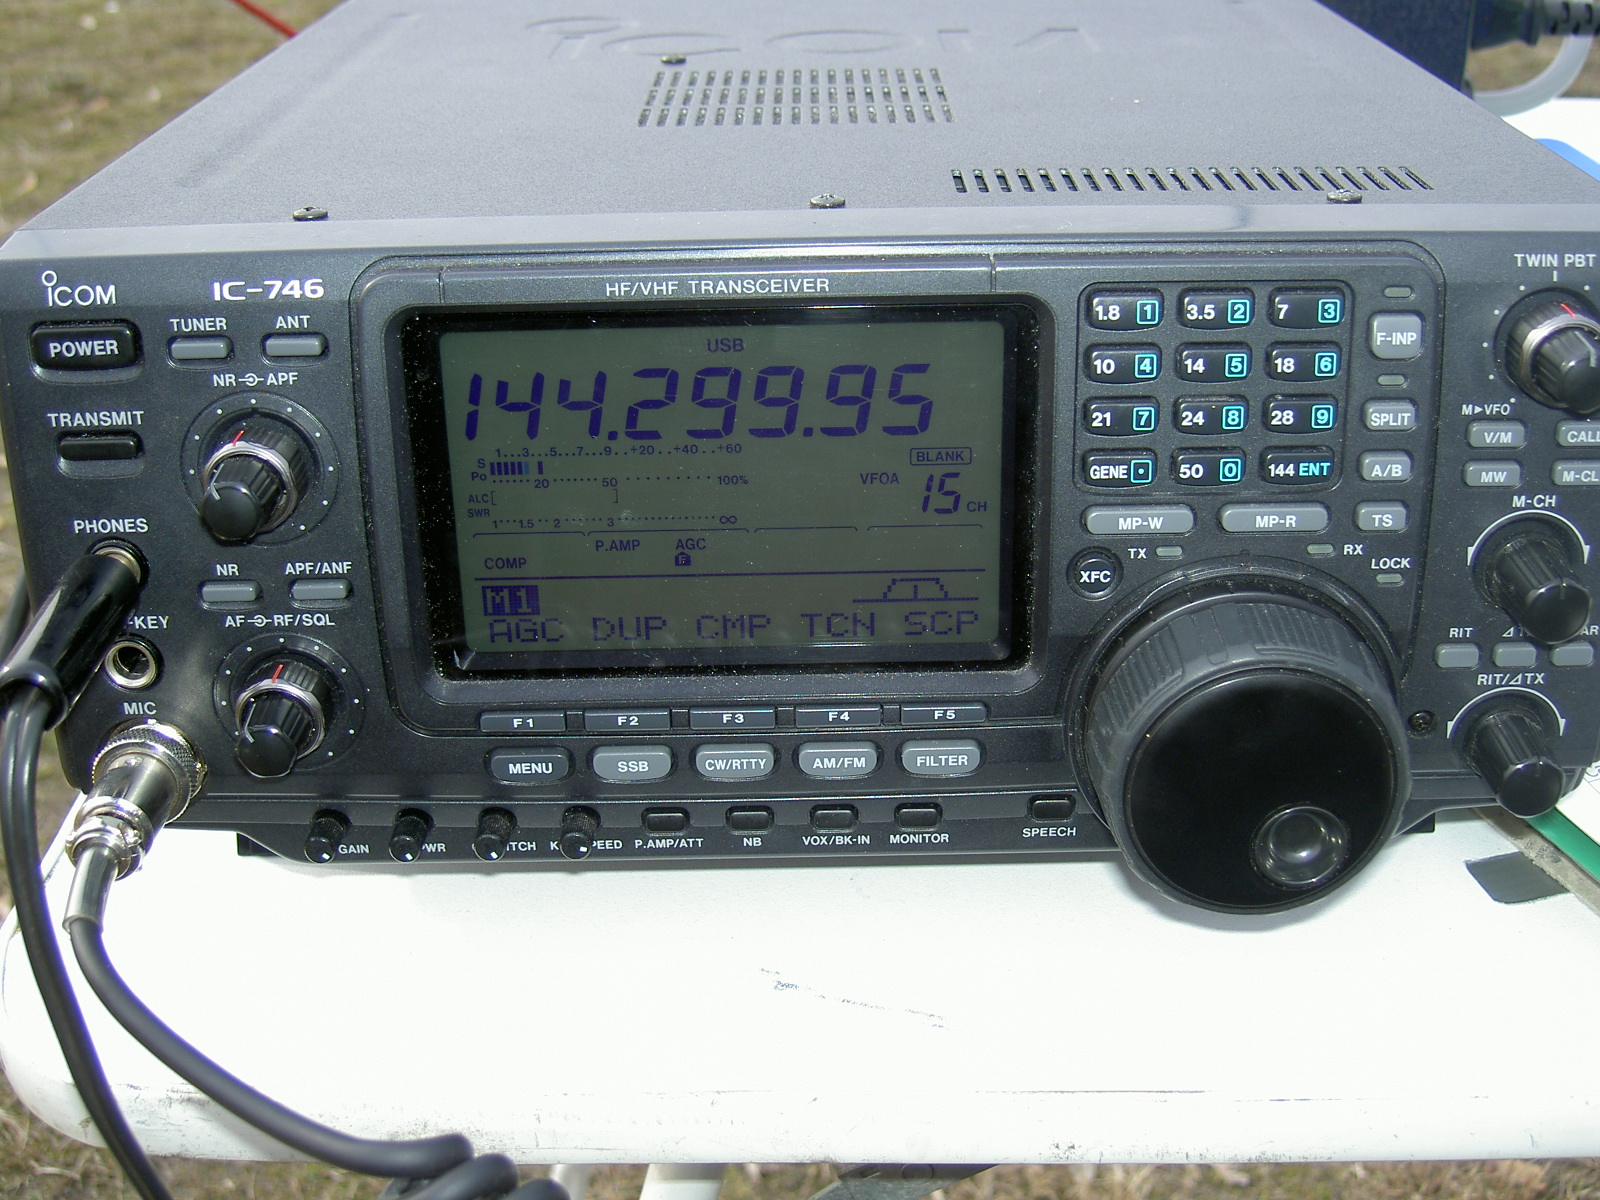
\includegraphics[width=0.85\textwidth]{foto/117}
    \caption{\scriptsize Ein Transceiver (Funkgerät) für den Amateurfunk}
    \label{n_erste_schritte_transceiver}
\end{figure}

    \end{column}
   \begin{column}{0.48\textwidth}
       \begin{itemize}
  \item Jeder darf Funkgeräte kaufen und besitzen
  \item und Amateurfunksendungen empfangen
  \end{itemize}

   \end{column}
\end{columns}

\end{frame}

\begin{frame}
\only<1>{
\begin{QQuestion}{VD102}{Was gilt in Bezug auf den Empfang von Amateurfunkaussendungen?}{Die Anerkennung als \glqq SWL\grqq{} ist erforderlich in Verbindung mit der Mitgliedschaft in einer Amateurfunkvereinigung.}
{Es dürfen nur TKG-zugelassene Empfangsgeräte verwendet werden.}
{Es bedarf der Zuteilung eines Hörerrufzeichens aus der \glqq DE-Reihe\grqq{}.}
{Es ist keine Zulassung zur Teilnahme am Amateurfunkdienst erforderlich.}
\end{QQuestion}

}
\only<2>{
\begin{QQuestion}{VD102}{Was gilt in Bezug auf den Empfang von Amateurfunkaussendungen?}{Die Anerkennung als \glqq SWL\grqq{} ist erforderlich in Verbindung mit der Mitgliedschaft in einer Amateurfunkvereinigung.}
{Es dürfen nur TKG-zugelassene Empfangsgeräte verwendet werden.}
{Es bedarf der Zuteilung eines Hörerrufzeichens aus der \glqq DE-Reihe\grqq{}.}
{\textbf{\textcolor{DARCgreen}{Es ist keine Zulassung zur Teilnahme am Amateurfunkdienst erforderlich.}}}
\end{QQuestion}

}
\end{frame}

\begin{frame}
\frametitle{Ein Funkamateur darf senden}
\begin{columns}
    \begin{column}{0.48\textwidth}
    
\begin{figure}
    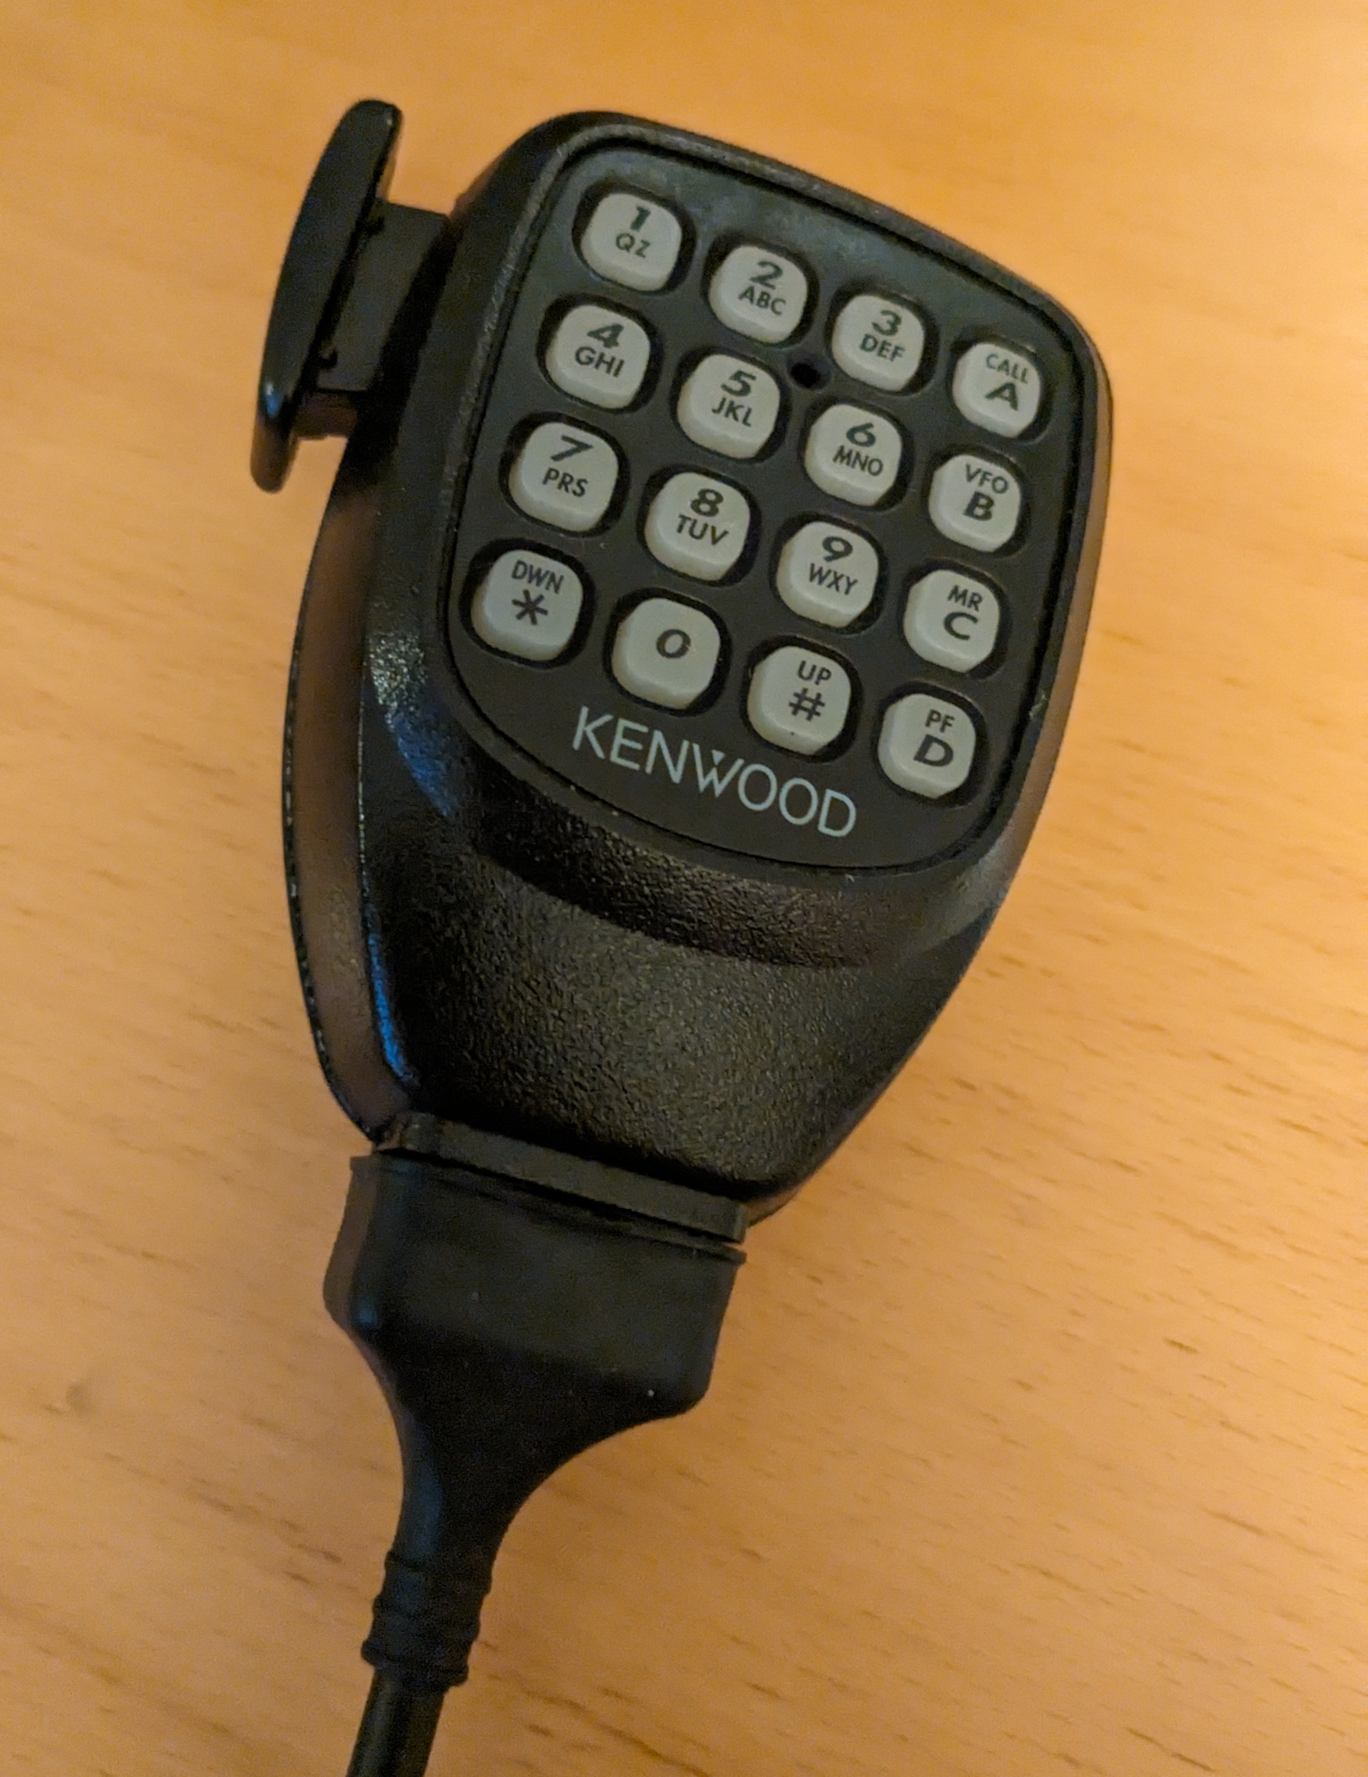
\includegraphics[width=0.85\textwidth]{foto/118}
    \caption{\scriptsize Handmikrofon mit PTT-Taste (links oben)}
    \label{n_erste_schritte_ptt}
\end{figure}

    \end{column}
   \begin{column}{0.48\textwidth}
       Auf Sendung gehen (die PTT-Taste drücken)

\begin{itemize}
  \item Taste am Funkgerät oder Mikrofon
  \item Schaltet den Transceiver von Empfangs- auf Sendebetrieb um
  \end{itemize}

   \end{column}
\end{columns}

\end{frame}

\begin{frame}
\only<1>{
\begin{QQuestion}{NF108}{Wie wird die Taste am Mikrofon bezeichnet, mit der man einen Transceiver auf Sendung schalten kann?}{RIT}
{VOX}
{PTT}
{SSB}
\end{QQuestion}

}
\only<2>{
\begin{QQuestion}{NF108}{Wie wird die Taste am Mikrofon bezeichnet, mit der man einen Transceiver auf Sendung schalten kann?}{RIT}
{VOX}
{\textbf{\textcolor{DARCgreen}{PTT}}}
{SSB}
\end{QQuestion}

}
\end{frame}

\begin{frame}
\frametitle{Mathematische Grundkenntnisse}
\begin{itemize}
  \item Im Amateurfunk werden Grundkenntnisse in Mathematik benötigt
  \item Je nach Klasse mehr Wissen notwendig
  \item Der Lehrgang unterstützt, kann aber nicht alles notwendige Wissen vermitteln
  \end{itemize}
\end{frame}

\begin{frame}
\only<1>{
\begin{QQuestion}{NA101}{Ein \qty{20}{\m} langer Draht wird bei 2/3 seiner Länge zertrennt. Wie lang sind die resultierenden Stücke in etwa?}{\qty{14,44}{\m} und \qty{5,56}{\m}}
{\qty{12,22}{\m} und \qty{7,78}{\m}}
{\qty{11,11}{\m} und \qty{8,89}{\m}}
{\qty{13,33}{\m} und \qty{6,67}{\m}}
\end{QQuestion}

}
\only<2>{
\begin{QQuestion}{NA101}{Ein \qty{20}{\m} langer Draht wird bei 2/3 seiner Länge zertrennt. Wie lang sind die resultierenden Stücke in etwa?}{\qty{14,44}{\m} und \qty{5,56}{\m}}
{\qty{12,22}{\m} und \qty{7,78}{\m}}
{\qty{11,11}{\m} und \qty{8,89}{\m}}
{\textbf{\textcolor{DARCgreen}{\qty{13,33}{\m} und \qty{6,67}{\m}}}}
\end{QQuestion}

}
\end{frame}

\begin{frame}
\only<1>{
\begin{QQuestion}{NA103}{Laut Datenblatt wiegen \qty{100}{\m} eines bestimmten Drahtes 210~g. Ein vorliegendes Drahtstück desselben Materials wiegt 55~g. Wie lang ist das Drahtstück in etwa?}{\qty{38,2}{\m}}
{\qty{382}{\m}}
{\qty{115}{\m}}
{\qty{26,2}{\m}}
\end{QQuestion}

}
\only<2>{
\begin{QQuestion}{NA103}{Laut Datenblatt wiegen \qty{100}{\m} eines bestimmten Drahtes 210~g. Ein vorliegendes Drahtstück desselben Materials wiegt 55~g. Wie lang ist das Drahtstück in etwa?}{\qty{38,2}{\m}}
{\qty{382}{\m}}
{\qty{115}{\m}}
{\textbf{\textcolor{DARCgreen}{\qty{26,2}{\m}}}}
\end{QQuestion}

}
\end{frame}

\begin{frame}
\only<1>{
\begin{QQuestion}{NA102}{Aus \qty{250}{\m} Draht sollen Antennen hergestellt werden. Pro Antenne werden \qty{18,5}{\m} benötigt. Wie viele Antennen können maximal aus dem vorhandenen Draht hergestellt werden?}{13}
{14}
{12}
{15}
\end{QQuestion}

}
\only<2>{
\begin{QQuestion}{NA102}{Aus \qty{250}{\m} Draht sollen Antennen hergestellt werden. Pro Antenne werden \qty{18,5}{\m} benötigt. Wie viele Antennen können maximal aus dem vorhandenen Draht hergestellt werden?}{\textbf{\textcolor{DARCgreen}{13}}}
{14}
{12}
{15}
\end{QQuestion}

}
\end{frame}%ENDCONTENT


\section{Rufzeichen}
\label{section:rufzeichen}
\begin{frame}%STARTCONTENT

\frametitle{Rufzeichen}
\begin{columns}
    \begin{column}{0.48\textwidth}
    
\begin{figure}
    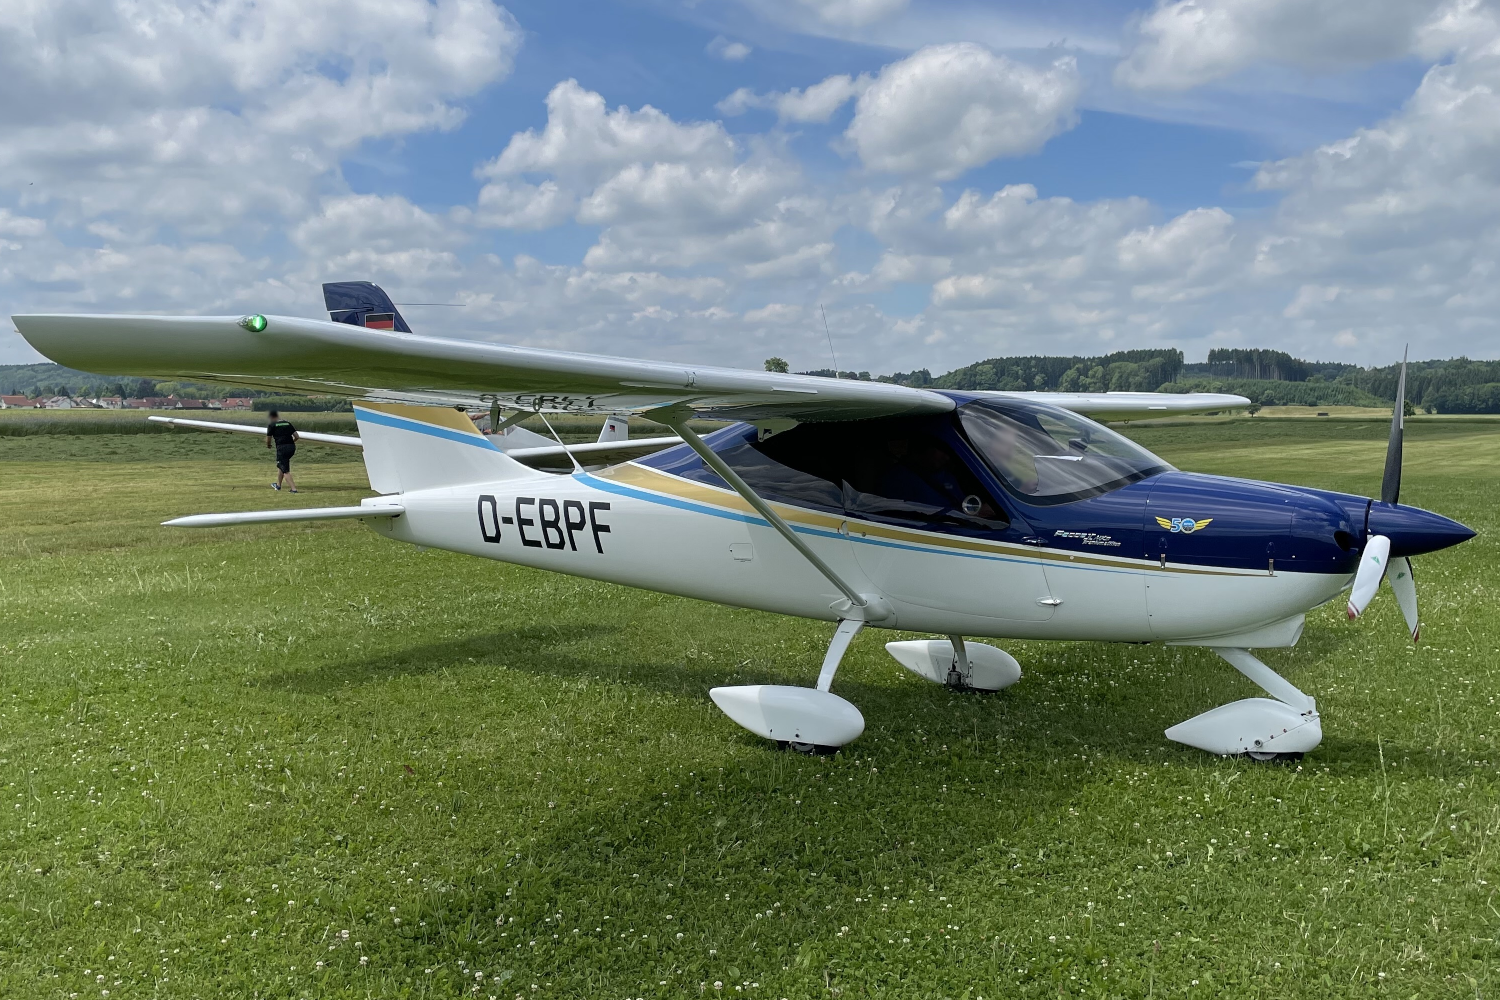
\includegraphics[width=0.85\textwidth]{foto/167}
    \caption{\scriptsize Flugzeug mit dem Rufzeichen DEBPF}
    \label{rufzeichen_flugzeug}
\end{figure}

    \end{column}
   \begin{column}{0.48\textwidth}
       \begin{itemize}
  \item Funkstationen verwenden Rufzeichen, um sich zu identifizieren
  \item Folge von Buchstaben und Ziffern
  \item Jedes mit Funk ausgerüstete Flugzeug und Schiff hat ein Rufzeichen
  \end{itemize}

   \end{column}
\end{columns}

\end{frame}

\begin{frame}
\frametitle{Amateurfunkrufzeichen}
\begin{itemize}
  \item Persönliches Rufzeichen wird zugeteilt
  \item Weltweit eindeutig
  \item Muss am Anfang und Ende jeder Verbindung genannt werden
  \item Und alle 10 Minuten bei längeren Verbindungen
  \end{itemize}
\end{frame}

\begin{frame}
\only<1>{
\begin{QQuestion}{VD207}{Woran erkennt man eine Amateurfunkstelle im Funkbetrieb?}{Am Amateurfunkrufzeichen}
{Am benutzten Frequenzbereich}
{An der verwendeten Sendeart}
{An der Modulation}
\end{QQuestion}

}
\only<2>{
\begin{QQuestion}{VD207}{Woran erkennt man eine Amateurfunkstelle im Funkbetrieb?}{\textbf{\textcolor{DARCgreen}{Am Amateurfunkrufzeichen}}}
{Am benutzten Frequenzbereich}
{An der verwendeten Sendeart}
{An der Modulation}
\end{QQuestion}

}
\end{frame}

\begin{frame}
\only<1>{
\begin{QQuestion}{VD205}{Wann muss der Funkamateur sein Rufzeichen nennen?}{Mindestens alle 15~Minuten während einer Funkverbindung}
{Auf Verlangen einer anderen am Funkverkehr beteiligten Funkstelle}
{Am Anfang und am Ende jeder Funkverbindung sowie mindestens alle 10~Minuten}
{Spätestens 5~Minuten nach einer ununterbrochenen Aussendung}
\end{QQuestion}

}
\only<2>{
\begin{QQuestion}{VD205}{Wann muss der Funkamateur sein Rufzeichen nennen?}{Mindestens alle 15~Minuten während einer Funkverbindung}
{Auf Verlangen einer anderen am Funkverkehr beteiligten Funkstelle}
{\textbf{\textcolor{DARCgreen}{Am Anfang und am Ende jeder Funkverbindung sowie mindestens alle 10~Minuten}}}
{Spätestens 5~Minuten nach einer ununterbrochenen Aussendung}
\end{QQuestion}

}
\end{frame}%ENDCONTENT


\section{Internationale Buchstabiertafel}
\label{section:buchstabiertafel}
\begin{frame}%STARTCONTENT
\begin{itemize}
  \item Manche Buchstaben lassen sich schwer voneinander unterscheiden
  \item Noch schwieriger bei leisem oder schlechtem Empfang
  \end{itemize}

\end{frame}

\begin{frame}
\frametitle{Lösung}
\begin{itemize}
  \item Jedem Buchstaben wird ein Wort zugeordnet
  \item Anstatt des Buchstabens wird das Wort ausgesprochen
  \end{itemize}
\end{frame}

\begin{frame}
\frametitle{Buchstabiertafeln}
\begin{itemize}
  \item In Deutschland ist die deutsche Buchstabiertafel bekannt
  \item Im Amateurfunk wird die internationale Buchstabiertafel verwendet
  \item Erste Einführung 1927 durch die International Telecommunication Union (ITU)
  \item Anhang 14 der Radio Regulations (RR)
  \item Wird auch in der Luftfahrt, dem Seefunk und von der NATO verwendet
  \end{itemize}

\end{frame}

\begin{frame}
\begin{columns}
    \begin{column}{0.48\textwidth}
    \begin{table}
\begin{DARCtabular}{cll}
     Buchstabe  & Wort  & Aussprache   \\
     A  & Alfa  & AL-FA   \\
     B  & Bravo  & BRA-WO   \\
     C  & Charlie  & TSCHA-LI   \\
     D  & Delta  & DELL-TA   \\
     E  & Echo  & ECK-KO   \\
     F  & Foxtrot  & FOX-TROTT   \\
     G  & Golf  & GOLF   \\
     H  & Hotel  & HO-TELL   \\
     I  & India  & IN-DI-AH   \\
     J  & Juliett  & DJU-LI-ETT   \\
     K  & Kilo  & KI-LO   \\
     L  & Lima  & LI-MA   \\
     M  & Mike  & MAIK   \\
\end{DARCtabular}
\caption{Die ITU-Buchstabiertafel}
\label{n_buchstabiertafel_1}
\end{table}

    \end{column}
   \begin{column}{0.48\textwidth}
       \begin{table}
\begin{DARCtabular}{cll}
     Buchstabe  & Wort  & Aussprache   \\
     N  & November  & NO-WEM-BER   \\
     O  & Oscar  & OSS-KAR   \\
     P  & Papa  & PA-PA   \\
     Q  & Quebec  & KWE-BECK   \\
     R  & Romeo  & RO-MI-O   \\
     S  & Sierra  & SIER-RA   \\
     T  & Tango  & TÄNG-GO   \\
     U  & Uniform  & JU-NI-FORM   \\
     V  & Victor  & WICK-TOR   \\
     W  & Whiskey  & WISS-KI   \\
     X  & X-ray  & ÄX-RÄI   \\
     Y  & Yankee  & JENG-KI   \\
     Z  & Zulu  & SUH-LUH   \\
\end{DARCtabular}
\caption{Die ITU-Buchstabiertafel}
\label{n_buchstabiertafel_2}
\end{table}

   \end{column}
\end{columns}

\end{frame}

\begin{frame}
\only<1>{
\begin{QQuestion}{VD206}{Welches Buchstabieralphabet ist nach der Verfügung 13/2005 bei der Nennung des Rufzeichens zur Identifikation einer Amateurfunkstation zu verwenden?}{Das englische Buchstabieralphabet der ITU-Konferenz in Madrid von 1932}
{Das europäische Buchstabieralphabet von 1992}
{Das internationale Buchstabieralphabet nach den Radio Regulations (Anhang 14)}
{Das deutsche Buchstabieralphabet nach DIN 5009}
\end{QQuestion}

}
\only<2>{
\begin{QQuestion}{VD206}{Welches Buchstabieralphabet ist nach der Verfügung 13/2005 bei der Nennung des Rufzeichens zur Identifikation einer Amateurfunkstation zu verwenden?}{Das englische Buchstabieralphabet der ITU-Konferenz in Madrid von 1932}
{Das europäische Buchstabieralphabet von 1992}
{\textbf{\textcolor{DARCgreen}{Das internationale Buchstabieralphabet nach den Radio Regulations (Anhang 14)}}}
{Das deutsche Buchstabieralphabet nach DIN 5009}
\end{QQuestion}

}
\end{frame}

\begin{frame}
\only<1>{
\begin{QQuestion}{BA103}{Wie wird das Rufzeichen \glqq DK5WP\grqq{} mit dem internationalen Buchstabieralphabet  buchstabiert?}{Delta Kilowatt 5 Whiskey Paris}
{Delta Kilo 5 William Paris}
{Delta Kilo 5 Whiskey Papa}
{Delta Kilowatt 5 William Papa}
\end{QQuestion}

}
\only<2>{
\begin{QQuestion}{BA103}{Wie wird das Rufzeichen \glqq DK5WP\grqq{} mit dem internationalen Buchstabieralphabet  buchstabiert?}{Delta Kilowatt 5 Whiskey Paris}
{Delta Kilo 5 William Paris}
{\textbf{\textcolor{DARCgreen}{Delta Kilo 5 Whiskey Papa}}}
{Delta Kilowatt 5 William Papa}
\end{QQuestion}

}
\end{frame}

\begin{frame}
\only<1>{
\begin{QQuestion}{BA104}{Wie wird das Rufzeichen \glqq DL1FLO\grqq{} mit dem internationalen Buchstabieralphabet  buchstabiert?}{Delta Lima 1 Florida Lima Oslo}
{Delta London 1 Foxtrot London Oslo}
{Delta Lima 1 Foxtrot Lima Oscar}
{Delta London 1 Florida London Oscar}
\end{QQuestion}

}
\only<2>{
\begin{QQuestion}{BA104}{Wie wird das Rufzeichen \glqq DL1FLO\grqq{} mit dem internationalen Buchstabieralphabet  buchstabiert?}{Delta Lima 1 Florida Lima Oslo}
{Delta London 1 Foxtrot London Oslo}
{\textbf{\textcolor{DARCgreen}{Delta Lima 1 Foxtrot Lima Oscar}}}
{Delta London 1 Florida London Oscar}
\end{QQuestion}

}
\end{frame}

\begin{frame}
\only<1>{
\begin{QQuestion}{BA110}{Wie wird das Rufzeichen \glqq IG9/DL4HR\grqq{} mit dem internationalen Buchstabieralphabet  buchstabiert?}{Italy Golf 9 Stroke Delta Lima 4 Honolulu Romeo}
{India Guatemala 9 Stroke Delta Lima 4 Honolulu Romeo}
{India Golf 9 Stroke Delta Lima 4 Hotel Romeo}
{Italy Guatemala 9 Stroke Delta Lima 4 Hotel Romeo}
\end{QQuestion}

}
\only<2>{
\begin{QQuestion}{BA110}{Wie wird das Rufzeichen \glqq IG9/DL4HR\grqq{} mit dem internationalen Buchstabieralphabet  buchstabiert?}{Italy Golf 9 Stroke Delta Lima 4 Honolulu Romeo}
{India Guatemala 9 Stroke Delta Lima 4 Honolulu Romeo}
{\textbf{\textcolor{DARCgreen}{India Golf 9 Stroke Delta Lima 4 Hotel Romeo}}}
{Italy Guatemala 9 Stroke Delta Lima 4 Hotel Romeo}
\end{QQuestion}

}
\end{frame}

\begin{frame}
\only<1>{
\begin{QQuestion}{BA109}{Wie wird das Rufzeichen \glqq DO9XJZ\grqq{} mit dem internationalen Buchstabieralphabet  buchstabiert?}{Delta Oscar 9 Xavier Juliett Zebra}
{Delta Oscar 9 X-ray Japan Zebra}
{Delta Oscar 9 X-ray Juliett Zulu}
{Delta Oscar 9 Xavier Japan Zulu}
\end{QQuestion}

}
\only<2>{
\begin{QQuestion}{BA109}{Wie wird das Rufzeichen \glqq DO9XJZ\grqq{} mit dem internationalen Buchstabieralphabet  buchstabiert?}{Delta Oscar 9 Xavier Juliett Zebra}
{Delta Oscar 9 X-ray Japan Zebra}
{\textbf{\textcolor{DARCgreen}{Delta Oscar 9 X-ray Juliett Zulu}}}
{Delta Oscar 9 Xavier Japan Zulu}
\end{QQuestion}

}
\end{frame}

\begin{frame}
\only<1>{
\begin{QQuestion}{BA101}{Wie wird das Rufzeichen \glqq DD4UQ\grqq{} mit dem internationalen Buchstabieralphabet  buchstabiert?}{Delta Delta 4 Uruguay Queen}
{Delta Delta 4 Uniform Quebec}
{Denmark Denmark 4 Uniform Queen}
{Denmark Denmark 4 Uruguay Quebec}
\end{QQuestion}

}
\only<2>{
\begin{QQuestion}{BA101}{Wie wird das Rufzeichen \glqq DD4UQ\grqq{} mit dem internationalen Buchstabieralphabet  buchstabiert?}{Delta Delta 4 Uruguay Queen}
{\textbf{\textcolor{DARCgreen}{Delta Delta 4 Uniform Quebec}}}
{Denmark Denmark 4 Uniform Queen}
{Denmark Denmark 4 Uruguay Quebec}
\end{QQuestion}

}
\end{frame}

\begin{frame}
\only<1>{
\begin{QQuestion}{BA105}{Wie wird das Rufzeichen \glqq DL4YBZ\grqq{} mit dem internationalen Buchstabieralphabet  buchstabiert?}{Delta Lima 4 Ypsilon Baker Zulu}
{Delta Lima 4 Yankee Baker Zebra}
{Delta Lima 4 Ypsilon Bravo Zebra}
{Delta Lima 4 Yankee Bravo Zulu}
\end{QQuestion}

}
\only<2>{
\begin{QQuestion}{BA105}{Wie wird das Rufzeichen \glqq DL4YBZ\grqq{} mit dem internationalen Buchstabieralphabet  buchstabiert?}{Delta Lima 4 Ypsilon Baker Zulu}
{Delta Lima 4 Yankee Baker Zebra}
{Delta Lima 4 Ypsilon Bravo Zebra}
{\textbf{\textcolor{DARCgreen}{Delta Lima 4 Yankee Bravo Zulu}}}
\end{QQuestion}

}
\end{frame}

\begin{frame}
\only<1>{
\begin{QQuestion}{BA106}{Wie wird das Rufzeichen \glqq DM4EAX\grqq{} mit dem internationalen Buchstabieralphabet  buchstabiert?}{Delta Madagascar 4 Echo Amerika X-ray}
{Delta Mike 4 Ecuador Amerika X-ray}
{Delta Mike 4 Echo Alfa X-ray}
{Delta Madagascar 4 Ecuador Alfa X-ray}
\end{QQuestion}

}
\only<2>{
\begin{QQuestion}{BA106}{Wie wird das Rufzeichen \glqq DM4EAX\grqq{} mit dem internationalen Buchstabieralphabet  buchstabiert?}{Delta Madagascar 4 Echo Amerika X-ray}
{Delta Mike 4 Ecuador Amerika X-ray}
{\textbf{\textcolor{DARCgreen}{Delta Mike 4 Echo Alfa X-ray}}}
{Delta Madagascar 4 Ecuador Alfa X-ray}
\end{QQuestion}

}
\end{frame}

\begin{frame}
\only<1>{
\begin{QQuestion}{BA102}{Wie wird das Rufzeichen \glqq DK1KC\grqq{} mit dem internationalen Buchstabieralphabet  buchstabiert?}{Delta Kilowatt 1 Kilowatt Caesar}
{Delta Kilo 1 Kilo Charlie}
{Denmark Kilo 1 Kilo Caesar}
{Denmark Kilowatt 1 Kilowatt Charlie}
\end{QQuestion}

}
\only<2>{
\begin{QQuestion}{BA102}{Wie wird das Rufzeichen \glqq DK1KC\grqq{} mit dem internationalen Buchstabieralphabet  buchstabiert?}{Delta Kilowatt 1 Kilowatt Caesar}
{\textbf{\textcolor{DARCgreen}{Delta Kilo 1 Kilo Charlie}}}
{Denmark Kilo 1 Kilo Caesar}
{Denmark Kilowatt 1 Kilowatt Charlie}
\end{QQuestion}

}
\end{frame}

\begin{frame}
\only<1>{
\begin{QQuestion}{BA107}{Wie wird das Rufzeichen \glqq DN9RO/p\grqq{} mit dem internationalen Buchstabieralphabet  buchstabiert?}{Delta November 9 Radio Oslo Stroke portable}
{Delta November 9 Romeo Oscar Stroke portable}
{Delta Nordpol 9 Radio Oslo Stroke portable}
{Delta Nordpol 9 Romeo Oscar Stroke portable}
\end{QQuestion}

}
\only<2>{
\begin{QQuestion}{BA107}{Wie wird das Rufzeichen \glqq DN9RO/p\grqq{} mit dem internationalen Buchstabieralphabet  buchstabiert?}{Delta November 9 Radio Oslo Stroke portable}
{\textbf{\textcolor{DARCgreen}{Delta November 9 Romeo Oscar Stroke portable}}}
{Delta Nordpol 9 Radio Oslo Stroke portable}
{Delta Nordpol 9 Romeo Oscar Stroke portable}
\end{QQuestion}

}
\end{frame}

\begin{frame}
\only<1>{
\begin{QQuestion}{BA108}{Wie wird das Rufzeichen \glqq DN9STV\grqq{} mit dem internationalen Buchstabieralphabet  buchstabiert?}{Delta November 9 Santiago Texas Victor}
{Delta November 9 Sierra Texas Vulcano}
{Delta November 9 Santiago Tango Vulcano}
{Delta November 9 Sierra Tango Victor}
\end{QQuestion}

}
\only<2>{
\begin{QQuestion}{BA108}{Wie wird das Rufzeichen \glqq DN9STV\grqq{} mit dem internationalen Buchstabieralphabet  buchstabiert?}{Delta November 9 Santiago Texas Victor}
{Delta November 9 Sierra Texas Vulcano}
{Delta November 9 Santiago Tango Vulcano}
{\textbf{\textcolor{DARCgreen}{Delta November 9 Sierra Tango Victor}}}
\end{QQuestion}

}
\end{frame}%ENDCONTENT


\section{Betriebsabwicklung}
\label{section:betriebsabwicklung}
\begin{frame}%STARTCONTENT

\frametitle{Ablauf im Amateurfunk}
\begin{itemize}
  \item Es gibt keine verpflichtenden Vorgaben außer Nennung des Rufzeichens
  \item Es macht aber Sinn, sich an der Betriebsabwicklung zu orientieren
  \end{itemize}

\end{frame}

\begin{frame}
\frametitle{Freie Frequenz finden}
\begin{itemize}
  \item Frequenzen werden gemeinsam genutzt
  \item Erst hören, ob die Frequenz frei ist
  \item Zwei- bis dreimal kurz nachfragen, ob die Frequenz frei ist
  \end{itemize}

\end{frame}

\begin{frame}
\frametitle{Anruf starten}
    \pause
    
\frametitle{Allgemeiner Anruf}
\begin{itemize}
  \item Geht an \emph{alle} Stationen
  \item Beginnt mit der internationalen Abkürzung \emph{CQ}
  \end{itemize}
    \pause
    
\frametitle{Gezielter Anruf}
\begin{itemize}
  \item Antwort von einer bestimmten Station erwartet
  \end{itemize}
    \pause
    In der Antwort wird erst das Rufzeichen der anrufenden Station, dann das eigene genannt

\end{frame}

\begin{frame}
\frametitle{Allgemeiner Anruf}
    \pause\QSOown{Ist diese Frequenz frei? DL1PZ}\pause\QSOother{\emph{(keine Antwort)}}\pause\QSOown{Ist diese Frequenz frei? DL1PZ}\pause\QSOother{\emph{(keine Antwort)}}\pause\QSOown{CQ CQ hier ist DL1PZ mit einem allgemeinen Anruf, hier ist DL1PZ und hört.}\pause\QSOother{DL1PZ hier ist DL9MJ bitte kommen}


\end{frame}

\begin{frame}
\frametitle{Gezielter Anruf}
    \pause\QSOown{DL9MJ für DL1PZ bitte kommen}\pause\QSOother{DL1PZ hier ist DL9MJ}


\end{frame}

\begin{frame}
\only<1>{
\begin{QQuestion}{BB102}{Was bedeutet die betriebliche Abkürzung \glqq CQ\grqq{} im Amateurfunk?}{Allgemeiner Anruf}
{Telegrafie}
{Große Entfernung}
{Contest Query}
\end{QQuestion}

}
\only<2>{
\begin{QQuestion}{BB102}{Was bedeutet die betriebliche Abkürzung \glqq CQ\grqq{} im Amateurfunk?}{\textbf{\textcolor{DARCgreen}{Allgemeiner Anruf}}}
{Telegrafie}
{Große Entfernung}
{Contest Query}
\end{QQuestion}

}
\end{frame}

\begin{frame}
\only<1>{
\begin{QQuestion}{BE105}{Sie möchten einen Allgemeinen Anruf in Telefonie im \qty{10}{\m}-Band beginnen. Sie finden eine Frequenz, auf der Sie keine Signale hören. Wie gehen Sie vor?}{Ich frage zwei- bis dreimal, ob die Frequenz besetzt ist. Erfolgt keine Antwort, rufe ich CQ.}
{Ich beobachte die Frequenz für einige Sekunden. Wenn ich weiterhin keine Signale höre, rufe ich CQ.}
{Da ich auf der Frequenz kein Signal höre, kann ich mit meinem CQ-Ruf beginnen.}
{Ich stimme meinen Sender auf der Frequenz ab und starte dann meinen CQ-Ruf.}
\end{QQuestion}

}
\only<2>{
\begin{QQuestion}{BE105}{Sie möchten einen Allgemeinen Anruf in Telefonie im \qty{10}{\m}-Band beginnen. Sie finden eine Frequenz, auf der Sie keine Signale hören. Wie gehen Sie vor?}{\textbf{\textcolor{DARCgreen}{Ich frage zwei- bis dreimal, ob die Frequenz besetzt ist. Erfolgt keine Antwort, rufe ich CQ.}}}
{Ich beobachte die Frequenz für einige Sekunden. Wenn ich weiterhin keine Signale höre, rufe ich CQ.}
{Da ich auf der Frequenz kein Signal höre, kann ich mit meinem CQ-Ruf beginnen.}
{Ich stimme meinen Sender auf der Frequenz ab und starte dann meinen CQ-Ruf.}
\end{QQuestion}

}
\end{frame}

\begin{frame}
\only<1>{
\begin{QQuestion}{BE101}{Wie können Sie eine Amateurfunkverbindung zum Beispiel beginnen?}{Durch Benutzen der internationalen Betriebsabkürzung CQ bzw. mit einem allgemeinen Anruf; mit einem gezielten Anruf an eine bestimmte Station oder mit einer Antwort auf einen allgemeinen Anruf, jeweils mit Nennung des eigenen Rufzeichens.}
{Durch wiederholtes Aussenden der internationalen Q-Gruppe \glqq QRZ?\grqq{} mit angehängtem eigenen Rufzeichen und dem Abhören der Frequenz in den Sendepausen.}
{Durch mehrmaliges, bei schlechten Ausbreitungsbedingungen häufiges Aussenden der Abkürzung CQ, des eigenen Rufzeichens und der Q-Gruppe \glqq QTH\grqq{} mit Zwischenhören.}
{Durch das Aussenden Ihres Rufzeichens und des in der IARU festgelegten Auftasttones von \qty{1750}{\Hz}, durch den die abhörenden Stationen Ihren Verbindungswunsch erkennen.}
\end{QQuestion}

}
\only<2>{
\begin{QQuestion}{BE101}{Wie können Sie eine Amateurfunkverbindung zum Beispiel beginnen?}{\textbf{\textcolor{DARCgreen}{Durch Benutzen der internationalen Betriebsabkürzung CQ bzw. mit einem allgemeinen Anruf; mit einem gezielten Anruf an eine bestimmte Station oder mit einer Antwort auf einen allgemeinen Anruf, jeweils mit Nennung des eigenen Rufzeichens.}}}
{Durch wiederholtes Aussenden der internationalen Q-Gruppe \glqq QRZ?\grqq{} mit angehängtem eigenen Rufzeichen und dem Abhören der Frequenz in den Sendepausen.}
{Durch mehrmaliges, bei schlechten Ausbreitungsbedingungen häufiges Aussenden der Abkürzung CQ, des eigenen Rufzeichens und der Q-Gruppe \glqq QTH\grqq{} mit Zwischenhören.}
{Durch das Aussenden Ihres Rufzeichens und des in der IARU festgelegten Auftasttones von \qty{1750}{\Hz}, durch den die abhörenden Stationen Ihren Verbindungswunsch erkennen.}
\end{QQuestion}

}
\end{frame}

\begin{frame}
\only<1>{
\begin{QQuestion}{BE102}{Wie sollten Sie antworten, wenn jemand in Telefonie CQ ruft?}{Ich rufe ebenfalls CQ und nenne das Rufzeichen der rufenden Station mindestens dreimal, anschließend sage ich mindestens fünfmal: \glqq Hier ist (eigenes Rufzeichen buchstabieren)\grqq{}.}
{Ich nenne das Rufzeichen der rufenden Station mindestens fünfmal, und anschließend sage ich mindestens einmal: \glqq Hier ist (eigenes Rufzeichen buchstabieren)\grqq{}.}
{Ich nenne das Rufzeichen der rufenden Station einmal, anschließend sage ich einmal: \glqq Hier ist (eigenes Rufzeichen buchstabieren), bitte kommen\grqq{}.}
{Ich nenne mein Rufzeichen und fordere die rufende Station auf, auf einer anderen Frequenz weiter zu rufen (mindestens zweimal).}
\end{QQuestion}

}
\only<2>{
\begin{QQuestion}{BE102}{Wie sollten Sie antworten, wenn jemand in Telefonie CQ ruft?}{Ich rufe ebenfalls CQ und nenne das Rufzeichen der rufenden Station mindestens dreimal, anschließend sage ich mindestens fünfmal: \glqq Hier ist (eigenes Rufzeichen buchstabieren)\grqq{}.}
{Ich nenne das Rufzeichen der rufenden Station mindestens fünfmal, und anschließend sage ich mindestens einmal: \glqq Hier ist (eigenes Rufzeichen buchstabieren)\grqq{}.}
{\textbf{\textcolor{DARCgreen}{Ich nenne das Rufzeichen der rufenden Station einmal, anschließend sage ich einmal: \glqq Hier ist (eigenes Rufzeichen buchstabieren), bitte kommen\grqq{}.}}}
{Ich nenne mein Rufzeichen und fordere die rufende Station auf, auf einer anderen Frequenz weiter zu rufen (mindestens zweimal).}
\end{QQuestion}

}
\end{frame}

\begin{frame}
\frametitle{Unklare Verständigung}
    \pause\QSOown{D\emph{(krschkrsch)}MJ für DK5WP, bitte kommen}\pause\QSOother{Hier ist DL9MJ, wurde ich gerufen?}
    \pause
    Nachfragen, ob man gemeint war



\end{frame}

\begin{frame}
\only<1>{
\begin{QQuestion}{BE103}{Ihr Rufzeichen ist DH7RW. Sie hören unvollständig \glqq ...~7 Romeo Whiskey\grqq{}. Wie reagieren Sie?}{Ich antworte: \glqq Bitte QSY!\grqq{}.}
{Ich antworte: \glqq Bitte QSL!\grqq{}    }
{Ich antworte: \glqq Hier ist DH7RW, wurde ich gerufen?\grqq{}}
{Ich freue mich auf eine Antwort aus 7R - Algerien.}
\end{QQuestion}

}
\only<2>{
\begin{QQuestion}{BE103}{Ihr Rufzeichen ist DH7RW. Sie hören unvollständig \glqq ...~7 Romeo Whiskey\grqq{}. Wie reagieren Sie?}{Ich antworte: \glqq Bitte QSY!\grqq{}.}
{Ich antworte: \glqq Bitte QSL!\grqq{}    }
{\textbf{\textcolor{DARCgreen}{Ich antworte: \glqq Hier ist DH7RW, wurde ich gerufen?\grqq{}}}}
{Ich freue mich auf eine Antwort aus 7R - Algerien.}
\end{QQuestion}

}
\end{frame}

\begin{frame}
\frametitle{Anruf beenden}
\begin{itemize}
  \item Die Frequenz wird der anrufenden Station überlassen
  \item Falls die antwortende Station zwischendurch von einer weiteren Station gerufen wurde, soll sie sich mit dieser auf eine andere Frequenz einigen, um der bisherigen Station die Frequenz zurückzugeben
  \end{itemize}
\end{frame}

\begin{frame}
\only<1>{
\begin{QQuestion}{BE108}{Sie haben eine Funkverbindung mit einer vorher \glqq CQ\grqq{} rufenden Station beendet. Anschließend werden Sie von einer anderen Station gerufen. Wie verhalten Sie sich?}{Ich bleibe auf der Frequenz und tätige ein QSO mit der neu rufenden Station.}
{Ich verständige mich mit der neuen Gegenstation auf eine andere Frequenz und führe dort das QSO weiter.}
{Ich gehe etwa \qty{1}{\kHz} neben die bisherige Frequenz und rufe dort die anrufende Station.}
{Ich reagiere nicht auf den Anruf, weil die Frequenz der Station gehört, die CQ gerufen hat.}
\end{QQuestion}

}
\only<2>{
\begin{QQuestion}{BE108}{Sie haben eine Funkverbindung mit einer vorher \glqq CQ\grqq{} rufenden Station beendet. Anschließend werden Sie von einer anderen Station gerufen. Wie verhalten Sie sich?}{Ich bleibe auf der Frequenz und tätige ein QSO mit der neu rufenden Station.}
{\textbf{\textcolor{DARCgreen}{Ich verständige mich mit der neuen Gegenstation auf eine andere Frequenz und führe dort das QSO weiter.}}}
{Ich gehe etwa \qty{1}{\kHz} neben die bisherige Frequenz und rufe dort die anrufende Station.}
{Ich reagiere nicht auf den Anruf, weil die Frequenz der Station gehört, die CQ gerufen hat.}
\end{QQuestion}

}
\end{frame}%ENDCONTENT


\section{Das RST-System}
\label{section:rst}
\begin{frame}%STARTCONTENT

\frametitle{Das RST-System}
Qualität der Funkverbindung hängt ab von

\begin{itemize}
  \item Sendeleistung
  \item verwendete Antenne
  \item Entfernung
  \item aktuelle Ausbreitungsbedingungen
  \end{itemize}
    \pause
    Im Rapport beschreibt die empfangende Station die Qualität der Verbindung

\end{frame}

\begin{frame}
\only<1>{
\begin{QQuestion}{BE201}{Was versteht man unter dem RST-Rapport? Es ist eine Kurzformel,~...}{um die Sendeleistung zu beschreiben.}
{um die Empfangsqualität zu beschreiben.}
{um den Ionosphärenzustand zu beschreiben.}
{um die Sonnenfleckenaktivität zu beschreiben.}
\end{QQuestion}

}
\only<2>{
\begin{QQuestion}{BE201}{Was versteht man unter dem RST-Rapport? Es ist eine Kurzformel,~...}{um die Sendeleistung zu beschreiben.}
{\textbf{\textcolor{DARCgreen}{um die Empfangsqualität zu beschreiben.}}}
{um den Ionosphärenzustand zu beschreiben.}
{um die Sonnenfleckenaktivität zu beschreiben.}
\end{QQuestion}

}
\end{frame}

\begin{frame}
\frametitle{RST-System}
\begin{table}
\begin{DARCtabular}{llll}
     Wert  & Bereich  & Bedeutung  & Englisch   \\
     R  & 1 -- 5  & Lesbarkeit  & Readability   \\
     S  & 1 -- 9  & Signalstärke  & Signal Strength   \\
     T  & 1 -- 9  & Tonqualität  & Tone   \\
\end{DARCtabular}
\caption{Die Bestandteile des RST-Rapports}
\label{n_rst}
\end{table}

\end{frame}

\begin{frame}
\frametitle{Readability}
Subjektive Bewertung des Lesbarkeit (Verständlichkeit)

\begin{table}
\begin{DARCtabular}{ll}
     R  & Beurteilung   \\
     1  & nicht lesbar   \\
     2  & zeitweise lesbar   \\
     3 & mit Schwierigkeiten lesbar   \\
     4  & ohne Schwierigkeiten lesbar   \\
     5  & einwandfrei lesbar   \\
\end{DARCtabular}
\caption{Anhaltspunkte für die subjektive Bewertung der Lesbarkeit (Verständlichkeit)}
\label{n_rst_r}
\end{table}
\end{frame}

\begin{frame}
\frametitle{Signal Strength}
Vom Funkgerät ablesen


\begin{figure}
    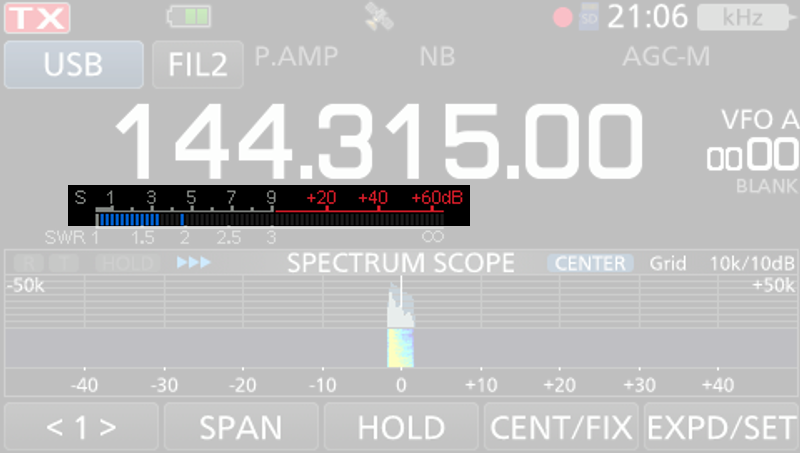
\includegraphics[width=0.85\textwidth]{foto/123}
    \caption{\scriptsize Display eines IC9700-Transceivers, hervorgehoben ist das S-Meter, das den aktuellen Empfangspegel anzeigt}
    \label{n_rst_s-meter}
\end{figure}

\end{frame}

\begin{frame}
\frametitle{Beispiele für RST-Rapporte}
im Sprechfunk

\begin{table}
\begin{DARCtabular}{llcl}
     Verständlichkeit  & S-Meter  &$\rightarrow$ & RST-Rapport   \\
     einwandfrei (=5)  & +\qty{20}{\dB}  &$\rightarrow$ & 59+20dB   \\
     einwandfrei (=5)  & 9  &$\rightarrow$ & 59   \\
     ohne Schwierigkeiten (=4)  & 5  &$\rightarrow$ & 45   \\
     mit Schwierigkeiten (=3)  & 3  &$\rightarrow$ & 33   \\
     unverständlich (=1)  & 3  &$\rightarrow$ & 13   \\
\end{DARCtabular}
\caption{Beispiele für RST-Rapporte im Sprechfunk}
\label{n_rst_beispiele}
\end{table}
\end{frame}

\begin{frame}
\only<1>{
\begin{QQuestion}{BE202}{Was bedeuten die Buchstaben RST, mit denen Sie die Empfangsqualität einer Sendung beurteilen können?}{R = Rufzeichen, S = Standort, T = Tonqualität}
{R = Rufzeichen, S = Signalstärke, T = Tonqualität}
{R = Lesbarkeit, S = Signalstärke, T = Trägerfrequenz}
{R = Lesbarkeit, S = Signalstärke, T = Tonqualität}
\end{QQuestion}

}
\only<2>{
\begin{QQuestion}{BE202}{Was bedeuten die Buchstaben RST, mit denen Sie die Empfangsqualität einer Sendung beurteilen können?}{R = Rufzeichen, S = Standort, T = Tonqualität}
{R = Rufzeichen, S = Signalstärke, T = Tonqualität}
{R = Lesbarkeit, S = Signalstärke, T = Trägerfrequenz}
{\textbf{\textcolor{DARCgreen}{R = Lesbarkeit, S = Signalstärke, T = Tonqualität}}}
\end{QQuestion}

}
\end{frame}

\begin{frame}
\only<1>{
\begin{QQuestion}{BE203}{In welcher Weise wird nach dem RST-System die Empfangsqualität einer Amateurfunkaussendung beurteilt?}{Lesbarkeit in Stufen von 1-5,  Signalstärke in Stufen von 1-5 und  Tonhöhe in Stufen von 1-9}
{Lesbarkeit in Stufen von 1-5,  Signalstärke in Stufen von 1-9 und  Tonqualität in Stufen von 1-9}
{Signalqualität in Stufen von 1-5,  Signalstärke in Stufen von 1-5 und  Tonqualität in Stufen von 1-9}
{Lesbarkeit in Stufen von 1-9,  Signalqualität in Stufen von 1-5 und  Tonhöhe in Stufen von 1-4}
\end{QQuestion}

}
\only<2>{
\begin{QQuestion}{BE203}{In welcher Weise wird nach dem RST-System die Empfangsqualität einer Amateurfunkaussendung beurteilt?}{Lesbarkeit in Stufen von 1-5,  Signalstärke in Stufen von 1-5 und  Tonhöhe in Stufen von 1-9}
{\textbf{\textcolor{DARCgreen}{Lesbarkeit in Stufen von 1-5,  Signalstärke in Stufen von 1-9 und  Tonqualität in Stufen von 1-9}}}
{Signalqualität in Stufen von 1-5,  Signalstärke in Stufen von 1-5 und  Tonqualität in Stufen von 1-9}
{Lesbarkeit in Stufen von 1-9,  Signalqualität in Stufen von 1-5 und  Tonhöhe in Stufen von 1-4}
\end{QQuestion}

}
\end{frame}

\begin{frame}
\only<1>{
\begin{PQuestion}{NF103}{Die Darstellung zeigt das Display eines Transceivers im Empfangsbetrieb. Wie wird die Anzeige 2 bezeichnet?}{Amplitudenspektrum}
{S-Meter}
{SWR-Meter}
{Wasserfalldiagramm}
{\DARCimage{1.0\linewidth}{579include}}\end{PQuestion}

}
\only<2>{
\begin{PQuestion}{NF103}{Die Darstellung zeigt das Display eines Transceivers im Empfangsbetrieb. Wie wird die Anzeige 2 bezeichnet?}{Amplitudenspektrum}
{\textbf{\textcolor{DARCgreen}{S-Meter}}}
{SWR-Meter}
{Wasserfalldiagramm}
{\DARCimage{1.0\linewidth}{579include}}\end{PQuestion}

}
\end{frame}

\begin{frame}
\only<1>{
\begin{QQuestion}{NF301}{Zu welchem Zweck dient das S-Meter in einem Transceiver?}{Es dient zur Anzeige der Sendeleistung.}
{Es dient zur Anzeige des Empfangspegels.}
{Es dient zur Anzeige der Empfängerverstärkung.}
{Es dient zur Anzeige der Audiolautstärke.}
\end{QQuestion}

}
\only<2>{
\begin{QQuestion}{NF301}{Zu welchem Zweck dient das S-Meter in einem Transceiver?}{Es dient zur Anzeige der Sendeleistung.}
{\textbf{\textcolor{DARCgreen}{Es dient zur Anzeige des Empfangspegels.}}}
{Es dient zur Anzeige der Empfängerverstärkung.}
{Es dient zur Anzeige der Audiolautstärke.}
\end{QQuestion}

}
\end{frame}

\begin{frame}Bei den folgenden Prüfungsfragen kommt es darauf an das S-Meter richtig abzulesen. In allen Prüfungsfragen wird von einem einwandfreien Signal in Telefonie (Sprechfunk) ausgegangen. Der R-Wert ist daher jeweils 5 und der T-Wert entfällt.

\end{frame}

\begin{frame}
\only<1>{
\begin{PQuestion}{BE204}{Sie hören die Gegenstation in SSB-Telefonie einwandfrei. Das Anzeigeinstrument Ihres Funkgerätes zeigt den dargestellten Zeigerausschlag. Welchen Rapport nach dem RST-System geben Sie?}{25}
{29}
{52}
{55}
{\DARCimage{1.0\linewidth}{421include}}\end{PQuestion}

}
\only<2>{
\begin{PQuestion}{BE204}{Sie hören die Gegenstation in SSB-Telefonie einwandfrei. Das Anzeigeinstrument Ihres Funkgerätes zeigt den dargestellten Zeigerausschlag. Welchen Rapport nach dem RST-System geben Sie?}{25}
{29}
{52}
{\textbf{\textcolor{DARCgreen}{55}}}
{\DARCimage{1.0\linewidth}{421include}}\end{PQuestion}

}
\end{frame}

\begin{frame}
\only<1>{
\begin{PQuestion}{BE205}{Sie hören die Gegenstation in SSB-Telefonie einwandfrei. Das Anzeigeinstrument Ihres Funkgerätes zeigt den dargestellten Zeigerausschlag. Welchen Rapport nach dem RST-System geben Sie?}{95}
{39}
{59}
{56}
{\DARCimage{1.0\linewidth}{420include}}\end{PQuestion}

}
\only<2>{
\begin{PQuestion}{BE205}{Sie hören die Gegenstation in SSB-Telefonie einwandfrei. Das Anzeigeinstrument Ihres Funkgerätes zeigt den dargestellten Zeigerausschlag. Welchen Rapport nach dem RST-System geben Sie?}{95}
{39}
{\textbf{\textcolor{DARCgreen}{59}}}
{56}
{\DARCimage{1.0\linewidth}{420include}}\end{PQuestion}

}
\end{frame}

\begin{frame}
\only<1>{
\begin{PQuestion}{BE206}{Sie hören die Gegenstation in SSB-Telefonie einwandfrei. Das Anzeigeinstrument Ihres Funkgerätes zeigt den dargestellten Zeigerausschlag. Welchen Rapport nach dem RST-System geben Sie?}{520}
{69}
{4,2}
{59+\qty{20}{\decibel}}
{\DARCimage{1.0\linewidth}{422include}}\end{PQuestion}

}
\only<2>{
\begin{PQuestion}{BE206}{Sie hören die Gegenstation in SSB-Telefonie einwandfrei. Das Anzeigeinstrument Ihres Funkgerätes zeigt den dargestellten Zeigerausschlag. Welchen Rapport nach dem RST-System geben Sie?}{520}
{69}
{4,2}
{\textbf{\textcolor{DARCgreen}{59+\qty{20}{\decibel}}}}
{\DARCimage{1.0\linewidth}{422include}}\end{PQuestion}

}
\end{frame}

\begin{frame}
\only<1>{
\begin{PQuestion}{BE207}{Sie hören in einem Funkgespräch in SSB-Telefonie die Gegenstation einwandfrei. Das Display Ihres Funkgerätes zeigt die abgebildeten Informationen an. Welchen Empfangsrapport nach dem RST-System geben Sie?}{100}
{7}
{55}
{1}
{\DARCimage{1.0\linewidth}{587include}}\end{PQuestion}

}
\only<2>{
\begin{PQuestion}{BE207}{Sie hören in einem Funkgespräch in SSB-Telefonie die Gegenstation einwandfrei. Das Display Ihres Funkgerätes zeigt die abgebildeten Informationen an. Welchen Empfangsrapport nach dem RST-System geben Sie?}{100}
{7}
{\textbf{\textcolor{DARCgreen}{55}}}
{1}
{\DARCimage{1.0\linewidth}{587include}}\end{PQuestion}

}
\end{frame}

\begin{frame}
\only<1>{
\begin{PQuestion}{BE208}{Sie hören in einem Funkgespräch in SSB-Telefonie die Gegenstation einwandfrei. Das Display Ihres Funkgerätes zeigt die abgebildeten Informationen an. Welchen Empfangsrapport nach dem RST-System geben Sie?}{80}
{12,5}
{59}
{95}
{\DARCimage{1.0\linewidth}{586include}}\end{PQuestion}

}
\only<2>{
\begin{PQuestion}{BE208}{Sie hören in einem Funkgespräch in SSB-Telefonie die Gegenstation einwandfrei. Das Display Ihres Funkgerätes zeigt die abgebildeten Informationen an. Welchen Empfangsrapport nach dem RST-System geben Sie?}{80}
{12,5}
{\textbf{\textcolor{DARCgreen}{59}}}
{95}
{\DARCimage{1.0\linewidth}{586include}}\end{PQuestion}

}
\end{frame}

\begin{frame}
\only<1>{
\begin{PQuestion}{BE209}{Sie hören in einem Funkgespräch in SSB-Telefonie die Gegenstation einwandfrei. Das Display Ihres Funkgerätes zeigt die abgebildeten Informationen an. Welchen Empfangsrapport nach dem RST-System geben Sie?}{59+\qty{20}{\decibel}}
{520}
{50}
{17}
{\DARCimage{1.0\linewidth}{588include}}\end{PQuestion}

}
\only<2>{
\begin{PQuestion}{BE209}{Sie hören in einem Funkgespräch in SSB-Telefonie die Gegenstation einwandfrei. Das Display Ihres Funkgerätes zeigt die abgebildeten Informationen an. Welchen Empfangsrapport nach dem RST-System geben Sie?}{\textbf{\textcolor{DARCgreen}{59+\qty{20}{\decibel}}}}
{520}
{50}
{17}
{\DARCimage{1.0\linewidth}{588include}}\end{PQuestion}

}
\end{frame}%ENDCONTENT


\section{Ausbildungsfunkbetrieb}
\label{section:ausbildungsfunk}
\begin{frame}%STARTCONTENT

\frametitle{Ausbildungsfunkbetrieb}
Es gibt zum Zweck der Ausbildung die Ausnahme, dass auch Nicht-Funkamateure auf Amateurfunkfrequenzen senden dürfen.

Unter unmittelbarer Anleitung und Aufsicht eines zugelassenen Funkamateurs der Klasse~E oder A.

\end{frame}

\begin{frame}
\only<1>{
\begin{QQuestion}{VD303}{Nicht-Funkamateure dürfen am Ausbildungsfunkbetrieb~...}{auch an Wochenenden ohne besondere Auflagen teilnehmen.}
{nur an Klubstationen unter Aufsicht eines Funkamateurs mit zugeteiltem Rufzeichen der Klasse A oder E teilnehmen.}
{nur unter unmittelbarer Anleitung und Aufsicht eines Funkamateurs mit zugeteiltem Rufzeichen der Klasse A oder E teilnehmen.}
{auch ohne Anleitung und Aufsicht des ausbildenden Funkamateurs teilnehmen.}
\end{QQuestion}

}
\only<2>{
\begin{QQuestion}{VD303}{Nicht-Funkamateure dürfen am Ausbildungsfunkbetrieb~...}{auch an Wochenenden ohne besondere Auflagen teilnehmen.}
{nur an Klubstationen unter Aufsicht eines Funkamateurs mit zugeteiltem Rufzeichen der Klasse A oder E teilnehmen.}
{\textbf{\textcolor{DARCgreen}{nur unter unmittelbarer Anleitung und Aufsicht eines Funkamateurs mit zugeteiltem Rufzeichen der Klasse A oder E teilnehmen.}}}
{auch ohne Anleitung und Aufsicht des ausbildenden Funkamateurs teilnehmen.}
\end{QQuestion}

}
\end{frame}

\begin{frame}
\frametitle{Abwicklung Ausbildungsfunkbetrieb}
\begin{itemize}
  \item Der Auszubildende benutzt das Rufzeichen des Ausbilders und hängt den Zusatz „/T“ an: DG2RON/T
  \item Ausgesprochen wird das als „Trainee”
  \end{itemize}

\end{frame}

\begin{frame}
\only<1>{
\begin{QQuestion}{VD306}{Von wem ist während des Ausbildungsfunkbetriebs der Rufzeichenzusatz \glqq /T\grqq{} bzw. \glqq /Trainee\grqq{} zu benutzen?}{Vom Verantwortlichen der Schulstation}
{Vom Ausbilder}
{Vom Auszubildenden und vom Ausbilder}
{Vom Auszubildenden}
\end{QQuestion}

}
\only<2>{
\begin{QQuestion}{VD306}{Von wem ist während des Ausbildungsfunkbetriebs der Rufzeichenzusatz \glqq /T\grqq{} bzw. \glqq /Trainee\grqq{} zu benutzen?}{Vom Verantwortlichen der Schulstation}
{Vom Ausbilder}
{Vom Auszubildenden und vom Ausbilder}
{\textbf{\textcolor{DARCgreen}{Vom Auszubildenden}}}
\end{QQuestion}

}
\end{frame}

\begin{frame}
\only<1>{
\begin{QQuestion}{BD209}{Der Funkamateur mit dem Rufzeichen DL1PZ möchte Ausbildungsfunkbetrieb im Sprechfunk durchführen. Welches Rufzeichen darf der Auszubildende verwenden?}{DL1PZ/Trainee}
{DL1PZ/Ausbildung}
{Ausbildung/DL1PZ}
{Trainee/DL1PZ}
\end{QQuestion}

}
\only<2>{
\begin{QQuestion}{BD209}{Der Funkamateur mit dem Rufzeichen DL1PZ möchte Ausbildungsfunkbetrieb im Sprechfunk durchführen. Welches Rufzeichen darf der Auszubildende verwenden?}{\textbf{\textcolor{DARCgreen}{DL1PZ/Trainee}}}
{DL1PZ/Ausbildung}
{Ausbildung/DL1PZ}
{Trainee/DL1PZ}
\end{QQuestion}

}
 \end{frame}%ENDCONTENT


\section{Offene Sprache}
\label{section:offene_sprache}
\begin{frame}%STARTCONTENT

\frametitle{Offene Sprache}
Im Amateurfunk darf nur offene Sprache verwendet werden.

\begin{itemize}
  \item Keine Verschleierungsverfahren wie geheime Codes
  \item Zulässig sind digitale Kodierungen, Morsezeichen und Abkürzungen
  \end{itemize}

\end{frame}

\begin{frame}
\only<1>{
\begin{QQuestion}{VD103}{Im Amateurfunkverkehr darf nur offene Sprache verwendet werden. Was gilt \underline{nicht} als offene Sprache und ist daher unzulässig?}{Digitale Übertragungsverfahren, die einen Decoder benötigen}
{Q-Gruppen und Amateurfunkabkürzungen}
{Sprachverschlüsselung zur Verschleierung des Inhalts}
{Morsetelegrafie und Fernschreiben}
\end{QQuestion}

}
\only<2>{
\begin{QQuestion}{VD103}{Im Amateurfunkverkehr darf nur offene Sprache verwendet werden. Was gilt \underline{nicht} als offene Sprache und ist daher unzulässig?}{Digitale Übertragungsverfahren, die einen Decoder benötigen}
{Q-Gruppen und Amateurfunkabkürzungen}
{\textbf{\textcolor{DARCgreen}{Sprachverschlüsselung zur Verschleierung des Inhalts}}}
{Morsetelegrafie und Fernschreiben}
\end{QQuestion}

}
\end{frame}%ENDCONTENT


\section{Funkverkehr nur mit Funkamateuren}
\label{section:nur_mit_afu_stellen}
\begin{frame}%STARTCONTENT

\frametitle{Funkverkehr nur mit Funkamateuren}
Eine Amateurfunkstation darf nur andere Amateurfunkstationen kontaktieren.

Es ist unzulässig, mit Funkstellen anderer Funkdienste zu funken.

\end{frame}

\begin{frame}
\only<1>{
\begin{QQuestion}{VC111}{Mit welchen Funkstellen darf der Funkamateur Funkverkehr abwickeln?}{Mit allen Funkstellen, die auf den Amateurfunkbändern tätig sind}
{Ausschließlich mit anderen Amateurfunkstellen}
{Mit anderen Amateurfunkstellen und Funkstellen der Behörden und Organisationen mit Sicherheitsaufgaben (BOS)}
{Mit anderen Amateurfunkstellen und Funkstellen des Flug- und/oder Seefunkdienstes}
\end{QQuestion}

}
\only<2>{
\begin{QQuestion}{VC111}{Mit welchen Funkstellen darf der Funkamateur Funkverkehr abwickeln?}{Mit allen Funkstellen, die auf den Amateurfunkbändern tätig sind}
{\textbf{\textcolor{DARCgreen}{Ausschließlich mit anderen Amateurfunkstellen}}}
{Mit anderen Amateurfunkstellen und Funkstellen der Behörden und Organisationen mit Sicherheitsaufgaben (BOS)}
{Mit anderen Amateurfunkstellen und Funkstellen des Flug- und/oder Seefunkdienstes}
\end{QQuestion}

}
\end{frame}

\begin{frame}
\only<1>{
\begin{QQuestion}{VD703}{Unter welchen Voraussetzungen darf ein Funkamateur mit seinem Amateurfunkgerät Funkverkehr im CB-Funk-Bereich durchführen?}{Der Funkamateur darf mit seiner Amateurfunkstelle unter keinen Umständen im CB-Funk-Bereich senden.}
{Wenn das Amateurfunkgerät vom Funkamateur so eingestellt wurde, dass die technischen Vorschriften für CB-Funkgeräte eingehalten werden}
{Wenn eine Genehmigung zum Betrieb von CB-Funkgeräten vorliegt}
{Wenn die Sendeleistung auf \qty{4}{\W} ERP bei FM und AM bzw. \qty{12}{\W} PEP bei SSB begrenzt wird}
\end{QQuestion}

}
\only<2>{
\begin{QQuestion}{VD703}{Unter welchen Voraussetzungen darf ein Funkamateur mit seinem Amateurfunkgerät Funkverkehr im CB-Funk-Bereich durchführen?}{\textbf{\textcolor{DARCgreen}{Der Funkamateur darf mit seiner Amateurfunkstelle unter keinen Umständen im CB-Funk-Bereich senden.}}}
{Wenn das Amateurfunkgerät vom Funkamateur so eingestellt wurde, dass die technischen Vorschriften für CB-Funkgeräte eingehalten werden}
{Wenn eine Genehmigung zum Betrieb von CB-Funkgeräten vorliegt}
{Wenn die Sendeleistung auf \qty{4}{\W} ERP bei FM und AM bzw. \qty{12}{\W} PEP bei SSB begrenzt wird}
\end{QQuestion}

}
\end{frame}

\begin{frame}
\frametitle{Nachrichtenübermittlung}
Darüber hinaus ist es auch grundsätzlich unzulässig, Nachrichten von oder an Nicht-Funkamateure zu übermitteln.

Die einzige Ausnahme sind Not- und Katastrophenfälle. Dann ist es erlaubt Nachrichten von und an Nicht-Funkamateure zu senden.

\end{frame}

\begin{frame}
\only<1>{
\begin{QQuestion}{VC112}{Darf ein Funkamateur Nachrichten, die nicht den Amateurfunkdienst betreffen, für und an Dritte übermitteln?}{Ja, jederzeit}
{Nein, unter keinen Umständen}
{Nur in Not- und Katastrophenfällen}
{Nur nach Aufforderung durch die zuständige Außenstelle der Bundesnetzagentur}
\end{QQuestion}

}
\only<2>{
\begin{QQuestion}{VC112}{Darf ein Funkamateur Nachrichten, die nicht den Amateurfunkdienst betreffen, für und an Dritte übermitteln?}{Ja, jederzeit}
{Nein, unter keinen Umständen}
{\textbf{\textcolor{DARCgreen}{Nur in Not- und Katastrophenfällen}}}
{Nur nach Aufforderung durch die zuständige Außenstelle der Bundesnetzagentur}
\end{QQuestion}

}
\end{frame}%ENDCONTENT


\section{Gewerbliche Nutzung}
\label{section:gewerblich}
\begin{frame}%STARTCONTENT

\frametitle{Gewerbliche Nutzung}
Der Amateurfunk darf nicht wirtschaftlich genutzt werden. Es ist also beispielsweise unzulässig, gegen Geld die Nutzung des Amateurfunks anzubieten oder den Amateurfunk für Absprachen in einem Unternehmen zu benutzen.

\end{frame}

\begin{frame}
\only<1>{
\begin{QQuestion}{VC114}{Darf die Amateurfunkstelle zu gewerblich-wirtschaftlichen Zwecken betrieben werden? Eine Amateurfunkstelle darf~...}{zum Zwecke des geschäftsmäßigen Erbringens von Telekommunikationsdiensten betrieben werden.}
{nach Anzeige des Gewerbes unter Angabe des Rufzeichens zu gewerblich-wirtschaftlichen Zwecken betrieben werden.}
{nicht zu gewerblich-wirtschaftlichen Zwecken betrieben werden.}
{nach Genehmigung durch die Bundesnetzagentur zu gewerblich-wirtschaftlichen Zwecken betrieben werden.}
\end{QQuestion}

}
\only<2>{
\begin{QQuestion}{VC114}{Darf die Amateurfunkstelle zu gewerblich-wirtschaftlichen Zwecken betrieben werden? Eine Amateurfunkstelle darf~...}{zum Zwecke des geschäftsmäßigen Erbringens von Telekommunikationsdiensten betrieben werden.}
{nach Anzeige des Gewerbes unter Angabe des Rufzeichens zu gewerblich-wirtschaftlichen Zwecken betrieben werden.}
{\textbf{\textcolor{DARCgreen}{nicht zu gewerblich-wirtschaftlichen Zwecken betrieben werden.}}}
{nach Genehmigung durch die Bundesnetzagentur zu gewerblich-wirtschaftlichen Zwecken betrieben werden.}
\end{QQuestion}

}
\end{frame}

\begin{frame}
\only<1>{
\begin{QQuestion}{VC115}{Zu welchem Zweck darf eine Amateurfunkstelle laut Amateurfunkgesetz (AFuG) \underline{nicht} betrieben werden?}{zur Kommunikation mit Weltraumfunkstellen}
{zur Erforschung der atmosphärischen Wellenausbreitung}
{zum geschäftsmäßigen Erbringen von Telekommunikationsdiensten}
{zu experimentellen Studien}
\end{QQuestion}

}
\only<2>{
\begin{QQuestion}{VC115}{Zu welchem Zweck darf eine Amateurfunkstelle laut Amateurfunkgesetz (AFuG) \underline{nicht} betrieben werden?}{zur Kommunikation mit Weltraumfunkstellen}
{zur Erforschung der atmosphärischen Wellenausbreitung}
{\textbf{\textcolor{DARCgreen}{zum geschäftsmäßigen Erbringen von Telekommunikationsdiensten}}}
{zu experimentellen Studien}
\end{QQuestion}

}
\end{frame}%ENDCONTENT


\title{DARC Amateurfunklehrgang Klasse NEA}
\author{Elektrische Schwingungen und Funkwellen}
\institute{Deutscher Amateur Radio Club e.\,V.}
\begin{frame}
\maketitle
\end{frame}

\section{Gleich- und  Wechselspannung}
\label{section:gleich_und_wechselspannung}
\begin{frame}%STARTCONTENT

\frametitle{Einführung in die elektrische Spannung}
\begin{columns}
    \begin{column}{0.48\textwidth}
    
\begin{figure}
    \DARCimage{0.85\linewidth}{713include}
    \caption{\scriptsize Positiv und negativ geladene Teilchen gleichverteilt in einem Gegenstand.}
    \label{n_frequenz_elektrische_ladungen}
\end{figure}


    \end{column}
   \begin{column}{0.48\textwidth}
       \begin{itemize}
  \item Alle Stoffe bestehen aus winzigen Teilchen, die elektrisch geladen sind
  \item Manche sind \enquote{positiv} (Plus) geladen
  \item Manche sind \enquote{negativ} (Minus) geladen
  \end{itemize}

   \end{column}
\end{columns}

\end{frame}

\begin{frame}
\begin{columns}
    \begin{column}{0.48\textwidth}
    
\begin{figure}
    \DARCimage{0.85\linewidth}{710include}
    \caption{\scriptsize Anziehung und Abstoßung von Ladungen}
    \label{n_ladungen}
\end{figure}


    \end{column}
   \begin{column}{0.48\textwidth}
       \begin{itemize}
  \item Gleich geladene Teilchen stoßen sich ab
  \item Unterschiedliche Ladungen ziehen sich an
  \item Die meisten Gegenstände sind elektrisch ausgeglichen
  \end{itemize}

   \end{column}
\end{columns}

\end{frame}

\begin{frame}
\frametitle{Ladungstrennung}
\begin{itemize}
  \item Ladungen lassen sich gezielt trennen
  \item In einer Batterie, Solarzelle oder einem Windkraftwerk
  \item Ladungen versuchen wieder zusammen zu kommen
  \item Es liegt eine elektrische \emph{Spannung} vor
  \item Geräte zur Trennung von Ladungen heißen \emph{Spannungsquelle}
  \end{itemize}
\end{frame}

\begin{frame}
\frametitle{Spannungsquelle}
\begin{itemize}
  \item Der positiv geladene Anschluss heißt Pluspol
  \item Der negativ geladene Anchluss heißt Minuspol
  \item Die Spannung kann unterschiedlich groß sein
  \item Spannungsquellen, bei denen die Pole ständig zwischen positiver und negativer Spannung schwingen, erzeugen Wechselspannung
  \end{itemize}
    \pause
    Die elektrische Spannung wird in der Einheit $\text{Volt}$ mit der Abkürzung $V$ gemessen.



\end{frame}

\begin{frame}
\frametitle{Elektrischer Verbraucher}
\begin{columns}
    \begin{column}{0.48\textwidth}
    
\begin{figure}
    \DARCimage{0.85\linewidth}{714include}
    \caption{\scriptsize Die Pole einer Batterie, am Minus-Pol befindet sich ein Überschuss an negativen Ladungen und am Plus-Pol ein Überschuss an positiven Ladungen, die Pole der Batterie sind verbunden, daher kann der Strom durch den Verbraucher fließen.}
    \label{n_frequenz_strom_fliesst}
\end{figure}


    \end{column}
   \begin{column}{0.48\textwidth}
       \begin{itemize}
  \item Wird ein elektrischer Verbraucher zwischen beiden Polen angeschlossen, bewegen sich die Ladungen
  \item Es fließt ein elektrischer Strom
  \item Die Ladungsbewegung endet bei einem Ausgleich der Ladungsträger an den Polen
  \end{itemize}

   \end{column}
\end{columns}

\end{frame}%ENDCONTENT


\section{Frequenz}
\label{section:frequenz}
\begin{frame}%STARTCONTENT

\frametitle{Wechselspannung}
\begin{itemize}
  \item Die Wechselspannung im Stromnetz schwingt 50 mal in der Sekunde
  \item Die Anzahl der Schwingungen pro Sekunde nennt man Frequenz
  \item Die Einheit ist Hertz mit der Abkürzung $\text{Hz}$
  \item \qty{1}{\hertz} $\rightarrow$ 1 Schwingung pro Sekunde
  \item Das Stromnetz hat eine Frequenz von $50\ \text{Hz}$
  \end{itemize}
\end{frame}

\begin{frame}
\frametitle{Einheit Hertz}
\begin{itemize}
  \item Misst die Frequenz
  \item $1\ \text{Hz}$ $\rightarrow$1 Schwingung pro Sekunde
  \item Benannt nach dem deutschen Physiker Heinrich Rudolf Hertz
  \item Erzeugte im Jahr 1886 als erster Mensch elektromagnetische Wellen und konnte sie nachweisen
  \end{itemize}
    \pause
    $$1 \ \text{Hz} = \dfrac{1}{\text{s}}$$



\end{frame}

\begin{frame}
\only<1>{
\begin{QQuestion}{NA206}{Welche Einheit wird üblicherweise für die Frequenz einer elektrischen Schwingung verwendet?}{Hertz (Hz)}
{Meter (m)}
{Meter pro Sekunde (m/s)}
{Sekunde pro Meter (s/m)}
\end{QQuestion}

}
\only<2>{
\begin{QQuestion}{NA206}{Welche Einheit wird üblicherweise für die Frequenz einer elektrischen Schwingung verwendet?}{\textbf{\textcolor{DARCgreen}{Hertz (Hz)}}}
{Meter (m)}
{Meter pro Sekunde (m/s)}
{Sekunde pro Meter (s/m)}
\end{QQuestion}

}
\end{frame}

\begin{frame}
\only<1>{
\begin{QQuestion}{NA207}{Wenn s für Sekunde steht, gilt für die Einheit der Frequenz~...}{Hz = $\dfrac{1}{\textrm{s}}$}
{Hz = s}
{Hz = s$^2$}
{Hz = $\dfrac{1}{\textrm{s}^2}$}
\end{QQuestion}

}
\only<2>{
\begin{QQuestion}{NA207}{Wenn s für Sekunde steht, gilt für die Einheit der Frequenz~...}{\textbf{\textcolor{DARCgreen}{Hz = $\dfrac{1}{\textrm{s}}$}}}
{Hz = s}
{Hz = s$^2$}
{Hz = $\dfrac{1}{\textrm{s}^2}$}
\end{QQuestion}

}
\end{frame}

\begin{frame}
\frametitle{Hohe Schwingungen}
\begin{itemize}
  \item Im Funk wird mit viel höheren Schwingungen gearbeitet
  \item z.B. 144.000.\qty{000}{\hertz}
  \item Abkürzung: \qty{144}{\mega\hertz} (Megahertz)
  \item Einheitenvorzeichen \enquote{M} vor \enquote{Hz} gesetzt
  \item Der Wert wird mit einer Million multipliziert
  \end{itemize}
\end{frame}

\begin{frame}\begin{table}
\begin{DARCtabular}{lrr}
     Bezeichnung  & Abkürzung  & Wert   \\
     1 Kilohertz  & \qty{1}{\kilo\hertz}  & \qty{1000}{\hertz}   \\
     1 Megahertz  & \qty{1}{\mega\hertz}  & \qty{1000000}{\hertz}   \\
     1 Gigahertz  & \qty{1}{\giga\hertz}  & \qty{1000000000}{\hertz}   \\
\end{DARCtabular}
\caption{Kurzschreibweise für große Frequenzen}
\label{n_frequenz_einheitenvorzeichen}
\end{table}
\end{frame}

\begin{frame}
\only<1>{
\begin{QQuestion}{NA212}{\qty{144000000}{\Hz} entspricht ...}{\qty{1,44}{\kHz}}
{\qty{144}{\kHz}}
{\qty{1,44}{\GHz}}
{\qty{144}{\MHz}}
\end{QQuestion}

}
\only<2>{
\begin{QQuestion}{NA212}{\qty{144000000}{\Hz} entspricht ...}{\qty{1,44}{\kHz}}
{\qty{144}{\kHz}}
{\qty{1,44}{\GHz}}
{\textbf{\textcolor{DARCgreen}{\qty{144}{\MHz}}}}
\end{QQuestion}

}
 \end{frame}

\begin{frame}
\frametitle{Frequenzen Klasse N}
In der Klasse~N dürfen drei Frequenzbereiche verwendet werden

\begin{itemize}
  \item \qty{28}{\mega\hertz} bis \qty{29,7}{\mega\hertz}
  \item \qty{144}{\mega\hertz} bis \qty{146}{\mega\hertz}
  \item \qty{430}{\mega\hertz} bis \qty{440}{\mega\hertz}
  \end{itemize}
    \pause
    In der Klasse~E und A kommen weitere Frequenzbereiche hinzu



\end{frame}

\begin{frame}
\only<1>{
\begin{QQuestion}{VD723}{In welchen Frequenzbereichen ist für Funkamateure mit Zulassung für die Klasse~N Sendebetrieb erlaubt?}{\qtyrange{28}{29.7}{\MHz}, \qtyrange{144}{146}{\MHz}, \qtyrange{430}{440}{\MHz}}
{\qtyrange{7}{7.2}{\MHz}, \qtyrange{14}{14.35}{\MHz}, \qtyrange{1240}{1300}{\MHz}}
{Auf allen dem Amateurfunk in Deutschland zugewiesenen Kurzwellen-Frequenzbereichen}
{Auf allen dem Amateurfunk in Deutschland zugewiesenen Frequenzbereichen oberhalb der Kurzwelle}
\end{QQuestion}

}
\only<2>{
\begin{QQuestion}{VD723}{In welchen Frequenzbereichen ist für Funkamateure mit Zulassung für die Klasse~N Sendebetrieb erlaubt?}{\textbf{\textcolor{DARCgreen}{\qtyrange{28}{29.7}{\MHz}, \qtyrange{144}{146}{\MHz}, \qtyrange{430}{440}{\MHz}}}}
{\qtyrange{7}{7.2}{\MHz}, \qtyrange{14}{14.35}{\MHz}, \qtyrange{1240}{1300}{\MHz}}
{Auf allen dem Amateurfunk in Deutschland zugewiesenen Kurzwellen-Frequenzbereichen}
{Auf allen dem Amateurfunk in Deutschland zugewiesenen Frequenzbereichen oberhalb der Kurzwelle}
\end{QQuestion}

}
 \end{frame}

\begin{frame}
\frametitle{Oszillator}
\begin{itemize}
  \item Ein Oszillator erzeugt elektrische Schwingungen in einem Funkgerät
  \item Beim Senden werden die Schwingungen auf die Antenne geleitet und als Funkwellen abgestrahlt
  \end{itemize}

\end{frame}

\begin{frame}
\only<1>{
\begin{QQuestion}{ND201}{Was verstehen Sie unter einem \glqq Oszillator\grqq ?}{Es ist ein Messgerät zur Anzeige von Schwingungen.}
{Es ist ein sehr schmales Filter.}
{Es ist ein Schwingungserzeuger.}
{Es ist ein Hochfrequenzverstärker.}
\end{QQuestion}

}
\only<2>{
\begin{QQuestion}{ND201}{Was verstehen Sie unter einem \glqq Oszillator\grqq ?}{Es ist ein Messgerät zur Anzeige von Schwingungen.}
{Es ist ein sehr schmales Filter.}
{\textbf{\textcolor{DARCgreen}{Es ist ein Schwingungserzeuger.}}}
{Es ist ein Hochfrequenzverstärker.}
\end{QQuestion}

}
\end{frame}

\begin{frame}
\frametitle{Frequenzmessung}
\begin{columns}
    \begin{column}{0.48\textwidth}
    
\begin{figure}
    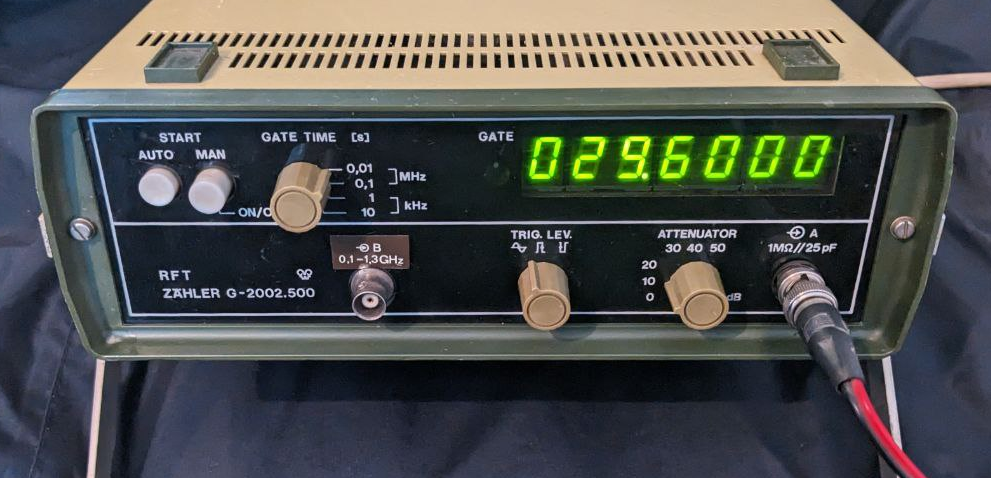
\includegraphics[width=0.85\textwidth]{foto/150}
    \caption{\scriptsize Frequenzzähler, der \qty{29,6}{\mega\hertz} misst}
    \label{frequenz_frequenzzaehler}
\end{figure}

    \end{column}
   \begin{column}{0.48\textwidth}
       \begin{itemize}
  \item Die genaue Sendefrequenz muss bekannt sein
  \item Die Messung erfolgt mit einem Frequenzzähler
  \item Zum Abgleich der Anzeige am Funkgerät
  \end{itemize}

   \end{column}
\end{columns}

\end{frame}

\begin{frame}
\only<1>{
\begin{QQuestion}{NI301}{Mit welchem Gerät kann die Sendefrequenz eines Senders gemessen werden?  }{Frequenzzähler}
{SWR-Meter}
{HF-Voltmeter}
{S-Meter}
\end{QQuestion}

}
\only<2>{
\begin{QQuestion}{NI301}{Mit welchem Gerät kann die Sendefrequenz eines Senders gemessen werden?  }{\textbf{\textcolor{DARCgreen}{Frequenzzähler}}}
{SWR-Meter}
{HF-Voltmeter}
{S-Meter}
\end{QQuestion}

}
\end{frame}%ENDCONTENT


\section{Sinusschwingung}
\label{section:sinusschwingung}
\begin{frame}%STARTCONTENT

\begin{columns}
    \begin{column}{0.48\textwidth}
    
\begin{figure}
    \DARCimage{0.85\linewidth}{725include}
    \caption{\scriptsize Die Spannung des Stromnetzes im zeitlichen Verlauf. Da die Spannung nicht die ganze Zeit den Höchstwert von \qty{325}{\volt} aufweist, wirkt sie effektiv übrigens nur mit \qty{230}{\volt}.}
    \label{n_frequenz_sinusschwingung}
\end{figure}


    \end{column}
   \begin{column}{0.48\textwidth}
       \begin{itemize}
  \item Die Wechselspannung aus dem Stromnetz schwingt nicht direkt zurück
  \item Es gibt einen sanften Übergang über 0
  \item Wie bei einem Pendel
  \item Diese Art der Schwingung ist eine Sinusschwingung
  \end{itemize}

   \end{column}
\end{columns}

\end{frame}

\begin{frame}
\begin{figure}
    \DARCimage{0.85\linewidth}{505include}
    \caption{\scriptsize Rechteckförmige Schwingung}
    \label{sinusschwingung_rechteck}
\end{figure}

\end{frame}

\begin{frame}
\begin{figure}
    \DARCimage{0.85\linewidth}{504include}
    \caption{\scriptsize Dreieckförmige Schwingung}
    \label{sinusschwingung_dreieck}
\end{figure}

\end{frame}

\begin{frame}
\begin{figure}
    \DARCimage{0.85\linewidth}{506include}
    \caption{\scriptsize Sägezahnförmige Schwingung}
    \label{sinusschwingung_saegezahn}
\end{figure}

\end{frame}

\begin{frame}
\only<1>{
\begin{question2x2}{NB401}{Welches Bild zeigt eine sinusförmige Wechselspannung?}{\DARCimage{1.0\linewidth}{505include}}
{\DARCimage{1.0\linewidth}{504include}}
{\DARCimage{1.0\linewidth}{503include}}
{\DARCimage{1.0\linewidth}{506include}}
\end{question2x2}

}
\only<2>{
\begin{question2x2}{NB401}{Welches Bild zeigt eine sinusförmige Wechselspannung?}{\DARCimage{1.0\linewidth}{505include}}
{\DARCimage{1.0\linewidth}{504include}}
{\textbf{\textcolor{DARCgreen}{\DARCimage{1.0\linewidth}{503include}}}}
{\DARCimage{1.0\linewidth}{506include}}
\end{question2x2}

}
\end{frame}%ENDCONTENT


\section{Amplitude und Periode}
\label{section:amplitude_periode}
\begin{frame}%STARTCONTENT

\frametitle{Amplitude}
\begin{columns}
    \begin{column}{0.48\textwidth}
    
\begin{figure}
    \DARCimage{0.85\linewidth}{726include}
    \caption{\scriptsize  Amplitude einer Sinusschwingung}
    \label{amplitude_periode_amplitudee}
\end{figure}


    \end{column}
   \begin{column}{0.48\textwidth}
       Der maximale Abstand von der Nulllinie zum höchsten oder tiefsten Punkt heißt \emph{Amplitude}


   \end{column}
\end{columns}

\end{frame}

\begin{frame}
\only<1>{
\begin{PQuestion}{NB404}{Was ist im Oszillogramm mit 1 markiert?}{Periode}
{Frequenz}
{Amplitude}
{Wellenlänge}
{\DARCimage{1.0\linewidth}{627include}}\end{PQuestion}

}
\only<2>{
\begin{PQuestion}{NB404}{Was ist im Oszillogramm mit 1 markiert?}{Periode}
{Frequenz}
{\textbf{\textcolor{DARCgreen}{Amplitude}}}
{Wellenlänge}
{\DARCimage{1.0\linewidth}{627include}}\end{PQuestion}

}
\end{frame}

\begin{frame}
\frametitle{Halbwellen}
\begin{columns}
    \begin{column}{0.48\textwidth}
    
\begin{figure}
    \DARCimage{0.85\linewidth}{727include}
    \caption{\scriptsize Positive und negative Halbwellen einer Sinusschwingung}
    \label{amplitude_periode_halbwellen}
\end{figure}


    \end{column}
   \begin{column}{0.48\textwidth}
       Bei einer Sinusschwingung gibt es positive und negative \emph{Halbwellen}


   \end{column}
\end{columns}

\end{frame}

\begin{frame}
\frametitle{Periode}
\begin{columns}
    \begin{column}{0.48\textwidth}
    
\begin{figure}
    \DARCimage{0.85\linewidth}{728include}
    \caption{\scriptsize Perioden einer Sinusschwingung}
    \label{amplitude_periode_perioden}
\end{figure}


    \end{column}
   \begin{column}{0.48\textwidth}
       Die Zeit ($t$) vom Beginn einer positiven Halbwelle bis zum Ende der darauf folgenden negativen Halbwelle heißt \emph{Periode} oder \emph{Periodendauer}


   \end{column}
\end{columns}

\end{frame}

\begin{frame}
\frametitle{Interaktiv}

\end{frame}

\begin{frame}
\only<1>{
\begin{PQuestion}{NB405}{Was ist im Oszillogramm mit 2 markiert?}{Spannung}
{Amplitude}
{Strom}
{Periode}
{\DARCimage{1.0\linewidth}{627include}}\end{PQuestion}

}
\only<2>{
\begin{PQuestion}{NB405}{Was ist im Oszillogramm mit 2 markiert?}{Spannung}
{Amplitude}
{Strom}
{\textbf{\textcolor{DARCgreen}{Periode}}}
{\DARCimage{1.0\linewidth}{627include}}\end{PQuestion}

}
 \end{frame}

\begin{frame}
\only<1>{
\begin{QQuestion}{NA213}{Welche Aussage ist für eine Schwingung von \num{145000000} Perioden pro Sekunde richtig?}{Ihre Ausbreitungsgeschwindigkeit beträgt \qty{145}{\km}/s.}
{Ihre Periodendauer beträgt \qty{145}{\us}.}
{Ihre Amplitude beträgt \qty{145}{\pps}.}
{Ihre Frequenz beträgt \qty{145}{\MHz}.}
\end{QQuestion}

}
\only<2>{
\begin{QQuestion}{NA213}{Welche Aussage ist für eine Schwingung von \num{145000000} Perioden pro Sekunde richtig?}{Ihre Ausbreitungsgeschwindigkeit beträgt \qty{145}{\km}/s.}
{Ihre Periodendauer beträgt \qty{145}{\us}.}
{Ihre Amplitude beträgt \qty{145}{\pps}.}
{\textbf{\textcolor{DARCgreen}{Ihre Frequenz beträgt \qty{145}{\MHz}.}}}
\end{QQuestion}

}

\end{frame}%ENDCONTENT


\section{Zehnerpotenzen}
\label{section:zehnerpotenzen}
\begin{frame}%STARTCONTENT

\frametitle{Große und kleine Werte}
\begin{itemize}
  \item Im Amateurfunk haben wir große und kleine Werte
  \item Um sich viele 0-en zu sparen, wurde bereits mit Einheitenvorsätzen abgekürzt, z.B. mit Milli (m) oder Kilo (k)
  \end{itemize}
\end{frame}

\begin{frame}
\frametitle{Zehnerpotenzen}
\begin{itemize}
  \item Einheitenvorsätze lassen sich in den meisten Taschenrechnern nicht direkt eingeben
  \item Stattdessen wird die Zehnerpotenz verwendet
  \item Kilo entspricht 1000 oder 10 $\cdot$ 10 $\cdot$ 10
  \item Abgekürzt 10<sup>3</sup>
  \end{itemize}
    \pause
    \qty{1500}{\hertz} $\rightarrow$ 1,5 kHz $\rightarrow$ 1,5 $\cdot$ 10<sup>3</sup> Hz

\qty{1500000}{\hertz} $\rightarrow$ \qty{1,5}{\mega\hertz} $\rightarrow$ 1,5 $\cdot$ 10<sup>6</sup> Hz

\end{frame}

\begin{frame}\begin{itemize}
  \item Milli entspricht  $\frac{1}{1000}$ oder $\frac{1}{10 \cdot 10 \cdot 10}$
  \item Abgekürzt 10<sup>-3</sup>
  \end{itemize}
    \pause
    \qty{0,0035}{\volt} $\rightarrow$ \qty{3,5}{\milli\volt} $\rightarrow$ 3,5 $\cdot$ 10<sup>-3</sup> V



\end{frame}

\begin{frame}
\frametitle{Einheitenvorsätze und Zehnerpotenzen}
\begin{table}
\begin{DARCtabular}{ccl}
     Bezeichnung  & Abkürzung  & Wert   \\
     Pico  & p  & 10<sup>-12</sup> = 0,000000000001   \\
     Nano  & n  & 10<sup>-9</sup> = 0,000000001   \\
     Mikro  & µ  & 10<sup>-6</sup> = 0,000001   \\
     Milli  & m  & 10<sup>-3</sup> = 0,001   \\
      &   & 10<sup>0</sup> = 1   \\
     Kilo  & k  & 10<sup>3</sup> = 1000   \\
     Mega  & M  & 10<sup>6</sup> = 1000000   \\
     Giga  & G  & 10<sup>9</sup> = 1000000000   \\
\end{DARCtabular}
\caption{Einheitenvorsätze für Zehnerpotenzen}
\label{e_einheitenvorzeichen}
\end{table}
\end{frame}

\begin{frame}
\frametitle{Taschenrechner}
\begin{columns}
    \begin{column}{0.48\textwidth}
    \begin{itemize}
  \item Taste \emph{EXP} oder \emph{$\cdot$10<sup>x</sup>}
  \item Eintippen: \enquote{145,3 Exp 6}
  \item Taste \emph{ENG} verschiebt den Exponent um 3
  \end{itemize}

    \end{column}
   \begin{column}{0.48\textwidth}
       
\begin{figure}
    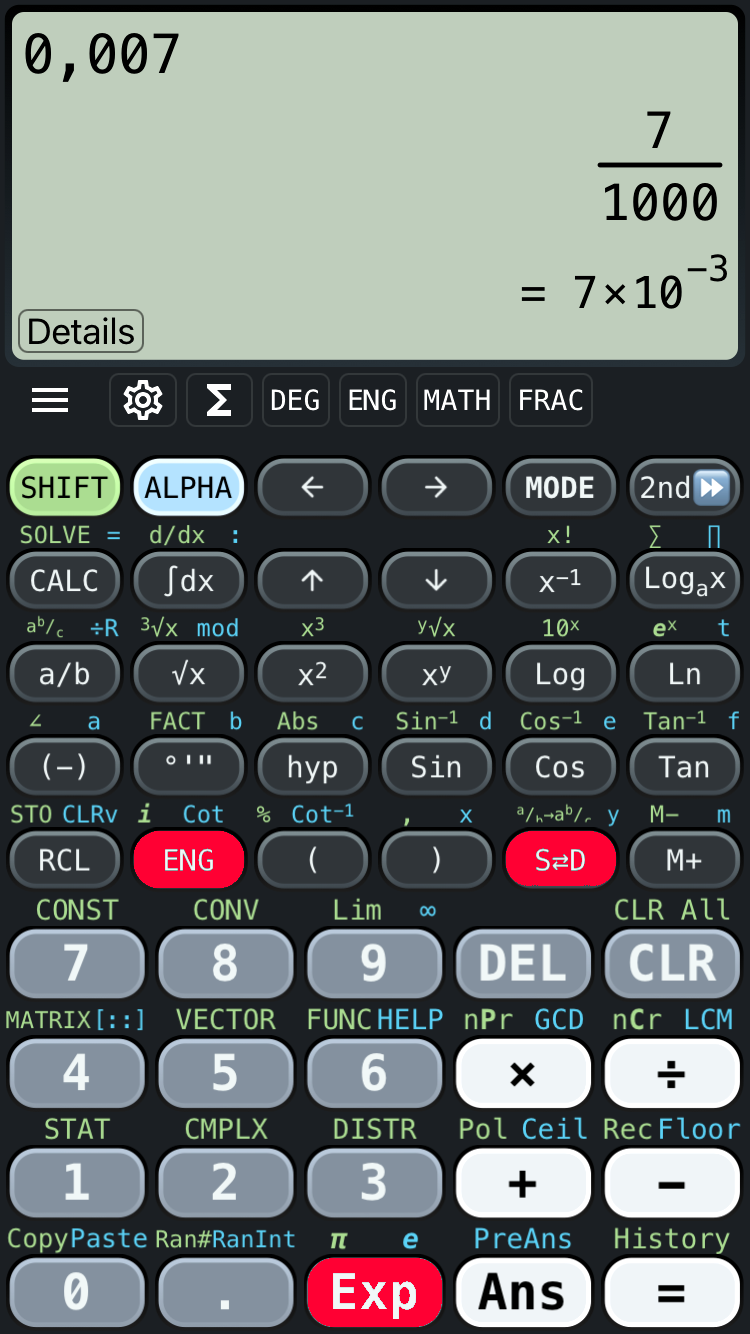
\includegraphics[width=0.85\textwidth]{foto/172}
    \caption{\scriptsize Verschiedene Darstellungen der Zahl 0,007 in einer Taschenrechner-App}
    \label{e_taschenrechner}
\end{figure}

   \end{column}
\end{columns}

\end{frame}

\begin{frame}
\only<1>{
\begin{QQuestion}{EA108}{\qty{0,00042}{\A} entspricht~...}{$420\cdot 10^6$ A.}
{$420\cdot 10^{-6}$ A.}
{$420\cdot 10^{-5}$ A.}
{$42\cdot 10^{-6}$ A.}
\end{QQuestion}

}
\only<2>{
\begin{QQuestion}{EA108}{\qty{0,00042}{\A} entspricht~...}{$420\cdot 10^6$ A.}
{\textbf{\textcolor{DARCgreen}{$420\cdot 10^{-6}$ A.}}}
{$420\cdot 10^{-5}$ A.}
{$42\cdot 10^{-6}$ A.}
\end{QQuestion}

}
\end{frame}

\begin{frame}
\only<1>{
\begin{QQuestion}{EA109}{\qty{0,042}{\A} entspricht~...}{$42\cdot 10^{-1}$ A.}
{$42\cdot 10^3$ A.}
{$42\cdot 10^{-2}$ A.}
{$42\cdot 10^{-3}$ A.}
\end{QQuestion}

}
\only<2>{
\begin{QQuestion}{EA109}{\qty{0,042}{\A} entspricht~...}{$42\cdot 10^{-1}$ A.}
{$42\cdot 10^3$ A.}
{$42\cdot 10^{-2}$ A.}
{\textbf{\textcolor{DARCgreen}{$42\cdot 10^{-3}$ A.}}}
\end{QQuestion}

}
\end{frame}

\begin{frame}
\only<1>{
\begin{QQuestion}{EA110}{\qty{4200000}{\Hz} entspricht~...}{$4,2\cdot 10^5$ Hz.}
{$4,2\cdot 10^6$ Hz.}
{$42\cdot 10^6$ Hz.}
{$42\cdot 10^{-5}$ Hz.}
\end{QQuestion}

}
\only<2>{
\begin{QQuestion}{EA110}{\qty{4200000}{\Hz} entspricht~...}{$4,2\cdot 10^5$ Hz.}
{\textbf{\textcolor{DARCgreen}{$4,2\cdot 10^6$ Hz.}}}
{$42\cdot 10^6$ Hz.}
{$42\cdot 10^{-5}$ Hz.}
\end{QQuestion}

}
\end{frame}

\begin{frame}
\only<1>{
\begin{QQuestion}{EA111}{\qty{0,01}{\mV} entspricht~...}{$1\cdot 10^{-7}$ V.}
{$10\cdot 10^{-6}$ V.}
{$10\cdot 10^{-5}$ V.}
{$0{,}01\cdot 10^{3}$ V.}
\end{QQuestion}

}
\only<2>{
\begin{QQuestion}{EA111}{\qty{0,01}{\mV} entspricht~...}{$1\cdot 10^{-7}$ V.}
{\textbf{\textcolor{DARCgreen}{$10\cdot 10^{-6}$ V.}}}
{$10\cdot 10^{-5}$ V.}
{$0{,}01\cdot 10^{3}$ V.}
\end{QQuestion}

}
\end{frame}

\begin{frame}
\only<1>{
\begin{QQuestion}{EA112}{\qty{0,002}{\Mohm} entspricht~...}{$20\cdot 10^{3} \Omega$.}
{$2\cdot 10^{3} \Omega$.}
{$2\cdot 10^{2} \Omega$.}
{$2000\cdot 10^{2} \Omega$.}
\end{QQuestion}

}
\only<2>{
\begin{QQuestion}{EA112}{\qty{0,002}{\Mohm} entspricht~...}{$20\cdot 10^{3} \Omega$.}
{\textbf{\textcolor{DARCgreen}{$2\cdot 10^{3} \Omega$.}}}
{$2\cdot 10^{2} \Omega$.}
{$2000\cdot 10^{2} \Omega$.}
\end{QQuestion}

}
\end{frame}

\begin{frame}
\only<1>{
\begin{QQuestion}{EA113}{$2\cdot 10^{-7}$ W entspricht~...}{\qty{20}{\micro\W}.}
{\qty{2}{\micro\W}.}
{\qty{0,2}{\micro\W}.}
{\qty{200}{\micro\W}.}
\end{QQuestion}

}
\only<2>{
\begin{QQuestion}{EA113}{$2\cdot 10^{-7}$ W entspricht~...}{\qty{20}{\micro\W}.}
{\qty{2}{\micro\W}.}
{\textbf{\textcolor{DARCgreen}{\qty{0,2}{\micro\W}.}}}
{\qty{200}{\micro\W}.}
\end{QQuestion}

}
\end{frame}

\begin{frame}
\only<1>{
\begin{QQuestion}{EA114}{$5 \cdot 10^{-1}$ W entspricht~...}{\qty{500}{\mW}.}
{\qty{5}{\W}.}
{\qty{-500}{\mW}.}
{\qty{-5}{\W}.}
\end{QQuestion}

}
\only<2>{
\begin{QQuestion}{EA114}{$5 \cdot 10^{-1}$ W entspricht~...}{\textbf{\textcolor{DARCgreen}{\qty{500}{\mW}.}}}
{\qty{5}{\W}.}
{\qty{-500}{\mW}.}
{\qty{-5}{\W}.}
\end{QQuestion}

}
\end{frame}

\begin{frame}
\only<1>{
\begin{QQuestion}{EA115}{0,22~μF entspricht~...}{\qty{22}{\pF}.}
{\qty{22}{\nF}.}
{\qty{220}{\pF}.}
{\qty{220}{\nF}.}
\end{QQuestion}

}
\only<2>{
\begin{QQuestion}{EA115}{0,22~μF entspricht~...}{\qty{22}{\pF}.}
{\qty{22}{\nF}.}
{\qty{220}{\pF}.}
{\textbf{\textcolor{DARCgreen}{\qty{220}{\nF}.}}}
\end{QQuestion}

}
\end{frame}

\begin{frame}
\only<1>{
\begin{QQuestion}{EA116}{\qty{3750}{\kHz} entspricht~...}{\qty{37500000}{\Hz}.}
{\qty{3,750}{\MHz}.}
{\qty{0,03750}{\GHz}.}
{\qty{0,3750}{\GHz}.}
\end{QQuestion}

}
\only<2>{
\begin{QQuestion}{EA116}{\qty{3750}{\kHz} entspricht~...}{\qty{37500000}{\Hz}.}
{\textbf{\textcolor{DARCgreen}{\qty{3,750}{\MHz}.}}}
{\qty{0,03750}{\GHz}.}
{\qty{0,3750}{\GHz}.}
\end{QQuestion}

}
\end{frame}%ENDCONTENT


\section{Funkwellen}
\label{section:funkwellen}
\begin{frame}%STARTCONTENT

\frametitle{Antenne}
\begin{itemize}
  \item Eine elektrische Schwingung an einer Antenne wird als Funkwelle abgestrahlt
  \item Funkwellen sind elektromagnetische Wellen
  \item Sie breiten sich mit Lichtgeschwindigkeit aus
  \item Lichtgeschwindigkeit im Freiraum: etwa 300.000 Kilometer pro Sekunde
  \end{itemize}
\end{frame}

\begin{frame}
\only<1>{
\begin{QQuestion}{NB301}{Die Ausbreitungsgeschwindigkeit elektromagnetischer Wellen beträgt im Freiraum etwa~...}{\qty{3000000}{\km}/s.}
{\qty{300000}{\km}/s.}
{\qty{30000}{\km}/s.}
{\qty{3000}{\km}/s.}
\end{QQuestion}

}
\only<2>{
\begin{QQuestion}{NB301}{Die Ausbreitungsgeschwindigkeit elektromagnetischer Wellen beträgt im Freiraum etwa~...}{\qty{3000000}{\km}/s.}
{\textbf{\textcolor{DARCgreen}{\qty{300000}{\km}/s.}}}
{\qty{30000}{\km}/s.}
{\qty{3000}{\km}/s.}
\end{QQuestion}

}
\end{frame}

\begin{frame}
\frametitle{Funkwellen}
\begin{itemize}
  \item Bestehen aus Wellenbergen und Wellentälern
  \item Stellen die Stärke des Funksignals dar
  \item Das entspricht der \emph{Feldstärke}
  \end{itemize}

\end{frame}

\begin{frame}
\only<1>{
\begin{PQuestion}{NB402}{Was ist in der dargestellten Momentaufnahme einer Welle mit 1 markiert?}{Amplitude}
{Frequenz}
{Periode}
{Wellenlänge}
{\DARCimage{1.0\linewidth}{628include}}\end{PQuestion}

}
\only<2>{
\begin{PQuestion}{NB402}{Was ist in der dargestellten Momentaufnahme einer Welle mit 1 markiert?}{\textbf{\textcolor{DARCgreen}{Amplitude}}}
{Frequenz}
{Periode}
{Wellenlänge}
{\DARCimage{1.0\linewidth}{628include}}\end{PQuestion}

}
\end{frame}%ENDCONTENT


\section{Wellenlänge}
\label{section:wellenlaenge}
\begin{frame}%STARTCONTENT

\frametitle{Wellenlänge}
\begin{itemize}
  \item Der Abstand zwischen zwei gleichen Durchläufen einer Welle heißt \emph{Wellenlänge}
  \item Je größer die Frequenz, desto kleiner die Wellenlänge
  \end{itemize}
    \pause
    Die Wellenlänge wird mit dem griechischen Buchstaben $\lambda$ (Lambda) angegeben und in Meter ($m$) gemessen.



\end{frame}

\begin{frame}
\only<1>{
\begin{PQuestion}{NB403}{Was ist in der dargestellten Momentaufnahme einer Welle mit 2 markiert?}{Wellenlänge}
{Amplitude}
{Spannung}
{Strom}
{\DARCimage{1.0\linewidth}{628include}}\end{PQuestion}

}
\only<2>{
\begin{PQuestion}{NB403}{Was ist in der dargestellten Momentaufnahme einer Welle mit 2 markiert?}{\textbf{\textcolor{DARCgreen}{Wellenlänge}}}
{Amplitude}
{Spannung}
{Strom}
{\DARCimage{1.0\linewidth}{628include}}\end{PQuestion}

}
 \end{frame}

\begin{frame}
\only<1>{
\begin{QQuestion}{NA205}{Welche Einheit wird üblicherweise für die Wellenlänge verwendet?}{Meter pro Sekunde (m/s)}
{Meter (m)}
{Hertz (Hz)}
{Sekunde pro Meter (s/m)}
\end{QQuestion}

}
\only<2>{
\begin{QQuestion}{NA205}{Welche Einheit wird üblicherweise für die Wellenlänge verwendet?}{Meter pro Sekunde (m/s)}
{\textbf{\textcolor{DARCgreen}{Meter (m)}}}
{Hertz (Hz)}
{Sekunde pro Meter (s/m)}
\end{QQuestion}

}
 \end{frame}

\begin{frame}
\frametitle{Zusammenhang Frequenz – Wellenlänge}
\begin{itemize}
  \item Über die Lichtgeschwindigkeit
  \item Eine Welle mit einer Frequenz von \qty{1}{\hertz} breitet sich 300.\qty{000}{\kilo\metre} aus bevor der nächste Durchlauf beginnt
  \item Bei \qty{1000}{\hertz} sind es nur \qty{300}{\kilo\metre}
  \item Bei \qty{1}{\mega\hertz} sind es \qty{300}{\metre}
  \end{itemize}

\end{frame}

\begin{frame}$f[\textrm{MHz}] = \dfrac{300}{\lambda[\textrm{m}]} \quad\quad\quad \lambda[\textrm{m}] = \dfrac{300}{f[\textrm{MHz}]}$

\end{frame}

\begin{frame}
\frametitle{Beispiele}
Wellenlänge aus Frequenz

$\lambda[\text{m}] = \dfrac{300}{f[\text{MHz}]} = \dfrac{300}{145,3 \ \text{MHz}} \approx 2,06 \ \text{m}$
    \pause
    Frequenz aus Wellenlänge

$f[\text{MHz}] = \dfrac{300}{\lambda[\text{m}]} = \dfrac{300}{2,06 \ \text{m}} \approx 145,3 \ \text{MHz}$



\end{frame}

\begin{frame}
\frametitle{Band}
Statt der Frequenz wird häufig das gerundete Band angegeben

\begin{table}
\begin{DARCtabular}{lll}
     Frequenz  & Wellenlänge  & Band   \\
     \qty{28}{\mega\hertz} -- \qty{29,7}{\mega\hertz}  & \qty{10,7}{\metre} -- \qty{10,1}{\metre}  & \qty{10}{\metre}-Band   \\
     \qty{144}{\mega\hertz} -- \qty{146}{\mega\hertz}  & \qty{2,08}{\metre} -- \qty{2,05}{\metre}  & \qty{2}{\metre}-Band   \\
     \qty{430}{\mega\hertz} -- \qty{440}{\mega\hertz}  & \qty{68}{\centi\metre} -- \qty{70}{\centi\metre}  & \qty{70}{\centi\metre}-Band   \\
\end{DARCtabular}
\caption{Die drei Amateurfunkbänder, die für alle Klassen freigegeben sind}
\label{n_funkwellen_baender}
\end{table}
\end{frame}

\begin{frame}
\only<1>{
\begin{QQuestion}{NB302}{Welcher Frequenz $f$ entspricht in etwa eine Wellenlänge von \qty{2,08}{\m} im Freiraum?}{\qty{149}{\MHz}}
{\qty{144}{\MHz}}
{\qty{433}{\MHz}}
{\qty{437}{\MHz}}
\end{QQuestion}

}
\only<2>{
\begin{QQuestion}{NB302}{Welcher Frequenz $f$ entspricht in etwa eine Wellenlänge von \qty{2,08}{\m} im Freiraum?}{\qty{149}{\MHz}}
{\textbf{\textcolor{DARCgreen}{\qty{144}{\MHz}}}}
{\qty{433}{\MHz}}
{\qty{437}{\MHz}}
\end{QQuestion}

}
\end{frame}

\begin{frame}
\only<1>{
\begin{QQuestion}{NB303}{Welcher Wellenlänge $\lambda$ entspricht in etwa eine Frequenz von \qty{433,500}{\MHz} im Freiraum?}{\qty{2,06}{\m}}
{\qty{58,0}{\cm}}
{\qty{0,69}{\m}}
{\qty{198}{\cm}}
\end{QQuestion}

}
\only<2>{
\begin{QQuestion}{NB303}{Welcher Wellenlänge $\lambda$ entspricht in etwa eine Frequenz von \qty{433,500}{\MHz} im Freiraum?}{\qty{2,06}{\m}}
{\qty{58,0}{\cm}}
{\textbf{\textcolor{DARCgreen}{\qty{0,69}{\m}}}}
{\qty{198}{\cm}}
\end{QQuestion}

}
\end{frame}%ENDCONTENT


\section{Formeln umstellen I}
\label{section:formeln_umstellen}
\begin{frame}%STARTCONTENT
Wir hatten bereits

$ U = R\cdot I $

Doch wie kommt man zu

$ R = \dfrac{U}{I} $

und

$ I = \dfrac{U}{R} $

?

\end{frame}

\begin{frame}
\frametitle{Mathematischer Ansatz}
$ U = R\cdot I $ soll nach $ I $ umgestellt werden.

Division auf beiden Seiten durch die Größe, die man auf der Seite mit dem Ziel \enquote{weg} haben möchte.
    \pause
    Division durch  $ R $: $\enspace \dfrac{U}{R} = \dfrac{\cancel{R}\cdot I}{\cancel{R}} \xRightarrow{kürzen} \dfrac{U}{R} = I $
    \pause
    Die Seiten dürfen getauscht werden:

$\dfrac{U}{R} = I \rArr I = \dfrac{U}{R} $



\end{frame}

\begin{frame}
\frametitle{Formeln kombinieren}
Wir kennen bereits

$ U = R\cdot I $ und $ P = U\cdot I $
    \pause
    Wenn jedoch $U$ nicht bekannt ist, dafür aber $R$ und $I$, reicht dieses zur Berechnung von $P$:

$ P = U\cdot I \xRightarrow{U einsetzen} P = R\cdot I\cdot I $

$ \rArr P = R\cdot I^2 $



\end{frame}%ENDCONTENT


\section{Wellenlänge II}
\label{section:wellenlaenge_2}
\begin{frame}%STARTCONTENT
\begin{itemize}
  \item Die Wellenlänge $\lambda$ im Freiraum steht zur Frequenz $f$ in Relation mit der Lichtgeschwindigkeit $c_0$
  \item Freiraum bedeuted: Vakuum, Luft
  \item Lichtgeschwindigkeit $c_0 = 299.792.458 \frac{m}{s}$
  \item Im Amateurfunk rechnen wir mit $c = 3\cdot 10^8 \frac{m}{s}$
  \end{itemize}
$c = f\cdot \lambda \quad f = \dfrac{c}{\lambda} \quad \lambda = \dfrac{c}{f}$

\end{frame}

\begin{frame}
\frametitle{Vereinfachung}
$f = \dfrac{c}{\lambda} \quad \lambda = \dfrac{c}{f}$

$f \lbrack MHz\rbrack \approx \dfrac{300}{\lambda \lbrack m\rbrack} \quad \lambda \lbrack m\rbrack \approx \dfrac{300}{f \lbrack MHz\rbrack}$

\end{frame}

\begin{frame}
\only<1>{
\begin{QQuestion}{EB311}{Welcher Wellenlänge $\lambda$ entspricht in etwa die Frequenz \qty{1,84}{\MHz} im Freiraum?}{\qty{61,3}{\m}}
{\qty{6,13}{\m}}
{\qty{316}{\m}}
{\qty{163}{\m}}
\end{QQuestion}

}
\only<2>{
\begin{QQuestion}{EB311}{Welcher Wellenlänge $\lambda$ entspricht in etwa die Frequenz \qty{1,84}{\MHz} im Freiraum?}{\qty{61,3}{\m}}
{\qty{6,13}{\m}}
{\qty{316}{\m}}
{\textbf{\textcolor{DARCgreen}{\qty{163}{\m}}}}
\end{QQuestion}

}
\end{frame}

\begin{frame}
\only<1>{
\begin{QQuestion}{EB312}{Welcher Wellenlänge $\lambda$ entspricht in etwa die Frequenz $f$ = \qty{21}{\MHz}?}{\qty{14,29}{\m}}
{\qty{7,15}{\m}}
{\qty{12,86}{\m}}
{\qty{6,43}{\m}}
\end{QQuestion}

}
\only<2>{
\begin{QQuestion}{EB312}{Welcher Wellenlänge $\lambda$ entspricht in etwa die Frequenz $f$ = \qty{21}{\MHz}?}{\textbf{\textcolor{DARCgreen}{\qty{14,29}{\m}}}}
{\qty{7,15}{\m}}
{\qty{12,86}{\m}}
{\qty{6,43}{\m}}
\end{QQuestion}

}
\end{frame}

\begin{frame}
\only<1>{
\begin{QQuestion}{EB313}{Welcher Wellenlänge $\lambda$ entspricht in etwa die Frequenz \qty{28,5}{\MHz} im Freiraum? }{\qty{10,5}{\m}}
{\qty{15,0}{\m}}
{\qty{9,49}{\m}}
{\qty{9,49}{\cm}}
\end{QQuestion}

}
\only<2>{
\begin{QQuestion}{EB313}{Welcher Wellenlänge $\lambda$ entspricht in etwa die Frequenz \qty{28,5}{\MHz} im Freiraum? }{\textbf{\textcolor{DARCgreen}{\qty{10,5}{\m}}}}
{\qty{15,0}{\m}}
{\qty{9,49}{\m}}
{\qty{9,49}{\cm}}
\end{QQuestion}

}
\end{frame}

\begin{frame}
\only<1>{
\begin{QQuestion}{EB314}{Welcher Frequenz $f$ entspricht in etwa eine Wellenlänge von \qty{80,0}{\m} im Freiraum?}{\qty{3,65}{\MHz}}
{\qty{3,75}{\MHz}}
{\qty{3,56}{\MHz}}
{\qty{3,57}{\MHz}}
\end{QQuestion}

}
\only<2>{
\begin{QQuestion}{EB314}{Welcher Frequenz $f$ entspricht in etwa eine Wellenlänge von \qty{80,0}{\m} im Freiraum?}{\qty{3,65}{\MHz}}
{\textbf{\textcolor{DARCgreen}{\qty{3,75}{\MHz}}}}
{\qty{3,56}{\MHz}}
{\qty{3,57}{\MHz}}
\end{QQuestion}

}
\end{frame}

\begin{frame}
\only<1>{
\begin{QQuestion}{EB315}{Welche Frequenz entspricht in etwa einer Wellenlänge $\lambda$ von \qty{30}{\mm} im Freiraum?}{\qty{10}{\GHz}}
{\qty{100}{\GHz}}
{\qty{100}{\MHz}}
{\qty{1}{\GHz}}
\end{QQuestion}

}
\only<2>{
\begin{QQuestion}{EB315}{Welche Frequenz entspricht in etwa einer Wellenlänge $\lambda$ von \qty{30}{\mm} im Freiraum?}{\textbf{\textcolor{DARCgreen}{\qty{10}{\GHz}}}}
{\qty{100}{\GHz}}
{\qty{100}{\MHz}}
{\qty{1}{\GHz}}
\end{QQuestion}

}
\end{frame}

\begin{frame}
\only<1>{
\begin{QQuestion}{EB316}{Eine Wellenlänge $\lambda$ von \qty{10}{\cm} im Freiraum entspricht in etwa einer Frequenz von~...}{\qty{3}{\MHz}.}
{\qty{1}{\GHz}.}
{\qty{3}{\GHz}.}
{\qty{10}{\GHz}.}
\end{QQuestion}

}
\only<2>{
\begin{QQuestion}{EB316}{Eine Wellenlänge $\lambda$ von \qty{10}{\cm} im Freiraum entspricht in etwa einer Frequenz von~...}{\qty{3}{\MHz}.}
{\qty{1}{\GHz}.}
{\textbf{\textcolor{DARCgreen}{\qty{3}{\GHz}.}}}
{\qty{10}{\GHz}.}
\end{QQuestion}

}
\end{frame}%ENDCONTENT


\section{Wasserfalldiagramm}
\label{section:wasserfall}
\begin{frame}%STARTCONTENT

\frametitle{Empfang}
\begin{itemize}
  \item Frequenz wird am Funkgerät über Drehknopf oder Tasten eingestellt
  \item Es können nur Stationen auf der eingestellten Frequenz gehört werden
  \item Langsam \enquote{über das Band drehen}, um andere Stationen zu hören
  \end{itemize}
\end{frame}

\begin{frame}
\frametitle{Amplitudenspektrum und Wassefalldiagramm}
\begin{columns}
    \begin{column}{0.48\textwidth}
    
\begin{figure}
    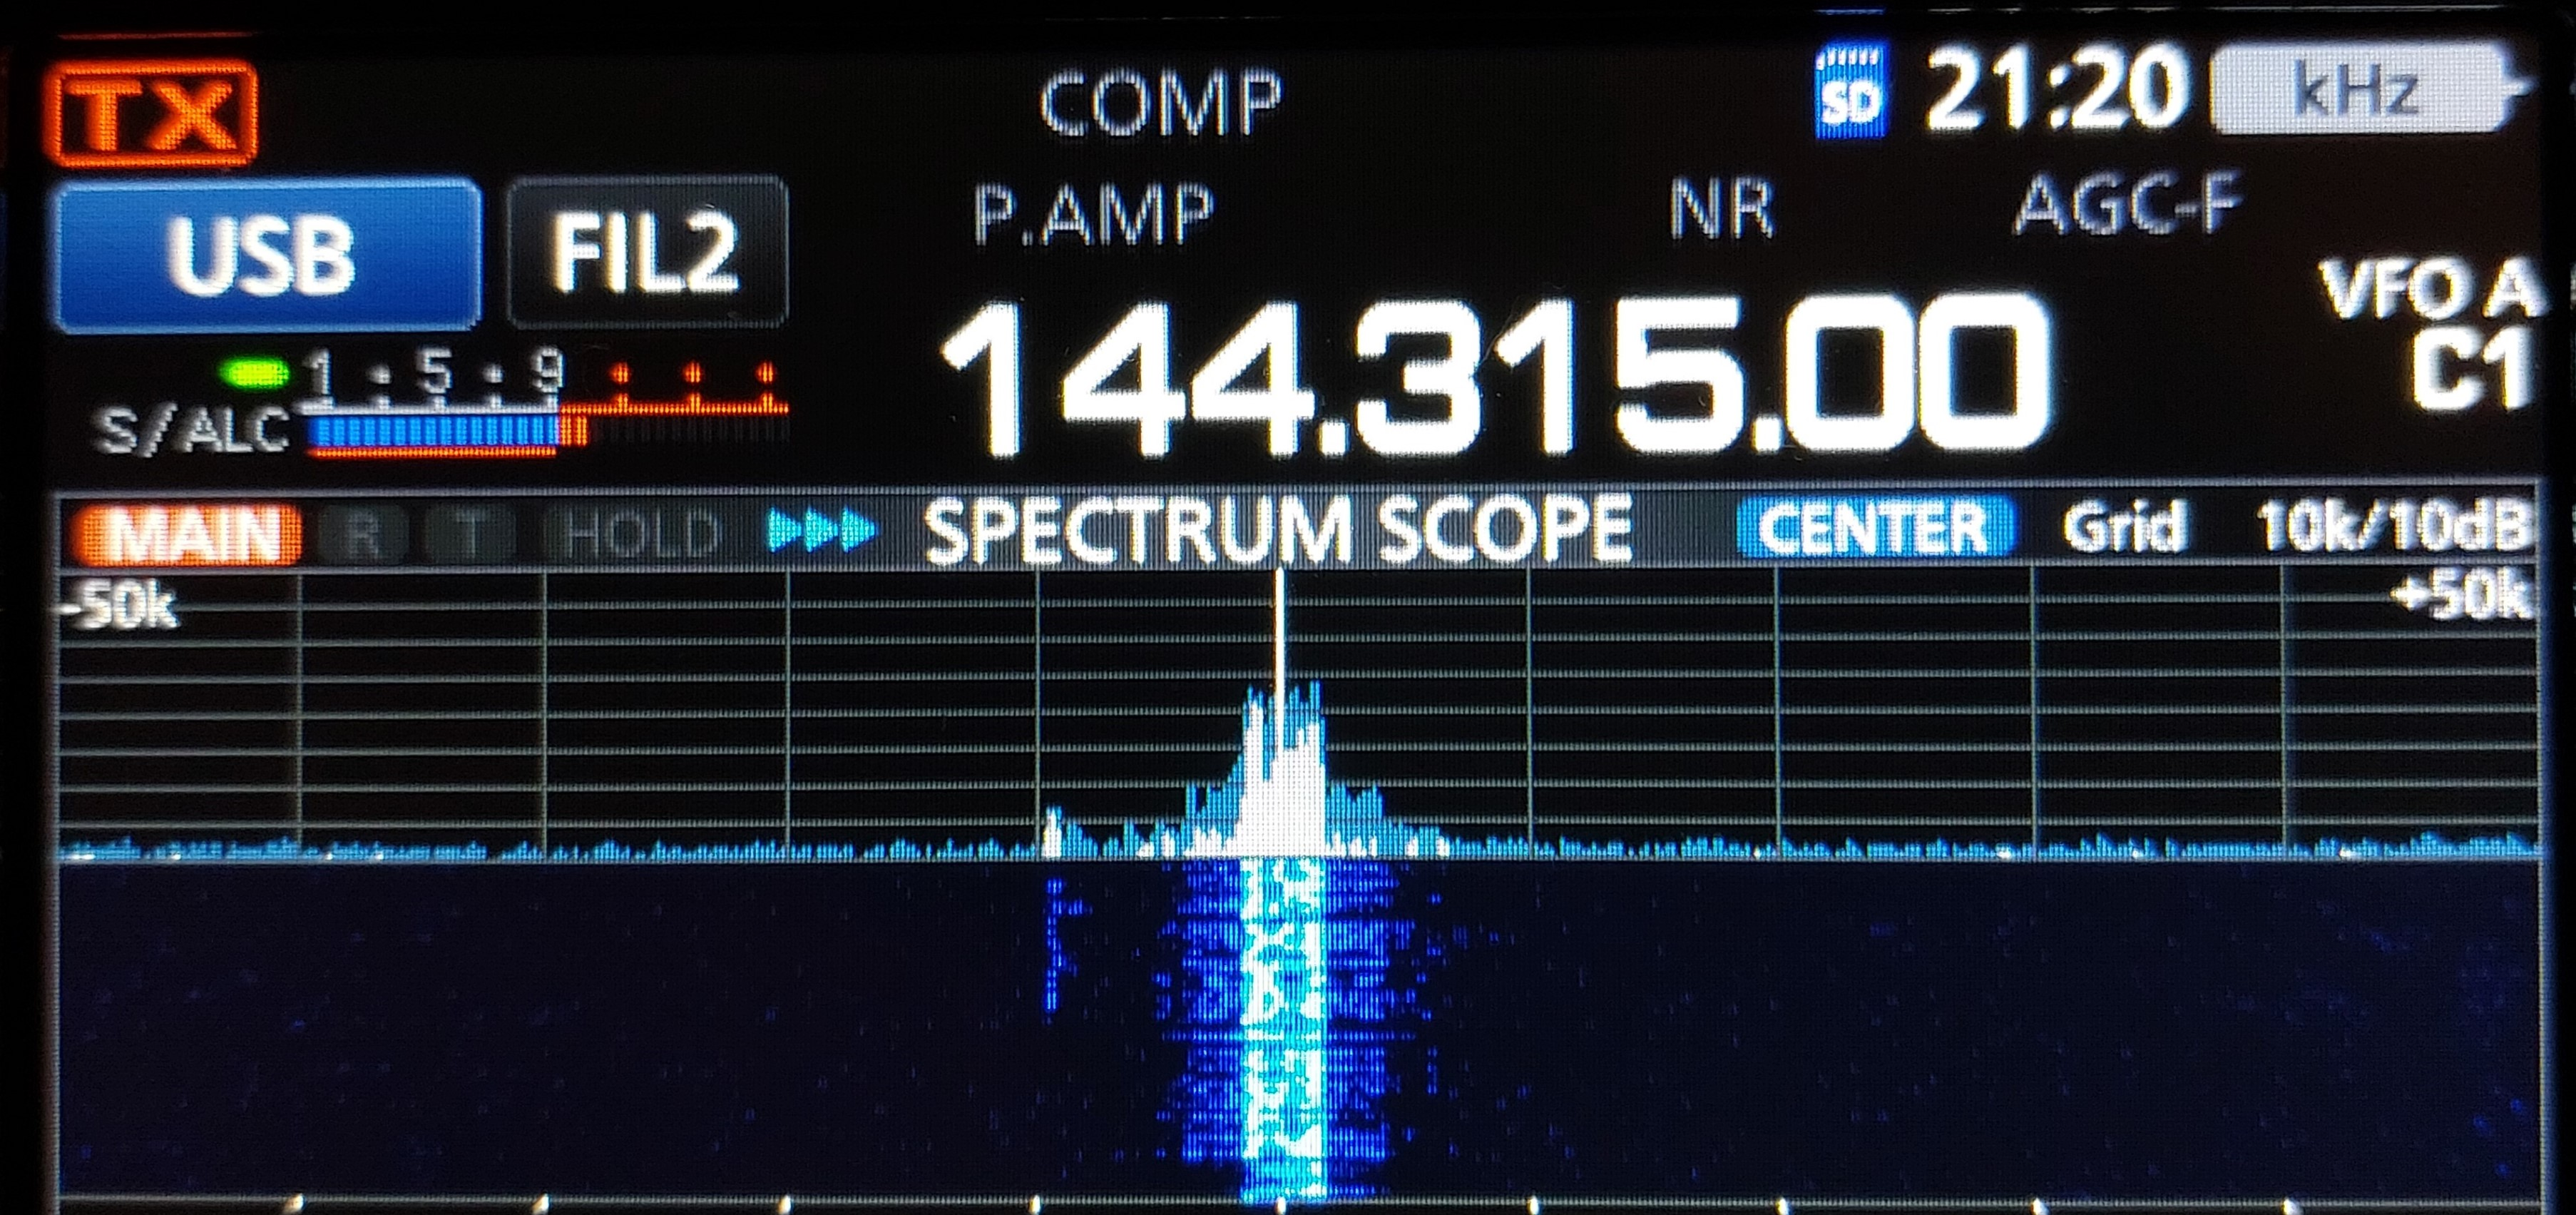
\includegraphics[width=0.85\textwidth]{foto/95}
    \caption{\scriptsize Display eines ICOM IC-9700 mit Frequenzanzeige, Amplitudenspektrum und Wasserfalldiagramm. Eine starke Station wird empfangen.}
    \label{n_wasserfall_starke_station}
\end{figure}

    \end{column}
   \begin{column}{0.48\textwidth}
       \begin{itemize}
  \item Moderne Funkgeräte
  \item Anzeige weiterer sendender Stationen ober- und unterhalb der eingestellten Frequenz
  \end{itemize}

   \end{column}
\end{columns}

\end{frame}

\begin{frame}
\frametitle{Amplitudenspektrum}
\begin{columns}
    \begin{column}{0.48\textwidth}
    
\begin{figure}
    \includegraphics[width=0.85\textwidth]{foto/135}
    \caption{\scriptsize Display eines ICOM IC-9700. Hervorgehoben ist das Amplitudenspektrum}
    \label{n_wasserfall_amplitudenspektrum}
\end{figure}

    \end{column}
   \begin{column}{0.48\textwidth}
       \begin{itemize}
  \item Amplitude umso höher je stärker das Signal ist
  \item Weitere Stationen sind im Amplitudenspektrum sichtbar
  \end{itemize}

   \end{column}
\end{columns}

\end{frame}

\begin{frame}
\frametitle{Wasserfalldiagramm}
\begin{columns}
    \begin{column}{0.48\textwidth}
    
\begin{figure}
    \includegraphics[width=0.85\textwidth]{foto/136}
    \caption{\scriptsize Display eines ICOM IC-9700. Hervorgehoben ist der Wasserfall}
    \label{n_wasserfall_wasserfall}
\end{figure}

    \end{column}
   \begin{column}{0.48\textwidth}
       \begin{itemize}
  \item Zeitlicher Verlauf auf senkrechter Achse
  \item Farbton oder Helligkeit zeigt die Stärke des Signals
  \item Läuft von oben nach unten durch
  \item Beginn und Ende einer Aussendung erkennbar
  \end{itemize}

   \end{column}
\end{columns}

\end{frame}

\begin{frame}
\only<1>{
\begin{PQuestion}{NF104}{Die Darstellung zeigt das Display eines Transceivers. Wie wird die Anzeige 3 bezeichnet?}{Power-Meter}
{Amplitudenspektrum}
{S-Meter}
{Wasserfalldiagramm}
{\DARCimage{1.0\linewidth}{578include}}\end{PQuestion}

}
\only<2>{
\begin{PQuestion}{NF104}{Die Darstellung zeigt das Display eines Transceivers. Wie wird die Anzeige 3 bezeichnet?}{Power-Meter}
{\textbf{\textcolor{DARCgreen}{Amplitudenspektrum}}}
{S-Meter}
{Wasserfalldiagramm}
{\DARCimage{1.0\linewidth}{578include}}\end{PQuestion}

}
\end{frame}

\begin{frame}
\only<1>{
\begin{PQuestion}{NF105}{Die Darstellung zeigt das Display eines Transceivers. Wie wird die Anzeige 4 bezeichnet?}{Regenbogendiagramm}
{Wasserfalldiagramm}
{SWR-Meter}
{Power-Meter}
{\DARCimage{1.0\linewidth}{578include}}\end{PQuestion}

}
\only<2>{
\begin{PQuestion}{NF105}{Die Darstellung zeigt das Display eines Transceivers. Wie wird die Anzeige 4 bezeichnet?}{Regenbogendiagramm}
{\textbf{\textcolor{DARCgreen}{Wasserfalldiagramm}}}
{SWR-Meter}
{Power-Meter}
{\DARCimage{1.0\linewidth}{578include}}\end{PQuestion}

}
\end{frame}

\begin{frame}
\only<1>{
\begin{PQuestion}{NF106}{Die Darstellung zeigt das Display eines Transceivers. Was wird im Wasserfalldiagramm dargestellt und wie erfolgt die Darstellung?}{Frequenz und Zeit auf den Achsen und Signalstärke als Farbton und/oder Helligkeit.}
{Frequenz und Signalstärke auf den Achsen und Zeit als Farbton und/oder Helligkeit.}
{Signalstärke und Zeit auf den Achsen und Frequenz als Farbton und/oder Helligkeit.}
{Signalstärke und Phase auf den Achsen und Zeit als Farbton und/oder Helligkeit.}
{\DARCimage{1.0\linewidth}{579include}}\end{PQuestion}

}
\only<2>{
\begin{PQuestion}{NF106}{Die Darstellung zeigt das Display eines Transceivers. Was wird im Wasserfalldiagramm dargestellt und wie erfolgt die Darstellung?}{\textbf{\textcolor{DARCgreen}{Frequenz und Zeit auf den Achsen und Signalstärke als Farbton und/oder Helligkeit.}}}
{Frequenz und Signalstärke auf den Achsen und Zeit als Farbton und/oder Helligkeit.}
{Signalstärke und Zeit auf den Achsen und Frequenz als Farbton und/oder Helligkeit.}
{Signalstärke und Phase auf den Achsen und Zeit als Farbton und/oder Helligkeit.}
{\DARCimage{1.0\linewidth}{579include}}\end{PQuestion}

}
\end{frame}

\begin{frame}
\frametitle{Unterschied Oszillogramm und Amplitudenspektrum}
\begin{itemize}
  \item Amplitudenspektrum zeigt horizontal Amplituden für verschiedene Frequenzen an
  \item Oszillogramm zeigt horizontal Amplituden zu verschiedenen Zeitpunkten an
  \end{itemize}
\end{frame}

\begin{frame}
\only<1>{
\begin{QQuestion}{NI401}{Was ist der Unterschied zwischen einem Oszillogramm und einem Amplitudenspektrum?}{Ein Oszillogramm zeigt den Strom und ein Amplitudenspektrum die Spannung eines Signals.}
{Ein Oszillogramm zeigt die Frequenzanteile und ein Amplitudenspektrum einen zeitlichen Verlauf eines Signals.}
{Ein Oszillogramm zeigt die Spannung und ein Amplitudenspektrum den Strom eines Signals.}
{Ein Oszillogramm zeigt einen zeitlichen Verlauf und ein Amplitudenspektrum die Frequenzanteile eines Signals.}
\end{QQuestion}

}
\only<2>{
\begin{QQuestion}{NI401}{Was ist der Unterschied zwischen einem Oszillogramm und einem Amplitudenspektrum?}{Ein Oszillogramm zeigt den Strom und ein Amplitudenspektrum die Spannung eines Signals.}
{Ein Oszillogramm zeigt die Frequenzanteile und ein Amplitudenspektrum einen zeitlichen Verlauf eines Signals.}
{Ein Oszillogramm zeigt die Spannung und ein Amplitudenspektrum den Strom eines Signals.}
{\textbf{\textcolor{DARCgreen}{Ein Oszillogramm zeigt einen zeitlichen Verlauf und ein Amplitudenspektrum die Frequenzanteile eines Signals.}}}
\end{QQuestion}

}
\end{frame}%ENDCONTENT


\section{Frequenzspektrum}
\label{section:frequenzspektrum}
\begin{frame}%STARTCONTENT

\begin{figure}
    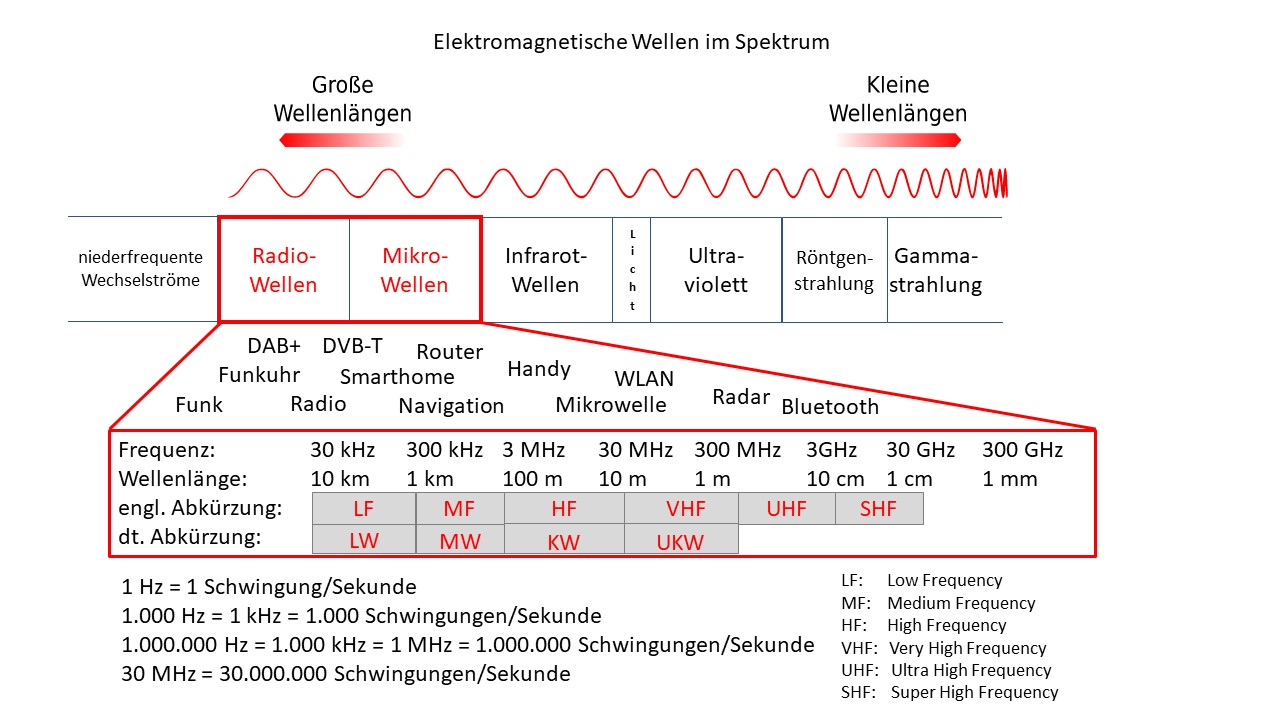
\includegraphics[width=0.85\textwidth]{foto/94}
    \caption{\scriptsize Spektrum der elektromagnetischen Wellen}
    \label{n_frequenzspektrum}
\end{figure}

\end{frame}

\begin{frame}\begin{table}
\begin{DARCtabular}{rcrXl}
     \qty{30}{\kilo\hertz}  & --  & \qty{300}{\kilo\hertz}  & Low Frequency  & LF   \\
      &  &  & (Langwelle)  & (LW)   \\
     \qty{300}{\kilo\hertz}  & --  & \qty{3000}{\kilo\hertz}  & Medium Frequency  & MF   \\
      &  &  & (Mittelwelle)  & (MW)   \\
     \qty{3}{\mega\hertz}  & --  & \qty{30}{\mega\hertz}  & \emph{High Frequency}  & \emph{HF}   \\
      &  &  & Short Wave  & SW   \\
      &  &  & (Kurzwelle)  & (KW)   \\
     \qty{30}{\mega\hertz}  & --  & \qty{300}{\mega\hertz}  & \emph{Very High Frequency}  & \emph{VHF}   \\
      &  &  & (Ultrakurzwelle)  & (UKW)   \\
     \qty{300}{\mega\hertz}  & --  & \qty{3000}{\mega\hertz}  & \emph{Ultra High Frequency}  & \emph{UHF}   \\
      &  &  & (Dezimeterwelle)  &   \\
     \qty{3}{\giga\hertz}  & --  & \qty{30}{\giga\hertz}  & Super High Frequency  & SHF   \\
     \qty{30}{\giga\hertz}  & --  & \qty{300}{\giga\hertz}  & Extemely High Frequency  & EHF   \\
\end{DARCtabular}
\caption{Die Frequenzbereiche von 30 kHz bis 300 GHz und ihre üblichen Bezeichnungen.}
\label{n_frequenzspektrum_bereiche}
\end{table}
\end{frame}

\begin{frame}
\only<1>{
\begin{QQuestion}{BC104}{Wie wird der Frequenzbereich von \qtyrange{3}{30}{\MHz} bezeichnet?}{Medium Frequency (MF) oder Mittelwelle (MW)}
{Very High Frequency (VHF) oder Ultrakurzwelle (UKW)}
{Ultra High Frequency (UHF) oder Dezimeterwelle}
{High Frequency (HF), Short Wave (SW) oder Kurzwelle (KW)}
\end{QQuestion}

}
\only<2>{
\begin{QQuestion}{BC104}{Wie wird der Frequenzbereich von \qtyrange{3}{30}{\MHz} bezeichnet?}{Medium Frequency (MF) oder Mittelwelle (MW)}
{Very High Frequency (VHF) oder Ultrakurzwelle (UKW)}
{Ultra High Frequency (UHF) oder Dezimeterwelle}
{\textbf{\textcolor{DARCgreen}{High Frequency (HF), Short Wave (SW) oder Kurzwelle (KW)}}}
\end{QQuestion}

}
\end{frame}

\begin{frame}
\only<1>{
\begin{QQuestion}{BC105}{Wie wird der Frequenzbereich zwischen \qtyrange{30}{300}{\MHz} bezeichnet?}{High Frequency (HF), Short Wave (SW) oder Kurzwelle (KW)}
{Ultra High Frequency (UHF) oder Dezimeterwelle}
{Very High Frequency (VHF) oder Ultrakurzwelle (UKW)}
{Medium Frequency (MF) oder Mittelwelle (MW)}
\end{QQuestion}

}
\only<2>{
\begin{QQuestion}{BC105}{Wie wird der Frequenzbereich zwischen \qtyrange{30}{300}{\MHz} bezeichnet?}{High Frequency (HF), Short Wave (SW) oder Kurzwelle (KW)}
{Ultra High Frequency (UHF) oder Dezimeterwelle}
{\textbf{\textcolor{DARCgreen}{Very High Frequency (VHF) oder Ultrakurzwelle (UKW)}}}
{Medium Frequency (MF) oder Mittelwelle (MW)}
\end{QQuestion}

}
\end{frame}

\begin{frame}
\only<1>{
\begin{QQuestion}{BC106}{Wie wird der Frequenzbereich zwischen \qtyrange{300}{3000}{\MHz} bezeichnet?}{Very High Frequency (VHF) oder Ultrakurzwelle (UKW)}
{Ultra High Frequency (UHF) oder Dezimeterwelle}
{High Frequency (HF), Short Wave (SW) oder Kurzwelle (KW)}
{Medium Frequency (MF) oder Mittelwelle (MW)}
\end{QQuestion}

}
\only<2>{
\begin{QQuestion}{BC106}{Wie wird der Frequenzbereich zwischen \qtyrange{300}{3000}{\MHz} bezeichnet?}{Very High Frequency (VHF) oder Ultrakurzwelle (UKW)}
{\textbf{\textcolor{DARCgreen}{Ultra High Frequency (UHF) oder Dezimeterwelle}}}
{High Frequency (HF), Short Wave (SW) oder Kurzwelle (KW)}
{Medium Frequency (MF) oder Mittelwelle (MW)}
\end{QQuestion}

}
\end{frame}

\begin{frame}
\only<1>{
\begin{QQuestion}{BC101}{Wie wird der Frequenzbereich bezeichnet, in dem sich das \qty{10}{\m}-Band befindet?}{Ultra High Frequency (UHF) oder Dezimeterwelle}
{Very High Frequency (VHF) oder Ultrakurzwelle (UKW)}
{High Frequency (HF), Short Wave (SW) oder Kurzwelle (KW)}
{Medium Frequency (MF) oder Mittelwelle (MW)}
\end{QQuestion}

}
\only<2>{
\begin{QQuestion}{BC101}{Wie wird der Frequenzbereich bezeichnet, in dem sich das \qty{10}{\m}-Band befindet?}{Ultra High Frequency (UHF) oder Dezimeterwelle}
{Very High Frequency (VHF) oder Ultrakurzwelle (UKW)}
{\textbf{\textcolor{DARCgreen}{High Frequency (HF), Short Wave (SW) oder Kurzwelle (KW)}}}
{Medium Frequency (MF) oder Mittelwelle (MW)}
\end{QQuestion}

}

\end{frame}

\begin{frame}
\only<1>{
\begin{QQuestion}{BC102}{Wie wird der Frequenzbereich bezeichnet, in dem sich das \qty{2}{\m}-Band befindet?}{High Frequency (HF), Short Wave (SW) oder Kurzwelle (KW)}
{Ultra High Frequency (UHF) oder Dezimeterwelle}
{Very High Frequency (VHF) oder Ultrakurzwelle (UKW)}
{Medium Frequency (MF) oder Mittelwelle (MW)}
\end{QQuestion}

}
\only<2>{
\begin{QQuestion}{BC102}{Wie wird der Frequenzbereich bezeichnet, in dem sich das \qty{2}{\m}-Band befindet?}{High Frequency (HF), Short Wave (SW) oder Kurzwelle (KW)}
{Ultra High Frequency (UHF) oder Dezimeterwelle}
{\textbf{\textcolor{DARCgreen}{Very High Frequency (VHF) oder Ultrakurzwelle (UKW)}}}
{Medium Frequency (MF) oder Mittelwelle (MW)}
\end{QQuestion}

}

\end{frame}

\begin{frame}
\only<1>{
\begin{QQuestion}{BC103}{Wie wird der Frequenzbereich bezeichnet, in dem sich das \qty{70}{\cm}-Band befindet?}{Ultra High Frequency (UHF) oder Dezimeterwelle}
{Very High Frequency (VHF) oder Ultrakurzwelle (UKW)}
{High Frequency (HF), Short Wave (SW) oder Kurzwelle (KW)}
{Medium Frequency (MF) oder Mittelwelle (MW)}
\end{QQuestion}

}
\only<2>{
\begin{QQuestion}{BC103}{Wie wird der Frequenzbereich bezeichnet, in dem sich das \qty{70}{\cm}-Band befindet?}{\textbf{\textcolor{DARCgreen}{Ultra High Frequency (UHF) oder Dezimeterwelle}}}
{Very High Frequency (VHF) oder Ultrakurzwelle (UKW)}
{High Frequency (HF), Short Wave (SW) oder Kurzwelle (KW)}
{Medium Frequency (MF) oder Mittelwelle (MW)}
\end{QQuestion}

}

\end{frame}%ENDCONTENT


\section{Frequenzzuteilung}
\label{section:frequenzzuteilung}
\begin{frame}%STARTCONTENT
\begin{itemize}
  \item Jede Frequenznutzung bedarf einer vorherigen \emph{Frequenzzuteilung}
  \item Verankert im Telekommunikationsgesetz (TKG)
  \item Einzelzuteilung oder Allgemeinzuteilung
  \end{itemize}

\end{frame}

\begin{frame}\begin{itemize}
  \item Amateurfunk darf nur auf den zugeteilten Frequenzen durchgeführt werden
  \item Frequenzbereiche sind zwar international vereinbart
  \item \emph{Aber} die nationalen Bestimmungen sind maßgebend
  \end{itemize}
\end{frame}

\begin{frame}
\only<1>{
\begin{QQuestion}{VE102}{Bedarf jede Frequenznutzung einer Frequenzzuteilung?}{Eine Frequenznutzung ist auch ohne Frequenzzuteilung zulässig.}
{Erst ab \qty{0,1}{\W} ist eine Frequenzzuteilung erforderlich.}
{Es gibt Ausnahmen von der Notwendigkeit zur Frequenzzuteilung, z.~B. die ISM-Frequenzen.}
{Jede Frequenznutzung bedarf einer vorherigen Frequenzzuteilung.}
\end{QQuestion}

}
\only<2>{
\begin{QQuestion}{VE102}{Bedarf jede Frequenznutzung einer Frequenzzuteilung?}{Eine Frequenznutzung ist auch ohne Frequenzzuteilung zulässig.}
{Erst ab \qty{0,1}{\W} ist eine Frequenzzuteilung erforderlich.}
{Es gibt Ausnahmen von der Notwendigkeit zur Frequenzzuteilung, z.~B. die ISM-Frequenzen.}
{\textbf{\textcolor{DARCgreen}{Jede Frequenznutzung bedarf einer vorherigen Frequenzzuteilung.}}}
\end{QQuestion}

}
\end{frame}

\begin{frame}
\only<1>{
\begin{QQuestion}{VD701}{Darf ein Funkamateur in Deutschland alle in den Radio Regulations (RR) für den Amateurfunkdienst zugewiesenen Frequenzbereiche benutzen?}{Nein, es dürfen nur Frequenzen genutzt werden, die durch nationale Regelungen umgesetzt wurden.}
{Ja, weil die internationalen Regelungen der Radio Regulations (RR) auch in Deutschland gelten.}
{Ja, wenn der Betrieb bei der Bundesnetzagentur vorher angemeldet wurde.}
{Nein, die in Deutschland zulässigen Frequenzbereiche ergeben sich aus der Frequenznutzungsplanaufstellungsverordnung.}
\end{QQuestion}

}
\only<2>{
\begin{QQuestion}{VD701}{Darf ein Funkamateur in Deutschland alle in den Radio Regulations (RR) für den Amateurfunkdienst zugewiesenen Frequenzbereiche benutzen?}{\textbf{\textcolor{DARCgreen}{Nein, es dürfen nur Frequenzen genutzt werden, die durch nationale Regelungen umgesetzt wurden.}}}
{Ja, weil die internationalen Regelungen der Radio Regulations (RR) auch in Deutschland gelten.}
{Ja, wenn der Betrieb bei der Bundesnetzagentur vorher angemeldet wurde.}
{Nein, die in Deutschland zulässigen Frequenzbereiche ergeben sich aus der Frequenznutzungsplanaufstellungsverordnung.}
\end{QQuestion}

}
\end{frame}

\begin{frame}
\only<1>{
\begin{QQuestion}{VC110}{Was gilt für Funkamateure hinsichtlich der Frequenznutzung? Ein Funkamateur darf mit seiner Amateurfunkstelle~...}{beliebige Frequenzen nutzen, sofern keine anderen Funkdienste gestört werden.}
{auf allen für seine ITU-Region zugelassenen Frequenzen senden.}
{auf den für den Amateurfunkdienst ausgewiesenen Frequenzen senden.}
{im Rahmen einer Notfunkübung auch auf nicht für den Amateurfunkdienst ausgewiesenen Frequenzen senden.}
\end{QQuestion}

}
\only<2>{
\begin{QQuestion}{VC110}{Was gilt für Funkamateure hinsichtlich der Frequenznutzung? Ein Funkamateur darf mit seiner Amateurfunkstelle~...}{beliebige Frequenzen nutzen, sofern keine anderen Funkdienste gestört werden.}
{auf allen für seine ITU-Region zugelassenen Frequenzen senden.}
{\textbf{\textcolor{DARCgreen}{auf den für den Amateurfunkdienst ausgewiesenen Frequenzen senden.}}}
{im Rahmen einer Notfunkübung auch auf nicht für den Amateurfunkdienst ausgewiesenen Frequenzen senden.}
\end{QQuestion}

}
\end{frame}

\begin{frame}
\frametitle{Frequenzbereiche für den Amateurfunkdienst}
\begin{itemize}
  \item Sind in Deutschland in der Anlage 1 der \emph{Verordnung über den Amateurfunk (AFuV)} geregelt
  \item Senden nur auf den der Zeugnisklasse zugewiesenen Frequenzen
  \item Weitere einzuhaltende Nutzungsbestimmungen
  \item Es gibt ergänzende bindende Verfügungen und Mitteilungen
  \item Werden im Amtsblatt und auf der Webseite der Bundesnetzagentur (BNetzA) veröffentlicht
  \end{itemize}
\end{frame}

\begin{frame}
\begin{figure}
    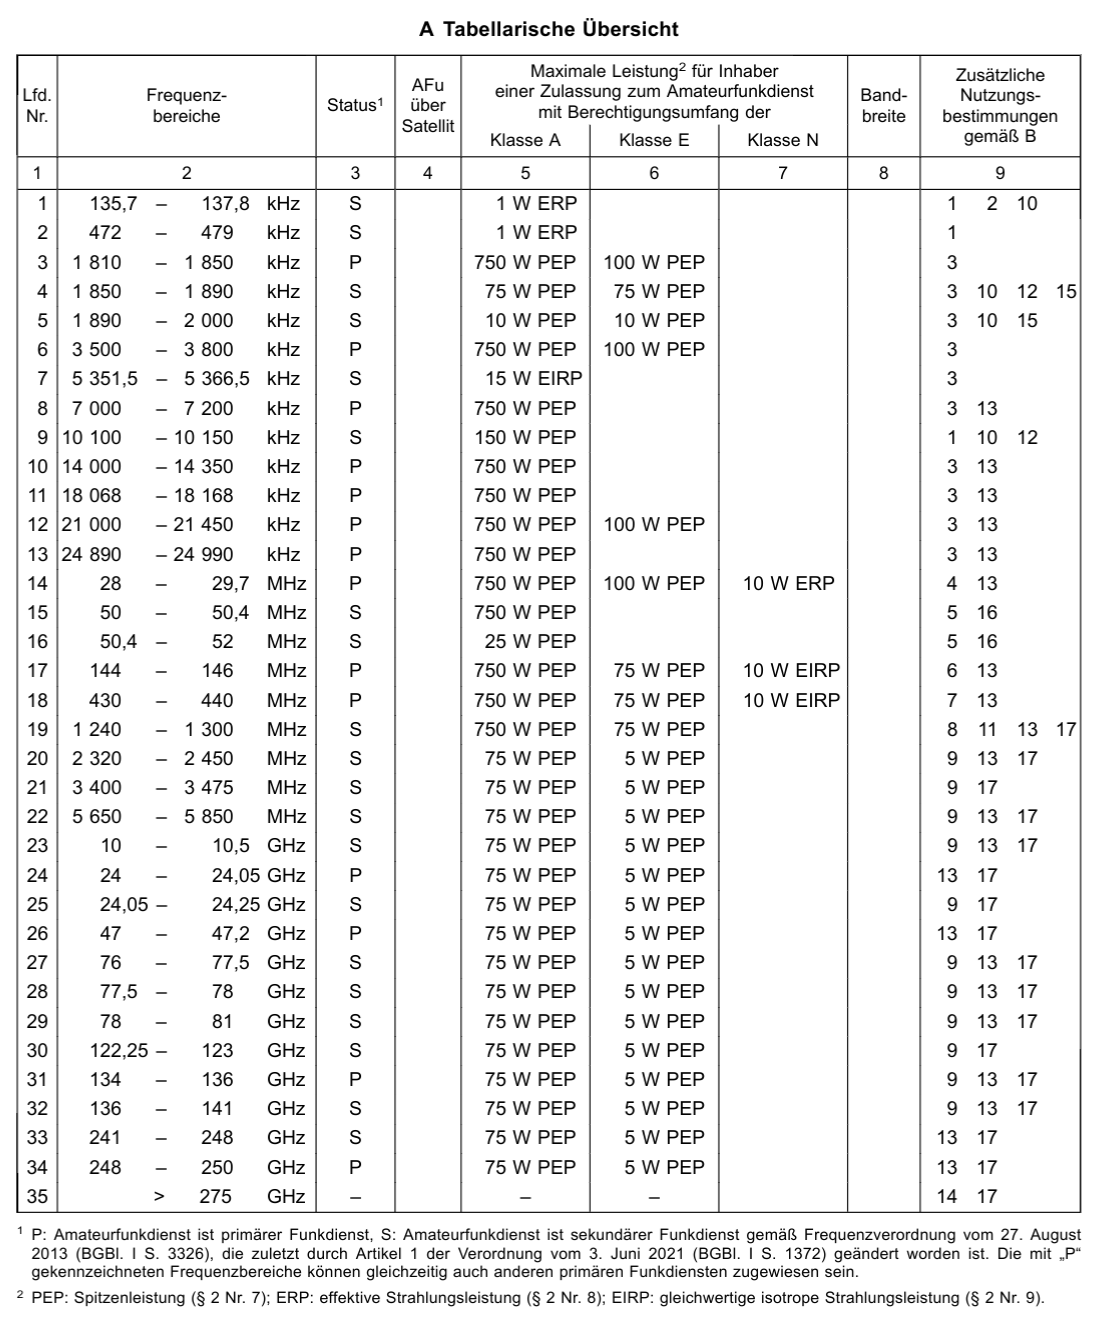
\includegraphics[width=0.85\textwidth]{foto/99}
    \caption{\scriptsize Tabellarische Übersicht, Anlage 1, AFuV (Korrektur in den Leistungen für Klasse~N notwendig)}
    \label{n_frequenzbereiche_afuv_anlage_1}
\end{figure}

\end{frame}

\begin{frame}
\only<1>{
\begin{QQuestion}{VD101}{Wo kann der Funkamateur nachschlagen, welche Frequenzbereiche er entsprechend seiner Zeugnisklasse in Deutschland nutzen darf?}{In der Anlage zur Frequenzverordnung (FreqV) und den dazugehörigen Mitteilungen der BNetzA}
{In den Radio Regulations (RR)}
{Im Amateurfunkgesetz (AFuG)}
{In der Anlage 1 der Amateurfunkverordnung (AFuV) und ggf. weiteren Mitteilungen der BNetzA}
\end{QQuestion}

}
\only<2>{
\begin{QQuestion}{VD101}{Wo kann der Funkamateur nachschlagen, welche Frequenzbereiche er entsprechend seiner Zeugnisklasse in Deutschland nutzen darf?}{In der Anlage zur Frequenzverordnung (FreqV) und den dazugehörigen Mitteilungen der BNetzA}
{In den Radio Regulations (RR)}
{Im Amateurfunkgesetz (AFuG)}
{\textbf{\textcolor{DARCgreen}{In der Anlage 1 der Amateurfunkverordnung (AFuV) und ggf. weiteren Mitteilungen der BNetzA}}}
\end{QQuestion}

}
\end{frame}

\begin{frame}
\only<1>{
\begin{QQuestion}{VD702}{Wo sind die für den Amateurfunkdienst in Deutschland ausgewiesenen Frequenzbereiche und die zugehörigen ausführlichen Nutzungsbedingungen zu finden?}{In Artikel~5 der Radio Regulations (RR)}
{In der Anlage 1 der Amateurfunkverordnung (AFuV) und ggf. weiteren Mitteilungen der BNetzA}
{Im Frequenzplan (FreqP)}
{In der Anlage zur Frequenzverordnung (FreqV)}
\end{QQuestion}

}
\only<2>{
\begin{QQuestion}{VD702}{Wo sind die für den Amateurfunkdienst in Deutschland ausgewiesenen Frequenzbereiche und die zugehörigen ausführlichen Nutzungsbedingungen zu finden?}{In Artikel~5 der Radio Regulations (RR)}
{\textbf{\textcolor{DARCgreen}{In der Anlage 1 der Amateurfunkverordnung (AFuV) und ggf. weiteren Mitteilungen der BNetzA}}}
{Im Frequenzplan (FreqP)}
{In der Anlage zur Frequenzverordnung (FreqV)}
\end{QQuestion}

}
\end{frame}%ENDCONTENT


\section{Amateurfunkbänder}
\label{section:amateurfunkbaender}
\begin{frame}%STARTCONTENT
\begin{itemize}
  \item Funkamateure müssen wissen, welche Frequenzen genutzt werden dürfen
  \item Lässt sich aus Anlage 1 AfuV ablesen
  \item Die Anlage 1 liegt in der Prüfung als Hilfsmittel bereit
  \end{itemize}
\end{frame}

\begin{frame}
\begin{figure}
    \DARCimage{0.85\linewidth}{829include}
    \caption{\scriptsize Frequenzbereiche im Amateurfunk unter \qty{300}{\mega\hertz}}
    \label{amateuerfunkbaender_2}
\end{figure}

\end{frame}

\begin{frame}
\begin{figure}
    \DARCimage{0.85\linewidth}{830include}
    \caption{\scriptsize Frequenzbereiche im Amateurfunk über \qty{300}{\mega\hertz}}
    \label{amateuerfunkbaender_1}
\end{figure}

\end{frame}

\begin{frame}
\only<1>{
\begin{QQuestion}{VD709}{Welche Antwort enthält die richtige Anfangs- und Endfrequenz für das \qty{160}{\m}-Amateurfunkband in Deutschland?}{\qtyrange{1810}{2000}{\kHz}}
{\qtyrange{1805}{1850}{\kHz}}
{\qtyrange{1800}{1900}{\kHz}}
{\qtyrange{1800}{1990}{\kHz}}
\end{QQuestion}

}
\only<2>{
\begin{QQuestion}{VD709}{Welche Antwort enthält die richtige Anfangs- und Endfrequenz für das \qty{160}{\m}-Amateurfunkband in Deutschland?}{\textbf{\textcolor{DARCgreen}{\qtyrange{1810}{2000}{\kHz}}}}
{\qtyrange{1805}{1850}{\kHz}}
{\qtyrange{1800}{1900}{\kHz}}
{\qtyrange{1800}{1990}{\kHz}}
\end{QQuestion}

}
\end{frame}

\begin{frame}
\only<1>{
\begin{QQuestion}{VD710}{Welche Antwort enthält die richtige Anfangs- und Endfrequenz für das \qty{80}{\m}-Amateurfunkband in Deutschland?}{\qtyrange{3,8}{4}{\MHz}}
{\qtyrange{3,5}{3,6}{\MHz}}
{\qtyrange{3,8}{3,9}{\MHz}}
{\qtyrange{3,5}{3,8}{\MHz}}
\end{QQuestion}

}
\only<2>{
\begin{QQuestion}{VD710}{Welche Antwort enthält die richtige Anfangs- und Endfrequenz für das \qty{80}{\m}-Amateurfunkband in Deutschland?}{\qtyrange{3,8}{4}{\MHz}}
{\qtyrange{3,5}{3,6}{\MHz}}
{\qtyrange{3,8}{3,9}{\MHz}}
{\textbf{\textcolor{DARCgreen}{\qtyrange{3,5}{3,8}{\MHz}}}}
\end{QQuestion}

}
\end{frame}

\begin{frame}
\only<1>{
\begin{QQuestion}{VD711}{Welche Antwort enthält die richtige Anfangs- und Endfrequenz für das \qty{40}{\m}-Amateurfunkband in Deutschland?}{\qtyrange{7}{7,3}{\MHz}}
{\qtyrange{7,1}{7,3}{\MHz}}
{\qtyrange{7}{7,2}{\MHz}}
{\qtyrange{7,1}{7,5}{\MHz}}
\end{QQuestion}

}
\only<2>{
\begin{QQuestion}{VD711}{Welche Antwort enthält die richtige Anfangs- und Endfrequenz für das \qty{40}{\m}-Amateurfunkband in Deutschland?}{\qtyrange{7}{7,3}{\MHz}}
{\qtyrange{7,1}{7,3}{\MHz}}
{\textbf{\textcolor{DARCgreen}{\qtyrange{7}{7,2}{\MHz}}}}
{\qtyrange{7,1}{7,5}{\MHz}}
\end{QQuestion}

}
\end{frame}

\begin{frame}
\only<1>{
\begin{QQuestion}{VD712}{Welche Antwort enthält die richtige Anfangs- und Endfrequenz für das \qty{30}{\m}-Amateurfunkband in Deutschland?}{\qtyrange{10}{10,25}{\MHz}}
{\qtyrange{10,1}{10,25}{\MHz}}
{\qtyrange{10}{10,15}{\MHz}}
{\qtyrange{10,1}{10,15}{\MHz}}
\end{QQuestion}

}
\only<2>{
\begin{QQuestion}{VD712}{Welche Antwort enthält die richtige Anfangs- und Endfrequenz für das \qty{30}{\m}-Amateurfunkband in Deutschland?}{\qtyrange{10}{10,25}{\MHz}}
{\qtyrange{10,1}{10,25}{\MHz}}
{\qtyrange{10}{10,15}{\MHz}}
{\textbf{\textcolor{DARCgreen}{\qtyrange{10,1}{10,15}{\MHz}}}}
\end{QQuestion}

}
\end{frame}

\begin{frame}
\only<1>{
\begin{QQuestion}{VD713}{Welche Antwort enthält die richtige Anfangs- und Endfrequenz für das \qty{20}{\m}-Amateurfunkband in Deutschland?}{\qtyrange{14}{14,35}{\MHz}}
{\qtyrange{14}{14,45}{\MHz}}
{\qtyrange{14}{14,5}{\MHz}}
{\qtyrange{14}{15}{\MHz}}
\end{QQuestion}

}
\only<2>{
\begin{QQuestion}{VD713}{Welche Antwort enthält die richtige Anfangs- und Endfrequenz für das \qty{20}{\m}-Amateurfunkband in Deutschland?}{\textbf{\textcolor{DARCgreen}{\qtyrange{14}{14,35}{\MHz}}}}
{\qtyrange{14}{14,45}{\MHz}}
{\qtyrange{14}{14,5}{\MHz}}
{\qtyrange{14}{15}{\MHz}}
\end{QQuestion}

}
\end{frame}

\begin{frame}
\only<1>{
\begin{QQuestion}{VD714}{Welche Antwort enthält die richtige Anfangs- und Endfrequenz für das \qty{17}{\m}-Amateurfunkband in Deutschland?}{\qtyrange{18,1}{18,158}{\MHz}}
{\qtyrange{18,068}{18,168}{\MHz}}
{\qtyrange{18,89}{18,99}{\MHz}}
{\qtyrange{18,68}{19,99}{\MHz}}
\end{QQuestion}

}
\only<2>{
\begin{QQuestion}{VD714}{Welche Antwort enthält die richtige Anfangs- und Endfrequenz für das \qty{17}{\m}-Amateurfunkband in Deutschland?}{\qtyrange{18,1}{18,158}{\MHz}}
{\textbf{\textcolor{DARCgreen}{\qtyrange{18,068}{18,168}{\MHz}}}}
{\qtyrange{18,89}{18,99}{\MHz}}
{\qtyrange{18,68}{19,99}{\MHz}}
\end{QQuestion}

}
\end{frame}

\begin{frame}
\only<1>{
\begin{QQuestion}{VD715}{Welche Antwort enthält die richtige Anfangs- und Endfrequenz für das \qty{15}{\m}-Amateurfunkband in Deutschland?}{\qtyrange{21}{21,7}{\MHz}}
{\qtyrange{21}{21,35}{\MHz}}
{\qtyrange{21}{21,5}{\MHz}}
{\qtyrange{21}{21,45}{\MHz}}
\end{QQuestion}

}
\only<2>{
\begin{QQuestion}{VD715}{Welche Antwort enthält die richtige Anfangs- und Endfrequenz für das \qty{15}{\m}-Amateurfunkband in Deutschland?}{\qtyrange{21}{21,7}{\MHz}}
{\qtyrange{21}{21,35}{\MHz}}
{\qtyrange{21}{21,5}{\MHz}}
{\textbf{\textcolor{DARCgreen}{\qtyrange{21}{21,45}{\MHz}}}}
\end{QQuestion}

}
\end{frame}

\begin{frame}
\only<1>{
\begin{QQuestion}{VD716}{Welche Antwort enthält die richtige Anfangs- und Endfrequenz für das \qty{12}{\m}-Amateurfunkband in Deutschland?}{\qtyrange{24,89}{24,99}{\MHz}}
{\qtyrange{24,89}{25,168}{\MHz}}
{\qtyrange{24,168}{24,99}{\MHz}}
{\qtyrange{24,068}{24,168}{\MHz}}
\end{QQuestion}

}
\only<2>{
\begin{QQuestion}{VD716}{Welche Antwort enthält die richtige Anfangs- und Endfrequenz für das \qty{12}{\m}-Amateurfunkband in Deutschland?}{\textbf{\textcolor{DARCgreen}{\qtyrange{24,89}{24,99}{\MHz}}}}
{\qtyrange{24,89}{25,168}{\MHz}}
{\qtyrange{24,168}{24,99}{\MHz}}
{\qtyrange{24,068}{24,168}{\MHz}}
\end{QQuestion}

}
\end{frame}

\begin{frame}
\only<1>{
\begin{QQuestion}{VD717}{Welche Antwort enthält die richtige Anfangs- und Endfrequenz für das \qty{10}{\m}-Amateurfunkband in Deutschland?}{\qtyrange{28}{29,7}{\MHz}}
{\qtyrange{28}{29}{\MHz}}
{\qtyrange{28}{30,7}{\MHz}}
{\qtyrange{28}{32}{\MHz}}
\end{QQuestion}

}
\only<2>{
\begin{QQuestion}{VD717}{Welche Antwort enthält die richtige Anfangs- und Endfrequenz für das \qty{10}{\m}-Amateurfunkband in Deutschland?}{\textbf{\textcolor{DARCgreen}{\qtyrange{28}{29,7}{\MHz}}}}
{\qtyrange{28}{29}{\MHz}}
{\qtyrange{28}{30,7}{\MHz}}
{\qtyrange{28}{32}{\MHz}}
\end{QQuestion}

}
\end{frame}

\begin{frame}
\only<1>{
\begin{QQuestion}{VD718}{Welche Antwort enthält die richtige Anfangs- und Endfrequenz für das \qty{6}{\m}-Amateurfunkband in Deutschland?}{\qtyrange{50,0}{54,0}{\MHz}}
{\qtyrange{50,0}{52,00}{\MHz}}
{\qtyrange{50,8}{51,8}{\MHz}}
{\qtyrange{51,08}{52,00}{\MHz}}
\end{QQuestion}

}
\only<2>{
\begin{QQuestion}{VD718}{Welche Antwort enthält die richtige Anfangs- und Endfrequenz für das \qty{6}{\m}-Amateurfunkband in Deutschland?}{\qtyrange{50,0}{54,0}{\MHz}}
{\textbf{\textcolor{DARCgreen}{\qtyrange{50,0}{52,00}{\MHz}}}}
{\qtyrange{50,8}{51,8}{\MHz}}
{\qtyrange{51,08}{52,00}{\MHz}}
\end{QQuestion}

}
\end{frame}

\begin{frame}
\only<1>{
\begin{QQuestion}{VD719}{Welche Antwort enthält die richtige Anfangs- und Endfrequenz für das \qty{2}{\m}-Amateurfunkband in Deutschland?}{\qtyrange{140}{148}{\MHz}}
{\qtyrange{144}{148}{\MHz}}
{\qtyrange{140}{146}{\MHz}}
{\qtyrange{144}{146}{\MHz}}
\end{QQuestion}

}
\only<2>{
\begin{QQuestion}{VD719}{Welche Antwort enthält die richtige Anfangs- und Endfrequenz für das \qty{2}{\m}-Amateurfunkband in Deutschland?}{\qtyrange{140}{148}{\MHz}}
{\qtyrange{144}{148}{\MHz}}
{\qtyrange{140}{146}{\MHz}}
{\textbf{\textcolor{DARCgreen}{\qtyrange{144}{146}{\MHz}}}}
\end{QQuestion}

}
\end{frame}

\begin{frame}
\only<1>{
\begin{QQuestion}{VD720}{Welche Antwort enthält die richtige Anfangs- und Endfrequenz für das \qty{70}{\cm}-Amateurfunkband in Deutschland? }{\qtyrange{430}{440}{\MHz}}
{\qtyrange{430}{438}{\MHz}}
{\qtyrange{432}{440}{\MHz}}
{\qtyrange{432}{438}{\MHz}}
\end{QQuestion}

}
\only<2>{
\begin{QQuestion}{VD720}{Welche Antwort enthält die richtige Anfangs- und Endfrequenz für das \qty{70}{\cm}-Amateurfunkband in Deutschland? }{\textbf{\textcolor{DARCgreen}{\qtyrange{430}{440}{\MHz}}}}
{\qtyrange{430}{438}{\MHz}}
{\qtyrange{432}{440}{\MHz}}
{\qtyrange{432}{438}{\MHz}}
\end{QQuestion}

}
\end{frame}

\begin{frame}
\only<1>{
\begin{QQuestion}{VD721}{Welche Antwort enthält die richtige Anfangs- und Endfrequenz für das \qty{23}{\cm}-Amateurfunkband in Deutschland?}{\qtyrange{1240}{1300}{\MHz}}
{\qtyrange{1240}{1290}{\MHz}}
{\qtyrange{1220}{1300}{\MHz}}
{\qtyrange{1220}{1290}{\MHz}}
\end{QQuestion}

}
\only<2>{
\begin{QQuestion}{VD721}{Welche Antwort enthält die richtige Anfangs- und Endfrequenz für das \qty{23}{\cm}-Amateurfunkband in Deutschland?}{\textbf{\textcolor{DARCgreen}{\qtyrange{1240}{1300}{\MHz}}}}
{\qtyrange{1240}{1290}{\MHz}}
{\qtyrange{1220}{1300}{\MHz}}
{\qtyrange{1220}{1290}{\MHz}}
\end{QQuestion}

}
\end{frame}

\begin{frame}
\only<1>{
\begin{QQuestion}{VD722}{Welche Antwort enthält die richtige Anfangs- und Endfrequenz für das \qty{13}{\cm}-Amateurfunkband in Deutschland?}{\qtyrange{2250}{2340}{\MHz}}
{\qtyrange{2320}{2450}{\MHz}}
{\qtyrange{2350}{2520}{\MHz}}
{\qtyrange{2240}{2300}{\MHz}}
\end{QQuestion}

}
\only<2>{
\begin{QQuestion}{VD722}{Welche Antwort enthält die richtige Anfangs- und Endfrequenz für das \qty{13}{\cm}-Amateurfunkband in Deutschland?}{\qtyrange{2250}{2340}{\MHz}}
{\textbf{\textcolor{DARCgreen}{\qtyrange{2320}{2450}{\MHz}}}}
{\qtyrange{2350}{2520}{\MHz}}
{\qtyrange{2240}{2300}{\MHz}}
\end{QQuestion}

}
\end{frame}%ENDCONTENT


\section{Primärer und sekundärer Funkdienst}
\label{section:primaerer_sekundaerer_funkdienst}
\begin{frame}%STARTCONTENT
Einige Frequenzbereiche sind uns primär und andere sekundär zugewiesen

\begin{itemize}
  \item \emph{Primär} bedeutet, dass wir vor anderen Funkdiensten Vorrang haben und von diesen keine Störungen hinnehmen müssen
  \item \emph{Sekundär} bedeutet, dass wir als Funkamateure andere Funkdienste nicht stören dürfen und Störungen durch diese hinnehmen müssen
  \end{itemize}

\end{frame}

\begin{frame}
\only<1>{
\begin{QQuestion}{VD704}{Wie ist ein primärer Funkdienst laut Amateurfunkverordnung (AFuV) definiert?}{Amateurfunkstellen sind keine Funkstellen eines primären Funkdienstes, da der Amateurfunk nach den Bestimmungen des Amateurfunkgesetzes (AFuG) kein Sicherheitsfunkdienst ist.}
{Kommerzielle Funkstellen, Funkstellen von Behörden und Organisationen mit Sicherheitsaufgaben sind immer Funkstellen des primären Funkdienstes.}
{Ein primärer Funkdienst ist ein Funkdienst, dessen Funkstellen Schutz gegen Störungen durch Funkstellen sekundärer Funkdienste verlangen können.}
{Die Unterteilung in primäre und sekundäre Funkdienste gilt nur für kommerzielle Funkstellen oder Funkstellen von Behörden und  Organisationen mit Sicherheitsaufgaben.}
\end{QQuestion}

}
\only<2>{
\begin{QQuestion}{VD704}{Wie ist ein primärer Funkdienst laut Amateurfunkverordnung (AFuV) definiert?}{Amateurfunkstellen sind keine Funkstellen eines primären Funkdienstes, da der Amateurfunk nach den Bestimmungen des Amateurfunkgesetzes (AFuG) kein Sicherheitsfunkdienst ist.}
{Kommerzielle Funkstellen, Funkstellen von Behörden und Organisationen mit Sicherheitsaufgaben sind immer Funkstellen des primären Funkdienstes.}
{\textbf{\textcolor{DARCgreen}{Ein primärer Funkdienst ist ein Funkdienst, dessen Funkstellen Schutz gegen Störungen durch Funkstellen sekundärer Funkdienste verlangen können.}}}
{Die Unterteilung in primäre und sekundäre Funkdienste gilt nur für kommerzielle Funkstellen oder Funkstellen von Behörden und  Organisationen mit Sicherheitsaufgaben.}
\end{QQuestion}

}
\end{frame}

\begin{frame}
\only<1>{
\begin{QQuestion}{VD705}{Wie ist ein sekundärer Funkdienst laut Amateurfunkverordnung (AFuV) definiert?}{Ein sekundärer Funkdienst muss Störungen durch andere hinnehmen und kann die Störungen nicht an die Funkstörungsannahme der Bundesnetzagentur melden.}
{Ein sekundärer Funkdienst ist ein Funkdienst, dessen Frequenzzuteilung zeitlich später erfolgte. Die Einteilung bedeutet nicht, dass der sekundäre Funkdienst dem primären Funkdienst nachgeordnet ist.}
{Ein sekundärer Funkdienst ist ein Funkdienst, dessen Funkstellen weder Störungen bei den Funkstellen eines primären Funkdienstes verursachen dürfen noch Schutz vor Störungen durch solche Funkstellen verlangen können.}
{Die Unterteilung in primäre und sekundäre Funkdienste gilt nur für kommerzielle Funkstellen oder Funkstellen von Behörden und Organisationen mit Sicherheitsaufgaben.}
\end{QQuestion}

}
\only<2>{
\begin{QQuestion}{VD705}{Wie ist ein sekundärer Funkdienst laut Amateurfunkverordnung (AFuV) definiert?}{Ein sekundärer Funkdienst muss Störungen durch andere hinnehmen und kann die Störungen nicht an die Funkstörungsannahme der Bundesnetzagentur melden.}
{Ein sekundärer Funkdienst ist ein Funkdienst, dessen Frequenzzuteilung zeitlich später erfolgte. Die Einteilung bedeutet nicht, dass der sekundäre Funkdienst dem primären Funkdienst nachgeordnet ist.}
{\textbf{\textcolor{DARCgreen}{Ein sekundärer Funkdienst ist ein Funkdienst, dessen Funkstellen weder Störungen bei den Funkstellen eines primären Funkdienstes verursachen dürfen noch Schutz vor Störungen durch solche Funkstellen verlangen können.}}}
{Die Unterteilung in primäre und sekundäre Funkdienste gilt nur für kommerzielle Funkstellen oder Funkstellen von Behörden und Organisationen mit Sicherheitsaufgaben.}
\end{QQuestion}

}
\end{frame}

\begin{frame}\begin{itemize}
  \item Die primären und sekundären Zuweisungen können in anderen Ländern abweichen
  \item Vor der Betriebsaufnahme über die Bestimmungen im Gastland informieren!
  \end{itemize}
\end{frame}

\begin{frame}
\frametitle{Seefunkdienst}
\begin{itemize}
  \item Das 80m-Band ist dem Amateurfunk primär zugeordnet
  \item Küstenfunkstellen des Seefunkdienstes haben dennoch Vorrang
  \item Grund: Feste Frequenz zugeteilt
  \end{itemize}

\end{frame}

\begin{frame}
\only<1>{
\begin{QQuestion}{VD707}{Das \qty{80}{\m}-Amateurfunkband ist unter anderem dem Amateurfunkdienst und dem Seefunkdienst auf primärer Basis zugewiesen. Unter welchen Umständen dürfen Sie in einer Amateurfunkverbindung fortfahren, wenn Sie erst nach Betriebsaufnahme bemerken, dass Ihre benutzte Frequenz auch von einer Küstenfunkstelle benutzt wird?}{Sie dürfen die Frequenz unter keinen Umständen weiterbenutzen (außer im echten Notfall), da der Küstenfunkstelle eine feste Frequenz zugeteilt ist, die sie nicht verändern kann.}
{Sie dürfen die Frequenz weiter benutzen, wenn aus der dauernd wiederholten, automatisch ablaufenden Morseaussendung klar hervorgeht, dass die Küstenfunkstelle keinen zweiseitigen Funkverkehr abwickelt, sondern offenbar nur die Frequenz belegt.}
{Sie dürfen die Frequenz weiter benutzen, wenn der Standort Ihrer Amateurfunkstelle mehr als \qty{200}{\km} von einer Meeresküste entfernt ist und Sie weniger als \qty{100}{\W} Sendeleistung anwenden.}
{Sie dürfen die begonnene Funkverbindung mit Ihrer Gegenfunkstelle solange fortführen, bis Sie von der Küstenfunkstelle zum Frequenzwechsel aufgefordert werden.}
\end{QQuestion}

}
\only<2>{
\begin{QQuestion}{VD707}{Das \qty{80}{\m}-Amateurfunkband ist unter anderem dem Amateurfunkdienst und dem Seefunkdienst auf primärer Basis zugewiesen. Unter welchen Umständen dürfen Sie in einer Amateurfunkverbindung fortfahren, wenn Sie erst nach Betriebsaufnahme bemerken, dass Ihre benutzte Frequenz auch von einer Küstenfunkstelle benutzt wird?}{\textbf{\textcolor{DARCgreen}{Sie dürfen die Frequenz unter keinen Umständen weiterbenutzen (außer im echten Notfall), da der Küstenfunkstelle eine feste Frequenz zugeteilt ist, die sie nicht verändern kann.}}}
{Sie dürfen die Frequenz weiter benutzen, wenn aus der dauernd wiederholten, automatisch ablaufenden Morseaussendung klar hervorgeht, dass die Küstenfunkstelle keinen zweiseitigen Funkverkehr abwickelt, sondern offenbar nur die Frequenz belegt.}
{Sie dürfen die Frequenz weiter benutzen, wenn der Standort Ihrer Amateurfunkstelle mehr als \qty{200}{\km} von einer Meeresküste entfernt ist und Sie weniger als \qty{100}{\W} Sendeleistung anwenden.}
{Sie dürfen die begonnene Funkverbindung mit Ihrer Gegenfunkstelle solange fortführen, bis Sie von der Küstenfunkstelle zum Frequenzwechsel aufgefordert werden.}
\end{QQuestion}

}
\end{frame}

\begin{frame}
\frametitle{ISM-Bereich}
\begin{itemize}
  \item \enquote{Industrial, Scientific and Medical Band}
  \item Teilbereich des 70cm-Amateurfunkbandes
  \item Viele Haushaltsgeräte nutzen dieses: Garagentoröffner, Funkwetterstationen, Autoschlüssel, Wegfahrsperren, Reifendrucksensoren, …
  \item Störungen im Amateurfunk müssen trotz primärer Zuweisung hingenommen werden
  \end{itemize}
\end{frame}

\begin{frame}
\only<1>{
\begin{QQuestion}{VD708}{Was besagt der Hinweis, dass der Frequenzbereich \qtyrange{433,05}{434,79}{\MHz} als ISM-Frequenzbereich zugewiesen ist?}{Dieser Frequenzbereich wird für internationale Satellitenmessungen verwendet; hierdurch kann es zu Störungen im normalen Funkverkehr kommen.}
{Dieser Frequenzbereich wird für industrielle, wissenschaftliche, medizinische, häusliche oder ähnliche Anwendungen mitbenutzt.}
{Dieser Frequenzbereich wird für industrielle Sender in Maschinen benutzt und ist für den Amateurfunkverkehr nur auf sekundärer Basis zugelassen.}
{Dieser Frequenzbereich wird von ISM-Geräten genutzt. Die Sendeleistungen im Amateurfunkdienst sind in diesem Frequenzbereich zu reduzieren.}
\end{QQuestion}

}
\only<2>{
\begin{QQuestion}{VD708}{Was besagt der Hinweis, dass der Frequenzbereich \qtyrange{433,05}{434,79}{\MHz} als ISM-Frequenzbereich zugewiesen ist?}{Dieser Frequenzbereich wird für internationale Satellitenmessungen verwendet; hierdurch kann es zu Störungen im normalen Funkverkehr kommen.}
{\textbf{\textcolor{DARCgreen}{Dieser Frequenzbereich wird für industrielle, wissenschaftliche, medizinische, häusliche oder ähnliche Anwendungen mitbenutzt.}}}
{Dieser Frequenzbereich wird für industrielle Sender in Maschinen benutzt und ist für den Amateurfunkverkehr nur auf sekundärer Basis zugelassen.}
{Dieser Frequenzbereich wird von ISM-Geräten genutzt. Die Sendeleistungen im Amateurfunkdienst sind in diesem Frequenzbereich zu reduzieren.}
\end{QQuestion}

}
\end{frame}%ENDCONTENT


\section{IARU-Bandpläne}
\label{section:iaru_bandplan}
\begin{frame}%STARTCONTENT

\frametitle{International Amateur Radio Union}
\begin{itemize}
  \item Zusammenschluss nationaler Amateurfunkverbände
  \item \emph{Weltweit geordnetes Nebeneinander der verschiedenen Betriebsarten auf den Amateurfunkbändern}
  \item Geben einen IARU-Bandplan heraus
  \item Funkamateure sollen diesen einhalten
  \end{itemize}

\end{frame}

\begin{frame}
\only<1>{
\begin{QQuestion}{BC201}{Wie verbindlich sind die Bandpläne der IARU?}{Sie müssen in Regionen mit hoher Dichte von Amateurfunkstellen eingehalten werden.}
{Sie sind eine Empfehlung. Ihre Einhaltung soll allen Funkamateuren zugute kommen.}
{Sie sind für unbesetzte und automatisch arbeitende Amateurfunkstellen amtlich vorgeschrieben.}
{Sie müssen von jedem Funkamateur bei internationalem Funkverkehr angewendet werden.}
\end{QQuestion}

}
\only<2>{
\begin{QQuestion}{BC201}{Wie verbindlich sind die Bandpläne der IARU?}{Sie müssen in Regionen mit hoher Dichte von Amateurfunkstellen eingehalten werden.}
{\textbf{\textcolor{DARCgreen}{Sie sind eine Empfehlung. Ihre Einhaltung soll allen Funkamateuren zugute kommen.}}}
{Sie sind für unbesetzte und automatisch arbeitende Amateurfunkstellen amtlich vorgeschrieben.}
{Sie müssen von jedem Funkamateur bei internationalem Funkverkehr angewendet werden.}
\end{QQuestion}

}
\end{frame}

\begin{frame}\begin{itemize}
  \item Die Bandpläne behandeln auch die Frequenzbereiche für verschiedene Übertragungsarten
  \item Für Morsetelegrafie (CW) ist der empfohlene Bereich am Bandanfang
  \end{itemize}
\end{frame}

\begin{frame}
\only<1>{
\begin{QQuestion}{BC204}{In welchem Bereich der Amateurfunkbänder empfiehlt der IARU-Bandplan üblicherweise die Nutzung von Morsetelegrafie?}{Unterhalb von 10 MHz am Bandanfang, oberhalb von 10 MHz am Bandende}
{Am Bandende}
{In der Bandmitte}
{Am Bandanfang}
\end{QQuestion}

}
\only<2>{
\begin{QQuestion}{BC204}{In welchem Bereich der Amateurfunkbänder empfiehlt der IARU-Bandplan üblicherweise die Nutzung von Morsetelegrafie?}{Unterhalb von 10 MHz am Bandanfang, oberhalb von 10 MHz am Bandende}
{Am Bandende}
{In der Bandmitte}
{\textbf{\textcolor{DARCgreen}{Am Bandanfang}}}
\end{QQuestion}

}
\end{frame}%ENDCONTENT


\section{IARU-Bandplan für 2 m}
\label{section:iaru_bandplan_2m}
\begin{frame}%STARTCONTENT

\begin{figure}
    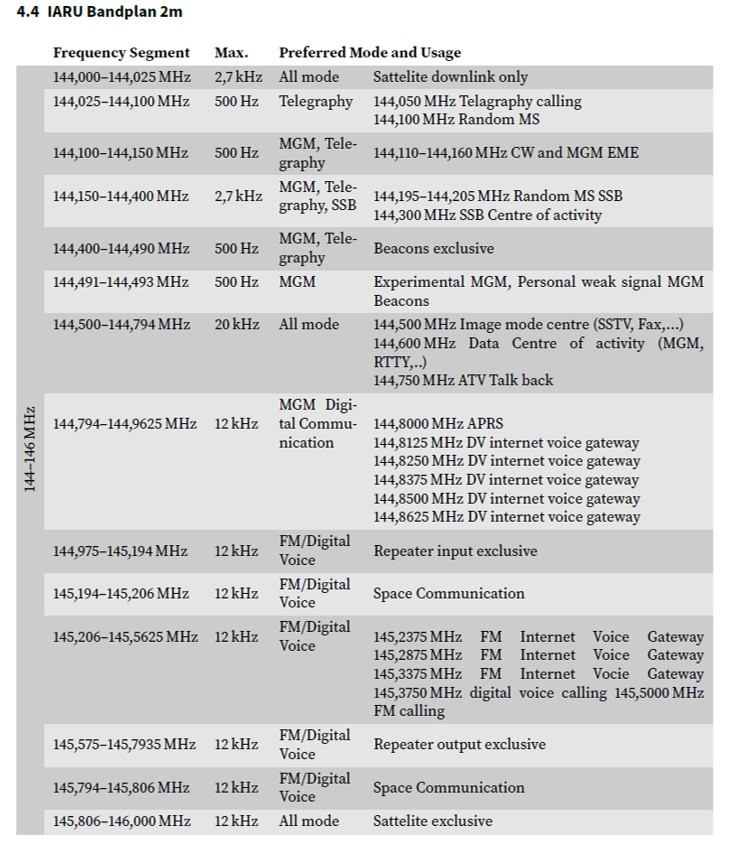
\includegraphics[width=0.85\textwidth]{foto/102}
    \caption{\scriptsize IARU-Bandplan \qty{2}{\metre}}
    \label{n_iaru_bandplan_2m}
\end{figure}

\end{frame}

\begin{frame}
\frametitle{Anruffrequenz}
Um schnell Funkpartner zu finden

\begin{itemize}
  \item FM-Sprechfunk (\enquote{FM calling})
  \item Digitale Telefonie (\enquote{digital voice calling})
  \end{itemize}

\end{frame}

\begin{frame}
\only<1>{
\begin{QQuestion}{BC205}{Welche Frequenz empfiehlt der IARU-Bandplan für einen allgemeinen Anruf mit analoger FM-Telefonie im \qty{2}{m}-Band?}{\qty{145,500}{\MHz}}
{\qty{144,050}{\MHz}}
{\qty{144,800}{\MHz}}
{\qty{145,800}{\MHz}}
\end{QQuestion}

}
\only<2>{
\begin{QQuestion}{BC205}{Welche Frequenz empfiehlt der IARU-Bandplan für einen allgemeinen Anruf mit analoger FM-Telefonie im \qty{2}{m}-Band?}{\textbf{\textcolor{DARCgreen}{\qty{145,500}{\MHz}}}}
{\qty{144,050}{\MHz}}
{\qty{144,800}{\MHz}}
{\qty{145,800}{\MHz}}
\end{QQuestion}

}
\end{frame}

\begin{frame}
\only<1>{
\begin{QQuestion}{BC207}{Welche Frequenz empfiehlt der IARU-Bandplan für einen allgemeinen Anruf mit digitaler Telefonie im \qty{2}{m}-Band?}{\qty{145,500}{\MHz}}
{\qty{145,375}{\MHz}}
{\qty{144,800}{\MHz}}
{\qty{144,195}{\MHz}}
\end{QQuestion}

}
\only<2>{
\begin{QQuestion}{BC207}{Welche Frequenz empfiehlt der IARU-Bandplan für einen allgemeinen Anruf mit digitaler Telefonie im \qty{2}{m}-Band?}{\qty{145,500}{\MHz}}
{\textbf{\textcolor{DARCgreen}{\qty{145,375}{\MHz}}}}
{\qty{144,800}{\MHz}}
{\qty{144,195}{\MHz}}
\end{QQuestion}

}
\end{frame}

\begin{frame}
\frametitle{Frequenzwechsel}
\begin{itemize}
  \item Anruffrequenzen für Anrufe freihalten
  \item Nach Verbindungsaufbau auf eine andere Frequenz verständigen
  \item Nützliche Frequenz aus dem Bandplan entnehmen
  \item Frequenz wechseln
  \end{itemize}
\end{frame}

\begin{frame}
\only<1>{
\begin{QQuestion}{BC209}{Auf welcher der folgenden Frequenzen könnten Sie beispielsweise unter Berücksichtigung des IARU-Bandplans im \qty{2}{\m}-Band eine FM-Telefonieverbindung durchführen?}{\qty{145,450}{\MHz}}
{\qty{144,250}{\MHz}}
{\qty{144,090}{\MHz}}
{\qty{144,450}{\MHz}}
\end{QQuestion}

}
\only<2>{
\begin{QQuestion}{BC209}{Auf welcher der folgenden Frequenzen könnten Sie beispielsweise unter Berücksichtigung des IARU-Bandplans im \qty{2}{\m}-Band eine FM-Telefonieverbindung durchführen?}{\textbf{\textcolor{DARCgreen}{\qty{145,450}{\MHz}}}}
{\qty{144,250}{\MHz}}
{\qty{144,090}{\MHz}}
{\qty{144,450}{\MHz}}
\end{QQuestion}

}
\end{frame}

\begin{frame}
\frametitle{Analoge SSB-Telefonie}
\begin{itemize}
  \item Es gibt keine Anruffrequenz
  \item Stattdessen ein \emph{Aktivitätszentrum} bzw. \emph{center of activity}
  \item Anrufe sollen im Umfeld dieser Frequenz stattfinden
  \item Es kann aber der ganze \enquote{SSB}-Bereich genutzt werden
  \end{itemize}
\end{frame}

\begin{frame}
\only<1>{
\begin{QQuestion}{BC211}{Welche Frequenz bzw. welchen Frequenzbereich sieht der IARU-Bandplan als Aktivitätszentrum für SSB-Telefonie im \qty{2}{m}-Band vor?}{\qty{145,500}{\MHz}}
{\qty{144,300}{\MHz}}
{\qtyrange{144,195}{144,205}{\MHz}}
{\qtyrange{144,110}{144,160}{\MHz}}
\end{QQuestion}

}
\only<2>{
\begin{QQuestion}{BC211}{Welche Frequenz bzw. welchen Frequenzbereich sieht der IARU-Bandplan als Aktivitätszentrum für SSB-Telefonie im \qty{2}{m}-Band vor?}{\qty{145,500}{\MHz}}
{\textbf{\textcolor{DARCgreen}{\qty{144,300}{\MHz}}}}
{\qtyrange{144,195}{144,205}{\MHz}}
{\qtyrange{144,110}{144,160}{\MHz}}
\end{QQuestion}

}
\end{frame}

\begin{frame}
\only<1>{
\begin{QQuestion}{BC210}{Auf welcher der folgenden Frequenzen könnten Sie unter Berücksichtigung des IARU-Bandplans im \qty{2}{m}-Band eine SSB-Telefonieverbindung beispielsweise durchführen?}{\qty{144,800}{\MHz}}
{\qty{145,450}{\MHz}}
{\qty{144,310}{\MHz}}
{\qty{144,450}{\MHz}}
\end{QQuestion}

}
\only<2>{
\begin{QQuestion}{BC210}{Auf welcher der folgenden Frequenzen könnten Sie unter Berücksichtigung des IARU-Bandplans im \qty{2}{m}-Band eine SSB-Telefonieverbindung beispielsweise durchführen?}{\qty{144,800}{\MHz}}
{\qty{145,450}{\MHz}}
{\textbf{\textcolor{DARCgreen}{\qty{144,310}{\MHz}}}}
{\qty{144,450}{\MHz}}
\end{QQuestion}

}
\end{frame}

\begin{frame}
\frametitle{Reservierte Frequenzbereiche}
\begin{itemize}
  \item Satelliten-Up- und Downlink (\enquote{satellite uplink}, \enquote{satellite downlink})
  \item Baken (\enquote{beacons})
  \item Relaisfunkstellen, Eingabe und Ausgabe (\enquote{repeater input}, \enquote{repeater output})
  \item Weltraumkommunikation (\enquote{space communication})
  \item Morsetelegrafie (\enquote{CW})
  \end{itemize}

\end{frame}

\begin{frame}
\only<1>{
\begin{QQuestion}{BC214}{Warum sollten Sie auf \qty{144,125}{\MHz} \underline{keine} Direktverbindung in FM-Telefonie zu einem Funkamateur aufnehmen, der sich im Nachbarort befindet? Der IARU-Bandplan empfiehlt diesen Bereich für die Nutzung durch~...}{Baken.}
{Repeater.}
{Weltraumkommunikation.}
{Morsetelegrafie und schmalbandige digitale Übertragungsverfahren.}
\end{QQuestion}

}
\only<2>{
\begin{QQuestion}{BC214}{Warum sollten Sie auf \qty{144,125}{\MHz} \underline{keine} Direktverbindung in FM-Telefonie zu einem Funkamateur aufnehmen, der sich im Nachbarort befindet? Der IARU-Bandplan empfiehlt diesen Bereich für die Nutzung durch~...}{Baken.}
{Repeater.}
{Weltraumkommunikation.}
{\textbf{\textcolor{DARCgreen}{Morsetelegrafie und schmalbandige digitale Übertragungsverfahren.}}}
\end{QQuestion}

}
\end{frame}

\begin{frame}
\only<1>{
\begin{QQuestion}{BC215}{Warum sollten Sie auf \qty{144,450}{\MHz} \underline{keine} Direktverbindung in FM-Telefonie zu einem Funkamateur aufnehmen, der sich im Nachbarort befindet? Der IARU-Bandplan sieht diesen Bereich exklusiv für die Nutzung durch~...}{Baken vor.}
{Repeater vor.}
{Weltraumkommunikation vor.}
{Morsetelegrafie und schmalbandige digitale Übertragungsverfahren vor.}
\end{QQuestion}

}
\only<2>{
\begin{QQuestion}{BC215}{Warum sollten Sie auf \qty{144,450}{\MHz} \underline{keine} Direktverbindung in FM-Telefonie zu einem Funkamateur aufnehmen, der sich im Nachbarort befindet? Der IARU-Bandplan sieht diesen Bereich exklusiv für die Nutzung durch~...}{\textbf{\textcolor{DARCgreen}{Baken vor.}}}
{Repeater vor.}
{Weltraumkommunikation vor.}
{Morsetelegrafie und schmalbandige digitale Übertragungsverfahren vor.}
\end{QQuestion}

}
\end{frame}

\begin{frame}
\only<1>{
\begin{QQuestion}{BC218}{Warum sollten Sie auf \qty{145,800}{\MHz} \underline{keine} Direktverbindung in FM-Telefonie zu einem Funkamateur aufnehmen, der sich im Nachbarort befindet? Der IARU-Bandplan empfiehlt diesen Bereich für die Nutzung durch ...}{Baken.}
{Repeater.}
{Morsetelegrafie und schmalbandige digitale Übertragungsverfahren.}
{Weltraumkommunikation.}
\end{QQuestion}

}
\only<2>{
\begin{QQuestion}{BC218}{Warum sollten Sie auf \qty{145,800}{\MHz} \underline{keine} Direktverbindung in FM-Telefonie zu einem Funkamateur aufnehmen, der sich im Nachbarort befindet? Der IARU-Bandplan empfiehlt diesen Bereich für die Nutzung durch ...}{Baken.}
{Repeater.}
{Morsetelegrafie und schmalbandige digitale Übertragungsverfahren.}
{\textbf{\textcolor{DARCgreen}{Weltraumkommunikation.}}}
\end{QQuestion}

}
\end{frame}

\begin{frame}
\only<1>{
\begin{QQuestion}{BC217}{Warum sollten Sie auf \qty{145,600}{\MHz} \underline{keine} Direktverbindung in FM-Telefonie zu einem Funkamateur aufnehmen, der sich im Nachbarort befindet? Der IARU-Bandplan empfiehlt diesen Bereich für die Nutzung durch ...}{Weltraumkommunikation.}
{Repeater.}
{Morsetelegrafie und schmalbandige digitale Übertragungsverfahren.}
{Baken.}
\end{QQuestion}

}
\only<2>{
\begin{QQuestion}{BC217}{Warum sollten Sie auf \qty{145,600}{\MHz} \underline{keine} Direktverbindung in FM-Telefonie zu einem Funkamateur aufnehmen, der sich im Nachbarort befindet? Der IARU-Bandplan empfiehlt diesen Bereich für die Nutzung durch ...}{Weltraumkommunikation.}
{\textbf{\textcolor{DARCgreen}{Repeater.}}}
{Morsetelegrafie und schmalbandige digitale Übertragungsverfahren.}
{Baken.}
\end{QQuestion}

}
\end{frame}

\begin{frame}
\only<1>{
\begin{QQuestion}{BC213}{Warum sollten Sie RTTY, PSK31 oder FT8 \underline{nicht} auf \qty{144,075}{MHz}  verwenden? Der IARU-Bandplan empfiehlt~...}{diesen Bereich bevorzugt für Morsetelegrafie zu nutzen.}
{in diesem Bereich maximal \qty{500}{\Hz} Bandbreite zu belegen, damit der Bereich besser genutzt werden kann.}
{den Einsatz von Computern für die Signalerzeugung zu vermeiden.}
{digitale Verfahren oberhalb von \qty{430}{\MHz} durchzuführen, da dort mehr Bandbreite zur Verfügung steht.}
\end{QQuestion}

}
\only<2>{
\begin{QQuestion}{BC213}{Warum sollten Sie RTTY, PSK31 oder FT8 \underline{nicht} auf \qty{144,075}{MHz}  verwenden? Der IARU-Bandplan empfiehlt~...}{\textbf{\textcolor{DARCgreen}{diesen Bereich bevorzugt für Morsetelegrafie zu nutzen.}}}
{in diesem Bereich maximal \qty{500}{\Hz} Bandbreite zu belegen, damit der Bereich besser genutzt werden kann.}
{den Einsatz von Computern für die Signalerzeugung zu vermeiden.}
{digitale Verfahren oberhalb von \qty{430}{\MHz} durchzuführen, da dort mehr Bandbreite zur Verfügung steht.}
\end{QQuestion}

}
\end{frame}%ENDCONTENT


\section{IARU-Bandplan für 70 cm}
\label{section:iaru_bandplan_70cm}
\begin{frame}%STARTCONTENT

\begin{figure}
    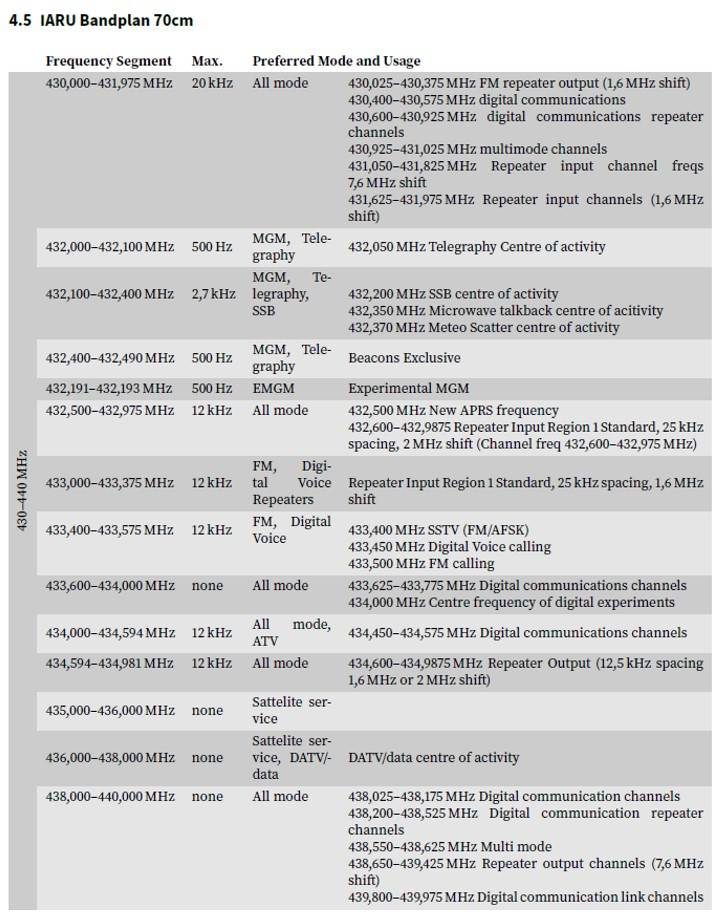
\includegraphics[width=0.85\textwidth]{foto/103}
    \caption{\scriptsize IARU-Bandplan \qty{70}{\centi\metre}}
    \label{n_iaru_bandplan_70cm}
\end{figure}

\end{frame}

\begin{frame}
\only<1>{
\begin{QQuestion}{BC206}{Welche Frequenz empfiehlt der IARU-Bandplan für einen allgemeinen Anruf mit analoger FM-Telefonie im \qty{70}{cm}-Band?}{\qty{433,450}{\MHz}}
{\qty{433,500}{\MHz}}
{\qty{432,500}{\MHz}}
{\qty{432,050}{\MHz}}
\end{QQuestion}

}
\only<2>{
\begin{QQuestion}{BC206}{Welche Frequenz empfiehlt der IARU-Bandplan für einen allgemeinen Anruf mit analoger FM-Telefonie im \qty{70}{cm}-Band?}{\qty{433,450}{\MHz}}
{\textbf{\textcolor{DARCgreen}{\qty{433,500}{\MHz}}}}
{\qty{432,500}{\MHz}}
{\qty{432,050}{\MHz}}
\end{QQuestion}

}
\end{frame}

\begin{frame}
\only<1>{
\begin{QQuestion}{BC208}{Welche Frequenz empfiehlt der IARU-Bandplan für einen allgemeinen Anruf mit digitaler Telefonie im \qty{70}{cm}-Band?}{\qty{433,500}{\MHz}}
{\qty{433,450}{\MHz}}
{\qty{432,500}{\MHz}}
{\qty{432,050}{\MHz}}
\end{QQuestion}

}
\only<2>{
\begin{QQuestion}{BC208}{Welche Frequenz empfiehlt der IARU-Bandplan für einen allgemeinen Anruf mit digitaler Telefonie im \qty{70}{cm}-Band?}{\qty{433,500}{\MHz}}
{\textbf{\textcolor{DARCgreen}{\qty{433,450}{\MHz}}}}
{\qty{432,500}{\MHz}}
{\qty{432,050}{\MHz}}
\end{QQuestion}

}
\end{frame}

\begin{frame}
\only<1>{
\begin{QQuestion}{BC212}{Welche Frequenz bzw. welchen Frequenzbereich sieht der IARU-Bandplan als Aktivitätszentrum für SSB-Telefonie im \qty{70}{cm}-Band vor?}{\qty{434,000}{\MHz}}
{\qty{432,200}{\MHz}}
{\qtyrange{432,600}{432,9875}{\MHz}}
{\qtyrange{434,450}{434,575}{\MHz}}
\end{QQuestion}

}
\only<2>{
\begin{QQuestion}{BC212}{Welche Frequenz bzw. welchen Frequenzbereich sieht der IARU-Bandplan als Aktivitätszentrum für SSB-Telefonie im \qty{70}{cm}-Band vor?}{\qty{434,000}{\MHz}}
{\textbf{\textcolor{DARCgreen}{\qty{432,200}{\MHz}}}}
{\qtyrange{432,600}{432,9875}{\MHz}}
{\qtyrange{434,450}{434,575}{\MHz}}
\end{QQuestion}

}
\end{frame}

\begin{frame}
\only<1>{
\begin{QQuestion}{BC221}{Warum sollten Sie auf \qty{435,500}{\MHz} \underline{keine} Direktverbindung in FM-Telefonie zu einem Funkamateur aufnehmen, der sich im Nachbarort befindet? Der IARU-Bandplan empfiehlt diesen Bereich für die Nutzung durch~...}{Satellitenfunk.}
{Repeater.}
{Morsetelegrafie und schmalbandige digitale Übertragungsverfahren.}
{Baken.}
\end{QQuestion}

}
\only<2>{
\begin{QQuestion}{BC221}{Warum sollten Sie auf \qty{435,500}{\MHz} \underline{keine} Direktverbindung in FM-Telefonie zu einem Funkamateur aufnehmen, der sich im Nachbarort befindet? Der IARU-Bandplan empfiehlt diesen Bereich für die Nutzung durch~...}{\textbf{\textcolor{DARCgreen}{Satellitenfunk.}}}
{Repeater.}
{Morsetelegrafie und schmalbandige digitale Übertragungsverfahren.}
{Baken.}
\end{QQuestion}

}
\end{frame}

\begin{frame}
\only<1>{
\begin{QQuestion}{BC222}{Warum sollten Sie auf \qty{439,200}{\MHz} \underline{keine} Direktverbindung in FM-Telefonie zu einem Funkamateur aufnehmen, der sich im Nachbarort befindet? Der IARU-Bandplan empfiehlt diesen Bereich für die Nutzung durch~...}{Morsetelegrafie und schmalbandige digitale Übertragungsverfahren.}
{Satellitenfunk.}
{Repeater.}
{Baken.}
\end{QQuestion}

}
\only<2>{
\begin{QQuestion}{BC222}{Warum sollten Sie auf \qty{439,200}{\MHz} \underline{keine} Direktverbindung in FM-Telefonie zu einem Funkamateur aufnehmen, der sich im Nachbarort befindet? Der IARU-Bandplan empfiehlt diesen Bereich für die Nutzung durch~...}{Morsetelegrafie und schmalbandige digitale Übertragungsverfahren.}
{Satellitenfunk.}
{\textbf{\textcolor{DARCgreen}{Repeater.}}}
{Baken.}
\end{QQuestion}

}
\end{frame}

\begin{frame}
\only<1>{
\begin{QQuestion}{BC219}{Warum sollten Sie auf \qty{432,040}{\MHz} \underline{keine} Direktverbindung in FM-Telefonie zu einem Funkamateur aufnehmen, der sich im Nachbarort befindet? Der IARU-Bandplan empfiehlt diesen Bereich für die Nutzung durch~...}{Weltraumkommunikation.}
{Satellitenfunk.}
{Morsetelegrafie und schmalbandige digitale Übertragungsverfahren.}
{Baken.}
\end{QQuestion}

}
\only<2>{
\begin{QQuestion}{BC219}{Warum sollten Sie auf \qty{432,040}{\MHz} \underline{keine} Direktverbindung in FM-Telefonie zu einem Funkamateur aufnehmen, der sich im Nachbarort befindet? Der IARU-Bandplan empfiehlt diesen Bereich für die Nutzung durch~...}{Weltraumkommunikation.}
{Satellitenfunk.}
{\textbf{\textcolor{DARCgreen}{Morsetelegrafie und schmalbandige digitale Übertragungsverfahren.}}}
{Baken.}
\end{QQuestion}

}
\end{frame}

\begin{frame}
\only<1>{
\begin{QQuestion}{BC220}{Warum sollten Sie auf \qty{432,450}{\MHz} \underline{keine} Direktverbindung in FM-Telefonie zu einem Funkamateur aufnehmen, der sich im Nachbarort befindet? Der IARU-Bandplan empfiehlt diesen Bereich exklusiv für die Nutzung durch~...}{Satellitenfunk.}
{Baken.}
{Repeater.}
{Morsetelegrafie und schmalbandige digitale Übertragungsverfahren.}
\end{QQuestion}

}
\only<2>{
\begin{QQuestion}{BC220}{Warum sollten Sie auf \qty{432,450}{\MHz} \underline{keine} Direktverbindung in FM-Telefonie zu einem Funkamateur aufnehmen, der sich im Nachbarort befindet? Der IARU-Bandplan empfiehlt diesen Bereich exklusiv für die Nutzung durch~...}{Satellitenfunk.}
{\textbf{\textcolor{DARCgreen}{Baken.}}}
{Repeater.}
{Morsetelegrafie und schmalbandige digitale Übertragungsverfahren.}
\end{QQuestion}

}
\end{frame}%ENDCONTENT


\title{DARC Amateurfunklehrgang Klasse NEA}
\author{Wellenausbreitung}
\institute{Deutscher Amateur Radio Club e.\,V.}
\begin{frame}
\maketitle
\end{frame}

\section{Wellenausbreitung}
\label{section:wellenausbreitung}
\begin{frame}%STARTCONTENT

\begin{columns}
    \begin{column}{0.48\textwidth}
    Je nach Frequenz breitet sich eine Funkwelle anders über unseren Planeten aus.


\begin{figure}
    \DARCimage{0.85\linewidth}{731include}
    \caption{\scriptsize Ionosphäre, Troposhäre und Sporadic-E}
    \label{n_ionosphäre}
\end{figure}


    \end{column}
   \begin{column}{0.48\textwidth}
       \begin{itemize}
  \item Der Funkhorizont, der etwas weiter geht als der sichtbare Horizont (VHF, UHF und höher)
  \item Überreichweiten durch Wetterereignisse in der Troposphäre (VHF, UHF und höher)
  \item Besondere Überreichweiten durch Sporadic-E (VHF, UHF)
  \item Die Raumwelle durch Brechung an der Ionosphäre (Kurzwelle)
  \end{itemize}

   \end{column}
\end{columns}

\end{frame}%ENDCONTENT


\section{Funkhorizont}
\label{section:funkhorizont}
\begin{frame}%STARTCONTENT

\begin{columns}
    \begin{column}{0.48\textwidth}
    
\begin{figure}
    \DARCimage{0.85\linewidth}{484include}
    \caption{\scriptsize Ausbreitung}
    \label{n_funkhorizont}
\end{figure}


    \end{column}
   \begin{column}{0.48\textwidth}
       \begin{itemize}
  \item Funkwellen im VHF- und UHF-Bereich verhalten sich ähnlich wie Licht
  \item Licht reicht maximal bis zum geografischen (sichtbaren) Horizont
  \item Funkwellen schaffen ca. \qty{15}{\percent} mehr Reichweite
  \item Folgen ein wenig der Erdkrümmung
  \end{itemize}

   \end{column}
\end{columns}

\end{frame}

\begin{frame}\begin{itemize}
  \item Sichtverbindung für zuverlässige Funkverbindungen auf VHF, UHF und darüber
  \item Hohe Gebäude oder Berge stören
  \item Je höher die Antenne, umso größer die Reichweite
  \item Weite Verbindungen von Bergen statt aus dem Tal
  \end{itemize}
\end{frame}

\begin{frame}
\only<1>{
\begin{QQuestion}{NH301}{Wie weit etwa reicht der Funkhorizont im UKW-Bereich über den geografischen Horizont hinaus? Er reicht etwa~...}{doppelt so weit.}
{\qty{15}{\percent} weiter.}
{halb so weit.}
{bis zu viermal so weit.}
\end{QQuestion}

}
\only<2>{
\begin{QQuestion}{NH301}{Wie weit etwa reicht der Funkhorizont im UKW-Bereich über den geografischen Horizont hinaus? Er reicht etwa~...}{doppelt so weit.}
{\textbf{\textcolor{DARCgreen}{\qty{15}{\percent} weiter.}}}
{halb so weit.}
{bis zu viermal so weit.}
\end{QQuestion}

}
\end{frame}

\begin{frame}
\only<1>{
\begin{PQuestion}{NH303}{In dem folgenden Geländeprofil sei S ein Sender im \qty{2}{\m}-Band. Welche der Empfangsstationen E1 bis E4 wird das Signal des Senders wahrscheinlich am besten empfangen?}{$\text{E}_3$}
{$\text{E}_1$}
{$\text{E}_2$}
{$\text{E}_4$}
{\DARCimage{1.0\linewidth}{483include}}\end{PQuestion}

}
\only<2>{
\begin{PQuestion}{NH303}{In dem folgenden Geländeprofil sei S ein Sender im \qty{2}{\m}-Band. Welche der Empfangsstationen E1 bis E4 wird das Signal des Senders wahrscheinlich am besten empfangen?}{\textbf{\textcolor{DARCgreen}{$\text{E}_3$}}}
{$\text{E}_1$}
{$\text{E}_2$}
{$\text{E}_4$}
{\DARCimage{1.0\linewidth}{483include}}\end{PQuestion}

}
\end{frame}

\begin{frame}
\only<1>{
\begin{QQuestion}{NH302}{Wie wirkt sich die Antennenhöhe auf die Reichweite einer UKW-Verbindung aus? Die Reichweite steigt mit zunehmender Antennenhöhe, weil~...}{die quasi-optische Sichtweite zunimmt.}
{sie näher an der Ionosphäre ist.}
{dadurch steiler abgestrahlt werden kann.}
{in höheren Luftschichten die Temperatur sinkt.}
\end{QQuestion}

}
\only<2>{
\begin{QQuestion}{NH302}{Wie wirkt sich die Antennenhöhe auf die Reichweite einer UKW-Verbindung aus? Die Reichweite steigt mit zunehmender Antennenhöhe, weil~...}{\textbf{\textcolor{DARCgreen}{die quasi-optische Sichtweite zunimmt.}}}
{sie näher an der Ionosphäre ist.}
{dadurch steiler abgestrahlt werden kann.}
{in höheren Luftschichten die Temperatur sinkt.}
\end{QQuestion}

}
\end{frame}%ENDCONTENT


\section{Troposphärische Inversionsbildung}
\label{section:troposphaere}
\begin{frame}%STARTCONTENT

\begin{columns}
    \begin{column}{0.48\textwidth}
    
\begin{figure}
    \DARCimage{0.85\linewidth}{734include}
    \caption{\scriptsize Troposhärische Inversionsbildung, Schichten unterschiedlicher Temperatur liegen aufeinander, an der Grenze der Schichten werden Funkwellen im VHF-Bereich reflektiert}
    \label{n_tropo}
\end{figure}


    \end{column}
   \begin{column}{0.48\textwidth}
       \begin{itemize}
  \item Besonderer Effekt in der Troposphäre (ca. 15km)
  \item \emph{Troposphärische Inversionsschichten} zwischen warmen und kalten Luftschichten
  \item Führt zu erheblich größeren Reichweiten im VHF-Bereich (800-1000km)
  \item Tritt hauptsächlich im Frühjahr und Herbst auf
  \end{itemize}

   \end{column}
\end{columns}

\end{frame}

\begin{frame}
\only<1>{
\begin{QQuestion}{NH304}{Welcher Effekt ist normalerweise für die Ausbreitung eines VHF-Signals über 800~bis \qty{1 000}{\km} verantwortlich?}{Atmosphärische Absorption}
{Reflexion an der Mondoberfläche}
{Bodenwellenausbreitung}
{Troposphärische Inversionsbildung}
\end{QQuestion}

}
\only<2>{
\begin{QQuestion}{NH304}{Welcher Effekt ist normalerweise für die Ausbreitung eines VHF-Signals über 800~bis \qty{1 000}{\km} verantwortlich?}{Atmosphärische Absorption}
{Reflexion an der Mondoberfläche}
{Bodenwellenausbreitung}
{\textbf{\textcolor{DARCgreen}{Troposphärische Inversionsbildung}}}
\end{QQuestion}

}
\end{frame}%ENDCONTENT


\section{Troposphäre II}
\label{section:troposphaere_2}
\begin{frame}%STARTCONTENT

\frametitle{Begriffe}
Im folgenden Kapitel werden mehrere Begriffe verwendet, die vorab erklärt werden

\begin{itemize}
  \item \emph{Beugung}: Wellen werden an einem Hindernis abgelenkt
  \item \emph{Streuung}: Ablenkung der Wellen durch Interaktion von Teilchen
  \item \emph{Reflexion}: Gleichgerichtete Streuung
  \item \emph{Brechung} oder \emph{Refraktion}: Ablenkung der Wellen durch Änderung der Ausbreitungsgeschwindigkeit durch ein anderes Medium mit anderer Dichte
  \end{itemize}
\end{frame}

\begin{frame}
\begin{columns}
    \begin{column}{0.48\textwidth}
    \begin{itemize}
  \item Bereits bekannt: Die für den Amateurfunk relevanten Schichten in der Atmosphäre
  \item In der Troposphäre finden Erscheinungen des Wetters statt
  \end{itemize}

    \end{column}
   \begin{column}{0.48\textwidth}
       
\begin{figure}
    \DARCimage{0.85\linewidth}{731include}
    \caption{\scriptsize Für den Amateurfunk relevante Schichten in der Atmosphäre}
    \label{e_atmosphaeren_schichten}
\end{figure}


   \end{column}
\end{columns}

\end{frame}

\begin{frame}
\frametitle{DX in VHF/UHF}
\begin{columns}
    \begin{column}{0.48\textwidth}
    \begin{itemize}
  \item Überhorizontverbindungen bei VHF/UHF entstehen durch Beugung, Reflexion und Streuung in der Troposphäre
  \item Bereiche mit unterschiedlicher Temperatur und Dichte
  \end{itemize}

    \end{column}
   \begin{column}{0.48\textwidth}
       
\begin{figure}
    \DARCimage{0.85\linewidth}{734include}
    \caption{\scriptsize Troposphärische Ausbreitung an verschiedenen Luftschichten}
    \label{e_tropo}
\end{figure}


   \end{column}
\end{columns}

\end{frame}

\begin{frame}
\only<1>{
\begin{QQuestion}{EH301}{Was ist die \glqq Troposphäre\grqq{}? Die Troposphäre ist der Teil der Atmosphäre,~...}{in welchem Aurora-Erscheinungen auftreten können.}
{der sich über den Tropen befindet.}
{in dem es zur Bildung sporadischer E-Regionen kommen kann.}
{in der die Erscheinungen des Wetters stattfinden.}
\end{QQuestion}

}
\only<2>{
\begin{QQuestion}{EH301}{Was ist die \glqq Troposphäre\grqq{}? Die Troposphäre ist der Teil der Atmosphäre,~...}{in welchem Aurora-Erscheinungen auftreten können.}
{der sich über den Tropen befindet.}
{in dem es zur Bildung sporadischer E-Regionen kommen kann.}
{\textbf{\textcolor{DARCgreen}{in der die Erscheinungen des Wetters stattfinden.}}}
\end{QQuestion}

}
\end{frame}

\begin{frame}
\only<1>{
\begin{QQuestion}{EH302}{Überhorizontverbindungen im VHF/UHF-Bereich kommen u.~a. zustande durch~...}{Polarisationsdrehungen in der Troposphäre bei hoch liegender Bewölkung.}
{Beugung, Reflexion und Streuung der Wellen in der Troposphäre durch das Auftreten sporadischer D-Regionen.}
{Beugung, Reflexion und Streuung der Wellen an troposphärischen Bereichen unterschiedlicher Temperatur und Dichte.}
{Polarisationsdrehungen in der Troposphäre an Gewitterfronten.}
\end{QQuestion}

}
\only<2>{
\begin{QQuestion}{EH302}{Überhorizontverbindungen im VHF/UHF-Bereich kommen u.~a. zustande durch~...}{Polarisationsdrehungen in der Troposphäre bei hoch liegender Bewölkung.}
{Beugung, Reflexion und Streuung der Wellen in der Troposphäre durch das Auftreten sporadischer D-Regionen.}
{\textbf{\textcolor{DARCgreen}{Beugung, Reflexion und Streuung der Wellen an troposphärischen Bereichen unterschiedlicher Temperatur und Dichte.}}}
{Polarisationsdrehungen in der Troposphäre an Gewitterfronten.}
\end{QQuestion}

}
\end{frame}

\begin{frame}
\only<1>{
\begin{QQuestion}{EH303}{Für VHF-Weitverkehrsverbindungen wird hauptsächlich die~...}{ionosphärische Ausbreitung genutzt.}
{troposphärische Ausbreitung genutzt.}
{Bodenwellenausbreitung genutzt.}
{Oberflächenwellenausbreitung genutzt.}
\end{QQuestion}

}
\only<2>{
\begin{QQuestion}{EH303}{Für VHF-Weitverkehrsverbindungen wird hauptsächlich die~...}{ionosphärische Ausbreitung genutzt.}
{\textbf{\textcolor{DARCgreen}{troposphärische Ausbreitung genutzt.}}}
{Bodenwellenausbreitung genutzt.}
{Oberflächenwellenausbreitung genutzt.}
\end{QQuestion}

}
\end{frame}%ENDCONTENT


\section{Troposphäre III}
\label{section:troposphaere_3}
\begin{frame}%STARTCONTENT

\frametitle{Foliensatz in Arbeit}
2024-04-28: Die Inhalte werden noch aufbereitet.

Derzeit sind in diesem Abschnitt nur die Fragen sortiert enthalten.

Für das Selbststudium verweisen wir aktuell auf den Abschnitt Wellenausbreitung im DARC Online Lehrgang (\textcolor{DARCblue}{\faLink~\href{https://www.darc.de/der-club/referate/ajw/lehrgang-te/e09/}{www.darc.de/der-club/referate/ajw/lehrgang-te/e09/}}) für die Prüfung bis Juni 2024. Bis auf die Fragen hat sich an der Thematik nichts geändert. Das Thema war bisher Stoff der Klasse~E und wurde mit der neuen Prüfungsordnung auf alle drei Klassen aufgeteilt.

\end{frame}

\begin{frame}
\frametitle{Lage der Ionosphären-Schichten}

\begin{figure}
    \DARCimage{0.85\linewidth}{731include}
    \caption{\scriptsize Für den Amateurfunk relevante Schichten in der Atmosphäre}
    \label{e_atmosphaeren_schichten}
\end{figure}

\end{frame}

\begin{frame}
\only<1>{
\begin{QQuestion}{AH105}{In welcher Höhe befindet sich die für die Fernausbreitung (DX) wichtige F1-Region während der Tagesstunden? Sie befindet sich in ungefähr~...}{\qtyrange{200}{450}{\km} Höhe.}
{\qtyrange{90}{130}{\km} Höhe.}
{\qtyrange{50}{90}{\km} Höhe.}
{\qtyrange{130}{200}{\km} Höhe.}
\end{QQuestion}

}
\only<2>{
\begin{QQuestion}{AH105}{In welcher Höhe befindet sich die für die Fernausbreitung (DX) wichtige F1-Region während der Tagesstunden? Sie befindet sich in ungefähr~...}{\qtyrange{200}{450}{\km} Höhe.}
{\qtyrange{90}{130}{\km} Höhe.}
{\qtyrange{50}{90}{\km} Höhe.}
{\textbf{\textcolor{DARCgreen}{\qtyrange{130}{200}{\km} Höhe.}}}
\end{QQuestion}

}
\end{frame}

\begin{frame}
\only<1>{
\begin{QQuestion}{AH106}{In welcher Höhe befindet sich die für die Fernausbreitung (DX) wichtige F2-Region während der Tagesstunden an einem Sommertag? Sie befindet sich in ungefähr~...}{\qtyrange{130}{200}{\km} Höhe.}
{\qtyrange{250}{450}{\km} Höhe.}
{\qtyrange{90}{130}{\km} Höhe.}
{\qtyrange{50}{90}{\km} Höhe.}
\end{QQuestion}

}
\only<2>{
\begin{QQuestion}{AH106}{In welcher Höhe befindet sich die für die Fernausbreitung (DX) wichtige F2-Region während der Tagesstunden an einem Sommertag? Sie befindet sich in ungefähr~...}{\qtyrange{130}{200}{\km} Höhe.}
{\textbf{\textcolor{DARCgreen}{\qtyrange{250}{450}{\km} Höhe.}}}
{\qtyrange{90}{130}{\km} Höhe.}
{\qtyrange{50}{90}{\km} Höhe.}
\end{QQuestion}

}
\end{frame}

\begin{frame}
\frametitle{Effekte der Ionisierung}
\end{frame}

\begin{frame}
\only<1>{
\begin{QQuestion}{AH101}{Welcher Effekt sorgt hauptsächlich dafür, dass ionosphärische Regionen Funkwellen zur Erde ablenken können?}{Die von der Sonne ausgehende Infrarotstrahlung ionisiert~-~je nach Strahlungsintensität~-~die Moleküle in den verschiedenen Regionen.}
{Die von der Sonne ausgehende UV-Strahlung ionisiert~-~je nach Strahlungsintensität~-~die Moleküle in den verschiedenen Regionen.}
{Die von der Sonne ausgehende UV-Strahlung aktiviert~-~je nach Strahlungsintensität~-~die Sauerstoffatome in den verschiedenen Regionen.}
{Die von der Sonne ausgehende Infrarotstrahlung aktiviert~-~je nach Strahlungsintensität~-~die Sauerstoffatome in den verschiedenen Regionen.}
\end{QQuestion}

}
\only<2>{
\begin{QQuestion}{AH101}{Welcher Effekt sorgt hauptsächlich dafür, dass ionosphärische Regionen Funkwellen zur Erde ablenken können?}{Die von der Sonne ausgehende Infrarotstrahlung ionisiert~-~je nach Strahlungsintensität~-~die Moleküle in den verschiedenen Regionen.}
{\textbf{\textcolor{DARCgreen}{Die von der Sonne ausgehende UV-Strahlung ionisiert~-~je nach Strahlungsintensität~-~die Moleküle in den verschiedenen Regionen.}}}
{Die von der Sonne ausgehende UV-Strahlung aktiviert~-~je nach Strahlungsintensität~-~die Sauerstoffatome in den verschiedenen Regionen.}
{Die von der Sonne ausgehende Infrarotstrahlung aktiviert~-~je nach Strahlungsintensität~-~die Sauerstoffatome in den verschiedenen Regionen.}
\end{QQuestion}

}
\end{frame}

\begin{frame}
\only<1>{
\begin{QQuestion}{AH108}{Zu welcher Jahres- und Tageszeit hat die F2-Region ihre größte Höhe? Sie hat ihre größte Höhe~...}{im Sommer um Mitternacht.}
{im Sommer zur Mittagszeit.}
{im Frühjahr und Herbst zur Dämmerungszeit.}
{im Winter zur Mittagszeit.}
\end{QQuestion}

}
\only<2>{
\begin{QQuestion}{AH108}{Zu welcher Jahres- und Tageszeit hat die F2-Region ihre größte Höhe? Sie hat ihre größte Höhe~...}{im Sommer um Mitternacht.}
{\textbf{\textcolor{DARCgreen}{im Sommer zur Mittagszeit.}}}
{im Frühjahr und Herbst zur Dämmerungszeit.}
{im Winter zur Mittagszeit.}
\end{QQuestion}

}
\end{frame}

\begin{frame}
\only<1>{
\begin{QQuestion}{AH221}{Massiv erhöhte UV- und Röntgenstrahlung, wie sie vor allem durch starke Sonneneruptionen hervorgerufen wird, beeinflusst in der Ionosphäre vor allem~...}{die F2-Region, die dann so stark ionisiert wird, dass fast die gesamte KW-Ausstrahlung reflektiert wird.}
{die D-Region, die die Kurzwellen-Signale dann so massiv dämpft, dass keine Ausbreitung über die Raumwelle mehr möglich ist.}
{die E-Region, die dann für die höheren Frequenzen durchlässiger wird und durch Refraktion (Brechung) in der F2-Region für gute Ausbreitungsbedingungen sorgt.}
{die F1-Region, die durch Absorption der höheren Frequenzen die Refraktion (Brechung) an der F2-Region behindert.}
\end{QQuestion}

}
\only<2>{
\begin{QQuestion}{AH221}{Massiv erhöhte UV- und Röntgenstrahlung, wie sie vor allem durch starke Sonneneruptionen hervorgerufen wird, beeinflusst in der Ionosphäre vor allem~...}{die F2-Region, die dann so stark ionisiert wird, dass fast die gesamte KW-Ausstrahlung reflektiert wird.}
{\textbf{\textcolor{DARCgreen}{die D-Region, die die Kurzwellen-Signale dann so massiv dämpft, dass keine Ausbreitung über die Raumwelle mehr möglich ist.}}}
{die E-Region, die dann für die höheren Frequenzen durchlässiger wird und durch Refraktion (Brechung) in der F2-Region für gute Ausbreitungsbedingungen sorgt.}
{die F1-Region, die durch Absorption der höheren Frequenzen die Refraktion (Brechung) an der F2-Region behindert.}
\end{QQuestion}

}
\end{frame}

\begin{frame}
\frametitle{Polarisation}
\end{frame}

\begin{frame}
\only<1>{
\begin{QQuestion}{AH219}{Wie wird die Polarisation einer elektromagnetischen Welle bei der Ausbreitung über die Raumwelle beeinflusst?}{Die Polarisation der ausgesendeten Wellen wird in der Ionosphäre stets um \qty{90}{\degree} gedreht.}
{Die Polarisation der ausgesendeten Wellen bleibt bei der Refraktion (Brechung) in der Ionosphäre stets unverändert.}
{Die Polarisation der ausgesendeten Wellen wird bei der Refraktion (Brechung) in der Ionosphäre stets verändert.}
{Die Polarisation der ausgesendeten Wellen wird bei jedem Sprung (Hop) in der Ionosphäre um \qty{90}{\degree} gedreht.}
\end{QQuestion}

}
\only<2>{
\begin{QQuestion}{AH219}{Wie wird die Polarisation einer elektromagnetischen Welle bei der Ausbreitung über die Raumwelle beeinflusst?}{Die Polarisation der ausgesendeten Wellen wird in der Ionosphäre stets um \qty{90}{\degree} gedreht.}
{Die Polarisation der ausgesendeten Wellen bleibt bei der Refraktion (Brechung) in der Ionosphäre stets unverändert.}
{\textbf{\textcolor{DARCgreen}{Die Polarisation der ausgesendeten Wellen wird bei der Refraktion (Brechung) in der Ionosphäre stets verändert.}}}
{Die Polarisation der ausgesendeten Wellen wird bei jedem Sprung (Hop) in der Ionosphäre um \qty{90}{\degree} gedreht.}
\end{QQuestion}

}
\end{frame}

\begin{frame}
\frametitle{Funkwellen-Ausbreitung}
\end{frame}

\begin{frame}
\only<1>{
\begin{QQuestion}{AH201}{Welches der nachstehend aufgeführten Bänder ist für KW-Verbindungen zwischen Hamburg und München um die Mittagszeit herum üblicherweise gut geeignet?}{\qty{40}{\m}-Band}
{\qty{160}{\m}-Band}
{\qty{80}{\m}-Band}
{\qty{15}{\m}-Band}
\end{QQuestion}

}
\only<2>{
\begin{QQuestion}{AH201}{Welches der nachstehend aufgeführten Bänder ist für KW-Verbindungen zwischen Hamburg und München um die Mittagszeit herum üblicherweise gut geeignet?}{\textbf{\textcolor{DARCgreen}{\qty{40}{\m}-Band}}}
{\qty{160}{\m}-Band}
{\qty{80}{\m}-Band}
{\qty{15}{\m}-Band}
\end{QQuestion}

}
\end{frame}

\begin{frame}
\only<1>{
\begin{QQuestion}{AH203}{Welche der folgenden Frequenzbänder können in den Nachtstunden am ehesten für weltweite Funkverbindungen genutzt werden?}{\qty{160}{\m}, \qty{80}{\m} und \qty{40}{\m}}
{\qty{40}{\m}, \qty{20}{\m} und \qty{15}{\m}}
{\qty{40}{\m}, \qty{17}{\m} und \qty{6}{\m}}
{ \qty{30}{\m}, \qty{12}{\m} und \qty{10}{\m}}
\end{QQuestion}

}
\only<2>{
\begin{QQuestion}{AH203}{Welche der folgenden Frequenzbänder können in den Nachtstunden am ehesten für weltweite Funkverbindungen genutzt werden?}{\textbf{\textcolor{DARCgreen}{\qty{160}{\m}, \qty{80}{\m} und \qty{40}{\m}}}}
{\qty{40}{\m}, \qty{20}{\m} und \qty{15}{\m}}
{\qty{40}{\m}, \qty{17}{\m} und \qty{6}{\m}}
{ \qty{30}{\m}, \qty{12}{\m} und \qty{10}{\m}}
\end{QQuestion}

}
\end{frame}

\begin{frame}
\only<1>{
\begin{QQuestion}{AH107}{Für die DX-Kurzwellenausbreitung über die Raumwelle ist die F1-Region~...}{erwünscht, weil sie durch zusätzliche Reflexion die Wirkung der F2-Region verstärken kann.}
{meist unerwünscht, weil sie durch Abdeckung die Ausbreitung durch Refraktion (Brechung) an der F2-Region verhindern kann.}
{nicht von großer Bedeutung, weil sie vor allem für die höheren Frequenzen durchlässig ist.}
{von großer Bedeutung, weil sie die Dämpfung in der E-Region senkt und damit die Sprungdistanz vergrößert.}
\end{QQuestion}

}
\only<2>{
\begin{QQuestion}{AH107}{Für die DX-Kurzwellenausbreitung über die Raumwelle ist die F1-Region~...}{erwünscht, weil sie durch zusätzliche Reflexion die Wirkung der F2-Region verstärken kann.}
{\textbf{\textcolor{DARCgreen}{meist unerwünscht, weil sie durch Abdeckung die Ausbreitung durch Refraktion (Brechung) an der F2-Region verhindern kann.}}}
{nicht von großer Bedeutung, weil sie vor allem für die höheren Frequenzen durchlässig ist.}
{von großer Bedeutung, weil sie die Dämpfung in der E-Region senkt und damit die Sprungdistanz vergrößert.}
\end{QQuestion}

}
\end{frame}

\begin{frame}
\frametitle{Troposphärische Ausbreitung}
\end{frame}

\begin{frame}
\only<1>{
\begin{QQuestion}{AH309}{Überhorizontverbindungen im VHF/UHF-Bereich kommen unter anderem zustande durch~...}{Polarisationsdrehungen in der Troposphäre an Gewitterfronten.}
{Reflexion der Wellen in der Troposphäre durch das Auftreten sporadischer D-Regionen.}
{Polarisationsdrehungen in der Troposphäre bei hoch liegender Bewölkung.}
{troposphärische Duct-Übertragung beim Auftreten von Inversionsschichten.}
\end{QQuestion}

}
\only<2>{
\begin{QQuestion}{AH309}{Überhorizontverbindungen im VHF/UHF-Bereich kommen unter anderem zustande durch~...}{Polarisationsdrehungen in der Troposphäre an Gewitterfronten.}
{Reflexion der Wellen in der Troposphäre durch das Auftreten sporadischer D-Regionen.}
{Polarisationsdrehungen in der Troposphäre bei hoch liegender Bewölkung.}
{\textbf{\textcolor{DARCgreen}{troposphärische Duct-Übertragung beim Auftreten von Inversionsschichten.}}}
\end{QQuestion}

}
\end{frame}%ENDCONTENT


\section{Mehrwegeausbreitung}
\label{section:mehrwegeausbreitung}
\begin{frame}%STARTCONTENT

\begin{columns}
    \begin{column}{0.48\textwidth}
    \begin{itemize}
  \item Funksignal gelangt auf mehr als einem Weg vom Sender zum Empfänger
  \item Reflexion an Gebäude, Gelände, Flugzeuge etc.
  \item Refraktion an Ionossphäre bei Kurzwelle
  \item Führt zu Interferenz mit Verstärkung oder Auslöschung des Signals
  \end{itemize}

    \end{column}
   \begin{column}{0.48\textwidth}
       
   \end{column}
\end{columns}

\end{frame}

\begin{frame}\end{frame}%ENDCONTENT


\section{Aurora I}
\label{section:aurora_1}
\begin{frame}%STARTCONTENT

\begin{figure}
    \includegraphics[width=0.85\textwidth]{foto/217}
    \caption{\scriptsize Aurora am Notfunk Ausbildungswochenende im Mai 2024}
    \label{e_aurora}
\end{figure}
\end{frame}

\begin{frame}\begin{itemize}
  \item Aurora- oder Polarlichterscheinung in ca. \qtyrange{90}{200}{\kilo\metre} Höhe
  \item Hauptsächlich über magnetischen Nord- und Südpol
  \item Sauerstoff- und Stickstoffatome werden vom Sonnenwind angeregt oder ionisiert
  \item Sonnenwind: Elektrisch geladene Teilchen
  \item Bei Sonneneruptionen besonders stark
  \end{itemize}
\end{frame}

\begin{frame}
\frametitle{Aurora und Amateurfunk}
\begin{itemize}
  \item Funkwellen können sich an ionisierten Sauerstoff- und Stickstoffatomen brechen
  \item Insbesondere für VHF-DX-Verbindungen nutzbar
  \item Sprache nur schlecht nutzbar (große Bandbreite)
  \item Für CW und Digimodes brauchbar
  \item Rapport: für T wird \enquote{A} vergeben, da Ton rau und schwankend ist 
  \end{itemize}
\end{frame}

\begin{frame}
\only<1>{
\begin{QQuestion}{EH305}{Wie wird ein Aurora-Signal in Morsetelegrafie beurteilt?}{Es wird beurteilt mit R und T, weil die Signalstärke stark schwankt.}
{Es wird beurteilt mit R, S und T, da Aurora-Verbindungen überwiegend in CW getätigt werden.}
{Es wird beurteilt mit R, S und \glqq A\grqq{} für Aurora, da der Ton bei Aurora sehr rau ist und nicht beurteilt werden kann.}
{Es wird beurteilt mit R, S, T und \glqq A\grqq{} für Aurora.}
\end{QQuestion}

}
\only<2>{
\begin{QQuestion}{EH305}{Wie wird ein Aurora-Signal in Morsetelegrafie beurteilt?}{Es wird beurteilt mit R und T, weil die Signalstärke stark schwankt.}
{Es wird beurteilt mit R, S und T, da Aurora-Verbindungen überwiegend in CW getätigt werden.}
{\textbf{\textcolor{DARCgreen}{Es wird beurteilt mit R, S und \glqq A\grqq{} für Aurora, da der Ton bei Aurora sehr rau ist und nicht beurteilt werden kann.}}}
{Es wird beurteilt mit R, S, T und \glqq A\grqq{} für Aurora.}
\end{QQuestion}

}
\end{frame}%ENDCONTENT


\section{Aurora II}
\label{section:aurora_2}
\begin{frame}%STARTCONTENT

\frametitle{Foliensatz in Arbeit}
2024-04-28: Die Inhalte werden noch aufbereitet.

Derzeit sind in diesem Abschnitt nur die Fragen sortiert enthalten.

Für das Selbststudium verweisen wir aktuell auf den Abschnitt Wellenausbreitung im DARC Online Lehrgang (\textcolor{DARCblue}{\faLink~\href{https://www.darc.de/der-club/referate/ajw/lehrgang-te/e09/}{www.darc.de/der-club/referate/ajw/lehrgang-te/e09/}}) für die Prüfung bis Juni 2024. Bis auf die Fragen hat sich an der Thematik nichts geändert. Das Thema war bisher Stoff der Klasse~E und wurde mit der neuen Prüfungsordnung auf alle drei Klassen aufgeteilt.

\end{frame}

\begin{frame}
\frametitle{Auftreten von Aurora}

\end{frame}

\begin{frame}
\only<1>{
\begin{QQuestion}{AH302}{In welchem ionosphärischen Bereich treten gelegentlich Aurora-Erscheinungen auf?}{In der E-Region in der Nähe der Pole}
{In der F-Region}
{In der E-Region in der Nähe des Äquators.}
{In der D-Region}
\end{QQuestion}

}
\only<2>{
\begin{QQuestion}{AH302}{In welchem ionosphärischen Bereich treten gelegentlich Aurora-Erscheinungen auf?}{\textbf{\textcolor{DARCgreen}{In der E-Region in der Nähe der Pole}}}
{In der F-Region}
{In der E-Region in der Nähe des Äquators.}
{In der D-Region}
\end{QQuestion}

}
\end{frame}

\begin{frame}
\only<1>{
\begin{QQuestion}{AH303}{Was ist die Ursache für Aurora-Erscheinungen?}{Das Eindringen geladener Teilchen von der Sonne in die Atmosphäre der Polarregionen.}
{Eine hohe Sonnenfleckenzahl.}
{Eine niedrige Sonnenfleckenzahl.}
{Das Eindringen starker Meteoritenschauer in die Atmosphäre der Polarregionen.}
\end{QQuestion}

}
\only<2>{
\begin{QQuestion}{AH303}{Was ist die Ursache für Aurora-Erscheinungen?}{\textbf{\textcolor{DARCgreen}{Das Eindringen geladener Teilchen von der Sonne in die Atmosphäre der Polarregionen.}}}
{Eine hohe Sonnenfleckenzahl.}
{Eine niedrige Sonnenfleckenzahl.}
{Das Eindringen starker Meteoritenschauer in die Atmosphäre der Polarregionen.}
\end{QQuestion}

}
\end{frame}

\begin{frame}
\only<1>{
\begin{QQuestion}{AH306}{In welche Himmelsrichtung muss eine Funkstation in Europa ihre VHF-Antenne drehen, um eine Verbindung über \glqq Aurora\grqq{} abzuwickeln?}{Süden}
{Norden}
{Osten}
{Westen}
\end{QQuestion}

}
\only<2>{
\begin{QQuestion}{AH306}{In welche Himmelsrichtung muss eine Funkstation in Europa ihre VHF-Antenne drehen, um eine Verbindung über \glqq Aurora\grqq{} abzuwickeln?}{Süden}
{\textbf{\textcolor{DARCgreen}{Norden}}}
{Osten}
{Westen}
\end{QQuestion}

}
\end{frame}

\begin{frame}
\frametitle{Nutzung für Wellenausbreitung}
\end{frame}

\begin{frame}
\only<1>{
\begin{QQuestion}{AH304}{Beim Auftreten von Polarlichtern lassen sich auf den Amateurfunkbändern über \qty{30}{\MHz} beträchtliche Überreichweiten erzielen, weil~...}{stark ionisierte Bereiche auftreten, die Funkwellen reflektieren.}
{starke Magnetfelder auftreten, die Funkwellen reflektieren.}
{starke Inversionsfelder auftreten, die Funkwellen reflektieren.}
{starke sporadische D-Regionen auftreten, die Funkwellen reflektieren.}
\end{QQuestion}

}
\only<2>{
\begin{QQuestion}{AH304}{Beim Auftreten von Polarlichtern lassen sich auf den Amateurfunkbändern über \qty{30}{\MHz} beträchtliche Überreichweiten erzielen, weil~...}{\textbf{\textcolor{DARCgreen}{stark ionisierte Bereiche auftreten, die Funkwellen reflektieren.}}}
{starke Magnetfelder auftreten, die Funkwellen reflektieren.}
{starke Inversionsfelder auftreten, die Funkwellen reflektieren.}
{starke sporadische D-Regionen auftreten, die Funkwellen reflektieren.}
\end{QQuestion}

}
\end{frame}

\begin{frame}
\only<1>{
\begin{QQuestion}{AH305}{Was meint ein Funkamateur damit, wenn er angibt, dass er auf dem \qty{2}{\m}-Band eine Aurora-Verbindung mit Schottland gehabt hat?}{Die Verbindung ist durch Verstärkung der polaren Nordlichter mittels Ultrakurzwellen zustande gekommen (Reflexion von ionisiertem Polarlicht).}
{Die Verbindung ist durch Beugung von Ultrakurzwellen an Lichtquellen der Polarregion zustande gekommen (Beugung an ionisierten Polarschichten).}
{Die Verbindung ist durch Reflexion von Ultrakurzwellen an polaren Nordlichtern zustande gekommen (Reflexion an polaren Ionisationserscheinungen).}
{Die Verbindung ist durch Reflexion von verbrummten Ultrakurzwellen am Polarkreis zustande gekommen (Reflexion an Ionisationserscheinungen des Polarkreises).}
\end{QQuestion}

}
\only<2>{
\begin{QQuestion}{AH305}{Was meint ein Funkamateur damit, wenn er angibt, dass er auf dem \qty{2}{\m}-Band eine Aurora-Verbindung mit Schottland gehabt hat?}{Die Verbindung ist durch Verstärkung der polaren Nordlichter mittels Ultrakurzwellen zustande gekommen (Reflexion von ionisiertem Polarlicht).}
{Die Verbindung ist durch Beugung von Ultrakurzwellen an Lichtquellen der Polarregion zustande gekommen (Beugung an ionisierten Polarschichten).}
{\textbf{\textcolor{DARCgreen}{Die Verbindung ist durch Reflexion von Ultrakurzwellen an polaren Nordlichtern zustande gekommen (Reflexion an polaren Ionisationserscheinungen).}}}
{Die Verbindung ist durch Reflexion von verbrummten Ultrakurzwellen am Polarkreis zustande gekommen (Reflexion an Ionisationserscheinungen des Polarkreises).}
\end{QQuestion}

}
\end{frame}

\begin{frame}
\only<1>{
\begin{QQuestion}{AH307}{Welches der folgenden Übertragungsverfahren eignet sich am besten für Auroraverbindungen?}{SSB}
{CW}
{FM}
{RTTY}
\end{QQuestion}

}
\only<2>{
\begin{QQuestion}{AH307}{Welches der folgenden Übertragungsverfahren eignet sich am besten für Auroraverbindungen?}{SSB}
{\textbf{\textcolor{DARCgreen}{CW}}}
{FM}
{RTTY}
\end{QQuestion}

}
\end{frame}

\begin{frame}
\only<1>{
\begin{QQuestion}{AH308}{Wie wirkt sich \glqq Aurora\grqq{} auf die Signalqualität eines Funksignals aus?}{CW-Signale haben einen flatternden und verbrummten Ton.}
{CW-Signale haben einen besseren Ton.}
{Die Lesbarkeit von Fonie-Signalen verbessert sich.}
{CW- und Fonie-Signale haben ein Echo.}
\end{QQuestion}

}
\only<2>{
\begin{QQuestion}{AH308}{Wie wirkt sich \glqq Aurora\grqq{} auf die Signalqualität eines Funksignals aus?}{\textbf{\textcolor{DARCgreen}{CW-Signale haben einen flatternden und verbrummten Ton.}}}
{CW-Signale haben einen besseren Ton.}
{Die Lesbarkeit von Fonie-Signalen verbessert sich.}
{CW- und Fonie-Signale haben ein Echo.}
\end{QQuestion}

}
\end{frame}%ENDCONTENT


\section{Sporadic-E}
\label{section:sporadic_e_1}
\begin{frame}%STARTCONTENT

\begin{columns}
    \begin{column}{0.48\textwidth}
    
\begin{figure}
    \DARCimage{0.85\linewidth}{733include}
    \caption{\scriptsize Refraktion (Brechung) von Funkwellen an stark ionisierten Bereichen der E-Schicht}
    \label{n_sporadic_e}
\end{figure}


    \end{column}
   \begin{column}{0.48\textwidth}
       \begin{itemize}
  \item Im Sommer mit größeren Reichweiten (1000-2000km)
  \item Refraktionen (Brechungen) an ionisierten Bereichen
  \item Treten in 100-110km in der E-Schicht auf
  \item Tritt zufällig und schwer vorhersagbar auf
  \item Sehr kleine Bereiche
  \end{itemize}

   \end{column}
\end{columns}

\end{frame}

\begin{frame}
\only<1>{
\begin{QQuestion}{NH306}{Ein Funkamateur sagt, dass auf dem \qty{2}{\m}-Band \glqq Sporadic-E-Bedingungen\grqq{} herrschen. Er meint damit, dass derzeit~...}{Stationen aus Entfernungen von \qtyrange{1000}{2000}{\km} zu hören sind, die über Reflexion an Ionisationserscheinungen des Polarkreises empfangen werden.}
{Stationen aus Nordamerika zu hören sind, die über Refraktion (Brechung) an energiereichen leuchtenden Nachtwolken (NLCs) empfangen werden.}
{Stationen aus Nordamerika zu hören sind, die über Reflexion an Ionisationserscheinungen des Polarkreises empfangen werden.}
{Stationen aus Entfernungen von \qtyrange{1000}{2000}{\km} zu hören sind, die über Refraktion (Brechung) in der sporadischen E-Region empfangen werden.}
\end{QQuestion}

}
\only<2>{
\begin{QQuestion}{NH306}{Ein Funkamateur sagt, dass auf dem \qty{2}{\m}-Band \glqq Sporadic-E-Bedingungen\grqq{} herrschen. Er meint damit, dass derzeit~...}{Stationen aus Entfernungen von \qtyrange{1000}{2000}{\km} zu hören sind, die über Reflexion an Ionisationserscheinungen des Polarkreises empfangen werden.}
{Stationen aus Nordamerika zu hören sind, die über Refraktion (Brechung) an energiereichen leuchtenden Nachtwolken (NLCs) empfangen werden.}
{Stationen aus Nordamerika zu hören sind, die über Reflexion an Ionisationserscheinungen des Polarkreises empfangen werden.}
{\textbf{\textcolor{DARCgreen}{Stationen aus Entfernungen von \qtyrange{1000}{2000}{\km} zu hören sind, die über Refraktion (Brechung) in der sporadischen E-Region empfangen werden.}}}
\end{QQuestion}

}
\end{frame}

\begin{frame}
\only<1>{
\begin{QQuestion}{NH305}{Bei welcher Ausbreitungsart wird über stark ionisierte Bereiche gearbeitet, die sich vor allem in den Sommermonaten in etwa 100 bis 110 Kilometer Höhe bilden?}{Troposphärische Ausbreitung}
{Sporadic-E}
{Reflexion an Inversionsschichten}
{Reflexion an Gewitterwolken}
\end{QQuestion}

}
\only<2>{
\begin{QQuestion}{NH305}{Bei welcher Ausbreitungsart wird über stark ionisierte Bereiche gearbeitet, die sich vor allem in den Sommermonaten in etwa 100 bis 110 Kilometer Höhe bilden?}{Troposphärische Ausbreitung}
{\textbf{\textcolor{DARCgreen}{Sporadic-E}}}
{Reflexion an Inversionsschichten}
{Reflexion an Gewitterwolken}
\end{QQuestion}

}
\end{frame}%ENDCONTENT


\section{Sporadic-E II}
\label{section:sporadic_e_2}
\begin{frame}%STARTCONTENT

\begin{columns}
    \begin{column}{0.48\textwidth}
    \begin{itemize}
  \item Regional begrenzte ungewöhnlich hohe Ionisation der E-Schicht
  \item Refraktion (Brechung) von Funkwellen in VHF und UHF
  \item Auch \qty{10}{\metre}-Band möglich
  \end{itemize}

    \end{column}
   \begin{column}{0.48\textwidth}
       
\begin{figure}
    \DARCimage{0.85\linewidth}{731include}
    \caption{\scriptsize Für den Amateurfunk relevante Schichten in der Atmosphäre}
    \label{e_atmosphaeren_schichten}
\end{figure}


   \end{column}
\end{columns}

\end{frame}

\begin{frame}
\only<1>{
\begin{QQuestion}{EH304}{Was verstehen Sie unter dem Begriff \glqq Sporadic-E\grqq{}?}{Kurzzeitig auftretende starke Reflexion von VHF-Signalen an Meteorbahnen innerhalb der E-Region.}
{Kurzfristige plötzliche Inversionsänderungen in der E-Region, die Fernausbreitung im VHF-Bereich ermöglichen.}
{Die Refraktion (Brechung) in lokal begrenzten Bereichen mit ungewöhnlich hoher Ionisation innerhalb der E-Region.}
{Lokal begrenzten kurzzeitigen Ausfall der Reflexion durch ungewöhnlich hohe Ionisation innerhalb der E-Region.}
\end{QQuestion}

}
\only<2>{
\begin{QQuestion}{EH304}{Was verstehen Sie unter dem Begriff \glqq Sporadic-E\grqq{}?}{Kurzzeitig auftretende starke Reflexion von VHF-Signalen an Meteorbahnen innerhalb der E-Region.}
{Kurzfristige plötzliche Inversionsänderungen in der E-Region, die Fernausbreitung im VHF-Bereich ermöglichen.}
{\textbf{\textcolor{DARCgreen}{Die Refraktion (Brechung) in lokal begrenzten Bereichen mit ungewöhnlich hoher Ionisation innerhalb der E-Region.}}}
{Lokal begrenzten kurzzeitigen Ausfall der Reflexion durch ungewöhnlich hohe Ionisation innerhalb der E-Region.}
\end{QQuestion}

}
\end{frame}

\begin{frame}
\frametitle{Short Skip}
\begin{columns}
    \begin{column}{0.48\textwidth}
    \begin{itemize}
  \item Funkverbindungen mit Sprungentfernungen unter \qty{1000}{\kilo\metre}
  \item Durch Refraktion an einer Sporadic-E-Schicht
  \item Insbesondere im \qty{10}{\metre}-Band
  \end{itemize}

    \end{column}
   \begin{column}{0.48\textwidth}
       
\begin{figure}
    \DARCimage{0.85\linewidth}{733include}
    \caption{\scriptsize Refraktion bei Sporadic-E}
    \label{e_sporadic_e}
\end{figure}


   \end{column}
\end{columns}

\end{frame}

\begin{frame}
\only<1>{
\begin{QQuestion}{EH218}{Unter dem Begriff \glqq Short Skip\grqq{} versteht man Funkverbindungen besonders im \qty{10}{\m}-Band mit Sprungentfernungen unter \qty{1000}{\km}, die~...}{durch Refraktion (Brechung) in sporadischen E-Regionen ermöglicht werden.}
{bei entsprechendem Abstrahlwinkel durch Refraktion (Brechung) in der F1-Region ermöglicht werden.}
{bei entsprechendem Abstrahlwinkel durch Refraktion (Brechung) in der F2-Region ermöglicht werden.}
{durch Refraktion (Brechung) in der hochionisierten D-Region ermöglicht werden.}
\end{QQuestion}

}
\only<2>{
\begin{QQuestion}{EH218}{Unter dem Begriff \glqq Short Skip\grqq{} versteht man Funkverbindungen besonders im \qty{10}{\m}-Band mit Sprungentfernungen unter \qty{1000}{\km}, die~...}{\textbf{\textcolor{DARCgreen}{durch Refraktion (Brechung) in sporadischen E-Regionen ermöglicht werden.}}}
{bei entsprechendem Abstrahlwinkel durch Refraktion (Brechung) in der F1-Region ermöglicht werden.}
{bei entsprechendem Abstrahlwinkel durch Refraktion (Brechung) in der F2-Region ermöglicht werden.}
{durch Refraktion (Brechung) in der hochionisierten D-Region ermöglicht werden.}
\end{QQuestion}

}
\end{frame}%ENDCONTENT


\section{Sporadic-E III}
\label{section:sporadic_e_3}
\begin{frame}%STARTCONTENT

\frametitle{Foliensatz in Arbeit}
2024-04-28: Die Inhalte werden noch aufbereitet.

Derzeit sind in diesem Abschnitt nur die Fragen sortiert enthalten.

Für das Selbststudium verweisen wir aktuell auf den Abschnitt Wellenausbreitung im DARC Online Lehrgang (\textcolor{DARCblue}{\faLink~\href{https://www.darc.de/der-club/referate/ajw/lehrgang-te/e09/}{www.darc.de/der-club/referate/ajw/lehrgang-te/e09/}}) für die Prüfung bis Juni 2024. Bis auf die Fragen hat sich an der Thematik nichts geändert. Das Thema war bisher Stoff der Klasse~E und wurde mit der neuen Prüfungsordnung auf alle drei Klassen aufgeteilt.

\end{frame}

\begin{frame}
\only<1>{
\begin{QQuestion}{AH301}{Bei \glqq Sporadic~E\grqq{}-Ausbreitung werden Wellen im VHF-Bereich gebrochen an~...}{besonders stark ionisierten Bereichen der E-Region.}
{Inversionen am unteren Rand der E-Region.}
{geomagnetischen Störungen am unteren Rand der E-Region.}
{Ionisationsspuren von Meteoriten in der E-Region.}
\end{QQuestion}

}
\only<2>{
\begin{QQuestion}{AH301}{Bei \glqq Sporadic~E\grqq{}-Ausbreitung werden Wellen im VHF-Bereich gebrochen an~...}{\textbf{\textcolor{DARCgreen}{besonders stark ionisierten Bereichen der E-Region.}}}
{Inversionen am unteren Rand der E-Region.}
{geomagnetischen Störungen am unteren Rand der E-Region.}
{Ionisationsspuren von Meteoriten in der E-Region.}
\end{QQuestion}

}
\end{frame}

\begin{frame}
\only<1>{
\begin{QQuestion}{AH214}{Wie groß ist in etwa die maximale Entfernung, die ein KW-Signal bei Refraktion (Brechung) in der E-Region auf der Erdoberfläche mit einem Sprung (Hop) überbrücken kann? Sie beträgt etwa~...}{\qty{9000}{\km}}
{\qty{1100}{\km}}
{\qty{4500}{\km}}
{\qty{2200}{\km}}
\end{QQuestion}

}
\only<2>{
\begin{QQuestion}{AH214}{Wie groß ist in etwa die maximale Entfernung, die ein KW-Signal bei Refraktion (Brechung) in der E-Region auf der Erdoberfläche mit einem Sprung (Hop) überbrücken kann? Sie beträgt etwa~...}{\qty{9000}{\km}}
{\qty{1100}{\km}}
{\qty{4500}{\km}}
{\textbf{\textcolor{DARCgreen}{\qty{2200}{\km}}}}
\end{QQuestion}

}

\end{frame}

\begin{frame}
\only<1>{
\begin{QQuestion}{AH220}{Wie wirkt sich \glqq Sporadic~E\grqq{} auf die höheren Kurzwellenbänder aus?}{Bei Überseeverbindungen tritt Flatterfading auf.}
{Die Signale werden stark verbrummt empfangen.}
{Die \glqq tote Zone\grqq{} wird reduziert oder verschwindet ganz.}
{Die ionosphärische Ausbreitung fällt komplett aus.}
\end{QQuestion}

}
\only<2>{
\begin{QQuestion}{AH220}{Wie wirkt sich \glqq Sporadic~E\grqq{} auf die höheren Kurzwellenbänder aus?}{Bei Überseeverbindungen tritt Flatterfading auf.}
{Die Signale werden stark verbrummt empfangen.}
{\textbf{\textcolor{DARCgreen}{Die \glqq tote Zone\grqq{} wird reduziert oder verschwindet ganz.}}}
{Die ionosphärische Ausbreitung fällt komplett aus.}
\end{QQuestion}

}
\end{frame}%ENDCONTENT


\section{Ionosphäre}
\label{section:ionosphaere}
\begin{frame}%STARTCONTENT

\begin{columns}
    \begin{column}{0.48\textwidth}
     
\begin{figure}
    \DARCimage{0.85\linewidth}{732include}
    \caption{\scriptsize Brechung an der Ionosphäre}
    \label{n_ionosphaere}
\end{figure}


    \end{column}
   \begin{column}{0.48\textwidth}
       \begin{itemize}
  \item Im oberen Teil der Erdatmosphäre
  \item Hat großen Einfluss im Kurzwellenbereich
  \item Sonnenstrahlung erzeugt elektrisch geladene Teilchen
  \item Funkwellen werden daran gebrochen (refraktiert) $\rightarrow$ Raumwelle
  \item Weltweite Funkverbindungen möglich
  \end{itemize}

   \end{column}
\end{columns}

\end{frame}

\begin{frame}
\only<1>{
\begin{QQuestion}{NH101}{Wie nennt sich der Bereich in der Atmosphäre, in dem die Kurzwellenausbreitung durch Brechung (Refraktion) ermöglicht wird?}{Hemisphäre}
{Magnetosphäre}
{Ionosphäre}
{Hydrosphäre}
\end{QQuestion}

}
\only<2>{
\begin{QQuestion}{NH101}{Wie nennt sich der Bereich in der Atmosphäre, in dem die Kurzwellenausbreitung durch Brechung (Refraktion) ermöglicht wird?}{Hemisphäre}
{Magnetosphäre}
{\textbf{\textcolor{DARCgreen}{Ionosphäre}}}
{Hydrosphäre}
\end{QQuestion}

}
\end{frame}

\begin{frame}
\only<1>{
\begin{QQuestion}{NH102}{Warum ist die Ionosphäre ausschlaggebend für die Kurzwellenausbreitung? In der Ionosphäre werden elektromagnetische Wellen durch~...}{Wärme verstärkt und reflektiert.}
{elektrisch geladene Teilchen gebrochen (refraktiert).}
{Kälte gebrochen und reflektiert.}
{Temperaturübergänge gebrochen (refraktiert).}
\end{QQuestion}

}
\only<2>{
\begin{QQuestion}{NH102}{Warum ist die Ionosphäre ausschlaggebend für die Kurzwellenausbreitung? In der Ionosphäre werden elektromagnetische Wellen durch~...}{Wärme verstärkt und reflektiert.}
{\textbf{\textcolor{DARCgreen}{elektrisch geladene Teilchen gebrochen (refraktiert).}}}
{Kälte gebrochen und reflektiert.}
{Temperaturübergänge gebrochen (refraktiert).}
\end{QQuestion}

}
\end{frame}

\begin{frame}
\begin{columns}
    \begin{column}{0.48\textwidth}
    
\begin{figure}
    \DARCimage{0.85\linewidth}{729include}
    \caption{\scriptsize Die Anzahl der Sonnenflecken, die über den elfjährige Sonnenzyklus schwankt}
    \label{n_ionosphaere_sonnenflecken}
\end{figure}


    \end{column}
   \begin{column}{0.48\textwidth}
       \begin{itemize}
  \item Ausbreitungsbedingungen wechseln täglich und nach Jahreszeit
  \item Sonnenflecken haben einen großen Einfluss
  \item Alle 11 Jahre treten starke Sonnenflecken auf
  \item Mehr elektromagnetische Strahlung und Materie in der Ionosphäre
  \end{itemize}

   \end{column}
\end{columns}

\end{frame}

\begin{frame}
\only<1>{
\begin{QQuestion}{NH201}{Was ist ein wesentlicher Faktor für die Ausbreitung von Kurzwellen über die Ionosphäre?}{Die Bandbreite der Antenne}
{Die Filterfunktion des Empfängers}
{Der elfjährige Sonnenzyklus}
{Die präzise Antennenausrichtung zum Äquator}
\end{QQuestion}

}
\only<2>{
\begin{QQuestion}{NH201}{Was ist ein wesentlicher Faktor für die Ausbreitung von Kurzwellen über die Ionosphäre?}{Die Bandbreite der Antenne}
{Die Filterfunktion des Empfängers}
{\textbf{\textcolor{DARCgreen}{Der elfjährige Sonnenzyklus}}}
{Die präzise Antennenausrichtung zum Äquator}
\end{QQuestion}

}
\end{frame}

\begin{frame}
\begin{columns}
    \begin{column}{0.48\textwidth}
    
\begin{figure}
    \DARCimage{0.85\linewidth}{741include}
    \caption{\scriptsize Die Tote Zone, die für die Bodenwelle zu nah und für die Raumwelle zu weit weg ist.}
    \label{n_ionosphaere_tote_zone}
\end{figure}


    \end{column}
   \begin{column}{0.48\textwidth}
       \begin{itemize}
  \item Auf Kurzwelle kann es zu einer \emph{Toten Zone} kommen
  \item Für die Bodenwelle zu weit -- für die Raumwelle zu nah
  \item Nur eine Seite einer Funkverbindung hörbar
  \end{itemize}

   \end{column}
\end{columns}

\end{frame}

\begin{frame}
\only<1>{
\begin{QQuestion}{BE106}{Eine Frequenz auf einem höheren Kurzwellenband erscheint zunächst frei, stellt sich aber anschließend als besetzt heraus. Was ist die häufigste Ursache dafür?}{Die auf dieser Frequenz sendende Station wurde durch den Mögel-Dellinger-Effekt kurzfristig unterbrochen.}
{Eine Station auf dieser Frequenz verwendet das andere Seitenband.}
{Für die auf dieser Frequenz sendenden Stationen sind die Ausbreitungsbedingungen zu schlecht.}
{Eine auf dieser Frequenz sendende Station liegt innerhalb der toten Zone und konnte daher von mir nicht gehört werden.}
\end{QQuestion}

}
\only<2>{
\begin{QQuestion}{BE106}{Eine Frequenz auf einem höheren Kurzwellenband erscheint zunächst frei, stellt sich aber anschließend als besetzt heraus. Was ist die häufigste Ursache dafür?}{Die auf dieser Frequenz sendende Station wurde durch den Mögel-Dellinger-Effekt kurzfristig unterbrochen.}
{Eine Station auf dieser Frequenz verwendet das andere Seitenband.}
{Für die auf dieser Frequenz sendenden Stationen sind die Ausbreitungsbedingungen zu schlecht.}
{\textbf{\textcolor{DARCgreen}{Eine auf dieser Frequenz sendende Station liegt innerhalb der toten Zone und konnte daher von mir nicht gehört werden.}}}
\end{QQuestion}

}
\end{frame}%ENDCONTENT


\section{Ionosphäre II}
\label{section:ionosphaere_2}
\begin{frame}%STARTCONTENT

\begin{columns}
    \begin{column}{0.48\textwidth}
    \begin{itemize}
  \item Ionosphäre enthält große Menge von Ionen und freier Elektronen
  \item In ca. \qtyrange{50}{450}{\kilo\metre} Höhe
  \item Refraktion von Kurzwellen, wodurch weltweite Kommunikation ermöglicht wird
  \end{itemize}

    \end{column}
   \begin{column}{0.48\textwidth}
       
\begin{figure}
    \DARCimage{0.85\linewidth}{731include}
    \caption{\scriptsize Für den Amateurfunk relevante Schichten in der Atmosphäre}
    \label{e_atmosphaeren_schichten}
\end{figure}


   \end{column}
\end{columns}

\end{frame}

\begin{frame}
\only<1>{
\begin{QQuestion}{EH101}{Wie kommt die Fernausbreitung einer Funkwelle auf den Kurzwellenbändern zustande? Sie kommt zustande durch die Refraktion (Brechung) an~...}{den Wolken in der niedrigen Atmosphäre.}
{Hoch- und Tiefdruckgebieten der hohen Atmosphäre.}
{elektrisch aufgeladenen Luftschichten in der Ionosphäre.}
{den parasitären Elementen einer Richtantenne.}
\end{QQuestion}

}
\only<2>{
\begin{QQuestion}{EH101}{Wie kommt die Fernausbreitung einer Funkwelle auf den Kurzwellenbändern zustande? Sie kommt zustande durch die Refraktion (Brechung) an~...}{den Wolken in der niedrigen Atmosphäre.}
{Hoch- und Tiefdruckgebieten der hohen Atmosphäre.}
{\textbf{\textcolor{DARCgreen}{elektrisch aufgeladenen Luftschichten in der Ionosphäre.}}}
{den parasitären Elementen einer Richtantenne.}
\end{QQuestion}

}
\end{frame}

\begin{frame}
\frametitle{Ausbreitung von Funkwellen}
\begin{columns}
    \begin{column}{0.48\textwidth}
    \begin{itemize}
  \item In den kommenden Abschnitten werden Einflüsse der Funkwellenausbreitung an der Ionosphäre besprochen
  \item Und mit welchen Maßnahmen wir die Ausbreitung unserer Funkwellen optimieren können
  \item Zuerst eine exemplarische Betrachtung der Wellenausbreitung
  \end{itemize}

    \end{column}
   \begin{column}{0.48\textwidth}
       
\begin{figure}
    \DARCimage{0.85\linewidth}{865include}
    \caption{\scriptsize Refraktion an Schichten der Ionosphäre}
    \label{e_wellenausbreitung_refraktion}
\end{figure}


   \end{column}
\end{columns}

\end{frame}

\begin{frame}\end{frame}

\begin{frame}
\frametitle{Schichten der Ionosphäre}
\begin{itemize}
  \item Es gibt in verschiedenen Höhen verschiedene \enquote{Schichten} bzw. Regionen mit unterschiedlich starker Ionisierung
  \item Diese tragen die Namen
  \end{itemize}
\begin{enumerate}
  \item[1] D-Schicht
  \item[2] E-Schicht
  \item[3] F<sub>1</sub>-Schicht
  \item[4] F<sub>2</sub>-Schicht
  \end{enumerate}
\end{frame}

\begin{frame}
\frametitle{D-Region}
\begin{itemize}
  \item In ca. 50–\qty{90}{\kilo\metre} Höhe
  \item Existiert \emph{nur am Tag}
  \item Nach Sonnenuntergang sehr schnell verschwunden
  \item Starke \emph{Dämpfung} von Funkwellen unter \qty{10}{\mega\hertz}
  \item Keine Raumwelle für Amateurfunkbänder wie \qty{160}{\metre} oder 80m
  \end{itemize}

\end{frame}

\begin{frame}
\only<1>{
\begin{QQuestion}{EH210}{Warum sind Signale im 160- und \qty{80}{\m}-Band tagsüber nur schwach und nicht für den weltweiten Funkverkehr geeignet? Sie sind ungeeignet wegen der Tagesdämpfung in der~...}{A-Region.}
{F1-Region.}
{F2-Region.}
{D-Region.}
\end{QQuestion}

}
\only<2>{
\begin{QQuestion}{EH210}{Warum sind Signale im 160- und \qty{80}{\m}-Band tagsüber nur schwach und nicht für den weltweiten Funkverkehr geeignet? Sie sind ungeeignet wegen der Tagesdämpfung in der~...}{A-Region.}
{F1-Region.}
{F2-Region.}
{\textbf{\textcolor{DARCgreen}{D-Region.}}}
\end{QQuestion}

}
\end{frame}

\begin{frame}
\only<1>{
\begin{QQuestion}{EH105}{Welchen Einfluss hat die D-Region auf die Fernausbreitung?}{Die D-Region absorbiert tagsüber die Wellen im \qty{10}{\m}-Band.}
{Die D-Region reflektiert tagsüber die Wellen im 80- und \qty{160}{\m}-Band.}
{Die D-Region führt tagsüber zu starker Dämpfung im 80- und \qty{160}{\m}-Band.}
{Die D-Region verhindert nachts die Fernausbreitung im Lang-, Mittel- und unteren Kurzwellenbereich.}
\end{QQuestion}

}
\only<2>{
\begin{QQuestion}{EH105}{Welchen Einfluss hat die D-Region auf die Fernausbreitung?}{Die D-Region absorbiert tagsüber die Wellen im \qty{10}{\m}-Band.}
{Die D-Region reflektiert tagsüber die Wellen im 80- und \qty{160}{\m}-Band.}
{\textbf{\textcolor{DARCgreen}{Die D-Region führt tagsüber zu starker Dämpfung im 80- und \qty{160}{\m}-Band.}}}
{Die D-Region verhindert nachts die Fernausbreitung im Lang-, Mittel- und unteren Kurzwellenbereich.}
\end{QQuestion}

}
\end{frame}

\begin{frame}
\frametitle{E-Region}
\begin{itemize}
  \item In ca. 90–\qty{130}{\kilo\metre} Höhe
  \item Entsteht \emph{tagsüber} mit Maximum zur Mittagszeit
  \item Verschwindet etwa 1 Stunde nach Sonnenuntergang
  \item Starke Ionisation $\rightarrow$ Sporadic-E
  \item Namensgebene: \emph{E}(lektrische)\emph{-Schicht}
  \end{itemize}

\end{frame}

\begin{frame}
\only<1>{
\begin{QQuestion}{EH106}{Welche ionosphärische Region sorgt während der Sommermonate für gelegentliche gute Ausbreitung vom oberen Kurzwellenbereich bis in den UKW-Bereich?}{Die E-Region}
{Die D-Region}
{Die F1-Region}
{Die F2-Region}
\end{QQuestion}

}
\only<2>{
\begin{QQuestion}{EH106}{Welche ionosphärische Region sorgt während der Sommermonate für gelegentliche gute Ausbreitung vom oberen Kurzwellenbereich bis in den UKW-Bereich?}{\textbf{\textcolor{DARCgreen}{Die E-Region}}}
{Die D-Region}
{Die F1-Region}
{Die F2-Region}
\end{QQuestion}

}
\end{frame}

\begin{frame}
\frametitle{F-Regionen}
\begin{itemize}
  \item In ca. 200–\qty{400}{\kilo\metre} Höhe
  \item Am stärksten ionisierte Schicht
  \item F<sub>1</sub>-Schicht existiert \emph{nur am Tag}
  \item F<sub>2</sub>-Schicht bleibt \emph{nachts} bestehen
  \end{itemize}
\end{frame}

\begin{frame}
\only<1>{
\begin{QQuestion}{EH104}{Welche ionosphärische Region ermöglicht DX-Verbindungen im \qty{80}{\m}-Band in der Nacht?}{Die E-Region}
{Die F2-Region}
{Die D-Region}
{Die F1-Region}
\end{QQuestion}

}
\only<2>{
\begin{QQuestion}{EH104}{Welche ionosphärische Region ermöglicht DX-Verbindungen im \qty{80}{\m}-Band in der Nacht?}{Die E-Region}
{\textbf{\textcolor{DARCgreen}{Die F2-Region}}}
{Die D-Region}
{Die F1-Region}
\end{QQuestion}

}
\end{frame}

\begin{frame}
\only<1>{
\begin{QQuestion}{EH103}{Welche ionosphärische Region ermöglicht im wesentlichen Weitverkehrsverbindungen im Kurzwellenbereich?}{D-Region}
{F2-Region}
{E-Region}
{F1-Region}
\end{QQuestion}

}
\only<2>{
\begin{QQuestion}{EH103}{Welche ionosphärische Region ermöglicht im wesentlichen Weitverkehrsverbindungen im Kurzwellenbereich?}{D-Region}
{\textbf{\textcolor{DARCgreen}{F2-Region}}}
{E-Region}
{F1-Region}
\end{QQuestion}

}
\end{frame}

\begin{frame}
\only<1>{
\begin{QQuestion}{EH102}{In welcher Höhe befinden sich für die Kurzwellen-Fernausbreitung (DX) wichtige ionosphärische Regionen? Sie befinden sich in ungefähr~...}{\qtyrange{130}{450}{\km} Höhe.}
{\qtyrange{50}{90}{\km} Höhe.}
{\qtyrange{90}{130}{\km} Höhe.}
{\qtyrange{130}{200}{\km} Höhe.}
\end{QQuestion}

}
\only<2>{
\begin{QQuestion}{EH102}{In welcher Höhe befinden sich für die Kurzwellen-Fernausbreitung (DX) wichtige ionosphärische Regionen? Sie befinden sich in ungefähr~...}{\textbf{\textcolor{DARCgreen}{\qtyrange{130}{450}{\km} Höhe.}}}
{\qtyrange{50}{90}{\km} Höhe.}
{\qtyrange{90}{130}{\km} Höhe.}
{\qtyrange{130}{200}{\km} Höhe.}
\end{QQuestion}

}

\end{frame}

\begin{frame}
\frametitle{Sonnenzyklus}
\begin{columns}
    \begin{column}{0.48\textwidth}
    \begin{itemize}
  \item Im Schnitt alle 11 Jahre durch Umkehrung des Magnetfelds
  \item Führt zu starker Ionisation der F<sub>2</sub>-Region
  \end{itemize}

    \end{column}
   \begin{column}{0.48\textwidth}
       
\begin{figure}
    \DARCimage{0.85\linewidth}{729include}
    \caption{\scriptsize Zählung der monatlichen Sonnenflecken seit 1749}
    \label{e_sonnenzyklus}
\end{figure}


   \end{column}
\end{columns}

\end{frame}

\begin{frame}
\frametitle{Ursachen des Sonnenzyklus}
\begin{itemize}
  \item Polregionen der Sonne rotieren langsamer als Äquator
  \item Führt zu inneren Spannungen des Magnetfelds
  \item Magnetfelder zwischen Sonnenflecken fallen abrupt zusammen $\rightarrow$ Plasma wird freigesetzt und hat Einfluss auf die Ionosphäre der Erde
  \end{itemize}
\end{frame}

\begin{frame}
\only<1>{
\begin{QQuestion}{EH107}{Die Sonnenaktivität ist einem regelmäßigen Zyklus unterworfen. Welchen Zeitraum hat dieser Zyklus ungefähr?}{12 Monate}
{6 Monate}
{11 Jahre}
{7 Jahre}
\end{QQuestion}

}
\only<2>{
\begin{QQuestion}{EH107}{Die Sonnenaktivität ist einem regelmäßigen Zyklus unterworfen. Welchen Zeitraum hat dieser Zyklus ungefähr?}{12 Monate}
{6 Monate}
{\textbf{\textcolor{DARCgreen}{11 Jahre}}}
{7 Jahre}
\end{QQuestion}

}
\end{frame}

\begin{frame}
\only<1>{
\begin{QQuestion}{EH205}{Welche Aussage ist für das Sonnenfleckenmaximum richtig?}{Die Sonnenaktivität ist sehr hoch und führt zu stärkerer Ionisation in der F-Region.}
{Die Sonnenaktivität ist sehr hoch und führt zu schwächerer Ionisation in der F-Region.}
{Die Sonnenaktivität verringert sich stark und führt zu stärkerer Ionisation in der F-Region.}
{Die Sonnenaktivität ist in der Nacht sehr hoch, am Tag sehr schwach und führt deshalb zu keiner Ionisation in der D-Region.}
\end{QQuestion}

}
\only<2>{
\begin{QQuestion}{EH205}{Welche Aussage ist für das Sonnenfleckenmaximum richtig?}{\textbf{\textcolor{DARCgreen}{Die Sonnenaktivität ist sehr hoch und führt zu stärkerer Ionisation in der F-Region.}}}
{Die Sonnenaktivität ist sehr hoch und führt zu schwächerer Ionisation in der F-Region.}
{Die Sonnenaktivität verringert sich stark und führt zu stärkerer Ionisation in der F-Region.}
{Die Sonnenaktivität ist in der Nacht sehr hoch, am Tag sehr schwach und führt deshalb zu keiner Ionisation in der D-Region.}
\end{QQuestion}

}
\end{frame}

\begin{frame}
\only<1>{
\begin{QQuestion}{EH219}{Welches Frequenzband kann im Sonnenfleckenmaximum tagsüber auch mit kleiner Leistung für weltweite Funkverbindungen verwendet werden?}{\qty{10}{\m}-Band}
{\qty{2}{\m}-Band}
{\qty{80}{\m}-Band}
{\qty{160}{\m}-Band}
\end{QQuestion}

}
\only<2>{
\begin{QQuestion}{EH219}{Welches Frequenzband kann im Sonnenfleckenmaximum tagsüber auch mit kleiner Leistung für weltweite Funkverbindungen verwendet werden?}{\textbf{\textcolor{DARCgreen}{\qty{10}{\m}-Band}}}
{\qty{2}{\m}-Band}
{\qty{80}{\m}-Band}
{\qty{160}{\m}-Band}
\end{QQuestion}

}
\end{frame}%ENDCONTENT


\section{Ionosphäre III}
\label{section:ionosphaere_3}
\begin{frame}%STARTCONTENT

\frametitle{Foliensatz in Arbeit}
2024-04-28: Die Inhalte werden noch aufbereitet.

Derzeit sind in diesem Abschnitt nur die Fragen sortiert enthalten.

Für das Selbststudium verweisen wir aktuell auf den Abschnitt Wellenausbreitung im DARC Online Lehrgang (\textcolor{DARCblue}{\faLink~\href{https://www.darc.de/der-club/referate/ajw/lehrgang-te/e09/}{www.darc.de/der-club/referate/ajw/lehrgang-te/e09/}}) für die Prüfung bis Juni 2024. Bis auf die Fragen hat sich an der Thematik nichts geändert. Das Thema war bisher Stoff der Klasse~E und wurde mit der neuen Prüfungsordnung auf alle drei Klassen aufgeteilt.

\end{frame}

\begin{frame}
\frametitle{Solarer Flux}

\only<1>{
\begin{QQuestion}{AH102}{Der solare Flux~F~...}{ist die gemessene Energieausstrahlung der Sonne im GHz-Bereich. Fluxwerte über 100 führen zu einem stark erhöhten Ionisationsgrad in der Ionosphäre und zu einer erheblich verbesserten Fernausbreitung auf den höheren Kurzwellenbändern.}
{ist die gemessene Energieausstrahlung der Sonne im Kurzwellenbereich. Fluxwerte über 60 führen zu einem stark erhöhten Ionisationsgrad in der Ionosphäre und zu einer erheblich verbesserten Fernausbreitung auf den höheren Kurzwellenbändern.}
{wird aus der Sonnenfleckenrelativzahl R abgeleitet und ist ein Indikator für die Aktivität der Sonne. Fluxwerte über 100 führen zu einem stark erhöhten Ionisationsgrad der D-Region und damit zu einer erheblichen Verschlechterung der Fernausbreitung auf den Kurzwellenbändern.}
{wird aus der Sonnenfleckenrelativzahl R abgeleitet und ist ein Indikator für die Aktivität der Sonne. Fluxwerte über 60 führen zu einem stark erhöhten Ionisationsgrad in der Ionosphäre und zu einer erheblich verbesserten Fernausbreitung auf den höheren Kurzwellenbändern.}
\end{QQuestion}

}
\only<2>{
\begin{QQuestion}{AH102}{Der solare Flux~F~...}{\textbf{\textcolor{DARCgreen}{ist die gemessene Energieausstrahlung der Sonne im GHz-Bereich. Fluxwerte über 100 führen zu einem stark erhöhten Ionisationsgrad in der Ionosphäre und zu einer erheblich verbesserten Fernausbreitung auf den höheren Kurzwellenbändern.}}}
{ist die gemessene Energieausstrahlung der Sonne im Kurzwellenbereich. Fluxwerte über 60 führen zu einem stark erhöhten Ionisationsgrad in der Ionosphäre und zu einer erheblich verbesserten Fernausbreitung auf den höheren Kurzwellenbändern.}
{wird aus der Sonnenfleckenrelativzahl R abgeleitet und ist ein Indikator für die Aktivität der Sonne. Fluxwerte über 100 führen zu einem stark erhöhten Ionisationsgrad der D-Region und damit zu einer erheblichen Verschlechterung der Fernausbreitung auf den Kurzwellenbändern.}
{wird aus der Sonnenfleckenrelativzahl R abgeleitet und ist ein Indikator für die Aktivität der Sonne. Fluxwerte über 60 führen zu einem stark erhöhten Ionisationsgrad in der Ionosphäre und zu einer erheblich verbesserten Fernausbreitung auf den höheren Kurzwellenbändern.}
\end{QQuestion}

}
\end{frame}

\begin{frame}
\frametitle{Wellenausbreitung an D- und E-Schicht}
\end{frame}

\begin{frame}
\only<1>{
\begin{QQuestion}{AH103}{In welcher Höhe befindet sich die für die Fernausbreitung wichtige D-Region? Sie befindet sich in ungefähr~...}{\qtyrange{130}{200}{\km} Höhe.}
{\qtyrange{9}{130}{\km} Höhe.}
{\qtyrange{50}{90}{\km} Höhe.}
{\qtyrange{250}{450}{\km} Höhe.}
\end{QQuestion}

}
\only<2>{
\begin{QQuestion}{AH103}{In welcher Höhe befindet sich die für die Fernausbreitung wichtige D-Region? Sie befindet sich in ungefähr~...}{\qtyrange{130}{200}{\km} Höhe.}
{\qtyrange{9}{130}{\km} Höhe.}
{\textbf{\textcolor{DARCgreen}{\qtyrange{50}{90}{\km} Höhe.}}}
{\qtyrange{250}{450}{\km} Höhe.}
\end{QQuestion}

}
\end{frame}

\begin{frame}
\only<1>{
\begin{QQuestion}{AH104}{In welcher Höhe befindet sich die für die Fernausbreitung wichtige E-Region? Sie befindet sich in ungefähr~...}{\qtyrange{90}{130}{\km} Höhe.}
{\qtyrange{50}{90}{\km} Höhe.}
{\qtyrange{130}{200}{\km} Höhe.}
{\qtyrange{250}{450}{\km} Höhe.}
\end{QQuestion}

}
\only<2>{
\begin{QQuestion}{AH104}{In welcher Höhe befindet sich die für die Fernausbreitung wichtige E-Region? Sie befindet sich in ungefähr~...}{\textbf{\textcolor{DARCgreen}{\qtyrange{90}{130}{\km} Höhe.}}}
{\qtyrange{50}{90}{\km} Höhe.}
{\qtyrange{130}{200}{\km} Höhe.}
{\qtyrange{250}{450}{\km} Höhe.}
\end{QQuestion}

}
\end{frame}

\begin{frame}
\only<1>{
\begin{QQuestion}{AH202}{Welches dieser Frequenzbänder kann im Sonnenfleckenminimum am ehesten für tägliche Weitverkehrsverbindungen verwendet werden?}{\qty{3,5}{\MHz}~(\qty{80}{\m}-Band)}
{\qty{14}{\MHz}~(\qty{20}{\m}-Band)}
{\qty{28}{\MHz}~(\qty{10}{\m}-Band)}
{\qty{1,8}{\MHz}~(\qty{160}{\m}-Band)}
\end{QQuestion}

}
\only<2>{
\begin{QQuestion}{AH202}{Welches dieser Frequenzbänder kann im Sonnenfleckenminimum am ehesten für tägliche Weitverkehrsverbindungen verwendet werden?}{\qty{3,5}{\MHz}~(\qty{80}{\m}-Band)}
{\textbf{\textcolor{DARCgreen}{\qty{14}{\MHz}~(\qty{20}{\m}-Band)}}}
{\qty{28}{\MHz}~(\qty{10}{\m}-Band)}
{\qty{1,8}{\MHz}~(\qty{160}{\m}-Band)}
\end{QQuestion}

}
\end{frame}%ENDCONTENT


\section{Tote Zone I}
\label{section:tote_zone_1}
\begin{frame}%STARTCONTENT

\begin{columns}
    \begin{column}{0.48\textwidth}
    \begin{itemize}
  \item Bereich, wo die \emph{Bodenwelle nicht mehr} hin gelangt
  \item Und die \emph{Raumwelle noch nicht} hingelangt
  \item Abhängig vom Reflexionswinkel der Raumwelle
  \item Funkstationen in der Toten Zone können mich nicht hören
  \end{itemize}

    \end{column}
   \begin{column}{0.48\textwidth}
       
\begin{figure}
    \DARCimage{0.85\linewidth}{741include}
    \caption{\scriptsize Tote Zone}
    \label{e_tote_zone}
\end{figure}


   \end{column}
\end{columns}

\end{frame}

\begin{frame}
\only<1>{
\begin{QQuestion}{EH201}{Unter der \glqq Toten Zone\grqq{} wird der Bereich verstanden,~...}{der durch die Bodenwelle erreicht wird und für die Raumwelle nicht zugänglich ist.}
{der durch die Bodenwelle überdeckt wird, so dass schwächere DX-Stationen zugedeckt werden.}
{der durch die Bodenwelle nicht mehr erreicht wird und durch die Raumwelle noch nicht erreicht wird.}
{der durch die Überlagerung der Bodenwelle mit der Raumwelle in einer Zone der gegenseitigen Auslöschung liegt.}
\end{QQuestion}

}
\only<2>{
\begin{QQuestion}{EH201}{Unter der \glqq Toten Zone\grqq{} wird der Bereich verstanden,~...}{der durch die Bodenwelle erreicht wird und für die Raumwelle nicht zugänglich ist.}
{der durch die Bodenwelle überdeckt wird, so dass schwächere DX-Stationen zugedeckt werden.}
{\textbf{\textcolor{DARCgreen}{der durch die Bodenwelle nicht mehr erreicht wird und durch die Raumwelle noch nicht erreicht wird.}}}
{der durch die Überlagerung der Bodenwelle mit der Raumwelle in einer Zone der gegenseitigen Auslöschung liegt.}
\end{QQuestion}

}
\end{frame}%ENDCONTENT


\section{Tote Zone II}
\label{section:tote_zone_2}
\begin{frame}%STARTCONTENT

\frametitle{Tote Zone}
\begin{columns}
    \begin{column}{0.48\textwidth}
    \begin{itemize}
  \item Je höher die Frequenz, desto größer ist der Radius der toten Zone
  \item Insbesondere auf den höheren Bändern kann es zur Fehlannahme einer freien Frequenz kommen
  \end{itemize}

    \end{column}
   \begin{column}{0.48\textwidth}
       
\begin{figure}
    \DARCimage{0.85\linewidth}{741include}
    \caption{\scriptsize Tote Zone}
    \label{a_tote_zone}
\end{figure}


   \end{column}
\end{columns}

\end{frame}

\begin{frame}
\only<1>{
\begin{QQuestion}{AH215}{Eine Aussendung auf dem \qty{20}{\m}-Band kann von der Funkstelle~A in einer Entfernung von \qty{1500}{\km}, nicht jedoch von der Funkstelle~B in \qty{60}{\km} Entfernung empfangen werden. Der Grund hierfür ist, dass~...}{zwei in verschiedenen ionosphärischen Regionen reflektierte Wellen mit auslöschender Phase bei Funkstelle~B eintreffen.}
{die Boden- und Raumwellen sich bei Funkstelle~B gegenseitig aufheben.}
{die Funkstelle B die Bodenwelle nicht mehr und die Raumwelle noch nicht empfangen kann.}
{bei Funkstelle~B der Mögel-Dellinger-Effekt aufgetreten ist.}
\end{QQuestion}

}
\only<2>{
\begin{QQuestion}{AH215}{Eine Aussendung auf dem \qty{20}{\m}-Band kann von der Funkstelle~A in einer Entfernung von \qty{1500}{\km}, nicht jedoch von der Funkstelle~B in \qty{60}{\km} Entfernung empfangen werden. Der Grund hierfür ist, dass~...}{zwei in verschiedenen ionosphärischen Regionen reflektierte Wellen mit auslöschender Phase bei Funkstelle~B eintreffen.}
{die Boden- und Raumwellen sich bei Funkstelle~B gegenseitig aufheben.}
{\textbf{\textcolor{DARCgreen}{die Funkstelle B die Bodenwelle nicht mehr und die Raumwelle noch nicht empfangen kann.}}}
{bei Funkstelle~B der Mögel-Dellinger-Effekt aufgetreten ist.}
\end{QQuestion}

}
\end{frame}%ENDCONTENT


\section{Fading}
\label{section:fading}
\begin{frame}%STARTCONTENT

\begin{columns}
    \begin{column}{0.48\textwidth}
    \begin{itemize}
  \item Raumwelle trifft noch im Bereich der Bodenwelle wieder zum Empfänger
  \item Durch Wellenüberlagerung können sich Raum- und Bodenwelle gegenseitig abschwächen
  \item Signal verliert an Stärke $\rightarrow$ \emph{Fading}
  \end{itemize}

    \end{column}
   \begin{column}{0.48\textwidth}
       
   \end{column}
\end{columns}

\end{frame}

\begin{frame}
\only<1>{
\begin{QQuestion}{EH203}{Wie nennt man den Feldstärkeschwund durch Überlagerung von Boden- und Raumwelle?}{Fading}
{Backscatter}
{MUF}
{Mögel-Dellinger-Effekt}
\end{QQuestion}

}
\only<2>{
\begin{QQuestion}{EH203}{Wie nennt man den Feldstärkeschwund durch Überlagerung von Boden- und Raumwelle?}{\textbf{\textcolor{DARCgreen}{Fading}}}
{Backscatter}
{MUF}
{Mögel-Dellinger-Effekt}
\end{QQuestion}

}
\end{frame}

\begin{frame}
\only<1>{
\begin{QQuestion}{EH202}{Was kann durch das Zusammenwirken von Raum- und Bodenwelle verursacht werden?}{Frequenzverschiebung (Doppler-Effekt)}
{Feldstärkeschwankungen (Fading)}
{Rückstreuung (Backscatter)}
{Rauschen (Noise)}
\end{QQuestion}

}
\only<2>{
\begin{QQuestion}{EH202}{Was kann durch das Zusammenwirken von Raum- und Bodenwelle verursacht werden?}{Frequenzverschiebung (Doppler-Effekt)}
{\textbf{\textcolor{DARCgreen}{Feldstärkeschwankungen (Fading)}}}
{Rückstreuung (Backscatter)}
{Rauschen (Noise)}
\end{QQuestion}

}
\end{frame}%ENDCONTENT


\section{Interferenz}
\label{section:interferenz}
\begin{frame}%STARTCONTENT

\only<1>{
\begin{QQuestion}{AH222}{Welcher Effekt tritt ein, wenn das Signal eines Senders auf zwei unterschiedlichen Wegen zum Empfänger gelangt?}{Es kommt zu Frequenzveränderungen beider Signale.}
{Es kommt zu Reflexionen der beiden Signale.}
{Es kommt zu Interferenzen der beiden Signale.}
{Es kommt zu Beugungseffekten bei beiden Signalen.}
\end{QQuestion}

}
\only<2>{
\begin{QQuestion}{AH222}{Welcher Effekt tritt ein, wenn das Signal eines Senders auf zwei unterschiedlichen Wegen zum Empfänger gelangt?}{Es kommt zu Frequenzveränderungen beider Signale.}
{Es kommt zu Reflexionen der beiden Signale.}
{\textbf{\textcolor{DARCgreen}{Es kommt zu Interferenzen der beiden Signale.}}}
{Es kommt zu Beugungseffekten bei beiden Signalen.}
\end{QQuestion}

}
\end{frame}%ENDCONTENT


\section{Sprungdistanz I}
\label{section:sprungdistanz_1}
\begin{frame}%STARTCONTENT

\begin{columns}
    \begin{column}{0.48\textwidth}
    \begin{itemize}
  \item Je flacher meine Antenne im Winkel zur Erdoberfläche abstrahlt, umso weiter ist die Sprungdistanz
  \item Je steiler meine Antenne nach oben strahlt, umso kürzer ist die Sprungdistanz
  \end{itemize}

    \end{column}
   \begin{column}{0.48\textwidth}
       
\begin{figure}
    \DARCimage{0.85\linewidth}{732include}
    \caption{\scriptsize Ausbreitung von Raum- und Bodenwelle}
    \label{e_raum_und_bodenwelle}
\end{figure}


   \end{column}
\end{columns}

\end{frame}

\begin{frame}
\only<1>{
\begin{QQuestion}{EH208}{Von welchem der genannten Parameter ist die Sprungdistanz abhängig, die ein KW-Signal auf der Erdoberfläche überbrücken kann? Sie ist abhängig~...}{von der Sendeleistung.}
{von der Polarisation der Antenne.}
{vom Abstrahlwinkel der Antenne.}
{vom Antennengewinn.}
\end{QQuestion}

}
\only<2>{
\begin{QQuestion}{EH208}{Von welchem der genannten Parameter ist die Sprungdistanz abhängig, die ein KW-Signal auf der Erdoberfläche überbrücken kann? Sie ist abhängig~...}{von der Sendeleistung.}
{von der Polarisation der Antenne.}
{\textbf{\textcolor{DARCgreen}{vom Abstrahlwinkel der Antenne.}}}
{vom Antennengewinn.}
\end{QQuestion}

}
\end{frame}%ENDCONTENT


\section{Sprungdistanz II}
\label{section:sprungdistanz_2}
\begin{frame}%STARTCONTENT

\begin{columns}
    \begin{column}{0.48\textwidth}
    \begin{itemize}
  \item Bisher: Sprungdistanz durch Abstrahlwinkel verändern
  \item Auch zu beachten:
  \item \emph{Höhe der ionisierten Region}
  \item \emph{die Tageszeit} wegen der unterschiedlichen Schichten
  \item \emph{genutzte Frequenz} wegen unterschiedlicher Refraktionseigenschaften an den Schichten
  \end{itemize}

    \end{column}
   \begin{column}{0.48\textwidth}
       
   \end{column}
\end{columns}

\end{frame}

\begin{frame}
\only<1>{
\begin{QQuestion}{AH212}{Was hat \underline{keine} Auswirkungen auf die Sprungentfernung?}{Die Änderung der Frequenz des ausgesendeten Signals.}
{Die Änderung der Strahlungsleistung.}
{Die Tageszeit.}
{Die aktuelle Höhe der ionisierten Regionen.}
\end{QQuestion}

}
\only<2>{
\begin{QQuestion}{AH212}{Was hat \underline{keine} Auswirkungen auf die Sprungentfernung?}{Die Änderung der Frequenz des ausgesendeten Signals.}
{\textbf{\textcolor{DARCgreen}{Die Änderung der Strahlungsleistung.}}}
{Die Tageszeit.}
{Die aktuelle Höhe der ionisierten Regionen.}
\end{QQuestion}

}
\end{frame}

\begin{frame}
\only<1>{
\begin{QQuestion}{AH213}{Wie groß ist in etwa die maximale Entfernung, die ein KW-Signal bei Refraktion (Brechung) an der F2-Region auf der Erdoberfläche mit einem Sprung (Hop) überbrücken kann?}{Etwa \qty{8000}{\km}.}
{Etwa \qty{2000}{\km}.}
{Etwa \qty{12000}{\km}.}
{Etwa \qty{4000}{\km}.}
\end{QQuestion}

}
\only<2>{
\begin{QQuestion}{AH213}{Wie groß ist in etwa die maximale Entfernung, die ein KW-Signal bei Refraktion (Brechung) an der F2-Region auf der Erdoberfläche mit einem Sprung (Hop) überbrücken kann?}{Etwa \qty{8000}{\km}.}
{Etwa \qty{2000}{\km}.}
{Etwa \qty{12000}{\km}.}
{\textbf{\textcolor{DARCgreen}{Etwa \qty{4000}{\km}.}}}
\end{QQuestion}

}
\end{frame}%ENDCONTENT


\section{MUF und LUF}
\label{section:muf_luf_1}
\begin{frame}%STARTCONTENT

\frametitle{Maximal Usable Frequency (MUF)}
\begin{columns}
    \begin{column}{0.48\textwidth}
    \begin{itemize}
  \item Höchste zwischen zwei Orten verwendbare Frequenz
  \item Ist abhängig vom Abstrahlwinkel der Antenne
  \item Und der kritischen Frequenz der Ionosphäre
  \end{itemize}

    \end{column}
   \begin{column}{0.48\textwidth}
       
\begin{figure}
    \DARCimage{0.85\linewidth}{731include}
    \caption{\scriptsize Für den Amateurfunk relevante Schichten in der Atmosphäre}
    \label{e_atmosphaeren_schichten}
\end{figure}


   \end{column}
\end{columns}

\end{frame}

\begin{frame}
\frametitle{Berechnung der MUF}
$MUF \approx \dfrac{f_c}{sin(\alpha)}$

$\alpha$ ist der Abstrahlwinkel der Antenne zum Boden

$f_c$ ist die kritische Frequenz bei der senkrecht auf die Ionosphäre auftretende Funkstrahlen von den Regionen gebrochen werden $\rightarrow$ bei stärkerer Ionisation einer Region steigt die kritische Frequenz

\end{frame}

\begin{frame}
\only<1>{
\begin{QQuestion}{EH204}{Was bedeutet die \glqq MUF\grqq{} bei der Kurzwellenausbreitung?}{Kritische Grenzfrequenz}
{Niedrigste nutzbare Frequenz}
{Höchste nutzbare Frequenz}
{Mittlere Nutzfrequenz}
\end{QQuestion}

}
\only<2>{
\begin{QQuestion}{EH204}{Was bedeutet die \glqq MUF\grqq{} bei der Kurzwellenausbreitung?}{Kritische Grenzfrequenz}
{Niedrigste nutzbare Frequenz}
{\textbf{\textcolor{DARCgreen}{Höchste nutzbare Frequenz}}}
{Mittlere Nutzfrequenz}
\end{QQuestion}

}
\end{frame}

\begin{frame}
\only<1>{
\begin{QQuestion}{EH207}{Sie führen Funkbetrieb nahe der aktuell höchstmöglichen Frequenz (MUF) durch. Um den Funkbetrieb auf noch höheren Frequenzen fortsetzen zu können, muss die Ionisation der brechenden Region~...}{zunehmen.}
{abnehmen.}
{verschwinden.}
{unverändert bleiben.}
\end{QQuestion}

}
\only<2>{
\begin{QQuestion}{EH207}{Sie führen Funkbetrieb nahe der aktuell höchstmöglichen Frequenz (MUF) durch. Um den Funkbetrieb auf noch höheren Frequenzen fortsetzen zu können, muss die Ionisation der brechenden Region~...}{\textbf{\textcolor{DARCgreen}{zunehmen.}}}
{abnehmen.}
{verschwinden.}
{unverändert bleiben.}
\end{QQuestion}

}
\end{frame}

\begin{frame}
\only<1>{
\begin{QQuestion}{EH206}{Eine stärkere Ionisierung der F2-Region führt zu~...}{einer größeren Durchlässigkeit für die höheren Frequenzen.}
{einer stärkeren Absorption der höheren Frequenzen.}
{einer niedrigeren MUF.}
{einer höheren MUF.}
\end{QQuestion}

}
\only<2>{
\begin{QQuestion}{EH206}{Eine stärkere Ionisierung der F2-Region führt zu~...}{einer größeren Durchlässigkeit für die höheren Frequenzen.}
{einer stärkeren Absorption der höheren Frequenzen.}
{einer niedrigeren MUF.}
{\textbf{\textcolor{DARCgreen}{einer höheren MUF.}}}
\end{QQuestion}

}
\end{frame}

\begin{frame}
\frametitle{Lowest Usable Frequency (LUF)}
\begin{columns}
    \begin{column}{0.48\textwidth}
    \begin{itemize}
  \item Abhängig von der Ionisierung in der D-Schicht
  \item Je weniger Dämpfung in der D-Schicht, umso mehr tiefere Funkwellen können diese Schicht durchdringen und an den höheren Schichten reflektieren
  \end{itemize}

    \end{column}
   \begin{column}{0.48\textwidth}
       
\begin{figure}
    \DARCimage{0.85\linewidth}{731include}
    \caption{\scriptsize Für den Amateurfunk relevante Schichten in der Atmosphäre}
    \label{e_atmosphaeren_schichten}
\end{figure}


   \end{column}
\end{columns}

\end{frame}

\begin{frame}
\only<1>{
\begin{QQuestion}{EH209}{Die niedrigste brauchbare Frequenz (LUF) bei Raumwellenausbreitung zwischen zwei Orten hängt ab~...}{vom Ionisierungsgrad in der E-Region.}
{vom Abstrahlwinkel der Antenne.}
{vom Ionisierungsgrad in der D-Region.}
{von der Polarisation der Antenne.}
\end{QQuestion}

}
\only<2>{
\begin{QQuestion}{EH209}{Die niedrigste brauchbare Frequenz (LUF) bei Raumwellenausbreitung zwischen zwei Orten hängt ab~...}{vom Ionisierungsgrad in der E-Region.}
{vom Abstrahlwinkel der Antenne.}
{\textbf{\textcolor{DARCgreen}{vom Ionisierungsgrad in der D-Region.}}}
{von der Polarisation der Antenne.}
\end{QQuestion}

}
\end{frame}%ENDCONTENT


\section{MUF und LUF II}
\label{section:muf_luf_2}
\begin{frame}%STARTCONTENT

\frametitle{Höchste brauchbare Frequenz (MUF)}
\begin{columns}
    \begin{column}{0.48\textwidth}
    \begin{itemize}
  \item Höchste Frequenz mit der eine Verbindung über die Raumwelle hergestellt werden kann
  \item Abhängig vom Abstrahlwinkel
  \item $MUF \approx \frac{f_c}{\sin(\alpha)}$
  \end{itemize}

    \end{column}
   \begin{column}{0.48\textwidth}
       
   \end{column}
\end{columns}

\end{frame}

\begin{frame}
\only<1>{
\begin{QQuestion}{AH206}{Die höchste Frequenz, bei der eine Kommunikation zwischen zwei Funkstellen über Raumwelle möglich ist, wird als~...}{höchste durchlässige Frequenz bezeichnet (LUF).}
{optimale Arbeitsfrequenz bezeichnet (f$_{opt}$, FOT).
}
{kritische Frequenz bezeichnet (f$_{krit}$, foF2).}
{höchste nutzbare Frequenz bezeichnet (MUF).}
\end{QQuestion}

}
\only<2>{
\begin{QQuestion}{AH206}{Die höchste Frequenz, bei der eine Kommunikation zwischen zwei Funkstellen über Raumwelle möglich ist, wird als~...}{höchste durchlässige Frequenz bezeichnet (LUF).}
{optimale Arbeitsfrequenz bezeichnet (f$_{opt}$, FOT).
}
{kritische Frequenz bezeichnet (f$_{krit}$, foF2).}
{\textbf{\textcolor{DARCgreen}{höchste nutzbare Frequenz bezeichnet (MUF).}}}
\end{QQuestion}

}
\end{frame}

\begin{frame}
\only<1>{
\begin{QQuestion}{AH207}{Wenn sich elektromagnetische Wellen zwischen zwei Orten durch ionosphärische Brechung ausbreiten, dann ist die MUF~...}{die vorgeschriebene nutzbare Frequenz.}
{der Mittelwert aus der höchsten und niedrigsten brauchbaren Frequenz.}
{die niedrigste brauchbare Frequenz.}
{die höchste brauchbare Frequenz.}
\end{QQuestion}

}
\only<2>{
\begin{QQuestion}{AH207}{Wenn sich elektromagnetische Wellen zwischen zwei Orten durch ionosphärische Brechung ausbreiten, dann ist die MUF~...}{die vorgeschriebene nutzbare Frequenz.}
{der Mittelwert aus der höchsten und niedrigsten brauchbaren Frequenz.}
{die niedrigste brauchbare Frequenz.}
{\textbf{\textcolor{DARCgreen}{die höchste brauchbare Frequenz.}}}
\end{QQuestion}

}
\end{frame}

\begin{frame}
\frametitle{Kritische Frequenz}
\begin{itemize}
  \item Bei \qty{90}{\degree} Abstrahlwinkel muss das Signal in der Ionosphäre eine \qty{180}{\degree}-Wendung vollziehen
  \item Kritische Frequenz f<sub>c</sub> bei der das Signal reflektiert wird
  \item MUF liefgt höher als f<sub>c</sub>, da in der Regel nicht senkrecht nach oben gesendet wird
  \end{itemize}

\end{frame}

\begin{frame}
\only<1>{
\begin{QQuestion}{AH208}{Die höchste brauchbare Frequenz (MUF) für eine Funkstrecke~...}{liegt tiefer als die kritische Frequenz, und zwar um so mehr, je steiler die Sendeantenne abstrahlt bzw. die Empfangsantenne aufnimmt.}
{liegt tiefer als die kritische Frequenz, und zwar um so mehr, je flacher die Sendeantenne abstrahlt bzw. die Empfangsantenne aufnimmt.}
{liegt höher als die kritische Frequenz, und zwar um so mehr, je flacher die Sendeantenne abstrahlt bzw. die Empfangsantenne aufnimmt.}
{ist nicht davon abhängig, wie flach die Sendeantenne abstrahlt bzw. die Empfangsantenne aufnimmt, sondern nur vom Zustand der Ionosphäre.}
\end{QQuestion}

}
\only<2>{
\begin{QQuestion}{AH208}{Die höchste brauchbare Frequenz (MUF) für eine Funkstrecke~...}{liegt tiefer als die kritische Frequenz, und zwar um so mehr, je steiler die Sendeantenne abstrahlt bzw. die Empfangsantenne aufnimmt.}
{liegt tiefer als die kritische Frequenz, und zwar um so mehr, je flacher die Sendeantenne abstrahlt bzw. die Empfangsantenne aufnimmt.}
{\textbf{\textcolor{DARCgreen}{liegt höher als die kritische Frequenz, und zwar um so mehr, je flacher die Sendeantenne abstrahlt bzw. die Empfangsantenne aufnimmt.}}}
{ist nicht davon abhängig, wie flach die Sendeantenne abstrahlt bzw. die Empfangsantenne aufnimmt, sondern nur vom Zustand der Ionosphäre.}
\end{QQuestion}

}
\end{frame}

\begin{frame}
\frametitle{Optimale Frequenz}
\begin{itemize}
  \item Kommerzielle Frequenzplanung verwendet eine \emph{Frequency of optimal transmition}, optimale Sendefrequenz
  \item Frequenz, die auf einem bestimmten Signalweg statistisch an \qty{90}{\percent} aller Tage eine Funkverbindung erlaubt
  \item Liegt \qty{15}{\percent} unter dem monatlichen Mittel der MUF
  \item $f_{\textrm{opt}} = \textrm{MUF}\cdot 0,85$
  \item Spielt für Amateurfunk keine große Rolle, da keine dauerhafte Verbindung aufgebaut wird
  \item Im Amateurfunk wird bis nahe an der MUF gearbeitet
  \end{itemize}
\end{frame}

\begin{frame}
\only<1>{
\begin{QQuestion}{AH209}{Wie groß ist die höchste nutzbare Frequenz (MUF) und die optimale Frequenz $f_{\symup{opt}}$, wenn die Antenne in einem Winkel von $45^\circ$ schräg nach oben strahlt und die kritische Frequenz $f_{k}$ \qty{3}{\MHz} beträgt?}{Die MUF liegt bei \qty{2,1}{\MHz} und $f_{\symup{opt}}$ bei \qty{2,5}{\MHz}.}
{Die MUF liegt bei \qty{2,1}{\MHz} und $f_{\symup{opt}}$ bei \qty{1,8}{\MHz}.}
{Die MUF liegt bei \qty{4,2}{\MHz} und $f_{\symup{opt}}$ bei \qty{3,6}{\MHz}.}
{Die MUF liegt bei \qty{4,2}{\MHz} und $f_{\symup{opt}}$ bei \qty{4,9}{\MHz}.}
\end{QQuestion}

}
\only<2>{
\begin{QQuestion}{AH209}{Wie groß ist die höchste nutzbare Frequenz (MUF) und die optimale Frequenz $f_{\symup{opt}}$, wenn die Antenne in einem Winkel von $45^\circ$ schräg nach oben strahlt und die kritische Frequenz $f_{k}$ \qty{3}{\MHz} beträgt?}{Die MUF liegt bei \qty{2,1}{\MHz} und $f_{\symup{opt}}$ bei \qty{2,5}{\MHz}.}
{Die MUF liegt bei \qty{2,1}{\MHz} und $f_{\symup{opt}}$ bei \qty{1,8}{\MHz}.}
{\textbf{\textcolor{DARCgreen}{Die MUF liegt bei \qty{4,2}{\MHz} und $f_{\symup{opt}}$ bei \qty{3,6}{\MHz}.}}}
{Die MUF liegt bei \qty{4,2}{\MHz} und $f_{\symup{opt}}$ bei \qty{4,9}{\MHz}.}
\end{QQuestion}

}
\end{frame}

\begin{frame}
\frametitle{Lösungsweg}
\begin{columns}
    \begin{column}{0.48\textwidth}
    \begin{itemize}
  \item gegeben: $\alpha = 45\degree$
  \item gegeben: $f_c = 3MHz$
  \end{itemize}

    \end{column}
   \begin{column}{0.48\textwidth}
       \begin{itemize}
  \item gesucht: MUF
  \item gesucht: $f_{\textrm{opt}}$
  \end{itemize}

   \end{column}
\end{columns}
\begin{columns}
    \begin{column}{0.48\textwidth}
    
    \pause
    \begin{equation}\begin{split} \nonumber MUF &\approx \frac{f_c}{\sin(\alpha)}\\ &\approx \frac{3MHz}{0,71}\\ &\approx 4,2MHz \end{split}\end{equation}




    \end{column}
   \begin{column}{0.48\textwidth}
       
    \pause
    \begin{equation}\begin{split} \nonumber f_{\textrm{opt}} &= \textrm{MUF}\cdot 0,85\\ &= 4,2MHz \cdot 0,85\\ &= 3,6MHz \end{split}\end{equation}




   \end{column}
\end{columns}

\end{frame}

\begin{frame}
\frametitle{Niedrigste brauchbare Frequenz (LUF)}
Niedrigste Frequenz mit der eine Verbindung über die Raumwelle hergestellt werden kann

\end{frame}

\begin{frame}
\only<1>{
\begin{QQuestion}{AH210}{Die LUF für eine Funkstrecke ist~...}{die niedrigste brauchbare Frequenz, bei der eine Verbindung über die Raumwelle hergestellt werden kann.}
{der Mittelwert der höchsten und niedrigsten brauchbaren Frequenz, bei der eine Verbindung über die Raumwelle hergestellt werden kann.}
{die gemessene brauchbare Frequenz, bei der eine Verbindung über die Raumwelle hergestellt werden kann.}
{die brauchbarste Frequenz, bei der eine Verbindung über die Raumwelle hergestellt werden kann.}
\end{QQuestion}

}
\only<2>{
\begin{QQuestion}{AH210}{Die LUF für eine Funkstrecke ist~...}{\textbf{\textcolor{DARCgreen}{die niedrigste brauchbare Frequenz, bei der eine Verbindung über die Raumwelle hergestellt werden kann.}}}
{der Mittelwert der höchsten und niedrigsten brauchbaren Frequenz, bei der eine Verbindung über die Raumwelle hergestellt werden kann.}
{die gemessene brauchbare Frequenz, bei der eine Verbindung über die Raumwelle hergestellt werden kann.}
{die brauchbarste Frequenz, bei der eine Verbindung über die Raumwelle hergestellt werden kann.}
\end{QQuestion}

}
\end{frame}

\begin{frame}
\only<1>{
\begin{QQuestion}{AH211}{Was bedeutet die Aussage: \glqq Die LUF für eine Funkstrecke liegt bei \qty{6}{\MHz}\grqq{}?}{Die mittlere Frequenz, die für Verbindungen über die Raumwelle genutzt werden kann, liegt bei \qty{6}{\MHz}.}
{Die höchste Frequenz, die für Verbindungen über die Raumwelle als noch brauchbar angesehen wird, liegt bei \qty{6}{\MHz}.}
{Die niedrigste Frequenz, die für Verbindungen über die Raumwelle als noch brauchbar angesehen wird, liegt bei \qty{6}{\MHz}.}
{Die optimale Frequenz, die für Verbindungen über die Raumwelle genutzt werden kann, liegt bei \qty{6}{\MHz}.}
\end{QQuestion}

}
\only<2>{
\begin{QQuestion}{AH211}{Was bedeutet die Aussage: \glqq Die LUF für eine Funkstrecke liegt bei \qty{6}{\MHz}\grqq{}?}{Die mittlere Frequenz, die für Verbindungen über die Raumwelle genutzt werden kann, liegt bei \qty{6}{\MHz}.}
{Die höchste Frequenz, die für Verbindungen über die Raumwelle als noch brauchbar angesehen wird, liegt bei \qty{6}{\MHz}.}
{\textbf{\textcolor{DARCgreen}{Die niedrigste Frequenz, die für Verbindungen über die Raumwelle als noch brauchbar angesehen wird, liegt bei \qty{6}{\MHz}.}}}
{Die optimale Frequenz, die für Verbindungen über die Raumwelle genutzt werden kann, liegt bei \qty{6}{\MHz}.}
\end{QQuestion}

}
\end{frame}%ENDCONTENT


\section{Kritische Frequenz}
\label{section:kritische_frequenz}
\begin{frame}%STARTCONTENT

\frametitle{Kritische Frequenz}
Wiederholung:

\begin{itemize}
  \item Bei \qty{90}{\degree} Abstrahlwinkel muss das Signal in der Ionosphäre eine \qty{180}{\degree}-Wendung vollziehen
  \item Kritische Frequenz f<sub>c</sub> bei der das Signal reflektiert wird
  \item MUF liefgt höher als f<sub>c</sub>, da in der Regel nicht senkrecht nach oben gesendet wird
  \end{itemize}

\end{frame}

\begin{frame}\begin{itemize}
  \item Kritische Frequenz ist je nach ionosphärische Region, dem Ort und der Zeit unterschiedlich
  \item Formelzeichen: f<sub>O</sub>
  \item Ergänzt durch die Schicht, z.B. f<sub>O</sub>F2
  \end{itemize}

\end{frame}

\begin{frame}
\only<1>{
\begin{QQuestion}{AH204}{Die kritische Frequenz der F2-Region (foF2) ist die~...}{niedrigste Frequenz, die bei senkrechter Abstrahlung von der F2-Region noch zur Erde zurückgeworfen wird.}
{höchste Frequenz, die bei senkrechter Abstrahlung von der F2-Region noch zur Erde zurückgeworfen wird.}
{höchste Frequenz, die bei waagerechter Abstrahlung von der F2-Region noch zur Erde zurückgeworfen wird.}
{niedrigste Frequenz, die bei waagerechter Abstrahlung von der F2-Region noch zur Erde zurückgeworfen wird.}
\end{QQuestion}

}
\only<2>{
\begin{QQuestion}{AH204}{Die kritische Frequenz der F2-Region (foF2) ist die~...}{niedrigste Frequenz, die bei senkrechter Abstrahlung von der F2-Region noch zur Erde zurückgeworfen wird.}
{\textbf{\textcolor{DARCgreen}{höchste Frequenz, die bei senkrechter Abstrahlung von der F2-Region noch zur Erde zurückgeworfen wird.}}}
{höchste Frequenz, die bei waagerechter Abstrahlung von der F2-Region noch zur Erde zurückgeworfen wird.}
{niedrigste Frequenz, die bei waagerechter Abstrahlung von der F2-Region noch zur Erde zurückgeworfen wird.}
\end{QQuestion}

}
\end{frame}

\begin{frame}
\only<1>{
\begin{QQuestion}{AH205}{Angenommen, die kritische Frequenz der F2-Region (foF2) liegt bei \qty{12}{\MHz}. Welche Aussage ist dann richtig? Bei Einstrahlung in die Ionosphäre unter einem Winkel von~...}{\qty{45}{\degree} liegt die niedrigste noch zur Erde zurückgeworfene Signalfrequenz bei \qty{12}{\MHz}.}
{\qty{90}{\degree} liegt die niedrigste noch zur Erde zurückgeworfene Signalfrequenz bei \qty{12}{\MHz}.}
{\qty{45}{\degree} liegt die höchste noch zur Erde zurückgeworfene Signalfrequenz bei \qty{12}{\MHz}}
{\qty{90}{\degree} liegt die höchste noch zur Erde zurückgeworfene Signalfrequenz bei \qty{12}{\MHz}.}
\end{QQuestion}

}
\only<2>{
\begin{QQuestion}{AH205}{Angenommen, die kritische Frequenz der F2-Region (foF2) liegt bei \qty{12}{\MHz}. Welche Aussage ist dann richtig? Bei Einstrahlung in die Ionosphäre unter einem Winkel von~...}{\qty{45}{\degree} liegt die niedrigste noch zur Erde zurückgeworfene Signalfrequenz bei \qty{12}{\MHz}.}
{\qty{90}{\degree} liegt die niedrigste noch zur Erde zurückgeworfene Signalfrequenz bei \qty{12}{\MHz}.}
{\qty{45}{\degree} liegt die höchste noch zur Erde zurückgeworfene Signalfrequenz bei \qty{12}{\MHz}}
{\textbf{\textcolor{DARCgreen}{\qty{90}{\degree} liegt die höchste noch zur Erde zurückgeworfene Signalfrequenz bei \qty{12}{\MHz}.}}}
\end{QQuestion}

}
\end{frame}%ENDCONTENT


\section{Bodenwelle}
\label{section:bodenwelle}
\begin{frame}%STARTCONTENT

\begin{columns}
    \begin{column}{0.48\textwidth}
    \begin{itemize}
  \item Die Bodenwelle reicht über den sichtbaren Horizont raus
  \item Folgt der Erdkrümmung
  \item Am besten für Frequenzen unter \qty{3}{\mega\hertz}
  \end{itemize}

    \end{column}
   \begin{column}{0.48\textwidth}
       
\begin{figure}
    \DARCimage{0.85\linewidth}{866include}
    \caption{\scriptsize Reichweite der Bodenwelle je nach Band}
    \label{e_reichweite_bodenwelle}
\end{figure}


   \end{column}
\end{columns}

\end{frame}

\begin{frame}
\frametitle{Reichweite}
\begin{itemize}
  \item Reichweite ist von Frequenz und Bodenbeschaffenheit abhängig
  \item Langwelle (\qty{30}{\kilo\hertz}–\qty{300}{\kilo\hertz}) bis zu \qty{1000}{\kilo\metre}, Mittelwelle (\qty{300}{\kilo\hertz}–\qty{3}{\mega\hertz}) bis zu \qty{250}{\kilo\metre}
  \item Gut nutzbar im \qty{160}{\metre}-Band
  \item Im \qty{10}{\metre}-Band für Kommunikation im Stadtbereich nutzbar
  \item VHF und höhere Frequenzen vernachlässigbar
  \end{itemize}

\end{frame}

\begin{frame}
\only<1>{
\begin{QQuestion}{EH211}{Die Ausbreitung der Wellen im \qty{160}{\m}-Band erfolgt tagsüber hauptsächlich~...}{über die Raumwelle, weil es in der Troposphäre durch Temperaturinversionen zu Reflexionen für die Frequenzen unter \qty{2}{\MHz} kommen kann.}
{über die Raumwelle, weil die Refraktion (Brechung) in der D-Region für Frequenzen bis zu \qty{2}{\MHz} besonders stark ist.}
{über Raum- und Bodenwelle, weil es bei den Frequenzen unter \qty{2}{\MHz} nur zu geringfügiger Phasenverschiebung zwischen reflektierter und direkter Welle kommt.}
{über die Bodenwelle, weil durch die Dämpfung der D-Region keine Raumwelle entstehen kann.}
\end{QQuestion}

}
\only<2>{
\begin{QQuestion}{EH211}{Die Ausbreitung der Wellen im \qty{160}{\m}-Band erfolgt tagsüber hauptsächlich~...}{über die Raumwelle, weil es in der Troposphäre durch Temperaturinversionen zu Reflexionen für die Frequenzen unter \qty{2}{\MHz} kommen kann.}
{über die Raumwelle, weil die Refraktion (Brechung) in der D-Region für Frequenzen bis zu \qty{2}{\MHz} besonders stark ist.}
{über Raum- und Bodenwelle, weil es bei den Frequenzen unter \qty{2}{\MHz} nur zu geringfügiger Phasenverschiebung zwischen reflektierter und direkter Welle kommt.}
{\textbf{\textcolor{DARCgreen}{über die Bodenwelle, weil durch die Dämpfung der D-Region keine Raumwelle entstehen kann.}}}
\end{QQuestion}

}
\end{frame}

\begin{frame}
\only<1>{
\begin{QQuestion}{EH212}{Welche der folgenden Aussagen trifft für KW-Funkverbindungen zu, die über Bodenwellen erfolgen?}{Die Bodenwelle folgt der Erdkrümmung und geht nicht über den geografischen Horizont hinaus. Sie wird in niedrigeren Frequenzbereichen stärker gedämpft als in höheren Frequenzbereichen.}
{Die Bodenwelle folgt der Erdkrümmung und geht nicht über den geografischen Horizont hinaus. Sie wird in höheren Frequenzbereichen stärker gedämpft als in niedrigeren Frequenzbereichen.}
{Die Bodenwelle folgt der Erdkrümmung und geht über den geografischen Horizont hinaus. Sie wird in niedrigeren Frequenzbereichen stärker gedämpft als in höheren Frequenzbereichen.}
{Die Bodenwelle folgt der Erdkrümmung und geht über den geografischen Horizont hinaus. Sie wird in höheren Frequenzbereichen stärker gedämpft als in niedrigeren Frequenzbereichen.}
\end{QQuestion}

}
\only<2>{
\begin{QQuestion}{EH212}{Welche der folgenden Aussagen trifft für KW-Funkverbindungen zu, die über Bodenwellen erfolgen?}{Die Bodenwelle folgt der Erdkrümmung und geht nicht über den geografischen Horizont hinaus. Sie wird in niedrigeren Frequenzbereichen stärker gedämpft als in höheren Frequenzbereichen.}
{Die Bodenwelle folgt der Erdkrümmung und geht nicht über den geografischen Horizont hinaus. Sie wird in höheren Frequenzbereichen stärker gedämpft als in niedrigeren Frequenzbereichen.}
{Die Bodenwelle folgt der Erdkrümmung und geht über den geografischen Horizont hinaus. Sie wird in niedrigeren Frequenzbereichen stärker gedämpft als in höheren Frequenzbereichen.}
{\textbf{\textcolor{DARCgreen}{Die Bodenwelle folgt der Erdkrümmung und geht über den geografischen Horizont hinaus. Sie wird in höheren Frequenzbereichen stärker gedämpft als in niedrigeren Frequenzbereichen.}}}
\end{QQuestion}

}

\end{frame}%ENDCONTENT


\section{Greyline}
\label{section:greyline}
\begin{frame}%STARTCONTENT
\begin{itemize}
  \item Übergang zwischen Tag- und Nacht
  \item Für den Kurzwellenfunk interessant
  \end{itemize}
\end{frame}

\begin{frame}

\end{frame}

\begin{frame}
\begin{columns}
    \begin{column}{0.48\textwidth}
    Tag zu Nacht

\begin{itemize}
  \item D-Region wird abgebaut
  \item E-Region kann noch vorhanden sein
  \item F<sub>1</sub>-Region baut langsam ab
  \item F<sub>2</sub>-Region bleibt geschwächt bestehen
  \end{itemize}

    \end{column}
   \begin{column}{0.48\textwidth}
       Nacht zu Tag

\begin{itemize}
  \item D-Region baut erst auf, wenn Sonne in unteren Regionen angekommen
  \item E-Region baut sich langsam auf
  \item F<sub>1</sub>-Region vor E- und D-Region aufgebaut
  \item F<sub>2</sub>-Region wird wieder stärker
  \end{itemize}

   \end{column}
\end{columns}

\end{frame}

\begin{frame}
\frametitle{Greyline-DX}
\begin{itemize}
  \item Kurzwellen werden an der schwachen D-Region flach gebrochen und weniger gedämpft
  \item Die gebrochenen Kurzwellen werden in der F-Region flach reflektiert
  \item Hohe Skip-Distanz
  \item \emph{Greyline-DX} oder \emph{Twilight-DX}
  \end{itemize}
\end{frame}

\begin{frame}
\only<1>{
\begin{QQuestion}{EH213}{Bei der Ausbreitung auf Kurzwelle spielt die so genannte \glqq Greyline\grqq{} eine besondere Rolle. Was ist die \glqq Greyline\grqq{}?}{Die Zeit mit den besten Möglichkeiten für \glqq Short-Skip\grqq{}-Ausbreitung.}
{Die instabilen Ausbreitungsbedingungen in der Äquatorialzone.}
{Die Zone der Dämmerung um Sonnenauf- und -untergang herum.}
{Die Übergangszeit vor und nach dem Winter, in der sich die D-Region ab- und wieder aufbaut.}
\end{QQuestion}

}
\only<2>{
\begin{QQuestion}{EH213}{Bei der Ausbreitung auf Kurzwelle spielt die so genannte \glqq Greyline\grqq{} eine besondere Rolle. Was ist die \glqq Greyline\grqq{}?}{Die Zeit mit den besten Möglichkeiten für \glqq Short-Skip\grqq{}-Ausbreitung.}
{Die instabilen Ausbreitungsbedingungen in der Äquatorialzone.}
{\textbf{\textcolor{DARCgreen}{Die Zone der Dämmerung um Sonnenauf- und -untergang herum.}}}
{Die Übergangszeit vor und nach dem Winter, in der sich die D-Region ab- und wieder aufbaut.}
\end{QQuestion}

}
\end{frame}%ENDCONTENT


\section{Mögel-Dellinger-Effekt}
\label{section:moegel_dellinger_effekt}
\begin{frame}%STARTCONTENT
\begin{itemize}
  \item Sonneneruptionen mit Plasma-Flares ionisieren die D-Region
  \item Hohe Dämpfung der Raumwelle bis \qty{300}{\mega\hertz}
  \item Totaler Ausfall der Raumwelle für wenige Minuten bis Stunden möglich
  \item Kann nur tagsüber auftreten
  \item Besonders stark bei Sonnenfleckenmaximum
  \end{itemize}

\end{frame}

\begin{frame}
\only<1>{
\begin{QQuestion}{EH214}{Ein plötzlicher Anstieg der Intensitäten von UV- und Röntgenstrahlung nach einem Flare (Energieausbruch auf der Sonne) führt zu erhöhter Ionisierung der D-Region und damit zu zeitweiligem Ausfall der Raumwellenausbreitung auf der Kurzwelle. Diese Erscheinung bezeichnet man als~...}{sporadische E-Ausbreitung.}
{Mögel-Dellinger-Effekt.}
{kritischer Schwund.}
{Aurora-Effekt.}
\end{QQuestion}

}
\only<2>{
\begin{QQuestion}{EH214}{Ein plötzlicher Anstieg der Intensitäten von UV- und Röntgenstrahlung nach einem Flare (Energieausbruch auf der Sonne) führt zu erhöhter Ionisierung der D-Region und damit zu zeitweiligem Ausfall der Raumwellenausbreitung auf der Kurzwelle. Diese Erscheinung bezeichnet man als~...}{sporadische E-Ausbreitung.}
{\textbf{\textcolor{DARCgreen}{Mögel-Dellinger-Effekt.}}}
{kritischer Schwund.}
{Aurora-Effekt.}
\end{QQuestion}

}
\end{frame}

\begin{frame}
\only<1>{
\begin{QQuestion}{EH215}{Welche Auswirkung hat der Mögel-Dellinger-Effekt auf die Ausbreitung von Kurzwellen?}{Das Übersprechen der Modulation eines starken Senders auf andere, über die Ionosphäre übertragene HF-Signale.}
{Den zeitlich begrenzten Schwund durch Mehrwegeausbreitung in der Ionosphäre.}
{Die zeitlich begrenzt auftretende Verzerrung der Modulation.}
{Den zeitlich begrenzten Ausfall der Raumwellenausbreitung.}
\end{QQuestion}

}
\only<2>{
\begin{QQuestion}{EH215}{Welche Auswirkung hat der Mögel-Dellinger-Effekt auf die Ausbreitung von Kurzwellen?}{Das Übersprechen der Modulation eines starken Senders auf andere, über die Ionosphäre übertragene HF-Signale.}
{Den zeitlich begrenzten Schwund durch Mehrwegeausbreitung in der Ionosphäre.}
{Die zeitlich begrenzt auftretende Verzerrung der Modulation.}
{\textbf{\textcolor{DARCgreen}{Den zeitlich begrenzten Ausfall der Raumwellenausbreitung.}}}
\end{QQuestion}

}
\end{frame}%ENDCONTENT


\section{Langer und kurzer Weg I}
\label{section:langer_kurzer_weg_1}
\begin{frame}%STARTCONTENT
\begin{itemize}
  \item Durch die Kugelform der Erde kann ein Ziel geradlinig über zwei Wege erreicht werden
  \item Funkwellen können sich je nach Ausbreitungsbedingungen besser über den längeren, indirekten Weg ausbreiten
  \end{itemize}
\end{frame}

\begin{frame}
\only<1>{
\begin{QQuestion}{EH217}{Was bedeutet die Aussage, dass ein Funkamateur in Deutschland mit \glqq VK\grqq{} auf dem \glqq langen Weg\grqq{} gearbeitet hat?}{Der Verbindungsweg mit Australien ist wegen der schlechten Ausbreitungsbedingungen erst nach langer Wartezeit zustande gekommen.}
{Die Verbindung mit Australien ist wegen der Ausbreitungsbedingungen auf langem direktem Weg über Südamerika hinweg zustande gekommen.}
{Die Verbindung mit Südamerika ist wegen der Ausbreitungsbedingungen auf dem indirekten und somit längeren Weg über Australien hinweg zustande gekommen.}
{Die Verbindung mit Australien ist wegen der Ausbreitungsbedingungen auf dem indirekten und somit längeren Weg über Südamerika hinweg zustande gekommen.}
\end{QQuestion}

}
\only<2>{
\begin{QQuestion}{EH217}{Was bedeutet die Aussage, dass ein Funkamateur in Deutschland mit \glqq VK\grqq{} auf dem \glqq langen Weg\grqq{} gearbeitet hat?}{Der Verbindungsweg mit Australien ist wegen der schlechten Ausbreitungsbedingungen erst nach langer Wartezeit zustande gekommen.}
{Die Verbindung mit Australien ist wegen der Ausbreitungsbedingungen auf langem direktem Weg über Südamerika hinweg zustande gekommen.}
{Die Verbindung mit Südamerika ist wegen der Ausbreitungsbedingungen auf dem indirekten und somit längeren Weg über Australien hinweg zustande gekommen.}
{\textbf{\textcolor{DARCgreen}{Die Verbindung mit Australien ist wegen der Ausbreitungsbedingungen auf dem indirekten und somit längeren Weg über Südamerika hinweg zustande gekommen.}}}
\end{QQuestion}

}

\end{frame}

\begin{frame}
\only<1>{
\begin{QQuestion}{EH216}{Was ist mit der Aussage \glqq Funkverkehr über den langen Weg (long path)\grqq{} gemeint?}{Die Funkverbindung läuft nicht über den direkten Weg zur Gegenstation, sondern über die dem kürzesten Weg entgegengesetzte Richtung.}
{Bei guten Ausbreitungsbedingungen treten mehrfache Refraktionen (Brechungen) mit vielen Sprüngen (hops) auf. Dann ist es möglich, sehr weite Entfernungen - \glqq lange Wege\grqq{} - zu überbrücken.}
{Bei guten Ausbreitungsbedingungen treten mehrfache Refraktionen (Brechungen) mit vielen Sprüngen (hops) auf. Sie hören dann Ihre eigenen Zeichen zeitverzögert als \glqq Echo\grqq{} im Empfänger wieder. Sie laufen also den \glqq langen Weg einmal um die Erde\grqq{}.}
{Bei sehr guten Ausbreitungsbedingungen liegen die reflektierenden Regionen in großer Höhe. Die Sprungdistanzen werden dann sehr groß, so dass sie die Reichweite der Bodenwelle um ein Vielfaches übertreffen. Dann kann man mit einem Sprung einen \glqq sehr langen Weg\grqq{} zurücklegen.}
\end{QQuestion}

}
\only<2>{
\begin{QQuestion}{EH216}{Was ist mit der Aussage \glqq Funkverkehr über den langen Weg (long path)\grqq{} gemeint?}{\textbf{\textcolor{DARCgreen}{Die Funkverbindung läuft nicht über den direkten Weg zur Gegenstation, sondern über die dem kürzesten Weg entgegengesetzte Richtung.}}}
{Bei guten Ausbreitungsbedingungen treten mehrfache Refraktionen (Brechungen) mit vielen Sprüngen (hops) auf. Dann ist es möglich, sehr weite Entfernungen - \glqq lange Wege\grqq{} - zu überbrücken.}
{Bei guten Ausbreitungsbedingungen treten mehrfache Refraktionen (Brechungen) mit vielen Sprüngen (hops) auf. Sie hören dann Ihre eigenen Zeichen zeitverzögert als \glqq Echo\grqq{} im Empfänger wieder. Sie laufen also den \glqq langen Weg einmal um die Erde\grqq{}.}
{Bei sehr guten Ausbreitungsbedingungen liegen die reflektierenden Regionen in großer Höhe. Die Sprungdistanzen werden dann sehr groß, so dass sie die Reichweite der Bodenwelle um ein Vielfaches übertreffen. Dann kann man mit einem Sprung einen \glqq sehr langen Weg\grqq{} zurücklegen.}
\end{QQuestion}

}
\end{frame}%ENDCONTENT


\section{Langer und kurzer Weg II}
\label{section:langer_kurzer_weg_2}
\begin{frame}%STARTCONTENT
\begin{itemize}
  \item Bei einer Richtantenne ist der Drehwinkel der Hauptstrahlrichtung entscheidend für das zu erreichende Funkziel
  \item Eine geradlinige Verbindung zwischen zwei Orten auf einer Kugel verläuft immer entlang des Großkreises
  \item Ein anderer Ort kann somit über zwei Drehrichtungen erreicht werden
  \item Die Strecke ist dabei unterschiedlich lang
  \item Der Drehwinkel unterscheidet sich dabei um \qty{180}{\degree}
  \item Beispiel: von Berlin nach Sidney/Australien ist der kurze Weg bei \qty{315}{\degree}, der lange Weg bei \qty{75}{\degree}
  \end{itemize}
\end{frame}

\begin{frame}
\only<1>{
\begin{QQuestion}{AH216}{Wie erkennt ein Funkamateur in der Regel, dass er mit \glqq PY\grqq{} auf dem indirekten und somit längeren Weg gearbeitet hat?}{Aus der Stellung seiner Richtantenne erkennt er, dass diese der Richtung des kürzesten Weges nach Brasilien um \qty{180}{\degree} entgegengesetzt ist. Das heißt, er hat \glqq PY\grqq{} auf dem \glqq langen Weg\grqq{} gearbeitet.}
{Durch die verhallte Tonlage der Verbindung erkennt er, dass diese in zwei Richtungen nach Brasilien stattgefunden hat. Das heißt, er hat \glqq PY\grqq{} nicht nur direkt, sondern auf einem längeren Weg gearbeitet.}
{Aus der Stellung seiner Richtantenne erkennt er, dass diese in Richtung des längeren Weges nach Brasilien eingesetzt ist. Das heißt, er hat \glqq PY\grqq{} auf dem direkten Weg gearbeitet.}
{Durch die verhallte Tonlage der Verbindung nach Brasilien, Ausbreitung der Funkwellen über zwei entgegengesetzte Wege.}
\end{QQuestion}

}
\only<2>{
\begin{QQuestion}{AH216}{Wie erkennt ein Funkamateur in der Regel, dass er mit \glqq PY\grqq{} auf dem indirekten und somit längeren Weg gearbeitet hat?}{\textbf{\textcolor{DARCgreen}{Aus der Stellung seiner Richtantenne erkennt er, dass diese der Richtung des kürzesten Weges nach Brasilien um \qty{180}{\degree} entgegengesetzt ist. Das heißt, er hat \glqq PY\grqq{} auf dem \glqq langen Weg\grqq{} gearbeitet.}}}
{Durch die verhallte Tonlage der Verbindung erkennt er, dass diese in zwei Richtungen nach Brasilien stattgefunden hat. Das heißt, er hat \glqq PY\grqq{} nicht nur direkt, sondern auf einem längeren Weg gearbeitet.}
{Aus der Stellung seiner Richtantenne erkennt er, dass diese in Richtung des längeren Weges nach Brasilien eingesetzt ist. Das heißt, er hat \glqq PY\grqq{} auf dem direkten Weg gearbeitet.}
{Durch die verhallte Tonlage der Verbindung nach Brasilien, Ausbreitung der Funkwellen über zwei entgegengesetzte Wege.}
\end{QQuestion}

}
\end{frame}

\begin{frame}
\frametitle{Rechnung}
Für den langen Weg

\begin{itemize}
  \item Bei Drehwinkel zwischen \qty{0}{\degree} und \qty{180}{\degree}: Drehwinkel + \qty{180}{\degree}
  \item Bei Drehwinkel zwischen \qty{180}{\degree} und \qty{360}{\degree}: Drehwinkel -- \qty{180}{\degree}
  \end{itemize}

\end{frame}

\begin{frame}
\only<1>{
\begin{QQuestion}{AH217}{Eine Amateurfunkstation in Frankfurt/Main will eine Verbindung nach Tokio auf dem langen Weg herstellen. Auf welchen Winkel gegen Nord (Azimut) muss der Funkamateur seinen Kurzwellenbeam drehen, wenn die Beamrichtung für den kurzen Weg \qty{38}{\degree} beträgt? Er muss die Antenne drehen auf~...}{\qty{122}{\degree}}
{\qty{322}{\degree}}
{\qty{218}{\degree}}
{\qty{308}{\degree}}
\end{QQuestion}

}
\only<2>{
\begin{QQuestion}{AH217}{Eine Amateurfunkstation in Frankfurt/Main will eine Verbindung nach Tokio auf dem langen Weg herstellen. Auf welchen Winkel gegen Nord (Azimut) muss der Funkamateur seinen Kurzwellenbeam drehen, wenn die Beamrichtung für den kurzen Weg \qty{38}{\degree} beträgt? Er muss die Antenne drehen auf~...}{\qty{122}{\degree}}
{\qty{322}{\degree}}
{\textbf{\textcolor{DARCgreen}{\qty{218}{\degree}}}}
{\qty{308}{\degree}}
\end{QQuestion}

}
\end{frame}

\begin{frame}
\only<1>{
\begin{QQuestion}{AH218}{Eine Amateurfunkstation in Frankfurt/Main will eine Verbindung nach Buenos Aires auf dem langen Weg herstellen. Auf welchen Winkel gegen Nord (Azimut) muss der Funkamateur seinen Kurzwellenbeam drehen, wenn die Beamrichtung für den kurzen Weg \qty{231}{\degree} beträgt? Er muss die Antenne drehen auf~...}{\qty{51}{\degree}}
{\qty{321}{\degree}}
{\qty{141}{\degree}}
{\qty{129}{\degree}}
\end{QQuestion}

}
\only<2>{
\begin{QQuestion}{AH218}{Eine Amateurfunkstation in Frankfurt/Main will eine Verbindung nach Buenos Aires auf dem langen Weg herstellen. Auf welchen Winkel gegen Nord (Azimut) muss der Funkamateur seinen Kurzwellenbeam drehen, wenn die Beamrichtung für den kurzen Weg \qty{231}{\degree} beträgt? Er muss die Antenne drehen auf~...}{\textbf{\textcolor{DARCgreen}{\qty{51}{\degree}}}}
{\qty{321}{\degree}}
{\qty{141}{\degree}}
{\qty{129}{\degree}}
\end{QQuestion}

}
\end{frame}%ENDCONTENT


\section{Scatter}
\label{section:scatter}
\begin{frame}%STARTCONTENT
\begin{itemize}
  \item \emph{Scatter}: Besondere Formen der Reflexion und Streuung eines Funksignals
  \item Damit können größere Entfernungen überbrückt werden
  \end{itemize}
\end{frame}

\begin{frame}
\frametitle{Regenscatter}
\begin{itemize}
  \item Englisch \emph{Rainscatter}
  \item Streuung an Regentropfen in alle Richtungen (Rayleigh-Streuung)
  \item Tropfengröße muss zur Wellenlänge passen: 6- und 3-cm-Band
  \item Antenne wird auf Regenwolke gehalten
  \item Rauer Ton in SSB- und CW-Signalen (ähnlich Aurora)
  \end{itemize}

\end{frame}

\begin{frame}
\only<1>{
\begin{QQuestion}{AH311}{Um welche Art von Überreichweiten handelt es sich bei Regenscatter (Rainscatter)?}{Streuungen von Mikrowellen, insbesondere im \qty{23}{\cm}-Band, an Regentropfen und Hagelkörnern.}
{Reflexionen in den VHF- und UHF-Bereichen an größeren Regentropfen.}
{Streuungen von Mikrowellen, insbesondere im \qty{3}{\cm}-Band, an Regen- und Gewitterwolken.}
{Reflexionen im \qty{13}{\cm}-Band bei Eisregen.}
\end{QQuestion}

}
\only<2>{
\begin{QQuestion}{AH311}{Um welche Art von Überreichweiten handelt es sich bei Regenscatter (Rainscatter)?}{Streuungen von Mikrowellen, insbesondere im \qty{23}{\cm}-Band, an Regentropfen und Hagelkörnern.}
{Reflexionen in den VHF- und UHF-Bereichen an größeren Regentropfen.}
{\textbf{\textcolor{DARCgreen}{Streuungen von Mikrowellen, insbesondere im \qty{3}{\cm}-Band, an Regen- und Gewitterwolken.}}}
{Reflexionen im \qty{13}{\cm}-Band bei Eisregen.}
\end{QQuestion}

}
\end{frame}

\begin{frame}
\frametitle{Backscatter}
\begin{itemize}
  \item Brechung der Raumwelle zurück zum Empfänger
  \item Vor allem während der Dämmerung
  \item Starke und schnell schwankende Signalstärke (\emph{Flatterfading}, flutter fading)
  \end{itemize}
\end{frame}

\begin{frame}
\only<1>{
\begin{QQuestion}{AH223}{Was ist für ein \glqq Backscatter-Signal\grqq{} charakteristisch?}{hohe Signalstärken}
{Pfeif- und Knattergeräusche}
{schnelle, unregelmäßige Feldstärkeschwankungen (Flatterfading)}
{breitbandiges Rauschen}
\end{QQuestion}

}
\only<2>{
\begin{QQuestion}{AH223}{Was ist für ein \glqq Backscatter-Signal\grqq{} charakteristisch?}{hohe Signalstärken}
{Pfeif- und Knattergeräusche}
{\textbf{\textcolor{DARCgreen}{schnelle, unregelmäßige Feldstärkeschwankungen (Flatterfading)}}}
{breitbandiges Rauschen}
\end{QQuestion}

}
\end{frame}

\begin{frame}
\frametitle{Aircraft-Scatter}
\begin{itemize}
  \item Reflexion (also eigentlich kein Scatter) von VHF, UHF und SHF an Flugzeugen
  \item Flugzeug muss auf Verbindungslinie zwischen Sender und Empfänger sein
  \item Recht kurze Verbindung aufgrund der schnellen Bewegung des Flugzeugs
  \end{itemize}

\end{frame}

\begin{frame}
\only<1>{
\begin{QQuestion}{AH310}{Was versteht man unter Aircraft-Scatter (AS)?}{Überhorizontverbindungen im VHF- und UHF-Bereich durch Reflexionen an Funkfeuern.}
{Das Beobachten des Funkverkehrs von Flugzeugen mit Hilfe von Amateurfunkgeräten und Antennen.}
{Überhorizontverbindungen im VHF-, UHF- und SHF-Bereich durch Reflexion an Flugzeugen.}
{Betrieb einer Amateurfunkstelle an Bord eines Flugzeuges.}
\end{QQuestion}

}
\only<2>{
\begin{QQuestion}{AH310}{Was versteht man unter Aircraft-Scatter (AS)?}{Überhorizontverbindungen im VHF- und UHF-Bereich durch Reflexionen an Funkfeuern.}
{Das Beobachten des Funkverkehrs von Flugzeugen mit Hilfe von Amateurfunkgeräten und Antennen.}
{\textbf{\textcolor{DARCgreen}{Überhorizontverbindungen im VHF-, UHF- und SHF-Bereich durch Reflexion an Flugzeugen.}}}
{Betrieb einer Amateurfunkstelle an Bord eines Flugzeuges.}
\end{QQuestion}

}
\end{frame}%ENDCONTENT


\title{DARC Amateurfunklehrgang Klasse NEA}
\author{Amateurfunkstationen}
\institute{Deutscher Amateur Radio Club e.\,V.}
\begin{frame}
\maketitle
\end{frame}

\section{Aufbau von Rufzeichen}
\label{section:rufzeichenaufbau}
\begin{frame}%STARTCONTENT

\frametitle{Personengebundene Rufzeichen}
\begin{itemize}
  \item Jeder Funkamateur mit Zulassung zum Amateurfunkdienst in Deutschland
  \item Rufzeichen wird durch die BNetzA zugeteilt
  \item Weltweit eindeutig
  \item Darf nur durch den zugeteilten Funkamateur benutzt werden
  \end{itemize}
\end{frame}

\begin{frame}
\only<1>{
\begin{QQuestion}{VC116}{Welche personengebundenen Rufzeichen darf ein Funkamateur benutzen?}{Bei Nutzung einer fremden Station das personengebundene Rufzeichen des Stationsinhabers}
{Beliebige Rufzeichen}
{Nur ein von einer Amateurfunkvereinigung zugeteiltes Rufzeichen}
{Nur ein ihm von der Bundesnetzagentur zugeteiltes Rufzeichen}
\end{QQuestion}

}
\only<2>{
\begin{QQuestion}{VC116}{Welche personengebundenen Rufzeichen darf ein Funkamateur benutzen?}{Bei Nutzung einer fremden Station das personengebundene Rufzeichen des Stationsinhabers}
{Beliebige Rufzeichen}
{Nur ein von einer Amateurfunkvereinigung zugeteiltes Rufzeichen}
{\textbf{\textcolor{DARCgreen}{Nur ein ihm von der Bundesnetzagentur zugeteiltes Rufzeichen}}}
\end{QQuestion}

}
\end{frame}

\begin{frame}
\frametitle{Aufbau von Rufzeichen}
\begin{columns}
    \begin{column}{0.48\textwidth}
    
\begin{figure}
    \DARCimage{0.85\linewidth}{654include}
    \caption{\scriptsize Aufbau Rufzeichen}
    \label{n_amateurfunkstrationen_aufbau_rufzeichen}
\end{figure}


    \end{column}
   \begin{column}{0.48\textwidth}
       Drei Teile:

\begin{itemize}
  \item Präfix
  \item Ziffer
  \item Suffix
  \end{itemize}

   \end{column}
\end{columns}

\end{frame}

\begin{frame}
\frametitle{Präfix}
\begin{itemize}
  \item Ist länderspezifisch zugeordnet
  \item Zur Lokalisierung von Amateurfunkstationen
  \item Werden durch die Internatione Fernmeldeunion (International Telecommunication Union, ITU) festgelegt
  \item Stehen in den Radio Regulations (RR)
  \item Mitgliedsstaaten sollen dieses in nationales Recht umsetzen
  \end{itemize}
\end{frame}

\begin{frame}
\frametitle{Präfixe Deutschland}
\begin{itemize}
  \item DA bis DR
  \item Y2 bis Y9
  \end{itemize}

\end{frame}

\begin{frame}
\only<1>{
\begin{QQuestion}{VA406}{Wo sind die Präfixe für Amateurfunkrufzeichen international geregelt?}{Im Amateurfunkgesetz (AFuG)}
{In den Radio Regulations (RR)}
{In der Rufzeichenliste der BNetzA}
{In der Amateurfunkverordnung (AFuV)}
\end{QQuestion}

}
\only<2>{
\begin{QQuestion}{VA406}{Wo sind die Präfixe für Amateurfunkrufzeichen international geregelt?}{Im Amateurfunkgesetz (AFuG)}
{\textbf{\textcolor{DARCgreen}{In den Radio Regulations (RR)}}}
{In der Rufzeichenliste der BNetzA}
{In der Amateurfunkverordnung (AFuV)}
\end{QQuestion}

}
\end{frame}

\begin{frame}
\frametitle{Personengebundene Rufzeichen Deutschland}
\begin{columns}
    \begin{column}{0.48\textwidth}
    \begin{itemize}
  \item 2 Buchstaben Präfix
  \item eine Ziffer
  \item 2-3 Buchstaben Suffix
  \end{itemize}

    \end{column}
   \begin{column}{0.48\textwidth}
       \begin{table}
\begin{DARCtabular}{l}
     DL1ABC   \\
     DO5XYZ   \\
     DA0RC   \\
\end{DARCtabular}
\caption{Beispiel für personengebundene, deutsche Amateurfunkrufzeichen}
\label{n_amateurfunkstationen_rufzeichen_beispiele}
\end{table}

   \end{column}
\end{columns}

\end{frame}

\begin{frame}
\only<1>{
\begin{QQuestion}{VD203}{Wie werden personengebundene deutsche Amateurfunkrufzeichen gebildet? Sie bestehen aus~...}{einem 2-buchstabigen Suffix (Landeskenner), zwei Ziffern und einem 2- oder 3-buchstabigen Präfix.}
{einem 2-buchstabigen Präfix (Landeskenner), einer Ziffer und einem 2- oder 3-buchstabigen Suffix.}
{einem 1-buchstabigen Präfix (Landeskenner), einer oder zwei Ziffern und einem 1-, 2- oder 3-buchstabigen Suffix.}
{einem 2-buchstabigen Suffix (Landeskenner), einer Ziffer und einem 1-, 2- oder 3-buchstabigen Präfix.}
\end{QQuestion}

}
\only<2>{
\begin{QQuestion}{VD203}{Wie werden personengebundene deutsche Amateurfunkrufzeichen gebildet? Sie bestehen aus~...}{einem 2-buchstabigen Suffix (Landeskenner), zwei Ziffern und einem 2- oder 3-buchstabigen Präfix.}
{\textbf{\textcolor{DARCgreen}{einem 2-buchstabigen Präfix (Landeskenner), einer Ziffer und einem 2- oder 3-buchstabigen Suffix.}}}
{einem 1-buchstabigen Präfix (Landeskenner), einer oder zwei Ziffern und einem 1-, 2- oder 3-buchstabigen Suffix.}
{einem 2-buchstabigen Suffix (Landeskenner), einer Ziffer und einem 1-, 2- oder 3-buchstabigen Präfix.}
\end{QQuestion}

}
\end{frame}

\begin{frame}
\frametitle{Weitere Rufzeichen}
\begin{itemize}
  \item Fernbediente und automatisch arbeitende Amateurfunkstellen
  \item Klubstationen
  \end{itemize}
\end{frame}

\begin{frame}
\only<1>{
\begin{QQuestion}{VD202}{Welche Rufzeichenzuteilungsarten gibt es im Amateurfunk unter anderem?}{Personengebundene Rufzeichen, Klubstationsrufzeichen, Contestrufzeichen}
{Personengebundene Rufzeichen, Familienrufzeichen, Klubstationsrufzeichen}
{Personengebundene Rufzeichen, Rufzeichen für fernbediente und automatisch arbeitende Amateurfunkstellen, Klubstationsrufzeichen}
{Personengebundene Rufzeichen, Rufzeichen für fernbediente und automatisch arbeitende Amateurfunkstellen, Mobilfunkrufzeichen}
\end{QQuestion}

}
\only<2>{
\begin{QQuestion}{VD202}{Welche Rufzeichenzuteilungsarten gibt es im Amateurfunk unter anderem?}{Personengebundene Rufzeichen, Klubstationsrufzeichen, Contestrufzeichen}
{Personengebundene Rufzeichen, Familienrufzeichen, Klubstationsrufzeichen}
{\textbf{\textcolor{DARCgreen}{Personengebundene Rufzeichen, Rufzeichen für fernbediente und automatisch arbeitende Amateurfunkstellen, Klubstationsrufzeichen}}}
{Personengebundene Rufzeichen, Rufzeichen für fernbediente und automatisch arbeitende Amateurfunkstellen, Mobilfunkrufzeichen}
\end{QQuestion}

}
\end{frame}

\begin{frame}
\frametitle{Rufzeichenplan}
\begin{itemize}
  \item In Deutschland durch die BNetzA
  \item Nach Rufzeichenplan (\textcolor{DARCblue}{\faLink~\href{https://50ohm.de/rzp}{50ohm.de/rzp}})
  \item Verwendungszweck erkennbar anhand von Präfix, Ziffern und Suffix
  \item Steht während der Prüfung zur Verfügung
  \end{itemize}

\end{frame}

\begin{frame}
\only<1>{
\begin{QQuestion}{VD201}{In welchem Regelwerk sind die Vorgaben für die Bildung von Rufzeichen für den Amateurfunkdienst in Deutschland zu finden?}{Im Rufzeichenplan der Bundesnetzagentur (BNetzA)}
{Im Amateurfunkgesetz (AFuG)}
{Im Bundesgesetzblatt (BGBl)}
{In den Radio Regulations (RR) der ITU}
\end{QQuestion}

}
\only<2>{
\begin{QQuestion}{VD201}{In welchem Regelwerk sind die Vorgaben für die Bildung von Rufzeichen für den Amateurfunkdienst in Deutschland zu finden?}{\textbf{\textcolor{DARCgreen}{Im Rufzeichenplan der Bundesnetzagentur (BNetzA)}}}
{Im Amateurfunkgesetz (AFuG)}
{Im Bundesgesetzblatt (BGBl)}
{In den Radio Regulations (RR) der ITU}
\end{QQuestion}

}
\end{frame}%ENDCONTENT


\section{Persönliche Rufzeichen}
\label{section:persoenliche_rufzeichen}
\begin{frame}%STARTCONTENT
\begin{itemize}
  \item Am häufigsten vergeben
  \item In Deutschland gibt es drei Zulassungsklassen
  \end{itemize}
\begin{enumerate}
  \item[1] Klasse~N (Entry Level License)
  \item[2] Klasse~E (Novice)
  \item[3] Klasse~A (Advanced)
  \end{enumerate}
\begin{itemize}
  \item Die Klasse ist am Präfix und der Ziffer erkennbar
  \end{itemize}

\end{frame}

\begin{frame}
\begin{columns}
    \begin{column}{0.48\textwidth}
    \begin{table}
\begin{DARCtabular}{lX}
     Klasse  & Präfix und Ziffer   \\
     Klasse~N  & DN9   \\
     Klasse~E  & DO1 -- DO9   \\
     Klasse~A  & DB1 -- DD9   \\
      & DF1 -- DH9   \\
      & DJ1 -- DM9   \\
\end{DARCtabular}
\caption{Präfixe und Ziffern für personengebunde Rufzeichen}
\label{n_persoenliche_rufzeichen_praefixe}
\end{table}

    \end{column}
   \begin{column}{0.48\textwidth}
       \begin{table}
\begin{DARCtabular}{lX}
     Klasse  & Rufzeichen   \\
     Klasse~N  & DN9AAA, DN9BB   \\
     Klasse~E  & DO2AAA, DO2BB   \\
     Klasse~A  & DL3AAA, DL3BB   \\
\end{DARCtabular}
\caption{Beispiele für personengebunde Rufzeichen}
\label{n_persoenliche_rufzeichen_beispiele}
\end{table}

   \end{column}
\end{columns}

\end{frame}

\begin{frame}
\only<1>{
\begin{QQuestion}{BD105}{Zu welcher Rufzeichenart gehören Rufzeichen, die mit DN9 beginnen?}{Personengebundene Rufzeichen für Kurzwellenhörer}
{Personengebundene Rufzeichen der Klasse~A}
{Personengebundene Rufzeichen der Klasse~E}
{Personengebundene Rufzeichen der Klasse~N}
\end{QQuestion}

}
\only<2>{
\begin{QQuestion}{BD105}{Zu welcher Rufzeichenart gehören Rufzeichen, die mit DN9 beginnen?}{Personengebundene Rufzeichen für Kurzwellenhörer}
{Personengebundene Rufzeichen der Klasse~A}
{Personengebundene Rufzeichen der Klasse~E}
{\textbf{\textcolor{DARCgreen}{Personengebundene Rufzeichen der Klasse~N}}}
\end{QQuestion}

}
\end{frame}

\begin{frame}
\only<1>{
\begin{QQuestion}{BD106}{Zu welcher Rufzeichenart gehören Rufzeichen, die mit DO1 bis DO9 beginnen und ein zwei- oder dreistelliges Suffix haben? Personengebundene Rufzeichen der~...}{Klasse K}
{Klasse A}
{Klasse N}
{Klasse E}
\end{QQuestion}

}
\only<2>{
\begin{QQuestion}{BD106}{Zu welcher Rufzeichenart gehören Rufzeichen, die mit DO1 bis DO9 beginnen und ein zwei- oder dreistelliges Suffix haben? Personengebundene Rufzeichen der~...}{Klasse K}
{Klasse A}
{Klasse N}
{\textbf{\textcolor{DARCgreen}{Klasse E}}}
\end{QQuestion}

}
\end{frame}

\begin{frame}
\only<1>{
\begin{QQuestion}{BD104}{Zu welcher Rufzeichenart gehören Rufzeichen, die mit DL1 bis DL9 beginnen und ein zwei- oder dreistelliges Suffix haben? Personengebundene Rufzeichen der~...}{Klasse E}
{Klasse A}
{Klasse N}
{Klasse K}
\end{QQuestion}

}
\only<2>{
\begin{QQuestion}{BD104}{Zu welcher Rufzeichenart gehören Rufzeichen, die mit DL1 bis DL9 beginnen und ein zwei- oder dreistelliges Suffix haben? Personengebundene Rufzeichen der~...}{Klasse E}
{\textbf{\textcolor{DARCgreen}{Klasse A}}}
{Klasse N}
{Klasse K}
\end{QQuestion}

}
\end{frame}

\begin{frame}
\frametitle{Zulassung}
\begin{itemize}
  \item Nach bestandener Prüfung Antrag bei BNetzA stellen auf \emph{Zulassung zur Teilnahme am Amateurfunkdienst}
  \item Darauf kommt die Zulassungsurkunde mit persönlichem Rufzeichen
  \item Erst danach darf Funkbetrieb aufgenommen werden
  \item Die Zulassung ist nicht übertragbar
  \end{itemize}

\end{frame}

\begin{frame}
\only<1>{
\begin{QQuestion}{VC107}{Darf ein Funkamateur seine Amateurfunkzulassung vorübergehend einer anderen Person übertragen? Die Amateurfunkzulassung ist~...}{an die in der Zulassungsurkunde angegebene Person gebunden und nicht übertragbar.}
{nach vorheriger Anzeige bei der Bundesnetzagentur an Personen im gleichen Haushalt übertragbar.}
{übertragbar, wenn es sich bei der Person um einen Funkamateur mit erfolgreich abgelegter Prüfung handelt.}
{übertragbar, wenn es sich um ausländische Funkamateure handelt, die sich vorübergehend in Deutschland aufhalten.}
\end{QQuestion}

}
\only<2>{
\begin{QQuestion}{VC107}{Darf ein Funkamateur seine Amateurfunkzulassung vorübergehend einer anderen Person übertragen? Die Amateurfunkzulassung ist~...}{\textbf{\textcolor{DARCgreen}{an die in der Zulassungsurkunde angegebene Person gebunden und nicht übertragbar.}}}
{nach vorheriger Anzeige bei der Bundesnetzagentur an Personen im gleichen Haushalt übertragbar.}
{übertragbar, wenn es sich bei der Person um einen Funkamateur mit erfolgreich abgelegter Prüfung handelt.}
{übertragbar, wenn es sich um ausländische Funkamateure handelt, die sich vorübergehend in Deutschland aufhalten.}
\end{QQuestion}

}
\end{frame}

\begin{frame}
\frametitle{Wunschrufzeichen}
\begin{itemize}
  \item Auf dem Antrag können Wunschrufzeichen angegeben werden
  \item In der Rufzeichenliste der BNetzA (\textcolor{DARCblue}{\faLink~\href{https://50ohm.de/rzl}{50ohm.de/rzl}}) oder in der Webabfrage der BNetzA (\textcolor{DARCblue}{\faLink~\href{https://50ohm.de/rza}{50ohm.de/rza}}) nach freien Rufzeichen schauen
  \item Es gibt keinen Anspruch auf die Zuteilung eines bestimmten Rufzeichens
  \item Ohne Wunschrufzeichen wählt die BNetzA ein Rufzeichen aus
  \end{itemize}

\end{frame}

\begin{frame}
\frametitle{Auswahl von Rufzeichen}
\begin{itemize}
  \item Kurzschreibweise des Namens
  \item Initialen
  \item Gute Verständlichkeit beim Sprechen
  \item Einfache Morsetelegrafie
  \item Wortwitz
  \end{itemize}
\end{frame}

\begin{frame}
\only<1>{
\begin{QQuestion}{VD208}{Hat ein Funkamateur Anspruch auf Zuteilung eines bestimmten Rufzeichens?}{Ja, wenn es noch nicht vergeben ist.}
{Nein, es besteht kein Anspruch darauf.}
{Nein, es sei denn, er kann besondere persönliche Gründe geltend machen und das Rufzeichen ist frei.}
{Ja, wenn es ihm schon einmal zugeteilt war.}
\end{QQuestion}

}
\only<2>{
\begin{QQuestion}{VD208}{Hat ein Funkamateur Anspruch auf Zuteilung eines bestimmten Rufzeichens?}{Ja, wenn es noch nicht vergeben ist.}
{\textbf{\textcolor{DARCgreen}{Nein, es besteht kein Anspruch darauf.}}}
{Nein, es sei denn, er kann besondere persönliche Gründe geltend machen und das Rufzeichen ist frei.}
{Ja, wenn es ihm schon einmal zugeteilt war.}
\end{QQuestion}

}
\end{frame}

\begin{frame}
\frametitle{Änderung von Rufzeichen}
\begin{itemize}
  \item In der Regel ändert die BNetzA ein Rufzeichen nicht
  \item Bei Änderungen von Regularien oder Zulassungsklassen kann es notwendig werden
  \item Bei Stellung eines neuen Antrags auf Zulassung zum Amateurfunkdienst wird ein neues Rufzeichen vergeben
  \end{itemize}

\end{frame}

\begin{frame}
\only<1>{
\begin{QQuestion}{VC117}{Kann ein zugeteiltes Rufzeichen durch die Bundesnetzagentur geändert werden?}{Das zugeteilte Rufzeichen ist Eigentum des Funkamateurs, das durch die Bundesnetzagentur nicht geändert wird.}
{Bei Umzug in den Zuständigkeitsbereich einer anderen Außenstelle der Bundesnetzagentur erhält der Funkamateur eine neue Rufzeichenzuteilung.}
{Aus wichtigen Gründen, insbesondere bei Änderungen internationaler Vorgaben, kann das Rufzeichen geändert werden.}
{Bei Änderung der Anzeige zur Verordnung über das Nachweisverfahren zur Begrenzung elektromagnetischer Felder (BEMFV) erhält der Funkamateur ein anderes Rufzeichen.}
\end{QQuestion}

}
\only<2>{
\begin{QQuestion}{VC117}{Kann ein zugeteiltes Rufzeichen durch die Bundesnetzagentur geändert werden?}{Das zugeteilte Rufzeichen ist Eigentum des Funkamateurs, das durch die Bundesnetzagentur nicht geändert wird.}
{Bei Umzug in den Zuständigkeitsbereich einer anderen Außenstelle der Bundesnetzagentur erhält der Funkamateur eine neue Rufzeichenzuteilung.}
{\textbf{\textcolor{DARCgreen}{Aus wichtigen Gründen, insbesondere bei Änderungen internationaler Vorgaben, kann das Rufzeichen geändert werden.}}}
{Bei Änderung der Anzeige zur Verordnung über das Nachweisverfahren zur Begrenzung elektromagnetischer Felder (BEMFV) erhält der Funkamateur ein anderes Rufzeichen.}
\end{QQuestion}

}
\end{frame}%ENDCONTENT


\section{Klubstationen}
\label{section:klubstationen}
\begin{frame}%STARTCONTENT

\begin{columns}
    \begin{column}{0.48\textwidth}
    
\begin{figure}
    \includegraphics[width=0.85\textwidth]{foto/58}
    \caption{\scriptsize Eine Klubstation}
    \label{n_klubstationen_klubstation}
\end{figure}

    \end{column}
   \begin{column}{0.48\textwidth}
       \begin{itemize}
  \item Gemeinsamer Betrieb einer Station
  \item Gruppe von mindestens 3 Funkamateuren
  \item Erhalten ein spezielles Rufzeichen
  \end{itemize}

   \end{column}
\end{columns}

\end{frame}

\begin{frame}
\only<1>{
\begin{QQuestion}{VD117}{Wie ist der Begriff \glqq Klubstation\grqq{} nach dem Wortlaut der Amateurfunkverordnung (AFuV) definiert?}{Eine \glqq Klubstation\grqq{} ist eine Amateurfunkstelle, die von mindestens drei Mitgliedern einer Gruppe von Funkamateuren unter Verwendung eines gemeinschaftlich genutzten Rufzeichens betrieben wird.}
{Eine \glqq Klubstation\grqq{} ist eine Amateurfunkstelle, die von mindestens vier Mitgliedern einer Gruppe von Funkamateuren unter Verwendung ihres personengebundenen Rufzeichens betrieben wird.}
{Eine \glqq Klubstation\grqq{} ist eine Amateurfunkstelle, die an einem geografisch exponierten Standort betrieben wird.}
{Eine \glqq Klubstation\grqq{} ist eine Amateurfunkstelle, die nur von einem eingetragenen Verein betrieben werden darf.}
\end{QQuestion}

}
\only<2>{
\begin{QQuestion}{VD117}{Wie ist der Begriff \glqq Klubstation\grqq{} nach dem Wortlaut der Amateurfunkverordnung (AFuV) definiert?}{\textbf{\textcolor{DARCgreen}{Eine \glqq Klubstation\grqq{} ist eine Amateurfunkstelle, die von mindestens drei Mitgliedern einer Gruppe von Funkamateuren unter Verwendung eines gemeinschaftlich genutzten Rufzeichens betrieben wird.}}}
{Eine \glqq Klubstation\grqq{} ist eine Amateurfunkstelle, die von mindestens vier Mitgliedern einer Gruppe von Funkamateuren unter Verwendung ihres personengebundenen Rufzeichens betrieben wird.}
{Eine \glqq Klubstation\grqq{} ist eine Amateurfunkstelle, die an einem geografisch exponierten Standort betrieben wird.}
{Eine \glqq Klubstation\grqq{} ist eine Amateurfunkstelle, die nur von einem eingetragenen Verein betrieben werden darf.}
\end{QQuestion}

}
\end{frame}

\begin{frame}
\frametitle{Rufzeichenplan}
\begin{columns}
    \begin{column}{0.48\textwidth}
    \begin{table}
\begin{DARCtabular}{llll}
     Rufzeichen  &  &  & Klasse   \\
     DAØAA  & --  & DAØZZZ  & A   \\
     DAØA  & --  & DA3Z  & A   \\
     DA6A  & --  & DA9Z  & E   \\
     DBØA  & --  & DD9Z  & A   \\
     DFØA  & --  & DH9Z  & A   \\
     DJØA  & --  & DM9Z  & A   \\
     DFØAA  & --  & DFØZZZ  & A   \\
\end{DARCtabular}
\caption{Rufzeichen für Klubstationen}
\label{n_klubstation_rufzeichen_1}
\end{table}

    \end{column}
   \begin{column}{0.48\textwidth}
       \begin{table}
\begin{DARCtabular}{llll}
     Rufzeichen  &  &  & Klasse   \\
     DKØAA  & --  & DKØZZZ  & A   \\
     DLØAA  & --  & DLØZZZ  & A   \\
     DNØA  & --  & DNØZ  & E   \\
     DNØAA  & --  & DNØZZZ  & E   \\
     DOØA  & --  & DO9Z  & E   \\
     DP3A  & --  & DP9Z  & A   \\
     DQØA  & --  & DR9Z  & A   \\
\end{DARCtabular}
\caption{Rufzeichen für Klubstationen}
\label{n_klubstation_rufzeichen_2}
\end{table}

   \end{column}
\end{columns}

\end{frame}

\begin{frame}
\only<1>{
\begin{QQuestion}{BD101}{Sie hören die Station DA0ABC. Um welche Art von Amateurfunkstelle handelt es sich? Es handelt sich um eine~...}{Amateurfunkstelle, die für besondere experimentelle Studien gemäß § 16 Absatz 2 AFuV betrieben wird.}
{Klubstation.}
{Amateurfunkstelle von Angehörigen der Gaststreitkräfte.}
{exterritoriale Station.}
\end{QQuestion}

}
\only<2>{
\begin{QQuestion}{BD101}{Sie hören die Station DA0ABC. Um welche Art von Amateurfunkstelle handelt es sich? Es handelt sich um eine~...}{Amateurfunkstelle, die für besondere experimentelle Studien gemäß § 16 Absatz 2 AFuV betrieben wird.}
{\textbf{\textcolor{DARCgreen}{Klubstation.}}}
{Amateurfunkstelle von Angehörigen der Gaststreitkräfte.}
{exterritoriale Station.}
\end{QQuestion}

}
\end{frame}

\begin{frame}
\only<1>{
\begin{QQuestion}{BD103}{Sie hören in einem Contest die Station DL0XK. Um welche Art von Amateurfunkstelle handelt es sich? Es handelt sich um eine Amateurfunkstelle~...}{mit personengebundenem Rufzeichen der Klasse E.}
{mit Klubstationsrufzeichen der Klasse E.}
{mit personengebundenem Rufzeichen der Klasse A.}
{mit Klubstationsrufzeichen der Klasse A.}
\end{QQuestion}

}
\only<2>{
\begin{QQuestion}{BD103}{Sie hören in einem Contest die Station DL0XK. Um welche Art von Amateurfunkstelle handelt es sich? Es handelt sich um eine Amateurfunkstelle~...}{mit personengebundenem Rufzeichen der Klasse E.}
{mit Klubstationsrufzeichen der Klasse E.}
{mit personengebundenem Rufzeichen der Klasse A.}
{\textbf{\textcolor{DARCgreen}{mit Klubstationsrufzeichen der Klasse A.}}}
\end{QQuestion}

}
\end{frame}

\begin{frame}
\frametitle{Stationsverantwortlicher}
\begin{itemize}
  \item Zur Beantragung ist ein Stationsverantwortlicher zu benennen
  \item Muss selbst Funkamateur mit Zulassung sein
  \item Rufzeichenklasse muss der für die Klubstation gleich sein
  \item Wird Inhaber eines auf 5 Jahre zugeteilten Rufzeichens
  \item Verlängerung muss rechtzeitig beantragt werden
  \item Verwendung erst nach Zuteilung möglich
  \end{itemize}
\end{frame}

\begin{frame}
\only<1>{
\begin{QQuestion}{VD401}{Welche Voraussetzungen müssen für die Erteilung eines Rufzeichens für den Betrieb einer Klubstation erfüllt sein?}{Der verantwortliche Funkamateur für die Klubstation muss in jedem Fall Inhaber eines Rufzeichens der höchsten Amateurfunkklasse sein.}
{Die Rufzeichenzuteilung für das Betreiben einer Klubstation ist von der Benennung des verantwortlichen Funkamateurs durch den Leiter einer Gruppe von Funkamateuren abhängig.}
{Der verantwortliche Funkamateur muss seit mindestens 2 Jahren Inhaber eines Amateurfunkzeugnisses sein.}
{Der Leiter einer als eingetragener Verein (e.\,V.) bestehenden Amateurfunkvereinigung muss auch der für die beantragte Klubstation verantwortliche Funkamateur sein.}
\end{QQuestion}

}
\only<2>{
\begin{QQuestion}{VD401}{Welche Voraussetzungen müssen für die Erteilung eines Rufzeichens für den Betrieb einer Klubstation erfüllt sein?}{Der verantwortliche Funkamateur für die Klubstation muss in jedem Fall Inhaber eines Rufzeichens der höchsten Amateurfunkklasse sein.}
{\textbf{\textcolor{DARCgreen}{Die Rufzeichenzuteilung für das Betreiben einer Klubstation ist von der Benennung des verantwortlichen Funkamateurs durch den Leiter einer Gruppe von Funkamateuren abhängig.}}}
{Der verantwortliche Funkamateur muss seit mindestens 2 Jahren Inhaber eines Amateurfunkzeugnisses sein.}
{Der Leiter einer als eingetragener Verein (e.\,V.) bestehenden Amateurfunkvereinigung muss auch der für die beantragte Klubstation verantwortliche Funkamateur sein.}
\end{QQuestion}

}
\end{frame}

\begin{frame}
\only<1>{
\begin{QQuestion}{VD402}{Welche Voraussetzung muss für die Erteilung eines Rufzeichens für den Betrieb einer Klubstation erfüllt sein?}{Eine Zulassung zur Teilnahme am Amateurfunkdienst nach \S~3 Abs. 1 AFuG.}
{Der verantwortliche Funkamateur für die Klubstation muss in jedem Fall Betreiber einer automatisch arbeitenden Station sein.}
{Der verantwortliche Funkamateur für die Klubstation muss in jedem Fall Inhaber eines Rufzeichens der höchsten Amateurfunkklasse sein.}
{Eine HAREC-Bescheinigung oder ein Amateurfunkzeugnis}
\end{QQuestion}

}
\only<2>{
\begin{QQuestion}{VD402}{Welche Voraussetzung muss für die Erteilung eines Rufzeichens für den Betrieb einer Klubstation erfüllt sein?}{\textbf{\textcolor{DARCgreen}{Eine Zulassung zur Teilnahme am Amateurfunkdienst nach \S~3 Abs. 1 AFuG.}}}
{Der verantwortliche Funkamateur für die Klubstation muss in jedem Fall Betreiber einer automatisch arbeitenden Station sein.}
{Der verantwortliche Funkamateur für die Klubstation muss in jedem Fall Inhaber eines Rufzeichens der höchsten Amateurfunkklasse sein.}
{Eine HAREC-Bescheinigung oder ein Amateurfunkzeugnis}
\end{QQuestion}

}
\end{frame}

\begin{frame}
\only<1>{
\begin{QQuestion}{VD403}{Ab wann darf ein Funkamateur laut Amateurfunkgesetz (AFuG) eine Klubstation betreiben?}{Nachdem er selbst eine Zulassung zum Amateurfunkdienst und die Zuteilung eines Klubstationsrufzeichens erhalten hat}
{Erst 3 Monate nach Ablegen der Amateurfunkprüfung und Zuteilung eines Klubstationsrufzeichens}
{Nach Vorlage einer harmonisierten Prüfungsbescheinigung kann der Betrieb erfolgen}
{Erst nach Überprüfung des Standortes durch die BNetzA und Zuteilung eines Klubstationsrufzeichens}
\end{QQuestion}

}
\only<2>{
\begin{QQuestion}{VD403}{Ab wann darf ein Funkamateur laut Amateurfunkgesetz (AFuG) eine Klubstation betreiben?}{\textbf{\textcolor{DARCgreen}{Nachdem er selbst eine Zulassung zum Amateurfunkdienst und die Zuteilung eines Klubstationsrufzeichens erhalten hat}}}
{Erst 3 Monate nach Ablegen der Amateurfunkprüfung und Zuteilung eines Klubstationsrufzeichens}
{Nach Vorlage einer harmonisierten Prüfungsbescheinigung kann der Betrieb erfolgen}
{Erst nach Überprüfung des Standortes durch die BNetzA und Zuteilung eines Klubstationsrufzeichens}
\end{QQuestion}

}
\end{frame}

\begin{frame}
\frametitle{Nutzung}
\begin{itemize}
  \item Von jedem Funkamateur mit Zulassung
  \item Nicht auf die Mitglieder der Gruppe beschränkt
  \end{itemize}
\end{frame}

\begin{frame}
\only<1>{
\begin{QQuestion}{VD404}{Was ist nötig, damit ein Funkamateur das Rufzeichen einer Klubstation mitbenutzen darf?}{Er muss Inhaber eines Rufzeichens der höchsten Amateurfunkklasse sein.}
{Er muss Mitglied in der Gruppe der Funkamateure sein, die die Klubstation betreibt.}
{Er muss im Besitz eines Amateurfunkzeugnisses sein, dass der Klasse der Klubstation entspricht.}
{Er muss Inhaber einer Zulassung zur Teilnahme am Amateurfunkdienst sein.}
\end{QQuestion}

}
\only<2>{
\begin{QQuestion}{VD404}{Was ist nötig, damit ein Funkamateur das Rufzeichen einer Klubstation mitbenutzen darf?}{Er muss Inhaber eines Rufzeichens der höchsten Amateurfunkklasse sein.}
{Er muss Mitglied in der Gruppe der Funkamateure sein, die die Klubstation betreibt.}
{Er muss im Besitz eines Amateurfunkzeugnisses sein, dass der Klasse der Klubstation entspricht.}
{\textbf{\textcolor{DARCgreen}{Er muss Inhaber einer Zulassung zur Teilnahme am Amateurfunkdienst sein.}}}
\end{QQuestion}

}
\end{frame}

\begin{frame}
\only<1>{
\begin{QQuestion}{VD405}{Darf ein Funkamateur mit Zulassung zur Teilnahme am Amateurfunkdienst nach den Bestimmungen der Amateurfunkverordnung (AFuV) mit dem Rufzeichen der Klubstation Funkbetrieb durchführen, auch wenn er nicht Mitglied der betreibenden Gruppe ist?}{Der Funkamateur muss dieses mindestens zwei Tage zuvor der BNetzA anzeigen.}
{Nur die Mitglieder der Gruppe dürfen die Klubstation betreiben.}
{Der Funkbetrieb muss im Beisein eines Gruppenmitglieds erfolgen.}
{An Klubstationen dürfen auch Nichtmitglieder Funkbetrieb durchführen.}
\end{QQuestion}

}
\only<2>{
\begin{QQuestion}{VD405}{Darf ein Funkamateur mit Zulassung zur Teilnahme am Amateurfunkdienst nach den Bestimmungen der Amateurfunkverordnung (AFuV) mit dem Rufzeichen der Klubstation Funkbetrieb durchführen, auch wenn er nicht Mitglied der betreibenden Gruppe ist?}{Der Funkamateur muss dieses mindestens zwei Tage zuvor der BNetzA anzeigen.}
{Nur die Mitglieder der Gruppe dürfen die Klubstation betreiben.}
{Der Funkbetrieb muss im Beisein eines Gruppenmitglieds erfolgen.}
{\textbf{\textcolor{DARCgreen}{An Klubstationen dürfen auch Nichtmitglieder Funkbetrieb durchführen.}}}
\end{QQuestion}

}
\end{frame}

\begin{frame}
\frametitle{Funkbetrieb}
\begin{itemize}
  \item Klasse~N oder E darf an Klubstation mit Klasse~A Betrieb machen
  \item $\rightarrow$ Jedoch nur im Rahmen seiner Bänder und Leistung
  \item Klasse~A darf an Klubstation der Klasse~E oder N Betrieb machen
  \item $\rightarrow$ Jedoch nur im Rahmen der Bänder und Leistung der Klubstation
  \end{itemize}
    \pause
    Die niedrigste Klasse gibt die maximale Berechtigung vor.



\end{frame}

\begin{frame}\begin{table}
\begin{DARCtabular}{lccc}
      & Station N  & Station E  & Station A   \\
     Funkamateur N  & N  & N  & N   \\
     Funkamateur E  & N  & E  & E   \\
     Funkamateur A  & N  & E  & A   \\
\end{DARCtabular}
\caption{Darstellung im Rahmen welcher Klasse Funkbetrieb durchgeführt werden darf, wenn sich Klasse des Funkamateurs und Klasse der Klubstation unterscheiden}
\label{n_klubstation_unterschiedliche_klassen}
\end{table}

\end{frame}

\begin{frame}
\only<1>{
\begin{QQuestion}{VD406}{Sie nutzen ein Klubstationsrufzeichen und verfügen über eine andere Amateurfunkzeugnis-Klasse als die Zuteilung der Klubstation. In welchen Frequenzbereichen und mit welchen Leistungen dürfen Sie senden? Entsprechend des Berechtigungsumfangs~...}{der niedrigeren der beiden Klassen.}
{der höheren der beiden Klassen.}
{der Klasse meiner persönlichen Zulassung.}
{der Klasse der Klubstation.}
\end{QQuestion}

}
\only<2>{
\begin{QQuestion}{VD406}{Sie nutzen ein Klubstationsrufzeichen und verfügen über eine andere Amateurfunkzeugnis-Klasse als die Zuteilung der Klubstation. In welchen Frequenzbereichen und mit welchen Leistungen dürfen Sie senden? Entsprechend des Berechtigungsumfangs~...}{\textbf{\textcolor{DARCgreen}{der niedrigeren der beiden Klassen.}}}
{der höheren der beiden Klassen.}
{der Klasse meiner persönlichen Zulassung.}
{der Klasse der Klubstation.}
\end{QQuestion}

}
\end{frame}

\begin{frame}
\only<1>{
\begin{QQuestion}{VD407}{Welche der genannten Funkamateure dürfen an einer Klubstation der Klasse A Funkbetrieb im \qty{40}{\m}-Amateurfunkband durchführen?}{Inhaber einer Amateurfunkzulassung der Klasse A }
{Inhaber einer Amateurfunkzulassung der Klasse E}
{Inhaber eines Amateurfunkzulassung der Klasse N}
{Inhaber einer Amateurfunkzulassung einer beliebigen Klasse}
\end{QQuestion}

}
\only<2>{
\begin{QQuestion}{VD407}{Welche der genannten Funkamateure dürfen an einer Klubstation der Klasse A Funkbetrieb im \qty{40}{\m}-Amateurfunkband durchführen?}{\textbf{\textcolor{DARCgreen}{Inhaber einer Amateurfunkzulassung der Klasse A }}}
{Inhaber einer Amateurfunkzulassung der Klasse E}
{Inhaber eines Amateurfunkzulassung der Klasse N}
{Inhaber einer Amateurfunkzulassung einer beliebigen Klasse}
\end{QQuestion}

}
\end{frame}

\begin{frame}
\frametitle{Standort}
\begin{itemize}
  \item Eine Klubstation darf \emph{kurzzeitig} an anderen Standorten betrieben werden
  \item Eine Meldung an die BNetzA ist nicht erforderlich
  \item Bei Veranstaltungen oder ähnlichem nützlich
  \end{itemize}
\end{frame}

\begin{frame}
\only<1>{
\begin{QQuestion}{VD408}{Welche Aussage ist hinsichtlich der Standortänderung einer Klubstation zutreffend?}{Standortänderungen sind bei Klubstationen nicht zulässig.}
{Kurzzeitige Standortänderungen müssen der BNetzA nicht angezeigt werden.}
{Kurzzeitige Standortänderungen sind der BNetzA anzuzeigen.}
{Standortänderungen müssen der BNetzA grundsätzlich nicht angezeigt werden.}
\end{QQuestion}

}
\only<2>{
\begin{QQuestion}{VD408}{Welche Aussage ist hinsichtlich der Standortänderung einer Klubstation zutreffend?}{Standortänderungen sind bei Klubstationen nicht zulässig.}
{\textbf{\textcolor{DARCgreen}{Kurzzeitige Standortänderungen müssen der BNetzA nicht angezeigt werden.}}}
{Kurzzeitige Standortänderungen sind der BNetzA anzuzeigen.}
{Standortänderungen müssen der BNetzA grundsätzlich nicht angezeigt werden.}
\end{QQuestion}

}
\end{frame}%ENDCONTENT


\section{Ausbildungsrufzeichen}
\label{section:ausbildungsrufzeichen}
\begin{frame}%STARTCONTENT

\begin{columns}
    \begin{column}{0.48\textwidth}
    
\begin{figure}
    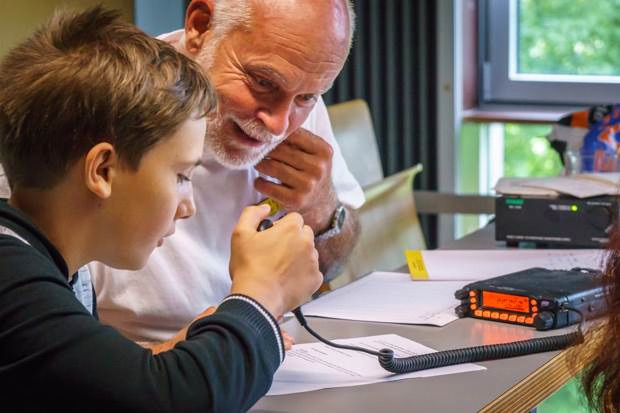
\includegraphics[width=0.85\textwidth]{foto/57}
    \caption{\scriptsize Ausbildungsfunkbetrieb verbindet oft die Generationen}
    \label{n_ausbildungsrufzeichen_ausbildungsfunkbetrieb}
\end{figure}

    \end{column}
   \begin{column}{0.48\textwidth}
       \begin{itemize}
  \item Funkamateure der Klasse~E und A sind automatisch Ausbilder
  \item Unter Aufsicht
  \item Im Berechtigungsumfang des Ausbilders
  \item Personengebundenes Rufzeichen + \enquote{/T} bzw. \enquote{/Trainee}
  \item Klubstation + \enquote{/T} bzw. \enquote{/Trainee}
  \end{itemize}

   \end{column}
\end{columns}

\end{frame}

\begin{frame}
\only<1>{
\begin{QQuestion}{VD302}{Unter welcher Voraussetzung nach der Amateurfunkverordnung (AFuV) darf ein Funkamateur Ausbildungsfunkbetrieb durchführen?}{Nur wenn er Inhaber einer Zulassung zur Teilnahme am Amateurfunkdienst der Klasse A ist}
{Wenn er Inhaber einer Zulassung zur Teilnahme am Amateurfunkdienst der Klasse A oder E ist}
{Nur wenn er mindestens 1 Jahr lang Inhaber einer Zulassung zur Teilnahme am Amateurfunkdienst ist}
{Wenn er eine gültige Rufzeichenzuteilung für ein Ausbildungsrufzeichen besitzt}
\end{QQuestion}

}
\only<2>{
\begin{QQuestion}{VD302}{Unter welcher Voraussetzung nach der Amateurfunkverordnung (AFuV) darf ein Funkamateur Ausbildungsfunkbetrieb durchführen?}{Nur wenn er Inhaber einer Zulassung zur Teilnahme am Amateurfunkdienst der Klasse A ist}
{\textbf{\textcolor{DARCgreen}{Wenn er Inhaber einer Zulassung zur Teilnahme am Amateurfunkdienst der Klasse A oder E ist}}}
{Nur wenn er mindestens 1 Jahr lang Inhaber einer Zulassung zur Teilnahme am Amateurfunkdienst ist}
{Wenn er eine gültige Rufzeichenzuteilung für ein Ausbildungsrufzeichen besitzt}
\end{QQuestion}

}
\end{frame}

\begin{frame}
\only<1>{
\begin{QQuestion}{BD211}{DG2RON führt Ausbildungsfunkbetrieb in Morsetelegrafie oder mit digitalen Übertragungsverfahren durch. Welches Rufzeichen hat der Auzubildende zu verwenden?}{DG2RON/A}
{T/DG2RON}
{DG2RON/T}
{A/DG2RON}
\end{QQuestion}

}
\only<2>{
\begin{QQuestion}{BD211}{DG2RON führt Ausbildungsfunkbetrieb in Morsetelegrafie oder mit digitalen Übertragungsverfahren durch. Welches Rufzeichen hat der Auzubildende zu verwenden?}{DG2RON/A}
{T/DG2RON}
{\textbf{\textcolor{DARCgreen}{DG2RON/T}}}
{A/DG2RON}
\end{QQuestion}

}
\end{frame}

\begin{frame}
\only<1>{
\begin{QQuestion}{VD304}{Was ist unter anderem im Zusammenhang mit der Durchführung von Ausbildungsfunkverkehr zu beachten? Der Ausbildungsfunkbetrieb darf~...}{nur mit einer maximalen Strahlungsleistung von \qty{10}{\W} EIRP durchgeführt werden.}
{nicht in Morsetelegrafie durchgeführt werden.}
{nur im Berechtigungsumfang der Rufzeichenzuteilung des Ausbilders durchgeführt werden.}
{nur an einer Klubstation durchgeführt werden.}
\end{QQuestion}

}
\only<2>{
\begin{QQuestion}{VD304}{Was ist unter anderem im Zusammenhang mit der Durchführung von Ausbildungsfunkverkehr zu beachten? Der Ausbildungsfunkbetrieb darf~...}{nur mit einer maximalen Strahlungsleistung von \qty{10}{\W} EIRP durchgeführt werden.}
{nicht in Morsetelegrafie durchgeführt werden.}
{\textbf{\textcolor{DARCgreen}{nur im Berechtigungsumfang der Rufzeichenzuteilung des Ausbilders durchgeführt werden.}}}
{nur an einer Klubstation durchgeführt werden.}
\end{QQuestion}

}
\end{frame}

\begin{frame}
\only<1>{
\begin{QQuestion}{BD210}{An der Klubstation DL0MOL soll Ausbildungsfunkbetrieb stattfinden. Darf der Auszubildende das Rufzeichen der Klubstation verwenden?}{Nein, es ist das persönliche Rufzeichen des Ausbilders zu verwenden.}
{Ja, wenn T/DL0MOL bzw. Trainee/DL0MOL verwendet wird.}
{Ja, wenn DL0MOL/T bzw. DL0MOL/Trainee verwendet wird.}
{Nein, an Klubstationen darf nicht ausgebildet werden.}
\end{QQuestion}

}
\only<2>{
\begin{QQuestion}{BD210}{An der Klubstation DL0MOL soll Ausbildungsfunkbetrieb stattfinden. Darf der Auszubildende das Rufzeichen der Klubstation verwenden?}{Nein, es ist das persönliche Rufzeichen des Ausbilders zu verwenden.}
{Ja, wenn T/DL0MOL bzw. Trainee/DL0MOL verwendet wird.}
{\textbf{\textcolor{DARCgreen}{Ja, wenn DL0MOL/T bzw. DL0MOL/Trainee verwendet wird.}}}
{Nein, an Klubstationen darf nicht ausgebildet werden.}
\end{QQuestion}

}
 \end{frame}

\begin{frame}
\frametitle{Ausbildungsfunkbetrieb ist …}
\begin{itemize}
  \item für Personen ohne Besitz eines entsprechenden Amateurfunkzeugnisses
  \item nicht für Aussendungen des Ausbilders selbst
  \item die praktische Vorbereitung auf das Ablegen der fachlichen Prüfung
  \end{itemize}
\end{frame}

\begin{frame}
\only<1>{
\begin{QQuestion}{VD301}{Wozu dient der Ausbildungsfunkbetrieb gemäß Amateurfunkverordnung (AFuV)? Er dient~...}{der alleinigen Vorführung des Amateurfunkbetriebes.}
{der praktischen Vorbereitung auf das Ablegen der fachlichen Prüfung zum Erwerb eines Amateurfunkzeugnisses.}
{der Teilnahme des Auszubildenden am Amateurfunkdienst ohne Aufsicht.}
{der Vervollständigung der Fertigkeiten des Funkamateurs in der Morsetelegrafie.}
\end{QQuestion}

}
\only<2>{
\begin{QQuestion}{VD301}{Wozu dient der Ausbildungsfunkbetrieb gemäß Amateurfunkverordnung (AFuV)? Er dient~...}{der alleinigen Vorführung des Amateurfunkbetriebes.}
{\textbf{\textcolor{DARCgreen}{der praktischen Vorbereitung auf das Ablegen der fachlichen Prüfung zum Erwerb eines Amateurfunkzeugnisses.}}}
{der Teilnahme des Auszubildenden am Amateurfunkdienst ohne Aufsicht.}
{der Vervollständigung der Fertigkeiten des Funkamateurs in der Morsetelegrafie.}
\end{QQuestion}

}
\end{frame}

\begin{frame}
\frametitle{Ausbilder …}
\begin{itemize}
  \item muss in unmittelbarer Nähe des Auszubildenden sein
  \item bei Bedienung und Betriebsabwicklung anleiten
  \item schaltet den Sender im Extremfall ab
  \item muss auf Verlangen der BNetzA Auskunft über \enquote{Art und Umfang} des Ausbildungsbetriebs geben
  \end{itemize}

\end{frame}

\begin{frame}
\only<1>{
\begin{QQuestion}{VD305}{Was ist bei der Durchführung von Ausbildungsfunkverkehr zu beachten?}{Der Ausbildungsfunkverkehr darf ausschließlich in Telefonie (SSB oder FM) durchgeführt werden.}
{Beim Ausbildungsfunkverkehr darf nicht an Amateurfunkwettbewerben teilgenommen werden.}
{Der Ausbildungsfunkverkehr darf ausschließlich in Gegenwart des Ausbilders an einer Klub- oder Schulstation durchgeführt werden.}
{Der  Ausbilder  hat  auf  Verlangen  der  Bundesnetzagentur  Auskunft  über  Art  und  Umfang  des 
Ausbildungsfunkbetriebs zu geben.}
\end{QQuestion}

}
\only<2>{
\begin{QQuestion}{VD305}{Was ist bei der Durchführung von Ausbildungsfunkverkehr zu beachten?}{Der Ausbildungsfunkverkehr darf ausschließlich in Telefonie (SSB oder FM) durchgeführt werden.}
{Beim Ausbildungsfunkverkehr darf nicht an Amateurfunkwettbewerben teilgenommen werden.}
{Der Ausbildungsfunkverkehr darf ausschließlich in Gegenwart des Ausbilders an einer Klub- oder Schulstation durchgeführt werden.}
{\textbf{\textcolor{DARCgreen}{Der  Ausbilder  hat  auf  Verlangen  der  Bundesnetzagentur  Auskunft  über  Art  und  Umfang  des 
Ausbildungsfunkbetriebs zu geben.}}}
\end{QQuestion}

}
 \end{frame}%ENDCONTENT


\section{Remote-Stationen}
\label{section:remote_stationen}
\begin{frame}%STARTCONTENT
\begin{itemize}
  \item Remotestationen ermöglichen einen Betrieb an einem anderen Standort
  \item z.B. wenn am Wohnort keine eigene Station realisiert werden kann
  \item Die gesamte Bedienung erfolgt ferngesteuert
  \end{itemize}
\begin{itemize}
  \item Betrieb durch Funkamateure der Klasse~A
  \item Mitbenutzung möglich
  \end{itemize}

\end{frame}

\begin{frame}
\only<1>{
\begin{QQuestion}{VD601}{Was versteht der Funkamateur unter \glqq Remote-Betrieb\grqq{}?}{Funkbetrieb bei Wettbewerben mit mehreren Funkamateuren mit verteilten Aufgaben}
{Funkbetrieb über sehr weite Entfernungen (größer \qty{500}{\km} UKW, größer \qty{2000}{\km} KW)}
{Die lokale Steuerung einer Funkstation über einen daneben stehenden Computer}
{Funkbetrieb, bei dem eine räumlich entfernte Amateurfunkstation z.~B. über das Internet betrieben wird}
\end{QQuestion}

}
\only<2>{
\begin{QQuestion}{VD601}{Was versteht der Funkamateur unter \glqq Remote-Betrieb\grqq{}?}{Funkbetrieb bei Wettbewerben mit mehreren Funkamateuren mit verteilten Aufgaben}
{Funkbetrieb über sehr weite Entfernungen (größer \qty{500}{\km} UKW, größer \qty{2000}{\km} KW)}
{Die lokale Steuerung einer Funkstation über einen daneben stehenden Computer}
{\textbf{\textcolor{DARCgreen}{Funkbetrieb, bei dem eine räumlich entfernte Amateurfunkstation z.~B. über das Internet betrieben wird}}}
\end{QQuestion}

}
\end{frame}

\begin{frame}
\only<1>{
\begin{QQuestion}{VD603}{Wer darf eine \glqq Remote-Station\grqq{} betreiben?}{Funkamateure der Klassen A und E}
{Funkamateure der Klasse A}
{Funkamateure der Klassen A, E und N}
{Funkamateure, die seit mindestens einem Jahr eine Zulassung besitzen}
\end{QQuestion}

}
\only<2>{
\begin{QQuestion}{VD603}{Wer darf eine \glqq Remote-Station\grqq{} betreiben?}{Funkamateure der Klassen A und E}
{\textbf{\textcolor{DARCgreen}{Funkamateure der Klasse A}}}
{Funkamateure der Klassen A, E und N}
{Funkamateure, die seit mindestens einem Jahr eine Zulassung besitzen}
\end{QQuestion}

}
\end{frame}

\begin{frame}
\only<1>{
\begin{QQuestion}{VD607}{Wer darf mit einer Amateurfunkstelle im \glqq Remote-Betrieb\grqq{} senden? Vom Betreiber der Amateurfunkstelle berechtigte Funkamateure, die ...}{über eine Zulassung für die Klasse~A, E oder N verfügen.}
{über eine Zulassung für die Klasse~A oder E verfügen.}
{über eine Zulassung für die Klasse~A verfügen.}
{seit mindestens einem Jahr über eine Zulassung verfügen.}
\end{QQuestion}

}
\only<2>{
\begin{QQuestion}{VD607}{Wer darf mit einer Amateurfunkstelle im \glqq Remote-Betrieb\grqq{} senden? Vom Betreiber der Amateurfunkstelle berechtigte Funkamateure, die ...}{über eine Zulassung für die Klasse~A, E oder N verfügen.}
{über eine Zulassung für die Klasse~A oder E verfügen.}
{\textbf{\textcolor{DARCgreen}{über eine Zulassung für die Klasse~A verfügen.}}}
{seit mindestens einem Jahr über eine Zulassung verfügen.}
\end{QQuestion}

}
\end{frame}

\begin{frame}
\frametitle{Betriebsmeldung}
\begin{itemize}
  \item Remotebetrieb muss durch den Betreiber angezeigt werden
  \item Mit Betriebsmeldung und Kontaktdaten an die BNetzA
  \item Erreichbarkeit während des Betriebs unter den angegebenen Kontaktdaten
  \end{itemize}

\end{frame}

\begin{frame}
\only<1>{
\begin{QQuestion}{VD602}{Ist für \glqq Remote-Betrieb\grqq{} bei der BNetzA eine Betriebsmeldung erforderlich?}{Ja, für Betreiber und Nutzer der Remote-Station}
{Ja, für den Nutzer der Remote-Station}
{Ja, für den Betreiber der Remote-Station}
{Nein, es besteht keine Anzeigepflicht.}
\end{QQuestion}

}
\only<2>{
\begin{QQuestion}{VD602}{Ist für \glqq Remote-Betrieb\grqq{} bei der BNetzA eine Betriebsmeldung erforderlich?}{Ja, für Betreiber und Nutzer der Remote-Station}
{Ja, für den Nutzer der Remote-Station}
{\textbf{\textcolor{DARCgreen}{Ja, für den Betreiber der Remote-Station}}}
{Nein, es besteht keine Anzeigepflicht.}
\end{QQuestion}

}
\end{frame}

\begin{frame}
\only<1>{
\begin{QQuestion}{VD608}{Warum muss der Betreiber der \glqq Remote-Station\grqq{} seine Kontaktdaten bei der BNetzA angeben?}{Die Bandwacht der Amateurfunkverbände nutzt die Kontaktdaten zum Datenabgleich, um im Störungsfall den Betreiber der \glqq Remote-Station\grqq{} zu ermitteln.}
{Die Kontaktdaten dienen der monatlichen Rechnungsstellung für die \glqq Remote-Station\grqq{}.}
{Der Betreiber muss für die BNetzA als Ansprechpartner erreichbar sein.}
{Die Kontaktdaten zum Remote-Betrieb werden in der Rufzeichenliste der BNetzA aufgeführt.}
\end{QQuestion}

}
\only<2>{
\begin{QQuestion}{VD608}{Warum muss der Betreiber der \glqq Remote-Station\grqq{} seine Kontaktdaten bei der BNetzA angeben?}{Die Bandwacht der Amateurfunkverbände nutzt die Kontaktdaten zum Datenabgleich, um im Störungsfall den Betreiber der \glqq Remote-Station\grqq{} zu ermitteln.}
{Die Kontaktdaten dienen der monatlichen Rechnungsstellung für die \glqq Remote-Station\grqq{}.}
{\textbf{\textcolor{DARCgreen}{Der Betreiber muss für die BNetzA als Ansprechpartner erreichbar sein.}}}
{Die Kontaktdaten zum Remote-Betrieb werden in der Rufzeichenliste der BNetzA aufgeführt.}
\end{QQuestion}

}
\end{frame}

\begin{frame}
\frametitle{Betriebssicherheit}
\begin{itemize}
  \item Ununterbrochene, mittelbare und vollständige Kontrolle der Station
  \item Kann über Hilfsmittel oder Helfer erfolgen
  \item Bei Störungen muss die Stationen in einen sicheren Zustand versetzt werden
  \end{itemize}

\end{frame}

\begin{frame}
\only<1>{
\begin{QQuestion}{VD605}{Wie muss der Betreiber die Betriebssicherheit seiner \glqq Remote-Station\grqq{} gewährleisten? Der Betreiber muss sicherstellen, dass~...}{die \glqq Remote-Station\grqq{} über eine unterbrechungsfreie Stromversorgung verfügt.}
{für die \glqq Remote-Station\grqq{} keine selbstgebauten Komponenten zum Einsatz kommen.}
{die \glqq Remote-Station\grqq{} unter seiner mittelbaren Kontrolle steht.}
{ein technisches Protokoll der Nutzung der \glqq Remote-Station\grqq{} erstellt wird.}
\end{QQuestion}

}
\only<2>{
\begin{QQuestion}{VD605}{Wie muss der Betreiber die Betriebssicherheit seiner \glqq Remote-Station\grqq{} gewährleisten? Der Betreiber muss sicherstellen, dass~...}{die \glqq Remote-Station\grqq{} über eine unterbrechungsfreie Stromversorgung verfügt.}
{für die \glqq Remote-Station\grqq{} keine selbstgebauten Komponenten zum Einsatz kommen.}
{\textbf{\textcolor{DARCgreen}{die \glqq Remote-Station\grqq{} unter seiner mittelbaren Kontrolle steht.}}}
{ein technisches Protokoll der Nutzung der \glqq Remote-Station\grqq{} erstellt wird.}
\end{QQuestion}

}
\end{frame}

\begin{frame}
\frametitle{Berechtigte Funkamateure}
\begin{itemize}
  \item Erlaubnis des Betreibers für Nutzung notwendig
  \item Betreiber darf nur berechtigte Funkamateure die Remotestation nutzen lassen
  \end{itemize}
\end{frame}

\begin{frame}
\only<1>{
\begin{QQuestion}{VD606}{Was ist bei der Übertragung des Nutzungsrechts an einer \glqq Remote-Station\grqq{} auf andere Funkamateure zu beachten?}{Der Betreiber muss sicherstellen, dass nur von ihm berechtigte Funkamateure die Station nutzen können.}
{Der Zugang für die Nutzung der \glqq Remote-Station\grqq{} muss für alle Funkamateure öffentlich sein.}
{Die Nutzer der \glqq Remote-Station\grqq{} dürfen keinen Ausbildungsfunkbetrieb durchführen.}
{Die Funkamateure müssen mindestens im Besitz einer Amateurfunkzulassung der Klasse~E sein.}
\end{QQuestion}

}
\only<2>{
\begin{QQuestion}{VD606}{Was ist bei der Übertragung des Nutzungsrechts an einer \glqq Remote-Station\grqq{} auf andere Funkamateure zu beachten?}{\textbf{\textcolor{DARCgreen}{Der Betreiber muss sicherstellen, dass nur von ihm berechtigte Funkamateure die Station nutzen können.}}}
{Der Zugang für die Nutzung der \glqq Remote-Station\grqq{} muss für alle Funkamateure öffentlich sein.}
{Die Nutzer der \glqq Remote-Station\grqq{} dürfen keinen Ausbildungsfunkbetrieb durchführen.}
{Die Funkamateure müssen mindestens im Besitz einer Amateurfunkzulassung der Klasse~E sein.}
\end{QQuestion}

}
\end{frame}

\begin{frame}
\frametitle{Klubstationen}
\begin{itemize}
  \item Klubstationen der Klasse~A dürfen als Remotestation betrieben werden
  \item Muss auf die Mitglieder der Gruppe von Funkamateuren begrenzt sein
  \end{itemize}
\end{frame}

\begin{frame}
\only<1>{
\begin{QQuestion}{VD604}{Welche der folgenden Amateurfunkstellen darf als \glqq Remote-Station\grqq{} verwendet werden?}{Amateurfunkstellen mit personengebundenem Rufzeichen der Klasse~N}
{Klubstationen der Klasse~E}
{Klubstationen der Klasse~A}
{Amateurfunkstellen mit personengebundenem Rufzeichen der Klasse~E}
\end{QQuestion}

}
\only<2>{
\begin{QQuestion}{VD604}{Welche der folgenden Amateurfunkstellen darf als \glqq Remote-Station\grqq{} verwendet werden?}{Amateurfunkstellen mit personengebundenem Rufzeichen der Klasse~N}
{Klubstationen der Klasse~E}
{\textbf{\textcolor{DARCgreen}{Klubstationen der Klasse~A}}}
{Amateurfunkstellen mit personengebundenem Rufzeichen der Klasse~E}
\end{QQuestion}

}
\end{frame}

\begin{frame}
\only<1>{
\begin{QQuestion}{VD609}{Wem darf Zugriff auf eine Klubstation im Remote-Betrieb eingeräumt werden?}{Nur Mitgliedern der Gruppe von Funkamateuren, die die Klubstation betreibt}
{Nur auf der Zuteilungsurkunde eingetragenen Mitgliedern der Gruppe von Funkamateuren}
{Nur bei der Bundesnetzagentur schriftlich oder elektronisch gemeldeten Funkamateuren}
{Nur Funkamateuren, die die Klubstation persönlich nicht aufsuchen können}
\end{QQuestion}

}
\only<2>{
\begin{QQuestion}{VD609}{Wem darf Zugriff auf eine Klubstation im Remote-Betrieb eingeräumt werden?}{\textbf{\textcolor{DARCgreen}{Nur Mitgliedern der Gruppe von Funkamateuren, die die Klubstation betreibt}}}
{Nur auf der Zuteilungsurkunde eingetragenen Mitgliedern der Gruppe von Funkamateuren}
{Nur bei der Bundesnetzagentur schriftlich oder elektronisch gemeldeten Funkamateuren}
{Nur Funkamateuren, die die Klubstation persönlich nicht aufsuchen können}
\end{QQuestion}

}
\end{frame}

\begin{frame}
\frametitle{Ausbildungsfunkbetrieb}
\begin{itemize}
  \item Ist an einer Remotestation möglich
  \item Es gelten die gleichen Regeln wie für den Ausbildungsbetrieb
  \item Auch an Remote-Klubstationen möglich
  \end{itemize}

\end{frame}%ENDCONTENT


\section{Rufzeichenzusätze}
\label{section:rufzeichenzusaetze}
\begin{frame}%STARTCONTENT
Beim Funken von einem Standort anders als dem in der Zulassungsurkunde angegebenen Heimatstandort, kann ein Rufzeichenzusatz verwendet werden.

\end{frame}

\begin{frame}\begin{table}
\begin{DARCtabular}{lll}
     Zusatz  & Gesprochen  & Bedeutung   \\
     am  & aeronautisch mobil  & An Bord eines Luftfahrzeugst, das sich im Flug befindet   \\
     mm  & maritim mobil  & An Bord eines Schiffs auf See   \\
     m  & mobil  & Von einem Landfahrzeug oder einem Schiff auf Binnengewässern aus   \\
     p  & portabel  & Zu Fuß unterwegs oder vorübergehend ortsfest   \\
     R  & Remote  & Remote-Betrieb   \\
     T  & Trainee  & Ausbildungsfunk   \\
\end{DARCtabular}
\caption{Mögliche Rufzeichenzusätze}
\label{n_rufzeichenzusaetze}
\end{table}

\end{frame}

\begin{frame}\begin{itemize}
  \item Geschrieben mit \enquote{/}
  \item Gesprochen direkt im Anschluss an das Rufzeichen oder mit \enquote{Stroke}
  \end{itemize}
    \pause
    \begin{table}
\begin{DARCtabular}{lX}
     Schreibweise  & Aussprache   \\
     DL1FLO/m  & Delta Lima Eins Foxtrott Lima Oskar (Stroke) Mobil   \\
     DM4EAX/p  & Delta Mike Vier Echo Alpha X-Ray (Stroke) Portabel   \\
     DL1ASN/mm  & Delta Lima Eins Alpha Sierra November (Stroke) Maritim Mobil   \\
     DG2RON/am  & Delta Golf Zwei Romeo Oscar November (Stroke) Aeronautisch Mobil   \\
\end{DARCtabular}
\caption{Sprechweise von Rufzeichenzusätzen, "Stroke" ist optional und kann weggelassen werden}
\label{n_rufzeichenzusaetze_sprechweise}
\end{table}


\end{frame}

\begin{frame}
\frametitle{Aeronautisch Mobil}
\begin{itemize}
  \item An Bord eines Luftfahrzeugs (Flugzeug, Heißluftballon, Zeppelin, o.ä.)
  \item Muss sich komplett in der Luft befinden
  \item Keine Verbindung zum Boden
  \item Betrieb muss vom Luftfahrzeugführer erlaubt sein, jedoch nicht von der BNetzA genehmigt werden
  \end{itemize}
\end{frame}

\begin{frame}
\only<1>{
\begin{QQuestion}{BD201}{Was bedeutet der Rufzeichenzusatz \glqq /am\grqq{}? Die Amateurfunkstelle~...}{verwendet Amplitudenmodulation.}
{wird an Bord eines Luftfahrzeugs betrieben.}
{wird an Bord eines Wasserfahrzeugs betrieben.}
{arbeitet mit geringer Leistung.}
\end{QQuestion}

}
\only<2>{
\begin{QQuestion}{BD201}{Was bedeutet der Rufzeichenzusatz \glqq /am\grqq{}? Die Amateurfunkstelle~...}{verwendet Amplitudenmodulation.}
{\textbf{\textcolor{DARCgreen}{wird an Bord eines Luftfahrzeugs betrieben.}}}
{wird an Bord eines Wasserfahrzeugs betrieben.}
{arbeitet mit geringer Leistung.}
\end{QQuestion}

}
\end{frame}

\begin{frame}
\only<1>{
\begin{QQuestion}{BD202}{Welche Bedeutung hat das Rufzeichen VE8ZZ/am?}{Es handelt sich um eine kanadische Amateurfunkstelle, die vorübergehend in den Vereinigten Staaten von Amerika betrieben wird.}
{Es handelt sich um eine Amateurfunkstelle mit einem kanadischen Rufzeichen, die in einem Luftfahrzeug betrieben wird.}
{Es handelt sich um eine kanadische Amateurfunkstelle, die in der Modulationsart AM betrieben wird.}
{Es handelt sich um eine automatisch arbeitende Pactor-Amateurfunkstelle mit angeschlossener Mailbox in Kanada.}
\end{QQuestion}

}
\only<2>{
\begin{QQuestion}{BD202}{Welche Bedeutung hat das Rufzeichen VE8ZZ/am?}{Es handelt sich um eine kanadische Amateurfunkstelle, die vorübergehend in den Vereinigten Staaten von Amerika betrieben wird.}
{\textbf{\textcolor{DARCgreen}{Es handelt sich um eine Amateurfunkstelle mit einem kanadischen Rufzeichen, die in einem Luftfahrzeug betrieben wird.}}}
{Es handelt sich um eine kanadische Amateurfunkstelle, die in der Modulationsart AM betrieben wird.}
{Es handelt sich um eine automatisch arbeitende Pactor-Amateurfunkstelle mit angeschlossener Mailbox in Kanada.}
\end{QQuestion}

}
\end{frame}

\begin{frame}
\only<1>{
\begin{QQuestion}{VE705}{Welche Voraussetzung muss erfüllt sein, damit Sie Amateurfunk an Bord eines Luftfahrzeugs betreiben dürfen?}{Genehmigung der Bundesnetzagentur für aeronautischen Funkbetrieb}
{Zustimmung des verantwortlichen Luftfahrzeugführers}
{Verwendung einer fest installierten Funkstelle des mobilen Flugfunkdienstes}
{Nutzung von Frequenzen, die dem mobilen Flugfunkdienst zugewiesen sind}
\end{QQuestion}

}
\only<2>{
\begin{QQuestion}{VE705}{Welche Voraussetzung muss erfüllt sein, damit Sie Amateurfunk an Bord eines Luftfahrzeugs betreiben dürfen?}{Genehmigung der Bundesnetzagentur für aeronautischen Funkbetrieb}
{\textbf{\textcolor{DARCgreen}{Zustimmung des verantwortlichen Luftfahrzeugführers}}}
{Verwendung einer fest installierten Funkstelle des mobilen Flugfunkdienstes}
{Nutzung von Frequenzen, die dem mobilen Flugfunkdienst zugewiesen sind}
\end{QQuestion}

}
\end{frame}

\begin{frame}
\frametitle{Maritim Mobil}
\begin{itemize}
  \item An Bord eines Wasserfahrzeugs (Motorboot, Segelyacht, o.ä.)
  \item Außerhalb der 12-Meilen-Zone
  \item Auf Flüssen, Seen oder ähnlichen Binnengewässern darf \enquote{/m} (mobil) verwendet werden
  \item Betrieb muss vom Schiffsführer erlaubt sein, jedoch nicht von der BNetzA genehmigt werden
  \end{itemize}
\end{frame}

\begin{frame}
\only<1>{
\begin{QQuestion}{BD205}{Was ist aus dem Rufzeichen DC4LW/mm hinsichtlich des Betriebsortes zu erkennen? Die deutsche Amateurfunkstelle DC4LW~...}{wird von einem Schiff aus betrieben, das sich auf einem Binnengewässer befindet.}
{wird an Bord eines Wasserfahrzeugs betrieben, das sich auf See befindet.}
{möchte mit anderen Funkamateuren in Kontakt treten, die ihre Funkstelle zur Zeit auch \glqq maritim mobil\grqq{} betreiben.}
{wird an Bord eines Schiffes als eine mobile Station des See- und Binnenschifffahrtsfunks betrieben.}
\end{QQuestion}

}
\only<2>{
\begin{QQuestion}{BD205}{Was ist aus dem Rufzeichen DC4LW/mm hinsichtlich des Betriebsortes zu erkennen? Die deutsche Amateurfunkstelle DC4LW~...}{wird von einem Schiff aus betrieben, das sich auf einem Binnengewässer befindet.}
{\textbf{\textcolor{DARCgreen}{wird an Bord eines Wasserfahrzeugs betrieben, das sich auf See befindet.}}}
{möchte mit anderen Funkamateuren in Kontakt treten, die ihre Funkstelle zur Zeit auch \glqq maritim mobil\grqq{} betreiben.}
{wird an Bord eines Schiffes als eine mobile Station des See- und Binnenschifffahrtsfunks betrieben.}
\end{QQuestion}

}
\end{frame}

\begin{frame}
\only<1>{
\begin{QQuestion}{VE706}{Darf eine Amateurfunkstelle auch an Bord eines Schiffes, welches sich in internationalen Gewässern befindet, betrieben werden?}{Ja, mit der Zustimmung des Schiffsführers}
{Ja, mit der Zustimmung eines beliebigen Crewmitglieds}
{Ja, mit einer Genehmigung der BNetzA}
{Ja, mit einer Genehmigung des Bundesamtes für Seeschifffahrt und Hydrographie}
\end{QQuestion}

}
\only<2>{
\begin{QQuestion}{VE706}{Darf eine Amateurfunkstelle auch an Bord eines Schiffes, welches sich in internationalen Gewässern befindet, betrieben werden?}{\textbf{\textcolor{DARCgreen}{Ja, mit der Zustimmung des Schiffsführers}}}
{Ja, mit der Zustimmung eines beliebigen Crewmitglieds}
{Ja, mit einer Genehmigung der BNetzA}
{Ja, mit einer Genehmigung des Bundesamtes für Seeschifffahrt und Hydrographie}
\end{QQuestion}

}
\end{frame}

\begin{frame}
\only<1>{
\begin{QQuestion}{VD115}{Ist für den Betrieb einer Amateurfunkstelle in einem Wasser- oder Luftfahrzeug eine Sondergenehmigung der Bundesnetzagentur erforderlich?}{Es ist keine Sondergenehmigung  erforderlich.}
{Wenn der Funkamateur auch Inhaber eines Flugfunk- oder Seefunkzeugnisses ist, benötigt er keine Sondergenehmigung.}
{Es ist in jedem Fall eine Sondergenehmigung erforderlich.}
{Bei Strahlungsleistungen von über \qty{10}{\W} EIRP ist eine Sondergenehmigung erforderlich.}
\end{QQuestion}

}
\only<2>{
\begin{QQuestion}{VD115}{Ist für den Betrieb einer Amateurfunkstelle in einem Wasser- oder Luftfahrzeug eine Sondergenehmigung der Bundesnetzagentur erforderlich?}{\textbf{\textcolor{DARCgreen}{Es ist keine Sondergenehmigung  erforderlich.}}}
{Wenn der Funkamateur auch Inhaber eines Flugfunk- oder Seefunkzeugnisses ist, benötigt er keine Sondergenehmigung.}
{Es ist in jedem Fall eine Sondergenehmigung erforderlich.}
{Bei Strahlungsleistungen von über \qty{10}{\W} EIRP ist eine Sondergenehmigung erforderlich.}
\end{QQuestion}

}
\end{frame}

\begin{frame}
\frametitle{Mobil}
\begin{itemize}
  \item In einem Landfahrzeug wie Auto oder Zug
  \item Oder an Bord eines Schiffs auf Binnengewässern
  \end{itemize}
\end{frame}

\begin{frame}
\only<1>{
\begin{QQuestion}{BD203}{Ein Rufzeichen mit dem Zusatz \glqq /m\grqq{} kann bei einer Amateurfunkstelle bedeuten, dass sie~...}{vorübergehend ortsfest betrieben wird oder tragbar ist.}
{mit minimaler Leistung sendet.}
{beweglich ist und sich in einem Landfahrzeug befindet.}
{an Bord eines Wasserfahrzeugs betrieben wird, das sich auf See befindet.}
\end{QQuestion}

}
\only<2>{
\begin{QQuestion}{BD203}{Ein Rufzeichen mit dem Zusatz \glqq /m\grqq{} kann bei einer Amateurfunkstelle bedeuten, dass sie~...}{vorübergehend ortsfest betrieben wird oder tragbar ist.}
{mit minimaler Leistung sendet.}
{\textbf{\textcolor{DARCgreen}{beweglich ist und sich in einem Landfahrzeug befindet.}}}
{an Bord eines Wasserfahrzeugs betrieben wird, das sich auf See befindet.}
\end{QQuestion}

}
\end{frame}

\begin{frame}
\only<1>{
\begin{QQuestion}{BD204}{Ein Rufzeichen mit dem Zusatz \glqq /m\grqq{} kann bei einer Amateurfunkstelle bedeuten, dass sie~...}{an Bord eines Wasserfahrzeugs betrieben wird, das sich auf See befindet.}
{mit minimaler Leistung sendet.}
{vorübergehend ortsfest betrieben wird oder tragbar ist.}
{sich an Bord eines Wasserfahrzeugs auf Binnengewässern befindet.}
\end{QQuestion}

}
\only<2>{
\begin{QQuestion}{BD204}{Ein Rufzeichen mit dem Zusatz \glqq /m\grqq{} kann bei einer Amateurfunkstelle bedeuten, dass sie~...}{an Bord eines Wasserfahrzeugs betrieben wird, das sich auf See befindet.}
{mit minimaler Leistung sendet.}
{vorübergehend ortsfest betrieben wird oder tragbar ist.}
{\textbf{\textcolor{DARCgreen}{sich an Bord eines Wasserfahrzeugs auf Binnengewässern befindet.}}}
\end{QQuestion}

}
\end{frame}

\begin{frame}
\frametitle{Portabel}
\begin{itemize}
  \item Station vorübergehend an einem Standort, der nicht auf der Zuteilungsurkunde eingetragen ist
  \item z.B. in der Natur
  \item Auch bei Bewegung (zu Fuß) mit tragbarem Funkgerät
  \end{itemize}
\end{frame}

\begin{frame}
\only<1>{
\begin{QQuestion}{BD206}{Was bedeutet der Rufzeichenzusatz \glqq /p\grqq{}? Es bedeutet, dass die Amateurfunkstelle~...}{sich an Bord eines Wasserfahrzeugs auf See befindet.}
{sich in einem Landfahrzeug in Bewegung befindet.}
{vorübergehend exterritorial betrieben wird.}
{vorübergehend ortsfest betrieben wird oder tragbar ist.}
\end{QQuestion}

}
\only<2>{
\begin{QQuestion}{BD206}{Was bedeutet der Rufzeichenzusatz \glqq /p\grqq{}? Es bedeutet, dass die Amateurfunkstelle~...}{sich an Bord eines Wasserfahrzeugs auf See befindet.}
{sich in einem Landfahrzeug in Bewegung befindet.}
{vorübergehend exterritorial betrieben wird.}
{\textbf{\textcolor{DARCgreen}{vorübergehend ortsfest betrieben wird oder tragbar ist.}}}
\end{QQuestion}

}
\end{frame}

\begin{frame}
\only<1>{
\begin{QQuestion}{BD207}{Muss beim Betrieb einer tragbaren oder vorübergehend ortsfest betriebenen Amateurfunkstelle in Deutschland dem Rufzeichen der Zusatz \glqq /p\grqq{} hinzugefügt werden?}{Nein, es sei denn, es handelt sich um eine ausländische Station.}
{Ja, damit die BNetzA erkennen kann, dass die Amateurfunkstelle nicht am gemeldeten Standort betrieben wird.}
{Ja, weil dies durch die internationalen Regelungen in den Radio Regulations (RR) so vorgegeben ist.}
{Nein, er kann zur weiteren Information verwendet werden.}
\end{QQuestion}

}
\only<2>{
\begin{QQuestion}{BD207}{Muss beim Betrieb einer tragbaren oder vorübergehend ortsfest betriebenen Amateurfunkstelle in Deutschland dem Rufzeichen der Zusatz \glqq /p\grqq{} hinzugefügt werden?}{Nein, es sei denn, es handelt sich um eine ausländische Station.}
{Ja, damit die BNetzA erkennen kann, dass die Amateurfunkstelle nicht am gemeldeten Standort betrieben wird.}
{Ja, weil dies durch die internationalen Regelungen in den Radio Regulations (RR) so vorgegeben ist.}
{\textbf{\textcolor{DARCgreen}{Nein, er kann zur weiteren Information verwendet werden.}}}
\end{QQuestion}

}
\end{frame}

\begin{frame}
\frametitle{Remote}
\begin{itemize}
  \item Betrieb an einer Remote-Station
  \item Optional \enquote{/R} bzw. \enquote{/Remote}
  \end{itemize}
\end{frame}

\begin{frame}
\only<1>{
\begin{QQuestion}{BD208}{Welcher Rufzeichenzusatz kann verwendet werden, um \glqq Remote-Betrieb\grqq{} zu kennzeichnen?}{/RB bzw. /Remotebetrieb}
{/R bzw. /Remote}
{/FB bzw. /Fernbedient}
{/F bzw. /Fern}
\end{QQuestion}

}
\only<2>{
\begin{QQuestion}{BD208}{Welcher Rufzeichenzusatz kann verwendet werden, um \glqq Remote-Betrieb\grqq{} zu kennzeichnen?}{/RB bzw. /Remotebetrieb}
{\textbf{\textcolor{DARCgreen}{/R bzw. /Remote}}}
{/FB bzw. /Fernbedient}
{/F bzw. /Fern}
\end{QQuestion}

}
\end{frame}

\begin{frame}
\frametitle{Trainee}
\begin{itemize}
  \item Bei Ausbildungsfunkbetrieb ist \enquote{/T} bzw. \enquote{/Trainee} verpflichtend
  \item Alle anderen Zusätze sind freiwillig und können weggelassen werden
  \end{itemize}
\end{frame}

\begin{frame}
\only<1>{
\begin{QQuestion}{BD209}{Der Funkamateur mit dem Rufzeichen DL1PZ möchte Ausbildungsfunkbetrieb im Sprechfunk durchführen. Welches Rufzeichen darf der Auszubildende verwenden?}{DL1PZ/Trainee}
{DL1PZ/Ausbildung}
{Ausbildung/DL1PZ}
{Trainee/DL1PZ}
\end{QQuestion}

}
\only<2>{
\begin{QQuestion}{BD209}{Der Funkamateur mit dem Rufzeichen DL1PZ möchte Ausbildungsfunkbetrieb im Sprechfunk durchführen. Welches Rufzeichen darf der Auszubildende verwenden?}{\textbf{\textcolor{DARCgreen}{DL1PZ/Trainee}}}
{DL1PZ/Ausbildung}
{Ausbildung/DL1PZ}
{Trainee/DL1PZ}
\end{QQuestion}

}
\end{frame}

\begin{frame}
\only<1>{
\begin{QQuestion}{VD306}{Von wem ist während des Ausbildungsfunkbetriebs der Rufzeichenzusatz \glqq /T\grqq{} bzw. \glqq /Trainee\grqq{} zu benutzen?}{Vom Verantwortlichen der Schulstation}
{Vom Ausbilder}
{Vom Auszubildenden und vom Ausbilder}
{Vom Auszubildenden}
\end{QQuestion}

}
\only<2>{
\begin{QQuestion}{VD306}{Von wem ist während des Ausbildungsfunkbetriebs der Rufzeichenzusatz \glqq /T\grqq{} bzw. \glqq /Trainee\grqq{} zu benutzen?}{Vom Verantwortlichen der Schulstation}
{Vom Ausbilder}
{Vom Auszubildenden und vom Ausbilder}
{\textbf{\textcolor{DARCgreen}{Vom Auszubildenden}}}
\end{QQuestion}

}
\end{frame}

\begin{frame}
\only<1>{
\begin{QQuestion}{BD210}{An der Klubstation DL0MOL soll Ausbildungsfunkbetrieb stattfinden. Darf der Auszubildende das Rufzeichen der Klubstation verwenden?}{Nein, es ist das persönliche Rufzeichen des Ausbilders zu verwenden.}
{Ja, wenn T/DL0MOL bzw. Trainee/DL0MOL verwendet wird.}
{Ja, wenn DL0MOL/T bzw. DL0MOL/Trainee verwendet wird.}
{Nein, an Klubstationen darf nicht ausgebildet werden.}
\end{QQuestion}

}
\only<2>{
\begin{QQuestion}{BD210}{An der Klubstation DL0MOL soll Ausbildungsfunkbetrieb stattfinden. Darf der Auszubildende das Rufzeichen der Klubstation verwenden?}{Nein, es ist das persönliche Rufzeichen des Ausbilders zu verwenden.}
{Ja, wenn T/DL0MOL bzw. Trainee/DL0MOL verwendet wird.}
{\textbf{\textcolor{DARCgreen}{Ja, wenn DL0MOL/T bzw. DL0MOL/Trainee verwendet wird.}}}
{Nein, an Klubstationen darf nicht ausgebildet werden.}
\end{QQuestion}

}
\end{frame}%ENDCONTENT


\section{Besondere Anlässe}
\label{section:besondere_anlaesse}
\begin{frame}%STARTCONTENT

\begin{columns}
    \begin{column}{0.48\textwidth}
    
\begin{figure}
    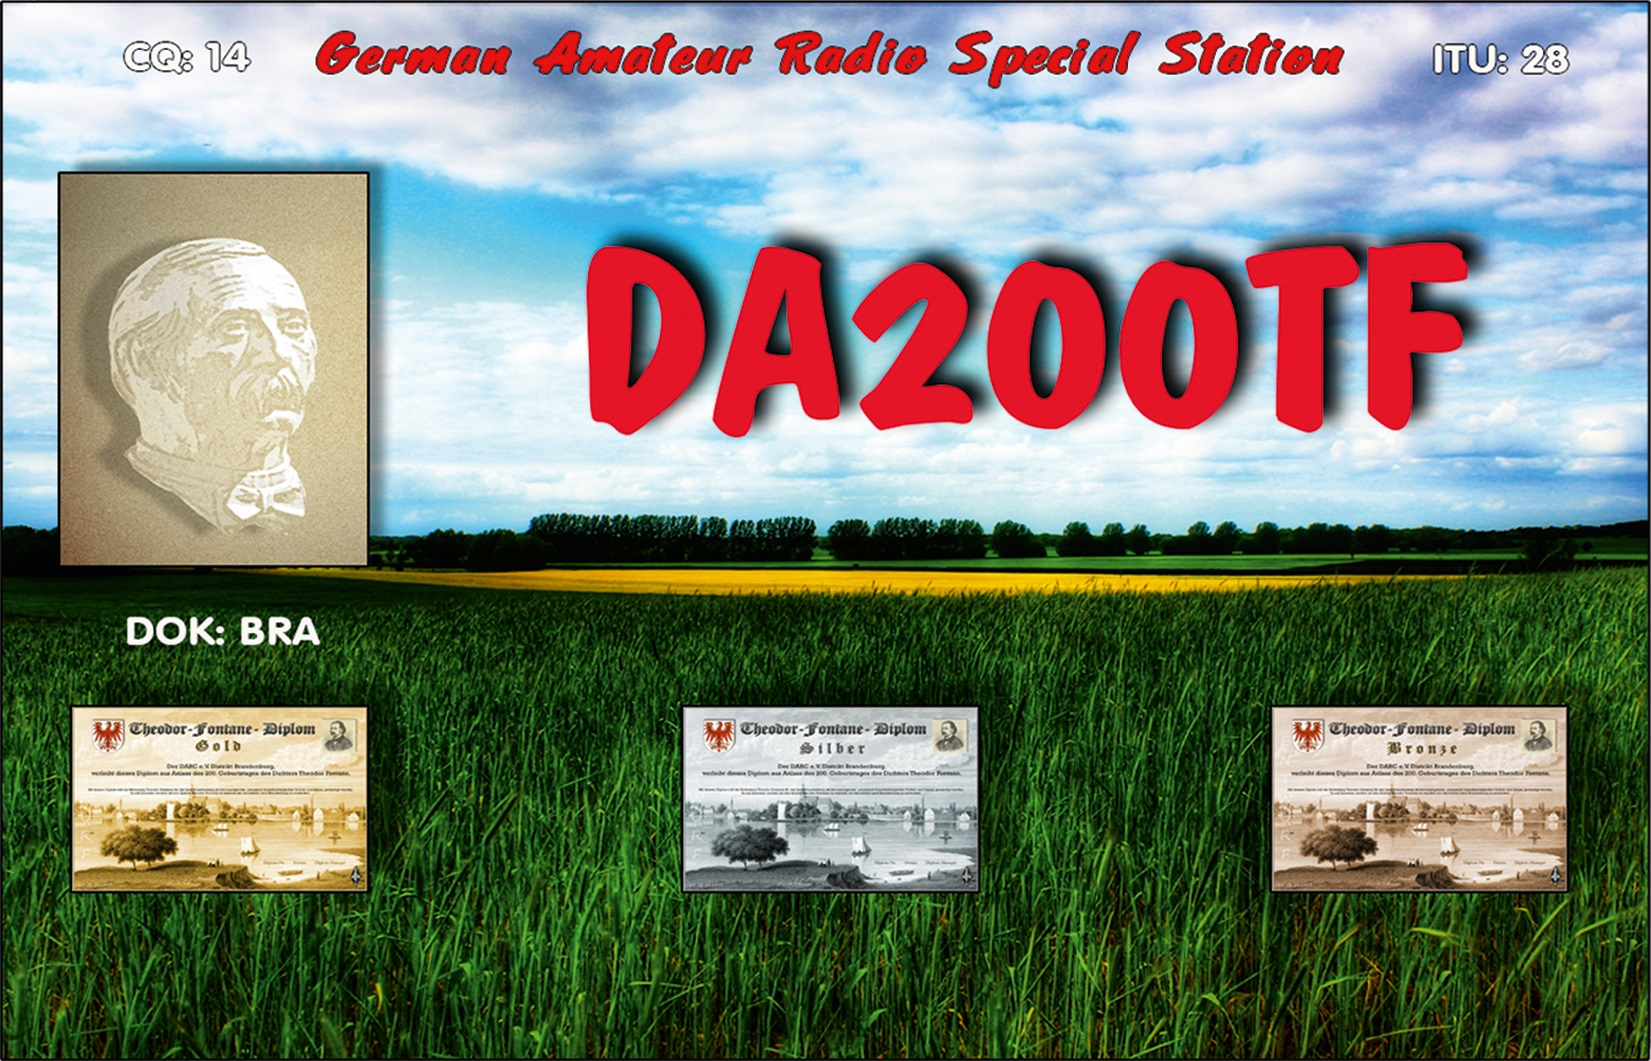
\includegraphics[width=0.85\textwidth]{foto/59}
    \caption{\scriptsize QSL-Karte der Klubstation mit dem Sonderrufzeichen DA200TF anlässlich des 200. Geburtstag von Theodor Fontane}
    \label{n_besondere_anlaesse_qsl_karte_DA200TF}
\end{figure}

    \end{column}
   \begin{column}{0.48\textwidth}
       \begin{itemize}
  \item Klubstationsrufzeichen mit 4-7stelligem Suffix
  \item z.B. für historische Ereignisse, Stadtfeste oder Sportereignisse
  \item Die ganze Amateurfunkwelt kann an dem Ereignis teilhaben
  \end{itemize}

   \end{column}
\end{columns}

\end{frame}

\begin{frame}
\frametitle{Vorgaben}
\begin{itemize}
  \item Maximale Zuweisung für 1 Jahr durch die BNetzA
  \item Keine Verlängerung möglich
  \item Suffix kann aus Ziffern und Buchstaben bestehen
  \item Das letzte Zeichen muss immer ein Buchstabe sein
  \end{itemize}
\end{frame}

\begin{frame}
\frametitle{International}
\begin{itemize}
  \item Auch im Ausland kann es Sonderstationen geben
  \item Die Rufzeichen können andere Vorgaben haben
  \end{itemize}
\end{frame}

\begin{frame}\begin{table}
\begin{DARCtabular}{llX}
     Rufzeichen  & Zuteilung  & Ereignis   \\
     DL1250BRET  & 2017  & 1250 Jahre Stadt Bretten   \\
     DL500BIER  & 2016  & 500 Jahre Deutsches Reinheitsgebot   \\
     DF13DEJU  & 2019  & Erstflug der Junkers F 13   \\
     DL73AFUG  & 2022  & 73. Geburtstags des Amateurfunkgesetzes   \\
     DB50AFZ  & 2022  & 50 Jahre Amateurfunkzentrum   \\
     DP44N44T  & 2022  & 44 Jahre Ortsverband N44   \\
     DC0YOTA  & 2021  & Youngsters On The Air   \\
     DL22MAUS  & 2022  & Türen auf mit der Maus!   \\
     DL0ELEFANT  & 2022  & Türen auf mit der Maus!   \\
\end{DARCtabular}
\caption{Beispiele für Sonderstationen}
\label{n_besondere_anlaesse}
\end{table}

\end{frame}

\begin{frame}
\only<1>{
\begin{QQuestion}{VD204}{Warum ist \glqq DL250BTHVN\grqq{} ein zulässiges deutsches Amateurfunkrufzeichen?}{Weil für besonders verdiente Funkamateure auch personengebundene Rufzeichen ausgegeben werden, für die der Rufzeichenplan keine Anwendung findet.}
{Weil der Rufzeichenplan zu besonderen allgemeinen Anlässen auch Rufzeichen mit bis zu 7 Zeichen langem Suffix vorsieht, der Ziffern enthalten kann und mit einem Buchstaben endet.}
{Weil an bestimmte öffentliche Stellen, wie z.~B. Kunst- und Kultureinrichtungen, besondere Rufzeichen mit mindestens 3 Ziffern ausgegeben werden.}
{Weil dies in einer Sonderverfügung der Bundesnetzagentur aufgrund besonderen historischen Anlass mit internationaler Wirkung festgelegt wurde.}
\end{QQuestion}

}
\only<2>{
\begin{QQuestion}{VD204}{Warum ist \glqq DL250BTHVN\grqq{} ein zulässiges deutsches Amateurfunkrufzeichen?}{Weil für besonders verdiente Funkamateure auch personengebundene Rufzeichen ausgegeben werden, für die der Rufzeichenplan keine Anwendung findet.}
{\textbf{\textcolor{DARCgreen}{Weil der Rufzeichenplan zu besonderen allgemeinen Anlässen auch Rufzeichen mit bis zu 7 Zeichen langem Suffix vorsieht, der Ziffern enthalten kann und mit einem Buchstaben endet.}}}
{Weil an bestimmte öffentliche Stellen, wie z.~B. Kunst- und Kultureinrichtungen, besondere Rufzeichen mit mindestens 3 Ziffern ausgegeben werden.}
{Weil dies in einer Sonderverfügung der Bundesnetzagentur aufgrund besonderen historischen Anlass mit internationaler Wirkung festgelegt wurde.}
\end{QQuestion}

}
\end{frame}%ENDCONTENT


\section{Fernbediente und automatische Stationen}
\label{section:fernbediente_automatische_stationen}
\begin{frame}%STARTCONTENT

\frametitle{Normalerweise}
\begin{itemize}
  \item Funkamateur muss die Station besetzt betreiben
  \item Aussendungen dürfen nur unter Aufsicht erfolgen
  \item Direkt an der Sendeanlage oder mittelbar via Remote-Station
  \end{itemize}
    \pause
    Ausnahme: Fernbediente und automatische Stationen



\end{frame}

\begin{frame}
\frametitle{Relaisfunkstelle}
\begin{itemize}
  \item Ermöglicht Funverbindungen zwischen Funkamateuren, die sich nicht direkt erreichen können
  \item Sendet alles, was sie auf einer Frequenz empfängt, auf einer anderen wieder aus
  \end{itemize}

\end{frame}

\begin{frame}
\frametitle{Bake}
\begin{itemize}
  \item Sendet nur immer das gleiche
  \item In regelmäßigen Abständen
  \item Oftmals nur das Rufzeichen
  \item Zur Untersuchung der Ausbreitungsbedingungen
  \end{itemize}
\end{frame}

\begin{frame}
\only<1>{
\begin{QQuestion}{VD501}{Was ist notwendig, damit ein Funkamateur eine Amateurfunkstelle als Relaisfunkstelle oder Funkbake betreiben darf?}{Es ist eine Zulassung der höchsten Amateurfunkklasse erforderlich.}
{Es bedarf einer Rufzeichenzuteilung für den Betrieb einer fernbedienten oder automatisch arbeitenden Amateurfunkstelle.}
{Für den Betrieb einer Relaisfunkstelle oder Funkbake ist der mindestens 2-jährige Besitz einer gültigen Amateurfunkzulassung erforderlich.}
{Es sind keine besonderen Bedingungen zu erfüllen.}
\end{QQuestion}

}
\only<2>{
\begin{QQuestion}{VD501}{Was ist notwendig, damit ein Funkamateur eine Amateurfunkstelle als Relaisfunkstelle oder Funkbake betreiben darf?}{Es ist eine Zulassung der höchsten Amateurfunkklasse erforderlich.}
{\textbf{\textcolor{DARCgreen}{Es bedarf einer Rufzeichenzuteilung für den Betrieb einer fernbedienten oder automatisch arbeitenden Amateurfunkstelle.}}}
{Für den Betrieb einer Relaisfunkstelle oder Funkbake ist der mindestens 2-jährige Besitz einer gültigen Amateurfunkzulassung erforderlich.}
{Es sind keine besonderen Bedingungen zu erfüllen.}
\end{QQuestion}

}
\end{frame}

\begin{frame}
\only<1>{
\begin{QQuestion}{VD502}{Unter welchen Voraussetzungen darf ein Funkamateur eine Amateurfunkstelle als Relaisfunkstelle betreiben?}{Wenn die Relaisfunkstelle keine große Reichweite hat}
{Wenn er für die Relaisfunkstelle eine Rufzeichenzuteilung besitzt und die darin festgelegten Rahmenbedingungen einhält}
{Wenn er mindestens 20 Unterschriften als Beweis der Notwendigkeit vorlegen kann und die Rahmenbedingungen für Relaisfunkstellen einhält}
{Wenn er die technischen Einrichtungen dafür selbst instand halten kann}
\end{QQuestion}

}
\only<2>{
\begin{QQuestion}{VD502}{Unter welchen Voraussetzungen darf ein Funkamateur eine Amateurfunkstelle als Relaisfunkstelle betreiben?}{Wenn die Relaisfunkstelle keine große Reichweite hat}
{\textbf{\textcolor{DARCgreen}{Wenn er für die Relaisfunkstelle eine Rufzeichenzuteilung besitzt und die darin festgelegten Rahmenbedingungen einhält}}}
{Wenn er mindestens 20 Unterschriften als Beweis der Notwendigkeit vorlegen kann und die Rahmenbedingungen für Relaisfunkstellen einhält}
{Wenn er die technischen Einrichtungen dafür selbst instand halten kann}
\end{QQuestion}

}
\end{frame}%ENDCONTENT


\section{Relaisfunkstellen}
\label{section:relaisfunkstellen}
\begin{frame}%STARTCONTENT

\begin{columns}
    \begin{column}{0.48\textwidth}
    
\begin{figure}
    \DARCimage{0.85\linewidth}{648include}
    \caption{\scriptsize Schematische Darstellung einer Relaisfunkstelle mit Nutzern}
    \label{n_relaisfunkstellen_aufbau}
\end{figure}


    \end{column}
   \begin{column}{0.48\textwidth}
       \begin{itemize}
  \item Ermöglicht eine größere Reichweite als bei direkter Verbindung
  \item Meist an exponierten Standorten, z.B. Berggipfeln, Hochhäusern, (Kirch-)Türmen
  \item Oder in Satelliten
  \end{itemize}

   \end{column}
\end{columns}

\end{frame}

\begin{frame}
\frametitle{Definition Relaisfunkstelle}
eine fernbediente Amateurfunkstelle (auch in Satelliten), die empfangene Amateurfunkaussendungen, Teile davon oder sonstige eingespeiste oder eingespeicherte Signale fern ausgelöst aussendet und dabei zur Erhöhung der Erreichbarkeit von Amateurfunkstellen dient

\end{frame}

\begin{frame}
\begin{columns}
    \begin{column}{0.48\textwidth}
    \begin{itemize}
  \item Auch kurz genannt: Relais oder Repeater
  \item Senden regelmäßig ihr Rufzeichen aus
  \item Rufzeichen beginnt in der Regel mit DB0, DM0 oder DO0
  \end{itemize}

    \end{column}
    \pause
    
   \begin{column}{0.48\textwidth}
       \begin{itemize}
  \item Relaisfunkstellen werden nicht mit persönlichen Rufzeichen betrieben.
  \item Relaisfunkstellen sind üblicherweise nicht ständig besetzt.
  \item Relaisfunkstellen müssen nicht zwingend an geografisch exponierten Standorten betrieben werden.
  \end{itemize}

   \end{column}
\end{columns}



\end{frame}

\begin{frame}
\only<1>{
\begin{QQuestion}{NF118}{Was wird unter einem Digipeater verstanden?}{Ein Lineartransponder, der empfangene Datenpakete auf ein anderes Frequenzband umsetzt. Hierbei bleiben die verwendete Modulationsart sowie der Inhalt des Pakets erhalten.}
{Eine Funkstation, die empfangene Datenpakete oder Teile davon automatisch erneut aussendet, ggf. auch zeitversetzt oder wiederholt. Hierbei können einzelne Datenfelder geändert werden.}
{Ein integrierter Schaltkreis, der digitale Signale für die Modulation im Funkgerät vorbereitet. Hierbei wird das Rufzeichen der Station regelmäßig in den Datenstrom eingefügt.}
{Eine Relaisstation, die Sprachübertragungen auf einer anderen Frequenz erneut aussendet. Hierbei wird die Lautstärke adaptiv mittels digitaler Signalverarbeitung angepasst.}
\end{QQuestion}

}
\only<2>{
\begin{QQuestion}{NF118}{Was wird unter einem Digipeater verstanden?}{Ein Lineartransponder, der empfangene Datenpakete auf ein anderes Frequenzband umsetzt. Hierbei bleiben die verwendete Modulationsart sowie der Inhalt des Pakets erhalten.}
{\textbf{\textcolor{DARCgreen}{Eine Funkstation, die empfangene Datenpakete oder Teile davon automatisch erneut aussendet, ggf. auch zeitversetzt oder wiederholt. Hierbei können einzelne Datenfelder geändert werden.}}}
{Ein integrierter Schaltkreis, der digitale Signale für die Modulation im Funkgerät vorbereitet. Hierbei wird das Rufzeichen der Station regelmäßig in den Datenstrom eingefügt.}
{Eine Relaisstation, die Sprachübertragungen auf einer anderen Frequenz erneut aussendet. Hierbei wird die Lautstärke adaptiv mittels digitaler Signalverarbeitung angepasst.}
\end{QQuestion}

}
\end{frame}

\begin{frame}
\frametitle{Funktionsweise}
\begin{columns}
    \begin{column}{0.48\textwidth}
    \begin{itemize}
  \item Empfängt auf der Eingangsfrequenz das Signal einer Amateurfunkstation
  \item Stahlt es zeitgleich auf der Ausgabefrequenz aus
  \item Damit der Sender nicht stört, sind die Frequenzen meistens unterschiedlich
  \end{itemize}

    \end{column}
   \begin{column}{0.48\textwidth}
       
    \pause
    Den Abstand nennt man \emph{Frequenzablage} oder kurz \emph{Ablage}

\begin{table}
\begin{DARCtabular}{rr}
     Band  & Ablage   \\
     \qty{10}{\metre}  & \qty{100}{\kilo\hertz}   \\
     \qty{2}{\metre}  & \qty{600}{\kilo\hertz}   \\
     \qty{70}{\centi\metre}  & 7.\qty{6}{\mega\hertz}   \\
     \qty{23}{\centi\metre}  & \qty{28}{\mega\hertz}   \\
\end{DARCtabular}
\caption{Frequenzablage}
\label{n_relaisfunkstellen_ablage}
\end{table}



   \end{column}
\end{columns}

\end{frame}

\begin{frame}Beispiel eines 70cm-Relais:

\begin{itemize}
  \item Ausgabefrequenz: 438.\qty{875}{\mega\hertz}
  \item Ablage: -7.\qty{600}{\mega\hertz}
  \item Eingabefrequenz: 431.\qty{275}{\mega\hertz}
  \end{itemize}
\end{frame}

\begin{frame}
\only<1>{
\begin{QQuestion}{BE401}{Was ist damit gemeint, wenn man sagt, die Relaisfunkstelle hat eine Eingabe- und eine Ausgabefrequenz?}{Die Relaisfunkstelle empfängt auf der Eingabefrequenz und sendet auf der Ausgabefrequenz.}
{Die Relaisfunkstelle stellt bei starker Belegung der Eingabefrequenz eine zusätzliche Ausgabefrequenz zur Verfügung.}
{Die Relaisfunkstelle benutzt eine Eingabefrequenz zur Umsetzung des empfangenen Signals und die Ausgabefrequenz zur Fernsteuerung.}
{Die Relaisfunkstelle muss auf der Ausgabefrequenz mit einem Tonruf geöffnet werden, bevor sie auf der Eingabefrequenz in Betrieb gehen kann.}
\end{QQuestion}

}
\only<2>{
\begin{QQuestion}{BE401}{Was ist damit gemeint, wenn man sagt, die Relaisfunkstelle hat eine Eingabe- und eine Ausgabefrequenz?}{\textbf{\textcolor{DARCgreen}{Die Relaisfunkstelle empfängt auf der Eingabefrequenz und sendet auf der Ausgabefrequenz.}}}
{Die Relaisfunkstelle stellt bei starker Belegung der Eingabefrequenz eine zusätzliche Ausgabefrequenz zur Verfügung.}
{Die Relaisfunkstelle benutzt eine Eingabefrequenz zur Umsetzung des empfangenen Signals und die Ausgabefrequenz zur Fernsteuerung.}
{Die Relaisfunkstelle muss auf der Ausgabefrequenz mit einem Tonruf geöffnet werden, bevor sie auf der Eingabefrequenz in Betrieb gehen kann.}
\end{QQuestion}

}
\end{frame}

\begin{frame}
\only<1>{
\begin{QQuestion}{BE402}{Bei deutschen \qty{2}{\m}-Relaisfunkstellen liegt die Eingabefrequenz üblicherweise~...}{\qty{7,6}{\MHz} höher die Ausgabefrequenz.}
{\qty{600}{\kHz} höher als die Ausgabefrequenz.}
{\qty{7,6}{\MHz} niedriger als die Ausgabefrequenz.}
{\qty{600}{\kHz} niedriger als die Ausgabefrequenz.}
\end{QQuestion}

}
\only<2>{
\begin{QQuestion}{BE402}{Bei deutschen \qty{2}{\m}-Relaisfunkstellen liegt die Eingabefrequenz üblicherweise~...}{\qty{7,6}{\MHz} höher die Ausgabefrequenz.}
{\qty{600}{\kHz} höher als die Ausgabefrequenz.}
{\qty{7,6}{\MHz} niedriger als die Ausgabefrequenz.}
{\textbf{\textcolor{DARCgreen}{\qty{600}{\kHz} niedriger als die Ausgabefrequenz.}}}
\end{QQuestion}

}
\end{frame}

\begin{frame}
\only<1>{
\begin{QQuestion}{BE403}{Bei deutschen \qty{70}{\cm}-Relaisfunkstellen liegt die Eingabefrequenz üblicherweise~...}{\qty{600}{\kHz} niedriger als die Ausgabefrequenz.}
{\qty{600}{\kHz} höher als die Ausgabefrequenz.}
{\qty{7,6}{\MHz} niedriger als die Ausgabefrequenz.}
{\qty{7,6}{\MHz} höher als die Ausgabefrequenz.}
\end{QQuestion}

}
\only<2>{
\begin{QQuestion}{BE403}{Bei deutschen \qty{70}{\cm}-Relaisfunkstellen liegt die Eingabefrequenz üblicherweise~...}{\qty{600}{\kHz} niedriger als die Ausgabefrequenz.}
{\qty{600}{\kHz} höher als die Ausgabefrequenz.}
{\textbf{\textcolor{DARCgreen}{\qty{7,6}{\MHz} niedriger als die Ausgabefrequenz.}}}
{\qty{7,6}{\MHz} höher als die Ausgabefrequenz.}
\end{QQuestion}

}
\end{frame}

\begin{frame}
\frametitle{Crossband-Betrieb}
\begin{itemize}
  \item Sendet und empfängt gleichzeitig auf zwei verschiedenen Bändern, z.B. 2m und 70cm
  \item Umsetzung der Sendeart auch möglich, z.B. SSB auf FM
  \end{itemize}
\end{frame}

\begin{frame}
\frametitle{Digipeater}
\begin{itemize}
  \item Vermittelt Daten statt Sprache
  \item Empfängt und sendet Datenpakete
  \item Aussendung kann nur in Teilen oder zeitversetzt geschehen
  \item Datenpakete können wiederholt werden
  \item Einzelne Datenfelder können geändert werden
  \end{itemize}

\end{frame}

\begin{frame}
\frametitle{Besondere Einstellungen}
\begin{itemize}
  \item Ggf. sind weitere Einstellungen für die Verbindung zum Relais notwendig
  \item Diese Informationen sind in Repeaterverzeichnissen, auf Webseiten oder beim Relaisverantwortlichen erhältlich
  \item Neben FM-Repeatern gibt es welche für digitale Sprache wie DMR oder D-Star
  \end{itemize}

\end{frame}

\begin{frame}
\only<1>{
\begin{QQuestion}{NE309}{Welche Modulationsart wird üblicherweise bei analogen VHF/UHF-Relaisfunkstellen für Sprache verwendet?}{FM}
{AM}
{SSB}
{DMR}
\end{QQuestion}

}
\only<2>{
\begin{QQuestion}{NE309}{Welche Modulationsart wird üblicherweise bei analogen VHF/UHF-Relaisfunkstellen für Sprache verwendet?}{\textbf{\textcolor{DARCgreen}{FM}}}
{AM}
{SSB}
{DMR}
\end{QQuestion}

}
\end{frame}

\begin{frame}
\only<1>{
\begin{QQuestion}{NE308}{Welche Übertragungsverfahren werden bei VHF/UHF-Relaisfunkstellen für Sprache benutzt?}{SSB-Sprechfunk, DMR, RTTY}
{CW-Morsetelegrafie, FT8, D-STAR}
{FM-Sprechfunk, DMR, D-STAR}
{AM-Sprechfunk, C4FM, FT8 }
\end{QQuestion}

}
\only<2>{
\begin{QQuestion}{NE308}{Welche Übertragungsverfahren werden bei VHF/UHF-Relaisfunkstellen für Sprache benutzt?}{SSB-Sprechfunk, DMR, RTTY}
{CW-Morsetelegrafie, FT8, D-STAR}
{\textbf{\textcolor{DARCgreen}{FM-Sprechfunk, DMR, D-STAR}}}
{AM-Sprechfunk, C4FM, FT8 }
\end{QQuestion}

}
\end{frame}

\begin{frame}
\frametitle{Kanalbandbreite}
\begin{itemize}
  \item Der benötigte Platz im Frequenzspektrum
  \item Wide-FM: \qty{25}{\kilo\hertz}
  \item Narrow-FM: \qty{12,5}{\kilo\hertz}
  \item Repeater mögen Narrow-FM, da sonst Signale verzerrt sind und benachbarte Frequenzen gestört werden
  \end{itemize}
\end{frame}

\begin{frame}
\only<1>{
\begin{QQuestion}{BE407}{Warum sollten Sie bei Nutzung eines FM-Repeaters darauf achten, Schmalband-FM (Narrow-FM) an Ihrem Handfunkgerät einzustellen? Da ansonsten~...}{zu starke Oberwellen entstehen können und Funkdienste auf anderen Bändern durch Spiegelfrequenzen gestört werden könnten.}
{eine übermäßige Abnutzung des Vorverstärkers des Repeaters durch Überlastung eintreten könnte und der Repeater dann ausfallen würde.}
{Repeater-Eingaben auf benachbarten Frequenzen gestört werden können und der verwendete Repeater das Signal verzerrt ausgeben könnte.}
{die Batterien der Notstromversorgung des Repeaters übermäßig belastet werden könnten und dann im Notfall nicht mehr nutzbar wären.}
\end{QQuestion}

}
\only<2>{
\begin{QQuestion}{BE407}{Warum sollten Sie bei Nutzung eines FM-Repeaters darauf achten, Schmalband-FM (Narrow-FM) an Ihrem Handfunkgerät einzustellen? Da ansonsten~...}{zu starke Oberwellen entstehen können und Funkdienste auf anderen Bändern durch Spiegelfrequenzen gestört werden könnten.}
{eine übermäßige Abnutzung des Vorverstärkers des Repeaters durch Überlastung eintreten könnte und der Repeater dann ausfallen würde.}
{\textbf{\textcolor{DARCgreen}{Repeater-Eingaben auf benachbarten Frequenzen gestört werden können und der verwendete Repeater das Signal verzerrt ausgeben könnte.}}}
{die Batterien der Notstromversorgung des Repeaters übermäßig belastet werden könnten und dann im Notfall nicht mehr nutzbar wären.}
\end{QQuestion}

}
\end{frame}

\begin{frame}
\frametitle{Störungsfreier Betrieb}
\begin{itemize}
  \item Grundsätzlich können alle Funkamateure mit ihrem zugeteilten Rufzeichen fernbediente Amateurfunkstellen nutzen
  \item Betreiber kann zur Sicherstellung des störungsfreien Betriebs Funkamateure ausschließen
  \item Die BNetzA ist hiervon zu unterrichten
  \end{itemize}
\end{frame}

\begin{frame}
\only<1>{
\begin{QQuestion}{VD504}{Wann kann ein verantwortlicher Funkamateur einen bestimmten Funkamateur vom Betrieb über die von ihm betreute Relaisfunkstelle ausschließen?}{Wenn ein Funkamateur die Relaisfunkstelle zu häufig benutzt}
{Wenn dies dazu dient, den störungsfreien Betrieb der Relaisfunkstelle sicherzustellen}
{Wenn die Relaisnutzungsgebühr nicht entrichtet wurde}
{Wenn ein Funkamateur das Mindestalter noch nicht erreicht hat}
\end{QQuestion}

}
\only<2>{
\begin{QQuestion}{VD504}{Wann kann ein verantwortlicher Funkamateur einen bestimmten Funkamateur vom Betrieb über die von ihm betreute Relaisfunkstelle ausschließen?}{Wenn ein Funkamateur die Relaisfunkstelle zu häufig benutzt}
{\textbf{\textcolor{DARCgreen}{Wenn dies dazu dient, den störungsfreien Betrieb der Relaisfunkstelle sicherzustellen}}}
{Wenn die Relaisnutzungsgebühr nicht entrichtet wurde}
{Wenn ein Funkamateur das Mindestalter noch nicht erreicht hat}
\end{QQuestion}

}
\end{frame}

\begin{frame}
\frametitle{Funkbetrieb auf Repeatern}
\begin{itemize}
  \item Kurze Durchgänge
  \item Mobile und portable Stationen sind oft nur kurzzeitig in Empfangsreichweite
  \item Pause zwischen den Durchgängen zum Reinmelden anderer Stationen
  \end{itemize}
\end{frame}

\begin{frame}
\only<1>{
\begin{QQuestion}{BE406}{Warum sollten bei Relaisfunkbetrieb die Durchgänge möglichst kurz gehalten werden?}{Die Sprachspeicher einer Relaisfunkstelle haben eine zeitlich begrenzte Kapazität.}
{Um zeitweilig Simplex-Verkehr zu ermöglichen.}
{Nach der Amateurfunkverordnung darf ein Durchgang höchstens 60 Sekunden betragen.}
{Damit es besonders Mobil- und Portabelstationen leichter möglich ist, die Relaisfunkstelle zu nutzen.}
\end{QQuestion}

}
\only<2>{
\begin{QQuestion}{BE406}{Warum sollten bei Relaisfunkbetrieb die Durchgänge möglichst kurz gehalten werden?}{Die Sprachspeicher einer Relaisfunkstelle haben eine zeitlich begrenzte Kapazität.}
{Um zeitweilig Simplex-Verkehr zu ermöglichen.}
{Nach der Amateurfunkverordnung darf ein Durchgang höchstens 60 Sekunden betragen.}
{\textbf{\textcolor{DARCgreen}{Damit es besonders Mobil- und Portabelstationen leichter möglich ist, die Relaisfunkstelle zu nutzen.}}}
\end{QQuestion}

}
\end{frame}

\begin{frame}
\only<1>{
\begin{QQuestion}{BE404}{Wodurch sollte es Stationen erleichtert werden, sich in eine laufende Funkrunde oder ein Gespräch auf einem Repeater hereinzumelden?}{Durch Freihalten der Eingabefrequenz}
{Durch Verwendung eines Auftasttons}
{Durch eine kurze Pause vor jedem Durchgang}
{Durch Freihalten der Ausgabefrequenz}
\end{QQuestion}

}
\only<2>{
\begin{QQuestion}{BE404}{Wodurch sollte es Stationen erleichtert werden, sich in eine laufende Funkrunde oder ein Gespräch auf einem Repeater hereinzumelden?}{Durch Freihalten der Eingabefrequenz}
{Durch Verwendung eines Auftasttons}
{\textbf{\textcolor{DARCgreen}{Durch eine kurze Pause vor jedem Durchgang}}}
{Durch Freihalten der Ausgabefrequenz}
\end{QQuestion}

}
\end{frame}

\begin{frame}
\frametitle{Doppeln}
\begin{itemize}
  \item Bei gleichzeitiger Spracheingabe wird die Aussendung bis zur Unlesbarkeit gestört
  \item \enquote{Doppeln} durch ordentliche Übergabe vermeiden
  \item Aussendung erst dann beginnen, wenn die vorige Station beendet hat
  \end{itemize}
\end{frame}

\begin{frame}
\only<1>{
\begin{QQuestion}{NE310}{Wie sind zwei FM-Stationen auf der Relaisausgabe zu hören, wenn sie gleich stark und gleichzeitig auf der Relaiseingabe empfangen werden?}{Sie stören sich gegenseitig bis zur Unlesbarkeit.}
{Sie stören sich nicht, jede Station ist mit halber Lautstärke zu hören.}
{Sie sind auf der Ausgabe abwechselnd  zu empfangen.}
{Es ist nur die Station zu hören, die zuerst mit der Sendung begonnen hat.}
\end{QQuestion}

}
\only<2>{
\begin{QQuestion}{NE310}{Wie sind zwei FM-Stationen auf der Relaisausgabe zu hören, wenn sie gleich stark und gleichzeitig auf der Relaiseingabe empfangen werden?}{\textbf{\textcolor{DARCgreen}{Sie stören sich gegenseitig bis zur Unlesbarkeit.}}}
{Sie stören sich nicht, jede Station ist mit halber Lautstärke zu hören.}
{Sie sind auf der Ausgabe abwechselnd  zu empfangen.}
{Es ist nur die Station zu hören, die zuerst mit der Sendung begonnen hat.}
\end{QQuestion}

}
\end{frame}

\begin{frame}
\only<1>{
\begin{QQuestion}{BE405}{Wodurch sollte gleichzeitiges Sprechen (Doppeln) bei Nutzung eines Repeaters und in Funkrunden vermieden werden?}{Durch Nutzung eines Sendezeitbegrenzers}
{Durch ordentliche Übergabe nach jedem Durchgang}
{Durch Senden mit möglichst großer Sendeleistung}
{Durch leichte Verstimmung der Sendefrequenz}
\end{QQuestion}

}
\only<2>{
\begin{QQuestion}{BE405}{Wodurch sollte gleichzeitiges Sprechen (Doppeln) bei Nutzung eines Repeaters und in Funkrunden vermieden werden?}{Durch Nutzung eines Sendezeitbegrenzers}
{\textbf{\textcolor{DARCgreen}{Durch ordentliche Übergabe nach jedem Durchgang}}}
{Durch Senden mit möglichst großer Sendeleistung}
{Durch leichte Verstimmung der Sendefrequenz}
\end{QQuestion}

}
\end{frame}

\begin{frame}
\frametitle{Sendeleistung}
\begin{itemize}
  \item Nach Anlage 1 der AFuV
  \item Für automatische Station oberhalb von \qty{30}{\mega\hertz} mit \qty{50}{\watt} ERP
  \end{itemize}
\end{frame}

\begin{frame}
\only<1>{
\begin{QQuestion}{VD503}{Wie hoch ist die maximal zulässige Strahlungsleistung einer Relaisfunkstelle oberhalb \qty{30}{\MHz}?}{\qty{100}{\W} PEP}
{\qty{750}{\W} PEP für Klasse A, \qty{75}{\W} PEP für Klasse E und \qty{10}{\W} PEP für Klasse N}
{\qty{50}{\W} ERP}
{\qty{150}{\W} ERP}
\end{QQuestion}

}
\only<2>{
\begin{QQuestion}{VD503}{Wie hoch ist die maximal zulässige Strahlungsleistung einer Relaisfunkstelle oberhalb \qty{30}{\MHz}?}{\qty{100}{\W} PEP}
{\qty{750}{\W} PEP für Klasse A, \qty{75}{\W} PEP für Klasse E und \qty{10}{\W} PEP für Klasse N}
{\textbf{\textcolor{DARCgreen}{\qty{50}{\W} ERP}}}
{\qty{150}{\W} ERP}
\end{QQuestion}

}
\end{frame}

\begin{frame}
\frametitle{Rapport}
\begin{itemize}
  \item Empfangene Signalstärke (S) ist die des Relais
  \item Es wird darauf verzichtet
  \item Nur die Lesbarkeit (R) wird im Rapport beurteilt
  \end{itemize}
\end{frame}

\begin{frame}
\only<1>{
\begin{QQuestion}{BE408}{Wie wird eine Funkverbindung beurteilt, wenn über eine Relaisfunkstelle gearbeitet wird?}{Es wird nur die Lesbarkeit \glqq R\grqq{} beurteilt, weil sich die Signalstärke \glqq S\grqq{} auf die Relaisfunkstelle bezieht.}
{Es werden die Lesbarkeit \glqq R\grqq{} und die Signalstärke  \glqq S\grqq{} beurteilt, weil das zu einem vollständigen Rapport dazugehört.}
{Es wird nur die Signalstärke  \glqq S\grqq{} beurteilt, weil die Lesbarkeit \glqq R\grqq{} bei einem Relais immer gleich gut ist.}
{Es werden nur verbale Aussagen gemacht, da die exakte Einschätzung bei Betrieb über eine Relaisfunkstelle nicht möglich ist.}
\end{QQuestion}

}
\only<2>{
\begin{QQuestion}{BE408}{Wie wird eine Funkverbindung beurteilt, wenn über eine Relaisfunkstelle gearbeitet wird?}{\textbf{\textcolor{DARCgreen}{Es wird nur die Lesbarkeit \glqq R\grqq{} beurteilt, weil sich die Signalstärke \glqq S\grqq{} auf die Relaisfunkstelle bezieht.}}}
{Es werden die Lesbarkeit \glqq R\grqq{} und die Signalstärke  \glqq S\grqq{} beurteilt, weil das zu einem vollständigen Rapport dazugehört.}
{Es wird nur die Signalstärke  \glqq S\grqq{} beurteilt, weil die Lesbarkeit \glqq R\grqq{} bei einem Relais immer gleich gut ist.}
{Es werden nur verbale Aussagen gemacht, da die exakte Einschätzung bei Betrieb über eine Relaisfunkstelle nicht möglich ist.}
\end{QQuestion}

}
\end{frame}%ENDCONTENT


\section{Baken}
\label{section:baken}
\begin{frame}%STARTCONTENT

\begin{columns}
    \begin{column}{0.48\textwidth}
    \begin{itemize}
  \item Automatisch arbeitende Amateurfunk-Sendeanlage
  \item Ständig wiederkeherende Aussendungen
  \item Zu Feldstärkebeobachtungen oder Empfangsversuchen
  \item Kann auch in Satelliten sein
  \end{itemize}

    \end{column}
   \begin{column}{0.48\textwidth}
       \begin{itemize}
  \item Fest zugewiesene Frequenz
  \item Fester Standort
  \item Rufzeichen in regelmäßigen Abständen
  \item Meist in Morsetelegrafie
  \end{itemize}

   \end{column}
\end{columns}

\end{frame}

\begin{frame}
\only<1>{
\begin{QQuestion}{VD119}{Wie ist der Begriff \glqq Funkbake\grqq{} nach dem Wortlaut der Amateurfunkverordnung (AFuV) definiert?}{Eine \glqq Funkbake\grqq{} ist eine automatisch arbeitende Amateurfunk-Sendeanlage (auch in Satelliten), die selbsttätig ständig wiederkehrende Aussendungen zur Feldstärkebeobachtung oder zu Empfangsversuchen erzeugt.}
{Eine \glqq Funkbake\grqq{} ist eine automatisch arbeitende Amateurfunk-Sendeanlage (auch in Satelliten), die selbsttätig ständig wiederkehrende Aussendungen zur Positionsbestimmung auf hoher See erzeugt.}
{Eine \glqq Funkbake\grqq{} ist eine  Amateurfunk-Sendeanlage, die ständig wiederkehrende Aussendungen zur Positionsbestimmung in Not- und Katastrophenfällen erzeugt.}
{Eine \glqq Funkbake\grqq{} ist eine  Amateurfunk-Sendeanlage, die ständig wiederkehrende Signale zur Identifikation der Kurzwellen-Bandgrenzen aussendet.}
\end{QQuestion}

}
\only<2>{
\begin{QQuestion}{VD119}{Wie ist der Begriff \glqq Funkbake\grqq{} nach dem Wortlaut der Amateurfunkverordnung (AFuV) definiert?}{\textbf{\textcolor{DARCgreen}{Eine \glqq Funkbake\grqq{} ist eine automatisch arbeitende Amateurfunk-Sendeanlage (auch in Satelliten), die selbsttätig ständig wiederkehrende Aussendungen zur Feldstärkebeobachtung oder zu Empfangsversuchen erzeugt.}}}
{Eine \glqq Funkbake\grqq{} ist eine automatisch arbeitende Amateurfunk-Sendeanlage (auch in Satelliten), die selbsttätig ständig wiederkehrende Aussendungen zur Positionsbestimmung auf hoher See erzeugt.}
{Eine \glqq Funkbake\grqq{} ist eine  Amateurfunk-Sendeanlage, die ständig wiederkehrende Aussendungen zur Positionsbestimmung in Not- und Katastrophenfällen erzeugt.}
{Eine \glqq Funkbake\grqq{} ist eine  Amateurfunk-Sendeanlage, die ständig wiederkehrende Signale zur Identifikation der Kurzwellen-Bandgrenzen aussendet.}
\end{QQuestion}

}
\end{frame}

\begin{frame}
\frametitle{Nutzung von Baken}
\begin{itemize}
  \item Empfangbarkeit abhängig von wechselnden Ausbreitungsbedingungen
  \item Indikator für die Machbarkeit einer Funkverbindung
  \item Reflexion an Polarlichtern im VHF-Band durch \enquote{Aurora-Baken} testen
  \item Durch Peilung Antennenausrichtung überprüfen
  \end{itemize}

\end{frame}

\begin{frame}
\only<1>{
\begin{QQuestion}{BE409}{Was ist eine häufige Anwendung von Amateurfunkbaken? Sie~...}{helfen bei der Beobachtung der Ausbreitungsbedingungen.}
{reservieren Frequenzen für einen Funkamateur.}
{stellen Empfangsberichte in das Internet ein.}
{ionisieren die D-Region der Atmosphäre.}
\end{QQuestion}

}
\only<2>{
\begin{QQuestion}{BE409}{Was ist eine häufige Anwendung von Amateurfunkbaken? Sie~...}{\textbf{\textcolor{DARCgreen}{helfen bei der Beobachtung der Ausbreitungsbedingungen.}}}
{reservieren Frequenzen für einen Funkamateur.}
{stellen Empfangsberichte in das Internet ein.}
{ionisieren die D-Region der Atmosphäre.}
\end{QQuestion}

}
\end{frame}

\begin{frame}
\frametitle{Internationales Bakenprojekt (IBP)}
\begin{columns}
    \begin{column}{0.48\textwidth}
    \begin{itemize}
  \item Größere Anzahl Baken auf allen Kontinenten verteilt
  \item Senden in einem festgelegten zeitlichen Ablauf nacheinander aus
  \item Alle auf der gleichen Frequenz
  \end{itemize}

    \end{column}
   \begin{column}{0.48\textwidth}
       Spezielle Frequenzbereiche im IARU-Bandplan

\begin{table}
\begin{DARCtabular}{lX}
     Band  & Frequenzbereich   \\
     \qty{10}{\metre}  & \qtyrange{28190}{28225}{\kilo\hertz}   \\
     \qty{12}{\metre}  & \qtyrange{24929}{24931}{\kilo\hertz}   \\
     \qty{15}{\metre}  & \qtyrange{21149}{21151}{\kilo\hertz}   \\
     \qty{17}{\metre}  & \qtyrange{18109}{18111}{\kilo\hertz}   \\
     \qty{20}{\metre}  & \qtyrange{14099}{14101}{\kilo\hertz}   \\
\end{DARCtabular}
\caption{Frequenzbereiche für Baken gemäß IARU-Bandplan}
\label{n_baken_frequenzbereiche}
\end{table}
    \pause
    Keinen Funkbetrieb dort durchführen!




   \end{column}
\end{columns}

\end{frame}

\begin{frame}
\only<1>{
\begin{QQuestion}{BE410}{Weshalb sind die Frequenzen \qtyrange{14099}{14101}{\kHz}, \qtyrange{18109}{18111}{\kHz}, \qtyrange{21149}{21151}{\kHz}, \qtyrange{24929}{24931}{\kHz} und \qtyrange{28190}{28225}{\kHz} freizuhalten?}{Diese Frequenzen sind nach der IARU-Empfehlung besonders für DX-Verkehr vorgesehen und sollen möglichst für Funkverkehr bei \glqq DX-Expeditionen\grqq{} genutzt werden.}
{Diese Frequenzbereiche sind nach der IARU-Empfehlung für HAMNET vorgesehen und sollen für die Beobachtung dieser Sendungen freigehalten werden.}
{Diese Frequenzen sind nach der IARU-Empfehlung für das Internationale Bakenprojekt (IBP) vorgesehen und sind für die Beobachtung der Ausbreitungsbedingungen anhand von Bakensignalen freizuhalten.}
{Diese Frequenzbereiche sind nach Empfehlung der Radio Regulations (VO Funk) für besondere Amateurfunk-Zeitzeichen- und Normalfrequenzaussendungen vorgesehen und sollen möglichst freigehalten werden.}
\end{QQuestion}

}
\only<2>{
\begin{QQuestion}{BE410}{Weshalb sind die Frequenzen \qtyrange{14099}{14101}{\kHz}, \qtyrange{18109}{18111}{\kHz}, \qtyrange{21149}{21151}{\kHz}, \qtyrange{24929}{24931}{\kHz} und \qtyrange{28190}{28225}{\kHz} freizuhalten?}{Diese Frequenzen sind nach der IARU-Empfehlung besonders für DX-Verkehr vorgesehen und sollen möglichst für Funkverkehr bei \glqq DX-Expeditionen\grqq{} genutzt werden.}
{Diese Frequenzbereiche sind nach der IARU-Empfehlung für HAMNET vorgesehen und sollen für die Beobachtung dieser Sendungen freigehalten werden.}
{\textbf{\textcolor{DARCgreen}{Diese Frequenzen sind nach der IARU-Empfehlung für das Internationale Bakenprojekt (IBP) vorgesehen und sind für die Beobachtung der Ausbreitungsbedingungen anhand von Bakensignalen freizuhalten.}}}
{Diese Frequenzbereiche sind nach Empfehlung der Radio Regulations (VO Funk) für besondere Amateurfunk-Zeitzeichen- und Normalfrequenzaussendungen vorgesehen und sollen möglichst freigehalten werden.}
\end{QQuestion}

}
\end{frame}%ENDCONTENT


\section{Linkstrecken}
\label{section:linkstrecken}
\begin{frame}%STARTCONTENT

\begin{columns}
    \begin{column}{0.48\textwidth}
    
\begin{figure}
    \includegraphics[width=0.85\textwidth]{foto/127}
    \caption{\scriptsize Wartungsarbeiten am HAMNET-Knoten DB0FC, im Vordergrund die Richtantenne für die Linkstrecke zu DB0BWL}
    \label{n_linkstrecken_db0fc}
\end{figure}

    \end{column}
   \begin{column}{0.48\textwidth}
       \begin{itemize}
  \item Fest eingerichtete Funkverbindung zwischen zwei Amateurfunkstellen
  \item Automatisch arbeitende Station
  \item Benötigt eigene Zulassung mit Rufzeichen durch BNetzA
  \end{itemize}

   \end{column}
\end{columns}

\end{frame}

\begin{frame}\begin{itemize}
  \item Überträgt in der Regel Daten
  \item Kann als analoge Brücke zwischen Relais dienen
  \item Arbeitet meistens im GHz-Bereich des Amateurfunk-Spektrums
  \item Bilden zusammen das HAMNET (Highspeed Amateurradio Multimedia NET-work)
  \end{itemize}

\end{frame}

\begin{frame}
\only<1>{
\begin{QQuestion}{NE405}{Was sind \glqq Linkstrecken\grqq{} und wozu dienen sie im Amateurfunk?}{Es sind Verbindungen zwischen unterschiedlichen Netzwerkprotokollen, z.~B. AX-25 und TCP/IP.}
{Es sind Einrichtungen, z.~B. bei Relaisfunkstellen oder Digipeatern, die eine Verbindungsherstellung über das Telefonnetz erlauben.}
{Es sind fest eingerichtete Funkverbindungen, z.~B. zur Vernetzung von Relaisfunkstellen oder mit einem HAMNET-Knoten.}
{Es ist eine Aufzählung von Links, z.~B. zu Amateurfunkseiten im HAMNET.}
\end{QQuestion}

}
\only<2>{
\begin{QQuestion}{NE405}{Was sind \glqq Linkstrecken\grqq{} und wozu dienen sie im Amateurfunk?}{Es sind Verbindungen zwischen unterschiedlichen Netzwerkprotokollen, z.~B. AX-25 und TCP/IP.}
{Es sind Einrichtungen, z.~B. bei Relaisfunkstellen oder Digipeatern, die eine Verbindungsherstellung über das Telefonnetz erlauben.}
{\textbf{\textcolor{DARCgreen}{Es sind fest eingerichtete Funkverbindungen, z.~B. zur Vernetzung von Relaisfunkstellen oder mit einem HAMNET-Knoten.}}}
{Es ist eine Aufzählung von Links, z.~B. zu Amateurfunkseiten im HAMNET.}
\end{QQuestion}

}
\end{frame}%ENDCONTENT


\section{Satelliten}
\label{section:satelliten}
\begin{frame}%STARTCONTENT

\begin{columns}
    \begin{column}{0.48\textwidth}
    
\begin{figure}
    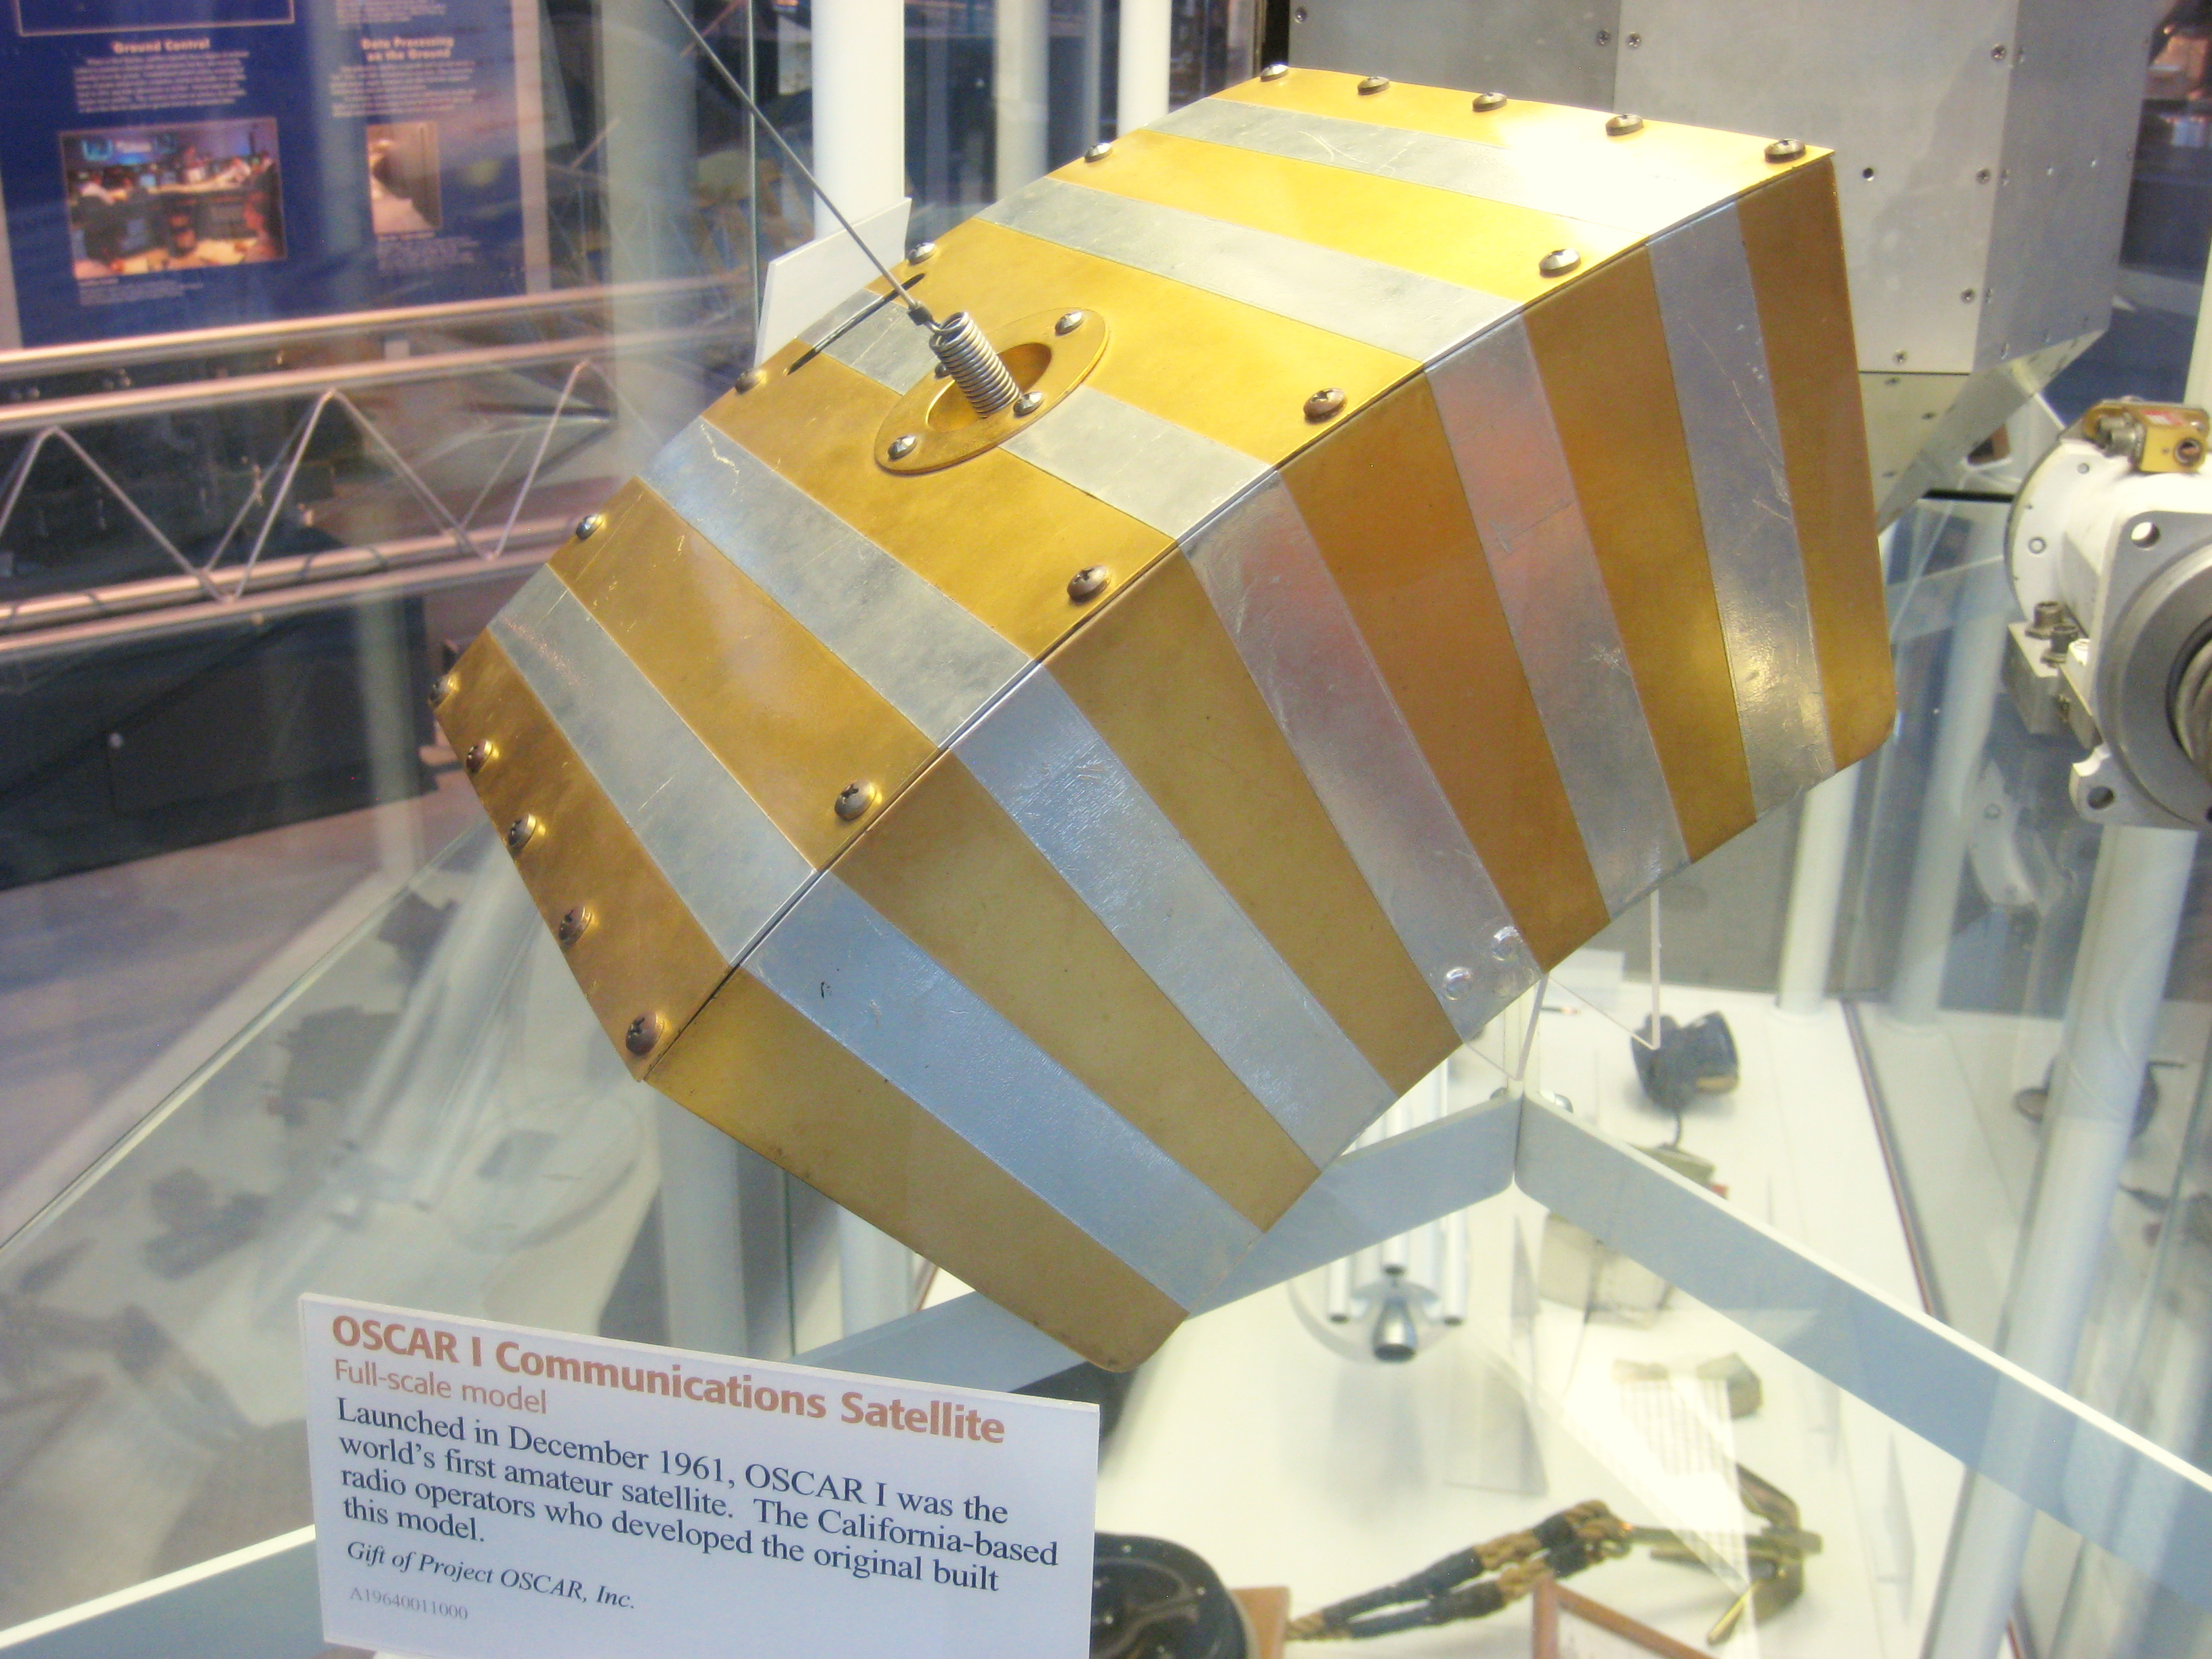
\includegraphics[width=0.85\textwidth]{foto/124}
    \caption{\scriptsize Modell des ersten Amateurfunksatelliten OSCAR 1, der 1961 für 22 Tage aus dem Orbit der Erde eine Bake im \qty{2}{\metre}-Band sendete und von 570 Funkamateuren aus 28 Ländern gehört wurde}
    \label{n_satellit_oscar1}
\end{figure}

    \end{column}
   \begin{column}{0.48\textwidth}
       \begin{itemize}
  \item Umrunden die Erde in kreis- oder elliptischen Bahnen und in unterschiedlichen Höhen
  \item Erster Amateurfunksatellit bereits 1961 (OSCAR 1)
  \item OSCAR: \enquote{Orbiting Satellite Carrying Amateur Radio}
  \item Bis heute mehrere 100 Satelliten im Orbit (gewesen)
  \end{itemize}

   \end{column}
\end{columns}

\end{frame}

\begin{frame}
\only<1>{
\begin{QQuestion}{BE415}{Wofür steht die Abkürzung OSCAR im Amateurfunk?}{Fahrzeug mit betriebsbereiter Amateurfunkstelle (Operational Station on a CAR)}
{Schiff auf See mit Amateurfunkstelle (Offshore Ship Carrying Amateur Radio)}
{Satellit mit Amateurfunkstelle (Orbiting Satellite Carrying Amateur Radio)}
{Amateurfunkstelle im Luftradarbetrieb (Observation Station Conducting Aeronautical Radar)}
\end{QQuestion}

}
\only<2>{
\begin{QQuestion}{BE415}{Wofür steht die Abkürzung OSCAR im Amateurfunk?}{Fahrzeug mit betriebsbereiter Amateurfunkstelle (Operational Station on a CAR)}
{Schiff auf See mit Amateurfunkstelle (Offshore Ship Carrying Amateur Radio)}
{\textbf{\textcolor{DARCgreen}{Satellit mit Amateurfunkstelle (Orbiting Satellite Carrying Amateur Radio)}}}
{Amateurfunkstelle im Luftradarbetrieb (Observation Station Conducting Aeronautical Radar)}
\end{QQuestion}

}
\end{frame}

\begin{frame}
\frametitle{Transponder}
Relaisfunkstelle auf dem Satellit wird \enquote{Transponder} genannt
\begin{columns}
    \begin{column}{0.48\textwidth}
    Uplink: Funkstrecke von der Erde zum Satelliten


    \end{column}
   \begin{column}{0.48\textwidth}
       Downlink: Funkstrecke vom Satelliten zur Erde


   \end{column}
\end{columns}

\begin{itemize}
  \item Unterschiedliche Frequenzbänder für Up- und Downlink
  \item Einfachere Trennung von Sende- und Empfangssignal
  \item Baugröße von Filtern wird reduziert
  \end{itemize}

\end{frame}

\begin{frame}
\only<1>{
\begin{QQuestion}{BE416}{Was versteht man unter dem Transponder eines \glqq OSCAR\grqq{} und wie arbeitet er?}{Dies ist ein Umsetzer an Bord eines Amateurfunksatelliten, der die aufgenommenen Signale in einen anderen Frequenzbereich umsetzt und wieder zur Erde sendet.}
{Es handelt sich um einen mit einer fernbedienten Amateurfunkstelle bestückten Stratosphärenballon, der empfangene Signale aufbereitet zur Erde zurücksendet.}
{Dies ist ein Umsetzer an Bord eines Amateurfunksatelliten, der die vom Satelliten aufgenommenen Wetterbilder und weitere Telemetriedaten automatisch zur Erde sendet.}
{Dies ist ein Bakensender an Bord eines Amateurfunksatelliten, der zur Beobachtung der Ausbreitungsbedingungen im VHF-, UHF- und SHF-Bereich dient.}
\end{QQuestion}

}
\only<2>{
\begin{QQuestion}{BE416}{Was versteht man unter dem Transponder eines \glqq OSCAR\grqq{} und wie arbeitet er?}{\textbf{\textcolor{DARCgreen}{Dies ist ein Umsetzer an Bord eines Amateurfunksatelliten, der die aufgenommenen Signale in einen anderen Frequenzbereich umsetzt und wieder zur Erde sendet.}}}
{Es handelt sich um einen mit einer fernbedienten Amateurfunkstelle bestückten Stratosphärenballon, der empfangene Signale aufbereitet zur Erde zurücksendet.}
{Dies ist ein Umsetzer an Bord eines Amateurfunksatelliten, der die vom Satelliten aufgenommenen Wetterbilder und weitere Telemetriedaten automatisch zur Erde sendet.}
{Dies ist ein Bakensender an Bord eines Amateurfunksatelliten, der zur Beobachtung der Ausbreitungsbedingungen im VHF-, UHF- und SHF-Bereich dient.}
\end{QQuestion}

}
\end{frame}

\begin{frame}
\only<1>{
\begin{QQuestion}{BE411}{Was bedeutet der Begriff Uplink im Bereich der Satellitenkommunikation?}{Senderichtung vom Satelliten zur Erde}
{Senderichtung von der Erde zum Satelliten}
{Horizontaler Winkel der Antenne}
{Vertikaler Winkel der Antenne}
\end{QQuestion}

}
\only<2>{
\begin{QQuestion}{BE411}{Was bedeutet der Begriff Uplink im Bereich der Satellitenkommunikation?}{Senderichtung vom Satelliten zur Erde}
{\textbf{\textcolor{DARCgreen}{Senderichtung von der Erde zum Satelliten}}}
{Horizontaler Winkel der Antenne}
{Vertikaler Winkel der Antenne}
\end{QQuestion}

}
\end{frame}

\begin{frame}
\only<1>{
\begin{QQuestion}{BE412}{Was bedeutet der Begriff Downlink im Bereich der Satellitenkommunikation?}{Senderichtung vom Satelliten zur Erde}
{Senderichtung von der Erde zum Satelliten}
{Horizontaler Winkel der Antenne}
{Vertikaler Winkel der Antenne}
\end{QQuestion}

}
\only<2>{
\begin{QQuestion}{BE412}{Was bedeutet der Begriff Downlink im Bereich der Satellitenkommunikation?}{\textbf{\textcolor{DARCgreen}{Senderichtung vom Satelliten zur Erde}}}
{Senderichtung von der Erde zum Satelliten}
{Horizontaler Winkel der Antenne}
{Vertikaler Winkel der Antenne}
\end{QQuestion}

}
\end{frame}

\begin{frame}
\only<1>{
\begin{QQuestion}{NF113}{Warum befinden sich bei Satellitenbetrieb Up- und Downlink in der Regel nicht im gleichen Frequenzband? Man benutzt unterschiedliche Frequenzbänder, weil~...}{der Uplink durch die Ionosphäre stärker bedämpft wird als der Downlink.}
{dies eine einfachere Trennung von Sende- und Empfangssignal ermöglicht und die Baugröße von Filtern auf dem Satelliten reduziert wird.}
{die Bandbreite auf beiden Frequenzbändern aufgeteilt wird und Bandbereiche besser ausgenutzt werden können. }
{man damit den Dopplereffekt vermindert.}
\end{QQuestion}

}
\only<2>{
\begin{QQuestion}{NF113}{Warum befinden sich bei Satellitenbetrieb Up- und Downlink in der Regel nicht im gleichen Frequenzband? Man benutzt unterschiedliche Frequenzbänder, weil~...}{der Uplink durch die Ionosphäre stärker bedämpft wird als der Downlink.}
{\textbf{\textcolor{DARCgreen}{dies eine einfachere Trennung von Sende- und Empfangssignal ermöglicht und die Baugröße von Filtern auf dem Satelliten reduziert wird.}}}
{die Bandbreite auf beiden Frequenzbändern aufgeteilt wird und Bandbereiche besser ausgenutzt werden können. }
{man damit den Dopplereffekt vermindert.}
\end{QQuestion}

}
\end{frame}

\begin{frame}
\frametitle{Azimut und Elevation}
Satellitenantennen müssen ausgerichtet sein
\begin{columns}
    \begin{column}{0.48\textwidth}
    Azimut

\begin{itemize}
  \item stammt von arabisch السموت (as-sumūt, \enquote{die Wege})
  \item Richtung entlang des Horizonts
  \item Wird wie beim Kompass in Grad gemessen
  \item \qty{0}{\degree}/\qty{360}{\degree} Norden – \qty{90}{\degree} Osten – \qty{180}{\degree} Süden – \qty{270}{\degree} Westen
  \end{itemize}

    \end{column}
   \begin{column}{0.48\textwidth}
       Elevation

\begin{itemize}
  \item leitet sich von lateinisch elevare (\enquote{erheben}) ab
  \item Vertikaler Winkel über dem Horizont
  \item \qty{0}{\degree} $\rightarrow$ direkt am Horizont
  \item \qty{90}{\degree} $\rightarrow$ senkrecht über einem
  \end{itemize}

   \end{column}
\end{columns}

\end{frame}

\begin{frame}
\only<1>{
\begin{QQuestion}{BE413}{Was bedeutet der Begriff Azimut im Bereich der Satellitenkommunikation?}{Vertikaler Winkel der Antenne}
{Horizontaler Winkel der Antenne}
{Senderichtung vom Satelliten zur Erde}
{Senderichtung von der Erde zum Satelliten}
\end{QQuestion}

}
\only<2>{
\begin{QQuestion}{BE413}{Was bedeutet der Begriff Azimut im Bereich der Satellitenkommunikation?}{Vertikaler Winkel der Antenne}
{\textbf{\textcolor{DARCgreen}{Horizontaler Winkel der Antenne}}}
{Senderichtung vom Satelliten zur Erde}
{Senderichtung von der Erde zum Satelliten}
\end{QQuestion}

}
\end{frame}

\begin{frame}
\only<1>{
\begin{QQuestion}{BE414}{Was bedeutet der Begriff Elevation im Bereich der Satellitenkommunikation?}{Horizontaler Winkel der Antenne}
{Vertikaler Winkel der Antenne}
{Senderichtung vom Satelliten zur Erde}
{Senderichtung von der Erde zum Satelliten}
\end{QQuestion}

}
\only<2>{
\begin{QQuestion}{BE414}{Was bedeutet der Begriff Elevation im Bereich der Satellitenkommunikation?}{Horizontaler Winkel der Antenne}
{\textbf{\textcolor{DARCgreen}{Vertikaler Winkel der Antenne}}}
{Senderichtung vom Satelliten zur Erde}
{Senderichtung von der Erde zum Satelliten}
\end{QQuestion}

}
\end{frame}

\begin{frame}
\frametitle{Steuersignale}
\begin{itemize}
  \item Im Amateurfunkdienst gibt es eine Pflicht zur offenen Sprache
  \item Ausnahme: Steuersignale zwischen Bodenstationen und Amateurfunksatelliten
  \item Dürfen zum Zwecke der Verschleierung verschlüsselt werden
  \item Damit können Dritte die Signale nicht mitlesen
  \item Dient der Sicherheit der Satelliten vor Steuerkommandos von Unbefugten
  \item In Deutschland gilt das auch für automatische und fernbediente Stationen sowie Remote-Stationen
  \end{itemize}
\end{frame}

\begin{frame}
\only<1>{
\begin{QQuestion}{VA303}{Welche Kommunikationsinhalte dürfen im internationalen Amateurfunkverkehr laut Radio Regulations (RR) zum Zwecke der Verschleierung verschlüsselt werden?}{Vertrauliche Informationen und Mitteilungen persönlicher Art}
{Steuersignale zwischen Bodenkontrollstationen auf der Erde und Amateurfunksatelliten}
{Inhalte, die auf Grund des verwendeten Übertragungsverfahrens digital codiert werden}
{Inhalte, die schützenswerte technische Sachverhalte des Amateurfunkdienstes betreffen}
\end{QQuestion}

}
\only<2>{
\begin{QQuestion}{VA303}{Welche Kommunikationsinhalte dürfen im internationalen Amateurfunkverkehr laut Radio Regulations (RR) zum Zwecke der Verschleierung verschlüsselt werden?}{Vertrauliche Informationen und Mitteilungen persönlicher Art}
{\textbf{\textcolor{DARCgreen}{Steuersignale zwischen Bodenkontrollstationen auf der Erde und Amateurfunksatelliten}}}
{Inhalte, die auf Grund des verwendeten Übertragungsverfahrens digital codiert werden}
{Inhalte, die schützenswerte technische Sachverhalte des Amateurfunkdienstes betreffen}
\end{QQuestion}

}
\end{frame}

\begin{frame}
\only<1>{
\begin{QQuestion}{VD104}{Welche Kommunikationsinhalte dürfen im Amateurfunkverkehr laut AFuV zum Zwecke der Verschleierung verschlüsselt werden?}{Inhalte, die auf Grund des verwendeten Übertragungsverfahrens digital codiert werden}
{Steuersignale für Satelliten, vertrauliche Informationen und Mitteilung persönlicher Art}
{Steuersignale für Satelliten, für fernbediente und automatisch arbeitende Stationen und für Remote-Betrieb}
{Inhalte, die schützenswerte technische Sachverhalte des Amateurfunkdienstes betreffen}
\end{QQuestion}

}
\only<2>{
\begin{QQuestion}{VD104}{Welche Kommunikationsinhalte dürfen im Amateurfunkverkehr laut AFuV zum Zwecke der Verschleierung verschlüsselt werden?}{Inhalte, die auf Grund des verwendeten Übertragungsverfahrens digital codiert werden}
{Steuersignale für Satelliten, vertrauliche Informationen und Mitteilung persönlicher Art}
{\textbf{\textcolor{DARCgreen}{Steuersignale für Satelliten, für fernbediente und automatisch arbeitende Stationen und für Remote-Betrieb}}}
{Inhalte, die schützenswerte technische Sachverhalte des Amateurfunkdienstes betreffen}
\end{QQuestion}

}
\end{frame}%ENDCONTENT


\section{Exterritoriale Stationen}
\label{section:exterritoriale_stationen}
\begin{frame}%STARTCONTENT

\begin{columns}
    \begin{column}{0.48\textwidth}
    \begin{itemize}
  \item Amateurfunkstelle außerhalb des Hoheitsgebiets der BRD
  \item Und kein anderes Land hat an diesem Standort ein Hoheitsgebiet
  \item Rufzeichen aus dem Block DP0AA bis DP2ZZ
  \end{itemize}

    \end{column}
   \begin{column}{0.48\textwidth}
       
\begin{figure}
    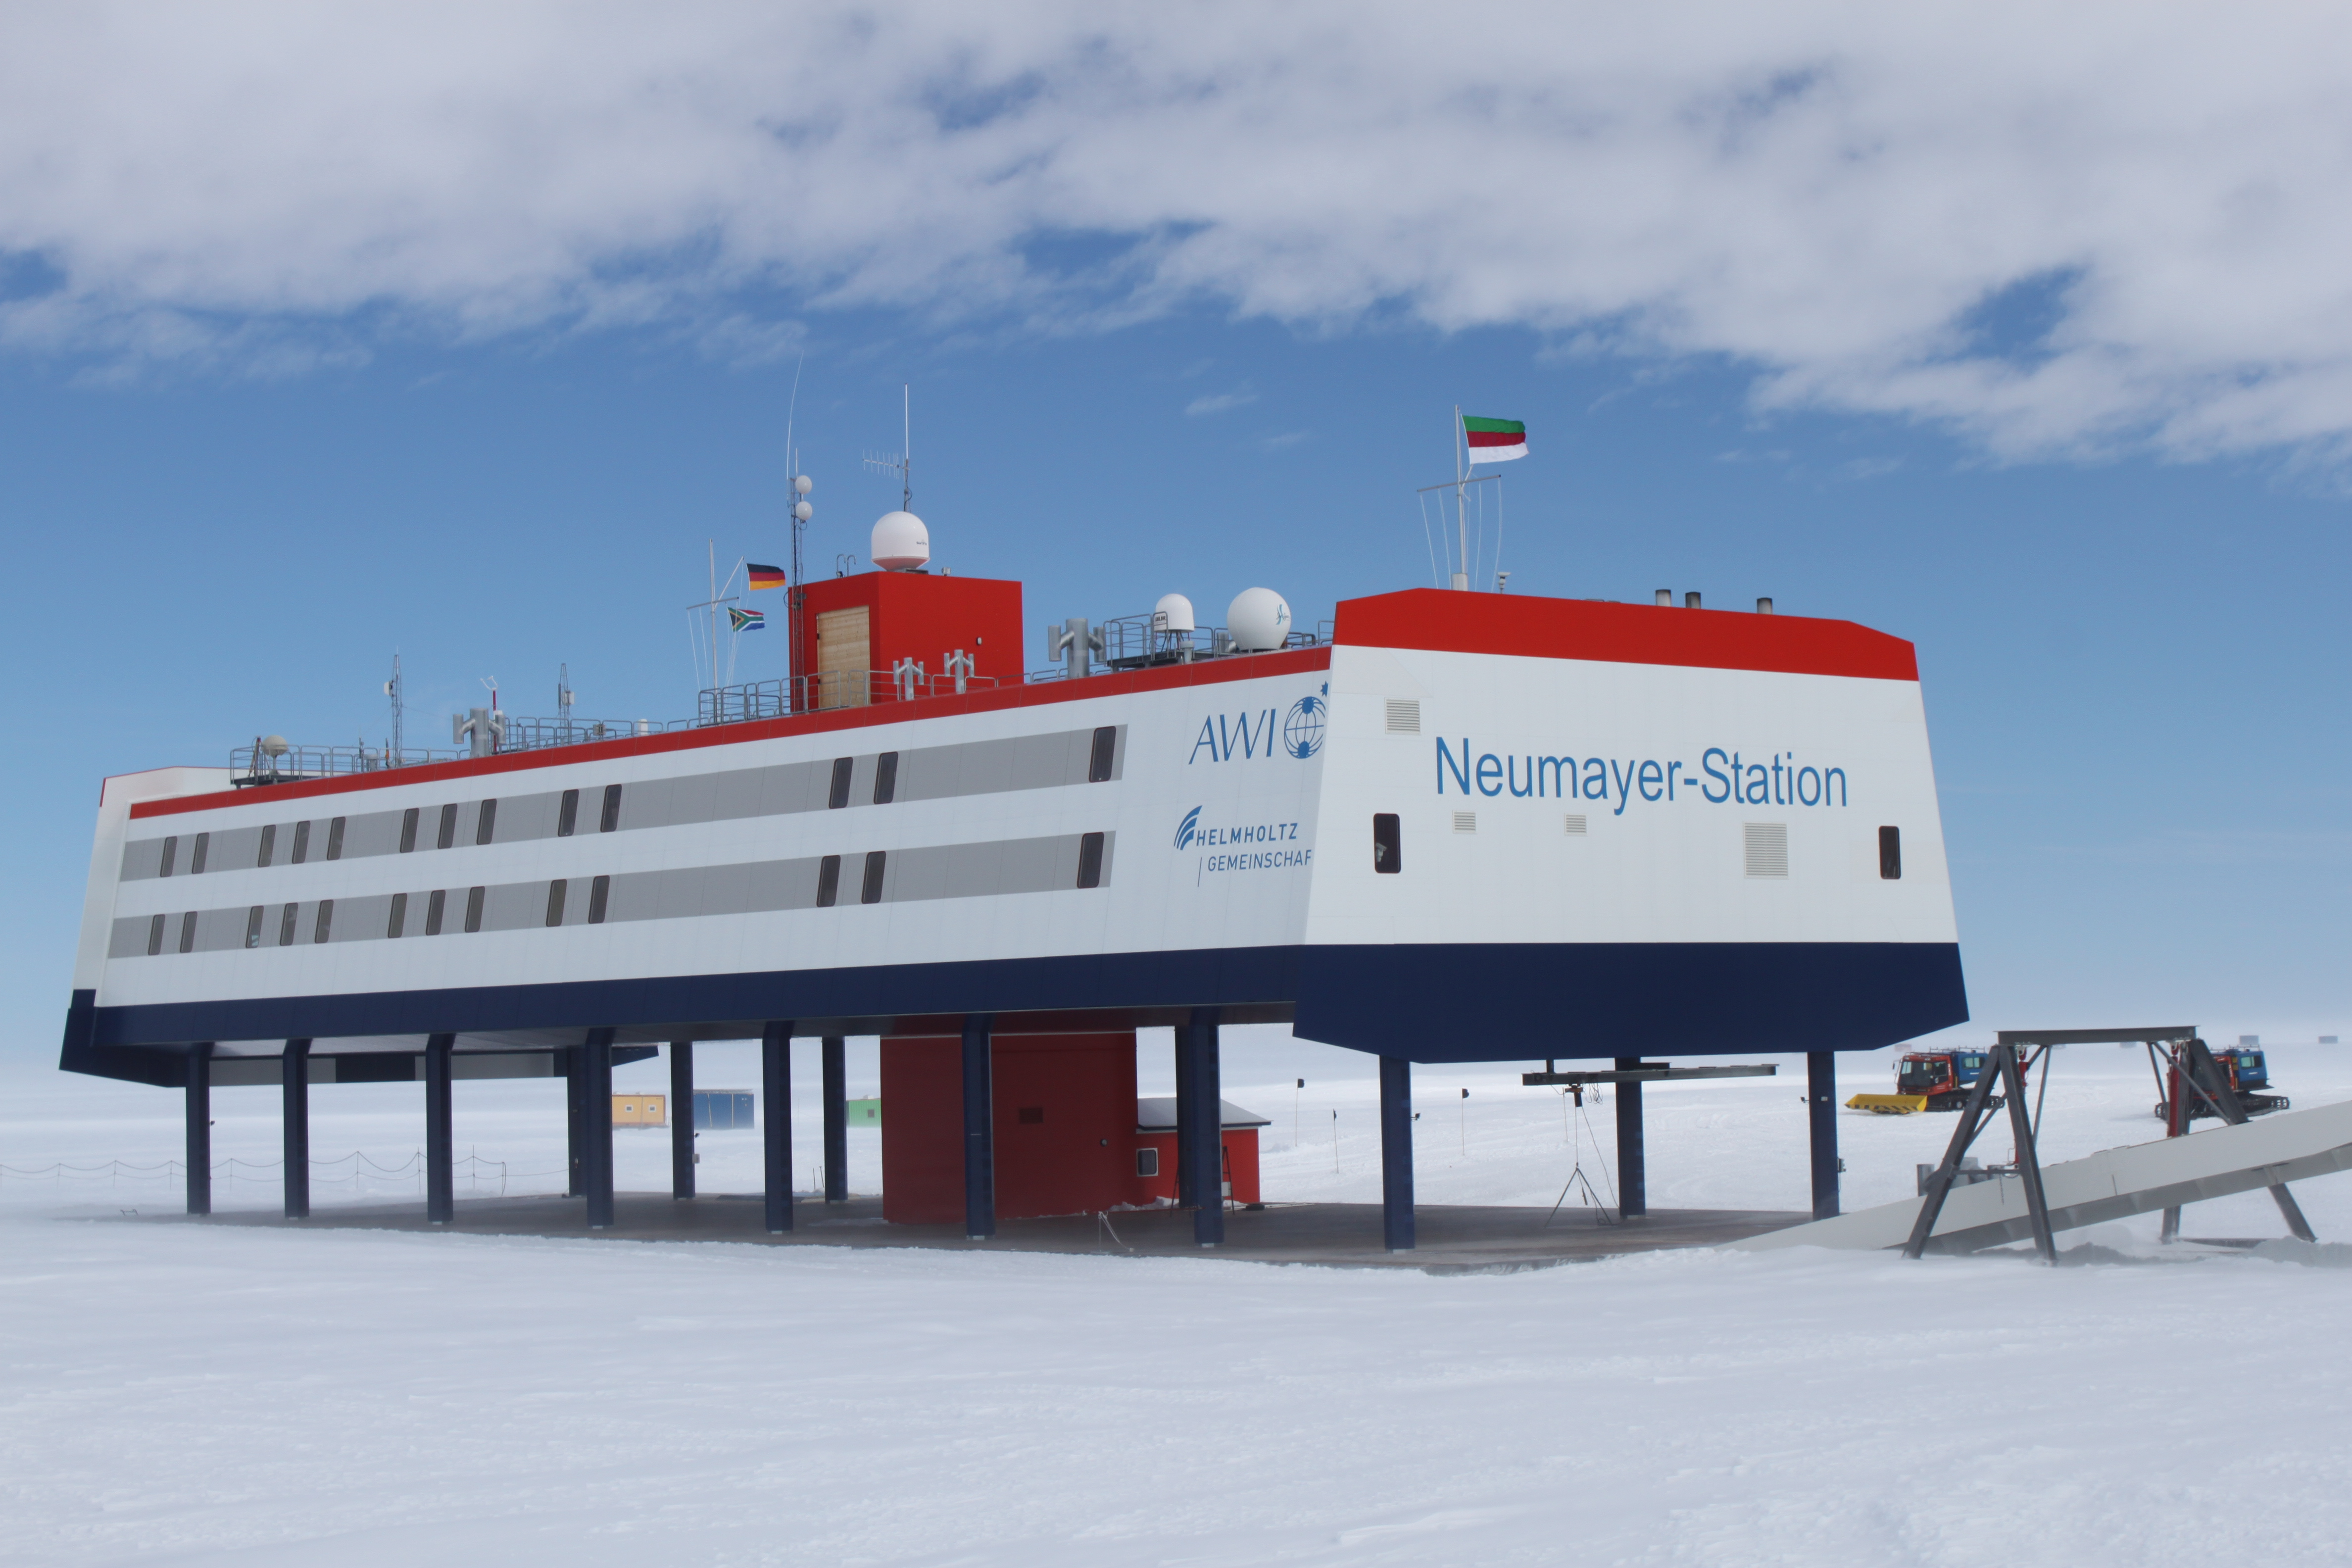
\includegraphics[width=0.85\textwidth]{foto/126}
    \caption{\scriptsize Auf der Polarforschungsstation Neumayer III befindet sich die Amateurfunkstation DP0GVN.}
    \label{n_exterritoriale_stationen_neumeyer_station}
\end{figure}

   \end{column}
\end{columns}

\end{frame}

\begin{frame}
\begin{columns}
    \begin{column}{0.48\textwidth}
    Beispiele:

\begin{itemize}
  \item Internationale Raumstation (ISS): DP0ISS
  \item Neumayer~III-Forschungsstation in der Antarktis: DP0GVN
  \item Forschungsschiff Polarstern: DP0POL
  \end{itemize}

    \end{column}
   \begin{column}{0.48\textwidth}
       
\begin{figure}
    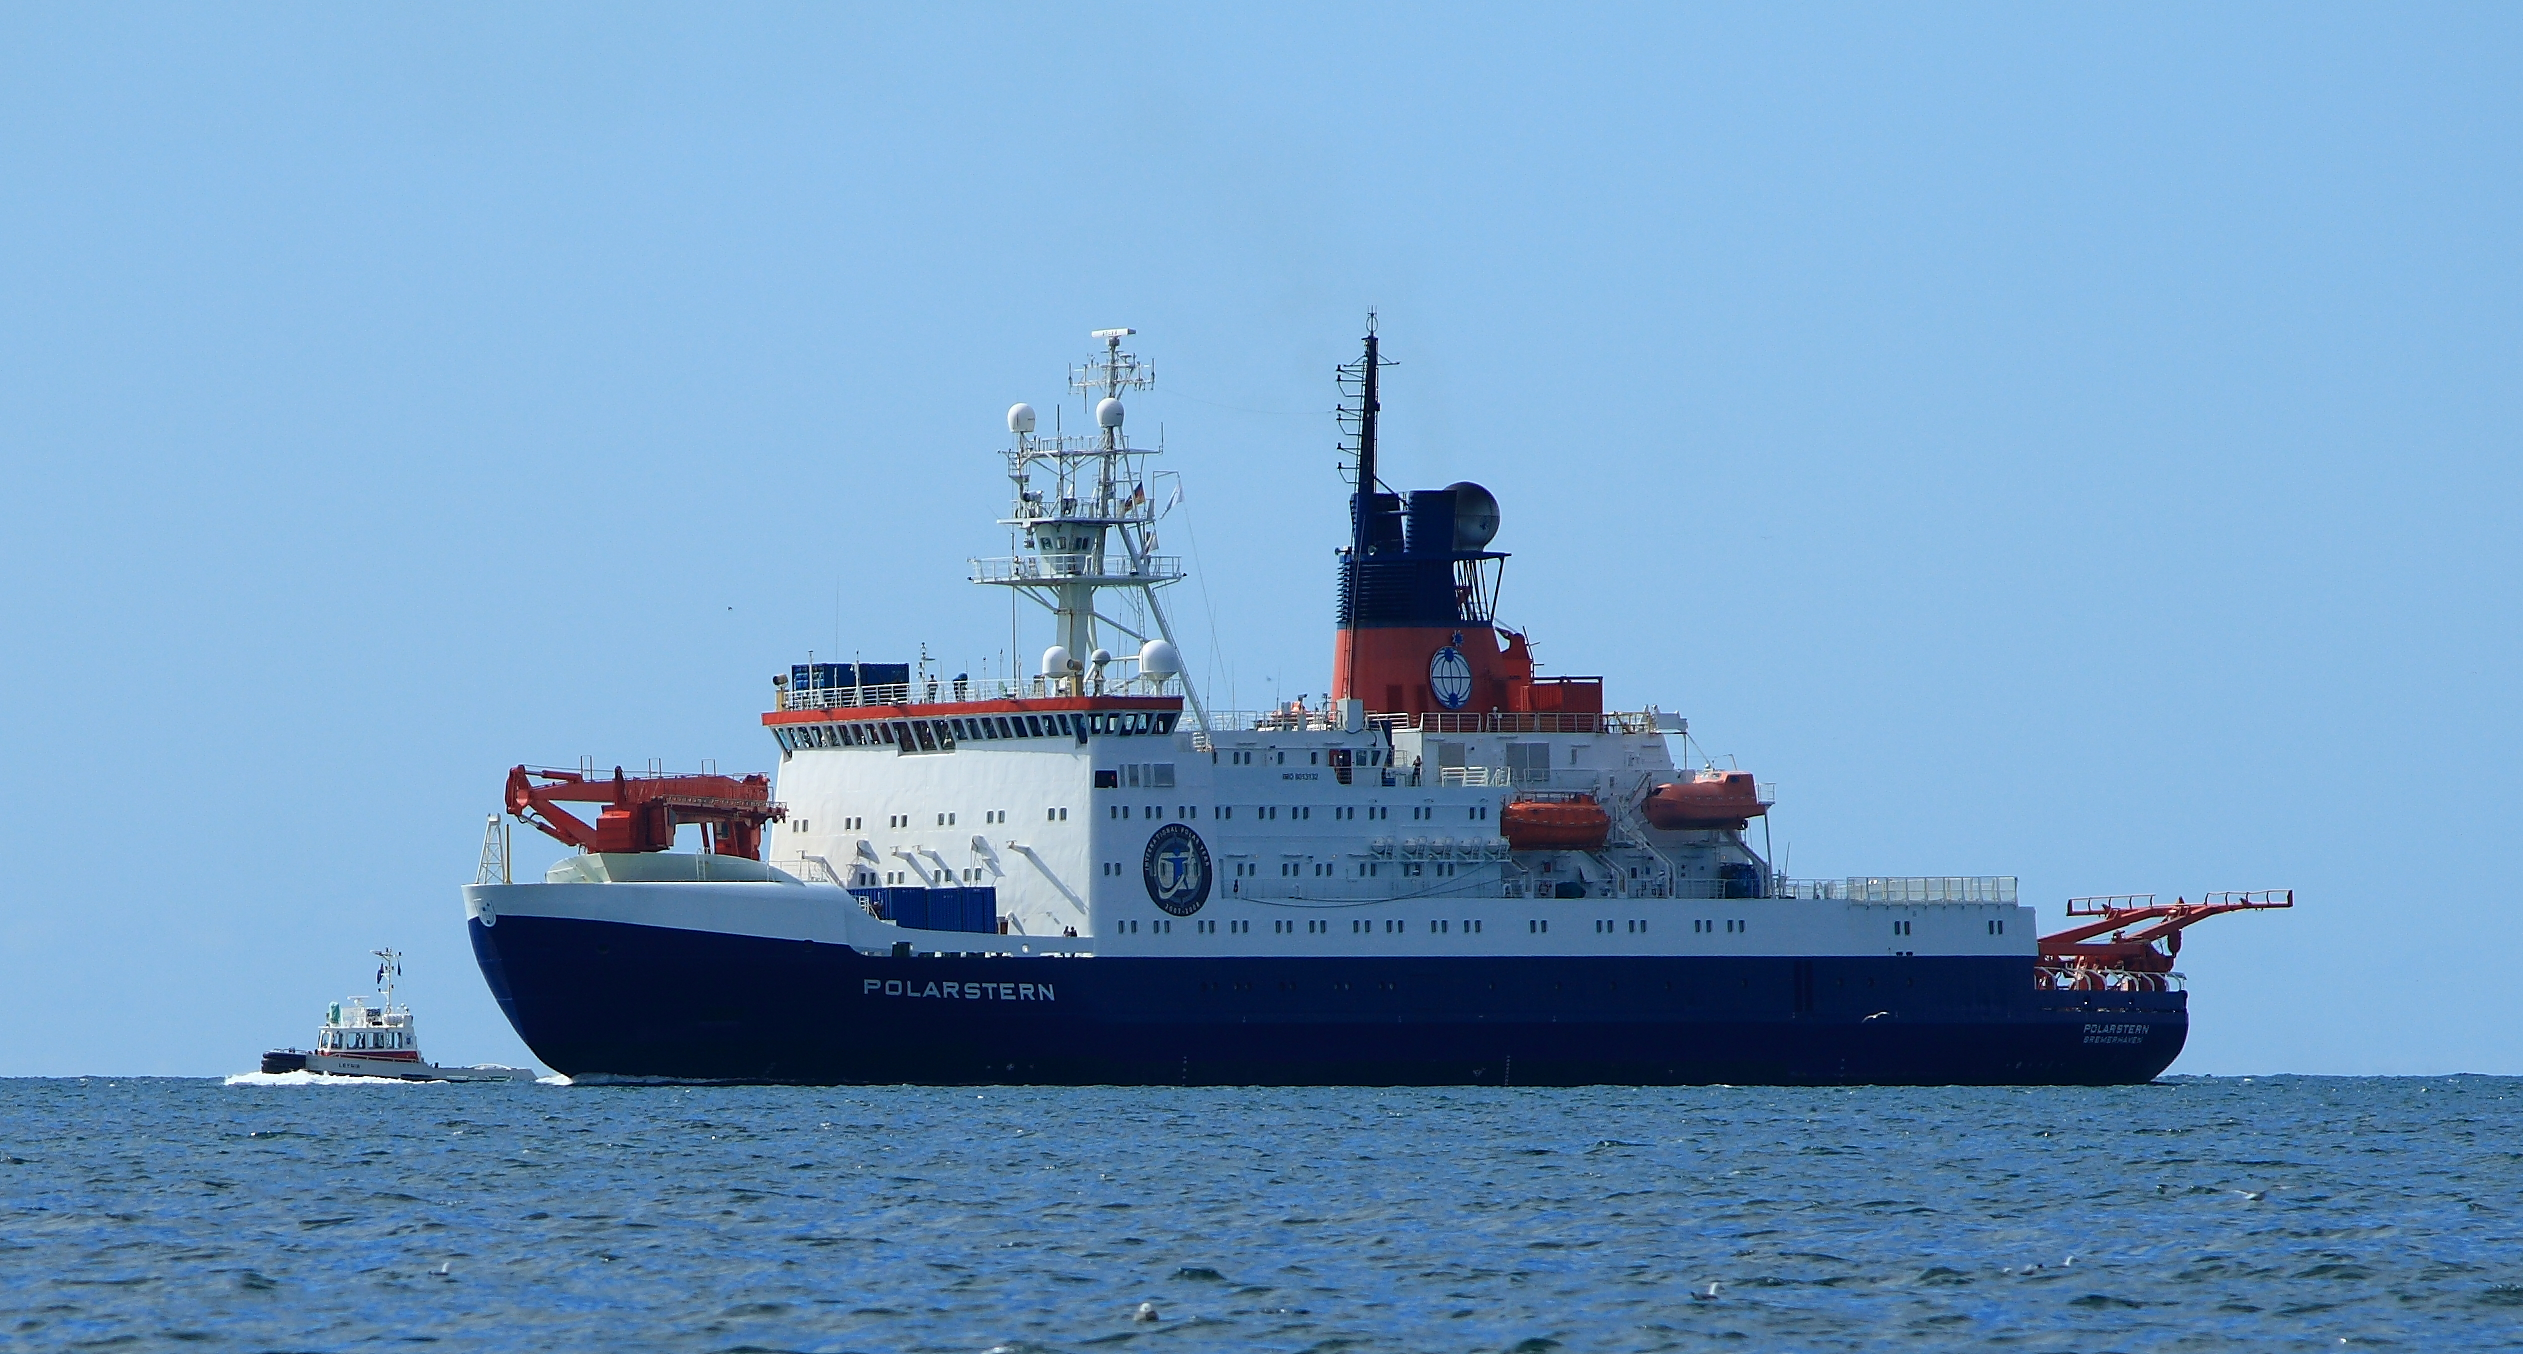
\includegraphics[width=0.85\textwidth]{foto/125}
    \caption{\scriptsize Die Amateurfunkstation an Bord des Forschungsschiff Polarstern verwendet das Rufzeichen DP0POL.}
    \label{n_exterritoriale_stationen_polarstern}
\end{figure}

   \end{column}
\end{columns}

\end{frame}

\begin{frame}
\only<1>{
\begin{QQuestion}{BD107}{Sie hören die Station DP0GVN. Um welche Art von Amateurfunkstelle handelt es sich? Es handelt sich um eine~...}{Amateurfunkstelle der Klasse A, die exterritorial betrieben wird.}
{Amateurfunkstelle der Klasse E, die ohne Anzeige nach BEMFV betrieben werden darf.}
{Klubstation der Klasse A von Funkamateuren, die Angehörige der Gaststreitkräfte in Deutschland sind.}
{Amateurfunkstelle der Klasse E, die exterritorial betrieben wird.}
\end{QQuestion}

}
\only<2>{
\begin{QQuestion}{BD107}{Sie hören die Station DP0GVN. Um welche Art von Amateurfunkstelle handelt es sich? Es handelt sich um eine~...}{\textbf{\textcolor{DARCgreen}{Amateurfunkstelle der Klasse A, die exterritorial betrieben wird.}}}
{Amateurfunkstelle der Klasse E, die ohne Anzeige nach BEMFV betrieben werden darf.}
{Klubstation der Klasse A von Funkamateuren, die Angehörige der Gaststreitkräfte in Deutschland sind.}
{Amateurfunkstelle der Klasse E, die exterritorial betrieben wird.}
\end{QQuestion}

}
\end{frame}

\begin{frame}
\only<1>{
\begin{QQuestion}{BD108}{Sie hören die Station DP0POL. Um welche Art von Amateurfunkstelle handelt es sich? Es handelt sich um eine Amateurfunkstelle~...}{von Angehörigen der Gaststreitkräfte in Deutschland.}
{der Klasse E, die ohne Anzeige nach BEMFV betrieben werden darf.}
{eines ausländischen Funkamateurs, der eine Amateurfunkprüfungsbescheinigung, aber kein individuelles Rufzeichen hat.}
{der Klasse A, die an einem exterritorialen Standort betrieben wird.}
\end{QQuestion}

}
\only<2>{
\begin{QQuestion}{BD108}{Sie hören die Station DP0POL. Um welche Art von Amateurfunkstelle handelt es sich? Es handelt sich um eine Amateurfunkstelle~...}{von Angehörigen der Gaststreitkräfte in Deutschland.}
{der Klasse E, die ohne Anzeige nach BEMFV betrieben werden darf.}
{eines ausländischen Funkamateurs, der eine Amateurfunkprüfungsbescheinigung, aber kein individuelles Rufzeichen hat.}
{\textbf{\textcolor{DARCgreen}{der Klasse A, die an einem exterritorialen Standort betrieben wird.}}}
\end{QQuestion}

}
\end{frame}%ENDCONTENT


\section{Experimentelle Studien}
\label{section:experimentelle_studien}
\begin{frame}%STARTCONTENT
\begin{itemize}
  \item Für besondere experimentelle und technisch-wissenschaftliche Studien
  \item Zeitlich und im Berechtigungsumfang eingeschränkt
  \item Werden gemäß §~16 Absatz 2 Satz 2 AFuV betrieben
  \item Klasse~A: DA5AA bis DA5ZZZ
  \item Klasse~E: DA4AA bis DA4ZZZ
  \item Bei der BNetzA zu beantragen
  \end{itemize}
\end{frame}

\begin{frame}
\only<1>{
\begin{QQuestion}{BD102}{Sie hören die Station DA5XX. Um welche Art von Amateurfunkstelle handelt es sich? Es handelt sich um eine~...}{Kurzzeitzuteilung für einen ausländischen Funkamateur, der eine Amateurfunkprüfungsbescheinigung, aber kein individuelles Rufzeichen hat.}
{Versuchsfunkstelle, die zur Erprobung technischer oder wissenschaftlicher Entwicklungen betrieben wird.}
{exterritoriale deutsche Funkstelle des Amateurfunkdienstes oder des Amateurfunkdienstes über Satelliten.}
{Amateurfunkstelle, die für besondere experimentelle Studien gemäß § 16 Absatz 2 AFuV betrieben wird.}
\end{QQuestion}

}
\only<2>{
\begin{QQuestion}{BD102}{Sie hören die Station DA5XX. Um welche Art von Amateurfunkstelle handelt es sich? Es handelt sich um eine~...}{Kurzzeitzuteilung für einen ausländischen Funkamateur, der eine Amateurfunkprüfungsbescheinigung, aber kein individuelles Rufzeichen hat.}
{Versuchsfunkstelle, die zur Erprobung technischer oder wissenschaftlicher Entwicklungen betrieben wird.}
{exterritoriale deutsche Funkstelle des Amateurfunkdienstes oder des Amateurfunkdienstes über Satelliten.}
{\textbf{\textcolor{DARCgreen}{Amateurfunkstelle, die für besondere experimentelle Studien gemäß § 16 Absatz 2 AFuV betrieben wird.}}}
\end{QQuestion}

}
\end{frame}

\begin{frame}
\only<1>{
\begin{QQuestion}{VD116}{Für welche Zwecke sind Zuteilungen mit Ausnahmen von den technischen und betrieblichen Rahmenbedingungen der Amateurfunkverordnung (AFuV) möglich?}{Für Abgleicharbeiten und Messungen an Sendern ohne Abschlusswiderstand}
{Für Übungen zur Abwicklung des Funkverkehrs in Not- und Katastrophenfällen}
{Für besondere experimentelle und technisch-wissenschaftliche Studien mit einer Amateurfunkstelle}
{Für die Nutzung zusätzlicher Frequenzbereiche, die nicht im Frequenznutzungsplan für den Amateurfunkdienst ausgewiesen sind}
\end{QQuestion}

}
\only<2>{
\begin{QQuestion}{VD116}{Für welche Zwecke sind Zuteilungen mit Ausnahmen von den technischen und betrieblichen Rahmenbedingungen der Amateurfunkverordnung (AFuV) möglich?}{Für Abgleicharbeiten und Messungen an Sendern ohne Abschlusswiderstand}
{Für Übungen zur Abwicklung des Funkverkehrs in Not- und Katastrophenfällen}
{\textbf{\textcolor{DARCgreen}{Für besondere experimentelle und technisch-wissenschaftliche Studien mit einer Amateurfunkstelle}}}
{Für die Nutzung zusätzlicher Frequenzbereiche, die nicht im Frequenznutzungsplan für den Amateurfunkdienst ausgewiesen sind}
\end{QQuestion}

}
\end{frame}%ENDCONTENT


\title{DARC Amateurfunklehrgang Klasse NEA}
\author{Internationaler Funkbetrieb}
\institute{Deutscher Amateur Radio Club e.\,V.}
\begin{frame}
\maketitle
\end{frame}

\section{Internationale Landeskenner}
\label{section:internationale_landeskenner}
\begin{frame}%STARTCONTENT

\begin{columns}
    \begin{column}{0.48\textwidth}
    \begin{itemize}
  \item Anhand des Präfixes kann man erkennen, aus welchem Land ein Funkpartner kommt
  \item Blau markierte Länder kommen im Fragenkatalog vor
  \end{itemize}

    \end{column}
   \begin{column}{0.48\textwidth}
       
\begin{figure}
    \DARCimage{0.85\linewidth}{656include}
    \caption{\scriptsize Landeskenner in Europa}
    \label{n_internationale_landeskenner_eu}
\end{figure}


   \end{column}
\end{columns}

\end{frame}

\begin{frame}
\only<1>{
\begin{QQuestion}{BD301}{Wo können Sie nachschlagen, in welchem Land sich eine Amateurfunkstelle mit einem Ihnen bislang unbekannten Landeskenner befindet?}{In den Empfehlungen der IARU.}
{In der Rufzeichenliste der Bundesnetzagentur.}
{In der Landeskennerliste der ITU, Amateurfunkhandbüchern und Rufzeichenlisten.}
{Im Frequenzbereichszuweisungsplan der Bundesrepublik Deutschland.}
\end{QQuestion}

}
\only<2>{
\begin{QQuestion}{BD301}{Wo können Sie nachschlagen, in welchem Land sich eine Amateurfunkstelle mit einem Ihnen bislang unbekannten Landeskenner befindet?}{In den Empfehlungen der IARU.}
{In der Rufzeichenliste der Bundesnetzagentur.}
{\textbf{\textcolor{DARCgreen}{In der Landeskennerliste der ITU, Amateurfunkhandbüchern und Rufzeichenlisten.}}}
{Im Frequenzbereichszuweisungsplan der Bundesrepublik Deutschland.}
\end{QQuestion}

}
\end{frame}

\begin{frame}
\only<1>{
\begin{QQuestion}{BD314}{Welche Antwort enthält nur Landeskenner von Ländern, die an die Bundesrepublik Deutschland grenzen?}{SM, LA, LZ, HB0}
{EA, GM, OE, ON}
{F, HB9, OZ, SP}
{CT, I, LX, OK}
\end{QQuestion}

}
\only<2>{
\begin{QQuestion}{BD314}{Welche Antwort enthält nur Landeskenner von Ländern, die an die Bundesrepublik Deutschland grenzen?}{SM, LA, LZ, HB0}
{EA, GM, OE, ON}
{\textbf{\textcolor{DARCgreen}{F, HB9, OZ, SP}}}
{CT, I, LX, OK}
\end{QQuestion}

}
\end{frame}

\begin{frame}
\only<1>{
\begin{QQuestion}{BD311}{Welche Gruppe gibt die Landeskenner der Länder Spanien, Luxemburg und Polen für ihre Amateurfunkstellen richtig wieder?}{EI, LA, SM}
{EU, LZ, S0}
{EA, LX, SP}
{EM, LU, 4X}
\end{QQuestion}

}
\only<2>{
\begin{QQuestion}{BD311}{Welche Gruppe gibt die Landeskenner der Länder Spanien, Luxemburg und Polen für ihre Amateurfunkstellen richtig wieder?}{EI, LA, SM}
{EU, LZ, S0}
{\textbf{\textcolor{DARCgreen}{EA, LX, SP}}}
{EM, LU, 4X}
\end{QQuestion}

}
\end{frame}

\begin{frame}
\only<1>{
\begin{QQuestion}{BD304}{Welche Landeskenner sind der Reihe nach den folgenden Ländern zugeordnet? Die Landeskenner OE, PA, und SM entsprechen den Ländern~...}{Österreich, Niederlande und Schweden.}
{Österreich, Brasilien und Schweiz.}
{Österreich, Polen und Südafrika.}
{Österreich, Niederlande und Schottland.}
\end{QQuestion}

}
\only<2>{
\begin{QQuestion}{BD304}{Welche Landeskenner sind der Reihe nach den folgenden Ländern zugeordnet? Die Landeskenner OE, PA, und SM entsprechen den Ländern~...}{\textbf{\textcolor{DARCgreen}{Österreich, Niederlande und Schweden.}}}
{Österreich, Brasilien und Schweiz.}
{Österreich, Polen und Südafrika.}
{Österreich, Niederlande und Schottland.}
\end{QQuestion}

}
\end{frame}

\begin{frame}
\only<1>{
\begin{QQuestion}{BD307}{Welche Länder (Gebiete) sind der Reihe nach den folgenden Landeskennern zugeordnet? Die Landeskenner 4X, F und OZ entsprechen den Ländern (Gebieten)~...}{Israel, Frankreich und Dänemark.}
{Italien, Belgien und Slowakei.}
{Schweden, Belgien und Schottland.}
{Schweiz, Luxemburg und Polen.}
\end{QQuestion}

}
\only<2>{
\begin{QQuestion}{BD307}{Welche Länder (Gebiete) sind der Reihe nach den folgenden Landeskennern zugeordnet? Die Landeskenner 4X, F und OZ entsprechen den Ländern (Gebieten)~...}{\textbf{\textcolor{DARCgreen}{Israel, Frankreich und Dänemark.}}}
{Italien, Belgien und Slowakei.}
{Schweden, Belgien und Schottland.}
{Schweiz, Luxemburg und Polen.}
\end{QQuestion}

}
\end{frame}

\begin{frame}
\only<1>{
\begin{QQuestion}{BD303}{Welche Länder sind der Reihe nach den folgenden Landeskennern zugeordnet? Die Landeskenner OE, ON und OK entsprechen den Ländern~...}{Finnland, Tschechien und Dänemark.}
{Dänemark, Belgien und Slowakei.}
{Österreich, Dänemark und Belgien.}
{Österreich, Belgien und Tschechien.}
\end{QQuestion}

}
\only<2>{
\begin{QQuestion}{BD303}{Welche Länder sind der Reihe nach den folgenden Landeskennern zugeordnet? Die Landeskenner OE, ON und OK entsprechen den Ländern~...}{Finnland, Tschechien und Dänemark.}
{Dänemark, Belgien und Slowakei.}
{Österreich, Dänemark und Belgien.}
{\textbf{\textcolor{DARCgreen}{Österreich, Belgien und Tschechien.}}}
\end{QQuestion}

}
\end{frame}

\begin{frame}
\only<1>{
\begin{QQuestion}{BD305}{Welche Länder sind der Reihe nach den folgenden Landeskennern zugeordnet? Die Landeskenner F, PA und SP entsprechen den Ländern~...}{Frankreich, Niederlande und Polen.}
{Schweden, Niederlande und Polen.}
{Niederlande, Polen und Belgien.}
{Südafrika, Dänemark und Luxemburg.}
\end{QQuestion}

}
\only<2>{
\begin{QQuestion}{BD305}{Welche Länder sind der Reihe nach den folgenden Landeskennern zugeordnet? Die Landeskenner F, PA und SP entsprechen den Ländern~...}{\textbf{\textcolor{DARCgreen}{Frankreich, Niederlande und Polen.}}}
{Schweden, Niederlande und Polen.}
{Niederlande, Polen und Belgien.}
{Südafrika, Dänemark und Luxemburg.}
\end{QQuestion}

}
\end{frame}

\begin{frame}
\only<1>{
\begin{QQuestion}{BD306}{Welche Länder sind der Reihe nach den folgenden Landeskennern zugeordnet? Die Landeskenner SM, SP und ZS entsprechen den Ländern~...}{Schweden, Slowenien und Polen.}
{Schweden, Slowakei und Polen.}
{Slowenien, Polen und Schweden.}
{Schweden, Polen und Südafrika.}
\end{QQuestion}

}
\only<2>{
\begin{QQuestion}{BD306}{Welche Länder sind der Reihe nach den folgenden Landeskennern zugeordnet? Die Landeskenner SM, SP und ZS entsprechen den Ländern~...}{Schweden, Slowenien und Polen.}
{Schweden, Slowakei und Polen.}
{Slowenien, Polen und Schweden.}
{\textbf{\textcolor{DARCgreen}{Schweden, Polen und Südafrika.}}}
\end{QQuestion}

}
\end{frame}

\begin{frame}
\only<1>{
\begin{QQuestion}{BD308}{Welche Länder sind der Reihe nach den folgenden Landeskennern zugeordnet? Die Landeskenner EA, EI, EK, EM, ES entsprechen den Ländern~...}{Spanien, Ukraine, Armenien, Estland, Irland}
{Spanien, Ukraine, Armenien, Irland, Estland}
{Spanien, Irland, Armenien, Estland, Ukraine}
{Spanien, Irland, Armenien, Ukraine, Estland}
\end{QQuestion}

}
\only<2>{
\begin{QQuestion}{BD308}{Welche Länder sind der Reihe nach den folgenden Landeskennern zugeordnet? Die Landeskenner EA, EI, EK, EM, ES entsprechen den Ländern~...}{Spanien, Ukraine, Armenien, Estland, Irland}
{Spanien, Ukraine, Armenien, Irland, Estland}
{Spanien, Irland, Armenien, Estland, Ukraine}
{\textbf{\textcolor{DARCgreen}{Spanien, Irland, Armenien, Ukraine, Estland}}}
\end{QQuestion}

}
\end{frame}

\begin{frame}
\only<1>{
\begin{QQuestion}{BD310}{Welche Gruppe gibt die Landeskenner der Länder Schweiz, Spanien und Belgien für ihre Amateurfunkstellen richtig wieder?}{SZ, SP und BE}
{HB9, EA und ON}
{SP, ON und EA}
{EA, SP und BE}
\end{QQuestion}

}
\only<2>{
\begin{QQuestion}{BD310}{Welche Gruppe gibt die Landeskenner der Länder Schweiz, Spanien und Belgien für ihre Amateurfunkstellen richtig wieder?}{SZ, SP und BE}
{\textbf{\textcolor{DARCgreen}{HB9, EA und ON}}}
{SP, ON und EA}
{EA, SP und BE}
\end{QQuestion}

}
\end{frame}

\begin{frame}
\only<1>{
\begin{QQuestion}{BD302}{Welchem Land bzw. welchen Ländern sind die Landeskenner DA bis DZ zugeordnet?}{Deutschland (DA-DO), Taiwan (DP-DT) und Philippinen (DU-DZ)}
{Ausschließlich Deutschland (DA-DZ)}
{Deutschland (DA-DT) und Philippinen (DU-DZ)}
{Deutschland (DA-DR), Südkorea (DS-DT) und Philippinen (DU-DZ)}
\end{QQuestion}

}
\only<2>{
\begin{QQuestion}{BD302}{Welchem Land bzw. welchen Ländern sind die Landeskenner DA bis DZ zugeordnet?}{Deutschland (DA-DO), Taiwan (DP-DT) und Philippinen (DU-DZ)}
{Ausschließlich Deutschland (DA-DZ)}
{Deutschland (DA-DT) und Philippinen (DU-DZ)}
{\textbf{\textcolor{DARCgreen}{Deutschland (DA-DR), Südkorea (DS-DT) und Philippinen (DU-DZ)}}}
\end{QQuestion}

}
\end{frame}

\begin{frame}
\only<1>{
\begin{QQuestion}{BD312}{Welche Gruppe gibt Landeskenner der Länder USA, Neuseeland und Argentinien für ihre Amateurfunkstellen richtig wieder?}{AL, CE und VE}
{K, ZS und A}
{N, LU und PY}
{W, ZL und LU}
\end{QQuestion}

}
\only<2>{
\begin{QQuestion}{BD312}{Welche Gruppe gibt Landeskenner der Länder USA, Neuseeland und Argentinien für ihre Amateurfunkstellen richtig wieder?}{AL, CE und VE}
{K, ZS und A}
{N, LU und PY}
{\textbf{\textcolor{DARCgreen}{W, ZL und LU}}}
\end{QQuestion}

}
\end{frame}

\begin{frame}
\only<1>{
\begin{QQuestion}{BD313}{Welche Gruppe gibt Landeskenner der Länder China, Kanada und Australien für ihre Amateurfunkstellen richtig wieder?}{JA, VE und VK}
{BY, JA und VK}
{BY, VE und VK}
{N, VE und VK}
\end{QQuestion}

}
\only<2>{
\begin{QQuestion}{BD313}{Welche Gruppe gibt Landeskenner der Länder China, Kanada und Australien für ihre Amateurfunkstellen richtig wieder?}{JA, VE und VK}
{BY, JA und VK}
{\textbf{\textcolor{DARCgreen}{BY, VE und VK}}}
{N, VE und VK}
\end{QQuestion}

}
\end{frame}

\begin{frame}
\only<1>{
\begin{QQuestion}{BD316}{Welche drei Landeskenner sind einem einzigen Kontinent zuzuordnen?}{N, XE und DS}
{K, VE und BY}
{W, VE und XE}
{XE, VE und JA}
\end{QQuestion}

}
\only<2>{
\begin{QQuestion}{BD316}{Welche drei Landeskenner sind einem einzigen Kontinent zuzuordnen?}{N, XE und DS}
{K, VE und BY}
{\textbf{\textcolor{DARCgreen}{W, VE und XE}}}
{XE, VE und JA}
\end{QQuestion}

}
\end{frame}

\begin{frame}
\only<1>{
\begin{QQuestion}{BD318}{Welche Landeskenner sind asiatischen Ländern zugewiesen?}{JA, VU und PY}
{VU, JA und K}
{BY, JA und VU}
{LU, DS und JA}
\end{QQuestion}

}
\only<2>{
\begin{QQuestion}{BD318}{Welche Landeskenner sind asiatischen Ländern zugewiesen?}{JA, VU und PY}
{VU, JA und K}
{\textbf{\textcolor{DARCgreen}{BY, JA und VU}}}
{LU, DS und JA}
\end{QQuestion}

}
\end{frame}

\begin{frame}
\only<1>{
\begin{QQuestion}{BD317}{Welche Landeskenner sind südamerikanischen Ländern zugewiesen?}{LU, CE und BY}
{PY, CE und LU}
{CE, LU und JA}
{PY, CE und VE}
\end{QQuestion}

}
\only<2>{
\begin{QQuestion}{BD317}{Welche Landeskenner sind südamerikanischen Ländern zugewiesen?}{LU, CE und BY}
{\textbf{\textcolor{DARCgreen}{PY, CE und LU}}}
{CE, LU und JA}
{PY, CE und VE}
\end{QQuestion}

}
\end{frame}

\begin{frame}
\only<1>{
\begin{QQuestion}{BD309}{Welche Länder sind der Reihe nach den folgenden Landeskennern zugeordnet? Die Landeskenner VE, VK und PY entsprechen den Ländern~...}{Kanada, Australien und Brasilien.}
{Kanada, Brasilien und USA.}
{USA, Australien und Brasilien.}
{Kanada, Australien und Japan.}
\end{QQuestion}

}
\only<2>{
\begin{QQuestion}{BD309}{Welche Länder sind der Reihe nach den folgenden Landeskennern zugeordnet? Die Landeskenner VE, VK und PY entsprechen den Ländern~...}{\textbf{\textcolor{DARCgreen}{Kanada, Australien und Brasilien.}}}
{Kanada, Brasilien und USA.}
{USA, Australien und Brasilien.}
{Kanada, Australien und Japan.}
\end{QQuestion}

}
\end{frame}

\begin{frame}
\only<1>{
\begin{QQuestion}{BD315}{Welche Antwort gibt ausschließlich Rufzeichen aus den Vereinigten Staaten (USA) wieder?}{K1TTT, KA7KLE und UA3RUS}
{W0FKK, N6CAL und VE5VK}
{US2ABC, AB0GC und W4EAX}
{K3LR, W3DZZ und K4EAX}
\end{QQuestion}

}
\only<2>{
\begin{QQuestion}{BD315}{Welche Antwort gibt ausschließlich Rufzeichen aus den Vereinigten Staaten (USA) wieder?}{K1TTT, KA7KLE und UA3RUS}
{W0FKK, N6CAL und VE5VK}
{US2ABC, AB0GC und W4EAX}
{\textbf{\textcolor{DARCgreen}{K3LR, W3DZZ und K4EAX}}}
\end{QQuestion}

}
\end{frame}%ENDCONTENT


\section{ITU-Regionen}
\label{section:itu_regionen}
\begin{frame}%STARTCONTENT

\begin{columns}
    \begin{column}{0.48\textwidth}
    
\begin{figure}
    \DARCimage{0.85\linewidth}{658include}
    \caption{\scriptsize Kartendarstellung der ITU-Regionen}
    \label{n_itu_regionen_karte}
\end{figure}


    \end{column}
   \begin{column}{0.48\textwidth}
       \begin{itemize}
  \item Weltweite Koordinierung von Funkfrequenzen getrennt nach 3 Regionen
  \item Durch ITU geregelt
  \item Nötig, um unterschiedliche Zuweisungen von Frequenzbereichen zu Funkdiensten vorzunehmen
  \end{itemize}

   \end{column}
\end{columns}

\end{frame}

\begin{frame}
\only<1>{
\begin{QQuestion}{VA402}{Nach den Radio Regulations (RR) ist die Welt für die Zuweisung von Frequenzbereichen an Funkdienste in Regionen aufgeteilt. Wie viele Regionen gibt es?}{Zwei}
{Fünf}
{Vier}
{Drei}
\end{QQuestion}

}
\only<2>{
\begin{QQuestion}{VA402}{Nach den Radio Regulations (RR) ist die Welt für die Zuweisung von Frequenzbereichen an Funkdienste in Regionen aufgeteilt. Wie viele Regionen gibt es?}{Zwei}
{Fünf}
{Vier}
{\textbf{\textcolor{DARCgreen}{Drei}}}
\end{QQuestion}

}
\end{frame}

\begin{frame}
\only<1>{
\begin{QQuestion}{VA401}{Weshalb wird in den Radio Regulations (RR) die Erde in verschiedene Regionen eingeteilt?}{Weil es sich um unterschiedliche Zeitzonen handelt und es so den Funkverkehr vereinfacht}
{Weil der Amateurfunkverkehr nur innerhalb einer Region zulässig ist}
{Um für die einzelnen Regionen Regelungen für Gastlizenzen einführen zu können}
{Um in den Regionen unterschiedliche Frequenzbereichszuweisungen für die Funkdienste vornehmen zu können}
\end{QQuestion}

}
\only<2>{
\begin{QQuestion}{VA401}{Weshalb wird in den Radio Regulations (RR) die Erde in verschiedene Regionen eingeteilt?}{Weil es sich um unterschiedliche Zeitzonen handelt und es so den Funkverkehr vereinfacht}
{Weil der Amateurfunkverkehr nur innerhalb einer Region zulässig ist}
{Um für die einzelnen Regionen Regelungen für Gastlizenzen einführen zu können}
{\textbf{\textcolor{DARCgreen}{Um in den Regionen unterschiedliche Frequenzbereichszuweisungen für die Funkdienste vornehmen zu können}}}
\end{QQuestion}

}
\end{frame}

\begin{frame}
\only<1>{
\begin{QQuestion}{VA403}{Zu welcher Region nach den Radio Regulations (RR) gehört Deutschland?}{Region 2}
{Region 1}
{Region 3}
{Region 4}
\end{QQuestion}

}
\only<2>{
\begin{QQuestion}{VA403}{Zu welcher Region nach den Radio Regulations (RR) gehört Deutschland?}{Region 2}
{\textbf{\textcolor{DARCgreen}{Region 1}}}
{Region 3}
{Region 4}
\end{QQuestion}

}
\end{frame}

\begin{frame}
\only<1>{
\begin{QQuestion}{VA404}{Zu welcher Region nach den Radio Regulations (RR) gehört Kanada?}{Region 3}
{Region 2}
{Region 4}
{Region 1}
\end{QQuestion}

}
\only<2>{
\begin{QQuestion}{VA404}{Zu welcher Region nach den Radio Regulations (RR) gehört Kanada?}{Region 3}
{\textbf{\textcolor{DARCgreen}{Region 2}}}
{Region 4}
{Region 1}
\end{QQuestion}

}
\end{frame}

\begin{frame}
\only<1>{
\begin{QQuestion}{VA405}{Zu welcher Region nach den Radio Regulations (RR) gehört Australien?}{Region 3}
{Region 1}
{Region 2}
{Region 4}
\end{QQuestion}

}
\only<2>{
\begin{QQuestion}{VA405}{Zu welcher Region nach den Radio Regulations (RR) gehört Australien?}{\textbf{\textcolor{DARCgreen}{Region 3}}}
{Region 1}
{Region 2}
{Region 4}
\end{QQuestion}

}
\end{frame}%ENDCONTENT


\section{DX}
\label{section:dx}
\begin{frame}%STARTCONTENT
\begin{itemize}
  \item Funkverbindung über große Entfernung
  \item DX $\rightarrow$ \enquote{long distance} (aus Morsetelegrafie)
  \item Unterscheidung zwischen Kurzwelle und UKW
  \end{itemize}
\end{frame}

\begin{frame}
\frametitle{DX Kurzwelle}
\begin{columns}
    \begin{column}{0.48\textwidth}
    \begin{itemize}
  \item Kontakt mit Funkamateuren von einem anderen Kontinent
  \item Funkamateure vom selben Kontinent sollten nicht antworten
  \end{itemize}

    \end{column}
   \begin{column}{0.48\textwidth}
       
    \pause\QSOown{CQ DX}



   \end{column}
\end{columns}

\end{frame}

\begin{frame}
\only<1>{
\begin{QQuestion}{BB103}{Was bedeutet die betriebliche Abkürzung DX?}{Kleine Entfernung }
{Große Entfernung }
{Auf dem indirektem Weg}
{Auf dem direktem Weg}
\end{QQuestion}

}
\only<2>{
\begin{QQuestion}{BB103}{Was bedeutet die betriebliche Abkürzung DX?}{Kleine Entfernung }
{\textbf{\textcolor{DARCgreen}{Große Entfernung }}}
{Auf dem indirektem Weg}
{Auf dem direktem Weg}
\end{QQuestion}

}
\end{frame}

\begin{frame}
\only<1>{
\begin{QQuestion}{BE114}{Was bedeutet der im \qty{20}{\m}-Band gesendete Anruf \glqq CQ DX CQ DX DE HB9AFN HB9AFN K\grqq{}? HB9AFN sucht eine Verbindung mit~...}{einem anderen Kontinent und sollte durch europäische Funkamateure nicht angerufen werden.}
{dem Inland und sollte durch ausländische Funkamateure nicht angerufen werden.}
{Stationen in über \qty{500}{\km} Entfernung und sollte durch Funkamateure aus einer geringeren Entfernung nicht angerufen werden.}
{philippinischen Funkamateuren (Präfix \glqq DX\grqq{}) und sollte durch Funkamateure anderer Länder nicht angerufen werden.}
\end{QQuestion}

}
\only<2>{
\begin{QQuestion}{BE114}{Was bedeutet der im \qty{20}{\m}-Band gesendete Anruf \glqq CQ DX CQ DX DE HB9AFN HB9AFN K\grqq{}? HB9AFN sucht eine Verbindung mit~...}{\textbf{\textcolor{DARCgreen}{einem anderen Kontinent und sollte durch europäische Funkamateure nicht angerufen werden.}}}
{dem Inland und sollte durch ausländische Funkamateure nicht angerufen werden.}
{Stationen in über \qty{500}{\km} Entfernung und sollte durch Funkamateure aus einer geringeren Entfernung nicht angerufen werden.}
{philippinischen Funkamateuren (Präfix \glqq DX\grqq{}) und sollte durch Funkamateure anderer Länder nicht angerufen werden.}
\end{QQuestion}

}

\end{frame}

\begin{frame}
\only<1>{
\begin{QQuestion}{BB105}{Eine Station ruft in der Nacht auf \qty{3790}{\kHz} \glqq CQ DX\grqq{}. Wer soll antworten? Nur Stationen~...}{Stationen von anderen Kontinenten}
{mit DX-Präfix}
{im Nahbereich bis \qty{50}{\km} Entfernung}
{aus Deutschland}
\end{QQuestion}

}
\only<2>{
\begin{QQuestion}{BB105}{Eine Station ruft in der Nacht auf \qty{3790}{\kHz} \glqq CQ DX\grqq{}. Wer soll antworten? Nur Stationen~...}{\textbf{\textcolor{DARCgreen}{Stationen von anderen Kontinenten}}}
{mit DX-Präfix}
{im Nahbereich bis \qty{50}{\km} Entfernung}
{aus Deutschland}
\end{QQuestion}

}

\end{frame}

\begin{frame}
\frametitle{DX auf VHF/UHF}
\begin{itemize}
  \item Andere Kontinente erreicht man darüber nur sehr selten
  \item Deshalb Funkkontakte in erkennbar einigen hundert Kilometern Entfernung
  \end{itemize}

\end{frame}

\begin{frame}
\only<1>{
\begin{QQuestion}{BB104}{Eine Station ruft auf VHF/UHF \glqq CQ DX\grqq{}. Wer soll antworten?}{Stationen von anderen Kontinenten}
{Stationen auf den Philippinen}
{Stationen in mehr als einigen \qty{100}{\km} Entfernung}
{Stationen mit deutschem Präfix}
\end{QQuestion}

}
\only<2>{
\begin{QQuestion}{BB104}{Eine Station ruft auf VHF/UHF \glqq CQ DX\grqq{}. Wer soll antworten?}{Stationen von anderen Kontinenten}
{Stationen auf den Philippinen}
{\textbf{\textcolor{DARCgreen}{Stationen in mehr als einigen \qty{100}{\km} Entfernung}}}
{Stationen mit deutschem Präfix}
\end{QQuestion}

}
\end{frame}

\begin{frame}
\only<1>{
\begin{QQuestion}{BE109}{Eine Station ruft auf dem \qty{2}{\m}- oder dem \qty{70}{\cm}-Band \glqq CQ\grqq{} mit dem Zusatz \glqq DX\grqq{}. Wann sollten Sie antworten?}{Nur bei Stationen, die erkennbar einige hundert Kilometer entfernt sind.}
{Nur wenn die Entfernung zwischen beiden Stationen höchstens \qty{500}{\km} beträgt.}
{Nur wenn ich als hörende Station die rufende Station mit guter Lautstärke empfange.}
{Nur wenn es sich bei der anrufenden Station um eine außereuropäische Station handelt.}
\end{QQuestion}

}
\only<2>{
\begin{QQuestion}{BE109}{Eine Station ruft auf dem \qty{2}{\m}- oder dem \qty{70}{\cm}-Band \glqq CQ\grqq{} mit dem Zusatz \glqq DX\grqq{}. Wann sollten Sie antworten?}{\textbf{\textcolor{DARCgreen}{Nur bei Stationen, die erkennbar einige hundert Kilometer entfernt sind.}}}
{Nur wenn die Entfernung zwischen beiden Stationen höchstens \qty{500}{\km} beträgt.}
{Nur wenn ich als hörende Station die rufende Station mit guter Lautstärke empfange.}
{Nur wenn es sich bei der anrufenden Station um eine außereuropäische Station handelt.}
\end{QQuestion}

}
\end{frame}

\begin{frame}
\frametitle{Gezielter CQ-Ruf}
\begin{columns}
    \begin{column}{0.48\textwidth}
    \begin{itemize}
  \item Für Verbindungen in ein spezielles Land
  \item Landeskenner beim CQ-Ruf einsetzen
  \end{itemize}

    \end{column}
   \begin{column}{0.48\textwidth}
       
    \pause\QSOown{CQ VK/ZL}
    \pause
    Rufe Stationen in Australien oder Neuseeland




   \end{column}
\end{columns}

\end{frame}

\begin{frame}
\only<1>{
\begin{QQuestion}{BE110}{Sie hören 4U1ITU in Telefonie rufen: \glqq CQ VK/ZL this is 4U1ITU\grqq{}. Sollten Sie 4U1ITU anrufen, wenn Sie gerne ein QSO mit der Station führen würden?}{Ja! Aber nur wenn Sie geborener Australier oder Neuseeländer sind.}
{Ja! 4U1ITU in Australien/Neuseeland sucht eine Verbindung.}
{Nein! 4U1ITU sucht eine Verbindung mit Australien oder Neuseeland.}
{Nein! 4U1ITU sucht nur Verbindungen mit Indien oder Südafrika.}
\end{QQuestion}

}
\only<2>{
\begin{QQuestion}{BE110}{Sie hören 4U1ITU in Telefonie rufen: \glqq CQ VK/ZL this is 4U1ITU\grqq{}. Sollten Sie 4U1ITU anrufen, wenn Sie gerne ein QSO mit der Station führen würden?}{Ja! Aber nur wenn Sie geborener Australier oder Neuseeländer sind.}
{Ja! 4U1ITU in Australien/Neuseeland sucht eine Verbindung.}
{\textbf{\textcolor{DARCgreen}{Nein! 4U1ITU sucht eine Verbindung mit Australien oder Neuseeland.}}}
{Nein! 4U1ITU sucht nur Verbindungen mit Indien oder Südafrika.}
\end{QQuestion}

}

\end{frame}

\begin{frame}
\only<1>{
\begin{QQuestion}{BE113}{N4EAX ruft in Telegrafie: \glqq CQ DL CQ DL DE N4EAX N4EAX PSE K\grqq{}. Was beabsichtigt die Amateurfunkstelle damit?}{N4EAX sucht eine Verbindung mit einem Funkamateur, dessen Rufzeichen mit \glqq D\grqq{} oder \glqq L\grqq{} beginnt.}
{N4EAX sucht Verbindungen in digitalen Übertragungsverfahren (Data Link).}
{N4EAX sucht eine Verbindung mit einem Funkamateur in Deutschland.}
{N4EAX sucht Verbindungen mit Stationen bei Tageslicht (Day Light), um die Grayline-Bedingungen optimal auszunutzen.}
\end{QQuestion}

}
\only<2>{
\begin{QQuestion}{BE113}{N4EAX ruft in Telegrafie: \glqq CQ DL CQ DL DE N4EAX N4EAX PSE K\grqq{}. Was beabsichtigt die Amateurfunkstelle damit?}{N4EAX sucht eine Verbindung mit einem Funkamateur, dessen Rufzeichen mit \glqq D\grqq{} oder \glqq L\grqq{} beginnt.}
{N4EAX sucht Verbindungen in digitalen Übertragungsverfahren (Data Link).}
{\textbf{\textcolor{DARCgreen}{N4EAX sucht eine Verbindung mit einem Funkamateur in Deutschland.}}}
{N4EAX sucht Verbindungen mit Stationen bei Tageslicht (Day Light), um die Grayline-Bedingungen optimal auszunutzen.}
\end{QQuestion}

}
\end{frame}

\begin{frame}
\frametitle{Englische Sprache}
\begin{itemize}
  \item Internationale Verbindungen werden in der Regel in Englisch geführt
  \item Antwort auf Englisch geben
  \end{itemize}

\end{frame}

\begin{frame}
\only<1>{
\begin{QQuestion}{BE104}{EA6VQ ruft in Telefonie in englischer Sprache CQ. Ihr Rufzeichen ist DF1KW. Wie könnten Sie antworten?}{QRZ EA6VQ from DF1KW, over.}
{CQ CQ CQ de DF1KW for EA6VQ, please go ahead.}
{EA6VQ, es ruft Sie DF1KW, bitte kommen.}
{EA6VQ, this is DF1KW calling you.}
\end{QQuestion}

}
\only<2>{
\begin{QQuestion}{BE104}{EA6VQ ruft in Telefonie in englischer Sprache CQ. Ihr Rufzeichen ist DF1KW. Wie könnten Sie antworten?}{QRZ EA6VQ from DF1KW, over.}
{CQ CQ CQ de DF1KW for EA6VQ, please go ahead.}
{EA6VQ, es ruft Sie DF1KW, bitte kommen.}
{\textbf{\textcolor{DARCgreen}{EA6VQ, this is DF1KW calling you.}}}
\end{QQuestion}

}
\end{frame}

\begin{frame}
\frametitle{Unbeantworteter CQ DX}
\begin{itemize}
  \item Bleibt ein CQ DX Ruf lange Zeit unbeantwortet
  \item Empfehlung: Wechseln auf normalen CQ Ruf
  \item Kontakt zu Stationen aus der Umgebung aufnehmen
  \end{itemize}
\end{frame}

\begin{frame}
\frametitle{DX-Pedition}
\begin{itemize}
  \item Von besonderen Flecken der Erde DX-Funkaktivitäten durchführen
  \item Meistens an den entlegensten Orten der Welt
  \item Wird als \enquote{DX-Pedition} bezeichnet
  \end{itemize}

\end{frame}

\begin{frame}
\only<1>{
\begin{QQuestion}{BE312}{Was versteht man im Amateurfunk unter einer \glqq DX-Pedition\grqq{}?}{Es ist eine Zusammenstellung aller noch von Funkamateuren begehrten Länder.}
{Es ist eine weltweite Aktivitätswoche.}
{Es ist ein internationaler Funkwettbewerb.}
{Es ist eine Amateurfunkexpedition zu Ländern oder Inseln, die selten im Amateurfunk zu hören sind.}
\end{QQuestion}

}
\only<2>{
\begin{QQuestion}{BE312}{Was versteht man im Amateurfunk unter einer \glqq DX-Pedition\grqq{}?}{Es ist eine Zusammenstellung aller noch von Funkamateuren begehrten Länder.}
{Es ist eine weltweite Aktivitätswoche.}
{Es ist ein internationaler Funkwettbewerb.}
{\textbf{\textcolor{DARCgreen}{Es ist eine Amateurfunkexpedition zu Ländern oder Inseln, die selten im Amateurfunk zu hören sind.}}}
\end{QQuestion}

}
\end{frame}

\begin{frame}
\frametitle{Gründe für eine DX-Pedition}
\begin{itemize}
  \item Es gibt Diplomprogramme, bei denen mit unterschiedlichen Ländern gearbeitet werden muss
  \item Dafür benötigt man nachweislich Funkverbindungen mit 100 unterschiedlichen Ländern
  \item Mit DX-Peditionen können fehlende Länder ergänzt werden
  \end{itemize}

\end{frame}%ENDCONTENT


\section{Funken im Ausland}
\label{section:funken_im_ausland}
\begin{frame}%STARTCONTENT

\begin{columns}
    \begin{column}{0.48\textwidth}
    \begin{itemize}
  \item Funkbetrieb im Ausland unter bestimmten Voraussetzungen möglich
  \item Abkommen zwischen vielen Staaten
  \end{itemize}

    \end{column}
   \begin{column}{0.48\textwidth}
       \begin{itemize}
  \item Beim vorübergehenden Aufenthalt
  \item Gegenseitige Anerkennung von Amateurfunkzeugnissen
  \end{itemize}

   \end{column}
\end{columns}

\end{frame}

\begin{frame}
\begin{columns}
    \begin{column}{0.48\textwidth}
    \begin{itemize}
  \item Mitgliedsstaaten der \emph{Europäische Konferenz der Verwaltungen für Post und Telekommunikation} (Conférence Européenne des Administrations des Postes et des Télécommunications, CEPT)
  \item Mehrere Empfehlungen in der Tabelle rechts
  \end{itemize}

    \end{column}
   \begin{column}{0.48\textwidth}
       \begin{table}
\begin{DARCtabular}{ll}
     CEPT-Empfehlung  & Erläuterung   \\
     ECC Report 89  & Klasse~N   \\
     ERC-Report 32  & Grundlage für ECC Report (05) 06   \\
     ECC Report (05) 06  & Klasse~E   \\
     T/R 61-01  & Klasse~A   \\
     T/R 61-02  & HAREC   \\
\end{DARCtabular}
\caption{CEPT-Empfehlungen}
\label{n_funken_im_ausland_cept_empfehlungen}
\end{table}

   \end{column}
\end{columns}

\end{frame}

\begin{frame}
\only<1>{
\begin{QQuestion}{VB104}{Welche Bedeutung haben die CEPT-Empfehlungen T/R 61-01 und T/R 61-02 sowie der ERC-Report 32 und die ECC-Empfehlung (05)06 für den Amateurfunk? Sie bilden die Grundlage für...}{den grenzüberschreitenden Warenverkehr von Amateurfunkgeräten in der Europäischen Union und weiteren umsetzenden Ländern.}
{den Funkverkehr zwischen den umsetzenden Ländern und die Harmonisierung der nationalen Frequenzzuweisungen für den Amateurfunkdienst.}
{den Amateurfunkverkehr in den umsetzenden Ländern und die weltweite Anerkennung von Amateurfunkzeugnissen.}
{den vorübergehenden Amateurfunkbetrieb und die gegenseitige Anerkennung von Amateurfunkzeugnissen in den umsetzenden Ländern.}
\end{QQuestion}

}
\only<2>{
\begin{QQuestion}{VB104}{Welche Bedeutung haben die CEPT-Empfehlungen T/R 61-01 und T/R 61-02 sowie der ERC-Report 32 und die ECC-Empfehlung (05)06 für den Amateurfunk? Sie bilden die Grundlage für...}{den grenzüberschreitenden Warenverkehr von Amateurfunkgeräten in der Europäischen Union und weiteren umsetzenden Ländern.}
{den Funkverkehr zwischen den umsetzenden Ländern und die Harmonisierung der nationalen Frequenzzuweisungen für den Amateurfunkdienst.}
{den Amateurfunkverkehr in den umsetzenden Ländern und die weltweite Anerkennung von Amateurfunkzeugnissen.}
{\textbf{\textcolor{DARCgreen}{den vorübergehenden Amateurfunkbetrieb und die gegenseitige Anerkennung von Amateurfunkzeugnissen in den umsetzenden Ländern.}}}
\end{QQuestion}

}
\end{frame}

\begin{frame}
\frametitle{Vorübergehender Amateurfunkbetrieb im Ausland}
\begin{itemize}
  \item Darf nur in Staaten durchgeführt werden, die die CEPT-Regelungen anwenden
  \item Kein fester Wohnsitz
  \item Vorübergehend bis 3 Monate
  \end{itemize}

\end{frame}

\begin{frame}
\only<1>{
\begin{QQuestion}{VB106}{Darf ein Funkamateur mit einer \glqq CEPT-Novice-Amateurfunkgenehmigung\grqq{} in allen CEPT-Ländern Amateurfunkverkehr abwickeln?}{Nein, nur in Ländern, die die ECC-Empfehlung (05)06 umgesetzt haben, sofern er dort keinen festen Wohnsitz hat.}
{Ja, alle CEPT-Mitgliedsländer müssen die ECC-Empfehlung (05)06 anwenden.}
{Nein, die Anwendung der ECC-Empfehlung~(05)06 ist nur in den Mitgliedsstaaten der Europäischen Union zulässig.}
{Ja, er muss sich aber an die Amateurfunkregelungen des Heimatlandes halten.}
\end{QQuestion}

}
\only<2>{
\begin{QQuestion}{VB106}{Darf ein Funkamateur mit einer \glqq CEPT-Novice-Amateurfunkgenehmigung\grqq{} in allen CEPT-Ländern Amateurfunkverkehr abwickeln?}{\textbf{\textcolor{DARCgreen}{Nein, nur in Ländern, die die ECC-Empfehlung (05)06 umgesetzt haben, sofern er dort keinen festen Wohnsitz hat.}}}
{Ja, alle CEPT-Mitgliedsländer müssen die ECC-Empfehlung (05)06 anwenden.}
{Nein, die Anwendung der ECC-Empfehlung~(05)06 ist nur in den Mitgliedsstaaten der Europäischen Union zulässig.}
{Ja, er muss sich aber an die Amateurfunkregelungen des Heimatlandes halten.}
\end{QQuestion}

}
\end{frame}

\begin{frame}
\only<1>{
\begin{QQuestion}{VB107}{Darf ein deutscher Funkamateur mit einer Amateurfunkzulassung der Klasse~A in allen CEPT-Ländern Amateurfunkverkehr abwickeln?}{Ja, alle CEPT-Mitgliedsländer müssen die Empfehlung T/R 61-01 anwenden.}
{Nein, nur in den Ländern, die die Empfehlung T/R 61-01 umgesetzt haben, sofern er dort keinen festen Wohnsitz hat.}
{Nein, die Anwendung der CEPT-Empfehlung T/R~61-01 ist nur in den Mitgliedsstaaten der Europäischen Union zulässig.}
{Ja, er muss sich aber an die Amateurfunkregelungen des Heimatlandes halten.}
\end{QQuestion}

}
\only<2>{
\begin{QQuestion}{VB107}{Darf ein deutscher Funkamateur mit einer Amateurfunkzulassung der Klasse~A in allen CEPT-Ländern Amateurfunkverkehr abwickeln?}{Ja, alle CEPT-Mitgliedsländer müssen die Empfehlung T/R 61-01 anwenden.}
{\textbf{\textcolor{DARCgreen}{Nein, nur in den Ländern, die die Empfehlung T/R 61-01 umgesetzt haben, sofern er dort keinen festen Wohnsitz hat.}}}
{Nein, die Anwendung der CEPT-Empfehlung T/R~61-01 ist nur in den Mitgliedsstaaten der Europäischen Union zulässig.}
{Ja, er muss sich aber an die Amateurfunkregelungen des Heimatlandes halten.}
\end{QQuestion}

}
\end{frame}

\begin{frame}
\only<1>{
\begin{QQuestion}{VB109}{Wie lange darf ein Funkamateur vorübergehend Amateurfunkverkehr im Ausland je Aufenthalt durchführen, wenn die CEPT-Regelung Anwendung findet?}{Bis zu 9~Monaten}
{Bis zu 3~Monaten}
{Bis zu 6~Monaten}
{Bis zu einem Jahr}
\end{QQuestion}

}
\only<2>{
\begin{QQuestion}{VB109}{Wie lange darf ein Funkamateur vorübergehend Amateurfunkverkehr im Ausland je Aufenthalt durchführen, wenn die CEPT-Regelung Anwendung findet?}{Bis zu 9~Monaten}
{\textbf{\textcolor{DARCgreen}{Bis zu 3~Monaten}}}
{Bis zu 6~Monaten}
{Bis zu einem Jahr}
\end{QQuestion}

}
\end{frame}

\begin{frame}
\frametitle{Weitere CEPT-Anerkennung}
\begin{itemize}
  \item Es gibt Staaten, die nicht der CEPT angehören, aber die Regelungen teilweise oder ganz anwenden
  \item Beispiele: USA und Australien
  \end{itemize}
\end{frame}

\begin{frame}
\only<1>{
\begin{QQuestion}{VB108}{Darf ein Funkamateur mit einer deutschen Zulassung zur Teilnahme am Amateurfunkdienst der Klasse~A oder E auch in Nicht-CEPT-Ländern auf Grundlage der CEPT-Empfehlungen T/R 61-01 bzw. ECC (05)06 Amateurfunkverkehr abwickeln?}{Ja, wenn diese Länder die entsprechende CEPT-Empfehlung anwenden.}
{Ja, weltweit, da die ITU die CEPT-Empfehlungen für allgemeingültig erklärt hat.}
{Nein, die Anwendung der CEPT-Empfehlungen ist Mitgliedern der CEPT vorbehalten.}
{Nein, die deutsche Amateurfunkzulassung ist auf Mitglieder der CEPT beschränkt.}
\end{QQuestion}

}
\only<2>{
\begin{QQuestion}{VB108}{Darf ein Funkamateur mit einer deutschen Zulassung zur Teilnahme am Amateurfunkdienst der Klasse~A oder E auch in Nicht-CEPT-Ländern auf Grundlage der CEPT-Empfehlungen T/R 61-01 bzw. ECC (05)06 Amateurfunkverkehr abwickeln?}{\textbf{\textcolor{DARCgreen}{Ja, wenn diese Länder die entsprechende CEPT-Empfehlung anwenden.}}}
{Ja, weltweit, da die ITU die CEPT-Empfehlungen für allgemeingültig erklärt hat.}
{Nein, die Anwendung der CEPT-Empfehlungen ist Mitgliedern der CEPT vorbehalten.}
{Nein, die deutsche Amateurfunkzulassung ist auf Mitglieder der CEPT beschränkt.}
\end{QQuestion}

}
\end{frame}

\begin{frame}
\frametitle{Rufzeichen}
\begin{itemize}
  \item Kennzeichnung durch zusätzlichen Rufzeichenpräfix vor eigenem Rufzeichen
  \item Ggf. je nach Amateurfunkklasse
  \item Muss vor Verwendung im jeweiligen Land nachgeschlagen werden
  \end{itemize}

\end{frame}

\begin{frame}
\only<1>{
\begin{QQuestion}{BD213}{Wie muss die Rufzeichennennung von DO7PR bei der Nutzung der \glqq CEPT-Novice-Amateurfunkgenehmigung\grqq{} in der Schweiz erfolgen?}{DO7PR/HB9}
{DO7PR/HB3}
{HB3/DO7PR}
{HB9/DO7PR}
\end{QQuestion}

}
\only<2>{
\begin{QQuestion}{BD213}{Wie muss die Rufzeichennennung von DO7PR bei der Nutzung der \glqq CEPT-Novice-Amateurfunkgenehmigung\grqq{} in der Schweiz erfolgen?}{DO7PR/HB9}
{DO7PR/HB3}
{\textbf{\textcolor{DARCgreen}{HB3/DO7PR}}}
{HB9/DO7PR}
\end{QQuestion}

}

\end{frame}

\begin{frame}
\only<1>{
\begin{QQuestion}{BD214}{Wie muss die Rufzeichennennung von DL9MJ bei der Nutzung der \glqq CEPT-Amateurfunkgenehmigung\grqq{} in der Schweiz erfolgen?}{HB3/DL9MJ}
{DL9MJ/HB9}
{DL9MJ/HB3}
{HB9/DL9MJ}
\end{QQuestion}

}
\only<2>{
\begin{QQuestion}{BD214}{Wie muss die Rufzeichennennung von DL9MJ bei der Nutzung der \glqq CEPT-Amateurfunkgenehmigung\grqq{} in der Schweiz erfolgen?}{HB3/DL9MJ}
{DL9MJ/HB9}
{DL9MJ/HB3}
{\textbf{\textcolor{DARCgreen}{HB9/DL9MJ}}}
\end{QQuestion}

}

\end{frame}

\begin{frame}
\frametitle{Auslandsbetrieb mit Klasse N}
Nicht erlaubt

\end{frame}

\begin{frame}
\only<1>{
\begin{QQuestion}{VB105}{Darf ein Funkamateur mit einer Amateurfunkzulassung der Klasse N in allen CEPT-Ländern Amateurfunkverkehr abwickeln?}{Ja, der Betrieb in allen CEPT-Ländern ist zulässig, wenn sich der Funkamateur an die Bestimmungen seines Heimatlandes hält.}
{Nein, die Zulassungsklasse N ist nur innerhalb der Europäischen Union gültig.}
{Nein, die Zulassungsklasse N ist nur in Deutschland gültig.}
{Ja, der Betrieb in allen CEPT-Ländern ist zulässig, wenn sich der Funkamateur an die Bestimmungen seines Gastlandes hält.}
\end{QQuestion}

}
\only<2>{
\begin{QQuestion}{VB105}{Darf ein Funkamateur mit einer Amateurfunkzulassung der Klasse N in allen CEPT-Ländern Amateurfunkverkehr abwickeln?}{Ja, der Betrieb in allen CEPT-Ländern ist zulässig, wenn sich der Funkamateur an die Bestimmungen seines Heimatlandes hält.}
{Nein, die Zulassungsklasse N ist nur innerhalb der Europäischen Union gültig.}
{\textbf{\textcolor{DARCgreen}{Nein, die Zulassungsklasse N ist nur in Deutschland gültig.}}}
{Ja, der Betrieb in allen CEPT-Ländern ist zulässig, wenn sich der Funkamateur an die Bestimmungen seines Gastlandes hält.}
\end{QQuestion}

}
\end{frame}

\begin{frame}
\frametitle{Ausländische Funkamateure in Deutschland}
\begin{itemize}
  \item Gegenseitige CEPT-Regelungen
  \item Vorübergehender Funkbetrieb bis 3 Monate
  \item Ohne festen Wohnsitz
  \item Je nach Klasse Präfix \emph{DL/} oder \emph{DO/}
  \end{itemize}
\end{frame}

\begin{frame}
\only<1>{
\begin{QQuestion}{VB110}{Wie muss ein Funkamateur aus einem Land, das die CEPT-Empfehlung T/R 61-01 oder die ECC-Empfehlung (05)06 anwendet, sein Heimatrufzeichen beim Betrieb einer Amateurfunkstelle in Deutschland ergänzen? Je nach Klasse des Funkamateurs wird~...}{/DL oder /DO angehängt.}
{DL/ oder DO/ vorangestellt.}
{DE/ oder DP/ vorangestellt.}
{/DE oder /DP angehängt.}
\end{QQuestion}

}
\only<2>{
\begin{QQuestion}{VB110}{Wie muss ein Funkamateur aus einem Land, das die CEPT-Empfehlung T/R 61-01 oder die ECC-Empfehlung (05)06 anwendet, sein Heimatrufzeichen beim Betrieb einer Amateurfunkstelle in Deutschland ergänzen? Je nach Klasse des Funkamateurs wird~...}{/DL oder /DO angehängt.}
{\textbf{\textcolor{DARCgreen}{DL/ oder DO/ vorangestellt.}}}
{DE/ oder DP/ vorangestellt.}
{/DE oder /DP angehängt.}
\end{QQuestion}

}
\end{frame}

\begin{frame}
\only<1>{
\begin{QQuestion}{BD212}{Sie hören die Amateurfunkstation mit dem Rufzeichen DL/G3MM. Welcher der nachfolgenden Sachverhalte trifft zu?}{Dem Funkamateur G3MM ist es aufgrund einer Gastzulassung gestattet, in Deutschland Amateurfunk auszuüben.}
{Der englischen Station G3MM ist es aufgrund der CEPT-Empfehlungen gestattet, vorübergehend in Deutschland Amateurfunk auszuüben.}
{Der englischen Station G3MM ist es aufgrund der CEPT-Empfehlungen gestattet, dauerhaft in Deutschland Amateurfunk auszuüben.}
{Der englischen Station G3MM ist es aufgrund der Radio Regulations (RR) gestattet, vorübergehend in Deutschland Amateurfunk auszuüben.}
\end{QQuestion}

}
\only<2>{
\begin{QQuestion}{BD212}{Sie hören die Amateurfunkstation mit dem Rufzeichen DL/G3MM. Welcher der nachfolgenden Sachverhalte trifft zu?}{Dem Funkamateur G3MM ist es aufgrund einer Gastzulassung gestattet, in Deutschland Amateurfunk auszuüben.}
{\textbf{\textcolor{DARCgreen}{Der englischen Station G3MM ist es aufgrund der CEPT-Empfehlungen gestattet, vorübergehend in Deutschland Amateurfunk auszuüben.}}}
{Der englischen Station G3MM ist es aufgrund der CEPT-Empfehlungen gestattet, dauerhaft in Deutschland Amateurfunk auszuüben.}
{Der englischen Station G3MM ist es aufgrund der Radio Regulations (RR) gestattet, vorübergehend in Deutschland Amateurfunk auszuüben.}
\end{QQuestion}

}
\end{frame}

\begin{frame}
\frametitle{Klubstationen}
\begin{itemize}
  \item CEPT-Regelungen gelten nur für persönliche Rufzeichen
  \item Klubstationen bedürfen einer Gastgenehmigung
  \end{itemize}
\end{frame}

\begin{frame}
\frametitle{Gastzulassung}
\begin{itemize}
  \item In Ländern, in denen die CEPT-Empfehlung nicht angewandt wird
  \item Bei der Behörde des Gastlandes beantragen
  \item Ggf. muss auch für Funkgeräte eine entsprechende Erlaubnis eingeholt werden
  \end{itemize}

\end{frame}

\begin{frame}
\only<1>{
\begin{QQuestion}{VB114}{Ist der vorübergehende Betrieb einer deutschen Klubstation nach CEPT-Empfehlung T/R~ 61-01 in einem Land erlaubt, welches diese Empfehlung anwendet?}{Nein, der Betrieb einer Klubstation bedarf der Beantragung einer Gastgenehmigung.}
{Ja, aber nur, wenn die Klubstation im Ausland an keinem festen Standort betrieben wird.}
{Ja, der Betrieb einer Klubstation ist zulässig, wenn der zuständigen Außenstelle der Bundesnetzagentur der vorgesehene Standort im Ausland vorher mitgeteilt worden ist.}
{Nein, weil es in den übrigen CEPT-Ländern keine Klubstationen gibt.}
\end{QQuestion}

}
\only<2>{
\begin{QQuestion}{VB114}{Ist der vorübergehende Betrieb einer deutschen Klubstation nach CEPT-Empfehlung T/R~ 61-01 in einem Land erlaubt, welches diese Empfehlung anwendet?}{\textbf{\textcolor{DARCgreen}{Nein, der Betrieb einer Klubstation bedarf der Beantragung einer Gastgenehmigung.}}}
{Ja, aber nur, wenn die Klubstation im Ausland an keinem festen Standort betrieben wird.}
{Ja, der Betrieb einer Klubstation ist zulässig, wenn der zuständigen Außenstelle der Bundesnetzagentur der vorgesehene Standort im Ausland vorher mitgeteilt worden ist.}
{Nein, weil es in den übrigen CEPT-Ländern keine Klubstationen gibt.}
\end{QQuestion}

}
\end{frame}

\begin{frame}
\only<1>{
\begin{QQuestion}{VB113}{Was hat ein Funkamateur zu veranlassen, wenn er eine Amateurfunkstelle in einem Land betreiben will, das die CEPT-Empfehlung nicht anwendet?}{Er muss bei der zuständigen Behörde des Landes eine Gastzulassung beantragen.}
{Er muss eine besondere Genehmigung der Bundesnetzagentur einholen.}
{Nichts, wenn das Gastland die IARU-Empfehlungen anwendet.}
{Nichts, da aufgrund von Gegenseitigkeitsabkommen der vorübergehende Betrieb genehmigt ist.}
\end{QQuestion}

}
\only<2>{
\begin{QQuestion}{VB113}{Was hat ein Funkamateur zu veranlassen, wenn er eine Amateurfunkstelle in einem Land betreiben will, das die CEPT-Empfehlung nicht anwendet?}{\textbf{\textcolor{DARCgreen}{Er muss bei der zuständigen Behörde des Landes eine Gastzulassung beantragen.}}}
{Er muss eine besondere Genehmigung der Bundesnetzagentur einholen.}
{Nichts, wenn das Gastland die IARU-Empfehlungen anwendet.}
{Nichts, da aufgrund von Gegenseitigkeitsabkommen der vorübergehende Betrieb genehmigt ist.}
\end{QQuestion}

}
\end{frame}

\begin{frame}
\frametitle{Nationale Regelungen}
\begin{itemize}
  \item In CEPT-Ländern gibt es unterschiedliche nationale Regelungen
  \item z.B. ist das in Deutschland freigegebene 6m-Band im Ausland beschränkt
  \item Bestimmungen und Auflagen des Gastlandes beachten
  \end{itemize}

\end{frame}

\begin{frame}
\only<1>{
\begin{QQuestion}{VB111}{Welche Regelungen sind beim Betrieb einer Amateurfunkstelle im Ausland zu beachten, wenn das besuchte Land die CEPT-Empfehlungen T/R~61-01 und (05)06 umgesetzt hat?}{Die Bestimmungen des Gastlandes, aber nur, wenn der Funkamateur sich dauerhaft dort aufhält. Mobil betriebene Funkstellen (z.~B. auf der Durchreise) können wie in Deutschland genutzt werden.}
{Die zutreffende CEPT-Empfehlung und die im Gastland geltenden Bestimmungen und Auflagen. Man muss sich z.~B. mit der Sendeleistung den Bestimmungen des Gastlandes anpassen.}
{Die zutreffende CEPT-Empfehlung und die im Heimatland geltenden Bestimmungen und Auflagen. Man muss sich z.~B. mit der Sendeleistung nicht den Bestimmungen des Gastlandes anpassen.}
{In Ländern der Europäischen Union (EU) gelten die gleichen Gesetze wie in Deutschland. Außerhalb der EU sind die jeweiligen nationalen Gesetze zu beachten.}
\end{QQuestion}

}
\only<2>{
\begin{QQuestion}{VB111}{Welche Regelungen sind beim Betrieb einer Amateurfunkstelle im Ausland zu beachten, wenn das besuchte Land die CEPT-Empfehlungen T/R~61-01 und (05)06 umgesetzt hat?}{Die Bestimmungen des Gastlandes, aber nur, wenn der Funkamateur sich dauerhaft dort aufhält. Mobil betriebene Funkstellen (z.~B. auf der Durchreise) können wie in Deutschland genutzt werden.}
{\textbf{\textcolor{DARCgreen}{Die zutreffende CEPT-Empfehlung und die im Gastland geltenden Bestimmungen und Auflagen. Man muss sich z.~B. mit der Sendeleistung den Bestimmungen des Gastlandes anpassen.}}}
{Die zutreffende CEPT-Empfehlung und die im Heimatland geltenden Bestimmungen und Auflagen. Man muss sich z.~B. mit der Sendeleistung nicht den Bestimmungen des Gastlandes anpassen.}
{In Ländern der Europäischen Union (EU) gelten die gleichen Gesetze wie in Deutschland. Außerhalb der EU sind die jeweiligen nationalen Gesetze zu beachten.}
\end{QQuestion}

}
\end{frame}

\begin{frame}
\only<1>{
\begin{QQuestion}{VB112}{Darf ein Funkamateur mit einer deutschen Amateurfunkzulassung auch im Ausland Amateurfunkverkehr auf dem \qty{6}{\m}-Band durchführen?}{Die Genehmigung für den Betrieb im \qty{6}{\m}-Band muss aus der Amateurfunkzulassung ersichtlich sein.}
{Der Funkamateur hat sich an die Bestimmungen des Gastlandes im Rahmen seiner CEPT-Amateurfunkgenehmigung zu halten.}
{Der Funkamateur muss dazu eine CEPT-Amateurfunkgenehmigung im Gastland beantragen.}
{Der Betrieb im \qty{6}{\m}-Band ist im Ausland nicht zulässig.}
\end{QQuestion}

}
\only<2>{
\begin{QQuestion}{VB112}{Darf ein Funkamateur mit einer deutschen Amateurfunkzulassung auch im Ausland Amateurfunkverkehr auf dem \qty{6}{\m}-Band durchführen?}{Die Genehmigung für den Betrieb im \qty{6}{\m}-Band muss aus der Amateurfunkzulassung ersichtlich sein.}
{\textbf{\textcolor{DARCgreen}{Der Funkamateur hat sich an die Bestimmungen des Gastlandes im Rahmen seiner CEPT-Amateurfunkgenehmigung zu halten.}}}
{Der Funkamateur muss dazu eine CEPT-Amateurfunkgenehmigung im Gastland beantragen.}
{Der Betrieb im \qty{6}{\m}-Band ist im Ausland nicht zulässig.}
\end{QQuestion}

}
\end{frame}

\begin{frame}
\frametitle{Umzug ins Ausland}
\begin{itemize}
  \item Wohnsitz länger als 3 Monate oder dauerhaft im Ausland
  \item Vereinfachte Beantragung der Amateurfunkzulassung
  \item Meistens keine erneute Prüfung
  \item Klasse~E Amateurfunkzeugnis $\rightarrow$ CEPT-Novice-Amateurfunk-Prüfungsbescheinigung
  \item Klasse~A Amateurfunkzeugnis $\rightarrow$ Harmonized Amateur Radio Examination Certificate (HAREC)
  \end{itemize}

\end{frame}

\begin{frame}
\only<1>{
\begin{QQuestion}{VB102}{Was versteht man unter dem Begriff HAREC (Harmonized Amateur Radio Examination Certificate)?}{Es ist eine harmonisierte CEPT-Novice-Amateurfunkgenehmigung gemäß der ECC-Empfehlung~(05)06.}
{Es ist eine harmonisierte CEPT-Amateurfunkgenehmigung gemäß der CEPT-Empfehlung T/R~61-01.}
{Es ist eine harmonisierte CEPT-Novice-Amateurfunkprüfungsbescheinigung gemäß dem ERC-Report~32. Das Amateurfunkzeugnis der Klasse~E entspricht dieser Empfehlung.}
{Es ist eine harmonisierte Amateurfunkprüfungsbescheinigung gemäß der CEPT-Empfehlung T/R~61-02.
Das Amateurfunkzeugnis der Klasse~A entspricht dieser Empfehlung.}
\end{QQuestion}

}
\only<2>{
\begin{QQuestion}{VB102}{Was versteht man unter dem Begriff HAREC (Harmonized Amateur Radio Examination Certificate)?}{Es ist eine harmonisierte CEPT-Novice-Amateurfunkgenehmigung gemäß der ECC-Empfehlung~(05)06.}
{Es ist eine harmonisierte CEPT-Amateurfunkgenehmigung gemäß der CEPT-Empfehlung T/R~61-01.}
{Es ist eine harmonisierte CEPT-Novice-Amateurfunkprüfungsbescheinigung gemäß dem ERC-Report~32. Das Amateurfunkzeugnis der Klasse~E entspricht dieser Empfehlung.}
{\textbf{\textcolor{DARCgreen}{Es ist eine harmonisierte Amateurfunkprüfungsbescheinigung gemäß der CEPT-Empfehlung T/R~61-02.
Das Amateurfunkzeugnis der Klasse~A entspricht dieser Empfehlung.}}}
\end{QQuestion}

}
\end{frame}

\begin{frame}
\only<1>{
\begin{QQuestion}{VB103}{Was ist eine HAREC-Bescheinigung? Das Dokument~...}{berechtigt den Funkamateur zur Durchführung von vorübergehendem Amateurfunkbetrieb nach der CEPT-Empfehlung T/R~61-01.}
{bescheinigt eine erfolgreich abgelegte Prüfung der Klasse~A nach der CEPT-Empfehlung T/R~61-02. Damit kann ein Funkamateur in den beteiligten Ländern eine Amateurfunkzulassung erhalten.}
{bescheinigt eine erfolgreich abgelegte Prüfung der Klasse~E nach ECC~(05)06. Damit kann ein Funkamateur in den beteiligten Ländern eine Amateurfunkzulassung erhalten.}
{erhalten Funkamateure, die die freiwillige Morseprüfung erfolgreich abgelegt haben.}
\end{QQuestion}

}
\only<2>{
\begin{QQuestion}{VB103}{Was ist eine HAREC-Bescheinigung? Das Dokument~...}{berechtigt den Funkamateur zur Durchführung von vorübergehendem Amateurfunkbetrieb nach der CEPT-Empfehlung T/R~61-01.}
{\textbf{\textcolor{DARCgreen}{bescheinigt eine erfolgreich abgelegte Prüfung der Klasse~A nach der CEPT-Empfehlung T/R~61-02. Damit kann ein Funkamateur in den beteiligten Ländern eine Amateurfunkzulassung erhalten.}}}
{bescheinigt eine erfolgreich abgelegte Prüfung der Klasse~E nach ECC~(05)06. Damit kann ein Funkamateur in den beteiligten Ländern eine Amateurfunkzulassung erhalten.}
{erhalten Funkamateure, die die freiwillige Morseprüfung erfolgreich abgelegt haben.}
\end{QQuestion}

}
\end{frame}

\begin{frame}
\only<1>{
\begin{QQuestion}{VB101}{Welche der folgenden Aussagen zur \glqq CEPT-Novice-Amateurfunk-Prüfungsbescheinigung\grqq{} ist richtig?}{Inhaber der CEPT-Novice-Amateurfunk-Prüfungsbescheinigung dürfen grundsätzlich keinen Amateurfunkbetrieb im Ausland durchführen.}
{Sie berechtigt den Inhaber zur Durchführung von Amateurfunkbetrieb im Ausland nach den deutschen Bestimmungen.}
{Sie berechtigt den Inhaber zur Durchführung von Amateurfunkbetrieb gemäß der CEPT-Empfehlung T/R~61-01.}
{Sie kann die Erteilung einer entsprechenden Novice-Individualgenehmigung für Funkamateure in einem anderen Land vereinfachen.}
\end{QQuestion}

}
\only<2>{
\begin{QQuestion}{VB101}{Welche der folgenden Aussagen zur \glqq CEPT-Novice-Amateurfunk-Prüfungsbescheinigung\grqq{} ist richtig?}{Inhaber der CEPT-Novice-Amateurfunk-Prüfungsbescheinigung dürfen grundsätzlich keinen Amateurfunkbetrieb im Ausland durchführen.}
{Sie berechtigt den Inhaber zur Durchführung von Amateurfunkbetrieb im Ausland nach den deutschen Bestimmungen.}
{Sie berechtigt den Inhaber zur Durchführung von Amateurfunkbetrieb gemäß der CEPT-Empfehlung T/R~61-01.}
{\textbf{\textcolor{DARCgreen}{Sie kann die Erteilung einer entsprechenden Novice-Individualgenehmigung für Funkamateure in einem anderen Land vereinfachen.}}}
\end{QQuestion}

}
\end{frame}%ENDCONTENT


\title{DARC Amateurfunklehrgang Klasse NEA}
\author{Strom, Spannung, Widerstand, Leistung, Energie}
\institute{Deutscher Amateur Radio Club e.\,V.}
\begin{frame}
\maketitle
\end{frame}

\section{Recht zum Selbstbau}
\label{section:recht_zum_selbstbau}
\begin{frame}%STARTCONTENT
\begin{itemize}
  \item Sender und Sendeanlagen benötigen normalerweise eine behördliche Zulassung
  \item Funkamateure sind davon ausgenommen
  \item Sie sind berechtigt, \emph{im Handel erhältliche, selbstgefertigte oder auf Amateurfunkfrequenzen umgebaute Sendeanlagen} zu betreiben
  \end{itemize}

\end{frame}

\begin{frame}
\only<1>{
\begin{QQuestion}{VC109}{Welches Recht haben Funkamateure in Bezug auf den Betrieb von Sendeanlagen? Ein Funkamateur~...}{muss die einschlägigen Bestimmungen der BNetzA zur elektrischen Sicherheit nicht beachten.}
{benötigt in keinem Fall eine Standortbescheinigung der BNetzA für seine Amateurfunkstelle.}
{ist berechtigt, im Handel erhältliche, selbst gefertigte oder auf Amateurfunkfrequenzen umgebaute Sendeanlagen zu betreiben.}
{darf mit seiner Amateurfunkstelle jederzeit Nachrichten für und an Dritte übermitteln, die nicht den Amateurfunkdienst betreffen.}
\end{QQuestion}

}
\only<2>{
\begin{QQuestion}{VC109}{Welches Recht haben Funkamateure in Bezug auf den Betrieb von Sendeanlagen? Ein Funkamateur~...}{muss die einschlägigen Bestimmungen der BNetzA zur elektrischen Sicherheit nicht beachten.}
{benötigt in keinem Fall eine Standortbescheinigung der BNetzA für seine Amateurfunkstelle.}
{\textbf{\textcolor{DARCgreen}{ist berechtigt, im Handel erhältliche, selbst gefertigte oder auf Amateurfunkfrequenzen umgebaute Sendeanlagen zu betreiben.}}}
{darf mit seiner Amateurfunkstelle jederzeit Nachrichten für und an Dritte übermitteln, die nicht den Amateurfunkdienst betreffen.}
\end{QQuestion}

}
\end{frame}

\begin{frame}
\frametitle{Bauteile}
\begin{itemize}
  \item Zum Selbstbau werden verschiede elektronische Bauteile benötigt
  \item Diese weisen unterschiedliche Eigenschaften auf
  \item In Klasse~N gibt es nur wenige, einfache Schaltungen $\rightarrow$ mehr in Klasse~E und A
  \item Kenntnisse der Symbole und Bezeichnungen reichen
  \end{itemize}

\end{frame}

\begin{frame}
\frametitle{Anforderungen an Funkgeräte}
\begin{itemize}
  \item Alle \emph{im Handel erhältlichen, seriengefertigten Funkanlagen} müssen die \emph{grundlegenden Anforderungen und Bestimmungen des Funkanlagengesetzes (FuAG)} einhalten
  \item EU-Konformitätserklärung (\emph{CE-Kennzeichnung}) vor in Verkehr bringen erstellen
  \item Nur dann dürfen vom Markt bereitgestellte Anlagen in Betrieb genommen werden
  \end{itemize}

\end{frame}

\begin{frame}
\only<1>{
\begin{QQuestion}{VE401}{Welches Gesetz regelt unter anderem das Inverkehrbringen, den freien Warenverkehr und die Inbetriebnahme von auf dem Markt bereitgestellten Amateurfunkanlagen?}{Das Gesetz über die elektromagnetische Verträglichkeit von Betriebsmitteln (EMVG)}
{Die Amateurfunkverordnung (AfuV)}
{Das Funkanlagengesetz (FuAG)}
{Für solche Amateurfunkgeräte gibt es keine Regelung.}
\end{QQuestion}

}
\only<2>{
\begin{QQuestion}{VE401}{Welches Gesetz regelt unter anderem das Inverkehrbringen, den freien Warenverkehr und die Inbetriebnahme von auf dem Markt bereitgestellten Amateurfunkanlagen?}{Das Gesetz über die elektromagnetische Verträglichkeit von Betriebsmitteln (EMVG)}
{Die Amateurfunkverordnung (AfuV)}
{\textbf{\textcolor{DARCgreen}{Das Funkanlagengesetz (FuAG)}}}
{Für solche Amateurfunkgeräte gibt es keine Regelung.}
\end{QQuestion}

}
\end{frame}

\begin{frame}
\only<1>{
\begin{QQuestion}{VE402}{Welche Geräte fallen in den Anwendungsbereich des Funkanlagengesetzes (FuAG)?}{Selbstgebaute Amateurfunkanlagen}
{Auf dem Markt bereitgestellte Amateurfunkanlagen}
{Kommerziell hergestellte Funkanlagen, die zu Amateurfunkzwecken umgebaut wurden}
{Bausätze für Amateurfunkanlagen}
\end{QQuestion}

}
\only<2>{
\begin{QQuestion}{VE402}{Welche Geräte fallen in den Anwendungsbereich des Funkanlagengesetzes (FuAG)?}{Selbstgebaute Amateurfunkanlagen}
{\textbf{\textcolor{DARCgreen}{Auf dem Markt bereitgestellte Amateurfunkanlagen}}}
{Kommerziell hergestellte Funkanlagen, die zu Amateurfunkzwecken umgebaut wurden}
{Bausätze für Amateurfunkanlagen}
\end{QQuestion}

}
\end{frame}

\begin{frame}
\only<1>{
\begin{QQuestion}{VE403}{Welche grundlegenden Anforderungen werden nach dem Funkanlagengesetz (FuAG) an Amateurfunkgeräte gestellt?}{Die Funkgeräte müssen eine nationale Zulassungskennzeichnung nach Vorgabe der BNetzA tragen.}
{Seriengefertigte Geräte müssen die grundlegenden Anforderungen nach dem Funkanlagengesetz (FuAG) einhalten und eine CE-Kennzeichnung tragen.}
{Selbstgebaute Funkgeräte müssen die grundlegenden Anforderungen nach dem Funkanlagengesetz (FuAG) einhalten und eine CE-Kennzeichnung tragen.}
{Seriengefertigte Amateurfunkgeräte unterliegen nicht dem Funkanlagengesetz (FuAG).}
\end{QQuestion}

}
\only<2>{
\begin{QQuestion}{VE403}{Welche grundlegenden Anforderungen werden nach dem Funkanlagengesetz (FuAG) an Amateurfunkgeräte gestellt?}{Die Funkgeräte müssen eine nationale Zulassungskennzeichnung nach Vorgabe der BNetzA tragen.}
{\textbf{\textcolor{DARCgreen}{Seriengefertigte Geräte müssen die grundlegenden Anforderungen nach dem Funkanlagengesetz (FuAG) einhalten und eine CE-Kennzeichnung tragen.}}}
{Selbstgebaute Funkgeräte müssen die grundlegenden Anforderungen nach dem Funkanlagengesetz (FuAG) einhalten und eine CE-Kennzeichnung tragen.}
{Seriengefertigte Amateurfunkgeräte unterliegen nicht dem Funkanlagengesetz (FuAG).}
\end{QQuestion}

}
\end{frame}

\begin{frame}
\only<1>{
\begin{QQuestion}{VE404}{Welche Vorschriften müssen im Handel erhältliche Empfangsfunkanlagen einhalten, die dem Amateurfunk zugewiesene Frequenzen empfangen können?}{Grundlegende Anforderungen an Amateurfunkempfänger sind in der Amateurfunkverordnung geregelt.}
{Amateurfunkempfänger brauchen grundsätzlich keinerlei Bestimmungen einzuhalten.}
{Es sind die Bestimmungen des Funkanlagengesetzes (FuAG) einzuhalten.}
{Amateurfunkempfänger dürfen ausschließlich von Funkamateuren betrieben werden; darüber hinaus gibt es keine weiteren Vorschriften.}
\end{QQuestion}

}
\only<2>{
\begin{QQuestion}{VE404}{Welche Vorschriften müssen im Handel erhältliche Empfangsfunkanlagen einhalten, die dem Amateurfunk zugewiesene Frequenzen empfangen können?}{Grundlegende Anforderungen an Amateurfunkempfänger sind in der Amateurfunkverordnung geregelt.}
{Amateurfunkempfänger brauchen grundsätzlich keinerlei Bestimmungen einzuhalten.}
{\textbf{\textcolor{DARCgreen}{Es sind die Bestimmungen des Funkanlagengesetzes (FuAG) einzuhalten.}}}
{Amateurfunkempfänger dürfen ausschließlich von Funkamateuren betrieben werden; darüber hinaus gibt es keine weiteren Vorschriften.}
\end{QQuestion}

}
\end{frame}

\begin{frame}
\frametitle{Selbstbau}
\begin{itemize}
  \item Ausnahme: von Funkamateuren \emph{selbst gebaute und umgebaute} Funkanlagen
  \item Müssen nicht die Anforderungen des Funkanlagengesetzes erfüllen
  \item Müssen keine CE-Kennzeichnung tragen
  \end{itemize}
\end{frame}

\begin{frame}
\only<1>{
\begin{QQuestion}{VE405}{Wird für von Funkamateuren zusammengebaute Funkanlagen der Nachweis auf Einhaltung der technischen Vorschriften nach den Bestimmungen des Funkanlagengesetzes (FuAG) verlangt?}{Solche Amateurfunkanlagen sind nach den Funkanlagengesetzes (FuAG) nicht zulässig.}
{Solche Amateurfunkanlagen müssen den Anforderungen des Funkanlagengesetzes (FuAG) genügen.}
{Solche Amateurfunkanlagen müssen nicht den Anforderungen des Funkanlagengesetzes (FuAG) genügen.}
{Solche Amateurfunkanlagen müssen der BNetzA zur Prüfung vorgestellt werden.}
\end{QQuestion}

}
\only<2>{
\begin{QQuestion}{VE405}{Wird für von Funkamateuren zusammengebaute Funkanlagen der Nachweis auf Einhaltung der technischen Vorschriften nach den Bestimmungen des Funkanlagengesetzes (FuAG) verlangt?}{Solche Amateurfunkanlagen sind nach den Funkanlagengesetzes (FuAG) nicht zulässig.}
{Solche Amateurfunkanlagen müssen den Anforderungen des Funkanlagengesetzes (FuAG) genügen.}
{\textbf{\textcolor{DARCgreen}{Solche Amateurfunkanlagen müssen nicht den Anforderungen des Funkanlagengesetzes (FuAG) genügen.}}}
{Solche Amateurfunkanlagen müssen der BNetzA zur Prüfung vorgestellt werden.}
\end{QQuestion}

}
\end{frame}%ENDCONTENT


\section{Elektrische Spannung}
\label{section:spannung}
\begin{frame}%STARTCONTENT
Wiederholung vom Anfang des Kurses:

\begin{itemize}
  \item Nach Trennung von positiven und negativen Ladungen versuchen diese wieder zusammenzukommen
  \item Es liegt eine elektrische Spannung vor
  \item Die Einheit ist Volt, abgekürzt V
  \end{itemize}
\end{frame}

\begin{frame}
\only<1>{
\begin{QQuestion}{NA201}{Welche Einheit wird üblicherweise für die elektrische Spannung verwendet?}{Ohm ($\Omega$)}
{Ampere (A)}
{Volt (V)}
{Amperestunden (Ah)}
\end{QQuestion}

}
\only<2>{
\begin{QQuestion}{NA201}{Welche Einheit wird üblicherweise für die elektrische Spannung verwendet?}{Ohm ($\Omega$)}
{Ampere (A)}
{\textbf{\textcolor{DARCgreen}{Volt (V)}}}
{Amperestunden (Ah)}
\end{QQuestion}

}
\end{frame}

\begin{frame}
\frametitle{Kleine Spannungen}
\begin{columns}
    \begin{column}{0.48\textwidth}
    \begin{itemize}
  \item Empfängereingang: 10 µV
  \item Mikrofon: 200 mV
  \item Batterie: 1,5 V oder 9 V
  \end{itemize}

    \end{column}
   \begin{column}{0.48\textwidth}
       \begin{table}
\begin{DARCtabular}{lrl}
     Bezeichnung  & Abkürzung  & Wert   \\
     1 Mikrovolt  & \qty{1}{\micro\volt}  & \qty{0,000001}{\volt}   \\
     1 Millivolt  & \qty{1}{\milli\volt}  & \qty{0,001}{\volt}   \\
     1 Volt  & \qty{1}{\volt}  & \qty{1}{\volt}   \\
\end{DARCtabular}
\caption{Kurzschreibweisen für kleine Spannungen}
\label{spannung_einheitenvorzeichen}
\end{table}

   \end{column}
\end{columns}

\end{frame}

\begin{frame}
\frametitle{Große Spannungen}
\begin{columns}
    \begin{column}{0.48\textwidth}
    \begin{itemize}
  \item Steckdose: 230 V
  \item Elektrostatisch aufgeladene Antenne: 1,5 kV
  \item Höchstspannungsleitung: 380 kV
  \end{itemize}

    \end{column}
   \begin{column}{0.48\textwidth}
       \begin{table}
\begin{DARCtabular}{lrr}
     Bezeichnung  & Abk.  & Wert   \\
     1 Kilovolt  & \qty{1}{\kilo\volt}  & \qty{1000}{\volt}   \\
     1 Megavolt  & \qty{1}{\mega\volt}  & \qty{1000000}{\volt}   \\
     1 Gigavolt  & \qty{1}{\giga\volt}  & \qty{1000000000}{\volt}   \\
\end{DARCtabular}
\caption{Kurzschreibweise für große Spannungen}
\label{n_frequenz_einheitenvorzeichen}
\end{table}

   \end{column}
\end{columns}

\end{frame}

\begin{frame}
\only<1>{
\begin{QQuestion}{NA208}{\qty{4,2}{\V} entspricht ...}{\qty{4,200}{\micro\volt}}
{\qty{4200}{\mV}}
{\qty{4200}{\kV}}
{\qty{4200}{\mega\V}}
\end{QQuestion}

}
\only<2>{
\begin{QQuestion}{NA208}{\qty{4,2}{\V} entspricht ...}{\qty{4,200}{\micro\volt}}
{\textbf{\textcolor{DARCgreen}{\qty{4200}{\mV}}}}
{\qty{4200}{\kV}}
{\qty{4200}{\mega\V}}
\end{QQuestion}

}
\end{frame}%ENDCONTENT


\section{Elektrischer Strom}
\label{section:strom}
\begin{frame}%STARTCONTENT

\frametitle{Stromkreis}
\begin{itemize}
  \item Beim Anschluss eines elektrischen Verbrauchers an die Pole einer Spannungsquelle, fangen die Ladungen an sich zu bewegen
  \item Das ist ein \emph{geschlossener Stromkreis}
  \item Je nach Spannung und Verbraucher fließt mehr oder weniger Strom
  \item Die \emph{elektrische Stromstärke} wird in Ampere (A) gemessen
  \end{itemize}
\end{frame}

\begin{frame}
\only<1>{
\begin{QQuestion}{NA202}{Welche Einheit wird üblicherweise für die elektrische Stromstärke verwendet?}{Amperestunden (Ah)}
{Volt (V)}
{Ohm ($\Omega$)}
{Ampere (A)}
\end{QQuestion}

}
\only<2>{
\begin{QQuestion}{NA202}{Welche Einheit wird üblicherweise für die elektrische Stromstärke verwendet?}{Amperestunden (Ah)}
{Volt (V)}
{Ohm ($\Omega$)}
{\textbf{\textcolor{DARCgreen}{Ampere (A)}}}
\end{QQuestion}

}
\end{frame}

\begin{frame}
\frametitle{Beispiele für Stromstärke}
\begin{table}
\begin{DARCtabular}{lrcl}
     Verbraucher  & & &  \\
     Leuchtdiode (LED)  & \qty{5}{\milli\ampere}  & =  & \qty{0,005}{\ampere}   \\
     Transceiver im Empfangsbetrieb  & \qty{900}{\milli\ampere}  & =  & \qty{0,9}{\ampere}   \\
     Transceiver im Sendebetrieb  & \qty{21}{\ampere}  & =  & \qty{21}{\ampere}   \\
\end{DARCtabular}
\caption{Beispiele für Ströme}
\label{strom_beispiele}
\end{table}
\end{frame}

\begin{frame}
\only<1>{
\begin{QQuestion}{NA209}{\qty{42}{\mA} entspricht~...}{\qty{0,42}{\A}.}
{\qty{0,0042}{\A}.}
{\qty{4,2}{\A}.}
{\qty{0,042}{\A}.}
\end{QQuestion}

}
\only<2>{
\begin{QQuestion}{NA209}{\qty{42}{\mA} entspricht~...}{\qty{0,42}{\A}.}
{\qty{0,0042}{\A}.}
{\qty{4,2}{\A}.}
{\textbf{\textcolor{DARCgreen}{\qty{0,042}{\A}.}}}
\end{QQuestion}

}
\end{frame}%ENDCONTENT


\section{Gefahren durch elektrischen Strom}
\label{section:gefahren}
\begin{frame}%STARTCONTENT
\begin{itemize}
  \item Stromschlag vermeiden!
  \item An anerkannte Regeln der Technik halten
  \item Vom Verband der Elektrotechnik Elektronik und Informationstechnik e.V. (VDE)
  \item Schutz von Menschen, Tieren und Sachen
  \end{itemize}
\end{frame}

\begin{frame}
\only<1>{
\begin{QQuestion}{VE601}{Wie ist die Stromversorgung von Eigenbaugeräten elektrotechnisch sicher aufzubauen?}{Es gelten die Vorschriften der örtlichen Stromversorger.}
{Es gelten keine besonderen Vorschriften, da ein Funkamateur eine sachkundige Person ist.}
{Nach den anerkannte Regeln der Technik, wie sie z. B. in den VDE-Normen festgelegt sind.}
{Sie ist nach den CEPT-Empfehlungen aufzubauen.}
\end{QQuestion}

}
\only<2>{
\begin{QQuestion}{VE601}{Wie ist die Stromversorgung von Eigenbaugeräten elektrotechnisch sicher aufzubauen?}{Es gelten die Vorschriften der örtlichen Stromversorger.}
{Es gelten keine besonderen Vorschriften, da ein Funkamateur eine sachkundige Person ist.}
{\textbf{\textcolor{DARCgreen}{Nach den anerkannte Regeln der Technik, wie sie z. B. in den VDE-Normen festgelegt sind.}}}
{Sie ist nach den CEPT-Empfehlungen aufzubauen.}
\end{QQuestion}

}
\end{frame}

\begin{frame}
\frametitle{Gefährliche Spannung}
\begin{itemize}
  \item Wechselspannung (AC) über 50 V
  \item Gleichspannung (DC) über 120 V
  \item Darunter kommt es zu keinen lebensbedrohlichen Beeinträchtigungen des menschlichen Körpers
  \end{itemize}

\end{frame}

\begin{frame}
\only<1>{
\begin{QQuestion}{NK301}{Ab welcher Höhe kann das Berühren elektrischer Wechselspannung (AC) und elektrischer Gleichspannung (DC) für den erwachsenen Menschen lebensgefährlich sein?}{\qty{50}{\V} (AC), \qty{120}{\V} (DC)}
{\qty{20}{\V} (AC), \qty{60}{\V} (DC)}
{\qty{100}{\V} (AC), \qty{140}{\V} (DC)}
{\qty{75}{\V} (AC), \qty{150}{\V} (DC)}
\end{QQuestion}

}
\only<2>{
\begin{QQuestion}{NK301}{Ab welcher Höhe kann das Berühren elektrischer Wechselspannung (AC) und elektrischer Gleichspannung (DC) für den erwachsenen Menschen lebensgefährlich sein?}{\textbf{\textcolor{DARCgreen}{\qty{50}{\V} (AC), \qty{120}{\V} (DC)}}}
{\qty{20}{\V} (AC), \qty{60}{\V} (DC)}
{\qty{100}{\V} (AC), \qty{140}{\V} (DC)}
{\qty{75}{\V} (AC), \qty{150}{\V} (DC)}
\end{QQuestion}

}
\end{frame}

\begin{frame}
\frametitle{Stromunfälle}
\begin{columns}
    \begin{column}{0.48\textwidth}
    \begin{itemize}
  \item Abhängig von Stromstärke und Dauer des Stromflusses
  \item Weg durch den Körper
  \item Ab 30 mA lebensgefährliche Schäden
  \end{itemize}

    \end{column}
   \begin{column}{0.48\textwidth}
       
\begin{figure}
    \DARCimage{0.85\linewidth}{681include}
    \caption{\scriptsize Stromschlag / Körperdurchströmung}
    \label{n_fehlerstrom}
\end{figure}


   \end{column}
\end{columns}

\end{frame}

\begin{frame}
\frametitle{Auswirkungen auf den Körper}
\begin{itemize}
  \item \emph{Herzrhythmusstörungen}, Herzkammerflimmern oder Herzstillstand, inbesondere bei einem Stromweg im Brustbereich
  \item \emph{Verbrennungen}, meist an den Ein- und Austrittstellen des elektrischen Stroms
  \item \emph{Verkrampfen der Muskulatur}
  \item \emph{Sekundärunfälle} wie einen Sturz, verursacht durch den hervorgerufenden Schreck oder eine Muskelverkrampfung
  \item Zusätzlich \emph{(Stör-)Lichtbogen} mit hellem Leuchten über die Luft möglich
  \end{itemize}
\end{frame}

\begin{frame}
\frametitle{Gefahr beim Öffnen von Geräten}
\begin{itemize}
  \item Kondensatoren können hohe Spannungen speichern
  \item Es können in abgeschalteten Geräten noch gefährliche Spannungen anliegen
  \item Beim Öffnen von Geräten erfahrenen Funkamateur oder Elektrofachkraft zu Hilfe holen
  \end{itemize}
\end{frame}

\begin{frame}
\only<1>{
\begin{QQuestion}{NK303}{Welche gefährlichen Folgen kann eine Körperdurchströmung mit elektrischem Strom verursachen?}{Verätzungen, Muskelentzündungen, Herzklopfen}
{Verbrennungen, Muskelverkrampfungen, Herzrhythmusstörungen}
{Verbrühungen, Muskelkater, Atembeschwerden}
{Verkochungen, Muskelzucken, Herzasthma}
\end{QQuestion}

}
\only<2>{
\begin{QQuestion}{NK303}{Welche gefährlichen Folgen kann eine Körperdurchströmung mit elektrischem Strom verursachen?}{Verätzungen, Muskelentzündungen, Herzklopfen}
{\textbf{\textcolor{DARCgreen}{Verbrennungen, Muskelverkrampfungen, Herzrhythmusstörungen}}}
{Verbrühungen, Muskelkater, Atembeschwerden}
{Verkochungen, Muskelzucken, Herzasthma}
\end{QQuestion}

}
\end{frame}

\begin{frame}
\only<1>{
\begin{QQuestion}{NK302}{Die größten Gefährdungen durch elektrischen Strom sind insbesondere~...}{Lichtblitze, Stromspitzen, Folgeschäden durch Ohnmacht}
{Stromschlag, Kurzschluss, Auslösen von Sicherungen}
{Stromunfälle, Spannungsabfälle, Unfälle durch Erschrecken}
{elektrische Körperdurchströmung, Störlichtbogen, Sekundärunfälle}
\end{QQuestion}

}
\only<2>{
\begin{QQuestion}{NK302}{Die größten Gefährdungen durch elektrischen Strom sind insbesondere~...}{Lichtblitze, Stromspitzen, Folgeschäden durch Ohnmacht}
{Stromschlag, Kurzschluss, Auslösen von Sicherungen}
{Stromunfälle, Spannungsabfälle, Unfälle durch Erschrecken}
{\textbf{\textcolor{DARCgreen}{elektrische Körperdurchströmung, Störlichtbogen, Sekundärunfälle}}}
\end{QQuestion}

}
\end{frame}

\begin{frame}
\frametitle{Erste Hilfe}
\begin{itemize}
  \item In den ersten Minuten entscheidend für die Schwere der Unfallfolgen
  \item Unbedingt Arzt aufsuchen
  \item Herzrhythmusstörungen und Herzkammerflimmern können Stunden nach dem Unfall auftreten
  \end{itemize}

\end{frame}

\begin{frame}
\only<1>{
\begin{QQuestion}{NK304}{Welche Maßnahme ist nach einem Elektrounfall mit Körperdurchströmung (Stromschlag) zu ergreifen?}{Es ist ein Arzt aufzusuchen, da Herzrhythmusstörungen und Herzkammerflimmern auch noch viele Stunden nach einem Stromschlag auftreten können.}
{Personen, die einen Stromschlag erlitten haben, sind unverzüglich in eine stabile Seitenlage zu bringen.}
{Sofern sich die verunfallte Person gut fühlt, sind keine Maßnahmen erforderlich.}
{Bei Stromschlag mit Wechselstrom (AC) ist ein Arzt aufzusuchen, bei Stromschlag mit Gleichstrom (DC) ist kein Arzt erforderlich.}
\end{QQuestion}

}
\only<2>{
\begin{QQuestion}{NK304}{Welche Maßnahme ist nach einem Elektrounfall mit Körperdurchströmung (Stromschlag) zu ergreifen?}{\textbf{\textcolor{DARCgreen}{Es ist ein Arzt aufzusuchen, da Herzrhythmusstörungen und Herzkammerflimmern auch noch viele Stunden nach einem Stromschlag auftreten können.}}}
{Personen, die einen Stromschlag erlitten haben, sind unverzüglich in eine stabile Seitenlage zu bringen.}
{Sofern sich die verunfallte Person gut fühlt, sind keine Maßnahmen erforderlich.}
{Bei Stromschlag mit Wechselstrom (AC) ist ein Arzt aufzusuchen, bei Stromschlag mit Gleichstrom (DC) ist kein Arzt erforderlich.}
\end{QQuestion}

}
\end{frame}

\begin{frame}
\frametitle{5 Sicherheitsregeln in der Elektrotechnik}
\begin{enumerate}
  \item[1] \emph{Freischalten}, z.\,B. Gerät ausschalten
  \item[2] \emph{Gegen Wiedereinschalten sichern}, z.\,B.  Stecker ziehen
  \item[3] \emph{Spannungsfreiheit feststellen}, z.\,B. mit einem Multimeter messen
  \item[4] \emph{Erden und Kurzschließen}, z.\,B. das Gehäuse und Zuleitungen erden
  \item[5] \emph{Benachbarte, unter Spannung stehende Teile abdecken oder abschranken} (findet bei einzelnen Geräten meist keine Anwendung)
  \end{enumerate}
\end{frame}%ENDCONTENT


\section{Leiter und Nichtleiter}
\label{section:leiter_nichtleiter}
\begin{frame}%STARTCONTENT
Materialien lassen sich in drei Gruppen einteilen:

\begin{enumerate}
  \item[1] Leiter
  \item[2] Nichtleiter
  \item[3] Halbleiter
  \end{enumerate}

\end{frame}

\begin{frame}
\frametitle{Leiter}
\begin{itemize}
  \item Leiten elektrischen Strom
  \item Sind meistens aus Metall
  \item Manche können Strom besser leiten als andere
  \end{itemize}

\end{frame}

\begin{frame}
\frametitle{Leiter, sortiert von besonders gut zu weniger gut leitend}
\begin{table}
\begin{DARCtabular}{cl}
     1  & \emph{Silber}   \\
     2  & \emph{Kupfer}   \\
     3  & Gold   \\
     4  & Aluminium   \\
     5  & Wolfram   \\
     6  & Zink   \\
     7  & \emph{Zinn}   \\
\end{DARCtabular}
\caption{Einige leitende Materialien, sortiert von den besonders gut leitenden zu den weniger gut leitenden Materialen}
\label{leiter}
\end{table}

\end{frame}

\begin{frame}
\only<1>{
\begin{QQuestion}{NB101}{Welches der genannten Metalle hat bei Raumtemperatur die höchste elektrische Leitfähigkeit?}{Kupfer}
{Aluminium}
{Wolfram}
{Zink}
\end{QQuestion}

}
\only<2>{
\begin{QQuestion}{NB101}{Welches der genannten Metalle hat bei Raumtemperatur die höchste elektrische Leitfähigkeit?}{\textbf{\textcolor{DARCgreen}{Kupfer}}}
{Aluminium}
{Wolfram}
{Zink}
\end{QQuestion}

}
\end{frame}

\begin{frame}
\only<1>{
\begin{QQuestion}{NB102}{Welches der genannten Metalle hat bei Raumtemperatur die höchste elektrische Leitfähigkeit?}{Gold}
{Kupfer}
{Silber}
{Zinn}
\end{QQuestion}

}
\only<2>{
\begin{QQuestion}{NB102}{Welches der genannten Metalle hat bei Raumtemperatur die höchste elektrische Leitfähigkeit?}{Gold}
{Kupfer}
{\textbf{\textcolor{DARCgreen}{Silber}}}
{Zinn}
\end{QQuestion}

}
\end{frame}

\begin{frame}
\only<1>{
\begin{QQuestion}{NB103}{Welches der genannten Metalle hat bei Raumtemperatur die schlechteste elektrische Leitfähigkeit?}{Aluminium}
{Kupfer}
{Gold}
{Zinn}
\end{QQuestion}

}
\only<2>{
\begin{QQuestion}{NB103}{Welches der genannten Metalle hat bei Raumtemperatur die schlechteste elektrische Leitfähigkeit?}{Aluminium}
{Kupfer}
{Gold}
{\textbf{\textcolor{DARCgreen}{Zinn}}}
\end{QQuestion}

}
\end{frame}

\begin{frame}
\frametitle{Nichtleiter}
\begin{itemize}
  \item Leiten keinen elektrischen Strom
  \item Auch \emph{Isolatoren} genannt
  \end{itemize}
\end{frame}

\begin{frame}
\frametitle{Isolatoren}
\begin{table}
\begin{DARCtabular}{ll}
     Bezeichnung  & Abkürzung   \\
     \emph{Porzellan}  &   \\
     \emph{Polyethylen}  & \emph{PE}   \\
     \emph{Polystyrol}  & \emph{PS}   \\
     Kork  &   \\
     Polyvinylchlorid  & PVC   \\
     Polytetrafluorethylen  & PTFE   \\
\end{DARCtabular}
\caption{Einige nicht-leitende Materialien}
\label{nichtleiter}
\end{table}

\end{frame}

\begin{frame}
\only<1>{
\begin{QQuestion}{NB104}{Die Materialien welcher Gruppe sind bei Raumtemperatur alle Nichtleiter (Isolatoren)?}{Porzellan, Polyethylen (PE), Polystyrol (PS)}
{Polytetrafluorethylen (PTFE), Polyvinylchlorid (PVC), Wolfram}
{Polystyrol (PS), Messing, Kork}
{Porzellan, Polyethylen (PE), Bronze}
\end{QQuestion}

}
\only<2>{
\begin{QQuestion}{NB104}{Die Materialien welcher Gruppe sind bei Raumtemperatur alle Nichtleiter (Isolatoren)?}{\textbf{\textcolor{DARCgreen}{Porzellan, Polyethylen (PE), Polystyrol (PS)}}}
{Polytetrafluorethylen (PTFE), Polyvinylchlorid (PVC), Wolfram}
{Polystyrol (PS), Messing, Kork}
{Porzellan, Polyethylen (PE), Bronze}
\end{QQuestion}

}
\end{frame}%ENDCONTENT


\section{Stromkreis}
\label{section:stromkreis}
\begin{frame}%STARTCONTENT

\begin{columns}
    \begin{column}{0.48\textwidth}
    \begin{itemize}
  \item Besteht aus einer Spannungsquelle und einem Verbraucher
  \item Die Spannung bringt den Strom zum Fließen
  \end{itemize}

    \end{column}
   \begin{column}{0.48\textwidth}
       
\begin{figure}
    \DARCimage{0.85\linewidth}{662include}
    \caption{\scriptsize Geschlossener Stromkreis}
    \label{n_stromkreis_geschlossen}
\end{figure}


   \end{column}
\end{columns}

\end{frame}

\begin{frame}
\frametitle{Schalter}
\begin{columns}
    \begin{column}{0.48\textwidth}
    \begin{itemize}
  \item Unterbricht oder schließt Stromkreis
  \item Bei offenem Schalter ist der Stromfluss unterbrochen
  \end{itemize}

\begin{figure}
    \DARCimage{0.85\linewidth}{663include}
    \caption{\scriptsize Offener Stromkreis}
    \label{n_stromkreis_offen}
\end{figure}


    \end{column}
   \begin{column}{0.48\textwidth}
       
\begin{figure}
    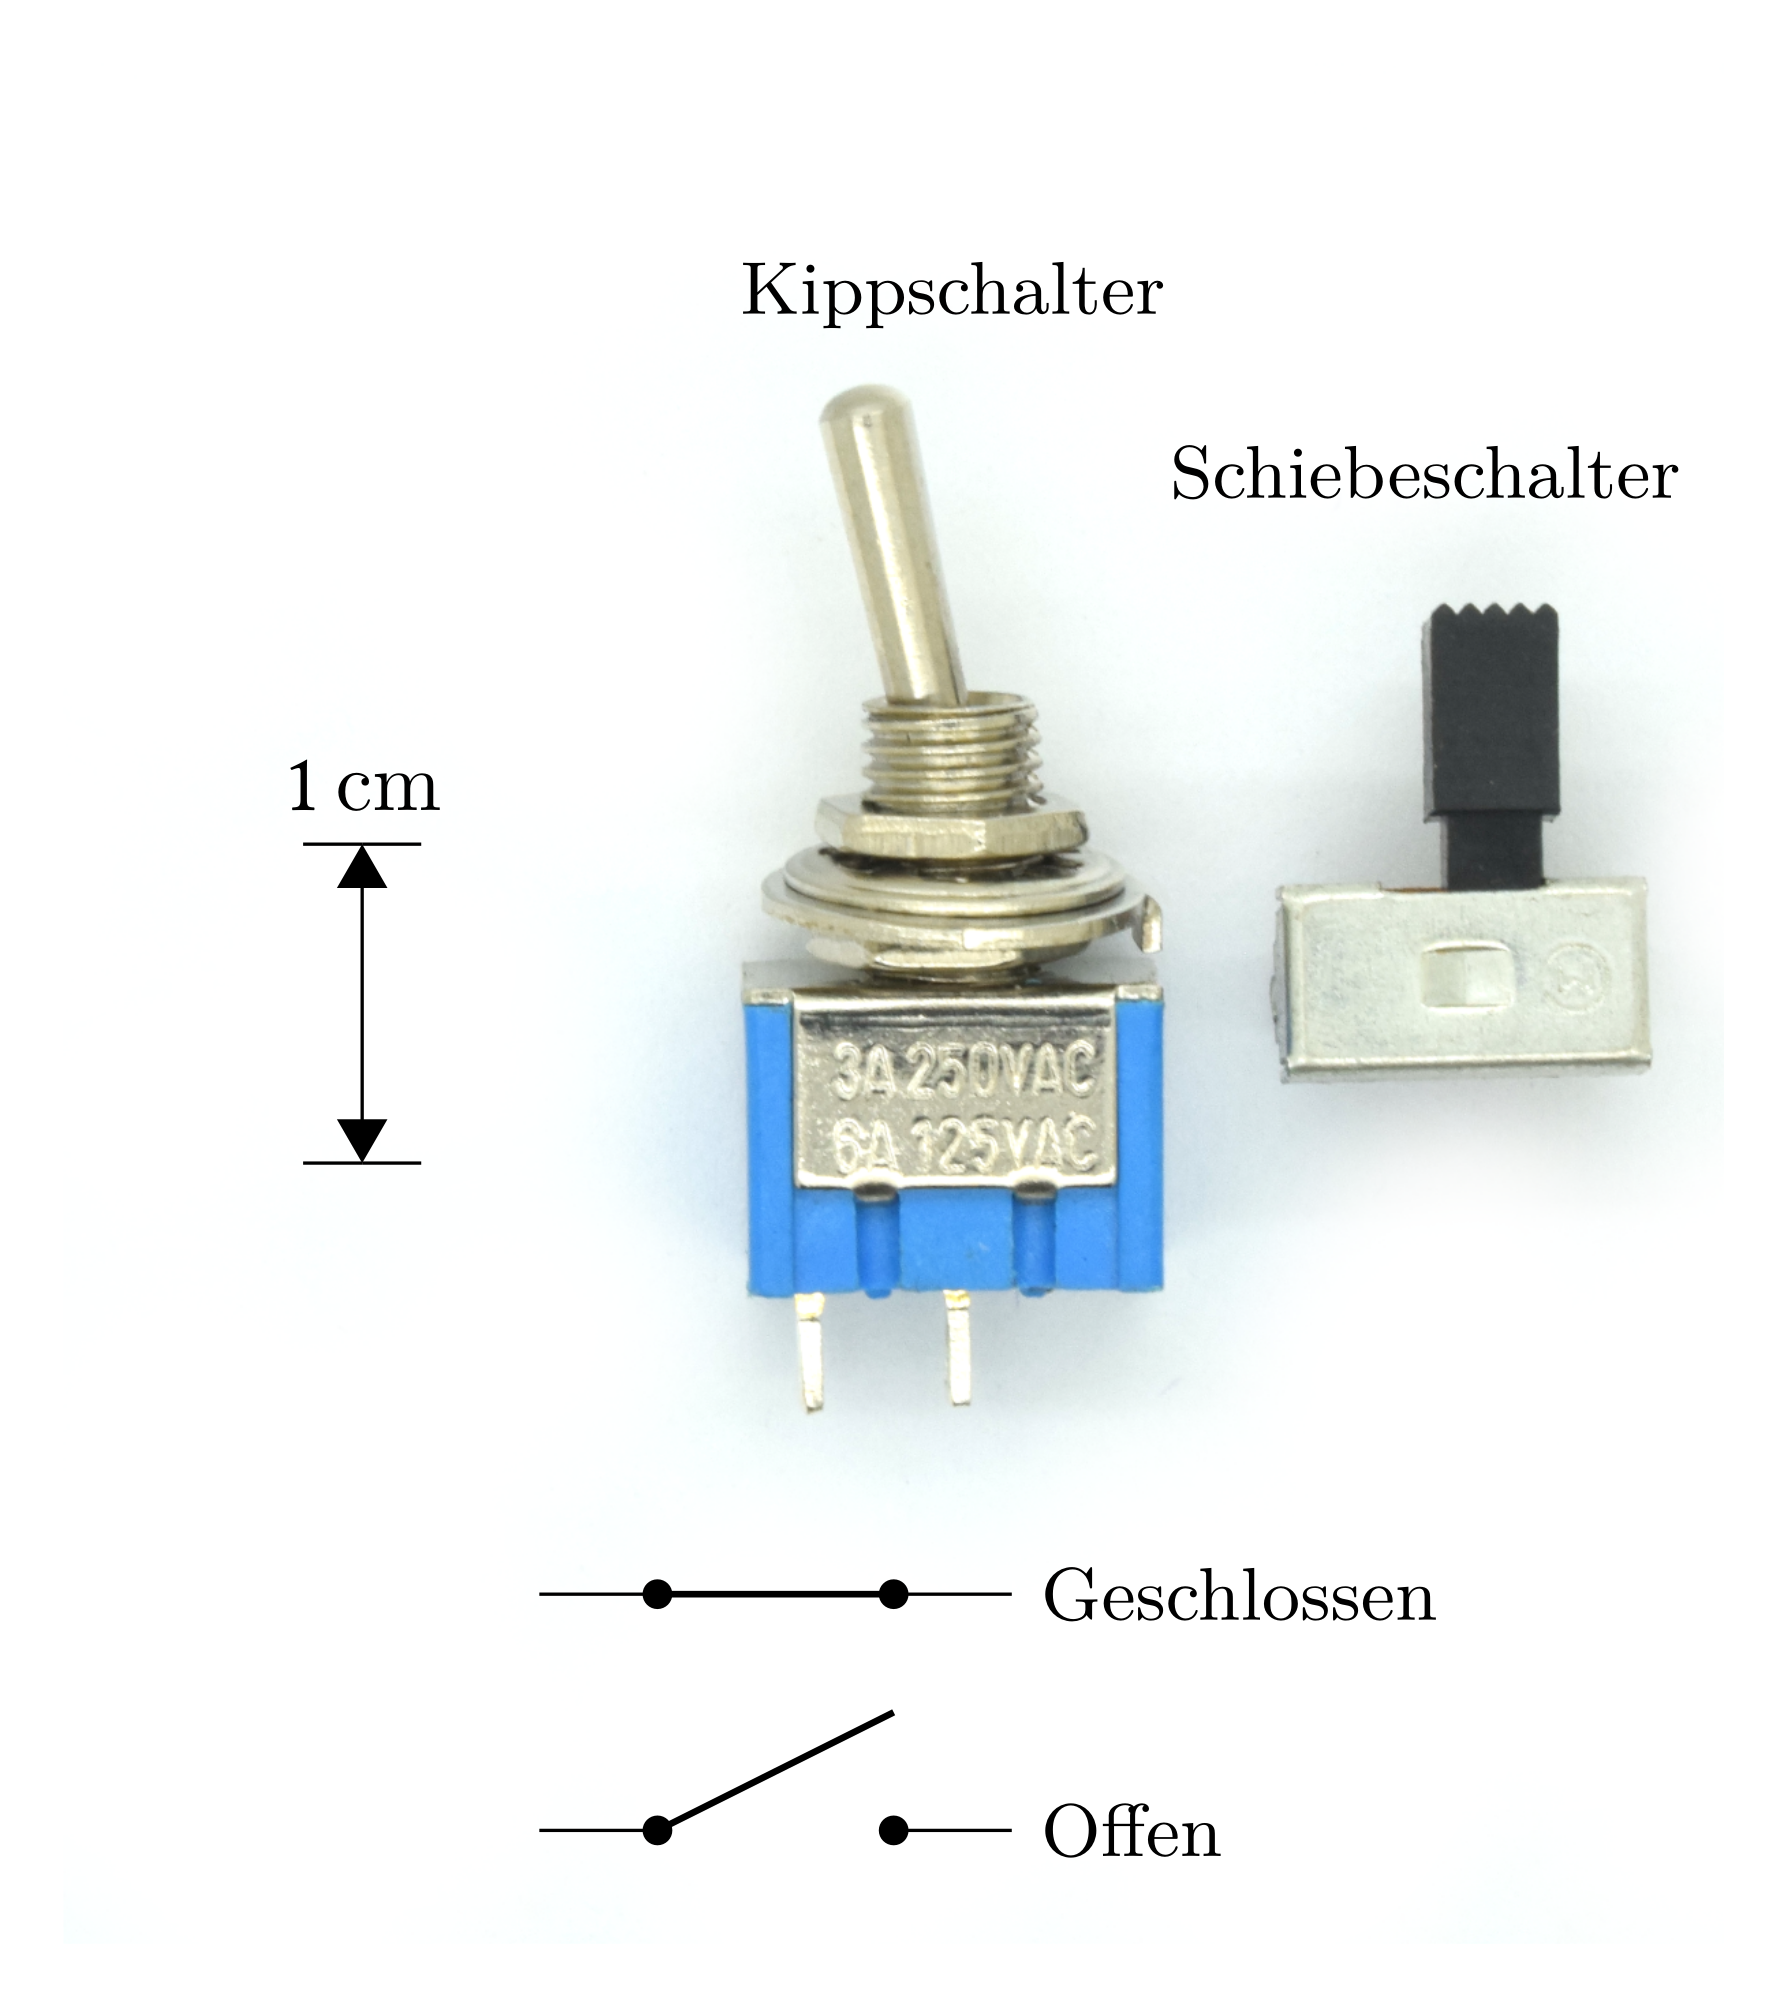
\includegraphics[width=0.85\textwidth]{foto/202}
    \caption{\scriptsize Schaltzeichen und Bauformen von Schaltern}
    \label{n_stromkreis_schalter}
\end{figure}

   \end{column}
\end{columns}

\end{frame}

\begin{frame}
\only<1>{
\begin{PQuestion}{NB701}{Welches Bauteil wird durch das Schaltzeichen symbolisiert?}{Masse}
{Schalter}
{Antenne}
{Erde}
{\DARCimage{0.5\linewidth}{546include}}\end{PQuestion}

}
\only<2>{
\begin{PQuestion}{NB701}{Welches Bauteil wird durch das Schaltzeichen symbolisiert?}{Masse}
{\textbf{\textcolor{DARCgreen}{Schalter}}}
{Antenne}
{Erde}
{\DARCimage{0.5\linewidth}{546include}}\end{PQuestion}

}
\end{frame}

\begin{frame}
\frametitle{Widerstand}
\begin{columns}
    \begin{column}{0.48\textwidth}
    \begin{itemize}
  \item Begrenzt den Stromfluss
  \item Wandelt Strom in Wärme um
  \end{itemize}

    \end{column}
   \begin{column}{0.48\textwidth}
       
\begin{figure}
    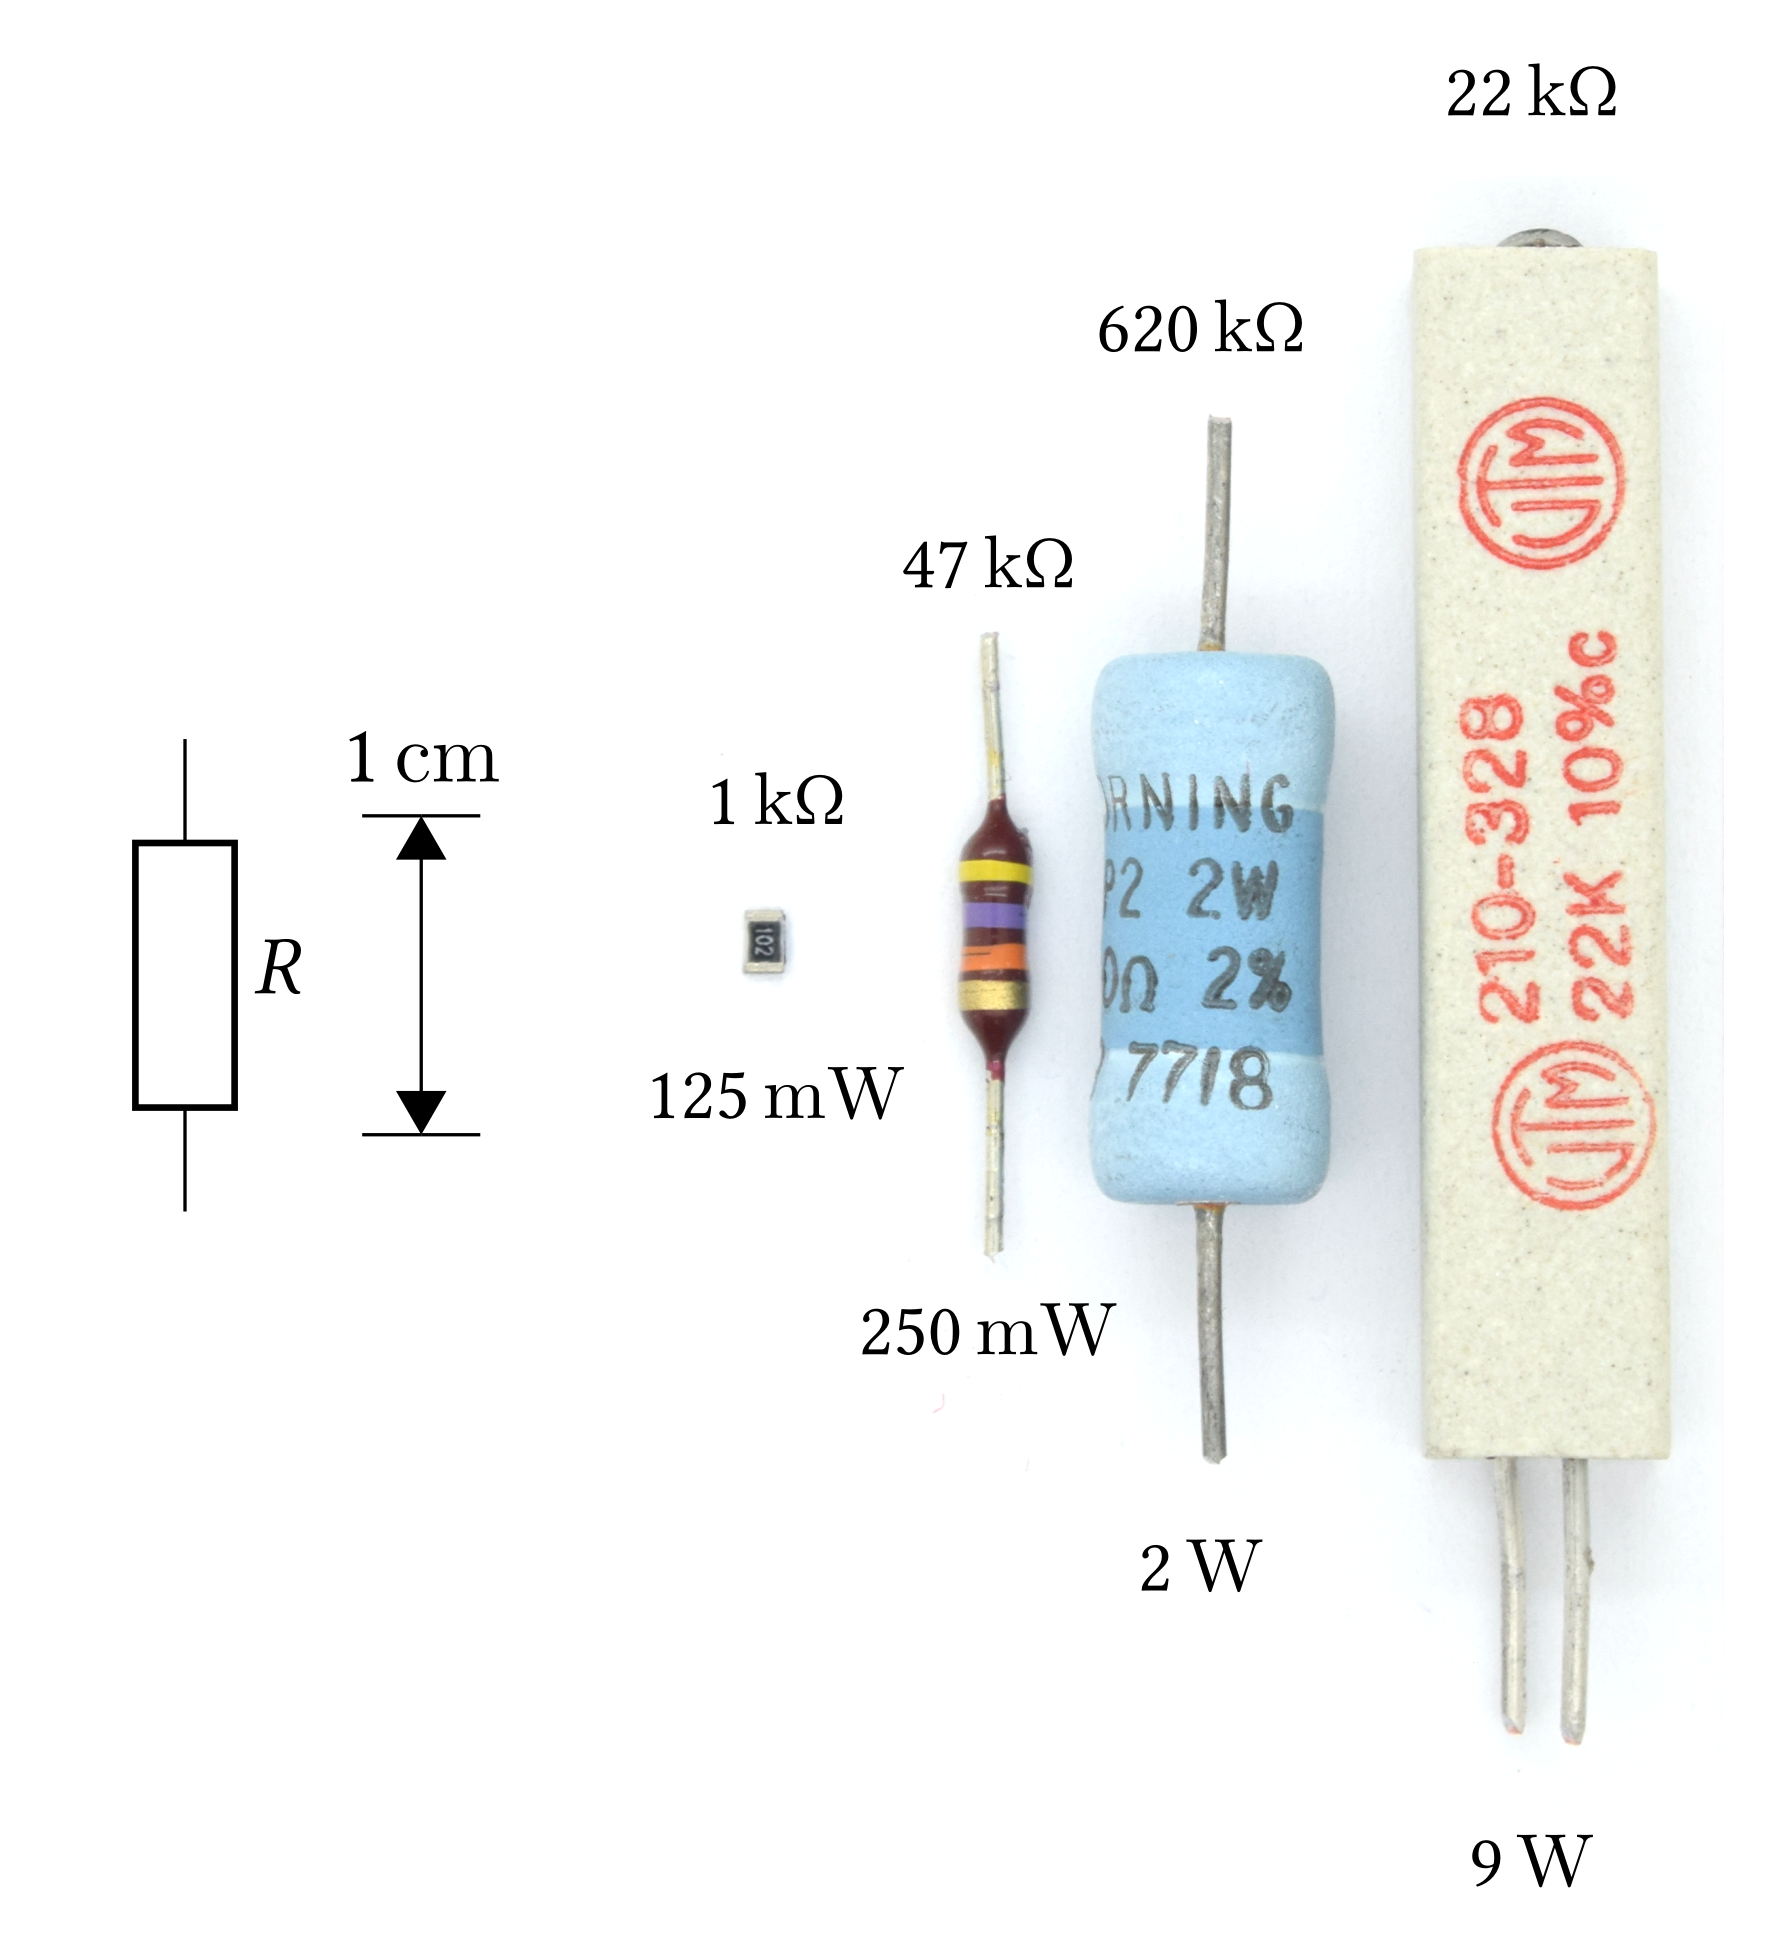
\includegraphics[width=0.85\textwidth]{foto/203}
    \caption{\scriptsize Schaltzeichen und Bauformen von Widerständen}
    \label{n_stromkreis_widerstand}
\end{figure}

   \end{column}
\end{columns}

\end{frame}

\begin{frame}
\only<1>{
\begin{PQuestion}{NC101}{Welches Bauteil wird durch das Schaltzeichen symbolisiert?}{Kondensator}
{Diode}
{Spule}
{Widerstand}
{\DARCimage{0.5\linewidth}{509include}}\end{PQuestion}

}
\only<2>{
\begin{PQuestion}{NC101}{Welches Bauteil wird durch das Schaltzeichen symbolisiert?}{Kondensator}
{Diode}
{Spule}
{\textbf{\textcolor{DARCgreen}{Widerstand}}}
{\DARCimage{0.5\linewidth}{509include}}\end{PQuestion}

}
\end{frame}

\begin{frame}
\frametitle{Stromrichtung}

\begin{figure}
    \DARCimage{0.85\linewidth}{662include}
    \caption{\scriptsize Geschlossener Stromkreis}
    \label{n_stromkreis_geschlossen}
\end{figure}

Vom Pluspol zum Minuspol: \emph{technische Stromrichtung}

\end{frame}

\begin{frame}
\only<1>{
\begin{question2x2}{NB702}{Welches Bild zeigt die technische Stromrichtung korrekt an?}{\DARCimage{1.0\linewidth}{536include}}
{\DARCimage{1.0\linewidth}{535include}}
{\DARCimage{1.0\linewidth}{537include}}
{\DARCimage{1.0\linewidth}{538include}}
\end{question2x2}

}
\only<2>{
\begin{question2x2}{NB702}{Welches Bild zeigt die technische Stromrichtung korrekt an?}{\DARCimage{1.0\linewidth}{536include}}
{\textbf{\textcolor{DARCgreen}{\DARCimage{1.0\linewidth}{535include}}}}
{\DARCimage{1.0\linewidth}{537include}}
{\DARCimage{1.0\linewidth}{538include}}
\end{question2x2}

}
\end{frame}

\begin{frame}
\only<1>{
\begin{PQuestion}{NB207}{Kann in folgender Schaltung von zwei gleichen Spannungsquellen Strom fließen? Welche Begründung ist richtig?}{Ja, weil der Pluspol mit dem Minuspol verbunden ist.}
{Nein, weil dies nur bei verschiedenen Spannungsquellen möglich ist.}
{Nein, weil kein geschlossener Stromkreis vorhanden ist.}
{Ja, weil die Spannungsquellen nie exakt identisch sind.}
{\DARCimage{1.0\linewidth}{451include}}\end{PQuestion}

}
\only<2>{
\begin{PQuestion}{NB207}{Kann in folgender Schaltung von zwei gleichen Spannungsquellen Strom fließen? Welche Begründung ist richtig?}{Ja, weil der Pluspol mit dem Minuspol verbunden ist.}
{Nein, weil dies nur bei verschiedenen Spannungsquellen möglich ist.}
{\textbf{\textcolor{DARCgreen}{Nein, weil kein geschlossener Stromkreis vorhanden ist.}}}
{Ja, weil die Spannungsquellen nie exakt identisch sind.}
{\DARCimage{1.0\linewidth}{451include}}\end{PQuestion}

}
\end{frame}%ENDCONTENT


\section{Physikalische Stromrichtung}
\label{section:physikalische_stromrichtung}
\begin{frame}%STARTCONTENT
\begin{itemize}
  \item Technische Stromrichtung vom Plus-Pol zum Minus-Pol
  \item In der Wissenschaft hat sich später erst herausgestellt, dass sich in Metallen die negativ geladenen Teilchen (Elekotronen) bewegen
  \item Elektronen werden vom Minus-Pol der Spannungsquelle abgestoßen und vom Plus-Pol angezogen
  \item Die \emph{Physikalische Stromrichtung} ist entegegen gesetzt zur technischen Stromrichtung
  \end{itemize}

\end{frame}

\begin{frame}
\only<1>{
\begin{question2x2}{AB601}{Welches Bild zeigt die physikalische Stromrichtung korrekt an?}{\DARCimage{1.0\linewidth}{646include}}
{\DARCimage{1.0\linewidth}{647include}}
{\DARCimage{1.0\linewidth}{557include}}
{\DARCimage{1.0\linewidth}{558include}}
\end{question2x2}

}
\only<2>{
\begin{question2x2}{AB601}{Welches Bild zeigt die physikalische Stromrichtung korrekt an?}{\textbf{\textcolor{DARCgreen}{\DARCimage{1.0\linewidth}{646include}}}}
{\DARCimage{1.0\linewidth}{647include}}
{\DARCimage{1.0\linewidth}{557include}}
{\DARCimage{1.0\linewidth}{558include}}
\end{question2x2}

}
\end{frame}%ENDCONTENT


\section{Spannungsmessung}
\label{section:spannungsmessung}
\begin{frame}%STARTCONTENT

\begin{columns}
    \begin{column}{0.48\textwidth}
    \begin{itemize}
  \item Spannungen lassen sich mit einem Messgerät ermitteln
  \item Schaltsymbol \enquote{V mit einem Kreis}
  \item Messgerät richtig einstellen
  \item An den richtigen Stellen messen
  \end{itemize}

    \end{column}
   \begin{column}{0.48\textwidth}
       
\begin{figure}
    \DARCimage{0.85\linewidth}{625include}
    \caption{\scriptsize Schaltsymbol Spannungsmessgerät}
    \label{n_messgeraete_symbol_spannungsmessgerät}
\end{figure}


   \end{column}
\end{columns}

\end{frame}

\begin{frame}
\frametitle{Richtig messen}
\begin{columns}
    \begin{column}{0.48\textwidth}
    \begin{itemize}
  \item Spannung wird zwischen zwei Punkten gemessen
  \item Parallel zum zu messenden Bauteil
  \end{itemize}

    \end{column}
   \begin{column}{0.48\textwidth}
       
\begin{figure}
    \DARCimage{0.85\linewidth}{620include}
    \caption{\scriptsize Spannungsmessung}
    \label{n_messgeraete_spannungsmessung}
\end{figure}


   \end{column}
\end{columns}

\end{frame}

\begin{frame}
\only<1>{
\begin{PQuestion}{NI101}{Was wird durch dieses Schaltzeichen symbolisiert?}{Stromquelle}
{Strommessgerät}
{Spannungsquelle}
{Spannungsmessgerät}
{\DARCimage{0.5\linewidth}{625include}}\end{PQuestion}

}
\only<2>{
\begin{PQuestion}{NI101}{Was wird durch dieses Schaltzeichen symbolisiert?}{Stromquelle}
{Strommessgerät}
{Spannungsquelle}
{\textbf{\textcolor{DARCgreen}{Spannungsmessgerät}}}
{\DARCimage{0.5\linewidth}{625include}}\end{PQuestion}

}
 \end{frame}

\begin{frame}
\only<1>{
\begin{question2x2}{NI103}{In welcher Schaltung ist ein Multimeter richtig eingesetzt, um die Spannung der Batterie im laufenden Betrieb zu messen?}{\DARCimage{0.75\linewidth}{623include}}
{\DARCimage{0.75\linewidth}{621include}}
{\DARCimage{0.75\linewidth}{622include}}
{\DARCimage{0.75\linewidth}{620include}}
\end{question2x2}

}
\only<2>{
\begin{question2x2}{NI103}{In welcher Schaltung ist ein Multimeter richtig eingesetzt, um die Spannung der Batterie im laufenden Betrieb zu messen?}{\DARCimage{0.75\linewidth}{623include}}
{\DARCimage{0.75\linewidth}{621include}}
{\DARCimage{0.75\linewidth}{622include}}
{\textbf{\textcolor{DARCgreen}{\DARCimage{0.75\linewidth}{620include}}}}
\end{question2x2}

}
\end{frame}

\begin{frame}
\only<1>{
\begin{PQuestion}{NB205}{Welchen Betrag zeigt das Spannungsmessgerät in folgender Schaltung? }{\qty{0}{\V}}
{\qty{3}{\V}}
{\qty{2,25}{\V}}
{\qty{1,5}{\V}}
{\DARCimage{1.0\linewidth}{626include}}\end{PQuestion}

}
\only<2>{
\begin{PQuestion}{NB205}{Welchen Betrag zeigt das Spannungsmessgerät in folgender Schaltung? }{\qty{0}{\V}}
{\textbf{\textcolor{DARCgreen}{\qty{3}{\V}}}}
{\qty{2,25}{\V}}
{\qty{1,5}{\V}}
{\DARCimage{1.0\linewidth}{626include}}\end{PQuestion}

}

\end{frame}

\begin{frame}
\only<1>{
\begin{PQuestion}{NB206}{Welche Spannung zeigt das Spannungsmessgerät in folgender Schaltung? }{\qty{1,5}{\V}}
{\qty{3}{\V}}
{\qty{-3}{\V}}
{\qty{0}{\V}}
{\DARCimage{1.0\linewidth}{452include}}\end{PQuestion}

}
\only<2>{
\begin{PQuestion}{NB206}{Welche Spannung zeigt das Spannungsmessgerät in folgender Schaltung? }{\qty{1,5}{\V}}
{\qty{3}{\V}}
{\qty{-3}{\V}}
{\textbf{\textcolor{DARCgreen}{\qty{0}{\V}}}}
{\DARCimage{1.0\linewidth}{452include}}\end{PQuestion}

}

\end{frame}%ENDCONTENT


\section{Strom messen}
\label{section:strommessung}
\begin{frame}%STARTCONTENT

\begin{columns}
    \begin{column}{0.48\textwidth}
    \begin{itemize}
  \item Strommessgeräte messen den elektischen Strom
  \item Schaltsymbol \enquote{A in einem Kreis} 
  \end{itemize}

    \end{column}
   \begin{column}{0.48\textwidth}
       
\begin{figure}
    \DARCimage{0.85\linewidth}{624include}
    \caption{\scriptsize Schaltsymbol Strommessgerät}
    \label{n_messgeraete_symbol_strommessgerät}
\end{figure}


   \end{column}
\end{columns}

\end{frame}

\begin{frame}
\frametitle{Richtig messen}
\begin{columns}
    \begin{column}{0.48\textwidth}
    \begin{itemize}
  \item Strom wird in Serie mit den Bauteilen gemessen
  \item Dadurch wird die Stromstärke durch das Bauteil ermittelt
  \end{itemize}

    \end{column}
   \begin{column}{0.48\textwidth}
       
\begin{figure}
    \DARCimage{0.85\linewidth}{616include}
    \caption{\scriptsize Strommessung}
    \label{n_messgeraete_strommessung}
\end{figure}


   \end{column}
\end{columns}

\end{frame}

\begin{frame}
\only<1>{
\begin{PQuestion}{NI102}{Was wird durch dieses Schaltzeichen symbolisiert?}{Spannungsquelle}
{Stromquelle}
{Spannungsmessgerät}
{Strommessgerät}
{\DARCimage{0.5\linewidth}{624include}}\end{PQuestion}

}
\only<2>{
\begin{PQuestion}{NI102}{Was wird durch dieses Schaltzeichen symbolisiert?}{Spannungsquelle}
{Stromquelle}
{Spannungsmessgerät}
{\textbf{\textcolor{DARCgreen}{Strommessgerät}}}
{\DARCimage{0.5\linewidth}{624include}}\end{PQuestion}

}
\end{frame}

\begin{frame}
\only<1>{
\begin{question2x2}{NI104}{In welcher Schaltung ist ein Multimeter richtig eingesetzt, um den Strom durch den Widerstand und die LED zu messen? }{\DARCimage{0.75\linewidth}{618include}}
{\DARCimage{0.75\linewidth}{617include}}
{\DARCimage{0.75\linewidth}{616include}}
{\DARCimage{0.75\linewidth}{619include}}
\end{question2x2}

}
\only<2>{
\begin{question2x2}{NI104}{In welcher Schaltung ist ein Multimeter richtig eingesetzt, um den Strom durch den Widerstand und die LED zu messen? }{\DARCimage{0.75\linewidth}{618include}}
{\DARCimage{0.75\linewidth}{617include}}
{\textbf{\textcolor{DARCgreen}{\DARCimage{0.75\linewidth}{616include}}}}
{\DARCimage{0.75\linewidth}{619include}}
\end{question2x2}

}
\end{frame}%ENDCONTENT


\section{Strom- und Spannungsmessung II}
\label{section:strom_spannung_messung_2}
\begin{frame}%STARTCONTENT

\begin{columns}
    \begin{column}{0.48\textwidth}
    \begin{itemize}
  \item Der Strom wird im Stromkreis eingeschleift gemessen
  \item Die Spannung wird über den Widerstand gemessen
  \item Der Widerstand im Voltmeter soll hochohmig sein $\rightarrow$ Strom nimmt den Weg des geringsten Widerstandes
  \end{itemize}

    \end{column}
   \begin{column}{0.48\textwidth}
       
\begin{figure}
    \DARCimage{0.85\linewidth}{238include}
    \caption{\scriptsize Korrekte Anordnung zur Messung von Strom und Spannung an einem Widerstand}
    \label{e_strom_und_spannungsmessung}
\end{figure}


   \end{column}
\end{columns}

\end{frame}

\begin{frame}
\only<1>{
\begin{QQuestion}{EI101}{Wie werden elektrische Spannungsmessgeräte an Messobjekte angeschlossen und welche Anforderungen muss das Messgerät erfüllen, damit der Messfehler möglichst gering bleibt? Das Spannungsmessgerät ist~...}{in den Stromkreis einzuschleifen und sollte niederohmig sein.}
{parallel zum Messobjekt anzuschließen und sollte hochohmig sein.}
{parallel zum Messobjekt anzuschließen und sollte niederohmig sein.}
{in den Stromkreis einzuschleifen und sollte hochohmig sein.}
\end{QQuestion}

}
\only<2>{
\begin{QQuestion}{EI101}{Wie werden elektrische Spannungsmessgeräte an Messobjekte angeschlossen und welche Anforderungen muss das Messgerät erfüllen, damit der Messfehler möglichst gering bleibt? Das Spannungsmessgerät ist~...}{in den Stromkreis einzuschleifen und sollte niederohmig sein.}
{\textbf{\textcolor{DARCgreen}{parallel zum Messobjekt anzuschließen und sollte hochohmig sein.}}}
{parallel zum Messobjekt anzuschließen und sollte niederohmig sein.}
{in den Stromkreis einzuschleifen und sollte hochohmig sein.}
\end{QQuestion}

}
\end{frame}

\begin{frame}
\only<1>{
\begin{question2x2}{EI102}{Welche Schaltung mit idealen Messgeräten könnte dazu verwendet werden, den Wert eines Widerstandes anhand des ohmschen Gesetzes zu ermitteln?}{\DARCimage{0.75\linewidth}{240include}}
{\DARCimage{0.75\linewidth}{239include}}
{\DARCimage{0.75\linewidth}{241include}}
{\DARCimage{0.75\linewidth}{238include}}
\end{question2x2}

}
\only<2>{
\begin{question2x2}{EI102}{Welche Schaltung mit idealen Messgeräten könnte dazu verwendet werden, den Wert eines Widerstandes anhand des ohmschen Gesetzes zu ermitteln?}{\DARCimage{0.75\linewidth}{240include}}
{\DARCimage{0.75\linewidth}{239include}}
{\DARCimage{0.75\linewidth}{241include}}
{\textbf{\textcolor{DARCgreen}{\DARCimage{0.75\linewidth}{238include}}}}
\end{question2x2}

}
\end{frame}%ENDCONTENT


\section{Strom- und Spannungsmessung III}
\label{section:strom_spannung_messung_3}
\begin{frame}%STARTCONTENT

\frametitle{Foliensatz in Arbeit}
2024-04-28: Die Inhalte werden noch aufbereitet.

Derzeit sind in diesem Abschnitt nur die Fragen sortiert enthalten.

Für das Selbststudium verweisen wir aktuell auf den Abschnitt Messtechnik im DARC Online Lehrgang (\textcolor{DARCblue}{\faLink~\href{https://www.darc.de/der-club/referate/ajw/lehrgang-ta/a16/}{www.darc.de/der-club/referate/ajw/lehrgang-ta/a16/}}) für die Prüfung bis Juni 2024. Bis auf die Fragen hat sich an der Thematik nichts geändert.

\end{frame}

\begin{frame}
\frametitle{Strom- und Spannungsmessung}
\end{frame}

\begin{frame}
\only<1>{
\begin{PQuestion}{AI101}{Wie sollten Strom- und Spannungsmessgeräte zur Feststellung der Gleichstrom-Eingangsleistung des dargestellten Endverstärkers (PA) angeordnet werden?}{Spannungsmessgerät bei 3, Strommessgerät bei 1.}
{Spannungsmessgerät bei 1, Strommessgerät bei 2.}
{Spannungsmessgerät bei 1, Strommessgerät bei 3.}
{Spannungsmessgerät bei 3, Strommessgerät bei 4.}
{\DARCimage{1.0\linewidth}{443include}}\end{PQuestion}

}
\only<2>{
\begin{PQuestion}{AI101}{Wie sollten Strom- und Spannungsmessgeräte zur Feststellung der Gleichstrom-Eingangsleistung des dargestellten Endverstärkers (PA) angeordnet werden?}{Spannungsmessgerät bei 3, Strommessgerät bei 1.}
{Spannungsmessgerät bei 1, Strommessgerät bei 2.}
{\textbf{\textcolor{DARCgreen}{Spannungsmessgerät bei 1, Strommessgerät bei 3.}}}
{Spannungsmessgerät bei 3, Strommessgerät bei 4.}
{\DARCimage{1.0\linewidth}{443include}}\end{PQuestion}

}
\end{frame}

\begin{frame}
\only<1>{
\begin{PQuestion}{AI102}{Für die Messung der Gleichstrom-Eingangsleistung werden verschiedene Messgeräte verwendet. Bei welchen der Instrumente in der Abbildung handelt es sich um Strommessgeräte?}{2, 3 und 4}
{1, 2 und 3}
{2, 4 und 1}
{1, 3 und 4}
{\DARCimage{1.0\linewidth}{443include}}\end{PQuestion}

}
\only<2>{
\begin{PQuestion}{AI102}{Für die Messung der Gleichstrom-Eingangsleistung werden verschiedene Messgeräte verwendet. Bei welchen der Instrumente in der Abbildung handelt es sich um Strommessgeräte?}{\textbf{\textcolor{DARCgreen}{2, 3 und 4}}}
{1, 2 und 3}
{2, 4 und 1}
{1, 3 und 4}
{\DARCimage{1.0\linewidth}{443include}}\end{PQuestion}

}
\end{frame}

\begin{frame}
\frametitle{Messgenauigkeit}
\end{frame}

\begin{frame}
\only<1>{
\begin{QQuestion}{AI103}{Ein Spannungs- und ein Strommessgerät werden für die Ermittlung der Gleichstromeingangsleistung einer Schaltung verwendet. Das Spannungsmessgerät zeigt \qty{10}{\V}, das Strommessgerät \qty{10}{\A} an. Falls beide dabei im Rahmen ihrer Messgenauigkeit jeweils einen um \qty{5}{\percent} zu geringen Wert anzeigen würden, würde man die elektrische Leistung um~...}{\qty{5}{\percent} zu hoch bestimmen.}
{\qty{5}{\percent} zu niedrig bestimmen.}
{\qty{10,25}{\percent} zu hoch bestimmen.}
{\qty{9,75}{\percent} zu niedrig bestimmen.}
\end{QQuestion}

}
\only<2>{
\begin{QQuestion}{AI103}{Ein Spannungs- und ein Strommessgerät werden für die Ermittlung der Gleichstromeingangsleistung einer Schaltung verwendet. Das Spannungsmessgerät zeigt \qty{10}{\V}, das Strommessgerät \qty{10}{\A} an. Falls beide dabei im Rahmen ihrer Messgenauigkeit jeweils einen um \qty{5}{\percent} zu geringen Wert anzeigen würden, würde man die elektrische Leistung um~...}{\qty{5}{\percent} zu hoch bestimmen.}
{\qty{5}{\percent} zu niedrig bestimmen.}
{\qty{10,25}{\percent} zu hoch bestimmen.}
{\textbf{\textcolor{DARCgreen}{\qty{9,75}{\percent} zu niedrig bestimmen.}}}
\end{QQuestion}

}
\end{frame}

\begin{frame}
\frametitle{Lösungsweg}
\begin{itemize}
  \item Prozentrechnung – die absoluten Werte sind nicht relevant
  \item gegeben: $U_{\textrm{Abw}}$ mit \qty{95}{\percent} vom Realwert
  \item gegeben: $I_{\textrm{Abw}}$ mit \qty{95}{\percent} vom Realwert
  \item gesucht: Abweichung der Leistung $P = U \cdot I$
  \end{itemize}
    \pause
    \begin{equation}\begin{split} \nonumber P_{\textrm{Abw}} &= 100\% -- (U_{\textrm{Abw}} \cdot I_{\textrm{Abw}})\\ &= 100\% -- (95\% \cdot 95\%)\\ &= 100\% -- 90,25\%\\ &= 9,75\% \end{split}\end{equation}



\end{frame}

\begin{frame}
\frametitle{Strom durch Multimeter}
\end{frame}

\begin{frame}
\only<1>{
\begin{QQuestion}{AI104}{Für ein digitales Multimeter ist folgende Angabe im Datenblatt zu finden: Kleinste Auflösung \qty{100}{\micro\V}, Innenwiderstand \qty{10}{\Mohm} in allen Messbereichen. Sie messen eine Spannung von \qty{0,5}{\V}. Welcher Strom fließt dabei durch das Multimeter?}{50~nA}
{10~nA}
{500~nA}
{200~nA}
\end{QQuestion}

}
\only<2>{
\begin{QQuestion}{AI104}{Für ein digitales Multimeter ist folgende Angabe im Datenblatt zu finden: Kleinste Auflösung \qty{100}{\micro\V}, Innenwiderstand \qty{10}{\Mohm} in allen Messbereichen. Sie messen eine Spannung von \qty{0,5}{\V}. Welcher Strom fließt dabei durch das Multimeter?}{\textbf{\textcolor{DARCgreen}{50~nA}}}
{10~nA}
{500~nA}
{200~nA}
\end{QQuestion}

}
\end{frame}

\begin{frame}
\frametitle{Lösungsweg}
\begin{itemize}
  \item gegeben: $U = 0,5V$
  \item gegeben: $R = 10M\Omega$
  \item gesucht: $I$
  \end{itemize}
    \pause
    \begin{equation} \nonumber I = \frac{U}{R} = \frac{0,5V}{10M\Omega} = 50nA \end{equation}



\end{frame}

\begin{frame}
\frametitle{Thermoumformer}
\begin{itemize}
  \item Messgerät, bei dem die abgestrahlte Wärme an einem Widerstand gemessen wird
  \item Aus der abgestrahlten Wärme wird mit einem Thermoelement eine Gleichspannung erzeugt, die gemessen werden kann
  \item Wird dann eingesetzt, wenn eine elektrische Messung nicht möglich ist, z.B. bei nicht-periodischen Signalen
  \end{itemize}
\end{frame}

\begin{frame}
\only<1>{
\begin{QQuestion}{AI105}{Zur genauen Messung der effektiven Leistung eines modulierten Signals bis in den oberen GHz-Bereich eignet sich~...}{ein Digitalmultimeter.}
{ein Oszillograf.}
{ein Messgerät mit Diodentastkopf.}
{ein Messgerät mit Thermoumformer.}
\end{QQuestion}

}
\only<2>{
\begin{QQuestion}{AI105}{Zur genauen Messung der effektiven Leistung eines modulierten Signals bis in den oberen GHz-Bereich eignet sich~...}{ein Digitalmultimeter.}
{ein Oszillograf.}
{ein Messgerät mit Diodentastkopf.}
{\textbf{\textcolor{DARCgreen}{ein Messgerät mit Thermoumformer.}}}
\end{QQuestion}

}
\end{frame}%ENDCONTENT


\section{Zeigerinstrumente ablesen}
\label{section:zeigerinstrumente_ablesen}
\begin{frame}%STARTCONTENT

\begin{columns}
    \begin{column}{0.48\textwidth}
    \begin{itemize}
  \item Richtige Auswahl der zu messenden Größe mit dem Schalter wählen
  \item Richtige Skala anhand des Messbereichs wählen
  \item Ggf. muss um einen Faktor 10 oder 100 multipliziert oder dividiert werden
  \item Vorteil: Man sieht kontinuierliche Änderungen
  \end{itemize}

    \end{column}
   \begin{column}{0.48\textwidth}
       
\begin{figure}
    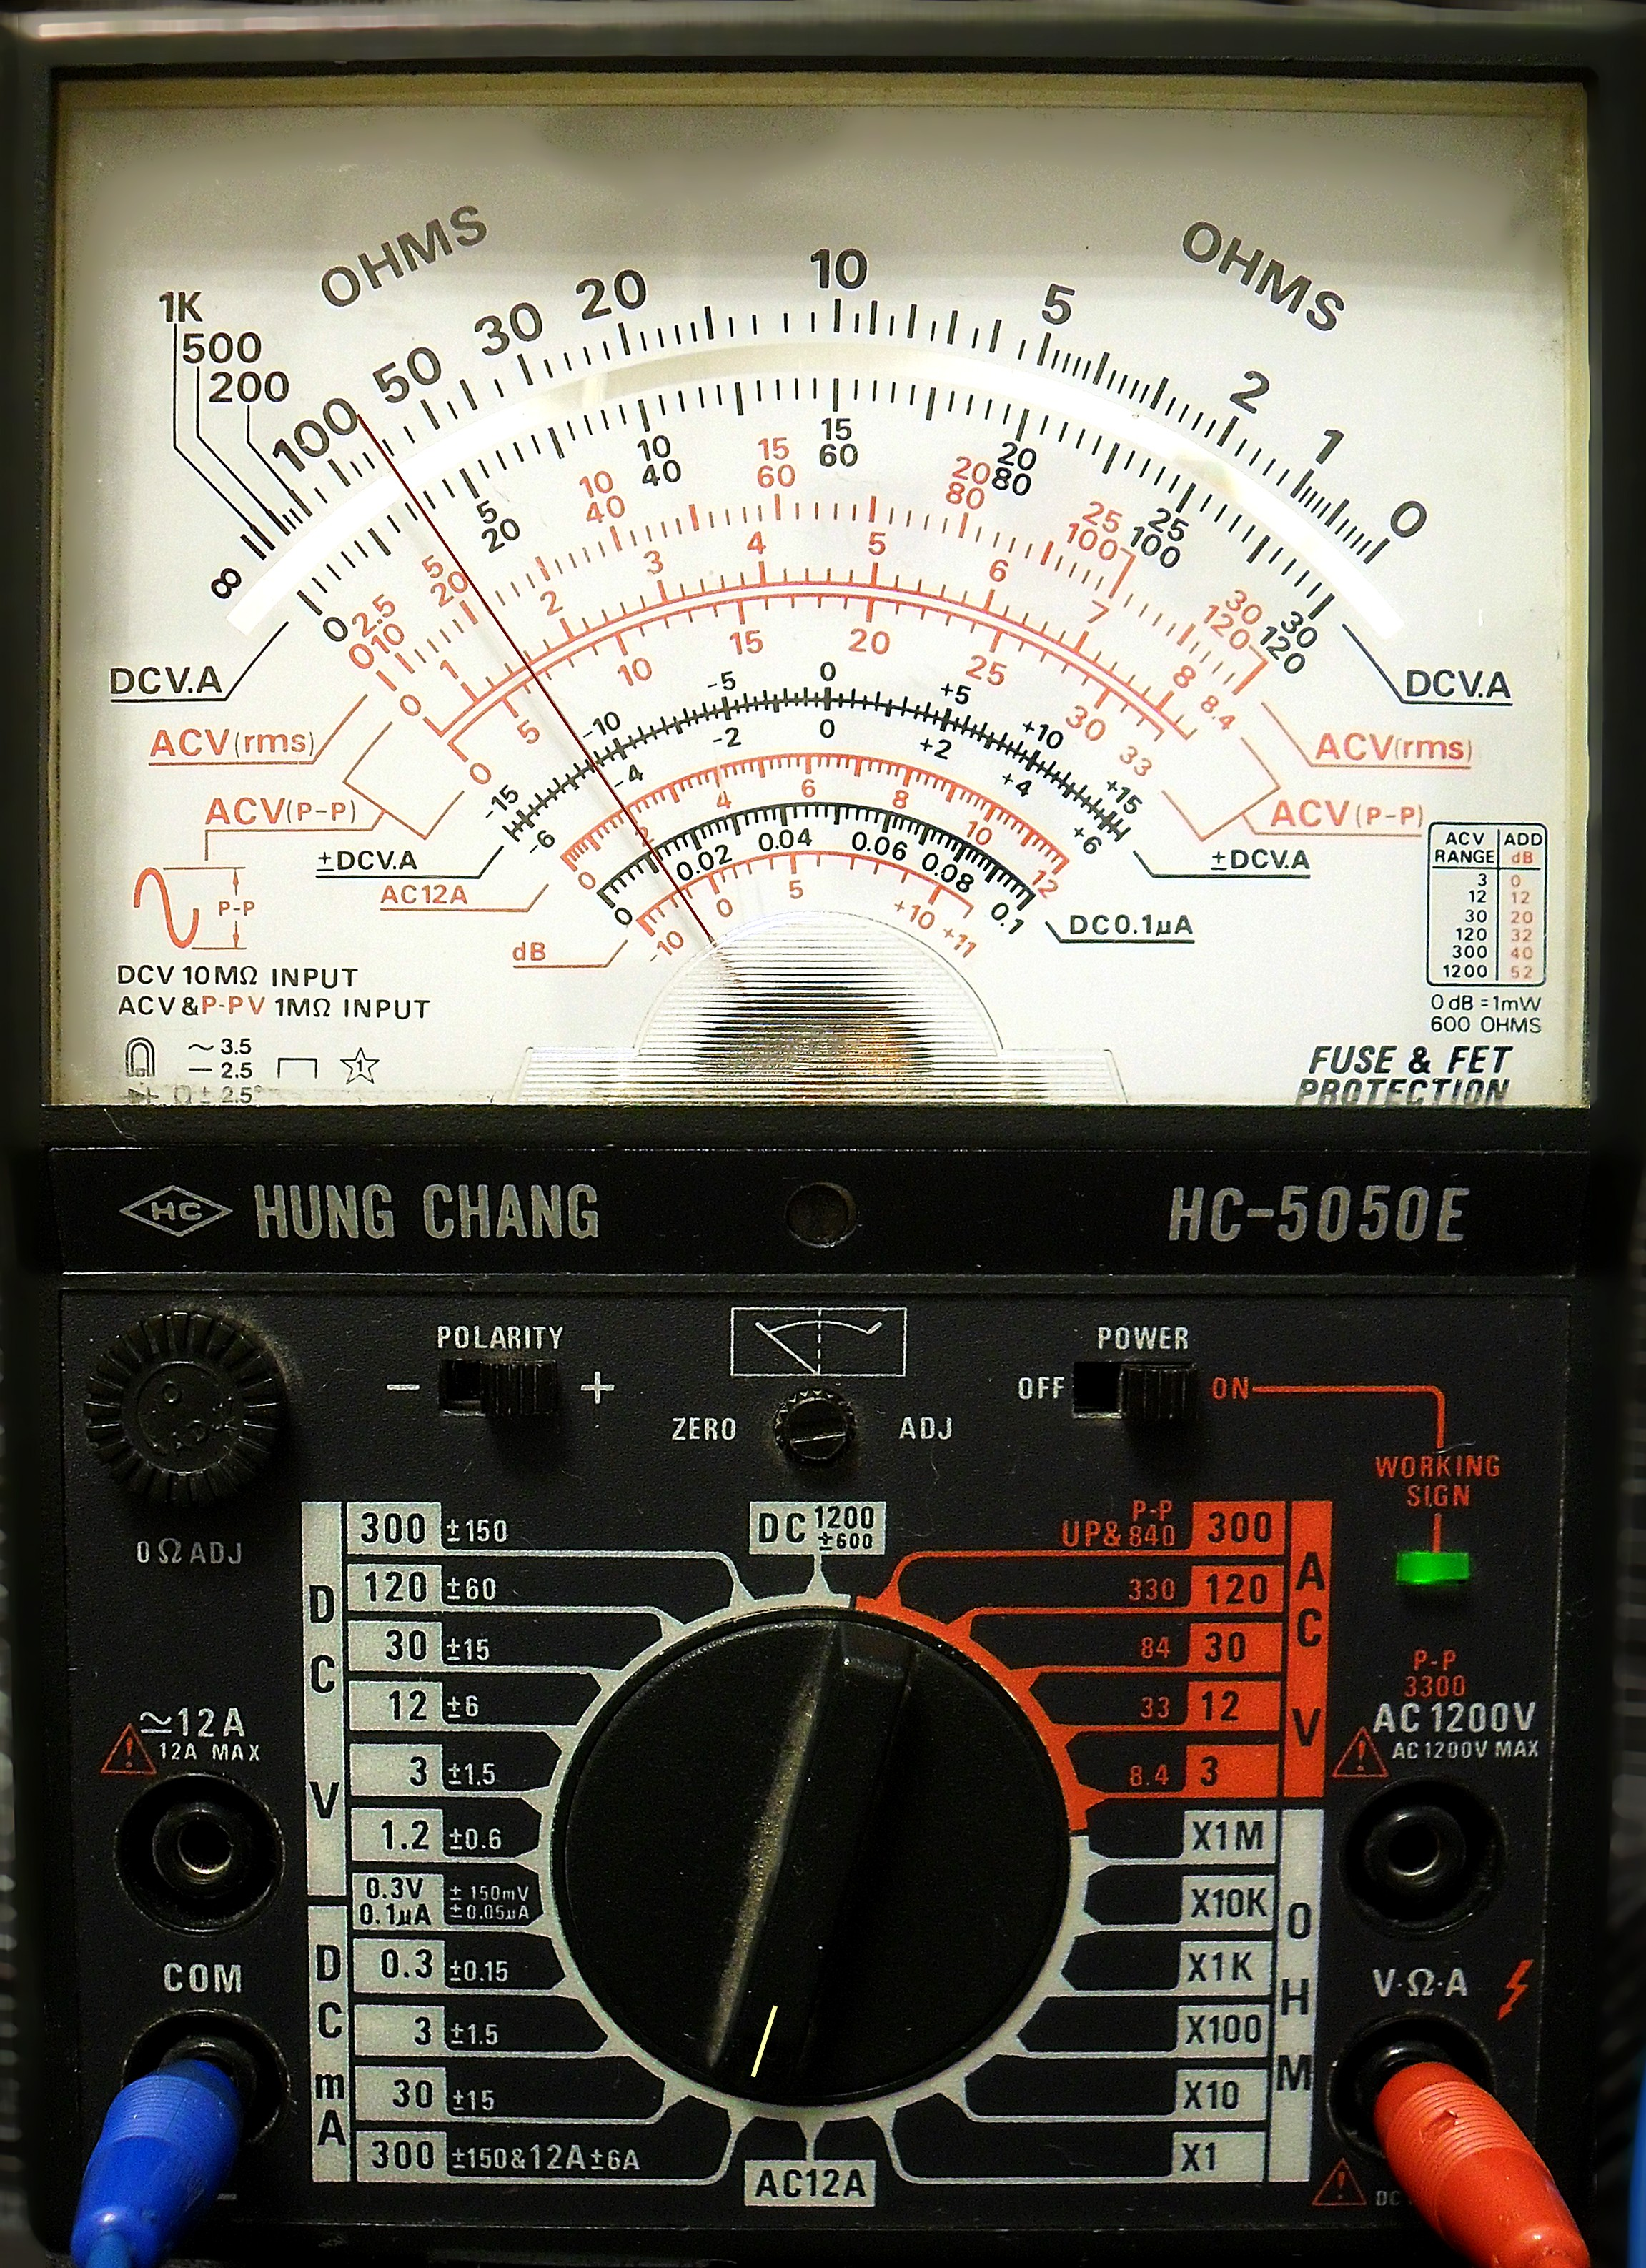
\includegraphics[width=0.85\textwidth]{foto/197}
    \caption{\scriptsize Zeigerinstrument mit mehreren Skalen}
    \label{e_zeigerinstrument}
\end{figure}

   \end{column}
\end{columns}

\end{frame}

\begin{frame}
\frametitle{Parallaxenfehler}
\begin{columns}
    \begin{column}{0.48\textwidth}
    \begin{itemize}
  \item Parallaxenfehler vermeiden, indem gerade drauf geschaut wird
  \item Viele Zeigerinstrumente haben einen Spiegel hinter dem Zeiger
  \item Wenn der Zeiger sich im Spiegelbild überdeckt, wird gerade drauf geschaut
  \end{itemize}

    \end{column}
   \begin{column}{0.48\textwidth}
       
\begin{figure}
    \includegraphics[width=0.85\textwidth]{foto/196}
    \caption{\scriptsize Zeigerinstrument mit Spiegel und Parallaxenfehler beim Ablesen}
    \label{e_parallaxenfehler}
\end{figure}

   \end{column}
\end{columns}

\end{frame}

\begin{frame}
\only<1>{
\begin{PQuestion}{EI103}{Welche Spannung wird bei dem folgenden Messinstrument angezeigt, wenn dessen Messbereich auf \qty{10}{\V} eingestellt ist? }{\qty{8,8}{\V}}
{\qty{29}{\V}}
{\qty{2,9}{\V}}
{\qty{88}{\V}}
{\DARCimage{1.0\linewidth}{41include}}\end{PQuestion}

}
\only<2>{
\begin{PQuestion}{EI103}{Welche Spannung wird bei dem folgenden Messinstrument angezeigt, wenn dessen Messbereich auf \qty{10}{\V} eingestellt ist? }{\qty{8,8}{\V}}
{\qty{29}{\V}}
{\textbf{\textcolor{DARCgreen}{\qty{2,9}{\V}}}}
{\qty{88}{\V}}
{\DARCimage{1.0\linewidth}{41include}}\end{PQuestion}

}
\end{frame}

\begin{frame}
\only<1>{
\begin{PQuestion}{EI104}{Welche Spannung wird bei dem folgenden Messinstrument angezeigt, wenn dessen Messbereich auf \qty{300}{\V} eingestellt ist?}{\qty{290}{\V}}
{\qty{29}{\V}}
{\qty{8,8}{\V}}
{\qty{88}{\V}}
{\DARCimage{1.0\linewidth}{41include}}\end{PQuestion}

}
\only<2>{
\begin{PQuestion}{EI104}{Welche Spannung wird bei dem folgenden Messinstrument angezeigt, wenn dessen Messbereich auf \qty{300}{\V} eingestellt ist?}{\qty{290}{\V}}
{\qty{29}{\V}}
{\qty{8,8}{\V}}
{\textbf{\textcolor{DARCgreen}{\qty{88}{\V}}}}
{\DARCimage{1.0\linewidth}{41include}}\end{PQuestion}

}
\end{frame}%ENDCONTENT


\section{Spitzen- und Effektivwert}
\label{section:spitze_effektiv_wert}
\begin{frame}%STARTCONTENT

\frametitle{Spitzenwert}
\begin{columns}
    \begin{column}{0.48\textwidth}
    \begin{itemize}
  \item Der Spitzenwert einer Sinusschwingung entspricht der Amplitude
  \item Von Nulllinie bis höchstem Wert
  \item Spitzen-Spitzen-Wert von niedrigstem bis höchstem Wert
  \end{itemize}

    \end{column}
   \begin{column}{0.48\textwidth}
       
\begin{figure}
    \DARCimage{0.85\linewidth}{834include}
    \caption{\scriptsize Peridoendauer, Spitzenspannung, Effektivspannung und Spitzen-Spitzen-Spannung}
    \label{e_spitze_effektiv_wert_bezeichnungen_sinus}
\end{figure}


   \end{column}
\end{columns}

\end{frame}

\begin{frame}Spitzen-Spitzen-Wert bei sinusförmigen Spannungen

$U_{SS} = 2\cdot \^{U}$

\end{frame}

\begin{frame}
\only<1>{
\begin{PQuestion}{EB407}{Wie groß ist der Spitzen-Spitzen-Wert ($U_{\symup{ss}}$) der in der Abbildung dargestellten Spannung?}{\qty{10}{\V}}
{\qty{20}{\V}}
{\qty{40}{\V}}
{\qty{4}{\V}}
{\DARCimage{1.0\linewidth}{52include}}\end{PQuestion}

}
\only<2>{
\begin{PQuestion}{EB407}{Wie groß ist der Spitzen-Spitzen-Wert ($U_{\symup{ss}}$) der in der Abbildung dargestellten Spannung?}{\qty{10}{\V}}
{\qty{20}{\V}}
{\textbf{\textcolor{DARCgreen}{\qty{40}{\V}}}}
{\qty{4}{\V}}
{\DARCimage{1.0\linewidth}{52include}}\end{PQuestion}

}
\end{frame}

\begin{frame}
\only<1>{
\begin{PQuestion}{EB406}{Wie groß ist der Spitzen-Spitzen-Wert der in diesem Schirmbild dargestellten Spannung?}{\qty{12}{\V}}
{\qty{6}{\V}}
{\qty{8,5}{\V}}
{\qty{2}{\V}}
{\DARCimage{1.0\linewidth}{53include}}\end{PQuestion}

}
\only<2>{
\begin{PQuestion}{EB406}{Wie groß ist der Spitzen-Spitzen-Wert der in diesem Schirmbild dargestellten Spannung?}{\textbf{\textcolor{DARCgreen}{\qty{12}{\V}}}}
{\qty{6}{\V}}
{\qty{8,5}{\V}}
{\qty{2}{\V}}
{\DARCimage{1.0\linewidth}{53include}}\end{PQuestion}

}
\end{frame}

\begin{frame}
\frametitle{Effektivwert}
Bei einer Wechselspannung der Wert, der in einem Widerstand zu einer vergleichsweisen Gleichspannung in Leistung umgesetzt wird


\begin{figure}
    \DARCimage{0.85\linewidth}{725include}
    \caption{\scriptsize Effektivwert und Spitzenwert der Spannung im Haushalt}
    \label{e_effektivwert_230v}
\end{figure}

\end{frame}

\begin{frame}Bei Spannungen (ohne Herleitung)

$\^{U} = U_{eff}\cdot \sqrt{2}$

\end{frame}

\begin{frame}
\only<1>{
\begin{PQuestion}{EB405}{Welche der im folgenden Diagramm eingezeichneten Gleichspannungen setzen an einem Wirkwiderstand etwa die gleiche Leistung um wie die dargestellte sinusförmige Wechselspannung?}{\qty{0}{\V}}
{\qty{1}{\V} und \qty{-1}{\V}}
{\qty{0,5}{\V} und \qty{-0,5}{\V}}
{\qty{0,7}{\V} und \qty{-0,7}{\V}}
{\DARCimage{1.0\linewidth}{206include}}\end{PQuestion}

}
\only<2>{
\begin{PQuestion}{EB405}{Welche der im folgenden Diagramm eingezeichneten Gleichspannungen setzen an einem Wirkwiderstand etwa die gleiche Leistung um wie die dargestellte sinusförmige Wechselspannung?}{\qty{0}{\V}}
{\qty{1}{\V} und \qty{-1}{\V}}
{\qty{0,5}{\V} und \qty{-0,5}{\V}}
{\textbf{\textcolor{DARCgreen}{\qty{0,7}{\V} und \qty{-0,7}{\V}}}}
{\DARCimage{1.0\linewidth}{206include}}\end{PQuestion}

}

\end{frame}

\begin{frame}
\frametitle{Lösungsweg}
$\^{U} = U_{eff}\cdot \sqrt{2}$

$U_{eff} = \dfrac{\^{U}}{\sqrt{2}}$

$U_{eff} = \dfrac{1V}{1,41} \approx 0,7V$

\end{frame}

\begin{frame}
\only<1>{
\begin{QQuestion}{EB404}{Eine sinusförmige Wechselspannung hat einen Spitzenwert von \qty{12}{\V}. Wie groß ist in etwa der Effektivwert der Wechselspannung?}{\qty{24}{\V}}
{\qty{6,0}{\V}}
{\qty{17}{\V}}
{\qty{8,5}{\V}}
\end{QQuestion}

}
\only<2>{
\begin{QQuestion}{EB404}{Eine sinusförmige Wechselspannung hat einen Spitzenwert von \qty{12}{\V}. Wie groß ist in etwa der Effektivwert der Wechselspannung?}{\qty{24}{\V}}
{\qty{6,0}{\V}}
{\qty{17}{\V}}
{\textbf{\textcolor{DARCgreen}{\qty{8,5}{\V}}}}
\end{QQuestion}

}

\end{frame}

\begin{frame}
\frametitle{Lösungsweg}
$\^{U} = U_{eff}\cdot \sqrt{2}$

$U_{eff} = \dfrac{\^{U}}{\sqrt{2}}$

$U_{eff} = \dfrac{12V}{1,41} \approx 8,5V$

\end{frame}

\begin{frame}
\only<1>{
\begin{QQuestion}{EB403}{Ein sinusförmiges Signal hat einen Effektivwert von \qty{12}{\V}. Wie groß ist in etwa der Spitzen-Spitzen-Wert?}{\qty{17}{\V}}
{\qty{24}{\V}}
{\qty{34}{\V}}
{\qty{8,5}{\V}}
\end{QQuestion}

}
\only<2>{
\begin{QQuestion}{EB403}{Ein sinusförmiges Signal hat einen Effektivwert von \qty{12}{\V}. Wie groß ist in etwa der Spitzen-Spitzen-Wert?}{\qty{17}{\V}}
{\qty{24}{\V}}
{\textbf{\textcolor{DARCgreen}{\qty{34}{\V}}}}
{\qty{8,5}{\V}}
\end{QQuestion}

}
\end{frame}

\begin{frame}
\frametitle{Lösungsweg}
$\^{U} = U_{eff}\cdot \sqrt{2}$

$\^{U} = 12V\cdot 1,41 \approx 17V$

$U_{SS} = 2\cdot \^{U}$

$U_{SS} = 2\cdot 17V = 34V$

\end{frame}

\begin{frame}
\only<1>{
\begin{QQuestion}{EB401}{Der Spitzenwert an einer häuslichen, einphasigen \qty{230}{\V}-Stromversorgung beträgt~...}{\qty{163}{\V}.}
{\qty{325}{\V}.}
{\qty{460}{\V}.}
{\qty{650}{\V}.}
\end{QQuestion}

}
\only<2>{
\begin{QQuestion}{EB401}{Der Spitzenwert an einer häuslichen, einphasigen \qty{230}{\V}-Stromversorgung beträgt~...}{\qty{163}{\V}.}
{\textbf{\textcolor{DARCgreen}{\qty{325}{\V}.}}}
{\qty{460}{\V}.}
{\qty{650}{\V}.}
\end{QQuestion}

}

\end{frame}

\begin{frame}
\frametitle{Lösungsweg}
$\^{U} = U_{eff}\cdot \sqrt{2}$

$\^{U} = 230V\cdot 1,41 \approx 325V$

\end{frame}

\begin{frame}
\only<1>{
\begin{QQuestion}{EB402}{Der Spitze-Spitze-Wert der häuslichen \qty{230}{\V}-Spannungsversorgung beträgt~...}{\qty{651}{\V}.}
{\qty{163}{\V}.}
{\qty{325}{\V}.}
{\qty{460}{\V}.}
\end{QQuestion}

}
\only<2>{
\begin{QQuestion}{EB402}{Der Spitze-Spitze-Wert der häuslichen \qty{230}{\V}-Spannungsversorgung beträgt~...}{\textbf{\textcolor{DARCgreen}{\qty{651}{\V}.}}}
{\qty{163}{\V}.}
{\qty{325}{\V}.}
{\qty{460}{\V}.}
\end{QQuestion}

}

\end{frame}%ENDCONTENT


\section{Oszilloskop I}
\label{section:oszilloskop_1}
\begin{frame}%STARTCONTENT

\frametitle{Periode}
\begin{columns}
    \begin{column}{0.48\textwidth}
    \begin{itemize}
  \item Dauer einer vollständigen Schwingung
  \item Wird zur Ermittlung der Frequenz benötigt, z.B. Oszilloskop
  \end{itemize}

    \end{column}
   \begin{column}{0.48\textwidth}
       
\begin{figure}
    \DARCimage{0.85\linewidth}{790include}
    \caption{\scriptsize Periode und Amplitude in einer Sinusschwingung}
    \label{e_periode_amplitude}
\end{figure}


   \end{column}
\end{columns}

\end{frame}

\begin{frame}\begin{itemize}
  \item Periode steht im umgekehrten Verhältnis zur Frequenz
  \item Formelzeichen T, Einheit Sekunde (s)
  \end{itemize}
    \pause
    $T = \dfrac{1}{f} \Rightarrow f = \dfrac{1}{T}$



\end{frame}

\begin{frame}\end{frame}

\begin{frame}
\only<1>{
\begin{QQuestion}{EB408}{Die Periodendauer von \qty{50}{\us} entspricht einer Frequenz von~...}{\qty{2}{\MHz}.}
{\qty{20}{\kHz}.}
{\qty{200}{\kHz}.}
{\qty{20}{\MHz}.}
\end{QQuestion}

}
\only<2>{
\begin{QQuestion}{EB408}{Die Periodendauer von \qty{50}{\us} entspricht einer Frequenz von~...}{\qty{2}{\MHz}.}
{\textbf{\textcolor{DARCgreen}{\qty{20}{\kHz}.}}}
{\qty{200}{\kHz}.}
{\qty{20}{\MHz}.}
\end{QQuestion}

}
\end{frame}

\begin{frame}
\frametitle{Periodendauer ablesen}
\begin{columns}
    \begin{column}{0.48\textwidth}
    \begin{itemize}
  \item Kästchen einer ganzen Periode im Nulldurchgang zählen
  \item Mit der Zeiteinheit multiplizieren
  \item Bei 8 Kästchen und 2 ms pro Kästchen $\rightarrow$ 8 $\cdot$ 2 ms = 16 ms
  \end{itemize}

    \end{column}
   \begin{column}{0.48\textwidth}
       
\begin{figure}
    \DARCimage{0.85\linewidth}{36include}
    \caption{\scriptsize Eine Sinuswelle auf dem Bildschirm eine Oszilloskops}
    \label{e_sinuswelle_oszilloskop}
\end{figure}


   \end{column}
\end{columns}

\end{frame}

\begin{frame}
\only<1>{
\begin{PQuestion}{EI301}{Die Zeitbasis eines Oszilloskop ist so eingestellt, dass ein Skalenteil \qty{0,5}{\ms} entspricht. Welche Periodendauer hat die angelegte Spannung?}{\qty{4}{\ms}}
{\qty{2}{\ms}}
{\qty{1,5}{\ms}}
{\qty{3}{\ms}}
{\DARCimage{1.0\linewidth}{36include}}\end{PQuestion}

}
\only<2>{
\begin{PQuestion}{EI301}{Die Zeitbasis eines Oszilloskop ist so eingestellt, dass ein Skalenteil \qty{0,5}{\ms} entspricht. Welche Periodendauer hat die angelegte Spannung?}{\textbf{\textcolor{DARCgreen}{\qty{4}{\ms}}}}
{\qty{2}{\ms}}
{\qty{1,5}{\ms}}
{\qty{3}{\ms}}
{\DARCimage{1.0\linewidth}{36include}}\end{PQuestion}

}
\end{frame}

\begin{frame}
\frametitle{Frequenz ermitteln}
$f = \dfrac{1}{T}$

Erst Periodendauer ermitteln, dann Frequenz ausrechnen

\end{frame}

\begin{frame}
\only<1>{
\begin{PQuestion}{EB410}{Welche Frequenz hat die in diesem Oszillogramm dargestellte Spannung?}{\qty{50}{\Hz}}
{\qty{100}{\Hz}}
{\qty{500}{\Hz}}
{\qty{20}{\Hz}}
{\DARCimage{1.0\linewidth}{56include}}\end{PQuestion}

}
\only<2>{
\begin{PQuestion}{EB410}{Welche Frequenz hat die in diesem Oszillogramm dargestellte Spannung?}{\textbf{\textcolor{DARCgreen}{\qty{50}{\Hz}}}}
{\qty{100}{\Hz}}
{\qty{500}{\Hz}}
{\qty{20}{\Hz}}
{\DARCimage{1.0\linewidth}{56include}}\end{PQuestion}

}

\end{frame}

\begin{frame}
\frametitle{Lösungsweg}
Eine Periode ist 4 Kästchen lang

$T = 4\cdot 5ms = 20ms$

$f = \dfrac{1}{T} = \dfrac{1}{20\cdot10^{-3}s} = $

$0,05\frac{1}{10^{-3}s} = 0,05\cdot10^3Hz = 0,05kHz = 50Hz$

\end{frame}

\begin{frame}
\only<1>{
\begin{PQuestion}{EI302}{Die Zeitbasis eines Oszilloskops ist so eingestellt, dass ein Skalenteil \qty{0,5}{\ms} entspricht. Welche Frequenz hat die angelegte Spannung? }{\qty{500}{\Hz}}
{\qty{250}{\Hz}}
{\qty{667}{\Hz}}
{\qty{333}{\Hz}}
{\DARCimage{1.0\linewidth}{36include}}\end{PQuestion}

}
\only<2>{
\begin{PQuestion}{EI302}{Die Zeitbasis eines Oszilloskops ist so eingestellt, dass ein Skalenteil \qty{0,5}{\ms} entspricht. Welche Frequenz hat die angelegte Spannung? }{\qty{500}{\Hz}}
{\textbf{\textcolor{DARCgreen}{\qty{250}{\Hz}}}}
{\qty{667}{\Hz}}
{\qty{333}{\Hz}}
{\DARCimage{1.0\linewidth}{36include}}\end{PQuestion}

}
\end{frame}

\begin{frame}
\only<1>{
\begin{PQuestion}{EB409}{Welche Frequenz hat die in diesem Oszillogramm dargestellte Spannung in etwa?}{\qty{833}{\kHz}}
{\qty{83,3}{\kHz}}
{\qty{8,33}{\MHz}}
{\qty{83,3}{\MHz}}
{\DARCimage{1.0\linewidth}{53include}}\end{PQuestion}

}
\only<2>{
\begin{PQuestion}{EB409}{Welche Frequenz hat die in diesem Oszillogramm dargestellte Spannung in etwa?}{\qty{833}{\kHz}}
{\textbf{\textcolor{DARCgreen}{\qty{83,3}{\kHz}}}}
{\qty{8,33}{\MHz}}
{\qty{83,3}{\MHz}}
{\DARCimage{1.0\linewidth}{53include}}\end{PQuestion}

}

\end{frame}

\begin{frame}
\frametitle{Lösungsweg}
Eine Periode ist 4 Kästchen lang

$T = 4\cdot 3\mu s = 12\mu s$

$f = \dfrac{1}{T} = \dfrac{1}{12\cdot10^{-6}s} = $

$0,0833\frac{1}{10^{-6}s} = 0,0833\cdot10^6Hz = 0,0833MHz = 83,3kHz$

\end{frame}

\begin{frame}
\only<1>{
\begin{PQuestion}{EB411}{Welche Frequenz hat das in diesem Schirmbild dargestellte Signal?}{\qty{8,33}{\MHz}}
{\qty{83,3}{\MHz}}
{\qty{8,33}{\kHz}}
{\qty{833}{\kHz}}
{\DARCimage{1.0\linewidth}{55include}}\end{PQuestion}

}
\only<2>{
\begin{PQuestion}{EB411}{Welche Frequenz hat das in diesem Schirmbild dargestellte Signal?}{\textbf{\textcolor{DARCgreen}{\qty{8,33}{\MHz}}}}
{\qty{83,3}{\MHz}}
{\qty{8,33}{\kHz}}
{\qty{833}{\kHz}}
{\DARCimage{1.0\linewidth}{55include}}\end{PQuestion}

}
\end{frame}

\begin{frame}
\frametitle{Impuls}
\begin{columns}
    \begin{column}{0.48\textwidth}
    \begin{itemize}
  \item Ein Signal springt von einem Wert auf einen höheren und zu einem späteren Zeitpunkt zurück
  \item Dauer des Impulses wird von Mitte der ansteigenden Flanke bis zur Mitte der abfallenden Flanke gemessen
  \end{itemize}

    \end{column}
   \begin{column}{0.48\textwidth}
       
\begin{figure}
    \DARCimage{0.85\linewidth}{57include}
    \caption{\scriptsize Impuls in einem Oszilloskop}
    \label{e_impuls}
\end{figure}

 
   \end{column}
\end{columns}

\end{frame}

\begin{frame}
\only<1>{
\begin{PQuestion}{EI303}{Die Impulsdauer beträgt hier~...}{\qty{230}{\micro\s}.}
{\qty{260}{\micro\s}.}
{\qty{200}{\micro\s}.}
{\qty{150}{\micro\s}.}
{\DARCimage{1.0\linewidth}{57include}}\end{PQuestion}

}
\only<2>{
\begin{PQuestion}{EI303}{Die Impulsdauer beträgt hier~...}{\qty{230}{\micro\s}.}
{\qty{260}{\micro\s}.}
{\textbf{\textcolor{DARCgreen}{\qty{200}{\micro\s}.}}}
{\qty{150}{\micro\s}.}
{\DARCimage{1.0\linewidth}{57include}}\end{PQuestion}

}
\end{frame}

\begin{frame}
\frametitle{NF-Verzerrungen}
\begin{itemize}
  \item Verzerrungen sind Abweichungen von der Sinusform
  \item Diese können mit einem Oszilloskop sichtbar gemacht werden
  \end{itemize}
\end{frame}

\begin{frame}
\only<1>{
\begin{QQuestion}{EI304}{Welches dieser Geräte wird für die Anzeige von NF-Verzerrungen verwendet?}{Ein Oszilloskop}
{Ein Transistorvoltmeter}
{Ein Vielfachmessgerät}
{Ein Frequenzzähler}
\end{QQuestion}

}
\only<2>{
\begin{QQuestion}{EI304}{Welches dieser Geräte wird für die Anzeige von NF-Verzerrungen verwendet?}{\textbf{\textcolor{DARCgreen}{Ein Oszilloskop}}}
{Ein Transistorvoltmeter}
{Ein Vielfachmessgerät}
{Ein Frequenzzähler}
\end{QQuestion}

}
\end{frame}%ENDCONTENT


\section{Oszilloskop II}
\label{section:oszilloskop_2}
\begin{frame}%STARTCONTENT

\frametitle{Foliensatz in Arbeit}
2024-04-28: Die Inhalte werden noch aufbereitet.

Derzeit sind in diesem Abschnitt nur die Fragen sortiert enthalten.

Für das Selbststudium verweisen wir aktuell auf den Abschnitt Wellenausbreitung im DARC Online Lehrgang (\textcolor{DARCblue}{\faLink~\href{https://www.darc.de/der-club/referate/ajw/lehrgang-te/e09/}{www.darc.de/der-club/referate/ajw/lehrgang-te/e09/}}) für die Prüfung bis Juni 2024. Bis auf die Fragen hat sich an der Thematik nichts geändert. Das Thema war bisher Stoff der Klasse~E und wurde mit der neuen Prüfungsordnung auf alle drei Klassen aufgeteilt.

\end{frame}

\begin{frame}
\only<1>{
\begin{QQuestion}{AI301}{Welches Gerät kann für die Prüfung von Signalverläufen verwendet werden?}{Absorptionsfrequenzmesser}
{Oszilloskop}
{Frequenzzähler}
{Dipmeter}
\end{QQuestion}

}
\only<2>{
\begin{QQuestion}{AI301}{Welches Gerät kann für die Prüfung von Signalverläufen verwendet werden?}{Absorptionsfrequenzmesser}
{\textbf{\textcolor{DARCgreen}{Oszilloskop}}}
{Frequenzzähler}
{Dipmeter}
\end{QQuestion}

}
\end{frame}

\begin{frame}
\only<1>{
\begin{QQuestion}{AI302}{Was benötigt ein Oszilloskop zur Darstellung stehender Bilder?}{X-Vorteiler}
{Triggereinrichtung}
{Y-Vorteiler}
{Frequenzmarken-Generator}
\end{QQuestion}

}
\only<2>{
\begin{QQuestion}{AI302}{Was benötigt ein Oszilloskop zur Darstellung stehender Bilder?}{X-Vorteiler}
{\textbf{\textcolor{DARCgreen}{Triggereinrichtung}}}
{Y-Vorteiler}
{Frequenzmarken-Generator}
\end{QQuestion}

}
\end{frame}

\begin{frame}
\only<1>{
\begin{QQuestion}{AI303}{Die Pulsbreite wird mit einem Oszilloskop bei~...}{\qty{90}{\percent} des Spitzenwertes gemessen.}
{\qty{50}{\percent} des Spitzenwertes gemessen.}
{\qty{70}{\percent} des Spitzenwertes gemessen.}
{\qty{10}{\percent} des Spitzenwertes gemessen.}
\end{QQuestion}

}
\only<2>{
\begin{QQuestion}{AI303}{Die Pulsbreite wird mit einem Oszilloskop bei~...}{\qty{90}{\percent} des Spitzenwertes gemessen.}
{\textbf{\textcolor{DARCgreen}{\qty{50}{\percent} des Spitzenwertes gemessen.}}}
{\qty{70}{\percent} des Spitzenwertes gemessen.}
{\qty{10}{\percent} des Spitzenwertes gemessen.}
\end{QQuestion}

}
\end{frame}

\begin{frame}
\only<1>{
\begin{QQuestion}{AI304}{Womit misst man am einfachsten die Hüllkurvenform eines HF-Signals? Mit einem~...}{breitbandigen Detektor und Kopfhörer.}
{hochohmigen Vielfachinstrument in Stellung AC.}
{empfindlichen SWR-Meter in Stellung Wellenmessung.}
{breitbandigen Oszilloskop.}
\end{QQuestion}

}
\only<2>{
\begin{QQuestion}{AI304}{Womit misst man am einfachsten die Hüllkurvenform eines HF-Signals? Mit einem~...}{breitbandigen Detektor und Kopfhörer.}
{hochohmigen Vielfachinstrument in Stellung AC.}
{empfindlichen SWR-Meter in Stellung Wellenmessung.}
{\textbf{\textcolor{DARCgreen}{breitbandigen Oszilloskop.}}}
\end{QQuestion}

}
\end{frame}

\begin{frame}
\only<1>{
\begin{PQuestion}{AI305}{Das folgende Bild zeigt das Zweiton-SSB-Ausgangssignal eines KW-Senders, das mit einem Oszilloskop ausreichender Bandbreite über einen 1:1-Tastkopf direkt an der angeschlossenen künstlichen \qty{50}{\ohm}-Antenne gemessen wurde. Welche Ausgangsleistung (PEP) liefert der Sender?}{\qty{144}{\W}}
{\qty{36}{\W}}
{\qty{100}{\W}}
{\qty{1600}{\W}}
{\DARCimage{1.0\linewidth}{108include}}\end{PQuestion}

}
\only<2>{
\begin{PQuestion}{AI305}{Das folgende Bild zeigt das Zweiton-SSB-Ausgangssignal eines KW-Senders, das mit einem Oszilloskop ausreichender Bandbreite über einen 1:1-Tastkopf direkt an der angeschlossenen künstlichen \qty{50}{\ohm}-Antenne gemessen wurde. Welche Ausgangsleistung (PEP) liefert der Sender?}{\qty{144}{\W}}
{\qty{36}{\W}}
{\textbf{\textcolor{DARCgreen}{\qty{100}{\W}}}}
{\qty{1600}{\W}}
{\DARCimage{1.0\linewidth}{108include}}\end{PQuestion}

}
\end{frame}

\begin{frame}
\frametitle{Lösungsweg}
\begin{itemize}
  \item gegeben: $R=50\Omega$
  \item gegeben: (aus Darstellung) $\^{U} = 100V$
  \item gesucht: $P_{\textrm{PEP}}$
  \end{itemize}
    \pause
    \begin{equation}\begin{split} \nonumber P_{\textrm{PEP}} &= \frac{U_{\textrm{eff}}^2}{R} = \frac{(\frac{100V}{\sqrt{2}})^2}{50\Omega}\\ &=\frac{\frac{(100V)^2}{2}}{50\Omega} = \frac{5000V^2}{50\Omega} = 100W \end{split}\end{equation}



\end{frame}

\begin{frame}
\only<1>{
\begin{PQuestion}{AI306}{Das folgende Bild zeigt das Zweiton-SSB-Ausgangssignal eines KW-Senders, das mit einem Oszilloskop ausreichender Bandbreite über einen 10:1-Tastkopf direkt an der angeschlossenen künstlichen 50 Ohm-Antenne gemessen wurde. Welche Ausgangsleistung (PEP) liefert der Sender?}{\qty{36}{\W}}
{\qty{72}{\W}}
{\qty{144}{\W}}
{\qty{400}{\W}}
{\DARCimage{1.0\linewidth}{43include}}\end{PQuestion}

}
\only<2>{
\begin{PQuestion}{AI306}{Das folgende Bild zeigt das Zweiton-SSB-Ausgangssignal eines KW-Senders, das mit einem Oszilloskop ausreichender Bandbreite über einen 10:1-Tastkopf direkt an der angeschlossenen künstlichen 50 Ohm-Antenne gemessen wurde. Welche Ausgangsleistung (PEP) liefert der Sender?}{\textbf{\textcolor{DARCgreen}{\qty{36}{\W}}}}
{\qty{72}{\W}}
{\qty{144}{\W}}
{\qty{400}{\W}}
{\DARCimage{1.0\linewidth}{43include}}\end{PQuestion}

}
\end{frame}

\begin{frame}
\frametitle{Lösungsweg}
\begin{itemize}
  \item gegeben: $R=50\Omega$
  \item gegeben: (aus Darstellung mit 10:1-Tastkopf) $\^{U} = 6V\cdot 10$
  \item gesucht: $P_{\textrm{PEP}}$
  \end{itemize}
    \pause
    \begin{equation}\begin{split} \nonumber P_{\textrm{PEP}} &= \frac{U_{\textrm{eff}}^2}{R} = \frac{(\frac{6V\cdot 10}{\sqrt{2}})^2}{50\Omega}\\ &=\frac{\frac{(60V)^2}{2}}{50\Omega} = 36W \end{split}\end{equation}



\end{frame}%ENDCONTENT


\section{Ohmsches Gesetz}
\label{section:ohmsches_gesetz}
\begin{frame}%STARTCONTENT
Kurze Wiederholung:

\begin{itemize}
  \item Elektrische Ladungen werden in Spannungesquellen getrennt, wodurch elektrische Spannung entsteht. Buchstabe $U$, Einheit Volt (V).
  \item Elektrische Spannung sorgt für elektrischen Stromfluss in geschlossenem Stromkreis. Buchstabe $I$, Einheit Ampere (A).
  \item Verbraucher üben in einem Stromkreis einen Widerstand aus und bremsen den Stromfluß. Buchstabe $R$, Einheit Ohm (Ω).
  \end{itemize}
\end{frame}

\begin{frame}
\only<1>{
\begin{QQuestion}{NA203}{Welche Einheit wird üblicherweise für den elektrische Widerstand verwendet?}{Volt (V)}
{Ohm ($\Omega$)}
{Ampere (A)}
{Watt (W)}
\end{QQuestion}

}
\only<2>{
\begin{QQuestion}{NA203}{Welche Einheit wird üblicherweise für den elektrische Widerstand verwendet?}{Volt (V)}
{\textbf{\textcolor{DARCgreen}{Ohm ($\Omega$)}}}
{Ampere (A)}
{Watt (W)}
\end{QQuestion}

}
\end{frame}

\begin{frame}
\frametitle{Zusammenhang}
\begin{columns}
    \begin{column}{0.48\textwidth}
    
\begin{figure}
    \DARCimage{0.85\linewidth}{664include}
    \caption{\scriptsize Stromkreis mit Batterie}
    \label{n_ohmsches_gesetz_stromkreis_mit_batterie}
\end{figure}


    \end{column}
   \begin{column}{0.48\textwidth}
       \begin{itemize}
  \item Spannung 10 V
  \item Strom 1 mA
  \end{itemize}

   \end{column}
\end{columns}

\end{frame}

\begin{frame}\begin{itemize}
  \item Bei 20 V erhöht sich der Strom auf 2 mA
  \item Bei 5 V verringert sich der Strom auf 0,5 mA
  \end{itemize}
    \pause
    $\dfrac{U}{I} = \dfrac{10 \ \text{V}}{0,001 \ \text{A}} = \dfrac{20 \ \text{V}}{0,002 \ \text{A}} = \dfrac{5 \ \text{V}}{0,0005 \ \text{A}} = 10000 \frac{\text{V}}{\text{A}}$
    \pause
    Proportionalität: $I$ ist proportional zu $U$ mit \emph{Proportionalitätsfaktor} 10000

\end{frame}

\begin{frame}
\frametitle{Widerstand}
\begin{itemize}
  \item Der Proportionalitätsfaktor von 10000 aus dem Beispiel ist der Widerstand $R$
  \item Einheit: $1 \ Ω = 1 \frac{\text{V}}{\text{A}}$
  \item Der Widerstand aus dem Beispiel beträgt 10000 Ω oder 10 kΩ
  \end{itemize}
\end{frame}

\begin{frame}
\frametitle{Ohmsches Gesetz}
Der Widerstand ist das \emph{Verhältnis von Spannung und Strom}

$ R = \dfrac{U}{I} $

\end{frame}

\begin{frame}
\only<1>{
\begin{PQuestion}{NB505}{Welcher Widerstandswert liegt vor?}{\qty{3,600}{\ohm}}
{\qty{40,000}{\ohm}}
{\qty{0,025}{\ohm}}
{\qty{0,200}{\ohm}}
{\DARCimage{0.75\linewidth}{508include}}\end{PQuestion}

}
\only<2>{
\begin{PQuestion}{NB505}{Welcher Widerstandswert liegt vor?}{\qty{3,600}{\ohm}}
{\textbf{\textcolor{DARCgreen}{\qty{40,000}{\ohm}}}}
{\qty{0,025}{\ohm}}
{\qty{0,200}{\ohm}}
{\DARCimage{0.75\linewidth}{508include}}\end{PQuestion}

}
\end{frame}

\begin{frame}
\frametitle{Formelumstellung}
\begin{columns}
    \begin{column}{0.48\textwidth}
    \begin{itemize}
  \item Spannung und Widerstand bekannt
  \item Strom unbekannt
  \end{itemize}
$ I = \dfrac{U}{R} $


    \end{column}
   \begin{column}{0.48\textwidth}
       \begin{itemize}
  \item Strom und Widerstand bekannt
  \item Spannung unbekannt
  \end{itemize}
$ U = R\cdot I $


   \end{column}
\end{columns}

\end{frame}

\begin{frame}
\only<1>{
\begin{PQuestion}{NB504}{Welche Spannung lässt einen Strom von \qty{90}{\mA} durch den Widerstand fließen?}{\qty{1,111}{\kV}}
{\qty{9,000}{\V}}
{\qty{9,000}{\kV}}
{\qty{1,111}{\V}}
{\DARCimage{0.75\linewidth}{507include}}\end{PQuestion}

}
\only<2>{
\begin{PQuestion}{NB504}{Welche Spannung lässt einen Strom von \qty{90}{\mA} durch den Widerstand fließen?}{\qty{1,111}{\kV}}
{\textbf{\textcolor{DARCgreen}{\qty{9,000}{\V}}}}
{\qty{9,000}{\kV}}
{\qty{1,111}{\V}}
{\DARCimage{0.75\linewidth}{507include}}\end{PQuestion}

}
\end{frame}

\begin{frame}
\only<1>{
\begin{QQuestion}{NB502}{Welcher der nachfolgenden Ausdrücke stellt den Zusammenhang zwischen Strom, Spannung und Widerstand korrekt dar?}{$R = U \cdot I$}
{$I = \dfrac{U}{R}$}
{$R = \dfrac{I}{U}$}
{$I =R \cdot U$}
\end{QQuestion}

}
\only<2>{
\begin{QQuestion}{NB502}{Welcher der nachfolgenden Ausdrücke stellt den Zusammenhang zwischen Strom, Spannung und Widerstand korrekt dar?}{$R = U \cdot I$}
{\textbf{\textcolor{DARCgreen}{$I = \dfrac{U}{R}$}}}
{$R = \dfrac{I}{U}$}
{$I =R \cdot U$}
\end{QQuestion}

}
\end{frame}

\begin{frame}
\only<1>{
\begin{QQuestion}{NB503}{Welcher der nachfolgenden Ausdrücke stellt den Zusammenhang zwischen Strom, Spannung und Widerstand korrekt dar?}{$R = \dfrac{U}{I}$}
{$R = U \cdot I$}
{$R = \dfrac{I}{U}$}
{$I =R \cdot U$}
\end{QQuestion}

}
\only<2>{
\begin{QQuestion}{NB503}{Welcher der nachfolgenden Ausdrücke stellt den Zusammenhang zwischen Strom, Spannung und Widerstand korrekt dar?}{\textbf{\textcolor{DARCgreen}{$R = \dfrac{U}{I}$}}}
{$R = U \cdot I$}
{$R = \dfrac{I}{U}$}
{$I =R \cdot U$}
\end{QQuestion}

}
\end{frame}

\begin{frame}
\only<1>{
\begin{QQuestion}{NB501}{Welcher der nachfolgenden Ausdrücke stellt den Zusammenhang zwischen Strom, Spannung und Widerstand korrekt dar?}{$R = U \cdot I$}
{$U = R \cdot I $}
{$R = \dfrac{I}{U}$}
{$I =R \cdot U$}
\end{QQuestion}

}
\only<2>{
\begin{QQuestion}{NB501}{Welcher der nachfolgenden Ausdrücke stellt den Zusammenhang zwischen Strom, Spannung und Widerstand korrekt dar?}{$R = U \cdot I$}
{\textbf{\textcolor{DARCgreen}{$U = R \cdot I $}}}
{$R = \dfrac{I}{U}$}
{$I =R \cdot U$}
\end{QQuestion}

}
\end{frame}%ENDCONTENT


\section{Widerstandsfarbcode}
\label{section:widerstandsfarbcode}
\begin{frame}%STARTCONTENT

\begin{columns}
    \begin{column}{0.48\textwidth}
    
\begin{figure}
    \DARCimage{0.85\linewidth}{665include}
    \caption{\scriptsize  Ein Widerstand mit 4 Farbringen}
    \label{n_widerstandsfarbcodes}
\end{figure}


    \end{column}
   \begin{column}{0.48\textwidth}
       \begin{table}
\begin{DARCtabular}{Xlll}
    Farbe  &Wert  &Multiplikator  &Toleranz   \\
     Silber  & --  & 0,01  &  $\pm$ \qty{10}{\percent}   \\
     Gold  & --  & 0,1 &  $\pm$ \qty{5}{\percent}   \\
     Schwarz  & 0  & 1  & --   \\
     Braun  & 1  & 10  &  $\pm$ \qty{1}{\percent}   \\
     Rot  & 2  & 100  &  $\pm$ \qty{2}{\percent}   \\
     Orange & 3  & 1000  & --   \\
     Gelb  & 4  & 10000  & --   \\
     Grün  & 5  & 100000  & --   \\
     Blau  & 6  & 1000000  &  $\pm$ \qty{0,25}{\percent}  \\
     Violett  & 7  & 10000000  &  $\pm$ \qty{0,1}{\percent}  \\
     Grau  & 8  & 100000000  & --   \\
     Weiß  & 9  & 1000000000  & --   \\
     Keine  & --  & --  &  $\pm$ \qty{20}{\percent}  \\
\end{DARCtabular}
\caption{Widerstandsfarbcodes Tabelle}
\label{n_widerstandsfarbcodes_tabelle}
\end{table}

   \end{column}
\end{columns}

\end{frame}

\begin{frame}
\frametitle{Toleranz}
\begin{itemize}
  \item Abweichung vom tatsächlichen Wert
  \item Beispiel: silber bedeutet  $\pm$ \qty{10}{\percent}
  \item \qty{10}{\percent} von 47 kΩ = 4,7 kΩ
  \item Widerstandswert zwischen 42,3 kΩ und 51,7 kΩ
  \end{itemize}
\end{frame}

\begin{frame}
\only<1>{
\begin{QQuestion}{NC107}{Die Farbringe gelb, violett und orange auf einem Widerstand mit 4 Farbringen bedeuten einen Widerstandswert von~...}{\qty{4,7}{\kohm}.}
{\qty{47}{\kohm}.}
{\qty{470}{\kohm}.}
{\qty{4,7}{\Mohm}.}
\end{QQuestion}

}
\only<2>{
\begin{QQuestion}{NC107}{Die Farbringe gelb, violett und orange auf einem Widerstand mit 4 Farbringen bedeuten einen Widerstandswert von~...}{\qty{4,7}{\kohm}.}
{\textbf{\textcolor{DARCgreen}{\qty{47}{\kohm}.}}}
{\qty{470}{\kohm}.}
{\qty{4,7}{\Mohm}.}
\end{QQuestion}

}
\end{frame}

\begin{frame}
\only<1>{
\begin{QQuestion}{NC105}{Die Farbringe gelb, violett und rot auf einem Widerstand mit 4 Farbringen bedeuten einen Widerstandswert von~...}{\qty{4,7}{\Mohm}.}
{\qty{47}{\kohm}.}
{\qty{470}{\kohm}.}
{\qty{4,7}{\kohm}.}
\end{QQuestion}

}
\only<2>{
\begin{QQuestion}{NC105}{Die Farbringe gelb, violett und rot auf einem Widerstand mit 4 Farbringen bedeuten einen Widerstandswert von~...}{\qty{4,7}{\Mohm}.}
{\qty{47}{\kohm}.}
{\qty{470}{\kohm}.}
{\textbf{\textcolor{DARCgreen}{\qty{4,7}{\kohm}.}}}
\end{QQuestion}

}
\end{frame}

\begin{frame}
\only<1>{
\begin{QQuestion}{NC106}{Die Farbringe rot, violett und orange auf einem Widerstand mit 4 Farbringen bedeuten einen Widerstandswert von~...}{\qty{2,7}{\kohm}.}
{\qty{27}{\kohm}.}
{\qty{270}{\kohm}.}
{\qty{2,7}{\Mohm}.}
\end{QQuestion}

}
\only<2>{
\begin{QQuestion}{NC106}{Die Farbringe rot, violett und orange auf einem Widerstand mit 4 Farbringen bedeuten einen Widerstandswert von~...}{\qty{2,7}{\kohm}.}
{\textbf{\textcolor{DARCgreen}{\qty{27}{\kohm}.}}}
{\qty{270}{\kohm}.}
{\qty{2,7}{\Mohm}.}
\end{QQuestion}

}
\end{frame}

\begin{frame}
\only<1>{
\begin{QQuestion}{NC104}{Die Farbringe rot, violett und rot auf einem Widerstand mit 4 Farbringen bedeuten einen Widerstandswert von~...}{\qty{27}{\kohm}.}
{\qty{2,7}{\kohm}.}
{\qty{270}{\kohm}.}
{\qty{2,7}{\Mohm}.}
\end{QQuestion}

}
\only<2>{
\begin{QQuestion}{NC104}{Die Farbringe rot, violett und rot auf einem Widerstand mit 4 Farbringen bedeuten einen Widerstandswert von~...}{\qty{27}{\kohm}.}
{\textbf{\textcolor{DARCgreen}{\qty{2,7}{\kohm}.}}}
{\qty{270}{\kohm}.}
{\qty{2,7}{\Mohm}.}
\end{QQuestion}

}
\end{frame}

\begin{frame}
\only<1>{
\begin{QQuestion}{NC103}{Welche drei Farbringe hat ein \qty{1,2}{\kohm} Widerstand am Anfang, wenn vier Farbringe verwendet werden?}{Braun, rot, rot}
{Rot, orange, braun}
{Braun, rot, orange}
{Rot, braun, rot}
\end{QQuestion}

}
\only<2>{
\begin{QQuestion}{NC103}{Welche drei Farbringe hat ein \qty{1,2}{\kohm} Widerstand am Anfang, wenn vier Farbringe verwendet werden?}{\textbf{\textcolor{DARCgreen}{Braun, rot, rot}}}
{Rot, orange, braun}
{Braun, rot, orange}
{Rot, braun, rot}
\end{QQuestion}

}
\end{frame}

\begin{frame}
\only<1>{
\begin{QQuestion}{NC102}{Welchem Multiplikator entspricht ein grüner Farbring auf einem Widerstand mit 4 Farbringen?}{\num{10000}}
{\num{100000}}
{\num{1000000}}
{\num{10000000}}
\end{QQuestion}

}
\only<2>{
\begin{QQuestion}{NC102}{Welchem Multiplikator entspricht ein grüner Farbring auf einem Widerstand mit 4 Farbringen?}{\num{10000}}
{\textbf{\textcolor{DARCgreen}{\num{100000}}}}
{\num{1000000}}
{\num{10000000}}
\end{QQuestion}

}
\end{frame}

\begin{frame}
\only<1>{
\begin{QQuestion}{NC108}{Welche Toleranz weist ein Widerstand mit 4 Farbcodes auf, wenn der vierte Farbring ein silberner Farbring ist?}{ $\pm$\qty{5}{\percent}}
{ $\pm$\qty{10}{\percent}}
{ $\pm$\qty{0,1}{\percent}}
{ $\pm$\qty{1}{\percent}}
\end{QQuestion}

}
\only<2>{
\begin{QQuestion}{NC108}{Welche Toleranz weist ein Widerstand mit 4 Farbcodes auf, wenn der vierte Farbring ein silberner Farbring ist?}{ $\pm$\qty{5}{\percent}}
{\textbf{\textcolor{DARCgreen}{ $\pm$\qty{10}{\percent}}}}
{ $\pm$\qty{0,1}{\percent}}
{ $\pm$\qty{1}{\percent}}
\end{QQuestion}

}
\end{frame}

\begin{frame}
\only<1>{
\begin{QQuestion}{NC109}{Welche Toleranz weist ein Widerstand mit 4 Farbcodes auf, wenn der vierte Farbring ein goldener Farbring ist?}{ $\pm$\qty{0,5}{\percent}}
{ $\pm$\qty{5}{\percent}}
{ $\pm$\qty{0,1}{\percent}}
{ $\pm$\qty{1}{\percent}}
\end{QQuestion}

}
\only<2>{
\begin{QQuestion}{NC109}{Welche Toleranz weist ein Widerstand mit 4 Farbcodes auf, wenn der vierte Farbring ein goldener Farbring ist?}{ $\pm$\qty{0,5}{\percent}}
{\textbf{\textcolor{DARCgreen}{ $\pm$\qty{5}{\percent}}}}
{ $\pm$\qty{0,1}{\percent}}
{ $\pm$\qty{1}{\percent}}
\end{QQuestion}

}
\end{frame}

\begin{frame}
\only<1>{
\begin{QQuestion}{NC110}{Welche Toleranz weist ein Widerstand mit 4 Farbcodes auf, wenn der vierte Farbring braun ist?}{$\pm$\qty{5}{\percent}}
{$\pm$\qty{0,1}{\percent}}
{$\pm$\qty{1}{\percent}}
{$\pm$\qty{10}{\percent}}
\end{QQuestion}

}
\only<2>{
\begin{QQuestion}{NC110}{Welche Toleranz weist ein Widerstand mit 4 Farbcodes auf, wenn der vierte Farbring braun ist?}{$\pm$\qty{5}{\percent}}
{$\pm$\qty{0,1}{\percent}}
{\textbf{\textcolor{DARCgreen}{$\pm$\qty{1}{\percent}}}}
{$\pm$\qty{10}{\percent}}
\end{QQuestion}

}
\end{frame}%ENDCONTENT


\section{SMD-Widerstände}
\label{section:widerstand_smd}
\begin{frame}%STARTCONTENT

\begin{columns}
    \begin{column}{0.48\textwidth}
    \begin{itemize}
  \item SMD: Surface Mounted Device
  \item Widerstand in sehr kleiner Bauform
  \item Letzte Stelle des aufgedruckten Widerstandswerts gibt die Zehnerpotenz an
  \end{itemize}

    \end{column}
   \begin{column}{0.48\textwidth}
       
\begin{figure}
    \DARCimage{0.85\linewidth}{529include}
    \caption{\scriptsize SMD-Widerstand}
    \label{e_smd_widerstand}
\end{figure}


   \end{column}
\end{columns}

\end{frame}

\begin{frame}
\only<1>{
\begin{QQuestion}{EC114}{Wie wird in der Regel bei SMD-Widerständen der Widerstandswert angegeben?}{Auf dem Widerstand ist der Wert in Form von Zahlen abgedruckt, wobei die letzte Ziffer die Zehnerpotenz angibt.}
{Auf dem Widerstand ist der Wert in Form von Farbringen aufgedruckt, wobei der letzte Farbring die Toleranz angibt.}
{Auf dem Widerstand ist der Wert in Form von Farbringen aufgedruckt, wobei der letzte Farbring die Zehnerpotenz angibt.}
{Auf dem Widerstand ist der Wert in Form von Zahlen abgedruckt, wobei die angegebene Zahl dem Wert des Widerstands entspricht.}
\end{QQuestion}

}
\only<2>{
\begin{QQuestion}{EC114}{Wie wird in der Regel bei SMD-Widerständen der Widerstandswert angegeben?}{\textbf{\textcolor{DARCgreen}{Auf dem Widerstand ist der Wert in Form von Zahlen abgedruckt, wobei die letzte Ziffer die Zehnerpotenz angibt.}}}
{Auf dem Widerstand ist der Wert in Form von Farbringen aufgedruckt, wobei der letzte Farbring die Toleranz angibt.}
{Auf dem Widerstand ist der Wert in Form von Farbringen aufgedruckt, wobei der letzte Farbring die Zehnerpotenz angibt.}
{Auf dem Widerstand ist der Wert in Form von Zahlen abgedruckt, wobei die angegebene Zahl dem Wert des Widerstands entspricht.}
\end{QQuestion}

}
\end{frame}

\begin{frame}
\only<1>{
\begin{PQuestion}{EC115}{Welchen Wert hat der dargestellte SMD-Widerstand?}{\qty{103}{\ohm}}
{\qty{10}{\kohm}}
{\qty{1}{\kohm}}
{\qty{10,3}{\ohm}}
{\DARCimage{0.5\linewidth}{529include}}\end{PQuestion}

}
\only<2>{
\begin{PQuestion}{EC115}{Welchen Wert hat der dargestellte SMD-Widerstand?}{\qty{103}{\ohm}}
{\textbf{\textcolor{DARCgreen}{\qty{10}{\kohm}}}}
{\qty{1}{\kohm}}
{\qty{10,3}{\ohm}}
{\DARCimage{0.5\linewidth}{529include}}\end{PQuestion}

}
\end{frame}

\begin{frame}
\only<1>{
\begin{QQuestion}{EC116}{Welchen Wert hat ein SMD-Widerstand mit der Kennzeichnung 221?}{\qty{220}{\ohm}}
{\qty{221}{\ohm}}
{\qty{22,0}{\ohm}}
{\qty{22,1}{\ohm}}
\end{QQuestion}

}
\only<2>{
\begin{QQuestion}{EC116}{Welchen Wert hat ein SMD-Widerstand mit der Kennzeichnung 221?}{\textbf{\textcolor{DARCgreen}{\qty{220}{\ohm}}}}
{\qty{221}{\ohm}}
{\qty{22,0}{\ohm}}
{\qty{22,1}{\ohm}}
\end{QQuestion}

}
\end{frame}

\begin{frame}
\only<1>{
\begin{QQuestion}{EC117}{Welchen Wert hat ein SMD-Widerstand mit der Kennzeichnung 223?}{\qty{223}{\ohm}}
{\qty{22}{\kohm}}
{\qty{22,3}{\kohm}}
{\qty{220}{\ohm}}
\end{QQuestion}

}
\only<2>{
\begin{QQuestion}{EC117}{Welchen Wert hat ein SMD-Widerstand mit der Kennzeichnung 223?}{\qty{223}{\ohm}}
{\textbf{\textcolor{DARCgreen}{\qty{22}{\kohm}}}}
{\qty{22,3}{\kohm}}
{\qty{220}{\ohm}}
\end{QQuestion}

}
\end{frame}%ENDCONTENT


\section{Leiterwiderstand}
\label{section:leiterwiderstand}
\begin{frame}%STARTCONTENT

\frametitle{Foliensatz in Arbeit}
2024-04-28: Die Inhalte werden noch aufbereitet.

Derzeit sind in diesem Abschnitt nur die Fragen sortiert enthalten.

Für das Selbststudium verweisen wir aktuell auf den Abschnitt Messtechnik im DARC Online Lehrgang (\textcolor{DARCblue}{\faLink~\href{https://www.darc.de/der-club/referate/ajw/lehrgang-ta/a16/}{www.darc.de/der-club/referate/ajw/lehrgang-ta/a16/}}) für die Prüfung bis Juni 2024. Bis auf die Fragen hat sich an der Thematik nichts geändert.

\end{frame}

\begin{frame}
\frametitle{Widerstand von Drähten}
\begin{columns}
    \begin{column}{0.48\textwidth}
    $R = \frac{\rho\cdot l}{A_{\textrm{Dr}}}$

\begin{itemize}
  \item $l$: Drahtlänge
  \item $A_{\textrm{Dr}}$: Drahtquerschnitt
  \item $\rho$: Spezifischer Widerstand in Ωmm<sup>2</sup>/m
  \end{itemize}

    \end{column}
   \begin{column}{0.48\textwidth}
       
    \pause
    Kupfer: 0,018

Aluminium: 0,028

Gold: 0,022

Silber: 0,016

Zink: 0,11

Eisen: 0,1

Messing: 0,07




   \end{column}
\end{columns}

\end{frame}

\begin{frame}
\only<1>{
\begin{QQuestion}{AB101}{Welchen Widerstand hat ein Kupferdraht etwa, wenn der verwendete Draht eine Länge von \qty{1,8}{\m} und einen Durchmesser von \qty{0,2}{\mm} hat?}{\qty{0,26}{\ohm}}
{\qty{56,0}{\ohm}}
{\qty{1,02}{\ohm}}
{\qty{0,16}{\ohm}}
\end{QQuestion}

}
\only<2>{
\begin{QQuestion}{AB101}{Welchen Widerstand hat ein Kupferdraht etwa, wenn der verwendete Draht eine Länge von \qty{1,8}{\m} und einen Durchmesser von \qty{0,2}{\mm} hat?}{\qty{0,26}{\ohm}}
{\qty{56,0}{\ohm}}
{\textbf{\textcolor{DARCgreen}{\qty{1,02}{\ohm}}}}
{\qty{0,16}{\ohm}}
\end{QQuestion}

}
\end{frame}

\begin{frame}
\frametitle{Lösungsweg}
\begin{itemize}
  \item gegeben: $l = 1,8m$
  \item gegeben: $d = 0,2mm$
  \item gegeben: $\rho = 0,018 \frac{\Omega mm^2}{m}$
  \item gesucht: $R$
  \end{itemize}
    \pause
    \begin{equation} \nonumber A_{\textrm{Dr}} = \frac{d^2\cdot \pi}{4} = \frac{(0,2mm)^2 \cdot \pi}{4} = \frac{\pi}{100}mm^2 = 0,0314mm^2 \end{equation}
    \pause
    \begin{equation} \nonumber R = \frac{\rho\cdot l}{A_{\textrm{Dr}}} = \frac{0,018 \frac{\Omega mm^2}{m} \cdot 1,8m}{0,0314mm^2} \approx 1,02\Omega \end{equation}



\end{frame}

\begin{frame}
\only<1>{
\begin{QQuestion}{AB102}{Zwischen den Enden eines Kupferdrahtes mit einem Querschnitt von \qty{0,5}{\mm\squared} messen Sie einen Widerstand von \qty{1,5}{\ohm}. Wie lang ist der Draht etwa?}{\qty{41,7}{\m}}
{\qty{3,0}{\m}}
{\qty{4,2}{\m}}
{\qty{16,5}{\m}}
\end{QQuestion}

}
\only<2>{
\begin{QQuestion}{AB102}{Zwischen den Enden eines Kupferdrahtes mit einem Querschnitt von \qty{0,5}{\mm\squared} messen Sie einen Widerstand von \qty{1,5}{\ohm}. Wie lang ist der Draht etwa?}{\textbf{\textcolor{DARCgreen}{\qty{41,7}{\m}}}}
{\qty{3,0}{\m}}
{\qty{4,2}{\m}}
{\qty{16,5}{\m}}
\end{QQuestion}

}
\end{frame}

\begin{frame}
\frametitle{Lösungsweg}
\begin{itemize}
  \item gegeben: $A_{\textrm{Dr}} = 0,5mm^2$
  \item gegeben: $R = 1,5\Omega$
  \item gegeben: $\rho = 0,018 \frac{\Omega mm^2}{m}$
  \item gesucht: $l$
  \end{itemize}
    \pause
    \begin{equation}\begin{align} \nonumber R &= \frac{\rho\cdot l}{A_{\textrm{Dr}}}\\ \nonumber \Rightarrow l &= \frac{R\cdot A_{\textrm{Dr}}}{\rho} = \frac{1,5\Omega \cdot 0,5mm^2}{0,018 \frac{\Omega mm^2}{m}} \approx 41,7m \end{align}\end{equation}



\end{frame}

\begin{frame}
\frametitle{Temperaturkoeffizient}
\begin{itemize}
  \item Widerstand von Metallen steigt bei zunehemender Temperatur
  \end{itemize}
\end{frame}

\begin{frame}
\only<1>{
\begin{QQuestion}{AB103}{Wie ändert sich der Widerstand eines Metalls mit der Temperatur im Regelfall?}{Der Widerstand steigt mit zunehmender Temperatur, d. h. der Temperaturkoeffizient ist positiv.}
{Der Widerstand sinkt mit zunehmender Temperatur, d. h. der Temperaturkoeffizient ist negativ.}
{Der Widerstand ändert sich nicht mit zunehmender Temperatur, d. h. der Temperaturkoeffizient ist Null.}
{Der Widerstand oszilliert mit zunehmender Temperatur, d. h. der Temperaturkoeffizient ist komplex.}
\end{QQuestion}

}
\only<2>{
\begin{QQuestion}{AB103}{Wie ändert sich der Widerstand eines Metalls mit der Temperatur im Regelfall?}{\textbf{\textcolor{DARCgreen}{Der Widerstand steigt mit zunehmender Temperatur, d. h. der Temperaturkoeffizient ist positiv.}}}
{Der Widerstand sinkt mit zunehmender Temperatur, d. h. der Temperaturkoeffizient ist negativ.}
{Der Widerstand ändert sich nicht mit zunehmender Temperatur, d. h. der Temperaturkoeffizient ist Null.}
{Der Widerstand oszilliert mit zunehmender Temperatur, d. h. der Temperaturkoeffizient ist komplex.}
\end{QQuestion}

}
\end{frame}%ENDCONTENT


\section{Widerstandsmaterialien}
\label{section:widerstand_materialien}
\begin{frame}%STARTCONTENT

\frametitle{Drahtwiderstände}
\begin{itemize}
  \item Draht aus einem Leiter mit gutem konstanten Widerstand trotz ändernder Temperatur
  \item Dadurch ist eine hohe Last möglich
  \item Oftmals gewickelt für mehr Länge
  \item Dadurch nur für niedrige Frequenzen geeignet
  \end{itemize}
\end{frame}

\begin{frame}
\only<1>{
\begin{QQuestion}{EC101}{Welche Widerstände sind besonders als Hochlastwiderstände bei niedrigen Frequenzen geeignet?}{Drahtwiderstände}
{Metallschichtwiderstände}
{Metalloxidschichtwiderstände}
{LDR-Widerstände}
\end{QQuestion}

}
\only<2>{
\begin{QQuestion}{EC101}{Welche Widerstände sind besonders als Hochlastwiderstände bei niedrigen Frequenzen geeignet?}{\textbf{\textcolor{DARCgreen}{Drahtwiderstände}}}
{Metallschichtwiderstände}
{Metalloxidschichtwiderstände}
{LDR-Widerstände}
\end{QQuestion}

}
\end{frame}

\begin{frame}
\frametitle{Metallschichtwiderstand}
\begin{itemize}
  \item Widerstandsmaterial als dünne Schicht auf einem Träger
  \item Hohe Widerstandswerte möglich
  \item Sehr präzise
  \item Geringe Temperaturabhängigkeit
  \end{itemize}
\end{frame}

\begin{frame}
\only<1>{
\begin{QQuestion}{EC102}{Welche Widerstände haben geringe Fertigungstoleranzen und Temperaturabhängigkeit und sind besonders als Präzisionswiderstände geeignet?}{Metallschichtwiderstände}
{Metalloxidschichtwiderstände}
{Drahtwiderstände}
{LDR-Widerstände}
\end{QQuestion}

}
\only<2>{
\begin{QQuestion}{EC102}{Welche Widerstände haben geringe Fertigungstoleranzen und Temperaturabhängigkeit und sind besonders als Präzisionswiderstände geeignet?}{\textbf{\textcolor{DARCgreen}{Metallschichtwiderstände}}}
{Metalloxidschichtwiderstände}
{Drahtwiderstände}
{LDR-Widerstände}
\end{QQuestion}

}
\end{frame}

\begin{frame}
\frametitle{Metalloxid&shy;schicht&shy;widerstand}
\begin{itemize}
  \item Ähnlich wie Metallschichtwiderstand
  \item Induktionsarm
  \item Für hohe Frequenzen geeignet
  \end{itemize}
\end{frame}

\begin{frame}
\only<1>{
\begin{QQuestion}{EC103}{Welche Widerstände sind induktionsarm und eignen sich besonders für den Einsatz bei Frequenzen oberhalb von \qty{30}{\MHz}.}{LDR-Widerstände}
{Metallschichtwiderstände}
{Drahtwiderstände}
{Metalloxidschichtwiderstände}
\end{QQuestion}

}
\only<2>{
\begin{QQuestion}{EC103}{Welche Widerstände sind induktionsarm und eignen sich besonders für den Einsatz bei Frequenzen oberhalb von \qty{30}{\MHz}.}{LDR-Widerstände}
{Metallschichtwiderstände}
{Drahtwiderstände}
{\textbf{\textcolor{DARCgreen}{Metalloxidschichtwiderstände}}}
\end{QQuestion}

}
\end{frame}

\begin{frame}
\only<1>{
\begin{QQuestion}{EC104}{Welche Eigenschaft sollten Bauteile aufweisen, welche für den Bau von künstlichen Antennen (Dummy Load) zum Einsatz im VHF- und UHF-Bereich verwendet werden.}{geringen elektrischen und elektronischen Leitwert}
{geringe Eigeninduktivität und Eigenkapazität}
{hohe Eigeninduktivität und Eigenkapazität}
{hohen elektrischen und elektronischen Leitwert}
\end{QQuestion}

}
\only<2>{
\begin{QQuestion}{EC104}{Welche Eigenschaft sollten Bauteile aufweisen, welche für den Bau von künstlichen Antennen (Dummy Load) zum Einsatz im VHF- und UHF-Bereich verwendet werden.}{geringen elektrischen und elektronischen Leitwert}
{\textbf{\textcolor{DARCgreen}{geringe Eigeninduktivität und Eigenkapazität}}}
{hohe Eigeninduktivität und Eigenkapazität}
{hohen elektrischen und elektronischen Leitwert}
\end{QQuestion}

}

\end{frame}%ENDCONTENT


\section{Widerstandstoleranzen}
\label{section:widerstand_toleranz}
\begin{frame}%STARTCONTENT
\begin{itemize}
  \item Einfache Prozentrechnung
  \item Korrektur nach unten und oben vom angegebenen Widerstandswert
  \end{itemize}
\end{frame}

\begin{frame}
\only<1>{
\begin{QQuestion}{EC112}{Ein Widerstand hat eine Toleranz von \qty{10}{\percent}. Bei einem nominalen Widerstandswert von \qty{5,6}{\kohm} liegt der tatsächliche Wert zwischen~...}{\qtyrange{4760}{6440}{\ohm}.}
{\qtyrange{5040}{6160}{\ohm}.}
{\qtyrange{4,7}{6,8}{\kohm}.}
{\qtyrange{5,2}{6,3}{\kohm}.}
\end{QQuestion}

}
\only<2>{
\begin{QQuestion}{EC112}{Ein Widerstand hat eine Toleranz von \qty{10}{\percent}. Bei einem nominalen Widerstandswert von \qty{5,6}{\kohm} liegt der tatsächliche Wert zwischen~...}{\qtyrange{4760}{6440}{\ohm}.}
{\textbf{\textcolor{DARCgreen}{\qtyrange{5040}{6160}{\ohm}.}}}
{\qtyrange{4,7}{6,8}{\kohm}.}
{\qtyrange{5,2}{6,3}{\kohm}.}
\end{QQuestion}

}
\end{frame}

\begin{frame}
\only<1>{
\begin{QQuestion}{EC113}{Die Farbringe grün, blau und rot sowie ein silberner auf einem Widerstand mit 4 Farbringen bedeuten einen Widerstandswert zwischen~...}{\qtyrange{5240}{6360}{\ohm}.}
{\qtyrange{4760}{6440}{\ohm}.}
{\qtyrange{4760}{6840}{\ohm}.}
{\qtyrange{5040}{6160}{\ohm}.}
\end{QQuestion}

}
\only<2>{
\begin{QQuestion}{EC113}{Die Farbringe grün, blau und rot sowie ein silberner auf einem Widerstand mit 4 Farbringen bedeuten einen Widerstandswert zwischen~...}{\qtyrange{5240}{6360}{\ohm}.}
{\qtyrange{4760}{6440}{\ohm}.}
{\qtyrange{4760}{6840}{\ohm}.}
{\textbf{\textcolor{DARCgreen}{\qtyrange{5040}{6160}{\ohm}.}}}
\end{QQuestion}

}
\end{frame}%ENDCONTENT


\section{Heißleiter und Kaltleiter}
\label{section:widerstand_ntc_ptc}
\begin{frame}%STARTCONTENT

\frametitle{Heißleiter}
\begin{columns}
    \begin{column}{0.48\textwidth}
    \begin{itemize}
  \item Heißleiter ist ein temperaturabhängiger Widerstand
  \item Englisch: Negative Temperature Coefficient Thermistor (\emph{NTC})
  \item Leitet bei \emph{hohen Temperaturen} elektrischen Strom besser
  \end{itemize}

    \end{column}
   \begin{column}{0.48\textwidth}
       
\begin{figure}
    \DARCimage{0.85\linewidth}{125include}
    \caption{\scriptsize Schaltzeichen eines NTC-Widerstands}
    \label{e_ntc}
\end{figure}


   \end{column}
\end{columns}

\end{frame}

\begin{frame}
\only<1>{
\begin{PQuestion}{EC109}{Welches Bauteil hat folgendes Schaltzeichen?}{VDR}
{PTC}
{LDR}
{NTC}
{\DARCimage{0.5\linewidth}{125include}}\end{PQuestion}

}
\only<2>{
\begin{PQuestion}{EC109}{Welches Bauteil hat folgendes Schaltzeichen?}{VDR}
{PTC}
{LDR}
{\textbf{\textcolor{DARCgreen}{NTC}}}
{\DARCimage{0.5\linewidth}{125include}}\end{PQuestion}

}
\end{frame}

\begin{frame}
\only<1>{
\begin{question2x2}{EC110}{Welches der folgenden Bauteile ist ein NTC-Widerstand?}{\DARCimage{1.0\linewidth}{128include}}
{\DARCimage{1.0\linewidth}{126include}}
{\DARCimage{1.0\linewidth}{127include}}
{\DARCimage{1.0\linewidth}{125include}}
\end{question2x2}

}
\only<2>{
\begin{question2x2}{EC110}{Welches der folgenden Bauteile ist ein NTC-Widerstand?}{\DARCimage{1.0\linewidth}{128include}}
{\DARCimage{1.0\linewidth}{126include}}
{\DARCimage{1.0\linewidth}{127include}}
{\textbf{\textcolor{DARCgreen}{\DARCimage{1.0\linewidth}{125include}}}}
\end{question2x2}

}
\end{frame}

\begin{frame}
\frametitle{Kaltleiter}
\begin{columns}
    \begin{column}{0.48\textwidth}
    \begin{itemize}
  \item Kaltleiter ist ein temperaturabhängiger Widerstand
  \item Englisch: Positive Temperature Coefficient Thermistor (\emph{PTC})
  \item Leitet bei \emph{tiefen Temperaturen} elektrischen Strom besser
  \end{itemize}

    \end{column}
   \begin{column}{0.48\textwidth}
       
\begin{figure}
    \DARCimage{0.85\linewidth}{126include}
    \caption{\scriptsize Schaltzeichen eines PTC-Widerstands}
    \label{e_ptc}
\end{figure}


   \end{column}
\end{columns}

\end{frame}

\begin{frame}
\only<1>{
\begin{question2x2}{EC111}{Welches der folgenden Schaltsymbole stellt einen PTC-Widerstand dar?}{\DARCimage{1.0\linewidth}{126include}}
{\DARCimage{1.0\linewidth}{125include}}
{\DARCimage{1.0\linewidth}{127include}}
{\DARCimage{1.0\linewidth}{128include}}
\end{question2x2}

}
\only<2>{
\begin{question2x2}{EC111}{Welches der folgenden Schaltsymbole stellt einen PTC-Widerstand dar?}{\textbf{\textcolor{DARCgreen}{\DARCimage{1.0\linewidth}{126include}}}}
{\DARCimage{1.0\linewidth}{125include}}
{\DARCimage{1.0\linewidth}{127include}}
{\DARCimage{1.0\linewidth}{128include}}
\end{question2x2}

}
\end{frame}%ENDCONTENT


\section{Halbleiter}
\label{section:halbleiter}
\begin{frame}%STARTCONTENT
\begin{itemize}
  \item Weisen Eigenschaften von Leitern als auch von Nichtleitern auf
  \item Häufige Halbleiterelemente: Silizium oder Germanium
  \end{itemize}

\end{frame}

\begin{frame}
\frametitle{Diode}
\begin{columns}
    \begin{column}{0.48\textwidth}
    \begin{itemize}
  \item Einfachstes Halbleiter-Bauteil: Diode
  \item Strom kann nur in einer Richtung durch sie hindurchfließen
  \end{itemize}

    \end{column}
   \begin{column}{0.48\textwidth}
       
\begin{figure}
    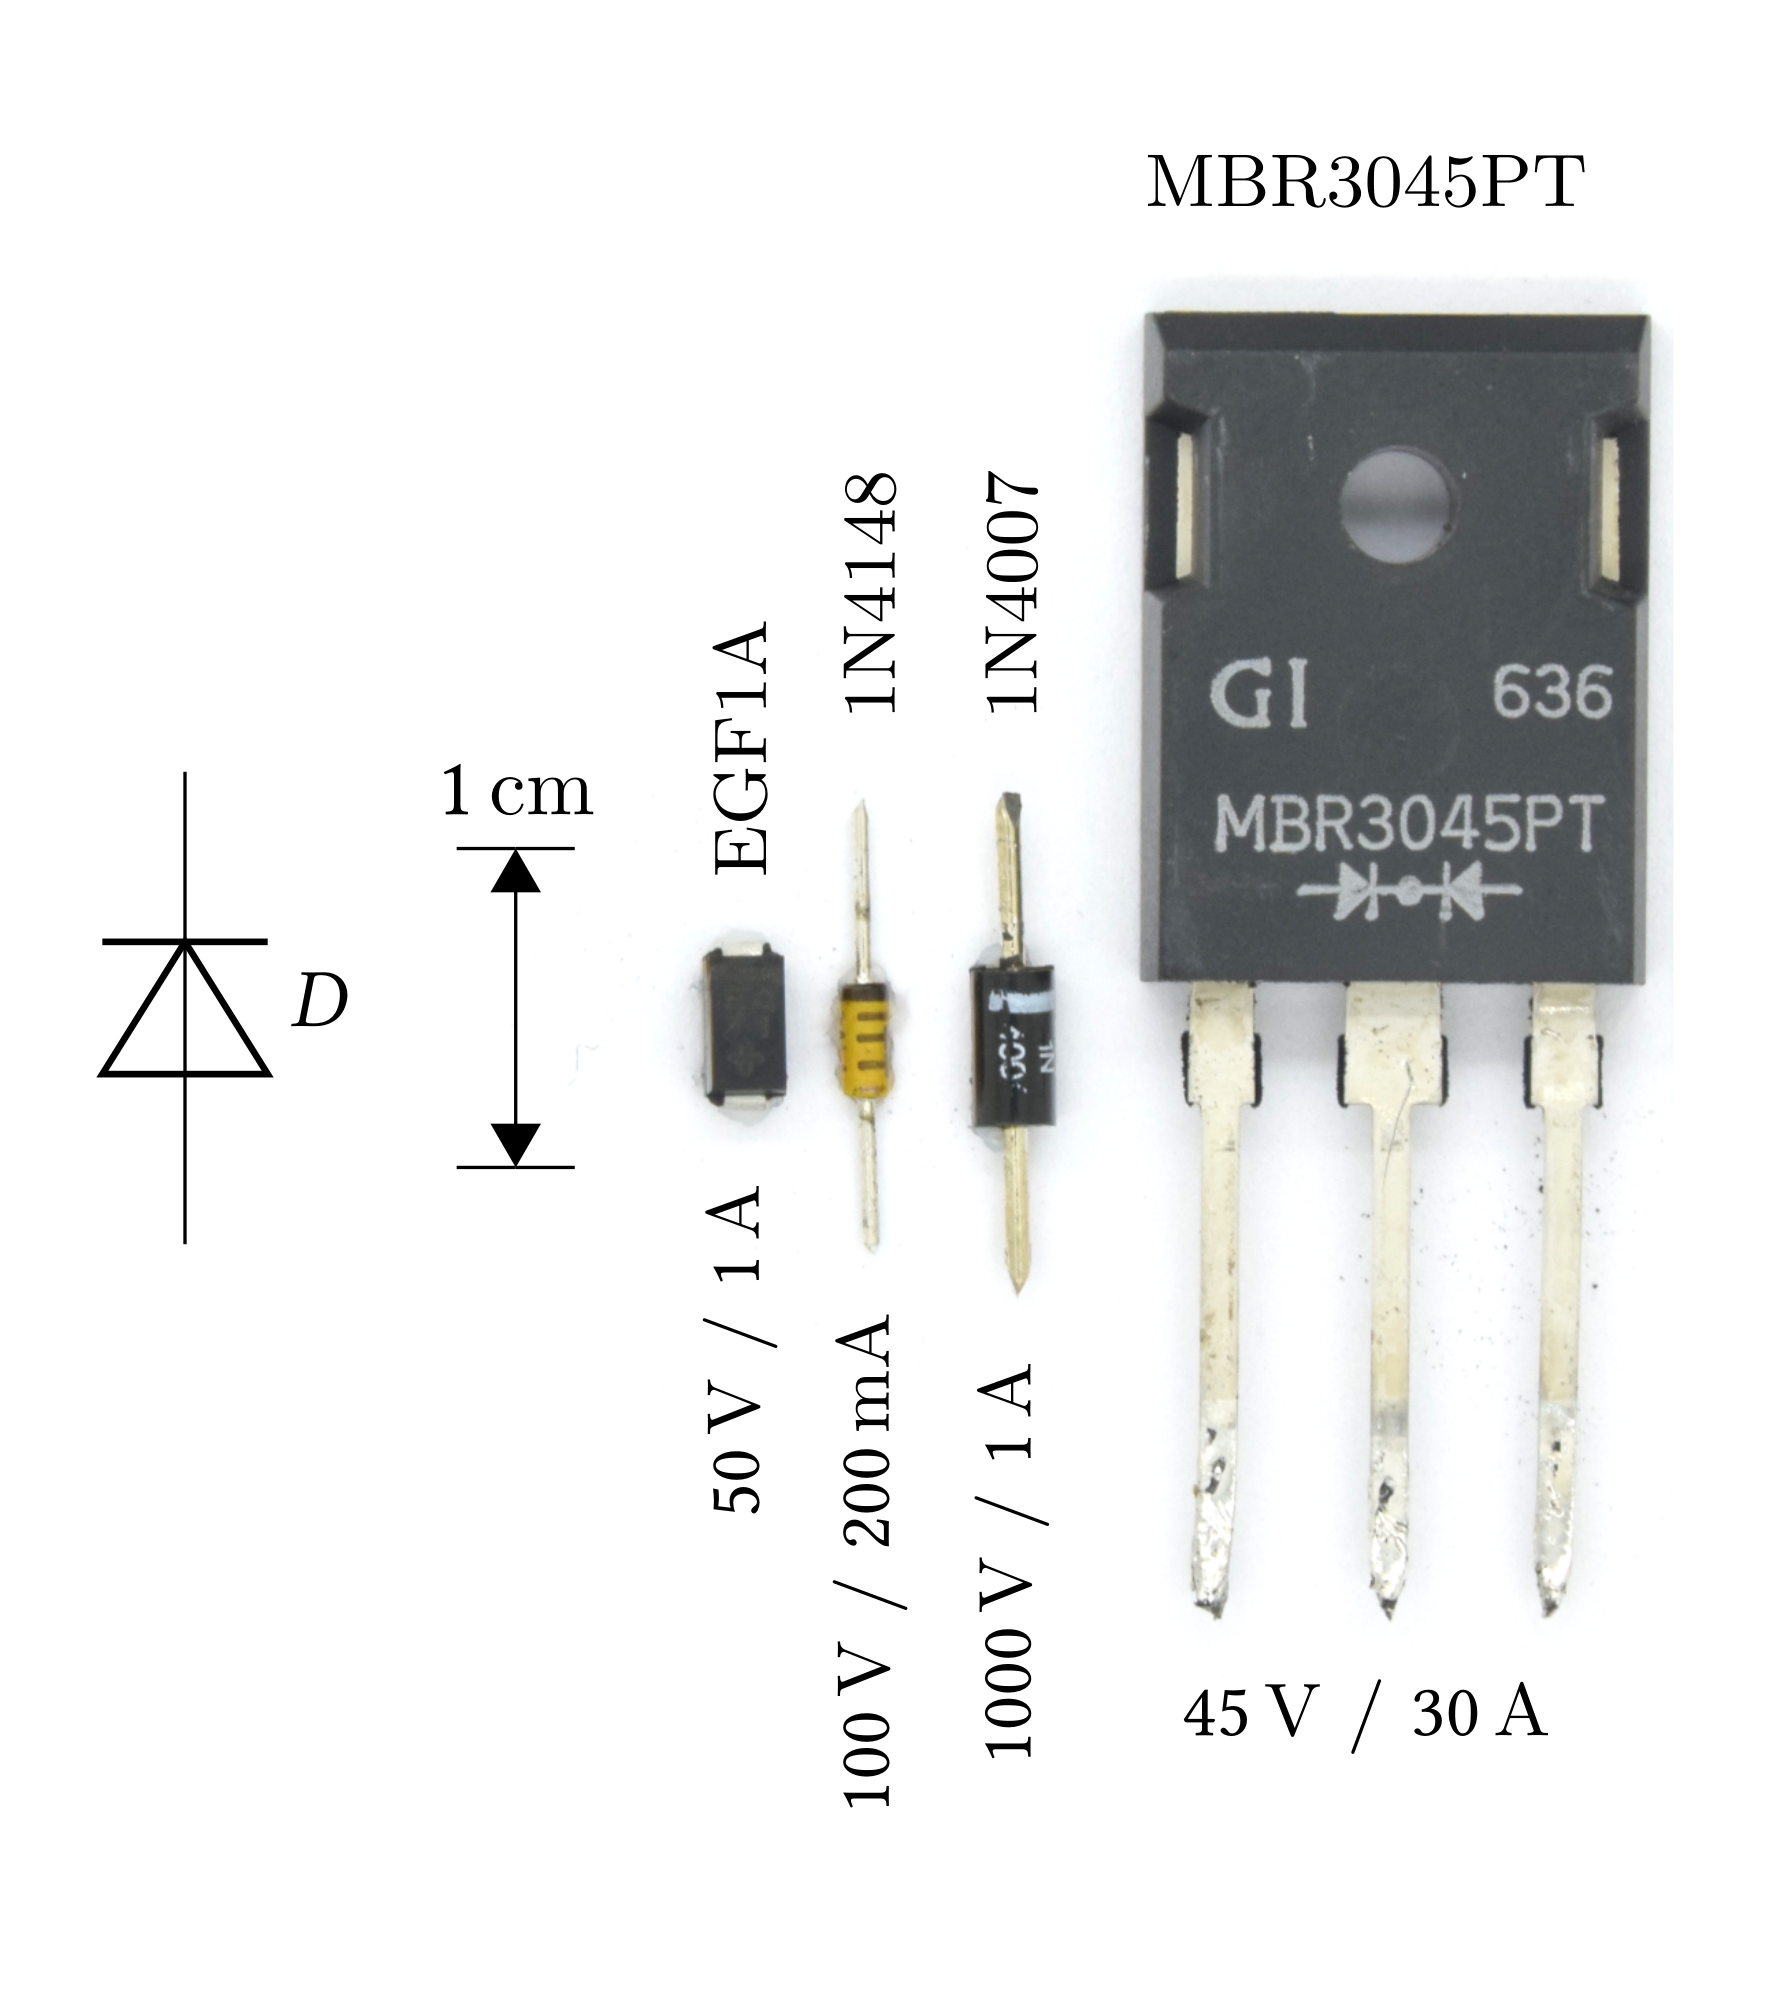
\includegraphics[width=0.85\textwidth]{foto/204}
    \caption{\scriptsize Schaltzeichen und Bauformen von Dioden}
    \label{n_halbleiter_dioden}
\end{figure}

   \end{column}
\end{columns}

\end{frame}

\begin{frame}
\only<1>{
\begin{PQuestion}{NC401}{Welches Bauteil wird durch das Schaltzeichen symbolisiert?}{Spule}
{Widerstand}
{Diode}
{Kondensator}
{\DARCimage{0.5\linewidth}{381include}}\end{PQuestion}

}
\only<2>{
\begin{PQuestion}{NC401}{Welches Bauteil wird durch das Schaltzeichen symbolisiert?}{Spule}
{Widerstand}
{\textbf{\textcolor{DARCgreen}{Diode}}}
{Kondensator}
{\DARCimage{0.5\linewidth}{381include}}\end{PQuestion}

}
\end{frame}

\begin{frame}
\frametitle{Anschlüsse einer Diode}
\begin{columns}
    \begin{column}{0.48\textwidth}
    \begin{itemize}
  \item Anode und Kathode
  \item Plus-Pol an Anode und Minus-Pol an Kathode: \emph{Diode leitet}
  \item Plus-Pol an Kathode und Minus-Pol an Anode: \emph{Diode sperrt}
  \end{itemize}

    \end{column}
   \begin{column}{0.48\textwidth}
       
\begin{figure}
    \DARCimage{0.85\linewidth}{666include}
    \caption{\scriptsize Merkhilfe Diode}
    \label{n_halbleiter_diode_merkhilfe}
\end{figure}


   \end{column}
\end{columns}

\end{frame}

\begin{frame}
\only<1>{
\begin{PQuestion}{NC403}{Wie lauten die Bezeichnungen für die Anschlüsse 1 und 2 im Schaltsymbol?}{1 = Anode; 2 = Kathode}
{1 = Kathode; 2 = Anode}
{1 = Basis; 2 = Kathode}
{1 = Emitter; 2 = Anode}
{\DARCimage{0.5\linewidth}{383include}}\end{PQuestion}

}
\only<2>{
\begin{PQuestion}{NC403}{Wie lauten die Bezeichnungen für die Anschlüsse 1 und 2 im Schaltsymbol?}{\textbf{\textcolor{DARCgreen}{1 = Anode; 2 = Kathode}}}
{1 = Kathode; 2 = Anode}
{1 = Basis; 2 = Kathode}
{1 = Emitter; 2 = Anode}
{\DARCimage{0.5\linewidth}{383include}}\end{PQuestion}

}
\end{frame}

\begin{frame}
\only<1>{
\begin{question2x2}{NC404}{In welchem der abgebildeten Stromkreise fließt Strom?}{\DARCimage{0.75\linewidth}{520include}}
{\DARCimage{0.75\linewidth}{519include}}
{\DARCimage{0.75\linewidth}{518include}}
{\DARCimage{0.75\linewidth}{521include}}
\end{question2x2}

}
\only<2>{
\begin{question2x2}{NC404}{In welchem der abgebildeten Stromkreise fließt Strom?}{\DARCimage{0.75\linewidth}{520include}}
{\DARCimage{0.75\linewidth}{519include}}
{\textbf{\textcolor{DARCgreen}{\DARCimage{0.75\linewidth}{518include}}}}
{\DARCimage{0.75\linewidth}{521include}}
\end{question2x2}

}
\end{frame}

\begin{frame}
\frametitle{LED}
\begin{columns}
    \begin{column}{0.48\textwidth}
    \begin{itemize}
  \item Leuchtdiode, \enquote{light-emitting diode}
  \item Leuchtet, sobald Strom durch sie hindurchfließt
  \item Schaltbild: Diode mit zwei zusätzlichen Pfeilen nach außen
  \item Verhält sich wie Diode, aber leuchtet
  \end{itemize}

    \end{column}
   \begin{column}{0.48\textwidth}
       
\begin{figure}
    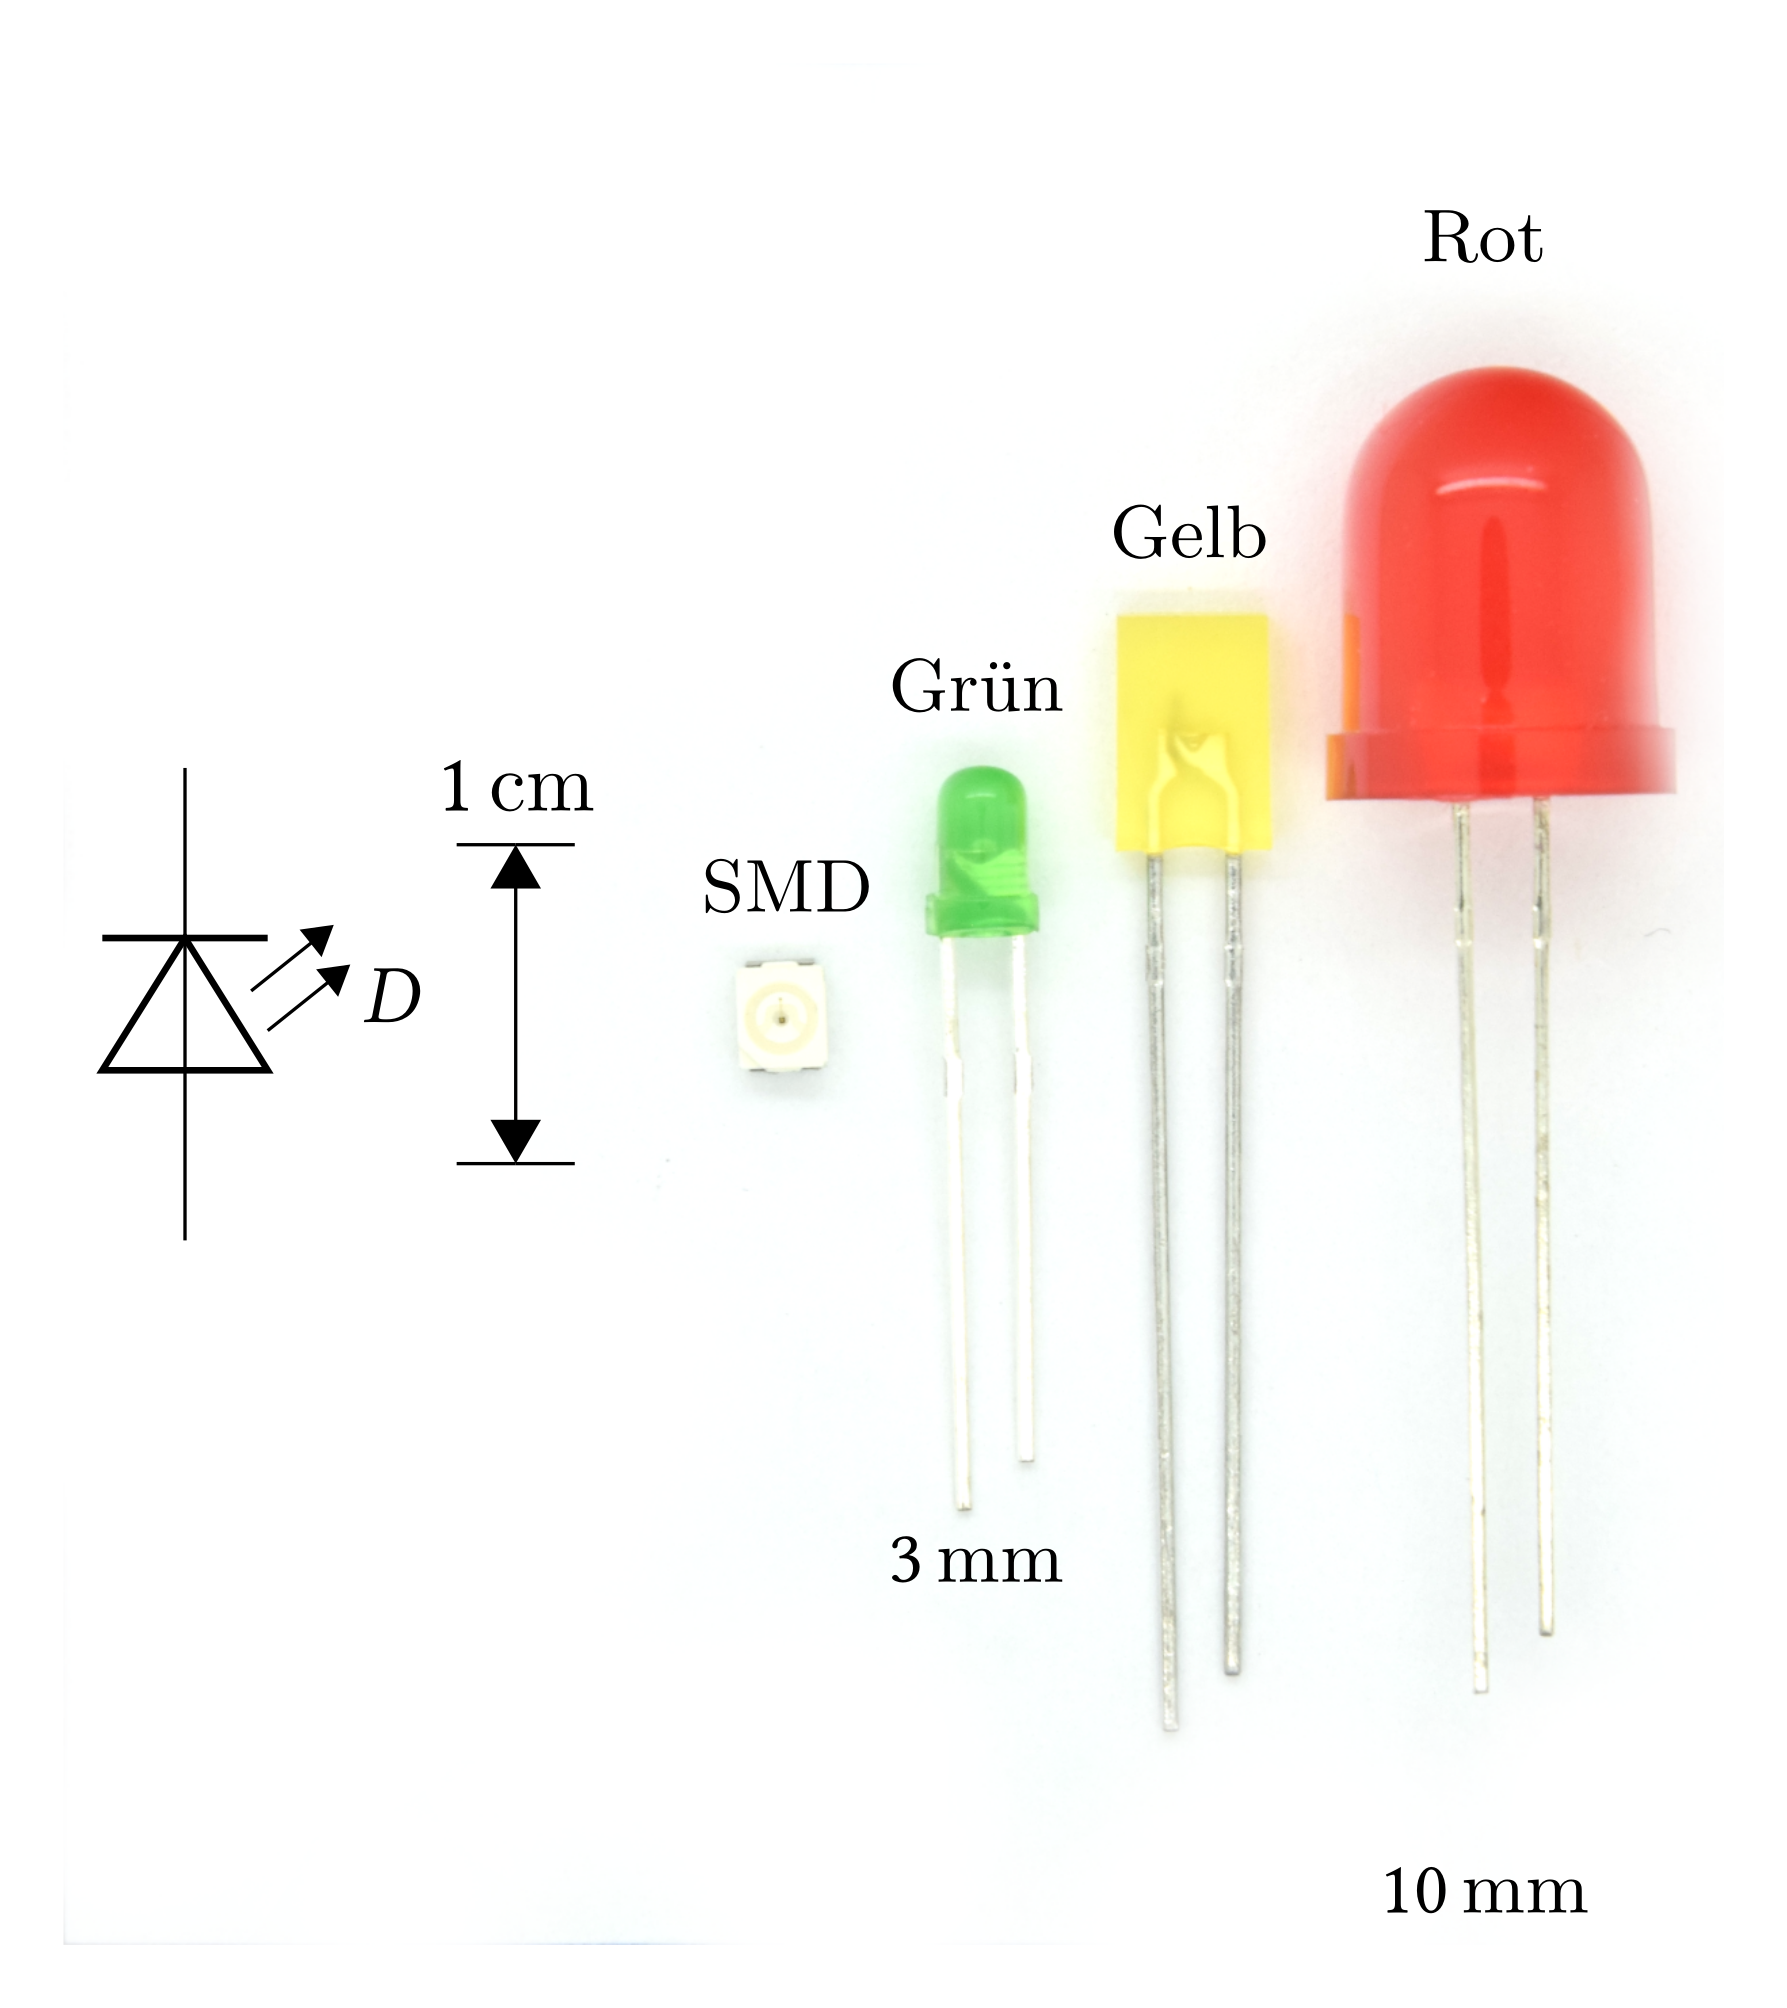
\includegraphics[width=0.85\textwidth]{foto/205}
    \caption{\scriptsize Schaltzeichen und Bauformen von LEDs}
    \label{n_halbleiter_led}
\end{figure}

   \end{column}
\end{columns}

\end{frame}

\begin{frame}
\only<1>{
\begin{PQuestion}{NC402}{Welches Bauteil wird durch das Schaltzeichen symbolisiert?}{Batterie}
{Spule}
{Kondensator}
{Leuchtdiode}
{\DARCimage{0.5\linewidth}{522include}}\end{PQuestion}

}
\only<2>{
\begin{PQuestion}{NC402}{Welches Bauteil wird durch das Schaltzeichen symbolisiert?}{Batterie}
{Spule}
{Kondensator}
{\textbf{\textcolor{DARCgreen}{Leuchtdiode}}}
{\DARCimage{0.5\linewidth}{522include}}\end{PQuestion}

}
\end{frame}

\begin{frame}
\only<1>{
\begin{question2x2}{NB703}{Bei welchem der abgebildeten Stromkreise leuchtet die LED?}{\DARCimage{0.75\linewidth}{513include}}
{\DARCimage{0.75\linewidth}{514include}}
{\DARCimage{0.75\linewidth}{515include}}
{\DARCimage{0.75\linewidth}{516include}}
\end{question2x2}

}
\only<2>{
\begin{question2x2}{NB703}{Bei welchem der abgebildeten Stromkreise leuchtet die LED?}{\textbf{\textcolor{DARCgreen}{\DARCimage{0.75\linewidth}{513include}}}}
{\DARCimage{0.75\linewidth}{514include}}
{\DARCimage{0.75\linewidth}{515include}}
{\DARCimage{0.75\linewidth}{516include}}
\end{question2x2}

}
\end{frame}%ENDCONTENT


\section{Leistung}
\label{section:leistung}
\begin{frame}%STARTCONTENT
\begin{itemize}
  \item Elektrische Geräte haben eine Leistungsaufnahme angegeben
  \item Beispiele: LED-Leuchtmittel 7 W, Staubsauger 425 W
  \item An jedem Widerstand wird elektrische Leistung umgesetzt
  \item Strom fließt durch einen Widerstand $\rightarrow$ Umwandlung von elektrischer Energie in thermische Energie
  \item Je größer der Strom, desto mehr Wärme
  \end{itemize}
\end{frame}

\begin{frame}
\only<1>{
\begin{QQuestion}{NA204}{Welche Einheit wird üblicherweise für die elektrische Leistung verwendet?}{Kilowattstunden (kWh)}
{Watt (W)}
{Joule (J)}
{Amperestunden (Ah)}
\end{QQuestion}

}
\only<2>{
\begin{QQuestion}{NA204}{Welche Einheit wird üblicherweise für die elektrische Leistung verwendet?}{Kilowattstunden (kWh)}
{\textbf{\textcolor{DARCgreen}{Watt (W)}}}
{Joule (J)}
{Amperestunden (Ah)}
\end{QQuestion}

}
\end{frame}

\begin{frame}
\only<1>{
\begin{QQuestion}{NA211}{\qty{0,010}{\W} entspricht ...}{\qty{10}{\mW}}
{\qty{10}{\micro\W}}
{\qty{100}{\nano\W}}
{\qty{100}{\pico\W}}
\end{QQuestion}

}
\only<2>{
\begin{QQuestion}{NA211}{\qty{0,010}{\W} entspricht ...}{\textbf{\textcolor{DARCgreen}{\qty{10}{\mW}}}}
{\qty{10}{\micro\W}}
{\qty{100}{\nano\W}}
{\qty{100}{\pico\W}}
\end{QQuestion}

}
\end{frame}

\begin{frame}
\only<1>{
\begin{QQuestion}{NA210}{\qty{1}{\W} entspricht ...}{\qty{1000}{\micro\W}}
{\qty{1000}{\mW}}
{\qty{1000}{\nano\W}}
{\qty{1000}{\pico\W}}
\end{QQuestion}

}
\only<2>{
\begin{QQuestion}{NA210}{\qty{1}{\W} entspricht ...}{\qty{1000}{\micro\W}}
{\textbf{\textcolor{DARCgreen}{\qty{1000}{\mW}}}}
{\qty{1000}{\nano\W}}
{\qty{1000}{\pico\W}}
\end{QQuestion}

}
\end{frame}

\begin{frame}
\frametitle{Berechnung der Leistung}
Abhängig von Strom und Spannung

$ P = U \cdot I $

$ U = \dfrac{P}{I} $

$ I = \dfrac{P}{U} $

\end{frame}

\begin{frame}
\only<1>{
\begin{QQuestion}{NB601}{Welche Leistung nimmt ein Transceiver bei \qty{13,8}{\V} Gleichspannung auf, wenn das Strommessgerät im Netzteil \qty{1,5}{\A} anzeigt?}{\qty{9,2}{\W}}
{\qty{1,53}{\W}}
{\qty{2,07}{\W}}
{\qty{20,7}{\W}}
\end{QQuestion}

}
\only<2>{
\begin{QQuestion}{NB601}{Welche Leistung nimmt ein Transceiver bei \qty{13,8}{\V} Gleichspannung auf, wenn das Strommessgerät im Netzteil \qty{1,5}{\A} anzeigt?}{\qty{9,2}{\W}}
{\qty{1,53}{\W}}
{\qty{2,07}{\W}}
{\textbf{\textcolor{DARCgreen}{\qty{20,7}{\W}}}}
\end{QQuestion}

}
\end{frame}

\begin{frame}
\only<1>{
\begin{QQuestion}{NB602}{An einem Vorwiderstand fällt bei einem Strom von \qty{50}{\mA} eine Spannung von \qty{50}{\V} ab. Wieviel Leistung wird an diesem in Wärme umgesetzt?}{\qty{2,5}{\W}}
{\qty{1}{\kW}}
{\qty{1}{\W}}
{\qty{250}{\mW}}
\end{QQuestion}

}
\only<2>{
\begin{QQuestion}{NB602}{An einem Vorwiderstand fällt bei einem Strom von \qty{50}{\mA} eine Spannung von \qty{50}{\V} ab. Wieviel Leistung wird an diesem in Wärme umgesetzt?}{\textbf{\textcolor{DARCgreen}{\qty{2,5}{\W}}}}
{\qty{1}{\kW}}
{\qty{1}{\W}}
{\qty{250}{\mW}}
\end{QQuestion}

}
\end{frame}

\begin{frame}
\only<1>{
\begin{QQuestion}{NB603}{An einem Vorwiderstand fällt bei einem Strom von \qty{20}{\mA} eine Spannung von \qty{3,2}{\V} ab. Wieviel Leistung wird an diesem in Wärme umgesetzt?}{\qty{64,0}{\mW}}
{\qty{0,16}{\mW}}
{\qty{6,25}{\mW}}
{\qty{20}{\mW}}
\end{QQuestion}

}
\only<2>{
\begin{QQuestion}{NB603}{An einem Vorwiderstand fällt bei einem Strom von \qty{20}{\mA} eine Spannung von \qty{3,2}{\V} ab. Wieviel Leistung wird an diesem in Wärme umgesetzt?}{\textbf{\textcolor{DARCgreen}{\qty{64,0}{\mW}}}}
{\qty{0,16}{\mW}}
{\qty{6,25}{\mW}}
{\qty{20}{\mW}}
\end{QQuestion}

}
\end{frame}

\begin{frame}
\only<1>{
\begin{QQuestion}{NB606}{Ein gleichspannungsbetriebenes Leuchtmittel ist mit der Angabe \qty{12}{\V} / \qty{48}{\W} bedruckt.  Bei einer \qty{12}{\V}-Versorgung beträgt die Stromentnahme~...}{\qty{4}{\A}.}
{\qty{250}{\mA}.}
{\qty{750}{\mA}.}
{\qty{36}{\A}.}
\end{QQuestion}

}
\only<2>{
\begin{QQuestion}{NB606}{Ein gleichspannungsbetriebenes Leuchtmittel ist mit der Angabe \qty{12}{\V} / \qty{48}{\W} bedruckt.  Bei einer \qty{12}{\V}-Versorgung beträgt die Stromentnahme~...}{\textbf{\textcolor{DARCgreen}{\qty{4}{\A}.}}}
{\qty{250}{\mA}.}
{\qty{750}{\mA}.}
{\qty{36}{\A}.}
\end{QQuestion}

}
\end{frame}

\begin{frame}
\only<1>{
\begin{QQuestion}{NB604}{Ein Mobil-Transceiver (Sendeempfänger) wird aus dem Bordnetz eines Kraftfahrzeuges mit \qty{12}{\V}~Nennspannung betrieben und hat bei Sendebetrieb eine Leistungsaufnahme von \qty{100}{\W}. Wie groß ist dann die Stromaufnahme?}{\qty{0,12}{\A}}
{\qty{16,6}{\A}}
{\qty{1200}{\A}}
{\qty{8,33}{\A}}
\end{QQuestion}

}
\only<2>{
\begin{QQuestion}{NB604}{Ein Mobil-Transceiver (Sendeempfänger) wird aus dem Bordnetz eines Kraftfahrzeuges mit \qty{12}{\V}~Nennspannung betrieben und hat bei Sendebetrieb eine Leistungsaufnahme von \qty{100}{\W}. Wie groß ist dann die Stromaufnahme?}{\qty{0,12}{\A}}
{\qty{16,6}{\A}}
{\qty{1200}{\A}}
{\textbf{\textcolor{DARCgreen}{\qty{8,33}{\A}}}}
\end{QQuestion}

}
 \end{frame}

\begin{frame}
\only<1>{
\begin{QQuestion}{NB605}{Ein Leuchtmittel hat einen Nennwert von \qty{12}{\V} und \qty{3}{\W}. Wie viel Strom fließt beim Anschluss an \qty{12}{\V}?}{\qty{2,5}{\A}}
{\qty{400}{\mA}}
{\qty{4}{\A}}
{\qty{250}{\mA}}
\end{QQuestion}

}
\only<2>{
\begin{QQuestion}{NB605}{Ein Leuchtmittel hat einen Nennwert von \qty{12}{\V} und \qty{3}{\W}. Wie viel Strom fließt beim Anschluss an \qty{12}{\V}?}{\qty{2,5}{\A}}
{\qty{400}{\mA}}
{\qty{4}{\A}}
{\textbf{\textcolor{DARCgreen}{\qty{250}{\mA}}}}
\end{QQuestion}

}
\end{frame}%ENDCONTENT


\section{Leistung beim Wechselstrom}
\label{section:wechselstrom_leistung}
\begin{frame}%STARTCONTENT
\begin{itemize}
  \item Berechnung mit Effektivwert
  \item $U_{\textrm{eff}} = \frac{\^{U}}{\sqrt{2}}$
  \item $I_{\textrm{eff}} = \frac{\^{I}}{\sqrt{2}}$
  \end{itemize}
\end{frame}

\begin{frame}
\only<1>{
\begin{QQuestion}{AB301}{Ein sinusförmiger Wechselstrom mit einer Amplitude $I_{\symup{max}}$ von 0,5 Ampere fließt durch einen Widerstand von \qty{20}{\ohm}. Wieviel Leistung wird in Wärme umgesetzt?}{\qty{3,5}{\W}}
{\qty{5,0}{\W}}
{\qty{10}{\W}}
{\qty{2,5}{\W}}
\end{QQuestion}

}
\only<2>{
\begin{QQuestion}{AB301}{Ein sinusförmiger Wechselstrom mit einer Amplitude $I_{\symup{max}}$ von 0,5 Ampere fließt durch einen Widerstand von \qty{20}{\ohm}. Wieviel Leistung wird in Wärme umgesetzt?}{\qty{3,5}{\W}}
{\qty{5,0}{\W}}
{\qty{10}{\W}}
{\textbf{\textcolor{DARCgreen}{\qty{2,5}{\W}}}}
\end{QQuestion}

}
\end{frame}

\begin{frame}
\frametitle{Lösungsweg}
\begin{itemize}
  \item gegeben: $I_{\textrm{max}} = 0,5A$
  \item gegeben: $R = 20\Omega$
  \item gesucht: $P$
  \end{itemize}
    \pause
    \begin{equation}\begin{split} \nonumber P &=  I^2 \cdot R = (\frac{I_{\textrm{max}}}{\sqrt{2}})^2 \cdot R\\ &= \frac{(0,5A)^2}{2} \cdot 20\Omega \\ &= \frac{1}{8}A^2 \cdot 20\Omega = 2,5W \end{split}\end{equation}



\end{frame}%ENDCONTENT


\section{Leistung II}
\label{section:leistung_2}
\begin{frame}%STARTCONTENT

\frametitle{Leistungsberechnung}
Wir kennen bereits

$P = U\cdot I = \dfrac{U^2}{R} = I^2\cdot R$
\begin{columns}
    \begin{column}{0.48\textwidth}
    Nach U umgestellt:

$U = \dfrac{P}{I} = \sqrt{P \cdot R}$


    \end{column}
   \begin{column}{0.48\textwidth}
       Nach I umgestellt:

$I = \dfrac{P}{U} = \sqrt{\dfrac{P}{R}}$


   \end{column}
\end{columns}

\end{frame}

\begin{frame}
\only<1>{
\begin{QQuestion}{EB505}{In welcher Antwort sind alle dargestellten Zusammenhänge zwischen Strom, Spannung, Widerstand und Leistung richtig?}{$I = \dfrac{\sqrt{P}}{R};\quad U = \sqrt{P}\cdot R$}
{$I = \sqrt{P\cdot R};\quad U = \sqrt{\dfrac{P}{R}}$}
{$I = \sqrt{\dfrac{R}{P}};\quad U = \sqrt{P\cdot R}$}
{$I = \sqrt{\dfrac{P}{R}};\quad U = \sqrt{P\cdot R}$}
\end{QQuestion}

}
\only<2>{
\begin{QQuestion}{EB505}{In welcher Antwort sind alle dargestellten Zusammenhänge zwischen Strom, Spannung, Widerstand und Leistung richtig?}{$I = \dfrac{\sqrt{P}}{R};\quad U = \sqrt{P}\cdot R$}
{$I = \sqrt{P\cdot R};\quad U = \sqrt{\dfrac{P}{R}}$}
{$I = \sqrt{\dfrac{R}{P}};\quad U = \sqrt{P\cdot R}$}
{\textbf{\textcolor{DARCgreen}{$I = \sqrt{\dfrac{P}{R}};\quad U = \sqrt{P\cdot R}$}}}
\end{QQuestion}

}
\end{frame}

\begin{frame}
\only<1>{
\begin{QQuestion}{EB506}{In welcher Antwort sind alle dargestellten Zusammenhänge zwischen Widerstand, Leistung, Spannung und Strom richtig?}{$R = \dfrac{U^2}{P};\quad R = \dfrac{P}{I^2}$}
{$R = U^2\cdot I;\quad R = \dfrac{P}{I^2}$}
{$R = \dfrac{P}{U^2};\quad R = P\cdot I^2$}
{$R = \dfrac{U^2}{P};\quad R = P\cdot I^2$}
\end{QQuestion}

}
\only<2>{
\begin{QQuestion}{EB506}{In welcher Antwort sind alle dargestellten Zusammenhänge zwischen Widerstand, Leistung, Spannung und Strom richtig?}{\textbf{\textcolor{DARCgreen}{$R = \dfrac{U^2}{P};\quad R = \dfrac{P}{I^2}$}}}
{$R = U^2\cdot I;\quad R = \dfrac{P}{I^2}$}
{$R = \dfrac{P}{U^2};\quad R = P\cdot I^2$}
{$R = \dfrac{U^2}{P};\quad R = P\cdot I^2$}
\end{QQuestion}

}
\end{frame}

\begin{frame}
\only<1>{
\begin{QQuestion}{EB504}{An einem Widerstand $R$ wird die elektrische Leistung $P$ in Wärme umgesetzt. Sie kennen die Größen $P$ und $R$. Nach welcher der Formeln können Sie die Spannung ermitteln, die an dem Widerstand $R$ anliegt?}{$U = \dfrac{P}{R}$}
{$U = R\cdot P$}
{$U = \sqrt{\dfrac{P}{R}}$}
{$U = \sqrt{P\cdot R}$}
\end{QQuestion}

}
\only<2>{
\begin{QQuestion}{EB504}{An einem Widerstand $R$ wird die elektrische Leistung $P$ in Wärme umgesetzt. Sie kennen die Größen $P$ und $R$. Nach welcher der Formeln können Sie die Spannung ermitteln, die an dem Widerstand $R$ anliegt?}{$U = \dfrac{P}{R}$}
{$U = R\cdot P$}
{$U = \sqrt{\dfrac{P}{R}}$}
{\textbf{\textcolor{DARCgreen}{$U = \sqrt{P\cdot R}$}}}
\end{QQuestion}

}
\end{frame}

\begin{frame}
\only<1>{
\begin{QQuestion}{EB507}{Der Effektivwert der Spannung an einer künstlichen \qty{50}{\ohm}-Antenne wird mit \qty{100}{\V} gemessen. Die Leistung an der Last beträgt~...}{\qty{100}{\W}.}
{\qty{50}{\W}.}
{\qty{200}{\W}.}
{\qty{400}{\W}.}
\end{QQuestion}

}
\only<2>{
\begin{QQuestion}{EB507}{Der Effektivwert der Spannung an einer künstlichen \qty{50}{\ohm}-Antenne wird mit \qty{100}{\V} gemessen. Die Leistung an der Last beträgt~...}{\qty{100}{\W}.}
{\qty{50}{\W}.}
{\textbf{\textcolor{DARCgreen}{\qty{200}{\W}.}}}
{\qty{400}{\W}.}
\end{QQuestion}

}
\end{frame}

\begin{frame}
\only<1>{
\begin{QQuestion}{EB508}{Wieviel Leistung wird an einer künstlichen \qty{50}{\ohm}-Antenne umgesetzt, wenn ein effektiver Strom von \qty{2}{\A} fließt?}{\qty{25}{\W}}
{\qty{100}{\W}}
{\qty{200}{\W}}
{\qty{250}{\W}}
\end{QQuestion}

}
\only<2>{
\begin{QQuestion}{EB508}{Wieviel Leistung wird an einer künstlichen \qty{50}{\ohm}-Antenne umgesetzt, wenn ein effektiver Strom von \qty{2}{\A} fließt?}{\qty{25}{\W}}
{\qty{100}{\W}}
{\textbf{\textcolor{DARCgreen}{\qty{200}{\W}}}}
{\qty{250}{\W}}
\end{QQuestion}

}
\end{frame}

\begin{frame}
\only<1>{
\begin{QQuestion}{EB509}{Für welche Leistung muss ein \qty{100}{\ohm}-Widerstand mindestens ausgelegt sein, wenn an ihm \qty{10}{\V} abfallen sollen?}{\qty{10,0}{\W}}
{\qty{1,00}{\W}}
{\qty{0,01}{\W}}
{\qty{0,10}{\W}}
\end{QQuestion}

}
\only<2>{
\begin{QQuestion}{EB509}{Für welche Leistung muss ein \qty{100}{\ohm}-Widerstand mindestens ausgelegt sein, wenn an ihm \qty{10}{\V} abfallen sollen?}{\qty{10,0}{\W}}
{\textbf{\textcolor{DARCgreen}{\qty{1,00}{\W}}}}
{\qty{0,01}{\W}}
{\qty{0,10}{\W}}
\end{QQuestion}

}
\end{frame}

\begin{frame}
\only<1>{
\begin{QQuestion}{EB510}{Ein Widerstand von \qty{10}{\kohm} hat eine maximale Spannungsfestigkeit von \qty{700}{\V} und eine maximale Belastbarkeit von \qty{1}{\W}. Welche Gleichspannung darf höchstens an den Widerstand angelegt werden, um ihn im spezifizierten Bereich zu betreiben?}{\qty{775}{\V}}
{\qty{0,01}{\kV}}
{\qty{0,7}{\kV}}
{\qty{100}{\V}}
\end{QQuestion}

}
\only<2>{
\begin{QQuestion}{EB510}{Ein Widerstand von \qty{10}{\kohm} hat eine maximale Spannungsfestigkeit von \qty{700}{\V} und eine maximale Belastbarkeit von \qty{1}{\W}. Welche Gleichspannung darf höchstens an den Widerstand angelegt werden, um ihn im spezifizierten Bereich zu betreiben?}{\qty{775}{\V}}
{\qty{0,01}{\kV}}
{\qty{0,7}{\kV}}
{\textbf{\textcolor{DARCgreen}{\qty{100}{\V}}}}
\end{QQuestion}

}
\end{frame}

\begin{frame}
\only<1>{
\begin{QQuestion}{EB511}{Ein Widerstand von \qty{100}{\kohm} hat eine maximale Spannungsfestigkeit von \qty{1000}{\V} und eine maximale Belastbarkeit von \qty{6}{\W}. Welche Gleichspannung darf höchstens an den Widerstand angelegt werden ohne ihn zu überlasten?}{\qty{100}{\V}}
{\qty{775}{\V}}
{\qty{0,07}{\kV}}
{\qty{1,00}{\kV}}
\end{QQuestion}

}
\only<2>{
\begin{QQuestion}{EB511}{Ein Widerstand von \qty{100}{\kohm} hat eine maximale Spannungsfestigkeit von \qty{1000}{\V} und eine maximale Belastbarkeit von \qty{6}{\W}. Welche Gleichspannung darf höchstens an den Widerstand angelegt werden ohne ihn zu überlasten?}{\qty{100}{\V}}
{\textbf{\textcolor{DARCgreen}{\qty{775}{\V}}}}
{\qty{0,07}{\kV}}
{\qty{1,00}{\kV}}
\end{QQuestion}

}
\end{frame}

\begin{frame}
\only<1>{
\begin{QQuestion}{EB512}{Ein Widerstand von \qty{120}{\ohm} hat eine Belastbarkeit von \qty{23,0}{\W}. Welcher Strom darf höchstens durch den Widerstand fließen, damit er nicht überlastet wird?}{\qty{2,28}{\A}}
{\qty{192}{\mA}}
{\qty{43,7}{\mA}}
{\qty{438}{\mA}}
\end{QQuestion}

}
\only<2>{
\begin{QQuestion}{EB512}{Ein Widerstand von \qty{120}{\ohm} hat eine Belastbarkeit von \qty{23,0}{\W}. Welcher Strom darf höchstens durch den Widerstand fließen, damit er nicht überlastet wird?}{\qty{2,28}{\A}}
{\qty{192}{\mA}}
{\qty{43,7}{\mA}}
{\textbf{\textcolor{DARCgreen}{\qty{438}{\mA}}}}
\end{QQuestion}

}
\end{frame}

\begin{frame}
\frametitle{Leistung bei Wechselspannung}
\begin{itemize}
  \item Bei Wechselspannungen muss mit dem Effektivwert gerechnet werden
  \end{itemize}
\end{frame}

\begin{frame}
\only<1>{
\begin{QQuestion}{EB503}{Gelten die Formeln für die Leistung an einem rein ohmschen Widerstand auch bei Wechselspannung?}{Nein, da die periodische Änderung von Strom und Spannung dann vernachlässigt wird.}
{Ja, wenn mit den Effektivwerten gerechnet wird.}
{Ja, wenn mit den Spitzenwerten gerechnet wird.}
{Nein, da die Blindleistung nicht berücksichtigt wird.}
\end{QQuestion}

}
\only<2>{
\begin{QQuestion}{EB503}{Gelten die Formeln für die Leistung an einem rein ohmschen Widerstand auch bei Wechselspannung?}{Nein, da die periodische Änderung von Strom und Spannung dann vernachlässigt wird.}
{\textbf{\textcolor{DARCgreen}{Ja, wenn mit den Effektivwerten gerechnet wird.}}}
{Ja, wenn mit den Spitzenwerten gerechnet wird.}
{Nein, da die Blindleistung nicht berücksichtigt wird.}
\end{QQuestion}

}
\end{frame}

\begin{frame}
\only<1>{
\begin{QQuestion}{EB513}{Ein Oszilloskop zeigt einen sinusförmigen Spitze-Spitze-Wert von \qty{25}{\V} an einem \qty{1000}{\ohm} Widerstand an. Der Effektivstrom durch den Widerstand beträgt~...}{\qty{25}{\mA}.}
{\qty{12,5}{\mA}.}
{\qty{8,8}{\mA}.}
{\qty{40}{\A}.}
\end{QQuestion}

}
\only<2>{
\begin{QQuestion}{EB513}{Ein Oszilloskop zeigt einen sinusförmigen Spitze-Spitze-Wert von \qty{25}{\V} an einem \qty{1000}{\ohm} Widerstand an. Der Effektivstrom durch den Widerstand beträgt~...}{\qty{25}{\mA}.}
{\qty{12,5}{\mA}.}
{\textbf{\textcolor{DARCgreen}{\qty{8,8}{\mA}.}}}
{\qty{40}{\A}.}
\end{QQuestion}

}

\end{frame}

\begin{frame}
\frametitle{PEP}
\begin{itemize}
  \item \emph{Peak Envelope Power} ist die Spitzenleistung eines Senders
  \item Leistung bei der höchsten Spitze einer Hochfrequenzschwingung
  \end{itemize}

\end{frame}

\begin{frame}
\only<1>{
\begin{QQuestion}{EB501}{Die Spitzenleistung eines Senders (PEP) ist~...}{die unmittelbar nach dem Senderausgang messbare Leistung über die Spitzen der Periode einer durchschnittlichen Hochfrequenzschwingung, bevor Zusatzgeräte (z.~B. Anpassgeräte) durchlaufen werden.}
{die Leistung, die der Sender unter normalen Betriebsbedingungen während einer Periode der Hochfrequenzschwingung bei der höchsten Spitze der Modulationshüllkurve durchschnittlich an einen reellen Abschlusswiderstand abgeben kann.}
{die durchschnittliche Leistung, die ein Sender unter normalen Betriebsbedingungen an die Antennenspeiseleitung während eines Zeitintervalls abgibt, das im Verhältnis zur Periode der tiefsten Modulationsfrequenz ausreichend lang ist.}
{das Produkt aus der Leistung, die unmittelbar der Antenne zugeführt wird, und ihrem Gewinnfaktor in einer Richtung, bezogen auf den Halbwellendipol.}
\end{QQuestion}

}
\only<2>{
\begin{QQuestion}{EB501}{Die Spitzenleistung eines Senders (PEP) ist~...}{die unmittelbar nach dem Senderausgang messbare Leistung über die Spitzen der Periode einer durchschnittlichen Hochfrequenzschwingung, bevor Zusatzgeräte (z.~B. Anpassgeräte) durchlaufen werden.}
{\textbf{\textcolor{DARCgreen}{die Leistung, die der Sender unter normalen Betriebsbedingungen während einer Periode der Hochfrequenzschwingung bei der höchsten Spitze der Modulationshüllkurve durchschnittlich an einen reellen Abschlusswiderstand abgeben kann.}}}
{die durchschnittliche Leistung, die ein Sender unter normalen Betriebsbedingungen an die Antennenspeiseleitung während eines Zeitintervalls abgibt, das im Verhältnis zur Periode der tiefsten Modulationsfrequenz ausreichend lang ist.}
{das Produkt aus der Leistung, die unmittelbar der Antenne zugeführt wird, und ihrem Gewinnfaktor in einer Richtung, bezogen auf den Halbwellendipol.}
\end{QQuestion}

}
\end{frame}

\begin{frame}
\frametitle{Mittlere Leistung}
\begin{itemize}
  \item Durchschnittliche Leistung eines Senders
  \item Beschreibung ergibt zu einem späteren Zeitpunkt mehr Sinn, wenn Hüllkurven durchgesprochen wurden
  \end{itemize}
\end{frame}

\begin{frame}
\only<1>{
\begin{QQuestion}{EB502}{Die mittlere Leistung eines Senders ist~...}{das Produkt aus der Leistung, die unmittelbar der Antenne zugeführt wird, und ihrem Gewinnfaktor in einer Richtung, bezogen auf den Halbwellendipol.}
{die unmittelbar nach dem Senderausgang messbare Leistung über die Spitzen der Periode einer durchschnittlichen Hochfrequenzschwingung, bevor Zusatzgeräte (z.~B. Anpassgeräte) durchlaufen werden.}
{die durchschnittliche Leistung, die ein Sender unter normalen Betriebsbedingungen während einer Periode der Hochfrequenzschwingung bei der höchsten Spitze der Modulationshüllkurve der Antennenspeiseleitung zuführt.}
{die durchschnittliche Leistung, die ein Sender unter normalen Betriebsbedingungen an die Antennenspeiseleitung während eines Zeitintervalls abgibt, das im Verhältnis zur Periode der tiefsten Modulationsfrequenz ausreichend lang ist.}
\end{QQuestion}

}
\only<2>{
\begin{QQuestion}{EB502}{Die mittlere Leistung eines Senders ist~...}{das Produkt aus der Leistung, die unmittelbar der Antenne zugeführt wird, und ihrem Gewinnfaktor in einer Richtung, bezogen auf den Halbwellendipol.}
{die unmittelbar nach dem Senderausgang messbare Leistung über die Spitzen der Periode einer durchschnittlichen Hochfrequenzschwingung, bevor Zusatzgeräte (z.~B. Anpassgeräte) durchlaufen werden.}
{die durchschnittliche Leistung, die ein Sender unter normalen Betriebsbedingungen während einer Periode der Hochfrequenzschwingung bei der höchsten Spitze der Modulationshüllkurve der Antennenspeiseleitung zuführt.}
{\textbf{\textcolor{DARCgreen}{die durchschnittliche Leistung, die ein Sender unter normalen Betriebsbedingungen an die Antennenspeiseleitung während eines Zeitintervalls abgibt, das im Verhältnis zur Periode der tiefsten Modulationsfrequenz ausreichend lang ist.}}}
\end{QQuestion}

}
\end{frame}%ENDCONTENT


\section{Dezibel I}
\label{section:dezibel_1}
\begin{frame}%STARTCONTENT

\frametitle{Dezibel einfach erklärt}
\begin{table}
\begin{DARCtabular}{lr}
    Was  &Leistung in mW   \\
     effektive Leistung EME-Station  & 100 000 000   \\
     Standard Transceiver  & 100 000   \\
     Kleine Handfunke  & 1 000   \\
     Lautsprechersignal (Zimmerlautstärke)  & 100   \\
     Kopfhörersignal  & 1   \\
     Lautes KW-Signal  & 0,000 001   \\
     Leises KW-Signal (Antenneneingang RX)  & 0,000 000 000 001   \\
\end{DARCtabular}
\caption{Leistungen in mW}
\label{e_dezibel_leistungen_mw}
\end{table}
Wer mit diesen Zahlen umgeht, fängt automatisch an, die Nullen zu zählen.

\end{frame}

\begin{frame}Wir zählen die Nullen (und nennen das Ergebnis \enquote{Bel})

\begin{table}
\begin{DARCtabular}{lrr}
    Was  &Leistung in mW  &Bel   \\
     effektive Leistung EME-Station  & 100 000 000  & 8   \\
     Standard Transceiver  & 100 000  & 5   \\
     Kleine Handfunke  & 1 000  & 3   \\
     Lautsprechersignal (Zimmerlautstärke)  & 100  & 2   \\
     Kopfhörersignal  & 1  & 0   \\
     Lautes KW-Signal  & 0,000 001  & -6   \\
     Leises KW-Signal (Antenneneingang RX)  & 0,000 000 000 001  & -12   \\
\end{DARCtabular}
\caption{Leistungen in mW und Bel}
\label{e_dezibel_leistungen_bel}
\end{table}

\end{frame}

\begin{frame}dBm = Dezibel bezogen auf mW

\begin{table}
\begin{DARCtabular}{lrrr}
    Was  &Leistung in mW  &Bel  &dBm   \\
     effektive Leistung EME-Station  & 100 000 000  & 8  & 80   \\
     Standard Transceiver  & 100 000  & 5  & 50   \\
     Kleine Handfunke  & 1 000  & 3  & 30   \\
     Lautsprechersignal (Zimmerlautstärke)  & 100  & 2  & 20   \\
     Kopfhörersignal  & 1  & 0  & 0   \\
     Lautes KW-Signal  & 0,000 001  & -6  & -60   \\
     Leises KW-Signal (Antenneneingang RX)  & 0,000 000 000 001  & -12  & -120   \\
\end{DARCtabular}
\caption{Leistungen in mW und Bel}
\label{e_dezibel_leistungen_bel}
\end{table}

\end{frame}

\begin{frame}
\frametitle{Leistungsverstärkung}
\emph{Empfänger}

\begin{itemize}
  \item Eingangssignal: 0,000 000 000 \qty{001}{\milli\watt}
  \item Ausgangssignal: \qty{100}{\milli\watt}
  \item Benötigte Verstärkung: 100 000 000 000 000
  \end{itemize}
\emph{Sender}

\begin{itemize}
  \item Frequenzerzeugende Stufe (Oszillator): \qty{10}{\milli\watt}
  \item Ausgangssignal: 100 \qty{000}{\milli\watt}
  \item Benötigte Verstärkung: 10 000
  \end{itemize}
\end{frame}

\begin{frame}
\frametitle{Leistungsverstärkung mit dB}
\emph{Empfänger}

\begin{itemize}
  \item Eingangssignal: 0,000 000 000 \qty{001}{\milli\watt} = -\qty{120}{\dBm}
  \item Ausgangssignal: \qty{100}{\milli\watt} = \qty{20}{\dBm}
  \item Benötigte Verstärkung: 100 000 000 000 000 = \qty{140}{\dB}
  \end{itemize}
\emph{Sender}

\begin{itemize}
  \item Frequenzerzeugende Stufe (Oszillator): \qty{10}{\milli\watt} = \qty{10}{\dBm}
  \item Ausgangssignal: 100 \qty{000}{\milli\watt} = \qty{50}{\dBm}
  \item Benötigte Verstärkung: 10 000 = \qty{40}{\dB}
  \end{itemize}

\end{frame}

\begin{frame}
\frametitle{Wichtige Leistungsfaktoren}
\begin{table}
\begin{DARCtabular}{cc}
    dB  & $\approx$  Leistungsfaktor   \\
     0  & 1   \\
     1,5  &$\sqrt{2} = 1,41$  \\
     2,15  & 1,64   \\
     3  & 2   \\
     5  &$\sqrt{10} = 3,16$  \\
     6  & 4   \\
     10  & 10   \\
     20  & 100   \\
\end{DARCtabular}
\caption{Wichtige Leistungsfaktoren in dB}
\label{e_dezibel_leistungsfaktoren}
\end{table}

\end{frame}

\begin{frame}
\frametitle{Berechnung mit Taschenrechner}
Ältere Modelle

\begin{itemize}
  \item Faktor-Wert $\rightarrow$ \emph{log}-Taste $\rightarrow$ $\cdot$10 $\rightarrow$ dB
  \item dB-Wert $\rightarrow$  $\div$ 10 $\rightarrow$ \emph{10<sup>x</sup>}-Taste $\rightarrow$ Faktor
  \end{itemize}
Neuere Modelle

\begin{itemize}
  \item \emph{log}-Taste $\rightarrow$ Faktor-Wert $\rightarrow$ \emph{)}-Taste $\rightarrow$ $\cdot$10 $\rightarrow$ \emph{=}-Taste $\rightarrow$ dB
  \item \emph{10<sup>x</sup>}-Taste $\rightarrow$ dB-Wert $\rightarrow$  $\div$ 10 $\rightarrow$ \emph{=}-Taste $\rightarrow$ Faktor
  \end{itemize}
\end{frame}

\begin{frame}
\only<1>{
\begin{QQuestion}{EA107}{Um wie viel Dezibel verändert sich der Leistungspegel, wenn die Leistung verdoppelt wird?}{\qty{3}{\decibel}}
{\qty{6}{\decibel}}
{\qty{1,5}{\decibel}}
{\qty{12}{\decibel}}
\end{QQuestion}

}
\only<2>{
\begin{QQuestion}{EA107}{Um wie viel Dezibel verändert sich der Leistungspegel, wenn die Leistung verdoppelt wird?}{\textbf{\textcolor{DARCgreen}{\qty{3}{\decibel}}}}
{\qty{6}{\decibel}}
{\qty{1,5}{\decibel}}
{\qty{12}{\decibel}}
\end{QQuestion}

}
\end{frame}%ENDCONTENT


\section{Dezibel II}
\label{section:dezibel_2}
\begin{frame}%STARTCONTENT

\frametitle{Leistungsverhältnis}
Faktor 10

$p = 10\cdot \log_{10}(\frac{P}{1mW})\textrm{dBm}$

$p = 10\cdot \log_{10}(\frac{P}{1W})\textrm{dBW}$

$0\textrm{dBm}$ liegt bei $P = 1mW$ vor.

$0\textrm{dBW}$ liegt bei $P = 1W$ vor.

\end{frame}

\begin{frame}
\only<1>{
\begin{QQuestion}{AA110}{Welcher Leistung entsprechen die Pegel \qty{0}{\dBm}, \qty{3}{\dBm} und \qty{20}{\dBm}?}{\qty{0}{\mW}, \qty{30}{\mW}, \qty{200}{\mW}}
{\qty{1}{\mW}, \qty{1,4}{\mW}, \qty{10}{\mW}}
{\qty{1}{\mW}, \qty{2}{\mW}, \qty{100}{\mW}}
{\qty{0}{\mW}, \qty{3}{\mW}, \qty{20}{\mW}}
\end{QQuestion}

}
\only<2>{
\begin{QQuestion}{AA110}{Welcher Leistung entsprechen die Pegel \qty{0}{\dBm}, \qty{3}{\dBm} und \qty{20}{\dBm}?}{\qty{0}{\mW}, \qty{30}{\mW}, \qty{200}{\mW}}
{\qty{1}{\mW}, \qty{1,4}{\mW}, \qty{10}{\mW}}
{\textbf{\textcolor{DARCgreen}{\qty{1}{\mW}, \qty{2}{\mW}, \qty{100}{\mW}}}}
{\qty{0}{\mW}, \qty{3}{\mW}, \qty{20}{\mW}}
\end{QQuestion}

}
\end{frame}

\begin{frame}
\only<1>{
\begin{QQuestion}{AA105}{Einer Leistungsverstärkung von 40 entsprechen~...}{\qty{32}{\decibel}.}
{\qty{36,8}{\decibel}.}
{\qty{16}{\decibel}.}
{\qty{73,8}{\decibel}.}
\end{QQuestion}

}
\only<2>{
\begin{QQuestion}{AA105}{Einer Leistungsverstärkung von 40 entsprechen~...}{\qty{32}{\decibel}.}
{\qty{36,8}{\decibel}.}
{\textbf{\textcolor{DARCgreen}{\qty{16}{\decibel}.}}}
{\qty{73,8}{\decibel}.}
\end{QQuestion}

}
\end{frame}

\begin{frame}
\frametitle{Spannungsverhältnis}
Faktor 20

$u = 20\cdot \log_{10}(\frac{U}{0,775V})\textrm{dBu}$

$0\textrm{dBu}$ liegt bei $U = 0,775V$ vor.

$0\textrm{dBV}$ liegt bei $U = 1V$ vor.

$0\textrm{dBµV}$ liegt bei $U = 1µV$ vor.

\end{frame}

\begin{frame}
\only<1>{
\begin{QQuestion}{AA111}{Einem Spannungsverhältnis von 15 entsprechen~...}{\qty{54}{\decibel}.}
{\qty{15}{\decibel}.}
{\qty{23,5}{\decibel}.}
{\qty{11,7}{\decibel}.}
\end{QQuestion}

}
\only<2>{
\begin{QQuestion}{AA111}{Einem Spannungsverhältnis von 15 entsprechen~...}{\qty{54}{\decibel}.}
{\qty{15}{\decibel}.}
{\textbf{\textcolor{DARCgreen}{\qty{23,5}{\decibel}.}}}
{\qty{11,7}{\decibel}.}
\end{QQuestion}

}
\end{frame}

\begin{frame}
\frametitle{Berechnungen}
\end{frame}

\begin{frame}
\only<1>{
\begin{QQuestion}{AA108}{Der Ausgangspegel eines Senders beträgt \qty{20}{\dBW}. Dies entspricht einer Ausgangsleistung von~...}{$10^{20}$~W.}
{$10^{0,5}$~W.}
{$10^2$~W.}
{$10^1$~W.}
\end{QQuestion}

}
\only<2>{
\begin{QQuestion}{AA108}{Der Ausgangspegel eines Senders beträgt \qty{20}{\dBW}. Dies entspricht einer Ausgangsleistung von~...}{$10^{20}$~W.}
{$10^{0,5}$~W.}
{\textbf{\textcolor{DARCgreen}{$10^2$~W.}}}
{$10^1$~W.}
\end{QQuestion}

}
\end{frame}

\begin{frame}
\frametitle{Lösungsweg}
\begin{itemize}
  \item gegeben: $p = 20\textrm{dBW}$
  \item gesucht: $P$
  \end{itemize}
    \pause
    \begin{equation}\begin{align} \nonumber p &= 10\cdot \log_{10}(\frac{P}{1W})\textrm{dBW}\\ \nonumber \Rightarrow P &= 10^{\frac{p}{10}} \cdot 1W = 10^{\frac{20\textrm{dBW}}{10}} \cdot 1W = 10^2W \end{align}\end{equation}



\end{frame}

\begin{frame}
\only<1>{
\begin{QQuestion}{AA107}{Ein Sender mit \qty{1}{\W} Ausgangsleistung ist an eine Endstufe mit einer Verstärkung von \qty{10}{\decibel} angeschlossen. Wie groß ist der Ausgangspegel der Endstufe?}{\qty{3}{\dBW}}
{\qty{1}{\dBW}}
{\qty{10}{\dBW}}
{\qty{20}{\dBW}}
\end{QQuestion}

}
\only<2>{
\begin{QQuestion}{AA107}{Ein Sender mit \qty{1}{\W} Ausgangsleistung ist an eine Endstufe mit einer Verstärkung von \qty{10}{\decibel} angeschlossen. Wie groß ist der Ausgangspegel der Endstufe?}{\qty{3}{\dBW}}
{\qty{1}{\dBW}}
{\textbf{\textcolor{DARCgreen}{\qty{10}{\dBW}}}}
{\qty{20}{\dBW}}
\end{QQuestion}

}
\end{frame}

\begin{frame}
\only<1>{
\begin{QQuestion}{AA109}{Ein Sender mit \qty{1}{\W} Ausgangsleistung ist an eine Endstufe mit einer Verstärkung von \qty{10}{\decibel} angeschlossen. Wie groß ist der Ausgangspegel der Endstufe?}{\qty{10}{\dBm}}
{\qty{30}{\dBm}}
{\qty{20}{\dBm}}
{\qty{40}{\dBm}}
\end{QQuestion}

}
\only<2>{
\begin{QQuestion}{AA109}{Ein Sender mit \qty{1}{\W} Ausgangsleistung ist an eine Endstufe mit einer Verstärkung von \qty{10}{\decibel} angeschlossen. Wie groß ist der Ausgangspegel der Endstufe?}{\qty{10}{\dBm}}
{\qty{30}{\dBm}}
{\qty{20}{\dBm}}
{\textbf{\textcolor{DARCgreen}{\qty{40}{\dBm}}}}
\end{QQuestion}

}
\end{frame}

\begin{frame}
\frametitle{Lösungsweg}
1W = 1000mW

\qty{10}{\dB} = Faktor 10

1000mW $\cdot$ 10 = 10000mW = 40dBm

\end{frame}

\begin{frame}
\only<1>{
\begin{QQuestion}{AA106}{Ein HF-Leistungsverstärker hat eine Verstärkung von \qty{16}{\decibel} mit maximal \qty{100}{\W} Ausgangsleistung. Welche HF-Ausgangsleistung ist zu erwarten, wenn der Verstärker mit \qty{1}{\W} HF-Eingangsleistung angesteuert wird?}{\qty{40}{\W}}
{\qty{4}{\W}}
{\qty{16}{\W}}
{\qty{20}{\W}}
\end{QQuestion}

}
\only<2>{
\begin{QQuestion}{AA106}{Ein HF-Leistungsverstärker hat eine Verstärkung von \qty{16}{\decibel} mit maximal \qty{100}{\W} Ausgangsleistung. Welche HF-Ausgangsleistung ist zu erwarten, wenn der Verstärker mit \qty{1}{\W} HF-Eingangsleistung angesteuert wird?}{\textbf{\textcolor{DARCgreen}{\qty{40}{\W}}}}
{\qty{4}{\W}}
{\qty{16}{\W}}
{\qty{20}{\W}}
\end{QQuestion}

}
\end{frame}

\begin{frame}
\frametitle{Lösungsweg}
\begin{itemize}
  \item 16dB = 10dB + 6dB = 10 $\cdot$ 4 = 40
  \item 1W $\cdot$ 40 = 40W
  \end{itemize}
\end{frame}

\begin{frame}
\only<1>{
\begin{QQuestion}{AA112}{Der Pegelwert \qty{120}{\decibel}$\upmu$V/m entspricht einer elektrischen Feldstärke von~...}{\qty{1000}{\kV}/m.}
{\qty{0,78}{\V}/m.}
{\qty{41,6}{\V}/m.}
{\qty{1}{\V}/m.}
\end{QQuestion}

}
\only<2>{
\begin{QQuestion}{AA112}{Der Pegelwert \qty{120}{\decibel}$\upmu$V/m entspricht einer elektrischen Feldstärke von~...}{\qty{1000}{\kV}/m.}
{\qty{0,78}{\V}/m.}
{\qty{41,6}{\V}/m.}
{\textbf{\textcolor{DARCgreen}{\qty{1}{\V}/m.}}}
\end{QQuestion}

}
\end{frame}

\begin{frame}
\frametitle{Lösungsweg}
\begin{itemize}
  \item gegeben: $u = 120\textrm{dBµV}/m$
  \item gesucht: $U$
  \end{itemize}
    \pause
    \begin{equation}\begin{align} \nonumber u &= 20\cdot \log_{10}(\frac{U}{1\textrm{µV}})\textrm{\textrm{dBµV}}\\ \nonumber \Rightarrow U &= 10^{\frac{p}{20}} \cdot 1\textrm{µV} = 10^{\frac{120\textrm{dBµV}/m}{20}} \cdot 1\textrm{µV} = 1V/m \end{align}\end{equation}
    \pause
    In der Literatur ist oft zu finden: 120dBµV = 1V



\end{frame}%ENDCONTENT


\section{Ladung und Energie}
\label{section:ladung_energie}
\begin{frame}%STARTCONTENT

\frametitle{Elektrische Ladung}
Strom über Zeit

$Q = I\cdot t$

in Amperesekunde (As)

\end{frame}

\begin{frame}
\only<1>{
\begin{QQuestion}{AA102}{Welche Einheit wird üblicherweise für die elektrische Ladung verwendet?}{Kilowatt (kW)}
{Amperesekunde (As)}
{Joule (J)}
{Ampere (A)}
\end{QQuestion}

}
\only<2>{
\begin{QQuestion}{AA102}{Welche Einheit wird üblicherweise für die elektrische Ladung verwendet?}{Kilowatt (kW)}
{\textbf{\textcolor{DARCgreen}{Amperesekunde (As)}}}
{Joule (J)}
{Ampere (A)}
\end{QQuestion}

}
\end{frame}

\begin{frame}
\frametitle{Elektrische Energie}
Leistung über Zeit

$W = P\cdot t$

in Joule (J) oder Wattstunden (Wh)

\end{frame}

\begin{frame}
\only<1>{
\begin{QQuestion}{AA103}{Welche Einheit wird üblicherweise für die Energie verwendet?}{Volt (V) bzw. Watt pro Ampere (W/A)}
{Joule (J) bzw. Wattstunden (Wh)}
{Watt (W) bzw. Joule pro Stunde (J/h)}
{Watt (W) bzw. Voltampere (VA)}
\end{QQuestion}

}
\only<2>{
\begin{QQuestion}{AA103}{Welche Einheit wird üblicherweise für die Energie verwendet?}{Volt (V) bzw. Watt pro Ampere (W/A)}
{\textbf{\textcolor{DARCgreen}{Joule (J) bzw. Wattstunden (Wh)}}}
{Watt (W) bzw. Joule pro Stunde (J/h)}
{Watt (W) bzw. Voltampere (VA)}
\end{QQuestion}

}
\end{frame}

\begin{frame}
\only<1>{
\begin{QQuestion}{AB502}{Eine Stromversorgung nimmt bei einer Spannung von \qty{230}{\V} einen Strom von \qty{0,63}{\A} auf. Wieviel Energie wird bei einer Betriebsdauer von 7 Stunden umgesetzt?}{\qty{1,01}{\kWh}}
{\qty{0,14}{\kWh}}
{\qty{2,56}{\kWh}}
{\qty{20,7}{\kWh}}
\end{QQuestion}

}
\only<2>{
\begin{QQuestion}{AB502}{Eine Stromversorgung nimmt bei einer Spannung von \qty{230}{\V} einen Strom von \qty{0,63}{\A} auf. Wieviel Energie wird bei einer Betriebsdauer von 7 Stunden umgesetzt?}{\textbf{\textcolor{DARCgreen}{\qty{1,01}{\kWh}}}}
{\qty{0,14}{\kWh}}
{\qty{2,56}{\kWh}}
{\qty{20,7}{\kWh}}
\end{QQuestion}

}
\end{frame}

\begin{frame}
\frametitle{Lösungweg}
\begin{itemize}
  \item gegeben: $U = 230V$
  \item gegeben: $I = 0,63A$
  \item gegeben: $t = 7h$
  \item gesucht: $W$
  \end{itemize}
    \pause
    \begin{equation} \nonumber W = P\cdot t = U\cdot I\cdot t = 230V\cdot 0,63A\cdot 7h = 1,01kWh \end{equation}



\end{frame}

\begin{frame}
\only<1>{
\begin{PQuestion}{AB503}{Wie viel Energie wird vom Widerstand innerhalb einer Stunde in Wärme umgewandelt?}{\qty{0,5}{\W\hour} bzw. \qty{1800}{\J}}
{\qty{2}{\W\hour} bzw. \qty{7200}{\J}}
{\qty{0,1}{\W\hour} bzw. \qty{360}{\J}}
{\qty{1}{\W\hour} bzw. \qty{3600}{\J}}
{\DARCimage{1.0\linewidth}{556include}}\end{PQuestion}

}
\only<2>{
\begin{PQuestion}{AB503}{Wie viel Energie wird vom Widerstand innerhalb einer Stunde in Wärme umgewandelt?}{\qty{0,5}{\W\hour} bzw. \qty{1800}{\J}}
{\qty{2}{\W\hour} bzw. \qty{7200}{\J}}
{\qty{0,1}{\W\hour} bzw. \qty{360}{\J}}
{\textbf{\textcolor{DARCgreen}{\qty{1}{\W\hour} bzw. \qty{3600}{\J}}}}
{\DARCimage{1.0\linewidth}{556include}}\end{PQuestion}

}
\end{frame}

\begin{frame}
\frametitle{Lösungsweg}
\begin{itemize}
  \item gegeben: $U = 10V$
  \item gegeben: $R = 100\Omega$
  \item gegeben: $t = 1h$
  \item gesucht: $W$
  \end{itemize}
    \pause
    \begin{equation} \nonumber W = P\cdot t = \frac{U^2}{R} \cdot t = \frac{(10V)^2}{100\Omega}\cdot 1h = 1Wh \end{equation}



\end{frame}%ENDCONTENT


\section{Schaltzeichen und Bauelemente}
\label{section:bauelemente}
\begin{frame}%STARTCONTENT
\begin{itemize}
  \item Drei weitere grundlegende Bauteile
  \item Funktionsweise ist Stoff für Klasse~E und A
  \item Für die Prüfung: Schaltzeichen erkennen
  \end{itemize}
\end{frame}

\begin{frame}
\frametitle{Kondensator}
\begin{columns}
    \begin{column}{0.48\textwidth}
    \begin{itemize}
  \item Speichert eine kleine Menge Energie
  \item Besteht oft aus zwei parallelen Platten
  \end{itemize}

    \end{column}
   \begin{column}{0.48\textwidth}
       
\begin{figure}
    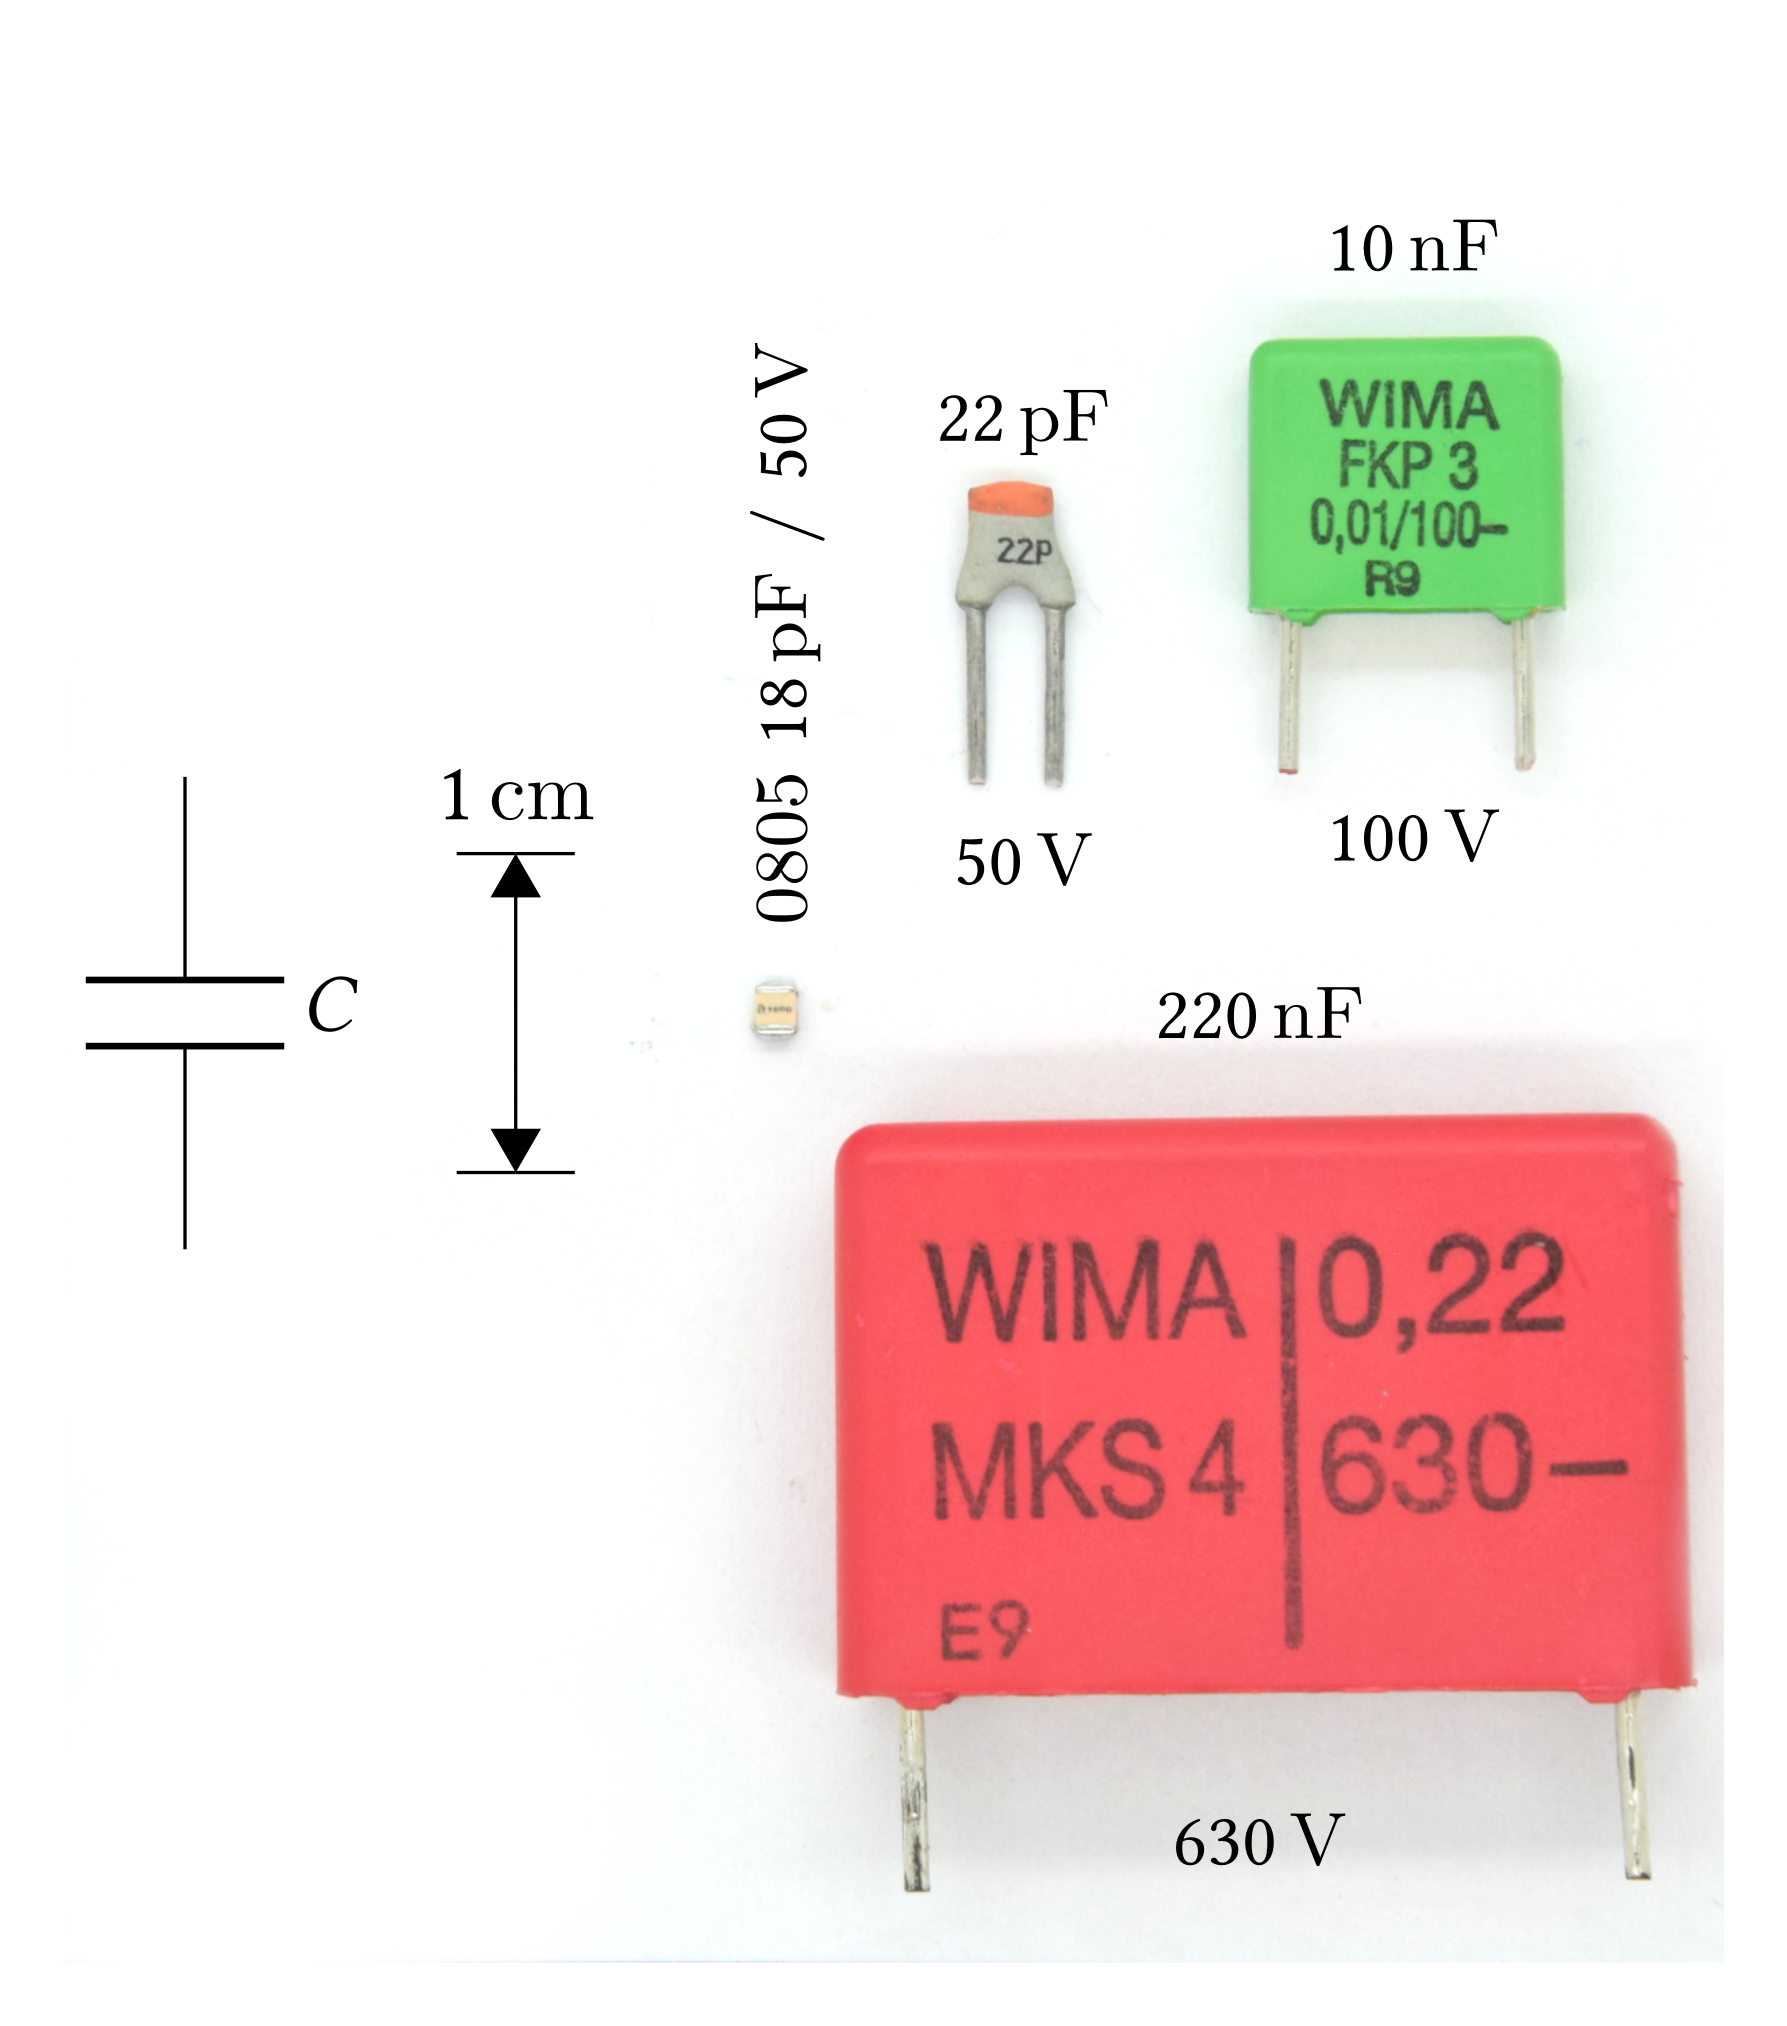
\includegraphics[width=0.85\textwidth]{foto/206}
    \caption{\scriptsize Schaltzeichen und Bauformen von Kondensatoren}
    \label{n_bauelemente_kondensator}
\end{figure}

   \end{column}
\end{columns}

\end{frame}

\begin{frame}
\only<1>{
\begin{PQuestion}{NC201}{Welches Bauteil wird durch das Schaltzeichen symbolisiert?}{Transistor}
{Spule}
{Kondensator}
{Batterie}
{\DARCimage{0.5\linewidth}{511include}}\end{PQuestion}

}
\only<2>{
\begin{PQuestion}{NC201}{Welches Bauteil wird durch das Schaltzeichen symbolisiert?}{Transistor}
{Spule}
{\textbf{\textcolor{DARCgreen}{Kondensator}}}
{Batterie}
{\DARCimage{0.5\linewidth}{511include}}\end{PQuestion}

}
\end{frame}

\begin{frame}
\frametitle{Spule}
\begin{columns}
    \begin{column}{0.48\textwidth}
    \begin{itemize}
  \item Speichert auch eine kleine Menge Energie
  \item Funktioniert technisch aber komplett anders als der Kondensator
  \item Besteht in den einfachen Fällen aus einem aufgewickelten Draht
  \end{itemize}

    \end{column}
   \begin{column}{0.48\textwidth}
       
\begin{figure}
    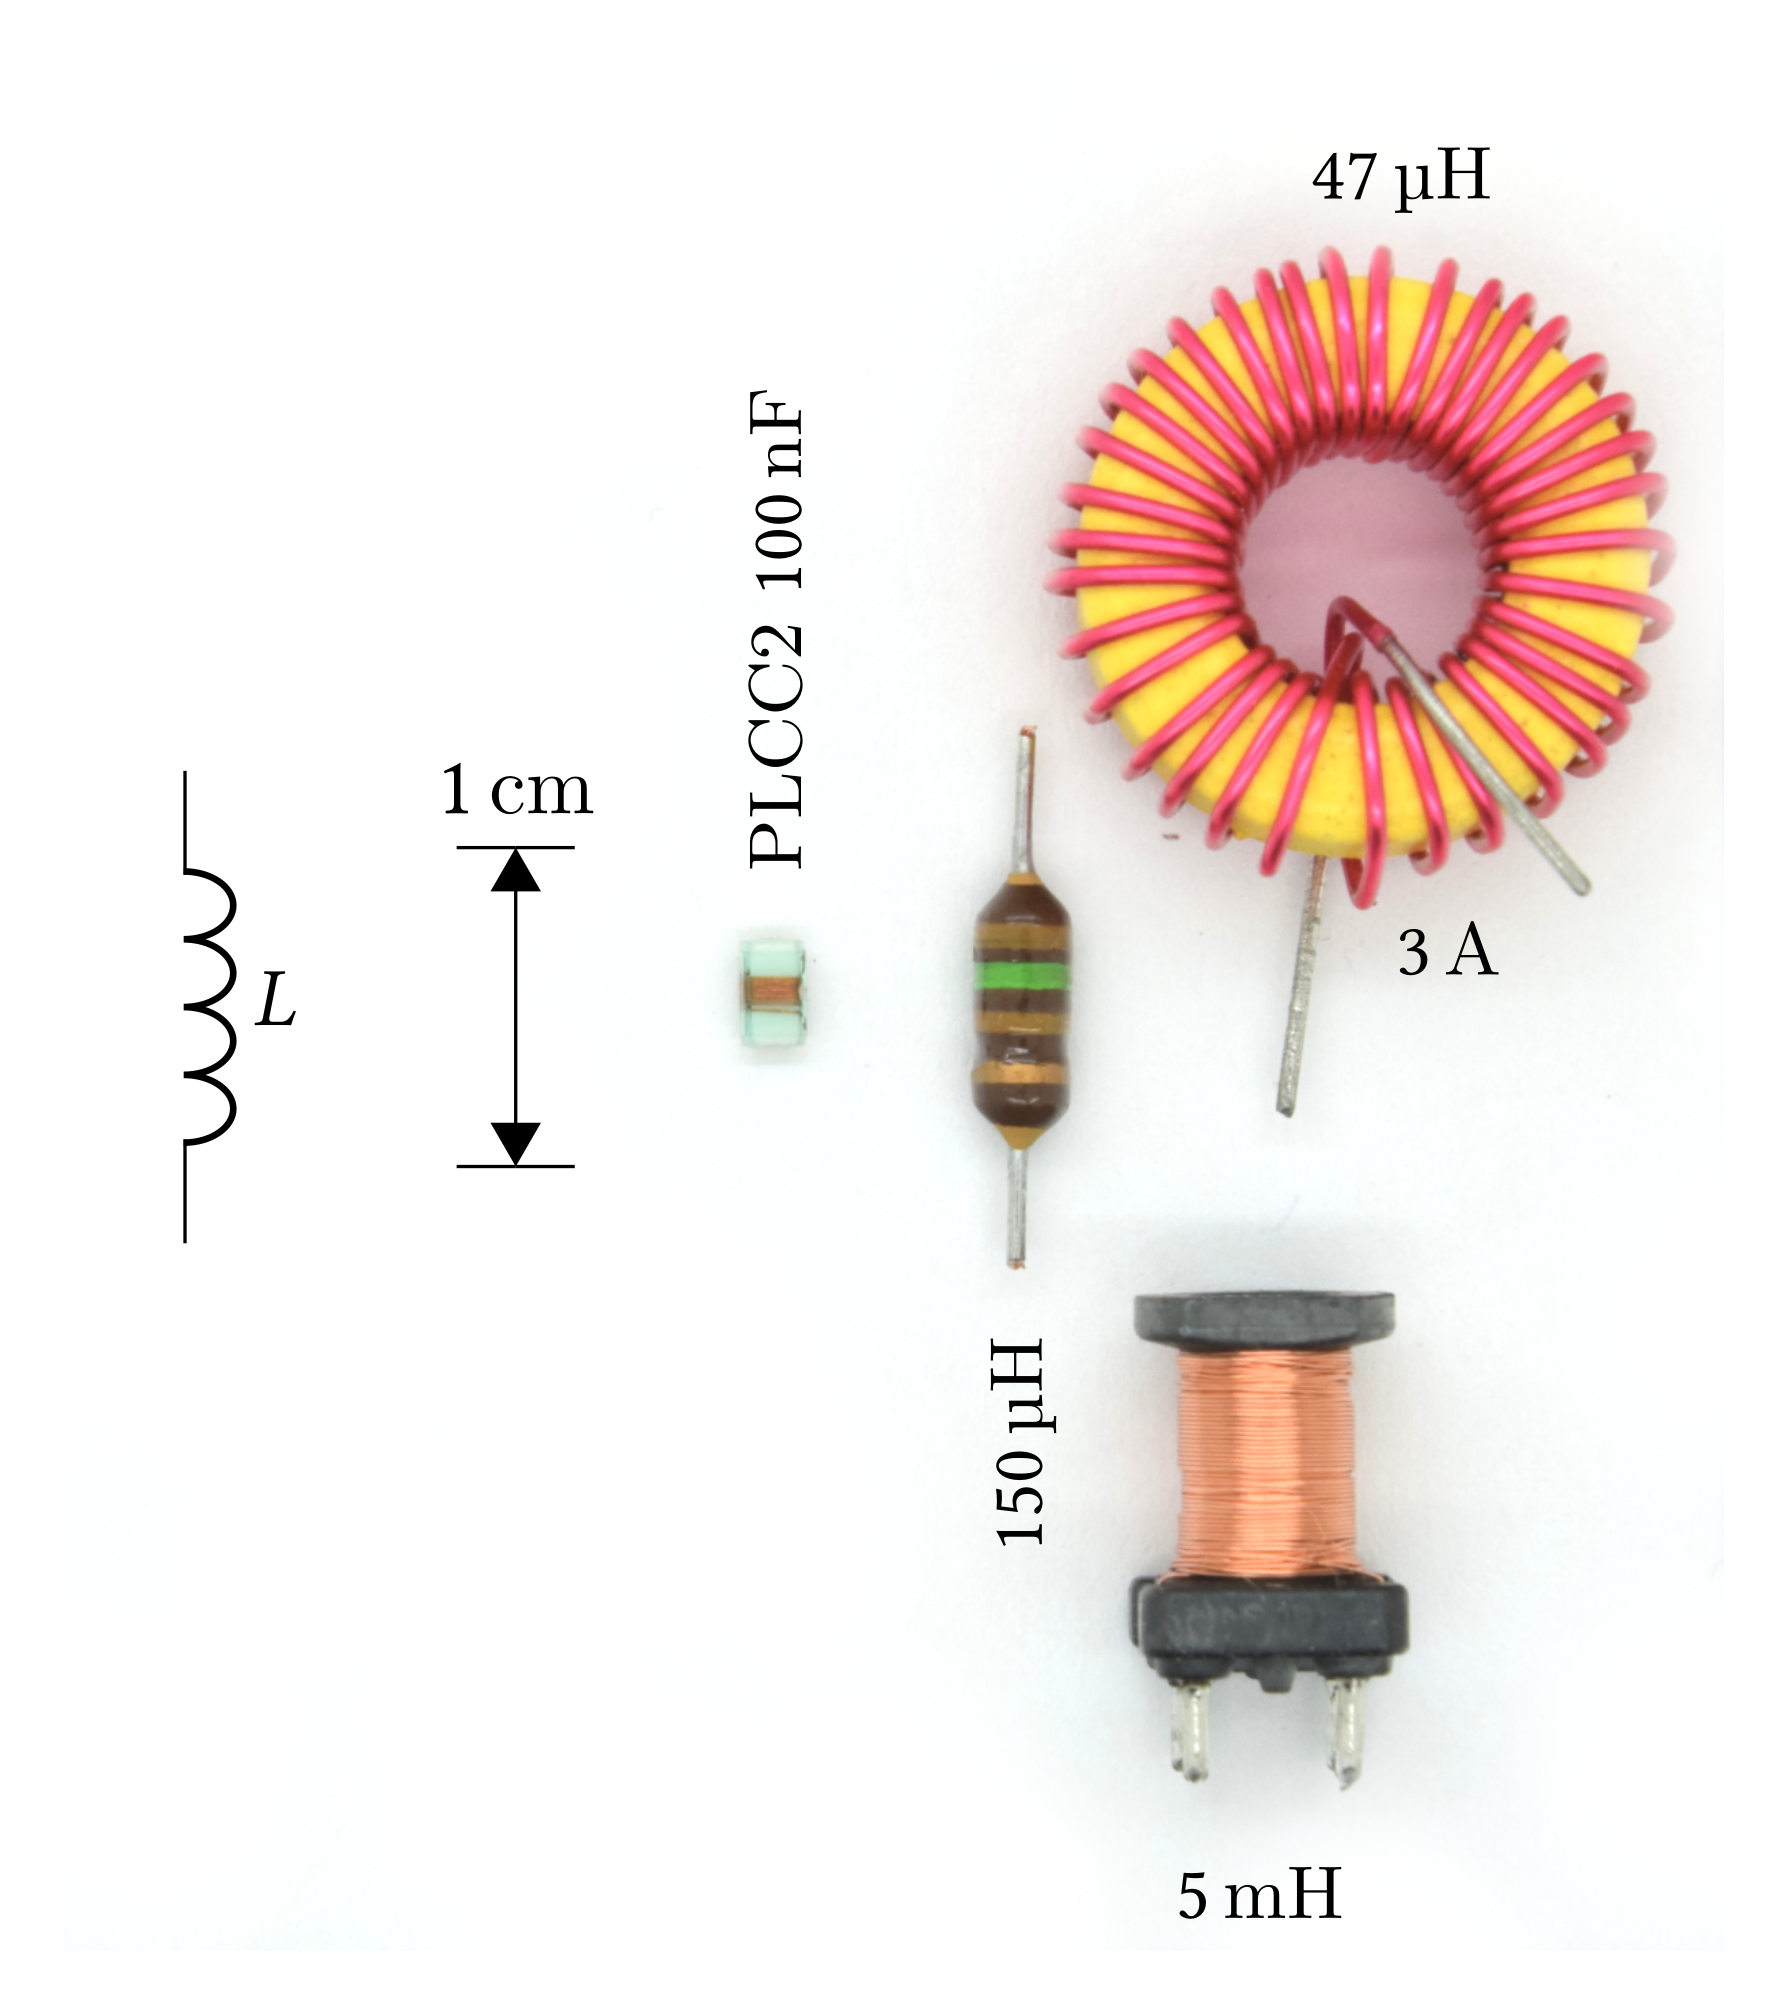
\includegraphics[width=0.85\textwidth]{foto/207}
    \caption{\scriptsize Schaltzeichen und Bauformen von Spulen}
    \label{n_bauelemente_spule}
\end{figure}

   \end{column}
\end{columns}

\end{frame}

\begin{frame}
\only<1>{
\begin{PQuestion}{NC301}{Welches Bauteil wird durch das Schaltzeichen symbolisiert?}{Diode}
{Kondensator}
{Spule}
{Batterie}
{\DARCimage{0.5\linewidth}{512include}}\end{PQuestion}

}
\only<2>{
\begin{PQuestion}{NC301}{Welches Bauteil wird durch das Schaltzeichen symbolisiert?}{Diode}
{Kondensator}
{\textbf{\textcolor{DARCgreen}{Spule}}}
{Batterie}
{\DARCimage{0.5\linewidth}{512include}}\end{PQuestion}

}
\end{frame}

\begin{frame}
\frametitle{Transistor}
\begin{columns}
    \begin{column}{0.48\textwidth}
    \begin{itemize}
  \item Elektrischer Schalter
  \item Oder Verstärker, je nach Beschaltung
  \item Hat drei Anschlüsse
  \end{itemize}

    \end{column}
   \begin{column}{0.48\textwidth}
       
\begin{figure}
    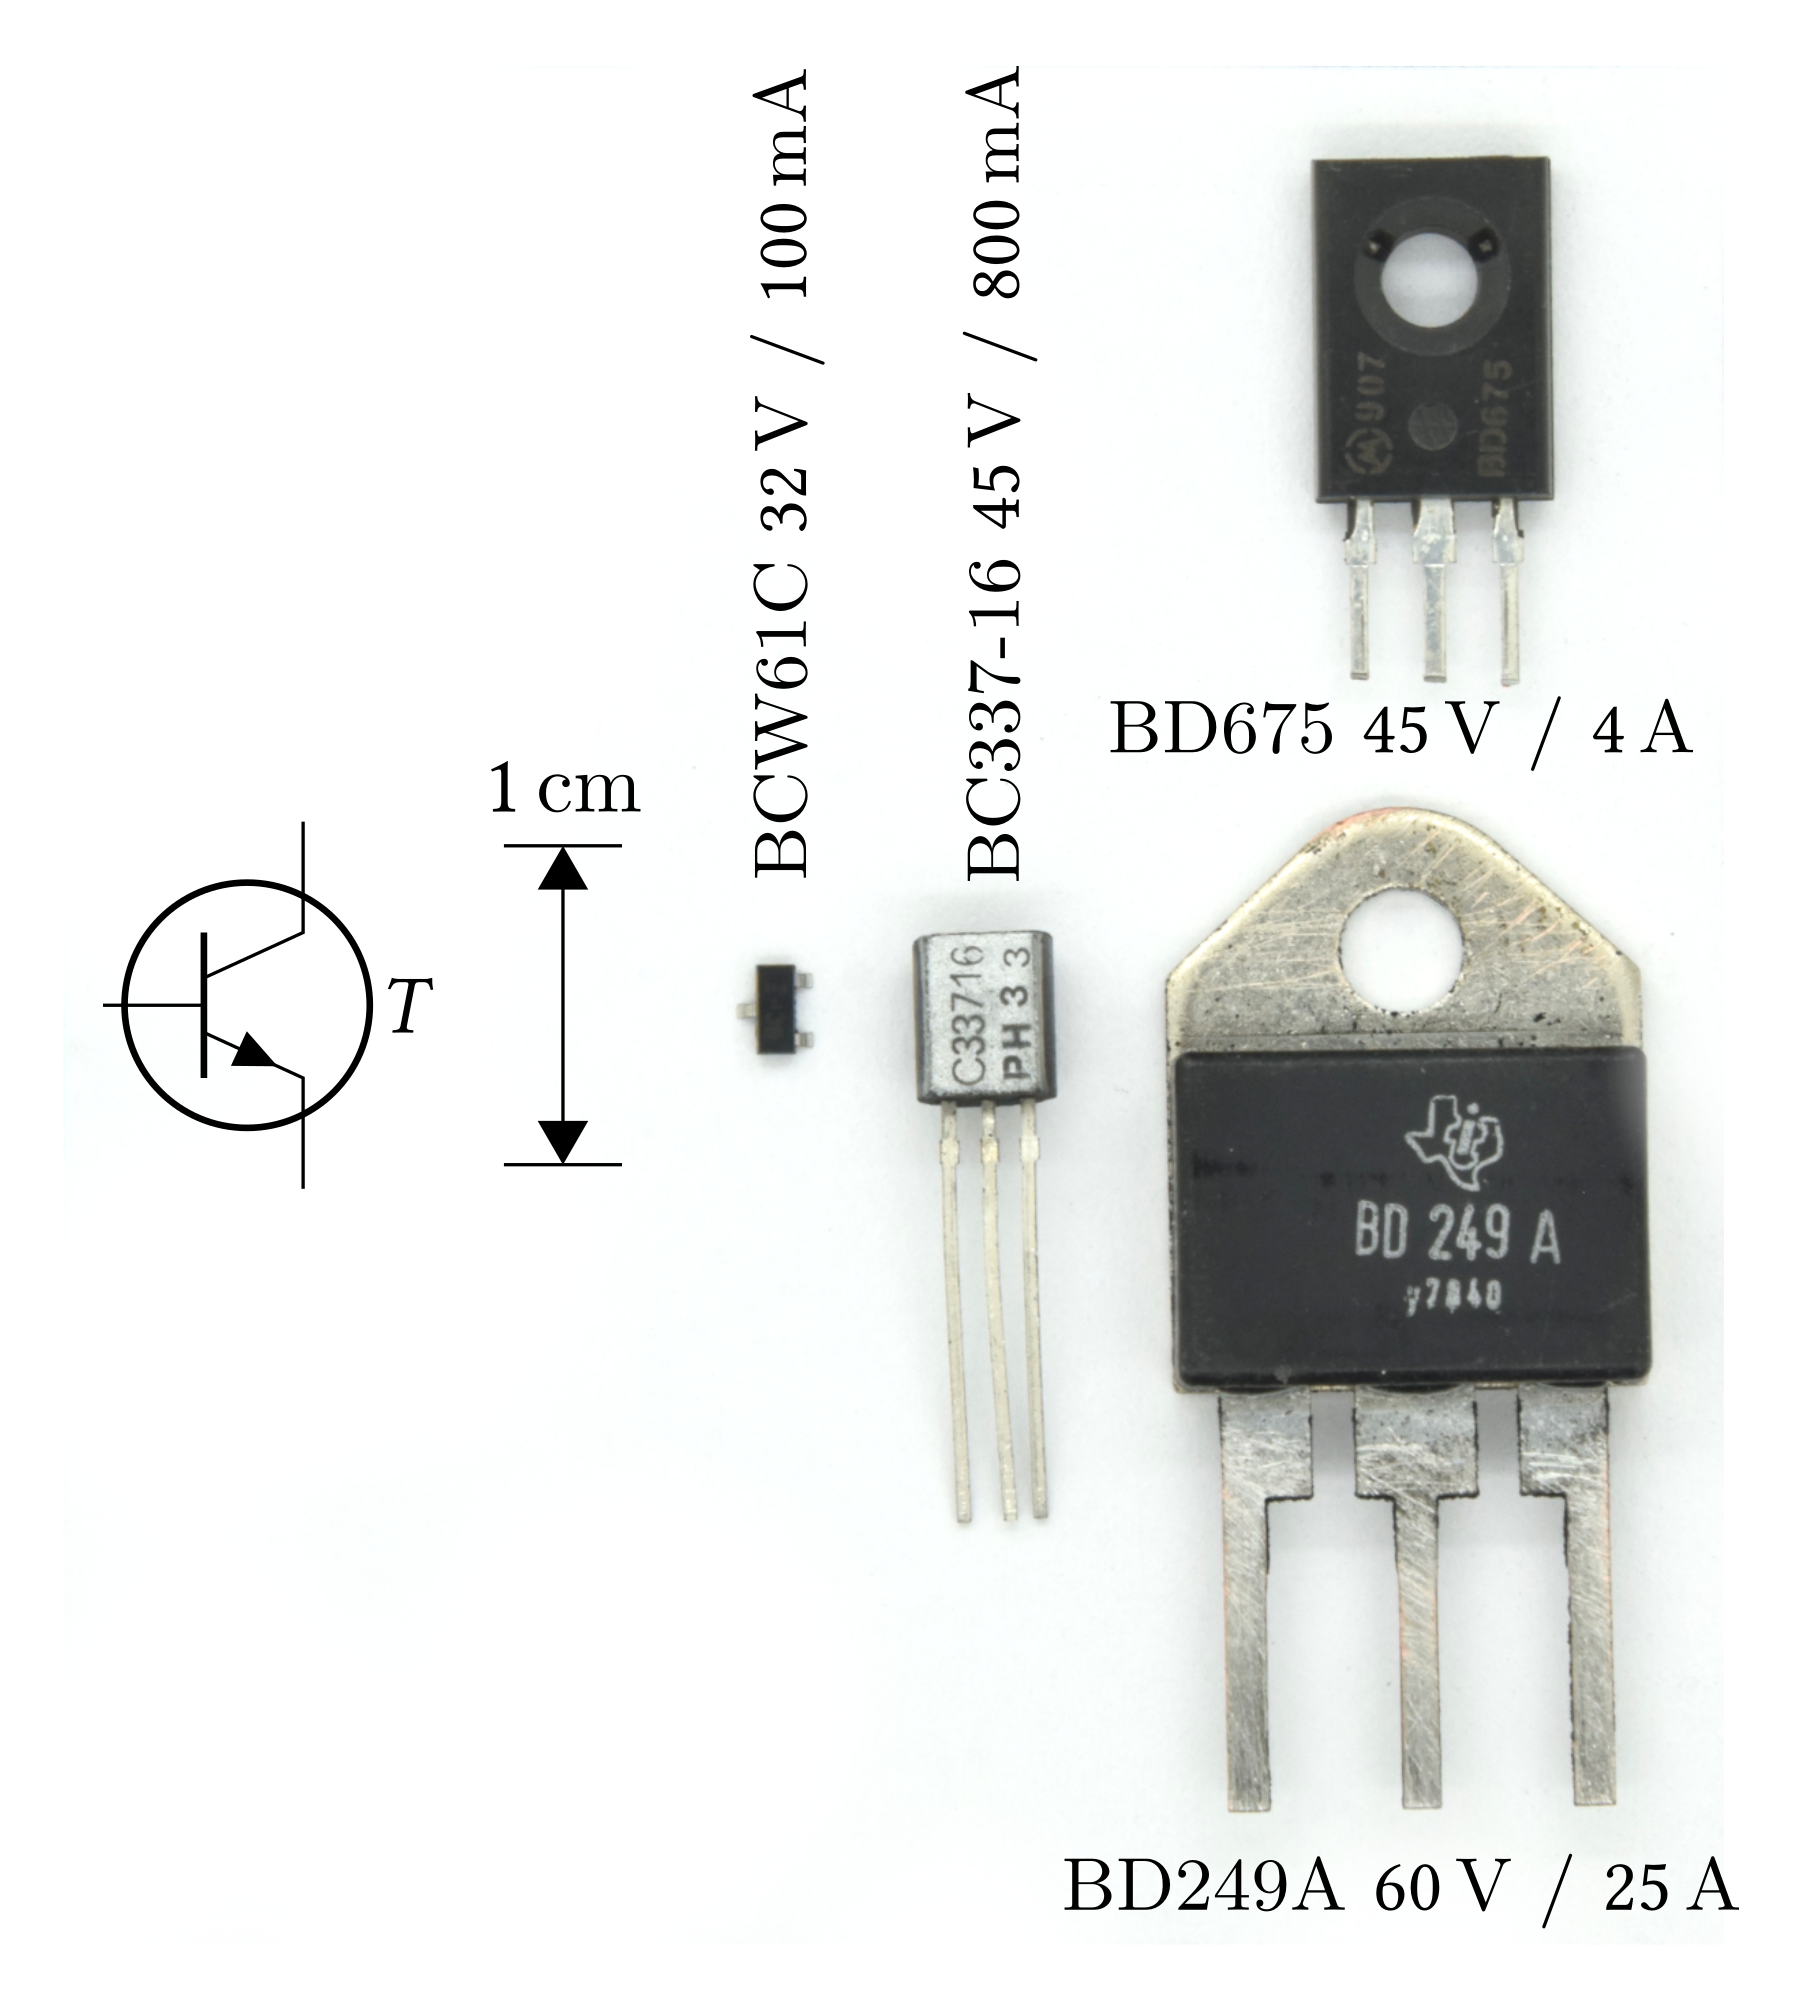
\includegraphics[width=0.85\textwidth]{foto/208}
    \caption{\scriptsize Schaltzeichen und Bauformen von Transistoren}
    \label{n_bauelemente_transistor}
\end{figure}

   \end{column}
\end{columns}

\end{frame}

\begin{frame}
\only<1>{
\begin{PQuestion}{NC501}{Welches Bauteil wird durch das Schaltzeichen symbolisiert?}{Diode}
{Spule}
{Kondensator}
{Transistor}
{\DARCimage{0.25\linewidth}{374include}}\end{PQuestion}

}
\only<2>{
\begin{PQuestion}{NC501}{Welches Bauteil wird durch das Schaltzeichen symbolisiert?}{Diode}
{Spule}
{Kondensator}
{\textbf{\textcolor{DARCgreen}{Transistor}}}
{\DARCimage{0.25\linewidth}{374include}}\end{PQuestion}

}
\end{frame}%ENDCONTENT


\title{DARC Amateurfunklehrgang Klasse NEA}
\author{Elektromagnetisches Feld}
\institute{Deutscher Amateur Radio Club e.\,V.}
\begin{frame}
\maketitle
\end{frame}

\section{Elektrisches Feld}
\label{section:e_feld}
\begin{frame}%STARTCONTENT

\frametitle{Homogenes elektrisches Feld}
\begin{columns}
    \begin{column}{0.48\textwidth}
    \begin{itemize}
  \item In einem Kondensator wird elektrische Energie gespeichert
  \item Die einfachste Art eines Kondensators ist der \emph{Plattenkondensator}
  \end{itemize}

    \end{column}
   \begin{column}{0.48\textwidth}
       
\begin{figure}
    \DARCimage{0.85\linewidth}{191include}
    \caption{\scriptsize Homogenes Feld in einem Plattenkondensator}
    \label{e_kondensator_homogenes_feld}
\end{figure}


   \end{column}
\end{columns}

\end{frame}

\begin{frame}
\begin{columns}
    \begin{column}{0.48\textwidth}
    \begin{itemize}
  \item An zwei elektrisch leitenden Platten wird jeweils der Plus- und Minus-Pol angeschlossen
  \item Zwischen den Platten baut sich ein homogenes elektrisches Feld (\emph{E-Feld}) auf
  \item Elektrische Feldstärke: $E = \dfrac{U}{d}$ in $\dfrac{V}{m}$
  \item Mit $d$ als Abstand der Platten
  \end{itemize}

    \end{column}
   \begin{column}{0.48\textwidth}
       
\begin{figure}
    \DARCimage{0.85\linewidth}{191include}
    \caption{\scriptsize Homogenes Feld in einem Plattenkondensator}
    \label{e_kondensator_homogenes_feld}
\end{figure}


   \end{column}
\end{columns}

\end{frame}

\begin{frame}
\only<1>{
\begin{PQuestion}{EB101}{Welches Feld stellt sich zwischen zwei parallelen Kondensatorplatten bei Anliegen einer Gleichspannung in Näherung ein?}{Polarisiertes elektrisches Feld}
{Homogenes magnetisches Feld}
{Homogenes elektrisches Feld}
{Polarisiertes magnetisches Feld}
{\DARCimage{1.0\linewidth}{191include}}\end{PQuestion}

}
\only<2>{
\begin{PQuestion}{EB101}{Welches Feld stellt sich zwischen zwei parallelen Kondensatorplatten bei Anliegen einer Gleichspannung in Näherung ein?}{Polarisiertes elektrisches Feld}
{Homogenes magnetisches Feld}
{\textbf{\textcolor{DARCgreen}{Homogenes elektrisches Feld}}}
{Polarisiertes magnetisches Feld}
{\DARCimage{1.0\linewidth}{191include}}\end{PQuestion}

}
\end{frame}

\begin{frame}
\only<1>{
\begin{QQuestion}{EA103}{Welche Einheit wird üblicherweise für die elektrische Feldstärke verwendet?}{Volt pro Meter (V/m)}
{Watt pro Meter (W/m)}
{Ampere pro Meter (A/m)}
{Henry pro Meter (H/m)}
\end{QQuestion}

}
\only<2>{
\begin{QQuestion}{EA103}{Welche Einheit wird üblicherweise für die elektrische Feldstärke verwendet?}{\textbf{\textcolor{DARCgreen}{Volt pro Meter (V/m)}}}
{Watt pro Meter (W/m)}
{Ampere pro Meter (A/m)}
{Henry pro Meter (H/m)}
\end{QQuestion}

}
\end{frame}

\begin{frame}
\only<1>{
\begin{QQuestion}{EB102}{An einem Plattenkondensator mit \qty{0,6}{\centi\metre} Plattenabstand werden \qty{9}{\volt} angelegt. Wie groß ist die elektrische Feldstärke zwischen den beiden Platten näherungsweise?}{\qty{5,4}{\V}/m}
{\qty{150}{\V}/m}
{\qty{540}{\V}/m}
{\qty{1500}{\V}/m}
\end{QQuestion}

}
\only<2>{
\begin{QQuestion}{EB102}{An einem Plattenkondensator mit \qty{0,6}{\centi\metre} Plattenabstand werden \qty{9}{\volt} angelegt. Wie groß ist die elektrische Feldstärke zwischen den beiden Platten näherungsweise?}{\qty{5,4}{\V}/m}
{\qty{150}{\V}/m}
{\qty{540}{\V}/m}
{\textbf{\textcolor{DARCgreen}{\qty{1500}{\V}/m}}}
\end{QQuestion}

}
\end{frame}

\begin{frame}
\frametitle{Wickelkondensator}
\begin{columns}
    \begin{column}{0.48\textwidth}
    \begin{itemize}
  \item Bei einem Wickelkondensator wird zwischen den beiden Platten als Metallbeläge ein Isolator als \emph{Dielektrikum} eingebracht
  \item Vorteile: platzsparend und größere Plattenfläche möglich
  \end{itemize}

    \end{column}
   \begin{column}{0.48\textwidth}
       
\begin{figure}
    \DARCimage{0.85\linewidth}{49include}
    \caption{\scriptsize Schematische Darstellung eines Wickelkondensators}
    \label{e_wickelkondensator}
\end{figure}


   \end{column}
\end{columns}

\end{frame}

\begin{frame}
\only<1>{
\begin{PQuestion}{EB103}{An den Metallbelägen eines Wickelkondensators mit \qty{0,15}{\mm} starkem Kunststoff-Dielektrikum liegt eine Spannung von \qty{300}{\V}. Wie hoch ist die elektrische Feldstärke zwischen den Metallbelägen ungefähr?}{\qty{2000}{\V}/m}
{\qty{200}{\V}/m}
{\qty{2000}{\kV}/m}
{\qty{200}{\kV}/m}
{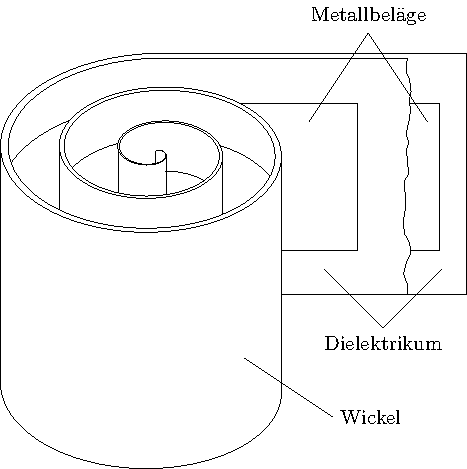
\includegraphics[width=1.0\linewidth]{img/49.pdf}}\end{PQuestion}

}
\only<2>{
\begin{PQuestion}{EB103}{An den Metallbelägen eines Wickelkondensators mit \qty{0,15}{\mm} starkem Kunststoff-Dielektrikum liegt eine Spannung von \qty{300}{\V}. Wie hoch ist die elektrische Feldstärke zwischen den Metallbelägen ungefähr?}{\qty{2000}{\V}/m}
{\qty{200}{\V}/m}
{\textbf{\textcolor{DARCgreen}{\qty{2000}{\kV}/m}}}
{\qty{200}{\kV}/m}
{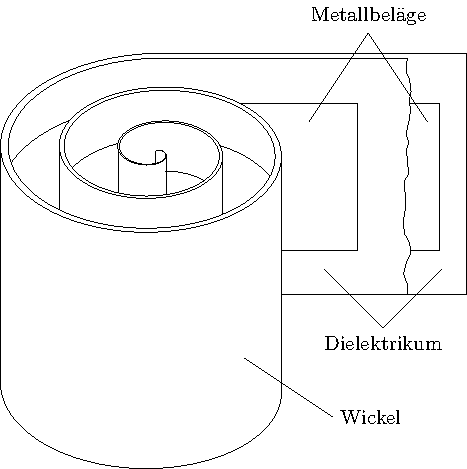
\includegraphics[width=1.0\linewidth]{img/49.pdf}}\end{PQuestion}

}
\end{frame}

\begin{frame}
\only<1>{
\begin{QQuestion}{EB104}{Ein Kondensator in einer Senderendstufe hat eine \qty{0,15}{\mm} starke PTFE-Folie als Dielektrikum. Die Durchschlagsfestigkeit von PTFE beträgt ca. \qty{400}{\kV}/cm. Wie groß wäre die maximale Spannung, die an den Kondensator angelegt werden kann, ohne dass die Folie durchschlagen wird?}{\qty{26}{\V}}
{\qty{60}{\kV}}
{\qty{6}{\kV}}
{\qty{2,6}{\kV}}
\end{QQuestion}

}
\only<2>{
\begin{QQuestion}{EB104}{Ein Kondensator in einer Senderendstufe hat eine \qty{0,15}{\mm} starke PTFE-Folie als Dielektrikum. Die Durchschlagsfestigkeit von PTFE beträgt ca. \qty{400}{\kV}/cm. Wie groß wäre die maximale Spannung, die an den Kondensator angelegt werden kann, ohne dass die Folie durchschlagen wird?}{\qty{26}{\V}}
{\qty{60}{\kV}}
{\textbf{\textcolor{DARCgreen}{\qty{6}{\kV}}}}
{\qty{2,6}{\kV}}
\end{QQuestion}

}
\end{frame}

\begin{frame}
\frametitle{Lösungsweg}
Der Trick ist hier, dass die Durschlagsfestigkeit die elektrische Feldstärke $E$ ist.

\begin{itemize}
  \item Gegeben: $d = 0,15mm$ und $E = 400\frac{kV}{cm}$
  \item Gesucht: $U$
  \item Lösung:
  \end{itemize}
$E = \frac{U}{d} \Rightarrow U = E\cdot d$

$U = 400\cdot\frac{10^3V}{10^{-2}m}\cdot 0,15\cdot 10^{-3}m$

$U = 6\cdot10^3V = 6kV$

\end{frame}

\begin{frame}
\frametitle{Vertikalantenne}
\begin{columns}
    \begin{column}{0.48\textwidth}
    \begin{itemize}
  \item An einer Antenne entstehen ebenso elektrische Feldlinien
  \item Die Feldlinien einer Vertikalantenne verlaufen vom \enquote{positiven Ende} zur Erde
  \end{itemize}

    \end{column}
   \begin{column}{0.48\textwidth}
       
\begin{figure}
    \DARCimage{0.85\linewidth}{193include}
    \caption{\scriptsize Feldlinien an einer Vertikalantenne}
    \label{e_feldlinien_vertikalantenne}
\end{figure}


   \end{column}
\end{columns}

\end{frame}

\begin{frame}
\only<1>{
\begin{PQuestion}{EB105}{Wie werden die mit X gekennzeichneten Feldlinien einer Vertikalantenne bezeichnet?}{Radiale Feldlinien}
{Magnetische Feldlinien}
{Elektrische Feldlinien}
{Horizontale Feldlinien}
{\DARCimage{1.0\linewidth}{193include}}\end{PQuestion}

}
\only<2>{
\begin{PQuestion}{EB105}{Wie werden die mit X gekennzeichneten Feldlinien einer Vertikalantenne bezeichnet?}{Radiale Feldlinien}
{Magnetische Feldlinien}
{\textbf{\textcolor{DARCgreen}{Elektrische Feldlinien}}}
{Horizontale Feldlinien}
{\DARCimage{1.0\linewidth}{193include}}\end{PQuestion}

}
\end{frame}%ENDCONTENT


\section{Magnetisches Feld}
\label{section:h_feld}
\begin{frame}%STARTCONTENT

\frametitle{Stromdurchflossener Leiter}
\begin{columns}
    \begin{column}{0.48\textwidth}
    \begin{itemize}
  \item Fließt Strom durch einen Leiter, bilden sich konzentrische, magnetische Felder um den Leiter
  \end{itemize}

    \end{column}
   \begin{column}{0.48\textwidth}
       Grafik eines stromdurchflossenen Leiters mit konzentrischen magnetischen Feldlinien kommt noch


   \end{column}
\end{columns}

\end{frame}

\begin{frame}
\only<1>{
\begin{QQuestion}{EB201}{Wenn ein konstanter Gleichstrom durch einen gestreckten Leiter fließt, sind die~...}{magnetischen Feldlinien sternförmig um den Leiter.}
{elektrischen Feldlinien konzentrische Kreise um den Leiter.}
{magnetischen Feldlinien konzentrische Kreise um den Leiter.}
{elektrischen Feldlinien parallel zu den magnetischen Feldlinien um den Leiter.}
\end{QQuestion}

}
\only<2>{
\begin{QQuestion}{EB201}{Wenn ein konstanter Gleichstrom durch einen gestreckten Leiter fließt, sind die~...}{magnetischen Feldlinien sternförmig um den Leiter.}
{elektrischen Feldlinien konzentrische Kreise um den Leiter.}
{\textbf{\textcolor{DARCgreen}{magnetischen Feldlinien konzentrische Kreise um den Leiter.}}}
{elektrischen Feldlinien parallel zu den magnetischen Feldlinien um den Leiter.}
\end{QQuestion}

}
\end{frame}

\begin{frame}
\frametitle{Homogenes magnetisches Feld}
\begin{columns}
    \begin{column}{0.48\textwidth}
    \begin{itemize}
  \item Wird ein stromdurchflossener Leiter zu einer Zylinderspule aufgewickelt, entsteht im inneren ein homogenes magnetisches Feld (\emph{H-Feld})
  \item Eine Spule speichert magnetische Energie
  \end{itemize}

    \end{column}
   \begin{column}{0.48\textwidth}
       
\begin{figure}
    \DARCimage{0.85\linewidth}{50include}
    \caption{\scriptsize Magnetische Feldlinien in einer Zylinderspule}
    \label{e_h_feld_spule}
\end{figure}

\begin{itemize}
  \item Einheit: $\dfrac{A}{m}$
  \end{itemize}

   \end{column}
\end{columns}

\end{frame}

\begin{frame}
\only<1>{
\begin{PQuestion}{EB202}{Welches Feld stellt sich im Inneren einer langen Zylinderspule bei Fließen eines Gleichstroms näherungsweise ein?}{Homogenes magnetisches Feld}
{Homogenes elektrisches Feld}
{Konzentrisches magnetisches Feld}
{Zentriertes magnetisches Feld}
{\DARCimage{1.0\linewidth}{50include}}\end{PQuestion}

}
\only<2>{
\begin{PQuestion}{EB202}{Welches Feld stellt sich im Inneren einer langen Zylinderspule bei Fließen eines Gleichstroms näherungsweise ein?}{\textbf{\textcolor{DARCgreen}{Homogenes magnetisches Feld}}}
{Homogenes elektrisches Feld}
{Konzentrisches magnetisches Feld}
{Zentriertes magnetisches Feld}
{\DARCimage{1.0\linewidth}{50include}}\end{PQuestion}

}
\end{frame}

\begin{frame}
\only<1>{
\begin{QQuestion}{EA104}{Welche Einheit wird üblicherweise für die magnetische Feldstärke verwendet?}{Ampere pro Meter (A/m)}
{Watt pro Meter (W/m)}
{Volt pro Meter (V/m)}
{Henry pro Meter (H/m)}
\end{QQuestion}

}
\only<2>{
\begin{QQuestion}{EA104}{Welche Einheit wird üblicherweise für die magnetische Feldstärke verwendet?}{\textbf{\textcolor{DARCgreen}{Ampere pro Meter (A/m)}}}
{Watt pro Meter (W/m)}
{Volt pro Meter (V/m)}
{Henry pro Meter (H/m)}
\end{QQuestion}

}
\end{frame}

\begin{frame}
\frametitle{Ringkern}
\begin{columns}
    \begin{column}{0.48\textwidth}
    \begin{itemize}
  \item Leiter wird auf einen magnetisch leitenden Ringkern gewickelt, z.B. Eisen
  \item Vorteile: Platzsparend und stabiler
  \end{itemize}

    \end{column}
   \begin{column}{0.48\textwidth}
       
\begin{figure}
    \DARCimage{0.85\linewidth}{40include}
    \caption{\scriptsize Ringkernspule}
    \label{e_ringkern}
\end{figure}


   \end{column}
\end{columns}

\end{frame}

\begin{frame}
\begin{columns}
    \begin{column}{0.48\textwidth}
    \begin{itemize}
  \item Magnetische Feldstärke $H = \dfrac{I\cdot N}{l_m}$ in $\dfrac{A}{m}$
  \item mit $N$ als Wicklungsanzahl und $l_m$ mittlere Länge des Rings
  \end{itemize}

    \end{column}
   \begin{column}{0.48\textwidth}
       
\begin{figure}
    \DARCimage{0.85\linewidth}{40include}
    \caption{\scriptsize Ringkernspule}
    \label{e_ringkern}
\end{figure}


   \end{column}
\end{columns}

\end{frame}

\begin{frame}
\only<1>{
\begin{PQuestion}{EB203}{Ein Ringkern hat einen mittleren Durchmesser von \qty{2,6}{\cm} und trägt 6 Windungen Kupferdraht. Wie groß ist die mittlere magnetische Feldstärke im Ringkern, wenn der Strom \qty{2,5}{\A} beträgt?}{\qty{183,6}{\A}/m}
{\qty{1,836}{\A}/m}
{\qty{5769}{\A}/m}
{\qty{5,769}{\A}/m}
{\DARCimage{0.5\linewidth}{40include}}\end{PQuestion}

}
\only<2>{
\begin{PQuestion}{EB203}{Ein Ringkern hat einen mittleren Durchmesser von \qty{2,6}{\cm} und trägt 6 Windungen Kupferdraht. Wie groß ist die mittlere magnetische Feldstärke im Ringkern, wenn der Strom \qty{2,5}{\A} beträgt?}{\textbf{\textcolor{DARCgreen}{\qty{183,6}{\A}/m}}}
{\qty{1,836}{\A}/m}
{\qty{5769}{\A}/m}
{\qty{5,769}{\A}/m}
{\DARCimage{0.5\linewidth}{40include}}\end{PQuestion}

}

\end{frame}

\begin{frame}
\only<1>{
\begin{QQuestion}{EB204}{Welcher der nachfolgenden Werkstoffe ist bei Raumtemperatur ein ferromagnetischer Stoff?}{Kupfer}
{Chrom}
{Eisen}
{Aluminium}
\end{QQuestion}

}
\only<2>{
\begin{QQuestion}{EB204}{Welcher der nachfolgenden Werkstoffe ist bei Raumtemperatur ein ferromagnetischer Stoff?}{Kupfer}
{Chrom}
{\textbf{\textcolor{DARCgreen}{Eisen}}}
{Aluminium}
\end{QQuestion}

}
\end{frame}

\begin{frame}
\frametitle{Magnetfeld einer Antenne}
\begin{columns}
    \begin{column}{0.48\textwidth}
    \begin{itemize}
  \item An einer Antenne wirkt das Magnetfeld um den Leiter
  \item Hier an einer Vertikalantenne konzentrisch um die Antenne
  \end{itemize}

    \end{column}
   \begin{column}{0.48\textwidth}
       
\begin{figure}
    \DARCimage{0.85\linewidth}{192include}
    \caption{\scriptsize Magnetfeld an einer Vertikalantenne}
    \label{e_vertikalantenne_magnetfeld}
\end{figure}


   \end{column}
\end{columns}

\end{frame}

\begin{frame}
\only<1>{
\begin{PQuestion}{EB206}{Wie werden die mit X gekennzeichneten Feldlinien einer Vertikalantenne bezeichnet?}{Offene Feldlinien}
{Elektrische Feldlinien}
{Magnetische Feldlinien}
{Vertikale Feldlinien}
{\DARCimage{1.0\linewidth}{192include}}\end{PQuestion}

}
\only<2>{
\begin{PQuestion}{EB206}{Wie werden die mit X gekennzeichneten Feldlinien einer Vertikalantenne bezeichnet?}{Offene Feldlinien}
{Elektrische Feldlinien}
{\textbf{\textcolor{DARCgreen}{Magnetische Feldlinien}}}
{Vertikale Feldlinien}
{\DARCimage{1.0\linewidth}{192include}}\end{PQuestion}

}
\end{frame}%ENDCONTENT


\section{Elektromagnetisches Feld}
\label{section:em_feld}
\begin{frame}%STARTCONTENT

\begin{columns}
    \begin{column}{0.48\textwidth}
    \begin{itemize}
  \item Fließt ein zeitlich veränderlicher Strom durch einen Leiter, z.B. eine Antenne, entsteht sowohl ein elektrisches als auch ein magnetisches Feld
  \item Dieses wird als elektromagnetisches Feld bezeichnet
  \item Die beiden Felder stehen in einem 90º-Winkel zueinander
  \end{itemize}

    \end{column}
   \begin{column}{0.48\textwidth}
       
\begin{figure}
    \DARCimage{0.85\linewidth}{192include}
    \caption{\scriptsize Elektrisches und magnetisches Feld an einer Antenne}
    \label{e_vertikalantenne_magnetfeld}
\end{figure}


   \end{column}
\end{columns}

\end{frame}

\begin{frame}
\only<1>{
\begin{QQuestion}{EB301}{Wodurch entsteht ein elektromagnetisches Feld beispielsweise?}{Ein elektromagnetisches Feld entsteht, wenn ein zeitlich konstanter Strom durch einen elektrischen Leiter fließt.}
{Ein elektromagnetisches Feld entsteht, wenn ein zeitlich veränderlicher Strom durch einen elektrischen Leiter fließt.}
{Ein elektromagnetisches Feld entsteht, wenn eine zeitlich konstante Spannung an einem elektrischen Leiter anliegt.}
{Ein elektromagnetisches Feld entsteht, wenn eine zeitlich konstante Spannung an einem elektrischen Isolator anliegt.}
\end{QQuestion}

}
\only<2>{
\begin{QQuestion}{EB301}{Wodurch entsteht ein elektromagnetisches Feld beispielsweise?}{Ein elektromagnetisches Feld entsteht, wenn ein zeitlich konstanter Strom durch einen elektrischen Leiter fließt.}
{\textbf{\textcolor{DARCgreen}{Ein elektromagnetisches Feld entsteht, wenn ein zeitlich veränderlicher Strom durch einen elektrischen Leiter fließt.}}}
{Ein elektromagnetisches Feld entsteht, wenn eine zeitlich konstante Spannung an einem elektrischen Leiter anliegt.}
{Ein elektromagnetisches Feld entsteht, wenn eine zeitlich konstante Spannung an einem elektrischen Isolator anliegt.}
\end{QQuestion}

}
\end{frame}

\begin{frame}
\only<1>{
\begin{QQuestion}{EB302}{Wie erfolgt die Ausbreitung einer elektromagnetischen Welle? Die Ausbreitung erfolgt~...}{nur über das magnetische Feld. Das elektrische Feld wirkt sich nur im Nahfeld aus.}
{nur über das elektrische Feld. Das magnetische Feld wirkt sich nur im Nahfeld aus.}
{durch eine Wechselwirkung zwischen elektrischem und magnetischem Feld.}
{durch die unabhängige Ausbreitung von elektrischem und magnetischem Feld.}
\end{QQuestion}

}
\only<2>{
\begin{QQuestion}{EB302}{Wie erfolgt die Ausbreitung einer elektromagnetischen Welle? Die Ausbreitung erfolgt~...}{nur über das magnetische Feld. Das elektrische Feld wirkt sich nur im Nahfeld aus.}
{nur über das elektrische Feld. Das magnetische Feld wirkt sich nur im Nahfeld aus.}
{\textbf{\textcolor{DARCgreen}{durch eine Wechselwirkung zwischen elektrischem und magnetischem Feld.}}}
{durch die unabhängige Ausbreitung von elektrischem und magnetischem Feld.}
\end{QQuestion}

}
\end{frame}

\begin{frame}
\only<1>{
\begin{QQuestion}{EB303}{Der Winkel zwischen den elektrischen und magnetischen Feldkomponenten eines elektromagnetischen Feldes beträgt bei Freiraumausbreitung im Fernfeld~...}{\qty{90}{\degree}.}
{\qty{45}{\degree}.}
{\qty{180}{\degree}.}
{\qty{360}{\degree}.}
\end{QQuestion}

}
\only<2>{
\begin{QQuestion}{EB303}{Der Winkel zwischen den elektrischen und magnetischen Feldkomponenten eines elektromagnetischen Feldes beträgt bei Freiraumausbreitung im Fernfeld~...}{\textbf{\textcolor{DARCgreen}{\qty{90}{\degree}.}}}
{\qty{45}{\degree}.}
{\qty{180}{\degree}.}
{\qty{360}{\degree}.}
\end{QQuestion}

}
\end{frame}

\begin{frame}
\only<1>{
\begin{QQuestion}{EB304}{Welche Aussage trifft auf die elektromagnetische Ausstrahlung im ungestörten Fernfeld zu?}{Die E-Feldkomponente und die H-Feldkomponente sind phasengleich und sind parallel zueinander. Die Ausbreitungsrichtung verläuft dazu in einem rechten Winkel.}
{Die E-Feldkomponente und die H-Feldkomponente stehen in einem rechten Winkel zueinander. Die Ausbreitungsrichtung hat keine feste Beziehung dazu.}
{Die E-Feldkomponente, die H-Feldkomponente und die Ausbreitungsrichtung stehen in einem rechten Winkel zueinander.}
{Die Ausbreitungsrichtung befindet sich parallel zur E-Feldkomponente und verläuft senkrecht zur H-Feldkomponente.}
\end{QQuestion}

}
\only<2>{
\begin{QQuestion}{EB304}{Welche Aussage trifft auf die elektromagnetische Ausstrahlung im ungestörten Fernfeld zu?}{Die E-Feldkomponente und die H-Feldkomponente sind phasengleich und sind parallel zueinander. Die Ausbreitungsrichtung verläuft dazu in einem rechten Winkel.}
{Die E-Feldkomponente und die H-Feldkomponente stehen in einem rechten Winkel zueinander. Die Ausbreitungsrichtung hat keine feste Beziehung dazu.}
{\textbf{\textcolor{DARCgreen}{Die E-Feldkomponente, die H-Feldkomponente und die Ausbreitungsrichtung stehen in einem rechten Winkel zueinander.}}}
{Die Ausbreitungsrichtung befindet sich parallel zur E-Feldkomponente und verläuft senkrecht zur H-Feldkomponente.}
\end{QQuestion}

}
\end{frame}%ENDCONTENT


\section{Polarisation elektromagnetischer Wellen}
\label{section:em_feld_polarisation}
\begin{frame}%STARTCONTENT

\frametitle{Horizontale Polarisation}
\begin{columns}
    \begin{column}{0.48\textwidth}
    \begin{itemize}
  \item Die Lage des E-Feldes gibt die Polarisation an
  \item Breitet sich das E-Feld horizontal aus, wird von horizontaler Polarisation gesprochen
  \item Ist von Bauform der Antenne abhängig
  \end{itemize}

    \end{column}
   \begin{column}{0.48\textwidth}
       
\begin{figure}
    \DARCimage{0.85\linewidth}{194include}
    \caption{\scriptsize Horizontale Polarisation in einem Feld}
    \label{e_horizontale_polarisation}
\end{figure}


   \end{column}
\end{columns}

\end{frame}

\begin{frame}
\only<1>{
\begin{QQuestion}{EB305}{Die Polarisation einer elektromagnetischen Welle ist durch die Richtung~...}{der Ausbreitung (S-Vektor/Poynting-Vektor) bestimmt.}
{des magnetischen Nordpols (relativ zur Antenne) bestimmt.}
{des elektrischen Feldes (Vektor des E-Feldes) bestimmt.}
{des unmittelbaren Nahfeldes ($\lambda/4$-Bereich) bestimmt.}
\end{QQuestion}

}
\only<2>{
\begin{QQuestion}{EB305}{Die Polarisation einer elektromagnetischen Welle ist durch die Richtung~...}{der Ausbreitung (S-Vektor/Poynting-Vektor) bestimmt.}
{des magnetischen Nordpols (relativ zur Antenne) bestimmt.}
{\textbf{\textcolor{DARCgreen}{des elektrischen Feldes (Vektor des E-Feldes) bestimmt.}}}
{des unmittelbaren Nahfeldes ($\lambda/4$-Bereich) bestimmt.}
\end{QQuestion}

}
\end{frame}

\begin{frame}
\only<1>{
\begin{PQuestion}{EB306}{Das folgende Bild zeigt eine Momentaufnahme eines elektromagnetischen Feldes. Welche Polarisation hat die skizzierte Welle?}{Rechtszirkulare Polarisation}
{Vertikale Polarisation}
{Horizontale Polarisation}
{Linkszirkulare Polarisation}
{\DARCimage{1.0\linewidth}{194include}}\end{PQuestion}

}
\only<2>{
\begin{PQuestion}{EB306}{Das folgende Bild zeigt eine Momentaufnahme eines elektromagnetischen Feldes. Welche Polarisation hat die skizzierte Welle?}{Rechtszirkulare Polarisation}
{Vertikale Polarisation}
{\textbf{\textcolor{DARCgreen}{Horizontale Polarisation}}}
{Linkszirkulare Polarisation}
{\DARCimage{1.0\linewidth}{194include}}\end{PQuestion}

}
\end{frame}

\begin{frame}
\only<1>{
\begin{PQuestion}{EB309}{Die Polarisation des Sendesignals in der Hauptstrahlrichtung dieser Richtantenne ist~...}{linksdrehend.}
{vertikal.}
{rechtsdrehend.}
{horizontal.}
{\DARCimage{1.0\linewidth}{326include}}\end{PQuestion}

}
\only<2>{
\begin{PQuestion}{EB309}{Die Polarisation des Sendesignals in der Hauptstrahlrichtung dieser Richtantenne ist~...}{linksdrehend.}
{vertikal.}
{rechtsdrehend.}
{\textbf{\textcolor{DARCgreen}{horizontal.}}}
{\DARCimage{1.0\linewidth}{326include}}\end{PQuestion}

}
\end{frame}

\begin{frame}
\frametitle{Vertikale Polarisation}
\begin{columns}
    \begin{column}{0.48\textwidth}
    \begin{itemize}
  \item Die Lage des E-Feldes gibt die Polarisation an
  \item Breitet sich das E-Feld vertikal aus, wird von vertikaler Polarisation gesprochen
  \item Ist von Bauform der Antenne abhängig
  \end{itemize}

    \end{column}
   \begin{column}{0.48\textwidth}
       
\begin{figure}
    \DARCimage{0.85\linewidth}{203include}
    \caption{\scriptsize Vertikale Polarisation in einem Feld}
    \label{e_vertikale_polarisation}
\end{figure}


   \end{column}
\end{columns}

\end{frame}

\begin{frame}
\only<1>{
\begin{PQuestion}{EB307}{Das folgende Bild zeigt eine Momentaufnahme eines elektromagnetischen Feldes. Welche Polarisation hat die skizzierte Welle?}{Vertikale Polarisation}
{Horizontale Polarisation}
{Linkszirkulare Polarisation}
{Rechtszirkulare Polarisation}
{\DARCimage{1.0\linewidth}{203include}}\end{PQuestion}

}
\only<2>{
\begin{PQuestion}{EB307}{Das folgende Bild zeigt eine Momentaufnahme eines elektromagnetischen Feldes. Welche Polarisation hat die skizzierte Welle?}{\textbf{\textcolor{DARCgreen}{Vertikale Polarisation}}}
{Horizontale Polarisation}
{Linkszirkulare Polarisation}
{Rechtszirkulare Polarisation}
{\DARCimage{1.0\linewidth}{203include}}\end{PQuestion}

}
\end{frame}

\begin{frame}
\only<1>{
\begin{PQuestion}{EB310}{Die Polarisation des Sendesignals in der Hauptstrahlrichtung dieser Richtantenne ist~...}{horizontal.}
{vertikal.}
{rechtsdrehend.}
{linksdrehend.}
{\DARCimage{1.0\linewidth}{51include}}\end{PQuestion}

}
\only<2>{
\begin{PQuestion}{EB310}{Die Polarisation des Sendesignals in der Hauptstrahlrichtung dieser Richtantenne ist~...}{horizontal.}
{\textbf{\textcolor{DARCgreen}{vertikal.}}}
{rechtsdrehend.}
{linksdrehend.}
{\DARCimage{1.0\linewidth}{51include}}\end{PQuestion}

}
\end{frame}

\begin{frame}
\frametitle{Zirkulare Polarisation}
\begin{columns}
    \begin{column}{0.48\textwidth}
    \begin{itemize}
  \item Die Lage des E-Feldes gibt die Polarisation an
  \item Breitet sich das E-Feld zirkular aus, wird von zirkularer Polarisation gesprochen
  \item Es ist rechts- und linksdrehend möglich
  \item Ist von Bauform der Antenne abhängig
  \end{itemize}

    \end{column}
   \begin{column}{0.48\textwidth}
       
\begin{figure}
    \DARCimage{0.85\linewidth}{204include}
    \caption{\scriptsize Zirkulare Polarisation in einem Feld}
    \label{e_zirkulare_polarisation}
\end{figure}


   \end{column}
\end{columns}

\end{frame}

\begin{frame}
\only<1>{
\begin{PQuestion}{EB308}{Das folgende Bild zeigt eine Momentaufnahme eines elektromagnetischen Feldes. Welche Polarisation hat die skizzierte Welle?}{Zirkulare Polarisation}
{Horizontale Polarisation}
{Vertikale Polarisation}
{Diagonale Polarisation}
{\DARCimage{1.0\linewidth}{204include}}\end{PQuestion}

}
\only<2>{
\begin{PQuestion}{EB308}{Das folgende Bild zeigt eine Momentaufnahme eines elektromagnetischen Feldes. Welche Polarisation hat die skizzierte Welle?}{\textbf{\textcolor{DARCgreen}{Zirkulare Polarisation}}}
{Horizontale Polarisation}
{Vertikale Polarisation}
{Diagonale Polarisation}
{\DARCimage{1.0\linewidth}{204include}}\end{PQuestion}

}
\end{frame}%ENDCONTENT


\title{DARC Amateurfunklehrgang Klasse NEA}
\author{Bauelemente}
\institute{Deutscher Amateur Radio Club e.\,V.}
\begin{frame}
\maketitle
\end{frame}

\section{Kondensator I}
\label{section:kondensator_1}
\begin{frame}%STARTCONTENT

\frametitle{Kapazität}
\begin{itemize}
  \item Wichtigste Eigenschaft des Kondensators: Ladung speichern
  \item $\rightarrow$ Kapazität
  \end{itemize}
$C = \dfrac{Q}{U}$

\begin{itemize}
  \item mit $Q$ als elektrische Ladung
  \item Einheit: $\frac{As}{V}$ bzw. Farad $F$
  \item Die Kapazität ist die elektrische Ladung pro Volt
  \end{itemize}

\end{frame}

\begin{frame}
\frametitle{Kapazität durch Bauart}
\begin{columns}
    \begin{column}{0.48\textwidth}
    \begin{itemize}
  \item Die Kapazität kann durch die Bauart erreicht werden
  \end{itemize}
$C = \dfrac{\varepsilon_0 \cdot \varepsilon_r \cdot A}{d}$

\begin{itemize}
  \item $\rightarrow$ Kapazität ist größer bei größerer Fläche, kleinem Abstand oder anderem Dielektrikum
  \end{itemize}

    \end{column}
   \begin{column}{0.48\textwidth}
       \begin{itemize}
  \item $\varepsilon_0 = 0,855 \cdot 10^{-11}\frac{As}{Vm}$: elektrische Feldkonstante
  \item $\varepsilon_r$: relative Dielektrizitätszahl, abhängig vom Dielektrikum (ohne Einheit)
  \item $A$: Fläche der Kondensatorplatten
  \item $d$: Abstand der Platten
  \end{itemize}

   \end{column}
\end{columns}

\end{frame}

\begin{frame}
\only<1>{
\begin{QQuestion}{EA101}{Welche Einheit wird üblicherweise für die Kapazität verwendet?}{Amperestunden (Ah)}
{Ohm ($\Omega$)}
{Farad (F)}
{Henry (H)}
\end{QQuestion}

}
\only<2>{
\begin{QQuestion}{EA101}{Welche Einheit wird üblicherweise für die Kapazität verwendet?}{Amperestunden (Ah)}
{Ohm ($\Omega$)}
{\textbf{\textcolor{DARCgreen}{Farad (F)}}}
{Henry (H)}
\end{QQuestion}

}
\end{frame}

\begin{frame}
\only<1>{
\begin{QQuestion}{EC205}{Von welcher der nachfolgenden Größen ist die Kapazität eines Plattenkondensators \underline{nicht} abhängig?}{Plattenabstand}
{Spannung}
{Plattenfläche}
{Dielektrikum}
\end{QQuestion}

}
\only<2>{
\begin{QQuestion}{EC205}{Von welcher der nachfolgenden Größen ist die Kapazität eines Plattenkondensators \underline{nicht} abhängig?}{Plattenabstand}
{\textbf{\textcolor{DARCgreen}{Spannung}}}
{Plattenfläche}
{Dielektrikum}
\end{QQuestion}

}
\end{frame}

\begin{frame}
\only<1>{
\begin{QQuestion}{EC203}{Wodurch verringert sich die Kapazität eines Plattenkondensators? Durch~...}{eine größere Dielektrizitätskonstante des Dielektrikums.}
{einen größeren Plattenabstand.}
{eine größere Spannung.}
{größere Plattenflächen.}
\end{QQuestion}

}
\only<2>{
\begin{QQuestion}{EC203}{Wodurch verringert sich die Kapazität eines Plattenkondensators? Durch~...}{eine größere Dielektrizitätskonstante des Dielektrikums.}
{\textbf{\textcolor{DARCgreen}{einen größeren Plattenabstand.}}}
{eine größere Spannung.}
{größere Plattenflächen.}
\end{QQuestion}

}
\end{frame}

\begin{frame}
\only<1>{
\begin{QQuestion}{EC204}{In welchem Fall sinkt die Kapazität eines Plattenkondensators?}{Bei Vergrößerung der Plattenoberfläche}
{Bei Erhöhung der angelegten Spannung}
{Bei Vergrößerung des Plattenabstandes}
{Bei Vergrößerung der Dielektrizitätszahl}
\end{QQuestion}

}
\only<2>{
\begin{QQuestion}{EC204}{In welchem Fall sinkt die Kapazität eines Plattenkondensators?}{Bei Vergrößerung der Plattenoberfläche}
{Bei Erhöhung der angelegten Spannung}
{\textbf{\textcolor{DARCgreen}{Bei Vergrößerung des Plattenabstandes}}}
{Bei Vergrößerung der Dielektrizitätszahl}
\end{QQuestion}

}
\end{frame}

\begin{frame}
\frametitle{Drehkondensator}
\begin{columns}
    \begin{column}{0.48\textwidth}
    \begin{itemize}
  \item Eine Platte ist feststehend, die andere Platte kann rotiert werden
  \item Nur dort, wo die Platten sich überlappen, wirkt der Kondensator
  \item Die Fläche wird durch Drehung verändert $\rightarrow$ Änderung der Kapazität
  \end{itemize}

    \end{column}
   \begin{column}{0.48\textwidth}
       
\begin{figure}
    \DARCimage{0.85\linewidth}{840include}
    \caption{\scriptsize Drehkondensator}
    \label{e_kondensator_drehkondensator}
\end{figure}


   \end{column}
\end{columns}

\end{frame}

\begin{frame}
\only<1>{
\begin{QQuestion}{EC206}{Wie nennt man ein Bauelement, bei dem sich Platten auf einer isolierten Achse befinden, die zwischen fest stehenden Platten rotiert werden können?}{Drehkondensator}
{Styroflexkondensator}
{Keramischer Kondensator}
{Rotorkondensator}
\end{QQuestion}

}
\only<2>{
\begin{QQuestion}{EC206}{Wie nennt man ein Bauelement, bei dem sich Platten auf einer isolierten Achse befinden, die zwischen fest stehenden Platten rotiert werden können?}{\textbf{\textcolor{DARCgreen}{Drehkondensator}}}
{Styroflexkondensator}
{Keramischer Kondensator}
{Rotorkondensator}
\end{QQuestion}

}
\end{frame}

\begin{frame}
\frametitle{Elektrolytkondensator}
\begin{columns}
    \begin{column}{0.48\textwidth}
    \begin{itemize}
  \item Spezielle Bauform
  \item Ermöglicht große Kapazität
  \item Nur für Gleichspannung
  \item Polarität muss beachtet werden
  \end{itemize}

    \end{column}
   \begin{column}{0.48\textwidth}
       
\begin{figure}
    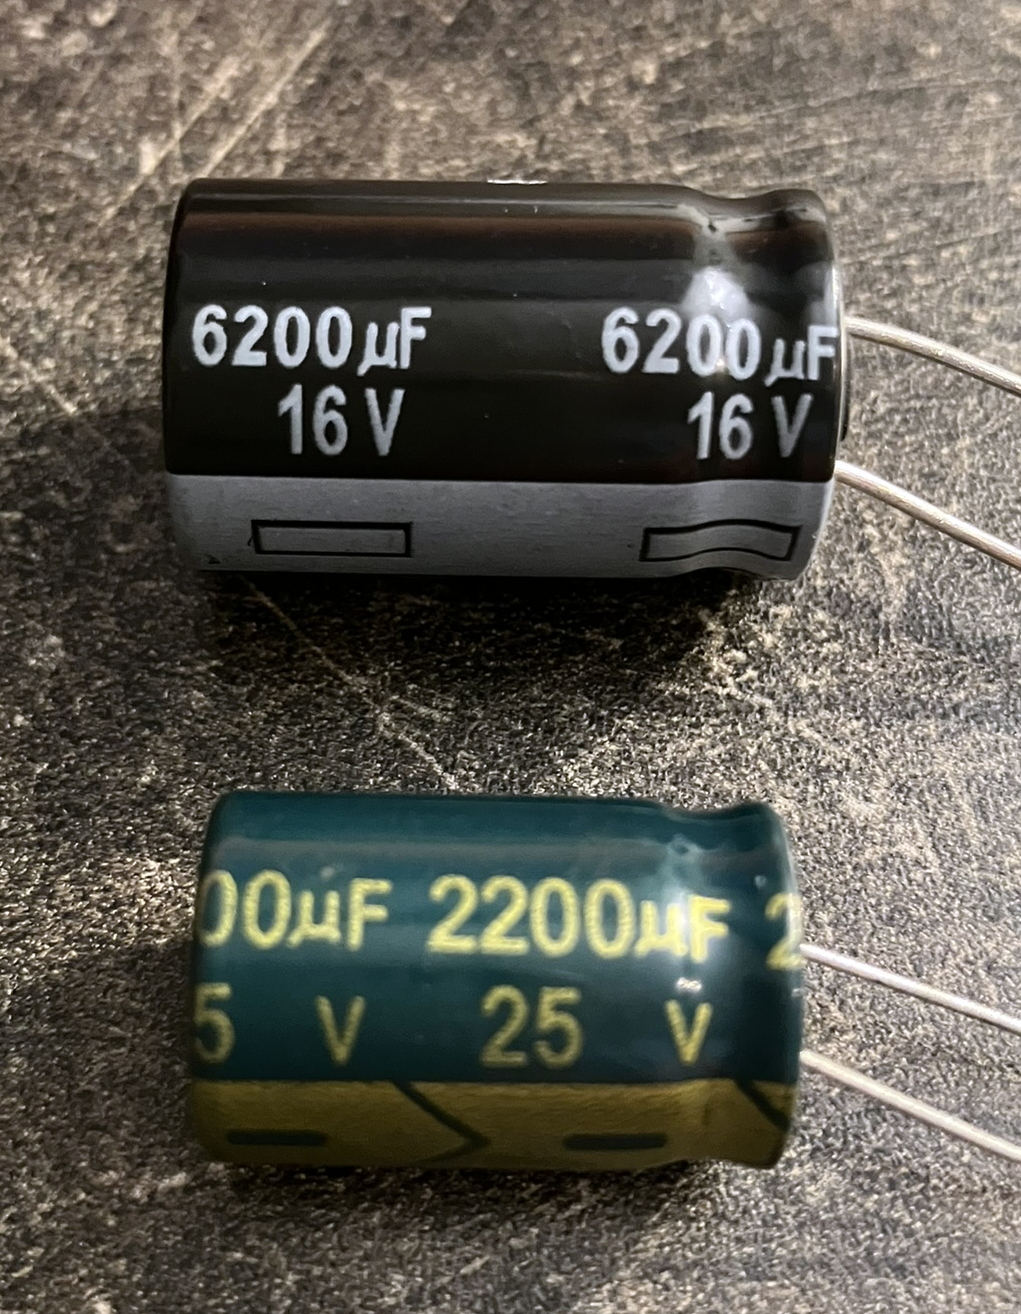
\includegraphics[width=0.85\textwidth]{foto/198}
    \caption{\scriptsize Elektrolytkondensatoren mit Markierung des Minus-Pols}
    \label{e_kondensator_elkos}
\end{figure}

   \end{column}
\end{columns}

\end{frame}

\begin{frame}
\only<1>{
\begin{QQuestion}{EC207}{Bei welcher der folgenden Bauformen von Kondensatoren muss beim Einbau auf die Polarität geachtet werden?}{Elektrolytkondensator}
{Keramikkondensator}
{Styroflexkondensator}
{Plattenkondensator}
\end{QQuestion}

}
\only<2>{
\begin{QQuestion}{EC207}{Bei welcher der folgenden Bauformen von Kondensatoren muss beim Einbau auf die Polarität geachtet werden?}{\textbf{\textcolor{DARCgreen}{Elektrolytkondensator}}}
{Keramikkondensator}
{Styroflexkondensator}
{Plattenkondensator}
\end{QQuestion}

}
\end{frame}

\begin{frame}
\frametitle{Ladekurve}
\begin{columns}
    \begin{column}{0.48\textwidth}
    \begin{itemize}
  \item Ein leerer Kondensator wird an Gleichspannung angeschlossen
  \item Die Spannung steigt steil an und flacht dann zur angelegten Spannung ab 
  \end{itemize}

    \end{column}
   \begin{column}{0.48\textwidth}
       
\begin{figure}
    \DARCimage{0.85\linewidth}{185include}
    \caption{\scriptsize Ladekurve eines Kondensators}
    \label{e_ladekurve_kondensator}
\end{figure}


   \end{column}
\end{columns}

\end{frame}

\begin{frame}
\only<1>{
\begin{question2x2}{EC201}{Welchen zeitlichen Verlauf hat die Spannung an einem entladenen Kondensator, wenn dieser über einen Widerstand an eine Gleichspannungsquelle angeschlossen wird?}{\DARCimage{1.0\linewidth}{188include}}
{\DARCimage{1.0\linewidth}{186include}}
{\DARCimage{1.0\linewidth}{185include}}
{\DARCimage{1.0\linewidth}{187include}}
\end{question2x2}

}
\only<2>{
\begin{question2x2}{EC201}{Welchen zeitlichen Verlauf hat die Spannung an einem entladenen Kondensator, wenn dieser über einen Widerstand an eine Gleichspannungsquelle angeschlossen wird?}{\DARCimage{1.0\linewidth}{188include}}
{\DARCimage{1.0\linewidth}{186include}}
{\textbf{\textcolor{DARCgreen}{\DARCimage{1.0\linewidth}{185include}}}}
{\DARCimage{1.0\linewidth}{187include}}
\end{question2x2}

}
\end{frame}

\begin{frame}
\frametitle{Kondensator im Wechselstrom}
\begin{itemize}
  \item Im Gleichstromkreis lädt der Kondensator sich auf, wirkt dann aber wie ein unendlich großer Widerstand
  \item Bei Wechselstrom wird der Kondensator ständig Auf- und Entladen
  \item Je höher die Frequenz, umso geringer ist der Wechselstromwiderstand des Kondensators
  \end{itemize}
\end{frame}

\begin{frame}
\only<1>{
\begin{QQuestion}{EC202}{Welches Verhalten zeigt der Wechselstromwiderstand eines idealen Kondensators mit zunehmender Frequenz?}{Er sinkt.}
{Er sinkt bis zu einem Minimum und steigt dann wieder.}
{Er steigt.}
{Er steigt bis zu einem Maximum und sinkt dann wieder.}
\end{QQuestion}

}
\only<2>{
\begin{QQuestion}{EC202}{Welches Verhalten zeigt der Wechselstromwiderstand eines idealen Kondensators mit zunehmender Frequenz?}{\textbf{\textcolor{DARCgreen}{Er sinkt.}}}
{Er sinkt bis zu einem Minimum und steigt dann wieder.}
{Er steigt.}
{Er steigt bis zu einem Maximum und sinkt dann wieder.}
\end{QQuestion}

}
\end{frame}%ENDCONTENT


\section{Phase}
\label{section:phase}
\begin{frame}%STARTCONTENT

\only<1>{
\begin{PQuestion}{AB302}{Welche Antwort enthält die richtigen Phasenwinkel der dargestellten sinusförmigen Wechselspannung an der mit X$_3$ bezeichneten Stelle?}{$\dfrac{3\pi}{2}; \qty{270}{\degree}$}
{$\dfrac{\pi}{3}; \qty{270}{\degree}$}
{$3\pi; \qty{180}{\degree}$}
{$\dfrac{3\pi}{4}; \qty{135}{\degree}$}
{\DARCimage{1.0\linewidth}{207include}}\end{PQuestion}

}
\only<2>{
\begin{PQuestion}{AB302}{Welche Antwort enthält die richtigen Phasenwinkel der dargestellten sinusförmigen Wechselspannung an der mit X$_3$ bezeichneten Stelle?}{\textbf{\textcolor{DARCgreen}{$\dfrac{3\pi}{2}; \qty{270}{\degree}$}}}
{$\dfrac{\pi}{3}; \qty{270}{\degree}$}
{$3\pi; \qty{180}{\degree}$}
{$\dfrac{3\pi}{4}; \qty{135}{\degree}$}
{\DARCimage{1.0\linewidth}{207include}}\end{PQuestion}

}
\end{frame}

\begin{frame}
\only<1>{
\begin{PQuestion}{AB303}{Der Betrag der Phasendifferenz zwischen den beiden in der Abbildung dargestellten Sinussignalen ist~...}{\qty{45}{\degree}. }
{\qty{0}{\degree}.}
{\qty{90}{\degree}.}
{\qty{180}{\degree}.}
{\DARCimage{1.0\linewidth}{208include}}\end{PQuestion}

}
\only<2>{
\begin{PQuestion}{AB303}{Der Betrag der Phasendifferenz zwischen den beiden in der Abbildung dargestellten Sinussignalen ist~...}{\textbf{\textcolor{DARCgreen}{\qty{45}{\degree}. }}}
{\qty{0}{\degree}.}
{\qty{90}{\degree}.}
{\qty{180}{\degree}.}
{\DARCimage{1.0\linewidth}{208include}}\end{PQuestion}

}
\end{frame}%ENDCONTENT


\section{Kondensator II}
\label{section:kondensator_2}
\begin{frame}%STARTCONTENT

\only<1>{
\begin{QQuestion}{AC101}{Ein verlustloser Kondensator wird an eine Wechselspannungsquelle angeschlossen. Welche Phasenverschiebung zwischen Spannung und Strom stellt sich ein?}{Der Strom eilt der Spannung um \qty{90}{\degree} voraus.}
{Die Spannung eilt dem Strom um \qty{90}{\degree} voraus.}
{Die Spannung eilt dem Strom um \qty{45}{\degree} voraus.}
{Der Strom eilt der Spannung um \qty{45}{\degree} voraus.}
\end{QQuestion}

}
\only<2>{
\begin{QQuestion}{AC101}{Ein verlustloser Kondensator wird an eine Wechselspannungsquelle angeschlossen. Welche Phasenverschiebung zwischen Spannung und Strom stellt sich ein?}{\textbf{\textcolor{DARCgreen}{Der Strom eilt der Spannung um \qty{90}{\degree} voraus.}}}
{Die Spannung eilt dem Strom um \qty{90}{\degree} voraus.}
{Die Spannung eilt dem Strom um \qty{45}{\degree} voraus.}
{Der Strom eilt der Spannung um \qty{45}{\degree} voraus.}
\end{QQuestion}

}
\end{frame}

\begin{frame}
\only<1>{
\begin{QQuestion}{AC102}{Welches Vorzeichen hat der Blindwiderstand eines idealen Kondensators und von welchen physikalischen Größen hängt er ab? Der Blindwiderstand ist~...}{positiv und unabhängig von der Kapazität und der anliegenden Frequenz.}
{negativ und unabhängig von der Kapazität und der anliegenden Frequenz.}
{positiv und abhängig von der Kapazität und der anliegenden Frequenz.}
{negativ und abhängig von der Kapazität und der anliegenden Frequenz.}
\end{QQuestion}

}
\only<2>{
\begin{QQuestion}{AC102}{Welches Vorzeichen hat der Blindwiderstand eines idealen Kondensators und von welchen physikalischen Größen hängt er ab? Der Blindwiderstand ist~...}{positiv und unabhängig von der Kapazität und der anliegenden Frequenz.}
{negativ und unabhängig von der Kapazität und der anliegenden Frequenz.}
{positiv und abhängig von der Kapazität und der anliegenden Frequenz.}
{\textbf{\textcolor{DARCgreen}{negativ und abhängig von der Kapazität und der anliegenden Frequenz.}}}
\end{QQuestion}

}
\end{frame}

\begin{frame}
\only<1>{
\begin{QQuestion}{AC103}{Welcher der folgenden Widerstände hat keine Wärmeverluste?}{Der NTC-Widerstand}
{Der Metalloxidwiderstand}
{Der Wirkwiderstand}
{Der Blindwiderstand}
\end{QQuestion}

}
\only<2>{
\begin{QQuestion}{AC103}{Welcher der folgenden Widerstände hat keine Wärmeverluste?}{Der NTC-Widerstand}
{Der Metalloxidwiderstand}
{Der Wirkwiderstand}
{\textbf{\textcolor{DARCgreen}{Der Blindwiderstand}}}
\end{QQuestion}

}
\end{frame}

\begin{frame}
\only<1>{
\begin{QQuestion}{AC104}{Wie groß ist der Betrag des kapazitiven Blindwiderstands eines Kondensators mit \qty{10}{\pF} bei einer Frequenz von \qty{100}{\MHz}?}{\qty{318}{\ohm}}
{\qty{1,59}{\kohm}}
{\qty{159}{\ohm}}
{\qty{31,8}{\ohm}}
\end{QQuestion}

}
\only<2>{
\begin{QQuestion}{AC104}{Wie groß ist der Betrag des kapazitiven Blindwiderstands eines Kondensators mit \qty{10}{\pF} bei einer Frequenz von \qty{100}{\MHz}?}{\qty{318}{\ohm}}
{\qty{1,59}{\kohm}}
{\textbf{\textcolor{DARCgreen}{\qty{159}{\ohm}}}}
{\qty{31,8}{\ohm}}
\end{QQuestion}

}
\end{frame}

\begin{frame}
\frametitle{Lösungsweg}
\begin{itemize}
  \item gegeben: $C = 10pF$
  \item gegeben: $f = 100MHz$
  \item gesucht: $X_{\textrm{C}}$
  \end{itemize}
    \pause
    \begin{equation}\begin{split}\nonumber X_{\textrm{C}} &= \frac{1}{\omega \cdot C} = \frac{1}{2\pi \cdot f \cdot C}\\ &= \frac{1}{2\pi \cdot 100MHz \cdot 10pF}\\ &\approx 159\Omega \end{split}\end{equation}



\end{frame}

\begin{frame}
\only<1>{
\begin{QQuestion}{AC106}{Wie groß ist der Betrag des kapazitiven Blindwiderstands eines Kondensators mit \qty{100}{\pF} bei einer Frequenz von \qty{100}{\MHz}?}{ca. \qty{15,9}{\ohm}}
{ca. \qty{159}{\ohm}}
{ca. \qty{31,8}{\ohm}}
{ca. \qty{3,2}{\ohm}}
\end{QQuestion}

}
\only<2>{
\begin{QQuestion}{AC106}{Wie groß ist der Betrag des kapazitiven Blindwiderstands eines Kondensators mit \qty{100}{\pF} bei einer Frequenz von \qty{100}{\MHz}?}{\textbf{\textcolor{DARCgreen}{ca. \qty{15,9}{\ohm}}}}
{ca. \qty{159}{\ohm}}
{ca. \qty{31,8}{\ohm}}
{ca. \qty{3,2}{\ohm}}
\end{QQuestion}

}
\end{frame}

\begin{frame}
\frametitle{Lösungsweg}
\begin{itemize}
  \item gegeben: $C = 100pF$
  \item gegeben: $f = 100MHz$
  \item gesucht: $X_{\textrm{C}}$
  \end{itemize}
    \pause
    \begin{equation}\begin{split}\nonumber X_{\textrm{C}} &= \frac{1}{\omega \cdot C} = \frac{1}{2\pi \cdot f \cdot C}\\ &= \frac{1}{2\pi \cdot 100MHz \cdot 100pF}\\ &\approx 15,9\Omega \end{split}\end{equation}



\end{frame}

\begin{frame}
\only<1>{
\begin{QQuestion}{AC105}{Wie groß ist der Betrag des kapazitiven Blindwiderstands eines Kondensators mit \qty{50}{\pF} bei einer Frequenz von \qty{145}{\MHz} ?}{ca. \qty{69}{\ohm}}
{ca. \qty{0,045}{\ohm}}
{ca. \qty{18,2}{\kohm}}
{ca. \qty{22}{\ohm}}
\end{QQuestion}

}
\only<2>{
\begin{QQuestion}{AC105}{Wie groß ist der Betrag des kapazitiven Blindwiderstands eines Kondensators mit \qty{50}{\pF} bei einer Frequenz von \qty{145}{\MHz} ?}{ca. \qty{69}{\ohm}}
{ca. \qty{0,045}{\ohm}}
{ca. \qty{18,2}{\kohm}}
{\textbf{\textcolor{DARCgreen}{ca. \qty{22}{\ohm}}}}
\end{QQuestion}

}
\end{frame}

\begin{frame}
\frametitle{Lösungsweg}
\begin{itemize}
  \item gegeben: $C = 50pF$
  \item gegeben: $f = 145MHz$
  \item gesucht: $X_{\textrm{C}}$
  \end{itemize}
    \pause
    \begin{equation}\begin{split}\nonumber X_{\textrm{C}} &= \frac{1}{\omega \cdot C} = \frac{1}{2\pi \cdot f \cdot C}\\ &= \frac{1}{2\pi \cdot 145MHz \cdot 50pF}\\ &\approx 22\Omega \end{split}\end{equation}



\end{frame}

\begin{frame}
\only<1>{
\begin{QQuestion}{AC107}{Wie groß ist der Betrag des kapazitiven Blindwiderstands eines Kondensators mit \qty{100}{\pF} bei einer Frequenz von \qty{435}{\MHz} ?}{ca. \qty{3,7}{\ohm}}
{ca. \qty{0,27}{\ohm}}
{ca. \qty{27,3}{\kohm}}
{ca. \qty{11,5}{\ohm}}
\end{QQuestion}

}
\only<2>{
\begin{QQuestion}{AC107}{Wie groß ist der Betrag des kapazitiven Blindwiderstands eines Kondensators mit \qty{100}{\pF} bei einer Frequenz von \qty{435}{\MHz} ?}{\textbf{\textcolor{DARCgreen}{ca. \qty{3,7}{\ohm}}}}
{ca. \qty{0,27}{\ohm}}
{ca. \qty{27,3}{\kohm}}
{ca. \qty{11,5}{\ohm}}
\end{QQuestion}

}
\end{frame}

\begin{frame}
\frametitle{Lösungsweg}
\begin{itemize}
  \item gegeben: $C = 100pF$
  \item gegeben: $f = 435MHz$
  \item gesucht: $X_{\textrm{C}}$
  \end{itemize}
    \pause
    \begin{equation}\begin{split}\nonumber X_{\textrm{C}} &= \frac{1}{\omega \cdot C} = \frac{1}{2\pi \cdot f \cdot C}\\ &= \frac{1}{2\pi \cdot 435MHz \cdot 100pF}\\ &\approx 3,7\Omega \end{split}\end{equation}



\end{frame}

\begin{frame}
\only<1>{
\begin{QQuestion}{AC108}{An einem unbekannten Kondensator liegt eine Wechselspannung mit \qty{16}{\V} und \qty{50}{\Hz}. Es wird ein Strom von \qty{32}{\mA} gemessen. Welche Kapazität hat der Kondensator?}{ca. \qty{0,637}{\micro\F}}
{ca. \qty{6,37}{\micro\F}}
{ca. \qty{0,45}{\micro\F}}
{ca. \qty{4,5}{\micro\F}}
\end{QQuestion}

}
\only<2>{
\begin{QQuestion}{AC108}{An einem unbekannten Kondensator liegt eine Wechselspannung mit \qty{16}{\V} und \qty{50}{\Hz}. Es wird ein Strom von \qty{32}{\mA} gemessen. Welche Kapazität hat der Kondensator?}{ca. \qty{0,637}{\micro\F}}
{\textbf{\textcolor{DARCgreen}{ca. \qty{6,37}{\micro\F}}}}
{ca. \qty{0,45}{\micro\F}}
{ca. \qty{4,5}{\micro\F}}
\end{QQuestion}

}
\end{frame}

\begin{frame}
\frametitle{Lösungsweg}
\begin{columns}
    \begin{column}{0.48\textwidth}
    \begin{itemize}
  \item gegeben: $U = 16V$
  \item gegeben: $I = 32mA$
  \end{itemize}

    \end{column}
   \begin{column}{0.48\textwidth}
       \begin{itemize}
  \item gegeben: $f = 50Hz$
  \item gesucht: $C$
  \end{itemize}

   \end{column}
\end{columns}
    \pause
    $X_{\textrm{C}} = \frac{U}{I} = \frac{16V}{32mA} = 500\Omega$
    \pause
    \begin{equation}\begin{align}\nonumber X_{\textrm{C}} &= \frac{1}{\omega \cdot C} \\ \nonumber \Rightarrow C &= \frac{1}{\omega \cdot X_{\textrm{C}}} = \frac{1}{2\pi \cdot f \cdot X_{\textrm{C}}}\\ \nonumber &= \frac{1}{2\pi \cdot 50Hz \cdot 500\Omega}\\ \nonumber &\approx 6,37\mu F\end{align}\end{equation}



\end{frame}

\begin{frame}
\only<1>{
\begin{QQuestion}{AC109}{Kommt es in einem von Wechselstrom durchflossenen realen Kondensator zu Verlusten?}{Ja, infolge von Verlusten in Dielektrikum und Zuleitung}
{Nein, beim Kondensator handelt es sich  um eine reine Blindleistung.}
{Ja, infolge des Blindwiderstands}
{Nein, bei Wechselstrom treten keine Verluste auf.}
\end{QQuestion}

}
\only<2>{
\begin{QQuestion}{AC109}{Kommt es in einem von Wechselstrom durchflossenen realen Kondensator zu Verlusten?}{\textbf{\textcolor{DARCgreen}{Ja, infolge von Verlusten in Dielektrikum und Zuleitung}}}
{Nein, beim Kondensator handelt es sich  um eine reine Blindleistung.}
{Ja, infolge des Blindwiderstands}
{Nein, bei Wechselstrom treten keine Verluste auf.}
\end{QQuestion}

}
\end{frame}

\begin{frame}
\only<1>{
\begin{QQuestion}{AC110}{Neben dem kapazitiven Blindwiderstand treten im von Wechselstrom durchflossenen Kondensator auch Verluste auf, die rechnerisch in einem parallelgeschalteten Verlustwiderstand zusammengefasst werden können. Die Kondensatorverluste werden oft durch~...}{den relativen Blindwiderstand in Ohm pro Farad angegeben, mit dem die Kondensatorgüte berechnet werden kann.}
{den relativen Verlustwiderstand in Ohm pro Farad angegeben, mit dem die Kondensatorgüte berechnet werden kann.}
{den Verlustfaktor tan $\delta$ angegeben, der dem Kehrwert des Gütefaktors entspricht.}
{den Verlustfaktor cos $\phi$ angegeben, der dem Kehrwert des Gütefaktors entspricht.}
\end{QQuestion}

}
\only<2>{
\begin{QQuestion}{AC110}{Neben dem kapazitiven Blindwiderstand treten im von Wechselstrom durchflossenen Kondensator auch Verluste auf, die rechnerisch in einem parallelgeschalteten Verlustwiderstand zusammengefasst werden können. Die Kondensatorverluste werden oft durch~...}{den relativen Blindwiderstand in Ohm pro Farad angegeben, mit dem die Kondensatorgüte berechnet werden kann.}
{den relativen Verlustwiderstand in Ohm pro Farad angegeben, mit dem die Kondensatorgüte berechnet werden kann.}
{\textbf{\textcolor{DARCgreen}{den Verlustfaktor tan $\delta$ angegeben, der dem Kehrwert des Gütefaktors entspricht.}}}
{den Verlustfaktor cos $\phi$ angegeben, der dem Kehrwert des Gütefaktors entspricht.}
\end{QQuestion}

}
\end{frame}

\begin{frame}
\only<1>{
\begin{QQuestion}{AC111}{An einem Kondensator mit einer Kapazität von \qty{1}{\micro\F} wird ein NF-Signal mit \qty{10}{\kHz} und \qty{12}{\V}$_{\textrm{eff}}$ angelegt. Wie groß ist die aufgenommene Wirkleistung im eingeschwungenen Zustand?}{\qty{0,9}{\W}}
{Näherungsweise \qty{0}{\W}}
{\qty{0,75}{\W}}
{\qty{9}{\W}}
\end{QQuestion}

}
\only<2>{
\begin{QQuestion}{AC111}{An einem Kondensator mit einer Kapazität von \qty{1}{\micro\F} wird ein NF-Signal mit \qty{10}{\kHz} und \qty{12}{\V}$_{\textrm{eff}}$ angelegt. Wie groß ist die aufgenommene Wirkleistung im eingeschwungenen Zustand?}{\qty{0,9}{\W}}
{\textbf{\textcolor{DARCgreen}{Näherungsweise \qty{0}{\W}}}}
{\qty{0,75}{\W}}
{\qty{9}{\W}}
\end{QQuestion}

}

\end{frame}%ENDCONTENT


\section{Spule I}
\label{section:spule_1}
\begin{frame}%STARTCONTENT

\frametitle{Induktivität}
\begin{columns}
    \begin{column}{0.48\textwidth}
    \begin{itemize}
  \item Jeder stromdurchflossene Leiter hat eine Induktivität
  \item Um einen stromdurchflossenen Leiter entsteht ein Magnetfeld
  \item In einem Leiter entsteht ein Strom, wenn dieser durch ein Magnetfeld bewegt wird
  \end{itemize}

    \end{column}
   \begin{column}{0.48\textwidth}
       
\begin{figure}
    \DARCimage{0.85\linewidth}{833include}
    \caption{\scriptsize Magnetfeld um einen stromdurchflossenen Leiter}
    \label{e_spule_magnetfeld_um_leiter}
\end{figure}


   \end{column}
\end{columns}

\end{frame}

\begin{frame}
\only<1>{
\begin{QQuestion}{EC304}{Hat ein gerades Leiterstück eine Induktivität?}{Nein, der Leiter muss wenigstens eine Krümmung (eine viertel, halbe oder ganze Windung) haben.}
{Ja, jeder Leiter besitzt, unabhängig von der Form, eine Induktivität.}
{Ja, solange der Blindwiderstand \qty{0}{\ohm} beträgt.}
{Nein, beispielsweise im Vakuum entstehen keine Induktivitäten.}
\end{QQuestion}

}
\only<2>{
\begin{QQuestion}{EC304}{Hat ein gerades Leiterstück eine Induktivität?}{Nein, der Leiter muss wenigstens eine Krümmung (eine viertel, halbe oder ganze Windung) haben.}
{\textbf{\textcolor{DARCgreen}{Ja, jeder Leiter besitzt, unabhängig von der Form, eine Induktivität.}}}
{Ja, solange der Blindwiderstand \qty{0}{\ohm} beträgt.}
{Nein, beispielsweise im Vakuum entstehen keine Induktivitäten.}
\end{QQuestion}

}
\end{frame}

\begin{frame}
\frametitle{Spule und Induktivität}
\begin{itemize}
  \item Eine Spule optimiert die Induktivität eines Leiters
  \item Wichtigste Eigenschaft der Spule: Energie speichern
  \end{itemize}
$L = \dfrac{N\cdot \Phi}{I}$

\begin{itemize}
  \item mit $N$ Anzahl Windungen und $\Phi$ als magnetischer Fluss
  \item Einheit: $\frac{Vs}{A}$ bzw. Henry $H$
  \item Die Induktivität ist der magnetische Fluss pro Ampere
  \end{itemize}

\end{frame}

\begin{frame}
\frametitle{Induktivität durch Bauart}
\begin{columns}
    \begin{column}{0.48\textwidth}
    \begin{itemize}
  \item Die Induktivität einer Spule kann durch die Bauart erreicht werden
  \end{itemize}
$L = \dfrac{\mu_0 \cdot \mu_r \cdot N^2 \cdot A_S}{l}$

\begin{itemize}
  \item $\rightarrow$ Induktivität ist größer bei größerem Querschnitt, anderem Kern oder kleinerer Länge
  \item $\rightarrow$ Induktivität ist viel größer bei höherer Windungszahl
  \end{itemize}

    \end{column}
   \begin{column}{0.48\textwidth}
       \begin{itemize}
  \item $\mu_0 = 1,2566 \cdot 10^{-6}\frac{H}{m}$: magnetische Feldkonstante
  \item $\mu_r$: relative Permeabilität, abhängig vom Spulenkern (Luft  $\approx$  1)
  \item $N$: Windungszahl
  \item $A_S$: Querschnittsfläche der Spule
  \item $l$: Länge der Spule bzw. mittlere Feldlinienlänge
  \end{itemize}

   \end{column}
\end{columns}

\end{frame}

\begin{frame}
\only<1>{
\begin{QQuestion}{EA102}{Welche Einheit wird üblicherweise für die Induktivität verwendet?}{Henry (H)}
{Farad (F)}
{Ohm ($\Omega$)}
{Amperestunden (Ah)}
\end{QQuestion}

}
\only<2>{
\begin{QQuestion}{EA102}{Welche Einheit wird üblicherweise für die Induktivität verwendet?}{\textbf{\textcolor{DARCgreen}{Henry (H)}}}
{Farad (F)}
{Ohm ($\Omega$)}
{Amperestunden (Ah)}
\end{QQuestion}

}
\end{frame}

\begin{frame}
\only<1>{
\begin{PQuestion}{EC307}{Wie ändert sich die Induktivität einer Spule von \qty{12}{\micro\H}, wenn die Windungszahl bei gleicher Wickellänge verdoppelt wird?}{Die Induktivität steigt auf \qty{24}{\micro\H}.}
{Die Induktivität steigt auf \qty{48}{\micro\H}.}
{Die Induktivität sinkt auf \qty{6}{\micro\H}.}
{Die Induktivität sinkt auf \qty{3}{\micro\H}.}
{\DARCimage{1.0\linewidth}{449include}}\end{PQuestion}

}
\only<2>{
\begin{PQuestion}{EC307}{Wie ändert sich die Induktivität einer Spule von \qty{12}{\micro\H}, wenn die Windungszahl bei gleicher Wickellänge verdoppelt wird?}{Die Induktivität steigt auf \qty{24}{\micro\H}.}
{\textbf{\textcolor{DARCgreen}{Die Induktivität steigt auf \qty{48}{\micro\H}.}}}
{Die Induktivität sinkt auf \qty{6}{\micro\H}.}
{Die Induktivität sinkt auf \qty{3}{\micro\H}.}
{\DARCimage{1.0\linewidth}{449include}}\end{PQuestion}

}
\end{frame}

\begin{frame}
\only<1>{
\begin{PQuestion}{EC306}{Vorausgesetzt sind zwei Spulen in gleicher Umgebung, mit gleicher Windungszahl und mit gleicher Querschnittsfläche. Die erste Spule hat eine Induktivität von \qty{12}{\micro\H}. Die zweite Spule hat die doppelte Länge der ersten Spule. Wie hoch ist die Induktivität der zweiten Spule?}{\qty{3}{\micro\H}}
{\qty{24}{\micro\H}}
{\qty{48}{\micro\H}}
{\qty{6}{\micro\H}}
{\DARCimage{1.0\linewidth}{473include}}\end{PQuestion}

}
\only<2>{
\begin{PQuestion}{EC306}{Vorausgesetzt sind zwei Spulen in gleicher Umgebung, mit gleicher Windungszahl und mit gleicher Querschnittsfläche. Die erste Spule hat eine Induktivität von \qty{12}{\micro\H}. Die zweite Spule hat die doppelte Länge der ersten Spule. Wie hoch ist die Induktivität der zweiten Spule?}{\qty{3}{\micro\H}}
{\qty{24}{\micro\H}}
{\qty{48}{\micro\H}}
{\textbf{\textcolor{DARCgreen}{\qty{6}{\micro\H}}}}
{\DARCimage{1.0\linewidth}{473include}}\end{PQuestion}

}
\end{frame}

\begin{frame}
\only<1>{
\begin{QQuestion}{EC305}{Wie kann man die Induktivität einer zylindrischen Spule vergrößern?}{Durch Einführen eines Kupferkerns in die Spule.}
{Durch Auseinanderziehen der Spule in Längsrichtung.}
{Durch Stauchen der Spule in Längsrichtung.}
{Durch Einbau der Spule in einen Abschirmbecher.}
\end{QQuestion}

}
\only<2>{
\begin{QQuestion}{EC305}{Wie kann man die Induktivität einer zylindrischen Spule vergrößern?}{Durch Einführen eines Kupferkerns in die Spule.}
{Durch Auseinanderziehen der Spule in Längsrichtung.}
{\textbf{\textcolor{DARCgreen}{Durch Stauchen der Spule in Längsrichtung.}}}
{Durch Einbau der Spule in einen Abschirmbecher.}
\end{QQuestion}

}
\end{frame}

\begin{frame}
\frametitle{Stromfluss über eine Spule}
\begin{columns}
    \begin{column}{0.48\textwidth}
    \begin{itemize}
  \item Strom braucht länger durch die Spule
  \item Erst leuchtet Lampe<sub>1</sub>
  \item Später leuchtet Lampe<sub>2</sub>
  \end{itemize}

    \end{column}
   \begin{column}{0.48\textwidth}
       
\begin{figure}
    \DARCimage{0.85\linewidth}{541include}
    \caption{\scriptsize Stromkreis mit Spule}
    \label{e_stromkreis_mit_spule}
\end{figure}


   \end{column}
\end{columns}

\end{frame}

\begin{frame}
\only<1>{
\begin{PQuestion}{EC302}{Schaltet man zwei Leuchtmittel gleichzeitig an eine Gleichspannungsquelle, wobei ein Leuchtmittel, Lampe 1, zum Helligkeitsausgleich über einen Widerstand und das andere, Lampe 2, über eine Spule mit vielen Windungen und Eisenkern angeschlossen ist, so~...}{leuchtet Lampe 2 zuerst.}
{leuchtet Lampe 1 zuerst.}
{leuchten Lampe 1 und Lampe 2 genau gleichzeitig.}
{leuchtet Lampe 2 kurz auf und geht wieder aus. Lampe 1 leuchtet.}
{\DARCimage{1.0\linewidth}{541include}}\end{PQuestion}

}
\only<2>{
\begin{PQuestion}{EC302}{Schaltet man zwei Leuchtmittel gleichzeitig an eine Gleichspannungsquelle, wobei ein Leuchtmittel, Lampe 1, zum Helligkeitsausgleich über einen Widerstand und das andere, Lampe 2, über eine Spule mit vielen Windungen und Eisenkern angeschlossen ist, so~...}{leuchtet Lampe 2 zuerst.}
{\textbf{\textcolor{DARCgreen}{leuchtet Lampe 1 zuerst.}}}
{leuchten Lampe 1 und Lampe 2 genau gleichzeitig.}
{leuchtet Lampe 2 kurz auf und geht wieder aus. Lampe 1 leuchtet.}
{\DARCimage{1.0\linewidth}{541include}}\end{PQuestion}

}
\end{frame}

\begin{frame}
\frametitle{Einschaltkurve Spule}
\begin{columns}
    \begin{column}{0.48\textwidth}
    \begin{itemize}
  \item Eine Spule wird an Gleichspannung angeschlossen
  \item Die Spannung nimmt steil ab und gleicht sich mit der Zeit 0 an
  \end{itemize}

    \end{column}
   \begin{column}{0.48\textwidth}
       
\begin{figure}
    \DARCimage{0.85\linewidth}{186include}
    \caption{\scriptsize Zeitlicher Verlauf einer Gleichspannung über eine Spule}
    \label{e_einschaltkurve_spule}
\end{figure}


   \end{column}
\end{columns}

\end{frame}

\begin{frame}
\only<1>{
\begin{question2x2}{EC301}{An eine Spule wird über einen Widerstand eine Gleichspannung angelegt. Welches der nachfolgenden Diagramme zeigt den zeitlichen Verlauf der Spannung über der Spule?}{\DARCimage{1.0\linewidth}{185include}}
{\DARCimage{1.0\linewidth}{186include}}
{\DARCimage{1.0\linewidth}{188include}}
{\DARCimage{1.0\linewidth}{187include}}
\end{question2x2}

}
\only<2>{
\begin{question2x2}{EC301}{An eine Spule wird über einen Widerstand eine Gleichspannung angelegt. Welches der nachfolgenden Diagramme zeigt den zeitlichen Verlauf der Spannung über der Spule?}{\DARCimage{1.0\linewidth}{185include}}
{\textbf{\textcolor{DARCgreen}{\DARCimage{1.0\linewidth}{186include}}}}
{\DARCimage{1.0\linewidth}{188include}}
{\DARCimage{1.0\linewidth}{187include}}
\end{question2x2}

}
\end{frame}

\begin{frame}
\frametitle{Spule im Wechselstrom}
\begin{itemize}
  \item Im Gleichstromkreis wirkt eine Spule erst wie ein unendlich großer Widerstand, wird dann aber nach dem Einschaltvorgang so groß wie der Widerstand des Leiters
  \item Bei Wechselstrom wird das Magnetfeld in der Spule ständig umgepolt
  \item Dadurch entsteht eine Selbstinduktionspannung, die entgegengerichtet ist und stört
  \item Je höher die Frequenz, umso höher ist der Wechselstromwiderstand der Spule
  \end{itemize}
\end{frame}

\begin{frame}
\only<1>{
\begin{QQuestion}{EC303}{Welches Verhalten zeigt der Wechselstromwiderstand einer idealen Spule mit zunehmender Frequenz?}{Er steigt.}
{Er sinkt.}
{Er sinkt bis zu einem Minimum und steigt dann wieder.}
{Er steigt bis zu einem Maximum und sinkt dann wieder.}
\end{QQuestion}

}
\only<2>{
\begin{QQuestion}{EC303}{Welches Verhalten zeigt der Wechselstromwiderstand einer idealen Spule mit zunehmender Frequenz?}{\textbf{\textcolor{DARCgreen}{Er steigt.}}}
{Er sinkt.}
{Er sinkt bis zu einem Minimum und steigt dann wieder.}
{Er steigt bis zu einem Maximum und sinkt dann wieder.}
\end{QQuestion}

}
\end{frame}%ENDCONTENT


\section{Spule II}
\label{section:spule_2}
\begin{frame}%STARTCONTENT

\only<1>{
\begin{QQuestion}{AA101}{Welche Einheit wird üblicherweise für die Impedanz verwendet?}{Farad}
{Ohm}
{Siemens}
{Henry}
\end{QQuestion}

}
\only<2>{
\begin{QQuestion}{AA101}{Welche Einheit wird üblicherweise für die Impedanz verwendet?}{Farad}
{\textbf{\textcolor{DARCgreen}{Ohm}}}
{Siemens}
{Henry}
\end{QQuestion}

}
\end{frame}

\begin{frame}
\only<1>{
\begin{QQuestion}{AC201}{In einer idealen Induktivität, die an einer Wechselspannungsquelle angeschlossen ist, eilt der Strom der angelegten Spannung~...}{um \qty{45}{\degree} voraus.}
{um \qty{90}{\degree} nach.}
{um \qty{45}{\degree} nach.}
{um \qty{90}{\degree} voraus.}
\end{QQuestion}

}
\only<2>{
\begin{QQuestion}{AC201}{In einer idealen Induktivität, die an einer Wechselspannungsquelle angeschlossen ist, eilt der Strom der angelegten Spannung~...}{um \qty{45}{\degree} voraus.}
{\textbf{\textcolor{DARCgreen}{um \qty{90}{\degree} nach.}}}
{um \qty{45}{\degree} nach.}
{um \qty{90}{\degree} voraus.}
\end{QQuestion}

}
\end{frame}

\begin{frame}
\only<1>{
\begin{QQuestion}{AC202}{Welches Vorzeichen hat der Blindwiderstand einer idealen Spule und von welchen physikalischen Größen hängt er ab? Der Blindwiderstand ist~...}{negativ und abhängig von der Induktivität und der anliegenden Frequenz.}
{positiv und unabhängig von der Induktivität und der anliegenden Frequenz.}
{positiv und abhängig von der Induktivität und der anliegenden Frequenz.}
{negativ und unabhängig von der Induktivität und der anliegenden Frequenz.}
\end{QQuestion}

}
\only<2>{
\begin{QQuestion}{AC202}{Welches Vorzeichen hat der Blindwiderstand einer idealen Spule und von welchen physikalischen Größen hängt er ab? Der Blindwiderstand ist~...}{negativ und abhängig von der Induktivität und der anliegenden Frequenz.}
{positiv und unabhängig von der Induktivität und der anliegenden Frequenz.}
{\textbf{\textcolor{DARCgreen}{positiv und abhängig von der Induktivität und der anliegenden Frequenz.}}}
{negativ und unabhängig von der Induktivität und der anliegenden Frequenz.}
\end{QQuestion}

}
\end{frame}

\begin{frame}
\only<1>{
\begin{QQuestion}{AC203}{Beim Anlegen einer Gleichspannung $U$ = \qty{1}{\V} an eine Spule messen Sie einen Strom. Wird der Strom beim Anlegen von einer Wechselspannung mit $U_{\symup{eff}}$ = \qty{1}{\V} größer oder kleiner?}{Beim Betrieb mit Gleichspannung wirkt nur der Gleichstromwiderstand der Spule. Beim Betrieb mit Wechselspannung wird der induktive Widerstand $X_{\symup{L}}$ wirksam und erhöht den Gesamtwiderstand. Der Strom wird kleiner.}
{Beim Betrieb mit Gleichspannung wirkt nur der Gleichstromwiderstand der Spule. Beim Betrieb mit Wechselspannung wirkt nur der kleinere induktive Widerstand $X_{\symup{L}}$. Der Strom wird größer.}
{Beim Betrieb mit Gleich- oder Wechselspannung wirkt nur der ohmsche Widerstand $X_{\symup{L}}$ der Spule. Der Strom bleibt gleich.}
{Beim Betrieb mit Wechselspannung wirkt nur der Wechselstromwiderstand der Spule. Beim Betrieb mit Gleichspannung wird nur der ohmsche Widerstand $X_{\symup{L}}$ wirksam. Der Strom wird größer.}
\end{QQuestion}

}
\only<2>{
\begin{QQuestion}{AC203}{Beim Anlegen einer Gleichspannung $U$ = \qty{1}{\V} an eine Spule messen Sie einen Strom. Wird der Strom beim Anlegen von einer Wechselspannung mit $U_{\symup{eff}}$ = \qty{1}{\V} größer oder kleiner?}{\textbf{\textcolor{DARCgreen}{Beim Betrieb mit Gleichspannung wirkt nur der Gleichstromwiderstand der Spule. Beim Betrieb mit Wechselspannung wird der induktive Widerstand $X_{\symup{L}}$ wirksam und erhöht den Gesamtwiderstand. Der Strom wird kleiner.}}}
{Beim Betrieb mit Gleichspannung wirkt nur der Gleichstromwiderstand der Spule. Beim Betrieb mit Wechselspannung wirkt nur der kleinere induktive Widerstand $X_{\symup{L}}$. Der Strom wird größer.}
{Beim Betrieb mit Gleich- oder Wechselspannung wirkt nur der ohmsche Widerstand $X_{\symup{L}}$ der Spule. Der Strom bleibt gleich.}
{Beim Betrieb mit Wechselspannung wirkt nur der Wechselstromwiderstand der Spule. Beim Betrieb mit Gleichspannung wird nur der ohmsche Widerstand $X_{\symup{L}}$ wirksam. Der Strom wird größer.}
\end{QQuestion}

}
\end{frame}

\begin{frame}
\only<1>{
\begin{QQuestion}{AC204}{Wie groß ist der Betrag des induktiven Blindwiderstands einer Spule mit \qty{3}{\micro\H} Induktivität bei einer Frequenz von \qty{100}{\MHz}?}{ca. \qty{1885}{\ohm}}
{ca. \qty{942,0}{\ohm}}
{ca. \qty{1885}{\kohm}}
{ca. \qty{1,942}{\ohm}}
\end{QQuestion}

}
\only<2>{
\begin{QQuestion}{AC204}{Wie groß ist der Betrag des induktiven Blindwiderstands einer Spule mit \qty{3}{\micro\H} Induktivität bei einer Frequenz von \qty{100}{\MHz}?}{\textbf{\textcolor{DARCgreen}{ca. \qty{1885}{\ohm}}}}
{ca. \qty{942,0}{\ohm}}
{ca. \qty{1885}{\kohm}}
{ca. \qty{1,942}{\ohm}}
\end{QQuestion}

}
\end{frame}

\begin{frame}
\frametitle{Lösungsweg}
\begin{itemize}
  \item gegeben: $L = 3\mu H$
  \item gegeben: $f = 100MHz$
  \item gesucht: $X_{\textrm{L}}$
  \end{itemize}
    \pause
    \begin{equation}\begin{split}\nonumber X_{\textrm{L}} &= \omega \cdot L = 2\pi \cdot f \cdot L\\ &= 2\pi \cdot 100MHz \cdot 3\mu H\\ &\approx 1885\Omega \end{split}\end{equation}



\end{frame}

\begin{frame}
\only<1>{
\begin{QQuestion}{AC205}{Wie groß ist die Induktivität einer Spule mit 14 Windungen, die auf einen Kern mit einer Induktivitätskonstante ($A_{\symup{L}}$-Wert) von \qty{1,5}{\nano\H} gewickelt ist?}{\qty{0,294}{\micro\H}}
{\qty{2,94}{\micro\H}}
{\qty{29,4}{\nano\H}}
{\qty{2,94}{\nano\H}}
\end{QQuestion}

}
\only<2>{
\begin{QQuestion}{AC205}{Wie groß ist die Induktivität einer Spule mit 14 Windungen, die auf einen Kern mit einer Induktivitätskonstante ($A_{\symup{L}}$-Wert) von \qty{1,5}{\nano\H} gewickelt ist?}{\textbf{\textcolor{DARCgreen}{\qty{0,294}{\micro\H}}}}
{\qty{2,94}{\micro\H}}
{\qty{29,4}{\nano\H}}
{\qty{2,94}{\nano\H}}
\end{QQuestion}

}
\end{frame}

\begin{frame}
\frametitle{Lösungsweg}
\begin{itemize}
  \item gegeben: $N = 14$
  \item gegeben: $A_{\textrm{L}} = 1,5nH$
  \item gesucht: $L$
  \end{itemize}
    \pause
    \begin{equation}\begin{split}\nonumber L &= N^2 \cdot A_{\textrm{L}}\\ &= 14^2 \cdot 1,5nH\\ &= 0,294\mu H \end{split}\end{equation}



\end{frame}

\begin{frame}
\only<1>{
\begin{QQuestion}{AC206}{Wie groß ist die Induktivität einer Spule mit 300 Windungen, die auf einen Kern mit einer Induktivitätskonstante ($A_{\symup{L}}$-Wert) von \qty{1250}{\nano\H} gewickelt ist?}{\qty{112,5}{\mH}}
{\qty{112,5}{\micro\H}}
{\qty{11,25}{\mH}}
{\qty{1,125}{\mH}}
\end{QQuestion}

}
\only<2>{
\begin{QQuestion}{AC206}{Wie groß ist die Induktivität einer Spule mit 300 Windungen, die auf einen Kern mit einer Induktivitätskonstante ($A_{\symup{L}}$-Wert) von \qty{1250}{\nano\H} gewickelt ist?}{\textbf{\textcolor{DARCgreen}{\qty{112,5}{\mH}}}}
{\qty{112,5}{\micro\H}}
{\qty{11,25}{\mH}}
{\qty{1,125}{\mH}}
\end{QQuestion}

}
\end{frame}

\begin{frame}
\frametitle{Lösungsweg}
\begin{itemize}
  \item gegeben: $N = 300$
  \item gegeben: $A_{\textrm{L}} = 1250nH$
  \item gesucht: $L$
  \end{itemize}
    \pause
    \begin{equation}\begin{split}\nonumber L &= N^2 \cdot A_{\textrm{L}}\\ &= 300^2 \cdot 1250nH\\ &= 112,5mH \end{split}\end{equation}



\end{frame}

\begin{frame}
\only<1>{
\begin{QQuestion}{AC207}{Mit einem Ringkern, dessen Induktivitätskonstante ($A_{\symup{L}}$-Wert) mit \qty{250}{\nano\H} angegeben ist, soll eine Spule mit einer Induktivität von \qty{2}{\mH} hergestellt werden. Wie groß ist die erforderliche Windungszahl etwa?}{89}
{3}
{2828}
{53}
\end{QQuestion}

}
\only<2>{
\begin{QQuestion}{AC207}{Mit einem Ringkern, dessen Induktivitätskonstante ($A_{\symup{L}}$-Wert) mit \qty{250}{\nano\H} angegeben ist, soll eine Spule mit einer Induktivität von \qty{2}{\mH} hergestellt werden. Wie groß ist die erforderliche Windungszahl etwa?}{\textbf{\textcolor{DARCgreen}{89}}}
{3}
{2828}
{53}
\end{QQuestion}

}
\end{frame}

\begin{frame}
\frametitle{Lösungsweg}
\begin{itemize}
  \item gegeben: $L = 2mH$
  \item gegeben: $A_{\textrm{L}} = 250nH$
  \item gesucht: $N$
  \end{itemize}
    \pause
    \begin{equation}\begin{align}\nonumber L &= N^2 \cdot A_{\textrm{L}}\\ \nonumber N &= \sqrt{\frac{L}{A_{\textrm{L}}}} = \sqrt{\frac{2mH}{250nH}} \\ \nonumber &= 89\ \textrm{Windungen} \end{align}\end{equation}



\end{frame}

\begin{frame}
\only<1>{
\begin{QQuestion}{AC208}{Ein Spulenkern hat eine Induktivitätskonstante ($A_{\symup{L}}$-Wert) von \qty{30}{\nano\H}. Wie groß ist die erforderliche Windungszahl zur Herstellung einer Induktivität von \qty{12}{\micro\H} in etwa?}{400}
{20}
{360}
{6}
\end{QQuestion}

}
\only<2>{
\begin{QQuestion}{AC208}{Ein Spulenkern hat eine Induktivitätskonstante ($A_{\symup{L}}$-Wert) von \qty{30}{\nano\H}. Wie groß ist die erforderliche Windungszahl zur Herstellung einer Induktivität von \qty{12}{\micro\H} in etwa?}{400}
{\textbf{\textcolor{DARCgreen}{20}}}
{360}
{6}
\end{QQuestion}

}
\end{frame}

\begin{frame}
\frametitle{Lösungsweg}
\begin{itemize}
  \item gegeben: $L = 12\mu H$
  \item gegeben: $A_{\textrm{L}} = 30nH$
  \item gesucht: $N$
  \end{itemize}
    \pause
    \begin{equation}\begin{align}\nonumber L &= N^2 \cdot A_{\textrm{L}}\\ \nonumber N &= \sqrt{\frac{L}{A_{\textrm{L}}}} = \sqrt{\frac{12\mu H}{30nH}} \\ \nonumber &= 20\ \textrm{Windungen} \end{align}\end{equation}



\end{frame}

\begin{frame}
\only<1>{
\begin{QQuestion}{AC209}{Neben dem induktiven Blindwiderstand treten in der mit Wechselstrom durchflossenen Spule auch Verluste auf, die rechnerisch in einem seriellen Verlustwiderstand zusammengefasst werden können. Als Maß für die Verluste in einer Spule wird auch~...}{der Verlustfaktor tan $\delta$ angegeben, der dem Kehrwert des Gütefaktors entspricht.}
{der relative Verlustwiderstand in Ohm pro Henry angegeben, mit dem die Spulengüte berechnet werden kann.}
{der relative Blindwiderstand in Ohm pro Henry angegeben, mit dem die Spulengüte berechnet werden kann.}
{der Verlustfaktor cos $\varphi$ angegeben, der dem Kehrwert des Gütefaktors entspricht.}
\end{QQuestion}

}
\only<2>{
\begin{QQuestion}{AC209}{Neben dem induktiven Blindwiderstand treten in der mit Wechselstrom durchflossenen Spule auch Verluste auf, die rechnerisch in einem seriellen Verlustwiderstand zusammengefasst werden können. Als Maß für die Verluste in einer Spule wird auch~...}{\textbf{\textcolor{DARCgreen}{der Verlustfaktor tan $\delta$ angegeben, der dem Kehrwert des Gütefaktors entspricht.}}}
{der relative Verlustwiderstand in Ohm pro Henry angegeben, mit dem die Spulengüte berechnet werden kann.}
{der relative Blindwiderstand in Ohm pro Henry angegeben, mit dem die Spulengüte berechnet werden kann.}
{der Verlustfaktor cos $\varphi$ angegeben, der dem Kehrwert des Gütefaktors entspricht.}
\end{QQuestion}

}
\end{frame}

\begin{frame}
\only<1>{
\begin{QQuestion}{AC210}{Um die Abstrahlungen der Spule eines abgestimmten Schwingkreises zu verringern, sollte die Spule~...}{einen abgestimmten Kunststoffkern aufweisen.}
{einen hohlen Kupferkern aufweisen.}
{in einem isolierenden Kunststoffgehäuse untergebracht werden.}
{in einem leitenden Metallgehäuse untergebracht werden.}
\end{QQuestion}

}
\only<2>{
\begin{QQuestion}{AC210}{Um die Abstrahlungen der Spule eines abgestimmten Schwingkreises zu verringern, sollte die Spule~...}{einen abgestimmten Kunststoffkern aufweisen.}
{einen hohlen Kupferkern aufweisen.}
{in einem isolierenden Kunststoffgehäuse untergebracht werden.}
{\textbf{\textcolor{DARCgreen}{in einem leitenden Metallgehäuse untergebracht werden.}}}
\end{QQuestion}

}
\end{frame}

\begin{frame}
\only<1>{
\begin{PQuestion}{AC211}{Das folgende Bild zeigt einen Kern, um den ein Kabel für den Bau einer Drossel gewickelt ist. Der Kern sollte üblicherweise aus~...}{Stahl bestehen.}
{Kunststoff bestehen.}
{Ferrit bestehen.}
{diamagnetischem Material bestehen.}
{\DARCimage{0.5\linewidth}{40include}}\end{PQuestion}

}
\only<2>{
\begin{PQuestion}{AC211}{Das folgende Bild zeigt einen Kern, um den ein Kabel für den Bau einer Drossel gewickelt ist. Der Kern sollte üblicherweise aus~...}{Stahl bestehen.}
{Kunststoff bestehen.}
{\textbf{\textcolor{DARCgreen}{Ferrit bestehen.}}}
{diamagnetischem Material bestehen.}
{\DARCimage{0.5\linewidth}{40include}}\end{PQuestion}

}
\end{frame}%ENDCONTENT


\section{Übertrager I}
\label{section:uebertrager_1}
\begin{frame}%STARTCONTENT

\begin{columns}
    \begin{column}{0.48\textwidth}
    \begin{itemize}
  \item Zwei Spulen auf gemeinsamen Kern magnetisch gekoppelt
  \item Energie wird darüber übertragen
  \item Ändern von Spannungen und Strömen ist möglich
  \item \emph{Übertrager} oder \emph{Transformator} kurz Trafo
  \end{itemize}

    \end{column}
   \begin{column}{0.48\textwidth}
       
\begin{figure}
    \DARCimage{0.85\linewidth}{197include}
    \caption{\scriptsize Schemazeichnung eines Übertragers}
    \label{e_uebertrager}
\end{figure}


   \end{column}
\end{columns}

\end{frame}

\begin{frame}
\frametitle{Übersetzungverhältnis}
\begin{columns}
    \begin{column}{0.48\textwidth}
    \begin{itemize}
  \item Spannungen an den Anschlüssen des Übertragers verhalten sich wie zur Anzahl der Wicklungen
  \end{itemize}
$ü = \dfrac{N_P}{N_S} = \dfrac{U_P}{U_S}$


    \end{column}
   \begin{column}{0.48\textwidth}
       \begin{itemize}
  \item $N_P$: Wicklungen auf der Primärseite
  \item $N_S$: Wicklungen auf der Sekundärseite
  \item $U_P$: Spannung an der Primärseite
  \item $U_S$: Spannung an der Sekundärseite
  \end{itemize}

   \end{column}
\end{columns}

\end{frame}

\begin{frame}
\only<1>{
\begin{PQuestion}{EC401}{Wie hoch ist die Spannung zwischen den Punkten a und b in dieser Schaltung für ein Transformationsverhältnis von 15:1?}{Etwa \qty{1}{\V}}
{Etwa \qty{15}{\V}}
{Etwa \qty{22}{\V}}
{Etwa \qty{11}{\V}}
{\DARCimage{0.5\linewidth}{197include}}\end{PQuestion}

}
\only<2>{
\begin{PQuestion}{EC401}{Wie hoch ist die Spannung zwischen den Punkten a und b in dieser Schaltung für ein Transformationsverhältnis von 15:1?}{Etwa \qty{1}{\V}}
{\textbf{\textcolor{DARCgreen}{Etwa \qty{15}{\V}}}}
{Etwa \qty{22}{\V}}
{Etwa \qty{11}{\V}}
{\DARCimage{0.5\linewidth}{197include}}\end{PQuestion}

}
\end{frame}

\begin{frame}
\only<1>{
\begin{QQuestion}{EC402}{Die Primärspule eines Übertragers hat die fünffache Anzahl von Windungen der Sekundärspule. Wie hoch ist die erwartete Sekundärspannung, wenn die Primärspule an eine \qty{230}{\V}~Spannungsversorgung angeschlossen wird?}{\qty{46}{\V}}
{\qty{9,2}{\V}}
{\qty{23}{\V}}
{\qty{1150}{\V}}
\end{QQuestion}

}
\only<2>{
\begin{QQuestion}{EC402}{Die Primärspule eines Übertragers hat die fünffache Anzahl von Windungen der Sekundärspule. Wie hoch ist die erwartete Sekundärspannung, wenn die Primärspule an eine \qty{230}{\V}~Spannungsversorgung angeschlossen wird?}{\textbf{\textcolor{DARCgreen}{\qty{46}{\V}}}}
{\qty{9,2}{\V}}
{\qty{23}{\V}}
{\qty{1150}{\V}}
\end{QQuestion}

}
\end{frame}

\begin{frame}
\only<1>{
\begin{QQuestion}{EC403}{An der Primärwicklung eines Transformators mit 600 Windungen liegt eine Spannung von \qty{230}{\V} an. Die Sekundärspannung beträgt \qty{11,5}{\V}. Wie groß ist die Sekundärwindungszahl?}{20 Windungen}
{30 Windungen}
{52 Windungen}
{180 Windungen}
\end{QQuestion}

}
\only<2>{
\begin{QQuestion}{EC403}{An der Primärwicklung eines Transformators mit 600 Windungen liegt eine Spannung von \qty{230}{\V} an. Die Sekundärspannung beträgt \qty{11,5}{\V}. Wie groß ist die Sekundärwindungszahl?}{20 Windungen}
{\textbf{\textcolor{DARCgreen}{30 Windungen}}}
{52 Windungen}
{180 Windungen}
\end{QQuestion}

}
\end{frame}

\begin{frame}
\only<1>{
\begin{QQuestion}{EC404}{An der Primärwicklung eines Transformators mit 150~Windungen liegt eine Spannung von \qty{45}{\V} an. Die Sekundärspannung beträgt \qty{180}{\V}. Wie groß ist die Sekundärwindungszahl?}{850~Windungen}
{600~Windungen}
{38~Windungen}
{30~Windungen}
\end{QQuestion}

}
\only<2>{
\begin{QQuestion}{EC404}{An der Primärwicklung eines Transformators mit 150~Windungen liegt eine Spannung von \qty{45}{\V} an. Die Sekundärspannung beträgt \qty{180}{\V}. Wie groß ist die Sekundärwindungszahl?}{850~Windungen}
{\textbf{\textcolor{DARCgreen}{600~Windungen}}}
{38~Windungen}
{30~Windungen}
\end{QQuestion}

}
\end{frame}%ENDCONTENT


\section{Übertrager II}
\label{section:uebertrager_2}
\begin{frame}%STARTCONTENT

\only<1>{
\begin{QQuestion}{AC301}{Durch Gegeninduktion wird in einer Spule eine Spannung erzeugt, wenn~...}{sich die Spule in einem konstanten Magnetfeld befindet.}
{ein veränderlicher Strom durch die Spule fließt und sich dabei ein dielektrischer Gegenstand innerhalb der Spule befindet. }
{ein konstanter Gleichstrom durch eine magnetisch gekoppelte benachbarte Spule fließt.}
{ein veränderlicher Strom durch eine magnetisch gekoppelte benachbarte Spule fließt.}
\end{QQuestion}

}
\only<2>{
\begin{QQuestion}{AC301}{Durch Gegeninduktion wird in einer Spule eine Spannung erzeugt, wenn~...}{sich die Spule in einem konstanten Magnetfeld befindet.}
{ein veränderlicher Strom durch die Spule fließt und sich dabei ein dielektrischer Gegenstand innerhalb der Spule befindet. }
{ein konstanter Gleichstrom durch eine magnetisch gekoppelte benachbarte Spule fließt.}
{\textbf{\textcolor{DARCgreen}{ein veränderlicher Strom durch eine magnetisch gekoppelte benachbarte Spule fließt.}}}
\end{QQuestion}

}
\end{frame}

\begin{frame}
\only<1>{
\begin{QQuestion}{AC302}{Ein Transformator setzt die Spannung von \qty{230}{\V} auf \qty{6}{\V} herunter und liefert dabei einen Strom von \qty{1,15}{\A}. Wie groß ist der dadurch in der Primärwicklung zu erwartende Strom bei Vernachlässigung der Verluste?}{\qty{22,7}{\mA}}
{\qty{30}{\mA}}
{\qty{0,83}{\mA}}
{\qty{33,3}{\mA}}
\end{QQuestion}

}
\only<2>{
\begin{QQuestion}{AC302}{Ein Transformator setzt die Spannung von \qty{230}{\V} auf \qty{6}{\V} herunter und liefert dabei einen Strom von \qty{1,15}{\A}. Wie groß ist der dadurch in der Primärwicklung zu erwartende Strom bei Vernachlässigung der Verluste?}{\qty{22,7}{\mA}}
{\textbf{\textcolor{DARCgreen}{\qty{30}{\mA}}}}
{\qty{0,83}{\mA}}
{\qty{33,3}{\mA}}
\end{QQuestion}

}
\end{frame}

\begin{frame}
\frametitle{Lösungsweg}
\begin{itemize}
  \item gegeben: $U_P = 230V$
  \item gegeben: $U_S = 6V$
  \item gegeben: $I_S = 1,15A$
  \item gesucht: $I_P$
  \end{itemize}
    \pause
    \begin{equation}\begin{align} \nonumber \frac{U_P}{U_S} &= \frac{I_S}{I_P} \\ \nonumber \Rightarrow I_P &= \frac{I_S \cdot U_S}{U_P} = \frac{1,15A \cdot 6V}{230V} \\ \nonumber &= 30mA \end{align}\end{equation}



\end{frame}

\begin{frame}
\only<1>{
\begin{PQuestion}{AC303}{In dieser Schaltung beträgt $R$=\qty{16}{\kohm}. Die Impedanz zwischen den Anschlüssen a und b beträgt im Idealfall~...}{\qty{1}{\kohm}.}
{\qty{64}{\kohm}.}
{\qty{16}{\kohm}.}
{\qty{4}{\kohm}.}
{\DARCimage{0.75\linewidth}{303include}}\end{PQuestion}

}
\only<2>{
\begin{PQuestion}{AC303}{In dieser Schaltung beträgt $R$=\qty{16}{\kohm}. Die Impedanz zwischen den Anschlüssen a und b beträgt im Idealfall~...}{\textbf{\textcolor{DARCgreen}{\qty{1}{\kohm}.}}}
{\qty{64}{\kohm}.}
{\qty{16}{\kohm}.}
{\qty{4}{\kohm}.}
{\DARCimage{0.75\linewidth}{303include}}\end{PQuestion}

}
\end{frame}

\begin{frame}
\frametitle{Lösungsweg}
\begin{itemize}
  \item gegeben: $Z_S = 16k\Omega$
  \item gegeben: $ü = \frac{1}{4}$
  \item gesucht: $Z_P$
  \end{itemize}
    \pause
    \begin{equation}\begin{align} \nonumber ü &= \sqrt{\frac{Z_P}{Z_S}} \\ \nonumber \Rightarrow Z_P &= ü^2 \cdot Z_S = \frac{1^2}{4^2} \cdot 16k\Omega \\ \nonumber &= \frac{16k\Omega}{16} = 1k\Omega \end{align}\end{equation}



\end{frame}

\begin{frame}
\only<1>{
\begin{PQuestion}{AC304}{In dieser Schaltung beträgt $R$=\qty{6,4}{\kohm}. Die Impedanz zwischen den Anschlüssen a und b beträgt im Idealfall~...}{\qty{6,4}{\kohm}.}
{\qty{26}{\kohm}.}
{\qty{0,4}{\kohm}.}
{\qty{1,6}{\kohm}.}
{\DARCimage{0.75\linewidth}{303include}}\end{PQuestion}

}
\only<2>{
\begin{PQuestion}{AC304}{In dieser Schaltung beträgt $R$=\qty{6,4}{\kohm}. Die Impedanz zwischen den Anschlüssen a und b beträgt im Idealfall~...}{\qty{6,4}{\kohm}.}
{\qty{26}{\kohm}.}
{\textbf{\textcolor{DARCgreen}{\qty{0,4}{\kohm}.}}}
{\qty{1,6}{\kohm}.}
{\DARCimage{0.75\linewidth}{303include}}\end{PQuestion}

}
\end{frame}

\begin{frame}
\frametitle{Lösungsweg}
\begin{itemize}
  \item gegeben: $Z_S = 6,4k\Omega$
  \item gegeben: $ü = \frac{1}{4}$
  \item gesucht: $Z_P$
  \end{itemize}
    \pause
    \begin{equation}\begin{align} \nonumber ü &= \sqrt{\frac{Z_P}{Z_S}} \\ \nonumber \Rightarrow Z_P &= ü^2 \cdot Z_S = \frac{1^2}{4^2} \cdot 6,4k\Omega \\ \nonumber &= \frac{6,4k\Omega}{16} = 0,4k\Omega \end{align}\end{equation}



\end{frame}

\begin{frame}
\only<1>{
\begin{QQuestion}{AC305}{Für die Anpassung einer Antenne mit einem Fußpunktwiderstand von \qty{450}{\ohm} an eine \qty{50}{\ohm}-Übertragungsleitung sollte ein Übertrager mit einem Windungsverhältnis von~...}{4:1 verwendet werden.}
{3:1 verwendet werden.}
{9:1 verwendet werden.}
{16:1 verwendet werden.}
\end{QQuestion}

}
\only<2>{
\begin{QQuestion}{AC305}{Für die Anpassung einer Antenne mit einem Fußpunktwiderstand von \qty{450}{\ohm} an eine \qty{50}{\ohm}-Übertragungsleitung sollte ein Übertrager mit einem Windungsverhältnis von~...}{4:1 verwendet werden.}
{\textbf{\textcolor{DARCgreen}{3:1 verwendet werden.}}}
{9:1 verwendet werden.}
{16:1 verwendet werden.}
\end{QQuestion}

}
\end{frame}

\begin{frame}
\frametitle{Lösungsweg}
\begin{itemize}
  \item gegeben: $Z_P = 450\Omega$
  \item gegeben: $Z_S = 50\Omega$
  \item gesucht: $ü$
  \end{itemize}
    \pause
    \begin{equation}\begin{split} \nonumber ü &= \sqrt{\frac{Z_P}{Z_S}} = \sqrt{\frac{450\Omega}{50\Omega}} \\ &= \sqrt{\frac{9}{1}} = \frac{3}{1} \end{split}\end{equation}



\end{frame}

\begin{frame}
\only<1>{
\begin{QQuestion}{AC306}{Für die Anpassung einer \qty{50}{\ohm} Übertragungsleitung an eine endgespeiste Halbwellenantenne mit einem Fußpunktwiderstand von \qty{2,5}{\kohm} wird ein Übertrager verwendet. Er sollte in etwa ein Windungverhältnis von~...}{1:3 aufweisen.}
{1:7 aufweisen.}
{1:49 aufweisen.}
{1:14 aufweisen.}
\end{QQuestion}

}
\only<2>{
\begin{QQuestion}{AC306}{Für die Anpassung einer \qty{50}{\ohm} Übertragungsleitung an eine endgespeiste Halbwellenantenne mit einem Fußpunktwiderstand von \qty{2,5}{\kohm} wird ein Übertrager verwendet. Er sollte in etwa ein Windungverhältnis von~...}{1:3 aufweisen.}
{\textbf{\textcolor{DARCgreen}{1:7 aufweisen.}}}
{1:49 aufweisen.}
{1:14 aufweisen.}
\end{QQuestion}

}
\end{frame}

\begin{frame}
\frametitle{Lösungsweg}
\begin{itemize}
  \item gegeben: $Z_P = 50\Omega$
  \item gegeben: $Z_S = 2,5k\Omega$
  \item gesucht: $ü$
  \end{itemize}
    \pause
    \begin{equation}\begin{split} \nonumber ü &= \sqrt{\frac{Z_P}{Z_S}} = \sqrt{\frac{50\Omega}{2,5k\Omega}} \\ &= \sqrt{\frac{1}{50}} \approx \frac{1}{7} \end{split}\end{equation}



\end{frame}

\begin{frame}
\only<1>{
\begin{QQuestion}{AC307}{Eine Transformatorwicklung hat einen Drahtdurchmesser von \qty{0,5}{\mm}. Die zulässige Stromdichte beträgt \qty[per-mode=symbol]{2,5}{\A\per\mm\squared}. Wie groß ist der zulässige Strom?}{ca. \qty{0,49}{\A}}
{ca. \qty{1,96}{\A}}
{ca. \qty{1,25}{\A}}
{ca. \qty{0,19}{\A}}
\end{QQuestion}

}
\only<2>{
\begin{QQuestion}{AC307}{Eine Transformatorwicklung hat einen Drahtdurchmesser von \qty{0,5}{\mm}. Die zulässige Stromdichte beträgt \qty[per-mode=symbol]{2,5}{\A\per\mm\squared}. Wie groß ist der zulässige Strom?}{\textbf{\textcolor{DARCgreen}{ca. \qty{0,49}{\A}}}}
{ca. \qty{1,96}{\A}}
{ca. \qty{1,25}{\A}}
{ca. \qty{0,19}{\A}}
\end{QQuestion}

}
\end{frame}

\begin{frame}
\frametitle{Lösungsweg}
\begin{itemize}
  \item gegeben: $d = 0,5mm$
  \item gegeben: Stromdichte $\frac{I}{A} = \frac{2,5A}{1mm^2}$
  \item gesucht: $I_{max}$
  \end{itemize}
    \pause
    $A_{Dr} = \frac{d^2 \cdot \pi}{4} = \frac{(0,5mm)^2 \cdot \pi}{4} \approx 0,196mm^2$
    \pause
    $I_{max} = \frac{I}{A} \cdot A_{Dr} = \frac{2,5A}{1mm^2} \cdot 0,196mm^2 = 0,49A$



\end{frame}%ENDCONTENT


\section{Diode I}
\label{section:diode_1}
\begin{frame}%STARTCONTENT

\frametitle{Anwendung}
\begin{columns}
    \begin{column}{0.48\textwidth}
    \begin{itemize}
  \item Eine Diode lässt den Stromfluss nur in eine Richtung durch
  \item In die andere Richtung wirkt sie wie ein hoher Widerstand
  \item Dioden werden u.a. zur Gleichrichtung von Wechselspannung eingesetzt
  \end{itemize}

    \end{column}
   \begin{column}{0.48\textwidth}
       
\begin{figure}
    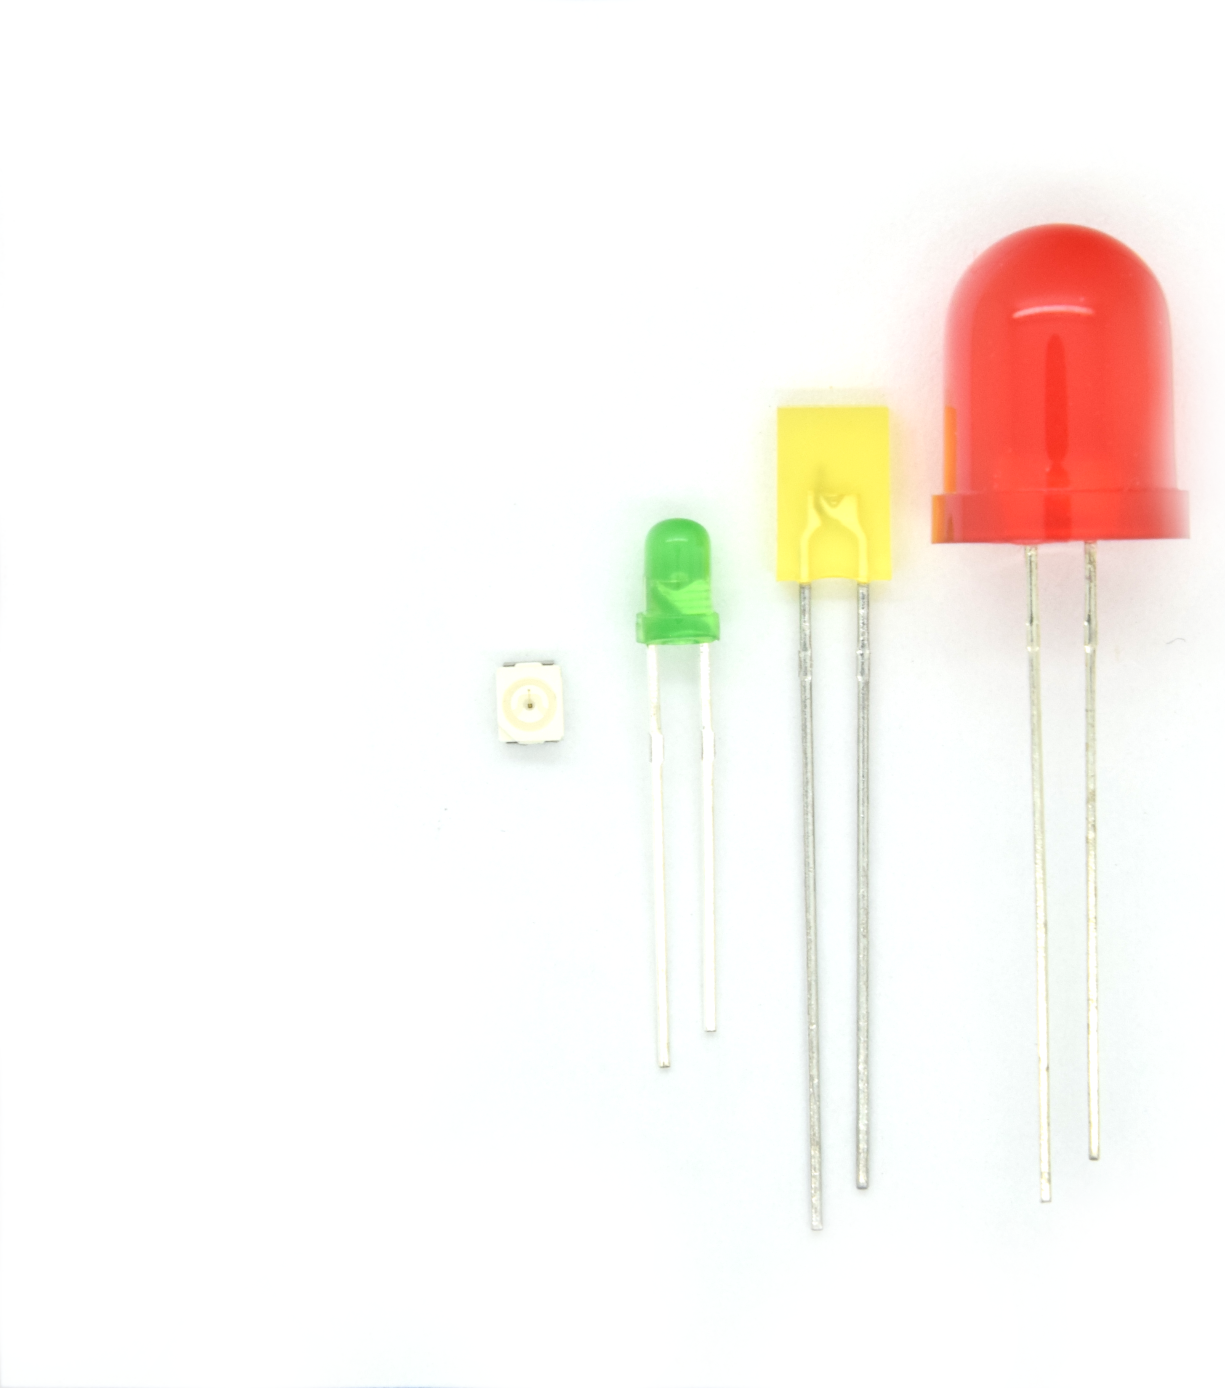
\includegraphics[width=0.85\textwidth]{foto/6}
    \caption{\scriptsize Diverse LED in verschiedenen Bauformen und Farben}
    \label{e_led}
\end{figure}

   \end{column}
\end{columns}

\end{frame}

\begin{frame}
\only<1>{
\begin{QQuestion}{EC501}{Eine in Sperrrichtung betriebene Diode zeichnet sich insbesondere aus durch~...}{eine hohe Induktivität.}
{eine hohe Kapazität.}
{eine geringe Impedanz.}
{einen hohen Widerstand.}
\end{QQuestion}

}
\only<2>{
\begin{QQuestion}{EC501}{Eine in Sperrrichtung betriebene Diode zeichnet sich insbesondere aus durch~...}{eine hohe Induktivität.}
{eine hohe Kapazität.}
{eine geringe Impedanz.}
{\textbf{\textcolor{DARCgreen}{einen hohen Widerstand.}}}
\end{QQuestion}

}
\end{frame}

\begin{frame}
\only<1>{
\begin{QQuestion}{EC502}{Wofür können Halbleiterdioden beispielsweise verwendet werden?}{zur Speicherung von Wechselströmen}
{zur Gleichrichtung von Wechselspannung}
{als Widerstand in Netzteilen}
{als Verstärker in Stromversorgungen}
\end{QQuestion}

}
\only<2>{
\begin{QQuestion}{EC502}{Wofür können Halbleiterdioden beispielsweise verwendet werden?}{zur Speicherung von Wechselströmen}
{\textbf{\textcolor{DARCgreen}{zur Gleichrichtung von Wechselspannung}}}
{als Widerstand in Netzteilen}
{als Verstärker in Stromversorgungen}
\end{QQuestion}

}
\end{frame}

\begin{frame}
\frametitle{Schwellenspannung}
\begin{columns}
    \begin{column}{0.48\textwidth}
    \begin{itemize}
  \item Damit eine Diode in Durchlassrichtung leitet, muss eine bestimmte Spannung -- die Schwellenspannung oder Durchlassspannung -- überschritten werden
  \item Je nach Basis des chemischen Elements ist die Schwellenspannung unterschiedlich hoch
  \end{itemize}

    \end{column}
   \begin{column}{0.48\textwidth}
       \begin{itemize}
  \item Germanium: \qty{0,2}{\volt}-\qty{0,4}{\volt}
  \item Silizium: \qty{0,6}{\volt}-\qty{0,8}{\volt}
  \item LED (Rot): \qty{1,6}{\volt}-\qty{2,2}{\volt}
  \item LED (Gelb, Grün): \qty{1,9}{\volt}-\qty{2,5}{\volt}
  \item LED (Blau, Weiß): \qty{2,7}{\volt}-\qty{3,5}{\volt}
  \end{itemize}

   \end{column}
\end{columns}

\end{frame}

\begin{frame}
\only<1>{
\begin{QQuestion}{EC503}{Welche typischen Schwellspannungen haben Germanium- und Siliziumdioden? Sie liegen bei~...}{Germanium zwischen \qtyrange{0,6}{0,8}{\V}, bei Silizium \qtyrange{1,4}{1,6}{\V}.}
{Germanium zwischen \qtyrange{0,6}{0,8}{\V}, bei Silizium zwischen \qtyrange{0,2}{0,4}{\V}.}
{Germanium zwischen \qtyrange{1,4}{1,6}{\V}, bei Silizium \qtyrange{0,6}{0,8}{\V}.}
{Germanium zwischen \qtyrange{0,2}{0,4}{\V}, bei Silizium zwischen \qtyrange{0,6}{0,8}{\V}.}
\end{QQuestion}

}
\only<2>{
\begin{QQuestion}{EC503}{Welche typischen Schwellspannungen haben Germanium- und Siliziumdioden? Sie liegen bei~...}{Germanium zwischen \qtyrange{0,6}{0,8}{\V}, bei Silizium \qtyrange{1,4}{1,6}{\V}.}
{Germanium zwischen \qtyrange{0,6}{0,8}{\V}, bei Silizium zwischen \qtyrange{0,2}{0,4}{\V}.}
{Germanium zwischen \qtyrange{1,4}{1,6}{\V}, bei Silizium \qtyrange{0,6}{0,8}{\V}.}
{\textbf{\textcolor{DARCgreen}{Germanium zwischen \qtyrange{0,2}{0,4}{\V}, bei Silizium zwischen \qtyrange{0,6}{0,8}{\V}.}}}
\end{QQuestion}

}
\end{frame}

\begin{frame}
\frametitle{Schottky-Diode}
\begin{itemize}
  \item Erlaubt eine hohe Schaltfrequenz
  \item Nur eine sehr niedrige Schwellenspannung von \qty{0,4}{\volt} bis unter \qty{0,1}{\volt} ist nötig
  \end{itemize}
\end{frame}

\begin{frame}
\only<1>{
\begin{QQuestion}{EC504}{Welches sind die Haupteigenschaften einer Schottkydiode?}{Sehr niedrige Durchlassspannung und sehr hohe Schaltfrequenz.}
{Sehr niedrige Durchlassspannung und sehr niedrige Schaltfrequenz.}
{Sehr hohe Durchlassspannung und sehr hohe Schaltfrequenz.}
{Sehr hohe Durchlassspannung und sehr niedrige Schaltfrequenz.}
\end{QQuestion}

}
\only<2>{
\begin{QQuestion}{EC504}{Welches sind die Haupteigenschaften einer Schottkydiode?}{\textbf{\textcolor{DARCgreen}{Sehr niedrige Durchlassspannung und sehr hohe Schaltfrequenz.}}}
{Sehr niedrige Durchlassspannung und sehr niedrige Schaltfrequenz.}
{Sehr hohe Durchlassspannung und sehr hohe Schaltfrequenz.}
{Sehr hohe Durchlassspannung und sehr niedrige Schaltfrequenz.}
\end{QQuestion}

}
\end{frame}

\begin{frame}
\frametitle{Kennlinien}
\end{frame}

\begin{frame}
\only<1>{
\begin{PQuestion}{EC506}{Welche Diode wird durch Kennlinie 2 charakterisiert?}{Germaniumdiode}
{Siliziumdiode}
{Schottkydiode}
{Leuchtdiode}
{\DARCimage{1.0\linewidth}{307include}}\end{PQuestion}

}
\only<2>{
\begin{PQuestion}{EC506}{Welche Diode wird durch Kennlinie 2 charakterisiert?}{\textbf{\textcolor{DARCgreen}{Germaniumdiode}}}
{Siliziumdiode}
{Schottkydiode}
{Leuchtdiode}
{\DARCimage{1.0\linewidth}{307include}}\end{PQuestion}

}
\end{frame}

\begin{frame}
\only<1>{
\begin{PQuestion}{EC507}{Welche Diode wird durch Kennlinie 3 charakterisiert?}{Schottkydiode}
{Leuchtdiode}
{Siliziumdiode}
{Germaniumdiode}
{\DARCimage{1.0\linewidth}{307include}}\end{PQuestion}

}
\only<2>{
\begin{PQuestion}{EC507}{Welche Diode wird durch Kennlinie 3 charakterisiert?}{Schottkydiode}
{Leuchtdiode}
{\textbf{\textcolor{DARCgreen}{Siliziumdiode}}}
{Germaniumdiode}
{\DARCimage{1.0\linewidth}{307include}}\end{PQuestion}

}
\end{frame}

\begin{frame}
\only<1>{
\begin{PQuestion}{EC508}{Welche Diode wird durch Kennlinie 4 charakterisiert?}{Leuchtdiode}
{Siliziumdiode}
{Schottkydiode}
{Germaniumdiode}
{\DARCimage{1.0\linewidth}{307include}}\end{PQuestion}

}
\only<2>{
\begin{PQuestion}{EC508}{Welche Diode wird durch Kennlinie 4 charakterisiert?}{\textbf{\textcolor{DARCgreen}{Leuchtdiode}}}
{Siliziumdiode}
{Schottkydiode}
{Germaniumdiode}
{\DARCimage{1.0\linewidth}{307include}}\end{PQuestion}

}
\end{frame}

\begin{frame}
\only<1>{
\begin{PQuestion}{EC505}{Welche Diode wird durch Kennlinie 1 charakterisiert?}{Germaniumdiode}
{Siliziumdiode}
{Schottkydiode}
{Leuchtdiode}
{\DARCimage{1.0\linewidth}{307include}}\end{PQuestion}

}
\only<2>{
\begin{PQuestion}{EC505}{Welche Diode wird durch Kennlinie 1 charakterisiert?}{Germaniumdiode}
{Siliziumdiode}
{\textbf{\textcolor{DARCgreen}{Schottkydiode}}}
{Leuchtdiode}
{\DARCimage{1.0\linewidth}{307include}}\end{PQuestion}

}
\end{frame}

\begin{frame}
\frametitle{Leitende Diode}
\begin{columns}
    \begin{column}{0.48\textwidth}
    \begin{itemize}
  \item Eine Diode leitet immer dann, wenn die Spannung an der Anode um die Schwellenspannung positiver ist als an der Kathode
  \item Gilt auch für negative Spannungen
  \item In der Prüfung kommen nur Siliziumdioden mit \qty{0,7}{\volt} Schwellenspannung vor
  \end{itemize}

    \end{column}
   \begin{column}{0.48\textwidth}
       
\begin{figure}
    \DARCimage{0.85\linewidth}{113include}
    \caption{\scriptsize Spannungen an einer leitenden Siliziumdiode}
    \label{e_leitende_siliziumdiode}
\end{figure}


   \end{column}
\end{columns}

\end{frame}

\begin{frame}
\only<1>{
\begin{QQuestion}{EC513}{Bei welcher Bedingung wird eine Siliziumdiode leitend?}{An der Anode liegen \qty{5,7}{\V}, an der Kathode \qty{5,0}{\V} an.}
{An der Anode liegen \qty{5,7}{\V}, an der Kathode \qty{6,4}{\V} an.}
{An der Anode liegen \qty{5,0}{\V}, an der Kathode \qty{5,1}{\V} an.}
{An der Anode liegen \qty{5,0}{\V}, an der Kathode \qty{5,7}{\V} an.}
\end{QQuestion}

}
\only<2>{
\begin{QQuestion}{EC513}{Bei welcher Bedingung wird eine Siliziumdiode leitend?}{\textbf{\textcolor{DARCgreen}{An der Anode liegen \qty{5,7}{\V}, an der Kathode \qty{5,0}{\V} an.}}}
{An der Anode liegen \qty{5,7}{\V}, an der Kathode \qty{6,4}{\V} an.}
{An der Anode liegen \qty{5,0}{\V}, an der Kathode \qty{5,1}{\V} an.}
{An der Anode liegen \qty{5,0}{\V}, an der Kathode \qty{5,7}{\V} an.}
\end{QQuestion}

}
\end{frame}

\begin{frame}
\only<1>{
\begin{question2x2}{EC510}{Die Auswahlantworten enthalten Siliziumdioden mit unterschiedlichen Arbeitspunkten. Bei welcher Antwort befindet sich die Diode in leitendem Zustand?}{\DARCimage{1.0\linewidth}{110include}}
{\DARCimage{1.0\linewidth}{109include}}
{\DARCimage{1.0\linewidth}{111include}}
{\DARCimage{1.0\linewidth}{112include}}
\end{question2x2}

}
\only<2>{
\begin{question2x2}{EC510}{Die Auswahlantworten enthalten Siliziumdioden mit unterschiedlichen Arbeitspunkten. Bei welcher Antwort befindet sich die Diode in leitendem Zustand?}{\DARCimage{1.0\linewidth}{110include}}
{\textbf{\textcolor{DARCgreen}{\DARCimage{1.0\linewidth}{109include}}}}
{\DARCimage{1.0\linewidth}{111include}}
{\DARCimage{1.0\linewidth}{112include}}
\end{question2x2}

}
\end{frame}

\begin{frame}
\only<1>{
\begin{question2x2}{EC509}{Die Auswahlantworten enthalten Siliziumdioden mit unterschiedlichen Arbeitspunkten. Bei welcher Antwort befindet sich die Diode in leitendem Zustand?}{\DARCimage{1.0\linewidth}{116include}}
{\DARCimage{1.0\linewidth}{114include}}
{\DARCimage{1.0\linewidth}{115include}}
{\DARCimage{1.0\linewidth}{113include}}
\end{question2x2}

}
\only<2>{
\begin{question2x2}{EC509}{Die Auswahlantworten enthalten Siliziumdioden mit unterschiedlichen Arbeitspunkten. Bei welcher Antwort befindet sich die Diode in leitendem Zustand?}{\DARCimage{1.0\linewidth}{116include}}
{\DARCimage{1.0\linewidth}{114include}}
{\DARCimage{1.0\linewidth}{115include}}
{\textbf{\textcolor{DARCgreen}{\DARCimage{1.0\linewidth}{113include}}}}
\end{question2x2}

}
\end{frame}

\begin{frame}
\only<1>{
\begin{question2x2}{EC511}{Die Auswahlantworten enthalten Siliziumdioden mit unterschiedlichen Arbeitspunkten. Bei welcher Antwort befindet sich die Diode in leitendem Zustand?}{\DARCimage{1.0\linewidth}{118include}}
{\DARCimage{1.0\linewidth}{117include}}
{\DARCimage{1.0\linewidth}{119include}}
{\DARCimage{1.0\linewidth}{120include}}
\end{question2x2}

}
\only<2>{
\begin{question2x2}{EC511}{Die Auswahlantworten enthalten Siliziumdioden mit unterschiedlichen Arbeitspunkten. Bei welcher Antwort befindet sich die Diode in leitendem Zustand?}{\DARCimage{1.0\linewidth}{118include}}
{\textbf{\textcolor{DARCgreen}{\DARCimage{1.0\linewidth}{117include}}}}
{\DARCimage{1.0\linewidth}{119include}}
{\DARCimage{1.0\linewidth}{120include}}
\end{question2x2}

}
\end{frame}

\begin{frame}
\only<1>{
\begin{question2x2}{EC512}{Die Auswahlantworten enthalten Siliziumdioden mit unterschiedlichen Arbeitspunkten. Bei welcher Antwort befindet sich die Diode in leitendem Zustand?}{\DARCimage{1.0\linewidth}{121include}}
{\DARCimage{1.0\linewidth}{122include}}
{\DARCimage{1.0\linewidth}{123include}}
{\DARCimage{1.0\linewidth}{124include}}
\end{question2x2}

}
\only<2>{
\begin{question2x2}{EC512}{Die Auswahlantworten enthalten Siliziumdioden mit unterschiedlichen Arbeitspunkten. Bei welcher Antwort befindet sich die Diode in leitendem Zustand?}{\textbf{\textcolor{DARCgreen}{\DARCimage{1.0\linewidth}{121include}}}}
{\DARCimage{1.0\linewidth}{122include}}
{\DARCimage{1.0\linewidth}{123include}}
{\DARCimage{1.0\linewidth}{124include}}
\end{question2x2}

}
\end{frame}

\begin{frame}
\frametitle{LED Anwendung }
\begin{columns}
    \begin{column}{0.48\textwidth}
    \begin{itemize}
  \item Eine LED dient als Leuchtanzeige
  \end{itemize}

    \end{column}
   \begin{column}{0.48\textwidth}
       
\begin{figure}
    \DARCimage{0.85\linewidth}{324include}
    \caption{\scriptsize LED mit Vorwiderstand}
    \label{e_led_schaltung}
\end{figure}


   \end{column}
\end{columns}

\end{frame}

\begin{frame}
\only<1>{
\begin{PQuestion}{EC514}{Wozu dient die folgende Schaltung?}{Spannungserhöhung}
{Leuchtanzeige}
{Leistungsüberwachung}
{Stromgewinnung}
{\DARCimage{0.75\linewidth}{324include}}\end{PQuestion}

}
\only<2>{
\begin{PQuestion}{EC514}{Wozu dient die folgende Schaltung?}{Spannungserhöhung}
{\textbf{\textcolor{DARCgreen}{Leuchtanzeige}}}
{Leistungsüberwachung}
{Stromgewinnung}
{\DARCimage{0.75\linewidth}{324include}}\end{PQuestion}

}
\end{frame}

\begin{frame}
\frametitle{Vorwiderstand}
\begin{columns}
    \begin{column}{0.48\textwidth}
    \begin{itemize}
  \item Da die LED selbst kaum einen Widerstand hat, würde sie bei einem direkten Anschluss an eine Spannungsquelle wie ein Kurzschluss wirken
  \item Mit einem Vorwiderstand wird der Durchlassstrom begrenzt
  \end{itemize}

    \end{column}
   \begin{column}{0.48\textwidth}
       
\begin{figure}
    \DARCimage{0.85\linewidth}{324include}
    \caption{\scriptsize LED mit Vorwiderstand}
    \label{e_led_schaltung}
\end{figure}


   \end{column}
\end{columns}

\end{frame}

\begin{frame}\begin{itemize}
  \item Berechnung: $R = \dfrac{U_q -- U_{LED}}{I_D}$
  \item $U_q$: Spannungsquelle
  \item $U_{LED}$: Schwellenspannung LED
  \item $I_D$: Durchlassstrom
  \end{itemize}
\end{frame}

\begin{frame}
\only<1>{
\begin{QQuestion}{EC515}{Eine Leuchtdiode mit einer Durchlassspannung von \qty{1,4}{\V} und einem Durchlassstrom von \qty{20}{\mA} soll an eine Spannungsquelle von \qty{5,0}{\V} angeschlossen werden. Berechnen Sie den Vorwiderstand. Die Größe des benötigten Vorwiderstandes beträgt~...}{\qty{180}{\ohm}.}
{\qty{250}{\ohm}.}
{\qty{70}{\ohm}.}
{\qty{320}{\ohm}.}
\end{QQuestion}

}
\only<2>{
\begin{QQuestion}{EC515}{Eine Leuchtdiode mit einer Durchlassspannung von \qty{1,4}{\V} und einem Durchlassstrom von \qty{20}{\mA} soll an eine Spannungsquelle von \qty{5,0}{\V} angeschlossen werden. Berechnen Sie den Vorwiderstand. Die Größe des benötigten Vorwiderstandes beträgt~...}{\textbf{\textcolor{DARCgreen}{\qty{180}{\ohm}.}}}
{\qty{250}{\ohm}.}
{\qty{70}{\ohm}.}
{\qty{320}{\ohm}.}
\end{QQuestion}

}
\end{frame}

\begin{frame}
\only<1>{
\begin{PQuestion}{EC516}{Folgende Schaltung einer Leuchtdiode wird an einer Betriebsspannung von \qty{5,5}{\V} betrieben. Der Strom durch die Leuchtdiode soll \qty{25}{\mA} betragen, wobei die Durchlassspannung \qty{1,75}{\V} beträgt. Der notwendige Vorwiderstand muss folgende Werte haben:}{\qty{150}{\ohm}/\qty{0,1}{\W}}
{\qty{150}{\ohm}/\qty{0,06}{\W}}
{\qty{70}{\ohm}/\qty{0,1}{\W}}
{\qty{70}{\ohm}/\qty{0,06}{\W}}
{\DARCimage{0.75\linewidth}{324include}}\end{PQuestion}

}
\only<2>{
\begin{PQuestion}{EC516}{Folgende Schaltung einer Leuchtdiode wird an einer Betriebsspannung von \qty{5,5}{\V} betrieben. Der Strom durch die Leuchtdiode soll \qty{25}{\mA} betragen, wobei die Durchlassspannung \qty{1,75}{\V} beträgt. Der notwendige Vorwiderstand muss folgende Werte haben:}{\textbf{\textcolor{DARCgreen}{\qty{150}{\ohm}/\qty{0,1}{\W}}}}
{\qty{150}{\ohm}/\qty{0,06}{\W}}
{\qty{70}{\ohm}/\qty{0,1}{\W}}
{\qty{70}{\ohm}/\qty{0,06}{\W}}
{\DARCimage{0.75\linewidth}{324include}}\end{PQuestion}

}
\end{frame}

\begin{frame}
\frametitle{Z-Diode}
\begin{columns}
    \begin{column}{0.48\textwidth}
    \begin{itemize}
  \item Normalerweise liegt die maximale Sperrspannung einer Diode bei ca. \qty{1000}{\volt}
  \item Bei Z-Dioden erfolgt ein Spannungsdurchbruch je nach Bauart zwischen \qty{3}{\volt} und \qty{100}{\volt}
  \item Dienen zur Spannungsstabilisierung
  \end{itemize}

    \end{column}
   \begin{column}{0.48\textwidth}
       
\begin{figure}
    \DARCimage{0.85\linewidth}{560include}
    \caption{\scriptsize Schaltzeichen Z-Diode}
    \label{_e_z_diode}
\end{figure}


   \end{column}
\end{columns}

\end{frame}

\begin{frame}
\frametitle{Polung}
\begin{columns}
    \begin{column}{0.48\textwidth}
    \begin{itemize}
  \item Z-Dioden werden mit Vorwiderstand in Sperrrichtung betrieben
  \end{itemize}

    \end{column}
   \begin{column}{0.48\textwidth}
       
\begin{figure}
    \DARCimage{0.85\linewidth}{549include}
    \caption{\scriptsize Z-Diode korrekt in Sperrichtung eingesetzt}
    \label{e_z_diode_polung}
\end{figure}


   \end{column}
\end{columns}

\end{frame}

\begin{frame}
\only<1>{
\begin{PQuestion}{EC517}{Welches Bauteil wird durch das Schaltzeichen symbolisiert?}{Z-Diode}
{Leuchtdiode}
{Kapazitätsdiode}
{Freilaufdiode}
{\DARCimage{0.5\linewidth}{560include}}\end{PQuestion}

}
\only<2>{
\begin{PQuestion}{EC517}{Welches Bauteil wird durch das Schaltzeichen symbolisiert?}{\textbf{\textcolor{DARCgreen}{Z-Diode}}}
{Leuchtdiode}
{Kapazitätsdiode}
{Freilaufdiode}
{\DARCimage{0.5\linewidth}{560include}}\end{PQuestion}

}
\end{frame}

\begin{frame}
\only<1>{
\begin{QQuestion}{EC518}{Für welchen Zweck werden Z-Dioden primär eingesetzt?}{Zur Stromstabilisierung}
{Zur Spannungsstabilisierung}
{Zur Zweiwegstabilisierung}
{Zur Leistungsstabilisierung}
\end{QQuestion}

}
\only<2>{
\begin{QQuestion}{EC518}{Für welchen Zweck werden Z-Dioden primär eingesetzt?}{Zur Stromstabilisierung}
{\textbf{\textcolor{DARCgreen}{Zur Spannungsstabilisierung}}}
{Zur Zweiwegstabilisierung}
{Zur Leistungsstabilisierung}
\end{QQuestion}

}
\end{frame}

\begin{frame}
\only<1>{
\begin{PQuestion}{EC519}{Wozu dient folgende Schaltung?}{Spannungsstabilisierung}
{Spannungserhöhung}
{Leuchtanzeige}
{Stromgewinnung}
{\DARCimage{1.0\linewidth}{549include}}\end{PQuestion}

}
\only<2>{
\begin{PQuestion}{EC519}{Wozu dient folgende Schaltung?}{\textbf{\textcolor{DARCgreen}{Spannungsstabilisierung}}}
{Spannungserhöhung}
{Leuchtanzeige}
{Stromgewinnung}
{\DARCimage{1.0\linewidth}{549include}}\end{PQuestion}

}
\end{frame}

\begin{frame}
\only<1>{
\begin{question2x2}{EC520}{In welcher der folgenden Schaltungen ist die Z-Diode zur Spannungsstabilisierung richtig eingesetzt?}{\DARCimage{1.0\linewidth}{317include}}
{\DARCimage{1.0\linewidth}{318include}}
{\DARCimage{1.0\linewidth}{319include}}
{\DARCimage{1.0\linewidth}{320include}}
\end{question2x2}

}
\only<2>{
\begin{question2x2}{EC520}{In welcher der folgenden Schaltungen ist die Z-Diode zur Spannungsstabilisierung richtig eingesetzt?}{\textbf{\textcolor{DARCgreen}{\DARCimage{1.0\linewidth}{317include}}}}
{\DARCimage{1.0\linewidth}{318include}}
{\DARCimage{1.0\linewidth}{319include}}
{\DARCimage{1.0\linewidth}{320include}}
\end{question2x2}

}
\end{frame}

\begin{frame}
\frametitle{Vorwiderstand}
\begin{columns}
    \begin{column}{0.48\textwidth}
    \begin{itemize}
  \item $U_Z$ ist die Spannung, auf die die Z-Diode stabiliert
  \item $U_V = U_1 -- U_Z = 13,8\,V -- 5\,V = 8,8\,V$
  \item $R_V = \frac{U_V}{I} = \frac{8,8\,V}{30\,mA} \approx 293\,\Omega$
  \end{itemize}

    \end{column}
   \begin{column}{0.48\textwidth}
       
\begin{figure}
    \DARCimage{0.85\linewidth}{753include}
    \caption{\scriptsize Z-Diode zur Spannungsstabilisierung}
    \label{e_z_diode_spannungsstabilisierung}
\end{figure}


   \end{column}
\end{columns}

\end{frame}

\begin{frame}
\only<1>{
\begin{PQuestion}{EC521}{Eine unbelastete Z-Diode soll eine \qty{13,8}{\V} Betriebsspannung auf \qty{5}{\V} stabilisieren. Dabei soll ein Strom von \qty{30}{\mA} durch die Z-Diode fließen. Der Ausgang der Schaltung soll nicht belastet werden. Berechnen Sie den Wert des Vorwiderstands.}{ca. \qty{167}{\ohm}}
{ca. \qty{3,41}{\milli\ohm}}
{ca. \qty{460}{\ohm}}
{ca. \qty{293}{\ohm}}
{\DARCimage{1.0\linewidth}{753include}}\end{PQuestion}

}
\only<2>{
\begin{PQuestion}{EC521}{Eine unbelastete Z-Diode soll eine \qty{13,8}{\V} Betriebsspannung auf \qty{5}{\V} stabilisieren. Dabei soll ein Strom von \qty{30}{\mA} durch die Z-Diode fließen. Der Ausgang der Schaltung soll nicht belastet werden. Berechnen Sie den Wert des Vorwiderstands.}{ca. \qty{167}{\ohm}}
{ca. \qty{3,41}{\milli\ohm}}
{ca. \qty{460}{\ohm}}
{\textbf{\textcolor{DARCgreen}{ca. \qty{293}{\ohm}}}}
{\DARCimage{1.0\linewidth}{753include}}\end{PQuestion}

}
\end{frame}

\begin{frame}
\only<1>{
\begin{PQuestion}{EC522}{Folgende Schaltung einer Stabilisierungsschaltung mit Z-Diode ist gegeben. Der Strom durch die Z-Diode soll \qty{25}{\mA} betragen und der Laststrom ist \qty{20}{\mA}. Der Wert des notwendigen Vorwiderstandes beträgt~...}{ca. \qty{364}{\ohm}.}
{ca. \qty{202}{\ohm}.}
{ca. \qty{188}{\ohm}.}
{ca. \qty{235}{\ohm}.}
{\DARCimage{1.0\linewidth}{758include}}\end{PQuestion}

}
\only<2>{
\begin{PQuestion}{EC522}{Folgende Schaltung einer Stabilisierungsschaltung mit Z-Diode ist gegeben. Der Strom durch die Z-Diode soll \qty{25}{\mA} betragen und der Laststrom ist \qty{20}{\mA}. Der Wert des notwendigen Vorwiderstandes beträgt~...}{ca. \qty{364}{\ohm}.}
{\textbf{\textcolor{DARCgreen}{ca. \qty{202}{\ohm}.}}}
{ca. \qty{188}{\ohm}.}
{ca. \qty{235}{\ohm}.}
{\DARCimage{1.0\linewidth}{758include}}\end{PQuestion}

}

\end{frame}%ENDCONTENT


\section{Diode II}
\label{section:diode_2}
\begin{frame}%STARTCONTENT

\only<1>{
\begin{QQuestion}{AC401}{Ein in Durchlassrichtung betriebener PN-Übergang ermöglicht~...}{den Elektronenfluss von P nach N.}
{die Halbierung des Stromflusses.}
{keinen Stromfluss.}
{den Elektronenfluss von N nach P.}
\end{QQuestion}

}
\only<2>{
\begin{QQuestion}{AC401}{Ein in Durchlassrichtung betriebener PN-Übergang ermöglicht~...}{den Elektronenfluss von P nach N.}
{die Halbierung des Stromflusses.}
{keinen Stromfluss.}
{\textbf{\textcolor{DARCgreen}{den Elektronenfluss von N nach P.}}}
\end{QQuestion}

}
\end{frame}

\begin{frame}
\only<1>{
\begin{QQuestion}{AC403}{Wie verhält sich die Durchlassspannung einer Diode in Abhängigkeit von der Temperatur?}{Die Spannung ist unabhängig von der Temperatur.}
{Die Spannung sinkt bei steigender Temperatur.}
{Die Spannung oszilliert mit steigender Temperatur.}
{Die Spannung steigt bei steigender Temperatur.}
\end{QQuestion}

}
\only<2>{
\begin{QQuestion}{AC403}{Wie verhält sich die Durchlassspannung einer Diode in Abhängigkeit von der Temperatur?}{Die Spannung ist unabhängig von der Temperatur.}
{\textbf{\textcolor{DARCgreen}{Die Spannung sinkt bei steigender Temperatur.}}}
{Die Spannung oszilliert mit steigender Temperatur.}
{Die Spannung steigt bei steigender Temperatur.}
\end{QQuestion}

}
\end{frame}

\begin{frame}
\only<1>{
\begin{QQuestion}{AC404}{Wie verhält sich die Kapazität einer Kapazitätsdiode (Varicap)?}{Sie nimmt mit abnehmender Sperrspannung zu.}
{Sie nimmt mit abnehmendem Durchlassstrom zu.}
{Sie nimmt mit zunehmender Sperrspannung zu.}
{Sie nimmt mit zunehmendem Durchlassstrom zu.}
\end{QQuestion}

}
\only<2>{
\begin{QQuestion}{AC404}{Wie verhält sich die Kapazität einer Kapazitätsdiode (Varicap)?}{\textbf{\textcolor{DARCgreen}{Sie nimmt mit abnehmender Sperrspannung zu.}}}
{Sie nimmt mit abnehmendem Durchlassstrom zu.}
{Sie nimmt mit zunehmender Sperrspannung zu.}
{Sie nimmt mit zunehmendem Durchlassstrom zu.}
\end{QQuestion}

}
\end{frame}

\begin{frame}
\only<1>{
\begin{PQuestion}{AC405}{Das folgende Signal wird als $U_1$ an den Eingang der Schaltung mit Siliziumdioden gelegt. Wie sieht das zugehörige Ausgangssignal $U_2$ aus?}{\DARCimage{1.0\linewidth}{17include}}
{\DARCimage{1.0\linewidth}{15include}}
{\DARCimage{1.0\linewidth}{16include}}
{\DARCimage{1.0\linewidth}{14include}}
{\DARCimage{1.0\linewidth}{13include}}\end{PQuestion}

}
\only<2>{
\begin{PQuestion}{AC405}{Das folgende Signal wird als $U_1$ an den Eingang der Schaltung mit Siliziumdioden gelegt. Wie sieht das zugehörige Ausgangssignal $U_2$ aus?}{\DARCimage{1.0\linewidth}{17include}}
{\DARCimage{1.0\linewidth}{15include}}
{\DARCimage{1.0\linewidth}{16include}}
{\textbf{\textcolor{DARCgreen}{\DARCimage{1.0\linewidth}{14include}}}}
{\DARCimage{1.0\linewidth}{13include}}\end{PQuestion}

}
\end{frame}

\begin{frame}
\only<1>{
\begin{PQuestion}{AC406}{Das folgende Signal wird als $U_1$ an den Eingang der Schaltung mit Germaniumdioden gelegt. Wie sieht das zugehörige Ausgangssignal $U_2$ aus?}{\DARCimage{1.0\linewidth}{17include}}
{\DARCimage{1.0\linewidth}{15include}}
{\DARCimage{1.0\linewidth}{16include}}
{\DARCimage{1.0\linewidth}{14include}}
{\DARCimage{1.0\linewidth}{13include}}\end{PQuestion}

}
\only<2>{
\begin{PQuestion}{AC406}{Das folgende Signal wird als $U_1$ an den Eingang der Schaltung mit Germaniumdioden gelegt. Wie sieht das zugehörige Ausgangssignal $U_2$ aus?}{\textbf{\textcolor{DARCgreen}{\DARCimage{1.0\linewidth}{17include}}}}
{\DARCimage{1.0\linewidth}{15include}}
{\DARCimage{1.0\linewidth}{16include}}
{\DARCimage{1.0\linewidth}{14include}}
{\DARCimage{1.0\linewidth}{13include}}\end{PQuestion}

}
\end{frame}

\begin{frame}
\only<1>{
\begin{QQuestion}{AC407}{Welches Bauteil kann durch Lichteinfall elektrischen Strom erzeugen?}{Blindwiderstand}
{Fotowiderstand}
{Kapazitätsdiode}
{Fotodiode}
\end{QQuestion}

}
\only<2>{
\begin{QQuestion}{AC407}{Welches Bauteil kann durch Lichteinfall elektrischen Strom erzeugen?}{Blindwiderstand}
{Fotowiderstand}
{Kapazitätsdiode}
{\textbf{\textcolor{DARCgreen}{Fotodiode}}}
\end{QQuestion}

}
\end{frame}

\begin{frame}
\only<1>{
\begin{QQuestion}{AC408}{Die Hauptfunktion eines Optokopplers ist~...}{die galvanische Entkopplung zweier Stromkreise durch Licht.}
{die Erzeugung von hochfrequentem Wechselstrom durch Licht.}
{die Signalanzeige durch Licht.}
{die Erzeugung von Gleichstrom durch Licht.}
\end{QQuestion}

}
\only<2>{
\begin{QQuestion}{AC408}{Die Hauptfunktion eines Optokopplers ist~...}{\textbf{\textcolor{DARCgreen}{die galvanische Entkopplung zweier Stromkreise durch Licht.}}}
{die Erzeugung von hochfrequentem Wechselstrom durch Licht.}
{die Signalanzeige durch Licht.}
{die Erzeugung von Gleichstrom durch Licht.}
\end{QQuestion}

}
\end{frame}%ENDCONTENT


\section{Transistor I}
\label{section:transistor_1}
\begin{frame}%STARTCONTENT

\frametitle{Von der Diode zum Transistor}
\begin{columns}
    \begin{column}{0.48\textwidth}
    Die Funktion kann man sich so vorstellen:

\begin{itemize}
  \item Mittels eines Steuerkanals wird der Durchfluss eines Wehrs geregelt
  \item Fließt kein Wasser im Steuerkanal ist das Wehr geschlossen
  \end{itemize}

    \end{column}
   \begin{column}{0.48\textwidth}
       
\begin{figure}
    \DARCimage{0.85\linewidth}{835include}
    \caption{\scriptsize Steuerkanal schließt Wehr komplett}
    \label{e_transistor_wehr_geschlossen}
\end{figure}


   \end{column}
\end{columns}

\end{frame}

\begin{frame}
\frametitle{Von der Diode zum Transistor}
\begin{columns}
    \begin{column}{0.48\textwidth}
    Die Funktion kann man sich so vorstellen:

\begin{itemize}
  \item Fließt etwas Wasser im Steuerkanal, öffnet das Wehr zur Hälfte
  \end{itemize}

    \end{column}
   \begin{column}{0.48\textwidth}
       
\begin{figure}
    \DARCimage{0.85\linewidth}{837include}
    \caption{\scriptsize Steuerkanal öffnet Wehr halb}
    \label{e_transistor_wehr_halb_offen}
\end{figure}


   \end{column}
\end{columns}

\end{frame}

\begin{frame}
\frametitle{Von der Diode zum Transistor}
\begin{columns}
    \begin{column}{0.48\textwidth}
    Die Funktion kann man sich so vorstellen:

\begin{itemize}
  \item Fließt mehr Wasser im Steuerkanal, ist das Wehr ganz geöffnet
  \end{itemize}

    \end{column}
   \begin{column}{0.48\textwidth}
       
\begin{figure}
    \DARCimage{0.85\linewidth}{836include}
    \caption{\scriptsize Steuerkanal öffnet Wehr komplett}
    \label{e_transistor_wehr_geoeffnet}
\end{figure}


   \end{column}
\end{columns}

\end{frame}

\begin{frame}
\only<1>{
\begin{QQuestion}{EC602}{Ein Transistor ist~...}{ein Nichtleiterbauelement.}
{ein Laserbauelement.}
{ein Halbleiterbauelement.}
{ein Kaltleiterbauelement.}
\end{QQuestion}

}
\only<2>{
\begin{QQuestion}{EC602}{Ein Transistor ist~...}{ein Nichtleiterbauelement.}
{ein Laserbauelement.}
{\textbf{\textcolor{DARCgreen}{ein Halbleiterbauelement.}}}
{ein Kaltleiterbauelement.}
\end{QQuestion}

}
\end{frame}

\begin{frame}
\only<1>{
\begin{QQuestion}{EC608}{Wie lauten die Bezeichnungen der Anschlüsse eines bipolaren Transistors?}{Emitter, Basis, Kollektor}
{Emitter, Drain, Source}
{Gate, Source, Kollektor}
{Drain, Gate, Source}
\end{QQuestion}

}
\only<2>{
\begin{QQuestion}{EC608}{Wie lauten die Bezeichnungen der Anschlüsse eines bipolaren Transistors?}{\textbf{\textcolor{DARCgreen}{Emitter, Basis, Kollektor}}}
{Emitter, Drain, Source}
{Gate, Source, Kollektor}
{Drain, Gate, Source}
\end{QQuestion}

}
\end{frame}

\begin{frame}
\frametitle{Bipolarer Transistor und Schaltbild}
\begin{columns}
    \begin{column}{0.48\textwidth}
    Merksatz für PNP $\rightarrow$ Pfeil Nach Platte


    \end{column}
   \begin{column}{0.48\textwidth}
       
\begin{figure}
    \DARCimage{0.85\linewidth}{374include}
    \caption{\scriptsize Schaltbild NPN-Transistor}
    \label{e_schaltbild_npn_transistor}
\end{figure}


\begin{figure}
    \DARCimage{0.85\linewidth}{375include}
    \caption{\scriptsize Schaltbild PNP-Transistor}
    \label{e_schaltbild_pnp_transistor}
\end{figure}


   \end{column}
\end{columns}

\end{frame}

\begin{frame}
\only<1>{
\begin{PQuestion}{EC607}{Bei diesem Bauelement handelt es sich um einen }{PNP-Transistor.}
{NPN-Transistor.}
{P-Kanal-FET.}
{N-Kanal-FET.}
{\DARCimage{0.25\linewidth}{375include}}\end{PQuestion}

}
\only<2>{
\begin{PQuestion}{EC607}{Bei diesem Bauelement handelt es sich um einen }{\textbf{\textcolor{DARCgreen}{PNP-Transistor.}}}
{NPN-Transistor.}
{P-Kanal-FET.}
{N-Kanal-FET.}
{\DARCimage{0.25\linewidth}{375include}}\end{PQuestion}

}
\end{frame}

\begin{frame}
\only<1>{
\begin{PQuestion}{EC606}{Bei diesem Bauelement handelt es sich um einen }{PNP-Transistor.}
{NPN-Transistor.}
{N-Kanal-FET.}
{P-Kanal-FET.}
{\DARCimage{0.25\linewidth}{374include}}\end{PQuestion}

}
\only<2>{
\begin{PQuestion}{EC606}{Bei diesem Bauelement handelt es sich um einen }{PNP-Transistor.}
{\textbf{\textcolor{DARCgreen}{NPN-Transistor.}}}
{N-Kanal-FET.}
{P-Kanal-FET.}
{\DARCimage{0.25\linewidth}{374include}}\end{PQuestion}

}
\end{frame}

\begin{frame}
\only<1>{
\begin{question2x2}{EC605}{Welches Schaltzeichen stellt einen bipolaren Transistor dar?}{\DARCimage{1.0\linewidth}{433include}}
{\DARCimage{1.0\linewidth}{381include}}
{\DARCimage{1.0\linewidth}{374include}}
{\DARCimage{1.0\linewidth}{432include}}
\end{question2x2}

}
\only<2>{
\begin{question2x2}{EC605}{Welches Schaltzeichen stellt einen bipolaren Transistor dar?}{\DARCimage{1.0\linewidth}{433include}}
{\DARCimage{1.0\linewidth}{381include}}
{\textbf{\textcolor{DARCgreen}{\DARCimage{1.0\linewidth}{374include}}}}
{\DARCimage{1.0\linewidth}{432include}}
\end{question2x2}

}
\end{frame}

\begin{frame}
\only<1>{
\begin{PQuestion}{EC609}{Wie bezeichnet man die Anschlüsse des abgebildeten Transistors?}{1~=~Kollektor, 2~=~Basis, 3~=~Emitter}
{1~=~Emitter, 2~=~Basis, 3~=~Kollektor}
{1~=~Kollektor, 2~=~Emitter, 3~=~Basis}
{1~=~Basis, 2~=~Emitter, 3~=~Kollektor}
{\DARCimage{0.25\linewidth}{502include}}\end{PQuestion}

}
\only<2>{
\begin{PQuestion}{EC609}{Wie bezeichnet man die Anschlüsse des abgebildeten Transistors?}{\textbf{\textcolor{DARCgreen}{1~=~Kollektor, 2~=~Basis, 3~=~Emitter}}}
{1~=~Emitter, 2~=~Basis, 3~=~Kollektor}
{1~=~Kollektor, 2~=~Emitter, 3~=~Basis}
{1~=~Basis, 2~=~Emitter, 3~=~Kollektor}
{\DARCimage{0.25\linewidth}{502include}}\end{PQuestion}

}
\end{frame}

\begin{frame}
\frametitle{Schalter oder Verstärker?}
\begin{itemize}
  \item Die Ansteuerung kann so eingestellt werden, dass der Transistor sperrt oder voll durchsteuert, dann spricht man von einem Schalttransistor.
  \item Die Ansteuerung kann so eingestellt werden, dass der Transistor stufenlos gesteuert wird, dann spricht man von einem Verstärker.
  \end{itemize}
\end{frame}

\begin{frame}
\only<1>{
\begin{QQuestion}{EC601}{Welches Bauteil kann als Schalter, Verstärker oder Widerstand eingesetzt werden?}{Diode}
{Transformator}
{Kondensator}
{Transistor}
\end{QQuestion}

}
\only<2>{
\begin{QQuestion}{EC601}{Welches Bauteil kann als Schalter, Verstärker oder Widerstand eingesetzt werden?}{Diode}
{Transformator}
{Kondensator}
{\textbf{\textcolor{DARCgreen}{Transistor}}}
\end{QQuestion}

}
\end{frame}

\begin{frame}
\only<1>{
\begin{QQuestion}{EC603}{Was versteht man unter Stromverstärkung beim Transistor?}{Mit einem geringen Kollektorstrom wird ein großer Emitterstrom gesteuert.}
{Mit einem geringen Emitterstrom wird ein großer Kollektorstrom gesteuert.}
{Mit einem geringen Emitterstrom wird ein großer Basisstrom gesteuert.}
{Mit einem geringen Basisstrom wird ein großer Kollektorstrom gesteuert.}
\end{QQuestion}

}
\only<2>{
\begin{QQuestion}{EC603}{Was versteht man unter Stromverstärkung beim Transistor?}{Mit einem geringen Kollektorstrom wird ein großer Emitterstrom gesteuert.}
{Mit einem geringen Emitterstrom wird ein großer Kollektorstrom gesteuert.}
{Mit einem geringen Emitterstrom wird ein großer Basisstrom gesteuert.}
{\textbf{\textcolor{DARCgreen}{Mit einem geringen Basisstrom wird ein großer Kollektorstrom gesteuert.}}}
\end{QQuestion}

}
\end{frame}

\begin{frame}
\frametitle{Ansteuerspannung und deren Polarität}
Je Art des bipolaren Transistor hat man verschiedene Polaritäten.

\begin{itemize}
  \item Bei einem NPN-Transistor benötigt man zum Durchschalten eine positive Steuerspannung.
  \item Bei einem PNP-Transistor benötigt man zum Durchschalten eine negative Steuerspannung.
  \end{itemize}
Die Steuerspannung liegt wie bei einer Siliziumdiode bei etwa \qty{0,6}{\volt}.

\end{frame}

\begin{frame}
\only<1>{
\begin{PQuestion}{EC610}{Wie groß muss die Spannung $U_{BE}$ in etwa sein, sodass sich der Transistor im leitenden Betriebszustand befindet?}{\qty{-0,6}{\V}}
{\qty{0,6}{\V}}
{\qty{0,6}{\V} oder \qty{-0,6}{\V}}
{\qty{0}{\V}}
{\DARCimage{0.5\linewidth}{559include}}\end{PQuestion}

}
\only<2>{
\begin{PQuestion}{EC610}{Wie groß muss die Spannung $U_{BE}$ in etwa sein, sodass sich der Transistor im leitenden Betriebszustand befindet?}{\qty{-0,6}{\V}}
{\textbf{\textcolor{DARCgreen}{\qty{0,6}{\V}}}}
{\qty{0,6}{\V} oder \qty{-0,6}{\V}}
{\qty{0}{\V}}
{\DARCimage{0.5\linewidth}{559include}}\end{PQuestion}

}
\end{frame}

\begin{frame}Da neben dem Kollektorstrom auch der Basisstrom durch den Transistor fließt, fließt durch den Emitteranschluss der größte Strom.

\end{frame}

\begin{frame}
\only<1>{
\begin{QQuestion}{EC611}{Durch welchen Transistoranschluss fliesst im leitenden Zustand der größte Strom?}{Gehäuse}
{Kollektor}
{Basis}
{Emitter}
\end{QQuestion}

}
\only<2>{
\begin{QQuestion}{EC611}{Durch welchen Transistoranschluss fliesst im leitenden Zustand der größte Strom?}{Gehäuse}
{Kollektor}
{Basis}
{\textbf{\textcolor{DARCgreen}{Emitter}}}
\end{QQuestion}

}
\end{frame}

\begin{frame}
\frametitle{ Wann schaltet der NPN Transistor durch?}
Ist die Basis-Emitter-Spannung ausreichend und liegt sie im positiven Potential vor?

Hier muss man auf die Vorzeichen achten und bei negativen Vorzeichen umdenken, Beispiele:

\begin{itemize}
  \item Basis +\qty{2}{\volt} und Emitter +\qty{1,4}{\volt}<br/> $\rightarrow$ Die Basis-Emitter-Spannung ist positiv und beträgt +\qty{0,6}{\volt}
  \item Basis -\qty{5,6}{\volt} und Emitter -\qty{6,2}{\volt}<br/> $\rightarrow$ Die Basis-Emitter-Spannung ist positiv und beträgt +\qty{0,6}{\volt}
  \end{itemize}
\end{frame}

\begin{frame}Entweder erkennet man das intuitiv oder man rechnet es (unter Beachtung der Vorzeichen) aus.

$U_{ BE } = U_{ B } -- U_{ E }$

\end{frame}

\begin{frame}
\only<1>{
\begin{question2x2}{EC612}{In einer Schaltung wurden die Spannungen der Transistoranschlüsse gegenüber Massepotential gemessen. Bei welchem der folgenden Transistoren fließt Kollektorstrom?}{\DARCimage{1.0\linewidth}{278include}}
{\DARCimage{1.0\linewidth}{279include}}
{\DARCimage{1.0\linewidth}{280include}}
{\DARCimage{1.0\linewidth}{281include}}
\end{question2x2}

}
\only<2>{
\begin{question2x2}{EC612}{In einer Schaltung wurden die Spannungen der Transistoranschlüsse gegenüber Massepotential gemessen. Bei welchem der folgenden Transistoren fließt Kollektorstrom?}{\textbf{\textcolor{DARCgreen}{\DARCimage{1.0\linewidth}{278include}}}}
{\DARCimage{1.0\linewidth}{279include}}
{\DARCimage{1.0\linewidth}{280include}}
{\DARCimage{1.0\linewidth}{281include}}
\end{question2x2}

}
\end{frame}

\begin{frame}
\only<1>{
\begin{question2x2}{EC613}{In einer Schaltung wurden die Spannungen der Transistoranschlüsse gegenüber Massepotential gemessen. Bei welchem der folgenden Transistoren fließt Kollektorstrom?}{\DARCimage{1.0\linewidth}{284include}}
{\DARCimage{1.0\linewidth}{283include}}
{\DARCimage{1.0\linewidth}{282include}}
{\DARCimage{1.0\linewidth}{285include}}
\end{question2x2}

}
\only<2>{
\begin{question2x2}{EC613}{In einer Schaltung wurden die Spannungen der Transistoranschlüsse gegenüber Massepotential gemessen. Bei welchem der folgenden Transistoren fließt Kollektorstrom?}{\DARCimage{1.0\linewidth}{284include}}
{\DARCimage{1.0\linewidth}{283include}}
{\textbf{\textcolor{DARCgreen}{\DARCimage{1.0\linewidth}{282include}}}}
{\DARCimage{1.0\linewidth}{285include}}
\end{question2x2}

}
\end{frame}

\begin{frame}
\frametitle{Wann schaltet der PNP Transistor durch?}
Ist die Basis-Emitter-Spannung ausreichend und liegt sie im negativen Potential vor?

Hier muss man auf die Vorzeichen achten und bei negativen Vorzeichen umdenken, Beispiele:

\begin{itemize}
  \item Basis +\qty{5,6}{\volt} und Emitter +\qty{6,2}{\volt}<br/> $\rightarrow$ Die Basis-Emitter-Spannung ist ist negativ und beträgt -\qty{0,6}{\volt}
  \item Basis -\qty{2}{\volt} und Emitter -\qty{1,4}{\volt}<br/> $\rightarrow$ Die Basis-Emitter-Spannung ist negativ und beträgt -\qty{0,6}{\volt}
  \end{itemize}
\end{frame}

\begin{frame}Entweder erkennet man das intuitiv oder man rechnet es (unter Beachtung der Vorzeichen) aus.

$U_{ BE } = U_{ B } -- U_{ E }$

\end{frame}

\begin{frame}
\only<1>{
\begin{question2x2}{EC614}{In einer Schaltung wurden die Spannungen der Transistoranschlüsse gegenüber Massepotential gemessen. Bei welchem der folgenden Transistoren fließt Kollektorstrom?}{\DARCimage{1.0\linewidth}{289include}}
{\DARCimage{1.0\linewidth}{287include}}
{\DARCimage{1.0\linewidth}{286include}}
{\DARCimage{1.0\linewidth}{288include}}
\end{question2x2}

}
\only<2>{
\begin{question2x2}{EC614}{In einer Schaltung wurden die Spannungen der Transistoranschlüsse gegenüber Massepotential gemessen. Bei welchem der folgenden Transistoren fließt Kollektorstrom?}{\DARCimage{1.0\linewidth}{289include}}
{\DARCimage{1.0\linewidth}{287include}}
{\textbf{\textcolor{DARCgreen}{\DARCimage{1.0\linewidth}{286include}}}}
{\DARCimage{1.0\linewidth}{288include}}
\end{question2x2}

}
\end{frame}

\begin{frame}
\only<1>{
\begin{question2x2}{EC615}{In einer Schaltung wurden die Spannungen der Transistoranschlüsse gegenüber Massepotential gemessen. Bei welchem der folgenden Transistoren fließt Kollektorstrom?}{\DARCimage{1.0\linewidth}{293include}}
{\DARCimage{1.0\linewidth}{291include}}
{\DARCimage{1.0\linewidth}{292include}}
{\DARCimage{1.0\linewidth}{290include}}
\end{question2x2}

}
\only<2>{
\begin{question2x2}{EC615}{In einer Schaltung wurden die Spannungen der Transistoranschlüsse gegenüber Massepotential gemessen. Bei welchem der folgenden Transistoren fließt Kollektorstrom?}{\DARCimage{1.0\linewidth}{293include}}
{\DARCimage{1.0\linewidth}{291include}}
{\DARCimage{1.0\linewidth}{292include}}
{\textbf{\textcolor{DARCgreen}{\DARCimage{1.0\linewidth}{290include}}}}
\end{question2x2}

}
\end{frame}

\begin{frame}
\frametitle{Typen von Transistoren}
Die bisher behandelten Transistoren nennt man \emph{Bipolare Transistoren}. Sie sind die Art der Transistoren, die in den 50er Jahren eine technische Revolution einläuteten und die Elektronenröhre ablösten. Im Gegensatz zu den stromgesteuerten Bipolartransistoren sind \emph{Feldeffekttransistoren (FET)} spannungsgesteuert, es fließt also kein Steuerstrom in ihn hinein. Mit diesen werden wir uns im Klasse~A Kurs intensiver auseinandersetzen.

\end{frame}

\begin{frame}
\only<1>{
\begin{QQuestion}{EC604}{Welche Transistortypen sind bipolare Transistoren?}{Isolierschicht-FETs}
{Dual-Gate-MOS-FETs}
{NPN- und PNP-Transistoren}
{Sperrschicht-FETs}
\end{QQuestion}

}
\only<2>{
\begin{QQuestion}{EC604}{Welche Transistortypen sind bipolare Transistoren?}{Isolierschicht-FETs}
{Dual-Gate-MOS-FETs}
{\textbf{\textcolor{DARCgreen}{NPN- und PNP-Transistoren}}}
{Sperrschicht-FETs}
\end{QQuestion}

}
\end{frame}%ENDCONTENT


\section{Transistor II}
\label{section:transistor_2}
\begin{frame}%STARTCONTENT

\frametitle{Bipolarer Transistor}
\end{frame}

\begin{frame}
\only<1>{
\begin{QQuestion}{AC501}{Ein bipolarer Transistor ist~...}{thermisch gesteuert.}
{spannungsgesteuert.}
{stromgesteuert.}
{feldgesteuert.}
\end{QQuestion}

}
\only<2>{
\begin{QQuestion}{AC501}{Ein bipolarer Transistor ist~...}{thermisch gesteuert.}
{spannungsgesteuert.}
{\textbf{\textcolor{DARCgreen}{stromgesteuert.}}}
{feldgesteuert.}
\end{QQuestion}

}
\end{frame}

\begin{frame}
\only<1>{
\begin{QQuestion}{AC503}{Mit welchem Anschluss ist der p-dotierte Bereich eines NPN-Transistors verbunden?}{Gehäuse}
{Kollektor}
{Emitter}
{Basis}
\end{QQuestion}

}
\only<2>{
\begin{QQuestion}{AC503}{Mit welchem Anschluss ist der p-dotierte Bereich eines NPN-Transistors verbunden?}{Gehäuse}
{Kollektor}
{Emitter}
{\textbf{\textcolor{DARCgreen}{Basis}}}
\end{QQuestion}

}
\end{frame}

\begin{frame}
\only<1>{
\begin{QQuestion}{AC504}{Mit welchem Anschluss ist der n-dotierte Bereich eines PNP-Transistors verbunden?}{Kollektor}
{Emitter}
{Basis}
{Gehäuse}
\end{QQuestion}

}
\only<2>{
\begin{QQuestion}{AC504}{Mit welchem Anschluss ist der n-dotierte Bereich eines PNP-Transistors verbunden?}{Kollektor}
{Emitter}
{\textbf{\textcolor{DARCgreen}{Basis}}}
{Gehäuse}
\end{QQuestion}

}
\end{frame}

\begin{frame}
\only<1>{
\begin{QQuestion}{AC505}{Bei einem bipolaren Transistor in leitendem Zustand befindet sich der Basis-Emitter-PN-Übergang~...}{in Sperrrichtung.}
{im Leerlauf.}
{im Kurzschluss.}
{in Durchlassrichtung.}
\end{QQuestion}

}
\only<2>{
\begin{QQuestion}{AC505}{Bei einem bipolaren Transistor in leitendem Zustand befindet sich der Basis-Emitter-PN-Übergang~...}{in Sperrrichtung.}
{im Leerlauf.}
{im Kurzschluss.}
{\textbf{\textcolor{DARCgreen}{in Durchlassrichtung.}}}
\end{QQuestion}

}
\end{frame}

\begin{frame}
\frametitle{Rechnungen}
\end{frame}

\begin{frame}
\only<1>{
\begin{PQuestion}{AC515}{Die Betriebsspannung beträgt \qty{12}{\V}, der Kollektorstrom soll \qty{5}{\mA} betragen, die Gleichstromverstärkung des Transistors beträgt 298. Berechnen Sie den Vorwiderstand $R_1$.}{ca. \qty{680}{\kohm}}
{ca. \qty{715}{\kohm}}
{ca. \qty{68}{\kohm}}
{ca. \qty{2,3}{\kohm}}
{\DARCimage{1.0\linewidth}{360include}}\end{PQuestion}

}
\only<2>{
\begin{PQuestion}{AC515}{Die Betriebsspannung beträgt \qty{12}{\V}, der Kollektorstrom soll \qty{5}{\mA} betragen, die Gleichstromverstärkung des Transistors beträgt 298. Berechnen Sie den Vorwiderstand $R_1$.}{\textbf{\textcolor{DARCgreen}{ca. \qty{680}{\kohm}}}}
{ca. \qty{715}{\kohm}}
{ca. \qty{68}{\kohm}}
{ca. \qty{2,3}{\kohm}}
{\DARCimage{1.0\linewidth}{360include}}\end{PQuestion}

}
\end{frame}

\begin{frame}
\frametitle{Lösungsweg}
\begin{itemize}
  \item gegeben: $U = 12V$
  \item gegeben: $I_{\textrm{C}} = 5mA$
  \item gegeben: $B = 298$
  \item gegeben: $U_{\textrm{BE}} = 0,6V$
  \item gesucht: $R_1$
  \end{itemize}
    \pause
    $B = \frac{I_{\textrm{C}}}{I_{\textrm{B}}} \Rightarrow I_{\textrm{B}} = \frac{I_{\textrm{C}}}{B} = \frac{5mA}{298} = 16,779\mu A$
    \pause
    $R_1 = \frac{U-U_{\textrm{BE}}}{I_{\textrm{B}}} = \frac{12V -- 0,6V}{16,779\mu A} \approx 680k\Omega$



\end{frame}

\begin{frame}
\only<1>{
\begin{PQuestion}{AC518}{Die Betriebsspannung beträgt \qty{10}{\V}, der Kollektorstrom soll \qty{2}{\mA} betragen, die Gleichstromverstärkung des Transistors beträgt 200. Durch den Querwiderstand $R_2$ soll der zehnfache Basisstrom fließen. Berechnen Sie den Vorwiderstand $R_1$.}{ca. \qty{76,4}{\kohm}}
{ca. \qty{940}{\kohm}}
{ca. \qty{85,5}{\kohm}}
{ca. \qty{540}{\kohm}}
{\DARCimage{1.0\linewidth}{361include}}\end{PQuestion}

}
\only<2>{
\begin{PQuestion}{AC518}{Die Betriebsspannung beträgt \qty{10}{\V}, der Kollektorstrom soll \qty{2}{\mA} betragen, die Gleichstromverstärkung des Transistors beträgt 200. Durch den Querwiderstand $R_2$ soll der zehnfache Basisstrom fließen. Berechnen Sie den Vorwiderstand $R_1$.}{ca. \qty{76,4}{\kohm}}
{ca. \qty{940}{\kohm}}
{\textbf{\textcolor{DARCgreen}{ca. \qty{85,5}{\kohm}}}}
{ca. \qty{540}{\kohm}}
{\DARCimage{1.0\linewidth}{361include}}\end{PQuestion}

}
\end{frame}

\begin{frame}
\frametitle{Lösungsweg}
\begin{columns}
    \begin{column}{0.48\textwidth}
    \begin{itemize}
  \item gegeben: $U = 10V$
  \item gegeben: $I_{\textrm{C}} = 2mA$
  \item gegeben: $B = 200$
  \end{itemize}

    \end{column}
   \begin{column}{0.48\textwidth}
       \begin{itemize}
  \item gegeben: $U_{\textrm{R2}} = 0,6$
  \item gegeben: $I_{\textrm{R2}} = 10 \cdot I_{\textrm{B}}$
  \item gesucht: $R_1$
  \end{itemize}

   \end{column}
\end{columns}
    \pause
    $B = \frac{I_{\textrm{C}}}{I_{\textrm{B}}} \Rightarrow I_{\textrm{B}} = \frac{I_{\textrm{C}}}{B} = \frac{2mA}{200} = 10\mu A$
    \pause
    $U_{\textrm{R1}} = U -- U_{\textrm{R2}} = 10V -- 0,6V = 9,4V$
    \pause
    $I_{\textrm{R1}} = I_{\textrm{B}} + I_{\textrm{R2}} = I_{\textrm{B}} + 10 \cdot I_{\textrm{B}} = 110\mu A$
    \pause
    $R_1 = \frac{U_{\textrm{R1}}}{I_{\textrm{R1}}} = \frac{9,4V}{110\mu A} \approx 85,5k\Omega$



\end{frame}

\begin{frame}
\only<1>{
\begin{PQuestion}{AC517}{Die Betriebsspannung beträgt \qty{10}{\V}, der Kollektorstrom soll \qty{2}{\mA} betragen, die Gleichstromverstärkung des Transistors beträgt 200. Durch den Querwiderstand $R_2$ soll der zehnfache Basisstrom fließen. Am Emitterwiderstand soll \qty{1}{\V} abfallen. Berechnen Sie den Vorwiderstand $R_1$.}{ca. \qty{540}{\kohm}}
{ca. \qty{76,4}{\kohm}}
{ca. \qty{85,5}{\kohm}}
{ca. \qty{940}{\kohm}}
{\DARCimage{1.0\linewidth}{362include}}\end{PQuestion}

}
\only<2>{
\begin{PQuestion}{AC517}{Die Betriebsspannung beträgt \qty{10}{\V}, der Kollektorstrom soll \qty{2}{\mA} betragen, die Gleichstromverstärkung des Transistors beträgt 200. Durch den Querwiderstand $R_2$ soll der zehnfache Basisstrom fließen. Am Emitterwiderstand soll \qty{1}{\V} abfallen. Berechnen Sie den Vorwiderstand $R_1$.}{ca. \qty{540}{\kohm}}
{\textbf{\textcolor{DARCgreen}{ca. \qty{76,4}{\kohm}}}}
{ca. \qty{85,5}{\kohm}}
{ca. \qty{940}{\kohm}}
{\DARCimage{1.0\linewidth}{362include}}\end{PQuestion}

}
\end{frame}

\begin{frame}
\frametitle{Lösungsweg}
\begin{columns}
    \begin{column}{0.48\textwidth}
    \begin{itemize}
  \item gegeben: $U = 10V$
  \item gegeben: $I_{\textrm{C}} = 2mA$
  \item gegeben: $B = 200$
  \end{itemize}

    \end{column}
   \begin{column}{0.48\textwidth}
       \begin{itemize}
  \item gegeben: $U_{\textrm{BE}} = 0,6V$
  \item gegeben: $U_{\textrm{RE}} = 1V$
  \item gegeben: $I_{\textrm{R2}} = 10 \cdot I_{\textrm{B}}$
  \end{itemize}

   \end{column}
\end{columns}

\begin{itemize}
  \item gesucht: $R_1$
  \end{itemize}
    \pause
    $B = \frac{I_{\textrm{C}}}{I_{\textrm{B}}} \Rightarrow I_{\textrm{B}} = \frac{I_{\textrm{C}}}{B} = \frac{2mA}{200} = 10\mu A$
    \pause
    $U_{\textrm{R2}} = U_{\textrm{BE}} + U_{R_{\textrm{E}}} = 0,6V + 1V = 1,6V$
    \pause
    $U_{\textrm{R1}} = U -- U_{\textrm{R2}} = 10V -- 1,6V = 8,4V$
    \pause
    $I_{\textrm{R1}} = I_{\textrm{B}} + I_{\textrm{R2}} = I_{\textrm{B}} + 10 \cdot I_{\textrm{B}} = 110\mu A$
    \pause
    $R_1 = \frac{U_{\textrm{R1}}}{I_{\textrm{R1}}} = \frac{8,4V}{110\mu A} \approx 76,4k\Omega$



\end{frame}

\begin{frame}
\only<1>{
\begin{PQuestion}{AC516}{Warum soll bei dem gezeigten Basisspannungsteiler der Strom durch $R_2$ etwa 10-mal größer als der Basisstrom sein?}{Damit sich der Basisstrom bei Erwärmung nicht ändert.}
{Damit der Arbeitspunkt stabil bleibt.}
{Damit $R_2$ eine Stromgegenkopplung bewirkt.}
{Damit $R_2$ eine Spannungsgegenkopplung bewirkt}
{\DARCimage{1.0\linewidth}{361include}}\end{PQuestion}

}
\only<2>{
\begin{PQuestion}{AC516}{Warum soll bei dem gezeigten Basisspannungsteiler der Strom durch $R_2$ etwa 10-mal größer als der Basisstrom sein?}{Damit sich der Basisstrom bei Erwärmung nicht ändert.}
{\textbf{\textcolor{DARCgreen}{Damit der Arbeitspunkt stabil bleibt.}}}
{Damit $R_2$ eine Stromgegenkopplung bewirkt.}
{Damit $R_2$ eine Spannungsgegenkopplung bewirkt}
{\DARCimage{1.0\linewidth}{361include}}\end{PQuestion}

}
\end{frame}

\begin{frame}
\only<1>{
\begin{PQuestion}{AC519}{Was passiert, wenn der Widerstand $R_1$ durch eine fehlerhafte Lötstelle an einer Seite keinen Kontakt mehr zur Schaltung hat? Welche Beschreibung trifft zu?}{Es fließt Kurzschlussstrom. Der Transistor wird zerstört.}
{Es fließt kein Kollektorstrom mehr. Die Kollektorspannung steigt auf die Betriebsspannung an.}
{Der Kollektorstrom wird nur durch $R_{\symup{C}}$ begrenzt. Die Kollektorspannung sinkt auf zirka \qty{0,1}{\V}.}
{Der Kollektorstrom steigt stark an. Die Kollektorspannung erhöht sich.}
{\DARCimage{1.0\linewidth}{365include}}\end{PQuestion}

}
\only<2>{
\begin{PQuestion}{AC519}{Was passiert, wenn der Widerstand $R_1$ durch eine fehlerhafte Lötstelle an einer Seite keinen Kontakt mehr zur Schaltung hat? Welche Beschreibung trifft zu?}{Es fließt Kurzschlussstrom. Der Transistor wird zerstört.}
{\textbf{\textcolor{DARCgreen}{Es fließt kein Kollektorstrom mehr. Die Kollektorspannung steigt auf die Betriebsspannung an.}}}
{Der Kollektorstrom wird nur durch $R_{\symup{C}}$ begrenzt. Die Kollektorspannung sinkt auf zirka \qty{0,1}{\V}.}
{Der Kollektorstrom steigt stark an. Die Kollektorspannung erhöht sich.}
{\DARCimage{1.0\linewidth}{365include}}\end{PQuestion}

}
\end{frame}

\begin{frame}
\only<1>{
\begin{PQuestion}{AC520}{Was passiert, wenn der Widerstand $R_2$ durch eine fehlerhafte Lötstelle an einer Seite keinen Kontakt mehr zur Schaltung hat? In welcher Antwort sind beide Aussagen richtig?}{Es fließt kein Kollektorstrom mehr. Die Kollektorspannung steigt auf die Betriebsspannung an.}
{Es fließt Kurzschlussstrom. Der Transistor wird zerstört.}
{Der Kollektorstrom wird nur durch $R_{\symup{C}}$ begrenzt. Die Kollektorspannung sinkt auf zirka \qty{0,1}{\V}.}
{Der Kollektorstrom steigt stark an. Die Kollektorspannung erhöht sich.}
{\DARCimage{1.0\linewidth}{364include}}\end{PQuestion}

}
\only<2>{
\begin{PQuestion}{AC520}{Was passiert, wenn der Widerstand $R_2$ durch eine fehlerhafte Lötstelle an einer Seite keinen Kontakt mehr zur Schaltung hat? In welcher Antwort sind beide Aussagen richtig?}{Es fließt kein Kollektorstrom mehr. Die Kollektorspannung steigt auf die Betriebsspannung an.}
{Es fließt Kurzschlussstrom. Der Transistor wird zerstört.}
{\textbf{\textcolor{DARCgreen}{Der Kollektorstrom wird nur durch $R_{\symup{C}}$ begrenzt. Die Kollektorspannung sinkt auf zirka \qty{0,1}{\V}.}}}
{Der Kollektorstrom steigt stark an. Die Kollektorspannung erhöht sich.}
{\DARCimage{1.0\linewidth}{364include}}\end{PQuestion}

}
\end{frame}

\begin{frame}
\frametitle{Feldeffekttransistor}
\end{frame}

\begin{frame}
\only<1>{
\begin{QQuestion}{AC502}{Ein Feldeffekttransistor ist~...}{stromgesteuert.}
{spannungsgesteuert.}
{leistungsgesteuert.}
{optisch gesteuert.}
\end{QQuestion}

}
\only<2>{
\begin{QQuestion}{AC502}{Ein Feldeffekttransistor ist~...}{stromgesteuert.}
{\textbf{\textcolor{DARCgreen}{spannungsgesteuert.}}}
{leistungsgesteuert.}
{optisch gesteuert.}
\end{QQuestion}

}
\end{frame}

\begin{frame}
\only<1>{
\begin{PQuestion}{AC506}{Welches Bauteil wird durch das Schaltzeichen symbolisiert?}{Lautsprecher}
{Bipolartransistor}
{Diode}
{Feldeffekttransistor}
{\DARCimage{0.25\linewidth}{561include}}\end{PQuestion}

}
\only<2>{
\begin{PQuestion}{AC506}{Welches Bauteil wird durch das Schaltzeichen symbolisiert?}{Lautsprecher}
{Bipolartransistor}
{Diode}
{\textbf{\textcolor{DARCgreen}{Feldeffekttransistor}}}
{\DARCimage{0.25\linewidth}{561include}}\end{PQuestion}

}
\end{frame}

\begin{frame}
\only<1>{
\begin{PQuestion}{AC513}{Wie bezeichnet man die Anschlüsse des abgebildeten Transistors?}{1: Drain, 2: Source, 3: Gate}
{1: Anode, 2: Kollektor, 3: Gate}
{1: Anode, 2: Kathode, 3: Gate}
{1: Kollektor, 2: Emitter, 3: Basis}
{\DARCimage{0.25\linewidth}{376include}}\end{PQuestion}

}
\only<2>{
\begin{PQuestion}{AC513}{Wie bezeichnet man die Anschlüsse des abgebildeten Transistors?}{\textbf{\textcolor{DARCgreen}{1: Drain, 2: Source, 3: Gate}}}
{1: Anode, 2: Kollektor, 3: Gate}
{1: Anode, 2: Kathode, 3: Gate}
{1: Kollektor, 2: Emitter, 3: Basis}
{\DARCimage{0.25\linewidth}{376include}}\end{PQuestion}

}
\end{frame}

\begin{frame}
\only<1>{
\begin{QQuestion}{AC512}{Wie lauten die Bezeichnungen der Anschlüsse eines Feldeffekttransistors?}{Emitter, Basis, Kollektor}
{Drain, Gate, Source}
{Emitter, Drain, Source}
{Gate, Source, Kollektor}
\end{QQuestion}

}
\only<2>{
\begin{QQuestion}{AC512}{Wie lauten die Bezeichnungen der Anschlüsse eines Feldeffekttransistors?}{Emitter, Basis, Kollektor}
{\textbf{\textcolor{DARCgreen}{Drain, Gate, Source}}}
{Emitter, Drain, Source}
{Gate, Source, Kollektor}
\end{QQuestion}

}
\end{frame}

\begin{frame}
\only<1>{
\begin{QQuestion}{AC514}{Wie erfolgt die Steuerung des Stroms im Feldeffekttransistor (FET)?}{Die Gate-Source-Spannung steuert den Widerstand des Kanals zwischen Source und Drain.}
{Die Gate-Source-Spannung steuert den Gatestrom.}
{Der Gatestrom steuert den Drainstrom.}
{Der Gatestrom steuert den Widerstand des Kanals zwischen Source und Drain.}
\end{QQuestion}

}
\only<2>{
\begin{QQuestion}{AC514}{Wie erfolgt die Steuerung des Stroms im Feldeffekttransistor (FET)?}{\textbf{\textcolor{DARCgreen}{Die Gate-Source-Spannung steuert den Widerstand des Kanals zwischen Source und Drain.}}}
{Die Gate-Source-Spannung steuert den Gatestrom.}
{Der Gatestrom steuert den Drainstrom.}
{Der Gatestrom steuert den Widerstand des Kanals zwischen Source und Drain.}
\end{QQuestion}

}
\end{frame}

\begin{frame}
\frametitle{Bauarten FET}
\end{frame}

\begin{frame}
\only<1>{
\begin{PQuestion}{AC507}{Welche Bezeichnungen für die Bauelemente sind richtig?}{1: Selbstleitender N-Kanal-Sperrschicht-FET
2: Selbstleitender P-Kanal-Sperrschicht-FET}
{1: Selbstsperrender N-Kanal-Sperrschicht-FET
2: Selbstsperrender P-Kanal-Sperrschicht-FET}
{1: Selbstleitender P-Kanal-Sperrschicht-FET
2: Selbstleitender N-Kanal-Sperrschicht-FET}
{1: Selbstsperrender P-Kanal-Sperrschicht-FET
2: Selbstsperrender N-Kanal-Sperrschicht-FET}
{\DARCimage{1.0\linewidth}{271include}}\end{PQuestion}

}
\only<2>{
\begin{PQuestion}{AC507}{Welche Bezeichnungen für die Bauelemente sind richtig?}{\textbf{\textcolor{DARCgreen}{1: Selbstleitender N-Kanal-Sperrschicht-FET
2: Selbstleitender P-Kanal-Sperrschicht-FET}}}
{1: Selbstsperrender N-Kanal-Sperrschicht-FET
2: Selbstsperrender P-Kanal-Sperrschicht-FET}
{1: Selbstleitender P-Kanal-Sperrschicht-FET
2: Selbstleitender N-Kanal-Sperrschicht-FET}
{1: Selbstsperrender P-Kanal-Sperrschicht-FET
2: Selbstsperrender N-Kanal-Sperrschicht-FET}
{\DARCimage{1.0\linewidth}{271include}}\end{PQuestion}

}
\end{frame}

\begin{frame}
\only<1>{
\begin{PQuestion}{AC508}{Der folgende Transistor ist ein~...}{Selbstleitender P-Kanal-Isolierschicht-FET (MOSFET).}
{Selbstsperrender P-Kanal-Isolierschicht-FET (MOSFET).}
{Selbstleitender N-Kanal-Isolierschicht-FET (MOSFET).}
{Selbstsperrender N-Kanal-Isolierschicht-FET (MOSFET).}
{\DARCimage{0.25\linewidth}{272include}}\end{PQuestion}

}
\only<2>{
\begin{PQuestion}{AC508}{Der folgende Transistor ist ein~...}{Selbstleitender P-Kanal-Isolierschicht-FET (MOSFET).}
{Selbstsperrender P-Kanal-Isolierschicht-FET (MOSFET).}
{Selbstleitender N-Kanal-Isolierschicht-FET (MOSFET).}
{\textbf{\textcolor{DARCgreen}{Selbstsperrender N-Kanal-Isolierschicht-FET (MOSFET).}}}
{\DARCimage{0.25\linewidth}{272include}}\end{PQuestion}

}
\end{frame}

\begin{frame}
\only<1>{
\begin{question2x2}{AC509}{Welcher der folgenden Transistoren ist ein selbstsperrender N-Kanal-MOSFET?}{\DARCimage{1.0\linewidth}{275include}}
{\DARCimage{1.0\linewidth}{274include}}
{\DARCimage{1.0\linewidth}{273include}}
{\DARCimage{1.0\linewidth}{276include}}
\end{question2x2}

}
\only<2>{
\begin{question2x2}{AC509}{Welcher der folgenden Transistoren ist ein selbstsperrender N-Kanal-MOSFET?}{\DARCimage{1.0\linewidth}{275include}}
{\DARCimage{1.0\linewidth}{274include}}
{\DARCimage{1.0\linewidth}{273include}}
{\textbf{\textcolor{DARCgreen}{\DARCimage{1.0\linewidth}{276include}}}}
\end{question2x2}

}
\end{frame}

\begin{frame}
\only<1>{
\begin{question2x2}{AC510}{Welcher der folgenden Transistoren ist ein selbstleitender N-Kanal-MOSFET?}{\DARCimage{1.0\linewidth}{275include}}
{\DARCimage{1.0\linewidth}{273include}}
{\DARCimage{1.0\linewidth}{274include}}
{\DARCimage{1.0\linewidth}{276include}}
\end{question2x2}

}
\only<2>{
\begin{question2x2}{AC510}{Welcher der folgenden Transistoren ist ein selbstleitender N-Kanal-MOSFET?}{\DARCimage{1.0\linewidth}{275include}}
{\DARCimage{1.0\linewidth}{273include}}
{\textbf{\textcolor{DARCgreen}{\DARCimage{1.0\linewidth}{274include}}}}
{\DARCimage{1.0\linewidth}{276include}}
\end{question2x2}

}
\end{frame}

\begin{frame}
\only<1>{
\begin{question2x2}{AC511}{Welcher der folgenden Transistoren ist ein selbstleitender P-Kanal-MOSFET?}{\DARCimage{1.0\linewidth}{274include}}
{\DARCimage{1.0\linewidth}{273include}}
{\DARCimage{1.0\linewidth}{276include}}
{\DARCimage{1.0\linewidth}{275include}}
\end{question2x2}

}
\only<2>{
\begin{question2x2}{AC511}{Welcher der folgenden Transistoren ist ein selbstleitender P-Kanal-MOSFET?}{\DARCimage{1.0\linewidth}{274include}}
{\textbf{\textcolor{DARCgreen}{\DARCimage{1.0\linewidth}{273include}}}}
{\DARCimage{1.0\linewidth}{276include}}
{\DARCimage{1.0\linewidth}{275include}}
\end{question2x2}

}
\end{frame}

\begin{frame}
\frametitle{Rechnungen}
\end{frame}

\begin{frame}
\only<1>{
\begin{PQuestion}{AC521}{Wie groß ist die Gate-Source-Spannung in der gezeichneten Schaltung? $U_{\symup{B}} = \qty{44}{\V}$; $R_1 = 10~k\Omega$; $R_2 = 1~k\Omega$; $R_3 = 2,2~k\Omega$~...}{\qty{4}{\V}}
{\qty{8}{\V}}
{\qty{0,7}{\V} }
{\qty{4,4}{\V}}
{\DARCimage{0.5\linewidth}{345include}}\end{PQuestion}

}
\only<2>{
\begin{PQuestion}{AC521}{Wie groß ist die Gate-Source-Spannung in der gezeichneten Schaltung? $U_{\symup{B}} = \qty{44}{\V}$; $R_1 = 10~k\Omega$; $R_2 = 1~k\Omega$; $R_3 = 2,2~k\Omega$~...}{\textbf{\textcolor{DARCgreen}{\qty{4}{\V}}}}
{\qty{8}{\V}}
{\qty{0,7}{\V} }
{\qty{4,4}{\V}}
{\DARCimage{0.5\linewidth}{345include}}\end{PQuestion}

}
\end{frame}

\begin{frame}
\frametitle{Lösungsweg}
\begin{columns}
    \begin{column}{0.48\textwidth}
    \begin{itemize}
  \item gegeben: $U_{\textrm{B}} = 44V$
  \item gegeben: $R_1 = 10k\Omega$
  \item gegeben: $R_2 = 1k\Omega$
  \item gegeben: $R_3 = 2,2k\Omega$
  \item gesucht: $U_{\textrm{GS}}$
  \item Ansatz: Spannungsteiler über $R_1$ und $R_2$, mit $U_{\textrm{GS}} = U_{\textrm{R2}}$
  \end{itemize}

    \end{column}
   \begin{column}{0.48\textwidth}
       
    \pause
    \begin{equation}\begin{align}\nonumber \frac{U_{\textrm{R2}}}{U_{\textrm{B}}} &= \frac{R_2}{R_1+R_2}\\ \nonumber \Rightarrow U_{\textrm{R2}} &= \frac{R_2}{R_1+R_2} \cdot U_{\textrm{G}}\\ \nonumber &= \frac{1k\Omega}{10k\Omega+1k\Omega} \cdot 44V\\ \nonumber &= \frac{1}{11} \cdot 44V = 4V \end{align}\end{equation}




   \end{column}
\end{columns}

\end{frame}

\begin{frame}
\only<1>{
\begin{PQuestion}{AC522}{Wie groß muss $R_2$ gewählt werden, damit sich eine Spannung von \qty{2,8}{\V} zwischen Gate und Source einstellt? $U_{\symup{B}}$=\qty{44}{\V}; $R_1$=\qty{10}{\kohm}; $R_3$=\qty{2,2}{\kohm}~...}{ca. \qty{820}{\ohm}}
{ca. \qty{1405}{\ohm}}
{ca. \qty{68}{\ohm}}
{ca. \qty{680}{\ohm}}
{\DARCimage{0.5\linewidth}{345include}}\end{PQuestion}

}
\only<2>{
\begin{PQuestion}{AC522}{Wie groß muss $R_2$ gewählt werden, damit sich eine Spannung von \qty{2,8}{\V} zwischen Gate und Source einstellt? $U_{\symup{B}}$=\qty{44}{\V}; $R_1$=\qty{10}{\kohm}; $R_3$=\qty{2,2}{\kohm}~...}{ca. \qty{820}{\ohm}}
{ca. \qty{1405}{\ohm}}
{ca. \qty{68}{\ohm}}
{\textbf{\textcolor{DARCgreen}{ca. \qty{680}{\ohm}}}}
{\DARCimage{0.5\linewidth}{345include}}\end{PQuestion}

}
\end{frame}

\begin{frame}
\frametitle{Lösungsweg}
\begin{columns}
    \begin{column}{0.48\textwidth}
    \begin{itemize}
  \item gegeben: $U_{\textrm{B}} = 44V$
  \item gegeben: $R_1 = 10k\Omega$
  \item gegeben: $R_3 = 2,2k\Omega$
  \item gegeben: $U_{\textrm{GS}} = U_{\textrm{R2}} = 2,8V$
  \item gegeben: $U_{\textrm{B}} = U_{\textrm{R1}} + U_{\textrm{R2}}$
  \item gesucht: $R_2$
  \end{itemize}

    \end{column}
   \begin{column}{0.48\textwidth}
       
    \pause
    \begin{equation}\begin{align}\nonumber \frac{U_{\textrm{R1}}}{U_{\textrm{R2}}} &= \frac{R_1}{R_2}\\ \nonumber \Rightarrow R_2 &= R_1 \cdot \frac{U_{\textrm{R2}}}{U_{\textrm{R1}}}\\ \nonumber &= R_1 \cdot \frac{U_{\textrm{R2}}}{U_{\textrm{B}}-U_{\textrm{GS}}}\\ \nonumber &= 10k\Omega \cdot \frac{2,8V}{44V-2,8V}\\ \nonumber &\approx 680\Omega \end{align}\end{equation}




   \end{column}
\end{columns}

\end{frame}

\begin{frame}
\only<1>{
\begin{QQuestion}{AC523}{Welche Verlustleistung erzeugt ein Power-MOS-FET mit $R_{\symup{DSon}}$ = \qty{4}{\m\ohm} bei einem Strom von \qty{25}{\A}?}{\qty{2,5}{\W}}
{\qty{1}{\W}}
{\qty{0,1}{\W}}
{\qty{6,25}{\W}}
\end{QQuestion}

}
\only<2>{
\begin{QQuestion}{AC523}{Welche Verlustleistung erzeugt ein Power-MOS-FET mit $R_{\symup{DSon}}$ = \qty{4}{\m\ohm} bei einem Strom von \qty{25}{\A}?}{\textbf{\textcolor{DARCgreen}{\qty{2,5}{\W}}}}
{\qty{1}{\W}}
{\qty{0,1}{\W}}
{\qty{6,25}{\W}}
\end{QQuestion}

}
\end{frame}

\begin{frame}
\frametitle{Lösungsweg}
\begin{itemize}
  \item gegeben: $R_{\textrm{DSon}} = 4m\Omega$
  \item gegeben: $I = 25A$
  \item gesucht: $P$
  \end{itemize}
    \pause
    $P = I^2 \cdot R = 25^2A \cdot 4m\Omega = 2,5W$



\end{frame}

\begin{frame}
\frametitle{Freilaufdiode}
\end{frame}

\begin{frame}
\only<1>{
\begin{question2x2}{AC524}{In welcher der folgenden Schaltungen ist die Freilaufdiode richtig eingesetzt?}{\DARCimage{1.0\linewidth}{429include}}
{\DARCimage{1.0\linewidth}{427include}}
{\DARCimage{1.0\linewidth}{428include}}
{\DARCimage{1.0\linewidth}{426include}}
\end{question2x2}

}
\only<2>{
\begin{question2x2}{AC524}{In welcher der folgenden Schaltungen ist die Freilaufdiode richtig eingesetzt?}{\DARCimage{1.0\linewidth}{429include}}
{\DARCimage{1.0\linewidth}{427include}}
{\DARCimage{1.0\linewidth}{428include}}
{\textbf{\textcolor{DARCgreen}{\DARCimage{1.0\linewidth}{426include}}}}
\end{question2x2}

}
\end{frame}%ENDCONTENT


\section{Halbleiter II}
\label{section:halbleiter_2}
\begin{frame}%STARTCONTENT

\only<1>{
\begin{QQuestion}{AC402}{Wie verhalten sich die Elektronen in einem in Durchlassrichtung betriebenen PN-Übergang?}{Sie wandern von N nach P.}
{Sie wandern von P nach N.}
{Sie bleiben im N-Bereich.}
{Sie zerfallen beim Übergang.}
\end{QQuestion}

}
\only<2>{
\begin{QQuestion}{AC402}{Wie verhalten sich die Elektronen in einem in Durchlassrichtung betriebenen PN-Übergang?}{\textbf{\textcolor{DARCgreen}{Sie wandern von N nach P.}}}
{Sie wandern von P nach N.}
{Sie bleiben im N-Bereich.}
{Sie zerfallen beim Übergang.}
\end{QQuestion}

}
\end{frame}

\begin{frame}
\only<1>{
\begin{QQuestion}{AB104}{Was versteht man unter Halbleitermaterialien?}{Einige Stoffe (z. B. Silizium) sind in reinem Zustand bei Raumtemperatur gute Elektrolyten. Durch geringfügige Zusätze von geeigneten anderen Stoffen (z. B. Bismut, Tellur) kann man daraus entweder N-leitendes- oder P-leitendes Material für Anoden bzw. Kathoden von Batterien herstellen.}
{Einige Stoffe (z. B. Silizium) sind in reinem Zustand bei Raumtemperatur gute Leiter. Durch geringfügige Zusätze von geeigneten anderen Stoffen (z. B. Bor, Phosphor) oder bei hohen Temperaturen nimmt jedoch ihre Leitfähigkeit ab.}
{Einige Stoffe (z. B. Silizium) sind in reinem Zustand bei Raumtemperatur gute Leiter. Durch geringfügige Zusätze von geeigneten anderen Stoffen (z. B. Bismut, Tellur) fällt ihr Widerstand auf den halben Wert.}
{Einige Stoffe (z. B. Silizium) sind in reinem Zustand bei Raumtemperatur gute Isolatoren. Durch geringfügige Zusätze von geeigneten anderen Stoffen (z. B. Bor, Phosphor) oder bei hohen Temperaturen werden sie jedoch zu Leitern.}
\end{QQuestion}

}
\only<2>{
\begin{QQuestion}{AB104}{Was versteht man unter Halbleitermaterialien?}{Einige Stoffe (z. B. Silizium) sind in reinem Zustand bei Raumtemperatur gute Elektrolyten. Durch geringfügige Zusätze von geeigneten anderen Stoffen (z. B. Bismut, Tellur) kann man daraus entweder N-leitendes- oder P-leitendes Material für Anoden bzw. Kathoden von Batterien herstellen.}
{Einige Stoffe (z. B. Silizium) sind in reinem Zustand bei Raumtemperatur gute Leiter. Durch geringfügige Zusätze von geeigneten anderen Stoffen (z. B. Bor, Phosphor) oder bei hohen Temperaturen nimmt jedoch ihre Leitfähigkeit ab.}
{Einige Stoffe (z. B. Silizium) sind in reinem Zustand bei Raumtemperatur gute Leiter. Durch geringfügige Zusätze von geeigneten anderen Stoffen (z. B. Bismut, Tellur) fällt ihr Widerstand auf den halben Wert.}
{\textbf{\textcolor{DARCgreen}{Einige Stoffe (z. B. Silizium) sind in reinem Zustand bei Raumtemperatur gute Isolatoren. Durch geringfügige Zusätze von geeigneten anderen Stoffen (z. B. Bor, Phosphor) oder bei hohen Temperaturen werden sie jedoch zu Leitern.}}}
\end{QQuestion}

}
\end{frame}

\begin{frame}
\only<1>{
\begin{QQuestion}{AB105}{Was versteht man unter Dotierung?}{Das Einbringen von magnetischen Nord- oder Südpolen in einen Halbleitergrundstoff, um die Induktivität zu erhöhen.}
{Das Entfernen von Atomen aus dem Halbleitergrundstoff, um die elektrische Leitfähigkeit zu senken.}
{Das Einbringen von chemisch anderswertigen Fremdatomen in einen Halbleitergrundstoff, um freie Ladungsträger zur Verfügung zu stellen.}
{Das Entfernen von Verunreinigungen aus einem Halbleitergrundstoff, um Elektronen zu generieren.}
\end{QQuestion}

}
\only<2>{
\begin{QQuestion}{AB105}{Was versteht man unter Dotierung?}{Das Einbringen von magnetischen Nord- oder Südpolen in einen Halbleitergrundstoff, um die Induktivität zu erhöhen.}
{Das Entfernen von Atomen aus dem Halbleitergrundstoff, um die elektrische Leitfähigkeit zu senken.}
{\textbf{\textcolor{DARCgreen}{Das Einbringen von chemisch anderswertigen Fremdatomen in einen Halbleitergrundstoff, um freie Ladungsträger zur Verfügung zu stellen.}}}
{Das Entfernen von Verunreinigungen aus einem Halbleitergrundstoff, um Elektronen zu generieren.}
\end{QQuestion}

}
\end{frame}

\begin{frame}
\only<1>{
\begin{QQuestion}{AB106}{N-leitendes Halbleitermaterial ist gekennzeichnet durch~...}{einen Überschuss an beweglichen Elektronenlöchern.}
{ein Fehlen von Dotierungsatomen.}
{ein Fehlen von Atomen im Gitter des Halbleiterkristalls.}
{einen Überschuss an beweglichen Elektronen.}
\end{QQuestion}

}
\only<2>{
\begin{QQuestion}{AB106}{N-leitendes Halbleitermaterial ist gekennzeichnet durch~...}{einen Überschuss an beweglichen Elektronenlöchern.}
{ein Fehlen von Dotierungsatomen.}
{ein Fehlen von Atomen im Gitter des Halbleiterkristalls.}
{\textbf{\textcolor{DARCgreen}{einen Überschuss an beweglichen Elektronen.}}}
\end{QQuestion}

}
\end{frame}

\begin{frame}
\only<1>{
\begin{QQuestion}{AB107}{P-leitendes Halbleitermaterial ist gekennzeichnet durch~...}{einen Überschuss an beweglichen Elektronen.}
{ein Fehlen von Dotierungsatomen.}
{ein Fehlen von Atomen im Gitter des Halbleiterkristalls.}
{einen Überschuss an beweglichen Elektronenlöchern.}
\end{QQuestion}

}
\only<2>{
\begin{QQuestion}{AB107}{P-leitendes Halbleitermaterial ist gekennzeichnet durch~...}{einen Überschuss an beweglichen Elektronen.}
{ein Fehlen von Dotierungsatomen.}
{ein Fehlen von Atomen im Gitter des Halbleiterkristalls.}
{\textbf{\textcolor{DARCgreen}{einen Überschuss an beweglichen Elektronenlöchern.}}}
\end{QQuestion}

}
\end{frame}

\begin{frame}
\only<1>{
\begin{PQuestion}{AB108}{Das folgende Bild zeigt den prinzipiellen Aufbau einer Halbleiterdiode. Wie entsteht die Sperrschicht?}{An der Grenzschicht wandern Atome aus dem P-Teil in den N-Teil. Dadurch wird auf der P-Seite der Atommangel abgebaut, auf der N-Seite der Atommangel vergrößert. Es bildet sich auf beiden Seiten der Grenzfläche eine leitende Schicht.}
{An der Grenzschicht wandern Elektronen aus dem P-Teil in den N-Teil. Dadurch wird auf der P-Seite der Elektronenüberschuss teilweise abgebaut, auf der N-Seite der Elektronenmangel teilweise neutralisiert. Es bildet sich auf beiden Seiten der Grenzfläche eine isolierende Schicht.}
{An der Grenzschicht wandern Elektronen aus dem N-Teil in den P-Teil. Dadurch wird auf der N-Seite der Elektronenüberschuss teilweise abgebaut, auf der P-Seite der Elektronenmangel teilweise neutralisiert. Es bildet sich auf beiden Seiten der Grenzfläche eine isolierende Schicht.}
{An der Grenzschicht wandern Atome aus dem N-Teil in den P-Teil. Dadurch wird auf der N-Seite der Atommangel abgebaut, auf der P-Seite der Atommangel vergrößert. Es bildet sich auf beiden Seiten der Grenzfläche eine leitende Schicht.}
{\DARCimage{1.0\linewidth}{48include}}\end{PQuestion}

}
\only<2>{
\begin{PQuestion}{AB108}{Das folgende Bild zeigt den prinzipiellen Aufbau einer Halbleiterdiode. Wie entsteht die Sperrschicht?}{An der Grenzschicht wandern Atome aus dem P-Teil in den N-Teil. Dadurch wird auf der P-Seite der Atommangel abgebaut, auf der N-Seite der Atommangel vergrößert. Es bildet sich auf beiden Seiten der Grenzfläche eine leitende Schicht.}
{An der Grenzschicht wandern Elektronen aus dem P-Teil in den N-Teil. Dadurch wird auf der P-Seite der Elektronenüberschuss teilweise abgebaut, auf der N-Seite der Elektronenmangel teilweise neutralisiert. Es bildet sich auf beiden Seiten der Grenzfläche eine isolierende Schicht.}
{\textbf{\textcolor{DARCgreen}{An der Grenzschicht wandern Elektronen aus dem N-Teil in den P-Teil. Dadurch wird auf der N-Seite der Elektronenüberschuss teilweise abgebaut, auf der P-Seite der Elektronenmangel teilweise neutralisiert. Es bildet sich auf beiden Seiten der Grenzfläche eine isolierende Schicht.}}}
{An der Grenzschicht wandern Atome aus dem N-Teil in den P-Teil. Dadurch wird auf der N-Seite der Atommangel abgebaut, auf der P-Seite der Atommangel vergrößert. Es bildet sich auf beiden Seiten der Grenzfläche eine leitende Schicht.}
{\DARCimage{1.0\linewidth}{48include}}\end{PQuestion}

}
\end{frame}

\begin{frame}
\only<1>{
\begin{PQuestion}{AB109}{Wie verhält sich die Verarmungszone in der hier dargestellten Halbleiterdiode?}{Sie verändert sich nicht.}
{Sie verengt sich.}
{Sie erweitert sich.}
{Sie verschwindet. }
{\DARCimage{1.0\linewidth}{486include}}\end{PQuestion}

}
\only<2>{
\begin{PQuestion}{AB109}{Wie verhält sich die Verarmungszone in der hier dargestellten Halbleiterdiode?}{Sie verändert sich nicht.}
{Sie verengt sich.}
{\textbf{\textcolor{DARCgreen}{Sie erweitert sich.}}}
{Sie verschwindet. }
{\DARCimage{1.0\linewidth}{486include}}\end{PQuestion}

}
\end{frame}%ENDCONTENT


\section{Integrierte Schaltkreise}
\label{section:integrierte_schaltkreise}
\begin{frame}%STARTCONTENT

\only<1>{
\begin{QQuestion}{AC601}{Eine integrierte Schaltung ist~...}{eine miniaturisierte, aus SMD-Bauteilen aufgebaute Schaltung.}
{eine aus einzelnen Bauteilen aufgebaute vergossene Schaltung.}
{eine komplexe Schaltung auf einem Halbleitersubstrat.}
{die Zusammenschaltung einzelner Baugruppen zu einem elektronischen Gerät.}
\end{QQuestion}

}
\only<2>{
\begin{QQuestion}{AC601}{Eine integrierte Schaltung ist~...}{eine miniaturisierte, aus SMD-Bauteilen aufgebaute Schaltung.}
{eine aus einzelnen Bauteilen aufgebaute vergossene Schaltung.}
{\textbf{\textcolor{DARCgreen}{eine komplexe Schaltung auf einem Halbleitersubstrat.}}}
{die Zusammenschaltung einzelner Baugruppen zu einem elektronischen Gerät.}
\end{QQuestion}

}
\end{frame}

\begin{frame}
\frametitle{Monolithic Microwave Integrated Circuit (MMIC)}
\end{frame}

\begin{frame}
\only<1>{
\begin{QQuestion}{AC602}{Welche Bauteile sind in einem Monolithic Microwave Integrated Circuit (MMIC) enthalten?}{Ein MMIC enthält alle aktiven und passiven Bauteile auf einem Halbleiter-Substrat.}
{Ein MMIC enthält nur aktive Bauteile auf einem Halbleiter-Substrat.}
{Ein MMIC enthält nur passive Bauteile auf einem Halbleiter-Substrat.}
{Ein MMIC enthält alle aktiven und passiven Bauteile auf einer Leiterplatte.}
\end{QQuestion}

}
\only<2>{
\begin{QQuestion}{AC602}{Welche Bauteile sind in einem Monolithic Microwave Integrated Circuit (MMIC) enthalten?}{\textbf{\textcolor{DARCgreen}{Ein MMIC enthält alle aktiven und passiven Bauteile auf einem Halbleiter-Substrat.}}}
{Ein MMIC enthält nur aktive Bauteile auf einem Halbleiter-Substrat.}
{Ein MMIC enthält nur passive Bauteile auf einem Halbleiter-Substrat.}
{Ein MMIC enthält alle aktiven und passiven Bauteile auf einer Leiterplatte.}
\end{QQuestion}

}
\end{frame}

\begin{frame}
\only<1>{
\begin{QQuestion}{AC603}{Welchen Vorteil hat ein Monolithic Microwave Integrated Circuit (MMIC) gegenüber einem diskreten Transistorverstärker?}{Ein MMIC bietet einen hohen Eingangswiderstand und einen niedrigen Ausgangswiderstand.}
{Ein MMIC bietet schmalbandig eine hohe Verstärkung in einem Bauteil.}
{Ein MMIC bietet breitbandig eine hohe Verstärkung mit weniger Bauteilen.}
{Ein MMIC bietet einstellbare Eingangs- und Ausgangsimpedanz.}
\end{QQuestion}

}
\only<2>{
\begin{QQuestion}{AC603}{Welchen Vorteil hat ein Monolithic Microwave Integrated Circuit (MMIC) gegenüber einem diskreten Transistorverstärker?}{Ein MMIC bietet einen hohen Eingangswiderstand und einen niedrigen Ausgangswiderstand.}
{Ein MMIC bietet schmalbandig eine hohe Verstärkung in einem Bauteil.}
{\textbf{\textcolor{DARCgreen}{Ein MMIC bietet breitbandig eine hohe Verstärkung mit weniger Bauteilen.}}}
{Ein MMIC bietet einstellbare Eingangs- und Ausgangsimpedanz.}
\end{QQuestion}

}
\end{frame}

\begin{frame}
\only<1>{
\begin{QQuestion}{AC604}{Was ist typisch für einen Monolithic Microwave Integrated Circuit (MMIC)?}{Sie sind nur im Mikrowellenbereich einsetzbar.}
{Die Verstärkung ist bereits ab \qty{0}{\Hz} konstant.}
{Ein- und Ausgangsimpedanz entsprechen üblichen Leitungsimpedanzen (z. B. 50 Ohm).}
{Der Verstärkungsbereich ist schmalbandig.}
\end{QQuestion}

}
\only<2>{
\begin{QQuestion}{AC604}{Was ist typisch für einen Monolithic Microwave Integrated Circuit (MMIC)?}{Sie sind nur im Mikrowellenbereich einsetzbar.}
{Die Verstärkung ist bereits ab \qty{0}{\Hz} konstant.}
{\textbf{\textcolor{DARCgreen}{Ein- und Ausgangsimpedanz entsprechen üblichen Leitungsimpedanzen (z. B. 50 Ohm).}}}
{Der Verstärkungsbereich ist schmalbandig.}
\end{QQuestion}

}
\end{frame}

\begin{frame}
\only<1>{
\begin{PQuestion}{AF425}{Der optimale Arbeitspunkt des dargestellten MMIC ist mit \qty{4}{\volt} und \qty{10}{\mA} angegeben. Die Betriebsspannung beträgt \qty{13,5}{\volt}. Berechnen Sie den Vorwiderstand ($R_\text{BIAS}$).}{\qty{95}{\ohm}}
{\qty{1350}{\ohm}}
{\qty{950}{\ohm}}
{\qty{400}{\ohm}}
{\DARCimage{1.0\linewidth}{773include}}\end{PQuestion}

}
\only<2>{
\begin{PQuestion}{AF425}{Der optimale Arbeitspunkt des dargestellten MMIC ist mit \qty{4}{\volt} und \qty{10}{\mA} angegeben. Die Betriebsspannung beträgt \qty{13,5}{\volt}. Berechnen Sie den Vorwiderstand ($R_\text{BIAS}$).}{\qty{95}{\ohm}}
{\qty{1350}{\ohm}}
{\textbf{\textcolor{DARCgreen}{\qty{950}{\ohm}}}}
{\qty{400}{\ohm}}
{\DARCimage{1.0\linewidth}{773include}}\end{PQuestion}

}
\end{frame}

\begin{frame}
\frametitle{Lösungsweg}
\begin{itemize}
  \item gegeben: $U_{\textrm{D}} = 4V$
  \item gegeben: $U_{\textrm{CC}} = 13,5V$
  \item gegeben: $I_{\textrm{D}} = 10mA$
  \item gesucht: $R_{\textrm{BIAS}}$
  \end{itemize}
    \pause
    $R_{\textrm{BIAS}} = \frac{U_{\textrm{CC}} -- U_{\textrm{D}}}{I_{\textrm{D}}} = \frac{13,5V -4V}{10mA} = 950\Omega$



\end{frame}

\begin{frame}
\only<1>{
\begin{PQuestion}{AF426}{Berechnen Sie $R_\text{BIAS}$ für die dargestellte MMIC-Schaltung und wählen Sie den nächsten Normwert. $U_\text{CC}$~=~\qty{13,8}{\V}; $U_\text{D}$~=~\qty{4}{\V}; $I_\text{D}$~=~\qty{15}{\mA}}{\qty{820}{\ohm}}
{\qty{680}{\ohm}}
{\qty{270}{\ohm}}
{\qty{560}{\ohm}}
{\DARCimage{1.0\linewidth}{773include}}\end{PQuestion}

}
\only<2>{
\begin{PQuestion}{AF426}{Berechnen Sie $R_\text{BIAS}$ für die dargestellte MMIC-Schaltung und wählen Sie den nächsten Normwert. $U_\text{CC}$~=~\qty{13,8}{\V}; $U_\text{D}$~=~\qty{4}{\V}; $I_\text{D}$~=~\qty{15}{\mA}}{\qty{820}{\ohm}}
{\textbf{\textcolor{DARCgreen}{\qty{680}{\ohm}}}}
{\qty{270}{\ohm}}
{\qty{560}{\ohm}}
{\DARCimage{1.0\linewidth}{773include}}\end{PQuestion}

}
\end{frame}

\begin{frame}
\frametitle{Lösungsweg}
\begin{itemize}
  \item gegeben: $U_{\textrm{D}} = 4V$
  \item gegeben: $U_{\textrm{CC}} = 13,8V$
  \item gegeben: $I_{\textrm{D}} = 15mA$
  \item gesucht: $R_{\textrm{BIAS}}$
  \end{itemize}
    \pause
    $R_{\textrm{BIAS}} = \frac{U_{\textrm{CC}} -- U_{\textrm{D}}}{I_{\textrm{D}}} = \frac{13,8V -4V}{15mA} = 653,3\Omega \rightarrow 680\Omega$



\end{frame}

\begin{frame}
\only<1>{
\begin{PQuestion}{AF427}{Wieviel Wärmeleistung wird im MMIC in Wärme umgesetzt, wenn die Betriebsspannung \qty{9}{\V} beträgt und $R_\text{BIAS}$ einen Wert von \qty{470}{\ohm} hat?}{\qty{90}{\mW}}
{\qty{47}{\mW}}
{\qty{43}{\mW}}
{\qty{52}{\mW}}
{\DARCimage{1.0\linewidth}{773include}}\end{PQuestion}

}
\only<2>{
\begin{PQuestion}{AF427}{Wieviel Wärmeleistung wird im MMIC in Wärme umgesetzt, wenn die Betriebsspannung \qty{9}{\V} beträgt und $R_\text{BIAS}$ einen Wert von \qty{470}{\ohm} hat?}{\qty{90}{\mW}}
{\qty{47}{\mW}}
{\textbf{\textcolor{DARCgreen}{\qty{43}{\mW}}}}
{\qty{52}{\mW}}
{\DARCimage{1.0\linewidth}{773include}}\end{PQuestion}

}
\end{frame}

\begin{frame}
\frametitle{Lösungsweg}
\begin{itemize}
  \item gegeben: $U = 9V$
  \item gegeben: $R_{\textrm{BIAS}} = 470\Omega$
  \item gegeben: $U_{\textrm{D}} = 4V$
  \item gesucht: $P$
  \item Ansatz: Strom durch $R_{\textrm{BIAS}}$ ist überall gleich, weil kein anderer ohmschmer Verbraucher in der Schaltung vorhanden ist
  \end{itemize}
    \pause
    $I_{\textrm{D}} = \frac{U_{\textrm{BIAS}}}{R_{\textrm{BIAS}}} = \frac{U-U_{\textrm{D}}}{R_{\textrm{BIAS}}} = \frac{9V-4V}{470\Omega} = 10,64mA$
    \pause
    $P = U_{\textrm{D}} \cdot I_{\textrm{D}} = 4V \cdot 10,64mA \approx 43mW$



\end{frame}%ENDCONTENT


\title{DARC Amateurfunklehrgang Klasse NEA}
\author{Reihen- und Parallelschaltung von Bauelementen}
\institute{Deutscher Amateur Radio Club e.\,V.}
\begin{frame}
\maketitle
\end{frame}

\section{Widerstand in Reihen- und Parallelschaltung}
\label{section:reihe_parallel_widerstand}
\begin{frame}%STARTCONTENT

\frametitle{Reihenschaltung}
Bei einer Reihenschaltung addieren sich die Widerstandswerte


\begin{figure}
    \DARCimage{0.85\linewidth}{812include}
    \caption{\scriptsize Reihenschaltung von 3 Widerständen}
    \label{e_reihenschaltung_von_r}
\end{figure}

$R_{ G } = R_{ 1 } + R_{ 2 } + R_{ 3 }$

Beispiel: $R_{ G } = 100 \Omega + 200 \Omega + 300 \Omega$

\end{frame}

\begin{frame}
\frametitle{Parallelschaltung}
Bei einer Parallelschaltung von Widerständen ist der Gesamtwiderstand kleiner als der Wert des kleinsten Widerstandes


\begin{figure}
    \DARCimage{0.85\linewidth}{811include}
    \caption{\scriptsize Parallelschaltung von 3 Widerständen}
    \label{e_parallelschaltung_von_r}
\end{figure}

$\frac{ 1 }{ R_{ G } } = \frac{ 1 }{ R_{ 1 } } + \frac{ 1 }{ R_{ 2 } } + \frac{ 1 }{ R_{ 3 } }$

\end{frame}

\begin{frame}Vereinfachung für zwei Widerstände:

$R_{ G } = \dfrac{ R_{ 1 } \cdot R_{ 2 } }{ R_{ 1 } + R_{ 2 }}$

\end{frame}

\begin{frame}Vereinfachung für gleiche Widerstände:

$R_{ G } = \dfrac{ R }{ n }$

$n$ steht für die Anzahl der Widerstände

\end{frame}

\begin{frame}
\only<1>{
\begin{QQuestion}{ED104}{Zwei Widerstände mit $R_1 = \qty{100}{\ohm}$ und $R_2 = \qty{400}{\ohm}$ sind parallel geschaltet. Wie groß ist der Gesamtwiderstand?}{\qty{300}{\ohm}}
{\qty{500}{\ohm}}
{\qty{80}{\ohm}}
{\qty{4}{\ohm}}
\end{QQuestion}

}
\only<2>{
\begin{QQuestion}{ED104}{Zwei Widerstände mit $R_1 = \qty{100}{\ohm}$ und $R_2 = \qty{400}{\ohm}$ sind parallel geschaltet. Wie groß ist der Gesamtwiderstand?}{\qty{300}{\ohm}}
{\qty{500}{\ohm}}
{\textbf{\textcolor{DARCgreen}{\qty{80}{\ohm}}}}
{\qty{4}{\ohm}}
\end{QQuestion}

}
\end{frame}

\begin{frame}
\only<1>{
\begin{QQuestion}{ED105}{Zwei Widerstände mit $R_1$~=~\qty{50}{\ohm} und $R_2$~=~\qty{200}{\ohm} sind parallel geschaltet. Wie groß ist der Gesamtwiderstand?}{\qty{250}{\ohm}}
{\qty{40}{\ohm}}
{\qty{150}{\ohm}}
{\qty{4}{\ohm}}
\end{QQuestion}

}
\only<2>{
\begin{QQuestion}{ED105}{Zwei Widerstände mit $R_1$~=~\qty{50}{\ohm} und $R_2$~=~\qty{200}{\ohm} sind parallel geschaltet. Wie groß ist der Gesamtwiderstand?}{\qty{250}{\ohm}}
{\textbf{\textcolor{DARCgreen}{\qty{40}{\ohm}}}}
{\qty{150}{\ohm}}
{\qty{4}{\ohm}}
\end{QQuestion}

}
\end{frame}

\begin{frame}
\only<1>{
\begin{QQuestion}{ED106}{Drei gleich große parallel geschaltete Widerstände haben einen Gesamtwiderstand von \qty{1,7}{\kohm}. Welchen Wert hat jeder Einzelwiderstand?}{\qty{2,7}{\kohm}}
{\qty{560}{\ohm}}
{\qty{10}{\kohm}}
{\qty{5,1}{\kohm}}
\end{QQuestion}

}
\only<2>{
\begin{QQuestion}{ED106}{Drei gleich große parallel geschaltete Widerstände haben einen Gesamtwiderstand von \qty{1,7}{\kohm}. Welchen Wert hat jeder Einzelwiderstand?}{\qty{2,7}{\kohm}}
{\qty{560}{\ohm}}
{\qty{10}{\kohm}}
{\textbf{\textcolor{DARCgreen}{\qty{5,1}{\kohm}}}}
\end{QQuestion}

}
\end{frame}

\begin{frame}
\frametitle{Gemischte Schaltungen}
\end{frame}

\begin{frame}
\frametitle{Variante 1: Zwei Parallel und dazu einer in Reihe}

\begin{figure}
    \DARCimage{0.85\linewidth}{813include}
    \caption{\scriptsize Gemischte Schaltung -- Variante 1}
    \label{e_gemischte_schaltung_1}
\end{figure}
    \pause
    Hier berechnet man zuerst die Parallelschaltung von $R_2$ und $R_3$ und addiert dann $R_1$ hinzu.
    \pause
    $R_{ G } = \dfrac{ R_{ 2 } \cdot R_{ 3 } }{ R_{ 2 } + R_{ 3 }} + R_{ 1 }$



\end{frame}

\begin{frame}
\frametitle{Variante 2: Zwei in Reihe und dazu einer Parallel}

\begin{figure}
    \DARCimage{0.85\linewidth}{814include}
    \caption{\scriptsize Gemischte Schaltung -- Variante 2}
    \label{e_gemischte_schaltung_2}
\end{figure}
    \pause
    Hier addiert man zuerst $R_1$ und $R_2$ um mit diesem Ergebnis die Parallelschaltung zu $R_3$ zu berechnen.
    \pause
    $R_{ G } = \dfrac{ (R_{ 1 } + R_{ 2 }) \cdot R_{ 3 }} {( R_{ 1 } + R_{ 2 }) + R_{ 3 }}$



\end{frame}

\begin{frame}
\only<1>{
\begin{PQuestion}{ED110}{Wie groß ist der Gesamtwiderstand der Schaltung? Gegeben: $R_1$ = \qty{500}{\ohm}, $R_2$ = \qty{1000}{\ohm} und $R_3$ = \qty{1}{\kohm}}{\qty{501}{\ohm}}
{\qty{2,5}{\kohm}}
{\qty{1}{\kohm}}
{\qty{5,1}{\kohm}}
{\DARCimage{1.0\linewidth}{305include}}\end{PQuestion}

}
\only<2>{
\begin{PQuestion}{ED110}{Wie groß ist der Gesamtwiderstand der Schaltung? Gegeben: $R_1$ = \qty{500}{\ohm}, $R_2$ = \qty{1000}{\ohm} und $R_3$ = \qty{1}{\kohm}}{\qty{501}{\ohm}}
{\qty{2,5}{\kohm}}
{\textbf{\textcolor{DARCgreen}{\qty{1}{\kohm}}}}
{\qty{5,1}{\kohm}}
{\DARCimage{1.0\linewidth}{305include}}\end{PQuestion}

}
\end{frame}

\begin{frame}
\only<1>{
\begin{PQuestion}{ED111}{Wie groß ist der Gesamtwiderstand der Schaltung? Gegeben: $R_1$ = \qty{1}{\kohm}, $R_2$ = \qty{2000}{\ohm} und $R_3$ = \qty{2}{\kohm}}{\qty{2}{\kohm}}
{\qty{2,5}{\kohm}}
{\qty{501}{\ohm}}
{\qty{5,1}{\kohm}}
{\DARCimage{1.0\linewidth}{305include}}\end{PQuestion}

}
\only<2>{
\begin{PQuestion}{ED111}{Wie groß ist der Gesamtwiderstand der Schaltung? Gegeben: $R_1$ = \qty{1}{\kohm}, $R_2$ = \qty{2000}{\ohm} und $R_3$ = \qty{2}{\kohm}}{\textbf{\textcolor{DARCgreen}{\qty{2}{\kohm}}}}
{\qty{2,5}{\kohm}}
{\qty{501}{\ohm}}
{\qty{5,1}{\kohm}}
{\DARCimage{1.0\linewidth}{305include}}\end{PQuestion}

}
\end{frame}

\begin{frame}
\only<1>{
\begin{PQuestion}{ED108}{Wie groß ist der Gesamtwiderstand der Schaltung? Gegeben: $R_1$~=~\qty{500}{\ohm}, $R_2$~=~\qty{500}{\ohm} und $R_3$~=~\qty{1}{\kohm}}{\qty{2}{\kohm}}
{\qty{250}{\ohm}}
{\qty{1}{\kohm}}
{\qty{500}{\ohm}}
{\DARCimage{0.5\linewidth}{378include}}\end{PQuestion}

}
\only<2>{
\begin{PQuestion}{ED108}{Wie groß ist der Gesamtwiderstand der Schaltung? Gegeben: $R_1$~=~\qty{500}{\ohm}, $R_2$~=~\qty{500}{\ohm} und $R_3$~=~\qty{1}{\kohm}}{\qty{2}{\kohm}}
{\qty{250}{\ohm}}
{\qty{1}{\kohm}}
{\textbf{\textcolor{DARCgreen}{\qty{500}{\ohm}}}}
{\DARCimage{0.5\linewidth}{378include}}\end{PQuestion}

}
\end{frame}

\begin{frame}
\only<1>{
\begin{PQuestion}{ED109}{Wie groß ist der Gesamtwiderstand der Schaltung? Gegeben: $R_1$~=~\qty{500}{\ohm}, $R_2$~=~\qty{1,5}{\kohm} und $R_3$~=~\qty{2}{\kohm}}{\qty{2}{\kohm}}
{\qty{4}{\kohm}}
{\qty{500}{\ohm}}
{\qty{1}{\kohm}}
{\DARCimage{0.5\linewidth}{378include}}\end{PQuestion}

}
\only<2>{
\begin{PQuestion}{ED109}{Wie groß ist der Gesamtwiderstand der Schaltung? Gegeben: $R_1$~=~\qty{500}{\ohm}, $R_2$~=~\qty{1,5}{\kohm} und $R_3$~=~\qty{2}{\kohm}}{\qty{2}{\kohm}}
{\qty{4}{\kohm}}
{\qty{500}{\ohm}}
{\textbf{\textcolor{DARCgreen}{\qty{1}{\kohm}}}}
{\DARCimage{0.5\linewidth}{378include}}\end{PQuestion}

}
\end{frame}

\begin{frame}
\only<1>{
\begin{PQuestion}{ED112}{Wie groß ist der Gesamtwiderstand dieser Schaltung, wenn $R_1$~=~\qty{1}{\kohm}, $R_2$~=~\qty{3}{\kohm} und $R_3$~=~\qty{1500}{\ohm} betragen?}{\qty{2}{\kohm}}
{\qty{5,5}{\kohm}}
{\qty{3,5}{\kohm}}
{\qty{1}{\kohm}}
{\DARCimage{1.0\linewidth}{305include}}\end{PQuestion}

}
\only<2>{
\begin{PQuestion}{ED112}{Wie groß ist der Gesamtwiderstand dieser Schaltung, wenn $R_1$~=~\qty{1}{\kohm}, $R_2$~=~\qty{3}{\kohm} und $R_3$~=~\qty{1500}{\ohm} betragen?}{\textbf{\textcolor{DARCgreen}{\qty{2}{\kohm}}}}
{\qty{5,5}{\kohm}}
{\qty{3,5}{\kohm}}
{\qty{1}{\kohm}}
{\DARCimage{1.0\linewidth}{305include}}\end{PQuestion}

}
\end{frame}

\begin{frame}
\only<1>{
\begin{PQuestion}{ED113}{Wie groß ist der Gesamtwiderstand dieser Schaltung, wenn $R_1$~=~\qty{10}{\kohm}, $R_2$~=~\qty{2,5}{\kohm}, $R_3$~=~\qty{500}{\ohm} und $R_4$~=~\qty{600}{\ohm} betragen? }{\qty{7,6}{\kohm}}
{\qty{13,6}{\kohm}}
{\qty{200}{\ohm}}
{\qty{1}{\kohm}}
{\DARCimage{1.0\linewidth}{385include}}\end{PQuestion}

}
\only<2>{
\begin{PQuestion}{ED113}{Wie groß ist der Gesamtwiderstand dieser Schaltung, wenn $R_1$~=~\qty{10}{\kohm}, $R_2$~=~\qty{2,5}{\kohm}, $R_3$~=~\qty{500}{\ohm} und $R_4$~=~\qty{600}{\ohm} betragen? }{\qty{7,6}{\kohm}}
{\qty{13,6}{\kohm}}
{\qty{200}{\ohm}}
{\textbf{\textcolor{DARCgreen}{\qty{1}{\kohm}}}}
{\DARCimage{1.0\linewidth}{385include}}\end{PQuestion}

}
\end{frame}

\begin{frame}
\frametitle{Belastbarkeit von Widerständen in Reihen- und Parallelschaltung}
\begin{itemize}
  \item Bei einer Reihenschaltung teilen sich die Spannungen auf.
  \item Bei einer Parallelschaltung teilen sich die Ströme auf.
  \item Somit ist bei der Berechnung mittels $P = U \cdot I$ immer ein Wert konstant und der andere entspechend kleiner.
  \item $\rightarrow$ die Gesamtbelastbarkeit ist in beiden Fällen größer als die Einzelbelastbarkeit.
  \end{itemize}
\end{frame}

\begin{frame}
\only<1>{
\begin{QQuestion}{ED107}{Welche Belastbarkeit kann die Zusammenschaltung von drei gleich großen Widerständen mit einer Einzelbelastbarkeit von je \qty{1}{\W} erreichen, wenn alle 3 Widerstände entweder parallel oder in Reihe geschaltet werden?}{\qty{1}{\W} bei Parallel- und \qty{3}{\W} bei Reihenschaltung.}
{\qty{3}{\W} bei Parallel- und \qty{1}{\W} bei Reihenschaltung.}
{\qty{3}{\W} bei Parallel- und bei Reihenschaltung.}
{\qty{1}{\W} bei Parallel- und bei Reihenschaltung.}
\end{QQuestion}

}
\only<2>{
\begin{QQuestion}{ED107}{Welche Belastbarkeit kann die Zusammenschaltung von drei gleich großen Widerständen mit einer Einzelbelastbarkeit von je \qty{1}{\W} erreichen, wenn alle 3 Widerstände entweder parallel oder in Reihe geschaltet werden?}{\qty{1}{\W} bei Parallel- und \qty{3}{\W} bei Reihenschaltung.}
{\qty{3}{\W} bei Parallel- und \qty{1}{\W} bei Reihenschaltung.}
{\textbf{\textcolor{DARCgreen}{\qty{3}{\W} bei Parallel- und bei Reihenschaltung.}}}
{\qty{1}{\W} bei Parallel- und bei Reihenschaltung.}
\end{QQuestion}

}
\end{frame}%ENDCONTENT


\section{Widerstandsnetzwerke I}
\label{section:reihe_parallel_widerstandsnetz_1}
\begin{frame}%STARTCONTENT

\begin{columns}
    \begin{column}{0.48\textwidth}
    \begin{itemize}
  \item Bei einer komplexeren Schaltung geht man wie folgt vor: In kleinere Teile auflösen und diese berechnen, danach die Schaltung neu zeichnen und überlegen wie es weitergeht
  \item Schauen wir uns die Beispielschaltung mal genauer an
  \end{itemize}

    \end{column}
   \begin{column}{0.48\textwidth}
       
\begin{figure}
    \DARCimage{0.85\linewidth}{815include}
    \caption{\scriptsize Widerstandsnetzwerk}
    \label{e_widerstandsnetzwerk_1}
\end{figure}


   \end{column}
\end{columns}

\end{frame}

\begin{frame}
\begin{columns}
    \begin{column}{0.48\textwidth}
    \begin{itemize}
  \item $R_5$ und $R_7$ liegen in Reihe und dazu ist $R_8$ parallel geschaltet. Wir berechen diese und nennen den Wert dann $R_{ 5,7,8 }$
  \item $R_3$ und $R_6$ liegen in Reihe und dazu ist $R_2$ parallel geschaltet. Wir berechen diese und nennen den Wert dann $R_{ 2,3,6 }$
  \end{itemize}

    \end{column}
   \begin{column}{0.48\textwidth}
       
\begin{figure}
    \DARCimage{0.85\linewidth}{815include}
    \caption{\scriptsize Widerstandsnetzwerk}
    \label{e_widerstandsnetzwerk_1}
\end{figure}


   \end{column}
\end{columns}

\end{frame}

\begin{frame}
\begin{columns}
    \begin{column}{0.48\textwidth}
    \begin{itemize}
  \item Dann schauen wir uns an, was von der Schaltung übrig geblieben ist.
  \item Wir sehen eine Reihenschaltung von 4 Widerständen, die sich leicht berechnen lässt.
  \item Damit können wir dann auch die folgenden Prüfungsfragen leicht beantworten.
  \end{itemize}

    \end{column}
   \begin{column}{0.48\textwidth}
       
\begin{figure}
    \DARCimage{0.85\linewidth}{817include}
    \caption{\scriptsize Widerstandsnetzwerk in der Auflösung}
    \label{e_widerstandsnetzwerk_2}
\end{figure}


   \end{column}
\end{columns}

\end{frame}

\begin{frame}
\only<1>{
\begin{PQuestion}{ED115}{Wie groß ist der Gesamtwiderstand der dargestellten Schaltung?}{\qty{383}{\ohm}}
{\qty{360}{\ohm}}
{\qty{1150}{\ohm}}
{\qty{550}{\ohm}}
{\DARCimage{1.0\linewidth}{306include}}\end{PQuestion}

}
\only<2>{
\begin{PQuestion}{ED115}{Wie groß ist der Gesamtwiderstand der dargestellten Schaltung?}{\qty{383}{\ohm}}
{\qty{360}{\ohm}}
{\qty{1150}{\ohm}}
{\textbf{\textcolor{DARCgreen}{\qty{550}{\ohm}}}}
{\DARCimage{1.0\linewidth}{306include}}\end{PQuestion}

}
\end{frame}

\begin{frame}
\only<1>{
\begin{PQuestion}{ED116}{Wie groß ist der Gesamtwiderstand der dargestellten Schaltung?}{\qty{950}{\ohm}}
{\qty{120}{\ohm}}
{\qty{2950}{\ohm}}
{\qty{750}{\ohm}}
{\DARCimage{1.0\linewidth}{395include}}\end{PQuestion}

}
\only<2>{
\begin{PQuestion}{ED116}{Wie groß ist der Gesamtwiderstand der dargestellten Schaltung?}{\textbf{\textcolor{DARCgreen}{\qty{950}{\ohm}}}}
{\qty{120}{\ohm}}
{\qty{2950}{\ohm}}
{\qty{750}{\ohm}}
{\DARCimage{1.0\linewidth}{395include}}\end{PQuestion}

}
\end{frame}%ENDCONTENT


\section{Widerstandsnetzwerke II}
\label{section:reihe_parallel_widerstandsnetz_2}
\begin{frame}%STARTCONTENT

\only<1>{
\begin{PQuestion}{AD106}{Wie groß ist die Spannung $U$, wenn durch $R_3$ ein Strom von \qty{1}{\mA} fließt und alle Widerstände $R_1$ bis $R_3$ je \qty{10}{\kohm} betragen? }{\qty{30}{\V}}
{\qty{20}{\V}}
{\qty{15}{\V}}
{\qty{40}{\V}}
{\DARCimage{1.0\linewidth}{398include}}\end{PQuestion}

}
\only<2>{
\begin{PQuestion}{AD106}{Wie groß ist die Spannung $U$, wenn durch $R_3$ ein Strom von \qty{1}{\mA} fließt und alle Widerstände $R_1$ bis $R_3$ je \qty{10}{\kohm} betragen? }{\textbf{\textcolor{DARCgreen}{\qty{30}{\V}}}}
{\qty{20}{\V}}
{\qty{15}{\V}}
{\qty{40}{\V}}
{\DARCimage{1.0\linewidth}{398include}}\end{PQuestion}

}
\end{frame}

\begin{frame}
\frametitle{Lösungsweg}
\begin{itemize}
  \item gegeben: $R_1 = R_2 = R_3 = 10kΩ$
  \item gegeben: $I_3 = I_2 = 1mA$
  \item gesucht: $U$
  \end{itemize}
    \pause
    $R_{ges} = R_1 + \frac{R_1 \cdot R_2}{R_1 + R_2} = 10kΩ + \frac{10kΩ \cdot 10kΩ}{10kΩ + 10kΩ} = 15kΩ$
    \pause
    $I_{ges} = I_2 + I_3 = 1mA + 1mA = 2mA$
    \pause
    $U = R_{ges} \cdot I_{ges} = 15kΩ \cdot 2mA = 30V$



\end{frame}

\begin{frame}
\only<1>{
\begin{PQuestion}{AD107}{Wie groß ist der Strom durch $R_3$, wenn $U$~=~\qty{15}{\V} und alle Widerstände $R_1$ bis $R_3$ je \qty{10}{\kohm} betragen?}{\qty{4,5}{\mA}}
{\qty{1,0}{\mA}}
{\qty{1,6}{\mA}}
{\qty{0,5}{\mA}}
{\DARCimage{1.0\linewidth}{398include}}\end{PQuestion}

}
\only<2>{
\begin{PQuestion}{AD107}{Wie groß ist der Strom durch $R_3$, wenn $U$~=~\qty{15}{\V} und alle Widerstände $R_1$ bis $R_3$ je \qty{10}{\kohm} betragen?}{\qty{4,5}{\mA}}
{\qty{1,0}{\mA}}
{\qty{1,6}{\mA}}
{\textbf{\textcolor{DARCgreen}{\qty{0,5}{\mA}}}}
{\DARCimage{1.0\linewidth}{398include}}\end{PQuestion}

}
\end{frame}

\begin{frame}
\frametitle{Lösungsweg}
\begin{itemize}
  \item gegeben: $R_1 = R_2 = R_3 = 10kΩ$
  \item gegeben: $U=15V$
  \item gesucht: $I_3$
  \end{itemize}
    \pause
    $R_{ges} = R_1 + \frac{R_1 \cdot R_2}{R_1 + R_2} = 10kΩ + \frac{10kΩ \cdot 10kΩ}{10kΩ + 10kΩ} = 15kΩ$
    \pause
    $\frac{U_3}{U} = \frac{R_{2\parallel 3}}{R_{ges}} \Rightarrow U_3 = \frac{R_{2\parallel 3}}{R_{ges}} \cdot U = \frac{5kΩ}{15kΩ} \cdot 15V = 5V$
    \pause
    $I_3 = \frac{U_3}{R_3} = \frac{5V}{10kΩ} = 0,5mA$



\end{frame}

\begin{frame}
\only<1>{
\begin{PQuestion}{AD108}{Welche Leistung tritt in $R_2$ auf, wenn $U$~=~\qty{15}{\V} und alle Widerstände $R_1$ bis $R_3$ je \qty{10}{\kohm} betragen? }{\qty{1,5}{\mW}}
{\qty{5,0}{\mW}}
{\qty{2,5}{\mW}}
{\qty{0,15}{\W}}
{\DARCimage{1.0\linewidth}{398include}}\end{PQuestion}

}
\only<2>{
\begin{PQuestion}{AD108}{Welche Leistung tritt in $R_2$ auf, wenn $U$~=~\qty{15}{\V} und alle Widerstände $R_1$ bis $R_3$ je \qty{10}{\kohm} betragen? }{\qty{1,5}{\mW}}
{\qty{5,0}{\mW}}
{\textbf{\textcolor{DARCgreen}{\qty{2,5}{\mW}}}}
{\qty{0,15}{\W}}
{\DARCimage{1.0\linewidth}{398include}}\end{PQuestion}

}
\end{frame}

\begin{frame}
\frametitle{Lösungsweg}
\begin{itemize}
  \item gegeben: $R_1 = R_2 = R_3 = 10kΩ$
  \item gegeben: $U=15V$
  \item gesucht: $P_2$
  \end{itemize}
    \pause
    $\frac{U_2}{U} = \frac{R_{2\parallel 3}}{R_{ges}} \Rightarrow U_2 = \frac{R_{2\parallel 3}}{R_{ges}} \cdot U = \frac{5kΩ}{15kΩ} \cdot 15V = 5V$
    \pause
    $P_2 = \frac{U_2^2}{R_2} = \frac{(5V)^2}{10kΩ} = 2,5mW$



\end{frame}

\begin{frame}
\only<1>{
\begin{PQuestion}{AD109}{In welchem Bereich liegt der Eingangswiderstand der folgenden Schaltung, wenn $R$ alle Werte von \qty{0}{\ohm} bis \qty{1}{\kohm} annehmen kann? }{\qtyrange{300}{367}{\ohm}}
{\qtyrange{300}{500}{\ohm}}
{\qtyrange{292}{367}{\ohm}}
{\qtyrange{267}{292}{\ohm}}
{\DARCimage{1.0\linewidth}{384include}}\end{PQuestion}

}
\only<2>{
\begin{PQuestion}{AD109}{In welchem Bereich liegt der Eingangswiderstand der folgenden Schaltung, wenn $R$ alle Werte von \qty{0}{\ohm} bis \qty{1}{\kohm} annehmen kann? }{\qtyrange{300}{367}{\ohm}}
{\qtyrange{300}{500}{\ohm}}
{\qtyrange{292}{367}{\ohm}}
{\textbf{\textcolor{DARCgreen}{\qtyrange{267}{292}{\ohm}}}}
{\DARCimage{1.0\linewidth}{384include}}\end{PQuestion}

}
\end{frame}

\begin{frame}
\frametitle{Lösungsweg}
\begin{columns}
    \begin{column}{0.48\textwidth}
    \begin{itemize}
  \item gegeben: $R = 0\dots 1kΩ$
  \item gegeben: $R_1 = 200Ω$
  \end{itemize}

    \end{column}
   \begin{column}{0.48\textwidth}
       \begin{itemize}
  \item gegeben: $R_2 = 100Ω$
  \item gegeben: $R_3 = 200Ω$
  \end{itemize}

   \end{column}
\end{columns}
    \pause
    $R_{ges} = R_1 + \frac{R_2 \cdot (R_3 + R)}{R_2 + (R_3 + R)}$
    \pause
    Bei $R = 0Ω$:

$R_{ges} = 200Ω + \frac{100Ω \cdot (200Ω + 0Ω)}{100Ω + 200Ω +0Ω} \approx 267Ω$
    \pause
    Bei $R = 1kΩ$:

$R_{ges} = 200Ω + \frac{100Ω \cdot (200Ω + 1kΩ)}{100Ω + 200Ω +1kΩ} \approx 292Ω$



\end{frame}

\begin{frame}
\only<1>{
\begin{PQuestion}{AD110}{Wenn $\textrm{R}_1$ und $\textrm{R}_3$ je \qty{2,2}{\kohm} haben und $\textrm{R}_2$ und $\textrm{R}_4$ je \qty{220}{\ohm} betragen, hat die Schaltung zwischen den Punkten a und b einen Gesamtwiderstand von~...}{\qty{1540}{\ohm}.}
{\qty{1210}{\ohm}.}
{\qty{4840}{\ohm}.}
{\qty{2420}{\ohm}.}
{\DARCimage{1.0\linewidth}{344include}}\end{PQuestion}

}
\only<2>{
\begin{PQuestion}{AD110}{Wenn $\textrm{R}_1$ und $\textrm{R}_3$ je \qty{2,2}{\kohm} haben und $\textrm{R}_2$ und $\textrm{R}_4$ je \qty{220}{\ohm} betragen, hat die Schaltung zwischen den Punkten a und b einen Gesamtwiderstand von~...}{\qty{1540}{\ohm}.}
{\textbf{\textcolor{DARCgreen}{\qty{1210}{\ohm}.}}}
{\qty{4840}{\ohm}.}
{\qty{2420}{\ohm}.}
{\DARCimage{1.0\linewidth}{344include}}\end{PQuestion}

}
\end{frame}

\begin{frame}
\frametitle{Lösungsweg}
\begin{itemize}
  \item gegeben: $R_1 = R_3 = 2,2kΩ$
  \item gegeben: $R_2 = R_4 = 220Ω$
  \item gesucht: $R_{ges}$
  \end{itemize}
    \pause
    $R_{ges} = \frac{(R_1 + R_2) \cdot (R_3 + R_4)}{(R_1 + R_2) + (R_3 + R_4)} = \frac{(2,2kΩ + 220Ω) \cdot (2,2kΩ + 220Ω)}{2,2kΩ + 220Ω + 2,2kΩ + 220Ω} = 1210Ω$



\end{frame}

\begin{frame}
\only<1>{
\begin{PQuestion}{AD114}{Wie groß ist die Spannung $U_2$ in der Schaltung mit folgenden Werten: $U_{\symup{B}}~=~\qty{12}{\V}$, $R_1~=~10~k\Omega$, $R_2~=~2,2~k\Omega$, $R_{\symup{L}}~=~8,2~k\Omega$}{\qty{2,2}{\V}}
{\qty{1,8}{\V}}
{\qty{5,4}{\V}}
{\qty{8,2}{\V}}
{\DARCimage{0.75\linewidth}{199include}}\end{PQuestion}

}
\only<2>{
\begin{PQuestion}{AD114}{Wie groß ist die Spannung $U_2$ in der Schaltung mit folgenden Werten: $U_{\symup{B}}~=~\qty{12}{\V}$, $R_1~=~10~k\Omega$, $R_2~=~2,2~k\Omega$, $R_{\symup{L}}~=~8,2~k\Omega$}{\qty{2,2}{\V}}
{\textbf{\textcolor{DARCgreen}{\qty{1,8}{\V}}}}
{\qty{5,4}{\V}}
{\qty{8,2}{\V}}
{\DARCimage{0.75\linewidth}{199include}}\end{PQuestion}

}
\end{frame}

\begin{frame}
\frametitle{Lösungsweg}
\begin{columns}
    \begin{column}{0.48\textwidth}
    \begin{itemize}
  \item gegeben: $R_1 = 10kΩ$
  \item gegeben: $R_2 = 2,2kΩ$
  \item gegeben: $R_L = 8,2kΩ$
  \end{itemize}

    \end{column}
   \begin{column}{0.48\textwidth}
       \begin{itemize}
  \item gegeben: $U_B = 12V$
  \item gesucht: $U_2$
  \end{itemize}

   \end{column}
\end{columns}
    \pause
    $\frac{U_2}{U_B} = \frac{R_{2\parallel L}}{R_{ges}}$

$R_{2\parallel L} = \frac{R_2 \cdot R_L}{R_2 + R_L} = \frac{2,2kΩ \cdot 8,2kΩ}{2,2kΩ + 8,2kΩ} = 1,74kΩ$

$R_{ges} = R_1 + R_{2\parallel L} = 10kΩ + 1,74kΩ = 11,74kΩ$
    \pause
    $U_2 = \frac{R_{2\parallel L}}{R_{ges}} \cdot U_B = \frac{1,74kΩ}{11,74kΩ} \cdot 12V \approx 1,8V$



\end{frame}%ENDCONTENT


\section{Spannungsteiler I}
\label{section:spannungsteiler_1}
\begin{frame}%STARTCONTENT

\begin{columns}
    \begin{column}{0.48\textwidth}
    \begin{itemize}
  \item Eine Reihenschaltung von Widerständen nennt man auch Spannungsteiler, weil die Spannungen sich an den Widerständen aufteilen.
  \item Je größer der Widerstand, desto größer die Spannung, die an ihm abfällt.
  \end{itemize}

    \end{column}
   \begin{column}{0.48\textwidth}
       
\begin{figure}
    \DARCimage{0.85\linewidth}{819include}
    \caption{\scriptsize Spannungsteiler}
    \label{e_spannungsteiler}
\end{figure}


   \end{column}
\end{columns}

\end{frame}

\begin{frame}
\begin{columns}
    \begin{column}{0.48\textwidth}
    \begin{itemize}
  \item Das kann man mathematisch in folgender Formel ausdrücken (Formelsammlung):
  \end{itemize}
$\dfrac{ U_{ 1 } }{ U_{ 2 } } = \dfrac{ R_{ 1 } }{ R_{ 2 } }$


    \end{column}
   \begin{column}{0.48\textwidth}
       
\begin{figure}
    \DARCimage{0.85\linewidth}{819include}
    \caption{\scriptsize Spannungsteiler}
    \label{e_spannungsteiler}
\end{figure}


   \end{column}
\end{columns}

\end{frame}

\begin{frame}Wie geht man an die Aufgaben ran?

\begin{itemize}
  \item Beispiele:
  \item Wenn $R_{ 1 }$ drei mal so groß wie $R_{ 2 }$ ist, ist $U_{ 1 }$ drei mal so groß wie $U_{ 2 }$.
  \item Wenn $R_{ 1 }$ $\frac{ 1 }{ 3 }$ so groß wie $R_{ 2 }$ ist, ist $U_{ 1 }$ $\frac{ 1 }{ 3 }$ so groß wie $U_{ 2 }$.
  \end{itemize}
Schauen wir uns dazu zwei Aufgaben an.

\end{frame}

\begin{frame}
\only<1>{
\begin{PQuestion}{ED101}{Wie teilt sich die Spannung an zwei in Reihe geschalteten Widerständen auf, wenn $R_1$~=~5-mal so groß ist wie $R_2$?}{$U_1 = 5\cdot U_2$}
{$U_1 = \frac{U_2}{5}$}
{$U_1 = 6\cdot U_2$}
{$U_1 = \frac{U_2}{6}$}
{\DARCimage{0.5\linewidth}{397include}}\end{PQuestion}

}
\only<2>{
\begin{PQuestion}{ED101}{Wie teilt sich die Spannung an zwei in Reihe geschalteten Widerständen auf, wenn $R_1$~=~5-mal so groß ist wie $R_2$?}{\textbf{\textcolor{DARCgreen}{$U_1 = 5\cdot U_2$}}}
{$U_1 = \frac{U_2}{5}$}
{$U_1 = 6\cdot U_2$}
{$U_1 = \frac{U_2}{6}$}
{\DARCimage{0.5\linewidth}{397include}}\end{PQuestion}

}
\end{frame}

\begin{frame}
\only<1>{
\begin{PQuestion}{ED102}{Wie teilt sich die Spannung an zwei in Reihe geschalteten Widerständen auf, wenn $R_1~=~\frac{1}{6}$ von $R_2$ ist? }{$U_1 = 6\cdot U_2$}
{$U_1 = \frac{U_2}{6}$}
{$U_1 = \frac{U_2}{5}$}
{$U_1 = 5\cdot U_2$}
{\DARCimage{0.5\linewidth}{397include}}\end{PQuestion}

}
\only<2>{
\begin{PQuestion}{ED102}{Wie teilt sich die Spannung an zwei in Reihe geschalteten Widerständen auf, wenn $R_1~=~\frac{1}{6}$ von $R_2$ ist? }{$U_1 = 6\cdot U_2$}
{\textbf{\textcolor{DARCgreen}{$U_1 = \frac{U_2}{6}$}}}
{$U_1 = \frac{U_2}{5}$}
{$U_1 = 5\cdot U_2$}
{\DARCimage{0.5\linewidth}{397include}}\end{PQuestion}

}
\end{frame}

\begin{frame}
\begin{columns}
    \begin{column}{0.48\textwidth}
    \begin{itemize}
  \item Die Summe der Spannnungsabfälle ist gleich der Spannung, die aus der Spannungsquelle herauskommt.
  \item Das kann man mathematisch in folgender Formel ausdrücken (Formelsammlung):
  \end{itemize}
$U_{ G } = U_{ 1 } + U_{ 2 }$


    \end{column}
   \begin{column}{0.48\textwidth}
       
\begin{figure}
    \DARCimage{0.85\linewidth}{819include}
    \caption{\scriptsize Spannungsteiler}
    \label{E 63. Spannungsteiler}
\end{figure}


   \end{column}
\end{columns}

\end{frame}

\begin{frame}
\begin{columns}
    \begin{column}{0.48\textwidth}
    \begin{itemize}
  \item Hat man eine Gesamtspannung und muss $U_{ 2 }$ berechnen, können wir ebenfalls auf eine Formel aus der Formelsammlung zurückgreifen:
  \end{itemize}
$\dfrac{ U_{ 2 } }{ U_{ G } } = \dfrac{ R_{ 2 } }{ R_{ 1 } + R_{ 2 } }$


    \end{column}
   \begin{column}{0.48\textwidth}
       
\begin{figure}
    \DARCimage{0.85\linewidth}{819include}
    \caption{\scriptsize Spannungsteiler}
    \label{E 63. Spannungsteiler}
\end{figure}


   \end{column}
\end{columns}

\end{frame}

\begin{frame}
\begin{columns}
    \begin{column}{0.48\textwidth}
    \begin{itemize}
  \item Diese muss man noch zu $U_{ 2 }$ umstellen, indem man auf beiden Seiten mit $U_{ G }$ multipliziert, dann erhält man:
  \end{itemize}
$U_{ 2 } = \dfrac{ R_{ 2 } }{ R_{ 1 } + R_{ 2 } } \cdot U_{ G }$

\begin{itemize}
  \item Damit kann man sich dann auch an die nächste Aufgabe heranwagen.
  \end{itemize}

    \end{column}
   \begin{column}{0.48\textwidth}
       
\begin{figure}
    \DARCimage{0.85\linewidth}{819include}
    \caption{\scriptsize Spannungsteiler}
    \label{E 63. Spannungsteiler}
\end{figure}


   \end{column}
\end{columns}

\end{frame}

\begin{frame}
\only<1>{
\begin{PQuestion}{ED103}{Die Gesamtspannung $U$ an folgendem Spannungsteiler beträgt \qty{9}{\V}. Die Widerstände haben die Werte $R_1$~=~\qty{10}{\kohm} und $R_2$~=~\qty{20}{\kohm}. Wie groß ist die Teilspannung $U_2$?}{\qty{4,5}{\V}}
{\qty{3,0}{\V}}
{\qty{6,0}{\V}}
{\qty{7,5}{\V}}
{\DARCimage{0.5\linewidth}{458include}}\end{PQuestion}

}
\only<2>{
\begin{PQuestion}{ED103}{Die Gesamtspannung $U$ an folgendem Spannungsteiler beträgt \qty{9}{\V}. Die Widerstände haben die Werte $R_1$~=~\qty{10}{\kohm} und $R_2$~=~\qty{20}{\kohm}. Wie groß ist die Teilspannung $U_2$?}{\qty{4,5}{\V}}
{\qty{3,0}{\V}}
{\textbf{\textcolor{DARCgreen}{\qty{6,0}{\V}}}}
{\qty{7,5}{\V}}
{\DARCimage{0.5\linewidth}{458include}}\end{PQuestion}

}
\end{frame}%ENDCONTENT


\section{Spannungsteiler II}
\label{section:spannungsteiler_2}
\begin{frame}%STARTCONTENT

\only<1>{
\begin{PQuestion}{AD115}{Wenn der dargestellte Spannungsteiler mit $R_{\symup{L}}$ belastet wird, dann ergibt sich folgender Zusammenhang:}{$I_1$ sinkt, $R_2$ setzt mehr Leistung in Wärme um.}
{$I_1$ steigt, $R_2$ setzt mehr Leistung in Wärme um.}
{$I_1$ steigt, $R_1$ setzt mehr Leistung in Wärme um.}
{$I_2$ steigt, $R_1$ setzt weniger Leistung in Wärme um.}
{\DARCimage{0.75\linewidth}{199include}}\end{PQuestion}

}
\only<2>{
\begin{PQuestion}{AD115}{Wenn der dargestellte Spannungsteiler mit $R_{\symup{L}}$ belastet wird, dann ergibt sich folgender Zusammenhang:}{$I_1$ sinkt, $R_2$ setzt mehr Leistung in Wärme um.}
{$I_1$ steigt, $R_2$ setzt mehr Leistung in Wärme um.}
{\textbf{\textcolor{DARCgreen}{$I_1$ steigt, $R_1$ setzt mehr Leistung in Wärme um.}}}
{$I_2$ steigt, $R_1$ setzt weniger Leistung in Wärme um.}
{\DARCimage{0.75\linewidth}{199include}}\end{PQuestion}

}
\end{frame}

\begin{frame}\end{frame}%ENDCONTENT


\section{Brückenschaltung}
\label{section:brueckenschaltung}
\begin{frame}%STARTCONTENT

\only<1>{
\begin{PQuestion}{AD111}{In welchem Verhältnis müssen die Widerstände $R_1$ bis $R_4$ zueinander stehen, damit das Messinstrument im Brückenzweig keine Spannung anzeigt?}{$\dfrac{R_1}{R_4} = \dfrac{R_2}{R_3}$}
{$\dfrac{R_1}{R_2} = \dfrac{R_4}{R_3}$}
{$\dfrac{R_2}{R_1} = \dfrac{R_3}{R_4}$}
{$\dfrac{R_1}{R_2} = \dfrac{R_3}{R_4}$}
{\DARCimage{1.0\linewidth}{343include}}\end{PQuestion}

}
\only<2>{
\begin{PQuestion}{AD111}{In welchem Verhältnis müssen die Widerstände $R_1$ bis $R_4$ zueinander stehen, damit das Messinstrument im Brückenzweig keine Spannung anzeigt?}{$\dfrac{R_1}{R_4} = \dfrac{R_2}{R_3}$}
{$\dfrac{R_1}{R_2} = \dfrac{R_4}{R_3}$}
{$\dfrac{R_2}{R_1} = \dfrac{R_3}{R_4}$}
{\textbf{\textcolor{DARCgreen}{$\dfrac{R_1}{R_2} = \dfrac{R_3}{R_4}$}}}
{\DARCimage{1.0\linewidth}{343include}}\end{PQuestion}

}
\end{frame}

\begin{frame}
\only<1>{
\begin{PQuestion}{AD112}{Die Spannung an der Brückenschaltung beträgt \qty{10}{\V}. Alle Widerstände haben einen Wert von \qty{50}{\ohm}. Wie groß ist die Spannung zwischen A und B im Brückenzweig (gemessen von A nach B)?}{\qty{2,5}{\V}}
{\qty{-5}{\V}}
{\qty{5}{\V}}
{\qty{0}{\V}}
{\DARCimage{1.0\linewidth}{343include}}\end{PQuestion}

}
\only<2>{
\begin{PQuestion}{AD112}{Die Spannung an der Brückenschaltung beträgt \qty{10}{\V}. Alle Widerstände haben einen Wert von \qty{50}{\ohm}. Wie groß ist die Spannung zwischen A und B im Brückenzweig (gemessen von A nach B)?}{\qty{2,5}{\V}}
{\qty{-5}{\V}}
{\qty{5}{\V}}
{\textbf{\textcolor{DARCgreen}{\qty{0}{\V}}}}
{\DARCimage{1.0\linewidth}{343include}}\end{PQuestion}

}
\end{frame}

\begin{frame}
\only<1>{
\begin{PQuestion}{AD113}{Die Spannung an der Brückenschaltung beträgt \qty{11}{\V}. Die Widerstände haben folgende Werte: $R_1$ = \qty{1}{\kohm}; $R_2$ = \qty{10}{\kohm}; $R_3$ = \qty{10}{\kohm}; $R_4$ = \qty{1}{\kohm}. Wie groß ist die Spannung zwischen A und B im Brückenzweig (gemessen von A nach B)?}{$U_{AB} = \qty{-9}{\V}$}
{$U_{AB} = \qty{9}{\V}$ }
{$U_{AB} = \qty{10}{\V}$}
{$U_{AB} = \qty{-10}{\V}$}
{\DARCimage{1.0\linewidth}{343include}}\end{PQuestion}

}
\only<2>{
\begin{PQuestion}{AD113}{Die Spannung an der Brückenschaltung beträgt \qty{11}{\V}. Die Widerstände haben folgende Werte: $R_1$ = \qty{1}{\kohm}; $R_2$ = \qty{10}{\kohm}; $R_3$ = \qty{10}{\kohm}; $R_4$ = \qty{1}{\kohm}. Wie groß ist die Spannung zwischen A und B im Brückenzweig (gemessen von A nach B)?}{$U_{AB} = \qty{-9}{\V}$}
{\textbf{\textcolor{DARCgreen}{$U_{AB} = \qty{9}{\V}$ }}}
{$U_{AB} = \qty{10}{\V}$}
{$U_{AB} = \qty{-10}{\V}$}
{\DARCimage{1.0\linewidth}{343include}}\end{PQuestion}

}
\end{frame}

\begin{frame}
\frametitle{Lösungsweg}
\begin{itemize}
  \item gegeben: $R_1 = R_4 = 1kΩ$
  \item gegeben: $R_2 = R_3 = 10kΩ$
  \item gegeben: $U = 11V$
  \item gesucht: $U_{AB}$
  \end{itemize}
    \pause
    $\frac{U_A}{U} = \frac{R_1}{R_1 + R_2} \Rightarrow U_A = \frac{R_1}{R_1 + R_2} \cdot U = \frac{1kΩ}{1kΩ + 10kΩ} \cdot 11V = 1V$
    \pause
    $\frac{U_B}{U} = \frac{R_3}{R_3 + R_4} \Rightarrow U_B = \frac{R_3}{R_3 + R_4} \cdot U = \frac{10kΩ}{10kΩ + 1kΩ} \cdot 11V = 10V$
    \pause
    $U_{AB} = |U_A -- U_B| = |1V -- 10V| = 9V$



\end{frame}%ENDCONTENT


\section{Kondensator in Reihen- und Parallelschaltung}
\label{section:reihe_parallel_kondensator}
\begin{frame}%STARTCONTENT

\frametitle{Reihenschaltung}
\begin{itemize}
  \item Da die Spannung entscheidend für das Entstehen des elektrischen Feldes ist (und diese sich bei der Reihenschaltung aufteilt), ist die Berechung der Kapazität genau umgekehrt wie bei Widerständen.
  \item Anwendungsfall: Bei hohen Spannungen werden mehrere Kondensatoren in Reihe geschaltet, um die Gefahr eines Durchschlags zu verhindern. Dabei ist hilfreich, dass sich die Gesamtspannung an den Kondensatoren aufteilt.
  \end{itemize}
\end{frame}

\begin{frame}\begin{itemize}
  \item Bei einer Reihenschaltung von Kondensatoren ist die Gesamtkapazität kleiner als der Wert des kleinsten Kondensators
  \end{itemize}

\begin{figure}
    \DARCimage{0.85\linewidth}{823include}
    \caption{\scriptsize Reihenschaltung von 3 Kondensatoren}
    \label{e_reihenschaltung_kondensatoren}
\end{figure}

$\frac{ 1 }{ C_{ G } } = \frac{ 1 }{ C_{ 1 } } + \frac{ 1 }{ C_{ 2 } } + \frac{ 1 }{ C_{ 3 } }$

\end{frame}

\begin{frame}\begin{itemize}
  \item Vereinfachung für zwei Kondensatoren:
  \end{itemize}
$C_{ G } = \dfrac{ C_{ 1 } \cdot C_{ 2 } }{ C_{ 1 } + C_{ 2 }}$

\end{frame}

\begin{frame}\begin{itemize}
  \item Vereinfachung für gleiche Kondensatoren:
  \end{itemize}
$C_{ G } = \dfrac{ C }{ n }$

$n$ steht für die Anzahl der Kondensatoren

\end{frame}

\begin{frame}
\only<1>{
\begin{QQuestion}{ED119}{Eine Reihenschaltung besteht aus drei Kondensatoren von je \qty{0,33}{\micro\F}. Wie groß ist die Gesamtkapazität dieser Schaltung?}{\qty{0,110}{\micro\F}}
{\qty{0,990}{\micro\F}}
{\qty{0,011}{\micro\F}}
{\qty{0,099}{\micro\F}}
\end{QQuestion}

}
\only<2>{
\begin{QQuestion}{ED119}{Eine Reihenschaltung besteht aus drei Kondensatoren von je \qty{0,33}{\micro\F}. Wie groß ist die Gesamtkapazität dieser Schaltung?}{\textbf{\textcolor{DARCgreen}{\qty{0,110}{\micro\F}}}}
{\qty{0,990}{\micro\F}}
{\qty{0,011}{\micro\F}}
{\qty{0,099}{\micro\F}}
\end{QQuestion}

}
\end{frame}

\begin{frame}
\only<1>{
\begin{QQuestion}{ED120}{Welche Gesamtkapazität ergibt sich bei einer Reihenschaltung der Kondensatoren \qty{100}{\micro\F}, \qty{200000}{\nF} und \qty{200}{\micro\F}?}{\qty{102}{\micro\F}}
{\qty{320}{\nF}}
{\qty{300,2}{\micro\F}}
{\qty{50}{\micro\F}}
\end{QQuestion}

}
\only<2>{
\begin{QQuestion}{ED120}{Welche Gesamtkapazität ergibt sich bei einer Reihenschaltung der Kondensatoren \qty{100}{\micro\F}, \qty{200000}{\nF} und \qty{200}{\micro\F}?}{\qty{102}{\micro\F}}
{\qty{320}{\nF}}
{\qty{300,2}{\micro\F}}
{\textbf{\textcolor{DARCgreen}{\qty{50}{\micro\F}}}}
\end{QQuestion}

}
\end{frame}

\begin{frame}
\frametitle{Parallelschaltung}
\begin{itemize}
  \item Hier ist es genau umgekehrt wie bei Widerständen, weil an allen Kondensatoren die gleiche Spannung anliegt, welche ja entscheidend für die Entstehung des elektrischen Feldes ist.
  \item Anwendungsfall: Kondensatoren werden parallel geschaltet, um aus der Normreihe auf den Wert zu kommen, den man benötigt.
  \end{itemize}

\end{frame}

\begin{frame}\begin{itemize}
  \item Bei einer Parallelschaltung addieren sich die Kapazitäten
  \end{itemize}

\begin{figure}
    \DARCimage{0.85\linewidth}{822include}
    \caption{\scriptsize Parallelschaltung von 3 Kondensatoren}
    \label{e_parallelschaltung_kondensatoren}
\end{figure}

$C_{ G } = C_{ 1 } + C_{ 2 } + C_{ 3 }$

\end{frame}

\begin{frame}
\only<1>{
\begin{QQuestion}{ED117}{Drei Kondensatoren mit den Kapazitäten $C_1$ = \qty{0,1}{\micro\F}, $C_2$ = \qty{150}{\nF} und $C_3$ = \qty{50000}{\pF} werden parallel geschaltet. Wie groß ist die Gesamtkapazität?}{\qty{0,3}{\micro\F}}
{\qty{0,2}{\micro\F}}
{\qty{0,027}{\micro\F}}
{\qty{0,255}{\micro\F}}
\end{QQuestion}

}
\only<2>{
\begin{QQuestion}{ED117}{Drei Kondensatoren mit den Kapazitäten $C_1$ = \qty{0,1}{\micro\F}, $C_2$ = \qty{150}{\nF} und $C_3$ = \qty{50000}{\pF} werden parallel geschaltet. Wie groß ist die Gesamtkapazität?}{\textbf{\textcolor{DARCgreen}{\qty{0,3}{\micro\F}}}}
{\qty{0,2}{\micro\F}}
{\qty{0,027}{\micro\F}}
{\qty{0,255}{\micro\F}}
\end{QQuestion}

}
\end{frame}

\begin{frame}
\only<1>{
\begin{QQuestion}{ED118}{Wie groß ist die Gesamtkapazität von drei parallel geschalteten Kondensatoren von \qty{22}{\nF}, \qty{0,033}{\micro\F} und \qty{15000}{\pF}?}{\qty{40,3}{\nF}}
{\qty{700}{\nF}}
{\qty{0,070}{\micro\F}}
{\qty{7021}{\pF}}
\end{QQuestion}

}
\only<2>{
\begin{QQuestion}{ED118}{Wie groß ist die Gesamtkapazität von drei parallel geschalteten Kondensatoren von \qty{22}{\nF}, \qty{0,033}{\micro\F} und \qty{15000}{\pF}?}{\qty{40,3}{\nF}}
{\qty{700}{\nF}}
{\textbf{\textcolor{DARCgreen}{\qty{0,070}{\micro\F}}}}
{\qty{7021}{\pF}}
\end{QQuestion}

}
\end{frame}

\begin{frame}
\frametitle{Gemischte Schaltungen}
\end{frame}

\begin{frame}
\frametitle{Variante 1: Zwei Parallel und dazu einer in Reihe}
\begin{columns}
    \begin{column}{0.48\textwidth}
    \begin{itemize}
  \item Hier berechnet man zuerst die Parallelschaltung von $C_{ 2 }$ und $C_{ 3 }$
  \end{itemize}
$C_{ Gp } = C_{ 2 } + C_{ 3 }$

\begin{itemize}
  \item Danach berechnet man die Reihenschaltung von $C_{ 1 }$ und $C_{ Gp }$
  \end{itemize}
$C_{ G } = \frac{ C_{ 1 } \cdot C_{ Gp } }{ C_{ 1 } + C_{ Gp }}$


    \end{column}
   \begin{column}{0.48\textwidth}
       
\begin{figure}
    \DARCimage{0.85\linewidth}{820include}
    \caption{\scriptsize Gemischte Schaltung -- Variante 1}
    \label{e_gemischt_variante_1}
\end{figure}


   \end{column}
\end{columns}

\end{frame}

\begin{frame}
\only<1>{
\begin{PQuestion}{ED123}{Welche Gesamtkapazität hat die folgende Schaltung? Gegeben: $C_1$ = \qty{8}{\nF}; $C_2$ = \qty{4}{\nF}; $C_3$ = \qty{4}{\nF}}{\qty{4}{\nF}}
{\qty{16}{\nF}}
{\qty{1}{\nF}}
{\qty{9}{\nF}}
{\DARCimage{1.0\linewidth}{440include}}\end{PQuestion}

}
\only<2>{
\begin{PQuestion}{ED123}{Welche Gesamtkapazität hat die folgende Schaltung? Gegeben: $C_1$ = \qty{8}{\nF}; $C_2$ = \qty{4}{\nF}; $C_3$ = \qty{4}{\nF}}{\textbf{\textcolor{DARCgreen}{\qty{4}{\nF}}}}
{\qty{16}{\nF}}
{\qty{1}{\nF}}
{\qty{9}{\nF}}
{\DARCimage{1.0\linewidth}{440include}}\end{PQuestion}

}
\end{frame}

\begin{frame}
\only<1>{
\begin{PQuestion}{ED124}{Welche Gesamtkapazität hat diese Schaltung, wenn $C_1$ = \qty{200}{\nF}, $C_2$ = \qty{100}{\nF} und $C_3$ = \qty{100000}{\pF} betragen?}{\qty{400}{\nF}}
{\qty{250}{\nF}}
{\qty{100}{\nF}}
{\qty{200}{\nF}}
{\DARCimage{1.0\linewidth}{440include}}\end{PQuestion}

}
\only<2>{
\begin{PQuestion}{ED124}{Welche Gesamtkapazität hat diese Schaltung, wenn $C_1$ = \qty{200}{\nF}, $C_2$ = \qty{100}{\nF} und $C_3$ = \qty{100000}{\pF} betragen?}{\qty{400}{\nF}}
{\qty{250}{\nF}}
{\textbf{\textcolor{DARCgreen}{\qty{100}{\nF}}}}
{\qty{200}{\nF}}
{\DARCimage{1.0\linewidth}{440include}}\end{PQuestion}

}
\end{frame}

\begin{frame}
\only<1>{
\begin{PQuestion}{ED122}{Welche Gesamtkapazität hat diese Schaltung, wenn $C_1$~=~\qty{2}{\micro\F}, $C_2$~=~\qty{1}{\micro\F} und $C_3$~=~\qty{1}{\micro\F} betragen? }{\qty{1,0}{\micro\F}}
{\qty{4400}{\nF}}
{\qty{2,5}{\micro\F}}
{\qty{4,0}{\micro\F}}
{\DARCimage{1.0\linewidth}{440include}}\end{PQuestion}

}
\only<2>{
\begin{PQuestion}{ED122}{Welche Gesamtkapazität hat diese Schaltung, wenn $C_1$~=~\qty{2}{\micro\F}, $C_2$~=~\qty{1}{\micro\F} und $C_3$~=~\qty{1}{\micro\F} betragen? }{\textbf{\textcolor{DARCgreen}{\qty{1,0}{\micro\F}}}}
{\qty{4400}{\nF}}
{\qty{2,5}{\micro\F}}
{\qty{4,0}{\micro\F}}
{\DARCimage{1.0\linewidth}{440include}}\end{PQuestion}

}
\end{frame}

\begin{frame}
\frametitle{Variante 2: Zwei in Reihe und dazu einer Parallel}
\begin{columns}
    \begin{column}{0.48\textwidth}
    \begin{itemize}
  \item Hier berechnet man zuerst die Reihenschaltung von $C_{ 1 }$ und $C_{ 2 }$
  \end{itemize}
$C_{ Gr } = \frac{ C_{ 1 } \cdot C_{ 2 } }{ C_{ 1 } + C_{ 2 }}$

\begin{itemize}
  \item Danach berechnet man die Parallelschaltung von $C_{ 3 }$ und $C_{ Gr }$
  \end{itemize}
$C_{ G } = \frac{ C_{ 3 } \cdot C_{ Gr } }{ C_{ 3 } + C_{ Gr }}$


    \end{column}
   \begin{column}{0.48\textwidth}
       
\begin{figure}
    \DARCimage{0.85\linewidth}{457include}
    \caption{\scriptsize Gemischte Schaltung -- Variante 2}
    \label{e_gemischt_variante_2}
\end{figure}


   \end{column}
\end{columns}

\end{frame}

\begin{frame}
\only<1>{
\begin{PQuestion}{ED121}{Welche Gesamtkapazität hat die folgende Schaltung? Gegeben: $C_1$~=~\qty{10}{\nF}; $C_2$~=~\qty{10}{\nF}; $C_3$~=~\qty{5}{\nF}}{\qty{25}{\nF}}
{\qty{5}{\nF}}
{\qty{20}{\nF}}
{\qty{10}{\nF}}
{\DARCimage{1.0\linewidth}{457include}}\end{PQuestion}

}
\only<2>{
\begin{PQuestion}{ED121}{Welche Gesamtkapazität hat die folgende Schaltung? Gegeben: $C_1$~=~\qty{10}{\nF}; $C_2$~=~\qty{10}{\nF}; $C_3$~=~\qty{5}{\nF}}{\qty{25}{\nF}}
{\qty{5}{\nF}}
{\qty{20}{\nF}}
{\textbf{\textcolor{DARCgreen}{\qty{10}{\nF}}}}
{\DARCimage{1.0\linewidth}{457include}}\end{PQuestion}

}
\end{frame}%ENDCONTENT


\section{Spule in Reihenschaltung}
\label{section:reihenschaltung_spule}
\begin{frame}%STARTCONTENT

\only<1>{
\begin{QQuestion}{AD102}{Wie groß ist die Gesamtinduktivität von drei in Reihe geschalteten Spulen von \qty{2200}{\nano\H}, \qty{0,033}{\mH} und \qty{150}{\micro\H}?}{\qty{205,0}{\nano\H}}
{\qty{155,5}{\micro\H}}
{\qty{185,2}{\micro\H}}
{\qty{205,0}{\micro\H}}
\end{QQuestion}

}
\only<2>{
\begin{QQuestion}{AD102}{Wie groß ist die Gesamtinduktivität von drei in Reihe geschalteten Spulen von \qty{2200}{\nano\H}, \qty{0,033}{\mH} und \qty{150}{\micro\H}?}{\qty{205,0}{\nano\H}}
{\qty{155,5}{\micro\H}}
{\textbf{\textcolor{DARCgreen}{\qty{185,2}{\micro\H}}}}
{\qty{205,0}{\micro\H}}
\end{QQuestion}

}
\end{frame}

\begin{frame}
\frametitle{Lösungsweg}
$L_{ges} = 2200nH + 0,033mH + 150µH = 185,2µH$

\end{frame}%ENDCONTENT


\section{Reihen- und Parallelschaltung gemischter Bauelemente}
\label{section:reihe_parallel_gemischt}
\begin{frame}%STARTCONTENT

\only<1>{
\begin{QQuestion}{AD101}{Wie groß ist die Gesamtkapazität, wenn drei Kondensatoren $C_1$ = \qty{0,10}{\nF}, $C_2$ = \qty{47}{\pF} und $C_3$ = \qty{22}{\pF} in Reihe geschaltet werden?}{\qty{0,13}{\nF}}
{\qty{13,0}{\pF}}
{\qty{169}{\pF}}
{\qty{16,9}{\pF}}
\end{QQuestion}

}
\only<2>{
\begin{QQuestion}{AD101}{Wie groß ist die Gesamtkapazität, wenn drei Kondensatoren $C_1$ = \qty{0,10}{\nF}, $C_2$ = \qty{47}{\pF} und $C_3$ = \qty{22}{\pF} in Reihe geschaltet werden?}{\qty{0,13}{\nF}}
{\textbf{\textcolor{DARCgreen}{\qty{13,0}{\pF}}}}
{\qty{169}{\pF}}
{\qty{16,9}{\pF}}
\end{QQuestion}

}
\end{frame}

\begin{frame}
\frametitle{Lösungsweg}
\begin{itemize}
  \item gegeben: $C_1 = 0,10nF$
  \item gegeben: $C_2 = 47pF$
  \item gegeben: $C_3 = 22pF$
  \item gesucht: $C_{\textrm{ges}}$
  \end{itemize}
    \pause
    \begin{equation}\begin{align}\nonumber \tfrac{1}{C_{\textrm{ges}}} &= \tfrac{1}{C_1} + \tfrac{1}{C_2} + \tfrac{1}{C_3} = \tfrac{1}{0,10nF} + \tfrac{1}{47pF} + \tfrac{1}{22pF}\\ \nonumber &= 7,67\cdot 10^{10} \tfrac{1}{F}\\ \nonumber \Rightarrow C_{\textrm{ges}} &= \frac{1}{7,67\cdot 10^{10} \frac{1}{F}} \approx 13,0pF \end{align}\end{equation}



\end{frame}

\begin{frame}
\only<1>{
\begin{PQuestion}{AD103}{Wie groß ist die Gesamtkapazität dieser Schaltung, wenn $C_1$ = \qty{0,1}{\nF}, $C_2$ = \qty{1,5}{\nF}, $C_3$ = \qty{220}{\pF} und die Eigenkapazität der Spule \qty{1}{\pF} beträgt?}{\qty{66}{\pF}}
{\qty{1821}{\pF}}
{\qty{1,6}{\nF}}
{\qty{1}{\pF}}
{\DARCimage{1.0\linewidth}{776include}}\end{PQuestion}

}
\only<2>{
\begin{PQuestion}{AD103}{Wie groß ist die Gesamtkapazität dieser Schaltung, wenn $C_1$ = \qty{0,1}{\nF}, $C_2$ = \qty{1,5}{\nF}, $C_3$ = \qty{220}{\pF} und die Eigenkapazität der Spule \qty{1}{\pF} beträgt?}{\qty{66}{\pF}}
{\textbf{\textcolor{DARCgreen}{\qty{1821}{\pF}}}}
{\qty{1,6}{\nF}}
{\qty{1}{\pF}}
{\DARCimage{1.0\linewidth}{776include}}\end{PQuestion}

}
\end{frame}

\begin{frame}
\frametitle{Lösungsweg}
\begin{itemize}
  \item gegeben: $C_1 = 0,1nF$
  \item gegeben: $C_2 = 1,5nF$
  \item gegeben: $C_3 = 220pF$
  \item gegeben: $C_{\textrm{L}} = 1pF$
  \item gesucht: $C_{\textrm{ges}}$
  \end{itemize}
    \pause
    \begin{equation}\begin{split}\nonumber C_{\textrm{ges}} &= C_1 + C_2 + C_3 + C_{\textrm{L}}\\ &= 0,1nF + 1,5nF + 220pF + 1pF\\ &= 1821pF \end{split}\end{equation}



\end{frame}

\begin{frame}
\only<1>{
\begin{QQuestion}{AD105}{Berechne den Betrag des Scheinwiderstands $Z$ für eine Reihenschaltung aus $R$~=~\qty{100}{\ohm} und $L$~=~\qty{100}{\micro\H} bei \qty{1}{\MHz}.}{$|Z|$~=~\qty{636}{\ohm}}
{$|Z|$~=~\qty{628}{\ohm}}
{$|Z|$~=~\qty{188}{\ohm}}
{$|Z|$~=~\qty{259}{\ohm}}
\end{QQuestion}

}
\only<2>{
\begin{QQuestion}{AD105}{Berechne den Betrag des Scheinwiderstands $Z$ für eine Reihenschaltung aus $R$~=~\qty{100}{\ohm} und $L$~=~\qty{100}{\micro\H} bei \qty{1}{\MHz}.}{\textbf{\textcolor{DARCgreen}{$|Z|$~=~\qty{636}{\ohm}}}}
{$|Z|$~=~\qty{628}{\ohm}}
{$|Z|$~=~\qty{188}{\ohm}}
{$|Z|$~=~\qty{259}{\ohm}}
\end{QQuestion}

}
\end{frame}

\begin{frame}
\frametitle{Lösungsweg}
\begin{itemize}
  \item gegeben: $R = 100\Omega$
  \item gegeben: $L = 100\mu H$
  \item gegeben: $f = 1MHz$
  \item gesucht: $Z$
  \end{itemize}
    \pause
    $X_{\textrm{L}} = \omega \cdot L = 2 \cdot \pi \cdot f \cdot L = 2 \cdot \pi \cdot 1MHz \cdot 100\mu H = 628\Omega$
    \pause
    $Z = \sqrt{R^2 + X^2} = \sqrt{(100\Omega)^2 + (628\Omega)^2} \approx 636\Omega$



\end{frame}

\begin{frame}
\only<1>{
\begin{QQuestion}{AD104}{Berechne den Betrag des Scheinwiderstands $Z$ für eine Reihenschaltung aus $R$~=~\qty{100}{\ohm} und $C$~=~\qty{1}{\nF} bei \qty{1}{\MHz}.}{$|Z|$~=~\qty{188}{\ohm}}
{$|Z|$~=~\qty{159}{\ohm}}
{$|Z|$~=~\qty{636}{\ohm}}
{$|Z|$~=~\qty{259}{\ohm}}
\end{QQuestion}

}
\only<2>{
\begin{QQuestion}{AD104}{Berechne den Betrag des Scheinwiderstands $Z$ für eine Reihenschaltung aus $R$~=~\qty{100}{\ohm} und $C$~=~\qty{1}{\nF} bei \qty{1}{\MHz}.}{\textbf{\textcolor{DARCgreen}{$|Z|$~=~\qty{188}{\ohm}}}}
{$|Z|$~=~\qty{159}{\ohm}}
{$|Z|$~=~\qty{636}{\ohm}}
{$|Z|$~=~\qty{259}{\ohm}}
\end{QQuestion}

}
\end{frame}

\begin{frame}
\frametitle{Lösungsweg}
\begin{itemize}
  \item gegeben: $R = 100\Omega$
  \item gegeben: $C = 100nF$
  \item gegeben: $f = 1MHz$
  \item gesucht: $Z$
  \end{itemize}
    \pause
    $X_{\textrm{C}} = \frac{1}{\omega \cdot C} = \frac{1}{2 \cdot \pi \cdot f \cdot C} = \frac{1}{2 \cdot \pi \cdot 1MHz \cdot 100nF} = 159\Omega$
    \pause
    $Z = \sqrt{R^2 + X^2} = \sqrt{(100\Omega)^2 + (159\Omega)^2} \approx 188\Omega$



\end{frame}%ENDCONTENT


\title{DARC Amateurfunklehrgang Klasse NEA}
\author{Strom- und Spannungsversorgung}
\institute{Deutscher Amateur Radio Club e.\,V.}
\begin{frame}
\maketitle
\end{frame}

\section{Spannungsquellen}
\label{section:spannungsquelle}
\begin{frame}%STARTCONTENT

\frametitle{Netzgerät}
\begin{itemize}
  \item Die für uns Funkamateuere wichtigste Spannungsquelle ist, neben Batterien, das Netzgerät. Es wird über das Stromnetz mit 230 Volt Wechselspannung versorgt und erzeut eine Gleichspannung von 13,8 Volt. Damit lassen sich Funkgeräte und Zubehör versorgen.
  \item Wichtig ist, dass die Ausggangsspannung bei Last konstant bleibt.
  \end{itemize}
\end{frame}

\begin{frame}
\only<1>{
\begin{QQuestion}{ED301}{Welche Eigenschaften sollten Gleichspannungsquellen aufweisen?}{Gleichspannungsquellen sollten bei Belastung die Spannung erhöhen.}
{Gleichspannungsquellen sollten bei Belastung eine niedrige Spannungskonstanz haben.}
{Gleichspannungsquellen sollten bei Belastung eine hohe Spannungskonstanz haben.}
{Gleichspannungsquellen sollten bei Belastung einen Wechselspannungsanteil haben.  }
\end{QQuestion}

}
\only<2>{
\begin{QQuestion}{ED301}{Welche Eigenschaften sollten Gleichspannungsquellen aufweisen?}{Gleichspannungsquellen sollten bei Belastung die Spannung erhöhen.}
{Gleichspannungsquellen sollten bei Belastung eine niedrige Spannungskonstanz haben.}
{\textbf{\textcolor{DARCgreen}{Gleichspannungsquellen sollten bei Belastung eine hohe Spannungskonstanz haben.}}}
{Gleichspannungsquellen sollten bei Belastung einen Wechselspannungsanteil haben.  }
\end{QQuestion}

}
\end{frame}

\begin{frame}
\frametitle{Elektrische Sicherheit}
Bei Netzgeräten, besonders mit einem Metallgehäuse, ist ein normgerechter Anschluss an das Stromnetz wichtig. Der Schutzleiter (grün/gelb) hat dabei die Aufgabe im Fehlerfall die Spannung zur \enquote{Erde} abzuleiten und damit die Haussicherung auszulösen, damit keine gefährliche Spannung am Metallgehäuse anliegt. Bei einer 3-adrigen Leitung sind die Adernkennfarben wie folgt festgelegt:

\end{frame}

\begin{frame}
\frametitle{Aderfarben}
\begin{columns}
    \begin{column}{0.48\textwidth}
    \begin{itemize}
  \item Außenleiter (L) $\rightarrow$ braun
  \item Neutralleiter (N) $\rightarrow$ blau
  \item Schutzleiter (PE) $\rightarrow$ grün/gelb
  \end{itemize}

    \end{column}
   \begin{column}{0.48\textwidth}
       
\begin{figure}
    \DARCimage{0.85\linewidth}{791include}
    \caption{\scriptsize Aderfarben einer 3-adrigen Leitung}
    \label{e_NYM_Aderfarben}
\end{figure}


   \end{column}
\end{columns}

\end{frame}

\begin{frame}
\only<1>{
\begin{QQuestion}{EK205}{Wählen Sie die normgerechten Adernkennfarben von 3-adrigen, isolierten Energieleitungen und -kabeln in der Reihenfolge: Schutzleiter, Außenleiter, Neutralleiter!}{grüngelb, braun, blau}
{braun, grüngelb, blau}
{grau, schwarz, rot}
{grüngelb, blau, braun oder schwarz}
\end{QQuestion}

}
\only<2>{
\begin{QQuestion}{EK205}{Wählen Sie die normgerechten Adernkennfarben von 3-adrigen, isolierten Energieleitungen und -kabeln in der Reihenfolge: Schutzleiter, Außenleiter, Neutralleiter!}{\textbf{\textcolor{DARCgreen}{grüngelb, braun, blau}}}
{braun, grüngelb, blau}
{grau, schwarz, rot}
{grüngelb, blau, braun oder schwarz}
\end{QQuestion}

}
\end{frame}%ENDCONTENT


\section{Stromquellen}
\label{section:stromquelle}
\begin{frame}%STARTCONTENT
\end{frame}%ENDCONTENT


\section{Innenwiderstand}
\label{section:innenwiderstand}
\begin{frame}%STARTCONTENT

\only<1>{
\begin{QQuestion}{AB201}{Welche Eigenschaften sollten Strom- und Spannungsquellen nach Möglichkeit aufweisen?}{Stromquellen sollten einen möglichst hohen Innenwiderstand und Spannungsquellen einen möglichst niedrigen Innenwiderstand haben.}
{Strom- und Spannungsquellen sollten einen möglichst niedrigen Innenwiderstand haben.}
{Strom- und Spannungsquellen sollten einen möglichst hohen Innenwiderstand haben.}
{Stromquellen sollten einen möglichst niedrigen Innenwiderstand und Spannungsquellen einen möglichst hohen Innenwiderstand haben.}
\end{QQuestion}

}
\only<2>{
\begin{QQuestion}{AB201}{Welche Eigenschaften sollten Strom- und Spannungsquellen nach Möglichkeit aufweisen?}{\textbf{\textcolor{DARCgreen}{Stromquellen sollten einen möglichst hohen Innenwiderstand und Spannungsquellen einen möglichst niedrigen Innenwiderstand haben.}}}
{Strom- und Spannungsquellen sollten einen möglichst niedrigen Innenwiderstand haben.}
{Strom- und Spannungsquellen sollten einen möglichst hohen Innenwiderstand haben.}
{Stromquellen sollten einen möglichst niedrigen Innenwiderstand und Spannungsquellen einen möglichst hohen Innenwiderstand haben.}
\end{QQuestion}

}
\end{frame}

\begin{frame}
\only<1>{
\begin{QQuestion}{AG401}{Welche Lastimpedanz ist für eine Leistungsanpassung erforderlich, wenn die Signalquelle eine Ausgangsimpedanz von \qty{50}{\ohm} hat? }{\qty{50}{\ohm}}
{1/\qty{50}{\ohm}}
{\qty{100}{\ohm}}
{\qty{200}{\ohm}}
\end{QQuestion}

}
\only<2>{
\begin{QQuestion}{AG401}{Welche Lastimpedanz ist für eine Leistungsanpassung erforderlich, wenn die Signalquelle eine Ausgangsimpedanz von \qty{50}{\ohm} hat? }{\textbf{\textcolor{DARCgreen}{\qty{50}{\ohm}}}}
{1/\qty{50}{\ohm}}
{\qty{100}{\ohm}}
{\qty{200}{\ohm}}
\end{QQuestion}

}
\end{frame}

\begin{frame}
\only<1>{
\begin{QQuestion}{AB202}{In welchem Zusammenhang müssen der Innenwiderstand $R_\textrm{i}$ einer Strom- oder Spannungsquelle und ein direkt daran angeschlossener Lastwiderstand $R_\textrm{L}$ stehen, damit Leistungsanpassung vorliegt?}{$R_\textrm{L} \ll R_\textrm{i}$}
{$R_\textrm{L} \gg R_\textrm{i}$}
{$R_\textrm{L} = R_\textrm{i}$}
{$R_\textrm{L} = \dfrac{1}{R_\textrm{i}}$}
\end{QQuestion}

}
\only<2>{
\begin{QQuestion}{AB202}{In welchem Zusammenhang müssen der Innenwiderstand $R_\textrm{i}$ einer Strom- oder Spannungsquelle und ein direkt daran angeschlossener Lastwiderstand $R_\textrm{L}$ stehen, damit Leistungsanpassung vorliegt?}{$R_\textrm{L} \ll R_\textrm{i}$}
{$R_\textrm{L} \gg R_\textrm{i}$}
{\textbf{\textcolor{DARCgreen}{$R_\textrm{L} = R_\textrm{i}$}}}
{$R_\textrm{L} = \dfrac{1}{R_\textrm{i}}$}
\end{QQuestion}

}
\end{frame}

\begin{frame}
\only<1>{
\begin{QQuestion}{AB203}{In welchem Zusammenhang müssen der Innenwiderstand $R_{\symup{i}}$ einer Spannungsquelle und ein direkt daran angeschlossener Lastwiderstand $R_{\symup{L}}$ stehen, damit Spannungsanpassung vorliegt?}{$R_{\symup{L}} \gg R_{\symup{i}}$}
{$R_{\symup{L}} \ll R_{\symup{i}}$}
{$R_{\symup{L}} = R_{\symup{i}}$}
{$R_{\symup{L}} = \frac{1}{R_{\symup{i}}}$}
\end{QQuestion}

}
\only<2>{
\begin{QQuestion}{AB203}{In welchem Zusammenhang müssen der Innenwiderstand $R_{\symup{i}}$ einer Spannungsquelle und ein direkt daran angeschlossener Lastwiderstand $R_{\symup{L}}$ stehen, damit Spannungsanpassung vorliegt?}{\textbf{\textcolor{DARCgreen}{$R_{\symup{L}} \gg R_{\symup{i}}$}}}
{$R_{\symup{L}} \ll R_{\symup{i}}$}
{$R_{\symup{L}} = R_{\symup{i}}$}
{$R_{\symup{L}} = \frac{1}{R_{\symup{i}}}$}
\end{QQuestion}

}
\end{frame}

\begin{frame}
\only<1>{
\begin{QQuestion}{AB204}{In welchem Zusammenhang müssen der Innenwiderstand $R_\textrm{i}$ einer Stromquelle und ein direkt daran angeschlossener Lastwiderstand $R_\textrm{L}$ stehen, damit Stromanpassung vorliegt?}{$R_{\textrm{L}} \ll R_{\textrm{i}}$}
{$R_{\textrm{L}} \gg R_{\textrm{i}}$}
{$R_{\textrm{L}} = R_{\textrm{i}}$}
{$R_{\textrm{L}} = \dfrac{1}{R_{\textrm{i}}}$}
\end{QQuestion}

}
\only<2>{
\begin{QQuestion}{AB204}{In welchem Zusammenhang müssen der Innenwiderstand $R_\textrm{i}$ einer Stromquelle und ein direkt daran angeschlossener Lastwiderstand $R_\textrm{L}$ stehen, damit Stromanpassung vorliegt?}{\textbf{\textcolor{DARCgreen}{$R_{\textrm{L}} \ll R_{\textrm{i}}$}}}
{$R_{\textrm{L}} \gg R_{\textrm{i}}$}
{$R_{\textrm{L}} = R_{\textrm{i}}$}
{$R_{\textrm{L}} = \dfrac{1}{R_{\textrm{i}}}$}
\end{QQuestion}

}
\end{frame}

\begin{frame}
\only<1>{
\begin{QQuestion}{AB207}{Die Leerlaufspannung einer Gleichspannungsquelle beträgt \qty{13,5}{\V}. Wenn die Spannungsquelle einen Strom von \qty{2}{\A} abgibt, sinkt die Klemmenspannung auf \qty{13}{\V}. Wie groß ist der Innenwiderstand der Spannungsquelle?}{\qty{4}{\ohm}}
{\qty{6,75}{\ohm}}
{\qty{0,25}{\ohm}}
{\qty{1}{\ohm}}
\end{QQuestion}

}
\only<2>{
\begin{QQuestion}{AB207}{Die Leerlaufspannung einer Gleichspannungsquelle beträgt \qty{13,5}{\V}. Wenn die Spannungsquelle einen Strom von \qty{2}{\A} abgibt, sinkt die Klemmenspannung auf \qty{13}{\V}. Wie groß ist der Innenwiderstand der Spannungsquelle?}{\qty{4}{\ohm}}
{\qty{6,75}{\ohm}}
{\textbf{\textcolor{DARCgreen}{\qty{0,25}{\ohm}}}}
{\qty{1}{\ohm}}
\end{QQuestion}

}
\end{frame}

\begin{frame}
\frametitle{Lösungsweg}
\begin{itemize}
  \item gegeben: $U_0 = 13,5V$
  \item gegeben: $U_{Kl} = 13V$
  \item gegeben: $I = 2A$
  \item gesucht: $R_i$
  \end{itemize}
    \pause
    $R_i = \frac{U_i}{I} = \frac{U_0-U_{Kl}}{I} = \frac{13,5V-13V}{2A} = 0,25Ω$



\end{frame}

\begin{frame}
\only<1>{
\begin{QQuestion}{AB208}{Die Leerlaufspannung einer Gleichspannungsquelle beträgt \qty{13,8}{\V}. Wenn die Spannungsquelle einen Strom von \qty{20}{\A} abgibt, bleibt die Klemmenspannung auf \qty{13,6}{\V}. Wie groß ist der Innenwiderstand der Spannungsquelle?}{\qty{20}{\m}$\Omega$}
{\qty{10}{\m}$\Omega$}
{\qty{0,2}{\ohm}}
{\qty{0,1}{\ohm}}
\end{QQuestion}

}
\only<2>{
\begin{QQuestion}{AB208}{Die Leerlaufspannung einer Gleichspannungsquelle beträgt \qty{13,8}{\V}. Wenn die Spannungsquelle einen Strom von \qty{20}{\A} abgibt, bleibt die Klemmenspannung auf \qty{13,6}{\V}. Wie groß ist der Innenwiderstand der Spannungsquelle?}{\qty{20}{\m}$\Omega$}
{\textbf{\textcolor{DARCgreen}{\qty{10}{\m}$\Omega$}}}
{\qty{0,2}{\ohm}}
{\qty{0,1}{\ohm}}
\end{QQuestion}

}
\end{frame}

\begin{frame}
\frametitle{Lösungsweg}
\begin{itemize}
  \item gegeben: $U_0 = 13,8V$
  \item gegeben: $U_{Kl} = 13,6V$
  \item gegeben: $I = 20A$
  \item gesucht: $R_i$
  \end{itemize}
    \pause
    $R_i = \frac{U_i}{I} = \frac{U_0-U_{Kl}}{I} = \frac{13,8V-13,6V}{20A} = 10mΩ$



\end{frame}

\begin{frame}
\only<1>{
\begin{QQuestion}{AB206}{Die Leerlaufspannung einer Gleichspannungsquelle beträgt \qty{13,5}{\V}. Wenn die Spannungsquelle einen Strom von \qty{0,9}{\A} abgibt, sinkt die Klemmenspannung auf \qty{12,4}{\V}. Wie groß ist der Innenwiderstand der Spannungsquelle?}{\qty{0,99}{\ohm}}
{\qty{0,82}{\ohm}}
{\qty{1,22}{\ohm}}
{\qty{15,0}{\ohm}}
\end{QQuestion}

}
\only<2>{
\begin{QQuestion}{AB206}{Die Leerlaufspannung einer Gleichspannungsquelle beträgt \qty{13,5}{\V}. Wenn die Spannungsquelle einen Strom von \qty{0,9}{\A} abgibt, sinkt die Klemmenspannung auf \qty{12,4}{\V}. Wie groß ist der Innenwiderstand der Spannungsquelle?}{\qty{0,99}{\ohm}}
{\qty{0,82}{\ohm}}
{\textbf{\textcolor{DARCgreen}{\qty{1,22}{\ohm}}}}
{\qty{15,0}{\ohm}}
\end{QQuestion}

}
\end{frame}

\begin{frame}
\frametitle{Lösungsweg}
\begin{itemize}
  \item gegeben: $U_0 = 13,5V$
  \item gegeben: $U_{Kl} = 12,4V$
  \item gegeben: $I = 0,9A$
  \item gesucht: $R_i$
  \end{itemize}
    \pause
    $R_i = \frac{U_i}{I} = \frac{U_0-U_{Kl}}{I} = \frac{13,5V-12,4V}{0,9A} = 1,22Ω$



\end{frame}

\begin{frame}
\only<1>{
\begin{QQuestion}{AB205}{Die Leerlaufspannung einer Spannungsquelle beträgt \qty{5,0}{\V}. Schließt man einen Belastungswiderstand mit \qty{1,2}{\ohm} an, so geht die Klemmenspannung der Spannungsquelle auf \qty{4,8}{\V} zurück. Wie hoch ist der Innenwiderstand der Spannungsquelle?}{\qty{8,2}{\ohm}}
{\qty{0,05}{\ohm}}
{\qty{0,17}{\ohm}}
{\qty{0,25}{\ohm}}
\end{QQuestion}

}
\only<2>{
\begin{QQuestion}{AB205}{Die Leerlaufspannung einer Spannungsquelle beträgt \qty{5,0}{\V}. Schließt man einen Belastungswiderstand mit \qty{1,2}{\ohm} an, so geht die Klemmenspannung der Spannungsquelle auf \qty{4,8}{\V} zurück. Wie hoch ist der Innenwiderstand der Spannungsquelle?}{\qty{8,2}{\ohm}}
{\textbf{\textcolor{DARCgreen}{\qty{0,05}{\ohm}}}}
{\qty{0,17}{\ohm}}
{\qty{0,25}{\ohm}}
\end{QQuestion}

}
\end{frame}

\begin{frame}
\frametitle{Lösungsweg}
\begin{itemize}
  \item gegeben: $U_0 = 5,0V$
  \item gegeben: $U_{Kl} = 4,8V$
  \item gegeben: $R_L = 1,2Ω$
  \item gesucht: $R_i$
  \end{itemize}
    \pause
    $I = \frac{U_{Kl}}{R_L} = \frac{4,8V}{1,2Ω} = 4A$
    \pause
    $R_i = \frac{U_i}{I} = \frac{U_0-U_{Kl}}{I} = \frac{5,0V-4,8V}{4A} = 0,05Ω$



\end{frame}%ENDCONTENT


\section{Netzgerät}
\label{section:netzgeraet_1}
\begin{frame}%STARTCONTENT

\begin{columns}
    \begin{column}{0.48\textwidth}
    \begin{itemize}
  \item Netzgerät wandelt Wechselspannung von 230 V aus der Steckdose in kleinere Gleichspannung um
  \item Im Amateurfunk wird häufig 13,8 V für Transceiver verwendet
  \end{itemize}

    \end{column}
   \begin{column}{0.48\textwidth}
       
\begin{figure}
    \DARCimage{0.85\linewidth}{740include}
    \caption{\scriptsize Netzgerät}
    \label{n_netzgeraet}
\end{figure}


   \end{column}
\end{columns}

\end{frame}

\begin{frame}
\only<1>{
\begin{QQuestion}{ND101}{Ein Mobilfunktransceiver ist an ein Netzgerät angeschlossen. Welche Aufgabe hat das Netzgerät?}{Die Stabilisierung der \qty{230}{\V} Wechselspannung.}
{Erzeugung einer Wechselspannung aus einer Gleichspannung.}
{Erzeugung einer Gleichspannung aus dem \qty{230}{\V} Wechselspannungsnetz.}
{Eine Internetverbindung zum Funkgerät herzustellen.}
\end{QQuestion}

}
\only<2>{
\begin{QQuestion}{ND101}{Ein Mobilfunktransceiver ist an ein Netzgerät angeschlossen. Welche Aufgabe hat das Netzgerät?}{Die Stabilisierung der \qty{230}{\V} Wechselspannung.}
{Erzeugung einer Wechselspannung aus einer Gleichspannung.}
{\textbf{\textcolor{DARCgreen}{Erzeugung einer Gleichspannung aus dem \qty{230}{\V} Wechselspannungsnetz.}}}
{Eine Internetverbindung zum Funkgerät herzustellen.}
\end{QQuestion}

}
\end{frame}

\begin{frame}
\only<1>{
\begin{QQuestion}{ND102}{Welche Spannung liefert ein Netzgerät für einen Mobilfunk-Transceiver üblicherweise?}{ca. \qty{13,8}{\V} Gleichspannung}
{ca. \qty{230}{\V} Gleichspannung}
{ca. \qty{13,8}{\V} Wechselspannung}
{ca. \qty{230}{\V} Wechselspannung}
\end{QQuestion}

}
\only<2>{
\begin{QQuestion}{ND102}{Welche Spannung liefert ein Netzgerät für einen Mobilfunk-Transceiver üblicherweise?}{\textbf{\textcolor{DARCgreen}{ca. \qty{13,8}{\V} Gleichspannung}}}
{ca. \qty{230}{\V} Gleichspannung}
{ca. \qty{13,8}{\V} Wechselspannung}
{ca. \qty{230}{\V} Wechselspannung}
\end{QQuestion}

}
\end{frame}

\begin{frame}
\frametitle{Schutzkontakt}
\begin{columns}
    \begin{column}{0.48\textwidth}
    \begin{itemize}
  \item Beim \emph{Schutzkontaktstecker} gibt es drei Pole
  \item L- und N-Leiter durch Stifte
  \item Dort liegt die 230 V-Spanung an
  \item \emph{Schutzkontakt} ist der dritte Pol
  \item PE-Leiter durch äußere Schleifkontakte
  \end{itemize}

    \end{column}
   \begin{column}{0.48\textwidth}
       
\begin{figure}
    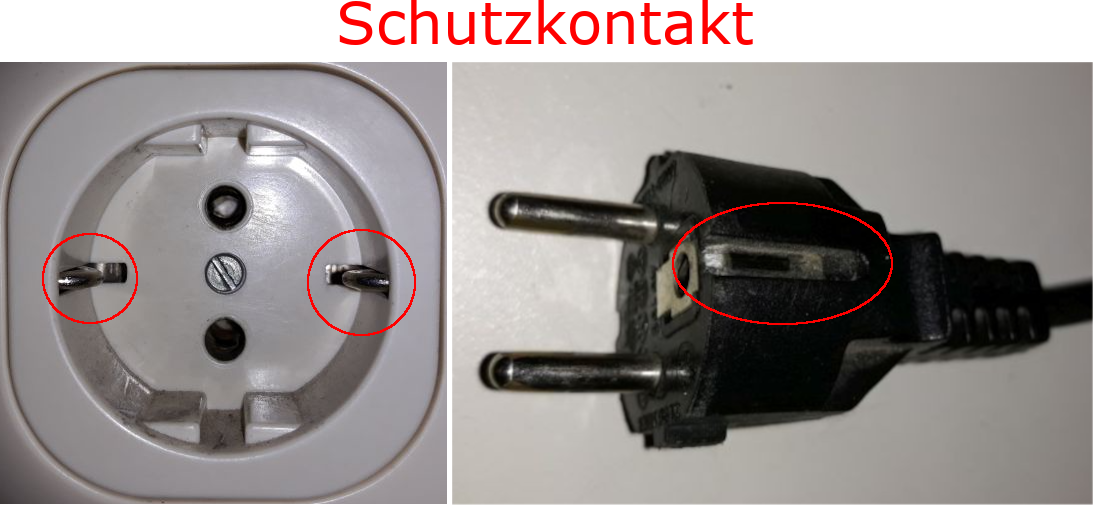
\includegraphics[width=0.85\textwidth]{foto/86}
    \caption{\scriptsize Schutzkontakt an einer Steckdose und Schukostecker}
    \label{n_schutzkontakt}
\end{figure}

   \end{column}
\end{columns}

\end{frame}

\begin{frame}
\only<1>{
\begin{QQuestion}{ND109}{Welche Verbindung stellt der Schutzkontakt in einem Schutzkontakt-Stecker (Schuko-Stecker) her?}{Verbindung zum L-Leiter der Steckdose}
{Verbindung zwischen PE- und N-Leiter in der Steckdose}
{Verbindung zum N-Leiter der Steckdose}
{Verbindung zum PE-Leiter der Steckdose}
\end{QQuestion}

}
\only<2>{
\begin{QQuestion}{ND109}{Welche Verbindung stellt der Schutzkontakt in einem Schutzkontakt-Stecker (Schuko-Stecker) her?}{Verbindung zum L-Leiter der Steckdose}
{Verbindung zwischen PE- und N-Leiter in der Steckdose}
{Verbindung zum N-Leiter der Steckdose}
{\textbf{\textcolor{DARCgreen}{Verbindung zum PE-Leiter der Steckdose}}}
\end{QQuestion}

}
\end{frame}

\begin{frame}
\frametitle{Gleichspannungsausgang}

\begin{figure}
    \DARCimage{0.85\linewidth}{680include}
    \caption{\scriptsize Anschluss von Netzgerät und TRX}
    \label{n_Netzgeraet_TRX}
\end{figure}
\begin{columns}
    \begin{column}{0.48\textwidth}
    \begin{itemize}
  \item Ist zweipolig zum Transceiver
  \item Klemmen sind in der Regel farbig
  \end{itemize}

    \end{column}
   \begin{column}{0.48\textwidth}
       
    \pause
    \begin{itemize}
  \item Rot für Plus
  \item Schwarz für Minus
  \item Polung beachten!
  \end{itemize}



   \end{column}
\end{columns}

\end{frame}

\begin{frame}
\only<1>{
\begin{QQuestion}{ND104}{Warum ist die Spannungsversorgungsleitung vom externen Netzteil zum Transceiver zweipolig ausgeführt?}{Damit die Spannungsreduzierung nicht zu hoch wird.}
{Damit von beiden Polen des Netzteils der Strom zum Transceiver fließen kann.}
{Der Transceiver nutzt eine Leitung, die andere Leitung dient zur Erdung.
}
{Damit der Stromkreis über den Transceiver geschlossen werden kann.}
\end{QQuestion}

}
\only<2>{
\begin{QQuestion}{ND104}{Warum ist die Spannungsversorgungsleitung vom externen Netzteil zum Transceiver zweipolig ausgeführt?}{Damit die Spannungsreduzierung nicht zu hoch wird.}
{Damit von beiden Polen des Netzteils der Strom zum Transceiver fließen kann.}
{Der Transceiver nutzt eine Leitung, die andere Leitung dient zur Erdung.
}
{\textbf{\textcolor{DARCgreen}{Damit der Stromkreis über den Transceiver geschlossen werden kann.}}}
\end{QQuestion}

}
\end{frame}

\begin{frame}
\only<1>{
\begin{QQuestion}{ND103}{Warum ist die Spannungsversorgungsleitung vom Gleichspannungsnetzteil zum Transceiver zweipolig ausgeführt?}{Der Strom fließt in beide Leiter hinein und über die Erde zum Netzteil zurück.}
{Der Strom fließt in einem Leiter hin und im anderen Leiter wieder zurück.}
{Damit insgesamt mehr Strom fließen kann.}
{Der Strom fließt aus beiden Leitern heraus und über die Erde zum Netzteil zurück.}
\end{QQuestion}

}
\only<2>{
\begin{QQuestion}{ND103}{Warum ist die Spannungsversorgungsleitung vom Gleichspannungsnetzteil zum Transceiver zweipolig ausgeführt?}{Der Strom fließt in beide Leiter hinein und über die Erde zum Netzteil zurück.}
{\textbf{\textcolor{DARCgreen}{Der Strom fließt in einem Leiter hin und im anderen Leiter wieder zurück.}}}
{Damit insgesamt mehr Strom fließen kann.}
{Der Strom fließt aus beiden Leitern heraus und über die Erde zum Netzteil zurück.}
\end{QQuestion}

}
\end{frame}

\begin{frame}
\only<1>{
\begin{QQuestion}{ND105}{Wie sind die Klemmen einer \qty{13,8}{\V} Gleichspannungsversorgung gekennzeichnet?}{Pluspol schwarz, Minuspol grüngelb}
{Pluspol blau, Minuspol rot}
{Pluspol rot, Minuspol schwarz}
{Pluspol braun, Minuspol grüngelb}
\end{QQuestion}

}
\only<2>{
\begin{QQuestion}{ND105}{Wie sind die Klemmen einer \qty{13,8}{\V} Gleichspannungsversorgung gekennzeichnet?}{Pluspol schwarz, Minuspol grüngelb}
{Pluspol blau, Minuspol rot}
{\textbf{\textcolor{DARCgreen}{Pluspol rot, Minuspol schwarz}}}
{Pluspol braun, Minuspol grüngelb}
\end{QQuestion}

}
\end{frame}

\begin{frame}
\only<1>{
\begin{QQuestion}{ND106}{Worauf ist beim Anschluss eines Gleichspannungsnetzteils an einen Transceiver  besonders zu achten?}{Korrekte Verbindung zur Antenne}
{Richtige Polung des Schutzkontaktsteckers}
{Polungsrichtiger Anschluss der Stromversorgungsleitung zum Transceiver}
{Polungsrichtiger Anschluss des SWR-Meters}
\end{QQuestion}

}
\only<2>{
\begin{QQuestion}{ND106}{Worauf ist beim Anschluss eines Gleichspannungsnetzteils an einen Transceiver  besonders zu achten?}{Korrekte Verbindung zur Antenne}
{Richtige Polung des Schutzkontaktsteckers}
{\textbf{\textcolor{DARCgreen}{Polungsrichtiger Anschluss der Stromversorgungsleitung zum Transceiver}}}
{Polungsrichtiger Anschluss des SWR-Meters}
\end{QQuestion}

}
\end{frame}

\begin{frame}
\only<1>{
\begin{QQuestion}{ND107}{Welche Folge kann eine Verpolung der Leitung vom Netzteil zum Transceiver nach sich ziehen?}{Ausfall der Backup-Batterie im Transceiver}
{Verzerrung des Sendesignals}
{Beschädigung des Funkgeräts}
{Verzerrung des Empfangssignals}
\end{QQuestion}

}
\only<2>{
\begin{QQuestion}{ND107}{Welche Folge kann eine Verpolung der Leitung vom Netzteil zum Transceiver nach sich ziehen?}{Ausfall der Backup-Batterie im Transceiver}
{Verzerrung des Sendesignals}
{\textbf{\textcolor{DARCgreen}{Beschädigung des Funkgeräts}}}
{Verzerrung des Empfangssignals}
\end{QQuestion}

}
\end{frame}

\begin{frame}
\frametitle{Feinsicherungen}
\begin{columns}
    \begin{column}{0.48\textwidth}
    
\begin{figure}
    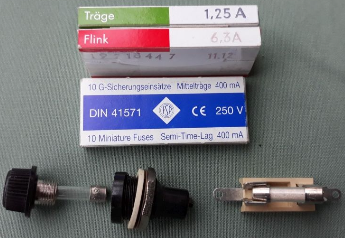
\includegraphics[width=0.85\textwidth]{foto/88}
    \caption{\scriptsize Feinsicherungen}
    \label{n_feinsicherungen}
\end{figure}

    \end{column}
   \begin{column}{0.48\textwidth}
       \begin{itemize}
  \item Unterbrechen Stromfluss im Fehlerfall (Kurzschluss oder Überlastung)
  \item Schmelzsicherungen in denen ein dünner Draht schmilzt
  \item \emph{Durchgebrannte Sicherung} bzw. \emph{thermische Abschaltung}
  \end{itemize}

   \end{column}
\end{columns}

\end{frame}

\begin{frame}
\frametitle{Feinsicherungen austauschen}
\begin{itemize}
  \item Erst die Ursache beheben
  \item Durch gleichartige ersetzen
  \item Stromstärke und Auslösecharakteristik
  \end{itemize}
\end{frame}

\begin{frame}
\frametitle{Kenngrößen von Feinsicherungen}
\begin{table}
\begin{DARCtabular}{ccc}
     Auslösecharakteristik  & Kennzeichen  & Abschaltzeit bei zehnfachem Nennstrom   \\
     flink  & F  & max. 30 ms  \\
     mittelträge  & MT  & max. 90 ms   \\
     träge  & T  & max. 300 ms   \\
\end{DARCtabular}
\caption{Kenngrößen von Feinsicherungen}
\label{n_feinsicherung}
\end{table}
\end{frame}

\begin{frame}
\frametitle{Elektronische Begrenzung}
\begin{itemize}
  \item In hochwertigen Netzgeräten
  \item Im Kurzschlussfall wird die Stromstärke begrenzt
  \item \emph{Kurzschlussstrombegrenzung}
  \item Kein Austausch von Sicherungen notwendig
  \end{itemize}
\end{frame}%ENDCONTENT


\section{Batterien und Akkus}
\label{section:batterien_und_akkus}
\begin{frame}%STARTCONTENT

\begin{columns}
    \begin{column}{0.48\textwidth}
    \begin{itemize}
  \item Spannung durch Ladungstrennung in elektrochemischen Vorgängen
  \item Beim Akku ist der Vorgang umkehrbar
  \item Plus- oder Minuspol gekennzeichnet
  \end{itemize}

    \end{column}
   \begin{column}{0.48\textwidth}
       
\begin{figure}
    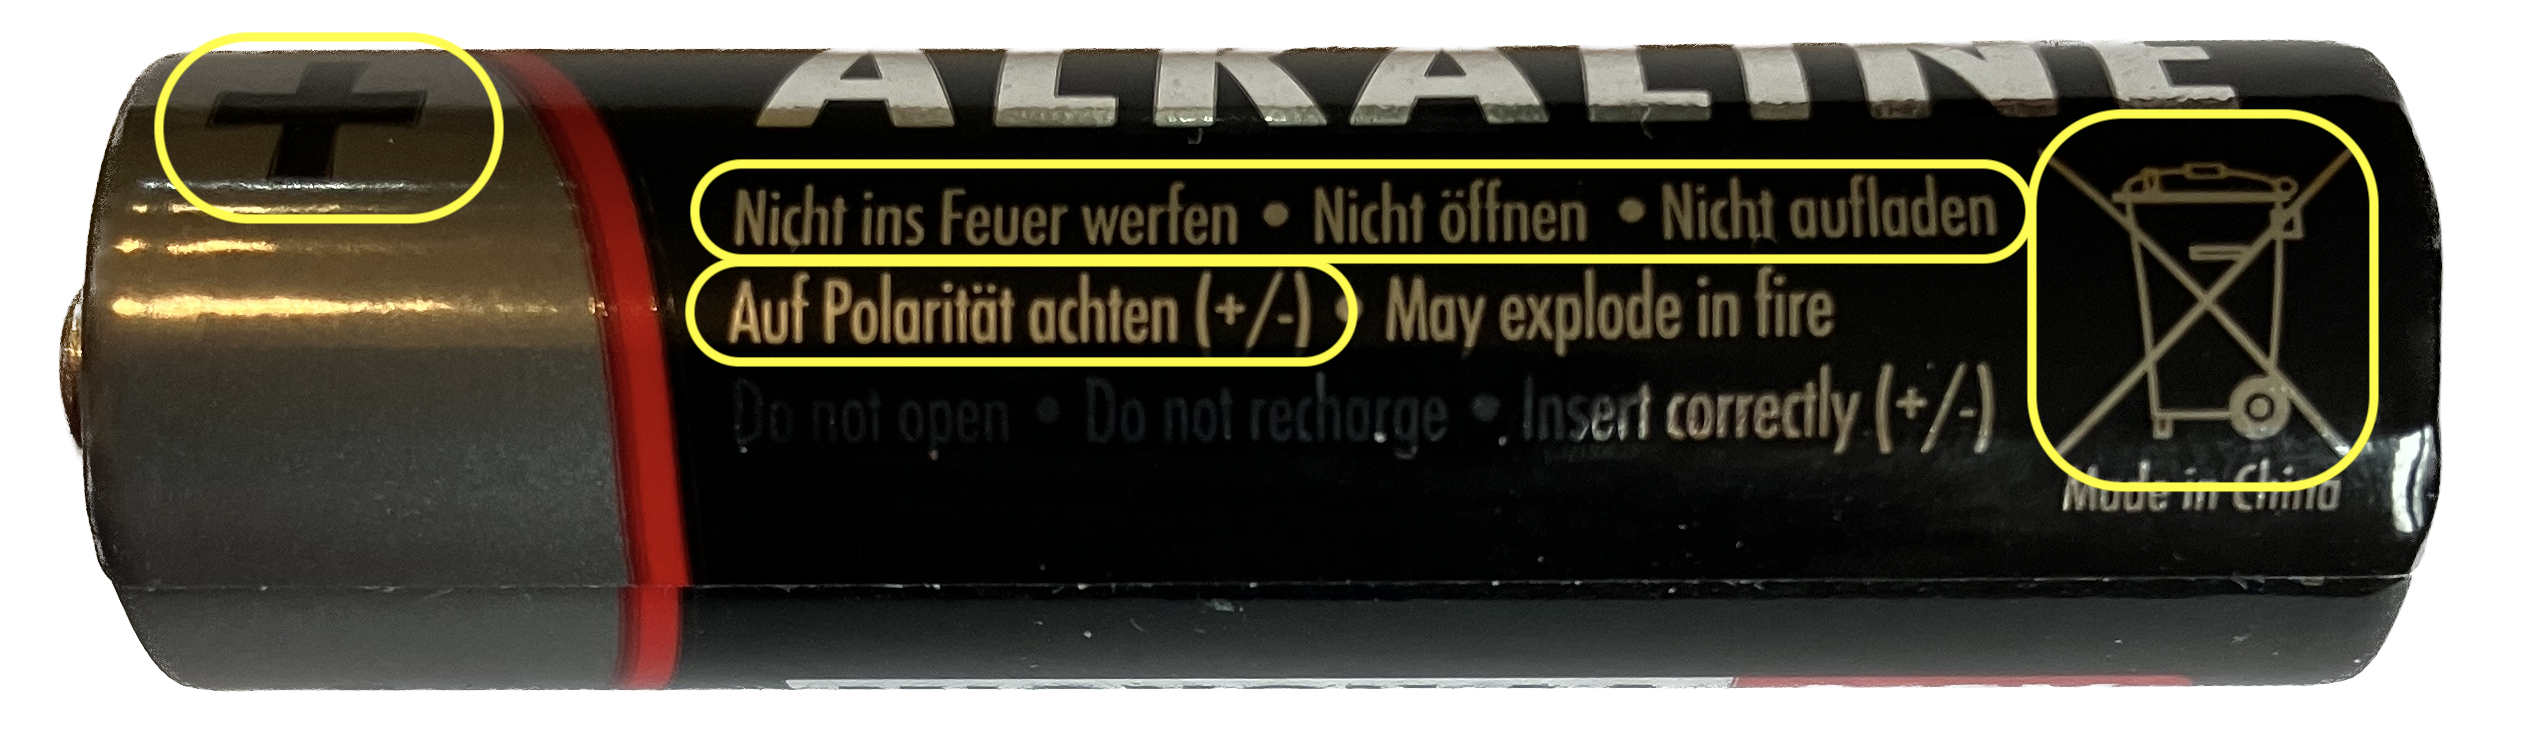
\includegraphics[width=0.85\textwidth]{foto/89}
    \caption{\scriptsize Eine Batterie mit Kennzeichnung der Pole und Warnhinweisen}
    \label{n_Bat_AA}
\end{figure}

\begin{figure}
    \DARCimage{0.85\linewidth}{517include}
    \caption{\scriptsize Schaltzeichen einer Batterie}
    \label{n_schaltzeichen_batt}
\end{figure}


   \end{column}
\end{columns}

\end{frame}

\begin{frame}
\only<1>{
\begin{PQuestion}{NB201}{Welches Bauteil wird durch das Schaltzeichen symbolisiert?}{Batterie}
{Diode}
{Widerstand}
{Kondensator}
{\DARCimage{0.5\linewidth}{510include}}\end{PQuestion}

}
\only<2>{
\begin{PQuestion}{NB201}{Welches Bauteil wird durch das Schaltzeichen symbolisiert?}{\textbf{\textcolor{DARCgreen}{Batterie}}}
{Diode}
{Widerstand}
{Kondensator}
{\DARCimage{0.5\linewidth}{510include}}\end{PQuestion}

}
\end{frame}

\begin{frame}
\only<1>{
\begin{PQuestion}{NB203}{Wie lauten die Bezeichnungen für die Anschlüsse 1 und 2 im Schaltsymbol?}{1 = Nord-Pol; 2 = Süd-Pol}
{1 = Minus-Pol; 2 = Plus-Pol}
{1 = Plus-Pol; 2 = Minus-Pol}
{1 = Süd-Pol; 2 = Nord-Pol}
{\DARCimage{0.5\linewidth}{517include}}\end{PQuestion}

}
\only<2>{
\begin{PQuestion}{NB203}{Wie lauten die Bezeichnungen für die Anschlüsse 1 und 2 im Schaltsymbol?}{1 = Nord-Pol; 2 = Süd-Pol}
{1 = Minus-Pol; 2 = Plus-Pol}
{\textbf{\textcolor{DARCgreen}{1 = Plus-Pol; 2 = Minus-Pol}}}
{1 = Süd-Pol; 2 = Nord-Pol}
{\DARCimage{0.5\linewidth}{517include}}\end{PQuestion}

}
\end{frame}

\begin{frame}
\frametitle{Serienschaltung}
\begin{columns}
    \begin{column}{0.48\textwidth}
    \begin{itemize}
  \item Batterien lassen sich hintereinander schalten
  \item Pluspol auf Minuspol der vorhergehenden Batterie
  \item Die Gesamtspannung ist die Summe der Einzelspannungen
  \end{itemize}

    \end{column}
   \begin{column}{0.48\textwidth}
       
\begin{figure}
    \DARCimage{0.85\linewidth}{748include}
    \caption{\scriptsize Verschiedene Batterien und Akkus}
    \label{batterien_und_akkus_sammlung}
\end{figure}


   \end{column}
\end{columns}

\end{frame}

\begin{frame}
\only<1>{
\begin{PQuestion}{NB204}{Folgende Schaltung besteht aus Spannungsquellen von je \qty{1,5}{\V}. Welche Spannung misst man zwischen den Kontakten, die mit \glqq +\grqq{} und \glqq -\grqq{} gekennzeichnet sind?}{\qty{0,25}{\V}}
{\qty{1,5}{\V}}
{\qty{9}{\V}}
{\qty{6}{\V}}
{\DARCimage{1.0\linewidth}{431include}}\end{PQuestion}

}
\only<2>{
\begin{PQuestion}{NB204}{Folgende Schaltung besteht aus Spannungsquellen von je \qty{1,5}{\V}. Welche Spannung misst man zwischen den Kontakten, die mit \glqq +\grqq{} und \glqq -\grqq{} gekennzeichnet sind?}{\qty{0,25}{\V}}
{\qty{1,5}{\V}}
{\textbf{\textcolor{DARCgreen}{\qty{9}{\V}}}}
{\qty{6}{\V}}
{\DARCimage{1.0\linewidth}{431include}}\end{PQuestion}

}
\end{frame}

\begin{frame}
\frametitle{Kurzschluss}
\begin{itemize}
  \item Vermeiden!
  \item Bei Akkus Gefahr der Überhitzung
  \item Brandgefahr
  \end{itemize}
\end{frame}

\begin{frame}
\only<1>{
\begin{QQuestion}{ND110}{Was ist bei der Verwendung von Akkus und Batterien zu beachten?}{Sie müssen paarweise verwendet werden.}
{Ein Kurzschluss ist zu vermeiden.}
{Sie müssen mit einem Mindestentladestrom betrieben werden.}
{Sie sollen stets vollkommen entladen werden.}
\end{QQuestion}

}
\only<2>{
\begin{QQuestion}{ND110}{Was ist bei der Verwendung von Akkus und Batterien zu beachten?}{Sie müssen paarweise verwendet werden.}
{\textbf{\textcolor{DARCgreen}{Ein Kurzschluss ist zu vermeiden.}}}
{Sie müssen mit einem Mindestentladestrom betrieben werden.}
{Sie sollen stets vollkommen entladen werden.}
\end{QQuestion}

}
 \end{frame}

\begin{frame}
\frametitle{Unsachgemäßer Umgang}
\begin{itemize}
  \item In Akkus sind verschiedene chemische Technologien im Einsatz
  \item Beim Aufladen angepasste Ladegeräte verwenden
  \item Gefahr von Überhitzung, Explosion oder Brand
  \item Dadurch kann es zu Verbrennungen, Verätzungen und Vergiftungen kommen
  \end{itemize}
\end{frame}

\begin{frame}
\only<1>{
\begin{QQuestion}{NK306}{Welche Gefahren drohen dem Anwender bei unsachgemäßem Umgang mit wiederaufladbaren Batterien?}{Verätzungen, Spannungsschwankungen, Ruhestromanstieg}
{Überstrom, Unterspannung, Leistungsreduzierung}
{Verbrennungen, Verätzungen, Vergiftungen}
{Anstieg des Innenwiderstands, Spannungsschwankungen, Leistungsreduzierung}
\end{QQuestion}

}
\only<2>{
\begin{QQuestion}{NK306}{Welche Gefahren drohen dem Anwender bei unsachgemäßem Umgang mit wiederaufladbaren Batterien?}{Verätzungen, Spannungsschwankungen, Ruhestromanstieg}
{Überstrom, Unterspannung, Leistungsreduzierung}
{\textbf{\textcolor{DARCgreen}{Verbrennungen, Verätzungen, Vergiftungen}}}
{Anstieg des Innenwiderstands, Spannungsschwankungen, Leistungsreduzierung}
\end{QQuestion}

}
 \end{frame}%ENDCONTENT


\section{Akkus}
\label{section:akku}
\begin{frame}%STARTCONTENT

\only<1>{
\begin{PQuestion}{AB209}{Folgende Schaltung eines Akkus besteht aus Zellen von je \qty{2}{\V}. Jede Zelle kann \qty{10}{\A\hour} Ladung liefern. Welche Daten hat der Akku?}{\qty{2}{\V}/\qty{10}{\A\hour}}
{\qty{12}{\V}/\qty{60}{\A\hour}}
{\qty{12}{\V}/\qty{10}{\A\hour}}
{\qty{2}{\V}/\qty{60}{\A\hour}}
{\DARCimage{1.0\linewidth}{431include}}\end{PQuestion}

}
\only<2>{
\begin{PQuestion}{AB209}{Folgende Schaltung eines Akkus besteht aus Zellen von je \qty{2}{\V}. Jede Zelle kann \qty{10}{\A\hour} Ladung liefern. Welche Daten hat der Akku?}{\qty{2}{\V}/\qty{10}{\A\hour}}
{\qty{12}{\V}/\qty{60}{\A\hour}}
{\textbf{\textcolor{DARCgreen}{\qty{12}{\V}/\qty{10}{\A\hour}}}}
{\qty{2}{\V}/\qty{60}{\A\hour}}
{\DARCimage{1.0\linewidth}{431include}}\end{PQuestion}

}
\end{frame}

\begin{frame}
\frametitle{Lösungsweg}
\begin{itemize}
  \item gegeben: $U = 2V$
  \item gegeben: $Q = 10Ah$
  \item gegeben: $N = 6$
  \item gesucht: $U_{ges}, Q_{ges}$
  \end{itemize}
    \pause
    $U_{ges} = N \cdot U = 6 \cdot 2V = 12V$
    \pause
    $Q_{ges} = Q =10Ah$



\end{frame}

\begin{frame}
\only<1>{
\begin{QQuestion}{AB210}{Auf dem Akku-Pack eines Handfunksprechgerätes stehen folgende Angaben: \qty{7,4}{\V} - \qty{2200}{\milli\A\hour} - \qty{16,28}{\W\hour}. Welcher Begriff ist für die Angabe \qty{2200}{\milli\A\hour} zutreffend.}{Nennkapazität}
{Nennleistung}
{maximaler Ladestrom pro Stunde}
{maximaler Entladestrom pro Stunde}
\end{QQuestion}

}
\only<2>{
\begin{QQuestion}{AB210}{Auf dem Akku-Pack eines Handfunksprechgerätes stehen folgende Angaben: \qty{7,4}{\V} - \qty{2200}{\milli\A\hour} - \qty{16,28}{\W\hour}. Welcher Begriff ist für die Angabe \qty{2200}{\milli\A\hour} zutreffend.}{\textbf{\textcolor{DARCgreen}{Nennkapazität}}}
{Nennleistung}
{maximaler Ladestrom pro Stunde}
{maximaler Entladestrom pro Stunde}
\end{QQuestion}

}
\end{frame}

\begin{frame}
\only<1>{
\begin{QQuestion}{AB211}{Wie lange könnte man idealerweise mit einem voll geladenen Akku mit \qty{60}{\A\hour} einen Amateurfunkempfänger betreiben, bis dieser auf \qty{10}{\percent} seiner Kapazität entladen ist und einen Strom von \qty{0,8}{\A} aufnimmt?}{74~Stunden und 60~Minuten}
{43~Stunden und 12~Minuten}
{67~Stunden und 30~Minuten}
{48~Stunden und 0~Minuten}
\end{QQuestion}

}
\only<2>{
\begin{QQuestion}{AB211}{Wie lange könnte man idealerweise mit einem voll geladenen Akku mit \qty{60}{\A\hour} einen Amateurfunkempfänger betreiben, bis dieser auf \qty{10}{\percent} seiner Kapazität entladen ist und einen Strom von \qty{0,8}{\A} aufnimmt?}{74~Stunden und 60~Minuten}
{43~Stunden und 12~Minuten}
{\textbf{\textcolor{DARCgreen}{67~Stunden und 30~Minuten}}}
{48~Stunden und 0~Minuten}
\end{QQuestion}

}
\end{frame}

\begin{frame}
\frametitle{Lösungsweg}
\begin{itemize}
  \item gegeben: $Q_{max} = 60Ah$
  \item gegeben: $Q_{10\%} = 0,1 \cdot Q_{max} = 6Ah$
  \item gegeben: $I = 0,8A$
  \item gesucht: $t$
  \end{itemize}
    \pause
    $Q = I \cdot t \Rightarrow t = \frac{Q}{I} = \frac{Q_{max} -- Q_{10\%}}{I} = \frac{54Ah}{0,8A} = 67,5h$



\end{frame}

\begin{frame}
\only<1>{
\begin{QQuestion}{AB501}{Ein \qty{12}{\V} Akku hat eine Kapazität von \qty{5}{\A\hour}. Welcher speicherbaren Energie entspricht das?}{\qty{5,0}{\W\hour}}
{\qty{12,0}{\W\hour}}
{\qty{2,4}{\W\hour}}
{\qty{60,0}{\W\hour}}
\end{QQuestion}

}
\only<2>{
\begin{QQuestion}{AB501}{Ein \qty{12}{\V} Akku hat eine Kapazität von \qty{5}{\A\hour}. Welcher speicherbaren Energie entspricht das?}{\qty{5,0}{\W\hour}}
{\qty{12,0}{\W\hour}}
{\qty{2,4}{\W\hour}}
{\textbf{\textcolor{DARCgreen}{\qty{60,0}{\W\hour}}}}
\end{QQuestion}

}
\end{frame}

\begin{frame}
\frametitle{Lösungsweg}
\begin{itemize}
  \item gegeben: $U = 12V$
  \item gegeben: $Q = 5Ah$
  \item gesucht: $W$
  \end{itemize}
    \pause
    $W = P \cdot t = U \cdot I \cdot t = U \cdot Q = 12V \cdot 5Ah = 60,0Wh$



\end{frame}%ENDCONTENT


\section{Photovoltaik}
\label{section:photovoltaik}
\begin{frame}%STARTCONTENT

\only<1>{
\begin{QQuestion}{AB212}{Was ist die primäre Aufgabe einer Solarzelle?}{Die Umwandlung von elektrischer Energie in Strahlungsenergie.}
{Die Umwandlung von Strahlungsenergie in elektrische Energie.}
{Die Umwandlung von Strahlungsenergie in thermische Energie.}
{Die Umwandlung von thermischer Energie in Strahlungsenergie.}
\end{QQuestion}

}
\only<2>{
\begin{QQuestion}{AB212}{Was ist die primäre Aufgabe einer Solarzelle?}{Die Umwandlung von elektrischer Energie in Strahlungsenergie.}
{\textbf{\textcolor{DARCgreen}{Die Umwandlung von Strahlungsenergie in elektrische Energie.}}}
{Die Umwandlung von Strahlungsenergie in thermische Energie.}
{Die Umwandlung von thermischer Energie in Strahlungsenergie.}
\end{QQuestion}

}
\end{frame}

\begin{frame}
\only<1>{
\begin{PQuestion}{AD301}{Ein Photovoltaikmodul besteht aus vier parallel geschalteten Reihen von je 30 Solarzellen mit je Zelle \qty{0,6}{\V} Leerlaufspannung und \qty{1}{\A} Kurzschlussstrom. Welche Leerlaufspannung und welchen Kurzschlussstrom liefert das Modul?}{Leerlaufspannung: \qty{18}{\V}, Kurzschlussstrom: \qty{4}{\A}}
{Leerlaufspannung: \qty{18}{\V}, Kurzschlussstrom: \qty{30}{\A}}
{Leerlaufspannung: \qty{2,4}{\V}, Kurzschlussstrom: \qty{4}{\A}}
{Leerlaufspannung: \qty{2,4}{\V}, Kurzschlussstrom: \qty{30}{\A}}
{\DARCimage{1.0\linewidth}{46include}}\end{PQuestion}

}
\only<2>{
\begin{PQuestion}{AD301}{Ein Photovoltaikmodul besteht aus vier parallel geschalteten Reihen von je 30 Solarzellen mit je Zelle \qty{0,6}{\V} Leerlaufspannung und \qty{1}{\A} Kurzschlussstrom. Welche Leerlaufspannung und welchen Kurzschlussstrom liefert das Modul?}{\textbf{\textcolor{DARCgreen}{Leerlaufspannung: \qty{18}{\V}, Kurzschlussstrom: \qty{4}{\A}}}}
{Leerlaufspannung: \qty{18}{\V}, Kurzschlussstrom: \qty{30}{\A}}
{Leerlaufspannung: \qty{2,4}{\V}, Kurzschlussstrom: \qty{4}{\A}}
{Leerlaufspannung: \qty{2,4}{\V}, Kurzschlussstrom: \qty{30}{\A}}
{\DARCimage{1.0\linewidth}{46include}}\end{PQuestion}

}
\end{frame}

\begin{frame}
\frametitle{Lösungweg}
\begin{itemize}
  \item gegeben: $U_0 = 0,6V$
  \item gegeben: $I_k = 1A$
  \item gegeben: $N_R = 30, N_P = 4$
  \item gesucht: $U_{0,ges}, I_{k,ges}$
  \end{itemize}
    \pause
    $U_{0,ges} = N_R \cdot U_0 = 30 \cdot 0,6V = 18V$
    \pause
    $I_{0,ges} = N_P \cdot I_k = 4 \cdot 1A = 4A$



\end{frame}%ENDCONTENT


\section{Spannungswandler}
\label{section:spannungswandler}
\begin{frame}%STARTCONTENT
\end{frame}%ENDCONTENT


\section{Gleichrichter I}
\label{section:gleichrichter_1}
\begin{frame}%STARTCONTENT

\frametitle{Gleichrichter}
\begin{columns}
    \begin{column}{0.48\textwidth}
    \begin{itemize}
  \item Um die Wechselspannung zu einer Gleichspannung zu wandeln, benötigen wir einen Gleichrichter.
  \item Die einfachste Möglichkeit ist die Gleichrichtung mit einer Diode, denn eine Diode leitet den Strom nur in eine Richtung.
  \end{itemize}

    \end{column}
   \begin{column}{0.48\textwidth}
       
\begin{figure}
    \DARCimage{0.85\linewidth}{797include}
    \caption{\scriptsize Einweggleichrichter}
    \label{e_einweggleichrichter}
\end{figure}


   \end{column}
\end{columns}

\end{frame}

\begin{frame}
\begin{columns}
    \begin{column}{0.48\textwidth}
    \begin{itemize}
  \item Damit \enquote{schneiden} wir von der Wechselspannung die negative Halbwelle ab.
  \item Weitere Bauelemente sind notwendig um aus den positiven Halbwellen eine stabile Gleichspannung zu machen, diese lernen wir im Klasse~A Kurs kennen.
  \end{itemize}

    \end{column}
   \begin{column}{0.48\textwidth}
       
\begin{figure}
    \DARCimage{0.85\linewidth}{798include}
    \caption{\scriptsize Eingangsspannung Einweggleichrichter}
    \label{e_einweggleichrichter_ue}
\end{figure}


\begin{figure}
    \DARCimage{0.85\linewidth}{796include}
    \caption{\scriptsize Lastspannung Einweggleichrichter}
    \label{e_einweggleichrichter_ul}
\end{figure}


   \end{column}
\end{columns}

\end{frame}

\begin{frame}
\only<1>{
\begin{PQuestion}{ED304}{Welchen Verlauf hat die Spannung $U$?}{\DARCimage{1.0\linewidth}{215include}}
{\DARCimage{1.0\linewidth}{214include}}
{\DARCimage{1.0\linewidth}{216include}}
{\DARCimage{1.0\linewidth}{217include}}
{\DARCimage{1.0\linewidth}{304include}}\end{PQuestion}

}
\only<2>{
\begin{PQuestion}{ED304}{Welchen Verlauf hat die Spannung $U$?}{\DARCimage{1.0\linewidth}{215include}}
{\textbf{\textcolor{DARCgreen}{\DARCimage{1.0\linewidth}{214include}}}}
{\DARCimage{1.0\linewidth}{216include}}
{\DARCimage{1.0\linewidth}{217include}}
{\DARCimage{1.0\linewidth}{304include}}\end{PQuestion}

}
\end{frame}%ENDCONTENT


\section{Gleichrichter II}
\label{section:gleichrichter_2}
\begin{frame}%STARTCONTENT

\only<1>{
\begin{PQuestion}{AD302}{Berechnen Sie für diese Schaltung die Leerlaufspannung an den Klemmen A - B.}{Zirka \qty{42}{\V}}
{Zirka \qty{15}{\V}}
{Zirka \qty{30}{\V}}
{Zirka \qty{21}{\V}}
{\DARCimage{1.0\linewidth}{198include}}\end{PQuestion}

}
\only<2>{
\begin{PQuestion}{AD302}{Berechnen Sie für diese Schaltung die Leerlaufspannung an den Klemmen A - B.}{Zirka \qty{42}{\V}}
{Zirka \qty{15}{\V}}
{Zirka \qty{30}{\V}}
{\textbf{\textcolor{DARCgreen}{Zirka \qty{21}{\V}}}}
{\DARCimage{1.0\linewidth}{198include}}\end{PQuestion}

}
\end{frame}

\begin{frame}
\frametitle{Lösungsweg}
\begin{itemize}
  \item gegeben: $U_{eff} = 15V$
  \item gesucht: $\hat{U}$
  \end{itemize}
    \pause
    $\hat{U} = U_{eff} \cdot \sqrt{2} = 15V \cdot 1,41 = 21,21V$



\end{frame}

\begin{frame}
\only<1>{
\begin{PQuestion}{AD303}{Welche Spannungsfestigkeit des Kondensators sollte mindestens gewählt werden, wenn das Transformationsverhältnis 20:1 beträgt und ein Sicherheitsaufschlag auf die Spannungsfestigkeit von \qty{50}{\percent} berücksichtigt werden soll?}{\qty{35}{\V}}
{\qty{16}{\V} }
{\qty{25}{\V} }
{\qty{10}{\V}}
{\DARCimage{1.0\linewidth}{29include}}\end{PQuestion}

}
\only<2>{
\begin{PQuestion}{AD303}{Welche Spannungsfestigkeit des Kondensators sollte mindestens gewählt werden, wenn das Transformationsverhältnis 20:1 beträgt und ein Sicherheitsaufschlag auf die Spannungsfestigkeit von \qty{50}{\percent} berücksichtigt werden soll?}{\qty{35}{\V}}
{\qty{16}{\V} }
{\textbf{\textcolor{DARCgreen}{\qty{25}{\V} }}}
{\qty{10}{\V}}
{\DARCimage{1.0\linewidth}{29include}}\end{PQuestion}

}
\end{frame}

\begin{frame}
\frametitle{Lösungsweg}
\begin{itemize}
  \item gegeben: $U_P = 230V$
  \item gegeben: $\"{u} = 20:1$
  \item gesucht: $\hat{U} + 50\%$
  \end{itemize}
    \pause
    $ü = \frac{U_P}{U_S} \Rightarrow U_S = \frac{U_P}{ü} = \frac{230V}{20} = 11,5V$
    \pause
    $\hat{U} = U_S \cdot \sqrt{2} = 11,5V \cdot 1,41 \approx 16,26V$
    \pause
    $\hat{U} + 50\% \approx 25V$



\end{frame}

\begin{frame}
\only<1>{
\begin{PQuestion}{AD304}{Bei einem Transformationsverhältnis von 5:1 sollte die Spannungsfestigkeit der Diode (max. Spannung plus \qty{20}{\percent} Sicherheitsaufschlag) in dieser Schaltung nicht weniger als~...}{\qty{90}{\V} betragen.}
{\qty{78}{\V} betragen.}
{\qty{156}{\V} betragen.}
{\qty{130}{\V} betragen.}
{\DARCimage{1.0\linewidth}{29include}}\end{PQuestion}

}
\only<2>{
\begin{PQuestion}{AD304}{Bei einem Transformationsverhältnis von 5:1 sollte die Spannungsfestigkeit der Diode (max. Spannung plus \qty{20}{\percent} Sicherheitsaufschlag) in dieser Schaltung nicht weniger als~...}{\qty{90}{\V} betragen.}
{\qty{78}{\V} betragen.}
{\textbf{\textcolor{DARCgreen}{\qty{156}{\V} betragen.}}}
{\qty{130}{\V} betragen.}
{\DARCimage{1.0\linewidth}{29include}}\end{PQuestion}

}
\end{frame}

\begin{frame}
\frametitle{Lösungsweg}
\begin{itemize}
  \item gegeben: $U_P = 230V$
  \item gegeben: $\"{u} = 5:1$
  \item gesucht: $U_{SS} + 20\%$
  \end{itemize}
    \pause
    $ü = \frac{U_P}{U_S} \Rightarrow U_S = \frac{U_P}{ü} = \frac{230V}{5} = 46V$
    \pause
    $\hat{U} = U_S \cdot \sqrt{2} = 46V \cdot 1,41 \approx 65,05V$
    \pause
    $U_{SS} + 20\% = 2 \cdot \hat{U} + 20\% \approx 156V$



\end{frame}%ENDCONTENT


\section{Brückengleichrichter}
\label{section:brueckengleichrichter}
\begin{frame}%STARTCONTENT

\only<1>{
\begin{question2x2}{AD305}{Welche der folgenden Auswahlantworten enthält die richtige Diodenanordnung und Polarität eines Brückengleichrichters?}{\DARCimage{1.0\linewidth}{69include}}
{\DARCimage{1.0\linewidth}{68include}}
{\DARCimage{1.0\linewidth}{67include}}
{\DARCimage{1.0\linewidth}{70include}}
\end{question2x2}

}
\only<2>{
\begin{question2x2}{AD305}{Welche der folgenden Auswahlantworten enthält die richtige Diodenanordnung und Polarität eines Brückengleichrichters?}{\DARCimage{1.0\linewidth}{69include}}
{\DARCimage{1.0\linewidth}{68include}}
{\textbf{\textcolor{DARCgreen}{\DARCimage{1.0\linewidth}{67include}}}}
{\DARCimage{1.0\linewidth}{70include}}
\end{question2x2}

}
\end{frame}

\begin{frame}
\only<1>{
\begin{PQuestion}{AD306}{Wie groß ist die Spannung am Siebkondensator $C_{\symup{S}}$ im Leerlauf, wenn die Netzwechselspannung von \qty{230}{\V} anliegt und das Windungsverhältnis 8:1 beträgt?}{etwa \qty{20}{\V}}
{etwa \qty{40}{\V}}
{etwa \qty{29}{\V}}
{etwa \qty{58}{\V}}
{\DARCimage{1.0\linewidth}{66include}}\end{PQuestion}

}
\only<2>{
\begin{PQuestion}{AD306}{Wie groß ist die Spannung am Siebkondensator $C_{\symup{S}}$ im Leerlauf, wenn die Netzwechselspannung von \qty{230}{\V} anliegt und das Windungsverhältnis 8:1 beträgt?}{etwa \qty{20}{\V}}
{\textbf{\textcolor{DARCgreen}{etwa \qty{40}{\V}}}}
{etwa \qty{29}{\V}}
{etwa \qty{58}{\V}}
{\DARCimage{1.0\linewidth}{66include}}\end{PQuestion}

}
\end{frame}

\begin{frame}
\frametitle{Lösungsweg}
\begin{itemize}
  \item gegeben: $U_P = 230V$
  \item gegeben: $\"{u} = 8:1$
  \item gegeben: $U_D = 0,6V$
  \item gesucht: $\hat{U}$
  \end{itemize}
    \pause
    $ü = \frac{U_P}{U_S} \Rightarrow U_S = \frac{U_P}{ü} = \frac{230V}{8} = 28,75V$
    \pause
    Im Leerlauf kann die Diodenspannung vernachlässigt werden.

$\hat{U} = U_S \cdot \sqrt{2} = 28,75V \cdot 1,41 \approx 40V$



\end{frame}%ENDCONTENT


\section{Vollweggleichrichter}
\label{section:vollweggleichrichter}
\begin{frame}%STARTCONTENT

\only<1>{
\begin{question2x2}{AD307}{Welche Gleichrichterschaltung erzeugt eine Vollweg-Gleichrichtung mit der angezeigten Polarität?}{\DARCimage{1.0\linewidth}{72include}}
{\DARCimage{1.0\linewidth}{71include}}
{\DARCimage{1.0\linewidth}{73include}}
{\DARCimage{1.0\linewidth}{74include}}
\end{question2x2}

}
\only<2>{
\begin{question2x2}{AD307}{Welche Gleichrichterschaltung erzeugt eine Vollweg-Gleichrichtung mit der angezeigten Polarität?}{\DARCimage{1.0\linewidth}{72include}}
{\textbf{\textcolor{DARCgreen}{\DARCimage{1.0\linewidth}{71include}}}}
{\DARCimage{1.0\linewidth}{73include}}
{\DARCimage{1.0\linewidth}{74include}}
\end{question2x2}

}
\end{frame}

\begin{frame}
\only<1>{
\begin{PQuestion}{AD308}{Welche Form hat die Ausgangsspannung der dargestellten Schaltung?}{\DARCimage{1\linewidth}{64include}}
{\DARCimage{1\linewidth}{62include}}
{\DARCimage{1\linewidth}{63include}}
{\DARCimage{1\linewidth}{61include}}
{\DARCimage{1\linewidth}{65include}}\end{PQuestion}

}
\only<2>{
\begin{PQuestion}{AD308}{Welche Form hat die Ausgangsspannung der dargestellten Schaltung?}{\DARCimage{1\linewidth}{64include}}
{\DARCimage{1\linewidth}{62include}}
{\DARCimage{1\linewidth}{63include}}
{\textbf{\textcolor{DARCgreen}{\DARCimage{1\linewidth}{61include}}}}
{\DARCimage{1\linewidth}{65include}}\end{PQuestion}

}
\end{frame}

\begin{frame}
\only<1>{
\begin{QQuestion}{AD310}{Welche Grundfrequenz hat die Ausgangsspannung eines Vollweggleichrichters, der an eine \qty{50}{\Hz}-Versorgung angeschlossen ist?}{\qty{100}{\Hz}}
{\qty{50}{\Hz}}
{\qty{25}{\Hz}}
{\qty{200}{\Hz}}
\end{QQuestion}

}
\only<2>{
\begin{QQuestion}{AD310}{Welche Grundfrequenz hat die Ausgangsspannung eines Vollweggleichrichters, der an eine \qty{50}{\Hz}-Versorgung angeschlossen ist?}{\textbf{\textcolor{DARCgreen}{\qty{100}{\Hz}}}}
{\qty{50}{\Hz}}
{\qty{25}{\Hz}}
{\qty{200}{\Hz}}
\end{QQuestion}

}
\end{frame}%ENDCONTENT


\section{Restwelligkeit}
\label{section:restwelligkeit}
\begin{frame}%STARTCONTENT

\only<1>{
\begin{PQuestion}{AD309}{Im folgenden Bild ist die Spannung am Ausgang einer Stromversorgung dargestellt. Die Restwelligkeit und die Brummfrequenz betragen~...}{\qty{3}{\V}; \qty{50}{\Hz}}
{\qty{3}{\V}; \qty{100}{\Hz}}
{\qty{13,5}{\V}~\pm\qty{1,5}{\V}; \qty{50}{\Hz}}
{\qty{13,5}{\V}~\pm\qty{1,5}{\V}; \qty{100}{\Hz}}
{\DARCimage{1.0\linewidth}{75include}}\end{PQuestion}

}
\only<2>{
\begin{PQuestion}{AD309}{Im folgenden Bild ist die Spannung am Ausgang einer Stromversorgung dargestellt. Die Restwelligkeit und die Brummfrequenz betragen~...}{\qty{3}{\V}; \qty{50}{\Hz}}
{\textbf{\textcolor{DARCgreen}{\qty{3}{\V}; \qty{100}{\Hz}}}}
{\qty{13,5}{\V}~\pm\qty{1,5}{\V}; \qty{50}{\Hz}}
{\qty{13,5}{\V}~\pm\qty{1,5}{\V}; \qty{100}{\Hz}}
{\DARCimage{1.0\linewidth}{75include}}\end{PQuestion}

}
\end{frame}%ENDCONTENT


\section{Schaltnetzteil I}
\label{section:schaltnetzteil_1}
\begin{frame}%STARTCONTENT
\begin{itemize}
  \item Das im vorigen Kapitel vorgestellte Netzteil hat den Nachteil eines hohen Gewichts durch den Transformator und einen schlechten Wirkungsgrad aufgrund von Verlusten bei der Konstanthaltung der Ausgangsspannung.
  \item Schaltnetzteile bringen die Eingangsspannung auf eine höhere Frequenz, wodurch kleinere Transformatoren eingesetzt werden können und bieten effizientere Wege die Ausgangsspannung konstant zu halten.
  \end{itemize}
\end{frame}

\begin{frame}Details auch hier im Klasse~A Kurs, wir konzentrieren uns auf die positiven Eigenschaften:

\begin{itemize}
  \item \emph{Hoher Wirkungsgrad}
  \item \emph{Geringes Gewicht}
  \item \emph{Geringes Volumen}
  \end{itemize}
\end{frame}

\begin{frame}
\only<1>{
\begin{QQuestion}{ED302}{Welche Eigenschaften hat ein Schaltnetzteil?}{Hoher Wirkungsgrad, geringes Gewicht, geringes Volumen.}
{Niedriger Wirkungsgrad, geringes Gewicht, geringes Volumen.}
{Hoher Wirkungsgrad, hohes Gewicht, geringes Volumen.}
{Hoher Wirkungsgrad, geringes Gewicht, großes Volumen.}
\end{QQuestion}

}
\only<2>{
\begin{QQuestion}{ED302}{Welche Eigenschaften hat ein Schaltnetzteil?}{\textbf{\textcolor{DARCgreen}{Hoher Wirkungsgrad, geringes Gewicht, geringes Volumen.}}}
{Niedriger Wirkungsgrad, geringes Gewicht, geringes Volumen.}
{Hoher Wirkungsgrad, hohes Gewicht, geringes Volumen.}
{Hoher Wirkungsgrad, geringes Gewicht, großes Volumen.}
\end{QQuestion}

}
\end{frame}

\begin{frame}Aber: Wo Licht ist, ist auch Schatten.

\begin{itemize}
  \item Durch die hohen Frequenzen kann es zu \emph{hochfrequenten Störungen} kommen, die besonders im Kurzwellenbereich stören.
  \item Bei für den Amateurfunk konzipierten Netzgeräten ist das inzwischen kein Problem mehr, bei Netzgeräten in der Unterhaltungselektronik schon.
  \end{itemize}
\end{frame}

\begin{frame}
\only<1>{
\begin{QQuestion}{ED303}{Welches ist der Hauptnachteil eines Schaltnetzteils ?}{Ein Schaltnetzteil kann keine so hohen Ströme abgeben.}
{Ein Schaltnetzteil hat einen niedrigen Wirkungsgrad.}
{Ein Schaltnetzteil kann hochfrequente Störungen erzeugen.}
{Ein Schaltnetzteil hat hohe Verluste.}
\end{QQuestion}

}
\only<2>{
\begin{QQuestion}{ED303}{Welches ist der Hauptnachteil eines Schaltnetzteils ?}{Ein Schaltnetzteil kann keine so hohen Ströme abgeben.}
{Ein Schaltnetzteil hat einen niedrigen Wirkungsgrad.}
{\textbf{\textcolor{DARCgreen}{Ein Schaltnetzteil kann hochfrequente Störungen erzeugen.}}}
{Ein Schaltnetzteil hat hohe Verluste.}
\end{QQuestion}

}
\end{frame}%ENDCONTENT


\section{Schaltnetzteil II}
\label{section:schaltnetzteil_2}
\begin{frame}%STARTCONTENT

\only<1>{
\begin{PQuestion}{AD311}{Welche Funktion übernimmt der elektronische Schalter (Block E) des Schaltnetzteils?}{Gleichrichter}
{Überspannungsableiter}
{Impulsbreitenmodulator}
{Puls-Gleichrichter}
{\DARCimage{1.0\linewidth}{35include}}\end{PQuestion}

}
\only<2>{
\begin{PQuestion}{AD311}{Welche Funktion übernimmt der elektronische Schalter (Block E) des Schaltnetzteils?}{Gleichrichter}
{Überspannungsableiter}
{\textbf{\textcolor{DARCgreen}{Impulsbreitenmodulator}}}
{Puls-Gleichrichter}
{\DARCimage{1.0\linewidth}{35include}}\end{PQuestion}

}
\end{frame}

\begin{frame}
\only<1>{
\begin{PQuestion}{AD312}{Was ist der Hauptnachteil des dargestellten Schaltnetzteils?}{Der Transformator bewirkt hohe Verluste}
{Der elektronische Schalter in Block E erzeugt ein unerwünschtes Signalspektrum.}
{Der Brückengleichrichter erzeugt eine Spannung mit Restwelligkeit.}
{Die Diode am Ausgang muss hohe Frequenzen gleichrichten.}
{\DARCimage{1.0\linewidth}{35include}}\end{PQuestion}

}
\only<2>{
\begin{PQuestion}{AD312}{Was ist der Hauptnachteil des dargestellten Schaltnetzteils?}{Der Transformator bewirkt hohe Verluste}
{\textbf{\textcolor{DARCgreen}{Der elektronische Schalter in Block E erzeugt ein unerwünschtes Signalspektrum.}}}
{Der Brückengleichrichter erzeugt eine Spannung mit Restwelligkeit.}
{Die Diode am Ausgang muss hohe Frequenzen gleichrichten.}
{\DARCimage{1.0\linewidth}{35include}}\end{PQuestion}

}
\end{frame}

\begin{frame}
\only<1>{
\begin{QQuestion}{AD313}{In einem Amateurfunkempfänger werden etwa alle \qty{120}{\kHz} unerwünschte Signale festgestellt. Dies ist wahrscheinlich zurückzuführen auf~...}{einen schlecht entstörten Bürstenmotor.}
{unerwünschte Abstrahlungen eines Schaltnetzteils.}
{unerwünschte Abstrahlungen eines linearen Netzteils.}
{eine Amateurfunkstelle mit unzureichender Anpassung der Antenne.}
\end{QQuestion}

}
\only<2>{
\begin{QQuestion}{AD313}{In einem Amateurfunkempfänger werden etwa alle \qty{120}{\kHz} unerwünschte Signale festgestellt. Dies ist wahrscheinlich zurückzuführen auf~...}{einen schlecht entstörten Bürstenmotor.}
{\textbf{\textcolor{DARCgreen}{unerwünschte Abstrahlungen eines Schaltnetzteils.}}}
{unerwünschte Abstrahlungen eines linearen Netzteils.}
{eine Amateurfunkstelle mit unzureichender Anpassung der Antenne.}
\end{QQuestion}

}
\end{frame}

\begin{frame}
\only<1>{
\begin{question2x2}{AD314}{Welche der dargestellten Schaltungen könnte in den Netzeingang eines Schaltnetzteils eingebaut werden, um eine Verbreitung von Störungen in das Stromversorgungsnetz zu verringern?}{\DARCimage{1.0\linewidth}{370include}}
{\DARCimage{1.0\linewidth}{368include}}
{\DARCimage{1.0\linewidth}{369include}}
{\DARCimage{1.0\linewidth}{367include}}
\end{question2x2}

}
\only<2>{
\begin{question2x2}{AD314}{Welche der dargestellten Schaltungen könnte in den Netzeingang eines Schaltnetzteils eingebaut werden, um eine Verbreitung von Störungen in das Stromversorgungsnetz zu verringern?}{\DARCimage{1.0\linewidth}{370include}}
{\DARCimage{1.0\linewidth}{368include}}
{\DARCimage{1.0\linewidth}{369include}}
{\textbf{\textcolor{DARCgreen}{\DARCimage{1.0\linewidth}{367include}}}}
\end{question2x2}

}
\end{frame}%ENDCONTENT


\section{Spannungsstabilisierung}
\label{section:spannungsstabilisierung}
\begin{frame}%STARTCONTENT

\only<1>{
\begin{PQuestion}{AD315}{Wenn man folgendes Signal an den Eingang der gezeigten Schaltung anlegt, beträgt die Ausgangsspannung zwischen A und B ungefähr~...}{\qty{6,2}{\V}.}
{\qty{11,2}{\V}.}
{\qty{5}{\V}.}
{\qty{5,6}{\V}.}
{\DARCimage{1.0\linewidth}{490include}}\end{PQuestion}

}
\only<2>{
\begin{PQuestion}{AD315}{Wenn man folgendes Signal an den Eingang der gezeigten Schaltung anlegt, beträgt die Ausgangsspannung zwischen A und B ungefähr~...}{\qty{6,2}{\V}.}
{\qty{11,2}{\V}.}
{\textbf{\textcolor{DARCgreen}{\qty{5}{\V}.}}}
{\qty{5,6}{\V}.}
{\DARCimage{1.0\linewidth}{490include}}\end{PQuestion}

}
\end{frame}

\begin{frame}
\only<1>{
\begin{PQuestion}{AD316}{Welche Beziehung muss zwischen der Eingangsspannung und der Ausgangsspannung der folgenden Schaltung bestehen, damit der Linearspannungsregler IC1 eine stabilisierte Ausgangsspannung erzeugt?}{Die Eingangsspannung muss gleich der gewünschten Ausgangsspannung sein}
{Die Eingangsspannung muss größer als die gewünschte Ausgangsspannung sein.}
{Die Eingangsspannung muss mindestens doppelt so groß wie die gewünschte Ausgangsspannung sein.}
{Die Eingangsspannung muss kleiner als die gewünschte Ausgangsspannung sein.}
{\DARCimage{1.0\linewidth}{200include}}\end{PQuestion}

}
\only<2>{
\begin{PQuestion}{AD316}{Welche Beziehung muss zwischen der Eingangsspannung und der Ausgangsspannung der folgenden Schaltung bestehen, damit der Linearspannungsregler IC1 eine stabilisierte Ausgangsspannung erzeugt?}{Die Eingangsspannung muss gleich der gewünschten Ausgangsspannung sein}
{\textbf{\textcolor{DARCgreen}{Die Eingangsspannung muss größer als die gewünschte Ausgangsspannung sein.}}}
{Die Eingangsspannung muss mindestens doppelt so groß wie die gewünschte Ausgangsspannung sein.}
{Die Eingangsspannung muss kleiner als die gewünschte Ausgangsspannung sein.}
{\DARCimage{1.0\linewidth}{200include}}\end{PQuestion}

}
\end{frame}

\begin{frame}
\only<1>{
\begin{PQuestion}{AD317}{Bei dieser Schaltung mit einem \qty{12}{\V}-Festspannungsregler schwankt die Eingangsspannung zwischen \qty{15}{\V} und \qty{18}{\V}. Wie groß ist die Spannungsschwankung am Ausgang?}{Die Spannungsschwankung beträgt ca.~\qty{3}{\V}.}
{Die Spannungsschwankung beträgt nahezu null Volt.}
{Die Spannungsschwankung beträgt ca.~\qty{0,7}{\V}.}
{Die Spannungsschwankung liegt zwischen \qty{0,7}{\V} und \qty{3}{\V}.}
{\DARCimage{1.0\linewidth}{200include}}\end{PQuestion}

}
\only<2>{
\begin{PQuestion}{AD317}{Bei dieser Schaltung mit einem \qty{12}{\V}-Festspannungsregler schwankt die Eingangsspannung zwischen \qty{15}{\V} und \qty{18}{\V}. Wie groß ist die Spannungsschwankung am Ausgang?}{Die Spannungsschwankung beträgt ca.~\qty{3}{\V}.}
{\textbf{\textcolor{DARCgreen}{Die Spannungsschwankung beträgt nahezu null Volt.}}}
{Die Spannungsschwankung beträgt ca.~\qty{0,7}{\V}.}
{Die Spannungsschwankung liegt zwischen \qty{0,7}{\V} und \qty{3}{\V}.}
{\DARCimage{1.0\linewidth}{200include}}\end{PQuestion}

}
\end{frame}

\begin{frame}
\only<1>{
\begin{QQuestion}{AD319}{Ein linearer Spannungsregler stabilisiert eine Eingangsspannung von \qty{13,8}{\V} auf eine Ausgangsspannung von \qty{9}{\V}. Es fließt ein Ausgangsstrom von \qty{900}{\mA}. Wie groß ist die Verlustleistung im Spannungsregler?}{\qty{12,42}{\W}}
{\qty{8,10}{\W}}
{\qty{4,32}{\W}}
{\qty{1,53}{\W}}
\end{QQuestion}

}
\only<2>{
\begin{QQuestion}{AD319}{Ein linearer Spannungsregler stabilisiert eine Eingangsspannung von \qty{13,8}{\V} auf eine Ausgangsspannung von \qty{9}{\V}. Es fließt ein Ausgangsstrom von \qty{900}{\mA}. Wie groß ist die Verlustleistung im Spannungsregler?}{\qty{12,42}{\W}}
{\qty{8,10}{\W}}
{\textbf{\textcolor{DARCgreen}{\qty{4,32}{\W}}}}
{\qty{1,53}{\W}}
\end{QQuestion}

}
\end{frame}

\begin{frame}
\frametitle{Lösungsweg}
\begin{itemize}
  \item gegeben: $U_{zu} = 13,8V$
  \item gegeben: $U_{ab} = 9V$
  \item gegeben: $I = 900mA$
  \item gesucht: $P_V$
  \end{itemize}
    \pause
    $U_{IC1} = U_{zu} -- U_{ab} = 13,8V -- 9V = 4,8V$
    \pause
    $P_V = U_{IC1} \cdot I = 4,8V \cdot 900mA = 4,32W$



\end{frame}

\begin{frame}
\only<1>{
\begin{PQuestion}{AD318}{Wie groß ist die Verlustleistung im Linearspannungsregler IC1?}{\qty{2,5}{\W}}
{\qty{4,4}{\W}}
{\qty{7,9}{\W} }
{\qty{5,0}{\W}}
{\DARCimage{1.0\linewidth}{201include}}\end{PQuestion}

}
\only<2>{
\begin{PQuestion}{AD318}{Wie groß ist die Verlustleistung im Linearspannungsregler IC1?}{\qty{2,5}{\W}}
{\textbf{\textcolor{DARCgreen}{\qty{4,4}{\W}}}}
{\qty{7,9}{\W} }
{\qty{5,0}{\W}}
{\DARCimage{1.0\linewidth}{201include}}\end{PQuestion}

}
\end{frame}

\begin{frame}
\frametitle{Lösungsweg}
\begin{itemize}
  \item gegeben: $U_{zu} = 13,8V$
  \item gegeben: $U_{ab} = 5V$
  \item gegeben: $R_L = 10Ω$
  \item gesucht: $P_V$
  \end{itemize}
    \pause
    $I = \frac{U_{zu}}{R_L} = \frac{5V}{10Ω} = 500mA$
    \pause
    $U_{IC1} = U_{zu} -- U_{ab} = 13,8V -- 5V = 8,8V$
    \pause
    $P_V = U_{IC1} \cdot I = 8,8V \cdot 500mA = 4,4W$



\end{frame}

\begin{frame}
\only<1>{
\begin{QQuestion}{AD320}{Ein linearer Spannungsregler stabilisiert eine Eingangsspannung von \qty{13,8}{\V} auf eine Ausgangsspannung von \qty{5}{\V}. Es fließt ein Eingangsstrom von \qty{455}{\mA} und ein Ausgangsstrom von \qty{450}{\mA}. Wie groß ist der Wirkungsgrad?}{0,99}
{0,36}
{0,56}
{0,64}
\end{QQuestion}

}
\only<2>{
\begin{QQuestion}{AD320}{Ein linearer Spannungsregler stabilisiert eine Eingangsspannung von \qty{13,8}{\V} auf eine Ausgangsspannung von \qty{5}{\V}. Es fließt ein Eingangsstrom von \qty{455}{\mA} und ein Ausgangsstrom von \qty{450}{\mA}. Wie groß ist der Wirkungsgrad?}{0,99}
{\textbf{\textcolor{DARCgreen}{0,36}}}
{0,56}
{0,64}
\end{QQuestion}

}
\end{frame}

\begin{frame}
\frametitle{Lösungsweg}
\begin{itemize}
  \item gegeben: $U_{zu} = 13,8V$
  \item gegeben: $U_{ab} = 5V$
  \item gegeben: $I_{zu} = 455mA$
  \item gegeben: $I_{ab} = 450mA$
  \item gesucht: $\eta$
  \end{itemize}
    \pause
    $\eta = \frac{P_{ab}}{P_{zu}} = \frac{U_{ab} \cdot I_{ab}}{U_{zu} \cdot I_{zu}} = \frac{5V \cdot 450mA}{13,8V \cdot 455mA} \approx 0,36$



\end{frame}

\begin{frame}
\only<1>{
\begin{PQuestion}{AD321}{Wie groß ist der Wirkungsgrad $\left(\eta~=~\dfrac{P_{\symup{L}}}{P_{\symup{IN}}}\right)$ der dargestellten Spannungsstabilisierung, wenn durch den Lastwiderstand $R_{\symup{L}}$~=~\qty{470}{\ohm} ein Strom von $I_{\symup{L}}$~=~\qty{10}{\mA} und durch die Z-Diode ein Strom $I_{\symup{Z}}$~=~\qty{15}{\mA} fließt.}{0{,}21}
{0{,}34}
{0{,}17}
{0{,}14}
{\DARCimage{1.0\linewidth}{323include}}\end{PQuestion}

}
\only<2>{
\begin{PQuestion}{AD321}{Wie groß ist der Wirkungsgrad $\left(\eta~=~\dfrac{P_{\symup{L}}}{P_{\symup{IN}}}\right)$ der dargestellten Spannungsstabilisierung, wenn durch den Lastwiderstand $R_{\symup{L}}$~=~\qty{470}{\ohm} ein Strom von $I_{\symup{L}}$~=~\qty{10}{\mA} und durch die Z-Diode ein Strom $I_{\symup{Z}}$~=~\qty{15}{\mA} fließt.}{0{,}21}
{0{,}34}
{0{,}17}
{\textbf{\textcolor{DARCgreen}{0{,}14}}}
{\DARCimage{1.0\linewidth}{323include}}\end{PQuestion}

}
\end{frame}

\begin{frame}
\frametitle{Lösungsweg}
\begin{itemize}
  \item gegeben: $R_L = 470Ω$
  \item gegeben: $I_L = 10mA$
  \item gegeben: $I_Z = 15mA$
  \item gegeben: $U_{IN} = 13,8V$
  \item gesucht: $\eta = \frac{P_L}{P_{IN}}$
  \end{itemize}
    \pause
    $P_L = I_L^2 \cdot R_L = (10mA)^2 \cdot 470Ω = 47mW$
    \pause
    $P_{IN} = U_{IN} \cdot I_{IN} = U_{IN} \cdot (I_Z + I_L) = 13,8V \cdot (15mA + 10mA) = 345mW$
    \pause
    $\eta = \frac{P_L}{P_{IN}} = \frac{47mW}{345mW} \approx 0,14$



\end{frame}%ENDCONTENT


\section{Fernspeiseweiche}
\label{section:fernspeiseweiche}
\begin{frame}%STARTCONTENT

\only<1>{
\begin{QQuestion}{AD322}{Zu welchem Zweck wird ein Bias-T (Fernspeiseweiche) eingesetzt?}{Zur Verteilung der Gleichspannung auf zwei unterschiedliche Geräte.}
{Zur Gleichspannungsversorgung und HF-Signalübertragung über eine gemeinsame Leitung.}
{Zur Verteilung eines HF-Signals auf zwei Ausgänge.}
{Zur Übertragung von zwei unterschiedlichen Gleichspannungen über eine gemeinsame Leitung.}
\end{QQuestion}

}
\only<2>{
\begin{QQuestion}{AD322}{Zu welchem Zweck wird ein Bias-T (Fernspeiseweiche) eingesetzt?}{Zur Verteilung der Gleichspannung auf zwei unterschiedliche Geräte.}
{\textbf{\textcolor{DARCgreen}{Zur Gleichspannungsversorgung und HF-Signalübertragung über eine gemeinsame Leitung.}}}
{Zur Verteilung eines HF-Signals auf zwei Ausgänge.}
{Zur Übertragung von zwei unterschiedlichen Gleichspannungen über eine gemeinsame Leitung.}
\end{QQuestion}

}
\end{frame}

\begin{frame}
\only<1>{
\begin{PQuestion}{AD323}{Was stellt die folgende Schaltung dar? }{PI-Filter}
{Bandsperre}
{Bias-T}
{Netzfilter}
{\DARCimage{0.75\linewidth}{399include}}\end{PQuestion}

}
\only<2>{
\begin{PQuestion}{AD323}{Was stellt die folgende Schaltung dar? }{PI-Filter}
{Bandsperre}
{\textbf{\textcolor{DARCgreen}{Bias-T}}}
{Netzfilter}
{\DARCimage{0.75\linewidth}{399include}}\end{PQuestion}

}
\end{frame}

\begin{frame}
\only<1>{
\begin{PQuestion}{AD324}{Zu welchem Zweck dient $C_1$ in dem dargestellten Bias-T?}{Zur Verbesserung des Tiefpass-Verhaltens.}
{Zur Siebung der Gleichspannung.}
{Zur HF-Trennung von RX und LNA.}
{Zur Trennung der Gleichspannung vom Empfängereingang.}
{\DARCimage{0.75\linewidth}{399include}}\end{PQuestion}

}
\only<2>{
\begin{PQuestion}{AD324}{Zu welchem Zweck dient $C_1$ in dem dargestellten Bias-T?}{Zur Verbesserung des Tiefpass-Verhaltens.}
{Zur Siebung der Gleichspannung.}
{Zur HF-Trennung von RX und LNA.}
{\textbf{\textcolor{DARCgreen}{Zur Trennung der Gleichspannung vom Empfängereingang.}}}
{\DARCimage{0.75\linewidth}{399include}}\end{PQuestion}

}
\end{frame}

\begin{frame}
\only<1>{
\begin{PQuestion}{AD325}{Was ist bei der Dimensionierung der Spule in dem dargestellten Bias-T zu beachten?}{Temperaturkoeffizient}
{Spannungsfestigkeit}
{Strombelastbarkeit}
{Güte}
{\DARCimage{0.75\linewidth}{399include}}\end{PQuestion}

}
\only<2>{
\begin{PQuestion}{AD325}{Was ist bei der Dimensionierung der Spule in dem dargestellten Bias-T zu beachten?}{Temperaturkoeffizient}
{Spannungsfestigkeit}
{\textbf{\textcolor{DARCgreen}{Strombelastbarkeit}}}
{Güte}
{\DARCimage{0.75\linewidth}{399include}}\end{PQuestion}

}
\end{frame}%ENDCONTENT


\section{Sicherungen}
\label{section:sicherungen}
\begin{frame}%STARTCONTENT

\begin{columns}
    \begin{column}{0.48\textwidth}
    \begin{itemize}
  \item Im Netzgerät und/oder in der Verbindungsleitung zum Transceiver gibt es sogenannte Feinsicherungen
  \item Diese unterbrechen im Fehlerfall (Kurzschluss oder Überlastung) den Stromfluss
  \end{itemize}

    \end{column}
   \begin{column}{0.48\textwidth}
       
\begin{figure}
    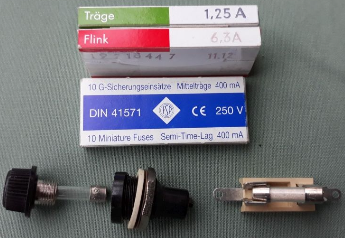
\includegraphics[width=0.85\textwidth]{foto/88}
    \caption{\scriptsize Feinsicherungen}
    \label{n_feinsicherungen}
\end{figure}

   \end{column}
\end{columns}

\end{frame}

\begin{frame}\begin{itemize}
  \item Nachdem eine Feinsicherung ausgelöst hat und man die Ursache behoben hat, muss man sie austauschen.
  \item Defekte Sicherungen dürfen \emph{nur durch gleichartige ersetzt werden}!
  \item Dabei ist sowohl auf \emph{Stromstärke} als auch die \emph{Auslösecharakteristik} zu achten, die angibt, wie schnell eine Sicherung auslöst (flink, mittelträge, träge).
  \end{itemize}
\end{frame}

\begin{frame}\begin{table}
\begin{DARCtabular}{ccc}
     Auslösecharakteristik  & Kennzeichen  & Abschaltzeit bei zehnfachem Nennstrom   \\
     flink  & F  & max. 30 ms  \\
     mittelträge  & MT  & max. 90 ms   \\
     träge  & T  & max. 300 ms   \\
\end{DARCtabular}
\caption{Kenngrößen von Feinsicherungen}
\label{n_feinsicherung}
\end{table}
\end{frame}

\begin{frame}
\only<1>{
\begin{QQuestion}{EK204}{Sie haben in ihren Kurzwellensender soeben einen Kurzschluss im Netzteil erfolgreich repariert. Durch den Fehler wurde auch die Feinsicherung für die Stromversorgung mit der Aufschrift \qty{20}{\A} \glqq Flink\grqq{} zerstört. Beim Austausch dieser Sicherung~...}{darf der Stromwert auch größer als \qty{20}{\A} sein, es muß jedoch eine Sicherung mit Auslösecharakteristik \glqq Flink\grqq{} eingesetzt werden.}
{darf bei gleichem Stromwert auch eine Sicherung mit Auslösecharakteristik \glqq Mittelträge\grqq{} oder \glqq Träge\grqq{} eingesetzt werden.}
{sollte eine Sicherung gleichen Stromwertes und gleicher Auslösecharakteristik eingesetzt werden.}
{kann ersatzweise auch eine Drahtbrücke aus dünnem Kupferdraht eingesetzt werden.}
\end{QQuestion}

}
\only<2>{
\begin{QQuestion}{EK204}{Sie haben in ihren Kurzwellensender soeben einen Kurzschluss im Netzteil erfolgreich repariert. Durch den Fehler wurde auch die Feinsicherung für die Stromversorgung mit der Aufschrift \qty{20}{\A} \glqq Flink\grqq{} zerstört. Beim Austausch dieser Sicherung~...}{darf der Stromwert auch größer als \qty{20}{\A} sein, es muß jedoch eine Sicherung mit Auslösecharakteristik \glqq Flink\grqq{} eingesetzt werden.}
{darf bei gleichem Stromwert auch eine Sicherung mit Auslösecharakteristik \glqq Mittelträge\grqq{} oder \glqq Träge\grqq{} eingesetzt werden.}
{\textbf{\textcolor{DARCgreen}{sollte eine Sicherung gleichen Stromwertes und gleicher Auslösecharakteristik eingesetzt werden.}}}
{kann ersatzweise auch eine Drahtbrücke aus dünnem Kupferdraht eingesetzt werden.}
\end{QQuestion}

}
\end{frame}%ENDCONTENT


\title{DARC Amateurfunklehrgang Klasse NEA}
\author{Grundlegende Schaltungen}
\institute{Deutscher Amateur Radio Club e.\,V.}
\begin{frame}
\maketitle
\end{frame}

\section{Schwingkreis I}
\label{section:schwingkreis_1}
\begin{frame}%STARTCONTENT
\begin{itemize}
  \item Kondensatoren und Spulen haben frequenzabhängige Widerstände
  \item Damit sind passive Filterschaltungen möglich, um nur bestimmte Frequenzen passieren zu lassen
  \end{itemize}
    \pause
    \emph{Zur Erinnerung}

\begin{itemize}
  \item Kondensator blockiert niedrige Frequenzen und  lässt hohe Frequenzen durch
  \item Spule blockiert hohe Frequenzen und lässt niedrige Frequenzen durch
  \end{itemize}


\end{frame}

\begin{frame}
\frametitle{Hochpass}
\begin{columns}
    \begin{column}{0.48\textwidth}
    \begin{itemize}
  \item Bei niedrigen Frequenzen hat der Kondensator einen sehr hohen Widerstand
  \item Schaltung wirkt wie ein frequenzabhängiger Spannungsteiler
  \item U<sub>A</sub> ist dadurch sehr klein
  \end{itemize}

    \end{column}
   \begin{column}{0.48\textwidth}
       
\begin{figure}
    \DARCimage{0.85\linewidth}{592include}
    \caption{\scriptsize Filtercharakteristik eines Hochpass}
    \label{e_hochpass}
\end{figure}


\begin{figure}
    \DARCimage{0.85\linewidth}{195include}
    \caption{\scriptsize Hochpass aus Kondensator und Widerstand}
    \label{e_hochpass_rc}
\end{figure}


   \end{column}
\end{columns}

\end{frame}

\begin{frame}
\only<1>{
\begin{PQuestion}{ED202}{Wie wird die dargestellte Filtercharakteristik bezeichnet?}{Bandsperre}
{Tiefpass}
{Bandpass}
{Hochpass}
{\DARCimage{0.75\linewidth}{592include}}\end{PQuestion}

}
\only<2>{
\begin{PQuestion}{ED202}{Wie wird die dargestellte Filtercharakteristik bezeichnet?}{Bandsperre}
{Tiefpass}
{Bandpass}
{\textbf{\textcolor{DARCgreen}{Hochpass}}}
{\DARCimage{0.75\linewidth}{592include}}\end{PQuestion}

}
\end{frame}

\begin{frame}
\only<1>{
\begin{PQuestion}{ED211}{Was stellt die folgende Schaltung dar? }{Hochpass}
{Sperrkreis}
{Bandpass}
{Tiefpass}
{\DARCimage{1.0\linewidth}{195include}}\end{PQuestion}

}
\only<2>{
\begin{PQuestion}{ED211}{Was stellt die folgende Schaltung dar? }{\textbf{\textcolor{DARCgreen}{Hochpass}}}
{Sperrkreis}
{Bandpass}
{Tiefpass}
{\DARCimage{1.0\linewidth}{195include}}\end{PQuestion}

}
\end{frame}

\begin{frame}
\only<1>{
\begin{PQuestion}{ED212}{Was stellt die folgende Schaltung dar? }{Hochpass}
{Sperrkreis}
{Bandpass}
{Tiefpass}
{\DARCimage{1.0\linewidth}{754include}}\end{PQuestion}

}
\only<2>{
\begin{PQuestion}{ED212}{Was stellt die folgende Schaltung dar? }{\textbf{\textcolor{DARCgreen}{Hochpass}}}
{Sperrkreis}
{Bandpass}
{Tiefpass}
{\DARCimage{1.0\linewidth}{754include}}\end{PQuestion}

}

\end{frame}

\begin{frame}
\only<1>{
\begin{question2x2}{ED213}{Welche Schaltung stellt ein Hochpassfilter dar?}{\DARCimage{1.0\linewidth}{182include}}
{\DARCimage{1.0\linewidth}{167include}}
{\DARCimage{1.0\linewidth}{172include}}
{\DARCimage{1.0\linewidth}{165include}}
\end{question2x2}

}
\only<2>{
\begin{question2x2}{ED213}{Welche Schaltung stellt ein Hochpassfilter dar?}{\DARCimage{1.0\linewidth}{182include}}
{\DARCimage{1.0\linewidth}{167include}}
{\DARCimage{1.0\linewidth}{172include}}
{\textbf{\textcolor{DARCgreen}{\DARCimage{1.0\linewidth}{165include}}}}
\end{question2x2}

}

\end{frame}

\begin{frame}
\frametitle{Tiefpass}
\begin{columns}
    \begin{column}{0.48\textwidth}
    \begin{itemize}
  \item Bei niedrigen Frequenzen hat der Kondensator einen sehr hohen Widerstand
  \item Schaltung wirkt wie ein frequenzabhängiger Spannungsteiler
  \item U<sub>A</sub> ist dadurch sehr groß
  \end{itemize}

    \end{column}
   \begin{column}{0.48\textwidth}
       
\begin{figure}
    \DARCimage{0.85\linewidth}{591include}
    \caption{\scriptsize Filtercharakteristik eines Tiefpass}
    \label{e_hochpass}
\end{figure}


\begin{figure}
    \DARCimage{0.85\linewidth}{175include}
    \caption{\scriptsize Tiefpass aus Kondensator und Widerstand}
    \label{e_tiefpass_rc}
\end{figure}


   \end{column}
\end{columns}

\end{frame}

\begin{frame}
\only<1>{
\begin{PQuestion}{ED201}{Wie wird die dargestellte Filtercharakteristik bezeichnet?}{Bandsperre}
{Hochpass}
{Bandpass}
{Tiefpass}
{\DARCimage{0.75\linewidth}{591include}}\end{PQuestion}

}
\only<2>{
\begin{PQuestion}{ED201}{Wie wird die dargestellte Filtercharakteristik bezeichnet?}{Bandsperre}
{Hochpass}
{Bandpass}
{\textbf{\textcolor{DARCgreen}{Tiefpass}}}
{\DARCimage{0.75\linewidth}{591include}}\end{PQuestion}

}
\end{frame}

\begin{frame}
\only<1>{
\begin{PQuestion}{ED208}{Was stellt die folgende Schaltung dar? }{Bandpass}
{Sperrkreis}
{Tiefpass}
{Hochpass}
{\DARCimage{1.0\linewidth}{175include}}\end{PQuestion}

}
\only<2>{
\begin{PQuestion}{ED208}{Was stellt die folgende Schaltung dar? }{Bandpass}
{Sperrkreis}
{\textbf{\textcolor{DARCgreen}{Tiefpass}}}
{Hochpass}
{\DARCimage{1.0\linewidth}{175include}}\end{PQuestion}

}
\end{frame}

\begin{frame}
\only<1>{
\begin{PQuestion}{ED209}{Was stellt die folgende Schaltung dar? }{Tiefpass}
{Sperrkreis}
{Bandpass}
{Hochpass}
{\DARCimage{1.0\linewidth}{756include}}\end{PQuestion}

}
\only<2>{
\begin{PQuestion}{ED209}{Was stellt die folgende Schaltung dar? }{\textbf{\textcolor{DARCgreen}{Tiefpass}}}
{Sperrkreis}
{Bandpass}
{Hochpass}
{\DARCimage{1.0\linewidth}{756include}}\end{PQuestion}

}

\end{frame}

\begin{frame}
\only<1>{
\begin{question2x2}{ED210}{Welche Schaltung könnte für die Tiefpassfilterung in einem Mikrofonverstärker eingesetzt werden?}{\DARCimage{1.0\linewidth}{170include}}
{\DARCimage{1.0\linewidth}{173include}}
{\DARCimage{1.0\linewidth}{161include}}
{\DARCimage{1.0\linewidth}{169include}}
\end{question2x2}

}
\only<2>{
\begin{question2x2}{ED210}{Welche Schaltung könnte für die Tiefpassfilterung in einem Mikrofonverstärker eingesetzt werden?}{\textbf{\textcolor{DARCgreen}{\DARCimage{1.0\linewidth}{170include}}}}
{\DARCimage{1.0\linewidth}{173include}}
{\DARCimage{1.0\linewidth}{161include}}
{\DARCimage{1.0\linewidth}{169include}}
\end{question2x2}

}

\end{frame}

\begin{frame}
\frametitle{Serienschwingkreis}
\begin{columns}
    \begin{column}{0.48\textwidth}
    \begin{itemize}
  \item Es gibt eine Resonanzfrequenz, bei der der Wechselstromwiderstand (Impedanz) sehr gering ist
  \item Bandpass, Saugkreis (eine Frequenz wird rausgesaugt)
  \end{itemize}

    \end{column}
   \begin{column}{0.48\textwidth}
       
\begin{figure}
    \DARCimage{0.85\linewidth}{189include}
    \caption{\scriptsize Impedanzverlauf eines Serienschwingkreis}
    \label{e_serienschwingkreis_z}
\end{figure}


\begin{figure}
    \DARCimage{0.85\linewidth}{757include}
    \caption{\scriptsize Serienschwingkreis aus Kondensator und Spule}
    \label{e_serienschwingkreis_cl}
\end{figure}


   \end{column}
\end{columns}

\end{frame}%ENDCONTENT


\section{Schwingkreis II}
\label{section:schwingkreis_2}
\begin{frame}%STARTCONTENT

\only<1>{
\begin{PQuestion}{AD201}{Welche Grenzfrequenz ergibt sich bei einem Hochpass mit einem Widerstand von \qty{4,7}{\kohm} und einem Kondensator von \qty{2,2}{\nF}?}{\qty{154}{\Hz}}
{\qty{1,54}{\kHz}}
{\qty{154}{\kHz}}
{\qty{15,4}{\kHz}}
{\DARCimage{1.0\linewidth}{195include}}\end{PQuestion}

}
\only<2>{
\begin{PQuestion}{AD201}{Welche Grenzfrequenz ergibt sich bei einem Hochpass mit einem Widerstand von \qty{4,7}{\kohm} und einem Kondensator von \qty{2,2}{\nF}?}{\qty{154}{\Hz}}
{\qty{1,54}{\kHz}}
{\qty{154}{\kHz}}
{\textbf{\textcolor{DARCgreen}{\qty{15,4}{\kHz}}}}
{\DARCimage{1.0\linewidth}{195include}}\end{PQuestion}

}
\end{frame}

\begin{frame}
\frametitle{Lösungsweg}
\begin{itemize}
  \item gegeben: $R = 4,7kΩ$
  \item gegeben: $C = 2,2nF$
  \item gesucht: $f_g$
  \end{itemize}
    \pause
    $f_g = \frac{1}{2 \cdot \pi \cdot R \cdot C} = \frac{1}{2 \cdot \pi \cdot 4,7kΩ \cdot 2,2nF} = 15,4kHz$



\end{frame}

\begin{frame}
\only<1>{
\begin{PQuestion}{AD202}{Welche Grenzfrequenz ergibt sich bei einem Tiefpass mit einem Widerstand von \qty{10}{\kohm} und einem Kondensator von \qty{47}{\nF}?}{\qty{339}{\kHz}}
{\qty{3,39}{\kHz}}
{\qty{339}{\Hz}}
{\qty{33,9}{\Hz}}
{\DARCimage{1.0\linewidth}{175include}}\end{PQuestion}

}
\only<2>{
\begin{PQuestion}{AD202}{Welche Grenzfrequenz ergibt sich bei einem Tiefpass mit einem Widerstand von \qty{10}{\kohm} und einem Kondensator von \qty{47}{\nF}?}{\qty{339}{\kHz}}
{\qty{3,39}{\kHz}}
{\textbf{\textcolor{DARCgreen}{\qty{339}{\Hz}}}}
{\qty{33,9}{\Hz}}
{\DARCimage{1.0\linewidth}{175include}}\end{PQuestion}

}
\end{frame}

\begin{frame}
\frametitle{Lösungsweg}
\begin{itemize}
  \item gegeben: $R = 10kΩ$
  \item gegeben: $C = 47nF$
  \item gesucht: $f_g$
  \end{itemize}
    \pause
    $f_g = \frac{1}{2 \cdot \pi \cdot R \cdot C} = \frac{1}{2 \cdot \pi \cdot 10kΩ \cdot 47nF} = 339Hz$



\end{frame}

\begin{frame}
\only<1>{
\begin{PQuestion}{AD203}{Wo liegt die Grenzfrequenz des Audio-Verstärkers, wenn $R_{1}$ = \qty{4,7}{\kilo\ohm}, $C_1$ = \qty{6,8}{\nF} und $C_2$ = \qty{47}{\nF} betragen? Der Verstärker hat eine Grenzfrequenz von \qty{1}{\MHz} und die Impedanz des Eingangs PIN 2 ist mit \qty{1}{\Mohm} sehr hochohmig.}{ca. 5~kHz}
{ca. 720~Hz}
{ca. 2,7~kHz}
{ca. 294~Hz}
{\DARCimage{1.0\linewidth}{488include}}\end{PQuestion}

}
\only<2>{
\begin{PQuestion}{AD203}{Wo liegt die Grenzfrequenz des Audio-Verstärkers, wenn $R_{1}$ = \qty{4,7}{\kilo\ohm}, $C_1$ = \qty{6,8}{\nF} und $C_2$ = \qty{47}{\nF} betragen? Der Verstärker hat eine Grenzfrequenz von \qty{1}{\MHz} und die Impedanz des Eingangs PIN 2 ist mit \qty{1}{\Mohm} sehr hochohmig.}{\textbf{\textcolor{DARCgreen}{ca. 5~kHz}}}
{ca. 720~Hz}
{ca. 2,7~kHz}
{ca. 294~Hz}
{\DARCimage{1.0\linewidth}{488include}}\end{PQuestion}

}
\end{frame}

\begin{frame}
\frametitle{Lösungsweg}
\begin{itemize}
  \item gegeben: $R_1 = 4,7kΩ$
  \item gegeben: $C_1 = 6,8nF$
  \item gesucht: $f_g$
  \end{itemize}
    \pause
    $C_2$ und alle weiteren Angaben sind für den Tiefpass uninteressant.
    \pause
    $f_g = \frac{1}{2 \cdot \pi \cdot R_1 \cdot C_1} = \frac{1}{2 \cdot \pi \cdot 4,7kΩ \cdot 6,8nF} \approx 5kHz$



\end{frame}

\begin{frame}
\only<1>{
\begin{QQuestion}{AD206}{Was ist im Resonanzfall bei der Reihenschaltung einer Induktivität mit einer Kapazität erfüllt?}{Der Betrag des elektrischen Feldes in der Spule ist dann gleich dem Betrag des elektrischen Feldes im Kondensator.}
{Der Betrag des Verlustwiderstandes der Spule ist dann gleich dem Betrag des Verlustwiderstandes des Kondensators.}
{Der Betrag des induktiven Widerstands ist dann gleich dem Betrag des kapazitiven Widerstands.}
{Der Betrag des magnetischen Feldes in der Spule ist dann gleich dem Betrag des magnetischen Feldes im Kondensator.}
\end{QQuestion}

}
\only<2>{
\begin{QQuestion}{AD206}{Was ist im Resonanzfall bei der Reihenschaltung einer Induktivität mit einer Kapazität erfüllt?}{Der Betrag des elektrischen Feldes in der Spule ist dann gleich dem Betrag des elektrischen Feldes im Kondensator.}
{Der Betrag des Verlustwiderstandes der Spule ist dann gleich dem Betrag des Verlustwiderstandes des Kondensators.}
{\textbf{\textcolor{DARCgreen}{Der Betrag des induktiven Widerstands ist dann gleich dem Betrag des kapazitiven Widerstands.}}}
{Der Betrag des magnetischen Feldes in der Spule ist dann gleich dem Betrag des magnetischen Feldes im Kondensator.}
\end{QQuestion}

}
\end{frame}

\begin{frame}
\only<1>{
\begin{PQuestion}{AD207}{Bei der Resonanzfrequenz ist die Impedanz dieser Schaltung~...}{gleich dem Wirkwiderstand $R$.}
{unendlich hoch.}
{gleich dem kapazitiven Widerstand $X_{\symup{C}}$.}
{gleich dem induktiven Widerstand $X_{\symup{L}}$.}
{\DARCimage{1.0\linewidth}{181include}}\end{PQuestion}

}
\only<2>{
\begin{PQuestion}{AD207}{Bei der Resonanzfrequenz ist die Impedanz dieser Schaltung~...}{\textbf{\textcolor{DARCgreen}{gleich dem Wirkwiderstand $R$.}}}
{unendlich hoch.}
{gleich dem kapazitiven Widerstand $X_{\symup{C}}$.}
{gleich dem induktiven Widerstand $X_{\symup{L}}$.}
{\DARCimage{1.0\linewidth}{181include}}\end{PQuestion}

}
\end{frame}

\begin{frame}
\only<1>{
\begin{question2x2}{AD204}{Welcher Schwingkreis passt zu dem neben der jeweiligen Schaltung dargestellten Verlauf der Impedanz?}{\DARCimage{1.0\linewidth}{230include}}
{\DARCimage{1.0\linewidth}{231include}}
{\DARCimage{1.0\linewidth}{232include}}
{\DARCimage{1.0\linewidth}{826include}}
\end{question2x2}

}
\only<2>{
\begin{question2x2}{AD204}{Welcher Schwingkreis passt zu dem neben der jeweiligen Schaltung dargestellten Verlauf der Impedanz?}{\textbf{\textcolor{DARCgreen}{\DARCimage{1.0\linewidth}{230include}}}}
{\DARCimage{1.0\linewidth}{231include}}
{\DARCimage{1.0\linewidth}{232include}}
{\DARCimage{1.0\linewidth}{826include}}
\end{question2x2}

}
\end{frame}

\begin{frame}
\only<1>{
\begin{PQuestion}{AD208}{Welche Resonanzfrequenz $f_{\symup{res}}$ hat die Reihenschaltung einer Spule von \qty{1,2}{\micro\H} mit einem Kondensator von \qty{6,8}{\pF} und einem Widerstand von \qty{10}{\ohm}?}{\qty{55,7}{\MHz}}
{\qty{5,57}{\MHz}}
{\qty{557}{\MHz}}
{\qty{557}{\kHz}}
{\DARCimage{1.0\linewidth}{181include}}\end{PQuestion}

}
\only<2>{
\begin{PQuestion}{AD208}{Welche Resonanzfrequenz $f_{\symup{res}}$ hat die Reihenschaltung einer Spule von \qty{1,2}{\micro\H} mit einem Kondensator von \qty{6,8}{\pF} und einem Widerstand von \qty{10}{\ohm}?}{\textbf{\textcolor{DARCgreen}{\qty{55,7}{\MHz}}}}
{\qty{5,57}{\MHz}}
{\qty{557}{\MHz}}
{\qty{557}{\kHz}}
{\DARCimage{1.0\linewidth}{181include}}\end{PQuestion}

}
\end{frame}

\begin{frame}
\frametitle{Lösungsweg}
\begin{itemize}
  \item gegeben: $L = 1,2µH$
  \item gegeben: $C = 6,8pF$
  \item gegeben: $R = 10Ω$
  \item gesucht: $f_0$
  \end{itemize}
    \pause
    $f_0 = \frac{1}{2 \cdot \pi \cdot \sqrt{L \cdot C}} = \frac{1}{2 \cdot \pi \cdot \sqrt{1,2µH \cdot 6,8pF}} = 55,7MHz$
    \pause
    Widerstand $R$ wird zur Berechnung nicht benötigt.



\end{frame}

\begin{frame}
\only<1>{
\begin{PQuestion}{AD209}{Welche Resonanzfrequenz $f_{\symup{res}}$ hat die Reihenschaltung einer Spule von \qty{10}{\micro\H} mit einem Kondensator von \qty{1}{\nF} und einem Widerstand von \qty{0,1}{\kohm}?}{\qty{15,92}{\MHz}}
{\qty{159,2}{\kHz}}
{\qty{1,592}{\MHz}}
{\qty{15,92}{\kHz}}
{\DARCimage{1.0\linewidth}{181include}}\end{PQuestion}

}
\only<2>{
\begin{PQuestion}{AD209}{Welche Resonanzfrequenz $f_{\symup{res}}$ hat die Reihenschaltung einer Spule von \qty{10}{\micro\H} mit einem Kondensator von \qty{1}{\nF} und einem Widerstand von \qty{0,1}{\kohm}?}{\qty{15,92}{\MHz}}
{\qty{159,2}{\kHz}}
{\textbf{\textcolor{DARCgreen}{\qty{1,592}{\MHz}}}}
{\qty{15,92}{\kHz}}
{\DARCimage{1.0\linewidth}{181include}}\end{PQuestion}

}
\end{frame}

\begin{frame}
\frametitle{Lösungsweg}
\begin{itemize}
  \item gegeben: $L = 10µH$
  \item gegeben: $C = 1nF$
  \item gesucht: $f_0$
  \end{itemize}
    \pause
    $f_0 = \frac{1}{2 \cdot \pi \cdot \sqrt{L \cdot C}} = \frac{1}{2 \cdot \pi \cdot \sqrt{10µH \cdot 1nF}} = 1,592MHz$



\end{frame}

\begin{frame}
\only<1>{
\begin{PQuestion}{AD210}{Welche Resonanzfrequenz $f_{\symup{res}}$ hat die Reihenschaltung einer Spule von \qty{100}{\micro\H} mit einem Kondensator von \qty{0,01}{\micro\F} und einem Widerstand von \qty{100}{\ohm}?}{\qty{1,59}{\kHz}}
{\qty{15,9}{\kHz}}
{\qty{159}{\kHz}}
{\qty{1590}{\kHz}}
{\DARCimage{1.0\linewidth}{181include}}\end{PQuestion}

}
\only<2>{
\begin{PQuestion}{AD210}{Welche Resonanzfrequenz $f_{\symup{res}}$ hat die Reihenschaltung einer Spule von \qty{100}{\micro\H} mit einem Kondensator von \qty{0,01}{\micro\F} und einem Widerstand von \qty{100}{\ohm}?}{\qty{1,59}{\kHz}}
{\qty{15,9}{\kHz}}
{\textbf{\textcolor{DARCgreen}{\qty{159}{\kHz}}}}
{\qty{1590}{\kHz}}
{\DARCimage{1.0\linewidth}{181include}}\end{PQuestion}

}
\end{frame}

\begin{frame}
\frametitle{Lösungsweg}
\begin{itemize}
  \item gegeben: $L = 100µH$
  \item gegeben: $C = 0,01µF$
  \item gesucht: $f_0$
  \end{itemize}
    \pause
    $f_0 = \frac{1}{2 \cdot \pi \cdot \sqrt{L \cdot C}} = \frac{1}{2 \cdot \pi \cdot \sqrt{100µH \cdot 0,01µF}} = 159kHz$



\end{frame}

\begin{frame}
\only<1>{
\begin{PQuestion}{AD211}{Welche Resonanzfrequenz $f_{\symup{res}}$ hat die Parallelschaltung einer Spule von \qty{2,2}{\micro\H} mit einem Kondensator von \qty{56}{\pF} und einem Widerstand von \qty{10}{\kohm}?}{\qty{14,34}{\MHz}}
{\qty{143,4}{\MHz}}
{\qty{1,434}{\MHz}}
{\qty{143,4}{\kHz}}
{\DARCimage{1.0\linewidth}{233include}}\end{PQuestion}

}
\only<2>{
\begin{PQuestion}{AD211}{Welche Resonanzfrequenz $f_{\symup{res}}$ hat die Parallelschaltung einer Spule von \qty{2,2}{\micro\H} mit einem Kondensator von \qty{56}{\pF} und einem Widerstand von \qty{10}{\kohm}?}{\textbf{\textcolor{DARCgreen}{\qty{14,34}{\MHz}}}}
{\qty{143,4}{\MHz}}
{\qty{1,434}{\MHz}}
{\qty{143,4}{\kHz}}
{\DARCimage{1.0\linewidth}{233include}}\end{PQuestion}

}
\end{frame}

\begin{frame}
\frametitle{Lösungsweg}
\begin{itemize}
  \item gegeben: $L = 2,2µH$
  \item gegeben: $C = 56pF$
  \item gesucht: $f_0$
  \end{itemize}
    \pause
    $f_0 = \frac{1}{2 \cdot \pi \cdot \sqrt{L \cdot C}} = \frac{1}{2 \cdot \pi \cdot \sqrt{2,2µH \cdot 56pF}} = 14,34MHz$



\end{frame}

\begin{frame}
\only<1>{
\begin{PQuestion}{AD212}{Wie groß ist die Resonanzfrequenz dieser Schaltung, wenn die Kapazitäten $C_1$ = \qty{0,1}{\nF}, $C_2$ = \qty{1,5}{\nF}, $C_3$ = \qty{220}{\pF} und die Induktivität der Spule \qty{1,2}{\mH} betragen?}{\qty{10,77}{\kHz}}
{\qty{107,7}{\kHz}}
{\qty{1,077}{\kHz}}
{\qty{1,077}{\MHz}}
{\DARCimage{1.0\linewidth}{776include}}\end{PQuestion}

}
\only<2>{
\begin{PQuestion}{AD212}{Wie groß ist die Resonanzfrequenz dieser Schaltung, wenn die Kapazitäten $C_1$ = \qty{0,1}{\nF}, $C_2$ = \qty{1,5}{\nF}, $C_3$ = \qty{220}{\pF} und die Induktivität der Spule \qty{1,2}{\mH} betragen?}{\qty{10,77}{\kHz}}
{\textbf{\textcolor{DARCgreen}{\qty{107,7}{\kHz}}}}
{\qty{1,077}{\kHz}}
{\qty{1,077}{\MHz}}
{\DARCimage{1.0\linewidth}{776include}}\end{PQuestion}

}
\end{frame}

\begin{frame}
\frametitle{Lösungsweg}
\begin{itemize}
  \item gegeben: $C_1 = 0,1nF$
  \item gegeben: $C_2 = 1,5nF$
  \item gegeben: $C_3 = 220pF$
  \item gegeben: $L = 1,2mH$
  \item gesucht: $f_0$
  \end{itemize}
    \pause
    $C = C_1 + C_2 + C_3 = 0,1nF + 1,5nF + 220pF = 1,82nF$
    \pause
    $f_0 = \frac{1}{2 \cdot \pi \cdot \sqrt{L \cdot C}} = \frac{1}{2 \cdot \pi \cdot \sqrt{1,2mH \cdot 1,82nF}} = 107,7kHz$



\end{frame}

\begin{frame}
\only<1>{
\begin{QQuestion}{AD213}{Sie wollen die Resonanzfrequenz eines Schwingkreises vergrößern. Welche der folgenden Maßnahmen ist geeignet?}{Kleineren Spulenwert verwenden}
{Spule zusammenschieben}
{Ferritkern in die Spule einführen}
{Anzahl der Spulenwindungen erhöhen}
\end{QQuestion}

}
\only<2>{
\begin{QQuestion}{AD213}{Sie wollen die Resonanzfrequenz eines Schwingkreises vergrößern. Welche der folgenden Maßnahmen ist geeignet?}{\textbf{\textcolor{DARCgreen}{Kleineren Spulenwert verwenden}}}
{Spule zusammenschieben}
{Ferritkern in die Spule einführen}
{Anzahl der Spulenwindungen erhöhen}
\end{QQuestion}

}
\end{frame}

\begin{frame}
\only<1>{
\begin{QQuestion}{AD214}{Sie wollen die Resonanzfrequenz eines Schwingkreises vergrößern. Welche der folgenden Maßnahmen ist geeignet?}{Spule zusammenschieben}
{Anzahl der Spulenwindungen verringern}
{Größeren Spulenwert verwenden}
{Größeren Kondensatorwert verwenden}
\end{QQuestion}

}
\only<2>{
\begin{QQuestion}{AD214}{Sie wollen die Resonanzfrequenz eines Schwingkreises vergrößern. Welche der folgenden Maßnahmen ist geeignet?}{Spule zusammenschieben}
{\textbf{\textcolor{DARCgreen}{Anzahl der Spulenwindungen verringern}}}
{Größeren Spulenwert verwenden}
{Größeren Kondensatorwert verwenden}
\end{QQuestion}

}
\end{frame}

\begin{frame}
\only<1>{
\begin{QQuestion}{AD215}{Sie wollen die Resonanzfrequenz eines Schwingkreises verringern. Welche der folgenden Maßnahmen ist geeignet?}{Anzahl der Spulenwindungen verringern}
{Kleineren Spulenwert verwenden}
{Größeren Kondensatorwert verwenden}
{Spule auseinanderziehen}
\end{QQuestion}

}
\only<2>{
\begin{QQuestion}{AD215}{Sie wollen die Resonanzfrequenz eines Schwingkreises verringern. Welche der folgenden Maßnahmen ist geeignet?}{Anzahl der Spulenwindungen verringern}
{Kleineren Spulenwert verwenden}
{\textbf{\textcolor{DARCgreen}{Größeren Kondensatorwert verwenden}}}
{Spule auseinanderziehen}
\end{QQuestion}

}
\end{frame}

\begin{frame}
\only<1>{
\begin{QQuestion}{AD216}{Sie wollen die Resonanzfrequenz eines Schwingkreises verringern. Welche der folgenden Maßnahmen ist geeignet?}{Kleineren Spulenwert verwenden}
{Spule auseinanderziehen}
{Kleineren Kondensatorwert verwenden}
{Spule zusammenschieben}
\end{QQuestion}

}
\only<2>{
\begin{QQuestion}{AD216}{Sie wollen die Resonanzfrequenz eines Schwingkreises verringern. Welche der folgenden Maßnahmen ist geeignet?}{Kleineren Spulenwert verwenden}
{Spule auseinanderziehen}
{Kleineren Kondensatorwert verwenden}
{\textbf{\textcolor{DARCgreen}{Spule zusammenschieben}}}
\end{QQuestion}

}
\end{frame}

\begin{frame}
\only<1>{
\begin{QQuestion}{AD217}{Sie wollen die Resonanzfrequenz eines Schwingkreises verringern. Welche der folgenden Maßnahmen ist geeignet?}{Kleineren Spulenwert verwenden}
{Spule auseinanderziehen}
{Kleineren Kondensatorwert verwenden}
{Ferritkern in die Spule einführen}
\end{QQuestion}

}
\only<2>{
\begin{QQuestion}{AD217}{Sie wollen die Resonanzfrequenz eines Schwingkreises verringern. Welche der folgenden Maßnahmen ist geeignet?}{Kleineren Spulenwert verwenden}
{Spule auseinanderziehen}
{Kleineren Kondensatorwert verwenden}
{\textbf{\textcolor{DARCgreen}{Ferritkern in die Spule einführen}}}
\end{QQuestion}

}
\end{frame}

\begin{frame}
\only<1>{
\begin{PQuestion}{AD218}{Wie verändert sich die Frequenz des Schwingkreises in der folgenden Schaltung, wenn das Potentiometer mehr in Richtung X gedreht wird?}{Die Frequenz des Schwingkreises ändert sich nicht.}
{Die Frequenz des Schwingkreises sinkt.}
{Die Frequenz des Schwingkreises steigt.}
{Die Frequenz sinkt zunächst und steigt dann stark an.}
{\DARCimage{1.0\linewidth}{752include}}\end{PQuestion}

}
\only<2>{
\begin{PQuestion}{AD218}{Wie verändert sich die Frequenz des Schwingkreises in der folgenden Schaltung, wenn das Potentiometer mehr in Richtung X gedreht wird?}{Die Frequenz des Schwingkreises ändert sich nicht.}
{Die Frequenz des Schwingkreises sinkt.}
{\textbf{\textcolor{DARCgreen}{Die Frequenz des Schwingkreises steigt.}}}
{Die Frequenz sinkt zunächst und steigt dann stark an.}
{\DARCimage{1.0\linewidth}{752include}}\end{PQuestion}

}
\end{frame}

\begin{frame}
\only<1>{
\begin{PQuestion}{AD205}{Welche der nachfolgenden Beschreibungen trifft auf diese Schaltung zu und wie nennt man sie? }{Es handelt sich um eine Bandsperre. Frequenzen oberhalb der oberen Grenzfrequenz und Frequenzen unterhalb der unteren Grenzfrequenz werden durchgelassen. Sie bedämpft nur einen bestimmten Frequenzbereich.}
{Es handelt sich um einen Hochpass. Frequenzen unterhalb der Grenzfrequenz werden bedämpft, oberhalb der Grenzfrequenz durchgelassen.}
{Es handelt sich um einen Tiefpass. Frequenzen oberhalb der Grenzfrequenz werden bedämpft, unterhalb der Grenzfrequenz durchgelassen.}
{Es handelt sich um einen Bandpass. Frequenzen oberhalb der oberen Grenzfrequenz und Frequenzen unterhalb der unteren Grenzfrequenz werden bedämpft. Er lässt nur einen bestimmten Frequenzbereich passieren.}
{\DARCimage{1.0\linewidth}{785include}}\end{PQuestion}

}
\only<2>{
\begin{PQuestion}{AD205}{Welche der nachfolgenden Beschreibungen trifft auf diese Schaltung zu und wie nennt man sie? }{Es handelt sich um eine Bandsperre. Frequenzen oberhalb der oberen Grenzfrequenz und Frequenzen unterhalb der unteren Grenzfrequenz werden durchgelassen. Sie bedämpft nur einen bestimmten Frequenzbereich.}
{Es handelt sich um einen Hochpass. Frequenzen unterhalb der Grenzfrequenz werden bedämpft, oberhalb der Grenzfrequenz durchgelassen.}
{Es handelt sich um einen Tiefpass. Frequenzen oberhalb der Grenzfrequenz werden bedämpft, unterhalb der Grenzfrequenz durchgelassen.}
{\textbf{\textcolor{DARCgreen}{Es handelt sich um einen Bandpass. Frequenzen oberhalb der oberen Grenzfrequenz und Frequenzen unterhalb der unteren Grenzfrequenz werden bedämpft. Er lässt nur einen bestimmten Frequenzbereich passieren.}}}
{\DARCimage{1.0\linewidth}{785include}}\end{PQuestion}

}
\end{frame}

\begin{frame}
\only<1>{
\begin{PQuestion}{AD219}{Wie groß ist die Bandbreite in dem dargestellten Diagramm bei \qty{-60}{\decibel}?}{Etwa \qty{6,0}{\kHz}}
{Etwa \qty{6,5}{\kHz}}
{Etwa \qty{4,0}{\kHz}}
{Etwa \qty{2,5}{\kHz}}
{\DARCimage{1.0\linewidth}{38include}}\end{PQuestion}

}
\only<2>{
\begin{PQuestion}{AD219}{Wie groß ist die Bandbreite in dem dargestellten Diagramm bei \qty{-60}{\decibel}?}{Etwa \qty{6,0}{\kHz}}
{Etwa \qty{6,5}{\kHz}}
{\textbf{\textcolor{DARCgreen}{Etwa \qty{4,0}{\kHz}}}}
{Etwa \qty{2,5}{\kHz}}
{\DARCimage{1.0\linewidth}{38include}}\end{PQuestion}

}
\end{frame}

\begin{frame}
\only<1>{
\begin{QQuestion}{AD221}{Ein Quarzfilter mit einer \qty{3}{\decibel}-Bandbreite von \qty{2,7}{\kHz} eignet sich besonders zur Verwendung in einem Sendeempfänger für~...}{FM.}
{AM.}
{SSB.}
{CW.}
\end{QQuestion}

}
\only<2>{
\begin{QQuestion}{AD221}{Ein Quarzfilter mit einer \qty{3}{\decibel}-Bandbreite von \qty{2,7}{\kHz} eignet sich besonders zur Verwendung in einem Sendeempfänger für~...}{FM.}
{AM.}
{\textbf{\textcolor{DARCgreen}{SSB.}}}
{CW.}
\end{QQuestion}

}
\end{frame}

\begin{frame}
\only<1>{
\begin{QQuestion}{AD222}{Ein Quarzfilter mit einer \qty{3}{\decibel}-Bandbreite von \qty{500}{\Hz} eignet sich besonders zur Verwendung in einem Sendeempfänger für~...}{SSB.}
{CW.}
{AM.}
{FM.}
\end{QQuestion}

}
\only<2>{
\begin{QQuestion}{AD222}{Ein Quarzfilter mit einer \qty{3}{\decibel}-Bandbreite von \qty{500}{\Hz} eignet sich besonders zur Verwendung in einem Sendeempfänger für~...}{SSB.}
{\textbf{\textcolor{DARCgreen}{CW.}}}
{AM.}
{FM.}
\end{QQuestion}

}
\end{frame}

\begin{frame}
\only<1>{
\begin{QQuestion}{AD220}{Wie ergibt sich die Bandbreite $B$ eines Parallelschwingkreises aus der Resonanzkurve?}{Die Bandbreite ergibt sich aus der Differenz der beiden Frequenzen, bei denen die Spannung auf den 0,7-fachen Wert gegenüber der maximalen Spannung bei der Resonanzfrequenz abgesunken ist.}
{Die Bandbreite ergibt sich aus der Differenz der beiden Frequenzen, bei denen die Spannung auf den 0,5-fachen Wert gegenüber der maximalen Spannung bei der Resonanzfrequenz abgesunken ist.}
{Die Bandbreite ergibt sich aus der Multiplikation der Resonanzfrequenz mit dem Faktor 0,5.}
{Die Bandbreite ergibt sich aus der Multiplikation der Resonanzfrequenz mit dem Faktor 0,7.}
\end{QQuestion}

}
\only<2>{
\begin{QQuestion}{AD220}{Wie ergibt sich die Bandbreite $B$ eines Parallelschwingkreises aus der Resonanzkurve?}{\textbf{\textcolor{DARCgreen}{Die Bandbreite ergibt sich aus der Differenz der beiden Frequenzen, bei denen die Spannung auf den 0,7-fachen Wert gegenüber der maximalen Spannung bei der Resonanzfrequenz abgesunken ist.}}}
{Die Bandbreite ergibt sich aus der Differenz der beiden Frequenzen, bei denen die Spannung auf den 0,5-fachen Wert gegenüber der maximalen Spannung bei der Resonanzfrequenz abgesunken ist.}
{Die Bandbreite ergibt sich aus der Multiplikation der Resonanzfrequenz mit dem Faktor 0,5.}
{Die Bandbreite ergibt sich aus der Multiplikation der Resonanzfrequenz mit dem Faktor 0,7.}
\end{QQuestion}

}
\end{frame}

\begin{frame}
\only<1>{
\begin{QQuestion}{AD223}{Welche Bandbreite $B$ hat die Reihenschaltung einer Spule von \qty{100}{\micro\H} mit einem Kondensator von \qty{0,01}{\micro\F} und einem Widerstand von \qty{10}{\ohm}?}{\qty{1,59}{\kHz}}
{\qty{159}{\kHz}}
{\qty{15,9}{\kHz}}
{\qty{159}{\Hz}}
\end{QQuestion}

}
\only<2>{
\begin{QQuestion}{AD223}{Welche Bandbreite $B$ hat die Reihenschaltung einer Spule von \qty{100}{\micro\H} mit einem Kondensator von \qty{0,01}{\micro\F} und einem Widerstand von \qty{10}{\ohm}?}{\qty{1,59}{\kHz}}
{\qty{159}{\kHz}}
{\textbf{\textcolor{DARCgreen}{\qty{15,9}{\kHz}}}}
{\qty{159}{\Hz}}
\end{QQuestion}

}
\end{frame}

\begin{frame}
\frametitle{Lösungsweg}
\begin{itemize}
  \item gegeben: $L = 100µH$
  \item gegeben: $C = 0,01µF$
  \item gegeben: $R_S = 10Ω$
  \item gesucht: $B$
  \end{itemize}
    \pause
    $B = \frac{R_S}{2\cdot \pi \cdot L} = \frac{10Ω}{2\cdot \pi \cdot 100µH} = 15,9kHz$



\end{frame}

\begin{frame}
\only<1>{
\begin{QQuestion}{AD225}{Welchen Gütefaktor $Q$ hat die Reihenschaltung einer Spule von \qty{100}{\micro\H} mit einem Kondensator von \qty{0,01}{\micro\F} und einem Widerstand von \qty{10}{\ohm}?}{10}
{1}
{0,1}
{100}
\end{QQuestion}

}
\only<2>{
\begin{QQuestion}{AD225}{Welchen Gütefaktor $Q$ hat die Reihenschaltung einer Spule von \qty{100}{\micro\H} mit einem Kondensator von \qty{0,01}{\micro\F} und einem Widerstand von \qty{10}{\ohm}?}{\textbf{\textcolor{DARCgreen}{10}}}
{1}
{0,1}
{100}
\end{QQuestion}

}
\end{frame}

\begin{frame}
\frametitle{Lösungsweg}
\begin{itemize}
  \item gegeben: $L = 100µH$
  \item gegeben: $C = 0,01µF$
  \item gegeben: $R_S = 10Ω$
  \item gesucht: $Q$
  \end{itemize}
    \pause
    $f_0 = \frac{1}{2 \cdot \pi \cdot \sqrt{L \cdot C}} = \frac{1}{2 \cdot \pi \cdot \sqrt{100µH \cdot 0,01µF}} = 159,2kHz$
    \pause
    $B$ oder $X_L$ ausrechnen – $B$ haben wir schon vorher ausgerechnet

$B = \frac{R_S}{2\cdot \pi \cdot L} = \frac{10Ω}{2\cdot \pi \cdot 100µH} = 15,92kHz$
    \pause
    $Q = \frac{f_0}{B} = \frac{159,2kHz}{15,92kHz} = 10$



\end{frame}

\begin{frame}
\only<1>{
\begin{QQuestion}{AD224}{Welche Bandbreite $B$ hat die Parallelschaltung einer Spule von \qty{2,2}{\micro\H} mit einem Kondensator von \qty{56}{\pF} und einem Widerstand von \qty{1}{\kohm}?}{\qty{28,4}{\kHz}}
{\qty{28,4}{\MHz}}
{\qty{284}{\kHz}}
{\qty{2,84}{\MHz}}
\end{QQuestion}

}
\only<2>{
\begin{QQuestion}{AD224}{Welche Bandbreite $B$ hat die Parallelschaltung einer Spule von \qty{2,2}{\micro\H} mit einem Kondensator von \qty{56}{\pF} und einem Widerstand von \qty{1}{\kohm}?}{\qty{28,4}{\kHz}}
{\qty{28,4}{\MHz}}
{\qty{284}{\kHz}}
{\textbf{\textcolor{DARCgreen}{\qty{2,84}{\MHz}}}}
\end{QQuestion}

}
\end{frame}

\begin{frame}
\frametitle{Lösungsweg}
\begin{itemize}
  \item gegeben: $L = 2,2µH$
  \item gegeben: $C = 56pF$
  \item gegeben: $R_P = 1kΩ$
  \item gesucht: $B$
  \end{itemize}
    \pause
    $B = \frac{1}{2\cdot \pi \cdot R_P \cdot C} = \frac{1}{2\cdot \pi \cdot 1kΩ \cdot 56pF} = 2,84MHz$



\end{frame}

\begin{frame}
\only<1>{
\begin{QQuestion}{AD226}{Welchen Gütefaktor $Q$ hat die Parallelschaltung einer Spule von \qty{2,2}{\micro\H} mit einem Kondensator von \qty{56}{\pF} und einem Widerstand von \qty{1}{\kohm}?}{15}
{50}
{5}
{0,2}
\end{QQuestion}

}
\only<2>{
\begin{QQuestion}{AD226}{Welchen Gütefaktor $Q$ hat die Parallelschaltung einer Spule von \qty{2,2}{\micro\H} mit einem Kondensator von \qty{56}{\pF} und einem Widerstand von \qty{1}{\kohm}?}{15}
{50}
{\textbf{\textcolor{DARCgreen}{5}}}
{0,2}
\end{QQuestion}

}
\end{frame}

\begin{frame}
\frametitle{Lösungsweg}
\begin{itemize}
  \item gegeben: $L = 2,2µH$
  \item gegeben: $C = 56pF$
  \item gegeben: $R_P = 1kΩ$
  \item gesucht: $Q$
  \end{itemize}
    \pause
    $f_0 = \frac{1}{2 \cdot \pi \cdot \sqrt{L \cdot C}} = \frac{1}{2 \cdot \pi \cdot \sqrt{2,2µH \cdot 56pF}} = 14,34MHz$
    \pause
    $B$ oder $X_L$ ausrechnen – $B$ haben wir schon vorher ausgerechnet

$B = \frac{1}{2\cdot \pi \cdot R_P \cdot C} = \frac{1}{2\cdot \pi \cdot 1kΩ \cdot 56pF} = 2,842MHz$
    \pause
    $Q = \frac{f_0}{B} = \frac{14,34MHz}{2,842MHz} = 5$



\end{frame}

\begin{frame}
\only<1>{
\begin{QQuestion}{AD229}{Welche Kopplung eines Bandfilters wird \glqq kritische Kopplung\grqq{} genannt?}{Die Kopplung, bei der die Ausgangsspannung des Bandfilters das 0{,}707-fache der Eingangsspannung erreicht.}
{Die Kopplung, bei der die Resonanzkurve des Bandfilters ihre größtmögliche Breite hat.}
{Die Kopplung, bei der die Resonanzkurve des Bandfilters eine Welligkeit von \qty{3}{\decibel} (Höcker- zu Sattelspannung) zeigt.}
{Die Kopplung, bei der die Resonanzkurve ihre größte Breite hat und dabei am Resonanzmaximum noch völlig eben ist.}
\end{QQuestion}

}
\only<2>{
\begin{QQuestion}{AD229}{Welche Kopplung eines Bandfilters wird \glqq kritische Kopplung\grqq{} genannt?}{Die Kopplung, bei der die Ausgangsspannung des Bandfilters das 0{,}707-fache der Eingangsspannung erreicht.}
{Die Kopplung, bei der die Resonanzkurve des Bandfilters ihre größtmögliche Breite hat.}
{Die Kopplung, bei der die Resonanzkurve des Bandfilters eine Welligkeit von \qty{3}{\decibel} (Höcker- zu Sattelspannung) zeigt.}
{\textbf{\textcolor{DARCgreen}{Die Kopplung, bei der die Resonanzkurve ihre größte Breite hat und dabei am Resonanzmaximum noch völlig eben ist.}}}
\end{QQuestion}

}
\end{frame}

\begin{frame}
\only<1>{
\begin{PQuestion}{AD227}{Das folgende Bild zeigt ein induktiv gekoppeltes Bandfilter und vier seiner möglichen Übertragungskurven (a bis d). Welche der folgenden Aussagen ist richtig?}{Bei der Kurve c ist die Kopplung loser als bei der Kurve a.}
{Bei der Kurve b ist die Kopplung loser als bei der Kurve c.}
{Bei der Kurve a ist die Kopplung loser als bei der Kurve c.}
{Bei der Kurve b ist die Kopplung loser als bei der Kurve d.}
{\DARCimage{1.0\linewidth}{184include}}\end{PQuestion}

}
\only<2>{
\begin{PQuestion}{AD227}{Das folgende Bild zeigt ein induktiv gekoppeltes Bandfilter und vier seiner möglichen Übertragungskurven (a bis d). Welche der folgenden Aussagen ist richtig?}{\textbf{\textcolor{DARCgreen}{Bei der Kurve c ist die Kopplung loser als bei der Kurve a.}}}
{Bei der Kurve b ist die Kopplung loser als bei der Kurve c.}
{Bei der Kurve a ist die Kopplung loser als bei der Kurve c.}
{Bei der Kurve b ist die Kopplung loser als bei der Kurve d.}
{\DARCimage{1.0\linewidth}{184include}}\end{PQuestion}

}
\end{frame}

\begin{frame}
\only<1>{
\begin{PQuestion}{AD228}{Das folgende Bild zeigt ein typisches ZF-Filter und vier seiner möglichen Übertragungskurven (a bis d). Welche Kurve ergibt sich bei kritischer Kopplung und welche bei überkritischer Kopplung?}{Die Kurve c zeigt kritische, die Kurve b zeigt überkritische Kopplung.}
{Die Kurve a zeigt kritische, die Kurve b zeigt überkritische Kopplung.}
{Die Kurve b zeigt kritische, die Kurve a zeigt überkritische Kopplung.}
{Die Kurve d zeigt kritische, die Kurve c zeigt überkritische Kopplung.}
{\DARCimage{1.0\linewidth}{184include}}\end{PQuestion}

}
\only<2>{
\begin{PQuestion}{AD228}{Das folgende Bild zeigt ein typisches ZF-Filter und vier seiner möglichen Übertragungskurven (a bis d). Welche Kurve ergibt sich bei kritischer Kopplung und welche bei überkritischer Kopplung?}{Die Kurve c zeigt kritische, die Kurve b zeigt überkritische Kopplung.}
{Die Kurve a zeigt kritische, die Kurve b zeigt überkritische Kopplung.}
{\textbf{\textcolor{DARCgreen}{Die Kurve b zeigt kritische, die Kurve a zeigt überkritische Kopplung.}}}
{Die Kurve d zeigt kritische, die Kurve c zeigt überkritische Kopplung.}
{\DARCimage{1.0\linewidth}{184include}}\end{PQuestion}

}
\end{frame}%ENDCONTENT


\section{Oszillatoren}
\label{section:oszillatoren}
\begin{frame}%STARTCONTENT
\begin{itemize}
  \item Oszillatoren erzeugen eine Wechselspannung
  \item Es gibt verschiedene Methoden
  \end{itemize}
\end{frame}

\begin{frame}
\frametitle{LC-Oszillator}
\begin{columns}
    \begin{column}{0.48\textwidth}
    \begin{itemize}
  \item Schwingungserzeugung mit Spule und Kondensator als Schwingkreis
  \item Ein aufgeladener Kondensator entlädt sich an der Spule
  \item Eine aufgeladene Spule entlädt sich am Kondensator
  \item Je nach Wert der Bauteile in einer bestimmten Frequenz
  \end{itemize}

    \end{column}
   \begin{column}{0.48\textwidth}
       
\begin{figure}
    \DARCimage{0.85\linewidth}{755include}
    \caption{\scriptsize Parallelschwingkreis aus Kondensator und Spule}
    \label{e_parallelschwingkreis_cl}
\end{figure}


   \end{column}
\end{columns}

\end{frame}

\begin{frame}
\only<1>{
\begin{QQuestion}{ED501}{Was ist ein LC-Oszillator? Es ist ein Schwingungserzeuger, wobei die Frequenz~...}{mittels LC-Tiefpass gefiltert wird.}
{durch einen hochstabilen Quarz bestimmt wird.}
{von einer Spule und einem Kondensator als Schwingkreis bestimmt wird.}
{mittels LC-Hochpass gefiltert wird.}
\end{QQuestion}

}
\only<2>{
\begin{QQuestion}{ED501}{Was ist ein LC-Oszillator? Es ist ein Schwingungserzeuger, wobei die Frequenz~...}{mittels LC-Tiefpass gefiltert wird.}
{durch einen hochstabilen Quarz bestimmt wird.}
{\textbf{\textcolor{DARCgreen}{von einer Spule und einem Kondensator als Schwingkreis bestimmt wird.}}}
{mittels LC-Hochpass gefiltert wird.}
\end{QQuestion}

}
\end{frame}

\begin{frame}
\frametitle{Temperaturstabilität}
\begin{columns}
    \begin{column}{0.48\textwidth}
    \begin{itemize}
  \item Die passiven Bauelemente haben bei veränderlicher Temperatur unterschiedliche Werte
  \end{itemize}

    \end{column}
   \begin{column}{0.48\textwidth}
       \begin{itemize}
  \item Höhere Frequenz bei \emph{kleinerer} Kapazität oder Induktivität
  \item Niedrigere Frequenz bei \emph{höherer} Kapazität oder Induktivität
  \end{itemize}

   \end{column}
\end{columns}

\end{frame}

\begin{frame}
\only<1>{
\begin{QQuestion}{ED502}{Wie verhält sich die Frequenz eines LC-Oszillators, wenn bei zunehmender Temperatur die Kapazität des Kondensators größer wird?}{Die Frequenz wird höher.}
{Die Schwingungen reißen sofort ab.}
{Die Frequenz wird niedriger.}
{Die Frequenz bleibt stabil.}
\end{QQuestion}

}
\only<2>{
\begin{QQuestion}{ED502}{Wie verhält sich die Frequenz eines LC-Oszillators, wenn bei zunehmender Temperatur die Kapazität des Kondensators größer wird?}{Die Frequenz wird höher.}
{Die Schwingungen reißen sofort ab.}
{\textbf{\textcolor{DARCgreen}{Die Frequenz wird niedriger.}}}
{Die Frequenz bleibt stabil.}
\end{QQuestion}

}
\end{frame}

\begin{frame}
\only<1>{
\begin{QQuestion}{ED503}{Wie verhält sich die Frequenz eines LC-Oszillators, wenn bei zunehmender Temperatur die Kapazität des Kondensators kleiner wird?}{Die Frequenz wird höher.}
{Die Schwingungen reißen sofort ab.}
{Die Frequenz wird niedriger.}
{Die Frequenz bleibt stabil.}
\end{QQuestion}

}
\only<2>{
\begin{QQuestion}{ED503}{Wie verhält sich die Frequenz eines LC-Oszillators, wenn bei zunehmender Temperatur die Kapazität des Kondensators kleiner wird?}{\textbf{\textcolor{DARCgreen}{Die Frequenz wird höher.}}}
{Die Schwingungen reißen sofort ab.}
{Die Frequenz wird niedriger.}
{Die Frequenz bleibt stabil.}
\end{QQuestion}

}
\end{frame}

\begin{frame}
\only<1>{
\begin{QQuestion}{ED504}{Wie verhält sich die Frequenz eines LC-Oszillators, wenn bei zunehmender Temperatur die Induktivität der Spule größer wird?}{Die Frequenz bleibt stabil.}
{Die Frequenz wird höher.}
{Die Frequenz wird niedriger.}
{Die Schwingungen reißen sofort ab.}
\end{QQuestion}

}
\only<2>{
\begin{QQuestion}{ED504}{Wie verhält sich die Frequenz eines LC-Oszillators, wenn bei zunehmender Temperatur die Induktivität der Spule größer wird?}{Die Frequenz bleibt stabil.}
{Die Frequenz wird höher.}
{\textbf{\textcolor{DARCgreen}{Die Frequenz wird niedriger.}}}
{Die Schwingungen reißen sofort ab.}
\end{QQuestion}

}
\end{frame}

\begin{frame}
\only<1>{
\begin{QQuestion}{ED505}{Wie verhält sich die Frequenz eines LC-Oszillators, wenn bei zunehmender Temperatur die Induktivität der Spule kleiner wird?}{Die Schwingungen reißen sofort ab.}
{Die Frequenz wird niedriger.}
{Die Frequenz wird höher.}
{Die Frequenz bleibt stabil.}
\end{QQuestion}

}
\only<2>{
\begin{QQuestion}{ED505}{Wie verhält sich die Frequenz eines LC-Oszillators, wenn bei zunehmender Temperatur die Induktivität der Spule kleiner wird?}{Die Schwingungen reißen sofort ab.}
{Die Frequenz wird niedriger.}
{\textbf{\textcolor{DARCgreen}{Die Frequenz wird höher.}}}
{Die Frequenz bleibt stabil.}
\end{QQuestion}

}
\end{frame}

\begin{frame}
\only<1>{
\begin{QQuestion}{EF304}{Der VFO eines Senders ist schwankenden Temperaturen unterworfen. Welche wesentliche Auswirkung könnte dies haben?}{Die Frequenz des Oszillators springt schnell zwischen verschiedenen Werten. }
{Die Frequenz des Oszillators ändert sich langsam.}
{Die Amplitude der Oszillatorfrequenz schwankt langsam.}
{Die Amplitude des Oszillators springt schnell zwischen verschiedenen Werten. }
\end{QQuestion}

}
\only<2>{
\begin{QQuestion}{EF304}{Der VFO eines Senders ist schwankenden Temperaturen unterworfen. Welche wesentliche Auswirkung könnte dies haben?}{Die Frequenz des Oszillators springt schnell zwischen verschiedenen Werten. }
{\textbf{\textcolor{DARCgreen}{Die Frequenz des Oszillators ändert sich langsam.}}}
{Die Amplitude der Oszillatorfrequenz schwankt langsam.}
{Die Amplitude des Oszillators springt schnell zwischen verschiedenen Werten. }
\end{QQuestion}

}
\end{frame}

\begin{frame}
\frametitle{Quarz-Oszillator}
\begin{itemize}
  \item Schwingungserzeugung mit Quarz (Siliziumdioxid SiO<sub>2</sub>)
  \item Umgekehrter Piezoelektrischer Effekt an einem Quarzkristall
  \item Quarz wird mit einem (schlechten) LC-Oszillator zum stabilen Schwingen angeregt
  \item Bessere Frequenzstabilität
  \end{itemize}

\end{frame}

\begin{frame}
\only<1>{
\begin{QQuestion}{ED506}{Bei einem Quarz-Oszillator handelt es sich um einen Schwingungserzeuger, bei dem die Frequenz~...}{durch einen Quarz verstärkt wird.}
{durch einen Quarz bestimmt wird.}
{mittels Quarz-Tiefpass gefiltert wird.}
{mittels Quarz-Hochpass gefiltert wird.}
\end{QQuestion}

}
\only<2>{
\begin{QQuestion}{ED506}{Bei einem Quarz-Oszillator handelt es sich um einen Schwingungserzeuger, bei dem die Frequenz~...}{durch einen Quarz verstärkt wird.}
{\textbf{\textcolor{DARCgreen}{durch einen Quarz bestimmt wird.}}}
{mittels Quarz-Tiefpass gefiltert wird.}
{mittels Quarz-Hochpass gefiltert wird.}
\end{QQuestion}

}
\end{frame}

\begin{frame}
\only<1>{
\begin{QQuestion}{ED507}{Der Vorteil von Quarzoszillatoren gegenüber LC-Oszillatoren liegt darin, dass sie~...}{eine bessere Frequenzstabilität aufweisen.}
{eine breitere Resonanzkurve haben.}
{einen größeren Abstimmbereich aufweisen.}
{keine Oberschwingungen erzeugen.}
\end{QQuestion}

}
\only<2>{
\begin{QQuestion}{ED507}{Der Vorteil von Quarzoszillatoren gegenüber LC-Oszillatoren liegt darin, dass sie~...}{\textbf{\textcolor{DARCgreen}{eine bessere Frequenzstabilität aufweisen.}}}
{eine breitere Resonanzkurve haben.}
{einen größeren Abstimmbereich aufweisen.}
{keine Oberschwingungen erzeugen.}
\end{QQuestion}

}
\end{frame}

\begin{frame}
\frametitle{Abstrahlung}
\begin{itemize}
  \item Vermeiden
  \item Abschirmung durch Metallgehäuse
  \end{itemize}
\end{frame}

\begin{frame}
\only<1>{
\begin{QQuestion}{EF207}{Wie sollte ein Oszillator aufgebaut werden, um unerwünschte Abstrahlungen zu vermeiden?}{Die Speisespannung sollte ungesiebt sein. }
{Er sollte nicht abgeschirmt werden.}
{Er sollte niederohmig HF-entkoppelt sein.}
{Er sollte durch ein Metallgehäuse abgeschirmt werden.}
\end{QQuestion}

}
\only<2>{
\begin{QQuestion}{EF207}{Wie sollte ein Oszillator aufgebaut werden, um unerwünschte Abstrahlungen zu vermeiden?}{Die Speisespannung sollte ungesiebt sein. }
{Er sollte nicht abgeschirmt werden.}
{Er sollte niederohmig HF-entkoppelt sein.}
{\textbf{\textcolor{DARCgreen}{Er sollte durch ein Metallgehäuse abgeschirmt werden.}}}
\end{QQuestion}

}
\end{frame}%ENDCONTENT


\section{Spannungsgesteuerter Oszillator (VCO)}
\label{section:oszillator_vco}
\begin{frame}%STARTCONTENT

\only<1>{
\begin{QQuestion}{AD601}{Was versteht man unter einem VCO? Ein VCO ist ein~...}{quarzstabilisierter Referenzoszillator.}
{Oszillator, der mittels eines Drehkondensators abgestimmt wird.}
{spannungsgesteuerter Oszillator.}
{variabler Quarzoszillator.}
\end{QQuestion}

}
\only<2>{
\begin{QQuestion}{AD601}{Was versteht man unter einem VCO? Ein VCO ist ein~...}{quarzstabilisierter Referenzoszillator.}
{Oszillator, der mittels eines Drehkondensators abgestimmt wird.}
{\textbf{\textcolor{DARCgreen}{spannungsgesteuerter Oszillator.}}}
{variabler Quarzoszillator.}
\end{QQuestion}

}
\end{frame}

\begin{frame}
\only<1>{
\begin{QQuestion}{AD611}{Wenn HF-Signale unerwünscht auf einen VFO zurückkoppeln, kann dies zu~...}{Frequenzsynthese führen.}
{Frequenzinstabilität führen.}
{Gegenkopplung führen.}
{Mehrwegeausbreitung führen.}
\end{QQuestion}

}
\only<2>{
\begin{QQuestion}{AD611}{Wenn HF-Signale unerwünscht auf einen VFO zurückkoppeln, kann dies zu~...}{Frequenzsynthese führen.}
{\textbf{\textcolor{DARCgreen}{Frequenzinstabilität führen.}}}
{Gegenkopplung führen.}
{Mehrwegeausbreitung führen.}
\end{QQuestion}

}
\end{frame}%ENDCONTENT


\section{Temperaturkompensation von Oszillatoren}
\label{section:oszillator_tcxo_ocxo}
\begin{frame}%STARTCONTENT

\only<1>{
\begin{QQuestion}{AF215}{Wie sollte ein bereits temperaturkompensierter VFO innerhalb eines Gerätes verbaut werden, um eine möglichst optimale Frequenzstabilität zu gewährleisten?}{Er sollte möglichst gut thermisch isoliert zu anderen Wärmequellen im Gerät sein.}
{Er sollte auf einem eigenen Kühlkörper montiert sein.}
{Er sollte auf dem gleichen Kühlkörper wie der Leistungsverstärker angebracht werden.}
{Er sollte durch einen kleinen Ventilator separat gekühlt werden. }
\end{QQuestion}

}
\only<2>{
\begin{QQuestion}{AF215}{Wie sollte ein bereits temperaturkompensierter VFO innerhalb eines Gerätes verbaut werden, um eine möglichst optimale Frequenzstabilität zu gewährleisten?}{\textbf{\textcolor{DARCgreen}{Er sollte möglichst gut thermisch isoliert zu anderen Wärmequellen im Gerät sein.}}}
{Er sollte auf einem eigenen Kühlkörper montiert sein.}
{Er sollte auf dem gleichen Kühlkörper wie der Leistungsverstärker angebracht werden.}
{Er sollte durch einen kleinen Ventilator separat gekühlt werden. }
\end{QQuestion}

}
\end{frame}

\begin{frame}
\only<1>{
\begin{QQuestion}{AD602}{Unter einem TCXO versteht man einen~...}{temperaturkompensierten Quarzoszillator.}
{kapazitiv abgestimmten Quarzoszillator.}
{temperaturkompensierten LC-Oszillator.}
{Oszillator, der auf konstanter Temperatur gehalten wird.}
\end{QQuestion}

}
\only<2>{
\begin{QQuestion}{AD602}{Unter einem TCXO versteht man einen~...}{\textbf{\textcolor{DARCgreen}{temperaturkompensierten Quarzoszillator.}}}
{kapazitiv abgestimmten Quarzoszillator.}
{temperaturkompensierten LC-Oszillator.}
{Oszillator, der auf konstanter Temperatur gehalten wird.}
\end{QQuestion}

}
\end{frame}

\begin{frame}
\only<1>{
\begin{QQuestion}{AD603}{Wie nennt man einen temperaturkompensierten Quarzoszillator?}{VCO}
{OCXO}
{TCXO}
{VFO}
\end{QQuestion}

}
\only<2>{
\begin{QQuestion}{AD603}{Wie nennt man einen temperaturkompensierten Quarzoszillator?}{VCO}
{OCXO}
{\textbf{\textcolor{DARCgreen}{TCXO}}}
{VFO}
\end{QQuestion}

}
\end{frame}

\begin{frame}
\only<1>{
\begin{QQuestion}{AD605}{Welcher der angegebenen Oszillatoren hat die größte Frequenzstabilität?}{VCO}
{TCXO}
{OCXO}
{XO}
\end{QQuestion}

}
\only<2>{
\begin{QQuestion}{AD605}{Welcher der angegebenen Oszillatoren hat die größte Frequenzstabilität?}{VCO}
{TCXO}
{\textbf{\textcolor{DARCgreen}{OCXO}}}
{XO}
\end{QQuestion}

}
\end{frame}

\begin{frame}
\only<1>{
\begin{QQuestion}{AD604}{Welcher Oszillator ist für einen SSB-SDR-Sender im \qty{3}{\cm} Band geeignet?}{TCXO}
{VCO}
{LC-Oszillator}
{RC-Oszillator}
\end{QQuestion}

}
\only<2>{
\begin{QQuestion}{AD604}{Welcher Oszillator ist für einen SSB-SDR-Sender im \qty{3}{\cm} Band geeignet?}{\textbf{\textcolor{DARCgreen}{TCXO}}}
{VCO}
{LC-Oszillator}
{RC-Oszillator}
\end{QQuestion}

}
\end{frame}%ENDCONTENT


\section{GPS-disziplinierter Oszillator}
\label{section:oszillator_gpsdo}
\begin{frame}%STARTCONTENT

\only<1>{
\begin{QQuestion}{AD606}{Welche Eigenschaften besitzt ein GPSDO?}{Er hat eine hohe Kurz- und Langzeitstabilität durch ein externes Referenzsignal.}
{Er hat eine niedrige Kurz- und hohe Langzeitstabilität durch ein externes Referenzsignal.}
{Er hat eine hohe Kurz- und niedrige Langzeitstabilität durch ein internes Referenzsignal.}
{Er hat eine hohe Kurz- und Langzeitstabilität durch ein internes Referenzsignal.}
\end{QQuestion}

}
\only<2>{
\begin{QQuestion}{AD606}{Welche Eigenschaften besitzt ein GPSDO?}{\textbf{\textcolor{DARCgreen}{Er hat eine hohe Kurz- und Langzeitstabilität durch ein externes Referenzsignal.}}}
{Er hat eine niedrige Kurz- und hohe Langzeitstabilität durch ein externes Referenzsignal.}
{Er hat eine hohe Kurz- und niedrige Langzeitstabilität durch ein internes Referenzsignal.}
{Er hat eine hohe Kurz- und Langzeitstabilität durch ein internes Referenzsignal.}
\end{QQuestion}

}
\end{frame}%ENDCONTENT


\section{Spannungsstabilität von Oszillatoren}
\label{section:oszillator_spannungsstabilitaet}
\begin{frame}%STARTCONTENT

\only<1>{
\begin{QQuestion}{AD612}{Wie sollte die Gleichspannungsversorgung eines VFOs beschaffen sein, um Rückwirkungen nachfolgender HF-Leistungsverstärkerstufen zu verhindern?}{Die durch die PA hervorgerufenen HF-Überlagerungen auf der VFO-Stromversorgung müssen mit einem Hochpass gefiltert werden.}
{Sie muss möglichst direkt an die Spannungsversorgung der PA angekoppelt werden.}
{Sie darf nicht mit der Masseleitung der PA verbunden werden.}
{Sie muss gut gefiltert und von der Spannungsversorgung der PA entkoppelt werden.}
\end{QQuestion}

}
\only<2>{
\begin{QQuestion}{AD612}{Wie sollte die Gleichspannungsversorgung eines VFOs beschaffen sein, um Rückwirkungen nachfolgender HF-Leistungsverstärkerstufen zu verhindern?}{Die durch die PA hervorgerufenen HF-Überlagerungen auf der VFO-Stromversorgung müssen mit einem Hochpass gefiltert werden.}
{Sie muss möglichst direkt an die Spannungsversorgung der PA angekoppelt werden.}
{Sie darf nicht mit der Masseleitung der PA verbunden werden.}
{\textbf{\textcolor{DARCgreen}{Sie muss gut gefiltert und von der Spannungsversorgung der PA entkoppelt werden.}}}
\end{QQuestion}

}
\end{frame}

\begin{frame}
\only<1>{
\begin{QQuestion}{AD608}{Worauf ist bei der Spannungsversorgung eines VFO zu achten?}{Stromstabilisierte Gleichspannung}
{Unmittelbare Stromzufuhr vom Gleichrichter}
{Spannungsstabilisierte Gleichspannung}
{Stabilisierte Wechselspannung}
\end{QQuestion}

}
\only<2>{
\begin{QQuestion}{AD608}{Worauf ist bei der Spannungsversorgung eines VFO zu achten?}{Stromstabilisierte Gleichspannung}
{Unmittelbare Stromzufuhr vom Gleichrichter}
{\textbf{\textcolor{DARCgreen}{Spannungsstabilisierte Gleichspannung}}}
{Stabilisierte Wechselspannung}
\end{QQuestion}

}
\end{frame}

\begin{frame}
\only<1>{
\begin{QQuestion}{AD607}{Wie sollte der VFO in einem Sender betrieben werden, damit seine Frequenz stabil bleibt?}{Er sollte mit einer unstabilisierten Wechselspannung versorgt werden. }
{Er sollte in einem verlustarmen Teflongehäuse untergebracht sein.}
{Er sollte mit einer stabilisierten Gleichspannung versorgt werden.}
{Er sollte in einem Pertinaxgehäuse untergebracht sein.}
\end{QQuestion}

}
\only<2>{
\begin{QQuestion}{AD607}{Wie sollte der VFO in einem Sender betrieben werden, damit seine Frequenz stabil bleibt?}{Er sollte mit einer unstabilisierten Wechselspannung versorgt werden. }
{Er sollte in einem verlustarmen Teflongehäuse untergebracht sein.}
{\textbf{\textcolor{DARCgreen}{Er sollte mit einer stabilisierten Gleichspannung versorgt werden.}}}
{Er sollte in einem Pertinaxgehäuse untergebracht sein.}
\end{QQuestion}

}
\end{frame}

\begin{frame}
\only<1>{
\begin{QQuestion}{AD609}{Wodurch wird \glqq Chirp\grqq{} bei Morsetelegrafie hervorgerufen?}{Durch Amplitudenänderungen des Oszillators, weil die Tastung in der falschen Stufe erfolgt.}
{Durch Betriebsspannungsänderungen des Oszillators bei der Tastung.}
{Durch zu steile Flanken des Tastsignals.}
{Durch zu schnelle Tastung der Treiberstufe.}
\end{QQuestion}

}
\only<2>{
\begin{QQuestion}{AD609}{Wodurch wird \glqq Chirp\grqq{} bei Morsetelegrafie hervorgerufen?}{Durch Amplitudenänderungen des Oszillators, weil die Tastung in der falschen Stufe erfolgt.}
{\textbf{\textcolor{DARCgreen}{Durch Betriebsspannungsänderungen des Oszillators bei der Tastung.}}}
{Durch zu steile Flanken des Tastsignals.}
{Durch zu schnelle Tastung der Treiberstufe.}
\end{QQuestion}

}
\end{frame}%ENDCONTENT


\section{Oszillatorschaltungen}
\label{section:oszillator_schaltungen}
\begin{frame}%STARTCONTENT

\only<1>{
\begin{QQuestion}{AD613}{Welche Bedingungen müssen zur Erzeugung ungedämpfter Schwingungen in Oszillatoren erfüllt sein?}{Die Schleifenverstärkung des Signalwegs im Oszillator muss kleiner als 1 sein, und das entstehende Oszillatorsignal darf auf dem Rückkopplungsweg nicht in der Phase gedreht werden.}
{Die Grenzfrequenz des verwendeten Verstärkerelements muss mindestens der Schwingfrequenz des Oszillators entsprechen, und das entstehende Eingangssignal muss über den Rückkopplungsweg wieder gegenphasig zum Eingang zurückgeführt werden.}
{Das an einem Schaltungspunkt betrachtete Oszillatorsignal muss auf dem Signalweg im Oszillator so verstärkt und phasengedreht werden, dass es wieder gleichphasig und mit mindestens der gleichen Amplitude zum selben Punkt zurückgekoppelt wird.}
{Die Schleifenverstärkung des Signalwegs im Oszillator muss größer als 1 sein, und das Ausgangssignal muss über den Rückkopplungsweg in der Phase so gedreht werden, dass es gegenphasig zum Ausgangspunkt zurückgeführt wird.}
\end{QQuestion}

}
\only<2>{
\begin{QQuestion}{AD613}{Welche Bedingungen müssen zur Erzeugung ungedämpfter Schwingungen in Oszillatoren erfüllt sein?}{Die Schleifenverstärkung des Signalwegs im Oszillator muss kleiner als 1 sein, und das entstehende Oszillatorsignal darf auf dem Rückkopplungsweg nicht in der Phase gedreht werden.}
{Die Grenzfrequenz des verwendeten Verstärkerelements muss mindestens der Schwingfrequenz des Oszillators entsprechen, und das entstehende Eingangssignal muss über den Rückkopplungsweg wieder gegenphasig zum Eingang zurückgeführt werden.}
{\textbf{\textcolor{DARCgreen}{Das an einem Schaltungspunkt betrachtete Oszillatorsignal muss auf dem Signalweg im Oszillator so verstärkt und phasengedreht werden, dass es wieder gleichphasig und mit mindestens der gleichen Amplitude zum selben Punkt zurückgekoppelt wird.}}}
{Die Schleifenverstärkung des Signalwegs im Oszillator muss größer als 1 sein, und das Ausgangssignal muss über den Rückkopplungsweg in der Phase so gedreht werden, dass es gegenphasig zum Ausgangspunkt zurückgeführt wird.}
\end{QQuestion}

}
\end{frame}

\begin{frame}
\only<1>{
\begin{PQuestion}{AD614}{ Bei dieser Schaltung handelt es sich um~...}{einen Hochfrequenzverstärker in Emitterschaltung.}
{einen Hochfrequenzverstärker in Kollektorschaltung.}
{einen kapazitiv rückgekoppelten Dreipunkt-Oszillator.}
{einen Oberton-Oszillator in Kollektorschaltung.}
{\DARCimage{1.0\linewidth}{760include}}\end{PQuestion}

}
\only<2>{
\begin{PQuestion}{AD614}{ Bei dieser Schaltung handelt es sich um~...}{einen Hochfrequenzverstärker in Emitterschaltung.}
{einen Hochfrequenzverstärker in Kollektorschaltung.}
{\textbf{\textcolor{DARCgreen}{einen kapazitiv rückgekoppelten Dreipunkt-Oszillator.}}}
{einen Oberton-Oszillator in Kollektorschaltung.}
{\DARCimage{1.0\linewidth}{760include}}\end{PQuestion}

}
\end{frame}

\begin{frame}
\only<1>{
\begin{PQuestion}{AD616}{Welche Funktion haben die beiden Kondensatoren $C_1$ und $C_2$ in der folgenden Schaltung?}{$C_1$ kompensiert die Basis-Kollektor-Kapazität und $C_2$ die Basis-Emitter-Kapazität.}
{Sie bilden in der dargestellten Audionschaltung die notwendige Rückkopplung.}
{$C_1$ stabilisiert die Basisvorspannung und $C_2$ die Emittervorspannung.}
{Sie bilden im dargestellten LC-Oszillator einen kapazitiven Spannungsteiler zur Rückkopplung.}
{\DARCimage{1.0\linewidth}{761include}}\end{PQuestion}

}
\only<2>{
\begin{PQuestion}{AD616}{Welche Funktion haben die beiden Kondensatoren $C_1$ und $C_2$ in der folgenden Schaltung?}{$C_1$ kompensiert die Basis-Kollektor-Kapazität und $C_2$ die Basis-Emitter-Kapazität.}
{Sie bilden in der dargestellten Audionschaltung die notwendige Rückkopplung.}
{$C_1$ stabilisiert die Basisvorspannung und $C_2$ die Emittervorspannung.}
{\textbf{\textcolor{DARCgreen}{Sie bilden im dargestellten LC-Oszillator einen kapazitiven Spannungsteiler zur Rückkopplung.}}}
{\DARCimage{1.0\linewidth}{761include}}\end{PQuestion}

}
\end{frame}

\begin{frame}
\only<1>{
\begin{PQuestion}{AD617}{ Bei dieser Oszillatorschaltung handelt es sich um einen kapazitiv rückgekoppelten Quarz-Oszillator in~...}{Emitterschaltung. Der Quarz wird in Parallelresonanz betrieben.}
{Kollektorschaltung. Der Quarz schwingt auf dem dritten Oberton.}
{Kollektorschaltung. Der Quarz schwingt auf seiner Grundfrequenz.}
{Emitterschaltung. Der Quarz wird in Serienresonanz betrieben.}
{\DARCimage{0.75\linewidth}{497include}}\end{PQuestion}

}
\only<2>{
\begin{PQuestion}{AD617}{ Bei dieser Oszillatorschaltung handelt es sich um einen kapazitiv rückgekoppelten Quarz-Oszillator in~...}{Emitterschaltung. Der Quarz wird in Parallelresonanz betrieben.}
{Kollektorschaltung. Der Quarz schwingt auf dem dritten Oberton.}
{\textbf{\textcolor{DARCgreen}{Kollektorschaltung. Der Quarz schwingt auf seiner Grundfrequenz.}}}
{Emitterschaltung. Der Quarz wird in Serienresonanz betrieben.}
{\DARCimage{0.75\linewidth}{497include}}\end{PQuestion}

}
\end{frame}

\begin{frame}
\only<1>{
\begin{QQuestion}{AD610}{Wie sollte ein Oszillator im Regelfall ausgangsseitig betrieben werden?}{Er sollte an eine Pufferstufe angeschlossen sein.}
{Er sollte direkt an einen HF-Leistungsverstärker angeschlossen sein.}
{Er sollte an ein passives Hochpassfilter angeschlossen sein.}
{Er sollte an ein passives Notchfilter angeschlossen sein.}
\end{QQuestion}

}
\only<2>{
\begin{QQuestion}{AD610}{Wie sollte ein Oszillator im Regelfall ausgangsseitig betrieben werden?}{\textbf{\textcolor{DARCgreen}{Er sollte an eine Pufferstufe angeschlossen sein.}}}
{Er sollte direkt an einen HF-Leistungsverstärker angeschlossen sein.}
{Er sollte an ein passives Hochpassfilter angeschlossen sein.}
{Er sollte an ein passives Notchfilter angeschlossen sein.}
\end{QQuestion}

}
\end{frame}

\begin{frame}
\only<1>{
\begin{PQuestion}{AD615}{An welchem Punkt der Schaltung sollte die HF-Ausgangsleistung ausgekoppelt werden?}{Schaltungspunkt D}
{Schaltungspunkt A}
{Schaltungspunkt B}
{Schaltungspunkt C}
{\DARCimage{1.0\linewidth}{777include}}\end{PQuestion}

}
\only<2>{
\begin{PQuestion}{AD615}{An welchem Punkt der Schaltung sollte die HF-Ausgangsleistung ausgekoppelt werden?}{\textbf{\textcolor{DARCgreen}{Schaltungspunkt D}}}
{Schaltungspunkt A}
{Schaltungspunkt B}
{Schaltungspunkt C}
{\DARCimage{1.0\linewidth}{777include}}\end{PQuestion}

}
\end{frame}

\begin{frame}
\only<1>{
\begin{PQuestion}{AD619}{Für die Messung der Oszillatorfrequenz sollte der Tastkopf hier vorzugsweise am Punkt~...}{2 angelegt werden.}
{1 angelegt werden.}
{3 angelegt werden.}
{4 angelegt werden.}
{\DARCimage{1.0\linewidth}{498include}}\end{PQuestion}

}
\only<2>{
\begin{PQuestion}{AD619}{Für die Messung der Oszillatorfrequenz sollte der Tastkopf hier vorzugsweise am Punkt~...}{2 angelegt werden.}
{1 angelegt werden.}
{3 angelegt werden.}
{\textbf{\textcolor{DARCgreen}{4 angelegt werden.}}}
{\DARCimage{1.0\linewidth}{498include}}\end{PQuestion}

}
\end{frame}

\begin{frame}
\only<1>{
\begin{PQuestion}{AD618}{Welche Auswirkung hat die Messung der Oszillatorfrequenz mit einem Tastkopf an Punkt 3?}{Die Oszillatorfrequenz verändert sich.}
{Der Transistor wird überlastet.}
{Der Quarz wird überlastet.}
{Es gibt keine Auswirkungen.}
{\DARCimage{1.0\linewidth}{498include}}\end{PQuestion}

}
\only<2>{
\begin{PQuestion}{AD618}{Welche Auswirkung hat die Messung der Oszillatorfrequenz mit einem Tastkopf an Punkt 3?}{\textbf{\textcolor{DARCgreen}{Die Oszillatorfrequenz verändert sich.}}}
{Der Transistor wird überlastet.}
{Der Quarz wird überlastet.}
{Es gibt keine Auswirkungen.}
{\DARCimage{1.0\linewidth}{498include}}\end{PQuestion}

}
\end{frame}%ENDCONTENT


\section{Direkte digitale Synthese}
\label{section:oszillator_dds}
\begin{frame}%STARTCONTENT

\only<1>{
\begin{PQuestion}{AD620}{Um welche Art von Frequenzaufbereitung handelt es sich bei der dargestellten Schaltung?}{DDS (Direct Digital Synthesis)}
{PLL (Phase Locked Loop)}
{VCO (Voltage Controlled Oszillator)}
{VFO (Variable Frequency Oszillator)}
{\DARCimage{1.0\linewidth}{438include}}\end{PQuestion}

}
\only<2>{
\begin{PQuestion}{AD620}{Um welche Art von Frequenzaufbereitung handelt es sich bei der dargestellten Schaltung?}{\textbf{\textcolor{DARCgreen}{DDS (Direct Digital Synthesis)}}}
{PLL (Phase Locked Loop)}
{VCO (Voltage Controlled Oszillator)}
{VFO (Variable Frequency Oszillator)}
{\DARCimage{1.0\linewidth}{438include}}\end{PQuestion}

}
\end{frame}%ENDCONTENT


\section{Phasenregelschleife (PLL)}
\label{section:oszillator_pll}
\begin{frame}%STARTCONTENT

\only<1>{
\begin{QQuestion}{AD701}{Welche Baugruppen muss eine Phasenregelschleife (PLL) mindestens enthalten?}{Einen Phasenvergleicher, einen Hochpass und einen Frequenzteiler}
{Einen VCO, einen Hochpass und einen Phasenvergleicher}
{Einen Phasenvergleicher, einen Tiefpass und einen Frequenzteiler}
{Einen VCO, einen Tiefpass und einen Phasenvergleicher}
\end{QQuestion}

}
\only<2>{
\begin{QQuestion}{AD701}{Welche Baugruppen muss eine Phasenregelschleife (PLL) mindestens enthalten?}{Einen Phasenvergleicher, einen Hochpass und einen Frequenzteiler}
{Einen VCO, einen Hochpass und einen Phasenvergleicher}
{Einen Phasenvergleicher, einen Tiefpass und einen Frequenzteiler}
{\textbf{\textcolor{DARCgreen}{Einen VCO, einen Tiefpass und einen Phasenvergleicher}}}
\end{QQuestion}

}
\end{frame}

\begin{frame}
\only<1>{
\begin{PQuestion}{AD702}{Welche der nachfolgenden Aussagen ist richtig, wenn die im Bild dargestellte Regelschleife in stabilem Zustand ist?}{Die Frequenzen an den Punkten A und B sind gleich.}
{Die Frequenz an Punkt A ist höher als die Frequenz an Punkt B.}
{Die Frequenzen an den Punkten A und C sind gleich.}
{Die Frequenz an Punkt B ist höher als die Frequenz an Punkt C.}
{\DARCimage{1.0\linewidth}{45include}}\end{PQuestion}

}
\only<2>{
\begin{PQuestion}{AD702}{Welche der nachfolgenden Aussagen ist richtig, wenn die im Bild dargestellte Regelschleife in stabilem Zustand ist?}{\textbf{\textcolor{DARCgreen}{Die Frequenzen an den Punkten A und B sind gleich.}}}
{Die Frequenz an Punkt A ist höher als die Frequenz an Punkt B.}
{Die Frequenzen an den Punkten A und C sind gleich.}
{Die Frequenz an Punkt B ist höher als die Frequenz an Punkt C.}
{\DARCimage{1.0\linewidth}{45include}}\end{PQuestion}

}
\end{frame}

\begin{frame}
\only<1>{
\begin{QQuestion}{AD705}{Ein Frequenzsynthesizer soll eine einstellbare Frequenz mit hoher Frequenzgenauigkeit erzeugen. Die Genauigkeit und Stabilität der Ausgangsfrequenz eines Frequenzsynthesizers wird hauptsächlich bestimmt von~...}{den Eigenschaften des eingesetzten Quarzgenerators.}
{den Eigenschaften des spannungsgesteuerten Oszillators (VCO).}
{den Eigenschaften der eingesetzten Frequenzteiler.}
{den Eigenschaften des eingesetzten Phasenvergleichers.}
\end{QQuestion}

}
\only<2>{
\begin{QQuestion}{AD705}{Ein Frequenzsynthesizer soll eine einstellbare Frequenz mit hoher Frequenzgenauigkeit erzeugen. Die Genauigkeit und Stabilität der Ausgangsfrequenz eines Frequenzsynthesizers wird hauptsächlich bestimmt von~...}{\textbf{\textcolor{DARCgreen}{den Eigenschaften des eingesetzten Quarzgenerators.}}}
{den Eigenschaften des spannungsgesteuerten Oszillators (VCO).}
{den Eigenschaften der eingesetzten Frequenzteiler.}
{den Eigenschaften des eingesetzten Phasenvergleichers.}
\end{QQuestion}

}
\end{frame}

\begin{frame}
\only<1>{
\begin{PQuestion}{AD703}{Wie groß muss bei der folgenden Schaltung die Frequenz an Punkt A sein, wenn ein Kanalabstand von \qty{12,5}{\kHz} benötigt wird?}{\qty{11,64}{\Hz}}
{\qty{25}{\kHz}}
{\qty{1,25}{\kHz}}
{\qty{12,5}{\kHz}}
{\DARCimage{1.0\linewidth}{45include}}\end{PQuestion}

}
\only<2>{
\begin{PQuestion}{AD703}{Wie groß muss bei der folgenden Schaltung die Frequenz an Punkt A sein, wenn ein Kanalabstand von \qty{12,5}{\kHz} benötigt wird?}{\qty{11,64}{\Hz}}
{\qty{25}{\kHz}}
{\qty{1,25}{\kHz}}
{\textbf{\textcolor{DARCgreen}{\qty{12,5}{\kHz}}}}
{\DARCimage{1.0\linewidth}{45include}}\end{PQuestion}

}
\end{frame}

\begin{frame}
\only<1>{
\begin{PQuestion}{AD704}{Die Frequenz an Punkt A beträgt \qty{12,5}{\kHz}. Es sollen Ausgangsfrequenzen im Bereich von \qty{12,000}{\MHz} bis \qty{14,000}{\MHz} erzeugt werden. In welchem Bereich bewegt sich dabei das Teilerverhältnis n?}{960 bis 1120}
{300 bis 857}
{960 bis 857}
{300 bis 1120}
{\DARCimage{1.0\linewidth}{45include}}\end{PQuestion}

}
\only<2>{
\begin{PQuestion}{AD704}{Die Frequenz an Punkt A beträgt \qty{12,5}{\kHz}. Es sollen Ausgangsfrequenzen im Bereich von \qty{12,000}{\MHz} bis \qty{14,000}{\MHz} erzeugt werden. In welchem Bereich bewegt sich dabei das Teilerverhältnis n?}{\textbf{\textcolor{DARCgreen}{960 bis 1120}}}
{300 bis 857}
{960 bis 857}
{300 bis 1120}
{\DARCimage{1.0\linewidth}{45include}}\end{PQuestion}

}
\end{frame}

\begin{frame}
\frametitle{Lösungsweg}
\begin{itemize}
  \item gegeben: $f_{Osc} = 12,5kHz$
  \item gegeben: $f_{Out,low} = 12,000MHz$
  \item gegeben: $f_{Out,high} = 14,000MHz$
  \item gesucht: $:n$
  \end{itemize}
    \pause
    Bei $f_{Out,low} = 12,000MHz$:

$n = \frac{f_{Out,low}}{f_{Osc}} = \frac{12,000MHz}{12,5kHz} = 960$
    \pause
    Bei $f_{Out,high} = 14,000MHz$:

$n = \frac{f_{Out,high}}{f_{Osc}} = \frac{14,000MHz}{12,5kHz} = 1120$



\end{frame}%ENDCONTENT


\section{Frequenzvervielfacher I}
\label{section:frequenzvervielfacher_1}
\begin{frame}%STARTCONTENT

\begin{columns}
    \begin{column}{0.48\textwidth}
    \begin{itemize}
  \item Ein Oszillator schwingt nur auf einer Frequenz
  \item Um eine höhere Frequenz zu erhalten, kann diese ganzzahlig vervielfacht werden
  \item Rechts unten im Blockschaltbild ist der Multiplikator
  \end{itemize}

    \end{column}
   \begin{column}{0.48\textwidth}
       
\begin{figure}
    \DARCimage{0.85\linewidth}{316include}
    \caption{\scriptsize Frequenzvervielfacher nach einem Oszillator}
    \label{e_frequenzvervielfacher}
\end{figure}


   \end{column}
\end{columns}

\end{frame}

\begin{frame}
\only<1>{
\begin{PQuestion}{EF301}{Auf welcher Frequenz muss der Quarzoszillator schwingen, damit nach dem Blockschaltbild von der PA die Frequenz \qty{145,200}{\MHz} verstärkt wird?}{\qty{36,3}{\MHz}}
{\qty{12,1}{\MHz}}
{\qty{18,15}{\MHz}}
{\qty{24,2}{\MHz}}
{\DARCimage{1.0\linewidth}{316include}}\end{PQuestion}

}
\only<2>{
\begin{PQuestion}{EF301}{Auf welcher Frequenz muss der Quarzoszillator schwingen, damit nach dem Blockschaltbild von der PA die Frequenz \qty{145,200}{\MHz} verstärkt wird?}{\qty{36,3}{\MHz}}
{\textbf{\textcolor{DARCgreen}{\qty{12,1}{\MHz}}}}
{\qty{18,15}{\MHz}}
{\qty{24,2}{\MHz}}
{\DARCimage{1.0\linewidth}{316include}}\end{PQuestion}

}

\end{frame}

\begin{frame}
\only<1>{
\begin{PQuestion}{EF302}{Am Ausgang a dieser Frequenzaufbereitung wird eine Frequenz von \qty{21,360}{\MHz} gemessen. Welche Frequenz hat der VFO?}{\qty{3,560}{\MHz}}
{\qty{4,272}{\MHz}}
{\qty{7,120}{\MHz}}
{\qty{5,340}{\MHz}}
{\DARCimage{1.0\linewidth}{100include}}\end{PQuestion}

}
\only<2>{
\begin{PQuestion}{EF302}{Am Ausgang a dieser Frequenzaufbereitung wird eine Frequenz von \qty{21,360}{\MHz} gemessen. Welche Frequenz hat der VFO?}{\textbf{\textcolor{DARCgreen}{\qty{3,560}{\MHz}}}}
{\qty{4,272}{\MHz}}
{\qty{7,120}{\MHz}}
{\qty{5,340}{\MHz}}
{\DARCimage{1.0\linewidth}{100include}}\end{PQuestion}

}

\end{frame}

\begin{frame}
\only<1>{
\begin{PQuestion}{EF303}{Das Blockschaltbild stellt die Frequenzaufbereitung eines Mehrbandsenders dar. Welche Frequenz entsteht am Ausgang a, wenn der VFO auf \qty{3,51}{\MHz} eingestellt ist?}{\qty{21,06}{\MHz}}
{\qty{7,02}{\MHz}}
{\qty{14,04}{\MHz}}
{\qty{28,08}{\MHz}}
{\DARCimage{1.0\linewidth}{99include}}\end{PQuestion}

}
\only<2>{
\begin{PQuestion}{EF303}{Das Blockschaltbild stellt die Frequenzaufbereitung eines Mehrbandsenders dar. Welche Frequenz entsteht am Ausgang a, wenn der VFO auf \qty{3,51}{\MHz} eingestellt ist?}{\qty{21,06}{\MHz}}
{\qty{7,02}{\MHz}}
{\textbf{\textcolor{DARCgreen}{\qty{14,04}{\MHz}}}}
{\qty{28,08}{\MHz}}
{\DARCimage{1.0\linewidth}{99include}}\end{PQuestion}

}

\end{frame}%ENDCONTENT


\section{Frequenzvervielfacher II}
\label{section:frequenzvervielfacher_2}
\begin{frame}%STARTCONTENT

\only<1>{
\begin{QQuestion}{AF311}{Nach welchem Prinzip arbeitet die analoge Frequenzvervielfachung?}{Das jeweils um plus und minus \qty{90}{\degree} phasenverschobene Signal wird einem additiven Mischer zugeführt, der die gewünschte Oberschwingungen erzeugt.}
{Das Signal wird einer nicht linearen Verzerrerstufe zugeführt und die gewünschte Oberschwingungen ausgefiltert.}
{Das Signal wird gefiltert und einem Ringmischer zugeführt, der die gewünschte Oberschwingungen erzeugt.}
{Das jeweils um plus und minus \qty{90}{\degree} phasenverschobene Signal wird einem multiplikativen Mischer zugeführt, der die gewünschte Oberschwingungen erzeugt.}
\end{QQuestion}

}
\only<2>{
\begin{QQuestion}{AF311}{Nach welchem Prinzip arbeitet die analoge Frequenzvervielfachung?}{Das jeweils um plus und minus \qty{90}{\degree} phasenverschobene Signal wird einem additiven Mischer zugeführt, der die gewünschte Oberschwingungen erzeugt.}
{\textbf{\textcolor{DARCgreen}{Das Signal wird einer nicht linearen Verzerrerstufe zugeführt und die gewünschte Oberschwingungen ausgefiltert.}}}
{Das Signal wird gefiltert und einem Ringmischer zugeführt, der die gewünschte Oberschwingungen erzeugt.}
{Das jeweils um plus und minus \qty{90}{\degree} phasenverschobene Signal wird einem multiplikativen Mischer zugeführt, der die gewünschte Oberschwingungen erzeugt.}
\end{QQuestion}

}
\end{frame}

\begin{frame}
\only<1>{
\begin{QQuestion}{AF313}{Wie sollten Frequenzvervielfacher in einer Sendeeinrichtung aufgebaut und betrieben werden?}{Sie sollten am Ausgang ein Hochpassfilter für das vervielfachte Signal besitzen.}
{Sie sollten gut abgeschirmt sein, um unerwünschte Abstrahlungen zu minimieren.}
{Sie sollten unbedingt im linearen Kennlinienabschnitt betrieben werden}
{Sie sollten sehr gut gekühlt werden.}
\end{QQuestion}

}
\only<2>{
\begin{QQuestion}{AF313}{Wie sollten Frequenzvervielfacher in einer Sendeeinrichtung aufgebaut und betrieben werden?}{Sie sollten am Ausgang ein Hochpassfilter für das vervielfachte Signal besitzen.}
{\textbf{\textcolor{DARCgreen}{Sie sollten gut abgeschirmt sein, um unerwünschte Abstrahlungen zu minimieren.}}}
{Sie sollten unbedingt im linearen Kennlinienabschnitt betrieben werden}
{Sie sollten sehr gut gekühlt werden.}
\end{QQuestion}

}
\end{frame}

\begin{frame}
\only<1>{
\begin{PQuestion}{AF312}{Worum handelt es sich bei dieser Schaltung?}{Oszillator}
{Frequenzvervielfacher}
{Frequenzteiler}
{Selbstschwingende Mischstufe}
{\DARCimage{1.0\linewidth}{489include}}\end{PQuestion}

}
\only<2>{
\begin{PQuestion}{AF312}{Worum handelt es sich bei dieser Schaltung?}{Oszillator}
{\textbf{\textcolor{DARCgreen}{Frequenzvervielfacher}}}
{Frequenzteiler}
{Selbstschwingende Mischstufe}
{\DARCimage{1.0\linewidth}{489include}}\end{PQuestion}

}
\end{frame}

\begin{frame}
\only<1>{
\begin{QQuestion}{AF314}{Ein quarzgesteuertes Funkgerät mit einer Ausgangsfrequenz von \qty{432}{\MHz} verursacht Störungen bei \qty{144}{\MHz}. Der Quarzoszillator des Funkgeräts schwingt auf einer Grundfrequenz bei \qty{12}{\MHz}.  Bei welcher Vervielfachungskombination kann die Störfrequenz von \qty{144}{\MHz} auftreten?  }{Grundfrequenz $\cdot 2 \cdot 3 \cdot 3 \cdot 2$}
{Grundfrequenz $\cdot 2 \cdot 2 \cdot 3 \cdot 3$}
{Grundfrequenz $\cdot 3 \cdot 3 \cdot 2\cdot 2$}
{Grundfrequenz $\cdot 3 \cdot 2 \cdot 3 \cdot 2$}
\end{QQuestion}

}
\only<2>{
\begin{QQuestion}{AF314}{Ein quarzgesteuertes Funkgerät mit einer Ausgangsfrequenz von \qty{432}{\MHz} verursacht Störungen bei \qty{144}{\MHz}. Der Quarzoszillator des Funkgeräts schwingt auf einer Grundfrequenz bei \qty{12}{\MHz}.  Bei welcher Vervielfachungskombination kann die Störfrequenz von \qty{144}{\MHz} auftreten?  }{Grundfrequenz $\cdot 2 \cdot 3 \cdot 3 \cdot 2$}
{\textbf{\textcolor{DARCgreen}{Grundfrequenz $\cdot 2 \cdot 2 \cdot 3 \cdot 3$}}}
{Grundfrequenz $\cdot 3 \cdot 3 \cdot 2\cdot 2$}
{Grundfrequenz $\cdot 3 \cdot 2 \cdot 3 \cdot 2$}
\end{QQuestion}

}
\end{frame}

\begin{frame}
\frametitle{Lösungsweg}
\begin{itemize}
  \item gegeben: $f_{Sender} = 432MHz$
  \item gegeben: $f_{Grund} = 12MHz$
  \item gegeben: $f_{QRM} = 144MHz$
  \item gesucht: Vervielfachungskombination
  \end{itemize}
    \pause
    $n = \frac{f_{Sender}}{f_{QRM}} = \frac{432MHz}{144MHz} = 3$
    \pause
    Es ist nur die Kombination aus $\textrm{Grundfrequenz}\,\cdot 2\cdot 2\cdot 3\cdot 3$ möglich, da diese als letzte eine Verdreifachung der Frequenz vornimmt.



\end{frame}

\begin{frame}Gegenprobe:

$$\begin{split}f_{Sender} &= f_{Grund}\cdot 2\cdot 2\cdot 3\cdot 3\\ &= 12MHz\cdot 2\cdot 2\cdot 3\cdot 3\\ &= 24MHz\cdot 2\cdot 3\cdot 3\\ &= 48MHz\cdot 3\cdot 3\\ &= \bold{144MHz}\cdot 3\\ &= 432MHz\end{split}\end{equation}

\end{frame}%ENDCONTENT


\section{Mischer}
\label{section:mischer}
\begin{frame}%STARTCONTENT

\begin{columns}
    \begin{column}{0.48\textwidth}
    \begin{itemize}
  \item Beim Mischen von zwei Eingangs-Frequenzen entstehen immer zwei Ausgangs-Frequenzen
  \end{itemize}
\begin{equation}f_\text{A1} = f_\text{E1} + f_\text{E2}\end{equation}

\begin{equation}f_\text{A2} = |f_\text{E1} -- f_\text{E2}|\end{equation}


    \end{column}
   \begin{column}{0.48\textwidth}
       
\begin{figure}
    \DARCimage{0.85\linewidth}{102include}
    \caption{\scriptsize Mischer mit zwei Eingangsfrequenzen}
    \label{e_mischer}
\end{figure}


   \end{column}
\end{columns}

\end{frame}

\begin{frame}
\only<1>{
\begin{PQuestion}{EF201}{Welche wesentlichen Ausgangsfrequenzen erzeugt die in der Abbildung dargestellte Stufe?}{\qty{42}{\MHz} und \qty{63,4}{\MHz}}
{\qty{10,7}{\MHz} und \qty{52,7}{\MHz}}
{\qty{21}{\MHz} und \qty{63,4}{\MHz}}
{\qty{21,4}{\MHz} und \qty{105,4}{\MHz}}
{\DARCimage{0.75\linewidth}{102include}}\end{PQuestion}

}
\only<2>{
\begin{PQuestion}{EF201}{Welche wesentlichen Ausgangsfrequenzen erzeugt die in der Abbildung dargestellte Stufe?}{\qty{42}{\MHz} und \qty{63,4}{\MHz}}
{\textbf{\textcolor{DARCgreen}{\qty{10,7}{\MHz} und \qty{52,7}{\MHz}}}}
{\qty{21}{\MHz} und \qty{63,4}{\MHz}}
{\qty{21,4}{\MHz} und \qty{105,4}{\MHz}}
{\DARCimage{0.75\linewidth}{102include}}\end{PQuestion}

}
\end{frame}

\begin{frame}
\frametitle{Lösungsweg}
\begin{itemize}
  \item Gegeben: $f_{E1} = 21MHz$, $f_{E2} = 31,7MHz$
  \item Lösung:
  \end{itemize}
$$\begin{split}f_{A1} &= 21MHz + 31,7MHz\\ &= 52,7MHz\end{split}\end{equation}

$$\begin{split}f_{A2} &= |21MHz -- 31,7MHz|\\ &= |-10,7MHz|\\ &= 10,7MHz\end{split}\end{equation}

\end{frame}

\begin{frame}
\only<1>{
\begin{QQuestion}{EF202}{Einem Mischer werden die Frequenzen \qty{28}{\MHz} und \qty{38,7}{\MHz} zugeführt. Welche Mischfrequenzen werden hauptsächlich erzeugt?}{\qty{45,3}{\MHz} und \qty{88,1}{\MHz}}
{\qty{17,3}{\MHz} und \qty{49,4}{\MHz}}
{\qty{56}{\MHz} und \qty{77,4}{\MHz}}
{\qty{10,7}{\MHz} und \qty{66,7}{\MHz}}
\end{QQuestion}

}
\only<2>{
\begin{QQuestion}{EF202}{Einem Mischer werden die Frequenzen \qty{28}{\MHz} und \qty{38,7}{\MHz} zugeführt. Welche Mischfrequenzen werden hauptsächlich erzeugt?}{\qty{45,3}{\MHz} und \qty{88,1}{\MHz}}
{\qty{17,3}{\MHz} und \qty{49,4}{\MHz}}
{\qty{56}{\MHz} und \qty{77,4}{\MHz}}
{\textbf{\textcolor{DARCgreen}{\qty{10,7}{\MHz} und \qty{66,7}{\MHz}}}}
\end{QQuestion}

}
\end{frame}

\begin{frame}
\only<1>{
\begin{QQuestion}{EF203}{Welches sind die erwünschten Produkte, die bei der Mischung der Frequenzen \qty{30}{\MHz} und \qty{39}{\MHz} am Ausgang des Mischers entstehen?}{\qty{9}{\MHz} und \qty{69}{\MHz}}
{\qty{9}{\MHz} und \qty{39}{\MHz}}
{\qty{30}{\MHz} und \qty{39}{\MHz}}
{\qty{39}{\MHz} und \qty{69}{\MHz}}
\end{QQuestion}

}
\only<2>{
\begin{QQuestion}{EF203}{Welches sind die erwünschten Produkte, die bei der Mischung der Frequenzen \qty{30}{\MHz} und \qty{39}{\MHz} am Ausgang des Mischers entstehen?}{\textbf{\textcolor{DARCgreen}{\qty{9}{\MHz} und \qty{69}{\MHz}}}}
{\qty{9}{\MHz} und \qty{39}{\MHz}}
{\qty{30}{\MHz} und \qty{39}{\MHz}}
{\qty{39}{\MHz} und \qty{69}{\MHz}}
\end{QQuestion}

}
\end{frame}

\begin{frame}
\only<1>{
\begin{QQuestion}{EF204}{Einem Mischer werden die Frequenzen \qty{136}{\MHz} und \qty{145}{\MHz} zugeführt. Welche Mischfrequenzen werden hauptsächlich erzeugt?}{\qty{9}{\MHz} und \qty{281}{\MHz}}
{\qty{127}{\MHz} und \qty{154}{\MHz}}
{\qty{272}{\MHz} und \qty{290}{\MHz}}
{\qty{118}{\MHz} und \qty{163}{\MHz}}
\end{QQuestion}

}
\only<2>{
\begin{QQuestion}{EF204}{Einem Mischer werden die Frequenzen \qty{136}{\MHz} und \qty{145}{\MHz} zugeführt. Welche Mischfrequenzen werden hauptsächlich erzeugt?}{\textbf{\textcolor{DARCgreen}{\qty{9}{\MHz} und \qty{281}{\MHz}}}}
{\qty{127}{\MHz} und \qty{154}{\MHz}}
{\qty{272}{\MHz} und \qty{290}{\MHz}}
{\qty{118}{\MHz} und \qty{163}{\MHz}}
\end{QQuestion}

}
\end{frame}

\begin{frame}
\only<1>{
\begin{QQuestion}{EF205}{Welches sind die erwünschten Produkte, die bei der Mischung der Frequenzen \qty{136}{\MHz} und \qty{145}{\MHz} am Ausgang des Mischers entstehen?}{\qty{9}{\MHz} und \qty{281}{\MHz}}
{\qty{127}{\MHz} und \qty{154}{\MHz}}
{\qty{272}{\MHz} und \qty{290}{\MHz}}
{\qty{154}{\MHz} und \qty{281}{\MHz}}
\end{QQuestion}

}
\only<2>{
\begin{QQuestion}{EF205}{Welches sind die erwünschten Produkte, die bei der Mischung der Frequenzen \qty{136}{\MHz} und \qty{145}{\MHz} am Ausgang des Mischers entstehen?}{\textbf{\textcolor{DARCgreen}{\qty{9}{\MHz} und \qty{281}{\MHz}}}}
{\qty{127}{\MHz} und \qty{154}{\MHz}}
{\qty{272}{\MHz} und \qty{290}{\MHz}}
{\qty{154}{\MHz} und \qty{281}{\MHz}}
\end{QQuestion}

}
\end{frame}

\begin{frame}
\frametitle{Schirmung}
\begin{itemize}
  \item In der Regel ist nur eine von den beiden Frequenzen erwünscht
  \item Die unerwünschte Frequenz wird durch Filter beseitigt
  \item Bis dahin sollte diese Frequenz nicht außerhalb der Mischerstufe zu detektieren sein
  \item Deshalb wird die Mischerstufe vor Abstrahlungen gut geschirmt, z.B. mit einem Metallgehäuse
  \end{itemize}
\end{frame}

\begin{frame}
\only<1>{
\begin{QQuestion}{EF206}{Wie sollte eine Mischstufe beschaffen sein, um unerwünschte Abstrahlungen zu vermeiden?}{Sie sollte möglichst lose mit dem VFO gekoppelt sein. }
{Sie sollte niederfrequent entkoppelt werden.}
{Sie sollte nicht geerdet werden.}
{Sie sollte gut abgeschirmt sein.}
\end{QQuestion}

}
\only<2>{
\begin{QQuestion}{EF206}{Wie sollte eine Mischstufe beschaffen sein, um unerwünschte Abstrahlungen zu vermeiden?}{Sie sollte möglichst lose mit dem VFO gekoppelt sein. }
{Sie sollte niederfrequent entkoppelt werden.}
{Sie sollte nicht geerdet werden.}
{\textbf{\textcolor{DARCgreen}{Sie sollte gut abgeschirmt sein.}}}
\end{QQuestion}

}
\end{frame}%ENDCONTENT


\section{Konverter und Transverter}
\label{section:transverter_1}
\begin{frame}%STARTCONTENT

\frametitle{Konverter}
\begin{itemize}
  \item Signale auf einem Frequenzband werden in ein anderes Frequenzband umgesetzt
  \item z.B. wird ein 2m-Signal im Empfang als ein 70cm-Signal ausgesendet
  \item Signal wird nur in eine Richtung umgewandelt
  \item Im Grunde ein einfacher Mischer
  \end{itemize}
\end{frame}

\begin{frame}
\only<1>{
\begin{PQuestion}{EF504}{Was stellt die nachfolgende Schaltung dar?}{Einen \qty{13}{\cm}-Transverter zur Vorschaltung vor einen VHF-Sender}
{Einen \qty{13}{\cm}-Konverter für einen VHF-Sender}
{Einen \qty{13}{\cm}-Transverter zur Vorschaltung vor einen VHF-Empfänger}
{Teile eines I/Q-Mischers für das \qty{13}{\cm}-Band}
{\DARCimage{1.0\linewidth}{651include}}\end{PQuestion}

}
\only<2>{
\begin{PQuestion}{EF504}{Was stellt die nachfolgende Schaltung dar?}{Einen \qty{13}{\cm}-Transverter zur Vorschaltung vor einen VHF-Sender}
{\textbf{\textcolor{DARCgreen}{Einen \qty{13}{\cm}-Konverter für einen VHF-Sender}}}
{Einen \qty{13}{\cm}-Transverter zur Vorschaltung vor einen VHF-Empfänger}
{Teile eines I/Q-Mischers für das \qty{13}{\cm}-Band}
{\DARCimage{1.0\linewidth}{651include}}\end{PQuestion}

}

\end{frame}

\begin{frame}
\only<1>{
\begin{QQuestion}{EF505}{Warum soll der Lokaloszillator (XO) in einem Transverter für Satellitenbetrieb mit einer Uplinkfrequenz von \qty{2,4}{\GHz} temperaturstabilisiert oder durch ein höherwertiges Frequenznormal synchronisiert sein?}{Da die Frequenz des Oszillators für die Sendefrequenz heruntergemischt wird, verringert sich dadurch die Abweichung. }
{Da die Frequenz des Oszillators für die Sendefrequenz vervielfacht wird, vervielfacht sich auch die Abweichung, die für SSB-Betrieb zu groß wäre. }
{Da die Frequenz des Oszillators für die Sendefrequenz vervielfacht wird, nehmen die Nebenaussendungen mit zunehmender Frequenzabweichung zu. }
{Da die Frequenz des Oszillators für die Sendefrequenz heruntergemischt wird, verringert sich bei zunehmender Frequenzabweichung der Modulationsgrad. }
\end{QQuestion}

}
\only<2>{
\begin{QQuestion}{EF505}{Warum soll der Lokaloszillator (XO) in einem Transverter für Satellitenbetrieb mit einer Uplinkfrequenz von \qty{2,4}{\GHz} temperaturstabilisiert oder durch ein höherwertiges Frequenznormal synchronisiert sein?}{Da die Frequenz des Oszillators für die Sendefrequenz heruntergemischt wird, verringert sich dadurch die Abweichung. }
{\textbf{\textcolor{DARCgreen}{Da die Frequenz des Oszillators für die Sendefrequenz vervielfacht wird, vervielfacht sich auch die Abweichung, die für SSB-Betrieb zu groß wäre. }}}
{Da die Frequenz des Oszillators für die Sendefrequenz vervielfacht wird, nehmen die Nebenaussendungen mit zunehmender Frequenzabweichung zu. }
{Da die Frequenz des Oszillators für die Sendefrequenz heruntergemischt wird, verringert sich bei zunehmender Frequenzabweichung der Modulationsgrad. }
\end{QQuestion}

}
\end{frame}

\begin{frame}
\frametitle{Transverter}
\begin{itemize}
  \item Beim Transverter funktioniert die Umsetzung in beide Richtungen
  \item Die Umsetzung erfolgt auch hier durch Mischung
  \end{itemize}
\end{frame}

\begin{frame}
\only<1>{
\begin{QQuestion}{EF501}{Welche der nachfolgenden Antworten trifft für die Wirkungsweise eines Transverters zu? Ein Transverter setzt...}{beim Empfangen z.~B. ein \qty{70}{\cm}-Signal in das \qty{10}{\m}-Band und beim Senden das \qty{10}{\m}-Sendesignal auf das \qty{70}{\cm}-Band um.}
{sowohl beim Senden als auch beim Empfangen z.~B. ein \qty{70}{\cm}-Signal in das \qty{10}{\m}-Band um.}
{sowohl beim Senden als auch beim Empfangen z.~B. ein frequenzmoduliertes Signal in ein amplitudenmoduliertes Signal um.}
{sowohl beim Senden als auch beim Empfangen z.~B. ein DMR-Signal in ein D-Star-Signal um.}
\end{QQuestion}

}
\only<2>{
\begin{QQuestion}{EF501}{Welche der nachfolgenden Antworten trifft für die Wirkungsweise eines Transverters zu? Ein Transverter setzt...}{\textbf{\textcolor{DARCgreen}{beim Empfangen z.~B. ein \qty{70}{\cm}-Signal in das \qty{10}{\m}-Band und beim Senden das \qty{10}{\m}-Sendesignal auf das \qty{70}{\cm}-Band um.}}}
{sowohl beim Senden als auch beim Empfangen z.~B. ein \qty{70}{\cm}-Signal in das \qty{10}{\m}-Band um.}
{sowohl beim Senden als auch beim Empfangen z.~B. ein frequenzmoduliertes Signal in ein amplitudenmoduliertes Signal um.}
{sowohl beim Senden als auch beim Empfangen z.~B. ein DMR-Signal in ein D-Star-Signal um.}
\end{QQuestion}

}
\end{frame}

\begin{frame}
\only<1>{
\begin{QQuestion}{EF502}{Durch welchen Vorgang setzt ein Transverter einen Frequenzbereich in einen anderen um?}{Durch Rückkopplung}
{Durch Vervielfachung}
{Durch Frequenzteilung}
{Durch Mischung}
\end{QQuestion}

}
\only<2>{
\begin{QQuestion}{EF502}{Durch welchen Vorgang setzt ein Transverter einen Frequenzbereich in einen anderen um?}{Durch Rückkopplung}
{Durch Vervielfachung}
{Durch Frequenzteilung}
{\textbf{\textcolor{DARCgreen}{Durch Mischung}}}
\end{QQuestion}

}
\end{frame}

\begin{frame}
\only<1>{
\begin{PQuestion}{EF503}{Was stellt folgendes Blockschaltbild dar?}{Einen Transverter für das \qty{2}{\m}-Band}
{Einen Empfangskonverter für das \qty{2}{\m}-Band}
{Einen Vorverstärker für das \qty{10}{\m}-Band}
{Einen Transceiver für das \qty{10}{\m}-Band}
{\DARCimage{1.0\linewidth}{94include}}\end{PQuestion}

}
\only<2>{
\begin{PQuestion}{EF503}{Was stellt folgendes Blockschaltbild dar?}{\textbf{\textcolor{DARCgreen}{Einen Transverter für das \qty{2}{\m}-Band}}}
{Einen Empfangskonverter für das \qty{2}{\m}-Band}
{Einen Vorverstärker für das \qty{10}{\m}-Band}
{Einen Transceiver für das \qty{10}{\m}-Band}
{\DARCimage{1.0\linewidth}{94include}}\end{PQuestion}

}

\end{frame}

\begin{frame}
\frametitle{Lösungsweg}
Frequenz des Generators wird ver-3-facht: $38,666MHz \cdot 3 = 116MHz$
\begin{columns}
    \begin{column}{0.48\textwidth}
    \emph{TX Weg}

\begin{itemize}
  \item Die \qtyrange{28}{30}{\mega\hertz} vom TRX werden mit \qty{116}{\mega\hertz} gemischt
  \item Das Signal kann 80-90MHz oder \qtyrange{144}{146}{\mega\hertz} sein
  \end{itemize}

    \end{column}
   \begin{column}{0.48\textwidth}
       
\begin{figure}
    \DARCimage{0.85\linewidth}{843include}
    \caption{\scriptsize Transverter im TX-Pfad}
    \label{e_transverter_tx}
\end{figure}


   \end{column}
\end{columns}

\end{frame}

\begin{frame}
\begin{columns}
    \begin{column}{0.48\textwidth}
    \emph{RX Weg}

\begin{itemize}
  \item Das Antennensignal wird mit \qty{116}{\mega\hertz} gemischt und es kommen \qtyrange{28}{30}{\mega\hertz} raus
  \item Das Antennensignal liegt somit u.a. bei \qtyrange{144}{146}{\mega\hertz}
  \item $\rightarrow$ Es ist nur die Antwort mit \qty{2}{\metre} und der Transverter richtig
  \end{itemize}

    \end{column}
   \begin{column}{0.48\textwidth}
       
\begin{figure}
    \DARCimage{0.85\linewidth}{842include}
    \caption{\scriptsize Transverter im RX-Pfad}
    \label{e_transverter_rx}
\end{figure}


   \end{column}
\end{columns}

\end{frame}

\begin{frame}
\frametitle{Frequenzstabilität}
\begin{itemize}
  \item Konverter und Transverter sollten mit frequenzstabilen Oszillatoren gebaut werden
  \item Weicht die Frequenz ab, ist die Ausgangsfrequenz auch abweichend
  \end{itemize}
\end{frame}

\begin{frame}
\begin{columns}
    \begin{column}{0.48\textwidth}
    \begin{itemize}
  \item Grafik aus vorheriger Frage
  \item Aus \qty{10}{\mega\hertz} werden \qty{2,256}{\giga\hertz}, also 225,6 Vervielfachung
  \item Statt \qty{10}{\mega\hertz} erzeugt der Oszillator aufgrund eines Fehlers \qty{10,01}{\mega\hertz}
  \item \qty{10,01}{\mega\hertz} $\cdot$ 225,6 = \qty{2,258256}{\giga\hertz}
  \item Mischer: \qty{144}{\mega\hertz} + \qty{2,258256}{\giga\hertz} = \qty{2,402256}{\giga\hertz} $\rightarrow$ \qty{2,256}{\mega\hertz} daneben
  \end{itemize}

    \end{column}
   \begin{column}{0.48\textwidth}
       
\begin{figure}
    \DARCimage{0.85\linewidth}{651include}
    \caption{\scriptsize Konverter für das 13cm-Band}
    \label{e_konverter_13cm}
\end{figure}


   \end{column}
\end{columns}

\end{frame}%ENDCONTENT


\section{Konverter und Transverter II}
\label{section:transverter_2}
\begin{frame}%STARTCONTENT

\only<1>{
\begin{QQuestion}{AF301}{Mit welchen der folgenden Baugruppen kann aus einem \qty{5,3}{\MHz}-Signal ein \qty{14,3}{\MHz}-Signal erzeugt werden?}{Ein Mischer, ein \qty{9}{\MHz}-Oszillator und ein Bandfilter.}
{Ein Vervielfacher, ein selektiver Verstärker und ein Tiefpass.}
{Ein Phasenvergleicher, ein Oberwellenmischer und ein Hochpass.}
{Ein Frequenzteiler durch 3, ein Verachtfacher und ein Notchfilter.}
\end{QQuestion}

}
\only<2>{
\begin{QQuestion}{AF301}{Mit welchen der folgenden Baugruppen kann aus einem \qty{5,3}{\MHz}-Signal ein \qty{14,3}{\MHz}-Signal erzeugt werden?}{\textbf{\textcolor{DARCgreen}{Ein Mischer, ein \qty{9}{\MHz}-Oszillator und ein Bandfilter.}}}
{Ein Vervielfacher, ein selektiver Verstärker und ein Tiefpass.}
{Ein Phasenvergleicher, ein Oberwellenmischer und ein Hochpass.}
{Ein Frequenzteiler durch 3, ein Verachtfacher und ein Notchfilter.}
\end{QQuestion}

}
\end{frame}

\begin{frame}
\only<1>{
\begin{PQuestion}{AF501}{Zwischen welchen Frequenzen muss der Quarzoszillator umschaltbar sein, damit im \qty{70}{\cm}-Bereich die oberen \qty{4}{\MHz} durch diesen Konverter empfangen werden können? Die Oszillatorfrequenz $f_{\symup{OSZ}}$ soll jeweils unterhalb des Nutzsignals liegen.}{\qty{45,111}{\MHz} und \qty{45,333}{\MHz}}
{\qty{45,556}{\MHz} und \qty{45,778}{\MHz}}
{\qty{45,333}{\MHz} und \qty{45,556}{\MHz}}
{\qty{44,889}{\MHz} und \qty{45,111}{\MHz}}
{\DARCimage{1.0\linewidth}{85include}}\end{PQuestion}

}
\only<2>{
\begin{PQuestion}{AF501}{Zwischen welchen Frequenzen muss der Quarzoszillator umschaltbar sein, damit im \qty{70}{\cm}-Bereich die oberen \qty{4}{\MHz} durch diesen Konverter empfangen werden können? Die Oszillatorfrequenz $f_{\symup{OSZ}}$ soll jeweils unterhalb des Nutzsignals liegen.}{\qty{45,111}{\MHz} und \qty{45,333}{\MHz}}
{\qty{45,556}{\MHz} und \qty{45,778}{\MHz}}
{\textbf{\textcolor{DARCgreen}{\qty{45,333}{\MHz} und \qty{45,556}{\MHz}}}}
{\qty{44,889}{\MHz} und \qty{45,111}{\MHz}}
{\DARCimage{1.0\linewidth}{85include}}\end{PQuestion}

}
\end{frame}

\begin{frame}
\frametitle{Lösungsweg}
\begin{itemize}
  \item gegeben: $\Delta f_o = 440MHz -- 30MHz = 410MHz$
  \item gegeben: $\Delta f_u = 436MHz -- 28MHz = 408MHz$
  \item gegeben: $n = 9$
  \item gesucht: $f_{Osc,1}, f_{Osc,2}$
  \end{itemize}
    \pause
    $f_{Osc,1} = \frac{\Delta f_u}{n} = \frac{408MHz}{9} = 45,333MHz$

$f_{Osc,2} = \frac{\Delta f_o}{n} = \frac{410MHz}{9} = 45,556MHz$



\end{frame}

\begin{frame}
\only<1>{
\begin{PQuestion}{AF502}{Zwischen welchen Frequenzen muss der Quarzoszillator umschaltbar sein, damit im \qty{70}{\cm}-Bereich die unteren \qty{4}{\MHz} durch diesen Konverter empfangen werden können? Die Oszillatorfrequenz $f_{\symup{OSZ}}$ soll jeweils unterhalb des Nutzsignals liegen.}{\qty{44,444}{\MHz} und 
\qty{44,667}{\MHz}}
{\qty{44,667}{\MHz} und \qty{44,889}{\MHz}}
{\qty{44,889}{\MHz} und \qty{45,111}{\MHz}}
{\qty{45,111}{\MHz} und \qty{45,333}{\MHz}}
{\DARCimage{1.0\linewidth}{86include}}\end{PQuestion}

}
\only<2>{
\begin{PQuestion}{AF502}{Zwischen welchen Frequenzen muss der Quarzoszillator umschaltbar sein, damit im \qty{70}{\cm}-Bereich die unteren \qty{4}{\MHz} durch diesen Konverter empfangen werden können? Die Oszillatorfrequenz $f_{\symup{OSZ}}$ soll jeweils unterhalb des Nutzsignals liegen.}{\qty{44,444}{\MHz} und 
\qty{44,667}{\MHz}}
{\textbf{\textcolor{DARCgreen}{\qty{44,667}{\MHz} und \qty{44,889}{\MHz}}}}
{\qty{44,889}{\MHz} und \qty{45,111}{\MHz}}
{\qty{45,111}{\MHz} und \qty{45,333}{\MHz}}
{\DARCimage{1.0\linewidth}{86include}}\end{PQuestion}

}
\end{frame}

\begin{frame}
\frametitle{Lösungsweg}
\begin{itemize}
  \item gegeben: $\Delta f_o = 434MHz -- 30MHz = 404MHz$
  \item gegeben: $\Delta f_u = 430MHz -- 28MHz = 402MHz$
  \item gegeben: $n = 9$
  \item gesucht: $f_{Osc,1}, f_{Osc,2}$
  \end{itemize}
    \pause
    $f_{Osc,1} = \frac{\Delta f_u}{n} = \frac{402MHz}{9} = 44,6667MHz$

$f_{Osc,2} = \frac{\Delta f_o}{n} = \frac{404MHz}{9} = 44,889MHz$



\end{frame}%ENDCONTENT


\section{Verstärker}
\label{section:verstaerker}
\begin{frame}%STARTCONTENT
\begin{itemize}
  \item Mittels Transistoren lassen sich, abhängig von der Art der Schaltung, alle Arten von Signalen (Digital, NF oder HF) verstärken.
  \item Dabei ist die Ausgangsleistung gegenüber der Eingangsleistung größer.
  \item Es ist eine Spannungsquelle notwendig.
  \item Wir haben im Kapitel Transistor schon gesehen, wie das funktioniert.
  \end{itemize}
\end{frame}

\begin{frame}
\only<1>{
\begin{QQuestion}{ED401}{Was versteht man in der Elektronik unter Leistungsverstärkung?}{Die Ausgangsleistung ist gegenüber der Eingangsleistung größer und dazu ist eine Spannungsquelle notwendig.}
{Die Ausgangsleistung ist gegenüber der Eingangsleistung größer, obwohl keine  Spannungsquelle notwendig ist.}
{Die Ausgangsleistung ist gleich der Eingangsleistung, obwohl keine Spannungsquelle notwendig ist.}
{Die Ausgangsleistung ist gleich der Eingangsleistung, da eine Spannungsquelle notwendig ist.}
\end{QQuestion}

}
\only<2>{
\begin{QQuestion}{ED401}{Was versteht man in der Elektronik unter Leistungsverstärkung?}{\textbf{\textcolor{DARCgreen}{Die Ausgangsleistung ist gegenüber der Eingangsleistung größer und dazu ist eine Spannungsquelle notwendig.}}}
{Die Ausgangsleistung ist gegenüber der Eingangsleistung größer, obwohl keine  Spannungsquelle notwendig ist.}
{Die Ausgangsleistung ist gleich der Eingangsleistung, obwohl keine Spannungsquelle notwendig ist.}
{Die Ausgangsleistung ist gleich der Eingangsleistung, da eine Spannungsquelle notwendig ist.}
\end{QQuestion}

}
\end{frame}

\begin{frame}
\only<1>{
\begin{QQuestion}{ED403}{Für welchen Zweck werden HF-Leistungsverstärker eingesetzt?}{Filterung des Sendesignals}
{Modulation des Sendesignals}
{Mischung des Sendesignals}
{Anhebung des Sendesignals}
\end{QQuestion}

}
\only<2>{
\begin{QQuestion}{ED403}{Für welchen Zweck werden HF-Leistungsverstärker eingesetzt?}{Filterung des Sendesignals}
{Modulation des Sendesignals}
{Mischung des Sendesignals}
{\textbf{\textcolor{DARCgreen}{Anhebung des Sendesignals}}}
\end{QQuestion}

}
\end{frame}

\begin{frame}
\begin{columns}
    \begin{column}{0.48\textwidth}
    \begin{itemize}
  \item \emph{Linearität} bedeutet: Eine Verdoppelung des Eingangssignals muss zu einer Verdoppelung des Ausgangssignals führen
  \item Linearitätsabweichungen sind unerwünscht, weil sie zu Frequenzen führen, die im Originalsignal nicht vorhanden sind.
  \item Sie werden im NF-Bereich als \emph{Verzerrungen} wahrgenommen und im HF-Bereich als \emph{Oberwellen}
  \end{itemize}

    \end{column}
   \begin{column}{0.48\textwidth}
       
\begin{figure}
    \DARCimage{0.85\linewidth}{828include}
    \caption{\scriptsize Das Eingangssignal wird verstärkt. Bei Begrenzung durch fehlende Linearität wird das Ausgangssignal verformt.}
    \label{e_verstaerker_linearitaet}
\end{figure}


   \end{column}
\end{columns}

\end{frame}

\begin{frame}
\only<1>{
\begin{QQuestion}{EF403}{Wie ist die Ausgangsstufe eines SSB-Senders aufgebaut?  }{Als linearer Verstärker}
{Als Begrenzerverstärker}
{Als nichtlinearer Verstärker}
{Als Vervielfacher}
\end{QQuestion}

}
\only<2>{
\begin{QQuestion}{EF403}{Wie ist die Ausgangsstufe eines SSB-Senders aufgebaut?  }{\textbf{\textcolor{DARCgreen}{Als linearer Verstärker}}}
{Als Begrenzerverstärker}
{Als nichtlinearer Verstärker}
{Als Vervielfacher}
\end{QQuestion}

}
\end{frame}

\begin{frame}
\begin{columns}
    \begin{column}{0.48\textwidth}
    \begin{itemize}
  \item NF-Verstärker finden im Amateurfunk zum Beispiel bei der Anhebung des Signals für eine Ausgabe im Lautsprecher Anwendung
  \end{itemize}

    \end{column}
   \begin{column}{0.48\textwidth}
       
\begin{figure}
    \DARCimage{0.85\linewidth}{763include}
    \caption{\scriptsize Schaltbild eines NF-Verstärkers}
    \label{e_nf_verstaerker}
\end{figure}


   \end{column}
\end{columns}

\end{frame}

\begin{frame}
\only<1>{
\begin{PQuestion}{ED402}{Worum handelt es sich bei dieser Schaltung?}{Tongenerator}
{ZF-Verstärker}
{HF-Verstärker}
{NF-Verstärker}
{\DARCimage{1.0\linewidth}{763include}}\end{PQuestion}

}
\only<2>{
\begin{PQuestion}{ED402}{Worum handelt es sich bei dieser Schaltung?}{Tongenerator}
{ZF-Verstärker}
{HF-Verstärker}
{\textbf{\textcolor{DARCgreen}{NF-Verstärker}}}
{\DARCimage{1.0\linewidth}{763include}}\end{PQuestion}

}
\end{frame}

\begin{frame}
\begin{columns}
    \begin{column}{0.48\textwidth}
    \begin{itemize}
  \item Auch bei der Verstärkung des Mikrofonsignals findet man Verstärker
  \item Verstärkung im Bereich von ca. 300 bis 3.\qty{000}{\hertz}
  \item Die Bandbreite liegt bei \qty{2,7}{\kilo\hertz} oder darunter
  \end{itemize}

    \end{column}
   \begin{column}{0.48\textwidth}
       
\begin{figure}
    \DARCimage{0.85\linewidth}{246include}
    \caption{\scriptsize Typischer Frequenzgang für einen Amateurfunk Mikrofonverstärker}
    \label{e_frequenzgang_mikrofonverstaerker}
\end{figure}


   \end{column}
\end{columns}

\end{frame}

\begin{frame}
\only<1>{
\begin{question2x2}{EF307}{Welcher Frequenzgang ist am besten für den Mikrofonverstärker eines Sprechfunkgeräts geeignet?}{\DARCimage{0.75\linewidth}{249include}}
{\DARCimage{0.75\linewidth}{247include}}
{\DARCimage{0.75\linewidth}{248include}}
{\DARCimage{0.75\linewidth}{246include}}
\end{question2x2}

}
\only<2>{
\begin{question2x2}{EF307}{Welcher Frequenzgang ist am besten für den Mikrofonverstärker eines Sprechfunkgeräts geeignet?}{\DARCimage{0.75\linewidth}{249include}}
{\DARCimage{0.75\linewidth}{247include}}
{\DARCimage{0.75\linewidth}{248include}}
{\textbf{\textcolor{DARCgreen}{\DARCimage{0.75\linewidth}{246include}}}}
\end{question2x2}

}
\end{frame}

\begin{frame}
\only<1>{
\begin{PQuestion}{EF308}{Über welche Bandbreite sollte der in der Blockschaltung dargestellte NF-Verstärker für eine gute Sprachverständlichkeit mindestens verfügen?}{ca. \qty{1,0}{\kHz}}
{ca. \qty{6,0}{\kHz}}
{ca. \qty{2,5}{\kHz}}
{ca. \qty{12,5}{\kHz}}
{\DARCimage{1.0\linewidth}{500include}}\end{PQuestion}

}
\only<2>{
\begin{PQuestion}{EF308}{Über welche Bandbreite sollte der in der Blockschaltung dargestellte NF-Verstärker für eine gute Sprachverständlichkeit mindestens verfügen?}{ca. \qty{1,0}{\kHz}}
{ca. \qty{6,0}{\kHz}}
{\textbf{\textcolor{DARCgreen}{ca. \qty{2,5}{\kHz}}}}
{ca. \qty{12,5}{\kHz}}
{\DARCimage{1.0\linewidth}{500include}}\end{PQuestion}

}

\end{frame}

\begin{frame}\begin{itemize}
  \item Die Stromzufuhr eines Senders sollte neben Stabilität auch einen guten Schutz gegen HF-Einstrahlung haben
  \item Damit verhindert man das Einströmen von Hochfrequenz in das Stromnetz
  \end{itemize}
\begin{itemize}
  \item Mehr dazu im Abschnitt Unerwünschte Ausstrahlungen im Kapitel Sender
  \end{itemize}
\end{frame}

\begin{frame}
\only<1>{
\begin{QQuestion}{EF405}{Wie sollte die Stromzufuhr in einem Sender beschaffen sein?}{Sie sollte mit möglichst wenig Kapazität gegen Masse ausgelegt werden. }
{Sie sollte möglichst hochohmig sein.}
{Sie sollte über das Leistungsverstärkergehäuse geführt werden.}
{Sie sollte gegen HF-Einstrahlung gut entkoppelt sein.}
\end{QQuestion}

}
\only<2>{
\begin{QQuestion}{EF405}{Wie sollte die Stromzufuhr in einem Sender beschaffen sein?}{Sie sollte mit möglichst wenig Kapazität gegen Masse ausgelegt werden. }
{Sie sollte möglichst hochohmig sein.}
{Sie sollte über das Leistungsverstärkergehäuse geführt werden.}
{\textbf{\textcolor{DARCgreen}{Sie sollte gegen HF-Einstrahlung gut entkoppelt sein.}}}
\end{QQuestion}

}
\end{frame}%ENDCONTENT


\section{Kollektorschaltung}
\label{section:kollektorschaltung}
\begin{frame}%STARTCONTENT

\only<1>{
\begin{PQuestion}{AD401}{Bei dieser Schaltung handelt es sich um~...}{einen Oszillator in Kollektorschaltung.}
{einen Verstärker in Emitterschaltung.}
{einen Verstärker in Kollektorschaltung.}
{einen Oszillator in Emitterschaltung.}
{\DARCimage{1.0\linewidth}{140include}}\end{PQuestion}

}
\only<2>{
\begin{PQuestion}{AD401}{Bei dieser Schaltung handelt es sich um~...}{einen Oszillator in Kollektorschaltung.}
{einen Verstärker in Emitterschaltung.}
{\textbf{\textcolor{DARCgreen}{einen Verstärker in Kollektorschaltung.}}}
{einen Oszillator in Emitterschaltung.}
{\DARCimage{1.0\linewidth}{140include}}\end{PQuestion}

}
\end{frame}

\begin{frame}
\only<1>{
\begin{QQuestion}{AD405}{Welche Phasenverschiebung tritt zwischen den sinusförmigen Ein- und Ausgangsspannungen eines Transistorverstärkers in Kollektorschaltung auf?}{\qty{0}{\degree}}
{\qty{90}{\degree}}
{\qty{180}{\degree}}
{\qty{270}{\degree}}
\end{QQuestion}

}
\only<2>{
\begin{QQuestion}{AD405}{Welche Phasenverschiebung tritt zwischen den sinusförmigen Ein- und Ausgangsspannungen eines Transistorverstärkers in Kollektorschaltung auf?}{\textbf{\textcolor{DARCgreen}{\qty{0}{\degree}}}}
{\qty{90}{\degree}}
{\qty{180}{\degree}}
{\qty{270}{\degree}}
\end{QQuestion}

}
\end{frame}

\begin{frame}
\only<1>{
\begin{PQuestion}{AD402}{Was lässt sich über die Wechselspannungsverstärkung $v_U$ und die Phasenverschiebung $\varphi$ zwischen Ausgangs- und Eingangsspannung dieser Schaltung aussagen?}{$v_U$ ist groß (z.~B. 100~... 300) und $\varphi = \qty{0}{\degree}$.}
{$v_U$ ist klein (z.~B. 0,9~... 0,98) und $\varphi = \qty{0}{\degree}$.}
{$v_U$ ist klein (z.~B. 0,9~... 0,98) und $\varphi = \qty{180}{\degree}$.}
{$v_U$ ist groß (z.~B. 100~... 300) und $\varphi = \qty{180}{\degree}$.}
{\DARCimage{1.0\linewidth}{140include}}\end{PQuestion}

}
\only<2>{
\begin{PQuestion}{AD402}{Was lässt sich über die Wechselspannungsverstärkung $v_U$ und die Phasenverschiebung $\varphi$ zwischen Ausgangs- und Eingangsspannung dieser Schaltung aussagen?}{$v_U$ ist groß (z.~B. 100~... 300) und $\varphi = \qty{0}{\degree}$.}
{\textbf{\textcolor{DARCgreen}{$v_U$ ist klein (z.~B. 0,9~... 0,98) und $\varphi = \qty{0}{\degree}$.}}}
{$v_U$ ist klein (z.~B. 0,9~... 0,98) und $\varphi = \qty{180}{\degree}$.}
{$v_U$ ist groß (z.~B. 100~... 300) und $\varphi = \qty{180}{\degree}$.}
{\DARCimage{1.0\linewidth}{140include}}\end{PQuestion}

}
\end{frame}

\begin{frame}
\only<1>{
\begin{PQuestion}{AD403}{Die Ausgangsimpedanz dieser Schaltung ist~...}{in etwa gleich der Eingangsimpedanz und hochohmig.}
{in etwa gleich der Eingangsimpedanz und niederohmig.}
{sehr hoch im Vergleich zur Eingangsimpedanz.}
{sehr niedrig im Vergleich zur Eingangsimpedanz.}
{\DARCimage{1.0\linewidth}{140include}}\end{PQuestion}

}
\only<2>{
\begin{PQuestion}{AD403}{Die Ausgangsimpedanz dieser Schaltung ist~...}{in etwa gleich der Eingangsimpedanz und hochohmig.}
{in etwa gleich der Eingangsimpedanz und niederohmig.}
{sehr hoch im Vergleich zur Eingangsimpedanz.}
{\textbf{\textcolor{DARCgreen}{sehr niedrig im Vergleich zur Eingangsimpedanz.}}}
{\DARCimage{1.0\linewidth}{140include}}\end{PQuestion}

}
\end{frame}

\begin{frame}
\only<1>{
\begin{PQuestion}{AD404}{Diese Schaltung kann unter anderem als~...}{Pufferstufe zwischen Oszillator und Last verwendet werden.}
{Spannungsverstärker mit hoher Verstärkung verwendet werden.}
{Phasenumkehrstufe verwendet werden.}
{Frequenzvervielfacher verwendet werden.}
{\DARCimage{1.0\linewidth}{140include}}\end{PQuestion}

}
\only<2>{
\begin{PQuestion}{AD404}{Diese Schaltung kann unter anderem als~...}{\textbf{\textcolor{DARCgreen}{Pufferstufe zwischen Oszillator und Last verwendet werden.}}}
{Spannungsverstärker mit hoher Verstärkung verwendet werden.}
{Phasenumkehrstufe verwendet werden.}
{Frequenzvervielfacher verwendet werden.}
{\DARCimage{1.0\linewidth}{140include}}\end{PQuestion}

}
\end{frame}%ENDCONTENT


\section{Emitterschaltung}
\label{section:emitterschaltung}
\begin{frame}%STARTCONTENT

\only<1>{
\begin{PQuestion}{AD409}{Bei dieser Schaltung handelt es sich um~...}{einen Verstärker als Emitterfolger.}
{einen Verstärker in Emitterschaltung.}
{einen Verstärker in Kollektorschaltung.}
{einen Verstärker für Gleichspannung.}
{\DARCimage{1.0\linewidth}{136include}}\end{PQuestion}

}
\only<2>{
\begin{PQuestion}{AD409}{Bei dieser Schaltung handelt es sich um~...}{einen Verstärker als Emitterfolger.}
{\textbf{\textcolor{DARCgreen}{einen Verstärker in Emitterschaltung.}}}
{einen Verstärker in Kollektorschaltung.}
{einen Verstärker für Gleichspannung.}
{\DARCimage{1.0\linewidth}{136include}}\end{PQuestion}

}
\end{frame}

\begin{frame}
\only<1>{
\begin{PQuestion}{AD411}{Welche Funktion haben die Widerstände $R_1$ und $R_2$ in der folgenden Schaltung? Sie dienen zur~...}{Einstellung der Gegenkopplung.}
{Verhinderung von Phasendrehungen.}
{Verhinderung von Eigenschwingungen.}
{Einstellung der Basisvorspannung.}
{\DARCimage{1.0\linewidth}{137include}}\end{PQuestion}

}
\only<2>{
\begin{PQuestion}{AD411}{Welche Funktion haben die Widerstände $R_1$ und $R_2$ in der folgenden Schaltung? Sie dienen zur~...}{Einstellung der Gegenkopplung.}
{Verhinderung von Phasendrehungen.}
{Verhinderung von Eigenschwingungen.}
{\textbf{\textcolor{DARCgreen}{Einstellung der Basisvorspannung.}}}
{\DARCimage{1.0\linewidth}{137include}}\end{PQuestion}

}
\end{frame}

\begin{frame}
\only<1>{
\begin{PQuestion}{AD413}{Welche Funktion hat der Kondensator $C_1$ in der folgenden Schaltung? Er dient zur~...}{Einstellung der Vorspannung am Emitter.}
{Verringerung der Wechselspannungsverstärkung.}
{Stabilisierung des Arbeitspunktes des Transistors.}
{Maximierung der Wechselspannungsverstärkung.}
{\DARCimage{1.0\linewidth}{138include}}\end{PQuestion}

}
\only<2>{
\begin{PQuestion}{AD413}{Welche Funktion hat der Kondensator $C_1$ in der folgenden Schaltung? Er dient zur~...}{Einstellung der Vorspannung am Emitter.}
{Verringerung der Wechselspannungsverstärkung.}
{Stabilisierung des Arbeitspunktes des Transistors.}
{\textbf{\textcolor{DARCgreen}{Maximierung der Wechselspannungsverstärkung.}}}
{\DARCimage{1.0\linewidth}{138include}}\end{PQuestion}

}
\end{frame}

\begin{frame}
\only<1>{
\begin{PQuestion}{AD412}{Welche Funktion haben die Kondensatoren $C_1$ und $C_2$ in der folgenden Schaltung? Sie dienen zur~...}{Festlegung der oberen Grenzfrequenz.}
{Wechselstromkopplung und Gleichspannungsentkopplung.}
{Erzeugung der erforderlichen Phasenverschiebung.}
{Anhebung niederfrequenter Signalanteile.}
{\DARCimage{1.0\linewidth}{139include}}\end{PQuestion}

}
\only<2>{
\begin{PQuestion}{AD412}{Welche Funktion haben die Kondensatoren $C_1$ und $C_2$ in der folgenden Schaltung? Sie dienen zur~...}{Festlegung der oberen Grenzfrequenz.}
{\textbf{\textcolor{DARCgreen}{Wechselstromkopplung und Gleichspannungsentkopplung.}}}
{Erzeugung der erforderlichen Phasenverschiebung.}
{Anhebung niederfrequenter Signalanteile.}
{\DARCimage{1.0\linewidth}{139include}}\end{PQuestion}

}
\end{frame}

\begin{frame}
\only<1>{
\begin{QQuestion}{AD407}{Welche Phasenverschiebung tritt zwischen den sinusförmigen Ein- und Ausgangsspannungen eines Transistorverstärkers in Emitterschaltung auf?}{\qty{0}{\degree}}
{\qty{90}{\degree}}
{\qty{180}{\degree}}
{\qty{270}{\degree}}
\end{QQuestion}

}
\only<2>{
\begin{QQuestion}{AD407}{Welche Phasenverschiebung tritt zwischen den sinusförmigen Ein- und Ausgangsspannungen eines Transistorverstärkers in Emitterschaltung auf?}{\qty{0}{\degree}}
{\qty{90}{\degree}}
{\textbf{\textcolor{DARCgreen}{\qty{180}{\degree}}}}
{\qty{270}{\degree}}
\end{QQuestion}

}
\end{frame}

\begin{frame}
\only<1>{
\begin{PQuestion}{AD408}{Das Signal $U_{\symup{E}}$ wird auf den Eingang folgender Schaltung gegeben. In welcher Antwort sind alle dargestellten Signale phasenrichtig zugeordnet?}{\DARCimage{1.0\linewidth}{218include}}
{\DARCimage{1.0\linewidth}{219include}}
{\DARCimage{1.0\linewidth}{220include}}
{\DARCimage{1.0\linewidth}{221include}}
{\DARCimage{1.0\linewidth}{222include}}\end{PQuestion}

}
\only<2>{
\begin{PQuestion}{AD408}{Das Signal $U_{\symup{E}}$ wird auf den Eingang folgender Schaltung gegeben. In welcher Antwort sind alle dargestellten Signale phasenrichtig zugeordnet?}{\textbf{\textcolor{DARCgreen}{\DARCimage{1.0\linewidth}{218include}}}}
{\DARCimage{1.0\linewidth}{219include}}
{\DARCimage{1.0\linewidth}{220include}}
{\DARCimage{1.0\linewidth}{221include}}
{\DARCimage{1.0\linewidth}{222include}}\end{PQuestion}

}
\end{frame}

\begin{frame}
\only<1>{
\begin{PQuestion}{AD406}{An den Eingang dieser Schaltung wird das folgende Signal gelegt. Welches ist ein mögliches Ausgangssignal $U_{\symup{A}}$?}{\DARCimage{1.0\linewidth}{223include}}
{\DARCimage{1.0\linewidth}{228include}}
{\DARCimage{1.0\linewidth}{225include}}
{\DARCimage{1.0\linewidth}{226include}}
{\DARCimage{1.0\linewidth}{227include}}\end{PQuestion}

}
\only<2>{
\begin{PQuestion}{AD406}{An den Eingang dieser Schaltung wird das folgende Signal gelegt. Welches ist ein mögliches Ausgangssignal $U_{\symup{A}}$?}{\textbf{\textcolor{DARCgreen}{\DARCimage{1.0\linewidth}{223include}}}}
{\DARCimage{1.0\linewidth}{228include}}
{\DARCimage{1.0\linewidth}{225include}}
{\DARCimage{1.0\linewidth}{226include}}
{\DARCimage{1.0\linewidth}{227include}}\end{PQuestion}

}
\end{frame}

\begin{frame}
\only<1>{
\begin{PQuestion}{AD414}{Wie verhält sich die Spannungsverstärkung bei der folgenden Schaltung, wenn der Kondensator $C_1$ entfernt wird?}{Sie nimmt ab.}
{Sie bleibt konstant.}
{Sie nimmt zu.}
{Sie fällt auf Null ab.}
{\DARCimage{1.0\linewidth}{138include}}\end{PQuestion}

}
\only<2>{
\begin{PQuestion}{AD414}{Wie verhält sich die Spannungsverstärkung bei der folgenden Schaltung, wenn der Kondensator $C_1$ entfernt wird?}{\textbf{\textcolor{DARCgreen}{Sie nimmt ab.}}}
{Sie bleibt konstant.}
{Sie nimmt zu.}
{Sie fällt auf Null ab.}
{\DARCimage{1.0\linewidth}{138include}}\end{PQuestion}

}
\end{frame}

\begin{frame}
\only<1>{
\begin{PQuestion}{AD415}{Bei folgender Emitterschaltung wird die Schaltung ohne den Emitterkondensator betrieben. Auf welchen Betrag sinkt die Spannungsverstärkung ungefähr?}{1}
{1/10}
{10}
{0}
{\DARCimage{1.0\linewidth}{366include}}\end{PQuestion}

}
\only<2>{
\begin{PQuestion}{AD415}{Bei folgender Emitterschaltung wird die Schaltung ohne den Emitterkondensator betrieben. Auf welchen Betrag sinkt die Spannungsverstärkung ungefähr?}{1}
{1/10}
{\textbf{\textcolor{DARCgreen}{10}}}
{0}
{\DARCimage{1.0\linewidth}{366include}}\end{PQuestion}

}
\end{frame}

\begin{frame}
\only<1>{
\begin{PQuestion}{AD410}{Was lässt sich über die Wechselspannungsverstärkung $v_U$ und die Phasenverschiebung $\varphi$ zwischen Ausgangs- und Eingangsspannung dieser Schaltung aussagen?}{$v_U$ ist klein (z.~B. 0,9~... 0,98) und $\varphi = \qty{0}{\degree}$.}
{$v_U$ ist groß (z.~B. 100~... 300) und $\varphi = \qty{0}{\degree}$}
{$v_U$ ist klein (z.~B. 0,9~... 0,98) und $\varphi = \qty{180}{\degree}$.}
{$v_U$ ist groß (z.~B. 100~... 300) und $\varphi = \qty{180}{\degree}$.}
{\DARCimage{1.0\linewidth}{136include}}\end{PQuestion}

}
\only<2>{
\begin{PQuestion}{AD410}{Was lässt sich über die Wechselspannungsverstärkung $v_U$ und die Phasenverschiebung $\varphi$ zwischen Ausgangs- und Eingangsspannung dieser Schaltung aussagen?}{$v_U$ ist klein (z.~B. 0,9~... 0,98) und $\varphi = \qty{0}{\degree}$.}
{$v_U$ ist groß (z.~B. 100~... 300) und $\varphi = \qty{0}{\degree}$}
{$v_U$ ist klein (z.~B. 0,9~... 0,98) und $\varphi = \qty{180}{\degree}$.}
{\textbf{\textcolor{DARCgreen}{$v_U$ ist groß (z.~B. 100~... 300) und $\varphi = \qty{180}{\degree}$.}}}
{\DARCimage{1.0\linewidth}{136include}}\end{PQuestion}

}
\end{frame}%ENDCONTENT


\section{Verstärkerklassen}
\label{section:verstaerker_klasse}
\begin{frame}%STARTCONTENT

\only<1>{
\begin{PQuestion}{AD416}{Das folgende Bild zeigt eine idealisierte Steuerkennlinie eines Transistors mit vier eingezeichneten Arbeitspunkten $\text{AP}_1$ bis $\text{AP}_4$.  Welcher Arbeitspunkt ist welcher Verstärkerbetriebsart zuzuordnen?}{$\text{AP}_1$ ist kein geeigneter Verstärkerarbeitspunkt, $\text{AP}_2$ entspricht A-Betrieb, $\text{AP}_3$ entspricht B-Betrieb, $\text{AP}_4$ entspricht C-Betrieb.}
{$\text{AP}_1$ ist kein geeigneter Verstärkerarbeitspunkt, $\text{AP}_2$ entspricht C-Betrieb, $\text{AP}_3$ entspricht B-Betrieb, $\text{AP}_4$ entspricht A-Betrieb.}
{$\text{AP}_1$ entspricht C-Betrieb, $\text{AP}_2$ entspricht B-Betrieb, $\text{AP}_3$ entspricht AB-Betrieb, $\text{AP}_4$ entspricht A-Betrieb.}
{$\text{AP}_1$ entspricht A-Betrieb, $\text{AP}_2$ entspricht AB-Betrieb, $\text{AP}_3$ entspricht B-Betrieb, $\text{AP}_4$ entspricht C-Betrieb.}
{\DARCimage{0.75\linewidth}{377include}}\end{PQuestion}

}
\only<2>{
\begin{PQuestion}{AD416}{Das folgende Bild zeigt eine idealisierte Steuerkennlinie eines Transistors mit vier eingezeichneten Arbeitspunkten $\text{AP}_1$ bis $\text{AP}_4$.  Welcher Arbeitspunkt ist welcher Verstärkerbetriebsart zuzuordnen?}{$\text{AP}_1$ ist kein geeigneter Verstärkerarbeitspunkt, $\text{AP}_2$ entspricht A-Betrieb, $\text{AP}_3$ entspricht B-Betrieb, $\text{AP}_4$ entspricht C-Betrieb.}
{$\text{AP}_1$ ist kein geeigneter Verstärkerarbeitspunkt, $\text{AP}_2$ entspricht C-Betrieb, $\text{AP}_3$ entspricht B-Betrieb, $\text{AP}_4$ entspricht A-Betrieb.}
{\textbf{\textcolor{DARCgreen}{$\text{AP}_1$ entspricht C-Betrieb, $\text{AP}_2$ entspricht B-Betrieb, $\text{AP}_3$ entspricht AB-Betrieb, $\text{AP}_4$ entspricht A-Betrieb.}}}
{$\text{AP}_1$ entspricht A-Betrieb, $\text{AP}_2$ entspricht AB-Betrieb, $\text{AP}_3$ entspricht B-Betrieb, $\text{AP}_4$ entspricht C-Betrieb.}
{\DARCimage{0.75\linewidth}{377include}}\end{PQuestion}

}
\end{frame}

\begin{frame}
\only<1>{
\begin{QQuestion}{AD419}{Welche Merkmale hat ein HF-Leistungsverstärker im A-Betrieb?}{Wirkungsgrad \qtyrange{80}{87}{\percent}, hoher Oberschwingungsanteil, der Ruhestrom ist null.}
{Wirkungsgrad bis zu \qty{70}{\percent}, geringer Oberschwingungsanteil, geringer bis mittlerer Ruhestrom.}
{Wirkungsgrad bis zu \qty{80}{\percent}, geringer Oberschwingungsanteil, sehr geringer Ruhestrom.}
{Wirkungsgrad ca. \qty{40}{\percent}, sehr geringer Oberschwingungsanteil, hoher Ruhestrom.}
\end{QQuestion}

}
\only<2>{
\begin{QQuestion}{AD419}{Welche Merkmale hat ein HF-Leistungsverstärker im A-Betrieb?}{Wirkungsgrad \qtyrange{80}{87}{\percent}, hoher Oberschwingungsanteil, der Ruhestrom ist null.}
{Wirkungsgrad bis zu \qty{70}{\percent}, geringer Oberschwingungsanteil, geringer bis mittlerer Ruhestrom.}
{Wirkungsgrad bis zu \qty{80}{\percent}, geringer Oberschwingungsanteil, sehr geringer Ruhestrom.}
{\textbf{\textcolor{DARCgreen}{Wirkungsgrad ca. \qty{40}{\percent}, sehr geringer Oberschwingungsanteil, hoher Ruhestrom.}}}
\end{QQuestion}

}
\end{frame}

\begin{frame}
\only<1>{
\begin{QQuestion}{AD420}{Welche Merkmale hat ein HF-Leistungsverstärker im B-Betrieb?}{Wirkungsgrad ca. \qty{40}{\percent}, sehr geringer Oberschwingungsanteil, hoher Ruhestrom.}
{Wirkungsgrad bis zu \qty{70}{\percent}, geringer Oberschwingungsanteil, geringer bis mittlerer Ruhestrom.}
{Wirkungsgrad bis zu \qty{80}{\percent}, geringer Oberschwingungsanteil, sehr geringer Ruhestrom.}
{Wirkungsgrad \qtyrange{80}{87}{\percent}, hoher Oberschwingungsanteil, der Ruhestrom ist null.}
\end{QQuestion}

}
\only<2>{
\begin{QQuestion}{AD420}{Welche Merkmale hat ein HF-Leistungsverstärker im B-Betrieb?}{Wirkungsgrad ca. \qty{40}{\percent}, sehr geringer Oberschwingungsanteil, hoher Ruhestrom.}
{Wirkungsgrad bis zu \qty{70}{\percent}, geringer Oberschwingungsanteil, geringer bis mittlerer Ruhestrom.}
{\textbf{\textcolor{DARCgreen}{Wirkungsgrad bis zu \qty{80}{\percent}, geringer Oberschwingungsanteil, sehr geringer Ruhestrom.}}}
{Wirkungsgrad \qtyrange{80}{87}{\percent}, hoher Oberschwingungsanteil, der Ruhestrom ist null.}
\end{QQuestion}

}
\end{frame}

\begin{frame}
\only<1>{
\begin{QQuestion}{AD421}{Welche Merkmale hat ein HF-Leistungsverstärker im C-Betrieb?}{Wirkungsgrad ca. \qty{40}{\percent}, sehr geringer Oberschwingungsanteil, hoher Ruhestrom.}
{Wirkungsgrad bis zu \qty{70}{\percent}, geringer Oberschwingungsanteil, geringer bis mittlerer Ruhestrom.}
{Wirkungsgrad bis zu \qty{80}{\percent}, geringer Oberschwingungsanteil, sehr geringer Ruhestrom.}
{Wirkungsgrad \qtyrange{80}{87}{\percent}, hoher Oberschwingungsanteil, der Ruhestrom ist null.}
\end{QQuestion}

}
\only<2>{
\begin{QQuestion}{AD421}{Welche Merkmale hat ein HF-Leistungsverstärker im C-Betrieb?}{Wirkungsgrad ca. \qty{40}{\percent}, sehr geringer Oberschwingungsanteil, hoher Ruhestrom.}
{Wirkungsgrad bis zu \qty{70}{\percent}, geringer Oberschwingungsanteil, geringer bis mittlerer Ruhestrom.}
{Wirkungsgrad bis zu \qty{80}{\percent}, geringer Oberschwingungsanteil, sehr geringer Ruhestrom.}
{\textbf{\textcolor{DARCgreen}{Wirkungsgrad \qtyrange{80}{87}{\percent}, hoher Oberschwingungsanteil, der Ruhestrom ist null.}}}
\end{QQuestion}

}
\end{frame}

\begin{frame}
\only<1>{
\begin{QQuestion}{AD424}{Ein HF-Leistungsverstärker im A-Betrieb wird mit einer Drainspannung von \qty{50}{\volt} und einem Drainstrom von \qty{2}{\ampere} betrieben. Wie hoch ist die zu erwartende Ausgangsleistung des Verstärkers?}{$\approx$ \qty{85}{\W}}
{$\approx$ \qty{40}{\W}}
{$\approx$ \qty{60}{\W}}
{$\approx$ \qty{75}{\W}}
\end{QQuestion}

}
\only<2>{
\begin{QQuestion}{AD424}{Ein HF-Leistungsverstärker im A-Betrieb wird mit einer Drainspannung von \qty{50}{\volt} und einem Drainstrom von \qty{2}{\ampere} betrieben. Wie hoch ist die zu erwartende Ausgangsleistung des Verstärkers?}{$\approx$ \qty{85}{\W}}
{\textbf{\textcolor{DARCgreen}{$\approx$ \qty{40}{\W}}}}
{$\approx$ \qty{60}{\W}}
{$\approx$ \qty{75}{\W}}
\end{QQuestion}

}
\end{frame}

\begin{frame}
\frametitle{Lösungsweg}
\begin{itemize}
  \item gegeben: $U=50V$
  \item gegeben: $I = 2A$
  \item gegeben: $\eta_A \approx 40\%$
  \item gesucht: $P_{ab}$
  \end{itemize}
    \pause
    $P_{zu} = U \cdot I = 50V \cdot 2A = 100W$
    \pause
    $\eta_A = \frac{P_{ab}}{P_{zu}} \Rightarrow P_{ab} = \eta_A \cdot P_{zu} = 0,4 \cdot 100W = 40W$



\end{frame}

\begin{frame}
\only<1>{
\begin{QQuestion}{AD425}{Ein HF-Leistungsverstärker im C-Betrieb wird mit einer Drainspannung von \qty{50}{\V} und einem Drainstrom von \qty{2}{\A} betrieben. Wie hoch ist die zu erwartende Ausgangsleistung des Verstärkers?}{$\approx$ \qty{85}{\W}}
{$\approx$ \qty{70}{\W}}
{$\approx$ \qty{60}{\W}}
{$\approx$ \qty{40}{\W}}
\end{QQuestion}

}
\only<2>{
\begin{QQuestion}{AD425}{Ein HF-Leistungsverstärker im C-Betrieb wird mit einer Drainspannung von \qty{50}{\V} und einem Drainstrom von \qty{2}{\A} betrieben. Wie hoch ist die zu erwartende Ausgangsleistung des Verstärkers?}{\textbf{\textcolor{DARCgreen}{$\approx$ \qty{85}{\W}}}}
{$\approx$ \qty{70}{\W}}
{$\approx$ \qty{60}{\W}}
{$\approx$ \qty{40}{\W}}
\end{QQuestion}

}
\end{frame}

\begin{frame}
\frametitle{Lösungsweg}
\begin{itemize}
  \item gegeben: $U=50V$
  \item gegeben: $I = 2A$
  \item gegeben: $\eta_C \approx 85\%$
  \item gesucht: $P_{ab}$
  \end{itemize}
    \pause
    $P_{zu} = U \cdot I = 50V \cdot 2A = 100W$
    \pause
    $\eta_C = \frac{P_{ab}}{P_{zu}} \Rightarrow P_{ab} = \eta_C \cdot P_{zu} = 0,85 \cdot 100W = 85W$



\end{frame}

\begin{frame}
\only<1>{
\begin{QQuestion}{AD418}{In welcher Größenordnung liegt der Ruhestrom eines HF-Leistungsverstärkers im C-Betrieb?}{Bei etwa \qtyrange{70}{80}{\percent} des Stromes bei Nennleistung}
{Bei etwa \qtyrange{10}{20}{\percent} des Stromes bei Nennleistung}
{Bei null Ampere}
{Bei fast \qty{100}{\percent} des Stromes bei Nennleistung}
\end{QQuestion}

}
\only<2>{
\begin{QQuestion}{AD418}{In welcher Größenordnung liegt der Ruhestrom eines HF-Leistungsverstärkers im C-Betrieb?}{Bei etwa \qtyrange{70}{80}{\percent} des Stromes bei Nennleistung}
{Bei etwa \qtyrange{10}{20}{\percent} des Stromes bei Nennleistung}
{\textbf{\textcolor{DARCgreen}{Bei null Ampere}}}
{Bei fast \qty{100}{\percent} des Stromes bei Nennleistung}
\end{QQuestion}

}
\end{frame}

\begin{frame}
\only<1>{
\begin{QQuestion}{AD417}{Wie verhält sich der Kollektorstrom eines NPN-Transistors in einer HF-Verstärkerstufe im B-Betrieb, wenn die Basis-Emitterspannung erhöht wird?}{Er bleibt konstant.}
{Er verringert sich geringfügig.}
{Er nimmt erheblich zu.}
{Er nimmt erheblich ab.}
\end{QQuestion}

}
\only<2>{
\begin{QQuestion}{AD417}{Wie verhält sich der Kollektorstrom eines NPN-Transistors in einer HF-Verstärkerstufe im B-Betrieb, wenn die Basis-Emitterspannung erhöht wird?}{Er bleibt konstant.}
{Er verringert sich geringfügig.}
{\textbf{\textcolor{DARCgreen}{Er nimmt erheblich zu.}}}
{Er nimmt erheblich ab.}
\end{QQuestion}

}
\end{frame}

\begin{frame}
\only<1>{
\begin{QQuestion}{AD422}{In welchem Arbeitspunkt kann ein HF-Leistungsverstärker für einen SSB-Sender betrieben werden?}{A-, AB- oder B-Betrieb}
{AB-, B- oder C-Betrieb}
{B- oder C-Betrieb}
{A-, AB-, B- oder C-Betrieb}
\end{QQuestion}

}
\only<2>{
\begin{QQuestion}{AD422}{In welchem Arbeitspunkt kann ein HF-Leistungsverstärker für einen SSB-Sender betrieben werden?}{\textbf{\textcolor{DARCgreen}{A-, AB- oder B-Betrieb}}}
{AB-, B- oder C-Betrieb}
{B- oder C-Betrieb}
{A-, AB-, B- oder C-Betrieb}
\end{QQuestion}

}
\end{frame}

\begin{frame}
\only<1>{
\begin{QQuestion}{AJ218}{In welcher Arbeitspunkteinstellung darf die Endstufe eines SSB-Senders \underline{nicht} betrieben werden?}{A-Betrieb}
{C-Betrieb}
{B-Betrieb}
{AB-Betrieb}
\end{QQuestion}

}
\only<2>{
\begin{QQuestion}{AJ218}{In welcher Arbeitspunkteinstellung darf die Endstufe eines SSB-Senders \underline{nicht} betrieben werden?}{A-Betrieb}
{\textbf{\textcolor{DARCgreen}{C-Betrieb}}}
{B-Betrieb}
{AB-Betrieb}
\end{QQuestion}

}
\end{frame}

\begin{frame}
\only<1>{
\begin{QQuestion}{AD423}{Wenn ein linearer HF-Leistungsverstärker im AB-Betrieb durch ein SSB-Signal übersteuert wird, führt dies zu~...}{Splatter auf benachbarten Frequenzen.}
{parasitären Schwingungen des Verstärkers.}
{Frequenzsprüngen in der Sendefrequenz.}
{Chirp im Sendesignal.}
\end{QQuestion}

}
\only<2>{
\begin{QQuestion}{AD423}{Wenn ein linearer HF-Leistungsverstärker im AB-Betrieb durch ein SSB-Signal übersteuert wird, führt dies zu~...}{\textbf{\textcolor{DARCgreen}{Splatter auf benachbarten Frequenzen.}}}
{parasitären Schwingungen des Verstärkers.}
{Frequenzsprüngen in der Sendefrequenz.}
{Chirp im Sendesignal.}
\end{QQuestion}

}
\end{frame}

\begin{frame}
\only<1>{
\begin{QQuestion}{AF402}{Welcher Arbeitspunkt der Leistungsverstärkerstufe eines Senders erzeugt grundsätzlich den größten Oberschwingungsanteil?}{A-Betrieb}
{B-Betrieb}
{AB-Betrieb}
{C-Betrieb}
\end{QQuestion}

}
\only<2>{
\begin{QQuestion}{AF402}{Welcher Arbeitspunkt der Leistungsverstärkerstufe eines Senders erzeugt grundsätzlich den größten Oberschwingungsanteil?}{A-Betrieb}
{B-Betrieb}
{AB-Betrieb}
{\textbf{\textcolor{DARCgreen}{C-Betrieb}}}
\end{QQuestion}

}
\end{frame}

\begin{frame}
\only<1>{
\begin{QQuestion}{AF403}{Welche Maßnahmen sind für Ausgangsanpassschaltung und Ausgangsfilter eines HF-Verstärkers im C-Betrieb vorzunehmen? Beide müssen...}{in einem gut abschirmenden Metallgehäuse untergebracht werden.}
{in einem gut isolierten Kunststoffgehäuse untergebracht werden. }
{vor dem Verstärker eingebaut werden.}
{direkt an der Antenne befestigt werden.}
\end{QQuestion}

}
\only<2>{
\begin{QQuestion}{AF403}{Welche Maßnahmen sind für Ausgangsanpassschaltung und Ausgangsfilter eines HF-Verstärkers im C-Betrieb vorzunehmen? Beide müssen...}{\textbf{\textcolor{DARCgreen}{in einem gut abschirmenden Metallgehäuse untergebracht werden.}}}
{in einem gut isolierten Kunststoffgehäuse untergebracht werden. }
{vor dem Verstärker eingebaut werden.}
{direkt an der Antenne befestigt werden.}
\end{QQuestion}

}
\end{frame}%ENDCONTENT


\section{Verstärkungsleistung}
\label{section:verstaerkungsleistung}
\begin{frame}%STARTCONTENT

\only<1>{
\begin{QQuestion}{AD427}{Ein NF-Verstärker hebt die Eingangsspannung von \qty{1}{\mV} auf \qty{4}{\mV} Ausgangsspannung an. Eingangs- und Ausgangswiderstand sind gleich. Wie groß ist die Spannungsverstärkung des Verstärkers?}{\qty{6}{\decibel}}
{\qty{3}{\decibel}}
{\qty{12}{\decibel}}
{\qty{9}{\decibel}}
\end{QQuestion}

}
\only<2>{
\begin{QQuestion}{AD427}{Ein NF-Verstärker hebt die Eingangsspannung von \qty{1}{\mV} auf \qty{4}{\mV} Ausgangsspannung an. Eingangs- und Ausgangswiderstand sind gleich. Wie groß ist die Spannungsverstärkung des Verstärkers?}{\qty{6}{\decibel}}
{\qty{3}{\decibel}}
{\textbf{\textcolor{DARCgreen}{\qty{12}{\decibel}}}}
{\qty{9}{\decibel}}
\end{QQuestion}

}
\end{frame}

\begin{frame}
\frametitle{Lösungsweg}
\begin{itemize}
  \item gegeben: $U_1 = 1mV$
  \item gegeben: $U_2 = 4mV$
  \item gesucht: $g$
  \end{itemize}
    \pause
    $g = 20\cdot \log_{10}{(\frac{U_2}{U_1})}dB = 20\cdot \log_{10}{(\frac{4mV}{1mV})}dB = 12dB$



\end{frame}

\begin{frame}
\only<1>{
\begin{QQuestion}{AD428}{Ein Leistungsverstärker hebt die Eingangsleistung von \qty{2,5}{\W} auf \qty{38}{\W} Ausgangsleistung an. Dem entspricht eine Leistungsverstärkung von~...}{\qty{23,6}{\decibel}.}
{\qty{15,2}{\decibel}.}
{\qty{17,7}{\decibel}.}
{\qty{11,8}{\decibel}.}
\end{QQuestion}

}
\only<2>{
\begin{QQuestion}{AD428}{Ein Leistungsverstärker hebt die Eingangsleistung von \qty{2,5}{\W} auf \qty{38}{\W} Ausgangsleistung an. Dem entspricht eine Leistungsverstärkung von~...}{\qty{23,6}{\decibel}.}
{\qty{15,2}{\decibel}.}
{\qty{17,7}{\decibel}.}
{\textbf{\textcolor{DARCgreen}{\qty{11,8}{\decibel}.}}}
\end{QQuestion}

}
\end{frame}

\begin{frame}
\frametitle{Lösungsweg}
\begin{itemize}
  \item gegeben: $P_1 = 38W$
  \item gegeben: $P_2 = 2,5W$
  \item gesucht: $g$
  \end{itemize}
    \pause
    $g = 10\cdot \log_{10}{(\frac{P_2}{P_1})}dB = 10\cdot \log_{10}{(\frac{38W}{2,5W})}dB = 11,8dB$



\end{frame}

\begin{frame}
\only<1>{
\begin{QQuestion}{AD426}{Ein HF-Leistungsverstärker hat eine Verstärkung von \qty{16}{\decibel}. Welche HF-Ausgangsleistung ist zu erwarten, wenn der Verstärker mit \qty{1}{\W} HF-Eingangsleistung angesteuert wird?}{\qty{80}{\W}}
{\qty{40}{\W}}
{\qty{16}{\W}}
{\qty{20}{\W}}
\end{QQuestion}

}
\only<2>{
\begin{QQuestion}{AD426}{Ein HF-Leistungsverstärker hat eine Verstärkung von \qty{16}{\decibel}. Welche HF-Ausgangsleistung ist zu erwarten, wenn der Verstärker mit \qty{1}{\W} HF-Eingangsleistung angesteuert wird?}{\qty{80}{\W}}
{\textbf{\textcolor{DARCgreen}{\qty{40}{\W}}}}
{\qty{16}{\W}}
{\qty{20}{\W}}
\end{QQuestion}

}
\end{frame}

\begin{frame}
\frametitle{Lösungsweg}
\begin{itemize}
  \item gegeben: $g = 16dB$
  \item gegeben: $P_1 = 1W$
  \item gesucht: $P_2$
  \end{itemize}
    \pause
    $g = 16dB = 10dB + 6dB = 10 \cdot 4 = 40$
    \pause
    $P_2 = P_1 \cdot g = 1W \cdot 40 = 40W$



\end{frame}%ENDCONTENT


\section{Wirkungsgrad}
\label{section:verstaerker_wirkungsgrad}
\begin{frame}%STARTCONTENT

\only<1>{
\begin{QQuestion}{AD430}{Ein HF-Verstärker ist an eine \qty{12,5}{\V}-Gleichstrom-Versorgung angeschlossen. Wenn die HF-Ausgangsleistung des Verstärkers \qty{90}{\W} beträgt, zeigt das an die Stromversorgung angeschlossene Strommessgerät \qty{16}{\A} an. Der Wirkungsgrad des Verstärkers beträgt~...}{\qty{45}{\percent}.}
{\qty{55}{\percent}.}
{\qty{100}{\percent}.}
{\qty{222}{\percent}.}
\end{QQuestion}

}
\only<2>{
\begin{QQuestion}{AD430}{Ein HF-Verstärker ist an eine \qty{12,5}{\V}-Gleichstrom-Versorgung angeschlossen. Wenn die HF-Ausgangsleistung des Verstärkers \qty{90}{\W} beträgt, zeigt das an die Stromversorgung angeschlossene Strommessgerät \qty{16}{\A} an. Der Wirkungsgrad des Verstärkers beträgt~...}{\textbf{\textcolor{DARCgreen}{\qty{45}{\percent}.}}}
{\qty{55}{\percent}.}
{\qty{100}{\percent}.}
{\qty{222}{\percent}.}
\end{QQuestion}

}
\end{frame}

\begin{frame}
\frametitle{Lösungsweg}
\begin{itemize}
  \item gegeben: $U = 12,5V$
  \item gegeben: $I = 16A$
  \item gegeben: $P_{ab} = 90W$
  \item gesucht: $\eta$
  \end{itemize}
    \pause
    $P_{zu} = U \cdot I = 12,5V \cdot 16A = 200W$
    \pause
    $\eta = \frac{P_{ab}}{P_{zu}} = \frac{90W}{200W} = 45\%$



\end{frame}

\begin{frame}
\only<1>{
\begin{QQuestion}{AD429}{Eine Treiberstufe eines HF-Verstärkers braucht am Eingang eine Leistung von \qty{1}{\W}, um am Ausgang \qty{10}{\W} an die Endstufe abgeben zu können. Sie benötigt dazu eine Gleichstromleistung von \qty{25}{\W}. Wie hoch ist der Wirkungsgrad der Treiberstufe?}{\qty{10}{\percent}}
{\qty{25}{\percent}}
{\qty{15}{\percent}}
{\qty{40}{\percent}}
\end{QQuestion}

}
\only<2>{
\begin{QQuestion}{AD429}{Eine Treiberstufe eines HF-Verstärkers braucht am Eingang eine Leistung von \qty{1}{\W}, um am Ausgang \qty{10}{\W} an die Endstufe abgeben zu können. Sie benötigt dazu eine Gleichstromleistung von \qty{25}{\W}. Wie hoch ist der Wirkungsgrad der Treiberstufe?}{\qty{10}{\percent}}
{\qty{25}{\percent}}
{\qty{15}{\percent}}
{\textbf{\textcolor{DARCgreen}{\qty{40}{\percent}}}}
\end{QQuestion}

}
\end{frame}

\begin{frame}
\frametitle{Lösungsweg}
\begin{itemize}
  \item gegeben: $P_{ab} = 10W$
  \item gegeben: $P_{zu} = 25W$
  \item gesucht: $\eta$
  \end{itemize}
    \pause
    $\eta = \frac{P_{ab}}{P_{zu}} = \frac{25W}{10W} = 40\%$



\end{frame}%ENDCONTENT


\section{Linearverstärker}
\label{section:verstaerker_linearverstaerker}
\begin{frame}%STARTCONTENT

\only<1>{
\begin{QQuestion}{AD431}{Welche Eigenschaft besitzt ein Linearverstärker?}{Er ist nur für sinusförmige Signale geeignet.}
{Die Kurvenform am Ausgang entspricht der Kurvenform am Eingang.}
{Die Phasenlage zwischen Eingang und Ausgang beträgt immer \qty{180}{\degree}.}
{Die Amplitude am Ausgang entspricht der Amplitude am Eingang.}
\end{QQuestion}

}
\only<2>{
\begin{QQuestion}{AD431}{Welche Eigenschaft besitzt ein Linearverstärker?}{Er ist nur für sinusförmige Signale geeignet.}
{\textbf{\textcolor{DARCgreen}{Die Kurvenform am Ausgang entspricht der Kurvenform am Eingang.}}}
{Die Phasenlage zwischen Eingang und Ausgang beträgt immer \qty{180}{\degree}.}
{Die Amplitude am Ausgang entspricht der Amplitude am Eingang.}
\end{QQuestion}

}
\end{frame}%ENDCONTENT


\section{Eigenschwingung}
\label{section:verstaerker_eigenschwingung}
\begin{frame}%STARTCONTENT

\only<1>{
\begin{QQuestion}{AD432}{Was ist die Ursache für Eigenschwingungen eines Verstärkers?}{Unzulängliche Verstärkung}
{Kopplung zwischen Ausgang und Eingang}
{Zu hohe Restwelligkeit in der Stromversorgung}
{Unzulängliche Regelung der Stromversorgung}
\end{QQuestion}

}
\only<2>{
\begin{QQuestion}{AD432}{Was ist die Ursache für Eigenschwingungen eines Verstärkers?}{Unzulängliche Verstärkung}
{\textbf{\textcolor{DARCgreen}{Kopplung zwischen Ausgang und Eingang}}}
{Zu hohe Restwelligkeit in der Stromversorgung}
{Unzulängliche Regelung der Stromversorgung}
\end{QQuestion}

}
\end{frame}

\begin{frame}
\only<1>{
\begin{QQuestion}{AJ216}{Um die Gefahr von unerwünschten Eigenschwingungen in HF-Schaltungen zu verringern,~...}{sollte jede Stufe gut abgeschirmt sein.}
{sollten die Abschirmungen der einzelnen Stufen nicht miteinander verbunden werden.}
{sollten die Betriebsspannungen den einzelnen Stufen mit koaxialen oder verdrillten Leitungen zugeführt werden.}
{sollte die vollständige Schaltung in einem einzelnen Metallgehäuse untergebracht sein.}
\end{QQuestion}

}
\only<2>{
\begin{QQuestion}{AJ216}{Um die Gefahr von unerwünschten Eigenschwingungen in HF-Schaltungen zu verringern,~...}{\textbf{\textcolor{DARCgreen}{sollte jede Stufe gut abgeschirmt sein.}}}
{sollten die Abschirmungen der einzelnen Stufen nicht miteinander verbunden werden.}
{sollten die Betriebsspannungen den einzelnen Stufen mit koaxialen oder verdrillten Leitungen zugeführt werden.}
{sollte die vollständige Schaltung in einem einzelnen Metallgehäuse untergebracht sein.}
\end{QQuestion}

}
\end{frame}

\begin{frame}
\only<1>{
\begin{QQuestion}{AJ215}{Um die Wahrscheinlichkeit von Eigenschwingungen in einem Leistungsverstärker zu verringern,~...}{sollten die Ein- und Ausgangsschaltungen gut voneinander entkoppelt werden.}
{sollte Verstärkerausgang und Netzteil möglichst weit voneinander entfernt aufgebaut werden.}
{sollte die Versorgungsspannung über ein Netzfilter zugeführt werden.}
{sollte kein Schaltnetzteil als Stromversorgung verwendet werden.}
\end{QQuestion}

}
\only<2>{
\begin{QQuestion}{AJ215}{Um die Wahrscheinlichkeit von Eigenschwingungen in einem Leistungsverstärker zu verringern,~...}{\textbf{\textcolor{DARCgreen}{sollten die Ein- und Ausgangsschaltungen gut voneinander entkoppelt werden.}}}
{sollte Verstärkerausgang und Netzteil möglichst weit voneinander entfernt aufgebaut werden.}
{sollte die Versorgungsspannung über ein Netzfilter zugeführt werden.}
{sollte kein Schaltnetzteil als Stromversorgung verwendet werden.}
\end{QQuestion}

}
\end{frame}%ENDCONTENT


\section{Begrenzung der Verstärkerbandbreite}
\label{section:verstaerker_begrenzung_bandbreite}
\begin{frame}%STARTCONTENT

\only<1>{
\begin{QQuestion}{AD433}{Welche Baugruppe sollte für die Begrenzung der NF-Bandbreite eines Mikrofonverstärkers verwendet werden?}{Notchfilter}
{Bandpassfilter}
{Hochpassfilter}
{Amplitudenbegrenzer}
\end{QQuestion}

}
\only<2>{
\begin{QQuestion}{AD433}{Welche Baugruppe sollte für die Begrenzung der NF-Bandbreite eines Mikrofonverstärkers verwendet werden?}{Notchfilter}
{\textbf{\textcolor{DARCgreen}{Bandpassfilter}}}
{Hochpassfilter}
{Amplitudenbegrenzer}
\end{QQuestion}

}
\end{frame}%ENDCONTENT


\title{DARC Amateurfunklehrgang Klasse NEA}
\author{Modulation}
\institute{Deutscher Amateur Radio Club e.\,V.}
\begin{frame}
\maketitle
\end{frame}

\section{Rauch- und Morsezeichen}
\label{section:rauch_und_morsezeichen}
\begin{frame}%STARTCONTENT
\begin{itemize}
  \item Seit Urzeiten versuchen Menschen, Nachrichten über große Entfernungen zu übertragen
  \item Beispielsweise mit Rauchzeichen
  \item Absprache notwendig, welche Bedeutung wie viele Rauchzeichen in einem Zeitabstand haben
  \end{itemize}

\end{frame}

\begin{frame}
\frametitle{Morsezeichen}
\begin{columns}
    \begin{column}{0.48\textwidth}
    \begin{itemize}
  \item Sind ähnlich zu Rauchzeichen
  \item Funkgerät erzeugt mit Oszillator eine Schwingung
  \item Drücken der Morsetaste bringt diese Schwingung auf die Antenne
  \item Empfänger macht diese Aussendung hörbar
  \end{itemize}

    \end{column}
   \begin{column}{0.48\textwidth}
       \begin{itemize}
  \item Unterscheidung zwischen kurzem oder langem Drücken und Pausen möglich
  \end{itemize}

\begin{figure}
    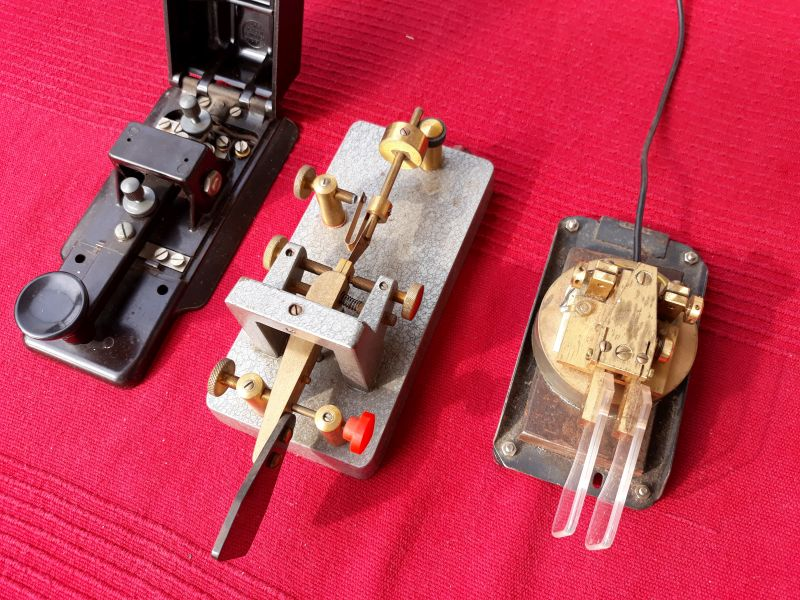
\includegraphics[width=0.85\textwidth]{foto/109}
    \caption{\scriptsize Morsetasten}
    \label{n_cwtast}
\end{figure}

   \end{column}
\end{columns}

\end{frame}

\begin{frame}
\begin{figure}
    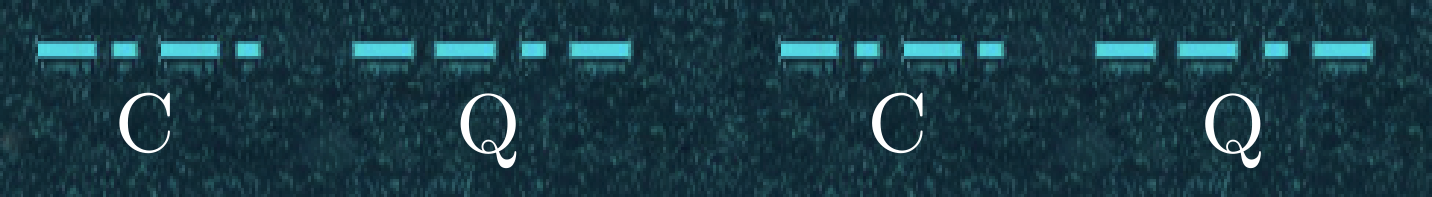
\includegraphics[width=0.85\textwidth]{foto/216}
    \caption{\scriptsize \enquote{CQ CQ} in Morsetelegrafie}
    \label{n_cqcq_horiz}
\end{figure}
\begin{itemize}
  \item Einigung darauf, was bestimmte Abfolgen unterschiedlicher Zeitabstände bedeuten
  \item Mitte des 19. Jahrhunderts Verständigung über den bis heute üblichen Morsecode
  \end{itemize}

\end{frame}

\begin{frame}
\frametitle{Telegrafie}
\begin{itemize}
  \item Übertragungsverfahren mit Hilfsmittel
  \item Rauch oder elektrische Schwingung wird so beeinflusst, um eine Nachricht zu übertragen
  \item Das Hilfsmittel ist der \emph{Träger}
  \item Im Funk aufgrund hoher Frequenzen auch \emph{Hochfrequenz-Träger} oder \emph{HF-Träger}
  \item Verfahren zum Ändern des Trägers ist die \emph{Modulation}
  \end{itemize}

\end{frame}

\begin{frame}
\only<1>{
\begin{QQuestion}{NE201}{Wie werden bei \glqq CW\grqq{} (Continuous Wave) Informationen übertragen?}{Durch Ein- und Ausschalten eines HF-Trägers}
{Durch Änderung der Trägerfrequenz in diskreten Stufen}
{Durch Modulation eines Subträgers}
{Durch diskrete Phasenmodulation}
\end{QQuestion}

}
\only<2>{
\begin{QQuestion}{NE201}{Wie werden bei \glqq CW\grqq{} (Continuous Wave) Informationen übertragen?}{\textbf{\textcolor{DARCgreen}{Durch Ein- und Ausschalten eines HF-Trägers}}}
{Durch Änderung der Trägerfrequenz in diskreten Stufen}
{Durch Modulation eines Subträgers}
{Durch diskrete Phasenmodulation}
\end{QQuestion}

}
\end{frame}

\begin{frame}
\only<1>{
\begin{QQuestion}{NE101}{Durch Modulation~...}{werden dem Signal NF-Komponenten entnommen.}
{wird einem oder mehreren Trägern Informationen entnommen.}
{werden Sprach- und CW-Signale kombiniert.}
{werden Informationen auf einen oder mehrere Träger übertragen.}
\end{QQuestion}

}
\only<2>{
\begin{QQuestion}{NE101}{Durch Modulation~...}{werden dem Signal NF-Komponenten entnommen.}
{wird einem oder mehreren Trägern Informationen entnommen.}
{werden Sprach- und CW-Signale kombiniert.}
{\textbf{\textcolor{DARCgreen}{werden Informationen auf einen oder mehrere Träger übertragen.}}}
\end{QQuestion}

}
\end{frame}

\begin{frame}
\frametitle{Andere Modulationsarten}
Die elektrische Schwingung kann auf andere Arten moduliert werden

\begin{itemize}
  \item Stärke (Amplitude)
  \item Periode (Frequenz)
  \end{itemize}
\end{frame}%ENDCONTENT


\section{Unmodulierter Träger}
\label{section:unmodulierter_traeger}
\begin{frame}%STARTCONTENT

\begin{columns}
    \begin{column}{0.48\textwidth}
    \begin{itemize}
  \item Einfachste Form eines HF-Signals
  \item Konstante Amplitude, Frequenz und Phasenlage
  \item Genau eine Frequenz
  \item Bereits Ein- und Ausschalten (CW) des Trägers ist eine Informationsübertragung
  \end{itemize}

    \end{column}
   \begin{column}{0.48\textwidth}
       
\begin{figure}
    \DARCimage{0.85\linewidth}{356include}
    \caption{\scriptsize Unmodulierter Träger}
    \label{e_unmodulierter_traeger}
\end{figure}


   \end{column}
\end{columns}

\end{frame}%ENDCONTENT


\section{Modulationsarten}
\label{section:modulationsarten}
\begin{frame}%STARTCONTENT

\begin{columns}
    \begin{column}{0.48\textwidth}
    
\begin{figure}
    \DARCimage{0.85\linewidth}{790include}
    \caption{\scriptsize Schwingung}
    \label{n_schwingung}
\end{figure}


    \end{column}
   \begin{column}{0.48\textwidth}
       Eigenschaften einer elektrischen Schwingung:

\begin{itemize}
  \item Amplitude
  \item Frequenz
  \end{itemize}

   \end{column}
\end{columns}

\end{frame}

\begin{frame}
\frametitle{Amplitudenmodulation (AM)}

\begin{figure}
    \DARCimage{0.85\linewidth}{358include}
    \caption{\scriptsize Bei der Amplitudenmodulation (AM) wird die Amplitude einer elektrischen Schwingung verändert.}
    \label{n_modulationsarten_am}
\end{figure}

\end{frame}

\begin{frame}
\frametitle{Frequenzmodulation (FM)}

\begin{figure}
    \DARCimage{0.85\linewidth}{357include}
    \caption{\scriptsize Bei der Frequenzmodulation (FM) wird die Schwingungsdauer und somit die Frequenz verändert.}
    \label{n_modulationsarten_am}
\end{figure}

\end{frame}%ENDCONTENT


\section{Sprachsignale}
\label{section:sprachsignale}
\begin{frame}%STARTCONTENT

\begin{figure}
    \DARCimage{0.85\linewidth}{742include}
    \caption{\scriptsize Menschliche Sprache im Amplitudenspektrum, links die tiefen und rechts die hohen Töne}
    \label{n_sprachspektrum}
\end{figure}

\end{frame}

\begin{frame}
\begin{columns}
    \begin{column}{0.48\textwidth}
    \begin{itemize}
  \item Sprechen wir in ein Mikrofon, dann wandelt es das Sprachsignal in elektrische Schwingungen um.
  \item Das Sprachsignal liegt nicht mehr als Schallwelle, sondern als elektrische Schwingung vor und kann im Funkgerät verarbeitet werden.
  \end{itemize}

    \end{column}
    \pause
    
   \begin{column}{0.48\textwidth}
       \begin{itemize}
  \item Die „Breite“ des Signals wird übrigens als \emph{Bandbreite} bezeichnet und in Hertz (Hz) angegeben.
  \item Angenommen es soll Sprache im Frequenzbereich von \qtyrange{300}{2700}{\hertz} übertragen werden.
  \item Die Bandbreite beträgt in diesem Falle \qty{2700}{\hertz} – \qty{300}{\hertz} = \qty{2400}{\hertz}
  \end{itemize}

   \end{column}
\end{columns}



\end{frame}

\begin{frame}
\only<1>{
\begin{QQuestion}{EA105}{Welche Einheit wird üblicherweise für die Bandbreite verwendet?}{Dezibel (dB)}
{Baud (Bd)}
{Bit pro Sekunde (Bit/s)}
{Hertz (Hz)}
\end{QQuestion}

}
\only<2>{
\begin{QQuestion}{EA105}{Welche Einheit wird üblicherweise für die Bandbreite verwendet?}{Dezibel (dB)}
{Baud (Bd)}
{Bit pro Sekunde (Bit/s)}
{\textbf{\textcolor{DARCgreen}{Hertz (Hz)}}}
\end{QQuestion}

}
\end{frame}%ENDCONTENT


\section{Amplitudenmodulation (AM)}
\label{section:am}
\begin{frame}%STARTCONTENT

\begin{columns}
    \begin{column}{0.48\textwidth}
    
\begin{figure}
    \DARCimage{0.85\linewidth}{716include}
    \caption{\scriptsize Signal eines AM-Rundfunksenders (Sprache / Musik)}
    \label{n_Wasserfall0}
\end{figure}


    \end{column}
   \begin{column}{0.48\textwidth}
       \begin{itemize}
  \item Modulationssignal wird durch Änderung der Amplitude auf den Träger aufmoduliert
  \item Frequenz des Trägers bleibt unverändert
  \item Änderung der Amplitude ändert die Form des Trägers $\rightarrow$ entspricht nicht mehr einer Sinusschwingung
  \item Zusätzliche Frequenzen heißen \emph{Seitenbänder}
  \end{itemize}

   \end{column}
\end{columns}

\end{frame}

\begin{frame}
\begin{columns}
    \begin{column}{0.48\textwidth}
    \begin{itemize}
  \item In den Seitenbändern steckt die übertragene Information, also z.\,B. die Sprache
  \item Die von AM belegte \emph{Bandbreite} ist doppelt so hoch wie die höchste Frequenz des Modulationssignals
  \end{itemize}

    \end{column}
   \begin{column}{0.48\textwidth}
       
\begin{figure}
    \DARCimage{0.85\linewidth}{476include}
    \caption{\scriptsize Symbolische Darstellung eines amplitudenmodulierten Signals mit Träger und Seitenbändern}
    \label{n_seitenband}
\end{figure}


   \end{column}
\end{columns}

\end{frame}

\begin{frame}
\only<1>{
\begin{QQuestion}{NE202}{Welche Aussage zur Amplitudenmodulation ist richtig? Durch das Informationssignal~...}{wird die Amplitude des Trägers beeinflusst. Die Frequenz des Trägers bleibt dabei konstant.}
{wird die Frequenz des Trägers beeinflusst. Die Amplitude des Trägers bleibt dabei konstant.}
{werden gleichzeitig Amplitude und Frequenz des Trägers beeinflusst.}
{werden nacheinander Amplitude und Frequenz des Trägers beeinflusst.}
\end{QQuestion}

}
\only<2>{
\begin{QQuestion}{NE202}{Welche Aussage zur Amplitudenmodulation ist richtig? Durch das Informationssignal~...}{\textbf{\textcolor{DARCgreen}{wird die Amplitude des Trägers beeinflusst. Die Frequenz des Trägers bleibt dabei konstant.}}}
{wird die Frequenz des Trägers beeinflusst. Die Amplitude des Trägers bleibt dabei konstant.}
{werden gleichzeitig Amplitude und Frequenz des Trägers beeinflusst.}
{werden nacheinander Amplitude und Frequenz des Trägers beeinflusst.}
\end{QQuestion}

}
\end{frame}

\begin{frame}
\only<1>{
\begin{PQuestion}{NE206}{Welche spektrale Darstellung ergibt sich für die Modulationsart AM bei diesem  Audiospektrum?}{\DARCimage{1.0\linewidth}{477include}}
{\DARCimage{1.0\linewidth}{476include}}
{\DARCimage{1.0\linewidth}{478include}}
{\DARCimage{1.0\linewidth}{479include}}
{\DARCimage{1.0\linewidth}{475include}}\end{PQuestion}

}
\only<2>{
\begin{PQuestion}{NE206}{Welche spektrale Darstellung ergibt sich für die Modulationsart AM bei diesem  Audiospektrum?}{\DARCimage{1.0\linewidth}{477include}}
{\textbf{\textcolor{DARCgreen}{\DARCimage{1.0\linewidth}{476include}}}}
{\DARCimage{1.0\linewidth}{478include}}
{\DARCimage{1.0\linewidth}{479include}}
{\DARCimage{1.0\linewidth}{475include}}\end{PQuestion}

}
\end{frame}%ENDCONTENT


\section{Amplitudenmodulation (AM) II}
\label{section:am_2}
\begin{frame}%STARTCONTENT

\only<1>{
\begin{question2x2}{AE201}{In welcher Abbildung ist AM mit einem Modulationsgrad von \qty{100}{\percent} dargestellt?}{\DARCimage{1.0\linewidth}{24include}}
{\DARCimage{1.0\linewidth}{27include}}
{\DARCimage{1.0\linewidth}{28include}}
{\DARCimage{1.0\linewidth}{26include}}
\end{question2x2}

}
\only<2>{
\begin{question2x2}{AE201}{In welcher Abbildung ist AM mit einem Modulationsgrad von \qty{100}{\percent} dargestellt?}{\textbf{\textcolor{DARCgreen}{\DARCimage{1.0\linewidth}{24include}}}}
{\DARCimage{1.0\linewidth}{27include}}
{\DARCimage{1.0\linewidth}{28include}}
{\DARCimage{1.0\linewidth}{26include}}
\end{question2x2}

}
\end{frame}

\begin{frame}
\only<1>{
\begin{PQuestion}{AE202}{Das folgende Oszillogramm zeigt ein AM-Signal. Der Modulationsgrad beträgt hier ca.}{\qty{50}{\percent}.}
{\qty{33}{\percent}.}
{\qty{67}{\percent}.}
{\qty{75}{\percent}.}
{\DARCimage{1.0\linewidth}{78include}}\end{PQuestion}

}
\only<2>{
\begin{PQuestion}{AE202}{Das folgende Oszillogramm zeigt ein AM-Signal. Der Modulationsgrad beträgt hier ca.}{\textbf{\textcolor{DARCgreen}{\qty{50}{\percent}.}}}
{\qty{33}{\percent}.}
{\qty{67}{\percent}.}
{\qty{75}{\percent}.}
{\DARCimage{1.0\linewidth}{78include}}\end{PQuestion}

}
\end{frame}

\begin{frame}
\only<1>{
\begin{question2x2}{AE203}{Welches Bild stellt die Übermodulation eines AM-Signals dar?}{\DARCimage{1.0\linewidth}{24include}}
{\DARCimage{1.0\linewidth}{28include}}
{\DARCimage{1.0\linewidth}{25include}}
{\DARCimage{1.0\linewidth}{26include}}
\end{question2x2}

}
\only<2>{
\begin{question2x2}{AE203}{Welches Bild stellt die Übermodulation eines AM-Signals dar?}{\DARCimage{1.0\linewidth}{24include}}
{\textbf{\textcolor{DARCgreen}{\DARCimage{1.0\linewidth}{28include}}}}
{\DARCimage{1.0\linewidth}{25include}}
{\DARCimage{1.0\linewidth}{26include}}
\end{question2x2}

}
\end{frame}

\begin{frame}
\only<1>{
\begin{QQuestion}{AE204}{Um Seitenband-Splatter zu vermeiden, sollte der Modulationsgrad eines AM-Signals unter~...}{\qty{100}{\percent}~liegen.}
{\qty{50}{\percent}~liegen.}
{\qty{75}{\percent}~liegen.}
{\qty{25}{\percent}~liegen.}
\end{QQuestion}

}
\only<2>{
\begin{QQuestion}{AE204}{Um Seitenband-Splatter zu vermeiden, sollte der Modulationsgrad eines AM-Signals unter~...}{\textbf{\textcolor{DARCgreen}{\qty{100}{\percent}~liegen.}}}
{\qty{50}{\percent}~liegen.}
{\qty{75}{\percent}~liegen.}
{\qty{25}{\percent}~liegen.}
\end{QQuestion}

}
\end{frame}%ENDCONTENT


\section{Einseitenbandmodulation (SSB)}
\label{section:ssb}
\begin{frame}%STARTCONTENT

\begin{columns}
    \begin{column}{0.48\textwidth}
    
\begin{figure}
    \DARCimage{0.85\linewidth}{482include}
    \caption{\scriptsize Amplitudenmodulation, Träger mit unterem (a) und oberen (b) Seitenband}
    \label{n_seitenband}
\end{figure}


    \end{column}
   \begin{column}{0.48\textwidth}
       \begin{itemize}
  \item Bei Amplitudenmodulation zusätzlich zum Träger zwei Seitenbänder $\rightarrow$ unteres bzw. oberes Seitenband
  \item \enquote{lower side band} (\emph{LSB}) und \enquote{upper side band} (\emph{USB})
  \item Der Träger selbst enthält gar keine Information
  \end{itemize}

   \end{column}
\end{columns}

\end{frame}

\begin{frame}
\begin{columns}
    \begin{column}{0.48\textwidth}
    \begin{itemize}
  \item Es reicht also, nur ein Seitenband auszusenden und auf den Träger und das andere Seitenband zu verzichten
  \item Gesamte Sendeleistung wird für die Übertragung der Information genutzt
  \item Belegte Bandbreite entspricht der Bandbreite des aufmodulierten Signals
  \end{itemize}

    \end{column}
   \begin{column}{0.48\textwidth}
       
\begin{figure}
    \DARCimage{0.85\linewidth}{743include}
    \caption{\scriptsize Seitenbänder bei AM, LSB und USB im Vergleich}
    \label{n_seitenband}
\end{figure}

\emph{Einseitenbandmodulation} bzw. \emph{single-sideband (SSB)}


   \end{column}
\end{columns}

\end{frame}

\begin{frame}USB steht für \emph{Upper Side Band}

(im Deutschen wird es gerne mit Unteres Seitenband verwechselt)

\end{frame}

\begin{frame}
\only<1>{
\begin{QQuestion}{NE203}{Was ist der Unterschied zwischen AM und SSB?}{AM hat keinen Träger und zwei Seitenbänder, SSB arbeitet mit Träger und nur einem Seitenband.}
{AM hat einen Träger und ein Seitenband, SSB arbeitet mit Trägerunterdrückung und hat zwei Seitenbänder.}
{AM hat keinen Träger und zwei Seitenbänder, SSB arbeitet mit Trägerunterdrückung und nur einem Seitenband.}
{AM hat einen Träger und zwei Seitenbänder, SSB arbeitet mit Trägerunterdrückung und nur einem Seitenband.}
\end{QQuestion}

}
\only<2>{
\begin{QQuestion}{NE203}{Was ist der Unterschied zwischen AM und SSB?}{AM hat keinen Träger und zwei Seitenbänder, SSB arbeitet mit Träger und nur einem Seitenband.}
{AM hat einen Träger und ein Seitenband, SSB arbeitet mit Trägerunterdrückung und hat zwei Seitenbänder.}
{AM hat keinen Träger und zwei Seitenbänder, SSB arbeitet mit Trägerunterdrückung und nur einem Seitenband.}
{\textbf{\textcolor{DARCgreen}{AM hat einen Träger und zwei Seitenbänder, SSB arbeitet mit Trägerunterdrückung und nur einem Seitenband.}}}
\end{QQuestion}

}
\end{frame}

\begin{frame}
\only<1>{
\begin{QQuestion}{NE204}{Was ist der Unterschied zwischen LSB und USB?}{LSB arbeitet mit Trägerunterdrückung und dem unteren Seitenband, USB arbeitet mit Trägerunterdrückung und dem oberen Seitenband.}
{LSB arbeitet mit Träger und zwei Seitenbändern, USB arbeitet mit Trägerunterdrückung und einem Seitenband.}
{LSB arbeitet mit Träger und einem Seitenband, USB arbeitet mit Trägerunterdrückung und beiden Seitenbändern.}
{LSB arbeitet mit Trägerunterdrückung und dem linken Seitenband, USB arbeitet mit Trägerunterdrückung und dem unteren Seitenband.}
\end{QQuestion}

}
\only<2>{
\begin{QQuestion}{NE204}{Was ist der Unterschied zwischen LSB und USB?}{\textbf{\textcolor{DARCgreen}{LSB arbeitet mit Trägerunterdrückung und dem unteren Seitenband, USB arbeitet mit Trägerunterdrückung und dem oberen Seitenband.}}}
{LSB arbeitet mit Träger und zwei Seitenbändern, USB arbeitet mit Trägerunterdrückung und einem Seitenband.}
{LSB arbeitet mit Träger und einem Seitenband, USB arbeitet mit Trägerunterdrückung und beiden Seitenbändern.}
{LSB arbeitet mit Trägerunterdrückung und dem linken Seitenband, USB arbeitet mit Trägerunterdrückung und dem unteren Seitenband.}
\end{QQuestion}

}
\end{frame}

\begin{frame}
\only<1>{
\begin{PQuestion}{NE208}{Welche spektrale Darstellung ergibt sich für Einseitenbandmodulation in LSB bei diesem Audiospektrum?}{\DARCimage{1.0\linewidth}{477include}}
{\DARCimage{1.0\linewidth}{480include}}
{\DARCimage{1.0\linewidth}{479include}}
{\DARCimage{1.0\linewidth}{481include}}
{\DARCimage{1.0\linewidth}{475include}}\end{PQuestion}

}
\only<2>{
\begin{PQuestion}{NE208}{Welche spektrale Darstellung ergibt sich für Einseitenbandmodulation in LSB bei diesem Audiospektrum?}{\DARCimage{1.0\linewidth}{477include}}
{\DARCimage{1.0\linewidth}{480include}}
{\DARCimage{1.0\linewidth}{479include}}
{\textbf{\textcolor{DARCgreen}{\DARCimage{1.0\linewidth}{481include}}}}
{\DARCimage{1.0\linewidth}{475include}}\end{PQuestion}

}
\end{frame}

\begin{frame}
\only<1>{
\begin{PQuestion}{NE207}{Welche spektrale Darstellung ergibt sich für Einseitenbandmodulation in USB bei diesem Audiospektrum?}{\DARCimage{1.0\linewidth}{481include}}
{\DARCimage{1.0\linewidth}{480include}}
{\DARCimage{1.0\linewidth}{479include}}
{\DARCimage{1.0\linewidth}{477include}}
{\DARCimage{1.0\linewidth}{475include}}\end{PQuestion}

}
\only<2>{
\begin{PQuestion}{NE207}{Welche spektrale Darstellung ergibt sich für Einseitenbandmodulation in USB bei diesem Audiospektrum?}{\DARCimage{1.0\linewidth}{481include}}
{\textbf{\textcolor{DARCgreen}{\DARCimage{1.0\linewidth}{480include}}}}
{\DARCimage{1.0\linewidth}{479include}}
{\DARCimage{1.0\linewidth}{477include}}
{\DARCimage{1.0\linewidth}{475include}}\end{PQuestion}

}
\end{frame}

\begin{frame}
\only<1>{
\begin{PQuestion}{NE205}{Welche Begriffe sind den Bereichen a und b des Modulationsverfahrens AM zuzuordnen?}{a = LSB; b = USB}
{a = USB; b = LSB}
{a = DSB; b = SSB}
{a = NF; b = HF}
{\DARCimage{1.0\linewidth}{482include}}\end{PQuestion}

}
\only<2>{
\begin{PQuestion}{NE205}{Welche Begriffe sind den Bereichen a und b des Modulationsverfahrens AM zuzuordnen?}{\textbf{\textcolor{DARCgreen}{a = LSB; b = USB}}}
{a = USB; b = LSB}
{a = DSB; b = SSB}
{a = NF; b = HF}
{\DARCimage{1.0\linewidth}{482include}}\end{PQuestion}

}
\end{frame}%ENDCONTENT


\section{Einseitenbandmodulation (SSB) II}
\label{section:ssb_2}
\begin{frame}%STARTCONTENT

\frametitle{Bandbreite}
\begin{columns}
    \begin{column}{0.48\textwidth}
    \begin{itemize}
  \item Im Gegensatz zu AM wird weniger als die halbe Bandbreite verwendet
  \item Maximal \qty{2,7}{\kilo\hertz}
  \item Entspricht dem NF-Signal
  \end{itemize}

    \end{column}
   \begin{column}{0.48\textwidth}
       
\begin{figure}
    \DARCimage{0.85\linewidth}{743include}
    \caption{\scriptsize Bandbreite von AM, USB und LSB}
    \label{e_bandbreite_am_ssb}
\end{figure}


   \end{column}
\end{columns}

\end{frame}

\begin{frame}
\only<1>{
\begin{QQuestion}{EE201}{Wie unterscheidet sich SSB von AM in Bezug auf die Bandbreite?}{SSB beansprucht etwa 1/4 Bandbreite der Modulationsart AM.}
{SSB beansprucht etwas mehr als die halbe Bandbreite der Modulationsart AM.}
{SSB beansprucht weniger als die halbe Bandbreite der Modulationsart AM.}
{SSB und AM lassen keinen Vergleich zu, da sie grundverschieden erzeugt werden.}
\end{QQuestion}

}
\only<2>{
\begin{QQuestion}{EE201}{Wie unterscheidet sich SSB von AM in Bezug auf die Bandbreite?}{SSB beansprucht etwa 1/4 Bandbreite der Modulationsart AM.}
{SSB beansprucht etwas mehr als die halbe Bandbreite der Modulationsart AM.}
{\textbf{\textcolor{DARCgreen}{SSB beansprucht weniger als die halbe Bandbreite der Modulationsart AM.}}}
{SSB und AM lassen keinen Vergleich zu, da sie grundverschieden erzeugt werden.}
\end{QQuestion}

}
\end{frame}

\begin{frame}
\only<1>{
\begin{QQuestion}{EE202}{Wie groß ist in etwa die HF-Bandbreite, die für die Übertragung eines SSB-Signals erforderlich ist?}{Sie entspricht der Hälfte der Bandbreite des NF-Signals.}
{Sie entspricht der Bandbreite des NF-Signals.}
{Sie entspricht der doppelten Bandbreite des NF-Signals.}
{Sie ist Null, weil bei SSB-Modulation der HF-Träger unterdrückt wird.}
\end{QQuestion}

}
\only<2>{
\begin{QQuestion}{EE202}{Wie groß ist in etwa die HF-Bandbreite, die für die Übertragung eines SSB-Signals erforderlich ist?}{Sie entspricht der Hälfte der Bandbreite des NF-Signals.}
{\textbf{\textcolor{DARCgreen}{Sie entspricht der Bandbreite des NF-Signals.}}}
{Sie entspricht der doppelten Bandbreite des NF-Signals.}
{Sie ist Null, weil bei SSB-Modulation der HF-Träger unterdrückt wird.}
\end{QQuestion}

}
\end{frame}

\begin{frame}
\only<1>{
\begin{QQuestion}{EJ210}{Um Störungen auf benachbarten Frequenzen zu minimieren, sollte die Übertragungsbandbreite bei SSB~...}{höchstens \qty{1,8}{\kHz} betragen.}
{höchstens \qty{2,7}{\kHz} betragen.}
{höchstens \qty{3,1}{\kHz} betragen.}
{höchstens \qty{15,0}{\kHz} betragen.}
\end{QQuestion}

}
\only<2>{
\begin{QQuestion}{EJ210}{Um Störungen auf benachbarten Frequenzen zu minimieren, sollte die Übertragungsbandbreite bei SSB~...}{höchstens \qty{1,8}{\kHz} betragen.}
{\textbf{\textcolor{DARCgreen}{höchstens \qty{2,7}{\kHz} betragen.}}}
{höchstens \qty{3,1}{\kHz} betragen.}
{höchstens \qty{15,0}{\kHz} betragen.}
\end{QQuestion}

}
\end{frame}

\begin{frame}
\frametitle{Modulation}
\begin{columns}
    \begin{column}{0.48\textwidth}
    \begin{itemize}
  \item Durch Mischung und Filterung
  \item Mit der Vorauswahl von USB und LSB wird die Trägerfrequenz gewählt
  \item Durch den Mischer entstehen zwei Frequenzen
  \item Im Bandfilter wird nur eine Frequenz durchgelassen
  \end{itemize}

    \end{column}
   \begin{column}{0.48\textwidth}
       
\begin{figure}
    \DARCimage{0.85\linewidth}{500include}
    \caption{\scriptsize Blockschaltbild zur Modulation von SSB mit der Filtermethode}
    \label{e_ssb_modulation}
\end{figure}


   \end{column}
\end{columns}

\end{frame}

\begin{frame}
\begin{columns}
    \begin{column}{0.48\textwidth}
    \begin{itemize}
  \item Der Trick ist hier, dass das Bandfilter nur eine Resonanzfrequenz hat
  \item Durch die Verschiebung der Trägerfrequenz im Oszillator wird dann das gewünschte Seitenband durchgelassen
  \end{itemize}

    \end{column}
   \begin{column}{0.48\textwidth}
       
\begin{figure}
    \DARCimage{0.85\linewidth}{500include}
    \caption{\scriptsize Blockschaltbild zur Modulation von SSB mit der Filtermethode}
    \label{e_ssb_modulation}
\end{figure}


   \end{column}
\end{columns}

\end{frame}

\begin{frame}
\begin{columns}
    \begin{column}{0.48\textwidth}
    Beispiel LSB:

\begin{itemize}
  \item Mikrofon: \qty{300}{\hertz} -- \qty{3}{\kilo\hertz}
  \item LSB-Oszillator: \qty{9001,5}{\kilo\hertz}
  \item DSB-Signal:<br/> a) 8998,5 -- 9001,2<br/> b) 9001,8 -- 9004,5 
  \item Filter: \qty{9000}{\kilo\hertz}  $\pm$  \qty{1,5}{\kilo\hertz}
  \item SSB-Signal:<br/> \qtyrange{8998,5}{9001,2}{\kilo\hertz}
  \end{itemize}

    \end{column}
   \begin{column}{0.48\textwidth}
       
\begin{figure}
    \DARCimage{0.85\linewidth}{831include}
    \caption{\scriptsize Frequenzen mit der Filtermethode bei LSB}
    \label{e_ssb_modulation_lsb}
\end{figure}


   \end{column}
\end{columns}

\end{frame}

\begin{frame}
\begin{columns}
    \begin{column}{0.48\textwidth}
    Beispiel USB:

\begin{itemize}
  \item Mikrofon: \qty{300}{\hertz} -- \qty{3}{\kilo\hertz}
  \item USB-Oszillator: \qty{8998,5}{\kilo\hertz}
  \item DSB-Signal:<br/> a) \qtyrange{8995,5}{8998,2}{\kilo\hertz}<br/> b) \qtyrange{8998,8}{9001,5}{\kilo\hertz}
  \item Filter: \qty{9000}{\kilo\hertz}  $\pm$  \qty{1,5}{\kilo\hertz}
  \item SSB-Signal:<br/> \qtyrange{8998,8}{9001,5}{\kilo\hertz}
  \end{itemize}

    \end{column}
   \begin{column}{0.48\textwidth}
       
\begin{figure}
    \DARCimage{0.85\linewidth}{832include}
    \caption{\scriptsize Frequenzen mit der Filtermethode bei USB}
    \label{e_ssb_modulation_usb}
\end{figure}


   \end{column}
\end{columns}

\end{frame}

\begin{frame}
\only<1>{
\begin{QQuestion}{EE203}{Ein Träger von \qty{21,250}{\MHz} wird mit der NF-Frequenz von \qty{1}{\kHz} in SSB (USB) moduliert. Welche Frequenz tritt im ideal modulierten HF-Signal auf?}{\qty{21,260}{\MHz}}
{\qty{21,250}{\MHz}}
{\qty{21,249}{\MHz}}
{\qty{21,251}{\MHz}}
\end{QQuestion}

}
\only<2>{
\begin{QQuestion}{EE203}{Ein Träger von \qty{21,250}{\MHz} wird mit der NF-Frequenz von \qty{1}{\kHz} in SSB (USB) moduliert. Welche Frequenz tritt im ideal modulierten HF-Signal auf?}{\qty{21,260}{\MHz}}
{\qty{21,250}{\MHz}}
{\qty{21,249}{\MHz}}
{\textbf{\textcolor{DARCgreen}{\qty{21,251}{\MHz}}}}
\end{QQuestion}

}
\end{frame}

\begin{frame}
\only<1>{
\begin{QQuestion}{EE204}{Ein Träger von \qty{3,65}{\MHz} wird mit der NF-Frequenz von \qty{2}{\kHz} in SSB (LSB) moduliert. Welche Frequenz/Frequenzen treten im modulierten HF-Signal hauptsächlich auf?}{\qty{3,648}{\MHz} und \qty{3,650}{\MHz}}
{\qty{3,648}{\MHz}}
{\qty{3,652}{\MHz}}
{\qty{3,648}{\MHz} und \qty{3,652}{\MHz}}
\end{QQuestion}

}
\only<2>{
\begin{QQuestion}{EE204}{Ein Träger von \qty{3,65}{\MHz} wird mit der NF-Frequenz von \qty{2}{\kHz} in SSB (LSB) moduliert. Welche Frequenz/Frequenzen treten im modulierten HF-Signal hauptsächlich auf?}{\qty{3,648}{\MHz} und \qty{3,650}{\MHz}}
{\textbf{\textcolor{DARCgreen}{\qty{3,648}{\MHz}}}}
{\qty{3,652}{\MHz}}
{\qty{3,648}{\MHz} und \qty{3,652}{\MHz}}
\end{QQuestion}

}
\end{frame}

\begin{frame}
\frametitle{NF-Signal}
\begin{columns}
    \begin{column}{0.48\textwidth}
    \begin{itemize}
  \item Für Sprache reicht zwischen 300 und \qty{3000}{\hertz}
  \item Entspricht \qty{2,7}{\kilo\hertz}
  \item Es werden auch kleinere Filter, z.B. \qty{2,4}{\kilo\hertz} verwendet
  \item An vielen TRX lassen sich die Filter einstellen
  \end{itemize}

    \end{column}
   \begin{column}{0.48\textwidth}
       \begin{itemize}
  \item Wird ein NF-Signal mit größerer Bandbreite verwendet, steigt die HF-Bandbreite
  \item Sollte vermieden werden, um benachbarte Signale nicht zu stören
  \item Auf maximale Bandbreite im Bandplan achten
  \end{itemize}

   \end{column}
\end{columns}

\end{frame}

\begin{frame}
\only<1>{
\begin{QQuestion}{EJ211}{Um etwaige Funkstörungen auf Nachbarfrequenzen zu begrenzen, sollte bei SSB-Telefonie die höchste zu übertragende NF-Frequenz~...}{unter \qty{3}{\kHz} liegen.}
{unter \qty{1}{\kHz} liegen.}
{unter \qty{5}{\kHz} liegen.}
{unter \qty{10}{\kHz} liegen.}
\end{QQuestion}

}
\only<2>{
\begin{QQuestion}{EJ211}{Um etwaige Funkstörungen auf Nachbarfrequenzen zu begrenzen, sollte bei SSB-Telefonie die höchste zu übertragende NF-Frequenz~...}{\textbf{\textcolor{DARCgreen}{unter \qty{3}{\kHz} liegen.}}}
{unter \qty{1}{\kHz} liegen.}
{unter \qty{5}{\kHz} liegen.}
{unter \qty{10}{\kHz} liegen.}
\end{QQuestion}

}

\end{frame}

\begin{frame}
\only<1>{
\begin{QQuestion}{EF310}{Welche Bandbreite sollte das nachgeschaltete Filter zur Unterdrückung eines Seitenbandes bei der Erzeugung eines SSB-Telefoniesignals haben?}{\qty{455}{\kHz} }
{\qty{800}{\Hz} }
{\qty{2,4}{\kHz} }
{\qty{10,7}{\MHz} }
\end{QQuestion}

}
\only<2>{
\begin{QQuestion}{EF310}{Welche Bandbreite sollte das nachgeschaltete Filter zur Unterdrückung eines Seitenbandes bei der Erzeugung eines SSB-Telefoniesignals haben?}{\qty{455}{\kHz} }
{\qty{800}{\Hz} }
{\textbf{\textcolor{DARCgreen}{\qty{2,4}{\kHz} }}}
{\qty{10,7}{\MHz} }
\end{QQuestion}

}
\end{frame}

\begin{frame}
\only<1>{
\begin{QQuestion}{EE207}{Wie groß ist die Bandbreite von CW im Vergleich zu einem Sprachsignal in SSB oder AM?}{In beiden Fällen weist CW eine kleinere Bandbreite auf.}
{In beiden Fällen weist CW eine größere Bandbreite auf.}
{Die Bandbreite von CW ist kleiner als bei SSB, jedoch größer als bei AM.}
{Die Bandbreite von CW ist größer als bei SSB, jedoch kleiner als bei AM.}
\end{QQuestion}

}
\only<2>{
\begin{QQuestion}{EE207}{Wie groß ist die Bandbreite von CW im Vergleich zu einem Sprachsignal in SSB oder AM?}{\textbf{\textcolor{DARCgreen}{In beiden Fällen weist CW eine kleinere Bandbreite auf.}}}
{In beiden Fällen weist CW eine größere Bandbreite auf.}
{Die Bandbreite von CW ist kleiner als bei SSB, jedoch größer als bei AM.}
{Die Bandbreite von CW ist größer als bei SSB, jedoch kleiner als bei AM.}
\end{QQuestion}

}
\end{frame}

\begin{frame}
\frametitle{Mikrofonverstärkung}
\begin{itemize}
  \item Mit der NF-Leistung wird die Leistung der HF gesteuert
  \item Zu leises Mikrofon bewirkt weniger Ausgangleistung am Sender
  \item Eine zu starke Mikrofonverstärkung kann Störungen bei Stationen auf dicht benachbarten Frequenzen verursachen
  \end{itemize}
\end{frame}

\begin{frame}
\only<1>{
\begin{QQuestion}{EE206}{Was bewirkt eine zu geringe Mikrofonverstärkung bei einem SSB-Transceiver?}{Störungen bei Stationen, die auf dicht benachbarten Frequenzen arbeiten}
{Störungen von Stationen, die auf einem anderen Frequenzband arbeiten}
{geringe Bandbreite}
{geringe Ausgangsleistung}
\end{QQuestion}

}
\only<2>{
\begin{QQuestion}{EE206}{Was bewirkt eine zu geringe Mikrofonverstärkung bei einem SSB-Transceiver?}{Störungen bei Stationen, die auf dicht benachbarten Frequenzen arbeiten}
{Störungen von Stationen, die auf einem anderen Frequenzband arbeiten}
{geringe Bandbreite}
{\textbf{\textcolor{DARCgreen}{geringe Ausgangsleistung}}}
\end{QQuestion}

}
\end{frame}

\begin{frame}
\only<1>{
\begin{QQuestion}{EE205}{Welche der aufgeführten Maßnahmen verringert die Ausgangsleistung eines SSB-Senders?}{Lauter ins Mikrofon sprechen }
{Verringern der NF-Amplitude}
{Verringern der Squelcheinstellung }
{Erhöhen der NF-Bandbreite}
\end{QQuestion}

}
\only<2>{
\begin{QQuestion}{EE205}{Welche der aufgeführten Maßnahmen verringert die Ausgangsleistung eines SSB-Senders?}{Lauter ins Mikrofon sprechen }
{\textbf{\textcolor{DARCgreen}{Verringern der NF-Amplitude}}}
{Verringern der Squelcheinstellung }
{Erhöhen der NF-Bandbreite}
\end{QQuestion}

}
\end{frame}

\begin{frame}
\only<1>{
\begin{QQuestion}{EJ215}{Was bewirkt in der Regel eine zu hohe Mikrofonverstärkung bei einem SSB-Transceiver?}{Störungen bei Stationen, die auf dicht benachbarten Frequenzen arbeiten}
{Störungen von Stationen, die auf einem anderen Frequenzband arbeiten}
{Störungen der Stromversorgung des Transceivers}
{Störungen von anderen elektronischen Geräten}
\end{QQuestion}

}
\only<2>{
\begin{QQuestion}{EJ215}{Was bewirkt in der Regel eine zu hohe Mikrofonverstärkung bei einem SSB-Transceiver?}{\textbf{\textcolor{DARCgreen}{Störungen bei Stationen, die auf dicht benachbarten Frequenzen arbeiten}}}
{Störungen von Stationen, die auf einem anderen Frequenzband arbeiten}
{Störungen der Stromversorgung des Transceivers}
{Störungen von anderen elektronischen Geräten}
\end{QQuestion}

}
\end{frame}%ENDCONTENT


\section{Einseitenbandmodulation (SSB) III}
\label{section:ssb_3}
\begin{frame}%STARTCONTENT

\only<1>{
\begin{QQuestion}{AE205}{Ein übermoduliertes SSB-Sendesignal führt zu~...}{Splatter-Erscheinungen.}
{Kreuzmodulation.}
{verminderten Seitenbändern.}
{überhöhtem Hub.}
\end{QQuestion}

}
\only<2>{
\begin{QQuestion}{AE205}{Ein übermoduliertes SSB-Sendesignal führt zu~...}{\textbf{\textcolor{DARCgreen}{Splatter-Erscheinungen.}}}
{Kreuzmodulation.}
{verminderten Seitenbändern.}
{überhöhtem Hub.}
\end{QQuestion}

}
\end{frame}

\begin{frame}
\only<1>{
\begin{PQuestion}{AE207}{Das folgende Oszillogramm zeigt~...}{ein typisches \qty{100}{\percent}-AM-Signal.}
{ein typisches Einton-FM-Testsignal.}
{ein typisches Zweiton-SSB-Testsignal.}
{ein typisches CW-Signal.}
{\DARCimage{1.0\linewidth}{43include}}\end{PQuestion}

}
\only<2>{
\begin{PQuestion}{AE207}{Das folgende Oszillogramm zeigt~...}{ein typisches \qty{100}{\percent}-AM-Signal.}
{ein typisches Einton-FM-Testsignal.}
{\textbf{\textcolor{DARCgreen}{ein typisches Zweiton-SSB-Testsignal.}}}
{ein typisches CW-Signal.}
{\DARCimage{1.0\linewidth}{43include}}\end{PQuestion}

}
\end{frame}

\begin{frame}
\only<1>{
\begin{QQuestion}{AE208}{Um Bandbreite einzusparen, sollte der Frequenzumfang eines NF-Sprachsignals, das an einen SSB-Modulator angelegt wird,~...}{\qty{1,8}{\kHz} nicht überschreiten.}
{\qty{2,7}{\kHz} nicht überschreiten.}
{\qty{800}{\Hz} nicht überschreiten.}
{\qty{15}{\kHz} nicht überschreiten.}
\end{QQuestion}

}
\only<2>{
\begin{QQuestion}{AE208}{Um Bandbreite einzusparen, sollte der Frequenzumfang eines NF-Sprachsignals, das an einen SSB-Modulator angelegt wird,~...}{\qty{1,8}{\kHz} nicht überschreiten.}
{\textbf{\textcolor{DARCgreen}{\qty{2,7}{\kHz} nicht überschreiten.}}}
{\qty{800}{\Hz} nicht überschreiten.}
{\qty{15}{\kHz} nicht überschreiten.}
\end{QQuestion}

}
\end{frame}

\begin{frame}
\only<1>{
\begin{QQuestion}{AE209}{Wie groß sollte der Abstand der Sendefrequenz zwischen zwei SSB-Signalen sein, um gegenseitige Störungen in SSB-Telefonie auf ein Mindestmaß zu begrenzen?}{\qty{25}{\kHz}}
{\qty{12,5}{\kHz}}
{\qty{3}{\kHz}}
{\qty{455}{\kHz}}
\end{QQuestion}

}
\only<2>{
\begin{QQuestion}{AE209}{Wie groß sollte der Abstand der Sendefrequenz zwischen zwei SSB-Signalen sein, um gegenseitige Störungen in SSB-Telefonie auf ein Mindestmaß zu begrenzen?}{\qty{25}{\kHz}}
{\qty{12,5}{\kHz}}
{\textbf{\textcolor{DARCgreen}{\qty{3}{\kHz}}}}
{\qty{455}{\kHz}}
\end{QQuestion}

}
\end{frame}

\begin{frame}
\only<1>{
\begin{QQuestion}{AE213}{Welche Aufgabe hat der Equalizer in einem SSB-Sender?}{Er dient zur Anpassung des Mikrofonfrequenzgangs an den Operator.}
{Er dient zur Erzeugung des SSB-Signals.}
{Er dient zur Unterdrückung von Oberschwingungen im Sendesignal.}
{Er dient zur Erhöhung der Trägerunterdrückung.}
\end{QQuestion}

}
\only<2>{
\begin{QQuestion}{AE213}{Welche Aufgabe hat der Equalizer in einem SSB-Sender?}{\textbf{\textcolor{DARCgreen}{Er dient zur Anpassung des Mikrofonfrequenzgangs an den Operator.}}}
{Er dient zur Erzeugung des SSB-Signals.}
{Er dient zur Unterdrückung von Oberschwingungen im Sendesignal.}
{Er dient zur Erhöhung der Trägerunterdrückung.}
\end{QQuestion}

}
\end{frame}%ENDCONTENT


\section{Frequenzmodulation (FM)}
\label{section:fm}
\begin{frame}%STARTCONTENT

\begin{figure}
    \DARCimage{0.85\linewidth}{357include}
    \caption{\scriptsize Frequenzmodulation}
    \label{n_fm_frequenzmodulation}
\end{figure}

\begin{itemize}
  \item Modulationssignal wird durch Änderung der Frequenz auf den Träger aufmoduliert
  \item Amplitude des Trägers wird nicht verändert und bleibt idealerweise konstant
  \end{itemize}
\end{frame}

\begin{frame}
\only<1>{
\begin{QQuestion}{NE301}{Welche Aussage zur Frequenzmodulation ist richtig? Durch das Informationssignal~...}{wird die Frequenz des Trägers beeinflusst. Die Amplitude des Trägers bleibt dabei konstant.}
{wird die Amplitude des Trägers beeinflusst. Die Frequenz des Trägers bleibt dabei konstant. }
{werden gleichzeitig Frequenz und Amplitude des Trägers beeinflusst.}
{wird zuerst die Frequenz und dann die Amplitude des Trägers beeinflusst.}
\end{QQuestion}

}
\only<2>{
\begin{QQuestion}{NE301}{Welche Aussage zur Frequenzmodulation ist richtig? Durch das Informationssignal~...}{\textbf{\textcolor{DARCgreen}{wird die Frequenz des Trägers beeinflusst. Die Amplitude des Trägers bleibt dabei konstant.}}}
{wird die Amplitude des Trägers beeinflusst. Die Frequenz des Trägers bleibt dabei konstant. }
{werden gleichzeitig Frequenz und Amplitude des Trägers beeinflusst.}
{wird zuerst die Frequenz und dann die Amplitude des Trägers beeinflusst.}
\end{QQuestion}

}
\end{frame}

\begin{frame}
\only<1>{
\begin{QQuestion}{NE302}{Welche Antwort beschreibt die Modulationsart \glqq FM\grqq{}?}{Die Richtung eines Trägersignals wird anhand eines zu übertragenden Signals verändert.}
{Die Amplitude eines Trägersignals wird anhand eines zu übertragenden Signals verändert.}
{Die Polarisation eines Trägersignals wird anhand eines zu übertragenden Signals verändert.}
{Die Frequenz eines Trägersignals wird anhand eines zu übertragenden Signals verändert.}
\end{QQuestion}

}
\only<2>{
\begin{QQuestion}{NE302}{Welche Antwort beschreibt die Modulationsart \glqq FM\grqq{}?}{Die Richtung eines Trägersignals wird anhand eines zu übertragenden Signals verändert.}
{Die Amplitude eines Trägersignals wird anhand eines zu übertragenden Signals verändert.}
{Die Polarisation eines Trägersignals wird anhand eines zu übertragenden Signals verändert.}
{\textbf{\textcolor{DARCgreen}{Die Frequenz eines Trägersignals wird anhand eines zu übertragenden Signals verändert.}}}
\end{QQuestion}

}
\end{frame}

\begin{frame}
\only<1>{
\begin{QQuestion}{NE303}{Welche Auswirkung hat Frequenzmodulation (FM) auf die Amplitude des Sendesignals?}{Je schneller die Schwingung des Modulationssignals ist, umso größer wird die Amplitude des Sendesignals.}
{Idealerweise entspricht die Amplitude des Sendesignals der Amplitude des Modulationssignals.}
{Idealerweise hat das Modulationssignal keine Auswirkung auf die Amplitude des Sendesignals.}
{Je größer die Amplitude des Modulationssignals ist, umso größer wird die Amplitude des Sendesignals.}
\end{QQuestion}

}
\only<2>{
\begin{QQuestion}{NE303}{Welche Auswirkung hat Frequenzmodulation (FM) auf die Amplitude des Sendesignals?}{Je schneller die Schwingung des Modulationssignals ist, umso größer wird die Amplitude des Sendesignals.}
{Idealerweise entspricht die Amplitude des Sendesignals der Amplitude des Modulationssignals.}
{\textbf{\textcolor{DARCgreen}{Idealerweise hat das Modulationssignal keine Auswirkung auf die Amplitude des Sendesignals.}}}
{Je größer die Amplitude des Modulationssignals ist, umso größer wird die Amplitude des Sendesignals.}
\end{QQuestion}

}
\end{frame}

\begin{frame}
\frametitle{Frequenzhub}
\begin{itemize}
  \item Je lauter in das Mikrofon gesprochen wird, umso größer die Änderung der Trägerfrequenz
  \item Dadurch steigt auch die belegte Bandbreite der Aussendung
  \item Maximalwert der Änderung der Trägerfrequenz wird als \emph{Frequenzhub} oder kurz \emph{Hub} bezeichnet
  \item In der Praxis kommt Schmalband-FM (englisch Narrow- FM, kurz NFM) mit \qty{12}{\kilo\hertz} Bandbreite zum Einsatz
  \end{itemize}

\end{frame}

\begin{frame}
\only<1>{
\begin{QQuestion}{BC216}{Warum sollten Sie bei FM-Telefonie auf \qty{145,525}{\MHz} darauf achten, ihr Funkgerät auf Schmalband-FM (Narrow FM) einzustellen? Der IARU-Bandplan empfiehlt~...}{ein Kanalraster von \qty{5}{\kHz} einzuhalten.}
{in diesem Frequenzbereich nicht mehr als \qty{25}{\kHz} Bandbreite zu belegen.}
{einen Kanalabstand von \qty{50}{\kHz} einzuhalten.}
{in diesem Frequenzbereich nicht mehr als \qty{12}{\kHz} Bandbreite zu belegen.}
\end{QQuestion}

}
\only<2>{
\begin{QQuestion}{BC216}{Warum sollten Sie bei FM-Telefonie auf \qty{145,525}{\MHz} darauf achten, ihr Funkgerät auf Schmalband-FM (Narrow FM) einzustellen? Der IARU-Bandplan empfiehlt~...}{ein Kanalraster von \qty{5}{\kHz} einzuhalten.}
{in diesem Frequenzbereich nicht mehr als \qty{25}{\kHz} Bandbreite zu belegen.}
{einen Kanalabstand von \qty{50}{\kHz} einzuhalten.}
{\textbf{\textcolor{DARCgreen}{in diesem Frequenzbereich nicht mehr als \qty{12}{\kHz} Bandbreite zu belegen.}}}
\end{QQuestion}

}
\end{frame}

\begin{frame}
\only<1>{
\begin{QQuestion}{NE306}{Was kann man tun, wenn der Hub bei einem Handfunkgerät oder Mobil-Transceiver zu groß ist?}{Weniger Leistung verwenden}
{Lauter ins Mikrofon sprechen}
{Leiser ins Mikrofon sprechen}
{Mehr Leistung verwenden}
\end{QQuestion}

}
\only<2>{
\begin{QQuestion}{NE306}{Was kann man tun, wenn der Hub bei einem Handfunkgerät oder Mobil-Transceiver zu groß ist?}{Weniger Leistung verwenden}
{Lauter ins Mikrofon sprechen}
{\textbf{\textcolor{DARCgreen}{Leiser ins Mikrofon sprechen}}}
{Mehr Leistung verwenden}
\end{QQuestion}

}

\end{frame}

\begin{frame}
\only<1>{
\begin{QQuestion}{NE304}{Sie senden mit \qty{2}{\W} in FM auf dem \qty{70}{\cm}-Band. Wie groß ist die angezeigte Sendeleistung, wenn Sie zuerst laut, danach leise und dann nicht mehr in das Mikrofon sprechen?}{zuerst \qty{1}{\W}, dann \qty{0,5}{\W} und zum Schluss \qty{0}{\W}}
{zuerst \qty{2}{\W}, dann \qty{1}{\W} und zum Schluss \qty{0}{\W}}
{immer \qty{2}{\W}}
{immer \qty{1}{\W}}
\end{QQuestion}

}
\only<2>{
\begin{QQuestion}{NE304}{Sie senden mit \qty{2}{\W} in FM auf dem \qty{70}{\cm}-Band. Wie groß ist die angezeigte Sendeleistung, wenn Sie zuerst laut, danach leise und dann nicht mehr in das Mikrofon sprechen?}{zuerst \qty{1}{\W}, dann \qty{0,5}{\W} und zum Schluss \qty{0}{\W}}
{zuerst \qty{2}{\W}, dann \qty{1}{\W} und zum Schluss \qty{0}{\W}}
{\textbf{\textcolor{DARCgreen}{immer \qty{2}{\W}}}}
{immer \qty{1}{\W}}
\end{QQuestion}

}

\end{frame}%ENDCONTENT


\section{Frequenzmodulation (FM) II}
\label{section:fm_2}
\begin{frame}%STARTCONTENT

\frametitle{Frequenzmodulation}
\begin{columns}
    \begin{column}{0.48\textwidth}
    \begin{itemize}
  \item Konstante Amplitude
  \item Veränderliche Frequenz
  \item Relativ unempfindlich gegenüber Amplitudenstörungen (z.B. Kfz, Blitze)
  \end{itemize}

    \end{column}
   \begin{column}{0.48\textwidth}
       
\begin{figure}
    \DARCimage{0.85\linewidth}{301include}
    \caption{\scriptsize Frequenzmodulation}
    \label{e_fm}
\end{figure}


   \end{column}
\end{columns}

\end{frame}

\begin{frame}
\only<1>{
\begin{PQuestion}{EE301}{Welches Modulationsverfahren zeigt das Bild?}{AM}
{FM}
{USB}
{LSB}
{\DARCimage{1.0\linewidth}{301include}}\end{PQuestion}

}
\only<2>{
\begin{PQuestion}{EE301}{Welches Modulationsverfahren zeigt das Bild?}{AM}
{\textbf{\textcolor{DARCgreen}{FM}}}
{USB}
{LSB}
{\DARCimage{1.0\linewidth}{301include}}\end{PQuestion}

}
\end{frame}

\begin{frame}
\only<1>{
\begin{QQuestion}{EE302}{FM hat gegenüber SSB den Vorteil der~...}{geringeren Leistungsaufnahme bei fehlender Modulation.}
{geringen Anforderungen an die Bandbreite.}
{größeren Entfernungsüberbrückung.}
{geringeren Beeinflussung durch Amplitudenstörungen.}
\end{QQuestion}

}
\only<2>{
\begin{QQuestion}{EE302}{FM hat gegenüber SSB den Vorteil der~...}{geringeren Leistungsaufnahme bei fehlender Modulation.}
{geringen Anforderungen an die Bandbreite.}
{größeren Entfernungsüberbrückung.}
{\textbf{\textcolor{DARCgreen}{geringeren Beeinflussung durch Amplitudenstörungen.}}}
\end{QQuestion}

}
\end{frame}

\begin{frame}
\only<1>{
\begin{QQuestion}{EE303}{Welches der nachfolgenden Modulationsverfahren wird am wenigsten durch Amplitudenstörungen in Kraftfahrzeugen beeinträchtigt?}{FM}
{SSB}
{DSB}
{AM}
\end{QQuestion}

}
\only<2>{
\begin{QQuestion}{EE303}{Welches der nachfolgenden Modulationsverfahren wird am wenigsten durch Amplitudenstörungen in Kraftfahrzeugen beeinträchtigt?}{\textbf{\textcolor{DARCgreen}{FM}}}
{SSB}
{DSB}
{AM}
\end{QQuestion}

}
\end{frame}

\begin{frame}
\frametitle{Frequenzhub}
\begin{columns}
    \begin{column}{0.48\textwidth}
    \begin{itemize}
  \item Lautstärkeinformation wird bei FM durch \emph{Trägerfrequenzauslenkung} (Frequenzhub) übertragen
  \item Lautes NF-Signal $\rightarrow$ größerer Hub $\rightarrow$ höhere Bandbreite
  \end{itemize}

    \end{column}
   \begin{column}{0.48\textwidth}
       
\begin{figure}
    \DARCimage{0.85\linewidth}{827include}
    \caption{\scriptsize Trägerauslenkung bei Frequenzmodulation}
    \label{e_frequenzmodulation_frequenzhub}
\end{figure}


   \end{column}
\end{columns}

\end{frame}

\begin{frame}
\only<1>{
\begin{QQuestion}{EE306}{Wodurch wird bei Frequenzmodulation die Lautstärke-Information übertragen?}{Durch die Häufigkeit der Trägerfrequenzänderung.}
{Durch die Trägerfrequenzauslenkung.}
{Durch die Häufigkeit des Frequenzhubes.}
{Durch die Größe der Amplitude des HF-Signals.}
\end{QQuestion}

}
\only<2>{
\begin{QQuestion}{EE306}{Wodurch wird bei Frequenzmodulation die Lautstärke-Information übertragen?}{Durch die Häufigkeit der Trägerfrequenzänderung.}
{\textbf{\textcolor{DARCgreen}{Durch die Trägerfrequenzauslenkung.}}}
{Durch die Häufigkeit des Frequenzhubes.}
{Durch die Größe der Amplitude des HF-Signals.}
\end{QQuestion}

}
\end{frame}

\begin{frame}
\only<1>{
\begin{QQuestion}{EE304}{Größerer Frequenzhub führt bei einem FM-Sender zu~...}{einer Erhöhung der Senderausgangsleistung.}
{einer größeren HF-Bandbreite.}
{einer Erhöhung der Amplitude der Trägerfrequenz.}
{einer Reduktion der Amplituden der Seitenbänder.}
\end{QQuestion}

}
\only<2>{
\begin{QQuestion}{EE304}{Größerer Frequenzhub führt bei einem FM-Sender zu~...}{einer Erhöhung der Senderausgangsleistung.}
{\textbf{\textcolor{DARCgreen}{einer größeren HF-Bandbreite.}}}
{einer Erhöhung der Amplitude der Trägerfrequenz.}
{einer Reduktion der Amplituden der Seitenbänder.}
\end{QQuestion}

}
\end{frame}

\begin{frame}
\frametitle{Modulation}
\begin{itemize}
  \item Zur Einschränkung der Bandbreite wird das Mikrofonsignal in der Amplitude begrenzt
  \item Dieses Signal wird auf den Träger mittels FM aufmoduliert
  \item Der Frequenzhub kann dabei fest sein oder einstellbar mittels eines Hub-Reglers
  \end{itemize}
\end{frame}

\begin{frame}
\only<1>{
\begin{QQuestion}{EE305}{Durch welche Maßnahme kann eine zu große Bandbreite einer FM-Aussendung verringert werden? Durch die Verringerung der~...}{Vorspannungsreglereinstellung.}
{HF-Begrenzung.}
{Hubeinstellung.}
{Trägerfrequenz.}
\end{QQuestion}

}
\only<2>{
\begin{QQuestion}{EE305}{Durch welche Maßnahme kann eine zu große Bandbreite einer FM-Aussendung verringert werden? Durch die Verringerung der~...}{Vorspannungsreglereinstellung.}
{HF-Begrenzung.}
{\textbf{\textcolor{DARCgreen}{Hubeinstellung.}}}
{Trägerfrequenz.}
\end{QQuestion}

}
\end{frame}%ENDCONTENT


\section{Frequenzmodulation (FM) III}
\label{section:fm_3}
\begin{frame}%STARTCONTENT

\only<1>{
\begin{QQuestion}{AE301}{Wie beeinflusst die Frequenz eines sinusförmigen Modulationssignals den HF-Träger bei Frequenzmodulation?}{Wie weit sich die Trägerfrequenz ändert.}
{Wie schnell sich die Trägeramplitude ändert.}
{In welcher Häufigkeit sich der HF-Träger ändert.
}
{Wie weit sich die Trägeramplitude ändert.}
\end{QQuestion}

}
\only<2>{
\begin{QQuestion}{AE301}{Wie beeinflusst die Frequenz eines sinusförmigen Modulationssignals den HF-Träger bei Frequenzmodulation?}{Wie weit sich die Trägerfrequenz ändert.}
{Wie schnell sich die Trägeramplitude ändert.}
{\textbf{\textcolor{DARCgreen}{In welcher Häufigkeit sich der HF-Träger ändert.
}}}
{Wie weit sich die Trägeramplitude ändert.}
\end{QQuestion}

}
\end{frame}

\begin{frame}
\only<1>{
\begin{QQuestion}{AE302}{Welches der nachfolgenden Übertragungsverfahren weist die geringste Störanfälligkeit gegenüber Impulsstörungen durch Funkenbildung in Elektromotoren auf?}{AM-Sprechfunk, weil hier die wichtige Information in den Amplituden der beiden Seitenbänder enthalten ist.}
{CW-Morsetelegrafie, weil hier die wichtige Information in der Amplitude von zwei Seitenbändern liegt.}
{SSB-Sprechfunk, weil hier die wichtige Information in der Amplitude eines Seitenbandes enthalten ist.}
{FM-Sprechfunk, weil hier die wichtige Information nicht in der Amplitude enthalten ist.}
\end{QQuestion}

}
\only<2>{
\begin{QQuestion}{AE302}{Welches der nachfolgenden Übertragungsverfahren weist die geringste Störanfälligkeit gegenüber Impulsstörungen durch Funkenbildung in Elektromotoren auf?}{AM-Sprechfunk, weil hier die wichtige Information in den Amplituden der beiden Seitenbänder enthalten ist.}
{CW-Morsetelegrafie, weil hier die wichtige Information in der Amplitude von zwei Seitenbändern liegt.}
{SSB-Sprechfunk, weil hier die wichtige Information in der Amplitude eines Seitenbandes enthalten ist.}
{\textbf{\textcolor{DARCgreen}{FM-Sprechfunk, weil hier die wichtige Information nicht in der Amplitude enthalten ist.}}}
\end{QQuestion}

}
\end{frame}

\begin{frame}
\only<1>{
\begin{QQuestion}{AE303}{Eine Quarzoszillator-Schaltung mit Kapazitätsdiode ermöglicht es~...}{Zweiseitenbandmodulation zu erzeugen.}
{Frequenzmodulation zu erzeugen.}
{Einseitenbandmodulation zu erzeugen.}
{Amplitudenmodulation zu erzeugen.}
\end{QQuestion}

}
\only<2>{
\begin{QQuestion}{AE303}{Eine Quarzoszillator-Schaltung mit Kapazitätsdiode ermöglicht es~...}{Zweiseitenbandmodulation zu erzeugen.}
{\textbf{\textcolor{DARCgreen}{Frequenzmodulation zu erzeugen.}}}
{Einseitenbandmodulation zu erzeugen.}
{Amplitudenmodulation zu erzeugen.}
\end{QQuestion}

}
\end{frame}

\begin{frame}
\only<1>{
\begin{QQuestion}{AE304}{Eine zu hohe Modulationsfrequenz eines FM-Senders führt dazu,~...}{dass die Sendeendstufe übersteuert wird.}
{dass die HF-Bandbreite zu groß wird.}
{dass Verzerrungen auf Grund unerwünschter Unterdrückung der Trägerfrequenz auftreten.}
{dass Verzerrungen auf Grund gegenseitiger Auslöschung der Seitenbänder auftreten.}
\end{QQuestion}

}
\only<2>{
\begin{QQuestion}{AE304}{Eine zu hohe Modulationsfrequenz eines FM-Senders führt dazu,~...}{dass die Sendeendstufe übersteuert wird.}
{\textbf{\textcolor{DARCgreen}{dass die HF-Bandbreite zu groß wird.}}}
{dass Verzerrungen auf Grund unerwünschter Unterdrückung der Trägerfrequenz auftreten.}
{dass Verzerrungen auf Grund gegenseitiger Auslöschung der Seitenbänder auftreten.}
\end{QQuestion}

}
\end{frame}

\begin{frame}
\only<1>{
\begin{QQuestion}{AE305}{Was bewirkt die Erhöhung des Hubes eines frequenzmodulierten Senders im Empfänger?}{Eine geringere Lautstärke}
{Eine größere Sprachkomprimierung}
{Eine Verringerung des Signal-Rausch-Abstandes}
{Eine größere Lautstärke}
\end{QQuestion}

}
\only<2>{
\begin{QQuestion}{AE305}{Was bewirkt die Erhöhung des Hubes eines frequenzmodulierten Senders im Empfänger?}{Eine geringere Lautstärke}
{Eine größere Sprachkomprimierung}
{Eine Verringerung des Signal-Rausch-Abstandes}
{\textbf{\textcolor{DARCgreen}{Eine größere Lautstärke}}}
\end{QQuestion}

}
\end{frame}

\begin{frame}
\only<1>{
\begin{QQuestion}{AE306}{Eine FM-Telefonie-Aussendung mit zu großem Hub führt möglicherweise~...}{zu unerwünschter Begrenzung des Trägerfrequenzsignals.}
{zur Verminderung der Ausgangsleistung.}
{zu Nachbarkanalstörungen.}
{zur Auslöschung der Seitenbänder.}
\end{QQuestion}

}
\only<2>{
\begin{QQuestion}{AE306}{Eine FM-Telefonie-Aussendung mit zu großem Hub führt möglicherweise~...}{zu unerwünschter Begrenzung des Trägerfrequenzsignals.}
{zur Verminderung der Ausgangsleistung.}
{\textbf{\textcolor{DARCgreen}{zu Nachbarkanalstörungen.}}}
{zur Auslöschung der Seitenbänder.}
\end{QQuestion}

}
\end{frame}

\begin{frame}
\only<1>{
\begin{QQuestion}{AE307}{Zu starke Ansteuerung des Modulators führt bei Frequenzmodulation zur~...}{Überlastung des Netzteils.}
{Übersteuerung der HF-Endstufe.}
{Verzerrung des HF-Sendesignals.}
{Erhöhung der HF-Bandbreite.}
\end{QQuestion}

}
\only<2>{
\begin{QQuestion}{AE307}{Zu starke Ansteuerung des Modulators führt bei Frequenzmodulation zur~...}{Überlastung des Netzteils.}
{Übersteuerung der HF-Endstufe.}
{Verzerrung des HF-Sendesignals.}
{\textbf{\textcolor{DARCgreen}{Erhöhung der HF-Bandbreite.}}}
\end{QQuestion}

}
\end{frame}

\begin{frame}
\only<1>{
\begin{QQuestion}{AE308}{Wie groß ist die Bandbreite eines FM-Signals bei einer Modulationsfrequenz von \qty{2,7}{\kHz} und einem Hub von \qty{2,5}{\kHz} nach der Carson-Formel?}{\qty{5,5}{\kHz}}
{\qty{12,5}{\kHz}}
{\qty{10,4}{\kHz}}
{\qty{2,5}{\kHz}}
\end{QQuestion}

}
\only<2>{
\begin{QQuestion}{AE308}{Wie groß ist die Bandbreite eines FM-Signals bei einer Modulationsfrequenz von \qty{2,7}{\kHz} und einem Hub von \qty{2,5}{\kHz} nach der Carson-Formel?}{\qty{5,5}{\kHz}}
{\qty{12,5}{\kHz}}
{\textbf{\textcolor{DARCgreen}{\qty{10,4}{\kHz}}}}
{\qty{2,5}{\kHz}}
\end{QQuestion}

}
\end{frame}

\begin{frame}
\frametitle{Lösungsweg}
\begin{itemize}
  \item gegeben: $f_{mod max} = 2,7kHz$
  \item gegeben: $\Delta f_T = 2,5kHz$
  \item gesucht: $B$
  \end{itemize}
    \pause
    $B \approx 2 \cdot (\Delta f_T + f_{mod max}) = 2 \cdot (2,5kHz + 2,7kHz) = 10,4kHz$



\end{frame}

\begin{frame}
\only<1>{
\begin{QQuestion}{AE309}{Ein Träger von \qty{145}{\MHz} wird mit der NF-Frequenz von \qty{2}{\kHz} und einem Hub von \qty{1,8}{\kHz} frequenzmoduliert. Welche Bandbreite hat das modulierte Signal ungefähr? Die Bandbreite beträgt ungefähr~...}{\qty{12}{\kHz}}
{\qty{3,8}{\kHz}}
{\qty{5,8}{\kHz}}
{\qty{7,6}{\kHz}}
\end{QQuestion}

}
\only<2>{
\begin{QQuestion}{AE309}{Ein Träger von \qty{145}{\MHz} wird mit der NF-Frequenz von \qty{2}{\kHz} und einem Hub von \qty{1,8}{\kHz} frequenzmoduliert. Welche Bandbreite hat das modulierte Signal ungefähr? Die Bandbreite beträgt ungefähr~...}{\qty{12}{\kHz}}
{\qty{3,8}{\kHz}}
{\qty{5,8}{\kHz}}
{\textbf{\textcolor{DARCgreen}{\qty{7,6}{\kHz}}}}
\end{QQuestion}

}
\end{frame}

\begin{frame}
\frametitle{Lösungsweg}
\begin{itemize}
  \item gegeben: $f_{mod max} = 2kHz$
  \item gegeben: $\Delta f_T = 1,8kHz$
  \item gesucht: $B$
  \end{itemize}
    \pause
    $B \approx 2 \cdot (\Delta f_T + f_{mod max}) = 2 \cdot (1,8kHz + 2kHz) = 7,6kHz$



\end{frame}

\begin{frame}
\only<1>{
\begin{QQuestion}{AE310}{Der typische Spitzenhub eines NBFM-Signals im \qty{12,5}{\kHz} Kanalraster beträgt~...}{\qty{25}{\kHz}.}
{\qty{2,5}{\kHz}.}
{\qty{6,25}{\kHz}.}
{\qty{12,5}{\kHz}.}
\end{QQuestion}

}
\only<2>{
\begin{QQuestion}{AE310}{Der typische Spitzenhub eines NBFM-Signals im \qty{12,5}{\kHz} Kanalraster beträgt~...}{\qty{25}{\kHz}.}
{\textbf{\textcolor{DARCgreen}{\qty{2,5}{\kHz}.}}}
{\qty{6,25}{\kHz}.}
{\qty{12,5}{\kHz}.}
\end{QQuestion}

}
\end{frame}

\begin{frame}
\only<1>{
\begin{QQuestion}{AE311}{Die Bandbreite eines FM-Signals soll \qty{10}{\kHz} nicht überschreiten. Der Hub beträgt \qty{2,5}{\kHz}. Wie groß ist dabei die höchste Modulationsfrequenz?}{\qty{3}{\kHz}}
{\qty{1,5}{\kHz}}
{\qty{2,5}{\kHz}}
{\qty{2}{\kHz}}
\end{QQuestion}

}
\only<2>{
\begin{QQuestion}{AE311}{Die Bandbreite eines FM-Signals soll \qty{10}{\kHz} nicht überschreiten. Der Hub beträgt \qty{2,5}{\kHz}. Wie groß ist dabei die höchste Modulationsfrequenz?}{\qty{3}{\kHz}}
{\qty{1,5}{\kHz}}
{\textbf{\textcolor{DARCgreen}{\qty{2,5}{\kHz}}}}
{\qty{2}{\kHz}}
\end{QQuestion}

}
\end{frame}

\begin{frame}
\frametitle{Lösungsweg}
\begin{itemize}
  \item gegeben: $B = 10kHz$
  \item gegeben: $\Delta f_T = 2,5kHz$
  \item gesucht: $f_{mod max}$
  \end{itemize}
    \pause
    $B \approx 2 \cdot (\Delta f_T + f_{mod max}) \Rightarrow f_{mod max} = \frac{B}{2} -- \Delta f_T = \frac{10kHz}{2} -- 2,5kHz = 2,5kHz$



\end{frame}

\begin{frame}
\only<1>{
\begin{QQuestion}{AE312}{Die Bandbreite eines FM-Senders soll \qty{10}{\kHz} nicht überschreiten. Wie hoch darf der Frequenzhub bei einer Modulationsfrequenz von \qty{2,7}{\kHz} maximal sein?}{\qty{4,6}{\kHz}}
{\qty{7,7}{\kHz}}
{\qty{2,3}{\kHz}}
{\qty{12,7}{\kHz}}
\end{QQuestion}

}
\only<2>{
\begin{QQuestion}{AE312}{Die Bandbreite eines FM-Senders soll \qty{10}{\kHz} nicht überschreiten. Wie hoch darf der Frequenzhub bei einer Modulationsfrequenz von \qty{2,7}{\kHz} maximal sein?}{\qty{4,6}{\kHz}}
{\qty{7,7}{\kHz}}
{\textbf{\textcolor{DARCgreen}{\qty{2,3}{\kHz}}}}
{\qty{12,7}{\kHz}}
\end{QQuestion}

}
\end{frame}

\begin{frame}
\frametitle{Lösungsweg}
\begin{itemize}
  \item gegeben: $B = 10kHz$
  \item gegeben: $f_{mod max} = 2,7kHz$
  \item gesucht: $\Delta f_T$
  \end{itemize}
    \pause
    $B \approx 2 \cdot (\Delta f_T + f_{mod max}) \Rightarrow \Delta f_T = \frac{B}{2} -- f_{mod max} = \frac{10kHz}{2} -- 2,7kHz = 2,3kHz$



\end{frame}%ENDCONTENT


\section{Phasenmodulation (PM)}
\label{section:pm}
\begin{frame}%STARTCONTENT

\only<1>{
\begin{QQuestion}{AE313}{Welche Antwort beschreibt die Modulationsart \glqq PM\grqq{}?}{Die Phase eines Trägersignals wird anhand eines zu übertragenden Signals verändert.}
{Die Amplitude eines Trägersignals wird anhand eines zu übertragenden Signals verändert.}
{Die Polarisation eines Trägersignals wird anhand eines zu übertragenden Signals verändert.}
{Die Richtung eines Trägersignals wird anhand eines zu übertragenden Signals verändert.}
\end{QQuestion}

}
\only<2>{
\begin{QQuestion}{AE313}{Welche Antwort beschreibt die Modulationsart \glqq PM\grqq{}?}{\textbf{\textcolor{DARCgreen}{Die Phase eines Trägersignals wird anhand eines zu übertragenden Signals verändert.}}}
{Die Amplitude eines Trägersignals wird anhand eines zu übertragenden Signals verändert.}
{Die Polarisation eines Trägersignals wird anhand eines zu übertragenden Signals verändert.}
{Die Richtung eines Trägersignals wird anhand eines zu übertragenden Signals verändert.}
\end{QQuestion}

}
\end{frame}%ENDCONTENT


\section{Bandbreite}
\label{section:bandbreite}
\begin{frame}%STARTCONTENT

\begin{columns}
    \begin{column}{0.48\textwidth}
    \begin{itemize}
  \item Für die verschiedenen Amateurfunkbänder sind jeweils maximal zulässige Bandbreiten festgelegt
  \item Besonders aufpassen muss man bei Sendungen in der Nähe der Grenzen der Amateurfunkbänder
  \end{itemize}

    \end{column}
    \pause
    
   \begin{column}{0.48\textwidth}
       \begin{itemize}
  \item Nehmen wir an, ein FM-Signal ist \qty{15}{\kilo\hertz} breit und wir senden auf auf \qty{430}{\mega\hertz}
  \item Das Sendesignal befindet sich jeweils \qty{7,5}{\kilo\hertz} unterhalb und oberhalb
  \item Es würde sich also von \qtyrange{429,9925}{430,0075}{\mega\hertz} erstrecken
  \end{itemize}

   \end{column}
\end{columns}

\end{frame}

\begin{frame}
\only<1>{
\begin{QQuestion}{NE305}{Die gesamte Bandbreite einer FM-Übertragung beträgt \qty{15}{\kHz}. Wie weit muss die am Transceiver eingestellte Sendefrequenz von einer Bandgrenze mindestens entfernt sein, damit die Aussendung innerhalb des Bandes bleibt?}{\qty{0}{\kHz}}
{\qty{7,5}{\kHz}}
{\qty{15}{\kHz}}
{\qty{2,7}{\kHz}}
\end{QQuestion}

}
\only<2>{
\begin{QQuestion}{NE305}{Die gesamte Bandbreite einer FM-Übertragung beträgt \qty{15}{\kHz}. Wie weit muss die am Transceiver eingestellte Sendefrequenz von einer Bandgrenze mindestens entfernt sein, damit die Aussendung innerhalb des Bandes bleibt?}{\qty{0}{\kHz}}
{\textbf{\textcolor{DARCgreen}{\qty{7,5}{\kHz}}}}
{\qty{15}{\kHz}}
{\qty{2,7}{\kHz}}
\end{QQuestion}

}
\end{frame}

\begin{frame}
\begin{columns}
    \begin{column}{0.48\textwidth}
    Bei SSB  ist das Signal nur auf einer Seite der Trägerfrequenz zu finden:

\begin{itemize}
  \item Bei LSB vollständig unterhalb der Trägerfrequenz
  \item Bei USB vollständig oberhalb der Trägerfrequenz
  \end{itemize}

    \end{column}
    \pause
    
   \begin{column}{0.48\textwidth}
       Beispiel:

\begin{itemize}
  \item Am Funkgerät Sendefrequenz auf obere Bandgrenze einstellen
  \item Mit LSB darf gesendet werden
  \item Mit USB ist das Signal außerhalb des Bandes
  \end{itemize}

   \end{column}
\end{columns}



\end{frame}

\begin{frame}
\only<1>{
\begin{QQuestion}{VD738}{In welchen Amateurfunkfrequenzbereichen beträgt die maximal zulässige belegte Bandbreite einer Aussendung \qty{800}{\Hz}?}{\qtyrange{18068}{18168}{\kHz} und \qtyrange{24890}{24990}{\kHz}}
{\qtyrange{1810}{2000}{\kHz}, \qtyrange{3500}{3800}{\kHz} und \qtyrange{7000}{7200}{\kHz}}
{\qtyrange{7000}{7100}{\kHz} und \qtyrange{14000}{14350}{\kHz}}
{\qtyrange{135,7}{137,8}{\kHz}, \qtyrange{472}{479}{\kHz} und \qtyrange{10100}{10150}{\kHz}}
\end{QQuestion}

}
\only<2>{
\begin{QQuestion}{VD738}{In welchen Amateurfunkfrequenzbereichen beträgt die maximal zulässige belegte Bandbreite einer Aussendung \qty{800}{\Hz}?}{\qtyrange{18068}{18168}{\kHz} und \qtyrange{24890}{24990}{\kHz}}
{\qtyrange{1810}{2000}{\kHz}, \qtyrange{3500}{3800}{\kHz} und \qtyrange{7000}{7200}{\kHz}}
{\qtyrange{7000}{7100}{\kHz} und \qtyrange{14000}{14350}{\kHz}}
{\textbf{\textcolor{DARCgreen}{\qtyrange{135,7}{137,8}{\kHz}, \qtyrange{472}{479}{\kHz} und \qtyrange{10100}{10150}{\kHz}}}}
\end{QQuestion}

}
\end{frame}

\begin{frame}
\only<1>{
\begin{QQuestion}{VD739}{In welchem der folgenden Amateurfunkfrequenzbereiche beträgt die maximal zulässige belegte Bandbreite einer Aussendung \qty{2,7}{\kHz}?}{\qtyrange{135,7}{137,8}{\kHz}}
{\qtyrange{10100}{10150}{\kHz}}
{\qtyrange{3500}{3800}{\kHz}}
{\qtyrange{28000}{29700}{\kHz}}
\end{QQuestion}

}
\only<2>{
\begin{QQuestion}{VD739}{In welchem der folgenden Amateurfunkfrequenzbereiche beträgt die maximal zulässige belegte Bandbreite einer Aussendung \qty{2,7}{\kHz}?}{\qtyrange{135,7}{137,8}{\kHz}}
{\qtyrange{10100}{10150}{\kHz}}
{\textbf{\textcolor{DARCgreen}{\qtyrange{3500}{3800}{\kHz}}}}
{\qtyrange{28000}{29700}{\kHz}}
\end{QQuestion}

}
\end{frame}

\begin{frame}
\only<1>{
\begin{QQuestion}{VD740}{In welchem der folgenden Amateurfunkfrequenzbereiche beträgt die maximal zulässige belegte Bandbreite einer Aussendung \qty{7}{\kHz}?}{\qtyrange{21000}{21450}{\kHz}}
{\qtyrange{14000}{14350}{\kHz}}
{\qtyrange{28000}{29000}{\kHz}}
{\qtyrange{10100}{10150}{\kHz}}
\end{QQuestion}

}
\only<2>{
\begin{QQuestion}{VD740}{In welchem der folgenden Amateurfunkfrequenzbereiche beträgt die maximal zulässige belegte Bandbreite einer Aussendung \qty{7}{\kHz}?}{\qtyrange{21000}{21450}{\kHz}}
{\qtyrange{14000}{14350}{\kHz}}
{\textbf{\textcolor{DARCgreen}{\qtyrange{28000}{29000}{\kHz}}}}
{\qtyrange{10100}{10150}{\kHz}}
\end{QQuestion}

}
\end{frame}

\begin{frame}
\only<1>{
\begin{QQuestion}{VD741}{In welchem der folgenden Amateurfunkfrequenzbereiche beträgt die maximal zulässige belegte Bandbreite einer Aussendung \qty{40}{\kHz}?}{\qtyrange{144}{146}{\MHz}}
{\qtyrange{430}{440}{\MHz}}
{\qtyrange{1240}{1300}{\MHz}}
{\qtyrange{7000}{7200}{\kHz}}
\end{QQuestion}

}
\only<2>{
\begin{QQuestion}{VD741}{In welchem der folgenden Amateurfunkfrequenzbereiche beträgt die maximal zulässige belegte Bandbreite einer Aussendung \qty{40}{\kHz}?}{\textbf{\textcolor{DARCgreen}{\qtyrange{144}{146}{\MHz}}}}
{\qtyrange{430}{440}{\MHz}}
{\qtyrange{1240}{1300}{\MHz}}
{\qtyrange{7000}{7200}{\kHz}}
\end{QQuestion}

}
\end{frame}

\begin{frame}
\only<1>{
\begin{QQuestion}{VD742}{In welchem der folgenden Amateurfunkfrequenzbereiche beträgt die maximal zulässige belegte Bandbreite einer Aussendung \qty{2}{\MHz} bzw. für amplitudenmodulierte Fernsehaussendungen \qty{7}{\MHz}?}{\qtyrange{2320}{2450}{\MHz}}
{\qtyrange{430}{440}{\MHz}}
{\qtyrange{3400}{3475}{\MHz}}
{\qtyrange{10,0}{10,5}{\GHz}}
\end{QQuestion}

}
\only<2>{
\begin{QQuestion}{VD742}{In welchem der folgenden Amateurfunkfrequenzbereiche beträgt die maximal zulässige belegte Bandbreite einer Aussendung \qty{2}{\MHz} bzw. für amplitudenmodulierte Fernsehaussendungen \qty{7}{\MHz}?}{\qtyrange{2320}{2450}{\MHz}}
{\textbf{\textcolor{DARCgreen}{\qtyrange{430}{440}{\MHz}}}}
{\qtyrange{3400}{3475}{\MHz}}
{\qtyrange{10,0}{10,5}{\GHz}}
\end{QQuestion}

}
\end{frame}%ENDCONTENT


\section{Bandbreite II}
\label{section:bandbreite_2}
\begin{frame}%STARTCONTENT
\begin{itemize}
  \item Bandbreite eines Signals beschreibt die Differenz zwischen maximaler und minimaler Sendefrequenz einer Aussendung
  \item Die Bandbreite wird in Hertz (Hz) gemessen
  \end{itemize}
\end{frame}

\begin{frame}
\only<1>{
\begin{QQuestion}{EA105}{Welche Einheit wird üblicherweise für die Bandbreite verwendet?}{Dezibel (dB)}
{Baud (Bd)}
{Bit pro Sekunde (Bit/s)}
{Hertz (Hz)}
\end{QQuestion}

}
\only<2>{
\begin{QQuestion}{EA105}{Welche Einheit wird üblicherweise für die Bandbreite verwendet?}{Dezibel (dB)}
{Baud (Bd)}
{Bit pro Sekunde (Bit/s)}
{\textbf{\textcolor{DARCgreen}{Hertz (Hz)}}}
\end{QQuestion}

}
\end{frame}%ENDCONTENT


\section{Bandbreite III}
\label{section:bandreite_3}
\begin{frame}%STARTCONTENT

\only<1>{
\begin{PQuestion}{AE101}{Welcher Wert ist in folgender Aussage für X einzusetzen? Die \glqq belegte Bandbreite\grqq{} ist gemäß der Amateurfunkverordnung die Frequenzbandbreite, bei der die unterhalb ihrer unteren und oberhalb ihrer oberen Frequenzgrenzen ausgesendeten mittleren Leistungen jeweils X an der gesamten mittleren Leistung betragen.}{\qty{0,5}{\percent}}
{\qty{1}{\percent}}
{\qty{5}{\percent}}
{\qty{10}{\percent}}
{\DARCimage{1.0\linewidth}{612include}}\end{PQuestion}

}
\only<2>{
\begin{PQuestion}{AE101}{Welcher Wert ist in folgender Aussage für X einzusetzen? Die \glqq belegte Bandbreite\grqq{} ist gemäß der Amateurfunkverordnung die Frequenzbandbreite, bei der die unterhalb ihrer unteren und oberhalb ihrer oberen Frequenzgrenzen ausgesendeten mittleren Leistungen jeweils X an der gesamten mittleren Leistung betragen.}{\textbf{\textcolor{DARCgreen}{\qty{0,5}{\percent}}}}
{\qty{1}{\percent}}
{\qty{5}{\percent}}
{\qty{10}{\percent}}
{\DARCimage{1.0\linewidth}{612include}}\end{PQuestion}

}
\end{frame}%ENDCONTENT


\section{Modulationseinstellungen am Funkgerät}
\label{section:trxmodulation}
\begin{frame}%STARTCONTENT
\begin{itemize}
  \item An vielen Funkgeräten gibt es einen Schalter, um die Modulationsart auszuwählen
  \item Meistens ist dieser mit „Mode“ beschriftet und erlaubt beispielsweise zwischen CW, AM, FM und SSB zu wählen
  \end{itemize}
\end{frame}

\begin{frame}
\only<1>{
\begin{QQuestion}{NE102}{In welcher der folgenden Antwortmöglichkeiten sind ausschließlich Modulationsarten enthalten? }{THOR, Olivia, FreeDV}
{RTTY, PSK31, SSTV}
{M17, FT8, JS8}
{SSB, FM, AM}
\end{QQuestion}

}
\only<2>{
\begin{QQuestion}{NE102}{In welcher der folgenden Antwortmöglichkeiten sind ausschließlich Modulationsarten enthalten? }{THOR, Olivia, FreeDV}
{RTTY, PSK31, SSTV}
{M17, FT8, JS8}
{\textbf{\textcolor{DARCgreen}{SSB, FM, AM}}}
\end{QQuestion}

}

\end{frame}

\begin{frame}\begin{itemize}
  \item Bei SSB ist zu beachten, das richtige Seitenband (LSB oder USB) auszuwählen
  \item Im Amateurfunk wird mit wenigen Ausnahmen unterhalb von \qty{10}{\mega\hertz} das untere Seitenband und ab \qty{10}{\mega\hertz} das obere Seitenband benutzt
  \end{itemize}

\end{frame}

\begin{frame}
\only<1>{
\begin{PQuestion}{NE209}{Die Darstellung zeigt das Display eines Transceivers. Was bedeutet die Anzeige \glqq USB\grqq{}?}{Der \glqq Untere Schmalband Betrieb\grqq{} ist aktiviert. }
{Der Transceiver empfängt in der Modulationsart SSB im unteren Seitenband.}
{Der Transceiver empfängt in der Modulationsart SSB im oberen Seitenband.}
{Die Unterspannung der Batterie ist erreicht.}
{\DARCimage{1.0\linewidth}{588include}}\end{PQuestion}

}
\only<2>{
\begin{PQuestion}{NE209}{Die Darstellung zeigt das Display eines Transceivers. Was bedeutet die Anzeige \glqq USB\grqq{}?}{Der \glqq Untere Schmalband Betrieb\grqq{} ist aktiviert. }
{Der Transceiver empfängt in der Modulationsart SSB im unteren Seitenband.}
{\textbf{\textcolor{DARCgreen}{Der Transceiver empfängt in der Modulationsart SSB im oberen Seitenband.}}}
{Die Unterspannung der Batterie ist erreicht.}
{\DARCimage{1.0\linewidth}{588include}}\end{PQuestion}

}
\end{frame}

\begin{frame}
\only<1>{
\begin{QQuestion}{BC202}{Welches Seitenband wird bei SSB-Telefonie nach IARU-Empfehlung im \qty{80}{m}-Band in der Regel benutzt?}{In der unteren Bandhälfte das untere Seitenband, in der oberen Bandhälfte das obere Seitenband.}
{Im Europaverkehr wird das untere, ansonsten das obere Seitenband benutzt.}
{Um den Nachteil der relativ niedrigen Sendefrequenz des \qty{80}{m}-Bandes auszugleichen, wird das obere Seitenband benutzt.}
{Im \qty{80}{m}-Band wird das untere Seitenband benutzt.}
\end{QQuestion}

}
\only<2>{
\begin{QQuestion}{BC202}{Welches Seitenband wird bei SSB-Telefonie nach IARU-Empfehlung im \qty{80}{m}-Band in der Regel benutzt?}{In der unteren Bandhälfte das untere Seitenband, in der oberen Bandhälfte das obere Seitenband.}
{Im Europaverkehr wird das untere, ansonsten das obere Seitenband benutzt.}
{Um den Nachteil der relativ niedrigen Sendefrequenz des \qty{80}{m}-Bandes auszugleichen, wird das obere Seitenband benutzt.}
{\textbf{\textcolor{DARCgreen}{Im \qty{80}{m}-Band wird das untere Seitenband benutzt.}}}
\end{QQuestion}

}
\end{frame}

\begin{frame}
\only<1>{
\begin{QQuestion}{BC203}{Welches Seitenband wird bei SSB-Telefonie nach Empfehlung der IARU im \qty{20}{m}-Band in der Regel benutzt?}{Um den Nachteil der relativ niedrigen Sendefrequenz des \qty{20}{m}-Bandes auszugleichen, wird das untere Seitenband benutzt.}
{Im Europaverkehr wird das untere, ansonsten das obere Seitenband benutzt.}
{Im \qty{20}{m}-Band wird das obere Seitenband benutzt.}
{In der unteren Bandhälfte das untere Seitenband, in der oberen Bandhälfte das obere Seitenband.}
\end{QQuestion}

}
\only<2>{
\begin{QQuestion}{BC203}{Welches Seitenband wird bei SSB-Telefonie nach Empfehlung der IARU im \qty{20}{m}-Band in der Regel benutzt?}{Um den Nachteil der relativ niedrigen Sendefrequenz des \qty{20}{m}-Bandes auszugleichen, wird das untere Seitenband benutzt.}
{Im Europaverkehr wird das untere, ansonsten das obere Seitenband benutzt.}
{\textbf{\textcolor{DARCgreen}{Im \qty{20}{m}-Band wird das obere Seitenband benutzt.}}}
{In der unteren Bandhälfte das untere Seitenband, in der oberen Bandhälfte das obere Seitenband.}
\end{QQuestion}

}
\end{frame}

\begin{frame}
\only<1>{
\begin{QQuestion}{NE211}{Im \qty{80}{\m}-Band wird bei Sprechfunk das Modulationsverfahren SSB \glqq Unteres Seitenband\grqq{} verwendet. Auf welchen \glqq MODE\grqq{} stellen Sie den Amateurfunk-Empfänger ein?}{LSB}
{USB}
{AM}
{SSB}
\end{QQuestion}

}
\only<2>{
\begin{QQuestion}{NE211}{Im \qty{80}{\m}-Band wird bei Sprechfunk das Modulationsverfahren SSB \glqq Unteres Seitenband\grqq{} verwendet. Auf welchen \glqq MODE\grqq{} stellen Sie den Amateurfunk-Empfänger ein?}{\textbf{\textcolor{DARCgreen}{LSB}}}
{USB}
{AM}
{SSB}
\end{QQuestion}

}
\end{frame}

\begin{frame}
\only<1>{
\begin{QQuestion}{NE210}{Im \qty{2}{\m}-Band wird das \glqq obere Seitenband\grqq{} verwendet. Auf welchen \glqq MODE\grqq{} stellen Sie den Amateurfunk-Transceiver ein?}{LSB}
{USB}
{FM}
{CW}
\end{QQuestion}

}
\only<2>{
\begin{QQuestion}{NE210}{Im \qty{2}{\m}-Band wird das \glqq obere Seitenband\grqq{} verwendet. Auf welchen \glqq MODE\grqq{} stellen Sie den Amateurfunk-Transceiver ein?}{LSB}
{\textbf{\textcolor{DARCgreen}{USB}}}
{FM}
{CW}
\end{QQuestion}

}
\end{frame}

\begin{frame}
\frametitle{Falsches Seitenband}
\begin{itemize}
  \item Wenn bei SSB das falsche Seitenband gewählt wird, dann ist die Sprache völlig unverständlich
  \item Ebenfalls ist es bei SSB wichtig, die Empfangsfrequenz sehr feinfühlig mit dem VFO-Drehknopf einzustellen
  \item Schon kleine Abweichungen von der richtigen Frequenz führen dazu, dass die Sprache unverständlich wird
  \end{itemize}

\end{frame}

\begin{frame}
\only<1>{
\begin{QQuestion}{NE212}{Sie können die Sprache beim SSB-Empfang nicht verstehen. Welche Vorgehensweise führt zum Ziel?}{Sie drehen am VFO-Knopf und drücken die TUNE-Taste.}
{Sie kontrollieren die Seitenbandeinstellung und drehen am VFO-Knopf.}
{Sie drehen am RIT-Knopf und drücken die PTT.}
{Sie beobachten das Wasserfalldiagramm und wechseln in die Modulationsart AM.}
\end{QQuestion}

}
\only<2>{
\begin{QQuestion}{NE212}{Sie können die Sprache beim SSB-Empfang nicht verstehen. Welche Vorgehensweise führt zum Ziel?}{Sie drehen am VFO-Knopf und drücken die TUNE-Taste.}
{\textbf{\textcolor{DARCgreen}{Sie kontrollieren die Seitenbandeinstellung und drehen am VFO-Knopf.}}}
{Sie drehen am RIT-Knopf und drücken die PTT.}
{Sie beobachten das Wasserfalldiagramm und wechseln in die Modulationsart AM.}
\end{QQuestion}

}
\end{frame}%ENDCONTENT


\section{Dynamikkompressor I}
\label{section:dynamik_kompressor_1}
\begin{frame}%STARTCONTENT

\begin{columns}
    \begin{column}{0.48\textwidth}
    \emph{Ohne Kompressor}

\begin{itemize}
  \item Sprache unterliegt starken Schwankungen in der Amplitude
  \item Das führt zu unterschiedlicher Modulation des Signals
  \item Teilweise kann das Signal beim Empfänger schlecht verstanden werden
  \end{itemize}

    \end{column}
   \begin{column}{0.48\textwidth}
       \emph{Mit Kompressor}

\begin{itemize}
  \item Ein \emph{Dynamikkompressor} hebt leise Signale gegenüber den lauten an
  \item Das Signal wird hinsichtlich seiner Amplitudenschwankungen komprimiert
  \item Führt zu einem besseren Verständnis beim Empfänger
  \end{itemize}

   \end{column}
\end{columns}

\end{frame}

\begin{frame}
\only<1>{
\begin{QQuestion}{EF306}{Wie heißt die Stufe in einem Sender, welche die Eigenschaft hat, leise Anteile eines Sprachsignale gegenüber den lauten etwas anzuheben?}{Notchfilter}
{Noise Blanker}
{Clarifier}
{Dynamic Compressor}
\end{QQuestion}

}
\only<2>{
\begin{QQuestion}{EF306}{Wie heißt die Stufe in einem Sender, welche die Eigenschaft hat, leise Anteile eines Sprachsignale gegenüber den lauten etwas anzuheben?}{Notchfilter}
{Noise Blanker}
{Clarifier}
{\textbf{\textcolor{DARCgreen}{Dynamic Compressor}}}
\end{QQuestion}

}
\end{frame}%ENDCONTENT


\section{Dynamikkompressor II}
\label{section:dynamik_compressor_2}
\begin{frame}%STARTCONTENT

\only<1>{
\begin{QQuestion}{AE211}{Welche Aufgabe hat der Dynamik-Kompressor in einem SSB-Sender?}{Die Reichweite in CW wird erhöht.}
{Die mittlere Sendeleistung wird abgesenkt.}
{Der Dynamikbereich des Modulationssignals wird erhöht.}
{Die mittlere Sendeleistung wird verzerrungsarm angehoben.}
\end{QQuestion}

}
\only<2>{
\begin{QQuestion}{AE211}{Welche Aufgabe hat der Dynamik-Kompressor in einem SSB-Sender?}{Die Reichweite in CW wird erhöht.}
{Die mittlere Sendeleistung wird abgesenkt.}
{Der Dynamikbereich des Modulationssignals wird erhöht.}
{\textbf{\textcolor{DARCgreen}{Die mittlere Sendeleistung wird verzerrungsarm angehoben.}}}
\end{QQuestion}

}
\end{frame}

\begin{frame}
\only<1>{
\begin{QQuestion}{AE212}{Welche Folge hat eine zu hohe Kompressionseinstellung des Dynamik-Kompressors im SSB-Sender?}{Die Trägerunterdrückung nimmt ab.}
{Die Verständlichkeit des Audiosignals auf der Empfängerseite nimmt ab.}
{Die Modulation des Senders führt zur Zerstörung der Endstufe.}
{Das Signal kann im Empfänger nicht demoduliert werden.}
\end{QQuestion}

}
\only<2>{
\begin{QQuestion}{AE212}{Welche Folge hat eine zu hohe Kompressionseinstellung des Dynamik-Kompressors im SSB-Sender?}{Die Trägerunterdrückung nimmt ab.}
{\textbf{\textcolor{DARCgreen}{Die Verständlichkeit des Audiosignals auf der Empfängerseite nimmt ab.}}}
{Die Modulation des Senders führt zur Zerstörung der Endstufe.}
{Das Signal kann im Empfänger nicht demoduliert werden.}
\end{QQuestion}

}
\end{frame}

\begin{frame}
\only<1>{
\begin{QQuestion}{AE210}{Was versteht man unter einem NF-Dynamik-Kompressor?}{Signalprozessor zur Abtastung des HF-Signals}
{Sprachprozessor zur Erhöhung des Dynamikumfangs in der Modulation}
{Sprachprozessor zur Verringerung des Dynamikumfangs in der Modulation}
{Signalprozessor zur Abtastung des ZF-Signals}
\end{QQuestion}

}
\only<2>{
\begin{QQuestion}{AE210}{Was versteht man unter einem NF-Dynamik-Kompressor?}{Signalprozessor zur Abtastung des HF-Signals}
{Sprachprozessor zur Erhöhung des Dynamikumfangs in der Modulation}
{\textbf{\textcolor{DARCgreen}{Sprachprozessor zur Verringerung des Dynamikumfangs in der Modulation}}}
{Signalprozessor zur Abtastung des ZF-Signals}
\end{QQuestion}

}
\end{frame}%ENDCONTENT


\title{DARC Amateurfunklehrgang Klasse NEA}
\author{Empfänger}
\institute{Deutscher Amateur Radio Club e.\,V.}
\begin{frame}
\maketitle
\end{frame}

\section{Aufbau eines Empfängers}
\label{section:aufbau_empfaenger}
\begin{frame}%STARTCONTENT

\frametitle{1. Antenne}
\begin{columns}
    \begin{column}{0.48\textwidth}
    
\begin{figure}
    \DARCimage{0.85\linewidth}{736include}
    \caption{\scriptsize Blockdiagramm eines einfachen Empfängers}
    \label{aufbau_empfaenger_blockdiagramm}
\end{figure}


    \end{column}
   \begin{column}{0.48\textwidth}
       \begin{itemize}
  \item Nimmt Vielzahl von Funkwellen auf
  \item Leitet sie als elektrische Schwingungen weiter
  \end{itemize}

   \end{column}
\end{columns}

\end{frame}

\begin{frame}
\frametitle{2. Bandpassfilter}
\begin{columns}
    \begin{column}{0.48\textwidth}
    
\begin{figure}
    \DARCimage{0.85\linewidth}{736include}
    \caption{\scriptsize Blockdiagramm eines einfachen Empfängers}
    \label{aufbau_empfaenger_blockdiagramm}
\end{figure}


    \end{column}
   \begin{column}{0.48\textwidth}
       \begin{itemize}
  \item Lässt nur gewünschten Frequenzbereich durch
  \item Sperrt alle anderen ungewünschten Frequenzen
  \end{itemize}

   \end{column}
\end{columns}

\end{frame}

\begin{frame}
\frametitle{3. HF-Verstärker}
\begin{columns}
    \begin{column}{0.48\textwidth}
    
\begin{figure}
    \DARCimage{0.85\linewidth}{736include}
    \caption{\scriptsize Blockdiagramm eines einfachen Empfängers}
    \label{aufbau_empfaenger_blockdiagramm}
\end{figure}


    \end{column}
   \begin{column}{0.48\textwidth}
       \begin{itemize}
  \item Verstärkt das herausgefilterte Signal
  \end{itemize}

   \end{column}
\end{columns}

\end{frame}

\begin{frame}
\frametitle{4. Demodulator}
\begin{columns}
    \begin{column}{0.48\textwidth}
    
\begin{figure}
    \DARCimage{0.85\linewidth}{736include}
    \caption{\scriptsize Blockdiagramm eines einfachen Empfängers}
    \label{aufbau_empfaenger_blockdiagramm}
\end{figure}


    \end{column}
   \begin{column}{0.48\textwidth}
       \begin{itemize}
  \item Zurückgewinnung des ursprünglichen Signals, z.B. Sprachsignal
  \item Ergebnis ist das Niederfrequenz-Signal (NF)
  \end{itemize}

   \end{column}
\end{columns}

\end{frame}

\begin{frame}
\frametitle{5. NF-Verstärker}
\begin{columns}
    \begin{column}{0.48\textwidth}
    
\begin{figure}
    \DARCimage{0.85\linewidth}{736include}
    \caption{\scriptsize Blockdiagramm eines einfachen Empfängers}
    \label{aufbau_empfaenger_blockdiagramm}
\end{figure}


    \end{column}
   \begin{column}{0.48\textwidth}
       \begin{itemize}
  \item Verstärkt das demodulierte Signal
  \item NF-Verstärker zum Verstärken des Signals für den Lautsprecher
  \end{itemize}

   \end{column}
\end{columns}

\end{frame}

\begin{frame}
\frametitle{6. Lautsprecher}
\begin{columns}
    \begin{column}{0.48\textwidth}
    
\begin{figure}
    \DARCimage{0.85\linewidth}{736include}
    \caption{\scriptsize Blockdiagramm eines einfachen Empfängers}
    \label{aufbau_empfaenger_blockdiagramm}
\end{figure}


    \end{column}
   \begin{column}{0.48\textwidth}
       \begin{itemize}
  \item Wandelt elektrische Schwingung in Schallwelle um
  \item Signal wird wieder hörbar gemacht
  \end{itemize}

   \end{column}
\end{columns}

\end{frame}

\begin{frame}
\only<1>{
\begin{PQuestion}{NF201}{Was stellt folgendes Blockdiagramm dar?}{Sender}
{Tongenerator}
{Relaisfunkstelle}
{Empfänger}
{\DARCimage{1.0\linewidth}{525include}}\end{PQuestion}

}
\only<2>{
\begin{PQuestion}{NF201}{Was stellt folgendes Blockdiagramm dar?}{Sender}
{Tongenerator}
{Relaisfunkstelle}
{\textbf{\textcolor{DARCgreen}{Empfänger}}}
{\DARCimage{1.0\linewidth}{525include}}\end{PQuestion}

}
\end{frame}

\begin{frame}
\frametitle{Empfindlichkeit}
\begin{itemize}
  \item Je nach Aufbau haben Empfänger unterschiedliche Eigenschaften
  \item Wichtige Eigenschaft: \emph{Empfindlichkeit}
  \item Fähigkeit, schwache Signale zu empfangen
  \item Je empfindlicher, umso schwächere Signale können empfangen werden
  \end{itemize}
\end{frame}

\begin{frame}
\only<1>{
\begin{QQuestion}{NF303}{Worauf bezieht sich die Empfindlichkeit eines Empfängers?}{Auf die Fähigkeit, schwache Signale zu empfangen}
{Auf die Stabilität des VFO}
{Auf die Bandbreite des HF-Vorverstärkers}
{Auf die Fähigkeit, starke Signale zu unterdrücken}
\end{QQuestion}

}
\only<2>{
\begin{QQuestion}{NF303}{Worauf bezieht sich die Empfindlichkeit eines Empfängers?}{\textbf{\textcolor{DARCgreen}{Auf die Fähigkeit, schwache Signale zu empfangen}}}
{Auf die Stabilität des VFO}
{Auf die Bandbreite des HF-Vorverstärkers}
{Auf die Fähigkeit, starke Signale zu unterdrücken}
\end{QQuestion}

}
\end{frame}%ENDCONTENT

\input{section-detektorempfänger}

\section{Überlagerungsempfänger (Einfachsuper) I}
\label{section:ueberlagerungsempfaenger_einfachsuper_1}
\begin{frame}%STARTCONTENT

\begin{columns}
    \begin{column}{0.48\textwidth}
    \begin{itemize}
  \item Mischprozess mit einer Oszillatorfrequenz
  \item Konstante \emph{Zwischenfrequenz}
  \item Bessere \emph{Selektivität} des Empfangssignals
  \item Filter müssen nicht veränderlich sein
  \item Höhere \emph{Trennschärfe}
  \end{itemize}

    \end{column}
   \begin{column}{0.48\textwidth}
       
\begin{figure}
    \DARCimage{0.85\linewidth}{803include}
    \caption{\scriptsize Überlagerungsempfänger (Einfachsuper); die notwendigen Filter sind der Übersichtlichkeit halber in den Verstärkerstufen enthalten}
    \label{ueberlagerungsempfaenger_einfachsuper}
\end{figure}


   \end{column}
\end{columns}

\end{frame}

\begin{frame}
\only<1>{
\begin{QQuestion}{EF102}{Welchen Vorteil bietet ein Überlagerungsempfänger gegenüber einem Geradeaus-Empfänger?}{Höhere Bandbreiten}
{Bessere Trennschärfe}
{Geringere Anforderungen an die VFO-Stabilität}
{Wesentlich einfachere Konstruktion}
\end{QQuestion}

}
\only<2>{
\begin{QQuestion}{EF102}{Welchen Vorteil bietet ein Überlagerungsempfänger gegenüber einem Geradeaus-Empfänger?}{Höhere Bandbreiten}
{\textbf{\textcolor{DARCgreen}{Bessere Trennschärfe}}}
{Geringere Anforderungen an die VFO-Stabilität}
{Wesentlich einfachere Konstruktion}
\end{QQuestion}

}
\end{frame}

\begin{frame}
\frametitle{Zwischenfrequenz}
\begin{itemize}
  \item Eine Frequenz, auf die für die weitere Verarbeitung gemischt wird
  \item Im einfachsten Fall die NF $\rightarrow$ Direktüberlagerungsempfänger
  \item Bei NF muss die Oszillatorfrequenz nahe der Empfangsfrequenz sein
  \item Klasse~A behandelt Mehrfachsuper-Empfänger mit mehreren Zwischenfrequenzen
  \end{itemize}
\end{frame}

\begin{frame}
\only<1>{
\begin{QQuestion}{EF208}{Wo liegt bei einem Direktüberlagerungsempfänger üblicherweise die Oszillatorfrequenz für den Mischer?}{Sie liegt bei der Zwischenfrequenz. }
{Sie liegt sehr weit über der Empfangsfrequenz.}
{Sie liegt sehr viel tiefer als die Empfangsfrequenz.}
{Sie liegt in nächster Nähe zur Empfangsfrequenz.}
\end{QQuestion}

}
\only<2>{
\begin{QQuestion}{EF208}{Wo liegt bei einem Direktüberlagerungsempfänger üblicherweise die Oszillatorfrequenz für den Mischer?}{Sie liegt bei der Zwischenfrequenz. }
{Sie liegt sehr weit über der Empfangsfrequenz.}
{Sie liegt sehr viel tiefer als die Empfangsfrequenz.}
{\textbf{\textcolor{DARCgreen}{Sie liegt in nächster Nähe zur Empfangsfrequenz.}}}
\end{QQuestion}

}
\end{frame}%ENDCONTENT


\section{Überlagerungsempfänger (Einfachsuper) II}
\label{section:ueberlagerungsempfaenger_einfachsuper_2}
\begin{frame}%STARTCONTENT

\only<1>{
\begin{QQuestion}{AF115}{Wodurch wird die Nahselektion eines Superhet-Empfängers bestimmt?}{Durch die ZF-Verstärkung}
{Durch den Bandpass auf der Empfangsfrequenz}
{Durch die ZF-Filter}
{Durch den Empfangsvorverstärker}
\end{QQuestion}

}
\only<2>{
\begin{QQuestion}{AF115}{Wodurch wird die Nahselektion eines Superhet-Empfängers bestimmt?}{Durch die ZF-Verstärkung}
{Durch den Bandpass auf der Empfangsfrequenz}
{\textbf{\textcolor{DARCgreen}{Durch die ZF-Filter}}}
{Durch den Empfangsvorverstärker}
\end{QQuestion}

}
\end{frame}%ENDCONTENT


\section{Mischer II}
\label{section:mischer_2}
\begin{frame}%STARTCONTENT

\only<1>{
\begin{QQuestion}{AF212}{In welchem Bereich der Steuerkennlinie arbeitet die Mischstufe eines Überlagerungsempfängers? }{Sie arbeitet im nichtlinearen Bereich.}
{Sie arbeitet im kapazitiven Bereich.}
{Sie arbeitet im induktiven Bereich.}
{Sie arbeitet im linearen Bereich.}
\end{QQuestion}

}
\only<2>{
\begin{QQuestion}{AF212}{In welchem Bereich der Steuerkennlinie arbeitet die Mischstufe eines Überlagerungsempfängers? }{\textbf{\textcolor{DARCgreen}{Sie arbeitet im nichtlinearen Bereich.}}}
{Sie arbeitet im kapazitiven Bereich.}
{Sie arbeitet im induktiven Bereich.}
{Sie arbeitet im linearen Bereich.}
\end{QQuestion}

}
\end{frame}

\begin{frame}
\only<1>{
\begin{QQuestion}{AF213}{Durch welchen Mischer werden unerwünschte Ausgangssignale am stärksten unterdrückt?}{additiver Diodenmischer}
{Balancemischer}
{Dualtransistormischer}
{Doppeldiodenmischer}
\end{QQuestion}

}
\only<2>{
\begin{QQuestion}{AF213}{Durch welchen Mischer werden unerwünschte Ausgangssignale am stärksten unterdrückt?}{additiver Diodenmischer}
{\textbf{\textcolor{DARCgreen}{Balancemischer}}}
{Dualtransistormischer}
{Doppeldiodenmischer}
\end{QQuestion}

}
\end{frame}

\begin{frame}
\only<1>{
\begin{QQuestion}{AF214}{Welche Mischerschaltung unterdrückt am wirksamsten unerwünschte Mischprodukte und Frequenzen?}{Ein Eintakt-Transistormischer}
{Ein unbalancierter Produktdetektor}
{Ein balancierter Ringmischer}
{Ein additiver Diodenmischer}
\end{QQuestion}

}
\only<2>{
\begin{QQuestion}{AF214}{Welche Mischerschaltung unterdrückt am wirksamsten unerwünschte Mischprodukte und Frequenzen?}{Ein Eintakt-Transistormischer}
{Ein unbalancierter Produktdetektor}
{\textbf{\textcolor{DARCgreen}{Ein balancierter Ringmischer}}}
{Ein additiver Diodenmischer}
\end{QQuestion}

}
\end{frame}%ENDCONTENT


\section{Spiegelfrequenzen}
\label{section:spiegelfrequenzen}
\begin{frame}%STARTCONTENT

\only<1>{
\begin{PQuestion}{AF201}{Welche Differenz liegt zwischen der HF-Nutzfrequenz und der Spiegelfrequenz?}{Das Doppelte der HF-Nutzfrequenz}
{Das Doppelte der ZF}
{Das Dreifache der ZF}
{Die HF-Nutzfrequenz plus der ZF}
{\DARCimage{1.0\linewidth}{80include}}\end{PQuestion}

}
\only<2>{
\begin{PQuestion}{AF201}{Welche Differenz liegt zwischen der HF-Nutzfrequenz und der Spiegelfrequenz?}{Das Doppelte der HF-Nutzfrequenz}
{\textbf{\textcolor{DARCgreen}{Das Doppelte der ZF}}}
{Das Dreifache der ZF}
{Die HF-Nutzfrequenz plus der ZF}
{\DARCimage{1.0\linewidth}{80include}}\end{PQuestion}

}
\end{frame}

\begin{frame}
\only<1>{
\begin{PQuestion}{AF202}{Der VCO schwingt auf \qty{134,9}{\MHz}. Die Empfangsfrequenz soll \qty{145,6}{\MHz} betragen. Welche Spiegelfrequenz kann Störungen beim Empfang verursachen?}{\qty{280,5}{\MHz} }
{\qty{134,9}{\MHz}}
{\qty{124,2}{\MHz}}
{\qty{156,3}{\MHz}}
{\DARCimage{1.0\linewidth}{80include}}\end{PQuestion}

}
\only<2>{
\begin{PQuestion}{AF202}{Der VCO schwingt auf \qty{134,9}{\MHz}. Die Empfangsfrequenz soll \qty{145,6}{\MHz} betragen. Welche Spiegelfrequenz kann Störungen beim Empfang verursachen?}{\qty{280,5}{\MHz} }
{\qty{134,9}{\MHz}}
{\textbf{\textcolor{DARCgreen}{\qty{124,2}{\MHz}}}}
{\qty{156,3}{\MHz}}
{\DARCimage{1.0\linewidth}{80include}}\end{PQuestion}

}
\end{frame}

\begin{frame}
\frametitle{Lösungsweg}
\begin{itemize}
  \item gegeben: $f_{OSZ} = 134,9MHz$
  \item gegeben: $f_E = 145,6MHz$
  \item gesucht: $f_S$
  \end{itemize}
    \pause
    $f_S = 2 \cdot f_{OSZ} -- f_E = 2 \cdot 134,9MHz -- 145,6MHz = 124,2MHz$



\end{frame}

\begin{frame}
\only<1>{
\begin{QQuestion}{AF203}{Der Quarzoszillator schwingt auf \qty{39}{\MHz}. Die Empfangsfrequenz soll \qty{28,3}{\MHz} betragen. Auf welcher Frequenz ist mit Spiegelfrequenzstörungen zu rechnen?}{\qty{67,3}{\MHz}}
{\qty{39}{\MHz}}
{\qty{49,7}{\MHz}}
{\qty{17,6}{\MHz}}
\end{QQuestion}

}
\only<2>{
\begin{QQuestion}{AF203}{Der Quarzoszillator schwingt auf \qty{39}{\MHz}. Die Empfangsfrequenz soll \qty{28,3}{\MHz} betragen. Auf welcher Frequenz ist mit Spiegelfrequenzstörungen zu rechnen?}{\qty{67,3}{\MHz}}
{\qty{39}{\MHz}}
{\textbf{\textcolor{DARCgreen}{\qty{49,7}{\MHz}}}}
{\qty{17,6}{\MHz}}
\end{QQuestion}

}
\end{frame}

\begin{frame}
\frametitle{Lösungsweg}
\begin{itemize}
  \item gegeben: $f_{OSZ} = 39MHz$
  \item gegeben: $f_E = 28,3MHz$
  \item gesucht: $f_S$
  \end{itemize}
    \pause
    $f_S = 2 \cdot f_{OSZ} -- f_E = 2 \cdot 39MHz -- 28,3MHz = 49,7MHz$



\end{frame}

\begin{frame}
\only<1>{
\begin{QQuestion}{AF204}{Wodurch wird beim Überlagerungsempfänger die Spiegelfrequenzdämpfung bestimmt?}{Durch die Selektion im ZF-Bereich}
{Durch die Demodulatorkennlinie}
{Durch die Vorselektion}
{Durch den Tiefpass im Audioverstärker}
\end{QQuestion}

}
\only<2>{
\begin{QQuestion}{AF204}{Wodurch wird beim Überlagerungsempfänger die Spiegelfrequenzdämpfung bestimmt?}{Durch die Selektion im ZF-Bereich}
{Durch die Demodulatorkennlinie}
{\textbf{\textcolor{DARCgreen}{Durch die Vorselektion}}}
{Durch den Tiefpass im Audioverstärker}
\end{QQuestion}

}
\end{frame}

\begin{frame}
\only<1>{
\begin{QQuestion}{AF106}{Welche Frequenzdifferenz besteht bei einem Einfachsuper immer zwischen der Empfangsfrequenz und der Spiegelfrequenz?}{Die doppelte Empfangsfrequenz}
{Die Frequenz des lokalen Oszillators}
{Die doppelte ZF}
{Die ZF}
\end{QQuestion}

}
\only<2>{
\begin{QQuestion}{AF106}{Welche Frequenzdifferenz besteht bei einem Einfachsuper immer zwischen der Empfangsfrequenz und der Spiegelfrequenz?}{Die doppelte Empfangsfrequenz}
{Die Frequenz des lokalen Oszillators}
{\textbf{\textcolor{DARCgreen}{Die doppelte ZF}}}
{Die ZF}
\end{QQuestion}

}
\end{frame}

\begin{frame}
\only<1>{
\begin{PQuestion}{AF107}{Ein Einfachsuperhet-Empfänger ist auf \qty{14,24}{\MHz} eingestellt. Der Lokaloszillator schwingt mit \qty{24,94}{\MHz} und liegt mit dieser Frequenz über der ZF. Wo können Spiegelfrequenzstörungen auftreten?}{\qty{10,7}{\MHz}}
{\qty{35,64}{\MHz}}
{\qty{3,54}{\MHz}}
{\qty{24,94}{\MHz}}
{\DARCimage{1.0\linewidth}{590include}}\end{PQuestion}

}
\only<2>{
\begin{PQuestion}{AF107}{Ein Einfachsuperhet-Empfänger ist auf \qty{14,24}{\MHz} eingestellt. Der Lokaloszillator schwingt mit \qty{24,94}{\MHz} und liegt mit dieser Frequenz über der ZF. Wo können Spiegelfrequenzstörungen auftreten?}{\qty{10,7}{\MHz}}
{\textbf{\textcolor{DARCgreen}{\qty{35,64}{\MHz}}}}
{\qty{3,54}{\MHz}}
{\qty{24,94}{\MHz}}
{\DARCimage{1.0\linewidth}{590include}}\end{PQuestion}

}
\end{frame}

\begin{frame}
\frametitle{Lösungsweg}
\begin{itemize}
  \item gegeben: $f_{OSZ} = 24,94MHz$
  \item gegeben: $f_E = 14,24MHz$
  \item gesucht: $f_S$
  \end{itemize}
    \pause
    $f_S = 2 \cdot f_{OSZ} -- f_E = 2 \cdot 24,94MHz -- 14,24MHz = 35,64MHz$



\end{frame}

\begin{frame}
\only<1>{
\begin{PQuestion}{AF108}{Ein Einfachsuper hat eine ZF von \qty{10,7}{\MHz} und ist auf \qty{28,5}{\MHz} abgestimmt. Der Oszillator des Empfängers schwingt oberhalb der Empfangsfrequenz. Welche Frequenz hat die Spiegelfrequenz?}{\qty{17,8}{\MHz}}
{\qty{7,1}{\MHz}}
{\qty{39,2}{\MHz}}
{\qty{49,9}{\MHz}}
{\DARCimage{1.0\linewidth}{590include}}\end{PQuestion}

}
\only<2>{
\begin{PQuestion}{AF108}{Ein Einfachsuper hat eine ZF von \qty{10,7}{\MHz} und ist auf \qty{28,5}{\MHz} abgestimmt. Der Oszillator des Empfängers schwingt oberhalb der Empfangsfrequenz. Welche Frequenz hat die Spiegelfrequenz?}{\qty{17,8}{\MHz}}
{\qty{7,1}{\MHz}}
{\qty{39,2}{\MHz}}
{\textbf{\textcolor{DARCgreen}{\qty{49,9}{\MHz}}}}
{\DARCimage{1.0\linewidth}{590include}}\end{PQuestion}

}
\end{frame}

\begin{frame}
\frametitle{Lösungsweg}
\begin{itemize}
  \item gegeben: $f_{ZF} = 10,7MHz$
  \item gegeben: $f_E = 28,5MHz$
  \item gesucht: $f_S$
  \end{itemize}
    \pause
    Bei $f_E < f_{OSZ}$:

$f_S = f_E + 2 \cdot f_{ZF} = 28,5MHz + 2 \cdot 10,7MHz = 49,9MHz$



\end{frame}

\begin{frame}
\only<1>{
\begin{QQuestion}{AF109}{Welchen Vorteil haben Kurzwellenempfänger mit einer sehr hohen ersten ZF-Frequenz (z.~B. \qty{50}{\MHz})?}{Man erhält einen Empfänger für Kurzwelle und gleichzeitig für Ultrakurzwelle.}
{Filter für \qty{50}{\MHz} haben eine höhere Trennschärfe als Filter mit niedrigerer Frequenz.}
{Ein solcher Empfänger hat eine höhere Großsignalfestigkeit.}
{Die Spiegelfrequenz liegt sehr weit außerhalb des Empfangsbereichs.}
\end{QQuestion}

}
\only<2>{
\begin{QQuestion}{AF109}{Welchen Vorteil haben Kurzwellenempfänger mit einer sehr hohen ersten ZF-Frequenz (z.~B. \qty{50}{\MHz})?}{Man erhält einen Empfänger für Kurzwelle und gleichzeitig für Ultrakurzwelle.}
{Filter für \qty{50}{\MHz} haben eine höhere Trennschärfe als Filter mit niedrigerer Frequenz.}
{Ein solcher Empfänger hat eine höhere Großsignalfestigkeit.}
{\textbf{\textcolor{DARCgreen}{Die Spiegelfrequenz liegt sehr weit außerhalb des Empfangsbereichs.}}}
\end{QQuestion}

}
\end{frame}

\begin{frame}
\only<1>{
\begin{QQuestion}{AF110}{Wodurch wird beim Überlagerungsempfänger mit einer ZF die Spiegelfrequenzunterdrückung hauptsächlich bestimmt?}{Durch die Verstärkung der ZF}
{Durch die Höhe der ZF}
{Durch die Bandbreite der ZF-Filter}
{Durch die NF-Bandbreite}
\end{QQuestion}

}
\only<2>{
\begin{QQuestion}{AF110}{Wodurch wird beim Überlagerungsempfänger mit einer ZF die Spiegelfrequenzunterdrückung hauptsächlich bestimmt?}{Durch die Verstärkung der ZF}
{\textbf{\textcolor{DARCgreen}{Durch die Höhe der ZF}}}
{Durch die Bandbreite der ZF-Filter}
{Durch die NF-Bandbreite}
\end{QQuestion}

}
\end{frame}

\begin{frame}
\only<1>{
\begin{QQuestion}{AF111}{Welchen Vorteil bietet eine hohe erste Zwischenfrequenz bei Überlagerungsempfängern?}{Sie reduziert Beeinflussungen des lokalen Oszillators durch Empfangssignale.}
{Sie ermöglicht eine hohe Spiegelfrequenzunterdrückung.}
{Sie vermeidet eine hohe Spiegelfrequenzunterdrückung.}
{Sie ermöglicht eine gute Nahselektion. }
\end{QQuestion}

}
\only<2>{
\begin{QQuestion}{AF111}{Welchen Vorteil bietet eine hohe erste Zwischenfrequenz bei Überlagerungsempfängern?}{Sie reduziert Beeinflussungen des lokalen Oszillators durch Empfangssignale.}
{\textbf{\textcolor{DARCgreen}{Sie ermöglicht eine hohe Spiegelfrequenzunterdrückung.}}}
{Sie vermeidet eine hohe Spiegelfrequenzunterdrückung.}
{Sie ermöglicht eine gute Nahselektion. }
\end{QQuestion}

}
\end{frame}%ENDCONTENT


\section{Doppelüberlagerungsempfänger (Doppelsuper)}
\label{section:doppelueberlagerungsempfaenger_doppelsuper}
\begin{frame}%STARTCONTENT

\only<1>{
\begin{QQuestion}{AF112}{Welche Aussage ist für einen Doppelsuper richtig?}{Mit einer hohen ersten ZF erreicht man leicht eine gute Spiegelfrequenzunterdrückung.}
{Das von der Antenne aufgenommene Signal bleibt bis zum Demodulator in seiner Frequenz erhalten.}
{Mit einer niedrigen ersten ZF erreicht man leicht eine gute Spiegelfrequenzunterdrückung.}
{Mit einer niedrigen zweiten ZF erreicht man leicht eine gute Spiegelfrequenzunterdrückung.}
\end{QQuestion}

}
\only<2>{
\begin{QQuestion}{AF112}{Welche Aussage ist für einen Doppelsuper richtig?}{\textbf{\textcolor{DARCgreen}{Mit einer hohen ersten ZF erreicht man leicht eine gute Spiegelfrequenzunterdrückung.}}}
{Das von der Antenne aufgenommene Signal bleibt bis zum Demodulator in seiner Frequenz erhalten.}
{Mit einer niedrigen ersten ZF erreicht man leicht eine gute Spiegelfrequenzunterdrückung.}
{Mit einer niedrigen zweiten ZF erreicht man leicht eine gute Spiegelfrequenzunterdrückung.}
\end{QQuestion}

}
\end{frame}

\begin{frame}
\only<1>{
\begin{QQuestion}{AF113}{Welche Aussage ist für einen Doppelsuper richtig?}{Durch eine hohe erste ZF erreicht man leicht eine hohe Empfindlichkeit.}
{Mit einer niedrigen ersten ZF erreicht man leicht gute Werte bei der Kreuzmodulation.}
{Mit einer niedrigen zweiten ZF erreicht man leicht eine gute Trennschärfe.}
{Durch eine niedrige zweite ZF erreicht man leicht eine gute Spiegelselektion.}
\end{QQuestion}

}
\only<2>{
\begin{QQuestion}{AF113}{Welche Aussage ist für einen Doppelsuper richtig?}{Durch eine hohe erste ZF erreicht man leicht eine hohe Empfindlichkeit.}
{Mit einer niedrigen ersten ZF erreicht man leicht gute Werte bei der Kreuzmodulation.}
{\textbf{\textcolor{DARCgreen}{Mit einer niedrigen zweiten ZF erreicht man leicht eine gute Trennschärfe.}}}
{Durch eine niedrige zweite ZF erreicht man leicht eine gute Spiegelselektion.}
\end{QQuestion}

}
\end{frame}

\begin{frame}
\only<1>{
\begin{QQuestion}{AF114}{Welche Beziehungen der Zwischenfrequenzen zueinander sind für einen Kurzwellen-Doppelsuper vorteilhaft?}{Die 1. ZF liegt niedriger als die maximale Empfangsfrequenz. Nach der Filterung im Roofing-Filter (1. ZF) wird auf eine höhere 2. ZF heraufgemischt.}
{Die 1. ZF liegt höher als das Doppelte der maximalen Empfangsfrequenz. Nach der Filterung im Roofing-Filter (1. ZF) wird auf eine niedrigere 2. ZF heruntergemischt.}
{Die 1. ZF liegt unter der niedrigsten Empfangsfrequenz. Die 2. ZF liegt über der höchsten Empfangsfrequenz. }
{Die 1. ZF darf maximal die Hälfte der höchsten Empfangsfrequenz betragen. Die 2. ZF liegt höher als das Doppelte der niedrigsten Empfangsfrequenz.}
\end{QQuestion}

}
\only<2>{
\begin{QQuestion}{AF114}{Welche Beziehungen der Zwischenfrequenzen zueinander sind für einen Kurzwellen-Doppelsuper vorteilhaft?}{Die 1. ZF liegt niedriger als die maximale Empfangsfrequenz. Nach der Filterung im Roofing-Filter (1. ZF) wird auf eine höhere 2. ZF heraufgemischt.}
{\textbf{\textcolor{DARCgreen}{Die 1. ZF liegt höher als das Doppelte der maximalen Empfangsfrequenz. Nach der Filterung im Roofing-Filter (1. ZF) wird auf eine niedrigere 2. ZF heruntergemischt.}}}
{Die 1. ZF liegt unter der niedrigsten Empfangsfrequenz. Die 2. ZF liegt über der höchsten Empfangsfrequenz. }
{Die 1. ZF darf maximal die Hälfte der höchsten Empfangsfrequenz betragen. Die 2. ZF liegt höher als das Doppelte der niedrigsten Empfangsfrequenz.}
\end{QQuestion}

}
\end{frame}

\begin{frame}
\only<1>{
\begin{QQuestion}{AF116}{Wie groß sollte die Bandbreite des Filters für die 1. ZF in einem Doppelsuper sein?}{Mindestens so groß wie die größte benötigte Bandbreite der vorgesehenen Betriebsarten.}
{Mindestens so groß wie die doppelte Bandbreite der jeweiligen Betriebsart.}
{Mindestens so groß wie das breiteste zu empfangende Amateurband.}
{Sie muss den vollen Abstimmbereich des Empfängers umfassen.}
\end{QQuestion}

}
\only<2>{
\begin{QQuestion}{AF116}{Wie groß sollte die Bandbreite des Filters für die 1. ZF in einem Doppelsuper sein?}{\textbf{\textcolor{DARCgreen}{Mindestens so groß wie die größte benötigte Bandbreite der vorgesehenen Betriebsarten.}}}
{Mindestens so groß wie die doppelte Bandbreite der jeweiligen Betriebsart.}
{Mindestens so groß wie das breiteste zu empfangende Amateurband.}
{Sie muss den vollen Abstimmbereich des Empfängers umfassen.}
\end{QQuestion}

}
\end{frame}

\begin{frame}
\only<1>{
\begin{PQuestion}{AF209}{Folgende Schaltung stellt einen Doppelsuper dar. Welche Funktion haben die drei mit X, Y und Z gekennzeichneten Blöcke?}{X und Y sind Produktdetektoren, Z ist ein HF-Mischer.}
{X ist ein Mischer, Y ist ein Produktdetektor, Z ist ein Mischer.}
{X und Y sind Mischer, Z ist ein Produktdetektor.}
{X und Y sind Balancemischer, Z ist ein ZF-Verstärker.}
{\DARCimage{1.0\linewidth}{82include}}\end{PQuestion}

}
\only<2>{
\begin{PQuestion}{AF209}{Folgende Schaltung stellt einen Doppelsuper dar. Welche Funktion haben die drei mit X, Y und Z gekennzeichneten Blöcke?}{X und Y sind Produktdetektoren, Z ist ein HF-Mischer.}
{X ist ein Mischer, Y ist ein Produktdetektor, Z ist ein Mischer.}
{\textbf{\textcolor{DARCgreen}{X und Y sind Mischer, Z ist ein Produktdetektor.}}}
{X und Y sind Balancemischer, Z ist ein ZF-Verstärker.}
{\DARCimage{1.0\linewidth}{82include}}\end{PQuestion}

}
\end{frame}

\begin{frame}
\only<1>{
\begin{PQuestion}{AF117}{Folgende Schaltung stellt einen Doppelsuper dar. Welche Funktion haben die drei mit X, Y und Z gekennzeichneten Blöcke?}{X ist ein BFO, Y ist ein CO und Z ein VFO.}
{X ist ein VFO, Y ist ein BFO und Z ein CO.}
{X ist ein VFO, Y ist ein CO und Z ein BFO.}
{X ist ein BFO, Y ist ein VFO und Z ein CO.}
{\DARCimage{1.0\linewidth}{83include}}\end{PQuestion}

}
\only<2>{
\begin{PQuestion}{AF117}{Folgende Schaltung stellt einen Doppelsuper dar. Welche Funktion haben die drei mit X, Y und Z gekennzeichneten Blöcke?}{X ist ein BFO, Y ist ein CO und Z ein VFO.}
{X ist ein VFO, Y ist ein BFO und Z ein CO.}
{\textbf{\textcolor{DARCgreen}{X ist ein VFO, Y ist ein CO und Z ein BFO.}}}
{X ist ein BFO, Y ist ein VFO und Z ein CO.}
{\DARCimage{1.0\linewidth}{83include}}\end{PQuestion}

}
\end{frame}

\begin{frame}
\only<1>{
\begin{PQuestion}{AF210}{Welchen Frequenzbereich kann der VFO des im folgenden Blockschaltbild gezeichneten HF-Teils eines Empfängers haben?}{\qtyrange{20}{47}{\MHz} oder \qtyrange{62}{89}{\MHz}}
{\qtyrange{20}{47}{\MHz} oder \qtyrange{53}{80}{\MHz}}
{\qtyrange{23}{41}{\MHz} oder \qtyrange{53}{80}{\MHz}}
{\qtyrange{23}{41}{\MHz} oder \qtyrange{62}{89}{\MHz}}
{\DARCimage{1.0\linewidth}{93include}}\end{PQuestion}

}
\only<2>{
\begin{PQuestion}{AF210}{Welchen Frequenzbereich kann der VFO des im folgenden Blockschaltbild gezeichneten HF-Teils eines Empfängers haben?}{\qtyrange{20}{47}{\MHz} oder \qtyrange{62}{89}{\MHz}}
{\textbf{\textcolor{DARCgreen}{\qtyrange{20}{47}{\MHz} oder \qtyrange{53}{80}{\MHz}}}}
{\qtyrange{23}{41}{\MHz} oder \qtyrange{53}{80}{\MHz}}
{\qtyrange{23}{41}{\MHz} oder \qtyrange{62}{89}{\MHz}}
{\DARCimage{1.0\linewidth}{93include}}\end{PQuestion}

}
\end{frame}

\begin{frame}
\frametitle{Lösungsweg}
\begin{itemize}
  \item gegeben: $f_E = 3\dots30MHz$
  \item gegeben: $f_{ZF1} = 50MHz$
  \item gesucht: $f_{OSZ}$
  \end{itemize}
    \pause
    $f_{ZF} = |f_E − f_{OSZ}| \Rightarrow f_{OSZ} = f_{ZF} \pm f_{E}$
    \pause
    \begin{enumerate}
  \item[1] Lösung: $f_{OSZ} = f_{ZF} + f_{E} = 50MHz + 3\dots30MHz = 53\dots80MHz$
  \item[2] Lösung: $_{OSZ} = f_{ZF} -- f_{E} = 50MHz -- 3\dots30MHz = 47\dots20MHz$
  \end{enumerate}


\end{frame}

\begin{frame}
\only<1>{
\begin{PQuestion}{AF120}{Welche Frequenzen können die drei Oszillatoren des im folgenden Blockschaltbild gezeichneten Empfängers haben, wenn eine Frequenz von \qty{3,65}{\MHz} empfangen wird? Bei welcher Antwort sind alle drei Frequenzen richtig?}{VFO:~\qty{23,65}{\MHz} CO1:~\qty{59}{\MHz} CO2:~\qty{8,545}{\MHz}}
{VFO:~\qty{46,35}{\MHz} CO1:~\qty{41}{\MHz} CO2:~\qty{9,455}{\MHz}}
{VFO:~\qty{46,35}{\MHz} CO1:~\qty{41}{\MHz} CO2:~\qty{9,545}{\MHz}}
{VFO:~\qty{46,35}{\MHz} CO1:~\qty{40,545}{\MHz} CO2:~\qty{9,455}{\MHz}}
{\DARCimage{1.0\linewidth}{90include}}\end{PQuestion}

}
\only<2>{
\begin{PQuestion}{AF120}{Welche Frequenzen können die drei Oszillatoren des im folgenden Blockschaltbild gezeichneten Empfängers haben, wenn eine Frequenz von \qty{3,65}{\MHz} empfangen wird? Bei welcher Antwort sind alle drei Frequenzen richtig?}{VFO:~\qty{23,65}{\MHz} CO1:~\qty{59}{\MHz} CO2:~\qty{8,545}{\MHz}}
{\textbf{\textcolor{DARCgreen}{VFO:~\qty{46,35}{\MHz} CO1:~\qty{41}{\MHz} CO2:~\qty{9,455}{\MHz}}}}
{VFO:~\qty{46,35}{\MHz} CO1:~\qty{41}{\MHz} CO2:~\qty{9,545}{\MHz}}
{VFO:~\qty{46,35}{\MHz} CO1:~\qty{40,545}{\MHz} CO2:~\qty{9,455}{\MHz}}
{\DARCimage{1.0\linewidth}{90include}}\end{PQuestion}

}
\end{frame}

\begin{frame}
\frametitle{Lösungsweg}
\begin{columns}
    \begin{column}{0.48\textwidth}
    \begin{itemize}
  \item gegeben: $f_{E} = 3,65MHz$
  \item gegeben: $f_{ZF1} = 50MHz$
  \end{itemize}

    \end{column}
   \begin{column}{0.48\textwidth}
       \begin{itemize}
  \item gegeben: $f_{ZF2} = 9MHz$
  \item gegeben: $f_{NF} = 455kHz$
  \end{itemize}

   \end{column}
\end{columns}

\begin{itemize}
  \item gesucht: $f_{VFO}, f_{CO1}, f_{CO2}$
  \end{itemize}
    \pause
    $f_{ZF} = \begin{cases}f_E + f_{OSZ}\\ f_{OSZ} -- f_E\\ f_E -- f_{OSZ}\end{cases} \Rightarrow f_{OSZ} = \begin{cases}f_{ZF} -- f_E\\ f_E + f_{ZF}\\ f_E -- f_{ZF}\end{cases}$
    \pause
    $f_{VFO} = f_{ZF} -- f_E = 50MHz -- 3,65MHz = 46,35MHz$

$f_{VFO} = f_E \pm f_{ZF1} = 3,65MHz \pm 50MHz = \begin{cases}53,65MHz\\ \cancel{-46,35MHz}\end{cases}$



\end{frame}

\begin{frame}
    \pause
    $f_{CO1} = f_{ZF2} -- f_{ZF1} = 9MHz -- 50MHz = \cancel{-41MHz}$

$f_{CO1} = f_{ZF1} \pm f_{ZF2} = 50MHz \pm 9MHz = \begin{cases}59MHz\\ 41MHz\end{cases}$
    \pause
    $f_{CO2} = f_{NF} -- f_{ZF2} = 455kHz -- 9MHz = \cancel{-8,545MHz}$

$f_{CO2} = f_{ZF2} \pm f_{NF} = 9MHz \pm 455kHz = \begin{cases}9,455MHz\\ 8,545MHz\end{cases}$
    \pause
    VFO: $\bold{46,35MHz} \And 53,65MHz$, CO1: $\bold{41MHz} \And 59MHz$, CO2: $8,545MHz \And \bold{9,455MHz}$



\end{frame}

\begin{frame}
\only<1>{
\begin{PQuestion}{AF118}{Ein Doppelsuper hat eine erste ZF von \qty{9}{\MHz} und eine zweite ZF von \qty{460}{\kHz}. Die Empfangsfrequenz soll \qty{21,1}{\MHz} sein. Welche Frequenzen sind für den VFO und den CO erforderlich, wenn der VFO oberhalb und der CO unterhalb des jeweiligen Mischer-Eingangssignals schwingen sollen?}{Der VFO muss bei \qty{12,1}{\MHz} und der CO bei \qty{9,46}{\MHz} schwingen.}
{Der VFO muss bei \qty{30,1}{\MHz} und der CO bei \qty{8,54}{\MHz} schwingen.}
{Der VFO muss bei \qty{12,1}{\MHz} und der CO bei \qty{8,54}{\MHz} schwingen.}
{Der VFO muss bei \qty{30,1}{\MHz} und der CO bei \qty{9,46}{\MHz} schwingen.}
{\DARCimage{1.0\linewidth}{84include}}\end{PQuestion}

}
\only<2>{
\begin{PQuestion}{AF118}{Ein Doppelsuper hat eine erste ZF von \qty{9}{\MHz} und eine zweite ZF von \qty{460}{\kHz}. Die Empfangsfrequenz soll \qty{21,1}{\MHz} sein. Welche Frequenzen sind für den VFO und den CO erforderlich, wenn der VFO oberhalb und der CO unterhalb des jeweiligen Mischer-Eingangssignals schwingen sollen?}{Der VFO muss bei \qty{12,1}{\MHz} und der CO bei \qty{9,46}{\MHz} schwingen.}
{\textbf{\textcolor{DARCgreen}{Der VFO muss bei \qty{30,1}{\MHz} und der CO bei \qty{8,54}{\MHz} schwingen.}}}
{Der VFO muss bei \qty{12,1}{\MHz} und der CO bei \qty{8,54}{\MHz} schwingen.}
{Der VFO muss bei \qty{30,1}{\MHz} und der CO bei \qty{9,46}{\MHz} schwingen.}
{\DARCimage{1.0\linewidth}{84include}}\end{PQuestion}

}
\end{frame}

\begin{frame}
\frametitle{Lösungsweg}
\begin{columns}
    \begin{column}{0.48\textwidth}
    \begin{itemize}
  \item gegeben: $f_{E} = 21,1MHz$
  \item gegeben: $f_{ZF1} = 9MHz$
  \end{itemize}

    \end{column}
   \begin{column}{0.48\textwidth}
       \begin{itemize}
  \item gegeben: $f_{ZF2} = 460kHz$
  \end{itemize}

   \end{column}
\end{columns}

\begin{itemize}
  \item gesucht: $f_{VFO} \gt f_E, f_{CO} \lt f_{ZF1}$
  \end{itemize}
    \pause
    $f_{ZF} = \begin{cases}f_{OSZ} -- f_E\\ f_E -- f_{OSZ}\end{cases} \Rightarrow f_{OSZ} = \begin{cases}f_E + f_{ZF}\\ f_E -- f_{ZF}\end{cases}$
    \pause
    $f_{VFO} = f_E + f_{ZF1} = 21,1MHz + 9MHz = 30,1MHz$
    \pause
    $f_{CO} = f_{ZF1} -- f_{ZF2} = 9MHz -- 460kHz = 8,54MHz$



\end{frame}

\begin{frame}
\only<1>{
\begin{PQuestion}{AF119}{Ein Doppelsuper hat eine erste ZF von \qty{10,7}{\MHz} und eine zweite ZF von \qty{460}{\kHz}. Die Empfangsfrequenz soll \qty{28}{\MHz} sein. Welche Frequenzen sind für den VFO und den CO erforderlich, wenn die Oszillatoren oberhalb der Mischer-Eingangssignale schwingen sollen?}{Der VFO muss bei \qty{38,70}{\MHz} und der CO bei \qty{11,16}{\MHz} schwingen.}
{Der VFO muss bei \qty{10,24}{\MHz} und der CO bei \qty{17,30}{\MHz} schwingen.}
{Der VFO muss bei \qty{17,3}{\MHz} und der CO bei \qty{10,24}{\MHz} schwingen.}
{Der VFO muss bei \qty{28,460}{\MHz} und der CO bei \qty{39,16}{\MHz} schwingen.}
{\DARCimage{1.0\linewidth}{84include}}\end{PQuestion}

}
\only<2>{
\begin{PQuestion}{AF119}{Ein Doppelsuper hat eine erste ZF von \qty{10,7}{\MHz} und eine zweite ZF von \qty{460}{\kHz}. Die Empfangsfrequenz soll \qty{28}{\MHz} sein. Welche Frequenzen sind für den VFO und den CO erforderlich, wenn die Oszillatoren oberhalb der Mischer-Eingangssignale schwingen sollen?}{\textbf{\textcolor{DARCgreen}{Der VFO muss bei \qty{38,70}{\MHz} und der CO bei \qty{11,16}{\MHz} schwingen.}}}
{Der VFO muss bei \qty{10,24}{\MHz} und der CO bei \qty{17,30}{\MHz} schwingen.}
{Der VFO muss bei \qty{17,3}{\MHz} und der CO bei \qty{10,24}{\MHz} schwingen.}
{Der VFO muss bei \qty{28,460}{\MHz} und der CO bei \qty{39,16}{\MHz} schwingen.}
{\DARCimage{1.0\linewidth}{84include}}\end{PQuestion}

}
\end{frame}

\begin{frame}
\frametitle{Lösungsweg}
\begin{columns}
    \begin{column}{0.48\textwidth}
    \begin{itemize}
  \item gegeben: $f_{E} = 28MHz$
  \item gegeben: $f_{ZF1} = 10,7MHz$
  \end{itemize}

    \end{column}
   \begin{column}{0.48\textwidth}
       \begin{itemize}
  \item gegeben: $f_{ZF2} = 460kHz$
  \end{itemize}

   \end{column}
\end{columns}

\begin{itemize}
  \item gesucht: $f_{VFO} \gt f_E, f_{CO} \gt f_{ZF1}$
  \end{itemize}
    \pause
    $f_{ZF} = \begin{cases}f_{OSZ} -- f_E\\ f_E -- f_{OSZ}\end{cases} \Rightarrow f_{OSZ} = \begin{cases}f_E + f_{ZF}\\ f_E -- f_{ZF}\end{cases}$
    \pause
    $f_{VFO} = f_E + f_{ZF1} = 28MHz + 10,7MHz = 38,70MHz$
    \pause
    $f_{CO} = f_{ZF1} + f_{ZF2} = 10,7MHz + 460kHz = 11,16MHz$



\end{frame}%ENDCONTENT


\section{Trennschärfe I}
\label{section:trennschaerfe_1}
\begin{frame}%STARTCONTENT

\begin{columns}
    \begin{column}{0.48\textwidth}
    \begin{itemize}
  \item Empfang des gewünschten Signals
  \item Bei gleichzeitiger Unterdrückung von naheliegenden, unerwünschten Signalen
  \end{itemize}

    \end{column}
   \begin{column}{0.48\textwidth}
       \begin{itemize}
  \item Hohe Trennschärfe $\rightarrow$ geringe Bandbreite notwendig
  \item Idealerweise nur so breit wie das zu empfangene Signal
  \end{itemize}

   \end{column}
\end{columns}

\end{frame}

\begin{frame}
\only<1>{
\begin{QQuestion}{EF208}{Wo liegt bei einem Direktüberlagerungsempfänger üblicherweise die Oszillatorfrequenz für den Mischer?}{Sie liegt bei der Zwischenfrequenz. }
{Sie liegt sehr weit über der Empfangsfrequenz.}
{Sie liegt sehr viel tiefer als die Empfangsfrequenz.}
{Sie liegt in nächster Nähe zur Empfangsfrequenz.}
\end{QQuestion}

}
\only<2>{
\begin{QQuestion}{EF208}{Wo liegt bei einem Direktüberlagerungsempfänger üblicherweise die Oszillatorfrequenz für den Mischer?}{Sie liegt bei der Zwischenfrequenz. }
{Sie liegt sehr weit über der Empfangsfrequenz.}
{Sie liegt sehr viel tiefer als die Empfangsfrequenz.}
{\textbf{\textcolor{DARCgreen}{Sie liegt in nächster Nähe zur Empfangsfrequenz.}}}
\end{QQuestion}

}
\end{frame}%ENDCONTENT


\section{Trennschärfe II}
\label{section:trennschaerfe_2}
\begin{frame}%STARTCONTENT

\only<1>{
\begin{QQuestion}{AF208}{Welches der folgenden Bandpassfilter verfügt bei jeweils gleicher Mittenfrequenz am ehesten über die geringste Bandbreite und höchste Flankensteilheit?}{RC-Filter}
{LC-Filter}
{Keramikfilter}
{Quarzfilter}
\end{QQuestion}

}
\only<2>{
\begin{QQuestion}{AF208}{Welches der folgenden Bandpassfilter verfügt bei jeweils gleicher Mittenfrequenz am ehesten über die geringste Bandbreite und höchste Flankensteilheit?}{RC-Filter}
{LC-Filter}
{Keramikfilter}
{\textbf{\textcolor{DARCgreen}{Quarzfilter}}}
\end{QQuestion}

}
\end{frame}

\begin{frame}
\only<1>{
\begin{QQuestion}{AF206}{Welche ungefähren Werte sollte die Bandbreite der ZF-Verstärker eines Amateurfunkempfängers für folgende Übertragungsverfahren aufweisen: SSB-Sprechfunk, RTTY (Shift \qty{170}{\Hz}), FM-Sprechfunk?}{SSB:~\qty{2,7}{\kHz}; RTTY:~\qty{340}{\Hz}; FM:~\qty{3,6}{\kHz}}
{SSB:~\qty{6}{\kHz}; RTTY:~\qty{1,5}{\kHz}; FM:~\qty{12}{\kHz}}
{SSB:~\qty{2,7}{\kHz}; RTTY:~\qty{500}{\Hz}; FM:~\qty{12}{\kHz}}
{SSB:~\qty{3,6}{\kHz}; RTTY:~\qty{170}{\Hz}; FM:~\qty{25}{\kHz}}
\end{QQuestion}

}
\only<2>{
\begin{QQuestion}{AF206}{Welche ungefähren Werte sollte die Bandbreite der ZF-Verstärker eines Amateurfunkempfängers für folgende Übertragungsverfahren aufweisen: SSB-Sprechfunk, RTTY (Shift \qty{170}{\Hz}), FM-Sprechfunk?}{SSB:~\qty{2,7}{\kHz}; RTTY:~\qty{340}{\Hz}; FM:~\qty{3,6}{\kHz}}
{SSB:~\qty{6}{\kHz}; RTTY:~\qty{1,5}{\kHz}; FM:~\qty{12}{\kHz}}
{\textbf{\textcolor{DARCgreen}{SSB:~\qty{2,7}{\kHz}; RTTY:~\qty{500}{\Hz}; FM:~\qty{12}{\kHz}}}}
{SSB:~\qty{3,6}{\kHz}; RTTY:~\qty{170}{\Hz}; FM:~\qty{25}{\kHz}}
\end{QQuestion}

}
\end{frame}

\begin{frame}
\only<1>{
\begin{QQuestion}{AF205}{Welche Baugruppe eines Empfängers bestimmt die Trennschärfe?}{Der Oszillatorschwingkreis in der Mischstufe}
{Das Oberwellenfilter im ZF-Verstärker}
{Die Filter im ZF-Verstärker}
{Die PLL-Frequenzaufbereitung}
\end{QQuestion}

}
\only<2>{
\begin{QQuestion}{AF205}{Welche Baugruppe eines Empfängers bestimmt die Trennschärfe?}{Der Oszillatorschwingkreis in der Mischstufe}
{Das Oberwellenfilter im ZF-Verstärker}
{\textbf{\textcolor{DARCgreen}{Die Filter im ZF-Verstärker}}}
{Die PLL-Frequenzaufbereitung}
\end{QQuestion}

}
\end{frame}

\begin{frame}
\only<1>{
\begin{PQuestion}{AF207}{Für welche Signale ist die untenstehende Durchlasskurve eines Empfängerfilters geeignet?}{FM-Signale}
{AM-Signale}
{OFDM-Signale}
{SSB-Signale}
{\DARCimage{1.0\linewidth}{38include}}\end{PQuestion}

}
\only<2>{
\begin{PQuestion}{AF207}{Für welche Signale ist die untenstehende Durchlasskurve eines Empfängerfilters geeignet?}{FM-Signale}
{AM-Signale}
{OFDM-Signale}
{\textbf{\textcolor{DARCgreen}{SSB-Signale}}}
{\DARCimage{1.0\linewidth}{38include}}\end{PQuestion}

}
\end{frame}%ENDCONTENT


\section{BFO I}
\label{section:bfo_1}
\begin{frame}%STARTCONTENT

\begin{columns}
    \begin{column}{0.48\textwidth}
    \begin{itemize}
  \item Beat-Frequency-Oszillator (BFO)
  \item ZF-Signal wird mittels Überlagerungsmischung durch den BFO als Hilfsträger demoduliert
  \item Angewandt bei Signalen ohne Hilfsträger (SSB, CW)
  \end{itemize}

    \end{column}
   \begin{column}{0.48\textwidth}
       
\begin{figure}
    \DARCimage{0.85\linewidth}{838include}
    \caption{\scriptsize BFO im Überlagerungsempfänger}
    \label{bfo_1_bfo}
\end{figure}


   \end{column}
\end{columns}

\end{frame}

\begin{frame}
\only<1>{
\begin{PQuestion}{EF209}{Welchem Zweck dient ein BFO in einem Empfänger?}{Zur Hilfsträgererzeugung, um CW- oder SSB-Signale hörbar zu machen}
{Zur Mischung mit einem Empfangssignal zur Erzeugung der ZF}
{Zur Unterdrückung der Amplitudenüberlagerung}
{Um FM-Signale zu unterdrücken}
{\DARCimage{1.0\linewidth}{590include}}\end{PQuestion}

}
\only<2>{
\begin{PQuestion}{EF209}{Welchem Zweck dient ein BFO in einem Empfänger?}{\textbf{\textcolor{DARCgreen}{Zur Hilfsträgererzeugung, um CW- oder SSB-Signale hörbar zu machen}}}
{Zur Mischung mit einem Empfangssignal zur Erzeugung der ZF}
{Zur Unterdrückung der Amplitudenüberlagerung}
{Um FM-Signale zu unterdrücken}
{\DARCimage{1.0\linewidth}{590include}}\end{PQuestion}

}
\end{frame}%ENDCONTENT


\section{BFO II}
\label{section:bfo_2}
\begin{frame}%STARTCONTENT

\only<1>{
\begin{QQuestion}{AF211}{Wie groß sollte die Differenz zwischen der BFO-Frequenz und der letzten ZF für den Empfang von CW-Signalen ungefähr sein?}{\qty{800}{\Hz}}
{die halbe Zwischenfrequenz}
{die doppelte Zwischenfrequenz}
{\qty{4}{\kHz}}
\end{QQuestion}

}
\only<2>{
\begin{QQuestion}{AF211}{Wie groß sollte die Differenz zwischen der BFO-Frequenz und der letzten ZF für den Empfang von CW-Signalen ungefähr sein?}{\textbf{\textcolor{DARCgreen}{\qty{800}{\Hz}}}}
{die halbe Zwischenfrequenz}
{die doppelte Zwischenfrequenz}
{\qty{4}{\kHz}}
\end{QQuestion}

}
\end{frame}

\begin{frame}
\only<1>{
\begin{QQuestion}{AF216}{Für die Demodulation von SSB-Signalen im Kurzwellenbereich wird ein Hilfsträgeroszillator verwendet. Welcher der folgenden Oszillatoren ist hierfür am besten geeignet?}{LC-Oszillator mit Parallelschwingkreis}
{quarzgesteuerter Oszillator}
{LC-Oszillator mit Reihenschwingkreis}
{RC-Oszillator}
\end{QQuestion}

}
\only<2>{
\begin{QQuestion}{AF216}{Für die Demodulation von SSB-Signalen im Kurzwellenbereich wird ein Hilfsträgeroszillator verwendet. Welcher der folgenden Oszillatoren ist hierfür am besten geeignet?}{LC-Oszillator mit Parallelschwingkreis}
{\textbf{\textcolor{DARCgreen}{quarzgesteuerter Oszillator}}}
{LC-Oszillator mit Reihenschwingkreis}
{RC-Oszillator}
\end{QQuestion}

}
\end{frame}%ENDCONTENT


\section{Inter- und Kreuzmodulation}
\label{section:intermodulation_kreuzmodulation}
\begin{frame}%STARTCONTENT

\only<1>{
\begin{QQuestion}{AF217}{Welches Phänomen tritt bei einem gleichzeitigen Empfang zweier Signale an einer nicht linear arbeitenden Empfängerstufe auf?}{Dopplereffekt }
{Frequenzmodulation}
{erhöhter Signal-Rausch-Abstand}
{Intermodulation}
\end{QQuestion}

}
\only<2>{
\begin{QQuestion}{AF217}{Welches Phänomen tritt bei einem gleichzeitigen Empfang zweier Signale an einer nicht linear arbeitenden Empfängerstufe auf?}{Dopplereffekt }
{Frequenzmodulation}
{erhöhter Signal-Rausch-Abstand}
{\textbf{\textcolor{DARCgreen}{Intermodulation}}}
\end{QQuestion}

}
\end{frame}

\begin{frame}
\only<1>{
\begin{QQuestion}{AF219}{Wodurch wird Kreuzmodulation verursacht?}{Durch Übermodulation oder zu großen Hub.}
{Durch Reflexion der Oberwellen im Empfangsverstärker.}
{Durch die Übersteuerung eines Verstärkers.}
{Durch Vermischung eines starken unerwünschten Signals mit dem Nutzsignal.}
\end{QQuestion}

}
\only<2>{
\begin{QQuestion}{AF219}{Wodurch wird Kreuzmodulation verursacht?}{Durch Übermodulation oder zu großen Hub.}
{Durch Reflexion der Oberwellen im Empfangsverstärker.}
{Durch die Übersteuerung eines Verstärkers.}
{\textbf{\textcolor{DARCgreen}{Durch Vermischung eines starken unerwünschten Signals mit dem Nutzsignal.}}}
\end{QQuestion}

}
\end{frame}

\begin{frame}
\only<1>{
\begin{QQuestion}{AF222}{Wodurch kann die Qualität eines empfangenen Signals beispielsweise verringert werden?  }{Durch Betrieb des Empfängers an einem linear geregelten Netzteil}
{Durch Batteriebetrieb des Empfängers}
{Durch eine zu niedrige Rauschzahl des Empfängers}
{Durch starke HF-Signale auf einer sehr nahen Frequenz }
\end{QQuestion}

}
\only<2>{
\begin{QQuestion}{AF222}{Wodurch kann die Qualität eines empfangenen Signals beispielsweise verringert werden?  }{Durch Betrieb des Empfängers an einem linear geregelten Netzteil}
{Durch Batteriebetrieb des Empfängers}
{Durch eine zu niedrige Rauschzahl des Empfängers}
{\textbf{\textcolor{DARCgreen}{Durch starke HF-Signale auf einer sehr nahen Frequenz }}}
\end{QQuestion}

}
\end{frame}

\begin{frame}
\only<1>{
\begin{QQuestion}{AF218}{Was ist die Hauptursache für Intermodulationsprodukte in einem Empfänger?}{Es wird ein zu schmalbandiger Preselektor verwendet.}
{Der Empfänger ist nicht genau auf die Frequenz eingestellt.}
{Es wird ein zu schmalbandiges Quarzfilter verwendet.}
{Die HF-Stufe wird bei zunehmend großen Eingangssignalen zunehmend nichtlinear.}
\end{QQuestion}

}
\only<2>{
\begin{QQuestion}{AF218}{Was ist die Hauptursache für Intermodulationsprodukte in einem Empfänger?}{Es wird ein zu schmalbandiger Preselektor verwendet.}
{Der Empfänger ist nicht genau auf die Frequenz eingestellt.}
{Es wird ein zu schmalbandiges Quarzfilter verwendet.}
{\textbf{\textcolor{DARCgreen}{Die HF-Stufe wird bei zunehmend großen Eingangssignalen zunehmend nichtlinear.}}}
\end{QQuestion}

}
\end{frame}

\begin{frame}
\only<1>{
\begin{question2x2}{AF223}{Welche Konfiguration wäre für die Unterdrückung eines unerwünschten Störsignals am Eingang eines Empfängers hilfreich?}{\DARCimage{1.0\linewidth}{436include}}
{\DARCimage{1.0\linewidth}{435include}}
{\DARCimage{1.0\linewidth}{434include}}
{\DARCimage{1.0\linewidth}{437include}}
\end{question2x2}

}
\only<2>{
\begin{question2x2}{AF223}{Welche Konfiguration wäre für die Unterdrückung eines unerwünschten Störsignals am Eingang eines Empfängers hilfreich?}{\DARCimage{1.0\linewidth}{436include}}
{\DARCimage{1.0\linewidth}{435include}}
{\textbf{\textcolor{DARCgreen}{\DARCimage{1.0\linewidth}{434include}}}}
{\DARCimage{1.0\linewidth}{437include}}
\end{question2x2}

}
\end{frame}

\begin{frame}
\only<1>{
\begin{QQuestion}{AF221}{Welche Empfängereigenschaft beurteilt man mit dem Interception Point IP$_3$?}{Signal-Rausch-Verhältnis}
{Trennschärfe}
{Grenzempfindlichkeit}
{Großsignalfestigkeit}
\end{QQuestion}

}
\only<2>{
\begin{QQuestion}{AF221}{Welche Empfängereigenschaft beurteilt man mit dem Interception Point IP$_3$?}{Signal-Rausch-Verhältnis}
{Trennschärfe}
{Grenzempfindlichkeit}
{\textbf{\textcolor{DARCgreen}{Großsignalfestigkeit}}}
\end{QQuestion}

}
\end{frame}

\begin{frame}
\only<1>{
\begin{QQuestion}{AF220}{Wodurch erreicht man eine Verringerung von Intermodulation und Kreuzmodulation beim Empfang?}{Einschalten der Rauschsperre}
{Einschalten des Vorverstärkers}
{Einschalten des Noise-Blankers}
{Einschalten eines Dämpfungsgliedes vor den Empfängereingang}
\end{QQuestion}

}
\only<2>{
\begin{QQuestion}{AF220}{Wodurch erreicht man eine Verringerung von Intermodulation und Kreuzmodulation beim Empfang?}{Einschalten der Rauschsperre}
{Einschalten des Vorverstärkers}
{Einschalten des Noise-Blankers}
{\textbf{\textcolor{DARCgreen}{Einschalten eines Dämpfungsgliedes vor den Empfängereingang}}}
\end{QQuestion}

}
\end{frame}%ENDCONTENT


\section{Begrenzerverstärker}
\label{section:begrenzerverstaerker}
\begin{frame}%STARTCONTENT

\only<1>{
\begin{QQuestion}{AF226}{Welche Aufgabe hat der Begrenzerverstärker in einem FM-Empfänger?}{Er verringert das Vorstufenrauschen.}
{Er begrenzt das Ausgangssignal ab einem bestimmten Pegel des Eingangssignals zur Unterdrückung von AM-Störungen.   }
{Er begrenzt den Hub für den FM-Demodulator.}
{Er bewirkt eine vollständige ZF-Trägerunterdrückung zur Vermeidung von AM-Störungen.}
\end{QQuestion}

}
\only<2>{
\begin{QQuestion}{AF226}{Welche Aufgabe hat der Begrenzerverstärker in einem FM-Empfänger?}{Er verringert das Vorstufenrauschen.}
{\textbf{\textcolor{DARCgreen}{Er begrenzt das Ausgangssignal ab einem bestimmten Pegel des Eingangssignals zur Unterdrückung von AM-Störungen.   }}}
{Er begrenzt den Hub für den FM-Demodulator.}
{Er bewirkt eine vollständige ZF-Trägerunterdrückung zur Vermeidung von AM-Störungen.}
\end{QQuestion}

}
\end{frame}%ENDCONTENT


\section{Vorverstärker und Dämpfungsglied}
\label{section:vorverstaerker_daempfungsglied}
\begin{frame}%STARTCONTENT

\frametitle{Dämpfungsglied}
\begin{columns}
    \begin{column}{0.48\textwidth}
    \begin{itemize}
  \item Kurzwellenempfänger können durch starke Signale übersteuern
  \item Insbesondere im Empfangsbereich und 1. Mischer
  \item Verzerrrte und unverständliche Wiedergabe der Signale
  \end{itemize}

    \end{column}
   \begin{column}{0.48\textwidth}
       \begin{itemize}
  \item Zuschalten von Abschwächer (\emph{Attenuator}) im TRX
  \item Dämpfen der Eingangssignale um einen vorgegebenen Wert
  \end{itemize}

   \end{column}
\end{columns}

\end{frame}

\begin{frame}
\only<1>{
\begin{QQuestion}{EF217}{Welche Baugruppe vermindert die Übersteuerung eines Empfängereingangs?}{ZF-Filter}
{Dämpfungsglied}
{Rauschsperre}
{Oszillator}
\end{QQuestion}

}
\only<2>{
\begin{QQuestion}{EF217}{Welche Baugruppe vermindert die Übersteuerung eines Empfängereingangs?}{ZF-Filter}
{\textbf{\textcolor{DARCgreen}{Dämpfungsglied}}}
{Rauschsperre}
{Oszillator}
\end{QQuestion}

}
\end{frame}

\begin{frame}
\frametitle{Vorverstärker}
\begin{columns}
    \begin{column}{0.48\textwidth}
    \begin{itemize}
  \item Hohe Signale (UHF und höher) werden durch Antennenleitung abgeschwächt
  \item \emph{Vorverstärker} direkt an Empfangsantenne montieren
  \end{itemize}

    \end{column}
   \begin{column}{0.48\textwidth}
       \begin{itemize}
  \item Kabelverluste werden ausgeglichen
  \item Abschaltbar im Sendefall
  \item Deaktivierbar bei starken lokalen Signalen
  \end{itemize}

   \end{column}
\end{columns}

\end{frame}

\begin{frame}
\only<1>{
\begin{QQuestion}{EF218}{An welcher Stelle einer Amateurfunkanlage sollte ein UHF-Vorverstärker eingefügt werden?}{Zwischen Stehwellenmessgerät und Empfängereingang}
{Möglichst unmittelbar vor dem Empfängereingang}
{Zwischen Senderausgang und Antennenkabel}
{Möglichst direkt an der UHF-Antenne}
\end{QQuestion}

}
\only<2>{
\begin{QQuestion}{EF218}{An welcher Stelle einer Amateurfunkanlage sollte ein UHF-Vorverstärker eingefügt werden?}{Zwischen Stehwellenmessgerät und Empfängereingang}
{Möglichst unmittelbar vor dem Empfängereingang}
{Zwischen Senderausgang und Antennenkabel}
{\textbf{\textcolor{DARCgreen}{Möglichst direkt an der UHF-Antenne}}}
\end{QQuestion}

}
\end{frame}%ENDCONTENT


\section{Low Noise Block (LNB)}
\label{section:low_noise_block}
\begin{frame}%STARTCONTENT

\only<1>{
\begin{PQuestion}{AF230}{Sie empfangen das Signal eines Satelliten auf \qty{10}{\GHz}. Die Kabellänge zwischen LNB und Empfänger beträgt \qty{20}{\m}. Warum ist die Kabeldämpfung trotz der hohen Empfangsfrequenz eher vernachlässigbar? }{Durch die Fernspeisespannung, die den LNB versorgt, sinkt die Kabeldämpfung.}
{Der LNB verstärkt das Empfangssignal und mischt dieses auf eine niedrigere Frequenz, auf der die Kabeldämpfung geringer ist. }
{Durch die Mischung des Empfangssignals mit der TCXO-Frequenz wird nur noch das Basisband übertragen. }
{Der LNB demoduliert das Signal. Die entstehende NF ist unempfindlich gegen Kabeldämpfung.}
{\DARCimage{1.0\linewidth}{470include}}\end{PQuestion}

}
\only<2>{
\begin{PQuestion}{AF230}{Sie empfangen das Signal eines Satelliten auf \qty{10}{\GHz}. Die Kabellänge zwischen LNB und Empfänger beträgt \qty{20}{\m}. Warum ist die Kabeldämpfung trotz der hohen Empfangsfrequenz eher vernachlässigbar? }{Durch die Fernspeisespannung, die den LNB versorgt, sinkt die Kabeldämpfung.}
{\textbf{\textcolor{DARCgreen}{Der LNB verstärkt das Empfangssignal und mischt dieses auf eine niedrigere Frequenz, auf der die Kabeldämpfung geringer ist. }}}
{Durch die Mischung des Empfangssignals mit der TCXO-Frequenz wird nur noch das Basisband übertragen. }
{Der LNB demoduliert das Signal. Die entstehende NF ist unempfindlich gegen Kabeldämpfung.}
{\DARCimage{1.0\linewidth}{470include}}\end{PQuestion}

}
\end{frame}

\begin{frame}
\only<1>{
\begin{PQuestion}{AF231}{Der LNB einer Satellitenempfangsanlage kann mit zwei unterschiedlichen Betriebsspannungen arbeiten. Was passiert, wenn die Versorgungsspannung am Bias-T im dargestellten Blockschaltbild auf \qty{18}{\V} erhöht wird?}{Der LNB schaltet auf einen anderen Satelliten um. }
{Der LNB schaltet die Polarisation um. }
{Der LNB wird durch Überspannung beschädigt. }
{Der LNB schaltet den Empfangsbereich um. }
{\DARCimage{1.0\linewidth}{470include}}\end{PQuestion}

}
\only<2>{
\begin{PQuestion}{AF231}{Der LNB einer Satellitenempfangsanlage kann mit zwei unterschiedlichen Betriebsspannungen arbeiten. Was passiert, wenn die Versorgungsspannung am Bias-T im dargestellten Blockschaltbild auf \qty{18}{\V} erhöht wird?}{Der LNB schaltet auf einen anderen Satelliten um. }
{\textbf{\textcolor{DARCgreen}{Der LNB schaltet die Polarisation um. }}}
{Der LNB wird durch Überspannung beschädigt. }
{Der LNB schaltet den Empfangsbereich um. }
{\DARCimage{1.0\linewidth}{470include}}\end{PQuestion}

}
\end{frame}%ENDCONTENT


\section{S-Meter}
\label{section:s_meter}
\begin{frame}%STARTCONTENT
\begin{itemize}
  \item Bis S9: Eine S-Stufe entspricht 6dB
  \item 6dB: $2\cdot U$ oder $4\cdot P$
  \end{itemize}
\end{frame}

\begin{frame}
\only<1>{
\begin{QQuestion}{AA113}{Wie groß ist der Unterschied zwischen den S-Stufen S4 und S7 in dB?}{\qty{18}{\decibel}}
{\qty{9}{\decibel}}
{\qty{15}{\decibel}}
{\qty{3}{\decibel}}
\end{QQuestion}

}
\only<2>{
\begin{QQuestion}{AA113}{Wie groß ist der Unterschied zwischen den S-Stufen S4 und S7 in dB?}{\textbf{\textcolor{DARCgreen}{\qty{18}{\decibel}}}}
{\qty{9}{\decibel}}
{\qty{15}{\decibel}}
{\qty{3}{\decibel}}
\end{QQuestion}

}
\end{frame}

\begin{frame}
\frametitle{Lösungsweg}
\begin{itemize}
  \item von S3 bis S7 sind 3-Stufen
  \item $3\cdot 6dB = 18dB$
  \end{itemize}
\end{frame}

\begin{frame}
\only<1>{
\begin{QQuestion}{AF104}{Ein Funkamateur kommt laut S-Meter mit S7 an. Dann schaltet dieser seine Endstufe ein und bittet um einen erneuten Rapport. Das S-Meter zeigt nun S9+\qty{8}{\decibel} an. Um welchen Faktor hat der Funkamateur seine Leistung erhöht?}{100-fach}
{20-fach}
{10-fach}
{120-fach}
\end{QQuestion}

}
\only<2>{
\begin{QQuestion}{AF104}{Ein Funkamateur kommt laut S-Meter mit S7 an. Dann schaltet dieser seine Endstufe ein und bittet um einen erneuten Rapport. Das S-Meter zeigt nun S9+\qty{8}{\decibel} an. Um welchen Faktor hat der Funkamateur seine Leistung erhöht?}{\textbf{\textcolor{DARCgreen}{100-fach}}}
{20-fach}
{10-fach}
{120-fach}
\end{QQuestion}

}
\end{frame}

\begin{frame}
\frametitle{Lösungsweg}
\begin{itemize}
  \item von S7 auf S9+8dB sind 6dB+6dB+8dB = 20dB
  \item 20dB entsprechen der 100-fachen Leistung
  \end{itemize}
\end{frame}

\begin{frame}
\only<1>{
\begin{QQuestion}{AF101}{Um wie viele S-Stufen müsste die S-Meter-Anzeige Ihres Empfängers steigen, wenn Ihr Partner die Sendeleistung von \qty{25}{\W} auf \qty{100}{\W} erhöht?}{Um zwei S-Stufen}
{Um eine S-Stufe}
{Um vier S-Stufen}
{Um acht S-Stufen}
\end{QQuestion}

}
\only<2>{
\begin{QQuestion}{AF101}{Um wie viele S-Stufen müsste die S-Meter-Anzeige Ihres Empfängers steigen, wenn Ihr Partner die Sendeleistung von \qty{25}{\W} auf \qty{100}{\W} erhöht?}{Um zwei S-Stufen}
{\textbf{\textcolor{DARCgreen}{Um eine S-Stufe}}}
{Um vier S-Stufen}
{Um acht S-Stufen}
\end{QQuestion}

}
\end{frame}

\begin{frame}
\frametitle{Lösungsweg}
\begin{itemize}
  \item von 25W auf 100W sind $\frac{100W}{25W} = 4$-fache Leistung
  \item 4-fache Leistung entsprich einer S-Stufe
  \end{itemize}
\end{frame}

\begin{frame}
\only<1>{
\begin{QQuestion}{AF102}{Um wie viel S-Stufen müsste die S-Meter-Anzeige Ihres Empfängers steigen, wenn Ihr Funkpartner die Sendeleistung von \qty{100}{\W} auf \qty{400}{\W} erhöht?}{Um eine S-Stufe}
{Um zwei S-Stufen}
{Um vier S-Stufen}
{Um acht S-Stufen}
\end{QQuestion}

}
\only<2>{
\begin{QQuestion}{AF102}{Um wie viel S-Stufen müsste die S-Meter-Anzeige Ihres Empfängers steigen, wenn Ihr Funkpartner die Sendeleistung von \qty{100}{\W} auf \qty{400}{\W} erhöht?}{\textbf{\textcolor{DARCgreen}{Um eine S-Stufe}}}
{Um zwei S-Stufen}
{Um vier S-Stufen}
{Um acht S-Stufen}
\end{QQuestion}

}
\end{frame}

\begin{frame}
\frametitle{Lösungsweg}
\begin{itemize}
  \item von 100W auf 400W sind $\frac{400W}{100W} = 4$-fache Leistung
  \item 4-fache Leistung entspricht einer S-Stufe
  \end{itemize}
\end{frame}

\begin{frame}
\only<1>{
\begin{QQuestion}{AF103}{Ein Funkamateur erhöht seine Sendeleistung von 10 auf \qty{100}{\W}. Vor der Leistungserhöhung zeigte Ihr S-Meter genau S8. Auf welchen Wert müsste die Anzeige Ihres S-Meters nach der Leistungserhöhung ansteigen?}{S9}
{S9+\qty{7}{\decibel}}
{S9+\qty{4}{\decibel}}
{S9+\qty{9}{\decibel}}
\end{QQuestion}

}
\only<2>{
\begin{QQuestion}{AF103}{Ein Funkamateur erhöht seine Sendeleistung von 10 auf \qty{100}{\W}. Vor der Leistungserhöhung zeigte Ihr S-Meter genau S8. Auf welchen Wert müsste die Anzeige Ihres S-Meters nach der Leistungserhöhung ansteigen?}{S9}
{S9+\qty{7}{\decibel}}
{\textbf{\textcolor{DARCgreen}{S9+\qty{4}{\decibel}}}}
{S9+\qty{9}{\decibel}}
\end{QQuestion}

}
\end{frame}

\begin{frame}
\frametitle{Lösungsweg}
\begin{itemize}
  \item von 10W auf 100W sind $\frac{100W}{10W} = 10$-fache Leistung
  \item 10-fache Leistung entspricht 10dB
  \item von S8 auf S9 sind 6dB
  \item die restlichen 4dB kommen als +4dB oben drauf
  \end{itemize}
\end{frame}

\begin{frame}
\only<1>{
\begin{QQuestion}{AA114}{Wie stark ist die Empfängereingangsspannung abgesunken, wenn die S-Meter-Anzeige durch Änderung der Ausbreitungsbedingungen von S9+\qty{20}{\decibel} auf S8 zurückgeht? Die Empfängereingangsspannung sinkt um~...}{\qty{6}{\decibel}.}
{\qty{23}{\decibel}.}
{\qty{26}{\decibel}.}
{\qty{20}{\decibel}.}
\end{QQuestion}

}
\only<2>{
\begin{QQuestion}{AA114}{Wie stark ist die Empfängereingangsspannung abgesunken, wenn die S-Meter-Anzeige durch Änderung der Ausbreitungsbedingungen von S9+\qty{20}{\decibel} auf S8 zurückgeht? Die Empfängereingangsspannung sinkt um~...}{\qty{6}{\decibel}.}
{\qty{23}{\decibel}.}
{\textbf{\textcolor{DARCgreen}{\qty{26}{\decibel}.}}}
{\qty{20}{\decibel}.}
\end{QQuestion}

}
\end{frame}

\begin{frame}
\frametitle{Lösungsweg}
\begin{itemize}
  \item von S9+20dB auf S8 sind 26dB
  \end{itemize}
\end{frame}

\begin{frame}
\only<1>{
\begin{QQuestion}{AF105}{Durch \glqq Fading\grqq{} sinkt die S-Meter-Anzeige von S9 auf S8. Auf welchen Wert sinkt dabei die Empfänger-Eingangsspannung ab, wenn bei S9 am Empfängereingang \qty{50}{\micro\V} anliegen? Die Empfänger-Eingangsspannung sinkt auf}{\qty{25}{\micro\V}}
{\qty{37}{\micro\V}}
{\qty{40}{\micro\V}}
{\qty{30}{\micro\V}}
\end{QQuestion}

}
\only<2>{
\begin{QQuestion}{AF105}{Durch \glqq Fading\grqq{} sinkt die S-Meter-Anzeige von S9 auf S8. Auf welchen Wert sinkt dabei die Empfänger-Eingangsspannung ab, wenn bei S9 am Empfängereingang \qty{50}{\micro\V} anliegen? Die Empfänger-Eingangsspannung sinkt auf}{\textbf{\textcolor{DARCgreen}{\qty{25}{\micro\V}}}}
{\qty{37}{\micro\V}}
{\qty{40}{\micro\V}}
{\qty{30}{\micro\V}}
\end{QQuestion}

}
\end{frame}

\begin{frame}
\frametitle{Lösungsweg}
\end{frame}%ENDCONTENT


\section{Dämpfungsglieder}
\label{section:daempfungsglieder}
\begin{frame}%STARTCONTENT

\only<1>{
\begin{PQuestion}{AD801}{Was zeigt diese Schaltung?}{Dämpfungsglied}
{Verstärker}
{Hochpass}
{Tiefpass}
{\DARCimage{1.0\linewidth}{554include}}\end{PQuestion}

}
\only<2>{
\begin{PQuestion}{AD801}{Was zeigt diese Schaltung?}{\textbf{\textcolor{DARCgreen}{Dämpfungsglied}}}
{Verstärker}
{Hochpass}
{Tiefpass}
{\DARCimage{1.0\linewidth}{554include}}\end{PQuestion}

}
\end{frame}

\begin{frame}
\only<1>{
\begin{PQuestion}{AD802}{Was zeigt diese Schaltung?}{Tiefpass}
{Verstärker}
{Hochpass}
{Dämpfungsglied}
{\DARCimage{1.0\linewidth}{555include}}\end{PQuestion}

}
\only<2>{
\begin{PQuestion}{AD802}{Was zeigt diese Schaltung?}{Tiefpass}
{Verstärker}
{Hochpass}
{\textbf{\textcolor{DARCgreen}{Dämpfungsglied}}}
{\DARCimage{1.0\linewidth}{555include}}\end{PQuestion}

}
\end{frame}

\begin{frame}
\only<1>{
\begin{PQuestion}{AD803}{Dargestellt ist ein \qty{20}{\decibel} Dämpfungsglied. Wie groß ist das Leistungsverhältnis zwischen der Eingangsleistung $P_{\symup{IN}}$ und der Leistung am Lastwiderstand $P_{\symup{RL}}$?}{50}
{10}
{20}
{100}
{\DARCimage{1.0\linewidth}{341include}}\end{PQuestion}

}
\only<2>{
\begin{PQuestion}{AD803}{Dargestellt ist ein \qty{20}{\decibel} Dämpfungsglied. Wie groß ist das Leistungsverhältnis zwischen der Eingangsleistung $P_{\symup{IN}}$ und der Leistung am Lastwiderstand $P_{\symup{RL}}$?}{50}
{10}
{20}
{\textbf{\textcolor{DARCgreen}{100}}}
{\DARCimage{1.0\linewidth}{341include}}\end{PQuestion}

}
\end{frame}

\begin{frame}
\frametitle{Lösungweg}
\begin{itemize}
  \item 20dB entsprechen einer Leistungdämpfung mit dem Faktor 100
  \end{itemize}
\end{frame}

\begin{frame}
\only<1>{
\begin{PQuestion}{AD804}{Dargestellt ist ein \qty{6}{\decibel} Dämpfungsglied. Wie groß ist das Leistungsverhältnis zwischen der Eingangsleistung $P_{\symup{IN}}$ und der Leistung am Lastwiderstand $P_{\symup{RL}}$?}{2}
{4}
{3}
{6}
{\DARCimage{1.0\linewidth}{424include}}\end{PQuestion}

}
\only<2>{
\begin{PQuestion}{AD804}{Dargestellt ist ein \qty{6}{\decibel} Dämpfungsglied. Wie groß ist das Leistungsverhältnis zwischen der Eingangsleistung $P_{\symup{IN}}$ und der Leistung am Lastwiderstand $P_{\symup{RL}}$?}{2}
{\textbf{\textcolor{DARCgreen}{4}}}
{3}
{6}
{\DARCimage{1.0\linewidth}{424include}}\end{PQuestion}

}
\end{frame}

\begin{frame}
\frametitle{Lösungsweg}
\begin{itemize}
  \item 6dB entsprechen einer Leistungsdämpfung mit dem Faktor 4
  \end{itemize}
\end{frame}

\begin{frame}
\only<1>{
\begin{PQuestion}{AD805}{Dargestellt ist ein symmetrisches \qty{50}{\ohm} Dämpfungsglied. Welche Impedanz ist zwischen $a$ und $b$ messbar, wenn $R_{\symup{L}}$~=~\qty{50}{\ohm} beträgt?}{$R_1$ + $R_2$ + \qty{50}{\ohm}}
{\qty{100}{\ohm}}
{$R_1$ + \qty{50}{\ohm}}
{\qty{50}{\ohm}}
{\DARCimage{1.0\linewidth}{423include}}\end{PQuestion}

}
\only<2>{
\begin{PQuestion}{AD805}{Dargestellt ist ein symmetrisches \qty{50}{\ohm} Dämpfungsglied. Welche Impedanz ist zwischen $a$ und $b$ messbar, wenn $R_{\symup{L}}$~=~\qty{50}{\ohm} beträgt?}{$R_1$ + $R_2$ + \qty{50}{\ohm}}
{\qty{100}{\ohm}}
{$R_1$ + \qty{50}{\ohm}}
{\textbf{\textcolor{DARCgreen}{\qty{50}{\ohm}}}}
{\DARCimage{1.0\linewidth}{423include}}\end{PQuestion}

}
\end{frame}

\begin{frame}
\frametitle{Lösungsweg}
\begin{itemize}
  \item Die Impedanz für die Gesamtschaltung ändert sich nicht – also 50Ω
  \end{itemize}
\end{frame}

\begin{frame}
\only<1>{
\begin{PQuestion}{AD806}{In einem \qty{50}{\ohm} System wird in ein symmetrisches \qty{20}{\decibel} Dämpfungsglied die Leistung von \qty{100}{\W} eingespeist. Der Widerstand $R_{\symup{L}}$~=~\qty{50}{\ohm} ist an das Dämpfungsglied angepasst. Welche Leistung wird insgesamt im Dämpfungsglied in Wärme umgesetzt?}{\qty{99}{\W}}
{\qty{50}{\W}}
{\qty{2}{\W}}
{\qty{1}{\W}}
{\DARCimage{1.0\linewidth}{342include}}\end{PQuestion}

}
\only<2>{
\begin{PQuestion}{AD806}{In einem \qty{50}{\ohm} System wird in ein symmetrisches \qty{20}{\decibel} Dämpfungsglied die Leistung von \qty{100}{\W} eingespeist. Der Widerstand $R_{\symup{L}}$~=~\qty{50}{\ohm} ist an das Dämpfungsglied angepasst. Welche Leistung wird insgesamt im Dämpfungsglied in Wärme umgesetzt?}{\textbf{\textcolor{DARCgreen}{\qty{99}{\W}}}}
{\qty{50}{\W}}
{\qty{2}{\W}}
{\qty{1}{\W}}
{\DARCimage{1.0\linewidth}{342include}}\end{PQuestion}

}
\end{frame}

\begin{frame}
\frametitle{Lösungsweg}
\begin{itemize}
  \item gegeben: $P_1 = 100W$
  \item gegeben: $a = 20dB$
  \item gesucht: $\Delta P = P_2 -- P_1$
  \end{itemize}
    \pause
    $$\begin{align}\nonumber a &= 10 \cdot \log_{10}{(\frac{P_1}{P_2})}dB\\ \nonumber \Rightarrow \frac{a}{10} &= \log_{10}{(\frac{P_1}{P_2})}dB\\ \nonumber \Rightarrow 10^{\frac{a}{10}} &= \frac{P_1}{P_2}\\ \nonumber \Rightarrow P_2 &= \frac{P_1}{10^{\frac{a}{10}}}\end{align}$$



\end{frame}

\begin{frame}
    \pause
    $P_2 = \frac{P_1}{10^{\frac{a}{10}}} = \frac{100W}{10^{\frac{20}{10}}} = 1W$
    \pause
    $\Delta P = P_2 -- P_1 = 100W -- 1W = 99W$



\end{frame}%ENDCONTENT


\section{Automatische Verstärkungsregelung (AGC) I}
\label{section:agc_1}
\begin{frame}%STARTCONTENT
\begin{itemize}
  \item Automatische Verstärkungsregelung (Automatic-Gain-Control, \emph{AGC}) regelt NF-Ausgangssignal bei schwankendem HF-Eingangssignal nach
  \item Einsatz z.B. bei Fading
  \item Lautstärkeschwankungen werden verringert
  \end{itemize}
\end{frame}

\begin{frame}
\frametitle{Funktionsweise}
\begin{itemize}
  \item Erfassung des Empfangspegels am Ausgang des Empfängerzweigs
  \item Damit wird die HF-Verstärkung geregelt
  \item Beeinflussung der Empfangslautstärke nach der Demodulation
  \item Anpassung des Ansprechsverhaltens (Ansprechzeit, Abfallzeit) möglich
  \end{itemize}
\begin{itemize}
  \item Nicht verwechseln mit der Automatic-Level-Control (ALC) im Sender
  \end{itemize}
\end{frame}

\begin{frame}
\frametitle{AGC-Modi}
\begin{columns}
    \begin{column}{0.48\textwidth}
    \begin{itemize}
  \item AGC Slow
  \item AGC Normal
  \item AGC Fast
  \item AGC Off
  \end{itemize}

    \end{column}
   \begin{column}{0.48\textwidth}
       \begin{itemize}
  \item SSB: AGC Slow oder Normal
  \item Morsen: AGC Normal oder Fast
  \item Digimodes: AGC Fast oder Off
  \end{itemize}

   \end{column}
\end{columns}

\end{frame}

\begin{frame}
\only<1>{
\begin{QQuestion}{EF211}{Womit werden Pegelschwankungen des NF-Ausgangssignals verringert, die durch Schwankungen im HF-Eingangssignal hervorgerufen werden?}{NF-Filter}
{NF-Störaustaster}
{Automatische Verstärkungsregelung}
{NF-Vorspannungsregelung}
\end{QQuestion}

}
\only<2>{
\begin{QQuestion}{EF211}{Womit werden Pegelschwankungen des NF-Ausgangssignals verringert, die durch Schwankungen im HF-Eingangssignal hervorgerufen werden?}{NF-Filter}
{NF-Störaustaster}
{\textbf{\textcolor{DARCgreen}{Automatische Verstärkungsregelung}}}
{NF-Vorspannungsregelung}
\end{QQuestion}

}
\end{frame}

\begin{frame}
\only<1>{
\begin{QQuestion}{EF212}{Was bedeutet an einem Schalter eines Empfängers die Abkürzung AGC?}{Automatische Gleichlaufsteuerung}
{Automatischer Antennentuner}
{Automatische Verstärkungsregelung}
{Automatische Frequenzkorrektur}
\end{QQuestion}

}
\only<2>{
\begin{QQuestion}{EF212}{Was bedeutet an einem Schalter eines Empfängers die Abkürzung AGC?}{Automatische Gleichlaufsteuerung}
{Automatischer Antennentuner}
{\textbf{\textcolor{DARCgreen}{Automatische Verstärkungsregelung}}}
{Automatische Frequenzkorrektur}
\end{QQuestion}

}
\end{frame}%ENDCONTENT


\section{Automatische Verstärkungsregelung (AGC) II}
\label{section:agc_2}
\begin{frame}%STARTCONTENT

\only<1>{
\begin{QQuestion}{AF224}{Was bewirkt die AGC (Automatic Gain Control) bei einem starken Eingangssignal?}{Sie reduziert die Amplitude des BFO.}
{Sie reduziert die Amplitude des VFO.}
{Sie reduziert die Verstärkung von Verstärkerstufen im Empfangsteil.}
{Sie erhöht die Verstärkung von Verstärkerstufen im Empfangsteil.}
\end{QQuestion}

}
\only<2>{
\begin{QQuestion}{AF224}{Was bewirkt die AGC (Automatic Gain Control) bei einem starken Eingangssignal?}{Sie reduziert die Amplitude des BFO.}
{Sie reduziert die Amplitude des VFO.}
{\textbf{\textcolor{DARCgreen}{Sie reduziert die Verstärkung von Verstärkerstufen im Empfangsteil.}}}
{Sie erhöht die Verstärkung von Verstärkerstufen im Empfangsteil.}
\end{QQuestion}

}
\end{frame}%ENDCONTENT


\section{SNR und Rauschzahl}
\label{section:snr_rauschzahl}
\begin{frame}%STARTCONTENT

\only<1>{
\begin{QQuestion}{AF227}{Was bedeutet Signal-Rausch-Abstand (SNR) bei einem Empfänger?}{Er gibt an, in welchem Verhältnis das Rauschsignal stärker ist als das Nutzsignal.}
{Er gibt an, in welchem Verhältnis das Nutzsignal stärker ist als das Rauschsignal.}
{Es ist der Frequenzabstand zwischen Empfangssignal und Störsignal.}
{Es ist der Abstand zwischen Empfangsfrequenz und Spiegelfrequenz.}
\end{QQuestion}

}
\only<2>{
\begin{QQuestion}{AF227}{Was bedeutet Signal-Rausch-Abstand (SNR) bei einem Empfänger?}{Er gibt an, in welchem Verhältnis das Rauschsignal stärker ist als das Nutzsignal.}
{\textbf{\textcolor{DARCgreen}{Er gibt an, in welchem Verhältnis das Nutzsignal stärker ist als das Rauschsignal.}}}
{Es ist der Frequenzabstand zwischen Empfangssignal und Störsignal.}
{Es ist der Abstand zwischen Empfangsfrequenz und Spiegelfrequenz.}
\end{QQuestion}

}
\end{frame}

\begin{frame}
\only<1>{
\begin{QQuestion}{AF228}{Was bedeutet die Rauschzahl von \qty{1,8}{\decibel} bei einem UHF-Vorverstärker?}{Das Rauschen des Ausgangssignals ist um \qty{1,8}{\decibel} niedriger als das Rauschen des Eingangssignals.}
{Das Ausgangssignal des Vorverstärkers hat ein um \qty{1,8}{\decibel} höheres Signal-Rausch-Verhältnis als das Eingangssignal.}
{Das Ausgangssignal des Vorverstärkers hat ein um \qty{1,8}{\decibel} geringeres Signal-Rausch-Verhältnis als das Eingangssignal.}
{Die Verstärkung des Nutzsignals beträgt \qty{1,8}{\decibel}, die Rauschleistung bleibt unverändert.}
\end{QQuestion}

}
\only<2>{
\begin{QQuestion}{AF228}{Was bedeutet die Rauschzahl von \qty{1,8}{\decibel} bei einem UHF-Vorverstärker?}{Das Rauschen des Ausgangssignals ist um \qty{1,8}{\decibel} niedriger als das Rauschen des Eingangssignals.}
{Das Ausgangssignal des Vorverstärkers hat ein um \qty{1,8}{\decibel} höheres Signal-Rausch-Verhältnis als das Eingangssignal.}
{\textbf{\textcolor{DARCgreen}{Das Ausgangssignal des Vorverstärkers hat ein um \qty{1,8}{\decibel} geringeres Signal-Rausch-Verhältnis als das Eingangssignal.}}}
{Die Verstärkung des Nutzsignals beträgt \qty{1,8}{\decibel}, die Rauschleistung bleibt unverändert.}
\end{QQuestion}

}
\end{frame}

\begin{frame}
\only<1>{
\begin{QQuestion}{AF229}{Was bedeutet die Rauschzahl F~=~2 bei einem UHF-Vorverstärker?}{Das Ausgangssignal des Verstärkers hat ein um \qty{6}{\decibel} höheres Signal-Rausch-Verhältnis als das Eingangssignal.}
{Das Ausgangssignal des Verstärkers hat ein um \qty{3}{\decibel} höheres Signal-Rausch-Verhältnis als das Eingangssignal.}
{Das Ausgangssignal des Verstärkers hat ein um \qty{6}{\decibel} geringeres Signal-Rausch-Verhältnis als das Eingangssignal.}
{Das Ausgangssignal des Verstärkers hat ein um \qty{3}{\decibel} geringeres Signal-Rausch-Verhältnis als das Eingangssignal.}
\end{QQuestion}

}
\only<2>{
\begin{QQuestion}{AF229}{Was bedeutet die Rauschzahl F~=~2 bei einem UHF-Vorverstärker?}{Das Ausgangssignal des Verstärkers hat ein um \qty{6}{\decibel} höheres Signal-Rausch-Verhältnis als das Eingangssignal.}
{Das Ausgangssignal des Verstärkers hat ein um \qty{3}{\decibel} höheres Signal-Rausch-Verhältnis als das Eingangssignal.}
{Das Ausgangssignal des Verstärkers hat ein um \qty{6}{\decibel} geringeres Signal-Rausch-Verhältnis als das Eingangssignal.}
{\textbf{\textcolor{DARCgreen}{Das Ausgangssignal des Verstärkers hat ein um \qty{3}{\decibel} geringeres Signal-Rausch-Verhältnis als das Eingangssignal.}}}
\end{QQuestion}

}
\end{frame}%ENDCONTENT


\section{Rauschen}
\label{section:rauschen}
\begin{frame}%STARTCONTENT

\only<1>{
\begin{QQuestion}{AB408}{Für Messzwecke speisen Sie in den Antenneneingang Ihres Empfängers ein gleichmäßig über alle Frequenzen verteiltes Rauschsignal aus einem Messender ein (weißes Rauschen). Welche Aussage über die Leistung, die man beim Empfang dieses Signals misst, stimmt?}{Sie ist umgekehrt proportional zur Bandbreite des Empfängers.}
{Sie ist proportional zur Bandbreite des Empfängers.}
{Sie ist proportional zum Signal-Rausch-Abstand des Empfängers}
{Sie ist umgekehrt proportional zum Eingangswiderstand des Empfängers.}
\end{QQuestion}

}
\only<2>{
\begin{QQuestion}{AB408}{Für Messzwecke speisen Sie in den Antenneneingang Ihres Empfängers ein gleichmäßig über alle Frequenzen verteiltes Rauschsignal aus einem Messender ein (weißes Rauschen). Welche Aussage über die Leistung, die man beim Empfang dieses Signals misst, stimmt?}{Sie ist umgekehrt proportional zur Bandbreite des Empfängers.}
{\textbf{\textcolor{DARCgreen}{Sie ist proportional zur Bandbreite des Empfängers.}}}
{Sie ist proportional zum Signal-Rausch-Abstand des Empfängers}
{Sie ist umgekehrt proportional zum Eingangswiderstand des Empfängers.}
\end{QQuestion}

}
\end{frame}

\begin{frame}
\only<1>{
\begin{QQuestion}{AB409}{Wie verhält sich der Pegel des thermischen Rauschens am Empfängerausgang, wenn von einem Quarzfilter mit einer Bandbreite von \qty{2,5}{\kHz} auf ein Quarzfilter mit einer Bandbreite von \qty{0,5}{\kHz} mit gleicher Durchlassdämpfung und Flankensteilheit umgeschaltet wird? Der Rauschleistungspegel~...}{verringert sich um etwa \qty{14}{\decibel}.}
{erhöht sich um etwa \qty{7}{\decibel}.}
{verringert sich um etwa \qty{7}{\decibel}.}
{erhöht sich um etwa \qty{14}{\decibel}.}
\end{QQuestion}

}
\only<2>{
\begin{QQuestion}{AB409}{Wie verhält sich der Pegel des thermischen Rauschens am Empfängerausgang, wenn von einem Quarzfilter mit einer Bandbreite von \qty{2,5}{\kHz} auf ein Quarzfilter mit einer Bandbreite von \qty{0,5}{\kHz} mit gleicher Durchlassdämpfung und Flankensteilheit umgeschaltet wird? Der Rauschleistungspegel~...}{verringert sich um etwa \qty{14}{\decibel}.}
{erhöht sich um etwa \qty{7}{\decibel}.}
{\textbf{\textcolor{DARCgreen}{verringert sich um etwa \qty{7}{\decibel}.}}}
{erhöht sich um etwa \qty{14}{\decibel}.}
\end{QQuestion}

}
\end{frame}

\begin{frame}
\frametitle{Lösungsweg}
\begin{itemize}
  \item gegeben: $B_1 = 2,5kHz$
  \item gegeben: $B_2 = 0,5kHz$
  \item gesucht: $\Delta P_R$
  \end{itemize}
    \pause
    $\Delta P_R = 10 \cdot \log_{10}{(\frac{B_1}{B_2})}dB = 10 \cdot \log_{10}{(\frac{2,5kHz}{0,5kHz})}dB \approx 7dB$



\end{frame}%ENDCONTENT


\section{RIT}
\label{section:rit}
\begin{frame}%STARTCONTENT
\begin{itemize}
  \item Hört sich in SSB die Gegenstation zu hoch oder tief an $\rightarrow$ \emph{Empfangsfrequenz} korrigieren
  \item Dazu den Regler \emph{RIT} (Receiver Incremental Tuning) verwenden
  \item Beim Verstellen der \emph{Sendefrequenz} versteht mich die Gegenstation schlecht
  \item Ändern beide Stationen jedes Mal die Sendefrequenz entsteht \enquote{über das Band wandern}
  \end{itemize}

\end{frame}

\begin{frame}
\only<1>{
\begin{QQuestion}{NF111}{Die Gegenstation antwortet Ihrem Anruf in SSB-Sprechfunk auf einer geringfügig abweichenden Frequenz. Was sollten Sie tun, um die Empfangsfrequenz Ihres Transceivers anzupassen, ohne dabei die Sendefrequenz zu verstellen?}{Passband-Tuning verstellen}
{Notchfilter einschalten}
{RIT-Einstellung ändern}
{PTT betätigen}
\end{QQuestion}

}
\only<2>{
\begin{QQuestion}{NF111}{Die Gegenstation antwortet Ihrem Anruf in SSB-Sprechfunk auf einer geringfügig abweichenden Frequenz. Was sollten Sie tun, um die Empfangsfrequenz Ihres Transceivers anzupassen, ohne dabei die Sendefrequenz zu verstellen?}{Passband-Tuning verstellen}
{Notchfilter einschalten}
{\textbf{\textcolor{DARCgreen}{RIT-Einstellung ändern}}}
{PTT betätigen}
\end{QQuestion}

}
\end{frame}

\begin{frame}
\frametitle{RIT bei AM und FM}
\begin{itemize}
  \item Nicht notwendig
  \item Verfügen über einen Träger, der zur Demodulation verwendet wird
  \end{itemize}
\end{frame}

\begin{frame}
\only<1>{
\begin{QQuestion}{NF112}{Ihr QSO-Partner meldet bei einem SSB-QSO im \qty{2}{\m}-Band: \glqq Sie senden nicht exakt auf meiner Frequenz\grqq{}. Was könnte die Ursache sein?}{CW-Filter ist aktiviert.}
{LSB ist eingestellt.}
{USB ist eingestellt.}
{RIT ist aktiviert.}
\end{QQuestion}

}
\only<2>{
\begin{QQuestion}{NF112}{Ihr QSO-Partner meldet bei einem SSB-QSO im \qty{2}{\m}-Band: \glqq Sie senden nicht exakt auf meiner Frequenz\grqq{}. Was könnte die Ursache sein?}{CW-Filter ist aktiviert.}
{LSB ist eingestellt.}
{USB ist eingestellt.}
{\textbf{\textcolor{DARCgreen}{RIT ist aktiviert.}}}
\end{QQuestion}

}
\end{frame}%ENDCONTENT


\section{VOX}
\label{section:vox}
\begin{frame}%STARTCONTENT
\begin{itemize}
  \item Automatischer Sendebetrieb durch Spracherkennung statt PTT
  \item \emph{voice-operated exchange} (\emph{VOX})
  \item Beim Sprechen schaltet Transceiver auf Sendung
  \item Bei Stille endet der Sendebetrieb nach kurzer Verzögerung
  \end{itemize}

\end{frame}

\begin{frame}
\only<1>{
\begin{QQuestion}{NF109}{Wie wird die Einstellung bezeichnet, bei der man einen Transceiver durch die Stimme auf Sendung schalten kann?}{SSB}
{PTT}
{RIT}
{VOX}
\end{QQuestion}

}
\only<2>{
\begin{QQuestion}{NF109}{Wie wird die Einstellung bezeichnet, bei der man einen Transceiver durch die Stimme auf Sendung schalten kann?}{SSB}
{PTT}
{RIT}
{\textbf{\textcolor{DARCgreen}{VOX}}}
\end{QQuestion}

}
\end{frame}

\begin{frame}
\only<1>{
\begin{QQuestion}{NF110}{Ihr Transceiver schaltet automatisch auf Sendung. Was kann die Ursache sein?}{VOX ist aktiviert.}
{Squelch ist aktiviert.}
{PTT ist unterbrochen.}
{Relaisablage ist aktiviert.}
\end{QQuestion}

}
\only<2>{
\begin{QQuestion}{NF110}{Ihr Transceiver schaltet automatisch auf Sendung. Was kann die Ursache sein?}{\textbf{\textcolor{DARCgreen}{VOX ist aktiviert.}}}
{Squelch ist aktiviert.}
{PTT ist unterbrochen.}
{Relaisablage ist aktiviert.}
\end{QQuestion}

}
\end{frame}%ENDCONTENT


\section{Squelch}
\label{section:squelch}
\begin{frame}%STARTCONTENT

\begin{columns}
    \begin{column}{0.48\textwidth}
    \begin{itemize}
  \item Auf einer \enquote{leeren} Frequenz hört man Rauschen
  \item Bei FM ist das Rauschen besonders laut
  \item Mit der \emph{Rauschsperre} kann das Rauschen ausgeblendet werden
  \item Englisch \emph{Squelch} (SQL)
  \end{itemize}

    \end{column}
   \begin{column}{0.48\textwidth}
       
\begin{figure}
    \DARCimage{0.85\linewidth}{737include}
    \caption{\scriptsize Zeitlicher Verlauf der Amplitude auf einer Frequenz, zu sehen ist eine starke und eine schwache Sendung, drumherum keine Sendung (Rauschen), der Squelch blendet sowohl Rauschen als auch schwache Signale aus, wenn die Amplitude unter dem eingestellten Wert liegt.}
    \label{squelch}
\end{figure}


   \end{column}
\end{columns}

\end{frame}

\begin{frame}
\only<1>{
\begin{QQuestion}{NF302}{Was muss am Empfänger eingestellt werden, um bei FM das Grundrauschen auszublenden, wenn kein Nutzsignal empfangen wird?}{VOX}
{Squelch}
{RIT}
{Notchfilter}
\end{QQuestion}

}
\only<2>{
\begin{QQuestion}{NF302}{Was muss am Empfänger eingestellt werden, um bei FM das Grundrauschen auszublenden, wenn kein Nutzsignal empfangen wird?}{VOX}
{\textbf{\textcolor{DARCgreen}{Squelch}}}
{RIT}
{Notchfilter}
\end{QQuestion}

}
\end{frame}%ENDCONTENT


\section{Squelch II}
\label{section:squelch_2}
\begin{frame}%STARTCONTENT

\only<1>{
\begin{QQuestion}{AF225}{Welche Signale steuern gewöhnlich die Empfängerstummschaltung (Squelch)?}{Es sind die ZF- oder NF-Signale.}
{Es ist das HF-Signal der Eingangsstufe.}
{Es ist das Signal des VFO.}
{Es ist das Signal des BFO.}
\end{QQuestion}

}
\only<2>{
\begin{QQuestion}{AF225}{Welche Signale steuern gewöhnlich die Empfängerstummschaltung (Squelch)?}{\textbf{\textcolor{DARCgreen}{Es sind die ZF- oder NF-Signale.}}}
{Es ist das HF-Signal der Eingangsstufe.}
{Es ist das Signal des VFO.}
{Es ist das Signal des BFO.}
\end{QQuestion}

}
\end{frame}%ENDCONTENT


\section{Notch-Filter}
\label{section:notchfilter}
\begin{frame}%STARTCONTENT

\begin{columns}
    \begin{column}{0.48\textwidth}
    \begin{itemize}
  \item \emph{Notch-Filter} oder Kerbfilter
  \item Schmalbandiges Filter
  \item Unterdrückt eine bestimmte NF-Frequenz
  \item Realisierbar im NF-Bereich oder ZF-Bereich
  \end{itemize}

    \end{column}
   \begin{column}{0.48\textwidth}
       
\begin{figure}
    \DARCimage{0.85\linewidth}{242include}
    \caption{\scriptsize Filtercharakteristik eines Notch-Filters}
    \label{frequenzverlauf_notchfilter}
\end{figure}


   \end{column}
\end{columns}

\end{frame}

\begin{frame}
\only<1>{
\begin{question2x2}{EF216}{Welches Diagramm stellt den Frequenzverlauf eines Empfänger-Notchfilters dar?}{\DARCimage{0.75\linewidth}{242include}}
{\DARCimage{0.75\linewidth}{243include}}
{\DARCimage{0.75\linewidth}{244include}}
{\DARCimage{0.75\linewidth}{245include}}
\end{question2x2}

}
\only<2>{
\begin{question2x2}{EF216}{Welches Diagramm stellt den Frequenzverlauf eines Empfänger-Notchfilters dar?}{\textbf{\textcolor{DARCgreen}{\DARCimage{0.75\linewidth}{242include}}}}
{\DARCimage{0.75\linewidth}{243include}}
{\DARCimage{0.75\linewidth}{244include}}
{\DARCimage{0.75\linewidth}{245include}}
\end{question2x2}

}
\end{frame}%ENDCONTENT


\section{Rauschunterdrückung}
\label{section:noise_reduction}
\begin{frame}%STARTCONTENT

\begin{columns}
    \begin{column}{0.48\textwidth}
    \begin{itemize}
  \item Empfangssignal gestört durch Rauschen oder Impulse
  \item Schwaches Signal mit Rauschanteilen
  \item Zündfunken, Schaltnetzteile, Maschinen etc.
  \end{itemize}

    \end{column}
   \begin{column}{0.48\textwidth}
       \begin{itemize}
  \item Noise Reduction (\emph{NR})
  \item $\rightarrow$ Aktive Differenzierung von Nutzsignal und Rauschen
  \item Noise Blanker (\emph{NB})
  \item $\rightarrow$ Tastet impulsförmige Störungen aus
  \end{itemize}

   \end{column}
\end{columns}

\end{frame}

\begin{frame}
\only<1>{
\begin{QQuestion}{EF213}{Welche Aufgabe hat das Rauschunterdrückungsverfahren (Noise Reduction) in einem Empfänger?}{Verringerung des Rauschanteils in der Versorgungsspannung}
{Verringerung des Rauschanteils im Signal}
{Verringerung der Umgebungsgeräusche im Kopfhörer}
{Verringerung des Dynamikbereichs im ZF-Signal}
\end{QQuestion}

}
\only<2>{
\begin{QQuestion}{EF213}{Welche Aufgabe hat das Rauschunterdrückungsverfahren (Noise Reduction) in einem Empfänger?}{Verringerung des Rauschanteils in der Versorgungsspannung}
{\textbf{\textcolor{DARCgreen}{Verringerung des Rauschanteils im Signal}}}
{Verringerung der Umgebungsgeräusche im Kopfhörer}
{Verringerung des Dynamikbereichs im ZF-Signal}
\end{QQuestion}

}
\end{frame}

\begin{frame}
\only<1>{
\begin{QQuestion}{EF214}{Welche Baugruppe könnte in einem Empfänger gegebenenfalls dazu verwendet werden, impulsförmige Störungen auszublenden?}{Passband Tuning}
{Notch Filter}
{Noise Blanker}
{Automatic Gain Control}
\end{QQuestion}

}
\only<2>{
\begin{QQuestion}{EF214}{Welche Baugruppe könnte in einem Empfänger gegebenenfalls dazu verwendet werden, impulsförmige Störungen auszublenden?}{Passband Tuning}
{Notch Filter}
{\textbf{\textcolor{DARCgreen}{Noise Blanker}}}
{Automatic Gain Control}
\end{QQuestion}

}
\end{frame}%ENDCONTENT


\section{Demodulator}
\label{section:demodulator}
\begin{frame}%STARTCONTENT

\only<1>{
\begin{PQuestion}{AD501}{Bei dieser Schaltung handelt es sich um einen~...}{FM-Demodulator.}
{SSB-Modulator.}
{Hüllkurvendemodulator zur Demodulation von AM-Signalen.}
{Produktdetektor zur Demodulation von SSB Signalen.}
{\DARCimage{1.0\linewidth}{141include}}\end{PQuestion}

}
\only<2>{
\begin{PQuestion}{AD501}{Bei dieser Schaltung handelt es sich um einen~...}{FM-Demodulator.}
{SSB-Modulator.}
{\textbf{\textcolor{DARCgreen}{Hüllkurvendemodulator zur Demodulation von AM-Signalen.}}}
{Produktdetektor zur Demodulation von SSB Signalen.}
{\DARCimage{1.0\linewidth}{141include}}\end{PQuestion}

}
\end{frame}

\begin{frame}
\only<1>{
\begin{PQuestion}{AD502}{Am ZF-Eingang des Hüllkurvendemodulators liegt das dargestellte Signal an. Welches der folgenden Signale zeigt sich an dem mit X bezeichneten Punkt der Schaltung?}{\DARCimage{1.0\linewidth}{145include}}
{\DARCimage{1.0\linewidth}{146include}}
{\DARCimage{1.0\linewidth}{144include}}
{\DARCimage{1.0\linewidth}{147include}}
{\DARCimage{1.0\linewidth}{607include}}\end{PQuestion}

}
\only<2>{
\begin{PQuestion}{AD502}{Am ZF-Eingang des Hüllkurvendemodulators liegt das dargestellte Signal an. Welches der folgenden Signale zeigt sich an dem mit X bezeichneten Punkt der Schaltung?}{\DARCimage{1.0\linewidth}{145include}}
{\textbf{\textcolor{DARCgreen}{\DARCimage{1.0\linewidth}{146include}}}}
{\DARCimage{1.0\linewidth}{144include}}
{\DARCimage{1.0\linewidth}{147include}}
{\DARCimage{1.0\linewidth}{607include}}\end{PQuestion}

}
\end{frame}

\begin{frame}
\only<1>{
\begin{PQuestion}{AD504}{Bei dieser Schaltung handelt es sich um einen~...}{Diodendetektor zur Demodulation von SSB-Signalen.}
{Produktdetektor zur Demodulation von SSB-Signalen.}
{Produktdetektor zur Demodulation von FM-Signalen.}
{Flanken-Diskriminator zur Demodulation von FM-Signalen.}
{\DARCimage{1.0\linewidth}{149include}}\end{PQuestion}

}
\only<2>{
\begin{PQuestion}{AD504}{Bei dieser Schaltung handelt es sich um einen~...}{Diodendetektor zur Demodulation von SSB-Signalen.}
{Produktdetektor zur Demodulation von SSB-Signalen.}
{Produktdetektor zur Demodulation von FM-Signalen.}
{\textbf{\textcolor{DARCgreen}{Flanken-Diskriminator zur Demodulation von FM-Signalen.}}}
{\DARCimage{1.0\linewidth}{149include}}\end{PQuestion}

}
\end{frame}

\begin{frame}
\only<1>{
\begin{PQuestion}{AD505}{Bei dieser Schaltung handelt es sich um einen~...}{PLL-FM-Demodulator.}
{SSB-Demodulator mit PLL-gesteuertem BFO.}
{PLL-Abwärtsmischer.}
{AM-Modulator.}
{\DARCimage{1.0\linewidth}{77include}}\end{PQuestion}

}
\only<2>{
\begin{PQuestion}{AD505}{Bei dieser Schaltung handelt es sich um einen~...}{\textbf{\textcolor{DARCgreen}{PLL-FM-Demodulator.}}}
{SSB-Demodulator mit PLL-gesteuertem BFO.}
{PLL-Abwärtsmischer.}
{AM-Modulator.}
{\DARCimage{1.0\linewidth}{77include}}\end{PQuestion}

}
\end{frame}

\begin{frame}
\only<1>{
\begin{PQuestion}{AD506}{Bei dieser Schaltung handelt es sich um einen~...}{Hüllkurvendemodulator zur Demodulation von AM-Signalen.}
{Flankendemodulator zur Demodulation von FM-Signalen.}
{Produktdetektor zu Demodulation von SSB-Signalen.}
{Diskriminator zur Demodulation von FM-Signalen.}
{\DARCimage{1.0\linewidth}{153include}}\end{PQuestion}

}
\only<2>{
\begin{PQuestion}{AD506}{Bei dieser Schaltung handelt es sich um einen~...}{Hüllkurvendemodulator zur Demodulation von AM-Signalen.}
{Flankendemodulator zur Demodulation von FM-Signalen.}
{\textbf{\textcolor{DARCgreen}{Produktdetektor zu Demodulation von SSB-Signalen.}}}
{Diskriminator zur Demodulation von FM-Signalen.}
{\DARCimage{1.0\linewidth}{153include}}\end{PQuestion}

}
\end{frame}%ENDCONTENT


\section{Frequenzmessung I}
\label{section:frequenzmessung_1}
\begin{frame}%STARTCONTENT

\begin{columns}
    \begin{column}{0.48\textwidth}
    \begin{itemize}
  \item Abgleich von Funkgeräten
  \item Nach Reparatur oder durch Veränderungen durch Alterung
  \item \emph{Frequenzzähler} zur Messung von Oszillatorfrequenzen
  \end{itemize}

    \end{column}
   \begin{column}{0.48\textwidth}
       
\begin{figure}
    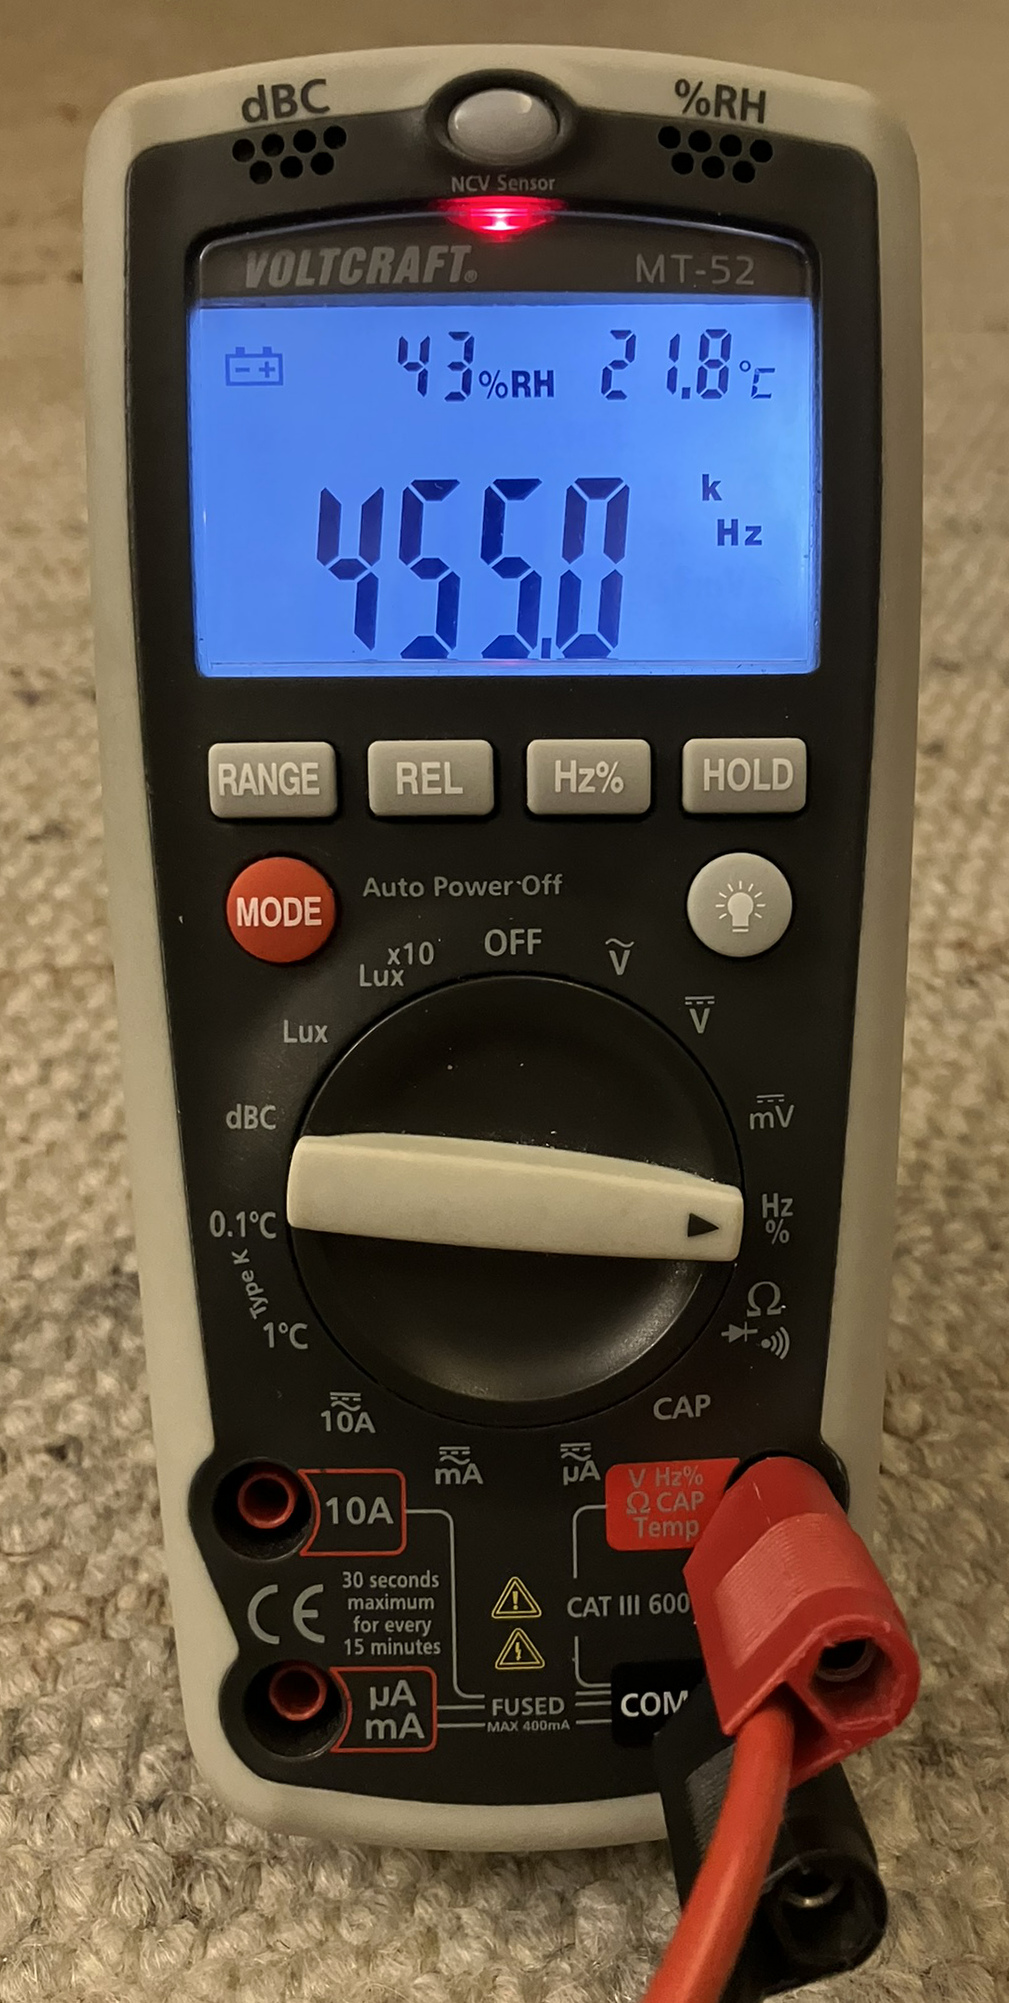
\includegraphics[width=0.85\textwidth]{foto/189}
    \caption{\scriptsize Multimeter, das im Frequenzmessbereich \qty{455}{\kilo\hertz} anzeigt. Darüber erscheinen ein Symbol für niedrige Batteriespannung, die Luftfeuchtigkeit und die Temperatur. Diese Werte haben nichts mit der Frequenzmessung zu tun.}
    \label{e_frequenzzaehler2}
\end{figure}

   \end{column}
\end{columns}

\end{frame}

\begin{frame}
\only<1>{
\begin{QQuestion}{EI501}{Womit kann die Frequenz eines unmodulierten Hochfrequenzsignals gemessen werden? Mit einem~...}{Frequenzzähler.}
{Widerstandsmessgerät.}
{Wechselspannungsmessgerät.}
{Wechselstromzähler.}
\end{QQuestion}

}
\only<2>{
\begin{QQuestion}{EI501}{Womit kann die Frequenz eines unmodulierten Hochfrequenzsignals gemessen werden? Mit einem~...}{\textbf{\textcolor{DARCgreen}{Frequenzzähler.}}}
{Widerstandsmessgerät.}
{Wechselspannungsmessgerät.}
{Wechselstromzähler.}
\end{QQuestion}

}
\end{frame}

\begin{frame}
\begin{columns}
    \begin{column}{0.48\textwidth}
    \begin{itemize}
  \item Anzeige der Frequenz
  \item Bei älteren Geräten steht hinten ein 10<sup>x</sup>-Multiplikator
  \end{itemize}

    \end{column}
   \begin{column}{0.48\textwidth}
       
\begin{figure}
    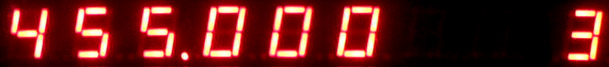
\includegraphics[width=0.85\textwidth]{foto/187}
    \caption{\scriptsize Display eines Frequenzzählers, der 455 · 10<sup>3</sup> Hz anzeigt}
    \label{e_frequenzzaehler1}
\end{figure}

   \end{column}
\end{columns}

\end{frame}

\begin{frame}
\begin{columns}
    \begin{column}{0.48\textwidth}
    \begin{itemize}
  \item Abgleichanleitung verlangt oft Einstellung bis auf eine bestimmte Abweichung
  \item z.B.  $\pm$ 10 Hz
  \item Stellenwert der Ziffern kennen
  \item Auf Komma und Einheitenpräfix oder Multiplikator achten
  \end{itemize}

    \end{column}
   \begin{column}{0.48\textwidth}
       
\begin{figure}
    \DARCimage{0.85\linewidth}{793include}
    \caption{\scriptsize Diese Anzeige stellt eine Frequenz in MHz dar. Das ist zugleich der Stellenwert der Ziffer vor dem Komma.}
    \label{e_frequenzzaehler_stellen}
\end{figure}


\begin{figure}
    \DARCimage{0.85\linewidth}{104include}
    \caption{\scriptsize Manche Anzeigen eines Frequenzzählers haben weniger Nachkommastellen}
    \label{e_frequenzzaehler_weniger_stellen}
\end{figure}


   \end{column}
\end{columns}

\end{frame}

\begin{frame}
\only<1>{
\begin{PQuestion}{EI502}{Das Bild stellt die Anzeige eines Frequenzzählers dar. Welchen Stellenwert hat die mit X gekennzeichnete Ziffer?}{ein Kilohertz}
{ein Hertz}
{hundert Hertz}
{zehn Hertz}
{\DARCimage{1.0\linewidth}{103include}}\end{PQuestion}

}
\only<2>{
\begin{PQuestion}{EI502}{Das Bild stellt die Anzeige eines Frequenzzählers dar. Welchen Stellenwert hat die mit X gekennzeichnete Ziffer?}{\textbf{\textcolor{DARCgreen}{ein Kilohertz}}}
{ein Hertz}
{hundert Hertz}
{zehn Hertz}
{\DARCimage{1.0\linewidth}{103include}}\end{PQuestion}

}
\end{frame}

\begin{frame}
\only<1>{
\begin{PQuestion}{EI503}{Das Bild stellt die Anzeige eines Frequenzzählers dar. Welchen Stellenwert hat die mit X gekennzeichnete Ziffer?}{ein Kilohertz}
{ein Hertz}
{hundert Hertz}
{zehn Hertz}
{\DARCimage{1.0\linewidth}{104include}}\end{PQuestion}

}
\only<2>{
\begin{PQuestion}{EI503}{Das Bild stellt die Anzeige eines Frequenzzählers dar. Welchen Stellenwert hat die mit X gekennzeichnete Ziffer?}{ein Kilohertz}
{ein Hertz}
{hundert Hertz}
{\textbf{\textcolor{DARCgreen}{zehn Hertz}}}
{\DARCimage{1.0\linewidth}{104include}}\end{PQuestion}

}
\end{frame}

\begin{frame}
\frametitle{Wertebereich}
\begin{itemize}
  \item Außerhalb des angegebenen Wertebereichs messen Frequenzzähler ungenau oder gar nicht
  \item Für höhere Frequenzen gibt es Frequenzteiler
  \item Angelegte Frequenz wird durch einen festen Wert geteilt
  \item Ergebnis wird als elektrische Schwingung ausgegeben
  \item \emph{Vorteiler} genannt, da zwischen Messobjekt und Zähler geschaltet
  \item 10:1-Teiler bei \qty{2,4}{\giga\hertz} $\rightarrow$ \qty{240}{\mega\hertz}
  \end{itemize}
\end{frame}

\begin{frame}
\only<1>{
\begin{QQuestion}{EI504}{Wenn ein 10:1-Frequenzteiler vor einem Frequenzzähler geschaltet wird und der Zähler \qty{14,5625}{\MHz} anzeigt, beträgt die tatsächliche Frequenz~...}{\qty{14,5625}{\kHz}.}
{\qty{1,45625}{\MHz}.}
{\qty{14,5625}{\MHz}.}
{\qty{145,625}{\MHz}.}
\end{QQuestion}

}
\only<2>{
\begin{QQuestion}{EI504}{Wenn ein 10:1-Frequenzteiler vor einem Frequenzzähler geschaltet wird und der Zähler \qty{14,5625}{\MHz} anzeigt, beträgt die tatsächliche Frequenz~...}{\qty{14,5625}{\kHz}.}
{\qty{1,45625}{\MHz}.}
{\qty{14,5625}{\MHz}.}
{\textbf{\textcolor{DARCgreen}{\qty{145,625}{\MHz}.}}}
\end{QQuestion}

}
\end{frame}%ENDCONTENT


\section{Frequenzmessung II}
\label{section:frequenzmessung_2}
\begin{frame}%STARTCONTENT

\only<1>{
\begin{QQuestion}{AI511}{Womit kann die Frequenzanzeige eines durchstimmbaren Empfängers möglichst genau geprüft werden?}{Mit einem LC-Oszillator hoher Schwingkreisgüte.}
{Mit einem Quarzofen- oder GPS-synchronisierten Frequenzgenerator.}
{Mit den Oberschwingungen eines konstant belasteten Schaltnetzteils.}
{Mit einem temperaturstabiliserten RC-Oszillator.}
\end{QQuestion}

}
\only<2>{
\begin{QQuestion}{AI511}{Womit kann die Frequenzanzeige eines durchstimmbaren Empfängers möglichst genau geprüft werden?}{Mit einem LC-Oszillator hoher Schwingkreisgüte.}
{\textbf{\textcolor{DARCgreen}{Mit einem Quarzofen- oder GPS-synchronisierten Frequenzgenerator.}}}
{Mit den Oberschwingungen eines konstant belasteten Schaltnetzteils.}
{Mit einem temperaturstabiliserten RC-Oszillator.}
\end{QQuestion}

}
\end{frame}

\begin{frame}
\only<1>{
\begin{QQuestion}{AI504}{Eine Frequenzmessung wird genauer, wenn bei einem Frequenzzähler~...}{ein Vorteiler mit höherem Teilverhältnis benutzt wird.}
{der Hauptoszillator temperaturstabilisiert wird.}
{die Messdauer möglichst kurz gehalten wird.}
{das Eingangssignal gleichgerichtet wird.}
\end{QQuestion}

}
\only<2>{
\begin{QQuestion}{AI504}{Eine Frequenzmessung wird genauer, wenn bei einem Frequenzzähler~...}{ein Vorteiler mit höherem Teilverhältnis benutzt wird.}
{\textbf{\textcolor{DARCgreen}{der Hauptoszillator temperaturstabilisiert wird.}}}
{die Messdauer möglichst kurz gehalten wird.}
{das Eingangssignal gleichgerichtet wird.}
\end{QQuestion}

}
\end{frame}

\begin{frame}
\only<1>{
\begin{QQuestion}{AI502}{Was kann man mit einem passenden Dämpfungsglied und einem Frequenzzähler messen?}{Die Sendefrequenz eines CW-Senders}
{Den Modulationsindex eines FM-Senders}
{Die Ausdehnung des Seitenbandes eines SSB-Senders}
{Den Frequenzhub eines FM-Senders}
\end{QQuestion}

}
\only<2>{
\begin{QQuestion}{AI502}{Was kann man mit einem passenden Dämpfungsglied und einem Frequenzzähler messen?}{\textbf{\textcolor{DARCgreen}{Die Sendefrequenz eines CW-Senders}}}
{Den Modulationsindex eines FM-Senders}
{Die Ausdehnung des Seitenbandes eines SSB-Senders}
{Den Frequenzhub eines FM-Senders}
\end{QQuestion}

}
\end{frame}

\begin{frame}
\only<1>{
\begin{QQuestion}{AI501}{Wenn die Frequenz eines Senders mit einem Frequenzzähler überprüft wird, ist~...}{der Zähler mit der Netzfrequenz zu synchronisieren.}
{ein Träger ohne Modulation zu verwenden.}
{der Zähler mit der Sendefrequenz zu synchronisieren.}
{eine analoge Modulation des Trägers zu verwenden.}
\end{QQuestion}

}
\only<2>{
\begin{QQuestion}{AI501}{Wenn die Frequenz eines Senders mit einem Frequenzzähler überprüft wird, ist~...}{der Zähler mit der Netzfrequenz zu synchronisieren.}
{\textbf{\textcolor{DARCgreen}{ein Träger ohne Modulation zu verwenden.}}}
{der Zähler mit der Sendefrequenz zu synchronisieren.}
{eine analoge Modulation des Trägers zu verwenden.}
\end{QQuestion}

}
\end{frame}

\begin{frame}
\only<1>{
\begin{QQuestion}{AI503}{Welche Konfiguration gewährleistet die höchste Genauigkeit bei der Prüfung der Trägerfrequenz eines FM-Senders?}{Absorptionsfrequenzmesser und modulierter Träger}
{Oszilloskop und unmodulierter Träger}
{Frequenzzähler und modulierter Träger}
{Frequenzzähler und unmodulierter Träger}
\end{QQuestion}

}
\only<2>{
\begin{QQuestion}{AI503}{Welche Konfiguration gewährleistet die höchste Genauigkeit bei der Prüfung der Trägerfrequenz eines FM-Senders?}{Absorptionsfrequenzmesser und modulierter Träger}
{Oszilloskop und unmodulierter Träger}
{Frequenzzähler und modulierter Träger}
{\textbf{\textcolor{DARCgreen}{Frequenzzähler und unmodulierter Träger}}}
\end{QQuestion}

}
\end{frame}

\begin{frame}
\only<1>{
\begin{QQuestion}{AI505}{Benutzt man bei einem Frequenzzähler eine Torzeit von 10 s anstelle von 1 s erhöht sich~...}{die Empfindlichkeit.}
{die Langzeitstabilität.}
{die Auflösung.}
{die Stabilität.}
\end{QQuestion}

}
\only<2>{
\begin{QQuestion}{AI505}{Benutzt man bei einem Frequenzzähler eine Torzeit von 10 s anstelle von 1 s erhöht sich~...}{die Empfindlichkeit.}
{die Langzeitstabilität.}
{\textbf{\textcolor{DARCgreen}{die Auflösung.}}}
{die Stabilität.}
\end{QQuestion}

}
\end{frame}%ENDCONTENT


\section{Frequenzgenauigkeit}
\label{section:frequenzgenauigkeit}
\begin{frame}%STARTCONTENT

\only<1>{
\begin{QQuestion}{AA115}{Eine Genauigkeit von \qty{1}{\ppm} bei einer Frequenz von \qty{435}{\MHz} entspricht~...}{\qty{43,5}{\Hz}.}
{\qty{435}{\Hz}.}
{\qty{4,35}{\MHz}.}
{\qty{4,35}{\kHz}.}
\end{QQuestion}

}
\only<2>{
\begin{QQuestion}{AA115}{Eine Genauigkeit von \qty{1}{\ppm} bei einer Frequenz von \qty{435}{\MHz} entspricht~...}{\qty{43,5}{\Hz}.}
{\textbf{\textcolor{DARCgreen}{\qty{435}{\Hz}.}}}
{\qty{4,35}{\MHz}.}
{\qty{4,35}{\kHz}.}
\end{QQuestion}

}
\end{frame}

\begin{frame}
\frametitle{Lösungsweg}
\begin{itemize}
  \item gegeben: $f = 435MHz$
  \item gesucht: $1pmm$ von $f$
  \end{itemize}
    \pause
    $435MHz \cdot frac{1}{10^6} = \frac{435\cdot \cancel{10^6}Hz}{\cancel{10^6}} = 435Hz$



\end{frame}

\begin{frame}
\only<1>{
\begin{QQuestion}{AA116}{Die Frequenzerzeugung eines Senders hat eine Genauigkeit von \qty{10}{\ppm}. Die digitale Anzeige zeigt eine Sendefrequenz von 14,200.\qty{000}{\MHz} an. In welchen Grenzen kann sich die tatsächliche Frequenz bewegen?}{Zwischen \qtyrange{14,199858}{14,200142}{\MHz}}
{Zwischen \qtyrange{14,199986}{14,200014}{\MHz}}
{Zwischen \qtyrange{14,199990}{14,200010}{\MHz}}
{Zwischen \qtyrange{14,198580}{14,201420}{\MHz}}
\end{QQuestion}

}
\only<2>{
\begin{QQuestion}{AA116}{Die Frequenzerzeugung eines Senders hat eine Genauigkeit von \qty{10}{\ppm}. Die digitale Anzeige zeigt eine Sendefrequenz von 14,200.\qty{000}{\MHz} an. In welchen Grenzen kann sich die tatsächliche Frequenz bewegen?}{\textbf{\textcolor{DARCgreen}{Zwischen \qtyrange{14,199858}{14,200142}{\MHz}}}}
{Zwischen \qtyrange{14,199986}{14,200014}{\MHz}}
{Zwischen \qtyrange{14,199990}{14,200010}{\MHz}}
{Zwischen \qtyrange{14,198580}{14,201420}{\MHz}}
\end{QQuestion}

}
\end{frame}

\begin{frame}
\frametitle{Lösungsweg}
\begin{itemize}
  \item gegeben: $f = 14,200.000MHz$
  \item gegeben: $\textrm{Abw.} = 10ppm$
  \item gesucht: $f_{min}, f_{max}$
  \end{itemize}
    \pause
    $f_{min} = f -- f \cdot \frac{10}{10^6} = 14,2MHz -- \frac{14,2\cdot \cancel{10^6}Hz\cdot 10}{\cancel{10^6}} = 14,2MHz -- 142Hz = 14,199858MHz$

$f_{max} = f + f \cdot \frac{10}{10^6} = 14,2MHz + \frac{14,2\cdot \cancel{10^6}Hz\cdot 10}{\cancel{10^6}} = 14,2MHz + 142Hz = 14,200142MHz$



\end{frame}

\begin{frame}
\only<1>{
\begin{QQuestion}{AI506}{Die relative Ungenauigkeit der digitalen Anzeige eines Empfängers beträgt \qty{0,01}{\percent}. Um wieviel Hertz kann die angezeigte Frequenz bei \qty{29}{\MHz} maximal abweichen?}{\qty{290}{\Hz}}
{\qty{2900}{\Hz}}
{\qty{29}{\Hz}}
{\qty{29}{\kHz}}
\end{QQuestion}

}
\only<2>{
\begin{QQuestion}{AI506}{Die relative Ungenauigkeit der digitalen Anzeige eines Empfängers beträgt \qty{0,01}{\percent}. Um wieviel Hertz kann die angezeigte Frequenz bei \qty{29}{\MHz} maximal abweichen?}{\qty{290}{\Hz}}
{\textbf{\textcolor{DARCgreen}{\qty{2900}{\Hz}}}}
{\qty{29}{\Hz}}
{\qty{29}{\kHz}}
\end{QQuestion}

}
\end{frame}

\begin{frame}
\frametitle{Lösungsweg}
\begin{itemize}
  \item gegeben: $f = 29MHz$
  \item gegeben: $\textrm{Abw.} = 0,01\%$
  \item gesucht: $\Delta f$
  \end{itemize}
    \pause
    $\Delta f = 29MHz \cdot 0,01\% = 29\cdot \cancel{10^6}Hz \cdot 100\cdot \cancel{10^{-6}} = 2900Hz$



\end{frame}

\begin{frame}
\only<1>{
\begin{QQuestion}{AI507}{Ein TRX mit einem eingebauten OCXO besitzt eine Anzeigegenauigkeit von $\pm$\qty{0,00001}{\percent}. Wie groß ist die maximale Abweichung, wenn eine Frequenz von \qty{14100}{\kHz} angezeigt wird?}{$\pm$ \qty{1,410}{\Hz}}
{$\pm$ \qty{0,141}{\Hz}}
{$\pm$ \qty{1,141}{\Hz}}
{$\pm$ \qty{114,1}{\Hz}}
\end{QQuestion}

}
\only<2>{
\begin{QQuestion}{AI507}{Ein TRX mit einem eingebauten OCXO besitzt eine Anzeigegenauigkeit von $\pm$\qty{0,00001}{\percent}. Wie groß ist die maximale Abweichung, wenn eine Frequenz von \qty{14100}{\kHz} angezeigt wird?}{\textbf{\textcolor{DARCgreen}{$\pm$ \qty{1,410}{\Hz}}}}
{$\pm$ \qty{0,141}{\Hz}}
{$\pm$ \qty{1,141}{\Hz}}
{$\pm$ \qty{114,1}{\Hz}}
\end{QQuestion}

}
\end{frame}

\begin{frame}
\frametitle{Lösungsweg}
\begin{itemize}
  \item gegeben: $f = 14100kHz$
  \item gegeben: $\textrm{Abw.} = \pm0,00001\%$
  \item gesucht: $\Delta f$
  \end{itemize}
    \pause
    $\Delta f = 14100kHz \cdot 0,00001\% = 14,1\cdot \cancel{10^6}Hz \cdot 0,1\cdot \cancel{10^{-6}} = 1,41Hz$



\end{frame}

\begin{frame}
\only<1>{
\begin{QQuestion}{AI508}{Ein Frequenzzähler misst auf $\pm$\qty{1}{\ppm} genau. Ist der Zähler auf den \qty{100}{\MHz}-Bereich eingestellt, so ist am oberen Ende dieses Bereiches eine Ungenauigkeit zu erwarten von~...}{$\pm$~\qty{1}{\Hz}.}
{$\pm$~\qty{10}{\Hz}.}
{$\pm$~\qty{1}{\kHz}.}
{$\pm$~\qty{100}{\Hz}.}
\end{QQuestion}

}
\only<2>{
\begin{QQuestion}{AI508}{Ein Frequenzzähler misst auf $\pm$\qty{1}{\ppm} genau. Ist der Zähler auf den \qty{100}{\MHz}-Bereich eingestellt, so ist am oberen Ende dieses Bereiches eine Ungenauigkeit zu erwarten von~...}{$\pm$~\qty{1}{\Hz}.}
{$\pm$~\qty{10}{\Hz}.}
{$\pm$~\qty{1}{\kHz}.}
{\textbf{\textcolor{DARCgreen}{$\pm$~\qty{100}{\Hz}.}}}
\end{QQuestion}

}
\end{frame}

\begin{frame}
\frametitle{Lösungsweg}
\begin{itemize}
  \item gegeben: $f = 100MHz$
  \item gegeben: $\textrm{Abw.} = \pm1ppm$
  \item gesucht: $\Delta f$
  \end{itemize}
    \pause
    $\Delta f = 100MHz \cdot \frac{1}{10^6} = \frac{100\cdot \cancel{10^6}Hz}{\cancel{10^6}} = 100Hz$



\end{frame}

\begin{frame}
\only<1>{
\begin{QQuestion}{AI509}{Mit einem auf \qty{10}{\ppm} genauen digitalen Frequenzzähler wird eine Frequenz von \qty{145}{\MHz} gemessen. In welchem Bereich liegt der vom Zähler angezeigte Frequenzwert?}{\qty{144,999275}{\MHz}~-~\qty{145,000725}{\MHz}}
{\qty{144,99565}{\MHz}~-~\qty{145,00435}{\MHz}}
{\qty{144,9971}{\MHz}~-~\qty{145,0029}{\MHz}}
{\qty{144,99855}{\MHz}~-~\qty{145,00145}{\MHz}}
\end{QQuestion}

}
\only<2>{
\begin{QQuestion}{AI509}{Mit einem auf \qty{10}{\ppm} genauen digitalen Frequenzzähler wird eine Frequenz von \qty{145}{\MHz} gemessen. In welchem Bereich liegt der vom Zähler angezeigte Frequenzwert?}{\qty{144,999275}{\MHz}~-~\qty{145,000725}{\MHz}}
{\qty{144,99565}{\MHz}~-~\qty{145,00435}{\MHz}}
{\qty{144,9971}{\MHz}~-~\qty{145,0029}{\MHz}}
{\textbf{\textcolor{DARCgreen}{\qty{144,99855}{\MHz}~-~\qty{145,00145}{\MHz}}}}
\end{QQuestion}

}
\end{frame}

\begin{frame}
\frametitle{Lösungsweg}
\begin{itemize}
  \item gegeben: $f = 145MHz$
  \item gegeben: $\textrm{Abw.} = 10ppm$
  \item gesucht: $f_{min},f_{max}$
  \end{itemize}
    \pause
    $\Delta f = 145MHz \cdot \frac{10}{10^6} = \frac{145\cdot \cancel{10^6}Hz \cdot 10}{\cancel{10^6}} = 1450Hz$
    \pause
    $f_{min} = f -- \Delta f = 145MHz -- 1450Hz = 144,99855MHz$

$f_{max} = f -- \Delta f = 145MHz + 1450Hz = 145,00145MHz$



\end{frame}

\begin{frame}
\only<1>{
\begin{QQuestion}{AI510}{Ein Transceivers zeigt Frequenzen im \qty{2}{\m}-Band auf \qty{1}{\ppm} genau an. Um wie viel kHz muss die an diesem Transceiver bei SSB-Betrieb (USB) eingestellte Sendefrequenz (Frequenz des unterdrückten Trägers) unterhalb von \qty{144,400}{\MHz} liegen, um das dort beginnende Bakensegment zu schützen, wenn die übertragene NF auf den Bereich \qty{300}{\Hz} bis \qty{2,7}{\kHz} beschränkt ist?}{\qty{0,144}{\kHz}}
{\qty{2,844}{\kHz}}
{\qty{1,42}{\kHz}}
{\qty{2,70}{\kHz}}
\end{QQuestion}

}
\only<2>{
\begin{QQuestion}{AI510}{Ein Transceivers zeigt Frequenzen im \qty{2}{\m}-Band auf \qty{1}{\ppm} genau an. Um wie viel kHz muss die an diesem Transceiver bei SSB-Betrieb (USB) eingestellte Sendefrequenz (Frequenz des unterdrückten Trägers) unterhalb von \qty{144,400}{\MHz} liegen, um das dort beginnende Bakensegment zu schützen, wenn die übertragene NF auf den Bereich \qty{300}{\Hz} bis \qty{2,7}{\kHz} beschränkt ist?}{\qty{0,144}{\kHz}}
{\textbf{\textcolor{DARCgreen}{\qty{2,844}{\kHz}}}}
{\qty{1,42}{\kHz}}
{\qty{2,70}{\kHz}}
\end{QQuestion}

}
\end{frame}

\begin{frame}
\frametitle{Lösungsweg}
\begin{itemize}
  \item gegeben: $f = 144,400MHz$
  \item gegeben: $\textrm{Abw.} = 1ppm$
  \item gegeben: $f_{B,max} = 2,7kHz$
  \item gesucht: $f_{B,max,Abw}$
  \end{itemize}
    \pause
    $\Delta f = 144,4MHz \cdot \frac{1}{10^6} = \frac{144,4\cdot \cancel{10^6}Hz}{\cancel{10^6}} = 144,4Hz$
    \pause
    $f_{B,max,Abw} = f_{B,max} + \Delta f = 2,7kHz + 144,4Hz = 2,8444kHz$



\end{frame}%ENDCONTENT


\title{DARC Amateurfunklehrgang Klasse NEA}
\author{Sender}
\institute{Deutscher Amateur Radio Club e.\,V.}
\begin{frame}
\maketitle
\end{frame}

\section{Aufbau eines Senders}
\label{section:aufbau_sender}
\begin{frame}%STARTCONTENT

\frametitle{1. Mikrofon}
\begin{columns}
    \begin{column}{0.48\textwidth}
    
\begin{figure}
    \DARCimage{0.85\linewidth}{735include}
    \caption{\scriptsize Blockdiagramm eines einfachen Senders}
    \label{aufbau_sender}
\end{figure}


    \end{column}
   \begin{column}{0.48\textwidth}
       \begin{itemize}
  \item Wandelt Schallwellen in NF-Signal um
  \end{itemize}

   \end{column}
\end{columns}

\end{frame}

\begin{frame}
\frametitle{2. Niederfrequenz-Verstärker}
\begin{columns}
    \begin{column}{0.48\textwidth}
    
\begin{figure}
    \DARCimage{0.85\linewidth}{735include}
    \caption{\scriptsize Blockdiagramm eines einfachen Senders}
    \label{aufbau_sender}
\end{figure}


    \end{column}
   \begin{column}{0.48\textwidth}
       \begin{itemize}
  \item Verstärkt das NF-Signal vom Mikrofon
  \end{itemize}

   \end{column}
\end{columns}

\end{frame}

\begin{frame}
\frametitle{3. Mischer}
\begin{columns}
    \begin{column}{0.48\textwidth}
    
\begin{figure}
    \DARCimage{0.85\linewidth}{735include}
    \caption{\scriptsize Blockdiagramm eines einfachen Senders}
    \label{aufbau_sender}
\end{figure}


    \end{column}
   \begin{column}{0.48\textwidth}
       \begin{itemize}
  \item Mischt das NF-Signal mit dem HF-Träger vom Oszillator (4)
  \end{itemize}

   \end{column}
\end{columns}

\end{frame}

\begin{frame}
\frametitle{4. Oszillator}
\begin{columns}
    \begin{column}{0.48\textwidth}
    
\begin{figure}
    \DARCimage{0.85\linewidth}{735include}
    \caption{\scriptsize Blockdiagramm eines einfachen Senders}
    \label{aufbau_sender}
\end{figure}


    \end{column}
   \begin{column}{0.48\textwidth}
       \begin{itemize}
  \item Erzeugt hochfrequente Schwingung der Sendefrequenz
  \end{itemize}

   \end{column}
\end{columns}

\end{frame}

\begin{frame}
\frametitle{5. Bandfilter}
\begin{columns}
    \begin{column}{0.48\textwidth}
    
\begin{figure}
    \DARCimage{0.85\linewidth}{735include}
    \caption{\scriptsize Blockdiagramm eines einfachen Senders}
    \label{aufbau_sender}
\end{figure}


    \end{column}
   \begin{column}{0.48\textwidth}
       \begin{itemize}
  \item Mischer erzeugt unerwünschte Frequenzen
  \item Mit dem Bandfilter werden nur die gewünschten Frequenzen durchgelassen
  \end{itemize}

   \end{column}
\end{columns}

\end{frame}

\begin{frame}
\frametitle{6. Verstärker}
\begin{columns}
    \begin{column}{0.48\textwidth}
    
\begin{figure}
    \DARCimage{0.85\linewidth}{735include}
    \caption{\scriptsize Blockdiagramm eines einfachen Senders}
    \label{aufbau_sender}
\end{figure}


    \end{column}
   \begin{column}{0.48\textwidth}
       \begin{itemize}
  \item Verstärkt das HF-Signal auf gewünschte Sendeleistung
  \end{itemize}

   \end{column}
\end{columns}

\end{frame}

\begin{frame}
\frametitle{7. Bandfilter}
\begin{columns}
    \begin{column}{0.48\textwidth}
    
\begin{figure}
    \DARCimage{0.85\linewidth}{735include}
    \caption{\scriptsize Blockdiagramm eines einfachen Senders}
    \label{aufbau_sender}
\end{figure}


    \end{column}
   \begin{column}{0.48\textwidth}
       \begin{itemize}
  \item Verstärker kann unerwünschte Frequenzen erzeugen
  \item Nur die gewünschten Frequenzen werden durchgelassen
  \end{itemize}

   \end{column}
\end{columns}

\end{frame}

\begin{frame}
\frametitle{8. Antenne}
\begin{columns}
    \begin{column}{0.48\textwidth}
    
\begin{figure}
    \DARCimage{0.85\linewidth}{735include}
    \caption{\scriptsize Blockdiagramm eines einfachen Senders}
    \label{aufbau_sender}
\end{figure}


    \end{column}
   \begin{column}{0.48\textwidth}
       \begin{itemize}
  \item HF-Signal wird auf Antenne gegeben
  \item Antenne strahlt es als Funkwelle ab
  \end{itemize}

   \end{column}
\end{columns}

\end{frame}

\begin{frame}
\only<1>{
\begin{PQuestion}{NF401}{Was stellt folgendes Blockdiagramm dar?}{Sender}
{Empfänger}
{Relaisfunkstelle}
{Antennenvorverstärker}
{\DARCimage{1.0\linewidth}{524include}}\end{PQuestion}

}
\only<2>{
\begin{PQuestion}{NF401}{Was stellt folgendes Blockdiagramm dar?}{\textbf{\textcolor{DARCgreen}{Sender}}}
{Empfänger}
{Relaisfunkstelle}
{Antennenvorverstärker}
{\DARCimage{1.0\linewidth}{524include}}\end{PQuestion}

}
\end{frame}

\begin{frame}
\only<1>{
\begin{PQuestion}{NF403}{Das nachfolgende Blockschaltbild zeigt einen einfachen Sender. An welcher Stelle befindet sich welche Stufe?}{1 HF-Verstärker; 
2 Filter; 
3 HF-Oszillator;  
4 NF-Verstärker; 
5 Mischer;
6 NF-Verstärker
}
{1 HF-Verstärker; 
2 Mischer; 
3 HF-Oszillator;  
4 Filter; 
5 NF-Verstärker; 
6 Filter
}
{1 NF-Verstärker; 
2 Filter; 
3 HF-Oszillator;  
4 Mischer; 
5 HF-Verstärker;
6 Mischer}
{1 NF-Verstärker; 
2 Mischer; 
3 HF-Oszillator;  
4 Filter; 
5 HF-Verstärker; 
6 Filter}
{\DARCimage{1.0\linewidth}{495include}}\end{PQuestion}

}
\only<2>{
\begin{PQuestion}{NF403}{Das nachfolgende Blockschaltbild zeigt einen einfachen Sender. An welcher Stelle befindet sich welche Stufe?}{1 HF-Verstärker; 
2 Filter; 
3 HF-Oszillator;  
4 NF-Verstärker; 
5 Mischer;
6 NF-Verstärker
}
{1 HF-Verstärker; 
2 Mischer; 
3 HF-Oszillator;  
4 Filter; 
5 NF-Verstärker; 
6 Filter
}
{1 NF-Verstärker; 
2 Filter; 
3 HF-Oszillator;  
4 Mischer; 
5 HF-Verstärker;
6 Mischer}
{\textbf{\textcolor{DARCgreen}{1 NF-Verstärker; 
2 Mischer; 
3 HF-Oszillator;  
4 Filter; 
5 HF-Verstärker; 
6 Filter}}}
{\DARCimage{1.0\linewidth}{495include}}\end{PQuestion}

}
\end{frame}

\begin{frame}
\only<1>{
\begin{QQuestion}{NF402}{Aus welchen Stufen besteht ein einfacher Sender?}{Vorverstärker, Filter, NF-Verstärker, Antenne}
{Vorverstärker, Filter, Demodulator, NF-Verstärker}
{Oszillator, Mischer, Filter, Leistungsverstärker}
{NF-Verstärker, Filter, Leistungsverstärker, Antenne}
\end{QQuestion}

}
\only<2>{
\begin{QQuestion}{NF402}{Aus welchen Stufen besteht ein einfacher Sender?}{Vorverstärker, Filter, NF-Verstärker, Antenne}
{Vorverstärker, Filter, Demodulator, NF-Verstärker}
{\textbf{\textcolor{DARCgreen}{Oszillator, Mischer, Filter, Leistungsverstärker}}}
{NF-Verstärker, Filter, Leistungsverstärker, Antenne}
\end{QQuestion}

}
\end{frame}

\begin{frame}Eine Amateurfunkanlage muss nach den allgemein anerkannten Regeln der Technik aufgebaut und betrieben werden. Das gilt natürlich auch ganz besonders für Sender.

\end{frame}

\begin{frame}
\only<1>{
\begin{QQuestion}{VD106}{Welche technischen Anforderungen stellt die Amateurfunkverordnung u.~a. an eine Amateurfunkstelle?}{Alle für den Sendebetrieb notwendigen Geräte müssen über ein CE-Zeichen verfügen.}
{Sie ist nach den allgemein anerkannten Regeln der Technik einzurichten und zu unterhalten.}
{Das Sendesignal muss über ein Koaxialkabel der Antenne zugeführt werden.}
{Sie darf bauartbedingt keine höhere Leistung erzeugen, als der Besitzer verwenden darf.}
\end{QQuestion}

}
\only<2>{
\begin{QQuestion}{VD106}{Welche technischen Anforderungen stellt die Amateurfunkverordnung u.~a. an eine Amateurfunkstelle?}{Alle für den Sendebetrieb notwendigen Geräte müssen über ein CE-Zeichen verfügen.}
{\textbf{\textcolor{DARCgreen}{Sie ist nach den allgemein anerkannten Regeln der Technik einzurichten und zu unterhalten.}}}
{Das Sendesignal muss über ein Koaxialkabel der Antenne zugeführt werden.}
{Sie darf bauartbedingt keine höhere Leistung erzeugen, als der Besitzer verwenden darf.}
\end{QQuestion}

}
\end{frame}%ENDCONTENT


\section{Modulatoren}
\label{section:modulatoren}
\begin{frame}%STARTCONTENT

\only<1>{
\begin{PQuestion}{AD503}{Bei dieser Schaltung ist der mit X bezeichnete Anschluss~...}{der Ausgang für das NF-Signal.}
{der Ausgang für eine Regelspannung.}
{der Ausgang für das Oszillatorsignal.}
{der Ausgang für das ZF-Signal.}
{\DARCimage{1.0\linewidth}{142include}}\end{PQuestion}

}
\only<2>{
\begin{PQuestion}{AD503}{Bei dieser Schaltung ist der mit X bezeichnete Anschluss~...}{der Ausgang für das NF-Signal.}
{\textbf{\textcolor{DARCgreen}{der Ausgang für eine Regelspannung.}}}
{der Ausgang für das Oszillatorsignal.}
{der Ausgang für das ZF-Signal.}
{\DARCimage{1.0\linewidth}{142include}}\end{PQuestion}

}
\end{frame}

\begin{frame}
\only<1>{
\begin{PQuestion}{AD507}{Bei dieser Schaltung handelt es sich um einen~...}{LSB-Modulator.}
{USB-Modulator.}
{FM-Modulator.}
{AM-Modulator.}
{\DARCimage{1.0\linewidth}{772include}}\end{PQuestion}

}
\only<2>{
\begin{PQuestion}{AD507}{Bei dieser Schaltung handelt es sich um einen~...}{LSB-Modulator.}
{USB-Modulator.}
{FM-Modulator.}
{\textbf{\textcolor{DARCgreen}{AM-Modulator.}}}
{\DARCimage{1.0\linewidth}{772include}}\end{PQuestion}

}
\end{frame}

\begin{frame}
\only<1>{
\begin{PQuestion}{AD508}{Bei dieser Schaltung handelt es sich um einen Modulator zur Erzeugung von~...}{AM-Signalen mit unterdrücktem Träger.}
{phasenmodulierten Signalen.}
{frequenzmodulierten Signalen.}
{AM-Signalen.}
{\DARCimage{1.0\linewidth}{155include}}\end{PQuestion}

}
\only<2>{
\begin{PQuestion}{AD508}{Bei dieser Schaltung handelt es sich um einen Modulator zur Erzeugung von~...}{AM-Signalen mit unterdrücktem Träger.}
{phasenmodulierten Signalen.}
{\textbf{\textcolor{DARCgreen}{frequenzmodulierten Signalen.}}}
{AM-Signalen.}
{\DARCimage{1.0\linewidth}{155include}}\end{PQuestion}

}
\end{frame}

\begin{frame}
\only<1>{
\begin{PQuestion}{AD509}{Was ermöglicht die abgebildete Schaltung?}{Die Erzeugung von Phasenmodulation}
{Die HF-Pegelbegrenzung und HF-Pegeleinstellung bei FM-Funkgeräten}
{Die Erzeugung von Amplitudenmodulation}
{Die Hubbegrenzung und Hubeinstellung bei FM-Funkgeräten}
{\DARCimage{1.0\linewidth}{44include}}\end{PQuestion}

}
\only<2>{
\begin{PQuestion}{AD509}{Was ermöglicht die abgebildete Schaltung?}{Die Erzeugung von Phasenmodulation}
{Die HF-Pegelbegrenzung und HF-Pegeleinstellung bei FM-Funkgeräten}
{Die Erzeugung von Amplitudenmodulation}
{\textbf{\textcolor{DARCgreen}{Die Hubbegrenzung und Hubeinstellung bei FM-Funkgeräten}}}
{\DARCimage{1.0\linewidth}{44include}}\end{PQuestion}

}
\end{frame}

\begin{frame}
\only<1>{
\begin{QQuestion}{AE206}{Welche Baugruppe sollte für die analoge Erzeugung eines unterdrückten Zweiseitenband-Trägersignals verwendet werden?}{Demodulator}
{Quarzfilter}
{Bandfilter}
{Balancemischer}
\end{QQuestion}

}
\only<2>{
\begin{QQuestion}{AE206}{Welche Baugruppe sollte für die analoge Erzeugung eines unterdrückten Zweiseitenband-Trägersignals verwendet werden?}{Demodulator}
{Quarzfilter}
{Bandfilter}
{\textbf{\textcolor{DARCgreen}{Balancemischer}}}
\end{QQuestion}

}
\end{frame}

\begin{frame}
\only<1>{
\begin{QQuestion}{AF302}{Welcher Mischertyp ist am besten geeignet, um ein Doppelseitenbandsignal mit unterdrücktem Träger zu erzeugen?}{Ein Mischer mit einem einzelnen FET}
{Ein Balancemischer}
{Ein Mischer mit einer Varaktordiode}
{Ein quarzgesteuerter Mischer}
\end{QQuestion}

}
\only<2>{
\begin{QQuestion}{AF302}{Welcher Mischertyp ist am besten geeignet, um ein Doppelseitenbandsignal mit unterdrücktem Träger zu erzeugen?}{Ein Mischer mit einem einzelnen FET}
{\textbf{\textcolor{DARCgreen}{Ein Balancemischer}}}
{Ein Mischer mit einer Varaktordiode}
{Ein quarzgesteuerter Mischer}
\end{QQuestion}

}
\end{frame}

\begin{frame}
\only<1>{
\begin{QQuestion}{AF303}{Wie kann mit analoger Technologie ein SSB-Signal erzeugt werden?}{In einem Balancemodulator wird ein Zweiseitenband-Signal erzeugt. Das Seitenbandfilter selektiert ein Seitenband heraus.}
{In einem Balancemodulator wird ein Zweiseitenband-Signal erzeugt. Ein auf die Trägerfrequenz abgestimmter Saugkreis filtert den Träger aus.}
{In einem Balancemodulator wird ein Zweiseitenband-Signal erzeugt. Ein auf die Trägerfrequenz abgestimmter Sperrkreis filtert den Träger aus.}
{In einem Balancemodulator wird ein Zweiseitenband-Signal erzeugt. In einem Frequenzteiler wird ein Seitenband abgespalten.}
\end{QQuestion}

}
\only<2>{
\begin{QQuestion}{AF303}{Wie kann mit analoger Technologie ein SSB-Signal erzeugt werden?}{\textbf{\textcolor{DARCgreen}{In einem Balancemodulator wird ein Zweiseitenband-Signal erzeugt. Das Seitenbandfilter selektiert ein Seitenband heraus.}}}
{In einem Balancemodulator wird ein Zweiseitenband-Signal erzeugt. Ein auf die Trägerfrequenz abgestimmter Saugkreis filtert den Träger aus.}
{In einem Balancemodulator wird ein Zweiseitenband-Signal erzeugt. Ein auf die Trägerfrequenz abgestimmter Sperrkreis filtert den Träger aus.}
{In einem Balancemodulator wird ein Zweiseitenband-Signal erzeugt. In einem Frequenzteiler wird ein Seitenband abgespalten.}
\end{QQuestion}

}
\end{frame}

\begin{frame}
\only<1>{
\begin{QQuestion}{AF304}{Bei üblichen analogen Methoden zur Aufbereitung eines SSB-Signals werden~...}{der Träger unterdrückt und ein Seitenband hinzugesetzt.}
{der Träger hinzugesetzt und ein Seitenband ausgefiltert.}
{der Träger unterdrückt und ein Seitenband ausgefiltert.}
{der Träger unterdrückt und beide Seitenbänder ausgefiltert.}
\end{QQuestion}

}
\only<2>{
\begin{QQuestion}{AF304}{Bei üblichen analogen Methoden zur Aufbereitung eines SSB-Signals werden~...}{der Träger unterdrückt und ein Seitenband hinzugesetzt.}
{der Träger hinzugesetzt und ein Seitenband ausgefiltert.}
{\textbf{\textcolor{DARCgreen}{der Träger unterdrückt und ein Seitenband ausgefiltert.}}}
{der Träger unterdrückt und beide Seitenbänder ausgefiltert.}
\end{QQuestion}

}
\end{frame}

\begin{frame}
\only<1>{
\begin{PQuestion}{AF305}{Dieses Blockschaltbild zeigt einen SSB-Sender. Die Stufe bei \glqq?\grqq{} ist ein...}{ZF-Notchfilter zur Unterdrückung des unerwünschten Seitenbands.}
{RC-Hochpass zur Unterdrückung des unteren Seitenbands.}
{RL-Tiefpass zur Unterdrückung des oberen Seitenbands.}
{Quarzfilter als Bandpass für das gewünschte Seitenband.}
{\DARCimage{1.0\linewidth}{98include}}\end{PQuestion}

}
\only<2>{
\begin{PQuestion}{AF305}{Dieses Blockschaltbild zeigt einen SSB-Sender. Die Stufe bei \glqq?\grqq{} ist ein...}{ZF-Notchfilter zur Unterdrückung des unerwünschten Seitenbands.}
{RC-Hochpass zur Unterdrückung des unteren Seitenbands.}
{RL-Tiefpass zur Unterdrückung des oberen Seitenbands.}
{\textbf{\textcolor{DARCgreen}{Quarzfilter als Bandpass für das gewünschte Seitenband.}}}
{\DARCimage{1.0\linewidth}{98include}}\end{PQuestion}

}
\end{frame}

\begin{frame}
\only<1>{
\begin{PQuestion}{AF306}{Welches Schaltungsteil ist in der folgenden Blockschaltung am Ausgang des NF-Verstärkers angeschlossen?}{symmetrisches Filter}
{Balancemischer}
{Dynamikkompressor}
{DSB-Filter}
{\DARCimage{1.0\linewidth}{500include}}\end{PQuestion}

}
\only<2>{
\begin{PQuestion}{AF306}{Welches Schaltungsteil ist in der folgenden Blockschaltung am Ausgang des NF-Verstärkers angeschlossen?}{symmetrisches Filter}
{\textbf{\textcolor{DARCgreen}{Balancemischer}}}
{Dynamikkompressor}
{DSB-Filter}
{\DARCimage{1.0\linewidth}{500include}}\end{PQuestion}

}
\end{frame}

\begin{frame}
\only<1>{
\begin{PQuestion}{AF307}{Die folgende Blockschaltung zeigt eine SSB-Aufbereitung mit einem \qty{9}{\MHz}-Quarzfilter. Welche Frequenz wird in der Schalterstellung USB mit der NF gemischt?}{\qty{9,0000}{\MHz}}
{\qty{8,9970}{\MHz}}
{\qty{8,9985}{\MHz}}
{\qty{9,0030}{\MHz}}
{\DARCimage{1.0\linewidth}{39include}}\end{PQuestion}

}
\only<2>{
\begin{PQuestion}{AF307}{Die folgende Blockschaltung zeigt eine SSB-Aufbereitung mit einem \qty{9}{\MHz}-Quarzfilter. Welche Frequenz wird in der Schalterstellung USB mit der NF gemischt?}{\qty{9,0000}{\MHz}}
{\qty{8,9970}{\MHz}}
{\textbf{\textcolor{DARCgreen}{\qty{8,9985}{\MHz}}}}
{\qty{9,0030}{\MHz}}
{\DARCimage{1.0\linewidth}{39include}}\end{PQuestion}

}
\end{frame}

\begin{frame}
\frametitle{Lösungsweg}
\begin{itemize}
  \item gegeben: $f_Q = 9MHz$
  \item gegeben: $f_{LSB} = 9,0015MHz$
  \item gesucht: $f_{USB}$
  \end{itemize}
    \pause
    $f_{USB} = f_Q -- (f_{LSB} -- f_Q) = 9MHz -- (9,0015MHz -- 9MHz) = 9MHz -- 0,0015MHz =8,9985MHz$



\end{frame}

\begin{frame}
\only<1>{
\begin{PQuestion}{AF308}{Bei dieser Schaltung handelt es sich um einen Modulator zur Erzeugung von~...}{AM-Signalen mit unterdrücktem Träger.}
{phasenmodulierten Signalen.}
{frequenzmodulierten Signalen.}
{LSB-Signalen.}
{\DARCimage{1.0\linewidth}{759include}}\end{PQuestion}

}
\only<2>{
\begin{PQuestion}{AF308}{Bei dieser Schaltung handelt es sich um einen Modulator zur Erzeugung von~...}{\textbf{\textcolor{DARCgreen}{AM-Signalen mit unterdrücktem Träger.}}}
{phasenmodulierten Signalen.}
{frequenzmodulierten Signalen.}
{LSB-Signalen.}
{\DARCimage{1.0\linewidth}{759include}}\end{PQuestion}

}
\end{frame}

\begin{frame}
\only<1>{
\begin{PQuestion}{AF309}{Wozu dienen $R_1$ und $C_1$ bei dieser Schaltung?  }{Sie dienen zur Einstellung des Modulationsgrades des erzeugten DSB-Signals.}
{Sie dienen zum Ausgleich von Frequenzgangs- und Laufzeitunterschieden.}
{Sie dienen zur Einstellung des Frequenzhubes mit Hilfe der ersten Trägernullstelle.}
{Sie dienen zur Einstellung der Trägerunterdrückung nach Betrag und Phase.}
{\DARCimage{1.0\linewidth}{762include}}\end{PQuestion}

}
\only<2>{
\begin{PQuestion}{AF309}{Wozu dienen $R_1$ und $C_1$ bei dieser Schaltung?  }{Sie dienen zur Einstellung des Modulationsgrades des erzeugten DSB-Signals.}
{Sie dienen zum Ausgleich von Frequenzgangs- und Laufzeitunterschieden.}
{Sie dienen zur Einstellung des Frequenzhubes mit Hilfe der ersten Trägernullstelle.}
{\textbf{\textcolor{DARCgreen}{Sie dienen zur Einstellung der Trägerunterdrückung nach Betrag und Phase.}}}
{\DARCimage{1.0\linewidth}{762include}}\end{PQuestion}

}
\end{frame}

\begin{frame}
\only<1>{
\begin{PQuestion}{AF310}{Dieser Schaltungsauszug ist Teil eines Senders. Welche Funktion hat die Diode?}{Sie stabilisiert die Betriebsspannung für den Oszillator, um diesen von der Stromversorgung der anderen Stufen zu entkoppeln.}
{Sie beeinflusst die Resonanzfrequenz des Schwingkreises in Abhängigkeit des NF-Spannungsverlaufs und moduliert so die Oszillatorfrequenz.}
{Sie begrenzt die Amplituden des Eingangssignals und vermeidet so die Übersteuerung der Oszillatorstufe.}
{Sie dient zur Erzeugung von Amplitudenmodulation in Abhängigkeit von den Frequenzen im Basisband.}
{\DARCimage{1.0\linewidth}{158include}}\end{PQuestion}

}
\only<2>{
\begin{PQuestion}{AF310}{Dieser Schaltungsauszug ist Teil eines Senders. Welche Funktion hat die Diode?}{Sie stabilisiert die Betriebsspannung für den Oszillator, um diesen von der Stromversorgung der anderen Stufen zu entkoppeln.}
{\textbf{\textcolor{DARCgreen}{Sie beeinflusst die Resonanzfrequenz des Schwingkreises in Abhängigkeit des NF-Spannungsverlaufs und moduliert so die Oszillatorfrequenz.}}}
{Sie begrenzt die Amplituden des Eingangssignals und vermeidet so die Übersteuerung der Oszillatorstufe.}
{Sie dient zur Erzeugung von Amplitudenmodulation in Abhängigkeit von den Frequenzen im Basisband.}
{\DARCimage{1.0\linewidth}{158include}}\end{PQuestion}

}
\end{frame}

\begin{frame}
\only<1>{
\begin{QQuestion}{AD510}{Welche Signale stehen am Ausgang eines symmetrisch eingestellten Balancemischers an?}{Der vollständige Träger}
{Viele Mischprodukte}
{Der verringerte Träger und ein Seitenband}
{Die zwei Seitenbänder}
\end{QQuestion}

}
\only<2>{
\begin{QQuestion}{AD510}{Welche Signale stehen am Ausgang eines symmetrisch eingestellten Balancemischers an?}{Der vollständige Träger}
{Viele Mischprodukte}
{Der verringerte Träger und ein Seitenband}
{\textbf{\textcolor{DARCgreen}{Die zwei Seitenbänder}}}
\end{QQuestion}

}
\end{frame}%ENDCONTENT


\section{Nicht-sinusförmige Signale}
\label{section:nicht_sinus_signale}
\begin{frame}%STARTCONTENT

\only<1>{
\begin{PQuestion}{AB403}{Eine periodische Schwingung, die wie das folgende Signal aussieht, besteht~...}{aus der Grundschwingung mit ganzzahligen Vielfachen dieser Frequenz (Oberschwingungen).}
{aus der Grundschwingung und Teilen dieser Frequenz (Unterschwingungen).}
{aus der Grundschwingung ohne weitere Frequenzen.}
{aus der Grundschwingung mit zufälligen Frequenzschwankungen.}
{\DARCimage{1.0\linewidth}{595include}}\end{PQuestion}

}
\only<2>{
\begin{PQuestion}{AB403}{Eine periodische Schwingung, die wie das folgende Signal aussieht, besteht~...}{\textbf{\textcolor{DARCgreen}{aus der Grundschwingung mit ganzzahligen Vielfachen dieser Frequenz (Oberschwingungen).}}}
{aus der Grundschwingung und Teilen dieser Frequenz (Unterschwingungen).}
{aus der Grundschwingung ohne weitere Frequenzen.}
{aus der Grundschwingung mit zufälligen Frequenzschwankungen.}
{\DARCimage{1.0\linewidth}{595include}}\end{PQuestion}

}
\end{frame}

\begin{frame}
\only<1>{
\begin{QQuestion}{AB401}{Was sind Harmonische?}{Harmonische sind ausschließlich die ungeradzahligen (1, 3, 5,~...) Vielfachen einer Frequenz.}
{Harmonische sind die ganzzahligen (1, 2, 3,~...) Teile einer Frequenz.}
{Harmonische sind die ganzzahligen (1, 2, 3,~...) Vielfachen einer Frequenz.}
{Harmonische sind ausschließlich die geradzahligen (2, 4, 6,~...) Teile einer Frequenz.}
\end{QQuestion}

}
\only<2>{
\begin{QQuestion}{AB401}{Was sind Harmonische?}{Harmonische sind ausschließlich die ungeradzahligen (1, 3, 5,~...) Vielfachen einer Frequenz.}
{Harmonische sind die ganzzahligen (1, 2, 3,~...) Teile einer Frequenz.}
{\textbf{\textcolor{DARCgreen}{Harmonische sind die ganzzahligen (1, 2, 3,~...) Vielfachen einer Frequenz.}}}
{Harmonische sind ausschließlich die geradzahligen (2, 4, 6,~...) Teile einer Frequenz.}
\end{QQuestion}

}
\end{frame}

\begin{frame}
\only<1>{
\begin{QQuestion}{AB402}{Die dritte Oberwelle entspricht~...}{der dritten Harmonischen.}
{der vierten Harmonischen.}
{der zweiten Harmonischen.}
{der zweiten ungeradzahligen Harmonischen.}
\end{QQuestion}

}
\only<2>{
\begin{QQuestion}{AB402}{Die dritte Oberwelle entspricht~...}{der dritten Harmonischen.}
{\textbf{\textcolor{DARCgreen}{der vierten Harmonischen.}}}
{der zweiten Harmonischen.}
{der zweiten ungeradzahligen Harmonischen.}
\end{QQuestion}

}
\end{frame}

\begin{frame}
\only<1>{
\begin{QQuestion}{AI615}{Mit welchem Messgerät kann man das Vorhandensein von Harmonischen nachweisen?}{Spektrumanalysator}
{Stehwellenmessgerät}
{Vektorieller Netzwerkanalysator (VNA)}
{Frequenzzähler}
\end{QQuestion}

}
\only<2>{
\begin{QQuestion}{AI615}{Mit welchem Messgerät kann man das Vorhandensein von Harmonischen nachweisen?}{\textbf{\textcolor{DARCgreen}{Spektrumanalysator}}}
{Stehwellenmessgerät}
{Vektorieller Netzwerkanalysator (VNA)}
{Frequenzzähler}
\end{QQuestion}

}
\end{frame}

\begin{frame}
\only<1>{
\begin{QQuestion}{AI614}{Mit welchem der folgenden Messinstrumente können die Amplituden der Harmonischen eines Signals gemessen werden? Sie können gemessen werden mit einem~...}{Breitbandpegelmesser.}
{Frequenzzähler.}
{Spektrumanalysator.}
{Multimeter.}
\end{QQuestion}

}
\only<2>{
\begin{QQuestion}{AI614}{Mit welchem der folgenden Messinstrumente können die Amplituden der Harmonischen eines Signals gemessen werden? Sie können gemessen werden mit einem~...}{Breitbandpegelmesser.}
{Frequenzzähler.}
{\textbf{\textcolor{DARCgreen}{Spektrumanalysator.}}}
{Multimeter.}
\end{QQuestion}

}
\end{frame}

\begin{frame}
\only<1>{
\begin{QQuestion}{AJ201}{Die zweite Harmonische der Frequenz \qty{3,730}{\MHz} befindet sich auf~...}{\qty{11,190}{\MHz}.}
{\qty{1,865}{\MHz}.}
{\qty{7,460}{\MHz}.}
{\qty{5,730}{\MHz}.}
\end{QQuestion}

}
\only<2>{
\begin{QQuestion}{AJ201}{Die zweite Harmonische der Frequenz \qty{3,730}{\MHz} befindet sich auf~...}{\qty{11,190}{\MHz}.}
{\qty{1,865}{\MHz}.}
{\textbf{\textcolor{DARCgreen}{\qty{7,460}{\MHz}.}}}
{\qty{5,730}{\MHz}.}
\end{QQuestion}

}
\end{frame}

\begin{frame}
\frametitle{Lösungsweg}
\begin{itemize}
  \item gegeben: $f = 3,730MHz$
  \item gesucht: $f$ der 2. Harmonischen
  \end{itemize}
    \pause
    $2 \cdot f = 2 \cdot 3,730MHz = 7,460MHz$



\end{frame}

\begin{frame}
\only<1>{
\begin{QQuestion}{AJ205}{Die zweite ungeradzahlige Harmonische der Frequenz \qty{144,690}{\MHz} ist~...}{\qty{723,450}{\MHz}.}
{\qty{289,380}{\MHz}.}
{\qty{145,000}{\MHz}.}
{\qty{434,070}{\MHz}.}
\end{QQuestion}

}
\only<2>{
\begin{QQuestion}{AJ205}{Die zweite ungeradzahlige Harmonische der Frequenz \qty{144,690}{\MHz} ist~...}{\qty{723,450}{\MHz}.}
{\qty{289,380}{\MHz}.}
{\qty{145,000}{\MHz}.}
{\textbf{\textcolor{DARCgreen}{\qty{434,070}{\MHz}.}}}
\end{QQuestion}

}
\end{frame}

\begin{frame}
\frametitle{Lösungsweg}
\begin{itemize}
  \item gegeben: $f = 144,690MHz$
  \item gesucht: $f$ als 2. ungeradzahlige Harmonische
  \end{itemize}
    \pause
    \begin{enumerate}
  \item[2] ungeradzahlige Harmonische = 3. Harmonische
  \end{enumerate}
$3 \cdot f = 3 \cdot 144,690MHz = 434,070MHz$



\end{frame}

\begin{frame}
\only<1>{
\begin{QQuestion}{AJ202}{Auf welche Frequenz müsste ein Empfänger eingestellt werden, um die dritte Harmonische einer nahen \qty{7,050}{\MHz}-Aussendung erkennen zu können?}{\qty{21,150}{\MHz}}
{\qty{14,100}{\MHz}}
{\qty{35,250}{\MHz}}
{\qty{28,200}{\MHz}}
\end{QQuestion}

}
\only<2>{
\begin{QQuestion}{AJ202}{Auf welche Frequenz müsste ein Empfänger eingestellt werden, um die dritte Harmonische einer nahen \qty{7,050}{\MHz}-Aussendung erkennen zu können?}{\textbf{\textcolor{DARCgreen}{\qty{21,150}{\MHz}}}}
{\qty{14,100}{\MHz}}
{\qty{35,250}{\MHz}}
{\qty{28,200}{\MHz}}
\end{QQuestion}

}
\end{frame}

\begin{frame}
\frametitle{Lösungsweg}
\begin{itemize}
  \item gegeben: $f = 7,050MHz$
  \item gesucht: $f$ als 3. Harmonische
  \end{itemize}
    \pause
    $3 \cdot f = 3 \cdot 7,050MHz = 21,150MHz$



\end{frame}

\begin{frame}
\only<1>{
\begin{QQuestion}{AJ206}{Auf welchen Frequenzen kann ein \qty{144,300}{\MHz} SSB-Sendesignal Störungen verursachen?}{\qty{432,900}{\MHz} und \qty{1298,700}{\MHz}}
{\qty{433,900}{\MHz} und \qty{1296,700}{\MHz}}
{\qty{438,900}{\MHz} und \qty{1290,700}{\MHz}}
{\qty{434,900}{\MHz} und \qty{1298,700}{\MHz}}
\end{QQuestion}

}
\only<2>{
\begin{QQuestion}{AJ206}{Auf welchen Frequenzen kann ein \qty{144,300}{\MHz} SSB-Sendesignal Störungen verursachen?}{\textbf{\textcolor{DARCgreen}{\qty{432,900}{\MHz} und \qty{1298,700}{\MHz}}}}
{\qty{433,900}{\MHz} und \qty{1296,700}{\MHz}}
{\qty{438,900}{\MHz} und \qty{1290,700}{\MHz}}
{\qty{434,900}{\MHz} und \qty{1298,700}{\MHz}}
\end{QQuestion}

}
\end{frame}

\begin{frame}
\frametitle{Lösungsweg}
\begin{itemize}
  \item gegeben: $f = 144,300MHz$
  \item gesucht: mehrere Harmonische
  \end{itemize}
    \pause
    $$\begin{align}\notag 2 \cdot 144,300MHz &= 288,600MHz\\ \notag 3 \cdot 144,300MHz &= \bold{432,900MHz}\\ \notag &\vdots\\ \notag 9 \cdot 144,300MHz &= \bold{1298,700MHz}\end{align}$$



\end{frame}%ENDCONTENT


\section{Leistungsverstärker}
\label{section:leistungsvertaerker}
\begin{frame}%STARTCONTENT

\only<1>{
\begin{PQuestion}{AF412}{Welche Art von Schaltung wird im folgenden Bild dargestellt? Es handelt sich um einen~...}{modulierbaren Oszillator.}
{selektiven Hochfrequenzverstärker.}
{Breitband-Gegentaktverstärker.}
{Breitband-Frequenzverdoppler.}
{\DARCimage{1.0\linewidth}{491include}}\end{PQuestion}

}
\only<2>{
\begin{PQuestion}{AF412}{Welche Art von Schaltung wird im folgenden Bild dargestellt? Es handelt sich um einen~...}{modulierbaren Oszillator.}
{selektiven Hochfrequenzverstärker.}
{\textbf{\textcolor{DARCgreen}{Breitband-Gegentaktverstärker.}}}
{Breitband-Frequenzverdoppler.}
{\DARCimage{1.0\linewidth}{491include}}\end{PQuestion}

}
\end{frame}

\begin{frame}
\only<1>{
\begin{PQuestion}{AF408}{Worum handelt es sich bei dieser Schaltung?}{Es handelt sich um einen selektiven HF-Verstärker.}
{Es handelt sich um einen selektiven Mischer.}
{Es handelt sich um einen breitbandigen NF-Verstärker.}
{Es handelt sich um einen frequenzvervielfachenden Oszillator.}
{\DARCimage{1.0\linewidth}{778include}}\end{PQuestion}

}
\only<2>{
\begin{PQuestion}{AF408}{Worum handelt es sich bei dieser Schaltung?}{\textbf{\textcolor{DARCgreen}{Es handelt sich um einen selektiven HF-Verstärker.}}}
{Es handelt sich um einen selektiven Mischer.}
{Es handelt sich um einen breitbandigen NF-Verstärker.}
{Es handelt sich um einen frequenzvervielfachenden Oszillator.}
{\DARCimage{1.0\linewidth}{778include}}\end{PQuestion}

}
\end{frame}

\begin{frame}
\only<1>{
\begin{PQuestion}{AF413}{Worum handelt es sich bei dieser Schaltung? Es handelt sich um einen...}{zweistufigen Breitband-HF-Verstärker.}
{selektiven Hochfrequenzverstärker.}
{Gegentakt-Verstärker im B-Betrieb.}
{zweistufigen LC-Oszillator.}
{\DARCimage{1.0\linewidth}{764include}}\end{PQuestion}

}
\only<2>{
\begin{PQuestion}{AF413}{Worum handelt es sich bei dieser Schaltung? Es handelt sich um einen...}{\textbf{\textcolor{DARCgreen}{zweistufigen Breitband-HF-Verstärker.}}}
{selektiven Hochfrequenzverstärker.}
{Gegentakt-Verstärker im B-Betrieb.}
{zweistufigen LC-Oszillator.}
{\DARCimage{1.0\linewidth}{764include}}\end{PQuestion}

}
\end{frame}

\begin{frame}
\only<1>{
\begin{PQuestion}{AF409}{Welchem Zweck dient die Anzapfung an X in der folgenden Schaltung?}{Sie bewirkt die notwendige Entkopplung für den Schwingungseinsatz der Oszillatorstufe.}
{Sie ermöglicht die Dreipunkt-Rückkopplung des Oszillators.}
{Sie dient zur Anpassung der Eingangsimpedanz dieser Stufe an die vorgelagerte Stufe.}
{Sie bewirkt eine stärkere Bedämpfung des Eingangsschwingkreises.}
{\DARCimage{1.0\linewidth}{779include}}\end{PQuestion}

}
\only<2>{
\begin{PQuestion}{AF409}{Welchem Zweck dient die Anzapfung an X in der folgenden Schaltung?}{Sie bewirkt die notwendige Entkopplung für den Schwingungseinsatz der Oszillatorstufe.}
{Sie ermöglicht die Dreipunkt-Rückkopplung des Oszillators.}
{\textbf{\textcolor{DARCgreen}{Sie dient zur Anpassung der Eingangsimpedanz dieser Stufe an die vorgelagerte Stufe.}}}
{Sie bewirkt eine stärkere Bedämpfung des Eingangsschwingkreises.}
{\DARCimage{1.0\linewidth}{779include}}\end{PQuestion}

}
\end{frame}

\begin{frame}
\only<1>{
\begin{PQuestion}{AF410}{Welchem Zweck dienen $C_1$ und $C_2$ in der folgenden Schaltung? Sie dienen zur...}{Impedanzanpassung. }
{Verhinderung der Schwingneigung.}
{Realisierung einer kapazitiven Dreipunktschaltung für den Oszillator.}
{Unterdrückung von Oberschwingungen.}
{\DARCimage{1.0\linewidth}{780include}}\end{PQuestion}

}
\only<2>{
\begin{PQuestion}{AF410}{Welchem Zweck dienen $C_1$ und $C_2$ in der folgenden Schaltung? Sie dienen zur...}{\textbf{\textcolor{DARCgreen}{Impedanzanpassung. }}}
{Verhinderung der Schwingneigung.}
{Realisierung einer kapazitiven Dreipunktschaltung für den Oszillator.}
{Unterdrückung von Oberschwingungen.}
{\DARCimage{1.0\linewidth}{780include}}\end{PQuestion}

}
\end{frame}

\begin{frame}
\only<1>{
\begin{PQuestion}{AF414}{Wozu dient der Transformator $T_1$ der folgenden Schaltung?}{Er dient der Anpassung des Ausgangswiderstandes der Emitterschaltung an den Eingang der folgenden Emitterschaltung.}
{Er dient der Anpassung des Ausgangswiderstandes der Emitterschaltung an den Eingang der folgenden Kollektorschaltung.}
{Er dient der Anpassung des Ausgangswiderstandes der Kollektorschaltung an den Eingang der folgenden Emitterschaltung.}
{Er dient der Anpassung des Ausgangswiderstandes der Kollektorschaltung an den Eingang der folgenden PA.}
{\DARCimage{1.0\linewidth}{765include}}\end{PQuestion}

}
\only<2>{
\begin{PQuestion}{AF414}{Wozu dient der Transformator $T_1$ der folgenden Schaltung?}{\textbf{\textcolor{DARCgreen}{Er dient der Anpassung des Ausgangswiderstandes der Emitterschaltung an den Eingang der folgenden Emitterschaltung.}}}
{Er dient der Anpassung des Ausgangswiderstandes der Emitterschaltung an den Eingang der folgenden Kollektorschaltung.}
{Er dient der Anpassung des Ausgangswiderstandes der Kollektorschaltung an den Eingang der folgenden Emitterschaltung.}
{Er dient der Anpassung des Ausgangswiderstandes der Kollektorschaltung an den Eingang der folgenden PA.}
{\DARCimage{1.0\linewidth}{765include}}\end{PQuestion}

}
\end{frame}

\begin{frame}
\only<1>{
\begin{PQuestion}{AF407}{Welche Funktion haben die mit X gekennzeichneten Bauteile in der folgenden Schaltung?}{Sie schützen den Transistor vor thermischer Überlastung.}
{Sie schützen den Transistor vor unerwünschten Rückkopplungen und filtern Eigenschwingungen des Transistors aus. }
{Sie dienen zur optimalen Einstellung des Arbeitspunktes für den Transistor.}
{Sie transformieren die Ausgangsimpedanz der vorhergehenden Stufe auf die Eingangsimpedanz des Transistors. }
{\DARCimage{1.0\linewidth}{768include}}\end{PQuestion}

}
\only<2>{
\begin{PQuestion}{AF407}{Welche Funktion haben die mit X gekennzeichneten Bauteile in der folgenden Schaltung?}{Sie schützen den Transistor vor thermischer Überlastung.}
{Sie schützen den Transistor vor unerwünschten Rückkopplungen und filtern Eigenschwingungen des Transistors aus. }
{Sie dienen zur optimalen Einstellung des Arbeitspunktes für den Transistor.}
{\textbf{\textcolor{DARCgreen}{Sie transformieren die Ausgangsimpedanz der vorhergehenden Stufe auf die Eingangsimpedanz des Transistors. }}}
{\DARCimage{1.0\linewidth}{768include}}\end{PQuestion}

}
\end{frame}

\begin{frame}
\only<1>{
\begin{PQuestion}{AF406}{Welche Funktion haben die mit X gekennzeichneten Bauteile in der folgenden Schaltung? Sie ~...}{dienen als Sperrkreis. }
{passen die Lastimpedanz an die gewünschte Impedanz für die Transistorschaltung an.}
{dienen der Trägerunterdrückung bei SSB-Modulation. }
{dienen als Bandsperre. }
{\DARCimage{1.0\linewidth}{769include}}\end{PQuestion}

}
\only<2>{
\begin{PQuestion}{AF406}{Welche Funktion haben die mit X gekennzeichneten Bauteile in der folgenden Schaltung? Sie ~...}{dienen als Sperrkreis. }
{\textbf{\textcolor{DARCgreen}{passen die Lastimpedanz an die gewünschte Impedanz für die Transistorschaltung an.}}}
{dienen der Trägerunterdrückung bei SSB-Modulation. }
{dienen als Bandsperre. }
{\DARCimage{1.0\linewidth}{769include}}\end{PQuestion}

}
\end{frame}

\begin{frame}
\only<1>{
\begin{PQuestion}{AF417}{Zu welchem Zweck dienen $T_1$ und $T_2$ in diesem HF-Leistungsverstärker?}{Zur Anpassung von \qty{50}{\ohm} an die hochohmige Eingangsimpedanz der Transistoren und die niederohmige Ausgangsimpedanz der Transistoren an \qty{50}{\ohm}.}
{Zur Anpassung von \qty{50}{\ohm} an die niederohmige Eingangsimpedanz der Transistoren und die niederohmige Ausgangsimpedanz der Transistoren an \qty{50}{\ohm}.}
{Zur Anpassung von \qty{50}{\ohm} an die niederohmige Eingangsimpedanz der Transistoren und die hochohmige Ausgangsimpedanz der Transistoren an \qty{50}{\ohm}.}
{Zur Anpassung von \qty{50}{\ohm} an die hochohmige Eingangsimpedanz der Transistoren und die hochohmige Ausgangsimpedanz der Transistoren an \qty{50}{\ohm}.}
{\DARCimage{1.0\linewidth}{786include}}\end{PQuestion}

}
\only<2>{
\begin{PQuestion}{AF417}{Zu welchem Zweck dienen $T_1$ und $T_2$ in diesem HF-Leistungsverstärker?}{Zur Anpassung von \qty{50}{\ohm} an die hochohmige Eingangsimpedanz der Transistoren und die niederohmige Ausgangsimpedanz der Transistoren an \qty{50}{\ohm}.}
{\textbf{\textcolor{DARCgreen}{Zur Anpassung von \qty{50}{\ohm} an die niederohmige Eingangsimpedanz der Transistoren und die niederohmige Ausgangsimpedanz der Transistoren an \qty{50}{\ohm}.}}}
{Zur Anpassung von \qty{50}{\ohm} an die niederohmige Eingangsimpedanz der Transistoren und die hochohmige Ausgangsimpedanz der Transistoren an \qty{50}{\ohm}.}
{Zur Anpassung von \qty{50}{\ohm} an die hochohmige Eingangsimpedanz der Transistoren und die hochohmige Ausgangsimpedanz der Transistoren an \qty{50}{\ohm}.}
{\DARCimage{1.0\linewidth}{786include}}\end{PQuestion}

}
\end{frame}

\begin{frame}
\only<1>{
\begin{QQuestion}{AF405}{Welche Funktion hat das Ausgangs-Pi-Filter eines HF-Senders?}{Es dient der besseren Oberwellenanpassung an die Antenne.}
{Es dient der Impedanztransformation und verbessert die Unterdrückung von Oberwellen.}
{Es dient der Verbesserung des Wirkungsgrads der Endstufe durch Änderung der ALC.}
{Es dient dem Schutz der Endstufe bei offener oder kurzgeschlossener Antennenbuchse.}
\end{QQuestion}

}
\only<2>{
\begin{QQuestion}{AF405}{Welche Funktion hat das Ausgangs-Pi-Filter eines HF-Senders?}{Es dient der besseren Oberwellenanpassung an die Antenne.}
{\textbf{\textcolor{DARCgreen}{Es dient der Impedanztransformation und verbessert die Unterdrückung von Oberwellen.}}}
{Es dient der Verbesserung des Wirkungsgrads der Endstufe durch Änderung der ALC.}
{Es dient dem Schutz der Endstufe bei offener oder kurzgeschlossener Antennenbuchse.}
\end{QQuestion}

}
\end{frame}

\begin{frame}
\only<1>{
\begin{QQuestion}{AF404}{Wozu dienen LC-Schaltungen unmittelbar hinter einem HF-Leistungsverstärker? Sie dienen zur...}{Unterdrückung des HF-Trägers bei SSB-Modulation. }
{optimalen Einstellung des Arbeitspunktes des HF-Leistungsverstärkers.}
{Verringerung der rücklaufenden Leistung bei Fehlanpassung der Antennenimpedanz.}
{frequenzabhängigen Transformation der Senderausgangsimpedanz auf die Antenneneingangsimpedanz und zur Unterdrückung von Oberschwingungen.}
\end{QQuestion}

}
\only<2>{
\begin{QQuestion}{AF404}{Wozu dienen LC-Schaltungen unmittelbar hinter einem HF-Leistungsverstärker? Sie dienen zur...}{Unterdrückung des HF-Trägers bei SSB-Modulation. }
{optimalen Einstellung des Arbeitspunktes des HF-Leistungsverstärkers.}
{Verringerung der rücklaufenden Leistung bei Fehlanpassung der Antennenimpedanz.}
{\textbf{\textcolor{DARCgreen}{frequenzabhängigen Transformation der Senderausgangsimpedanz auf die Antenneneingangsimpedanz und zur Unterdrückung von Oberschwingungen.}}}
\end{QQuestion}

}
\end{frame}

\begin{frame}
\only<1>{
\begin{QQuestion}{AF401}{Wie ist der Wirkungsgrad eines HF-Verstärkers definiert?}{Als Erhöhung der Ausgangsleistung  bezogen auf die Eingangsleistung.}
{Als Verhältnis der Stärke der erwünschten Aussendung zur Stärke der unerwünschten Aussendungen.}
{Als Verhältnis der HF-Leistung zu der Verlustleistung der Endstufenröhre bzw. des Endstufentransistors.}
{Als Verhältnis der HF-Ausgangsleistung zu der zugeführten Gleichstromleistung.}
\end{QQuestion}

}
\only<2>{
\begin{QQuestion}{AF401}{Wie ist der Wirkungsgrad eines HF-Verstärkers definiert?}{Als Erhöhung der Ausgangsleistung  bezogen auf die Eingangsleistung.}
{Als Verhältnis der Stärke der erwünschten Aussendung zur Stärke der unerwünschten Aussendungen.}
{Als Verhältnis der HF-Leistung zu der Verlustleistung der Endstufenröhre bzw. des Endstufentransistors.}
{\textbf{\textcolor{DARCgreen}{Als Verhältnis der HF-Ausgangsleistung zu der zugeführten Gleichstromleistung.}}}
\end{QQuestion}

}
\end{frame}

\begin{frame}
\only<1>{
\begin{PQuestion}{AF420}{Die Arbeitspunkteinstellung der LDMOS-Kurzwellen-PA erfolgt mit $R_3$. Wie verändert sich der Drainstrom, wenn $R_3$ in Richtung 3 verstellt wird?}{Der Drainstrom in beiden Transistoren verringert sich.}
{Der Drainstrom in beiden Transistoren erhöht sich.}
{Der Drainstrom steigt in $K_1$ und sinkt in $K_2$.}
{Der Drainstrom sinkt in $K_1$ und steigt in $K_2$.}
{\DARCimage{1.0\linewidth}{786include}}\end{PQuestion}

}
\only<2>{
\begin{PQuestion}{AF420}{Die Arbeitspunkteinstellung der LDMOS-Kurzwellen-PA erfolgt mit $R_3$. Wie verändert sich der Drainstrom, wenn $R_3$ in Richtung 3 verstellt wird?}{\textbf{\textcolor{DARCgreen}{Der Drainstrom in beiden Transistoren verringert sich.}}}
{Der Drainstrom in beiden Transistoren erhöht sich.}
{Der Drainstrom steigt in $K_1$ und sinkt in $K_2$.}
{Der Drainstrom sinkt in $K_1$ und steigt in $K_2$.}
{\DARCimage{1.0\linewidth}{786include}}\end{PQuestion}

}
\end{frame}

\begin{frame}
\only<1>{
\begin{PQuestion}{AF423}{Der Ruhestrom in der dargestellten VHF-LDMOS-PA soll erhöht werden. Welche Einstellungen sind vorzunehmen?}{$R_1$ in Richtung $U_\text{BIAS}$ und $R_2$ in Richtung GND verstellen.}
{$R_1$ und $R_2$ in Richtung GND verstellen.}
{$R_1$ und $R_2$ in Richtung $U_\text{BIAS}$ verstellen.}
{$R_1$ in Richtung GND und $R_2$ in Richtung $U_\text{BIAS}$ verstellen.}
{\DARCimage{1.0\linewidth}{783include}}\end{PQuestion}

}
\only<2>{
\begin{PQuestion}{AF423}{Der Ruhestrom in der dargestellten VHF-LDMOS-PA soll erhöht werden. Welche Einstellungen sind vorzunehmen?}{$R_1$ in Richtung $U_\text{BIAS}$ und $R_2$ in Richtung GND verstellen.}
{$R_1$ und $R_2$ in Richtung GND verstellen.}
{\textbf{\textcolor{DARCgreen}{$R_1$ und $R_2$ in Richtung $U_\text{BIAS}$ verstellen.}}}
{$R_1$ in Richtung GND und $R_2$ in Richtung $U_\text{BIAS}$ verstellen.}
{\DARCimage{1.0\linewidth}{783include}}\end{PQuestion}

}
\end{frame}

\begin{frame}
\only<1>{
\begin{PQuestion}{AF424}{Wie verändern sich die Drainströme in den beiden Endstufen-Transistoren, wenn der Schleifer von $R_4$ in Richtung $U_\text{BIAS}$ verstellt wird?}{Drainstrom in Transistor 1 sinkt und Drainstrom in Transistor 2 bleibt konstant.}
{Drainstrom in Transistor 1 steigt und Drainstrom in Transistor 2 steigt.}
{Drainstrom in Transistor 1 sinkt und Drainstrom in Transistor 2 sinkt.}
{Drainstrom in Transistor 1 steigt und Drainstrom in Transistor 2 bleibt konstant.}
{\DARCimage{1.0\linewidth}{784include}}\end{PQuestion}

}
\only<2>{
\begin{PQuestion}{AF424}{Wie verändern sich die Drainströme in den beiden Endstufen-Transistoren, wenn der Schleifer von $R_4$ in Richtung $U_\text{BIAS}$ verstellt wird?}{Drainstrom in Transistor 1 sinkt und Drainstrom in Transistor 2 bleibt konstant.}
{Drainstrom in Transistor 1 steigt und Drainstrom in Transistor 2 steigt.}
{Drainstrom in Transistor 1 sinkt und Drainstrom in Transistor 2 sinkt.}
{\textbf{\textcolor{DARCgreen}{Drainstrom in Transistor 1 steigt und Drainstrom in Transistor 2 bleibt konstant.}}}
{\DARCimage{1.0\linewidth}{784include}}\end{PQuestion}

}
\end{frame}

\begin{frame}
\only<1>{
\begin{PQuestion}{AF421}{Wie groß ist die Gate-Source-Spannung, wenn sich der Schleifer von $R_3$ am Anschlag~1 befindet?}{\qty{2,77}{\volt}}
{\qty{3,5}{\volt}}
{\qty{3,7}{\volt}}
{\qty{0,45}{\volt}}
{\DARCimage{1.0\linewidth}{786include}}\end{PQuestion}

}
\only<2>{
\begin{PQuestion}{AF421}{Wie groß ist die Gate-Source-Spannung, wenn sich der Schleifer von $R_3$ am Anschlag~1 befindet?}{\qty{2,77}{\volt}}
{\textbf{\textcolor{DARCgreen}{\qty{3,5}{\volt}}}}
{\qty{3,7}{\volt}}
{\qty{0,45}{\volt}}
{\DARCimage{1.0\linewidth}{786include}}\end{PQuestion}

}
\end{frame}

\begin{frame}
\frametitle{Lösungsweg}
\begin{columns}
    \begin{column}{0.48\textwidth}
    \begin{itemize}
  \item gegeben: $U_Z = 6,2V$
  \item gegeben: $R_2 = 270Ω$
  \item gegeben: $R_3 = 220Ω$
  \end{itemize}

    \end{column}
   \begin{column}{0.48\textwidth}
       \begin{itemize}
  \item gegeben: $R_4 = 6,8kΩ$
  \item gegeben: $R_6 = 150Ω$
  \item gesucht: $U_{GS}$
  \end{itemize}

   \end{column}
\end{columns}
    \pause
    $R_E = \frac{(R_3+R_6) \cdot R_4}{(R_3 + R_6) + R_4} = \frac{220Ω + 150Ω) \cdot 6,8kΩ}{220Ω + 150Ω + 6,8kΩ} = \frac{2,516MΩ^2}{7170Ω} = 351Ω$

$\frac{U_Z}{U_{GS}} = \frac{R_2 + R_E}{R_E} \Rightarrow \frac{6,2V}{U_{GS}} = \frac{270Ω+351Ω}{351Ω} = 1,77 \Rightarrow U_{GS} = \frac{6,2V}{1,77} = 3,50V$



\end{frame}

\begin{frame}
\only<1>{
\begin{PQuestion}{AF411}{Welchem Zweck dient X in der folgenden Schaltung?}{Zur Abstimmung}
{Zur HF-Entkopplung}
{Zur Wechselstromkopplung}
{Zur Kopplung mit der nächstfolgenden Stufe}
{\DARCimage{1.0\linewidth}{781include}}\end{PQuestion}

}
\only<2>{
\begin{PQuestion}{AF411}{Welchem Zweck dient X in der folgenden Schaltung?}{Zur Abstimmung}
{\textbf{\textcolor{DARCgreen}{Zur HF-Entkopplung}}}
{Zur Wechselstromkopplung}
{Zur Kopplung mit der nächstfolgenden Stufe}
{\DARCimage{1.0\linewidth}{781include}}\end{PQuestion}

}
\end{frame}

\begin{frame}
\only<1>{
\begin{PQuestion}{AF419}{Zu welchem Zweck dient die Schaltung der Spule, $C_2$ und $C_3$?}{Sie reduziert Brummspannungsanteile auf dem Sendesignal.}
{Sie reduziert HF-Anteile auf der Betriebsspannungsleitung.}
{Sie reduziert Oberschwingungen auf dem Sendesignal.}
{Sie wirkt als Pi-Filter für das Sendesignal.}
{\DARCimage{1.0\linewidth}{786include}}\end{PQuestion}

}
\only<2>{
\begin{PQuestion}{AF419}{Zu welchem Zweck dient die Schaltung der Spule, $C_2$ und $C_3$?}{Sie reduziert Brummspannungsanteile auf dem Sendesignal.}
{\textbf{\textcolor{DARCgreen}{Sie reduziert HF-Anteile auf der Betriebsspannungsleitung.}}}
{Sie reduziert Oberschwingungen auf dem Sendesignal.}
{Sie wirkt als Pi-Filter für das Sendesignal.}
{\DARCimage{1.0\linewidth}{786include}}\end{PQuestion}

}
\end{frame}

\begin{frame}
\only<1>{
\begin{PQuestion}{AF418}{Welche Funktion trifft für die Spule, $C_2$ und $C_3$ in der Schaltung zu?}{Tiefpass}
{Hochpass}
{Bandpass}
{Bandsperre}
{\DARCimage{1.0\linewidth}{786include}}\end{PQuestion}

}
\only<2>{
\begin{PQuestion}{AF418}{Welche Funktion trifft für die Spule, $C_2$ und $C_3$ in der Schaltung zu?}{\textbf{\textcolor{DARCgreen}{Tiefpass}}}
{Hochpass}
{Bandpass}
{Bandsperre}
{\DARCimage{1.0\linewidth}{786include}}\end{PQuestion}

}
\end{frame}

\begin{frame}
\only<1>{
\begin{PQuestion}{AF422}{Wozu dienen die mit X gekennzeichneten Spulen in der Schaltung?}{Sie verhindern die Entstehung von Oberschwingungen.}
{Sie verhindern ein Abfließen der Hochfrequenz in die Spannungsversorgung.}
{Sie dienen als Arbeitswiderstand für die Transistoren.}
{Sie transformieren die Ausgangsimpedanz der Transistoren auf \qty{50}{\ohm}.}
{\DARCimage{1.0\linewidth}{782include}}\end{PQuestion}

}
\only<2>{
\begin{PQuestion}{AF422}{Wozu dienen die mit X gekennzeichneten Spulen in der Schaltung?}{Sie verhindern die Entstehung von Oberschwingungen.}
{\textbf{\textcolor{DARCgreen}{Sie verhindern ein Abfließen der Hochfrequenz in die Spannungsversorgung.}}}
{Sie dienen als Arbeitswiderstand für die Transistoren.}
{Sie transformieren die Ausgangsimpedanz der Transistoren auf \qty{50}{\ohm}.}
{\DARCimage{1.0\linewidth}{782include}}\end{PQuestion}

}
\end{frame}

\begin{frame}
\only<1>{
\begin{PQuestion}{AF415}{Weshalb wurden jeweils $C_1$ und $C_2$, $C_3$ und $C_4$ sowie $C_5$ und $C_6$ parallel geschaltet?}{Der Kondensator geringer Kapazität dient jeweils zum Abblocken hoher Frequenzen, der Kondensator hoher Kapazität zum Abblocken niedriger Frequenzen.}
{Die Kapazität nur eines Kondensators reicht bei hohen Frequenzen nicht aus.}
{Der Kondensator mit der geringen Kapazität dient zur Siebung der niedrigen und der Kondensator mit der hohen Kapazität zur Siebung der hohen Frequenzen.}
{Zu einem Elektrolytkondensator muss immer ein keramischer Kondensator parallel geschaltet werden, weil er sonst bei hohen Frequenzen zerstört werden würde.}
{\DARCimage{1.0\linewidth}{766include}}\end{PQuestion}

}
\only<2>{
\begin{PQuestion}{AF415}{Weshalb wurden jeweils $C_1$ und $C_2$, $C_3$ und $C_4$ sowie $C_5$ und $C_6$ parallel geschaltet?}{\textbf{\textcolor{DARCgreen}{Der Kondensator geringer Kapazität dient jeweils zum Abblocken hoher Frequenzen, der Kondensator hoher Kapazität zum Abblocken niedriger Frequenzen.}}}
{Die Kapazität nur eines Kondensators reicht bei hohen Frequenzen nicht aus.}
{Der Kondensator mit der geringen Kapazität dient zur Siebung der niedrigen und der Kondensator mit der hohen Kapazität zur Siebung der hohen Frequenzen.}
{Zu einem Elektrolytkondensator muss immer ein keramischer Kondensator parallel geschaltet werden, weil er sonst bei hohen Frequenzen zerstört werden würde.}
{\DARCimage{1.0\linewidth}{766include}}\end{PQuestion}

}
\end{frame}

\begin{frame}
\only<1>{
\begin{PQuestion}{AF428}{Wie groß ist die Gesamtverstärkung des gesamten Sendezweigs ohne Berücksichtigung möglicher Kabelverluste?}{\qty{38}{\decibel}}
{\qty{48}{\decibel}}
{\qty{43}{\decibel}}
{\qty{59}{\decibel}}
{\DARCimage{1.0\linewidth}{470include}}\end{PQuestion}

}
\only<2>{
\begin{PQuestion}{AF428}{Wie groß ist die Gesamtverstärkung des gesamten Sendezweigs ohne Berücksichtigung möglicher Kabelverluste?}{\qty{38}{\decibel}}
{\textbf{\textcolor{DARCgreen}{\qty{48}{\decibel}}}}
{\qty{43}{\decibel}}
{\qty{59}{\decibel}}
{\DARCimage{1.0\linewidth}{470include}}\end{PQuestion}

}
\end{frame}

\begin{frame}
\frametitle{Lösungsweg}
\begin{itemize}
  \item gegeben: $P_1 = 0,3mW$ oder $-5dBm$
  \item gegeben: $P_2 = 20W$ oder $43dBm$
  \item gesucht: $g$
  \end{itemize}
    \pause
    $g = P_2 -- P_1 = 43dBm -- (-5dBm) = 43dBm + 5dBm = 48dB$
    \pause
    $g = 10 \cdot \log_{10}{(\frac{P_2}{P_1})}dB = 10 \cdot \log_{10}{(\frac{20W}{0,3mW})}dB \approx 48dB$



\end{frame}%ENDCONTENT


\section{Parasitäre Schwingungen}
\label{section:parasitaere_schwingungen}
\begin{frame}%STARTCONTENT

\only<1>{
\begin{QQuestion}{AJ212}{Parasitäre Schwingungen können Störungen hervorrufen. Man erkennt diese Schwingungen unter anderem daran, dass sie~...}{bei ganzzahligen Vielfachen der Betriebsfrequenz auftreten.}
{bei ungeradzahligen Vielfachen der Betriebsfrequenz auftreten.}
{bei geradzahligen Vielfachen der Betriebsfrequenz auftreten.}
{keinen festen Bezug zur Betriebsfrequenz haben.}
\end{QQuestion}

}
\only<2>{
\begin{QQuestion}{AJ212}{Parasitäre Schwingungen können Störungen hervorrufen. Man erkennt diese Schwingungen unter anderem daran, dass sie~...}{bei ganzzahligen Vielfachen der Betriebsfrequenz auftreten.}
{bei ungeradzahligen Vielfachen der Betriebsfrequenz auftreten.}
{bei geradzahligen Vielfachen der Betriebsfrequenz auftreten.}
{\textbf{\textcolor{DARCgreen}{keinen festen Bezug zur Betriebsfrequenz haben.}}}
\end{QQuestion}

}
\end{frame}

\begin{frame}
\only<1>{
\begin{QQuestion}{AJ213}{Die Ausgangsleistungsanzeige eines HF-Verstärkers zeigt beim Abstimmen geringfügige sprunghafte Schwankungen. Sie werden möglicherweise hervorgerufen durch~...}{vom Wind verursachte Bewegungen der Antenne.}
{Welligkeit auf der Stromversorgung.}
{Temperaturschwankungen im Netzteil.}
{parasitäre Schwingungen.}
\end{QQuestion}

}
\only<2>{
\begin{QQuestion}{AJ213}{Die Ausgangsleistungsanzeige eines HF-Verstärkers zeigt beim Abstimmen geringfügige sprunghafte Schwankungen. Sie werden möglicherweise hervorgerufen durch~...}{vom Wind verursachte Bewegungen der Antenne.}
{Welligkeit auf der Stromversorgung.}
{Temperaturschwankungen im Netzteil.}
{\textbf{\textcolor{DARCgreen}{parasitäre Schwingungen.}}}
\end{QQuestion}

}
\end{frame}

\begin{frame}
\only<1>{
\begin{QQuestion}{AJ217}{Wie kann man bei einem VHF-Sender mit kleiner Leistung die Entstehung parasitärer Schwingungen wirksam unterdrücken?}{Durch Anbringen eines Klappferritkerns an der Mikrofonzuleitung.}
{Durch Aufstecken einer Ferritperle auf die Emitterzuleitung des Endstufentransistors.}
{Durch Aufkleben einer Ferritperle auf das Gehäuse des Endstufentransistors.}
{Durch Anbringen eines Klappferritkerns an der Stromversorgungszuleitung.}
\end{QQuestion}

}
\only<2>{
\begin{QQuestion}{AJ217}{Wie kann man bei einem VHF-Sender mit kleiner Leistung die Entstehung parasitärer Schwingungen wirksam unterdrücken?}{Durch Anbringen eines Klappferritkerns an der Mikrofonzuleitung.}
{\textbf{\textcolor{DARCgreen}{Durch Aufstecken einer Ferritperle auf die Emitterzuleitung des Endstufentransistors.}}}
{Durch Aufkleben einer Ferritperle auf das Gehäuse des Endstufentransistors.}
{Durch Anbringen eines Klappferritkerns an der Stromversorgungszuleitung.}
\end{QQuestion}

}
\end{frame}

\begin{frame}
\only<1>{
\begin{PQuestion}{AF416}{Wozu dient der Widerstand $R$ parallel zur Trafowicklung $T_2$?}{Er dient zur Erhöhung des HF-Wirkungsgrades der Verstärkerstufe.}
{Er dient zur Anpassung der Primärwicklung an die folgende PA.}
{Er soll die Entstehung parasitärer Schwingungen verhindern.}
{Er dient zur Begrenzung des Kollektorstroms bei Übersteuerung.}
{\DARCimage{1.0\linewidth}{767include}}\end{PQuestion}

}
\only<2>{
\begin{PQuestion}{AF416}{Wozu dient der Widerstand $R$ parallel zur Trafowicklung $T_2$?}{Er dient zur Erhöhung des HF-Wirkungsgrades der Verstärkerstufe.}
{Er dient zur Anpassung der Primärwicklung an die folgende PA.}
{\textbf{\textcolor{DARCgreen}{Er soll die Entstehung parasitärer Schwingungen verhindern.}}}
{Er dient zur Begrenzung des Kollektorstroms bei Übersteuerung.}
{\DARCimage{1.0\linewidth}{767include}}\end{PQuestion}

}
\end{frame}%ENDCONTENT


\section{ALC}
\label{section:alc}
\begin{frame}%STARTCONTENT
\begin{itemize}
  \item \emph{Automatic-Level-Control (ALC)} regelt die Aussteuerung der Senderendstufe
  \item Reduziert bei Übersteuerung die Amplitude im Sendezweig
  \item Nicht verwechseln mit der AGC (Automatic-Gain-Control) im Empfängerzweig
  \end{itemize}
\end{frame}

\begin{frame}
\frametitle{Funktionsweise}
\begin{itemize}
  \item Erfassung der Ausgangsleistung und Vergleich mit vorgegebenen maximalen Wert
  \item Bei Überschreiten wird eine Regelspannung an vorgelagerte HF-Verstärkerstufe gegeben
  \item Amplitude des Sendesignals wird reduziert
  \end{itemize}
\end{frame}

\begin{frame}\begin{itemize}
  \item Wenn ALC-Anzeige anspricht, ist Sender durch zu starkes NF-Signal übersteuert
  \item Bei SSB ist ein geringfügiges Übersteuern erwünscht
  \item Gleicht Lautstärkeschwankungen in der Stimme aus
  \item ALC-Anzeige ist deshalb oft ein Balken
  \end{itemize}
\end{frame}

\begin{frame}\begin{itemize}
  \item Bei Digimodes sollte die ALC nicht ansprechen
  \item Verzerrung des Sendesignals
  \item NF-Signal so weit aussteuern, dass ALC gerade nicht anspricht
  \end{itemize}
\end{frame}

\begin{frame}
\only<1>{
\begin{QQuestion}{EF305}{Was bewirkt die ALC (Automatic Level Control) bei zu starkem NF-Signal in einem Transceiver?}{Sie reduziert die Amplitude des Signals im Sendezweig vor dem Leistungsverstärker.}
{Sie erhöht die Amplitude des Signals im Sendezweig vor dem Leistungsverstärker.}
{Sie reduziert die Verstärkung von Verstärkerstufen im Empfangsteil.}
{Sie erhöht die Verstärkung von Verstärkerstufen im Empfangsteil.}
\end{QQuestion}

}
\only<2>{
\begin{QQuestion}{EF305}{Was bewirkt die ALC (Automatic Level Control) bei zu starkem NF-Signal in einem Transceiver?}{\textbf{\textcolor{DARCgreen}{Sie reduziert die Amplitude des Signals im Sendezweig vor dem Leistungsverstärker.}}}
{Sie erhöht die Amplitude des Signals im Sendezweig vor dem Leistungsverstärker.}
{Sie reduziert die Verstärkung von Verstärkerstufen im Empfangsteil.}
{Sie erhöht die Verstärkung von Verstärkerstufen im Empfangsteil.}
\end{QQuestion}

}
\end{frame}%ENDCONTENT


\section{Ausgangsleistung}
\label{section:ausgangsleistung}
\begin{frame}%STARTCONTENT

\begin{columns}
    \begin{column}{0.48\textwidth}
    \begin{itemize}
  \item Klasse~N ist in Strahlungsleistung (ERP oder EIRP) an Antenne begrenzt
  \end{itemize}

    \end{column}
   \begin{column}{0.48\textwidth}
       \begin{itemize}
  \item Klassen E und A meistens auf \emph{Senderausgangsleistung} (peak envelope power, PEP)
  \end{itemize}

   \end{column}
\end{columns}
    \pause
    \begin{itemize}
  \item Viele Funkgeräte zeigen die aktuelle Senderausgangsleistung im Power-Meter an.
  \end{itemize}


\end{frame}

\begin{frame}
\only<1>{
\begin{PQuestion}{NF102}{Die Darstellung zeigt das Display eines Transceivers. Wie wird die Anzeige 2 im Sendebetrieb bezeichnet?}{Power-Meter}
{Amplitudenspektrum}
{SWR-Meter}
{Wasserfalldiagramm}
{\DARCimage{1.0\linewidth}{578include}}\end{PQuestion}

}
\only<2>{
\begin{PQuestion}{NF102}{Die Darstellung zeigt das Display eines Transceivers. Wie wird die Anzeige 2 im Sendebetrieb bezeichnet?}{\textbf{\textcolor{DARCgreen}{Power-Meter}}}
{Amplitudenspektrum}
{SWR-Meter}
{Wasserfalldiagramm}
{\DARCimage{1.0\linewidth}{578include}}\end{PQuestion}

}
\end{frame}

\begin{frame}
\frametitle{Zulässige Senderausgangsleistung}
\begin{itemize}
  \item In Anlage 1 der AFuV
  \item Unterscheidet sich je nach Klasse und Frequenzbereich
  \end{itemize}

\end{frame}

\begin{frame}
\begin{figure}
    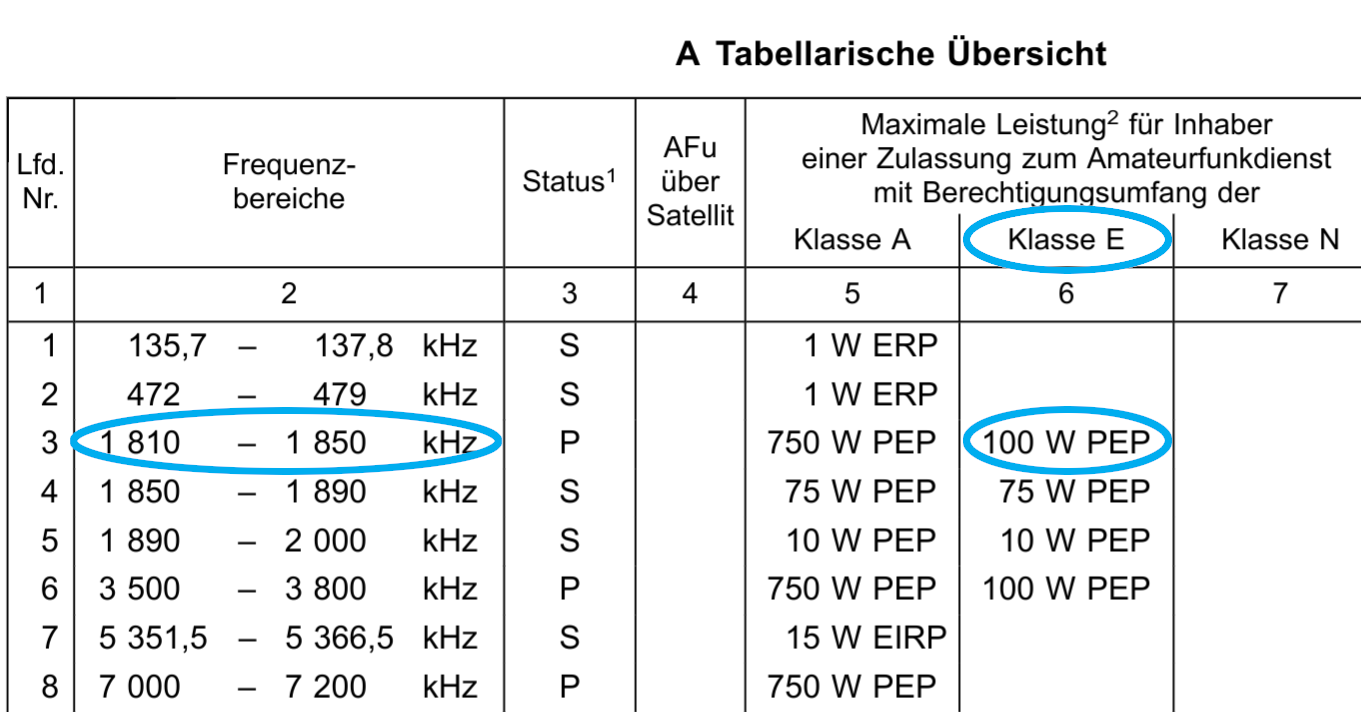
\includegraphics[width=0.85\textwidth]{foto/145}
    \caption{\scriptsize Ausschnitt aus der Anlage 1 der Amateurfunkverordnung}
    \label{ausgangsleistung}
\end{figure}
\end{frame}

\begin{frame}Aktuell ist die Anlage 1 der AFuV (\textcolor{DARCblue}{\faLink~\href{https://50ohm.de/a1}{50ohm.de/a1}}) hier zu finden.

\end{frame}

\begin{frame}
\only<1>{
\begin{QQuestion}{VD727}{Was gilt für die Rufzeicheninhaber der Klasse~E im Frequenzbereich \qtyrange{1810}{1850}{\kHz}?}{Maximal \qty{750}{\W}~PEP}
{Maximal \qty{75}{\W}~PEP }
{Maximal \qty{100}{\W}~PEP}
{Maximal \qty{10}{\W}~PEP}
\end{QQuestion}

}
\only<2>{
\begin{QQuestion}{VD727}{Was gilt für die Rufzeicheninhaber der Klasse~E im Frequenzbereich \qtyrange{1810}{1850}{\kHz}?}{Maximal \qty{750}{\W}~PEP}
{Maximal \qty{75}{\W}~PEP }
{\textbf{\textcolor{DARCgreen}{Maximal \qty{100}{\W}~PEP}}}
{Maximal \qty{10}{\W}~PEP}
\end{QQuestion}

}
\end{frame}

\begin{frame}
\only<1>{
\begin{QQuestion}{VD729}{Was gilt für die Rufzeicheninhaber der Klassen~A~und~E im Frequenzbereich \qtyrange{3,5}{3,8}{\MHz}?}{Maximal \qty{150}{\W}~PEP für Klasse~A und maximal \qty{10}{\W}~PEP für Klasse~E}
{Maximal \qty{10}{\W}~PEP für beide Klassen}
{Maximal \qty{750}{\W}~PEP für beide Klassen}
{Maximal \qty{750}{\W}~PEP für Klasse~A und maximal \qty{100}{\W}~PEP für Klasse~E}
\end{QQuestion}

}
\only<2>{
\begin{QQuestion}{VD729}{Was gilt für die Rufzeicheninhaber der Klassen~A~und~E im Frequenzbereich \qtyrange{3,5}{3,8}{\MHz}?}{Maximal \qty{150}{\W}~PEP für Klasse~A und maximal \qty{10}{\W}~PEP für Klasse~E}
{Maximal \qty{10}{\W}~PEP für beide Klassen}
{Maximal \qty{750}{\W}~PEP für beide Klassen}
{\textbf{\textcolor{DARCgreen}{Maximal \qty{750}{\W}~PEP für Klasse~A und maximal \qty{100}{\W}~PEP für Klasse~E}}}
\end{QQuestion}

}
\end{frame}

\begin{frame}
\only<1>{
\begin{QQuestion}{VD728}{Wie hoch ist die maximal zulässige Senderausgangsleistung für Rufzeicheninhaber der Klasse~A im Frequenzbereich \qtyrange{3,5}{3,8}{\MHz}?}{\qty{75}{\W}~PEP}
{\qty{750}{\W}~PEP}
{\qty{150}{\W}~PEP}
{\qty{100}{\W}~PEP}
\end{QQuestion}

}
\only<2>{
\begin{QQuestion}{VD728}{Wie hoch ist die maximal zulässige Senderausgangsleistung für Rufzeicheninhaber der Klasse~A im Frequenzbereich \qtyrange{3,5}{3,8}{\MHz}?}{\qty{75}{\W}~PEP}
{\textbf{\textcolor{DARCgreen}{\qty{750}{\W}~PEP}}}
{\qty{150}{\W}~PEP}
{\qty{100}{\W}~PEP}
\end{QQuestion}

}
\end{frame}

\begin{frame}
\only<1>{
\begin{QQuestion}{VD730}{Wie hoch ist die maximal zulässige Senderausgangsleistung für Rufzeicheninhaber der Klasse~A im Frequenzbereich \qtyrange{10,1}{10,15}{\MHz}?}{\qty{75}{\W}~PEP}
{\qty{150}{\W}~PEP}
{\qty{250}{\W}~PEP}
{\qty{750}{\W}~PEP}
\end{QQuestion}

}
\only<2>{
\begin{QQuestion}{VD730}{Wie hoch ist die maximal zulässige Senderausgangsleistung für Rufzeicheninhaber der Klasse~A im Frequenzbereich \qtyrange{10,1}{10,15}{\MHz}?}{\qty{75}{\W}~PEP}
{\textbf{\textcolor{DARCgreen}{\qty{150}{\W}~PEP}}}
{\qty{250}{\W}~PEP}
{\qty{750}{\W}~PEP}
\end{QQuestion}

}
\end{frame}

\begin{frame}
\only<1>{
\begin{QQuestion}{VD731}{Wie hoch ist die maximal zulässige Senderausgangsleistung für Rufzeicheninhaber der Klasse~A in den Frequenzbereichen \qtyrange{14,000}{14,350}{\MHz} und \qtyrange{18,068}{18,168}{\MHz}?}{\qty{150}{\W}~PEP}
{\qty{75}{\W}~PEP}
{\qty{750}{\W}~PEP}
{\qty{250}{\W}~PEP}
\end{QQuestion}

}
\only<2>{
\begin{QQuestion}{VD731}{Wie hoch ist die maximal zulässige Senderausgangsleistung für Rufzeicheninhaber der Klasse~A in den Frequenzbereichen \qtyrange{14,000}{14,350}{\MHz} und \qtyrange{18,068}{18,168}{\MHz}?}{\qty{150}{\W}~PEP}
{\qty{75}{\W}~PEP}
{\textbf{\textcolor{DARCgreen}{\qty{750}{\W}~PEP}}}
{\qty{250}{\W}~PEP}
\end{QQuestion}

}
\end{frame}

\begin{frame}
\only<1>{
\begin{QQuestion}{VD732}{Wie hoch ist die maximal zulässige Senderausgangsleistung für Rufzeicheninhaber der Klasse~A in den Frequenzbereichen \qtyrange{21,000}{21,450}{\MHz} und \qtyrange{24,890}{24,990}{\MHz}?}{\qty{150}{\W}~PEP}
{\qty{75}{\W}~PEP}
{\qty{750}{\W}~PEP}
{\qty{250}{\W}~PEP}
\end{QQuestion}

}
\only<2>{
\begin{QQuestion}{VD732}{Wie hoch ist die maximal zulässige Senderausgangsleistung für Rufzeicheninhaber der Klasse~A in den Frequenzbereichen \qtyrange{21,000}{21,450}{\MHz} und \qtyrange{24,890}{24,990}{\MHz}?}{\qty{150}{\W}~PEP}
{\qty{75}{\W}~PEP}
{\textbf{\textcolor{DARCgreen}{\qty{750}{\W}~PEP}}}
{\qty{250}{\W}~PEP}
\end{QQuestion}

}
\end{frame}

\begin{frame}
\only<1>{
\begin{QQuestion}{VD733}{Welche Leistungsgrenzen gelten für die Rufzeicheninhaber der Klassen~A~und~E in den Frequenzbereichen \qtyrange{21,000}{21,450}{\MHz} und \qtyrange{28,000}{29,700}{\MHz}?}{Maximal \qty{100}{\W}~PEP für Klasse~A und maximal \qty{10}{\W}~PEP für Klasse~E}
{Maximal \qty{200}{\W}~PEP für beide Klassen}
{Maximal \qty{750}{\W}~PEP für Klasse~A und maximal \qty{100}{\W}~PEP für Klasse~E}
{Maximal \qty{100}{\W}~PEP für beide Klassen}
\end{QQuestion}

}
\only<2>{
\begin{QQuestion}{VD733}{Welche Leistungsgrenzen gelten für die Rufzeicheninhaber der Klassen~A~und~E in den Frequenzbereichen \qtyrange{21,000}{21,450}{\MHz} und \qtyrange{28,000}{29,700}{\MHz}?}{Maximal \qty{100}{\W}~PEP für Klasse~A und maximal \qty{10}{\W}~PEP für Klasse~E}
{Maximal \qty{200}{\W}~PEP für beide Klassen}
{\textbf{\textcolor{DARCgreen}{Maximal \qty{750}{\W}~PEP für Klasse~A und maximal \qty{100}{\W}~PEP für Klasse~E}}}
{Maximal \qty{100}{\W}~PEP für beide Klassen}
\end{QQuestion}

}
\end{frame}

\begin{frame}
\only<1>{
\begin{QQuestion}{VD734}{Welche Leistungsgrenzen gelten für die Rufzeicheninhaber der Klasse~A~und~E in den Frequenzbereichen \qtyrange{144}{146}{\MHz} und \qtyrange{430}{440}{\MHz}?}{Maximal \qty{750}{\W}~PEP für beide Klassen}
{Maximal \qty{750}{\W}~PEP für Klasse~A und \qty{75}{\W}~PEP für Klasse~E}
{Maximal \qty{100}{\W}~PEP für Klasse~A und \qty{50}{\W}~PEP für Klasse~E}
{Maximal \qty{10}{\W}~PEP für beide Klassen}
\end{QQuestion}

}
\only<2>{
\begin{QQuestion}{VD734}{Welche Leistungsgrenzen gelten für die Rufzeicheninhaber der Klasse~A~und~E in den Frequenzbereichen \qtyrange{144}{146}{\MHz} und \qtyrange{430}{440}{\MHz}?}{Maximal \qty{750}{\W}~PEP für beide Klassen}
{\textbf{\textcolor{DARCgreen}{Maximal \qty{750}{\W}~PEP für Klasse~A und \qty{75}{\W}~PEP für Klasse~E}}}
{Maximal \qty{100}{\W}~PEP für Klasse~A und \qty{50}{\W}~PEP für Klasse~E}
{Maximal \qty{10}{\W}~PEP für beide Klassen}
\end{QQuestion}

}
\end{frame}

\begin{frame}
\only<1>{
\begin{QQuestion}{VD736}{Wie hoch ist die maximal zulässige Senderausgangsleistung für Rufzeicheninhaber der Klasse~A in den Amateurfunkbändern zwischen \qty{1300}{\MHz} und \qty{250}{\GHz}?}{\qty{750}{\W}~PEP}
{\qty{100}{\W}~PEP}
{\qty{150}{\W}~PEP}
{\qty{75}{\W}~PEP}
\end{QQuestion}

}
\only<2>{
\begin{QQuestion}{VD736}{Wie hoch ist die maximal zulässige Senderausgangsleistung für Rufzeicheninhaber der Klasse~A in den Amateurfunkbändern zwischen \qty{1300}{\MHz} und \qty{250}{\GHz}?}{\qty{750}{\W}~PEP}
{\qty{100}{\W}~PEP}
{\qty{150}{\W}~PEP}
{\textbf{\textcolor{DARCgreen}{\qty{75}{\W}~PEP}}}
\end{QQuestion}

}
\end{frame}

\begin{frame}
\only<1>{
\begin{QQuestion}{VD737}{Wie hoch ist die maximal zulässige Senderausgangsleistung für Rufzeicheninhaber der
Klasse E in den Amateurfunkbändern zwischen \qty{1300}{\MHz} und \qty{250}{\GHz}?}{Maximal \qty{75}{\W}~PEP}
{Maximal \qty{5}{\W}~PEP }
{Maximal \qty{100}{\W}~PEP}
{Maximal \qty{1}{\W}~PEP}
\end{QQuestion}

}
\only<2>{
\begin{QQuestion}{VD737}{Wie hoch ist die maximal zulässige Senderausgangsleistung für Rufzeicheninhaber der
Klasse E in den Amateurfunkbändern zwischen \qty{1300}{\MHz} und \qty{250}{\GHz}?}{Maximal \qty{75}{\W}~PEP}
{\textbf{\textcolor{DARCgreen}{Maximal \qty{5}{\W}~PEP }}}
{Maximal \qty{100}{\W}~PEP}
{Maximal \qty{1}{\W}~PEP}
\end{QQuestion}

}
\end{frame}

\begin{frame}\begin{itemize}
  \item Für den Frequenzbereich von \qtyrange{1240}{1300}{\mega\hertz} gelten zusätzliche Regelungen
  \item stehen nicht direkt in der Tabelle
  \item In der rechten Spalte \enquote{Zusätzliche Nutzungsbestimmungen gemäß B} kennzeichnen Zahlen ergänzende Angaben
  \item Stehen unter der Tabelle
  \item Für die folgende Frage ist der Punkt 11 zu beachten
  \end{itemize}
\end{frame}

\begin{frame}
\only<1>{
\begin{QQuestion}{VD735}{Wie hoch ist die maximal zulässige Sendeleistung für Rufzeicheninhaber der Klasse~A im Frequenzbereich \qtyrange{1240}{1300}{\MHz}?}{\qty{250}{\W}~PEP}
{\qty{100}{\W}~PEP}
{\qty{750}{\W}~PEP, jedoch nur maximal \qty{5}{\W}~EIRP im Teilbereich \qtyrange{1247}{1263}{\MHz}}
{\qty{75}{\W}~PEP, jedoch nur maximal \qty{5}{\W}~EIRP im Teilbereich \qtyrange{1247}{1263}{\MHz}}
\end{QQuestion}

}
\only<2>{
\begin{QQuestion}{VD735}{Wie hoch ist die maximal zulässige Sendeleistung für Rufzeicheninhaber der Klasse~A im Frequenzbereich \qtyrange{1240}{1300}{\MHz}?}{\qty{250}{\W}~PEP}
{\qty{100}{\W}~PEP}
{\textbf{\textcolor{DARCgreen}{\qty{750}{\W}~PEP, jedoch nur maximal \qty{5}{\W}~EIRP im Teilbereich \qtyrange{1247}{1263}{\MHz}}}}
{\qty{75}{\W}~PEP, jedoch nur maximal \qty{5}{\W}~EIRP im Teilbereich \qtyrange{1247}{1263}{\MHz}}
\end{QQuestion}

}
\end{frame}%ENDCONTENT


\section{Senderausgangsleistung}
\label{section:senderausgangsleistung}
\begin{frame}%STARTCONTENT
\begin{itemize}
  \item Verpflichtung von Funkamateuren die Leistungsgrenzwerte ihrer Funkanlage einzuhalten
  \item Auf vielen Amateurfunkbändern gilt eine \emph{maximale Senderausgangsleistung} (\emph{PEP}, Peak-Envelope-Power) als Grenzwert
  \item Auch unerwünschte Aussendungen sind von Bedeutung
  \end{itemize}
\end{frame}

\begin{frame}
\frametitle{Messung von unerwünschten Aussendungen}
\begin{itemize}
  \item Am Senderausgang
  \item Unter Einzebiehung von Stehwellenmessgerät, Anpassgerät(e), Tiefpassfilter etc.
  \item Messsung von unerwünschen Aussendungen, die die Antenne erreichen können
  \end{itemize}
\end{frame}

\begin{frame}
\only<1>{
\begin{QQuestion}{EJ209}{Wie erfolgt die Messung der Leistungen, die zu unerwünschten Aussendungen führen?}{Die Messung erfolgt am Senderausgang mit einem hochohmigen HF-Tastkopf und angeschlossenem Transistorvoltmeter.}
{Die Messung erfolgt am Fußpunkt der im Funkbetrieb verwendeten Antenne unter Einbeziehung des gegebenenfalls verwendeten Antennenanpassgeräts.}
{Die Messung erfolgt am Ausgang der Antennenleitung unter Einbeziehung des im Funkbetrieb verwendeten Antennenanpassgeräts.}
{Die Messung erfolgt am Senderausgang unter Einbeziehung des gegebenenfalls verwendeten Stehwellenmessgeräts und des gegebenenfalls verwendeten Tiefpassfilters.}
\end{QQuestion}

}
\only<2>{
\begin{QQuestion}{EJ209}{Wie erfolgt die Messung der Leistungen, die zu unerwünschten Aussendungen führen?}{Die Messung erfolgt am Senderausgang mit einem hochohmigen HF-Tastkopf und angeschlossenem Transistorvoltmeter.}
{Die Messung erfolgt am Fußpunkt der im Funkbetrieb verwendeten Antenne unter Einbeziehung des gegebenenfalls verwendeten Antennenanpassgeräts.}
{Die Messung erfolgt am Ausgang der Antennenleitung unter Einbeziehung des im Funkbetrieb verwendeten Antennenanpassgeräts.}
{\textbf{\textcolor{DARCgreen}{Die Messung erfolgt am Senderausgang unter Einbeziehung des gegebenenfalls verwendeten Stehwellenmessgeräts und des gegebenenfalls verwendeten Tiefpassfilters.}}}
\end{QQuestion}

}
\end{frame}

\begin{frame}
\frametitle{Messung der Senderausgangsleistung}
\begin{itemize}
  \item Direkt am Senderausgang
  \item Ohne Zusatzgeräte, Filter oder Kabel
  \item Bei SSB $\rightarrow$ mit Modulation
  \item Ein- oder Zweitonaussteuerung, aber keine Sprache
  \item Messung der maximalen \emph{Hüllkurvenleistung} (PEP)
  \item Spitzenleistung des Senders bei maximaler Aussteuerung
  \end{itemize}

\end{frame}

\begin{frame}
\only<1>{
\begin{QQuestion}{EF401}{Die Ausgangsleistung eines Senders ist die unmittelbar nach~...}{dem Senderausgang gemessene Summe aus vorlaufender und rücklaufender Leistung.}
{dem Senderausgang gemessene Differenz aus vorlaufender und rücklaufender Leistung.}
{der Antenne messbaren Leistung, die durch ein Feldstärkenmessgerät im Nahfeld ermittelt werden kann.}
{dem Senderausgang messbare Leistung, bevor sie Zusatzgeräte durchläuft.}
\end{QQuestion}

}
\only<2>{
\begin{QQuestion}{EF401}{Die Ausgangsleistung eines Senders ist die unmittelbar nach~...}{dem Senderausgang gemessene Summe aus vorlaufender und rücklaufender Leistung.}
{dem Senderausgang gemessene Differenz aus vorlaufender und rücklaufender Leistung.}
{der Antenne messbaren Leistung, die durch ein Feldstärkenmessgerät im Nahfeld ermittelt werden kann.}
{\textbf{\textcolor{DARCgreen}{dem Senderausgang messbare Leistung, bevor sie Zusatzgeräte durchläuft.}}}
\end{QQuestion}

}
\end{frame}

\begin{frame}
\only<1>{
\begin{QQuestion}{EF402}{Wie und wo wird die Ausgangsleistung eines SSB-Senders gemessen? Die maximale Hüllkurvenleistung (PEP) wird gemessen...}{zwischen Antennentuner und Speisepunkt bei Sprachmodulation.}
{zwischen Antennentuner und Speisepunkt der Antenne mit unmoduliertem Träger.}
{direkt am Senderausgang bei Ein- oder Zweitonaussteuerung.}
{direkt am Senderausgang mit unmoduliertem Träger.}
\end{QQuestion}

}
\only<2>{
\begin{QQuestion}{EF402}{Wie und wo wird die Ausgangsleistung eines SSB-Senders gemessen? Die maximale Hüllkurvenleistung (PEP) wird gemessen...}{zwischen Antennentuner und Speisepunkt bei Sprachmodulation.}
{zwischen Antennentuner und Speisepunkt der Antenne mit unmoduliertem Träger.}
{\textbf{\textcolor{DARCgreen}{direkt am Senderausgang bei Ein- oder Zweitonaussteuerung.}}}
{direkt am Senderausgang mit unmoduliertem Träger.}
\end{QQuestion}

}
\end{frame}%ENDCONTENT


\section{Messungen am Sender}
\label{section:sender_messungen}
\begin{frame}%STARTCONTENT

\only<1>{
\begin{PQuestion}{AI608}{Was stellt die folgende Schaltung dar? }{Absorptionsfrequenzmesser}
{Messkopf zur HF-Leistungsmessung}
{Antennenimpedanzmesser}
{HF-Dipmeter}
{\DARCimage{1.0\linewidth}{576include}}\end{PQuestion}

}
\only<2>{
\begin{PQuestion}{AI608}{Was stellt die folgende Schaltung dar? }{Absorptionsfrequenzmesser}
{\textbf{\textcolor{DARCgreen}{Messkopf zur HF-Leistungsmessung}}}
{Antennenimpedanzmesser}
{HF-Dipmeter}
{\DARCimage{1.0\linewidth}{576include}}\end{PQuestion}

}
\end{frame}

\begin{frame}
\only<1>{
\begin{PQuestion}{AI605}{Was stellt die folgende Schaltung dar? }{Absorptionsfrequenzmesser}
{HF-Tastkopf}
{Antennenimpedanzmesser}
{HF-Dipmeter}
{\DARCimage{1.0\linewidth}{770include}}\end{PQuestion}

}
\only<2>{
\begin{PQuestion}{AI605}{Was stellt die folgende Schaltung dar? }{Absorptionsfrequenzmesser}
{\textbf{\textcolor{DARCgreen}{HF-Tastkopf}}}
{Antennenimpedanzmesser}
{HF-Dipmeter}
{\DARCimage{1.0\linewidth}{770include}}\end{PQuestion}

}
\end{frame}

\begin{frame}
\only<1>{
\begin{PQuestion}{AI604}{Wozu dient diese Schaltung? Sie dient~...}{als Messkopf zum Abgleich von HF-Schaltungen.}
{als hochohmiger Messkopf für einen vektoriellen Netzwerkanalyzer.}
{zur Messung der Resonanzfrequenz mit einem Frequenzzähler.}
{als Gleichspannungstastkopf zur genauen Einstellung der Versorgungsspannung.}
{\DARCimage{1.0\linewidth}{770include}}\end{PQuestion}

}
\only<2>{
\begin{PQuestion}{AI604}{Wozu dient diese Schaltung? Sie dient~...}{\textbf{\textcolor{DARCgreen}{als Messkopf zum Abgleich von HF-Schaltungen.}}}
{als hochohmiger Messkopf für einen vektoriellen Netzwerkanalyzer.}
{zur Messung der Resonanzfrequenz mit einem Frequenzzähler.}
{als Gleichspannungstastkopf zur genauen Einstellung der Versorgungsspannung.}
{\DARCimage{1.0\linewidth}{770include}}\end{PQuestion}

}
\end{frame}

\begin{frame}
\only<1>{
\begin{PQuestion}{AI609}{Sie wollen mit der folgenden Messschaltung die Ausgangsleistung eines \qty{2}{\m}-Senders überprüfen, der voraussichtlich ca. \qty{15}{\W} HF-Leistung liefert. Was sollte für die Messung vor die dargestellte Messschaltung geschaltet werden?}{Dämpfungsglied \qty{20}{\decibel}, \qty{20}{\W}}
{\qty{25}{\m} langes Koaxialkabel vom Typ RG213 (MIL)}
{Stehwellenmessgerät}
{Adapter BNC-Buchse auf N-Stecker}
{\DARCimage{1.0\linewidth}{576include}}\end{PQuestion}

}
\only<2>{
\begin{PQuestion}{AI609}{Sie wollen mit der folgenden Messschaltung die Ausgangsleistung eines \qty{2}{\m}-Senders überprüfen, der voraussichtlich ca. \qty{15}{\W} HF-Leistung liefert. Was sollte für die Messung vor die dargestellte Messschaltung geschaltet werden?}{\textbf{\textcolor{DARCgreen}{Dämpfungsglied \qty{20}{\decibel}, \qty{20}{\W}}}}
{\qty{25}{\m} langes Koaxialkabel vom Typ RG213 (MIL)}
{Stehwellenmessgerät}
{Adapter BNC-Buchse auf N-Stecker}
{\DARCimage{1.0\linewidth}{576include}}\end{PQuestion}

}
\end{frame}

\begin{frame}
\only<1>{
\begin{PQuestion}{AI612}{Was muss für die genaue Messung der HF-Ausgangsleistung eines Senders mit einer solchen Schaltung berücksichtigt werden?}{Bei den Umrechnungen darf nur mit dem Effektivwert gerechnet werden.}
{$R_1$ muss genau \qty{50}{\ohm} betragen.}
{Korrekturwerte für die Schaltung, die aus einer Kalibrierung stammen.}
{Die Schaltung muss vor jeder Messung mit einem Spektrumanalysator überprüft werden.}
{\DARCimage{1.0\linewidth}{577include}}\end{PQuestion}

}
\only<2>{
\begin{PQuestion}{AI612}{Was muss für die genaue Messung der HF-Ausgangsleistung eines Senders mit einer solchen Schaltung berücksichtigt werden?}{Bei den Umrechnungen darf nur mit dem Effektivwert gerechnet werden.}
{$R_1$ muss genau \qty{50}{\ohm} betragen.}
{\textbf{\textcolor{DARCgreen}{Korrekturwerte für die Schaltung, die aus einer Kalibrierung stammen.}}}
{Die Schaltung muss vor jeder Messung mit einem Spektrumanalysator überprüft werden.}
{\DARCimage{1.0\linewidth}{577include}}\end{PQuestion}

}
\end{frame}

\begin{frame}
\only<1>{
\begin{PQuestion}{AI610}{Dem Eingang der folgenden Messschaltung wird eine HF-Leistung von \qty{1}{\W} zugeführt. D ist eine Schottkydiode mit $U_F$ = \qty{0,23}{\V}. Welche Spannung $U_A$ ist am Ausgang A zu erwarten, wenn die Messung mit einem hochohmigen Spannungsmessgerät erfolgt?}{\qty{9,8}{\V}}
{\qty{3,3}{\V}}
{\qty{7,1}{\V}}
{\qty{4,8}{\V}}
{\DARCimage{1.0\linewidth}{576include}}\end{PQuestion}

}
\only<2>{
\begin{PQuestion}{AI610}{Dem Eingang der folgenden Messschaltung wird eine HF-Leistung von \qty{1}{\W} zugeführt. D ist eine Schottkydiode mit $U_F$ = \qty{0,23}{\V}. Welche Spannung $U_A$ ist am Ausgang A zu erwarten, wenn die Messung mit einem hochohmigen Spannungsmessgerät erfolgt?}{\qty{9,8}{\V}}
{\qty{3,3}{\V}}
{\qty{7,1}{\V}}
{\textbf{\textcolor{DARCgreen}{\qty{4,8}{\V}}}}
{\DARCimage{1.0\linewidth}{576include}}\end{PQuestion}

}
\end{frame}

\begin{frame}
\frametitle{Lösungsweg}
\begin{itemize}
  \item gegeben: $P_E = 1W$
  \item gegeben: $U_F = 0,23V$
  \item gegeben: $R_V = 110Ω$, $R_T = 330Ω$
  \item gesucht: $U_A$
  \end{itemize}
    \pause
    $R = (\frac{1}{R_T + R_T} + \frac{1}{R_V} + \frac{1}{R_V})^{-1} = (\frac{1}{330Ω + 330Ω} + \frac{1}{110Ω} + \frac{1}{110Ω})^{-1} = 50,77Ω$
    \pause
    $P_E = \frac{U_{E,eff}^2}{R} \Rightarrow U_{E,eff} = \sqrt{P_E \cdot R} = \sqrt{1W \cdot 50,77Ω} = 7,125V$

$U_S = U_{E,eff} \cdot \sqrt{2} = 7,071V \cdot 1,414 = 10,07V$
    \pause
    $U_A = \frac{U_S}{2} -- U_F = \frac{10,07V}{2} -- 0,23V = 5,035V -- 0,23V = 4,805V \approx 4,8V$



\end{frame}

\begin{frame}
\only<1>{
\begin{PQuestion}{AI611}{Bei der folgenden Schaltung besteht $R_1$ aus einer Zusammenschaltung von Widerständen, die einen Gesamtwiderstand von \qty{54,1}{\ohm} hat und etwa \qty{200}{\W} aufnehmen kann. Die Diode ist eine Siliziumdiode mit $U_{\symup{F}}$ = \qty{0,7}{\V}. Am Ausgang wird mit einem digitalen Spannungsmessgerät eine Gleichspannung von \qty{14,9}{\V} gemessen. Wie groß ist etwa die HF-Leistung am Eingang der Schaltung?}{\qty{9,7}{\W}}
{\qty{37,8}{\W}}
{\qty{4,9}{\W}}
{\qty{19,4}{\W}}
{\DARCimage{1.0\linewidth}{577include}}\end{PQuestion}

}
\only<2>{
\begin{PQuestion}{AI611}{Bei der folgenden Schaltung besteht $R_1$ aus einer Zusammenschaltung von Widerständen, die einen Gesamtwiderstand von \qty{54,1}{\ohm} hat und etwa \qty{200}{\W} aufnehmen kann. Die Diode ist eine Siliziumdiode mit $U_{\symup{F}}$ = \qty{0,7}{\V}. Am Ausgang wird mit einem digitalen Spannungsmessgerät eine Gleichspannung von \qty{14,9}{\V} gemessen. Wie groß ist etwa die HF-Leistung am Eingang der Schaltung?}{\textbf{\textcolor{DARCgreen}{\qty{9,7}{\W}}}}
{\qty{37,8}{\W}}
{\qty{4,9}{\W}}
{\qty{19,4}{\W}}
{\DARCimage{1.0\linewidth}{577include}}\end{PQuestion}

}
\end{frame}

\begin{frame}
\frametitle{Lösungsweg}
\begin{itemize}
  \item gegeben: $U_A = 14,9V DC$
  \item gegeben: $U_F = 0,7V$
  \item gegeben: $R_1 = 54,1Ω$, $R_T = 330Ω$
  \item gesucht: $P_E$
  \end{itemize}
    \pause
    $R = (\frac{1}{R_T + R_T} + \frac{1}{R_1})^{-1} = (\frac{1}{330Ω + 330Ω} + \frac{1}{54,1Ω})^{-1} = 50Ω$
    \pause
    $U_S = (U_A + U_F) \cdot 2 = (14,9V + 0,7V) \cdot 2 = 31,2V$

$U_{E,eff} = \frac{U_S}{\sqrt{2}} = \frac{31,2V}{1,414} = 22,06V$
    \pause
    $P_E = \frac{U_{E,eff}^2}{R} = \frac{(22,06V)^2}{50Ω} \approx 9,7W$



\end{frame}

\begin{frame}
\only<1>{
\begin{PQuestion}{AI607}{Mit der folgenden Schaltung soll die Ausgangsleistung eines \qty{2}{\m}-FM-Handfunkgerätes gemessen werden. Die Dioden sind Schottkydioden mit $U_{\symup{F}}$~=~\qty{0,23}{\V}. Am Ausgang wird mit einem digitalen Spannungsmessgerät eine Gleichspannung von \qty{15,3}{\V} gemessen. Wie groß ist etwa die HF-Leistung am Eingang der Schaltung?}{Zirka \qty{1,2}{\W}}
{Zirka \qty{4,7}{\W}}
{Zirka \qty{600}{\mW}}
{Zirka \qty{2,4}{\W}}
{\DARCimage{1.0\linewidth}{771include}}\end{PQuestion}

}
\only<2>{
\begin{PQuestion}{AI607}{Mit der folgenden Schaltung soll die Ausgangsleistung eines \qty{2}{\m}-FM-Handfunkgerätes gemessen werden. Die Dioden sind Schottkydioden mit $U_{\symup{F}}$~=~\qty{0,23}{\V}. Am Ausgang wird mit einem digitalen Spannungsmessgerät eine Gleichspannung von \qty{15,3}{\V} gemessen. Wie groß ist etwa die HF-Leistung am Eingang der Schaltung?}{Zirka \qty{1,2}{\W}}
{Zirka \qty{4,7}{\W}}
{\textbf{\textcolor{DARCgreen}{Zirka \qty{600}{\mW}}}}
{Zirka \qty{2,4}{\W}}
{\DARCimage{1.0\linewidth}{771include}}\end{PQuestion}

}
\end{frame}

\begin{frame}
\frametitle{Lösungsweg}
\begin{itemize}
  \item gegeben: $U_A = 15,3V DC$
  \item gegeben: $U_F = 0,23V$
  \item gegeben: $R_{V1} = 56Ω$, $R_{V2} = 470Ω$
  \item gesucht: $P_E$
  \end{itemize}
    \pause
    $R = (\frac{1}{R_{V1}} + \frac{1}{R_{V2}})^{-1} = (\frac{1}{R_{56Ω}} + \frac{1}{R_{470Ω}})^{-1} = 50,04Ω$
    \pause
    $U_S = \frac{U_A}{2} + U_F = \frac{15,3V}{2} + 0,23V = 7,88V$

$U_{E,eff} = \frac{U_S}{\sqrt{2}} = \frac{7,88V}{1,414} = 5,57V$
    \pause
    $P_E = \frac{U_{E,eff}^2}{R} = \frac{{5,57V}^2}{50,04Ω} \approx 600mW$



\end{frame}

\begin{frame}
\only<1>{
\begin{PQuestion}{AI606}{Die Leistung eines \qty{2}{\metre}-Senders soll mit einer künstlichen \qty{50}{\ohm}-Antenne bestimmt werden, die über eine Anzapfung bei \qty{5}{\ohm} vom erdnahen Ende verfügt. Zur Messung an diesem Punkt wird die folgende Schaltung eingesetzt. Die Dioden sind Schottkydioden mit $U_{\symup{F}}~=$~\qty{0,23}{\V}. Am Ausgang der Schaltung wird dabei mit einem digitalen Spannungsmessgerät eine Gleichspannung von \qty{15,3}{\V} gemessen. Wie groß ist etwa die HF-Leistung des Senders?}{Zirka \qty{60}{\W}}
{Zirka \qty{480}{\W}}
{Zirka \qty{340}{\W}}
{Zirka \qty{240}{\W}}
{\DARCimage{1.0\linewidth}{770include}}\end{PQuestion}

}
\only<2>{
\begin{PQuestion}{AI606}{Die Leistung eines \qty{2}{\metre}-Senders soll mit einer künstlichen \qty{50}{\ohm}-Antenne bestimmt werden, die über eine Anzapfung bei \qty{5}{\ohm} vom erdnahen Ende verfügt. Zur Messung an diesem Punkt wird die folgende Schaltung eingesetzt. Die Dioden sind Schottkydioden mit $U_{\symup{F}}~=$~\qty{0,23}{\V}. Am Ausgang der Schaltung wird dabei mit einem digitalen Spannungsmessgerät eine Gleichspannung von \qty{15,3}{\V} gemessen. Wie groß ist etwa die HF-Leistung des Senders?}{\textbf{\textcolor{DARCgreen}{Zirka \qty{60}{\W}}}}
{Zirka \qty{480}{\W}}
{Zirka \qty{340}{\W}}
{Zirka \qty{240}{\W}}
{\DARCimage{1.0\linewidth}{770include}}\end{PQuestion}

}
\end{frame}

\begin{frame}
\frametitle{Lösungsweg}
\begin{itemize}
  \item gegeben: $U_A = 15,3V DC$
  \item gegeben: $U_F = 0,23V$
  \item gegeben: $R = 50Ω$ aus dem Messsystem
  \item gegeben: $R_A = 5Ω$ (10:1 Spannungsteiler)
  \item gesucht: $P_E$
  \end{itemize}
    \pause
    $U_S = \frac{U_A}{2} + U_F = \frac{15,3V}{2} + 0,23V = 7,88V$

$U_{E,eff} = \frac{U_S}{\sqrt{2}} = \frac{7,88V}{1,414} = 5,57V$
    \pause
    $P_E = \frac{(U_{E,eff} \cdot 10)^2}{R} = \frac{(5,57V \cdot 10)^2}{50Ω} \approx 60W$



\end{frame}

\begin{frame}
\only<1>{
\begin{PQuestion}{AI613}{Was stellt die folgende Schaltung dar? }{Antennenimpedanzmesser}
{Einfacher Peilsender}
{Feldstärkeanzeiger}
{Resonanzmessgerät}
{\DARCimage{1.0\linewidth}{496include}}\end{PQuestion}

}
\only<2>{
\begin{PQuestion}{AI613}{Was stellt die folgende Schaltung dar? }{Antennenimpedanzmesser}
{Einfacher Peilsender}
{\textbf{\textcolor{DARCgreen}{Feldstärkeanzeiger}}}
{Resonanzmessgerät}
{\DARCimage{1.0\linewidth}{496include}}\end{PQuestion}

}
\end{frame}%ENDCONTENT


\section{Dummy-Load}
\label{section:dummy_load_1}
\begin{frame}%STARTCONTENT

\begin{columns}
    \begin{column}{0.48\textwidth}
    \begin{itemize}
  \item \emph{Dummy Load} wird für Abgleicharbeiten und Messungen an Sendern verwendet
  \item Ist ein Lastwiderstand
  \item Sendeleistung wird fast vollständig in Wärme umgesetzt
  \item auch: \emph{Abschlusswiderstand} oder \emph{künstliche Antenne}
  \end{itemize}

    \end{column}
   \begin{column}{0.48\textwidth}
       
\begin{figure}
    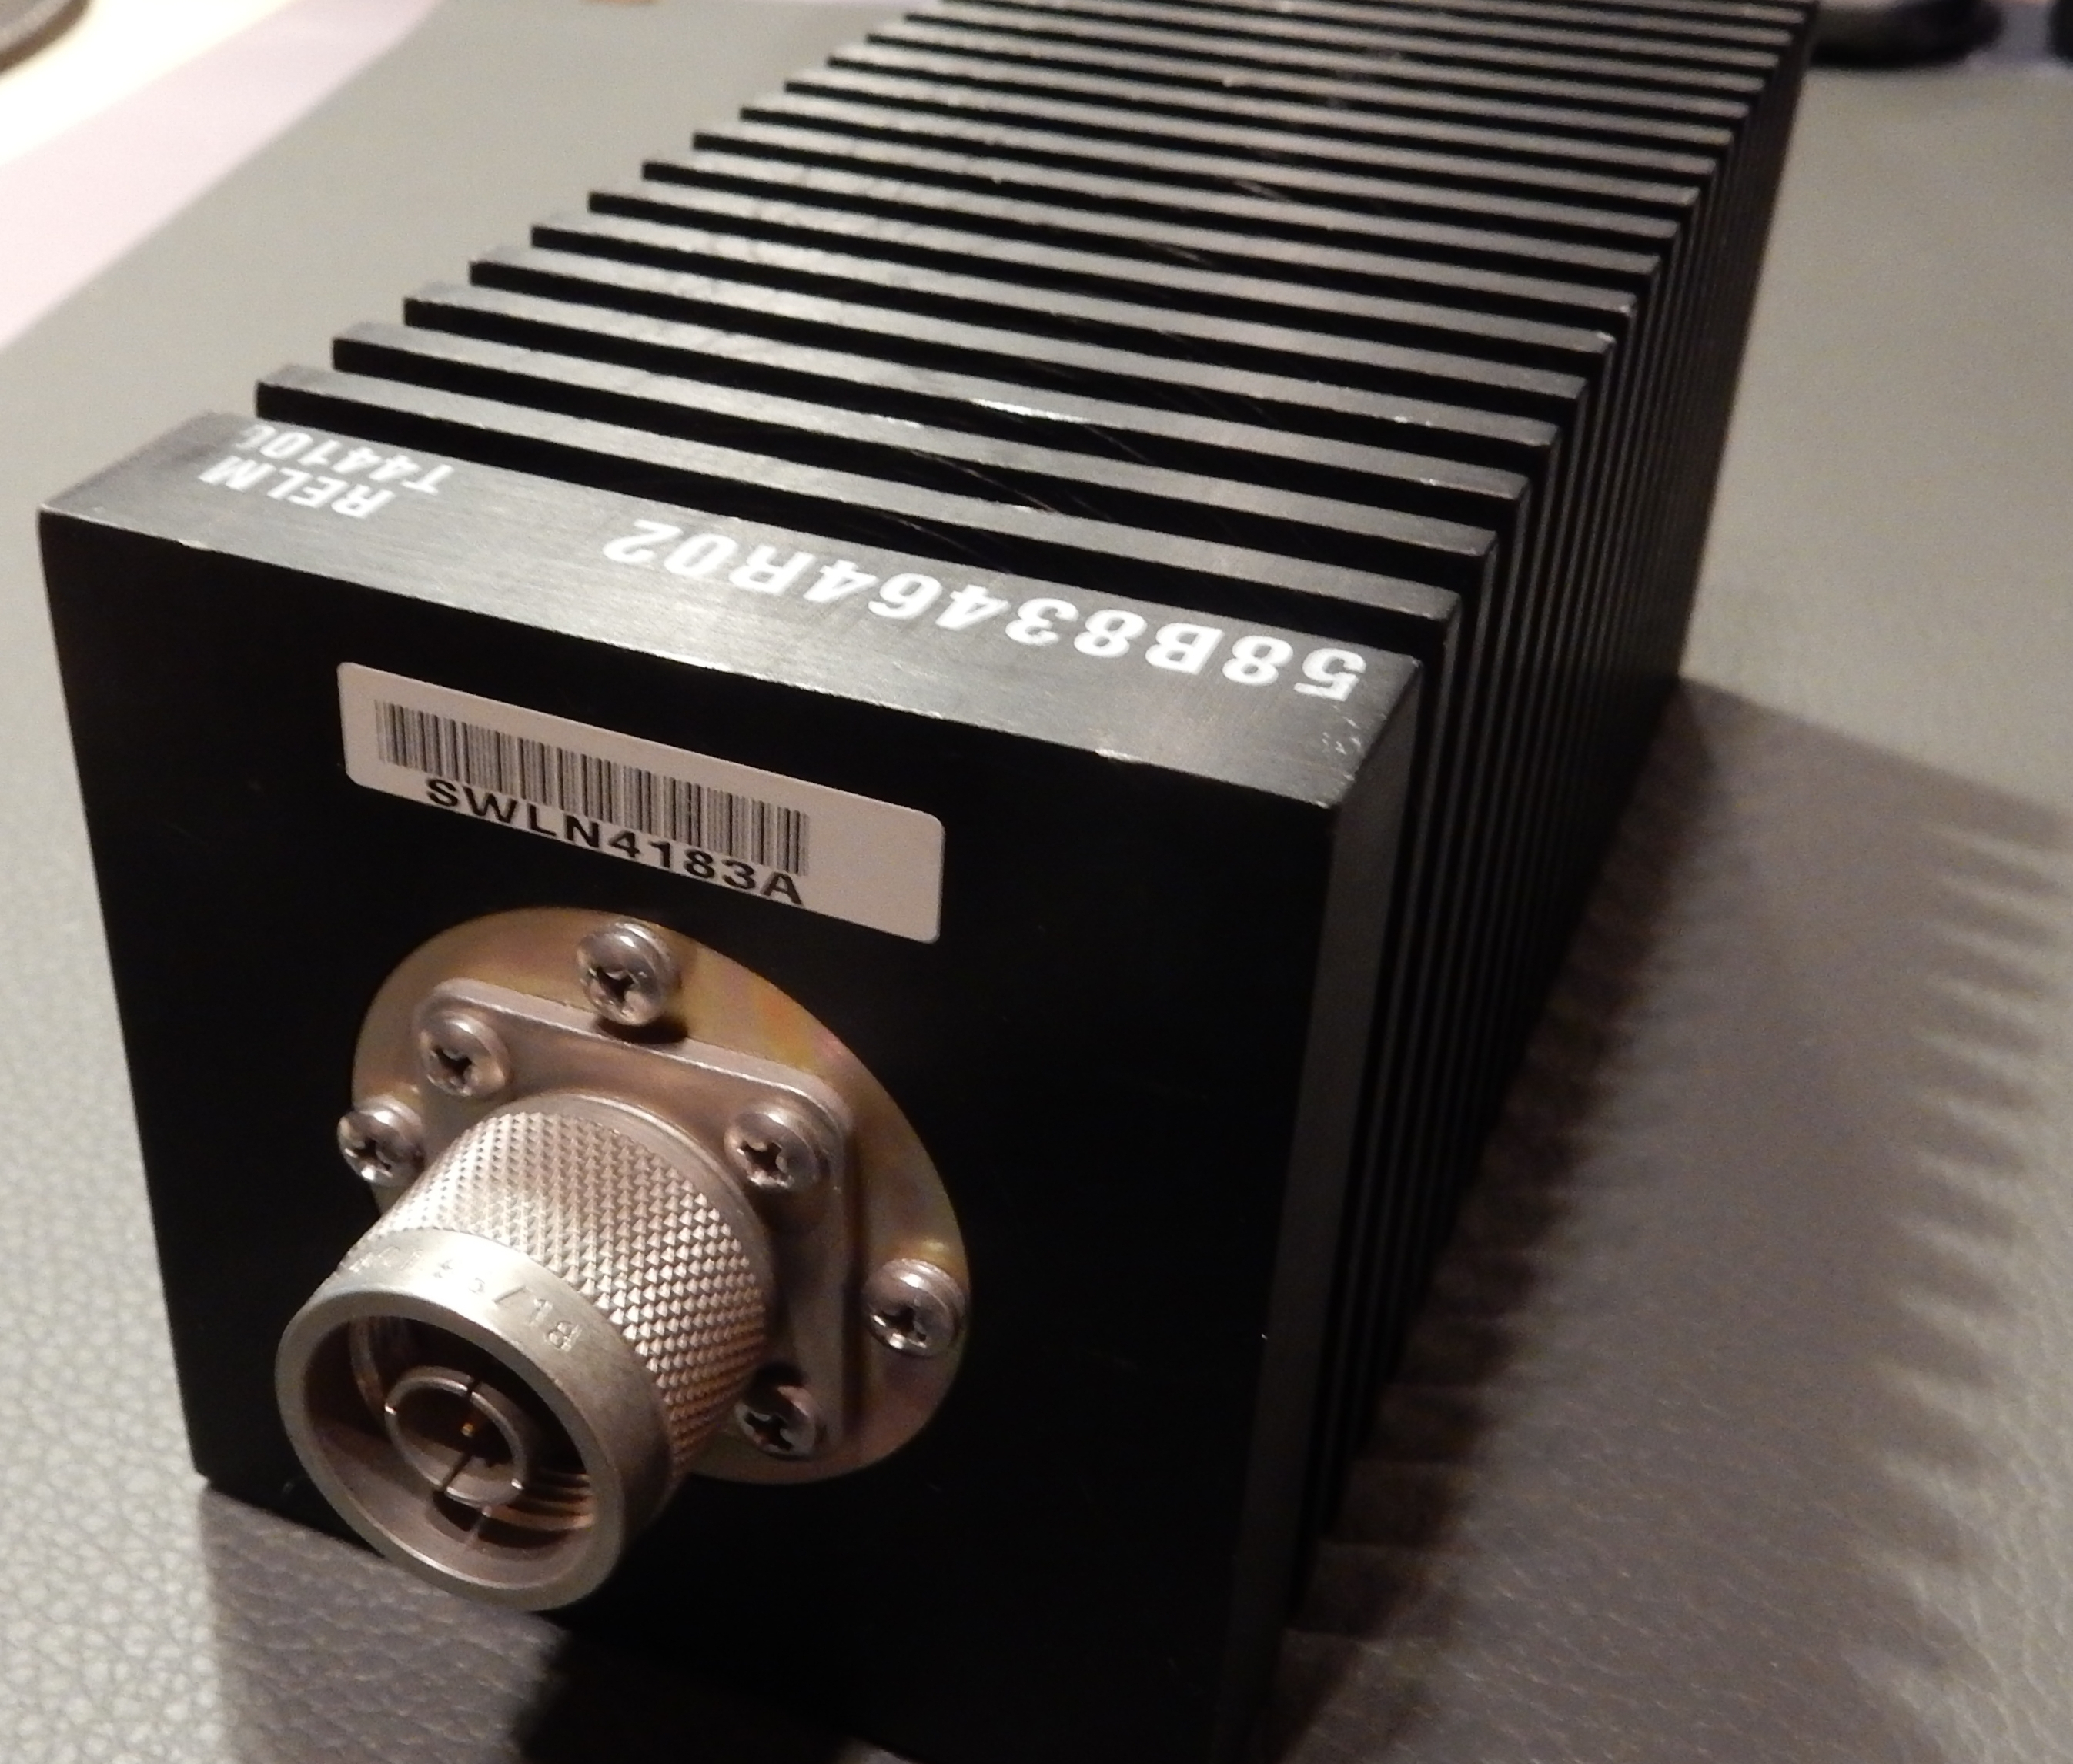
\includegraphics[width=0.85\textwidth]{foto/68}
    \caption{\scriptsize Dummy Load}
    \label{n_antennenanpassung_dummy_load}
\end{figure}

   \end{column}
\end{columns}

\end{frame}

\begin{frame}
\frametitle{Abgleicharbeiten und Messungen}
\begin{itemize}
  \item Immer an möglichst angepasster Antenne oder Dummy Load
  \item Ansonsten kann die Reflektion der Leistung die Endstufe zerstören
  \end{itemize}
\end{frame}

\begin{frame}
\only<1>{
\begin{QQuestion}{VD111}{Was ist bei Abgleicharbeiten und Messungen an Sendern im Hinblick auf die Aussendung zu beachten?}{Das Antennenkabel muss fest angeschlossen sein.}
{Das Sendergehäuse darf nicht geöffnet werden.}
{Es sind geeignete Maßnahmen zu treffen, die ein freies Abstrahlen von Signalen wirkungsvoll verhindern.}
{Es darf nur mit halber Sendeleistung gesendet werden.}
\end{QQuestion}

}
\only<2>{
\begin{QQuestion}{VD111}{Was ist bei Abgleicharbeiten und Messungen an Sendern im Hinblick auf die Aussendung zu beachten?}{Das Antennenkabel muss fest angeschlossen sein.}
{Das Sendergehäuse darf nicht geöffnet werden.}
{\textbf{\textcolor{DARCgreen}{Es sind geeignete Maßnahmen zu treffen, die ein freies Abstrahlen von Signalen wirkungsvoll verhindern.}}}
{Es darf nur mit halber Sendeleistung gesendet werden.}
\end{QQuestion}

}
\end{frame}

\begin{frame}
\only<1>{
\begin{QQuestion}{NJ202}{Wie verhindern Sie beim Abgleichen Ihres selbstgebauten Senders Störungen anderer Funkverbindungen?}{Ich sende nur mit halber Sendeleistung.}
{Ich führe die Abstimmarbeiten auf einer sogenannten ISM-Frequenz aus.}
{Ich verwende einen geeigneten Abschlusswiderstand (Dummy Load).}
{Ich versuche unnötige Modulation zu vermeiden.}
\end{QQuestion}

}
\only<2>{
\begin{QQuestion}{NJ202}{Wie verhindern Sie beim Abgleichen Ihres selbstgebauten Senders Störungen anderer Funkverbindungen?}{Ich sende nur mit halber Sendeleistung.}
{Ich führe die Abstimmarbeiten auf einer sogenannten ISM-Frequenz aus.}
{\textbf{\textcolor{DARCgreen}{Ich verwende einen geeigneten Abschlusswiderstand (Dummy Load).}}}
{Ich versuche unnötige Modulation zu vermeiden.}
\end{QQuestion}

}
\end{frame}

\begin{frame}
\only<1>{
\begin{QQuestion}{NF107}{Warum sollte ein Sender nie ohne angepasste Antenne oder Dummy Load betrieben werden?}{Durch die reflektierte Welle könnte die Senderendstufe beschädigt werden.}
{Durch die fehlende Last wird die Versorgungsspannung hochgeregelt, was zu Überspannungen führen kann. }
{Durch die absorbierte Leistung kann das Netzteil des Senders überlastet werden.  }
{Das Stehwellenmessgerät könnte beschädigt werden.}
\end{QQuestion}

}
\only<2>{
\begin{QQuestion}{NF107}{Warum sollte ein Sender nie ohne angepasste Antenne oder Dummy Load betrieben werden?}{\textbf{\textcolor{DARCgreen}{Durch die reflektierte Welle könnte die Senderendstufe beschädigt werden.}}}
{Durch die fehlende Last wird die Versorgungsspannung hochgeregelt, was zu Überspannungen führen kann. }
{Durch die absorbierte Leistung kann das Netzteil des Senders überlastet werden.  }
{Das Stehwellenmessgerät könnte beschädigt werden.}
\end{QQuestion}

}
\end{frame}

\begin{frame}
\frametitle{Abstimmen}
\begin{itemize}
  \item Aussendungen zum Abstimmen lassen sich nicht vermeiden
  \item Z.B. bei automatischen Anpassgeräten
  \item So kurz wie möglich
  \item Auf freier Frequenz
  \end{itemize}
\end{frame}

\begin{frame}
\only<1>{
\begin{QQuestion}{VD112}{Unter welcher Bedingung ist das Aussenden eines unmodulierten oder ungetasteten Trägers zulässig?}{Sofern es sich um ein digitales Signal handelt}
{Wenn es kurzzeitig erfolgt, z.~B. zum Abstimmen}
{Wenn die Übertragungsbedingungen keine weitreichenden Verbindungen zulassen}
{Sofern die Sendeleistung auf unter \qty{1}{\W} reduziert wird}
\end{QQuestion}

}
\only<2>{
\begin{QQuestion}{VD112}{Unter welcher Bedingung ist das Aussenden eines unmodulierten oder ungetasteten Trägers zulässig?}{Sofern es sich um ein digitales Signal handelt}
{\textbf{\textcolor{DARCgreen}{Wenn es kurzzeitig erfolgt, z.~B. zum Abstimmen}}}
{Wenn die Übertragungsbedingungen keine weitreichenden Verbindungen zulassen}
{Sofern die Sendeleistung auf unter \qty{1}{\W} reduziert wird}
\end{QQuestion}

}
\end{frame}%ENDCONTENT


\section{Dummy-Load II}
\label{section:dummy_load_2}
\begin{frame}%STARTCONTENT

\only<1>{
\begin{PQuestion}{AI601}{Die Darstellung zeigt eine aus \qty{150}{\ohm} / \qty{1}{\W}-Widerständen aufgebaute künstliche Antenne (Dummy Load). Mit dieser Kombination aus Reihen- und Parallelschaltung werden ca. \qty{50}{\ohm} erreicht. Wie viele Widerstände werden für diesen Aufbau benötigt und welche Dauerleistung verträgt diese künstliche Antenne?}{16~Widerstände, \qty{16}{\W}}
{48~Widerstände, \qty{12}{\W}}
{12~Widerstände, \qty{48}{\W}}
{48~Widerstände, \qty{48}{\W}}
{\DARCimage{1.0\linewidth}{47include}}\end{PQuestion}

}
\only<2>{
\begin{PQuestion}{AI601}{Die Darstellung zeigt eine aus \qty{150}{\ohm} / \qty{1}{\W}-Widerständen aufgebaute künstliche Antenne (Dummy Load). Mit dieser Kombination aus Reihen- und Parallelschaltung werden ca. \qty{50}{\ohm} erreicht. Wie viele Widerstände werden für diesen Aufbau benötigt und welche Dauerleistung verträgt diese künstliche Antenne?}{16~Widerstände, \qty{16}{\W}}
{48~Widerstände, \qty{12}{\W}}
{12~Widerstände, \qty{48}{\W}}
{\textbf{\textcolor{DARCgreen}{48~Widerstände, \qty{48}{\W}}}}
{\DARCimage{1.0\linewidth}{47include}}\end{PQuestion}

}
\end{frame}

\begin{frame}
\frametitle{Lösungsweg}
\begin{columns}
    \begin{column}{0.48\textwidth}
    \begin{itemize}
  \item gegeben: $R = 150Ω$
  \item gegeben: $R_S = 4\cdot 150Ω = 600Ω$
  \end{itemize}

    \end{column}
   \begin{column}{0.48\textwidth}
       \begin{itemize}
  \item gegeben: $R_{ges} = 50Ω$
  \item gegeben: $P_R = 1W$
  \item gesucht: $n$ Widerstände, $P$
  \end{itemize}

   \end{column}
\end{columns}
    \pause
    Reihen mit je 4 Widerständen:

$\frac{1}{R_{ges}} = n_S \cdot \frac{1}{R_S} \Rightarrow n_S = \frac{R_S}{R_{ges}} = \frac{600Ω}{50Ω} = 12$

$n = 4 \cdot n_S = 4 \cdot 12 = 48$
    \pause
    $P = n \cdot P_R = 48 \cdot 1W = 48W$



\end{frame}

\begin{frame}
\only<1>{
\begin{QQuestion}{AI602}{Eine künstliche Antenne (Dummy Load) verfügt über einen Messausgang, der intern an einen Spitzenwertgleichrichter angeschlossen ist. Wozu dient dieser Messausgang? Er dient~...}{zur indirekten Messung der Hochfrequenzleistung.}
{als Anschluss für einen Antennenvorverstärker.}
{als Abgriff einer ALC-Regelspannung für die Sendeendstufe.}
{zum Nachjustieren der Widerstände in der künstlichen Antenne.}
\end{QQuestion}

}
\only<2>{
\begin{QQuestion}{AI602}{Eine künstliche Antenne (Dummy Load) verfügt über einen Messausgang, der intern an einen Spitzenwertgleichrichter angeschlossen ist. Wozu dient dieser Messausgang? Er dient~...}{\textbf{\textcolor{DARCgreen}{zur indirekten Messung der Hochfrequenzleistung.}}}
{als Anschluss für einen Antennenvorverstärker.}
{als Abgriff einer ALC-Regelspannung für die Sendeendstufe.}
{zum Nachjustieren der Widerstände in der künstlichen Antenne.}
\end{QQuestion}

}
\end{frame}

\begin{frame}
\only<1>{
\begin{QQuestion}{AI603}{Eine künstliche Antenne (Dummy Load) von \qty{50}{\ohm} verfügt über eine Anzapfung bei \qty{5}{\ohm} vom erdnahen Ende. Was könnte zur ungefähren Ermittlung der Senderausgangsleistung über diesen Messpunkt eingesetzt werden?}{Stehwellenmessgerät mit Abschlusswiderstand.}
{Digitalmultimeter mit HF-Tastkopf.}
{Stehwellenmessgerät ohne Abschlusswiderstand.}
{Künstliche \qty{50}{\ohm}-Antenne mit zusätzlichem HF-Dämpfungsglied.}
\end{QQuestion}

}
\only<2>{
\begin{QQuestion}{AI603}{Eine künstliche Antenne (Dummy Load) von \qty{50}{\ohm} verfügt über eine Anzapfung bei \qty{5}{\ohm} vom erdnahen Ende. Was könnte zur ungefähren Ermittlung der Senderausgangsleistung über diesen Messpunkt eingesetzt werden?}{Stehwellenmessgerät mit Abschlusswiderstand.}
{\textbf{\textcolor{DARCgreen}{Digitalmultimeter mit HF-Tastkopf.}}}
{Stehwellenmessgerät ohne Abschlusswiderstand.}
{Künstliche \qty{50}{\ohm}-Antenne mit zusätzlichem HF-Dämpfungsglied.}
\end{QQuestion}

}
\end{frame}%ENDCONTENT


\section{Unerwünschte Aussendungen}
\label{section:unerwuenschte_aussendungen_1}
\begin{frame}%STARTCONTENT
\begin{itemize}
  \item Amateurfunkverordnung (AFuV): \emph{Unerwünschte Aussendungen} auf das geringstmögliche Maß beschränken
  \item Es gibt weitere gesetzliche Regelungen für konkrete Grenzwerte $\rightarrow$ Klasse~A
  \end{itemize}

\end{frame}

\begin{frame}
\only<1>{
\begin{QQuestion}{NJ201}{Ein Sender sollte so betrieben werden, dass~...}{er keine unerwünschten Aussendungen hervorruft.}
{die Selbsterregung maximiert wird.}
{parasitäre Schwingungen vorhanden sind.}
{die Oberwellenabschirmung minimiert wird.}
\end{QQuestion}

}
\only<2>{
\begin{QQuestion}{NJ201}{Ein Sender sollte so betrieben werden, dass~...}{\textbf{\textcolor{DARCgreen}{er keine unerwünschten Aussendungen hervorruft.}}}
{die Selbsterregung maximiert wird.}
{parasitäre Schwingungen vorhanden sind.}
{die Oberwellenabschirmung minimiert wird.}
\end{QQuestion}

}
\end{frame}

\begin{frame}
\only<1>{
\begin{QQuestion}{NF404}{Welche Eigenschaft sollte ein hinter einem VHF-Sender geschaltetes Filter haben? Dieses sollte...}{den gewünschten Frequenzbereich durchlassen.}
{alle Oberschwingungen durchlassen.}
{die Abstrahlung aller Nebenaussendungen zulassen.}
{den gewünschten Frequenzbereich sperren.}
\end{QQuestion}

}
\only<2>{
\begin{QQuestion}{NF404}{Welche Eigenschaft sollte ein hinter einem VHF-Sender geschaltetes Filter haben? Dieses sollte...}{\textbf{\textcolor{DARCgreen}{den gewünschten Frequenzbereich durchlassen.}}}
{alle Oberschwingungen durchlassen.}
{die Abstrahlung aller Nebenaussendungen zulassen.}
{den gewünschten Frequenzbereich sperren.}
\end{QQuestion}

}
\end{frame}

\begin{frame}
\only<1>{
\begin{QQuestion}{VD110}{Welche Aussage trifft die Amateurfunkverordnung (AFuV) hinsichtlich unerwünschter Aussendungen?}{Unerwünschte Aussendungen sind auf \qty{60}{\decibel} bezogen auf das Nutzsignal zu beschränken.}
{Unerwünschte Aussendungen sind auf das geringstmögliche Maß zu beschränken.}
{Unerwünschte Aussendungen sind auf \qty{40}{\decibel} bezogen auf das Nutzsignal zu beschränken.}
{Unerwünschte Aussendungen sind nicht zulässig.}
\end{QQuestion}

}
\only<2>{
\begin{QQuestion}{VD110}{Welche Aussage trifft die Amateurfunkverordnung (AFuV) hinsichtlich unerwünschter Aussendungen?}{Unerwünschte Aussendungen sind auf \qty{60}{\decibel} bezogen auf das Nutzsignal zu beschränken.}
{\textbf{\textcolor{DARCgreen}{Unerwünschte Aussendungen sind auf das geringstmögliche Maß zu beschränken.}}}
{Unerwünschte Aussendungen sind auf \qty{40}{\decibel} bezogen auf das Nutzsignal zu beschränken.}
{Unerwünschte Aussendungen sind nicht zulässig.}
\end{QQuestion}

}
\end{frame}%ENDCONTENT


\section{Unerwünschte Aussendungen II}
\label{section:unerwuenschte_aussendungen_2}
\begin{frame}%STARTCONTENT

\frametitle{Oberwellen}
\begin{itemize}
  \item Ganzzahlige Vielfache der Grundfrequenz
  \item Entstehen durch Signalformen, die nicht sinusförmig sind, insbesondere bei Übersteuerung
  \item Beeinträchtigung anderer Funkdienste
  \item Können reduziert werden
  \end{itemize}
\end{frame}

\begin{frame}
\only<1>{
\begin{QQuestion}{EJ201}{Welche Signalform sollte der Träger einer hochfrequenten Schwingung haben, um Störungen durch Oberwellen zu vermeiden?}{kreisförmig}
{rechteckförmig}
{dreieckförmig}
{sinusförmig}
\end{QQuestion}

}
\only<2>{
\begin{QQuestion}{EJ201}{Welche Signalform sollte der Träger einer hochfrequenten Schwingung haben, um Störungen durch Oberwellen zu vermeiden?}{kreisförmig}
{rechteckförmig}
{dreieckförmig}
{\textbf{\textcolor{DARCgreen}{sinusförmig}}}
\end{QQuestion}

}
\end{frame}

\begin{frame}
\only<1>{
\begin{QQuestion}{EJ202}{Wie kann man hochfrequente Störungen reduzieren, die durch Harmonische hervorgerufen werden? Sie können reduziert werden durch ein~...}{ZF-Filter.}
{Nachbarkanalfilter.}
{Oberwellenfilter.}
{Hochpassfilter.}
\end{QQuestion}

}
\only<2>{
\begin{QQuestion}{EJ202}{Wie kann man hochfrequente Störungen reduzieren, die durch Harmonische hervorgerufen werden? Sie können reduziert werden durch ein~...}{ZF-Filter.}
{Nachbarkanalfilter.}
{\textbf{\textcolor{DARCgreen}{Oberwellenfilter.}}}
{Hochpassfilter.}
\end{QQuestion}

}
\end{frame}

\begin{frame}
\frametitle{Tiefpassfilter}
\begin{columns}
    \begin{column}{0.48\textwidth}
    \begin{itemize}
  \item Nur Frequenzen unterhalb einer bestimmten Grenzfrequenz werden durchgelassen
  \item Oberwellen können nicht passieren oder werden stark abgeschwächt
  \end{itemize}

    \end{column}
   \begin{column}{0.48\textwidth}
         
\begin{figure}
    \DARCimage{0.85\linewidth}{591include}
    \caption{\scriptsize Frequenzgang eines Tiefpassfilters}
    \label{tiefpass}
\end{figure}


   \end{column}
\end{columns}

\end{frame}

\begin{frame}
\only<1>{
\begin{QQuestion}{EJ204}{Welches Filter wäre zwischen Senderausgang und Antenne eingeschleift am besten zur Verringerung der Oberwellenausstrahlungen geeignet?}{Ein Antennenfilter}
{Ein Hochpassfilter}
{Ein Tiefpassfilter}
{Ein Sperrkreisfilter}
\end{QQuestion}

}
\only<2>{
\begin{QQuestion}{EJ204}{Welches Filter wäre zwischen Senderausgang und Antenne eingeschleift am besten zur Verringerung der Oberwellenausstrahlungen geeignet?}{Ein Antennenfilter}
{Ein Hochpassfilter}
{\textbf{\textcolor{DARCgreen}{Ein Tiefpassfilter}}}
{Ein Sperrkreisfilter}
\end{QQuestion}

}
\end{frame}

\begin{frame}
\only<1>{
\begin{QQuestion}{EJ205}{Um Oberwellenaussendungen eines UHF-Senders zu minimieren, sollte dem Gerät~...}{ein Notchfilter vorgeschaltet werden.}
{ein Hochpassfilter nachgeschaltet werden.}
{eine Bandsperre vorgeschaltet werden.}
{ein Tiefpassfilter nachgeschaltet werden.}
\end{QQuestion}

}
\only<2>{
\begin{QQuestion}{EJ205}{Um Oberwellenaussendungen eines UHF-Senders zu minimieren, sollte dem Gerät~...}{ein Notchfilter vorgeschaltet werden.}
{ein Hochpassfilter nachgeschaltet werden.}
{eine Bandsperre vorgeschaltet werden.}
{\textbf{\textcolor{DARCgreen}{ein Tiefpassfilter nachgeschaltet werden.}}}
\end{QQuestion}

}
\end{frame}

\begin{frame}
\only<1>{
\begin{question2x2}{EJ206}{Welche Schaltung wäre, zwischen Senderausgang und Antenne eingeschleift, am besten zur Verringerung der Oberwellenausstrahlungen geeignet?}{\DARCimage{1.0\linewidth}{161include}}
{\DARCimage{1.0\linewidth}{167include}}
{\DARCimage{1.0\linewidth}{165include}}
{\DARCimage{1.0\linewidth}{168include}}
\end{question2x2}

}
\only<2>{
\begin{question2x2}{EJ206}{Welche Schaltung wäre, zwischen Senderausgang und Antenne eingeschleift, am besten zur Verringerung der Oberwellenausstrahlungen geeignet?}{\DARCimage{1.0\linewidth}{161include}}
{\textbf{\textcolor{DARCgreen}{\DARCimage{1.0\linewidth}{167include}}}}
{\DARCimage{1.0\linewidth}{165include}}
{\DARCimage{1.0\linewidth}{168include}}
\end{question2x2}

}
\end{frame}

\begin{frame}
\only<1>{
\begin{question2x2}{EJ207}{Welche Charakteristik sollte ein Filter zur Verringerung der Oberwellen eines KW-Senders haben?}{\DARCimage{0.75\linewidth}{250include}}
{\DARCimage{0.75\linewidth}{251include}}
{\DARCimage{0.75\linewidth}{258include}}
{\DARCimage{0.75\linewidth}{259include}}
\end{question2x2}

}
\only<2>{
\begin{question2x2}{EJ207}{Welche Charakteristik sollte ein Filter zur Verringerung der Oberwellen eines KW-Senders haben?}{\textbf{\textcolor{DARCgreen}{\DARCimage{0.75\linewidth}{250include}}}}
{\DARCimage{0.75\linewidth}{251include}}
{\DARCimage{0.75\linewidth}{258include}}
{\DARCimage{0.75\linewidth}{259include}}
\end{question2x2}

}
\end{frame}

\begin{frame}
\only<1>{
\begin{question2x2}{EJ208}{Welche Filtercharakteristik würde sich am besten für den Ausgang eines KW-Mehrband-Senders eignen?}{\DARCimage{0.75\linewidth}{252include}}
{\DARCimage{0.75\linewidth}{251include}}
{\DARCimage{0.75\linewidth}{250include}}
{\DARCimage{0.75\linewidth}{253include}}
\end{question2x2}

}
\only<2>{
\begin{question2x2}{EJ208}{Welche Filtercharakteristik würde sich am besten für den Ausgang eines KW-Mehrband-Senders eignen?}{\DARCimage{0.75\linewidth}{252include}}
{\DARCimage{0.75\linewidth}{251include}}
{\textbf{\textcolor{DARCgreen}{\DARCimage{0.75\linewidth}{250include}}}}
{\DARCimage{0.75\linewidth}{253include}}
\end{question2x2}

}
\end{frame}

\begin{frame}
\only<1>{
\begin{QQuestion}{EJ203}{Was für ein Filter muss zwischen Transceiver und Antennenzuleitung eingefügt werden, um Oberwellen zu reduzieren?}{Hochpassfilter}
{Tiefpassfilter}
{CW-Filter}
{NF-Filter}
\end{QQuestion}

}
\only<2>{
\begin{QQuestion}{EJ203}{Was für ein Filter muss zwischen Transceiver und Antennenzuleitung eingefügt werden, um Oberwellen zu reduzieren?}{Hochpassfilter}
{\textbf{\textcolor{DARCgreen}{Tiefpassfilter}}}
{CW-Filter}
{NF-Filter}
\end{QQuestion}

}
\end{frame}

\begin{frame}
\frametitle{Hochpassfilter}
\begin{columns}
    \begin{column}{0.48\textwidth}
    \begin{itemize}
  \item Nur Frequenzen oberhalb einer bestimmten Grenzfrequenz werden durchgelassen
  \item Werden im Empfängereingang verwendet, damit tiefe Frequenzen nicht stören
  \end{itemize}

    \end{column}
   \begin{column}{0.48\textwidth}
          
\begin{figure}
    \DARCimage{0.85\linewidth}{592include}
    \caption{\scriptsize Frequenzgang eines Hochpassfilters}
    \label{hochpass}
\end{figure}


   \end{column}
\end{columns}

\end{frame}

\begin{frame}
\frametitle{Bandpassfilter}
\begin{columns}
    \begin{column}{0.48\textwidth}
    \begin{itemize}
  \item Bei Einbandsendern
  \item Sender im VHF/UHF/SHF-Bereich
  \item Signale aus der Signalaufbereitung unterhalb der Sendefrequenz unterdrücken
  \end{itemize}

    \end{column}
   \begin{column}{0.48\textwidth}
          
\begin{figure}
    \DARCimage{0.85\linewidth}{593include}
    \caption{\scriptsize Frequenzgang eines Bandpassfilters}
    \label{bandpass}
\end{figure}


   \end{column}
\end{columns}

\end{frame}

\begin{frame}
\frametitle{Arbeitspunkt}
\begin{itemize}
  \item Sender-Stufen und Leistungs-Endstufen sollen verzerrungsfrei arbeiten
  \item Nach Veränderung des Arbeitspunkts auf Linearität (saubere Sinus-Verstärkung) prüfen
  \item Aussendung auf Oberwellen prüfen
  \end{itemize}
\end{frame}

\begin{frame}
\only<1>{
\begin{QQuestion}{EF404}{Wann sollte ein Sender auf mögliche Oberwellenaussendungen überprüft werden?}{Vor jedem Sendebetrieb.
}
{Bei Empfang eines Störsignals.}
{Wenn der Arbeitspunkt der Endstufe neu justiert wurde.
}
{Wenn Splatter-Störungen zu hören sind.}
\end{QQuestion}

}
\only<2>{
\begin{QQuestion}{EF404}{Wann sollte ein Sender auf mögliche Oberwellenaussendungen überprüft werden?}{Vor jedem Sendebetrieb.
}
{Bei Empfang eines Störsignals.}
{\textbf{\textcolor{DARCgreen}{Wenn der Arbeitspunkt der Endstufe neu justiert wurde.
}}}
{Wenn Splatter-Störungen zu hören sind.}
\end{QQuestion}

}
\end{frame}%ENDCONTENT


\section{Unerwünschte Aussendungen III}
\label{section:unerwuenschte_aussendungen_3}
\begin{frame}%STARTCONTENT

\only<1>{
\begin{QQuestion}{AJ211}{Wie wird vermieden, dass unerwünschte Mischprodukte aus dem Mischer in die Senderausgangsstufe gelangen?}{Das Ausgangssignal des Mischers wird über einen Hochpass ausgekoppelt.}
{Das Ausgangssignal des Mischers wird über einen Bandpass ausgekoppelt.}
{Das Ausgangssignal des Mischers wird über ein breitbandiges Dämpfungsglied ausgekoppelt.}
{Das Ausgangssignal des Mischers wird von einer linearen Klasse-A-Treiberstufe verstärkt.}
\end{QQuestion}

}
\only<2>{
\begin{QQuestion}{AJ211}{Wie wird vermieden, dass unerwünschte Mischprodukte aus dem Mischer in die Senderausgangsstufe gelangen?}{Das Ausgangssignal des Mischers wird über einen Hochpass ausgekoppelt.}
{\textbf{\textcolor{DARCgreen}{Das Ausgangssignal des Mischers wird über einen Bandpass ausgekoppelt.}}}
{Das Ausgangssignal des Mischers wird über ein breitbandiges Dämpfungsglied ausgekoppelt.}
{Das Ausgangssignal des Mischers wird von einer linearen Klasse-A-Treiberstufe verstärkt.}
\end{QQuestion}

}
\end{frame}

\begin{frame}
\only<1>{
\begin{QQuestion}{AJ209}{Welches Filter sollte hinter einen VHF-Sender geschaltet werden, um die unerwünschte Aussendung von Subharmonischen und Harmonischen auf ein Mindestmaß zu begrenzen? }{Hochpassfilter}
{Tiefpassfilter}
{Bandpass}
{Notchfilter}
\end{QQuestion}

}
\only<2>{
\begin{QQuestion}{AJ209}{Welches Filter sollte hinter einen VHF-Sender geschaltet werden, um die unerwünschte Aussendung von Subharmonischen und Harmonischen auf ein Mindestmaß zu begrenzen? }{Hochpassfilter}
{Tiefpassfilter}
{\textbf{\textcolor{DARCgreen}{Bandpass}}}
{Notchfilter}
\end{QQuestion}

}
\end{frame}

\begin{frame}
\only<1>{
\begin{question2x2}{AJ208}{Die Oberschwingungen eines Einbandsenders sollen mit einem Ausgangsfilter ünterdrückt werden. Welcher Filterkurventyp wird benötigt?}{\DARCimage{1.0\linewidth}{255include}}
{\DARCimage{1.0\linewidth}{243include}}
{\DARCimage{1.0\linewidth}{256include}}
{\DARCimage{1.0\linewidth}{257include}}
\end{question2x2}

}
\only<2>{
\begin{question2x2}{AJ208}{Die Oberschwingungen eines Einbandsenders sollen mit einem Ausgangsfilter ünterdrückt werden. Welcher Filterkurventyp wird benötigt?}{\DARCimage{1.0\linewidth}{255include}}
{\textbf{\textcolor{DARCgreen}{\DARCimage{1.0\linewidth}{243include}}}}
{\DARCimage{1.0\linewidth}{256include}}
{\DARCimage{1.0\linewidth}{257include}}
\end{question2x2}

}
\end{frame}

\begin{frame}
\only<1>{
\begin{QQuestion}{AJ204}{Die dritte Harmonische einer \qty{29,5}{\MHz}-Aussendung fällt in~...}{den FM-Rundfunkbereich.}
{den D-Netz-Mobilfunkbereich.}
{den UKW-Betriebsfunk-Bereich.}
{den \qty{2}{\m}-Amateurfunkbereich.}
\end{QQuestion}

}
\only<2>{
\begin{QQuestion}{AJ204}{Die dritte Harmonische einer \qty{29,5}{\MHz}-Aussendung fällt in~...}{\textbf{\textcolor{DARCgreen}{den FM-Rundfunkbereich.}}}
{den D-Netz-Mobilfunkbereich.}
{den UKW-Betriebsfunk-Bereich.}
{den \qty{2}{\m}-Amateurfunkbereich.}
\end{QQuestion}

}
\end{frame}

\begin{frame}
\frametitle{Lösungsweg}
\begin{itemize}
  \item gegeben: $f = 29,5MHz$
  \item gegeben: $n = 3$
  \item gegeben: Radiobereich: 88,5MHz -- 108,0MHz
  \end{itemize}
    \pause
    $f \cdot n = 29,5MHz \cdot 3 = 88,5MHz$



\end{frame}

\begin{frame}
\only<1>{
\begin{QQuestion}{AJ203}{Auf welche Frequenz müsste ein Empfänger eingestellt werden, um die dritte Oberwelle einer \qty{7,20}{\MHz}-Aussendung erkennen zu können?}{\qty{21,60}{\MHz}}
{\qty{28,80}{\MHz}}
{\qty{36,00}{\MHz}}
{\qty{14,40}{\MHz}}
\end{QQuestion}

}
\only<2>{
\begin{QQuestion}{AJ203}{Auf welche Frequenz müsste ein Empfänger eingestellt werden, um die dritte Oberwelle einer \qty{7,20}{\MHz}-Aussendung erkennen zu können?}{\qty{21,60}{\MHz}}
{\textbf{\textcolor{DARCgreen}{\qty{28,80}{\MHz}}}}
{\qty{36,00}{\MHz}}
{\qty{14,40}{\MHz}}
\end{QQuestion}

}
\end{frame}

\begin{frame}
\frametitle{Lösungsweg}
\begin{itemize}
  \item gegeben: $f = 7,20MHz$
  \item gegeben: $n = 4$
  \item gesucht: 3. Oberwelle
  \end{itemize}
    \pause
    $f \cdot n = 7,20MHz \cdot 4 = 28,80MHz$



\end{frame}

\begin{frame}
\only<1>{
\begin{PQuestion}{AJ207}{Worauf deutet die folgende Wellenform der Ausgangsspannung eines Leistungsverstärkers hin?}{Vor dem Modulator erfolgt eine Hubbegrenzung.}
{Der Verstärker wird übersteuert und erzeugt Oberschwingungen.}
{Das Ansteuersignal ist zu schwach, um den Verstärker voll auszusteuern.}
{Die Schutzdioden im Empfängerzweig begrenzen das Ausgangssignal.}
{\DARCimage{1.0\linewidth}{106include}}\end{PQuestion}

}
\only<2>{
\begin{PQuestion}{AJ207}{Worauf deutet die folgende Wellenform der Ausgangsspannung eines Leistungsverstärkers hin?}{Vor dem Modulator erfolgt eine Hubbegrenzung.}
{\textbf{\textcolor{DARCgreen}{Der Verstärker wird übersteuert und erzeugt Oberschwingungen.}}}
{Das Ansteuersignal ist zu schwach, um den Verstärker voll auszusteuern.}
{Die Schutzdioden im Empfängerzweig begrenzen das Ausgangssignal.}
{\DARCimage{1.0\linewidth}{106include}}\end{PQuestion}

}
\end{frame}

\begin{frame}
\only<1>{
\begin{QQuestion}{AJ210}{Was wird eingesetzt, um die Abstrahlung einer spezifischen Harmonischen wirkungsvoll zu begrenzen?}{Eine Gegentaktendstufe}
{Ein Sperrkreis am Senderausgang}
{Ein Hochpassfilter am Senderausgang}
{Ein Hochpassfilter am Eingang der Senderendstufe}
\end{QQuestion}

}
\only<2>{
\begin{QQuestion}{AJ210}{Was wird eingesetzt, um die Abstrahlung einer spezifischen Harmonischen wirkungsvoll zu begrenzen?}{Eine Gegentaktendstufe}
{\textbf{\textcolor{DARCgreen}{Ein Sperrkreis am Senderausgang}}}
{Ein Hochpassfilter am Senderausgang}
{Ein Hochpassfilter am Eingang der Senderendstufe}
\end{QQuestion}

}
\end{frame}

\begin{frame}
\only<1>{
\begin{QQuestion}{AJ219}{Was passiert, wenn bei einem SSB-Sender die Mikrofonverstärkung zu hoch eingestellt wurde?}{Es werden mehr Nebenprodukte der Sendefrequenz erzeugt, die als unerwünschte Ausstrahlung Störungen hervorrufen.}
{Die Gleichspannungskomponente des Ausgangssignals erhöht sich, wodurch der Wirkungsgrad des Senders abnimmt.}
{Es werden mehr Subharmonische der Sendefrequenz erzeugt, die als unerwünschte Ausstrahlung Splattern auf den benachbarten Frequenzen hervorrufen.}
{Es werden mehr Oberschwingungen der Sendefrequenz erzeugt, die als unerwünschte Ausstrahlung Splattern auf den benachbarten Frequenzen hervorrufen.}
\end{QQuestion}

}
\only<2>{
\begin{QQuestion}{AJ219}{Was passiert, wenn bei einem SSB-Sender die Mikrofonverstärkung zu hoch eingestellt wurde?}{\textbf{\textcolor{DARCgreen}{Es werden mehr Nebenprodukte der Sendefrequenz erzeugt, die als unerwünschte Ausstrahlung Störungen hervorrufen.}}}
{Die Gleichspannungskomponente des Ausgangssignals erhöht sich, wodurch der Wirkungsgrad des Senders abnimmt.}
{Es werden mehr Subharmonische der Sendefrequenz erzeugt, die als unerwünschte Ausstrahlung Splattern auf den benachbarten Frequenzen hervorrufen.}
{Es werden mehr Oberschwingungen der Sendefrequenz erzeugt, die als unerwünschte Ausstrahlung Splattern auf den benachbarten Frequenzen hervorrufen.}
\end{QQuestion}

}
\end{frame}

\begin{frame}
\only<1>{
\begin{QQuestion}{AJ222}{Durch Addition eines Störsignals zur Versorgungsspannung der Senderendstufe wird~...}{NBFM erzeugt.}
{FM erzeugt.}
{AM erzeugt.}
{PM erzeugt.}
\end{QQuestion}

}
\only<2>{
\begin{QQuestion}{AJ222}{Durch Addition eines Störsignals zur Versorgungsspannung der Senderendstufe wird~...}{NBFM erzeugt.}
{FM erzeugt.}
{\textbf{\textcolor{DARCgreen}{AM erzeugt.}}}
{PM erzeugt.}
\end{QQuestion}

}
\end{frame}

\begin{frame}
\only<1>{
\begin{QQuestion}{AJ223}{Wenn der Stromversorgung einer HF-Endstufe NF-Signale überlagert sind, kann dies eine (zusätzliche) unerwünschte Modulation der Sendefrequenz erzeugen. Um welche unerwünschte Modulation handelt es sich?}{AM}
{FM}
{NBFM}
{SSB}
\end{QQuestion}

}
\only<2>{
\begin{QQuestion}{AJ223}{Wenn der Stromversorgung einer HF-Endstufe NF-Signale überlagert sind, kann dies eine (zusätzliche) unerwünschte Modulation der Sendefrequenz erzeugen. Um welche unerwünschte Modulation handelt es sich?}{\textbf{\textcolor{DARCgreen}{AM}}}
{FM}
{NBFM}
{SSB}
\end{QQuestion}

}
\end{frame}

\begin{frame}
\only<1>{
\begin{QQuestion}{AJ224}{Was gilt beim Sendebetrieb für unerwünschte Aussendungen im Frequenzbereich zwischen \num{1,7} und \qty{35}{\MHz}? Sofern die Leistung einer unerwünschten Aussendung~...}{\qty{0,25}{\micro\W} überschreitet, sollte sie um mindestens \qty{40}{\decibel} gegenüber der maximalen PEP des Senders gedämpft werden.}
{\qty{0,25}{\micro\W} überschreitet, sollte sie um mindestens \qty{60}{\decibel} gegenüber der maximalen PEP des Senders gedämpft werden.}
{\qty{1}{\micro\W} überschreitet, sollte sie um mindestens \qty{60}{\decibel} gegenüber der maximalen PEP des Senders gedämpft werden.}
{\qty{1}{\micro\W} überschreitet, sollte sie um mindestens \qty{50}{\decibel} gegenüber der maximalen PEP des Senders gedämpft werden.}
\end{QQuestion}

}
\only<2>{
\begin{QQuestion}{AJ224}{Was gilt beim Sendebetrieb für unerwünschte Aussendungen im Frequenzbereich zwischen \num{1,7} und \qty{35}{\MHz}? Sofern die Leistung einer unerwünschten Aussendung~...}{\textbf{\textcolor{DARCgreen}{\qty{0,25}{\micro\W} überschreitet, sollte sie um mindestens \qty{40}{\decibel} gegenüber der maximalen PEP des Senders gedämpft werden.}}}
{\qty{0,25}{\micro\W} überschreitet, sollte sie um mindestens \qty{60}{\decibel} gegenüber der maximalen PEP des Senders gedämpft werden.}
{\qty{1}{\micro\W} überschreitet, sollte sie um mindestens \qty{60}{\decibel} gegenüber der maximalen PEP des Senders gedämpft werden.}
{\qty{1}{\micro\W} überschreitet, sollte sie um mindestens \qty{50}{\decibel} gegenüber der maximalen PEP des Senders gedämpft werden.}
\end{QQuestion}

}
\end{frame}

\begin{frame}
\only<1>{
\begin{QQuestion}{AJ225}{Was gilt beim Sendebetrieb für unerwünschte Aussendungen im Frequenzbereich zwischen \num{50} und \qty{1000}{\MHz}? Sofern die Leistung einer unerwünschten Aussendung~...}{\qty{0,25}{\micro\W} überschreitet, sollte sie um mindestens \qty{60}{\decibel} gegenüber der maximalen PEP des Senders gedämpft werden.}
{\qty{0,25}{\micro\W} überschreitet, sollte sie um mindestens \qty{40}{\decibel} gegenüber der maximalen PEP des Senders gedämpft werden.}
{\qty{1}{\micro\W} überschreitet, sollte sie um mindestens \qty{60}{\decibel} gegenüber der maximalen PEP des Senders gedämpft werden.}
{\qty{1}{\micro\W} überschreitet, sollte sie um mindestens \qty{50}{\decibel} gegenüber der maximalen PEP des Senders gedämpft werden.}
\end{QQuestion}

}
\only<2>{
\begin{QQuestion}{AJ225}{Was gilt beim Sendebetrieb für unerwünschte Aussendungen im Frequenzbereich zwischen \num{50} und \qty{1000}{\MHz}? Sofern die Leistung einer unerwünschten Aussendung~...}{\textbf{\textcolor{DARCgreen}{\qty{0,25}{\micro\W} überschreitet, sollte sie um mindestens \qty{60}{\decibel} gegenüber der maximalen PEP des Senders gedämpft werden.}}}
{\qty{0,25}{\micro\W} überschreitet, sollte sie um mindestens \qty{40}{\decibel} gegenüber der maximalen PEP des Senders gedämpft werden.}
{\qty{1}{\micro\W} überschreitet, sollte sie um mindestens \qty{60}{\decibel} gegenüber der maximalen PEP des Senders gedämpft werden.}
{\qty{1}{\micro\W} überschreitet, sollte sie um mindestens \qty{50}{\decibel} gegenüber der maximalen PEP des Senders gedämpft werden.}
\end{QQuestion}

}
\end{frame}%ENDCONTENT


\section{Elektromagnetische Verträglichkeit}
\label{section:elektromagnetische_vertraeglichkeit}
\begin{frame}%STARTCONTENT

\frametitle{Beim Senden}
    \pause
    
\begin{columns}
    \begin{column}{0.48\textwidth}
    Funkwellen von

\begin{itemize}
  \item von Antennen
  \item von Transceivern
  \item von Zuleitungen
  \end{itemize}

    \end{column}
    \pause
    
   \begin{column}{0.48\textwidth}
       Elektrische Schwingungen gelangen in andere Leitungen

\begin{itemize}
  \item Zerstörungen von anderen elektronischen Geräten
  \item Geräusche aus Lautsprechern
  \item Internetausfall
  \item Fehler in Heizungssteuerung
  \end{itemize}

   \end{column}
\end{columns}



\end{frame}

\begin{frame}
\frametitle{Beim Senden}
Einhalten der Schutzanforderungen zur Gewährleistung der elektromagnetischen Verträglichkeit im Sinne des Gesetzes über die elektromagnetische Verträglichkeit von Betriebsmitteln (EMVG)

\end{frame}

\begin{frame}
\only<1>{
\begin{QQuestion}{VC118}{Was muss ein Funkamateur beim Betrieb seiner Amateurfunkstelle in Bezug auf die elektromagnetische Verträglichkeit beachten?}{Die Amateurfunkstelle darf nur aus baumustergeprüften Funkgeräten bestehen, die den Anforderungen des Gesetzes über Funkanlagen (FuAG) entsprechen.}
{Der Funkamateur benötigt für seine Amateurfunkstelle eine aktuelle  Verträglichkeitsbescheinigung der BNetzA.
}
{Der Funkamateur muss die Schutzanforderungen zur Gewährleistung der elektromagnetischen Verträglichkeit im Sinne des Gesetzes über die elektromagnetische Verträglichkeit von Betriebsmitteln (EMVG) einhalten.}
{Die Amateurfunkstelle muss von einem zertifizierten Elektromeister auf die Einhaltung der elektromagnetischen Verträglichkeit geprüft werden. Das Abnahmeprotokoll ist für die BNetzA bereitzuhalten.
}
\end{QQuestion}

}
\only<2>{
\begin{QQuestion}{VC118}{Was muss ein Funkamateur beim Betrieb seiner Amateurfunkstelle in Bezug auf die elektromagnetische Verträglichkeit beachten?}{Die Amateurfunkstelle darf nur aus baumustergeprüften Funkgeräten bestehen, die den Anforderungen des Gesetzes über Funkanlagen (FuAG) entsprechen.}
{Der Funkamateur benötigt für seine Amateurfunkstelle eine aktuelle  Verträglichkeitsbescheinigung der BNetzA.
}
{\textbf{\textcolor{DARCgreen}{Der Funkamateur muss die Schutzanforderungen zur Gewährleistung der elektromagnetischen Verträglichkeit im Sinne des Gesetzes über die elektromagnetische Verträglichkeit von Betriebsmitteln (EMVG) einhalten.}}}
{Die Amateurfunkstelle muss von einem zertifizierten Elektromeister auf die Einhaltung der elektromagnetischen Verträglichkeit geprüft werden. Das Abnahmeprotokoll ist für die BNetzA bereitzuhalten.
}
\end{QQuestion}

}
\end{frame}

\begin{frame}
\frametitle{Beim Empfang}
Funkamateur darf Störfestigkeit der eigenen Geräte selbst bestimmen. Die Abweichung vom EMVG ist ein Privileg.

\end{frame}

\begin{frame}
\only<1>{
\begin{QQuestion}{VC120}{Darf der Funkamateur bei Selbstbaugeräten von den grundlegenden Anforderungen zur Störfestigkeit im Sinne des Gesetzes über die elektromagnetische Verträglichkeit von Betriebsmitteln (EMVG) abweichen?}{Nein, die Störfestigkeit ist vorgegeben und muss eingehalten werden.}
{Ja, aber nur in Richtung Verbesserung der Störfestigkeit}
{Ja, er kann den Grad der Störfestigkeit seiner Geräte selbst bestimmen.}
{Nein, selbstgebaute Amateurfunkgeräte müssen im Bezug auf Störfestigkeit  kommerziell hergestellten Geräten entsprechen.}
\end{QQuestion}

}
\only<2>{
\begin{QQuestion}{VC120}{Darf der Funkamateur bei Selbstbaugeräten von den grundlegenden Anforderungen zur Störfestigkeit im Sinne des Gesetzes über die elektromagnetische Verträglichkeit von Betriebsmitteln (EMVG) abweichen?}{Nein, die Störfestigkeit ist vorgegeben und muss eingehalten werden.}
{Ja, aber nur in Richtung Verbesserung der Störfestigkeit}
{\textbf{\textcolor{DARCgreen}{Ja, er kann den Grad der Störfestigkeit seiner Geräte selbst bestimmen.}}}
{Nein, selbstgebaute Amateurfunkgeräte müssen im Bezug auf Störfestigkeit  kommerziell hergestellten Geräten entsprechen.}
\end{QQuestion}

}
\end{frame}

\begin{frame}
\only<1>{
\begin{QQuestion}{VC119}{Was gilt hinsichtlich der Störfestigkeit der Amateurfunkstelle nach dem Wortlaut des Amateurfunkgesetzes (AFuG)? }{Der Funkamateur darf von den grundlegenden Anforderungen nach dem Gesetz über die elektromagnetische Verträglichkeit von Betriebsmitteln (EMVG) abweichen und kann den Grad der Störfestigkeit seiner Amateurfunkstelle selbst bestimmen.}
{Der Funkamateur muss seine Amateurfunkstelle im Abstand von 2 Jahren einer Störfestigkeitsprüfung durch die BNetzA unterziehen lassen.}
{Amateurfunkstellen sind hinsichtlich ihrer Störfestigkeit anderen Betriebsmitteln gleichgestellt.}
{Amateurfunkstellen müssen elektromagnetische Störungen durch andere Betriebsmittel hinnehmen, selbst wenn diese nicht den grundlegenden Anforderungen nach dem Gesetz über die elektromagnetische Verträglichkeit von Betriebsmitteln (EMVG) entsprechen.}
\end{QQuestion}

}
\only<2>{
\begin{QQuestion}{VC119}{Was gilt hinsichtlich der Störfestigkeit der Amateurfunkstelle nach dem Wortlaut des Amateurfunkgesetzes (AFuG)? }{\textbf{\textcolor{DARCgreen}{Der Funkamateur darf von den grundlegenden Anforderungen nach dem Gesetz über die elektromagnetische Verträglichkeit von Betriebsmitteln (EMVG) abweichen und kann den Grad der Störfestigkeit seiner Amateurfunkstelle selbst bestimmen.}}}
{Der Funkamateur muss seine Amateurfunkstelle im Abstand von 2 Jahren einer Störfestigkeitsprüfung durch die BNetzA unterziehen lassen.}
{Amateurfunkstellen sind hinsichtlich ihrer Störfestigkeit anderen Betriebsmitteln gleichgestellt.}
{Amateurfunkstellen müssen elektromagnetische Störungen durch andere Betriebsmittel hinnehmen, selbst wenn diese nicht den grundlegenden Anforderungen nach dem Gesetz über die elektromagnetische Verträglichkeit von Betriebsmitteln (EMVG) entsprechen.}
\end{QQuestion}

}
\end{frame}

\begin{frame}
\frametitle{Maßnahmen}
Zur Einhaltung der vorgeschriebenen elektromagnetischen Verträglichkeit (EMV)

\begin{itemize}
  \item Abschirmen
  \item Erden
  \end{itemize}
    \pause
    Schutz vor Störungen in beide Richtungen



\end{frame}

\begin{frame}
\only<1>{
\begin{QQuestion}{NK101}{In Bezug auf EMV sollten HF-Stufen~...}{gut abgeschirmt werden.}
{eine besonders abgeschirmte Masseleitung erhalten.}
{in Kunststoff eingehüllt werden.}
{nur kapazitive Auskopplungen enthalten.}
\end{QQuestion}

}
\only<2>{
\begin{QQuestion}{NK101}{In Bezug auf EMV sollten HF-Stufen~...}{\textbf{\textcolor{DARCgreen}{gut abgeschirmt werden.}}}
{eine besonders abgeschirmte Masseleitung erhalten.}
{in Kunststoff eingehüllt werden.}
{nur kapazitive Auskopplungen enthalten.}
\end{QQuestion}

}
\end{frame}

\begin{frame}
\only<1>{
\begin{QQuestion}{NJ101}{Alle Geräte, die HF-Ströme übertragen, sollten~...}{möglichst gut geschirmt sein.}
{nicht geerdet sein.}
{über das Stromversorgungsnetz geerdet sein.}
{durch Kunststoffabdeckungen geschützt sein.}
\end{QQuestion}

}
\only<2>{
\begin{QQuestion}{NJ101}{Alle Geräte, die HF-Ströme übertragen, sollten~...}{\textbf{\textcolor{DARCgreen}{möglichst gut geschirmt sein.}}}
{nicht geerdet sein.}
{über das Stromversorgungsnetz geerdet sein.}
{durch Kunststoffabdeckungen geschützt sein.}
\end{QQuestion}

}
\end{frame}

\begin{frame}
\only<1>{
\begin{QQuestion}{NK102}{Um eine Amateurfunkstelle in Bezug auf EMV zu optimieren,~...}{sollten alle hochohmigen Erdverbindungen entfernt werden.}
{sollte der Sender mit der Wasserleitung im Haus verbunden werden.}
{sollten alle Einrichtungen mit einer guten HF-Erdung versehen werden.}
{sollte der Sender mit der Abwasserleitung im Haus verbunden werden.}
\end{QQuestion}

}
\only<2>{
\begin{QQuestion}{NK102}{Um eine Amateurfunkstelle in Bezug auf EMV zu optimieren,~...}{sollten alle hochohmigen Erdverbindungen entfernt werden.}
{sollte der Sender mit der Wasserleitung im Haus verbunden werden.}
{\textbf{\textcolor{DARCgreen}{sollten alle Einrichtungen mit einer guten HF-Erdung versehen werden.}}}
{sollte der Sender mit der Abwasserleitung im Haus verbunden werden.}
\end{QQuestion}

}
\end{frame}%ENDCONTENT


\section{Störungen vermeiden}
\label{section:stoerungen_vermeiden}
\begin{frame}%STARTCONTENT

\frametitle{Gründe für Störungen}
\begin{itemize}
  \item Unerwünschte Frequenzanteile, die nicht ausreichend unterdrückt werden
  \item Unzureichend abgeschirmte oder unzureichend geerdete Geräte 
  \item Die gewünschten Aussendungen selber
  \end{itemize}
\end{frame}

\begin{frame}
\frametitle{Störung}
\begin{columns}
    \begin{column}{0.48\textwidth}
    
\begin{figure}
    \DARCimage{0.85\linewidth}{745include}
    \caption{\scriptsize Störung des DVB-T2-Empfang eines Fernsehers durch die Oberschwingung einer Amateurfunkaussendung}
    \label{stoerungen_vermeiden_oberschwingung}
\end{figure}


    \end{column}
   \begin{column}{0.48\textwidth}
       \begin{itemize}
  \item Grenzwerte durch Amateurfunkanlage überschritten
  \item Z.B. Oberschwingung
  \end{itemize}

   \end{column}
\end{columns}

\end{frame}

\begin{frame}
\frametitle{Störende Beeinflussung}
\begin{columns}
    \begin{column}{0.48\textwidth}
    
\begin{figure}
    \DARCimage{0.85\linewidth}{744include}
    \caption{\scriptsize Einstrahlung über die Empfangsantenne}
    \label{stoerungen_vermeiden_einstrahlung}
\end{figure}


\begin{figure}
    \DARCimage{0.85\linewidth}{746include}
    \caption{\scriptsize Direkteinstrahlung in ein Gerät}
    \label{stoerungen_vermeiden_direkteinstrahlung}
\end{figure}


    \end{column}
   \begin{column}{0.48\textwidth}
       
\begin{figure}
    \DARCimage{0.85\linewidth}{747include}
    \caption{\scriptsize Einströmung über Anschlussleitungen}
    \label{stoerungen_vermeiden_einstroemung}
\end{figure}

\begin{itemize}
  \item Grenzwerte werden eingehalten
  \item Wege können einzeln oder zusammen auftreten
  \end{itemize}

   \end{column}
\end{columns}

\end{frame}

\begin{frame}
\frametitle{Umgang mit Störungen}
\begin{itemize}
  \item Nachbarschaftskonflikte vermeiden
  \item Höflich Hilfe zur Entstörung anbieten
  \end{itemize}
\end{frame}

\begin{frame}
\only<1>{
\begin{QQuestion}{NJ102}{Welche Reaktion ist angebracht, wenn ihr Nachbar sich über Störungen beklagt?}{Sie bieten höflich an, die erforderlichen Prüfungen in die Wege zu leiten.}
{Er sollte höflich darauf hingewiesen werden, dass es an seiner eigenen Einrichtung liegt.}
{Er sollte darauf hingewiesen werden, dass Sie hierfür nicht zuständig sind.}
{Sie bieten an, das örtlich zuständige Hauptzollamt zu benachrichtigen.}
\end{QQuestion}

}
\only<2>{
\begin{QQuestion}{NJ102}{Welche Reaktion ist angebracht, wenn ihr Nachbar sich über Störungen beklagt?}{\textbf{\textcolor{DARCgreen}{Sie bieten höflich an, die erforderlichen Prüfungen in die Wege zu leiten.}}}
{Er sollte höflich darauf hingewiesen werden, dass es an seiner eigenen Einrichtung liegt.}
{Er sollte darauf hingewiesen werden, dass Sie hierfür nicht zuständig sind.}
{Sie bieten an, das örtlich zuständige Hauptzollamt zu benachrichtigen.}
\end{QQuestion}

}
\end{frame}

\begin{frame}
\frametitle{Ursachenforschung}
\begin{itemize}
  \item Prüfen auf Behebung mit eigenen Mitteln
  \item Falls Ursache nicht ermittelt oder Störung nicht beseitigt werden kann $\rightarrow$ Nachbarn auf \emph{Funkstörungsannahme der BNetzA} (24/7~ aPhone ~0228~14~15~16) hinweisen
  \end{itemize}

\end{frame}

\begin{frame}
\only<1>{
\begin{QQuestion}{VE302}{Welche Reaktion ist angebracht, wenn Störungen im Fernseh- oder Rundfunkempfang beim Nachbarn nicht mit den zur Verfügung stehenden Mitteln beseitigt werden können?}{Sie empfehlen dem Nachbarn höflich, sich an die Bundesnetzagentur zur Prüfung der Störungsursache zu wenden.}
{Der Nachbar sollte höflich darauf hingewiesen werden, dass es an seiner eigenen Einrichtung liegt.}
{Der Nachbar sollte darauf hingewiesen werden, dass Sie hierfür nicht zuständig sind.}
{Sie benachrichtigen ihren Amateurfunkverband.}
\end{QQuestion}

}
\only<2>{
\begin{QQuestion}{VE302}{Welche Reaktion ist angebracht, wenn Störungen im Fernseh- oder Rundfunkempfang beim Nachbarn nicht mit den zur Verfügung stehenden Mitteln beseitigt werden können?}{\textbf{\textcolor{DARCgreen}{Sie empfehlen dem Nachbarn höflich, sich an die Bundesnetzagentur zur Prüfung der Störungsursache zu wenden.}}}
{Der Nachbar sollte höflich darauf hingewiesen werden, dass es an seiner eigenen Einrichtung liegt.}
{Der Nachbar sollte darauf hingewiesen werden, dass Sie hierfür nicht zuständig sind.}
{Sie benachrichtigen ihren Amateurfunkverband.}
\end{QQuestion}

}
\end{frame}

\begin{frame}
\frametitle{Ermittlung}
\begin{itemize}
  \item Kann einige Zeit in Anspruch nehmen
  \item Zur Wahrung des Nachbarschaftsfriedens Sendeleistung reduzieren
  \end{itemize}
\end{frame}

\begin{frame}
\only<1>{
\begin{QQuestion}{VE301}{Durch den Betrieb einer Amateurfunkstelle wird der Rundfunkempfang eines Nachbarn gestört. Welche Maßnahme kann der Funkamateur zur Wahrung des nachbarschaftlichen Friedens noch vor Einschaltung der Bundesnetzagentur durchführen?}{Er kann die Sendeleistung vorläufig reduzieren.}
{Er schaltet am Transceiver Passband-Tuning ein.}
{Er macht ausschließlich DX-Betrieb.}
{Er macht ausschließlich Split-Betrieb. }
\end{QQuestion}

}
\only<2>{
\begin{QQuestion}{VE301}{Durch den Betrieb einer Amateurfunkstelle wird der Rundfunkempfang eines Nachbarn gestört. Welche Maßnahme kann der Funkamateur zur Wahrung des nachbarschaftlichen Friedens noch vor Einschaltung der Bundesnetzagentur durchführen?}{\textbf{\textcolor{DARCgreen}{Er kann die Sendeleistung vorläufig reduzieren.}}}
{Er schaltet am Transceiver Passband-Tuning ein.}
{Er macht ausschließlich DX-Betrieb.}
{Er macht ausschließlich Split-Betrieb. }
\end{QQuestion}

}
\end{frame}

\begin{frame}
\frametitle{Überprüfung}
Falls Amateurfunkaussendungen die Ursache der Probleme sind, wird in drei Fälle unterschieden

\end{frame}

\begin{frame}
\frametitle{1. Fall}
\begin{itemize}
  \item Amateurfunkanlage wird \emph{nicht vorschriftsmäßig} betrieben
  \item Ggf. Anordnung einer kostenpflichtigen Betriebseinschränkung durch BNetzA
  \item Möglich ist eine Begrenzung der Sendeleistung
  \end{itemize}

\end{frame}

\begin{frame}
\frametitle{2. Fall}
\begin{itemize}
  \item Amateurfunkanlage wird \emph{vorschriftsmäßig} betrieben
  \item Feldstärke am betroffenen Gerät ist kleiner als Verträglichkeit durch die Störfestigkeit
  \item Betroffenes Gerät \emph{hält Störfestigkeit nicht ein}
  \item Verantwortung zur Behebung liegt beim Betreiber des betroffenen Geräts
  \item Funkamateur darf Sendebetrieb unverändert fortsetzen
  \end{itemize}
\end{frame}

\begin{frame}
\only<1>{
\begin{QQuestion}{VE305}{Durch den Betrieb einer Amateurfunkstelle auf \qty{145,550}{\MHz} wird der UKW-Rundfunkempfänger eines Nachbarn durch Direkteinstrahlung beeinträchtigt. Eine Überprüfung ergibt, dass der Funkamateur am Ort des beeinträchtigten Empfängers eine Feldstärke erzeugt, die den in der Norm empfohlenen Grenzwert für die Störfestigkeit von Geräten nicht erreicht. Was folgt daraus für den Funkamateur?}{Er kann seinen Funkbetrieb fortsetzen.}
{Er hat seine Sendeleistung so einzurichten, dass der Empfang nicht mehr beeinträchtigt wird.}
{Er kann seine Sendeleistung uneingeschränkt erhöhen.}
{Er hat den Betrieb seiner Amateurfunkstelle einzustellen.}
\end{QQuestion}

}
\only<2>{
\begin{QQuestion}{VE305}{Durch den Betrieb einer Amateurfunkstelle auf \qty{145,550}{\MHz} wird der UKW-Rundfunkempfänger eines Nachbarn durch Direkteinstrahlung beeinträchtigt. Eine Überprüfung ergibt, dass der Funkamateur am Ort des beeinträchtigten Empfängers eine Feldstärke erzeugt, die den in der Norm empfohlenen Grenzwert für die Störfestigkeit von Geräten nicht erreicht. Was folgt daraus für den Funkamateur?}{\textbf{\textcolor{DARCgreen}{Er kann seinen Funkbetrieb fortsetzen.}}}
{Er hat seine Sendeleistung so einzurichten, dass der Empfang nicht mehr beeinträchtigt wird.}
{Er kann seine Sendeleistung uneingeschränkt erhöhen.}
{Er hat den Betrieb seiner Amateurfunkstelle einzustellen.}
\end{QQuestion}

}
\end{frame}

\begin{frame}
\only<1>{
\begin{QQuestion}{VE306}{Durch den Betrieb einer Amateurfunkstelle auf \qty{144,250}{\MHz} wird der Kabelfernsehempfang eines Nachbarn beeinträchtigt. Eine Überprüfung ergibt, dass der Funkamateur am Ort der beeinträchtigten Empfangsanlage eine Feldstärke erzeugt, die den in der Norm empfohlenen Grenzwert für die Störfestigkeit von Kabelverteilanlagen nicht erreicht. Was folgt daraus für den Funkamateur?}{Er kann seinen Funkbetrieb fortsetzen.}
{Er hat den Betrieb seiner Amateurfunkstelle einzustellen.}
{Er hat seine Sendeleistung so einzurichten, dass der Empfang nicht mehr beeinträchtigt wird.}
{Er kann seine Sendeleistung uneingeschränkt erhöhen.}
\end{QQuestion}

}
\only<2>{
\begin{QQuestion}{VE306}{Durch den Betrieb einer Amateurfunkstelle auf \qty{144,250}{\MHz} wird der Kabelfernsehempfang eines Nachbarn beeinträchtigt. Eine Überprüfung ergibt, dass der Funkamateur am Ort der beeinträchtigten Empfangsanlage eine Feldstärke erzeugt, die den in der Norm empfohlenen Grenzwert für die Störfestigkeit von Kabelverteilanlagen nicht erreicht. Was folgt daraus für den Funkamateur?}{\textbf{\textcolor{DARCgreen}{Er kann seinen Funkbetrieb fortsetzen.}}}
{Er hat den Betrieb seiner Amateurfunkstelle einzustellen.}
{Er hat seine Sendeleistung so einzurichten, dass der Empfang nicht mehr beeinträchtigt wird.}
{Er kann seine Sendeleistung uneingeschränkt erhöhen.}
\end{QQuestion}

}
\end{frame}

\begin{frame}
\frametitle{3. Fall}
\begin{itemize}
  \item Amateurfunkanlage wird \emph{vorschriftsmäßig} betrieben
  \item Betroffenes Gerät \emph{hält Storfestigkeit ein}
  \item Konfliktfall: BNetzA ist befugt, eine Lösung \emph{in Zusammenarbeit mit allen Beteilgten} herzustellen
  \end{itemize}
\end{frame}

\begin{frame}
\only<1>{
\begin{QQuestion}{VE303}{Durch den Betrieb einer Amateurfunkstelle auf \qty{145,550}{\MHz} wird der UKW-Rundfunkempfang eines Nachbarn beeinträchtigt. Eine Überprüfung ergibt, dass sowohl die Amateurfunkstelle als auch die Rundfunkempfangsanlage vorschriftsmäßig betrieben werden. Womit muss der Funkamateur rechnen?}{Mit einer gebührenpflichtigen Betriebseinschränkung oder einem vollständigen Betriebsverbot für seine Amateurfunkstelle}
{Mit behördlichen Abhilfemaßnahmen in Zusammenarbeit mit den Beteiligten}
{Mit der Durchführung behördlicher Maßnahmen nach dem AFuG, wobei dem Funkamateur die Zulassung zur Teilnahme am Amateurfunkdienst entzogen werden kann}
{Mit einem Ordnungswidrigkeitenverfahren mit Betriebsverbot und Bußgeld auf der Grundlage des AFuG}
\end{QQuestion}

}
\only<2>{
\begin{QQuestion}{VE303}{Durch den Betrieb einer Amateurfunkstelle auf \qty{145,550}{\MHz} wird der UKW-Rundfunkempfang eines Nachbarn beeinträchtigt. Eine Überprüfung ergibt, dass sowohl die Amateurfunkstelle als auch die Rundfunkempfangsanlage vorschriftsmäßig betrieben werden. Womit muss der Funkamateur rechnen?}{Mit einer gebührenpflichtigen Betriebseinschränkung oder einem vollständigen Betriebsverbot für seine Amateurfunkstelle}
{\textbf{\textcolor{DARCgreen}{Mit behördlichen Abhilfemaßnahmen in Zusammenarbeit mit den Beteiligten}}}
{Mit der Durchführung behördlicher Maßnahmen nach dem AFuG, wobei dem Funkamateur die Zulassung zur Teilnahme am Amateurfunkdienst entzogen werden kann}
{Mit einem Ordnungswidrigkeitenverfahren mit Betriebsverbot und Bußgeld auf der Grundlage des AFuG}
\end{QQuestion}

}
\end{frame}

\begin{frame}
\only<1>{
\begin{QQuestion}{VE304}{Durch den Betrieb einer Amateurfunkstelle wird der Fernsehempfang eines Nachbarn beeinträchtigt. Eine Überprüfung ergibt, dass sowohl das Fernsehgerät als auch die Amateurfunkstelle die Vorschriften einhalten und Nachbesserungen nicht mehr möglich sind. Wozu ist die BNetzA in diesem Fall befugt?}{Die BNetzA kann Abhilfemaßnahmen in Zusammenarbeit mit den Beteiligten veranlassen.}
{Die BNetzA hat diesbezüglich keine Befugnisse.}
{Zum sofortigen Widerruf der Zulassung zum Amateurfunkdienst}
{Zur Einleitung eines Bußgeldverfahrens}
\end{QQuestion}

}
\only<2>{
\begin{QQuestion}{VE304}{Durch den Betrieb einer Amateurfunkstelle wird der Fernsehempfang eines Nachbarn beeinträchtigt. Eine Überprüfung ergibt, dass sowohl das Fernsehgerät als auch die Amateurfunkstelle die Vorschriften einhalten und Nachbesserungen nicht mehr möglich sind. Wozu ist die BNetzA in diesem Fall befugt?}{\textbf{\textcolor{DARCgreen}{Die BNetzA kann Abhilfemaßnahmen in Zusammenarbeit mit den Beteiligten veranlassen.}}}
{Die BNetzA hat diesbezüglich keine Befugnisse.}
{Zum sofortigen Widerruf der Zulassung zum Amateurfunkdienst}
{Zur Einleitung eines Bußgeldverfahrens}
\end{QQuestion}

}
\end{frame}

\begin{frame}
\frametitle{Anordnungen der BNetzA ohne Zusammenarbeit}
\begin{itemize}
  \item Zum Schutz von Empfangs- und Sendegeräten, die Sicherheitszwecken dienen
  \item Zum Schutz öffentlicher Telekommunikationsnetze, also beispielsweise dem Telefonnetz
  \item Zum Schutz von Leib und Leben einer Person oder Sachen von bedeutendem Wert
  \end{itemize}

\end{frame}%ENDCONTENT


\section{Störungen elektronischer Geräte I}
\label{section:stoerungen_elektronischer_geraete_1}
\begin{frame}%STARTCONTENT
\begin{itemize}
  \item Starke Sender führen zu unterschiedlichen Störungen und Beeinflussungen von elektronischen Geräten und Anlagen
  \item Ziel: Störungen vermeiden oder Ursachen durch Gegenmaßnahmen beseitigen
  \end{itemize}
\end{frame}

\begin{frame}
\frametitle{Einströmung}
\begin{itemize}
  \item Hochfrequenz gelangt durch Leitungen oder Kabel in ein Gerät
  \item Zum Beispiel über die Netzleitung, Antennenleitung, Lautsprecherkabel
  \end{itemize}
\end{frame}

\begin{frame}
\only<1>{
\begin{QQuestion}{EJ101}{In welchem Fall spricht man von Einströmungen? Einströmungen liegen dann vor, wenn Hochfrequenz~...}{wegen eines schlechten Stehwellenverhältnisses wieder zum Sender zurück strömt.}
{über das ungenügend abgeschirmte Gehäuse in die Elektronik gelangt.}
{über nicht genügend geschirmte Kabel zum Anpassgerät geführt wird.}
{über Leitungen oder Kabel in ein Gerät gelangt.}
\end{QQuestion}

}
\only<2>{
\begin{QQuestion}{EJ101}{In welchem Fall spricht man von Einströmungen? Einströmungen liegen dann vor, wenn Hochfrequenz~...}{wegen eines schlechten Stehwellenverhältnisses wieder zum Sender zurück strömt.}
{über das ungenügend abgeschirmte Gehäuse in die Elektronik gelangt.}
{über nicht genügend geschirmte Kabel zum Anpassgerät geführt wird.}
{\textbf{\textcolor{DARCgreen}{über Leitungen oder Kabel in ein Gerät gelangt.}}}
\end{QQuestion}

}
\end{frame}

\begin{frame}
\frametitle{Einstrahlung}
\begin{itemize}
  \item Hochfrequenz gelangt wegen ungenügend geschirmten Gehäuse in die Elektronik
  \item Führt dort zu Störungen
  \end{itemize}
\end{frame}

\begin{frame}
\only<1>{
\begin{QQuestion}{EJ102}{In welchem Fall spricht man von Einstrahlungen bei EMV? Einstrahlungen liegen dann vor, wenn die Hochfrequenz~...}{über das ungenügend abgeschirmte Gehäuse in die Elektronik gelangt.}
{über Leitungen oder Kabel in das gestörte Gerät gelangt.}
{über nicht genügend geschirmte Kabel zum gestörten Empfänger gelangt.}
{wegen eines schlechten Stehwellenverhältnisses wieder zum Sender zurück strahlt.}
\end{QQuestion}

}
\only<2>{
\begin{QQuestion}{EJ102}{In welchem Fall spricht man von Einstrahlungen bei EMV? Einstrahlungen liegen dann vor, wenn die Hochfrequenz~...}{\textbf{\textcolor{DARCgreen}{über das ungenügend abgeschirmte Gehäuse in die Elektronik gelangt.}}}
{über Leitungen oder Kabel in das gestörte Gerät gelangt.}
{über nicht genügend geschirmte Kabel zum gestörten Empfänger gelangt.}
{wegen eines schlechten Stehwellenverhältnisses wieder zum Sender zurück strahlt.}
\end{QQuestion}

}
\end{frame}

\begin{frame}
\frametitle{Störende Beeinflussung}
\begin{itemize}
  \item Kann trotz gesetzeskonformen Betrieb eines Senders beim Empfänger in Nähe auftreten
  \item Garagentorsteuerungen oder Funk-Autoschlüssel funktionieren nicht mehr wie gewohnt
  \item Störung von LED-Leuchten
  \end{itemize}
\end{frame}

\begin{frame}
\only<1>{
\begin{QQuestion}{EJ103}{Bereits durch die Aussendung des reinen Nutzsignals können in benachbarten Empfängern Störungen beim Empfang anderer Frequenzen auftreten. Dabei handelt es sich um eine~...}{Übersteuerung oder störende Beeinflussung.}
{Störung durch unerwünschte Aussendungen.}
{Störung durch unerwünschte Nebenaussendungen.}
{hinzunehmende Störung.}
\end{QQuestion}

}
\only<2>{
\begin{QQuestion}{EJ103}{Bereits durch die Aussendung des reinen Nutzsignals können in benachbarten Empfängern Störungen beim Empfang anderer Frequenzen auftreten. Dabei handelt es sich um eine~...}{\textbf{\textcolor{DARCgreen}{Übersteuerung oder störende Beeinflussung.}}}
{Störung durch unerwünschte Aussendungen.}
{Störung durch unerwünschte Nebenaussendungen.}
{hinzunehmende Störung.}
\end{QQuestion}

}
\end{frame}

\begin{frame}
\only<1>{
\begin{QQuestion}{EJ112}{Welches Gerät kann durch Aussendungen eines Amateurfunksenders störende Beeinflussungen zeigen?}{LED-Lampe mit Netzanschluss}
{Dampfbügeleisen mit Bimetall-Temperaturregler}
{Staubsauger mit Kollektormotor}
{Antennenrotor mit Wechselstrommotor}
\end{QQuestion}

}
\only<2>{
\begin{QQuestion}{EJ112}{Welches Gerät kann durch Aussendungen eines Amateurfunksenders störende Beeinflussungen zeigen?}{\textbf{\textcolor{DARCgreen}{LED-Lampe mit Netzanschluss}}}
{Dampfbügeleisen mit Bimetall-Temperaturregler}
{Staubsauger mit Kollektormotor}
{Antennenrotor mit Wechselstrommotor}
\end{QQuestion}

}
\end{frame}

\begin{frame}
\only<1>{
\begin{QQuestion}{EJ113}{Wie kommen Geräusche aus den Lautsprechern einer abgeschalteten Stereoanlage möglicherweise zustande?}{Durch Gleichrichtung starker HF-Signale in der NF-Endstufe der Stereoanlage.}
{Durch Gleichrichtung der ins Stromnetz eingestrahlten HF-Signale an den Dioden des Netzteils.}
{Durch Gleichrichtung abgestrahlter HF-Signale an PN-Übergängen in der NF-Vorstufe.}
{Durch eine Übersteuerung des Tuners mit dem über die Antennenzuleitung aufgenommenen HF-Signal.}
\end{QQuestion}

}
\only<2>{
\begin{QQuestion}{EJ113}{Wie kommen Geräusche aus den Lautsprechern einer abgeschalteten Stereoanlage möglicherweise zustande?}{\textbf{\textcolor{DARCgreen}{Durch Gleichrichtung starker HF-Signale in der NF-Endstufe der Stereoanlage.}}}
{Durch Gleichrichtung der ins Stromnetz eingestrahlten HF-Signale an den Dioden des Netzteils.}
{Durch Gleichrichtung abgestrahlter HF-Signale an PN-Übergängen in der NF-Vorstufe.}
{Durch eine Übersteuerung des Tuners mit dem über die Antennenzuleitung aufgenommenen HF-Signal.}
\end{QQuestion}

}
\end{frame}

\begin{frame}
\frametitle{Intermodulation}
\begin{itemize}
  \item Beim Auftreten von mehreren starken Empfangssignalen
  \item Z.B. TV-Sender und starke Amateurfunkstation in der Nachbarschaft
  \item Führt zu unerwünschten Oberwellen und deren Mischprodukten
  \item Durch Intermodulation werden Phantomsignale hervorgerufen
  \end{itemize}
\end{frame}

\begin{frame}
\only<1>{
\begin{QQuestion}{EJ120}{Welche Empfangs-Effekte werden durch Intermodulation hervorgerufen?}{Dem Empfangssignal ist ein pulsierendes Rauschen überlagert, das die Verständlichkeit beeinträchtigt.}
{Das Nutzsignal wird mit einem anderen Signal moduliert und dadurch verständlicher.}
{Es treten Phantomsignale auf, die selbst bei Einschalten eines Abschwächers in den HF-Signalweg nicht verschwinden.}
{Es treten Phantomsignale auf, die bei Abschalten einer der beteiligten Mischfrequenzen verschwindet.}
\end{QQuestion}

}
\only<2>{
\begin{QQuestion}{EJ120}{Welche Empfangs-Effekte werden durch Intermodulation hervorgerufen?}{Dem Empfangssignal ist ein pulsierendes Rauschen überlagert, das die Verständlichkeit beeinträchtigt.}
{Das Nutzsignal wird mit einem anderen Signal moduliert und dadurch verständlicher.}
{Es treten Phantomsignale auf, die selbst bei Einschalten eines Abschwächers in den HF-Signalweg nicht verschwinden.}
{\textbf{\textcolor{DARCgreen}{Es treten Phantomsignale auf, die bei Abschalten einer der beteiligten Mischfrequenzen verschwindet.}}}
\end{QQuestion}

}
\end{frame}

\begin{frame}
\frametitle{Oxidation}
\begin{itemize}
  \item Korrodierte Kontakte (Metall-Oxide) zwischen Metallen bilden Nichtlinearitäten durch Gleichricht-Effekte
  \item Unerwünschte Mischprodukte auf der Sende- und Empfangsseite
  \item Kann zu Störungen im Fernseh- und Rundfunkempfang führen
  \end{itemize}
\end{frame}

\begin{frame}
\only<1>{
\begin{QQuestion}{EJ121}{Ein korrodierter Anschluss an der Fernseh-Empfangsantenne des Nachbarn kann in Verbindung mit~...}{ dem Signal naher Sender unerwünschte Mischprodukte erzeugen, die den Fernsehempfang stören.}
{ dem Oszillatorsignal des Fernsehempfängers unerwünschte Mischprodukte erzeugen, die den Fernsehempfang stören.}
{ Einstreuungen aus dem Stromnetz durch Intermodulation Bild- und Tonstörungen hervorrufen.}
{dem Signal naher Sender parametrische Schwingungen erzeugen, die einen überhöhten Nutzsignalpegel hervorrufen.}
\end{QQuestion}

}
\only<2>{
\begin{QQuestion}{EJ121}{Ein korrodierter Anschluss an der Fernseh-Empfangsantenne des Nachbarn kann in Verbindung mit~...}{\textbf{\textcolor{DARCgreen}{ dem Signal naher Sender unerwünschte Mischprodukte erzeugen, die den Fernsehempfang stören.}}}
{ dem Oszillatorsignal des Fernsehempfängers unerwünschte Mischprodukte erzeugen, die den Fernsehempfang stören.}
{ Einstreuungen aus dem Stromnetz durch Intermodulation Bild- und Tonstörungen hervorrufen.}
{dem Signal naher Sender parametrische Schwingungen erzeugen, die einen überhöhten Nutzsignalpegel hervorrufen.}
\end{QQuestion}

}
\end{frame}

\begin{frame}
\frametitle{Erforderliche Sendeleistung}
\begin{itemize}
  \item Stets nur die für eine zufriedenstellende Kommunikation erforderliche Sendeleistung verwenden
  \item Zur Vermeidung von Störungen von Geräten
  \end{itemize}
\end{frame}

\begin{frame}
\only<1>{
\begin{QQuestion}{EJ104}{Um die Störwahrscheinlichkeit zu verringern, sollte die benutzte Sendeleistung~...}{nur auf den zulässigen Pegel eingestellt werden.}
{auf das für eine zufriedenstellende Kommunikation erforderliche Minimum eingestellt werden.}
{auf die für eine zufriedenstellende Kommunikation erforderlichen \qty{100}{\W} eingestellt werden.}
{die Hälfte des maximal zulässigen Pegels betragen.}
\end{QQuestion}

}
\only<2>{
\begin{QQuestion}{EJ104}{Um die Störwahrscheinlichkeit zu verringern, sollte die benutzte Sendeleistung~...}{nur auf den zulässigen Pegel eingestellt werden.}
{\textbf{\textcolor{DARCgreen}{auf das für eine zufriedenstellende Kommunikation erforderliche Minimum eingestellt werden.}}}
{auf die für eine zufriedenstellende Kommunikation erforderlichen \qty{100}{\W} eingestellt werden.}
{die Hälfte des maximal zulässigen Pegels betragen.}
\end{QQuestion}

}
\end{frame}

\begin{frame}
\only<1>{
\begin{QQuestion}{EJ105}{Bei einem Wohnort in einem Ballungsgebiet empfiehlt es sich, während der abendlichen Fernsehstunden~...}{mit keiner höheren Leistung zu senden, als für eine sichere Kommunikation erforderlich ist.}
{nur mit effektiver Leistung zu senden.}
{nur mit einer Hochgewinn-Richtantenne zu senden.}
{die Antenne unterhalb der Dachhöhe herabzulassen.}
\end{QQuestion}

}
\only<2>{
\begin{QQuestion}{EJ105}{Bei einem Wohnort in einem Ballungsgebiet empfiehlt es sich, während der abendlichen Fernsehstunden~...}{\textbf{\textcolor{DARCgreen}{mit keiner höheren Leistung zu senden, als für eine sichere Kommunikation erforderlich ist.}}}
{nur mit effektiver Leistung zu senden.}
{nur mit einer Hochgewinn-Richtantenne zu senden.}
{die Antenne unterhalb der Dachhöhe herabzulassen.}
\end{QQuestion}

}
\end{frame}

\begin{frame}
\frametitle{Übersteuerung}
\begin{itemize}
  \item Hohe Feldstärken durch hohe Sendeleistungen oder im Strahlungsbereich einer Antenne
  \item Empfänger und Empfangsstufen können übersteuert werden
  \item Verringert die Empfängerempfindlichkeit bis hin zur Blockierung
  \end{itemize}
\end{frame}

\begin{frame}
\only<1>{
\begin{QQuestion}{EJ106}{Eine \qty{432}{\MHz}-Sendeantenne mit hohem Gewinn ist unmittelbar auf eine Fernseh-Empfangsantenne gerichtet. Dies führt ggf. zu~...}{einer Übersteuerung eines TV-Empfängers.}
{Problemen mit dem \qty{432}{\MHz}-Empfänger.}
{Eigenschwingungen des \qty{432}{\MHz}-Senders.}
{dem Durchschlag des TV-Antennenkoaxialkabels.}
\end{QQuestion}

}
\only<2>{
\begin{QQuestion}{EJ106}{Eine \qty{432}{\MHz}-Sendeantenne mit hohem Gewinn ist unmittelbar auf eine Fernseh-Empfangsantenne gerichtet. Dies führt ggf. zu~...}{\textbf{\textcolor{DARCgreen}{einer Übersteuerung eines TV-Empfängers.}}}
{Problemen mit dem \qty{432}{\MHz}-Empfänger.}
{Eigenschwingungen des \qty{432}{\MHz}-Senders.}
{dem Durchschlag des TV-Antennenkoaxialkabels.}
\end{QQuestion}

}
\end{frame}

\begin{frame}
\only<1>{
\begin{QQuestion}{EJ107}{Wodurch können Sie die Übersteuerung eines Empfängers erkennen?}{Zeitweilige Blockierung der Frequenzeinstellung}
{Empfindlichkeitssteigerung}
{Auftreten von Pfeifstellen im gesamten Abstimmungsbereich}
{Rückgang der Empfindlichkeit}
\end{QQuestion}

}
\only<2>{
\begin{QQuestion}{EJ107}{Wodurch können Sie die Übersteuerung eines Empfängers erkennen?}{Zeitweilige Blockierung der Frequenzeinstellung}
{Empfindlichkeitssteigerung}
{Auftreten von Pfeifstellen im gesamten Abstimmungsbereich}
{\textbf{\textcolor{DARCgreen}{Rückgang der Empfindlichkeit}}}
\end{QQuestion}

}
\end{frame}

\begin{frame}
\frametitle{Weitere Maßnahmen}
\begin{itemize}
  \item Verringerung der Sendeleistung führt nicht immer zum Erfolg
  \item Das gestörte Gerät oder die Zuleitung könnte nicht genügend abgeschirmt sein
  \end{itemize}
\end{frame}

\begin{frame}
\only<1>{
\begin{QQuestion}{EJ108}{Wie sollte ein Abschirmgehäuse für HF-Baugruppen beschaffen sein?}{Möglichst geschlossenes Metallgehäuse }
{Kunststoffgehäuse mit niedriger Dielektrizitätszahl}
{Metallblech unter der HF-Baugruppe}
{Kunststoffgehäuse mit hoher Dielektrizitätszahl}
\end{QQuestion}

}
\only<2>{
\begin{QQuestion}{EJ108}{Wie sollte ein Abschirmgehäuse für HF-Baugruppen beschaffen sein?}{\textbf{\textcolor{DARCgreen}{Möglichst geschlossenes Metallgehäuse }}}
{Kunststoffgehäuse mit niedriger Dielektrizitätszahl}
{Metallblech unter der HF-Baugruppe}
{Kunststoffgehäuse mit hoher Dielektrizitätszahl}
\end{QQuestion}

}
\end{frame}

\begin{frame}
\only<1>{
\begin{QQuestion}{EJ109}{Falls sich eine Kurzwellen-Sendeantenne in der Nähe und parallel zu einer \qty{230}{\V}-Wechselstromleitung befindet,~...}{könnte erhebliche Überspannung im Netz erzeugt werden.}
{können harmonische Schwingungen erzeugt werden.}
{können Hochfrequenzströme ins Netz eingekoppelt werden.}
{kann \qty{50}{\Hz}-Modulation aller Signale auftreten.}
\end{QQuestion}

}
\only<2>{
\begin{QQuestion}{EJ109}{Falls sich eine Kurzwellen-Sendeantenne in der Nähe und parallel zu einer \qty{230}{\V}-Wechselstromleitung befindet,~...}{könnte erhebliche Überspannung im Netz erzeugt werden.}
{können harmonische Schwingungen erzeugt werden.}
{\textbf{\textcolor{DARCgreen}{können Hochfrequenzströme ins Netz eingekoppelt werden.}}}
{kann \qty{50}{\Hz}-Modulation aller Signale auftreten.}
\end{QQuestion}

}
\end{frame}

\begin{frame}
\only<1>{
\begin{QQuestion}{EJ111}{Um die Störwahrscheinlichkeit im eigenen Haus zu verringern, empfiehlt es sich vorzugsweise~...}{die Amateurfunkgeräte mittels des Schutzleiters zu erden.}
{Sendeantennen auf dem Dachboden zu errichten.}
{die Amateurfunkgeräte mit einem Wasserrohr zu verbinden.}
{für Sendeantennen eine separate HF-Erdleitung zu verwenden.}
\end{QQuestion}

}
\only<2>{
\begin{QQuestion}{EJ111}{Um die Störwahrscheinlichkeit im eigenen Haus zu verringern, empfiehlt es sich vorzugsweise~...}{die Amateurfunkgeräte mittels des Schutzleiters zu erden.}
{Sendeantennen auf dem Dachboden zu errichten.}
{die Amateurfunkgeräte mit einem Wasserrohr zu verbinden.}
{\textbf{\textcolor{DARCgreen}{für Sendeantennen eine separate HF-Erdleitung zu verwenden.}}}
\end{QQuestion}

}
\end{frame}

\begin{frame}
\frametitle{Nachbarschaftshilfe}
\begin{itemize}
  \item Hilfe dem Nachbarn anbieten
  \item Nur als letztes Mittel die Behörde einschalten
  \end{itemize}
\end{frame}

\begin{frame}
\only<1>{
\begin{QQuestion}{EJ124}{Die Bemühungen, die durch eine in der Nähe befindliche Amateurfunkstelle hervorgerufenen Fernsehstörungen zu verringern, sind fehlgeschlagen. Als nächster Schritt ist~...}{die Rückseite des Fernsehgeräts zu entfernen und das Gehäuse zu erden.}
{der Sender an die Bundesnetzagentur zu senden.}
{die zuständige Außenstelle der Bundesnetzagentur um Prüfung der Gegebenheiten zu bitten.}
{ein Fernsehtechniker des Fachhandwerks um Prüfung des Fernsehgeräts zu bitten.}
\end{QQuestion}

}
\only<2>{
\begin{QQuestion}{EJ124}{Die Bemühungen, die durch eine in der Nähe befindliche Amateurfunkstelle hervorgerufenen Fernsehstörungen zu verringern, sind fehlgeschlagen. Als nächster Schritt ist~...}{die Rückseite des Fernsehgeräts zu entfernen und das Gehäuse zu erden.}
{der Sender an die Bundesnetzagentur zu senden.}
{\textbf{\textcolor{DARCgreen}{die zuständige Außenstelle der Bundesnetzagentur um Prüfung der Gegebenheiten zu bitten.}}}
{ein Fernsehtechniker des Fachhandwerks um Prüfung des Fernsehgeräts zu bitten.}
\end{QQuestion}

}
\end{frame}

\begin{frame}
\frametitle{Filter}
\begin{itemize}
  \item Sowohl auf Seite des störenden Geräts als auch auf Seiten des gestörten Geräts einbauen
  \item Oberwellenaussendungen unterdrücken
  \item Hochpass oder Bandpass auf Empfängerseite 
  \item Übersteuerrung wird minimiert
  \end{itemize}
\end{frame}

\begin{frame}
\only<1>{
\begin{QQuestion}{EJ116}{Ein \qty{28}{\MHz}-Sender beeinflusst den Empfänger eines DVB-T2-Fernsehgerätes über dessen Antenneneingang. Was sollte zur Abhilfe vor den Antenneneingang des Fernsehgerätes eingeschleift werden?}{Ein Tiefpassfilter}
{Ein Hochpassfilter}
{Ein UHF-Abschwächer}
{Eine UHF-Bandsperre}
\end{QQuestion}

}
\only<2>{
\begin{QQuestion}{EJ116}{Ein \qty{28}{\MHz}-Sender beeinflusst den Empfänger eines DVB-T2-Fernsehgerätes über dessen Antenneneingang. Was sollte zur Abhilfe vor den Antenneneingang des Fernsehgerätes eingeschleift werden?}{Ein Tiefpassfilter}
{\textbf{\textcolor{DARCgreen}{Ein Hochpassfilter}}}
{Ein UHF-Abschwächer}
{Eine UHF-Bandsperre}
\end{QQuestion}

}
\end{frame}

\begin{frame}
\only<1>{
\begin{question2x2}{EJ117}{Eine KW-Amateurfunkstelle verursacht im Sendebetrieb in einem in der Nähe betriebenen Fernsehempfänger Störungen. Welches Filter schleifen Sie in das Fernsehantennenkabel ein, um die Störwahrscheinlichkeit zu verringern?}{\DARCimage{1.0\linewidth}{165include}}
{\DARCimage{1.0\linewidth}{166include}}
{\DARCimage{1.0\linewidth}{167include}}
{\DARCimage{1.0\linewidth}{168include}}
\end{question2x2}

}
\only<2>{
\begin{question2x2}{EJ117}{Eine KW-Amateurfunkstelle verursacht im Sendebetrieb in einem in der Nähe betriebenen Fernsehempfänger Störungen. Welches Filter schleifen Sie in das Fernsehantennenkabel ein, um die Störwahrscheinlichkeit zu verringern?}{\textbf{\textcolor{DARCgreen}{\DARCimage{1.0\linewidth}{165include}}}}
{\DARCimage{1.0\linewidth}{166include}}
{\DARCimage{1.0\linewidth}{167include}}
{\DARCimage{1.0\linewidth}{168include}}
\end{question2x2}

}
\end{frame}

\begin{frame}
\frametitle{Mantelwellensperren}
\begin{itemize}
  \item Sendesignal der Amateurfunkstation wird über den Schirm von Koaxialkabeln oder Zuleitungen in Empfänger oder Geräte in örtlicher Nähe eingekoppelt
  \item \emph{Mantelwellensperren} in Zuleitungen von Geräten einbauen
  \item Auch \emph{Drossel} genannt
  \item Ringkerne oder Klappferrite
  \item Weitere Möglichkeit: Verwendung von geschirmten Steuerkabeln
  \end{itemize}
\end{frame}

\begin{frame}
\only<1>{
\begin{QQuestion}{EJ118}{Durch eine Mantelwellendrossel in einem Fernseh-Antennenzuführungskabel~...}{werden Gleichtakt-HF-Störsignale unterdrückt.}
{werden niederfrequente Störsignale unterdrückt.}
{werden alle Wechselstromsignale unterdrückt.}
{wird Netzbrummen unterdrückt.}
\end{QQuestion}

}
\only<2>{
\begin{QQuestion}{EJ118}{Durch eine Mantelwellendrossel in einem Fernseh-Antennenzuführungskabel~...}{\textbf{\textcolor{DARCgreen}{werden Gleichtakt-HF-Störsignale unterdrückt.}}}
{werden niederfrequente Störsignale unterdrückt.}
{werden alle Wechselstromsignale unterdrückt.}
{wird Netzbrummen unterdrückt.}
\end{QQuestion}

}
\end{frame}

\begin{frame}
\only<1>{
\begin{QQuestion}{EJ119}{Die Signale eines \qty{144}{\MHz}-Senders werden in das Koax-Antennenkabel eines UKW-/DAB-Rundfunkempfängers induziert und verursachen Störungen. Eine Möglichkeit zur Verringerung der Störungen besteht darin,~...}{den \qty{144}{\MHz}-Sender mit einem Tiefpassfilter auszustatten.}
{die Erdverbindung des Senders abzuklemmen.}
{das Abschirmgeflecht am Antennenstecker des Empfängers abzuklemmen.}
{eine Mantelwellendrossel in das Kabel vor dem Rundfunkempfänger einzubauen.}
\end{QQuestion}

}
\only<2>{
\begin{QQuestion}{EJ119}{Die Signale eines \qty{144}{\MHz}-Senders werden in das Koax-Antennenkabel eines UKW-/DAB-Rundfunkempfängers induziert und verursachen Störungen. Eine Möglichkeit zur Verringerung der Störungen besteht darin,~...}{den \qty{144}{\MHz}-Sender mit einem Tiefpassfilter auszustatten.}
{die Erdverbindung des Senders abzuklemmen.}
{das Abschirmgeflecht am Antennenstecker des Empfängers abzuklemmen.}
{\textbf{\textcolor{DARCgreen}{eine Mantelwellendrossel in das Kabel vor dem Rundfunkempfänger einzubauen.}}}
\end{QQuestion}

}
\end{frame}

\begin{frame}
\only<1>{
\begin{QQuestion}{EJ115}{In einem Einfamilienhaus wird die Türsprechanlage durch den Betrieb eines nahen Senders gestört. Eine Möglichkeit zur Verringerung der Beeinflussungen besteht darin,~...}{die Länge des Kabels der Türsprechanlage zu verdoppeln.}
{für die Türsprechanlage ein geschirmtes Verbindungskabel zu verwenden.}
{für die Türsprechanlage eine Leitung mit niedrigerem Querschnitt zu verwenden.}
{für die Türsprechanlage eine Leitung mit versilberten Kupferdrähten zu verwenden.}
\end{QQuestion}

}
\only<2>{
\begin{QQuestion}{EJ115}{In einem Einfamilienhaus wird die Türsprechanlage durch den Betrieb eines nahen Senders gestört. Eine Möglichkeit zur Verringerung der Beeinflussungen besteht darin,~...}{die Länge des Kabels der Türsprechanlage zu verdoppeln.}
{\textbf{\textcolor{DARCgreen}{für die Türsprechanlage ein geschirmtes Verbindungskabel zu verwenden.}}}
{für die Türsprechanlage eine Leitung mit niedrigerem Querschnitt zu verwenden.}
{für die Türsprechanlage eine Leitung mit versilberten Kupferdrähten zu verwenden.}
\end{QQuestion}

}
\end{frame}

\begin{frame}
\only<1>{
\begin{QQuestion}{EJ114}{Bei der Musik-Anlage des Nachbarn wird Einströmung in die NF-Endstufe festgestellt. Eine mögliche Abhilfe wäre~...}{geschirmte Lautsprecherleitungen zu verwenden.}
{ein NF-Filter in das Koaxialkabel einzuschleifen.}
{einen Serienkondensator in die Lautsprecherleitung einzubauen.}
{ein geschirmtes Netzkabel für den Receiver zu verwenden.}
\end{QQuestion}

}
\only<2>{
\begin{QQuestion}{EJ114}{Bei der Musik-Anlage des Nachbarn wird Einströmung in die NF-Endstufe festgestellt. Eine mögliche Abhilfe wäre~...}{\textbf{\textcolor{DARCgreen}{geschirmte Lautsprecherleitungen zu verwenden.}}}
{ein NF-Filter in das Koaxialkabel einzuschleifen.}
{einen Serienkondensator in die Lautsprecherleitung einzubauen.}
{ein geschirmtes Netzkabel für den Receiver zu verwenden.}
\end{QQuestion}

}
\end{frame}

\begin{frame}
\frametitle{Logbuch}
\begin{itemize}
  \item Wenn die Funkanlage als Störquelle vermutet wird
  \item Freiwilligen Nachweis führen
  \item Ausschluss der Amateurfunkanlage als Störquelle
  \end{itemize}
\end{frame}

\begin{frame}
\only<1>{
\begin{QQuestion}{EJ122}{Ihr Nachbar beklagt sich über Störungen seines Fernsehempfangs und vermutet ihre Amateurfunkaussendungen als Ursache. Welcher erste Schritt bietet sich an?}{Sie verweisen den Nachbarn auf die Angebote von Internet-Streamingplattformen.}
{Sie überprüfen, ob der Nachbar sein Fernsehgerät ordnungsgemäß angemeldet hat.}
{Sie empfehlen die Erdung des Fernsehgerätes durch einen örtlichen Fachhändler.}
{Sie überprüfen den zeitlichen Zusammenhang der Störungen mit ihren Aussendungen.}
\end{QQuestion}

}
\only<2>{
\begin{QQuestion}{EJ122}{Ihr Nachbar beklagt sich über Störungen seines Fernsehempfangs und vermutet ihre Amateurfunkaussendungen als Ursache. Welcher erste Schritt bietet sich an?}{Sie verweisen den Nachbarn auf die Angebote von Internet-Streamingplattformen.}
{Sie überprüfen, ob der Nachbar sein Fernsehgerät ordnungsgemäß angemeldet hat.}
{Sie empfehlen die Erdung des Fernsehgerätes durch einen örtlichen Fachhändler.}
{\textbf{\textcolor{DARCgreen}{Sie überprüfen den zeitlichen Zusammenhang der Störungen mit ihren Aussendungen.}}}
\end{QQuestion}

}
\end{frame}

\begin{frame}
\frametitle{Schlechte Empfangsverhältnisse}
\begin{itemize}
  \item Z.B. TV-Zimmerantenne für Empfang
  \item Verwendung einer Außenantenne mit entsprechenden Vorfiltern
  \end{itemize}
\end{frame}

\begin{frame}
\only<1>{
\begin{QQuestion}{EJ123}{Beim Betrieb eines \qty{2}{\m}-Senders wird bei einem Nachbarn ein Fernsehempfänger gestört, der mit einer Zimmerantenne betrieben wird. Zur Behebung des Problems~...}{den Fernsehrundfunkempfänger zu wechseln.}
{ein doppelt geschirmtes Koaxialkabel für die Antennenleitung zu verwenden.}
{einen Vorverstärker in die Antennenleitung einzuschleifen.}
{schlagen Sie dem Nachbarn vor, eine außen angebrachte Fernsehantenne zu installieren.}
\end{QQuestion}

}
\only<2>{
\begin{QQuestion}{EJ123}{Beim Betrieb eines \qty{2}{\m}-Senders wird bei einem Nachbarn ein Fernsehempfänger gestört, der mit einer Zimmerantenne betrieben wird. Zur Behebung des Problems~...}{den Fernsehrundfunkempfänger zu wechseln.}
{ein doppelt geschirmtes Koaxialkabel für die Antennenleitung zu verwenden.}
{einen Vorverstärker in die Antennenleitung einzuschleifen.}
{\textbf{\textcolor{DARCgreen}{schlagen Sie dem Nachbarn vor, eine außen angebrachte Fernsehantenne zu installieren.}}}
\end{QQuestion}

}
\end{frame}

\begin{frame}
\frametitle{Übersteuerung}
\begin{itemize}
  \item Bei Übersteuerung von Sendern und Endstufen entstehen Nebenaussendungen
  \item Diese stören benachbarte Stationen
  \item Übersteuerung vermeiden
  \end{itemize}
\end{frame}

\begin{frame}
\only<1>{
\begin{QQuestion}{EJ213}{Die Übersteuerung eines Leistungsverstärkers führt~zu~...}{einem hohen Anteil an Nebenaussendungen.}
{lediglich geringen Verzerrungen beim Empfang.}
{einer besseren Verständlichkeit am Empfangsort.}
{einer Verringerung der Ausgangsleistung.}
\end{QQuestion}

}
\only<2>{
\begin{QQuestion}{EJ213}{Die Übersteuerung eines Leistungsverstärkers führt~zu~...}{\textbf{\textcolor{DARCgreen}{einem hohen Anteil an Nebenaussendungen.}}}
{lediglich geringen Verzerrungen beim Empfang.}
{einer besseren Verständlichkeit am Empfangsort.}
{einer Verringerung der Ausgangsleistung.}
\end{QQuestion}

}
\end{frame}

\begin{frame}
\only<1>{
\begin{QQuestion}{EJ214}{Ein SSB-Sender wird Störungen auf benachbarten Frequenzen hervorrufen, wenn~...}{die Ansteuerung der NF-Stufe zu gering ist.}
{das Antennenkabel unterbrochen ist.}
{der Leistungsverstärker übersteuert wird.}
{der Antennentuner falsch abgestimmt ist.}
\end{QQuestion}

}
\only<2>{
\begin{QQuestion}{EJ214}{Ein SSB-Sender wird Störungen auf benachbarten Frequenzen hervorrufen, wenn~...}{die Ansteuerung der NF-Stufe zu gering ist.}
{das Antennenkabel unterbrochen ist.}
{\textbf{\textcolor{DARCgreen}{der Leistungsverstärker übersteuert wird.}}}
{der Antennentuner falsch abgestimmt ist.}
\end{QQuestion}

}
\end{frame}

\begin{frame}
\frametitle{Frequenzstabilität}
\begin{itemize}
  \item Nicht stabile Oszillatoren können zu Aussendungen außerhalb der Bandgrenzen führen
  \item Das kann benachbarte Stationen stören
  \item Ursache z.B. Selbstbaugerät mit nicht quarzstabilisierten Oszillator
  \end{itemize}
\end{frame}

\begin{frame}
\only<1>{
\begin{QQuestion}{EJ216}{Welche unerwünschte Auswirkung kann mangelhafte Frequenzstabilität eines Senders haben?}{Aussendungen außerhalb der Bandgrenzen}
{Spannungsüberschläge in der Endstufe des Senders}
{Überlastung der Endstufe des Senders}
{Verstärkte Oberwellenaussendung innerhalb der Bandgrenzen}
\end{QQuestion}

}
\only<2>{
\begin{QQuestion}{EJ216}{Welche unerwünschte Auswirkung kann mangelhafte Frequenzstabilität eines Senders haben?}{\textbf{\textcolor{DARCgreen}{Aussendungen außerhalb der Bandgrenzen}}}
{Spannungsüberschläge in der Endstufe des Senders}
{Überlastung der Endstufe des Senders}
{Verstärkte Oberwellenaussendung innerhalb der Bandgrenzen}
\end{QQuestion}

}
\end{frame}

\begin{frame}
\frametitle{Bandbreite}
\begin{itemize}
  \item Überschreitung der zulässigen Bandbreite kann insbesondere bei AFSK-modulierten FM-Sendern geschehen
  \item Abhilfe durch Hub begrenzen
  \item Oder Aussteuerung der NF reduzieren
  \item Beachten bei Packet-Radio oder Digimodes
  \end{itemize}
\end{frame}

\begin{frame}
\only<1>{
\begin{QQuestion}{EJ212}{Sie modulieren Ihren FM-Sender mit einem AFSK-Signal (Niederfrequenzumtastung). Wie können Sie die Bandbreite der Aussendung reduzieren? Durch~...}{Anheben der Sendeleistung oder der ZF}
{Anheben des NF-Pegels oder des Frequenzhubs}
{Absenken der Sendeleistung oder der ZF}
{Absenken des NF-Pegels oder des Frequenzhubs}
\end{QQuestion}

}
\only<2>{
\begin{QQuestion}{EJ212}{Sie modulieren Ihren FM-Sender mit einem AFSK-Signal (Niederfrequenzumtastung). Wie können Sie die Bandbreite der Aussendung reduzieren? Durch~...}{Anheben der Sendeleistung oder der ZF}
{Anheben des NF-Pegels oder des Frequenzhubs}
{Absenken der Sendeleistung oder der ZF}
{\textbf{\textcolor{DARCgreen}{Absenken des NF-Pegels oder des Frequenzhubs}}}
\end{QQuestion}

}
\end{frame}%ENDCONTENT


\section{Störungen elektronischer Geräte II}
\label{section:stoerungen_elektronischer_geraete_2}
\begin{frame}%STARTCONTENT

\only<1>{
\begin{QQuestion}{AJ116}{Ein Nachbar beschwert sich über Störungen seines Fernsehempfängers, die allerdings auch bei abgezogener TV-Antenne auftreten. Die Störungen fallen zeitlich mit den Übertragungszeiten des Funkamateurs zusammen. Als erster Schritt~...}{ist der EMV-Beauftragte des RTA um Prüfung des Fernsehgeräts zu bitten.}
{ist das Fernsehgerät und der Sender von der Bundesnetzagentur zu überprüfen.}
{ist die Rückseite des Fernsehgeräts zu entfernen und das Gehäuse zu erden.}
{ist ein Netzfilter im Netzkabel des Fernsehgerätes, möglichst nahe am Gerät, vorzusehen.}
\end{QQuestion}

}
\only<2>{
\begin{QQuestion}{AJ116}{Ein Nachbar beschwert sich über Störungen seines Fernsehempfängers, die allerdings auch bei abgezogener TV-Antenne auftreten. Die Störungen fallen zeitlich mit den Übertragungszeiten des Funkamateurs zusammen. Als erster Schritt~...}{ist der EMV-Beauftragte des RTA um Prüfung des Fernsehgeräts zu bitten.}
{ist das Fernsehgerät und der Sender von der Bundesnetzagentur zu überprüfen.}
{ist die Rückseite des Fernsehgeräts zu entfernen und das Gehäuse zu erden.}
{\textbf{\textcolor{DARCgreen}{ist ein Netzfilter im Netzkabel des Fernsehgerätes, möglichst nahe am Gerät, vorzusehen.}}}
\end{QQuestion}

}
\end{frame}

\begin{frame}
\only<1>{
\begin{QQuestion}{AJ117}{Falls nachgewiesen wird, dass Störungen über das Stromversorgungsnetz in Geräte eindringen, ist wahrscheinlich~...}{die Entfernung der Erdung und Neuverlegung des Netzanschlusskabels erforderlich.}
{der Austausch des Netzteils erforderlich.}
{der Einbau eines Netzfilters erforderlich.}
{die Benachrichtigung des zuständigen Stromversorgers erforderlich.}
\end{QQuestion}

}
\only<2>{
\begin{QQuestion}{AJ117}{Falls nachgewiesen wird, dass Störungen über das Stromversorgungsnetz in Geräte eindringen, ist wahrscheinlich~...}{die Entfernung der Erdung und Neuverlegung des Netzanschlusskabels erforderlich.}
{der Austausch des Netzteils erforderlich.}
{\textbf{\textcolor{DARCgreen}{der Einbau eines Netzfilters erforderlich.}}}
{die Benachrichtigung des zuständigen Stromversorgers erforderlich.}
\end{QQuestion}

}
\end{frame}

\begin{frame}
\only<1>{
\begin{question2x2}{AJ118}{Welches der nachfolgenden Filter könnte vor einem Netzanschlusskabel eingeschleift werden, um darüber fließende HF-Ströme wirksam zu dämpfen?}{\DARCimage{1.0\linewidth}{162include}}
{\DARCimage{1.0\linewidth}{163include}}
{\DARCimage{1.0\linewidth}{164include}}
{\DARCimage{1.0\linewidth}{160include}}
\end{question2x2}

}
\only<2>{
\begin{question2x2}{AJ118}{Welches der nachfolgenden Filter könnte vor einem Netzanschlusskabel eingeschleift werden, um darüber fließende HF-Ströme wirksam zu dämpfen?}{\DARCimage{1.0\linewidth}{162include}}
{\DARCimage{1.0\linewidth}{163include}}
{\textbf{\textcolor{DARCgreen}{\DARCimage{1.0\linewidth}{164include}}}}
{\DARCimage{1.0\linewidth}{160include}}
\end{question2x2}

}
\end{frame}

\begin{frame}
\only<1>{
\begin{QQuestion}{AJ105}{Ein starkes HF-Signal gelangt unmittelbar in die ZF-Stufe des Rundfunkempfängers des Nachbarn. Dieses Phänomen wird als~...}{Direktmischung bezeichnet.}
{Direktabsorption bezeichnet.}
{Direkteinstrahlung bezeichnet.}
{HF-Durchschlag bezeichnet.}
\end{QQuestion}

}
\only<2>{
\begin{QQuestion}{AJ105}{Ein starkes HF-Signal gelangt unmittelbar in die ZF-Stufe des Rundfunkempfängers des Nachbarn. Dieses Phänomen wird als~...}{Direktmischung bezeichnet.}
{Direktabsorption bezeichnet.}
{\textbf{\textcolor{DARCgreen}{Direkteinstrahlung bezeichnet.}}}
{HF-Durchschlag bezeichnet.}
\end{QQuestion}

}
\end{frame}

\begin{frame}
\only<1>{
\begin{QQuestion}{AJ103}{Beim Betrieb eines digitalen Eigenbau-Funkempfängers ist dessen Empfang erheblich beeinträchtigt. Dies kann verbessert werden, indem die Leiterplatte~...}{in einem Kunststoffgehäuse untergebracht wird.}
{in Epoxydharz eingegossen wird.}
{über kunststoffisolierte Leitungen angeschlossen wird.}
{in einem geerdeten Metallgehäuse untergebracht wird.}
\end{QQuestion}

}
\only<2>{
\begin{QQuestion}{AJ103}{Beim Betrieb eines digitalen Eigenbau-Funkempfängers ist dessen Empfang erheblich beeinträchtigt. Dies kann verbessert werden, indem die Leiterplatte~...}{in einem Kunststoffgehäuse untergebracht wird.}
{in Epoxydharz eingegossen wird.}
{über kunststoffisolierte Leitungen angeschlossen wird.}
{\textbf{\textcolor{DARCgreen}{in einem geerdeten Metallgehäuse untergebracht wird.}}}
\end{QQuestion}

}
\end{frame}

\begin{frame}
\only<1>{
\begin{QQuestion}{AJ107}{Welche Modulationsverfahren haben das größte Potenzial, einen NF-Verstärker zu beeinflussen, der eine unzureichende Störfestigkeit aufweist?}{Frequenzumtastung (FSK) und Morsetelegrafie (CW).}
{Frequenzmodulation (FM) und Frequenzumtastung (FSK).}
{Einseitenbandmodulation (SSB) und Morsetelegrafie (CW).}
{Einseitenbandmodulation (SSB) und Frequenzmodulation (FM).}
\end{QQuestion}

}
\only<2>{
\begin{QQuestion}{AJ107}{Welche Modulationsverfahren haben das größte Potenzial, einen NF-Verstärker zu beeinflussen, der eine unzureichende Störfestigkeit aufweist?}{Frequenzumtastung (FSK) und Morsetelegrafie (CW).}
{Frequenzmodulation (FM) und Frequenzumtastung (FSK).}
{\textbf{\textcolor{DARCgreen}{Einseitenbandmodulation (SSB) und Morsetelegrafie (CW).}}}
{Einseitenbandmodulation (SSB) und Frequenzmodulation (FM).}
\end{QQuestion}

}
\end{frame}

\begin{frame}
\only<1>{
\begin{QQuestion}{AJ106}{In einem NF-Verstärker erfolgt die unerwünschte Gleichrichtung eines HF-Signals überwiegend~...}{an einem Kupferdraht.}
{an der Lautsprecherleitung.}
{an der Verbindung zweier Widerstände.}
{an einem Basis-Emitter-Übergang.}
\end{QQuestion}

}
\only<2>{
\begin{QQuestion}{AJ106}{In einem NF-Verstärker erfolgt die unerwünschte Gleichrichtung eines HF-Signals überwiegend~...}{an einem Kupferdraht.}
{an der Lautsprecherleitung.}
{an der Verbindung zweier Widerstände.}
{\textbf{\textcolor{DARCgreen}{an einem Basis-Emitter-Übergang.}}}
\end{QQuestion}

}
\end{frame}

\begin{frame}
\only<1>{
\begin{QQuestion}{AJ113}{In der Nähe eines \qty{144}{\MHz}-Senders befindet sich die passive Antenne eines DVB-T2-Fernsehempfängers. Es kommt zu einer Übersteuerung des Empfängers. Das Problem lässt sich durch den Einbau eines~...}{Tiefpassfilters bis \qty{460}{\MHz} in das Antennenzuführungskabel des Fernsehempfängers lösen.}
{Hochpassfilters ab \qty{460}{\MHz} in das Antennenzuführungskabel des Fernsehempfängers lösen.}
{Bandpassfilters für das \qty{2}{\m}-Band vor dem Tuner des Fernsehempfängers lösen.}
{\qty{460}{\MHz}-Notchfilters hinter dem Tuner des Fernsehempfängers lösen.}
\end{QQuestion}

}
\only<2>{
\begin{QQuestion}{AJ113}{In der Nähe eines \qty{144}{\MHz}-Senders befindet sich die passive Antenne eines DVB-T2-Fernsehempfängers. Es kommt zu einer Übersteuerung des Empfängers. Das Problem lässt sich durch den Einbau eines~...}{Tiefpassfilters bis \qty{460}{\MHz} in das Antennenzuführungskabel des Fernsehempfängers lösen.}
{\textbf{\textcolor{DARCgreen}{Hochpassfilters ab \qty{460}{\MHz} in das Antennenzuführungskabel des Fernsehempfängers lösen.}}}
{Bandpassfilters für das \qty{2}{\m}-Band vor dem Tuner des Fernsehempfängers lösen.}
{\qty{460}{\MHz}-Notchfilters hinter dem Tuner des Fernsehempfängers lösen.}
\end{QQuestion}

}
\end{frame}

\begin{frame}
\only<1>{
\begin{QQuestion}{AJ114}{Die Einfügedämpfung im Durchlassbereich eines passiven Hochpassfilters für ein Fernsehantennenkabel sollte~...}{mindestens \qtyrange{80}{100}{\decibel} betragen.}
{höchstens \qtyrange{10}{15}{\decibel} betragen.}
{mindestens \qtyrange{40}{60}{\decibel} betragen.}
{höchstens \qtyrange{2}{3}{\decibel} betragen.}
\end{QQuestion}

}
\only<2>{
\begin{QQuestion}{AJ114}{Die Einfügedämpfung im Durchlassbereich eines passiven Hochpassfilters für ein Fernsehantennenkabel sollte~...}{mindestens \qtyrange{80}{100}{\decibel} betragen.}
{höchstens \qtyrange{10}{15}{\decibel} betragen.}
{mindestens \qtyrange{40}{60}{\decibel} betragen.}
{\textbf{\textcolor{DARCgreen}{höchstens \qtyrange{2}{3}{\decibel} betragen.}}}
\end{QQuestion}

}
\end{frame}

\begin{frame}
\only<1>{
\begin{QQuestion}{AJ108}{Ein unselektiver TV-Antennen-Verstärker wird am wahrscheinlichsten~...}{auf Grund von Netzeinwirkungen beim Betrieb eines nahen Senders störend beeinflusst.}
{durch Übersteuerung mit dem Signal eines nahen Senders störend beeinflusst.}
{durch Einwirkungen auf die Gleichstromversorgung beim Betrieb eines nahen Senders störend beeinflusst.}
{auf Grund seiner zu niedrigen Verstärkung beim Betrieb eines nahen Senders störend beeinflusst.}
\end{QQuestion}

}
\only<2>{
\begin{QQuestion}{AJ108}{Ein unselektiver TV-Antennen-Verstärker wird am wahrscheinlichsten~...}{auf Grund von Netzeinwirkungen beim Betrieb eines nahen Senders störend beeinflusst.}
{\textbf{\textcolor{DARCgreen}{durch Übersteuerung mit dem Signal eines nahen Senders störend beeinflusst.}}}
{durch Einwirkungen auf die Gleichstromversorgung beim Betrieb eines nahen Senders störend beeinflusst.}
{auf Grund seiner zu niedrigen Verstärkung beim Betrieb eines nahen Senders störend beeinflusst.}
\end{QQuestion}

}
\end{frame}

\begin{frame}
\only<1>{
\begin{QQuestion}{AJ112}{Welche Filter sollten im Störungsfall vor die einzelnen Leitungsanschlüsse eines UKW-, DAB- und TV-Empfängers oder anderer angeschlossener Geräte eingeschleift werden, um Kurzwellensignale zu dämpfen?}{Je ein Tiefpassfilter bis \qty{40}{\MHz} unmittelbar vor dem Antennenanschluss und in das Netzkabel der gestörten Geräte.}
{Ein Hochpassfilter ab \qty{40}{\MHz} vor dem Antennenanschluss und zusätzlich je eine hochpermeable Ferritdrossel vor alle Leitungsanschlüsse der gestörten Geräte.}
{Eine Bandsperre für die entsprechenden Empfangsbereiche unmittelbar vor dem Antennenanschluss und ein Tiefpassfilter bis \qty{40}{\MHz} in das Netzkabel der gestörten Geräte.}
{Ein Bandpassfilter für \qty{30}{\MHz} mit \qty{2}{\MHz} Bandbreite unmittelbar vor dem Antennenanschluss und ein Tiefpassfilter bis \qty{30}{\MHz} in das Netzkabel der gestörten Geräte.}
\end{QQuestion}

}
\only<2>{
\begin{QQuestion}{AJ112}{Welche Filter sollten im Störungsfall vor die einzelnen Leitungsanschlüsse eines UKW-, DAB- und TV-Empfängers oder anderer angeschlossener Geräte eingeschleift werden, um Kurzwellensignale zu dämpfen?}{Je ein Tiefpassfilter bis \qty{40}{\MHz} unmittelbar vor dem Antennenanschluss und in das Netzkabel der gestörten Geräte.}
{\textbf{\textcolor{DARCgreen}{Ein Hochpassfilter ab \qty{40}{\MHz} vor dem Antennenanschluss und zusätzlich je eine hochpermeable Ferritdrossel vor alle Leitungsanschlüsse der gestörten Geräte.}}}
{Eine Bandsperre für die entsprechenden Empfangsbereiche unmittelbar vor dem Antennenanschluss und ein Tiefpassfilter bis \qty{40}{\MHz} in das Netzkabel der gestörten Geräte.}
{Ein Bandpassfilter für \qty{30}{\MHz} mit \qty{2}{\MHz} Bandbreite unmittelbar vor dem Antennenanschluss und ein Tiefpassfilter bis \qty{30}{\MHz} in das Netzkabel der gestörten Geräte.}
\end{QQuestion}

}
\end{frame}

\begin{frame}
\only<1>{
\begin{QQuestion}{AJ104}{Um die Möglichkeit unerwünschter Abstrahlungen mit Hilfe eines angepassten Antennensystems zu verringern, empfiehlt es sich~...}{die Netzspannung mit einem Bandpass für die Nutzfrequenz zu filtern.}
{mit einem hohen Stehwellenverhältnis zu arbeiten.}
{einen Antennentuner und/oder ein Filter zu verwenden.}
{nur vertikal polarisierte Antennen zu verwenden.}
\end{QQuestion}

}
\only<2>{
\begin{QQuestion}{AJ104}{Um die Möglichkeit unerwünschter Abstrahlungen mit Hilfe eines angepassten Antennensystems zu verringern, empfiehlt es sich~...}{die Netzspannung mit einem Bandpass für die Nutzfrequenz zu filtern.}
{mit einem hohen Stehwellenverhältnis zu arbeiten.}
{\textbf{\textcolor{DARCgreen}{einen Antennentuner und/oder ein Filter zu verwenden.}}}
{nur vertikal polarisierte Antennen zu verwenden.}
\end{QQuestion}

}
\end{frame}

\begin{frame}
\only<1>{
\begin{QQuestion}{AJ110}{Das Sendesignal eines VHF-Senders verursacht Empfangsstörungen in einem benachbarten DAB-Radio. Ein möglicher Grund hierfür ist~...}{eine nicht ausreichende Oberwellenunterdrückung des VHF-Senders.}
{die unterschiedliche Polarisation von VHF-Sende- und DAB-Empfangsantenne.}
{eine zu große Hubeinstellung am VHF-Sender.}
{eine Übersteuerung des Empfängereingangs des DAB-Radios.}
\end{QQuestion}

}
\only<2>{
\begin{QQuestion}{AJ110}{Das Sendesignal eines VHF-Senders verursacht Empfangsstörungen in einem benachbarten DAB-Radio. Ein möglicher Grund hierfür ist~...}{eine nicht ausreichende Oberwellenunterdrückung des VHF-Senders.}
{die unterschiedliche Polarisation von VHF-Sende- und DAB-Empfangsantenne.}
{eine zu große Hubeinstellung am VHF-Sender.}
{\textbf{\textcolor{DARCgreen}{eine Übersteuerung des Empfängereingangs des DAB-Radios.}}}
\end{QQuestion}

}
\end{frame}

\begin{frame}
\only<1>{
\begin{QQuestion}{AJ111}{Wie können sich störende Beeinflussungen in digitalen Rundfunkempfängern (DAB+) äußern?}{Der Rundfunkempfang bleibt einwandfrei, da die digitale Fehlerkorrektur alle Störungen eliminiert.}
{Die Differenz zwischen Störsignalfrequenz und der Abtastfrequenz ist im Gerätelautsprecher hörbar.}
{Die Lautstärke des Rundfunkempfangs schwankt sehr stark.}
{Der Empfänger produziert Störgeräusche und/oder schaltet stumm.}
\end{QQuestion}

}
\only<2>{
\begin{QQuestion}{AJ111}{Wie können sich störende Beeinflussungen in digitalen Rundfunkempfängern (DAB+) äußern?}{Der Rundfunkempfang bleibt einwandfrei, da die digitale Fehlerkorrektur alle Störungen eliminiert.}
{Die Differenz zwischen Störsignalfrequenz und der Abtastfrequenz ist im Gerätelautsprecher hörbar.}
{Die Lautstärke des Rundfunkempfangs schwankt sehr stark.}
{\textbf{\textcolor{DARCgreen}{Der Empfänger produziert Störgeräusche und/oder schaltet stumm.}}}
\end{QQuestion}

}
\end{frame}

\begin{frame}
\only<1>{
\begin{QQuestion}{AJ109}{Ein SSB-Sender bei \qty{432,2}{\MHz} erzeugt an einer Richtantenne, welche unmittelbar auf die DVB-T2-Fernsehantenne des Nachbarn gerichtet ist, eine effektive Strahlungsleistung von \qty{1,8}{\kW} ERP. Dies führt gegebenenfalls~...}{zu unerwünschten Reflexionen des Sendesignals.}
{zur Erzeugung von parasitären Schwingungen.}
{zur Übersteuerung der Vorstufe des Fernsehgerätes.}
{zu Störungen der IR-Fernbedienung des Fernsehgerätes.}
\end{QQuestion}

}
\only<2>{
\begin{QQuestion}{AJ109}{Ein SSB-Sender bei \qty{432,2}{\MHz} erzeugt an einer Richtantenne, welche unmittelbar auf die DVB-T2-Fernsehantenne des Nachbarn gerichtet ist, eine effektive Strahlungsleistung von \qty{1,8}{\kW} ERP. Dies führt gegebenenfalls~...}{zu unerwünschten Reflexionen des Sendesignals.}
{zur Erzeugung von parasitären Schwingungen.}
{\textbf{\textcolor{DARCgreen}{zur Übersteuerung der Vorstufe des Fernsehgerätes.}}}
{zu Störungen der IR-Fernbedienung des Fernsehgerätes.}
\end{QQuestion}

}
\end{frame}

\begin{frame}
\only<1>{
\begin{QQuestion}{AJ101}{Um die Wahrscheinlichkeit zu verringern, andere Stationen zu stören, sollte die benutzte Sendeleistung~...}{die Hälfte des maximal zulässigen Pegels betragen.}
{auf den maximal zulässigen Pegel eingestellt werden.}
{auf die für eine zufriedenstellende Kommunikation erforderlichen \qty{750}{\W} eingestellt werden.}
{auf das für eine zufriedenstellende Kommunikation erforderliche Minimum eingestellt werden.}
\end{QQuestion}

}
\only<2>{
\begin{QQuestion}{AJ101}{Um die Wahrscheinlichkeit zu verringern, andere Stationen zu stören, sollte die benutzte Sendeleistung~...}{die Hälfte des maximal zulässigen Pegels betragen.}
{auf den maximal zulässigen Pegel eingestellt werden.}
{auf die für eine zufriedenstellende Kommunikation erforderlichen \qty{750}{\W} eingestellt werden.}
{\textbf{\textcolor{DARCgreen}{auf das für eine zufriedenstellende Kommunikation erforderliche Minimum eingestellt werden.}}}
\end{QQuestion}

}
\end{frame}

\begin{frame}
\only<1>{
\begin{QQuestion}{AJ119}{Welche Art von Kondensatoren sollte zum Abblocken von HF-Spannungen vorzugsweise verwendet werden? Am besten verwendet man~...}{Keramikkondensatoren.}
{Aluminium-Elektrolytkondensatoren.}
{Tantalkondensatoren.}
{Polykarbonatkondensatoren.}
\end{QQuestion}

}
\only<2>{
\begin{QQuestion}{AJ119}{Welche Art von Kondensatoren sollte zum Abblocken von HF-Spannungen vorzugsweise verwendet werden? Am besten verwendet man~...}{\textbf{\textcolor{DARCgreen}{Keramikkondensatoren.}}}
{Aluminium-Elektrolytkondensatoren.}
{Tantalkondensatoren.}
{Polykarbonatkondensatoren.}
\end{QQuestion}

}
\end{frame}

\begin{frame}
\only<1>{
\begin{QQuestion}{AJ102}{Eine wirksame HF-Erdung sollte im genutzten Frequenzbereich~...}{induktiv gekoppelt sein.}
{über eine hohe Reaktanz verfügen.}
{über eine hohe Impedanz verfügen.}
{über eine niedrige Impedanz verfügen.}
\end{QQuestion}

}
\only<2>{
\begin{QQuestion}{AJ102}{Eine wirksame HF-Erdung sollte im genutzten Frequenzbereich~...}{induktiv gekoppelt sein.}
{über eine hohe Reaktanz verfügen.}
{über eine hohe Impedanz verfügen.}
{\textbf{\textcolor{DARCgreen}{über eine niedrige Impedanz verfügen.}}}
\end{QQuestion}

}
\end{frame}

\begin{frame}
\only<1>{
\begin{QQuestion}{AJ214}{In HF-Schaltungen können Nebenresonanzen durch die~...}{Stromversorgung hervorgerufen werden.}
{Eigenresonanz der HF-Drosseln hervorgerufen werden.}
{Sättigung der Kerne der HF-Spulen hervorgerufen werden.}
{Widerstandseigenschaft einer Drossel hervorgerufen werden.}
\end{QQuestion}

}
\only<2>{
\begin{QQuestion}{AJ214}{In HF-Schaltungen können Nebenresonanzen durch die~...}{Stromversorgung hervorgerufen werden.}
{\textbf{\textcolor{DARCgreen}{Eigenresonanz der HF-Drosseln hervorgerufen werden.}}}
{Sättigung der Kerne der HF-Spulen hervorgerufen werden.}
{Widerstandseigenschaft einer Drossel hervorgerufen werden.}
\end{QQuestion}

}
\end{frame}%ENDCONTENT


\section{Störungen beim Empfang}
\label{section:empfangsstoerungen}
\begin{frame}%STARTCONTENT

\frametitle{Suche im eigenen Haushalt}
Häufige Ursachen

\begin{itemize}
  \item Wechselrichter von Solaranlagen
  \item Schaltnetzteile
  \item LED-Leuchten
  \item Powerline Communication
  \end{itemize}

\end{frame}

\begin{frame}
\only<1>{
\begin{QQuestion}{VE307}{Der Empfang Ihrer Amateurfunkstation ist auf allen Bändern gestört. Welche Maßnahme sollten Sie als erstes ergreifen?}{Störquellen im eigenen Haushalt suchen, z. B. Steckernetzteile, LED-Lampen, Computer und Bildschirme.}
{Die Funkstörungsannahme der Bundesnetzagentur telefonisch oder per E-Mail informieren.}
{Das Intruder Monitoring eines Amateurfunkverbandes informieren.}
{Den Empfangsbetrieb sofort einstellen und z. B. auf Sendebetrieb umstellen.}
\end{QQuestion}

}
\only<2>{
\begin{QQuestion}{VE307}{Der Empfang Ihrer Amateurfunkstation ist auf allen Bändern gestört. Welche Maßnahme sollten Sie als erstes ergreifen?}{\textbf{\textcolor{DARCgreen}{Störquellen im eigenen Haushalt suchen, z. B. Steckernetzteile, LED-Lampen, Computer und Bildschirme.}}}
{Die Funkstörungsannahme der Bundesnetzagentur telefonisch oder per E-Mail informieren.}
{Das Intruder Monitoring eines Amateurfunkverbandes informieren.}
{Den Empfangsbetrieb sofort einstellen und z. B. auf Sendebetrieb umstellen.}
\end{QQuestion}

}
\end{frame}

\begin{frame}
\frametitle{Hinnehmbare Störungen}
\begin{itemize}
  \item Versuchen, die Grenzwerte von Geräten in der Nachbarschaft festzustellen
  \item Werden die Grenzwerte (EMVG und FuAG) eingehalten, muss die Störung hingenommen werden
  \item Evtl. hat der Nachbar Kooperationsbereitschaft zur Behebung
  \end{itemize}

\end{frame}

\begin{frame}
\only<1>{
\begin{QQuestion}{VE308}{Muss ein Funkamateur eine Störung seines Empfangs durch andere Geräte hinnehmen?}{Er muss die Störungen grundsätzlich hinnehmen, wenn die störenden Geräte den Anforderungen des Gesetzes über die elektromagnetische Verträglichkeit von Betriebsmitteln (EMVG) oder des Funkanlagengesetzes (FuAG) genügen.}
{Er muss Störungen nicht hinnehmen.}
{Er muss die Störungen in jedem Fall hinnehmen.}
{Er muss die Störungen grundsätzlich hinnehmen, wenn das störende Gerät von erheblicher Bedeutung für den Betreiber ist (z.~B. von einer Alarmanlage).}
\end{QQuestion}

}
\only<2>{
\begin{QQuestion}{VE308}{Muss ein Funkamateur eine Störung seines Empfangs durch andere Geräte hinnehmen?}{\textbf{\textcolor{DARCgreen}{Er muss die Störungen grundsätzlich hinnehmen, wenn die störenden Geräte den Anforderungen des Gesetzes über die elektromagnetische Verträglichkeit von Betriebsmitteln (EMVG) oder des Funkanlagengesetzes (FuAG) genügen.}}}
{Er muss Störungen nicht hinnehmen.}
{Er muss die Störungen in jedem Fall hinnehmen.}
{Er muss die Störungen grundsätzlich hinnehmen, wenn das störende Gerät von erheblicher Bedeutung für den Betreiber ist (z.~B. von einer Alarmanlage).}
\end{QQuestion}

}
\end{frame}

\begin{frame}
\frametitle{BNetzA einbeziehen}
\begin{itemize}
  \item Über Funkstörannahme der Bundesnetzagentur
  \item Protokoll über Störungen erstellen
  \item Zeitpunkt, Art und vermutete Quelle
  \end{itemize}
\end{frame}

\begin{frame}
\only<1>{
\begin{QQuestion}{VE309}{Der Empfang Ihrer Amateurfunkstation ist wiederkehrend gestört. Die Ursache liegt nicht in Ihrem Haushalt. Sie wollen die Funkstörungsannahme der Bundesnetzagentur informieren. Wie sollten Sie die Bearbeitung durch die Behörde unterstützen?}{Ich sammele die Kontaktdaten aller Nachbarn und melde diese per E-Mail.}
{Ich sende bei jedem einzelnen Auftreten der Störung eine E-Mail.}
{Ich dränge auf ein schnelles Ausrücken des Prüf- und Messdienstes und frage regelmäßig telefonisch nach dem Stand.}
{Ich fertige ein Protokoll mit Zeitpunkt und Art der Störungen an und benenne die vermutete Quelle.}
\end{QQuestion}

}
\only<2>{
\begin{QQuestion}{VE309}{Der Empfang Ihrer Amateurfunkstation ist wiederkehrend gestört. Die Ursache liegt nicht in Ihrem Haushalt. Sie wollen die Funkstörungsannahme der Bundesnetzagentur informieren. Wie sollten Sie die Bearbeitung durch die Behörde unterstützen?}{Ich sammele die Kontaktdaten aller Nachbarn und melde diese per E-Mail.}
{Ich sende bei jedem einzelnen Auftreten der Störung eine E-Mail.}
{Ich dränge auf ein schnelles Ausrücken des Prüf- und Messdienstes und frage regelmäßig telefonisch nach dem Stand.}
{\textbf{\textcolor{DARCgreen}{Ich fertige ein Protokoll mit Zeitpunkt und Art der Störungen an und benenne die vermutete Quelle.}}}
\end{QQuestion}

}
\end{frame}%ENDCONTENT


\section{Remote-Station}
\label{section:remote_station}
\begin{frame}%STARTCONTENT

\only<1>{
\begin{PQuestion}{AF701}{Sie wollen Remote-Betrieb mit dem im Blockdiagramm dargestellten Aufbau durchführen. Welche Geräte könnten Sie als Block 1 verwenden?}{Tuner oder Transceiver}
{Computer oder Bedienteil}
{Verstärker oder Netzteil}
{Verstärker oder Computer}
{\DARCimage{1.0\linewidth}{501include}}\end{PQuestion}

}
\only<2>{
\begin{PQuestion}{AF701}{Sie wollen Remote-Betrieb mit dem im Blockdiagramm dargestellten Aufbau durchführen. Welche Geräte könnten Sie als Block 1 verwenden?}{Tuner oder Transceiver}
{\textbf{\textcolor{DARCgreen}{Computer oder Bedienteil}}}
{Verstärker oder Netzteil}
{Verstärker oder Computer}
{\DARCimage{1.0\linewidth}{501include}}\end{PQuestion}

}
\end{frame}

\begin{frame}
\only<1>{
\begin{PQuestion}{AF702}{Sie wollen Remote-Betrieb mit dem im Blockdiagramm dargestellten Aufbau durchführen. Welche Geräte könnten Sie als Block 2 verwenden?}{Verstärker oder Netzteil}
{Computer oder Netzteil}
{Remote-Tuner oder Transceiver}
{Computer oder Remote-Interface}
{\DARCimage{1.0\linewidth}{501include}}\end{PQuestion}

}
\only<2>{
\begin{PQuestion}{AF702}{Sie wollen Remote-Betrieb mit dem im Blockdiagramm dargestellten Aufbau durchführen. Welche Geräte könnten Sie als Block 2 verwenden?}{Verstärker oder Netzteil}
{Computer oder Netzteil}
{Remote-Tuner oder Transceiver}
{\textbf{\textcolor{DARCgreen}{Computer oder Remote-Interface}}}
{\DARCimage{1.0\linewidth}{501include}}\end{PQuestion}

}
\end{frame}

\begin{frame}
\only<1>{
\begin{PQuestion}{AF704}{Sie führen Telefonie im Remote-Betrieb mit dem dargestellten Aufbau durch. Welche Komponente wandelt Datenpakete aus dem Netzwerk in Audio- und Steuersignale für die Aussendung um?}{Netzwerk}
{Block 1}
{Block 2}
{Block 3}
{\DARCimage{1.0\linewidth}{501include}}\end{PQuestion}

}
\only<2>{
\begin{PQuestion}{AF704}{Sie führen Telefonie im Remote-Betrieb mit dem dargestellten Aufbau durch. Welche Komponente wandelt Datenpakete aus dem Netzwerk in Audio- und Steuersignale für die Aussendung um?}{Netzwerk}
{Block 1}
{\textbf{\textcolor{DARCgreen}{Block 2}}}
{Block 3}
{\DARCimage{1.0\linewidth}{501include}}\end{PQuestion}

}
\end{frame}

\begin{frame}
\only<1>{
\begin{PQuestion}{AF703}{Sie führen Telefonie im Remote-Betrieb mit dem dargestellten Aufbau durch. Welche Komponente wandelt Audio- und Steuersignale des Operators in Datenpakete für die Übertragung im Netzwerk um?}{Netzwerk}
{Block 2}
{Block 1}
{Block 3}
{\DARCimage{1.0\linewidth}{501include}}\end{PQuestion}

}
\only<2>{
\begin{PQuestion}{AF703}{Sie führen Telefonie im Remote-Betrieb mit dem dargestellten Aufbau durch. Welche Komponente wandelt Audio- und Steuersignale des Operators in Datenpakete für die Übertragung im Netzwerk um?}{Netzwerk}
{Block 2}
{\textbf{\textcolor{DARCgreen}{Block 1}}}
{Block 3}
{\DARCimage{1.0\linewidth}{501include}}\end{PQuestion}

}
\end{frame}

\begin{frame}
\only<1>{
\begin{PQuestion}{AF705}{Sie führen Telefonie im Remote-Betrieb mit dem dargestellten Aufbau durch. Welche Komponente erzeugt den auszusendenden Hochfrequenzträger?}{Block 1}
{Block 3}
{Block 2}
{Netzwerk}
{\DARCimage{1.0\linewidth}{501include}}\end{PQuestion}

}
\only<2>{
\begin{PQuestion}{AF705}{Sie führen Telefonie im Remote-Betrieb mit dem dargestellten Aufbau durch. Welche Komponente erzeugt den auszusendenden Hochfrequenzträger?}{Block 1}
{\textbf{\textcolor{DARCgreen}{Block 3}}}
{Block 2}
{Netzwerk}
{\DARCimage{1.0\linewidth}{501include}}\end{PQuestion}

}
\end{frame}

\begin{frame}
\only<1>{
\begin{QQuestion}{AF709}{Welche technische Besonderheit bei der Nutzung einer Remote-Station wirkt sich auf den Funkbetrieb aus?}{Die Signale kommen zu früh an.}
{Die Signale kommen verzögert an.}
{Die Impedanz der Netzwerkverkabelung ist größer als \qty{50}{\ohm}.}
{Die Impedanz der Netzwerkverkabelung ist kleiner als \qty{50}{\ohm}.}
\end{QQuestion}

}
\only<2>{
\begin{QQuestion}{AF709}{Welche technische Besonderheit bei der Nutzung einer Remote-Station wirkt sich auf den Funkbetrieb aus?}{Die Signale kommen zu früh an.}
{\textbf{\textcolor{DARCgreen}{Die Signale kommen verzögert an.}}}
{Die Impedanz der Netzwerkverkabelung ist größer als \qty{50}{\ohm}.}
{Die Impedanz der Netzwerkverkabelung ist kleiner als \qty{50}{\ohm}.}
\end{QQuestion}

}
\end{frame}

\begin{frame}
\only<1>{
\begin{QQuestion}{AF708}{Wodurch kann bei Remote-Betrieb verhindert werden, dass der Sender trotz Ausfall der Verbindung zwischen Operator und Remote-Station dauerhaft auf Sendung bleibt?}{Watchdog}
{VOX-Schaltung beim Operator}
{Firewall}
{Unterbrechungsfreie Spannungsversorgung}
\end{QQuestion}

}
\only<2>{
\begin{QQuestion}{AF708}{Wodurch kann bei Remote-Betrieb verhindert werden, dass der Sender trotz Ausfall der Verbindung zwischen Operator und Remote-Station dauerhaft auf Sendung bleibt?}{\textbf{\textcolor{DARCgreen}{Watchdog}}}
{VOX-Schaltung beim Operator}
{Firewall}
{Unterbrechungsfreie Spannungsversorgung}
\end{QQuestion}

}
\end{frame}

\begin{frame}
\only<1>{
\begin{QQuestion}{AF707}{Sie führen FM-Sprechfunk über Ihre Remote-Station durch. Aufgrund einer Fehlfunktion des Transceivers reagiert dieser nicht mehr auf Steuersignale. Wie können Sie die Sendung sofort beenden?}{Herunterfahren des Internetrouters auf der Remoteseite}
{Unterbrechen des Audio-Streams, z.~B. durch Abschalten des VPNs}
{Herunterfahren des Internetrouters auf der Kontrollseite}
{Fernabschalten der Versorgungsspannung, z.~B. mittels IP-Steckdose}
\end{QQuestion}

}
\only<2>{
\begin{QQuestion}{AF707}{Sie führen FM-Sprechfunk über Ihre Remote-Station durch. Aufgrund einer Fehlfunktion des Transceivers reagiert dieser nicht mehr auf Steuersignale. Wie können Sie die Sendung sofort beenden?}{Herunterfahren des Internetrouters auf der Remoteseite}
{Unterbrechen des Audio-Streams, z.~B. durch Abschalten des VPNs}
{Herunterfahren des Internetrouters auf der Kontrollseite}
{\textbf{\textcolor{DARCgreen}{Fernabschalten der Versorgungsspannung, z.~B. mittels IP-Steckdose}}}
\end{QQuestion}

}
\end{frame}

\begin{frame}
\only<1>{
\begin{QQuestion}{AF706}{Sie nutzen Ihre weit entfernte Remote-Station. Es kommt zu problematischer Einstrahlung oder Einströmung durch ihre eigene Aussendung. Was kann dadurch beeinträchtigt werden?}{Das Mikrofon oder der Lautsprecher des Operators}
{Die Abspannung der Antennenanlage}
{Der Transceiver oder dort befindliche Komponenten für die Fernsteuerung}
{Das lokale Netzwerk des Operators}
\end{QQuestion}

}
\only<2>{
\begin{QQuestion}{AF706}{Sie nutzen Ihre weit entfernte Remote-Station. Es kommt zu problematischer Einstrahlung oder Einströmung durch ihre eigene Aussendung. Was kann dadurch beeinträchtigt werden?}{Das Mikrofon oder der Lautsprecher des Operators}
{Die Abspannung der Antennenanlage}
{\textbf{\textcolor{DARCgreen}{Der Transceiver oder dort befindliche Komponenten für die Fernsteuerung}}}
{Das lokale Netzwerk des Operators}
\end{QQuestion}

}
\end{frame}%ENDCONTENT


\title{DARC Amateurfunklehrgang Klasse NEA}
\author{Logbuch und QSL-Karten}
\institute{Deutscher Amateur Radio Club e.\,V.}
\begin{frame}
\maketitle
\end{frame}

\section{Logbuch}
\label{section:logbuch}
\begin{frame}%STARTCONTENT
\begin{itemize}
  \item Mit einem Logbuch hat man die Möglichkeit, seine Funkaktivitäten zu dokumentieren
  \item Die Führung eines Logbuchs ist freiwillig
  \end{itemize}

\end{frame}

\begin{frame}Folgende Daten werden üblicherweise in einem Logbuch für jede Funkverbindung festgehalten:

\begin{itemize}
  \item Rufzeichen der Gegenstation
  \item Frequenz oder Band
  \item Datum und Uhrzeit
  \item Übertragungsverfahren (z.\,B. SSB, FT8, RTTY,~...)
  \item Vergebener und erhaltener Rapport
  \item Verwendete Sendeleistung
  \item Bemerkungen (z.B. Name des QSO-Partners oder eigene verwendete Station)
  \end{itemize}
\end{frame}

\begin{frame}
\only<1>{
\begin{QQuestion}{BG101}{Was verstehen Funkamateure unter einem Logbuch?}{Es ist die Dokumentation aller Geräte und Antennen des Funkamateurs.}
{Es ist das Stationstagebuch, das jeder Funkamateur führen muss.}
{Es ist das Stationstagebuch, das ein Funkamateur freiwillig führt oder in besonderen Fällen führen muss.}
{Es ist die Dokumentation über die Einhaltung der Sicherheitsabstände bezüglich des Personenschutzes.}
\end{QQuestion}

}
\only<2>{
\begin{QQuestion}{BG101}{Was verstehen Funkamateure unter einem Logbuch?}{Es ist die Dokumentation aller Geräte und Antennen des Funkamateurs.}
{Es ist das Stationstagebuch, das jeder Funkamateur führen muss.}
{\textbf{\textcolor{DARCgreen}{Es ist das Stationstagebuch, das ein Funkamateur freiwillig führt oder in besonderen Fällen führen muss.}}}
{Es ist die Dokumentation über die Einhaltung der Sicherheitsabstände bezüglich des Personenschutzes.}
\end{QQuestion}

}
\end{frame}

\begin{frame}
\frametitle{Verpflichtende Logbuchführung}
Es kann aber auch dazu kommen, dass man eine Aufforderung der Bundesnetzagentur erhält, die einen verpflichtet, ein Logbuch zu führen.

\begin{itemize}
  \item Zur Untersuchung von Störungsursachen
  \item Zur Klärung frequenztechnischer Fragen
  \end{itemize}
\end{frame}

\begin{frame}
\only<1>{
\begin{QQuestion}{VD109}{Wann muss der Funkamateur Angaben über den Betrieb seiner Amateurfunkstelle schriftlich festhalten, z. B. als Logbuch?}{Bei Funkbetrieb auf der Kurzwelle}
{Auf Verlangen der Bundesnetzagentur}
{Bei internationalem Funkbetrieb}
{In den ersten 12 Monaten nach der Zulassung}
\end{QQuestion}

}
\only<2>{
\begin{QQuestion}{VD109}{Wann muss der Funkamateur Angaben über den Betrieb seiner Amateurfunkstelle schriftlich festhalten, z. B. als Logbuch?}{Bei Funkbetrieb auf der Kurzwelle}
{\textbf{\textcolor{DARCgreen}{Auf Verlangen der Bundesnetzagentur}}}
{Bei internationalem Funkbetrieb}
{In den ersten 12 Monaten nach der Zulassung}
\end{QQuestion}

}
\end{frame}

\begin{frame}
\only<1>{
\begin{QQuestion}{VD108}{Zu welchen Zwecken kann die Bundesnetzagentur schriftliche Nachweise über den Funkbetrieb verlangen?}{Zur Überprüfung der Qualifikation des Funkamateurs und des Inhalts seiner Aussendungen}
{Zur Untersuchung von Störungsursachen oder zur Klärung frequenztechnischer Fragen}
{Als Nachweis für die Einhaltung von Grenzwerten nach dem Bundes-Immissionsschutzgesetz (BImSchG)}
{Als Nachweis zur Abrechnung der Frequenznutzungsbeiträge}
\end{QQuestion}

}
\only<2>{
\begin{QQuestion}{VD108}{Zu welchen Zwecken kann die Bundesnetzagentur schriftliche Nachweise über den Funkbetrieb verlangen?}{Zur Überprüfung der Qualifikation des Funkamateurs und des Inhalts seiner Aussendungen}
{\textbf{\textcolor{DARCgreen}{Zur Untersuchung von Störungsursachen oder zur Klärung frequenztechnischer Fragen}}}
{Als Nachweis für die Einhaltung von Grenzwerten nach dem Bundes-Immissionsschutzgesetz (BImSchG)}
{Als Nachweis zur Abrechnung der Frequenznutzungsbeiträge}
\end{QQuestion}

}
\end{frame}

\begin{frame}
\frametitle{Aufbewahrung des Logbuchs}
\begin{itemize}
  \item Bei angeordneter Logbuchführung
  \item Über eine bestimmte Zeit einsehbar
  \item Bei elektronischem Logbuch ist Transfer mit ADIF-Dateiformat möglich
  \item Bei Transfer von Papier auf elektronisch muss das Papierformat weiter aufbewahrt werden
  \end{itemize}
\end{frame}

\begin{frame}
\only<1>{
\begin{QQuestion}{BG102}{Was ist bei der Erstellung eines \glqq Computer-Logbuchs\grqq{} bei angeordneter Logbuchführung zu beachten?}{Die Logdatei muss auch mit einem Textverarbeitungsprogramm gelesen werden können.}
{Die Daten müssen, wie auch beim Papierlogbuch, über eine bestimmte Zeit einsehbar sein.}
{Es muss zusätzlich ein herkömmliches Papierlogbuch geführt werden.}
{Es muss jederzeit ein Ausdruck des Logbuches vorhanden sein.}
\end{QQuestion}

}
\only<2>{
\begin{QQuestion}{BG102}{Was ist bei der Erstellung eines \glqq Computer-Logbuchs\grqq{} bei angeordneter Logbuchführung zu beachten?}{Die Logdatei muss auch mit einem Textverarbeitungsprogramm gelesen werden können.}
{\textbf{\textcolor{DARCgreen}{Die Daten müssen, wie auch beim Papierlogbuch, über eine bestimmte Zeit einsehbar sein.}}}
{Es muss zusätzlich ein herkömmliches Papierlogbuch geführt werden.}
{Es muss jederzeit ein Ausdruck des Logbuches vorhanden sein.}
\end{QQuestion}

}
\end{frame}

\begin{frame}
\only<1>{
\begin{QQuestion}{BG103}{Was ist bei angeordneter Logbuchführung bei einem Wechsel der \glqq Logbuchsoftware\grqq{} zu berücksichtigen?}{Es sollte auf eine Software für ein \qty{64}{\bit}-System gewechselt werden.}
{Die Logbuchdaten müssen verfügbar bleiben, um die Betriebsdaten bei eventuellen späteren Überprüfungen einsehen zu können.}
{Die alte Software muss auf jeden Fall gelöscht werden, um Kollisionen bei den Datenformaten zu vermeiden.}
{Es sollte ein Logbuchprogramm genutzt werden, welches ermöglicht, die Daten in der Cloud zu speichern.}
\end{QQuestion}

}
\only<2>{
\begin{QQuestion}{BG103}{Was ist bei angeordneter Logbuchführung bei einem Wechsel der \glqq Logbuchsoftware\grqq{} zu berücksichtigen?}{Es sollte auf eine Software für ein \qty{64}{\bit}-System gewechselt werden.}
{\textbf{\textcolor{DARCgreen}{Die Logbuchdaten müssen verfügbar bleiben, um die Betriebsdaten bei eventuellen späteren Überprüfungen einsehen zu können.}}}
{Die alte Software muss auf jeden Fall gelöscht werden, um Kollisionen bei den Datenformaten zu vermeiden.}
{Es sollte ein Logbuchprogramm genutzt werden, welches ermöglicht, die Daten in der Cloud zu speichern.}
\end{QQuestion}

}
\end{frame}

\begin{frame}
\frametitle{Koordinierte Weltzeit}
\begin{itemize}
  \item Zeiten in UTC (Universal Time Coordinated) führen
  \item Uhrzeiten über unterschiedliche Zeitzonen müssen nicht umgerechnet werden
  \item Keine Probleme mit Sommer-/Winterzeit
  \item Berlin zu Mitteleuropäischer Zeit (MEZ): UTC+1
  \item Berlin zu Mitteleuropäischer Sommerzeit (MESZ): UTC+2
  \end{itemize}
\end{frame}%ENDCONTENT


\section{QSL-Karten}
\label{section:qsl_karten}
\begin{frame}%STARTCONTENT

\begin{columns}
    \begin{column}{0.48\textwidth}
    \begin{itemize}
  \item Nachweis darüber, dass eine Funkverbindung tatsächlich stattgefunden hat
  \item Dienen als Beleg bei der Beantragung von Amateurfunk-Diplomen
  \item Q-Gruppe QSL mit \enquote{ich bestätige den Empfang}
  \end{itemize}

    \end{column}
   \begin{column}{0.48\textwidth}
       
\begin{figure}
    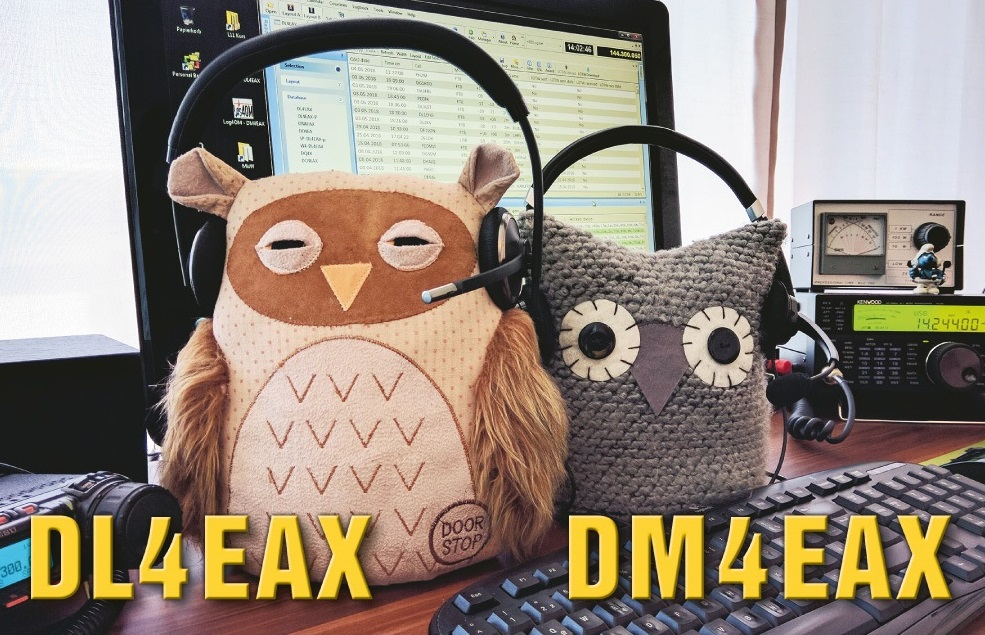
\includegraphics[width=0.85\textwidth]{foto/12}
    \caption{\scriptsize Gemeinsame QSL-Karte von DL4EAX und DM4EAX (Vorderseite)}
    \label{n_qsl_karten_vorderseite}
\end{figure}

   \end{column}
\end{columns}

\end{frame}

\begin{frame}
\only<1>{
\begin{QQuestion}{BG104}{Eine QSL-Karte ist~...}{eine Reservierungsbestätigung für die Teilnahme an einer Amateurfunkrunde. Sie sichert dem Funkamateur einen Listenplatz in der Runde.}
{die Bescheinigung über die Mitgliedschaft in einer Amateurfunkvereinigung.}
{eine Landkarte, in der Standorte für ortsgebundene Funkwettbewerbe eingezeichnet sind.}
{die Bestätigung einer Amateurfunkverbindung. Sie dient z. B. als Beleg bei der Beantragung von Amateurfunk-Diplomen.}
\end{QQuestion}

}
\only<2>{
\begin{QQuestion}{BG104}{Eine QSL-Karte ist~...}{eine Reservierungsbestätigung für die Teilnahme an einer Amateurfunkrunde. Sie sichert dem Funkamateur einen Listenplatz in der Runde.}
{die Bescheinigung über die Mitgliedschaft in einer Amateurfunkvereinigung.}
{eine Landkarte, in der Standorte für ortsgebundene Funkwettbewerbe eingezeichnet sind.}
{\textbf{\textcolor{DARCgreen}{die Bestätigung einer Amateurfunkverbindung. Sie dient z. B. als Beleg bei der Beantragung von Amateurfunk-Diplomen.}}}
\end{QQuestion}

}
\end{frame}

\begin{frame}
\frametitle{Angaben}

\begin{figure}
    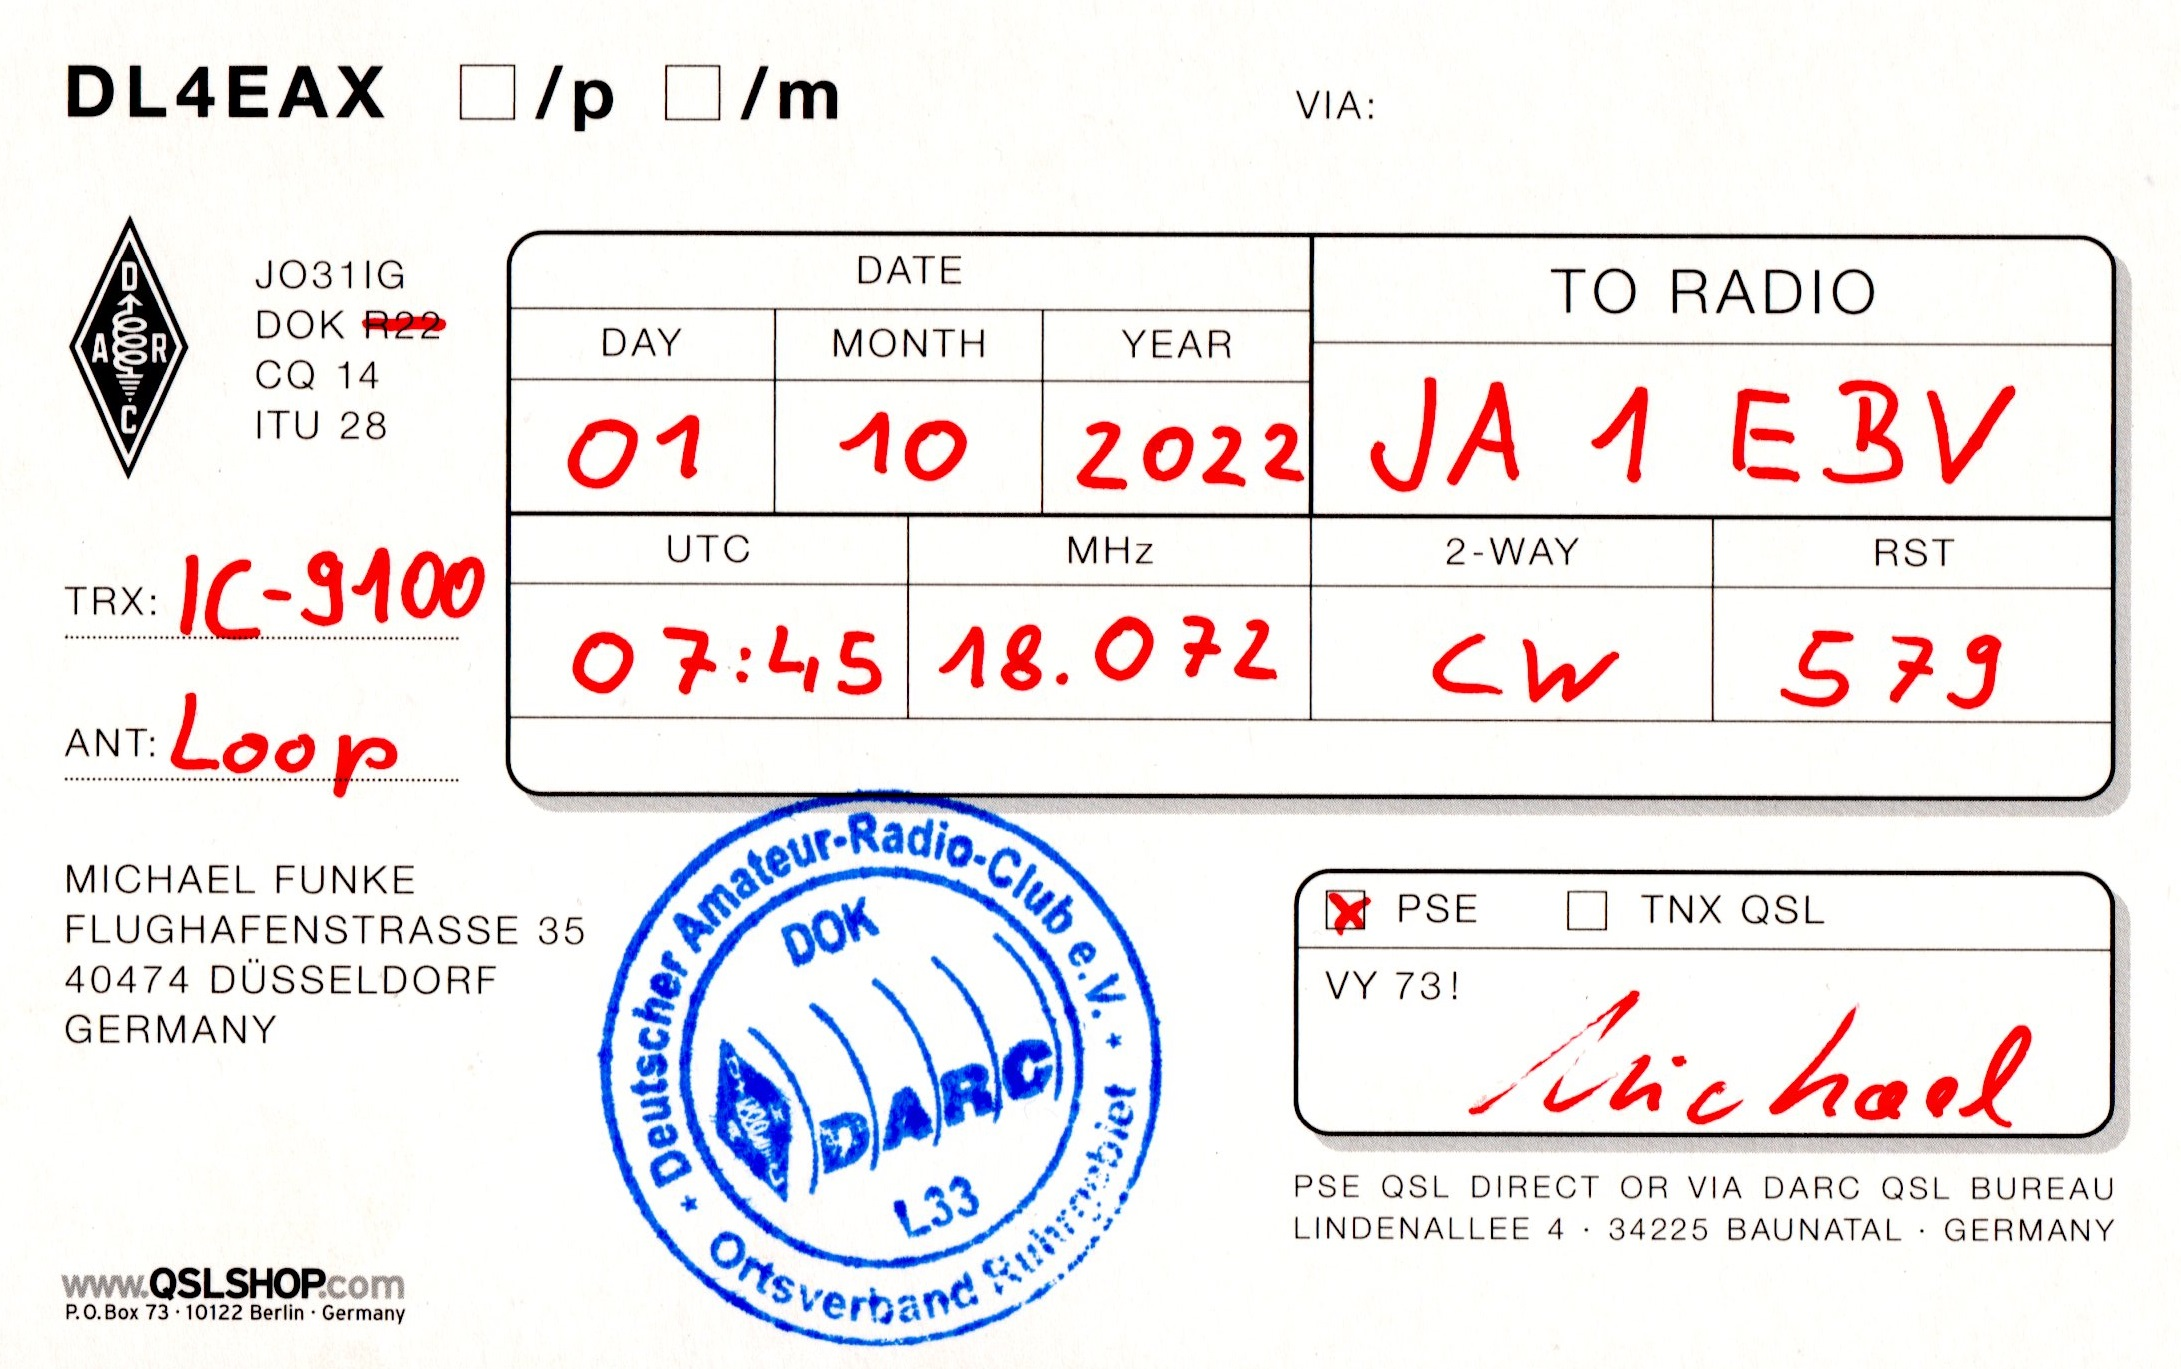
\includegraphics[width=0.85\textwidth]{foto/62}
    \caption{\scriptsize Beispiel für eine QSL-Karte, ausgestellt von DL4EAX zur Bestätigung einer Verbindung mit der Station JA1EBV}
    \label{n_qsl_karten_rueckseite_2}
\end{figure}
\end{frame}

\begin{frame}Eine QSL-Karte sollte mindestens folgende Angaben enthalten:

\begin{itemize}
  \item Datum
  \item Uhrzeit in UTC
  \item Eigenes Rufzeichen
  \item Rufzeichen der Gegenstation
  \item Genutzte Frequenz oder Frequenzband
  \item Verwendetes Übertragungsverfahren
  \item Gegebener Rapport
  \end{itemize}

\end{frame}

\begin{frame}
\only<1>{
\begin{QQuestion}{BG105}{Welche Angaben sollten QSL-Karten \underline{mindestens} enthalten?}{Verwendetes Rufzeichen, Datum und Uhrzeit der Funkverbindung in UTC, Frequenz, Übertragungsverfahren, Signal-Rapport sowie den eigenen Namen, Standort, Locator, die eigene Sendeleistung und Angaben zur eingesetzten technischen Ausrüstung}
{Verwendetes Rufzeichen, Rufzeichen der Gegenstation, Datum und Uhrzeit der Funkverbindung in UTC, Band, Übertragungsverfahren und Signal-Rapport}
{Rufzeichen der Gegenstation, Datum und Uhrzeit der Funkverbindung in UTC, genaue Frequenz, Übertragungsverfahren, Signal-Rapport und weitere übliche Angaben wie den eigenen Namen, Standort, Locator und die eigene Sendeleistung}
{Rufzeichen der Gegenstation, Datum und Uhrzeit der Funkverbindung in UTC, Frequenz, Übertragungsverfahren, Angaben über das Funkwetter und die Unterschrift des Operators}
\end{QQuestion}

}
\only<2>{
\begin{QQuestion}{BG105}{Welche Angaben sollten QSL-Karten \underline{mindestens} enthalten?}{Verwendetes Rufzeichen, Datum und Uhrzeit der Funkverbindung in UTC, Frequenz, Übertragungsverfahren, Signal-Rapport sowie den eigenen Namen, Standort, Locator, die eigene Sendeleistung und Angaben zur eingesetzten technischen Ausrüstung}
{\textbf{\textcolor{DARCgreen}{Verwendetes Rufzeichen, Rufzeichen der Gegenstation, Datum und Uhrzeit der Funkverbindung in UTC, Band, Übertragungsverfahren und Signal-Rapport}}}
{Rufzeichen der Gegenstation, Datum und Uhrzeit der Funkverbindung in UTC, genaue Frequenz, Übertragungsverfahren, Signal-Rapport und weitere übliche Angaben wie den eigenen Namen, Standort, Locator und die eigene Sendeleistung}
{Rufzeichen der Gegenstation, Datum und Uhrzeit der Funkverbindung in UTC, Frequenz, Übertragungsverfahren, Angaben über das Funkwetter und die Unterschrift des Operators}
\end{QQuestion}

}
\end{frame}

\begin{frame}
\only<1>{
\begin{QQuestion}{BG106}{Was sollten Sie bei der Eintragung von Uhrzeiten in QSL-Karten beachten? Sie sollten in~...}{der Ortszeit des Funkpartners eingetragen werden, damit es zu keinen Verwechselungen kommt.}
{der eigenen Ortszeit eingetragen werden, um den deutschen Vorschriften zu genügen.}
{der koordinierten Weltzeit (UTC) eingetragen werden, um Funkpartnern im Ausland das Auffinden im Logbuch zu erleichtern.}
{der eigenen Ortszeit und zusätzlich in der Ortszeit des Funkpartners eingetragen werden, um sowohl den deutschen Vorschriften zu genügen als auch Funkpartnern im Ausland das Auffinden im Logbuch zu erleichtern.}
\end{QQuestion}

}
\only<2>{
\begin{QQuestion}{BG106}{Was sollten Sie bei der Eintragung von Uhrzeiten in QSL-Karten beachten? Sie sollten in~...}{der Ortszeit des Funkpartners eingetragen werden, damit es zu keinen Verwechselungen kommt.}
{der eigenen Ortszeit eingetragen werden, um den deutschen Vorschriften zu genügen.}
{\textbf{\textcolor{DARCgreen}{der koordinierten Weltzeit (UTC) eingetragen werden, um Funkpartnern im Ausland das Auffinden im Logbuch zu erleichtern.}}}
{der eigenen Ortszeit und zusätzlich in der Ortszeit des Funkpartners eingetragen werden, um sowohl den deutschen Vorschriften zu genügen als auch Funkpartnern im Ausland das Auffinden im Logbuch zu erleichtern.}
\end{QQuestion}

}
\end{frame}

\begin{frame}
\only<1>{
\begin{QQuestion}{BG107}{Welche Uhrzeit tragen Sie in die QSL-Karte ein, wenn Sie um 15:30 MEZ ein QSO hatten?}{14:30 UTC}
{13:30 UTC}
{17:30 UTC}
{16:30 UTC}
\end{QQuestion}

}
\only<2>{
\begin{QQuestion}{BG107}{Welche Uhrzeit tragen Sie in die QSL-Karte ein, wenn Sie um 15:30 MEZ ein QSO hatten?}{\textbf{\textcolor{DARCgreen}{14:30 UTC}}}
{13:30 UTC}
{17:30 UTC}
{16:30 UTC}
\end{QQuestion}

}
\end{frame}

\begin{frame}
\only<1>{
\begin{QQuestion}{BG108}{Welche Uhrzeit tragen Sie in die QSL-Karte ein, wenn Sie um 13:30 MESZ eine Funkverbindung hatten?}{11:30 UTC}
{13:30 UTC}
{12:30 UTC}
{14:30 UTC}
\end{QQuestion}

}
\only<2>{
\begin{QQuestion}{BG108}{Welche Uhrzeit tragen Sie in die QSL-Karte ein, wenn Sie um 13:30 MESZ eine Funkverbindung hatten?}{\textbf{\textcolor{DARCgreen}{11:30 UTC}}}
{13:30 UTC}
{12:30 UTC}
{14:30 UTC}
\end{QQuestion}

}
\end{frame}

\begin{frame}
\frametitle{Vermittlung von QSL-Karten}
\begin{itemize}
  \item Über teilnehmende Amateurfunkverbände in den Ländern
  \item via Vermittlungsbüro -- international \enquote{Bureau}
  \item Weltweites alternatives Postnetz
  \item In Deutschland bietet das der DARC e.V. für Mitglieder kostenlos an
  \end{itemize}

\end{frame}

\begin{frame}
\frametitle{Callbooks}
\begin{itemize}
  \item Adressen in internationalen Amateurfunk-Rufzeichenlisten (Callbook)
  \item Oder im Internet
  \item Es gibt \enquote{QSL-Manager}, die für andere Stationen den Versand übernehmen
  \end{itemize}

\end{frame}

\begin{frame}
\only<1>{
\begin{QQuestion}{BG110}{Wo können Sie die Anschriften von ausländischen Funkamateuren finden, denen Sie die QSL-Karte direkt zusenden möchten?}{Ich finde diese in der VO Funk.}
{Ich finde diese in der Amateurfunk-Rufzeichenliste auf den Internetseiten der Bundesnetzagentur.}
{Ich finde diese in der internationalen Amateurfunk-Rufzeichenliste (Callbook) oder aus Informationen des Internets.}
{Ich finde diese im internationalen Telefonbuch.}
\end{QQuestion}

}
\only<2>{
\begin{QQuestion}{BG110}{Wo können Sie die Anschriften von ausländischen Funkamateuren finden, denen Sie die QSL-Karte direkt zusenden möchten?}{Ich finde diese in der VO Funk.}
{Ich finde diese in der Amateurfunk-Rufzeichenliste auf den Internetseiten der Bundesnetzagentur.}
{\textbf{\textcolor{DARCgreen}{Ich finde diese in der internationalen Amateurfunk-Rufzeichenliste (Callbook) oder aus Informationen des Internets.}}}
{Ich finde diese im internationalen Telefonbuch.}
\end{QQuestion}

}
\end{frame}

\begin{frame}
\only<1>{
\begin{QQuestion}{BG109}{HZ1HZ sagte Ihnen \glqq QSL via K8PYD\grqq{}. Was würden Sie tun, um die QSL-Karte von HZ1HZ zu erhalten?}{Ich warte, bis HZ1HZ die Karte an K8PYD geschickt hat.}
{Ich muss meine QSL-Karte via HZ1HZ senden, weil K8PYD der QSO-Partner war.}
{Ich schaue im Callbook nach der Adresse von HZ1HZ und schicke die Karte direkt.}
{Ich sende meine QSL-Karte via K8PYD, weil dieser der QSL-Manager von HZ1HZ ist.}
\end{QQuestion}

}
\only<2>{
\begin{QQuestion}{BG109}{HZ1HZ sagte Ihnen \glqq QSL via K8PYD\grqq{}. Was würden Sie tun, um die QSL-Karte von HZ1HZ zu erhalten?}{Ich warte, bis HZ1HZ die Karte an K8PYD geschickt hat.}
{Ich muss meine QSL-Karte via HZ1HZ senden, weil K8PYD der QSO-Partner war.}
{Ich schaue im Callbook nach der Adresse von HZ1HZ und schicke die Karte direkt.}
{\textbf{\textcolor{DARCgreen}{Ich sende meine QSL-Karte via K8PYD, weil dieser der QSL-Manager von HZ1HZ ist.}}}
\end{QQuestion}

}
\end{frame}

\begin{frame}
\frametitle{Elektronische QSL-Karten}
\begin{itemize}
  \item Papierlose Alternativen
  \item Elektronische Logbücher lassen sich hochladen
  \item Nur wenige Plattformen werden für Diplome anerkannt
  \end{itemize}
\end{frame}

\begin{frame}
\only<1>{
\begin{QQuestion}{BG111}{Welche Alternativen zur QSL-Karte sind üblich? Bestätigung von Funkverbindungen durch~...}{elektronische QSL-Karten oder Logbuch-Upload}
{die BNetzA als unabhängige Stelle}
{das Intruder Monitoring der Amateurfunkverbände}
{Beurkundung durch einen Notar oder SWL-Fachanwalt}
\end{QQuestion}

}
\only<2>{
\begin{QQuestion}{BG111}{Welche Alternativen zur QSL-Karte sind üblich? Bestätigung von Funkverbindungen durch~...}{\textbf{\textcolor{DARCgreen}{elektronische QSL-Karten oder Logbuch-Upload}}}
{die BNetzA als unabhängige Stelle}
{das Intruder Monitoring der Amateurfunkverbände}
{Beurkundung durch einen Notar oder SWL-Fachanwalt}
\end{QQuestion}

}
\end{frame}%ENDCONTENT


\title{DARC Amateurfunklehrgang Klasse NEA}
\author{Digitale Übertragungsverfahren}
\institute{Deutscher Amateur Radio Club e.\,V.}
\begin{frame}
\maketitle
\end{frame}

\section{Analog vs. Digital}
\label{section:analog_vs_digital}
\begin{frame}%STARTCONTENT

\begin{columns}
    \begin{column}{0.48\textwidth}
    Bei der Informationsübertragung unterscheidet man grundsätzlich zwischen analogen und digitalen Verfahren.

\begin{itemize}
  \item \emph{Digital}: in Stufen, nur bestimmte Werte, keine Werte dazwischen
  \item \emph{Analog}: kontinuierlich, beliebige Zwischenwerte
  \end{itemize}

    \end{column}
   \begin{column}{0.48\textwidth}
       
\begin{figure}
    \DARCimage{0.85\linewidth}{411include}
    \caption{\scriptsize Digitales Signal (abgestuft)}
    \label{n_digital_einleitung_digitales_signal}
\end{figure}


\begin{figure}
    \DARCimage{0.85\linewidth}{408include}
    \caption{\scriptsize Analoges Signal (kontinuierlich)}
    \label{n_digital_einleitung_analoges_signal}
\end{figure}


   \end{column}
\end{columns}

\end{frame}%ENDCONTENT


\section{Binäres Zahlensystem}
\label{section:binaer}
\begin{frame}%STARTCONTENT

\begin{columns}
    \begin{column}{0.48\textwidth}
    \emph{Dezimalsystem}

\begin{itemize}
  \item Menschen sind es gewohnt, die zehn Ziffern von 0 bis 9 zu benutzen
  \item Man spricht von einem Zehner- oder Dezimalsystem
  \end{itemize}

    \end{column}
   \begin{column}{0.48\textwidth}
       \emph{Binärsystem}

\begin{itemize}
  \item Für Computer ist es hingegen einfacher mit nur 2 Ziffern zu arbeiten: Der 0 und der 1
  \item Dies entspricht zwei Zuständen: Beispielsweise ausgeschaltet und eingeschaltet oder auch 0 V und 5 V
  \end{itemize}

   \end{column}
\end{columns}

\end{frame}

\begin{frame}
\only<1>{
\begin{QQuestion}{EA201}{Was ist der Vorteil des binären Zahlensystems gegenüber dem dezimalen Zahlensystem in elektronischen Schaltungen?}{Die Genauigkeit des binären Systems (mit zwei Ziffern) ist um den Faktor 5 höher als die des Dezimalsystems (mit 10 Ziffern).}
{Die binären Ziffern 0 und 1 können als zwei elektrische Zustände dargestellt und dadurch einfach mittels Schaltelementen (z.~B. Transistoren) verarbeitet werden.}
{Der Zwischenbereich zwischen 0 und 1 kann von analogen Verstärkerschaltungen mit hoher Genauigkeit abgebildet werden.}
{Je Ziffer kann mehr als ein Bit an Information übertragen werden (1 binäre Ziffer erlaubt die Übertragung von 8 Dezimalziffern).}
\end{QQuestion}

}
\only<2>{
\begin{QQuestion}{EA201}{Was ist der Vorteil des binären Zahlensystems gegenüber dem dezimalen Zahlensystem in elektronischen Schaltungen?}{Die Genauigkeit des binären Systems (mit zwei Ziffern) ist um den Faktor 5 höher als die des Dezimalsystems (mit 10 Ziffern).}
{\textbf{\textcolor{DARCgreen}{Die binären Ziffern 0 und 1 können als zwei elektrische Zustände dargestellt und dadurch einfach mittels Schaltelementen (z.~B. Transistoren) verarbeitet werden.}}}
{Der Zwischenbereich zwischen 0 und 1 kann von analogen Verstärkerschaltungen mit hoher Genauigkeit abgebildet werden.}
{Je Ziffer kann mehr als ein Bit an Information übertragen werden (1 binäre Ziffer erlaubt die Übertragung von 8 Dezimalziffern).}
\end{QQuestion}

}
\end{frame}

\begin{frame}\begin{itemize}
  \item Mit einem Bit sind zwei Werte möglich (0 und 1)
  \item Mit zwei Bits schon vier (00, 01, 10 und 11) und mit jedem weiteren Bit jeweils doppelt so viele
  \item Mathematisch ausgedrückt: Mit n Bits lassen sich 2<sup>n</sup> verschiedene Zahlen darstellen
  \item Neben Binärzahl wird auch Dualzahl gesagt
  \end{itemize}
\end{frame}

\begin{frame}
\only<1>{
\begin{QQuestion}{EA202}{Wie viele unterschiedliche Zustände können mit einer Dualzahl dargestellt werden, die aus einer Folge von \qty{3}{\bit} besteht?}{8}
{4}
{6}
{16}
\end{QQuestion}

}
\only<2>{
\begin{QQuestion}{EA202}{Wie viele unterschiedliche Zustände können mit einer Dualzahl dargestellt werden, die aus einer Folge von \qty{3}{\bit} besteht?}{\textbf{\textcolor{DARCgreen}{8}}}
{4}
{6}
{16}
\end{QQuestion}

}
\end{frame}

\begin{frame}
\only<1>{
\begin{QQuestion}{EA203}{Wie viele unterschiedliche Zustände können mit einer Dualzahl dargestellt werden, die aus einer Folge von \qty{4}{\bit} besteht?}{16}
{4}
{6}
{8}
\end{QQuestion}

}
\only<2>{
\begin{QQuestion}{EA203}{Wie viele unterschiedliche Zustände können mit einer Dualzahl dargestellt werden, die aus einer Folge von \qty{4}{\bit} besteht?}{\textbf{\textcolor{DARCgreen}{16}}}
{4}
{6}
{8}
\end{QQuestion}

}
\end{frame}

\begin{frame}
\only<1>{
\begin{QQuestion}{EA204}{Wie viele unterschiedliche Werte können mit einer fünfstelligen Dualzahl dargestellt werden?}{5}
{32}
{64}
{128}
\end{QQuestion}

}
\only<2>{
\begin{QQuestion}{EA204}{Wie viele unterschiedliche Werte können mit einer fünfstelligen Dualzahl dargestellt werden?}{5}
{\textbf{\textcolor{DARCgreen}{32}}}
{64}
{128}
\end{QQuestion}

}
\end{frame}

\begin{frame}
\frametitle{Umwandlung}
Binärzahlen in Dezimale Zahlen am Beispiel von 10001110

\begin{table}
\begin{DARCtabular}{cccccccc}
      &  &  &  &  &  &  &   \\
     2<sup>7</sup>  & 2<sup>6</sup>  & 2<sup>5</sup>  & 2<sup>4</sup>  & 2<sup>3</sup>  & 2<sup>2</sup>  & 2<sup>1</sup>  & 2<sup>0</sup>   \\
     128  & 64  & 32  & 16  & 8  & 4  & 2  & 1   \\
     1  & 0  & 0  & 0  & 1  & 1  & 1  & 0   \\
\end{DARCtabular}
\caption{Stellenwerte der achtstelligen Dualzahl 10001110}
\label{binar_stellenwert_dual}
\end{table}
    \pause
    128 + 8 + 4 + 2 = 142

\end{frame}

\begin{frame}
\only<1>{
\begin{QQuestion}{EA205}{Berechnen Sie den dezimalen Wert der Dualzahl 01001110. Die Dezimalzahl lautet:}{156}
{78}
{142}
{248}
\end{QQuestion}

}
\only<2>{
\begin{QQuestion}{EA205}{Berechnen Sie den dezimalen Wert der Dualzahl 01001110. Die Dezimalzahl lautet:}{156}
{\textbf{\textcolor{DARCgreen}{78}}}
{142}
{248}
\end{QQuestion}

}
\end{frame}

\begin{frame}
\only<1>{
\begin{QQuestion}{EA206}{Berechnen Sie den dezimalen Wert der Dualzahl 10001110. Die Dezimalzahl lautet:}{78}
{142}
{156}
{248}
\end{QQuestion}

}
\only<2>{
\begin{QQuestion}{EA206}{Berechnen Sie den dezimalen Wert der Dualzahl 10001110. Die Dezimalzahl lautet:}{78}
{\textbf{\textcolor{DARCgreen}{142}}}
{156}
{248}
\end{QQuestion}

}
\end{frame}

\begin{frame}
\only<1>{
\begin{QQuestion}{EA207}{Berechnen Sie den dezimalen Wert der Dualzahl 10011100. Die Dezimalzahl lautet:}{78}
{142}
{156}
{248}
\end{QQuestion}

}
\only<2>{
\begin{QQuestion}{EA207}{Berechnen Sie den dezimalen Wert der Dualzahl 10011100. Die Dezimalzahl lautet:}{78}
{142}
{\textbf{\textcolor{DARCgreen}{156}}}
{248}
\end{QQuestion}

}
\end{frame}

\begin{frame}
\only<1>{
\begin{QQuestion}{EA208}{Berechnen Sie den dezimalen Wert der Dualzahl 11111000. Die Dezimalzahl lautet:}{142}
{78}
{156}
{248}
\end{QQuestion}

}
\only<2>{
\begin{QQuestion}{EA208}{Berechnen Sie den dezimalen Wert der Dualzahl 11111000. Die Dezimalzahl lautet:}{142}
{78}
{156}
{\textbf{\textcolor{DARCgreen}{248}}}
\end{QQuestion}

}
\end{frame}%ENDCONTENT


\section{Morsetelegrafie}
\label{section:morsetelegrafie}
\begin{frame}%STARTCONTENT
\begin{itemize}
  \item Ein- und Ausschalten eines Trägers
  \item Einführung eines \emph{Morsealphabets} 1838 durch Samuel Morse, optimiert durch Friedrich Clemens Gerke
  \item Morseprüfung lange Zeit Vorschrift für Funkamateure auf Kurzwelle
  \item Seit Mitte der 1990er legen Länder fest, ob \emph{Morseprüfung} notwendig ist
  \item Erst seit 2003 ist die Morseprüfung in Deutschland freiwillig
  \end{itemize}

\end{frame}

\begin{frame}\begin{table}
\begin{DARCtabular}{clclcl}
    ~  &~   &~   &~   &~   &~    \\
     A  & \MorseDit\MorseDah  & K  & \MorseDah\MorseDit\MorseDah  & U  & \MorseDit\MorseDit\MorseDah   \\
     B  & \MorseDah\MorseDit\MorseDit\MorseDit  & L  & \MorseDit\MorseDah\MorseDit\MorseDit  & V  & \MorseDit\MorseDit\MorseDit\MorseDah   \\
     C  & \MorseDah\MorseDit\MorseDah\MorseDit  & M  & \MorseDah\MorseDah  & W  & \MorseDit\MorseDah\MorseDah   \\
     D  & \MorseDah\MorseDit\MorseDit  & N  & \MorseDah\MorseDit  & X  & \MorseDah\MorseDit\MorseDit\MorseDah   \\
     E  & \MorseDit  & O  & \MorseDah\MorseDah\MorseDah  & Y  & \MorseDah\MorseDit\MorseDah\MorseDah   \\
     F  & \MorseDit\MorseDit\MorseDah\MorseDit  & P  & \MorseDit\MorseDah\MorseDah\MorseDit  & Z  & \MorseDah\MorseDah\MorseDit\MorseDit   \\
     G  & \MorseDah\MorseDah\MorseDit  & Q  & \MorseDah\MorseDah\MorseDit\MorseDah  & Ä  & \MorseDit\MorseDah\MorseDit\MorseDah   \\
     H  & \MorseDit\MorseDit\MorseDit\MorseDit  & R  & \MorseDit\MorseDah\MorseDit  & Ö  & \MorseDah\MorseDah\MorseDah\MorseDit   \\
     I  & \MorseDit\MorseDit  & S  & \MorseDit\MorseDit\MorseDit  & Ü  & \MorseDit\MorseDit\MorseDah\MorseDah   \\
     J  & \MorseDit\MorseDah\MorseDah\MorseDah  & T  & \MorseDah  & ẞ  & \MorseDit\MorseDit\MorseDit\MorseDah\MorseDah\MorseDit\MorseDit   \\
\end{DARCtabular}
\caption{Morsecode (Buchstaben)}
\label{n_morsetelegrafie_morsecode_buchstaben}
\end{table}
\end{frame}

\begin{frame}\begin{table}
\begin{DARCtabular}{clclcl}
    ~   &~   &~   &~   &~   &~    \\
     0  & \MorseDah\MorseDah\MorseDah\MorseDah\MorseDah  & 5  & \MorseDit\MorseDit\MorseDit\MorseDit\MorseDit  & /  & \MorseDah\MorseDit\MorseDit\MorseDah\MorseDit   \\
     1  & \MorseDit\MorseDah\MorseDah\MorseDah\MorseDah  & 6  & \MorseDah\MorseDit\MorseDit\MorseDit\MorseDit  & .  & \MorseDit\MorseDah\MorseDit\MorseDah\MorseDit\MorseDah   \\
     2  & \MorseDit\MorseDit\MorseDah\MorseDah\MorseDah  & 7  & \MorseDah\MorseDah\MorseDit\MorseDit\MorseDit  & ,  & \MorseDah\MorseDah\MorseDit\MorseDit\MorseDah\MorseDah   \\
     3  & \MorseDit\MorseDit\MorseDit\MorseDah\MorseDah  & 8  & \MorseDah\MorseDah\MorseDah\MorseDit\MorseDit  & ?  & \MorseDit\MorseDit\MorseDah\MorseDah\MorseDit\MorseDit   \\
     4  & \MorseDit\MorseDit\MorseDit\MorseDit\MorseDah  & 9  & \MorseDah\MorseDah\MorseDah\MorseDah\MorseDit  & =  & \MorseDah\MorseDit\MorseDit\MorseDit\MorseDah   \\
\end{DARCtabular}
\caption{Morsecode (Ziffern und Satzzeichen)}
\label{n_morsetelegrafie_morsecode_ziffern_satzzeichen}
\end{table}
\begin{table}
\begin{DARCtabular}{ll}
    ~   &~    \\
     Unterbrechung (BK)  & \MorseDah\MorseDit\MorseDit\MorseDit\MorseDah\MorseDit\MorseDah   \\
     Ende des Durchgangs (AR)   & \MorseDit\MorseDah\MorseDit\MorseDah\MorseDit   \\
     Ende der Sendung (SK)  & \MorseDit\MorseDit\MorseDit\MorseDah\MorseDit\MorseDah   \\
     Korrektur  & \MorseDit\MorseDit\MorseDit\MorseDit\MorseDit\MorseDit\MorseDit\MorseDit   \\
\end{DARCtabular}
\caption{Morsecode (besondere Zeichen, Auswahl)}
\label{n_morsetelegrafie_morsecode_spezial}
\end{table}
\end{frame}

\begin{frame}
\only<1>{
\begin{QQuestion}{VA304}{Was ist in den Radio Regulations (RR) bezüglich der Morsequalifikation für Funkamateure festgelegt?}{Wer Frequenzen unter \qty{30}{\MHz} nutzen will, muss eine Morseprüfung ablegen.}
{Bei einer Sendeleistung von mehr als \qty{100}{\W} benötigt der Funkamateur den Nachweis einer erfolgreich abgelegten Morseprüfung.}
{Die nationale Verwaltung eines jeden Landes legt eigenständig fest, ob eine Morseprüfung erforderlich ist.}
{In den Radio Regulations (RR) werden bezüglich der Morsequalifikation keine Regelungen getroffen.}
\end{QQuestion}

}
\only<2>{
\begin{QQuestion}{VA304}{Was ist in den Radio Regulations (RR) bezüglich der Morsequalifikation für Funkamateure festgelegt?}{Wer Frequenzen unter \qty{30}{\MHz} nutzen will, muss eine Morseprüfung ablegen.}
{Bei einer Sendeleistung von mehr als \qty{100}{\W} benötigt der Funkamateur den Nachweis einer erfolgreich abgelegten Morseprüfung.}
{\textbf{\textcolor{DARCgreen}{Die nationale Verwaltung eines jeden Landes legt eigenständig fest, ob eine Morseprüfung erforderlich ist.}}}
{In den Radio Regulations (RR) werden bezüglich der Morsequalifikation keine Regelungen getroffen.}
\end{QQuestion}

}
\end{frame}%ENDCONTENT


\section{Computersteuerung}
\label{section:computersteuerung}
\begin{frame}%STARTCONTENT

\frametitle{Steuersignale}
\begin{columns}
    \begin{column}{0.48\textwidth}
    \begin{itemize}
  \item Übertragung von Audio- sowie Steuersignalen (CAT) zwischen Computer und Transceiver
  \item Z.B. Transceiver auf Sendung schalten und Signal vom Computer übertragen
  \end{itemize}

    \end{column}
   \begin{column}{0.48\textwidth}
       
\begin{figure}
    \DARCimage{0.85\linewidth}{630include}
    \caption{\scriptsize Beispiele für Verbindungen zwischen Computer und Funkgerät}
    \label{n_computersteuerung_verbindungen}
\end{figure}


   \end{column}
\end{columns}

\end{frame}

\begin{frame}
\frametitle{Datenanschluss}
\begin{itemize}
  \item Hinter dem Mikrofonanschluss im Funkgerät können Verstärker- und Filterstufen für Sprachübertragung liegen $\rightarrow$ ungeeignet für Datenübertragung
  \item Eigener Datenanschluss am Transceiver
  \item Lässt Signale vom Computer unverfälscht passieren
  \end{itemize}

\end{frame}

\begin{frame}
\only<1>{
\begin{QQuestion}{NF114}{Wie kann eine Verbindung zwischen Funkgerät und Computer für digitale Übertragungsverfahren (z.~B. FT8 oder WSPR) hergestellt werden?}{Der ALC-Anschluss des Funkgeräts wird mittels eines Hardware-Modems mit Audio- oder Datenanschlüssen des Computers verbunden.}
{Eine Audioverbindung (NF-Signal oder digital z.~B. per USB-Kabel) wird zwischen Computer und Funkgerät hergestellt oder es wird ein Hardware-Modem verwendet.}
{Es wird ein Software-Modem installiert und der ALC-Anschluss des Funkgeräts direkt mit dem Computer verbunden (ggf. auch mittels Adapter).}
{Der HF-Anschluss (z.~B. Antennenausgang) des Funkgeräts wird mittels eines Y-Kabels mit einer geeigneten Datenschnittstelle des Computers verbunden.}
\end{QQuestion}

}
\only<2>{
\begin{QQuestion}{NF114}{Wie kann eine Verbindung zwischen Funkgerät und Computer für digitale Übertragungsverfahren (z.~B. FT8 oder WSPR) hergestellt werden?}{Der ALC-Anschluss des Funkgeräts wird mittels eines Hardware-Modems mit Audio- oder Datenanschlüssen des Computers verbunden.}
{\textbf{\textcolor{DARCgreen}{Eine Audioverbindung (NF-Signal oder digital z.~B. per USB-Kabel) wird zwischen Computer und Funkgerät hergestellt oder es wird ein Hardware-Modem verwendet.}}}
{Es wird ein Software-Modem installiert und der ALC-Anschluss des Funkgeräts direkt mit dem Computer verbunden (ggf. auch mittels Adapter).}
{Der HF-Anschluss (z.~B. Antennenausgang) des Funkgeräts wird mittels eines Y-Kabels mit einer geeigneten Datenschnittstelle des Computers verbunden.}
\end{QQuestion}

}
\end{frame}

\begin{frame}
\only<1>{
\begin{QQuestion}{NF116}{Manche Transceiver verfügen über eine sogenannte CAT-Schnittstelle. Dieser Anschluss dient dazu,~...}{mittels eines seriellen Kommunikationsprotokolls den Transceiver z.~B. mit einem Computer zu steuern oder Werte abzufragen, z.~B. Frequenz, Sendeleistung oder PTT.}
{durch Umgehung von Verstärker- und Filterstufen ein NF-Signal (z.~B. für DV oder POCSAG) möglichst verzerrungsfrei abzugreifen oder einzuspeisen.}
{das empfangene HF-Signal möglichst ungefiltert an einen Computer zur Weiterverarbeitung mittels digitaler Signalverarbeitung auszuleiten.}
{ohne weitere Beschaltung einen Drehwinkelgeber (Encoder) oder ein Potentiometer zur präzisen Frequenzeinstellung anzuschließen.}
\end{QQuestion}

}
\only<2>{
\begin{QQuestion}{NF116}{Manche Transceiver verfügen über eine sogenannte CAT-Schnittstelle. Dieser Anschluss dient dazu,~...}{\textbf{\textcolor{DARCgreen}{mittels eines seriellen Kommunikationsprotokolls den Transceiver z.~B. mit einem Computer zu steuern oder Werte abzufragen, z.~B. Frequenz, Sendeleistung oder PTT.}}}
{durch Umgehung von Verstärker- und Filterstufen ein NF-Signal (z.~B. für DV oder POCSAG) möglichst verzerrungsfrei abzugreifen oder einzuspeisen.}
{das empfangene HF-Signal möglichst ungefiltert an einen Computer zur Weiterverarbeitung mittels digitaler Signalverarbeitung auszuleiten.}
{ohne weitere Beschaltung einen Drehwinkelgeber (Encoder) oder ein Potentiometer zur präzisen Frequenzeinstellung anzuschließen.}
\end{QQuestion}

}
\end{frame}

\begin{frame}
\only<1>{
\begin{QQuestion}{NF117}{Welcher unerwünschte Effekt kann eintreten, wenn ein Funkgerät mittels Computer gesteuert wird?}{Der Computer kann wie ein Elektrolytkondensator im Antennenkreis wirken und somit die Sendefrequenz verschieben.}
{Der Vorverstärker ist außer Funktion, wodurch Nachbarkanäle und Frequenzen in anderen Bändern gestört werden könnten.}
{Die automatische Pegelregelung (ALC) könnte ausgelöst werden und andere digitale Geräte stören.}
{Das Funkgerät könnte unerwartet auf Sendung schalten und somit unerwünschte Aussendungen verursachen oder Menschen in Gefahr bringen.}
\end{QQuestion}

}
\only<2>{
\begin{QQuestion}{NF117}{Welcher unerwünschte Effekt kann eintreten, wenn ein Funkgerät mittels Computer gesteuert wird?}{Der Computer kann wie ein Elektrolytkondensator im Antennenkreis wirken und somit die Sendefrequenz verschieben.}
{Der Vorverstärker ist außer Funktion, wodurch Nachbarkanäle und Frequenzen in anderen Bändern gestört werden könnten.}
{Die automatische Pegelregelung (ALC) könnte ausgelöst werden und andere digitale Geräte stören.}
{\textbf{\textcolor{DARCgreen}{Das Funkgerät könnte unerwartet auf Sendung schalten und somit unerwünschte Aussendungen verursachen oder Menschen in Gefahr bringen.}}}
\end{QQuestion}

}

\end{frame}

\begin{frame}
\only<1>{
\begin{QQuestion}{NF115}{Manche FM-Transceiver verfügen über einen analogen Datenanschluss (z.~B. mit DATA beschriftet oder als 9600-Port bezeichnet). Dieser dient im Wesentlichen dazu,~...}{durch Umgehung von Verstärker- und Filterstufen ein NF-Signal (z.~B. für DV oder POCSAG) möglichst verzerrungsfrei abzugreifen oder einzuspeisen.}
{mittels eines seriellen Kommunikationsprotokolls den Transceiver z.~B. mit einem Computer zu steuern und Werte abzufragen, z.~B. Frequenz, Sendeleistung oder PTT.}
{das empfangene HF-Signal möglichst ungefiltert an einen Computer auszuleiten und mittels digitaler Signalverarbeitung weiterzuverarbeiten.}
{ohne weitere Beschaltung einen Drehwinkelgeber (Encoder) oder ein Potentiometer zur präzisen Frequenzeinstellung anzuschließen.}
\end{QQuestion}

}
\only<2>{
\begin{QQuestion}{NF115}{Manche FM-Transceiver verfügen über einen analogen Datenanschluss (z.~B. mit DATA beschriftet oder als 9600-Port bezeichnet). Dieser dient im Wesentlichen dazu,~...}{\textbf{\textcolor{DARCgreen}{durch Umgehung von Verstärker- und Filterstufen ein NF-Signal (z.~B. für DV oder POCSAG) möglichst verzerrungsfrei abzugreifen oder einzuspeisen.}}}
{mittels eines seriellen Kommunikationsprotokolls den Transceiver z.~B. mit einem Computer zu steuern und Werte abzufragen, z.~B. Frequenz, Sendeleistung oder PTT.}
{das empfangene HF-Signal möglichst ungefiltert an einen Computer auszuleiten und mittels digitaler Signalverarbeitung weiterzuverarbeiten.}
{ohne weitere Beschaltung einen Drehwinkelgeber (Encoder) oder ein Potentiometer zur präzisen Frequenzeinstellung anzuschließen.}
\end{QQuestion}

}
\end{frame}%ENDCONTENT


\section{Funkfernschreiben}
\label{section:funkfernschreiben}
\begin{frame}%STARTCONTENT

\frametitle{Funkfernschreiber}
\begin{columns}
    \begin{column}{0.48\textwidth}
    
\begin{figure}
    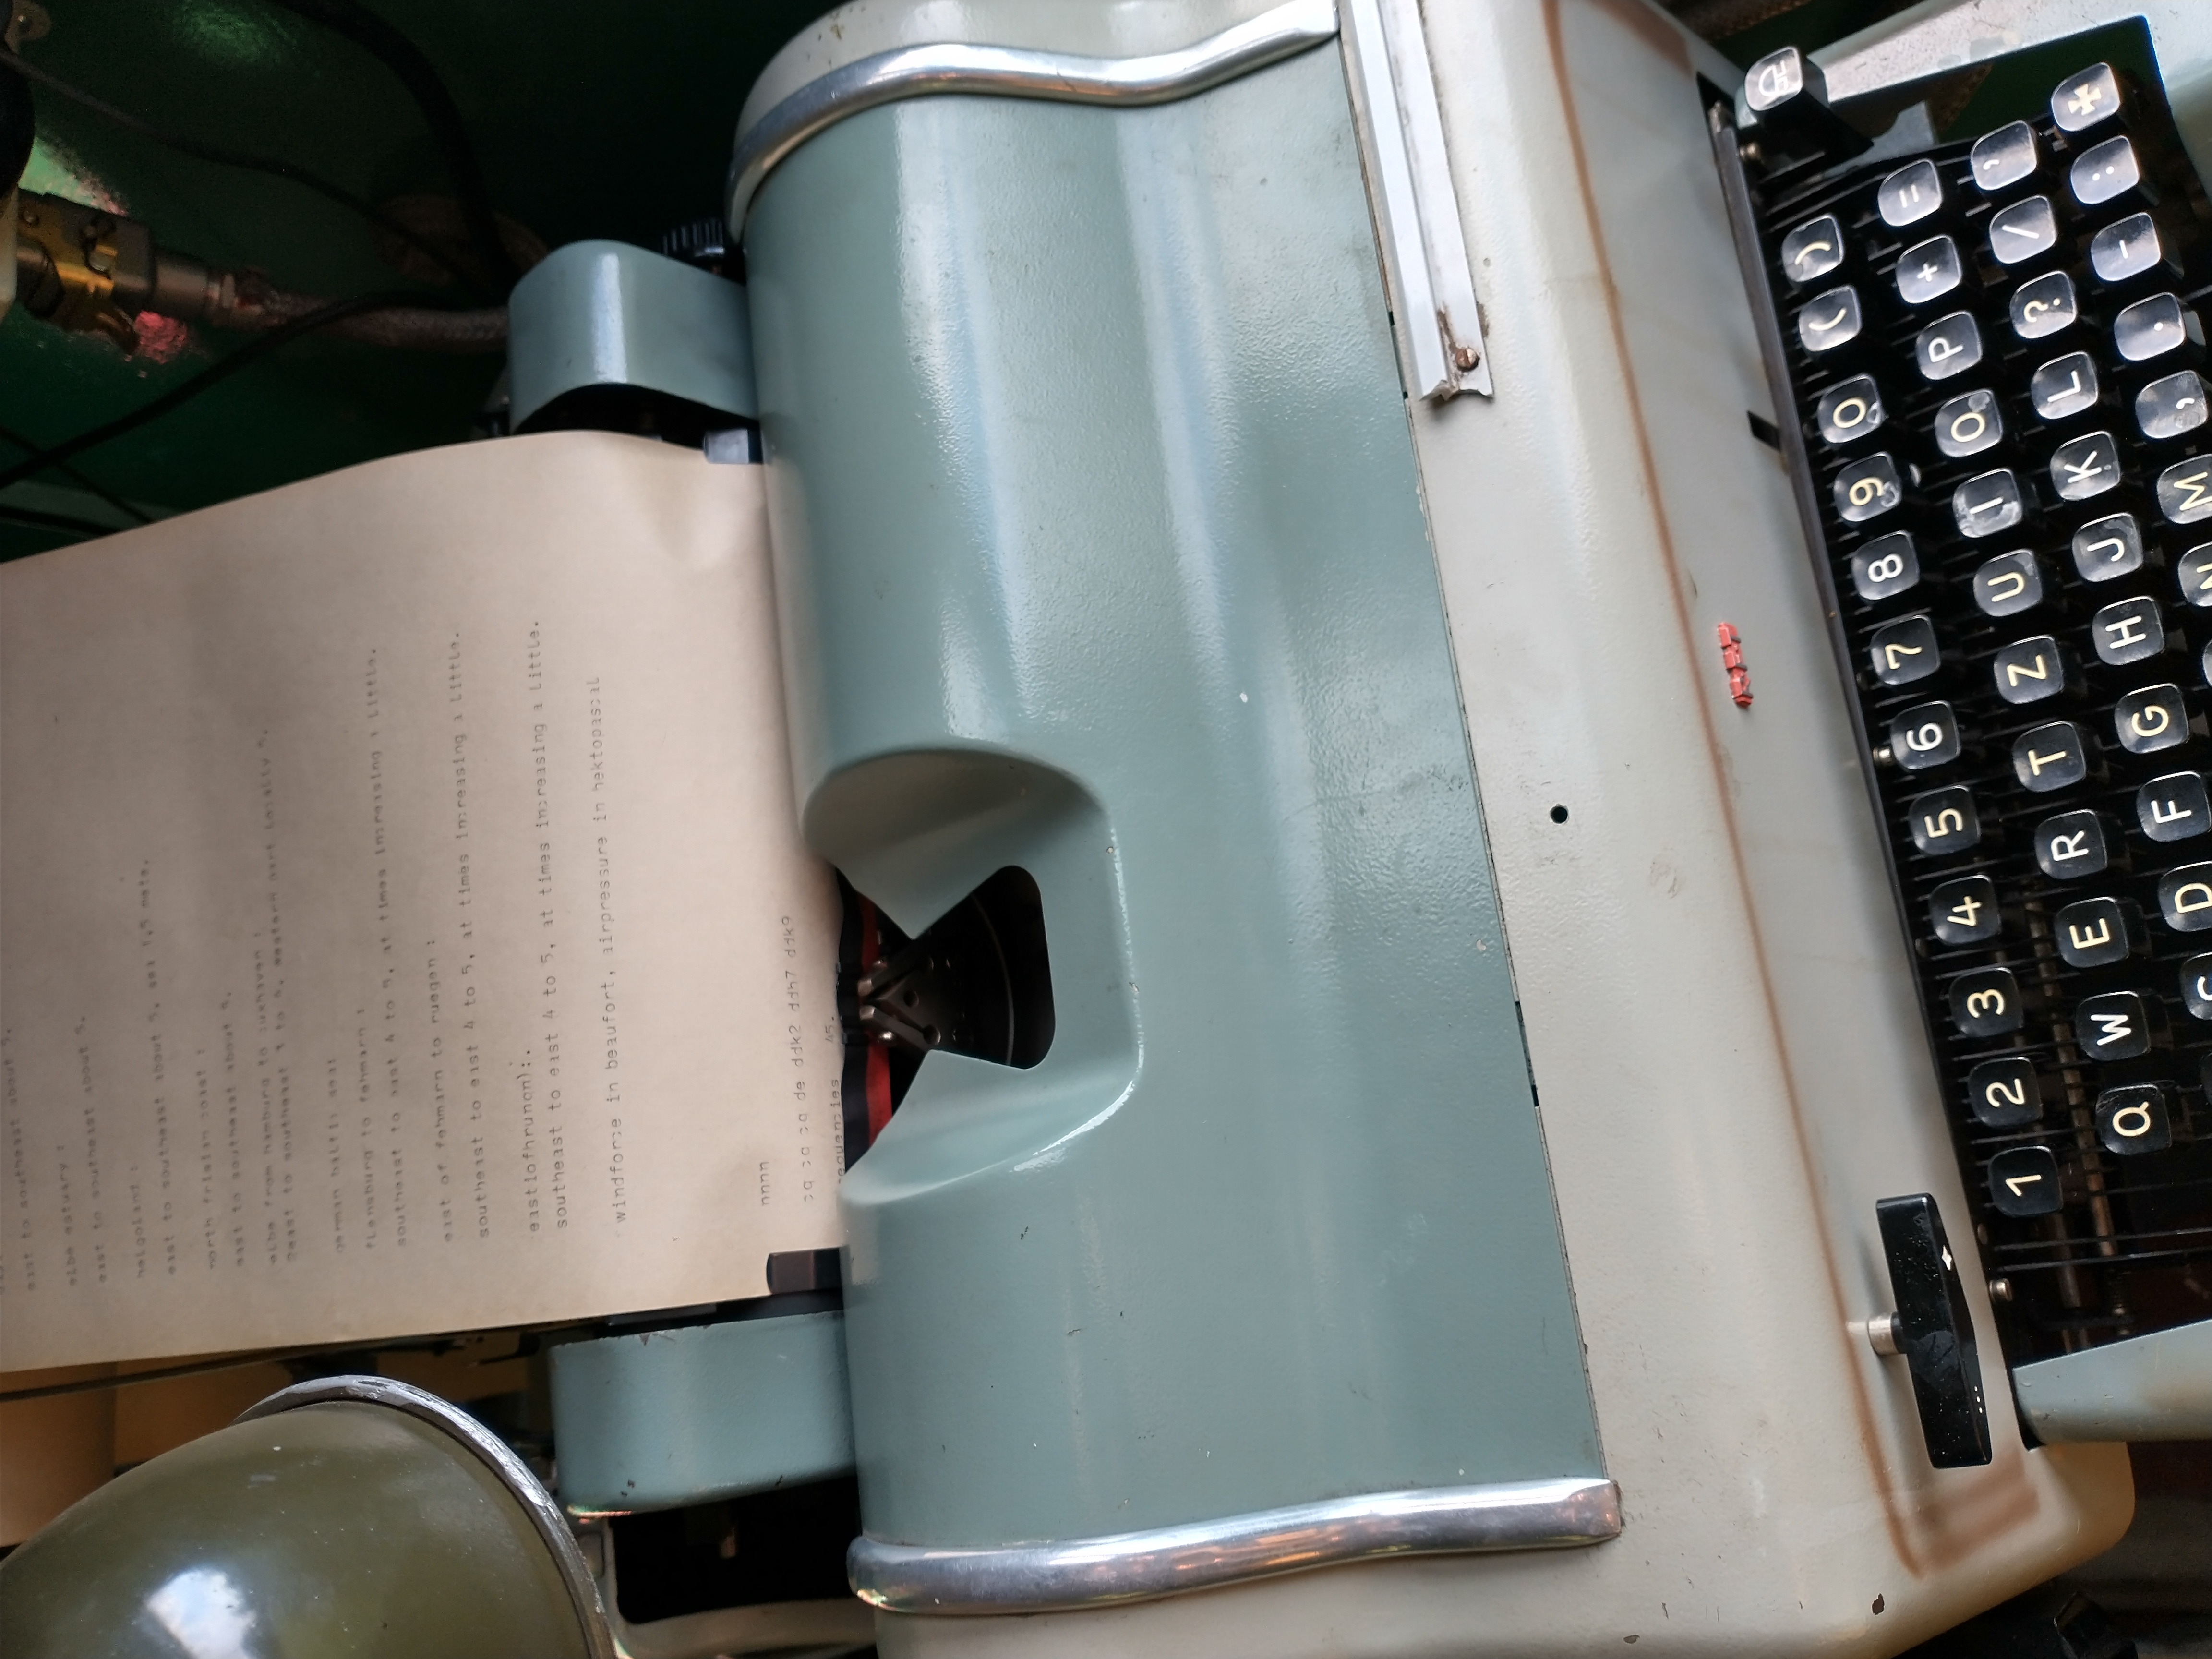
\includegraphics[width=0.85\textwidth]{foto/92}
    \caption{\scriptsize Funkfernschreiber}
    \label{n_computersteuerung_funkfernschreiber}
\end{figure}

    \end{column}
   \begin{column}{0.48\textwidth}
       Die Abkürzung RTTY stammt von \emph{radio teletype}


   \end{column}
\end{columns}

\end{frame}

\begin{frame}
\frametitle{Betrieb}
\begin{columns}
    \begin{column}{0.48\textwidth}
    \begin{itemize}
  \item Beide Funkpartner nutzen das gleiche Übertragungsverfahren (z.B. JS8, PSK, RTTY)
  \item Gleiche Parameter müssen gesetzt sein
  \end{itemize}

    \end{column}
   \begin{column}{0.48\textwidth}
       \begin{itemize}
  \item Verwendung von betrieblichen Abkürzungen und Q-Gruppen
  \item Mehr Informationsgehalt pro Zeiteinheit
  \end{itemize}

   \end{column}
\end{columns}

\end{frame}

\begin{frame}In einem Gespräch sieht dieses folgendermaßen aus:
    \pause\QSOown{CQ CQ CQ DE DL2AB DL2AB DL2AB PSE K}\pause\QSOother{DL2AB DE DL1PZ K}\pause\QSOown{DL1PZ DE DL2AB = UR RST 599 599 = DL1PZ DE DL2AB K}\pause\QSOother{DL2AB DE DL1PZ = TNX RPRT, UR 479 479 BK}\pause\QSOown{BK QSL = VY 73 DE DL2AB SK}\pause\QSOother{R 73 DE DL1PZ SK}

\end{frame}

\begin{frame}
\begin{columns}
    \begin{column}{0.48\textwidth}
    \begin{table}
\begin{DARCtabular}{ll}
     Abkz.  & Bedeutung   \\
     BK  & Unterbrechung der Sendung; Formlose Übergabe   \\
     CQ  & Allgemeiner Anruf (vom Englischen \enquote{Seek You})   \\
     DE  & von   \\
     K  & Aufforderung zum Senden   \\
     PSE  & Bitte (vom Englischen \enquote{Please})   \\
     QSL  & Ich bestätige den Empfang   \\
     R  & Received (Empfangsbestätigung)   \\
     RPRT  & Rapport (vom Englischen \enquote{Report})   \\
\end{DARCtabular}
\caption{Betriebliche Abkürzungen in der Telegrafie}
\label{n_funkfernschreiben_abkuerzungen_1}
\end{table}

    \end{column}
   \begin{column}{0.48\textwidth}
       \begin{table}
\begin{DARCtabular}{ll}
     Abkz.  & Bedeutung   \\
     RST  & RST-Rapport   \\
     SK  & Ende der Verbindung (vom Englischen \enquote{Silent Key})   \\
     TNX  & Danke (vom Englischen \enquote{Thanks})   \\
     UR  & du bist (im Sinne von \enquote{dein Signal ist}, vom Englischen \enquote{you are})   \\
     VY  & sehr (vom Englischen \enquote{very})   \\
     73  & viele Grüße   \\
     =  & Trennzeichen   \\
\end{DARCtabular}
\caption{Betriebliche Abkürzungen in der Telegrafie}
\label{n_funkfernschreiben_abkuerzungen_2}
\end{table}

   \end{column}
\end{columns}

\end{frame}

\begin{frame}Teil 1 unseres Beispiel-Gesprächs:
    \pause\QSOown{CQ CQ CQ DE DL2AB DL2AB DL2AB PSE K}\pause\QSOother{DL2AB DE DL1PZ K}
    \pause
    Allgemeiner Anruf von DL2AB -- Bitte Kommen!
    \pause
    DL2AB von DL1PZ -- Kommen!



\end{frame}

\begin{frame}Teil 2 unseres Beispiel-Gesprächs:
    \pause\QSOown{DL1PZ DE DL2AB = UR RST 599 599 = DL1PZ DE DL2AB K}\pause\QSOother{DL2AB DE DL1PZ = TNX RPRT, UR 479 479 BK}
    \pause
    DL1PZ von DL2AB. Dein Signal ist mit dem RST-Wert 599, ich wiederhole, 599. DL1PZ von DL2AB -- Kommen!
    \pause
    DL2AB von DL1PZ. Danke für den RST-Rapport, dein Signal ist 479, ich wiederhole, 479. Zurück zu dir!



\end{frame}

\begin{frame}Teil 3 unseres Beispiel-Gesprächs:
    \pause\QSOown{BK QSL = VY 73 DE DL2AB SK}\pause\QSOother{R 73 DE DL1PZ SK}
    \pause
    Hier bin ich wieder. Ich bestätige den Empfang. Sehr viele Grüße von DL2AB. Ende der Verbindung.
    \pause
    Verstanden. Viele Grüße von DL1PZ. Ende der Verbindung.



\end{frame}

\begin{frame}
\only<1>{
\begin{QQuestion}{NE401}{Was sollten Sie bei der Übertragung eines Textes per Funkfernschreiben beachten?}{Sende- und Empfangsstation müssen das gleiche Übertragungsverfahren (z. B. JS8, PSK, RTTY) und ggf. die gleichen Verfahrensparameter verwenden.}
{Sende- und Empfangsstation müssen die gleiche Zeitzoneneinstellung (z. B. Sommerzeit) aufweisen, damit die Übertragung erfolgreich sein kann.}
{Die Übertragung sollte bevorzugt während der Abend- und Nachtstunden stattfinden, da die Frequenzen tagsüber für Sprechverbindungen freigehalten werden.}
{Die Übertragung sollte bevorzugt mit einem schnellen Verfahren stattfinden, damit die Amateurfunkbänder nicht unnötig belastet werden.}
\end{QQuestion}

}
\only<2>{
\begin{QQuestion}{NE401}{Was sollten Sie bei der Übertragung eines Textes per Funkfernschreiben beachten?}{\textbf{\textcolor{DARCgreen}{Sende- und Empfangsstation müssen das gleiche Übertragungsverfahren (z. B. JS8, PSK, RTTY) und ggf. die gleichen Verfahrensparameter verwenden.}}}
{Sende- und Empfangsstation müssen die gleiche Zeitzoneneinstellung (z. B. Sommerzeit) aufweisen, damit die Übertragung erfolgreich sein kann.}
{Die Übertragung sollte bevorzugt während der Abend- und Nachtstunden stattfinden, da die Frequenzen tagsüber für Sprechverbindungen freigehalten werden.}
{Die Übertragung sollte bevorzugt mit einem schnellen Verfahren stattfinden, damit die Amateurfunkbänder nicht unnötig belastet werden.}
\end{QQuestion}

}
\end{frame}

\begin{frame}
\only<1>{
\begin{QQuestion}{BB101}{Warum werden insbesondere in der Telegrafie (z.~B. CW, JS8, RTTY) betriebliche Abkürzungen und Q-Gruppen verwendet?}{Sie werden als Kennung beim Amateurfunkpeilen genutzt, um die Sender zu kennzeichnen.}
{Der Informationsgehalt einer Aussendung wird verschleiert und ist damit für Unbeteiligte nicht verständlich.}
{Sie werden bei Verbindungen über Amateurfunksatelliten benutzt, um den Dopplereffekt durch kürzere Durchgänge zu vermeiden.}
{Der Betriebsablauf wird vereinfacht und der zu übertragende Informationsgehalt pro Zeiteinheit optimiert.}
\end{QQuestion}

}
\only<2>{
\begin{QQuestion}{BB101}{Warum werden insbesondere in der Telegrafie (z.~B. CW, JS8, RTTY) betriebliche Abkürzungen und Q-Gruppen verwendet?}{Sie werden als Kennung beim Amateurfunkpeilen genutzt, um die Sender zu kennzeichnen.}
{Der Informationsgehalt einer Aussendung wird verschleiert und ist damit für Unbeteiligte nicht verständlich.}
{Sie werden bei Verbindungen über Amateurfunksatelliten benutzt, um den Dopplereffekt durch kürzere Durchgänge zu vermeiden.}
{\textbf{\textcolor{DARCgreen}{Der Betriebsablauf wird vereinfacht und der zu übertragende Informationsgehalt pro Zeiteinheit optimiert.}}}
\end{QQuestion}

}
\end{frame}

\begin{frame}
\only<1>{
\begin{QQuestion}{BB110}{Was bedeutet \glqq R\grqq{} am Anfang eines Durchgangs in Telegrafie?}{Repeat (wiederhole)}
{Received (empfangen)}
{Rapport (Bericht)}
{Readability (Lesbarkeit)}
\end{QQuestion}

}
\only<2>{
\begin{QQuestion}{BB110}{Was bedeutet \glqq R\grqq{} am Anfang eines Durchgangs in Telegrafie?}{Repeat (wiederhole)}
{\textbf{\textcolor{DARCgreen}{Received (empfangen)}}}
{Rapport (Bericht)}
{Readability (Lesbarkeit)}
\end{QQuestion}

}
\end{frame}

\begin{frame}
\only<1>{
\begin{QQuestion}{BB109}{Was bedeutet \glqq K\grqq{} am Ende eines Durchgangs in Telegrafie?}{Unterbrechung der Sendung}
{Aufforderung zum Senden}
{Bitte warten}
{Beendigung des Funkverkehrs}
\end{QQuestion}

}
\only<2>{
\begin{QQuestion}{BB109}{Was bedeutet \glqq K\grqq{} am Ende eines Durchgangs in Telegrafie?}{Unterbrechung der Sendung}
{\textbf{\textcolor{DARCgreen}{Aufforderung zum Senden}}}
{Bitte warten}
{Beendigung des Funkverkehrs}
\end{QQuestion}

}
\end{frame}

\begin{frame}
\only<1>{
\begin{QQuestion}{BB108}{Was bedeutet die Betriebsabkürzung \glqq BK\grqq{} in Telegrafie?}{Beendigung des Funkverkehrs; wird auch zur formlosen Begrüßung genutzt}
{Alles richtig verstanden; wird auch zur schnellen Beendigung eines Funkkontakts genutzt}
{Bitte warten; wird auch zur schnellen Anforderung eines Rapports genutzt}
{Signal zur Unterbrechung einer laufenden Sendung; wird auch zur formlosen Übergabe genutzt}
\end{QQuestion}

}
\only<2>{
\begin{QQuestion}{BB108}{Was bedeutet die Betriebsabkürzung \glqq BK\grqq{} in Telegrafie?}{Beendigung des Funkverkehrs; wird auch zur formlosen Begrüßung genutzt}
{Alles richtig verstanden; wird auch zur schnellen Beendigung eines Funkkontakts genutzt}
{Bitte warten; wird auch zur schnellen Anforderung eines Rapports genutzt}
{\textbf{\textcolor{DARCgreen}{Signal zur Unterbrechung einer laufenden Sendung; wird auch zur formlosen Übergabe genutzt}}}
\end{QQuestion}

}
\end{frame}

\begin{frame}
\only<1>{
\begin{QQuestion}{BE112}{Wie gestalten Sie beispielsweise als \glqq DL2AB\grqq{} einen allgemeinen Anruf in Telegrafie?}{CQ CQ CQ DE DL2AB DL2AB DL2AB pse k}
{CQ CQ CQ FRM DL2AB DL2AB DL2AB pse k}
{QRZ QRZ QRZ DE DL2AB DL2AB DL2AB pse k}
{CQ QRZ CQ QRZ CQ QRZ DE DL2AB DL2AB DL2AB pse k}
\end{QQuestion}

}
\only<2>{
\begin{QQuestion}{BE112}{Wie gestalten Sie beispielsweise als \glqq DL2AB\grqq{} einen allgemeinen Anruf in Telegrafie?}{\textbf{\textcolor{DARCgreen}{CQ CQ CQ DE DL2AB DL2AB DL2AB pse k}}}
{CQ CQ CQ FRM DL2AB DL2AB DL2AB pse k}
{QRZ QRZ QRZ DE DL2AB DL2AB DL2AB pse k}
{CQ QRZ CQ QRZ CQ QRZ DE DL2AB DL2AB DL2AB pse k}
\end{QQuestion}

}
\end{frame}

\begin{frame}
\frametitle{Morsetelegrafie}
\begin{itemize}
  \item Auf die richtige Geschwindigkeit achten
  \item Schnell gegebene Morsezeichen brauchen viel Übung zum Verstehen
  \item Gegenstelle nicht mit der Geschwindigkeit überfordern
  \item Faustregel: \emph{Nicht schneller geben, als man selbst aufnehmen kann}
  \end{itemize}

\end{frame}

\begin{frame}
\only<1>{
\begin{QQuestion}{BE117}{Mit welcher Geschwindigkeit sollten Sie einen Anruf in Morsetelegrafie beantworten? In der Regel antworte ich~...}{mit einem Gebetempo von maximal 60 CPM.}
{mit meiner gewohnten Geschwindigkeit.}
{genauso schnell oder langsamer als der Anruf.}
{mit dem höchsten Tempo, das ich fehlerfrei geben kann.}
\end{QQuestion}

}
\only<2>{
\begin{QQuestion}{BE117}{Mit welcher Geschwindigkeit sollten Sie einen Anruf in Morsetelegrafie beantworten? In der Regel antworte ich~...}{mit einem Gebetempo von maximal 60 CPM.}
{mit meiner gewohnten Geschwindigkeit.}
{\textbf{\textcolor{DARCgreen}{genauso schnell oder langsamer als der Anruf.}}}
{mit dem höchsten Tempo, das ich fehlerfrei geben kann.}
\end{QQuestion}

}
\end{frame}

\begin{frame}
\only<1>{
\begin{QQuestion}{BE118}{Was sollten Sie hinsichtlich der Geschwindigkeit bei Morsetelegrafie beachten? Ich gebe in der Regel~...}{nicht schneller, als ich auch aufnehmen kann, und passe mich an langsamere Stationen an.}
{im international festgelegten Einheitstempo von 12 WPM, um eine automatische Dekodierung zu ermöglichen.}
{so schnell ich kann, damit es nicht zu unnötigen Verzögerungen im Betriebsablauf kommt.}
{in dem Tempo, das mir am besten liegt. Andere müssen sich an mich anpassen.}
\end{QQuestion}

}
\only<2>{
\begin{QQuestion}{BE118}{Was sollten Sie hinsichtlich der Geschwindigkeit bei Morsetelegrafie beachten? Ich gebe in der Regel~...}{\textbf{\textcolor{DARCgreen}{nicht schneller, als ich auch aufnehmen kann, und passe mich an langsamere Stationen an.}}}
{im international festgelegten Einheitstempo von 12 WPM, um eine automatische Dekodierung zu ermöglichen.}
{so schnell ich kann, damit es nicht zu unnötigen Verzögerungen im Betriebsablauf kommt.}
{in dem Tempo, das mir am besten liegt. Andere müssen sich an mich anpassen.}
\end{QQuestion}

}
\end{frame}%ENDCONTENT


\section{Digimode per SSB}
\label{section:digimode_ssb}
\begin{frame}%STARTCONTENT

\frametitle{Bandbreite von Digimodes}
\begin{itemize}
  \item Im Gegensatz zur Sprache benötigen viele Digimodes weniger Bandbreite
  \item Z.B. BPSK31 mit \qty{31,25}{\hertz} oder FT8 mit \qty{50}{\hertz}
  \item Die erzeugten Töne werden mittels Kurzwelle in SSB moduliert
  \item Die Bandbreite des ausgestrahlten Signals bleibt dabei gleich
  \end{itemize}
\end{frame}

\begin{frame}
\only<1>{
\begin{QQuestion}{EE403}{Bei der Aussendung eines digitalen Signals mittels eines Funkgerätes in SSB-Einstellung beträgt die NF-Bandbreite des in das Funkgerät eingespeisten Signals \qty{50}{\Hz}. Wie groß ist die HF-Bandbreite?}{$\sqrt{2} \cdot$ \qty{50}{\Hz}}
{\qty{100}{\Hz}}
{\qty{25}{\Hz}}
{\qty{50}{\Hz}}
\end{QQuestion}

}
\only<2>{
\begin{QQuestion}{EE403}{Bei der Aussendung eines digitalen Signals mittels eines Funkgerätes in SSB-Einstellung beträgt die NF-Bandbreite des in das Funkgerät eingespeisten Signals \qty{50}{\Hz}. Wie groß ist die HF-Bandbreite?}{$\sqrt{2} \cdot$ \qty{50}{\Hz}}
{\qty{100}{\Hz}}
{\qty{25}{\Hz}}
{\textbf{\textcolor{DARCgreen}{\qty{50}{\Hz}}}}
\end{QQuestion}

}
\end{frame}

\begin{frame}
\only<1>{
\begin{QQuestion}{EE402}{Welche Modulation wird am Transceiver eingestellt, um ein schmalbandiges digitales Signal (z.~B. BPSK31 oder FT8), das per Audiosignal als NF eingespeist wird, unter Beibehaltung der Bandbreite in HF umzusetzen?}{Phasenmodulation (PM)}
{Frequenzmodulation (FM)}
{Amplitudenmodulation (AM)}
{Einseitenbandmodulation (SSB)}
\end{QQuestion}

}
\only<2>{
\begin{QQuestion}{EE402}{Welche Modulation wird am Transceiver eingestellt, um ein schmalbandiges digitales Signal (z.~B. BPSK31 oder FT8), das per Audiosignal als NF eingespeist wird, unter Beibehaltung der Bandbreite in HF umzusetzen?}{Phasenmodulation (PM)}
{Frequenzmodulation (FM)}
{Amplitudenmodulation (AM)}
{\textbf{\textcolor{DARCgreen}{Einseitenbandmodulation (SSB)}}}
\end{QQuestion}

}
\end{frame}

\begin{frame}
\frametitle{Empfang von Digimodes}
\begin{columns}
    \begin{column}{0.48\textwidth}
    \begin{itemize}
  \item Beim Empfang von SSB können in der üblichen Bandbreite von \qty{2,4}{\kilo\hertz} mehrere schmalbandige Digimodes empfangen werden
  \item FT8: \qty{2400}{\hertz}  $\div$  \qty{50}{\hertz} = max. 48 Signale
  \item BPSK31: \qty{2400}{\hertz}  $\div$  \qty{31,25}{\hertz} = max. 76 Signale
  \item Am Computer wird dann das gewünschte Digimode-Signal selektiert
  \end{itemize}

    \end{column}
   \begin{column}{0.48\textwidth}
       
\begin{figure}
    \DARCimage{0.85\linewidth}{718include}
    \caption{\scriptsize Wasserfalldiagramm vom Empfang von mehreren Digimode-Signalen innerhalb der SSB-Bandbreite von \qty{2,4}{\kilo\hertz}. Jede Spalte ist die Übertragung eines anderen Signals}
    \label{e_digimode_ssb_ft8_wasserfall}
\end{figure}


   \end{column}
\end{columns}

\end{frame}

\begin{frame}
\only<1>{
\begin{QQuestion}{EE404}{Wie viele digitale Signale unterschiedlicher Stationen können mit einem analogen Funkgerät (\qty{2,4}{\kHz} SSB-Bandbreite) und einem über die Audio-Schnittstelle angeschlossenen Computer gleichzeitig empfangen und dekodiert werden?}{Es können je nach Art der Signale ein oder mehrere Signale empfangen werden.}
{Es können maximal zwei Signale empfangen werden (eines pro Seitenband).}
{Es kann maximal ein Signal empfangen werden, da ein Seitenband genutzt wird.}
{Es kann maximal ein Signal empfangen werden, außer das Funkgerät verfügt über doppelte Kanalbandbreite.}
\end{QQuestion}

}
\only<2>{
\begin{QQuestion}{EE404}{Wie viele digitale Signale unterschiedlicher Stationen können mit einem analogen Funkgerät (\qty{2,4}{\kHz} SSB-Bandbreite) und einem über die Audio-Schnittstelle angeschlossenen Computer gleichzeitig empfangen und dekodiert werden?}{\textbf{\textcolor{DARCgreen}{Es können je nach Art der Signale ein oder mehrere Signale empfangen werden.}}}
{Es können maximal zwei Signale empfangen werden (eines pro Seitenband).}
{Es kann maximal ein Signal empfangen werden, da ein Seitenband genutzt wird.}
{Es kann maximal ein Signal empfangen werden, außer das Funkgerät verfügt über doppelte Kanalbandbreite.}
\end{QQuestion}

}
\end{frame}

\begin{frame}
\frametitle{SSTV}
\begin{columns}
    \begin{column}{0.48\textwidth}
    \begin{itemize}
  \item \emph{Slow-Scan Television} ist die Übertragung von Standbildern mittels Digimodes
  \item Zeilenweise Übertragung von Bildern
  \item Verschiedene Verfahren mit verschiedenen Auflösungen und Übertragungsgeschwindigkeiten
  \item Bandbreite unter 3kHz und in Kurzwellenbändern nutzbar
  \end{itemize}

    \end{column}
   \begin{column}{0.48\textwidth}
       
\begin{figure}
    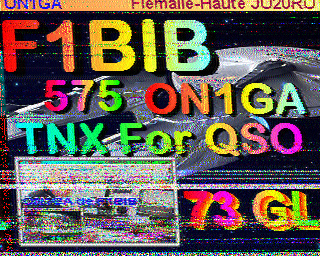
\includegraphics[width=0.85\textwidth]{foto/84}
    \caption{\scriptsize Bestätigung einer SSTV Verbindung an F1BIB von ON1GA mit dem RST 575 und zusätzlich dem ursprünglich empfangenen Bild}
    \label{e_digimode_ssb_sstv}
\end{figure}

   \end{column}
\end{columns}

\end{frame}

\begin{frame}
\frametitle{ATV}
\begin{itemize}
  \item \emph{Amateur Television} ist die Übertragung von Bewegtbildern
  \item Benötigt mehrere MHz Bandbreite (\qty{6}{\mega\hertz} und mehr)
  \item Deshalb nur ab \qty{70}{\centi\metre} Band aufwärts nutzbar
  \end{itemize}
\end{frame}

\begin{frame}
\only<1>{
\begin{QQuestion}{EE415}{Welcher Unterschied zwischen ATV und SSTV ist richtig?}{SSTV wird nur auf Kurzwelle, ATV auf UKW verwendet.}
{SSTV überträgt Standbilder, ATV bewegte Bilder.}
{SSTV belegt eine größere Bandbreite als ATV.}
{SSTV ist schwarzweiß, ATV in Farbe.}
\end{QQuestion}

}
\only<2>{
\begin{QQuestion}{EE415}{Welcher Unterschied zwischen ATV und SSTV ist richtig?}{SSTV wird nur auf Kurzwelle, ATV auf UKW verwendet.}
{\textbf{\textcolor{DARCgreen}{SSTV überträgt Standbilder, ATV bewegte Bilder.}}}
{SSTV belegt eine größere Bandbreite als ATV.}
{SSTV ist schwarzweiß, ATV in Farbe.}
\end{QQuestion}

}
\end{frame}%ENDCONTENT


\section{9600-Port}
\label{section:9600_port}
\begin{frame}%STARTCONTENT
\begin{itemize}
  \item Zur Umgehung von Filtern bieten manche FM-Funkgeräte einen separaten Port für Digimodes
  \item Dieser ist oft mit \emph{DATA} oder \emph{9600} beschriftet
  \item 9600 entsprechend der Datenrate in Baud, die damit übertragen werden kann
  \item Daran wird direkt das TNC (Terminal Node Controller) vom Computer angeschlossen
  \item Heute oft direkt als USB-Anschluss ausgeführt
  \end{itemize}
\end{frame}

\begin{frame}
\begin{columns}
    \begin{column}{0.48\textwidth}
    \begin{itemize}
  \item Sowohl Senden als auch Empfang findet ohne NF-Filter und NF-Endstufe statt
  \item Es wird direkt der FM-Modulator oder FM-Demodulator angesprochen
  \item Signale werden nicht verzerrt
  \end{itemize}

    \end{column}
   \begin{column}{0.48\textwidth}
       
\begin{figure}
    \DARCimage{0.85\linewidth}{354include}
    \caption{\scriptsize FM-Sender mit Zuführung des 9600-Baud-Datensignals an Punkt 2}
    \label{e_9600_port_fm_sender}
\end{figure}


\begin{figure}
    \DARCimage{0.85\linewidth}{355include}
    \caption{\scriptsize FM-Empfänger mit Abgreifen des 9600-Baud-Datensignals an Punkt 4}
    \label{e_9600_port_fm_empfaenger}
\end{figure}


   \end{column}
\end{columns}

\end{frame}

\begin{frame}
\begin{columns}
    \begin{column}{0.48\textwidth}
    \begin{itemize}
  \item Wurde früher für Packet Radio verwendet
  \item Heute für moderne und freie Modi wie M17
  \end{itemize}

    \end{column}
   \begin{column}{0.48\textwidth}
       
\begin{figure}
    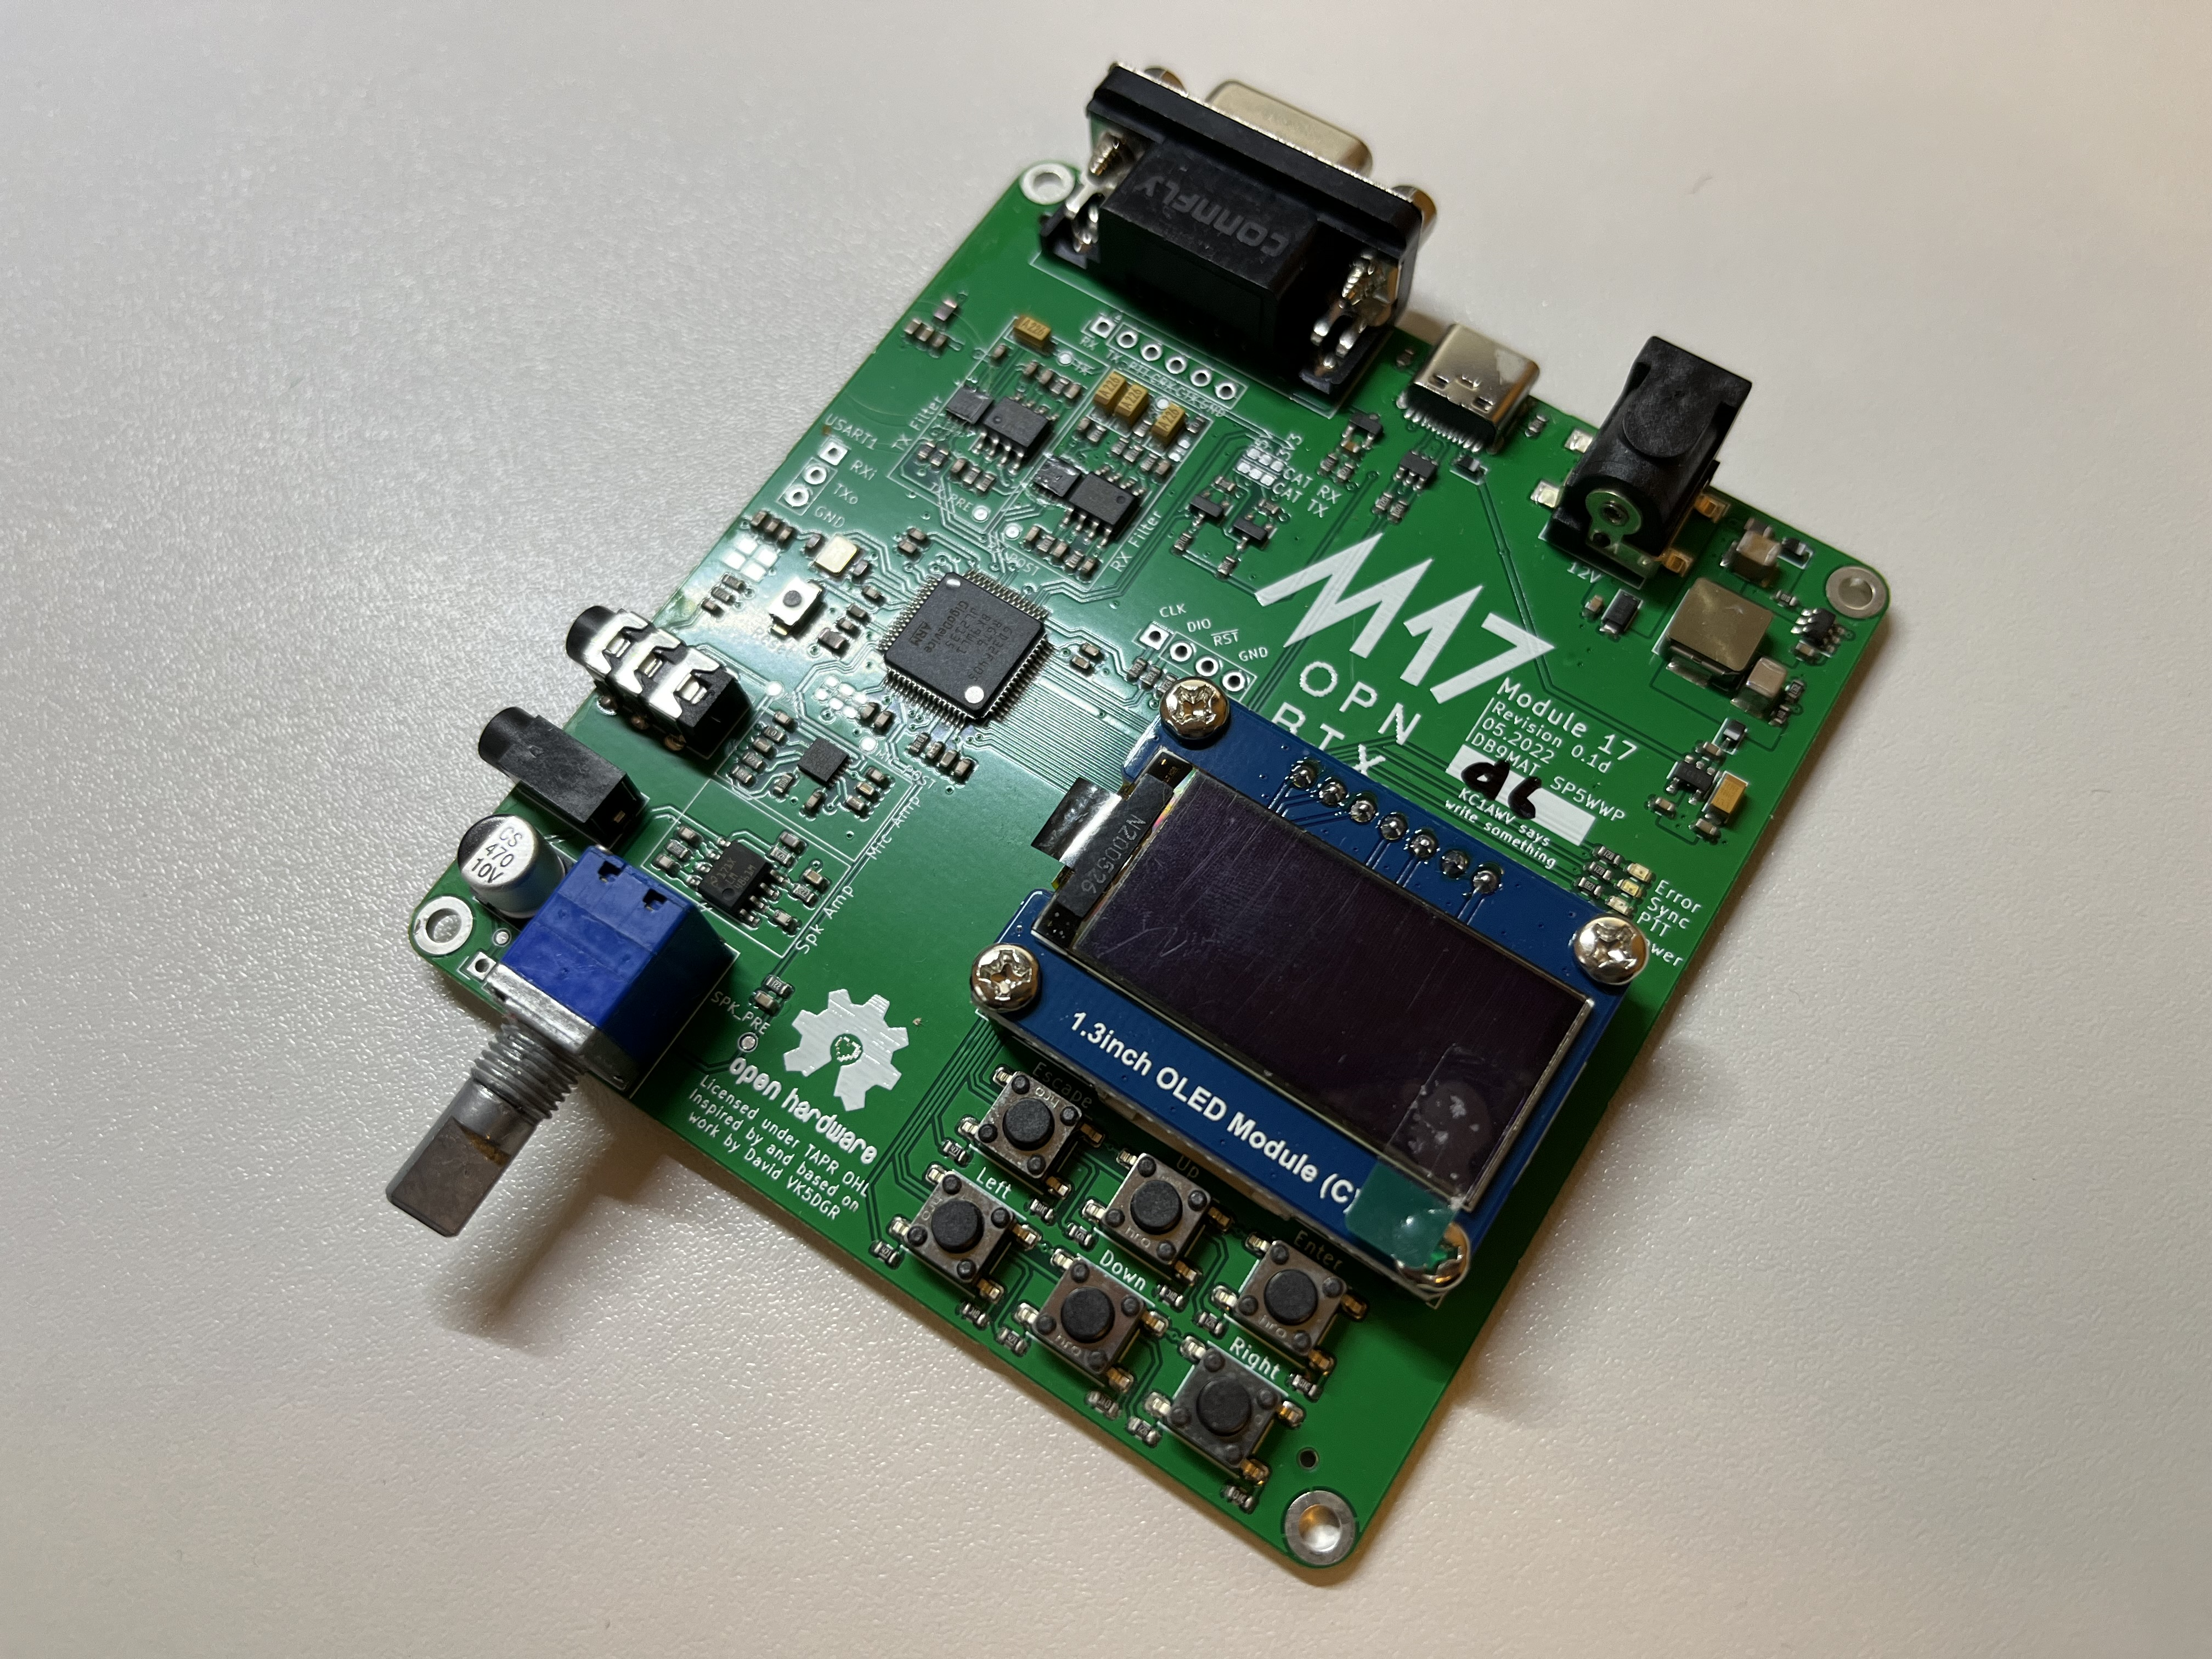
\includegraphics[width=0.85\textwidth]{foto/185}
    \caption{\scriptsize Module M17 ein TNC für das M17 Übertragungsverfahren}
    \label{m17_tnc}
\end{figure}

   \end{column}
\end{columns}

\end{frame}

\begin{frame}
\only<1>{
\begin{PQuestion}{EF309}{Welcher der eingezeichneten Punkte in einem FM-Sender ist für die Zuführung eines 9600-Baud-Datensignals am besten geeignet?}{Punkt 2}
{Punkt 1}
{Punkt 3}
{Punkt 4}
{\DARCimage{1.0\linewidth}{354include}}\end{PQuestion}

}
\only<2>{
\begin{PQuestion}{EF309}{Welcher der eingezeichneten Punkte in einem FM-Sender ist für die Zuführung eines 9600-Baud-Datensignals am besten geeignet?}{\textbf{\textcolor{DARCgreen}{Punkt 2}}}
{Punkt 1}
{Punkt 3}
{Punkt 4}
{\DARCimage{1.0\linewidth}{354include}}\end{PQuestion}

}
\end{frame}

\begin{frame}
\only<1>{
\begin{PQuestion}{EF219}{Manche FM-Transceiver verfügen über einen analogen Datenanschluss (z.~B. mit DATA beschriftet oder als 9600-Port bezeichnet). Welcher Punkt im dargestellten Empfangszweig wird über diesen Anschluss üblicherweise herausgeführt?}{Punkt 1}
{Punkt 4}
{Punkt 2}
{Punkt 3}
{\DARCimage{1.0\linewidth}{355include}}\end{PQuestion}

}
\only<2>{
\begin{PQuestion}{EF219}{Manche FM-Transceiver verfügen über einen analogen Datenanschluss (z.~B. mit DATA beschriftet oder als 9600-Port bezeichnet). Welcher Punkt im dargestellten Empfangszweig wird über diesen Anschluss üblicherweise herausgeführt?}{Punkt 1}
{\textbf{\textcolor{DARCgreen}{Punkt 4}}}
{Punkt 2}
{Punkt 3}
{\DARCimage{1.0\linewidth}{355include}}\end{PQuestion}

}
\end{frame}%ENDCONTENT


\section{Übersteuerung}
\label{section:digimod_uebersteuerung}
\begin{frame}%STARTCONTENT

\begin{columns}
    \begin{column}{0.48\textwidth}
    \begin{itemize}
  \item Zu starkes Audiosignal am Eingang eines Senders $\rightarrow$ Oberschwingungen
  \item Links ist in Gelb das erwünschte Signal
  \item Rechts davon die unerwünschten Oberschwingungen
  \end{itemize}

    \end{column}
   \begin{column}{0.48\textwidth}
       
\begin{figure}
    \DARCimage{0.85\linewidth}{720include}
    \caption{\scriptsize Ein übersteuertes FT8-Signal, ganz links das erwünschte, rechts davon die unerwünschten Oberschwingungen}
    \label{uebersteuerung_ft8}
\end{figure}


   \end{column}
\end{columns}

\end{frame}

\begin{frame}\begin{itemize}
  \item Zu Verzerrungen durch Übersteuerung kann es auch im Sendeverstärker kommen
  \item Um das zu verhindern, verfügen viele Funkgeräte über eine automatische Pegelregelung (englisch: Automatic Level Control, ALC) $\rightarrow$ regelt Verstärkung automatisch runter
  \item Bei digitalen Übertragungsverfahren kann die ALC jedoch Problemen führen
  \item Das Signal könnte je nach Lautstärke oder Frequenz die ALC zu verschiedenen Zeitpunkten unterschiedlich stark auslösen $\rightarrow$ Amplitude wird unerwünscht verändert
  \end{itemize}

\end{frame}

\begin{frame}\begin{itemize}
  \item ALC-Probleme hängen von verschiedenen Faktoren ab
  \item Übertragungsverfahren
  \item Umsetzung der ALC im Transceiver (Reaktions- und Haltezeit)
  \item Anzeige der ALC im Transceiver
  \item $\rightarrow$ greift die ALC nicht ein, erzeugt sie keine Probleme
  \end{itemize}
\end{frame}

\begin{frame}
\only<1>{
\begin{QQuestion}{EJ218}{Wie sollte bei digitalen Übertragungsverfahren (z. B. FT8, JS8, PSK31) der NF-Pegel am Eingang eines Funkgerätes mit automatischer Pegelregelung (ALC) im SSB-Betrieb eingestellt sein, um Störungen zu vermeiden?}{\qty{18}{\decibel} höher als die Lautstärke, bei der die automatische Pegelregelung (ALC) eingreift.}
{So niedrig, dass die automatische Pegelregelung (ALC) nicht eingreift.}
{Alle Bedienelemente sind auf das Maximum einzustellen.}
{Die NF-Lautstärke muss $-\infty$~dB (also Null) betragen.}
\end{QQuestion}

}
\only<2>{
\begin{QQuestion}{EJ218}{Wie sollte bei digitalen Übertragungsverfahren (z. B. FT8, JS8, PSK31) der NF-Pegel am Eingang eines Funkgerätes mit automatischer Pegelregelung (ALC) im SSB-Betrieb eingestellt sein, um Störungen zu vermeiden?}{\qty{18}{\decibel} höher als die Lautstärke, bei der die automatische Pegelregelung (ALC) eingreift.}
{\textbf{\textcolor{DARCgreen}{So niedrig, dass die automatische Pegelregelung (ALC) nicht eingreift.}}}
{Alle Bedienelemente sind auf das Maximum einzustellen.}
{Die NF-Lautstärke muss $-\infty$~dB (also Null) betragen.}
\end{QQuestion}

}
\end{frame}

\begin{frame}
\only<1>{
\begin{QQuestion}{EJ217}{Was kann auftreten, wenn bei digitalen Übertragungsverfahren (z. B. RTTY, FT8, Olivia) die automatische Pegelregelung (ALC) eines Funkgerätes im SSB-Betrieb eingreift?}{Störungen von Stationen auf anderen Frequenzbändern}
{Störungen von Computern oder anderen digitalen Geräten}
{Störungen von Übertragungen auf Nachbarfrequenzen}
{Störungen von nachfolgenden Sendungen auf derselben Frequenz}
\end{QQuestion}

}
\only<2>{
\begin{QQuestion}{EJ217}{Was kann auftreten, wenn bei digitalen Übertragungsverfahren (z. B. RTTY, FT8, Olivia) die automatische Pegelregelung (ALC) eines Funkgerätes im SSB-Betrieb eingreift?}{Störungen von Stationen auf anderen Frequenzbändern}
{Störungen von Computern oder anderen digitalen Geräten}
{\textbf{\textcolor{DARCgreen}{Störungen von Übertragungen auf Nachbarfrequenzen}}}
{Störungen von nachfolgenden Sendungen auf derselben Frequenz}
\end{QQuestion}

}
\end{frame}

\begin{frame}
\only<1>{
\begin{QQuestion}{EJ219}{Was ist zu tun, wenn es bei digitalen Übertragungsverfahren zu Störungen kommt, weil die automatische Pegelregelung (ALC) eines Funkgerätes im SSB-Betrieb eingreift?}{Die Sendeleistung sollte erhöht werden.}
{Der NF-Pegel am Eingang des Funkgerätes sollte reduziert werden.}
{Das Oberwellenfilter sollte abgeschaltet werden.}
{Es sollte mit der RIT gegengesteuert werden.}
\end{QQuestion}

}
\only<2>{
\begin{QQuestion}{EJ219}{Was ist zu tun, wenn es bei digitalen Übertragungsverfahren zu Störungen kommt, weil die automatische Pegelregelung (ALC) eines Funkgerätes im SSB-Betrieb eingreift?}{Die Sendeleistung sollte erhöht werden.}
{\textbf{\textcolor{DARCgreen}{Der NF-Pegel am Eingang des Funkgerätes sollte reduziert werden.}}}
{Das Oberwellenfilter sollte abgeschaltet werden.}
{Es sollte mit der RIT gegengesteuert werden.}
\end{QQuestion}

}
\end{frame}%ENDCONTENT


\section{Automatische Empfangsberichte}
\label{section:automatische_empfangsberichte}
\begin{frame}%STARTCONTENT
\begin{itemize}
  \item Mittels Digimodes empfangene Rufzeichen können an Plattformen geschickt werden
  \item Diese lassen sich auf einer Karte mit empfangenen Band darstellen
  \item Zum Testen der eigenen Ausbreitungsbedingungen
  \end{itemize}

\end{frame}

\begin{frame}
\frametitle{WSPR}
\begin{itemize}
  \item \emph{Weak Signal Progagation Reporter Network}
  \item QRP-Digimode, der rein zum Testen der eigenen Ausbreitungsbedingungen entwickelt wurde
  \item Es ist kein 2-Wege-QSO möglich
  \item Sehr langsame Übertragung mit hoher Fehlerkorrektur
  \item 1 Minute Senden, mehrere Minuten empfangen
  \item Ergebnisse werden an Server geschickt und lassen sich auf WSPRnet (\textcolor{DARCblue}{\faLink~\href{https://www.wsprnet.org/drupal/wsprnet/map}{www.wsprnet.org/drupal/wsprnet/map}}) darstellen
  \end{itemize}
\end{frame}

\begin{frame}
\only<1>{
\begin{QQuestion}{EE405}{Wie können Sie automatische Empfangsberichte zu Aussendungen erhalten, z.~B. um die Reichweite ihrer Sendeanlage zu testen?}{Durch Aussendung einer Nachricht mittels geeignetem digitalen Verfahren (z.~B. CW oder WSPR) und Suche nach Ihrem Rufzeichen auf passenden Internetplattformen}
{Durch Aussendung einer Nachricht mittels geeignetem digitalen Verfahren (z.~B. CW oder WSPR) unter Angabe Ihrer E-Mail-Adresse und der Anzahl der maximal gewünschten Empfangsberichte}
{Durch Aussendung Ihres Rufzeichens mittels Telegrafie (5~WPM) mit dem Zusatz \glqq AUTO RSVP\grqq{} (vom französischen \glqq répondez s'il vous pla\^it\grqq{}) und Abhören der \qty{10}{\kHz} höher gelegenen Frequenz}
{Durch Aussendung Ihres Rufzeichens mittels Telegrafie (12~WPM) mit dem Zusatz \glqq R\grqq{} (für Report) und Abhören der \qty{10}{\kHz} tiefer gelegenen Frequenz}
\end{QQuestion}

}
\only<2>{
\begin{QQuestion}{EE405}{Wie können Sie automatische Empfangsberichte zu Aussendungen erhalten, z.~B. um die Reichweite ihrer Sendeanlage zu testen?}{\textbf{\textcolor{DARCgreen}{Durch Aussendung einer Nachricht mittels geeignetem digitalen Verfahren (z.~B. CW oder WSPR) und Suche nach Ihrem Rufzeichen auf passenden Internetplattformen}}}
{Durch Aussendung einer Nachricht mittels geeignetem digitalen Verfahren (z.~B. CW oder WSPR) unter Angabe Ihrer E-Mail-Adresse und der Anzahl der maximal gewünschten Empfangsberichte}
{Durch Aussendung Ihres Rufzeichens mittels Telegrafie (5~WPM) mit dem Zusatz \glqq AUTO RSVP\grqq{} (vom französischen \glqq répondez s'il vous pla\^it\grqq{}) und Abhören der \qty{10}{\kHz} höher gelegenen Frequenz}
{Durch Aussendung Ihres Rufzeichens mittels Telegrafie (12~WPM) mit dem Zusatz \glqq R\grqq{} (für Report) und Abhören der \qty{10}{\kHz} tiefer gelegenen Frequenz}
\end{QQuestion}

}
\end{frame}%ENDCONTENT


\section{Digital Voice (DV)}
\label{section:digital_voice}
\begin{frame}%STARTCONTENT
\begin{itemize}
  \item Auch Sprache kann digital übertragen werden
  \item z.\,B. mit den Übertragungsverfahren DMR, D-Star, C4FM und M17
  \item Sprachsignale werden vor der Übertragung in einen Datenstrom umgewandelt
  \end{itemize}
\end{frame}

\begin{frame}
\frametitle{TDMA}
Time Division Multiple Access -- Zeitmultiplexverfahren
\begin{columns}
    \begin{column}{0.48\textwidth}
    \begin{itemize}
  \item Übertragung mehrerer Datenströme in schnell abwechselnder Folge
  \item Zwei oder mehr Sprachverbindungen nutzen quasi gleichzeitig dieselbe Frequenz
  \end{itemize}

    \end{column}
   \begin{column}{0.48\textwidth}
       
\begin{figure}
    \DARCimage{0.85\linewidth}{474include}
    \caption{\scriptsize TDMA mit drei Verbindungen auf einer Frequenz}
    \label{n_digital_voice_tdma}
\end{figure}


   \end{column}
\end{columns}

\end{frame}

\begin{frame}
\frametitle{Einstellungen}
Es sind für digitale Sprache oft mehr Einstellungen zu berücksichtigen als zum Beispiel bei einer FM-Verbindung. Zum Beispiel:

\begin{itemize}
  \item Sprechgruppe (Talkgroup)
  \item Raum oder Reflektor zum Zusammenschalten von Relaisfunkstellen
  \item TDMA-Zeitschlitz
  \item Color-Code
  \end{itemize}
\end{frame}

\begin{frame} 
\only<1>{
\begin{QQuestion}{NE404}{Welche Übertragungsverfahren für digitalen Sprechfunk sind im Amateurfunk gebräuchlich?}{FM-Sprechfunk, RTTY, D-STAR, JS8, Olivia}
{AM-Sprechfunk, FM-Sprechfunk, SSB-Sprechfunk, Olivia, SSTV}
{DMR, D-STAR, C4FM, M17, FreeDV}
{SSB-Sprechfunk, FT8, DMR, PSK31, SSTV}
\end{QQuestion}

}
\only<2>{
\begin{QQuestion}{NE404}{Welche Übertragungsverfahren für digitalen Sprechfunk sind im Amateurfunk gebräuchlich?}{FM-Sprechfunk, RTTY, D-STAR, JS8, Olivia}
{AM-Sprechfunk, FM-Sprechfunk, SSB-Sprechfunk, Olivia, SSTV}
{\textbf{\textcolor{DARCgreen}{DMR, D-STAR, C4FM, M17, FreeDV}}}
{SSB-Sprechfunk, FT8, DMR, PSK31, SSTV}
\end{QQuestion}

}
\end{frame}

\begin{frame} 
\only<1>{
\begin{QQuestion}{NE307}{Welche Übertragungsverfahren werden bei VHF/UHF-Handfunkgeräten üblicherweise verwendet?}{CW-Morsetelegrafie, FT8, D-STAR}
{FM-Sprechfunk, DMR, D-STAR}
{SSB-Sprechfunk, DMR, RTTY}
{AM-Sprechfunk, C4FM, FT8}
\end{QQuestion}

}
\only<2>{
\begin{QQuestion}{NE307}{Welche Übertragungsverfahren werden bei VHF/UHF-Handfunkgeräten üblicherweise verwendet?}{CW-Morsetelegrafie, FT8, D-STAR}
{\textbf{\textcolor{DARCgreen}{FM-Sprechfunk, DMR, D-STAR}}}
{SSB-Sprechfunk, DMR, RTTY}
{AM-Sprechfunk, C4FM, FT8}
\end{QQuestion}

}
\end{frame}

\begin{frame} 
\only<1>{
\begin{QQuestion}{NE403}{Ist es bei bestimmten digitalen Verfahren zur Sprachübertragung (z.~B. DMR oder TETRA) möglich, mehrere Sprechverbindungen gleichzeitig auf derselben Frequenz innerhalb eines Empfangsgebiets abzuwickeln?}{Nein. Sprachübertragungen können nicht in Datenpakete aufgeteilt werden.}
{Ja. Die Sendeleistung wird zur Verbesserung der digitalen Fehlerkorrektur erhöht.}
{Nein. Zeitgleich stattfindende digitale Übertragungen stören sich prinzipbedingt gegenseitig.}
{Ja. Die Sprachdaten werden abwechselnd in periodischen, kurzen Zeitschlitzen übertragen.}
\end{QQuestion}

}
\only<2>{
\begin{QQuestion}{NE403}{Ist es bei bestimmten digitalen Verfahren zur Sprachübertragung (z.~B. DMR oder TETRA) möglich, mehrere Sprechverbindungen gleichzeitig auf derselben Frequenz innerhalb eines Empfangsgebiets abzuwickeln?}{Nein. Sprachübertragungen können nicht in Datenpakete aufgeteilt werden.}
{Ja. Die Sendeleistung wird zur Verbesserung der digitalen Fehlerkorrektur erhöht.}
{Nein. Zeitgleich stattfindende digitale Übertragungen stören sich prinzipbedingt gegenseitig.}
{\textbf{\textcolor{DARCgreen}{Ja. Die Sprachdaten werden abwechselnd in periodischen, kurzen Zeitschlitzen übertragen.}}}
\end{QQuestion}

}
\end{frame}

\begin{frame} 
\only<1>{
\begin{QQuestion}{NE402}{Sie möchten an einer Funkrunde mittels digitaler Sprachübertragung (z.~B. C4FM, DMR oder D-Star) über ein Repeaternetzwerk teilnehmen. Worauf müssen Sie neben der Wahl des Übertragungsverfahrens, der Frequenz und der Modulation achten?}{Alle Stationen müssen sich in Funkreichweite desselben Repeaters befinden.}
{Sie müssen die gleiche Firmwareversion wie das Repeaternetzwerk verwenden.}
{Alle Stationen müssen die gleiche Stationskennung, z.~B. DMR-ID, einstellen.}
{Sie müssen geeignete Parameter, z.~B. Reflektor, Zeitschlitz oder Color-Code, wählen.}
\end{QQuestion}

}
\only<2>{
\begin{QQuestion}{NE402}{Sie möchten an einer Funkrunde mittels digitaler Sprachübertragung (z.~B. C4FM, DMR oder D-Star) über ein Repeaternetzwerk teilnehmen. Worauf müssen Sie neben der Wahl des Übertragungsverfahrens, der Frequenz und der Modulation achten?}{Alle Stationen müssen sich in Funkreichweite desselben Repeaters befinden.}
{Sie müssen die gleiche Firmwareversion wie das Repeaternetzwerk verwenden.}
{Alle Stationen müssen die gleiche Stationskennung, z.~B. DMR-ID, einstellen.}
{\textbf{\textcolor{DARCgreen}{Sie müssen geeignete Parameter, z.~B. Reflektor, Zeitschlitz oder Color-Code, wählen.}}}
\end{QQuestion}

}
\end{frame}%ENDCONTENT


\section{Paketvermittelte Netzwerke}
\label{section:paketvermittelte_netzwerke}
\begin{frame}%STARTCONTENT
\begin{itemize}
  \item Das HAMNET, das Netzwerk nur für Funkamateure, basiert auf dem Internet-Protokoll (IP).
  \item Deswegen kann man das Hamnet mit der gleichen Software, die auch für das Internet verwendet wird, nutzen.
  \item Im einfachsten Fall ist das ein Webbrowser.
  \end{itemize}
\end{frame}

\begin{frame}\begin{itemize}
  \item Das Internet-Protokoll (IP) weist den beteiligten Computern IP-Adressen zu, damit sie sich gegenseitig erreichen können.
  \item IP-Adressen werden als vier Dezimalzahlen mit einem Punkt dazwischen geschrieben. Beispiel: 141.17.5.18
  \item Jede Dezimalzahl hat eine Länge von 8 Bit, deswegen ist die größtmögliche Zahl 255 (binär: 11111111).
  \end{itemize}

\end{frame}

\begin{frame}\begin{itemize}
  \item IP-Adressen sind in einen Netz- und einen Hostanteil aufgeteilt.
  \item Bei allen Computern, die sich im selben Netzwerk befinden, ist der Anfang der IP-Adressen gleich, diesen Anfang nennt man Netzanteil.
  \item Der Netzanteil ist unterschiedlich groß, je nachdem wie viele Computer (Hosts) im Netzwerk verwaltet werden sollen.
  \end{itemize}
\end{frame}

\begin{frame}Beispiele:

\emph{10}.100.234.22 (kleiner Netzanteil, großer Hostanteil)

\emph{192.168.1}.252 (großer Netzanteil, kleiner Hostanteil)

Dieses Prinzip kennt man vom Telefonnetz. Die großen Städte haben kürzere Vorwahlen als kleine Städte.

\end{frame}

\begin{frame}
\begin{figure}
    \DARCimage{0.85\linewidth}{699include}
    \caption{\scriptsize IPv4-Adresse und Netzmaske in Dezimal- und Dualschreibweise}
    \label{netzmaske}
\end{figure}

\begin{itemize}
  \item Eine Subnetzmaske gibt die Aufteilung einer IP-Adresse in Netz- und Hostanteil an, indem sie alle Bits des Netzanteils als 1 darstellt.
  \end{itemize}
\end{frame}

\begin{frame}\begin{itemize}
  \item Es zwei Möglichkeiten dieses niederzuschreiben, Beispiel für einen Netzanteil von 24:
  \item 255.255.255.0, was binär 11111111.11111111.11111111.00000000 ist.
  \item Die Schreibweise mit dem Schrägstrich, zum Beispiel 192.168.111.90/24
  \end{itemize}

\end{frame}

\begin{frame}
\begin{figure}
    \DARCimage{0.85\linewidth}{706include}
    \caption{\scriptsize Ausschnitt aus einer Netzwerk-Infrastruktur}
    \label{netzwerk}
\end{figure}

\begin{itemize}
  \item Netzwerkgeräte können nur innerhalb ihres eigenen lokalen Netzwerks direkt miteinander kommunizieren.
  \end{itemize}
\end{frame}

\begin{frame}
\begin{figure}
    \DARCimage{0.85\linewidth}{706include}
    \caption{\scriptsize Ausschnitt aus einer Netzwerk-Infrastruktur}
    \label{netzwerk}
\end{figure}

\begin{itemize}
  \item Man erkennt sie daran, dass sich aus ihrer eigenen IP-Adresse und Subnetzmaske derselbe Netzanteil ergibt wie beim Partner.
  \end{itemize}
\end{frame}

\begin{frame}
\begin{figure}
    \DARCimage{0.85\linewidth}{706include}
    \caption{\scriptsize Ausschnitt aus einer Netzwerk-Infrastruktur}
    \label{netzwerk}
\end{figure}

\begin{itemize}
  \item In allen anderen Fällen schicken sie die Daten an einen Router. Das ist eine Zwischenstation, die zwei oder mehr Netzwerke miteinander verbindet, um die Datenpakete weiterzuleiten.
  \end{itemize}
\end{frame}

\begin{frame}
\only<1>{
\begin{QQuestion}{EE412}{Wie können Informationen innerhalb eines paketvermittelten Netzes zwischen zwei Stationen ausgetauscht werden, die sich nicht direkt erreichen können?}{Durch wiederholte Aussendung (Paketwiederholung)}
{Durch Weiterleitung über Zwischenstationen (Paketweiterleitung)}
{Durch Entpacken vor der Sendung (Paketdekompression)}
{Durch Zusammenfassung von Übertragungen (Paketdefragmentierung)}
\end{QQuestion}

}
\only<2>{
\begin{QQuestion}{EE412}{Wie können Informationen innerhalb eines paketvermittelten Netzes zwischen zwei Stationen ausgetauscht werden, die sich nicht direkt erreichen können?}{Durch wiederholte Aussendung (Paketwiederholung)}
{\textbf{\textcolor{DARCgreen}{Durch Weiterleitung über Zwischenstationen (Paketweiterleitung)}}}
{Durch Entpacken vor der Sendung (Paketdekompression)}
{Durch Zusammenfassung von Übertragungen (Paketdefragmentierung)}
\end{QQuestion}

}
\end{frame}

\begin{frame}
\only<1>{
\begin{QQuestion}{EE414}{Kann das Internetprotokoll (IP) im Amateurfunk verwendet werden?}{Nein, Internetnutzern würde so Zugang zum Amateurfunkband ermöglicht.}
{Ja, die Kodierung des Amateurfunkrufzeichens erfolgt in der Subnetzmaske.}
{Ja, es ist nicht auf das Internet beschränkt.}
{Nein, die benötigte Bandbreite steht im Amateurfunk nicht zur Verfügung.}
\end{QQuestion}

}
\only<2>{
\begin{QQuestion}{EE414}{Kann das Internetprotokoll (IP) im Amateurfunk verwendet werden?}{Nein, Internetnutzern würde so Zugang zum Amateurfunkband ermöglicht.}
{Ja, die Kodierung des Amateurfunkrufzeichens erfolgt in der Subnetzmaske.}
{\textbf{\textcolor{DARCgreen}{Ja, es ist nicht auf das Internet beschränkt.}}}
{Nein, die benötigte Bandbreite steht im Amateurfunk nicht zur Verfügung.}
\end{QQuestion}

}
\end{frame}

\begin{frame}
\only<1>{
\begin{QQuestion}{EE413}{Was ergibt sich aus der eingestellten IP-Adresse und Subnetzmaske einer Kommunikationsschnittstelle beim Internetprotokoll (IP)?}{Das Standardgateway und die maximale Anzahl der Zwischenstationen (Hops)}
{Die Protokoll- und Portnummer des über die Schnittstelle verwendeten Protokolls}
{Die Gegenstelle und die durch das Teilnetz verwendete Bandbreite}
{Der direkt (d.~h. ohne Router) über die Schnittstelle erreichbare Adressbereich}
\end{QQuestion}

}
\only<2>{
\begin{QQuestion}{EE413}{Was ergibt sich aus der eingestellten IP-Adresse und Subnetzmaske einer Kommunikationsschnittstelle beim Internetprotokoll (IP)?}{Das Standardgateway und die maximale Anzahl der Zwischenstationen (Hops)}
{Die Protokoll- und Portnummer des über die Schnittstelle verwendeten Protokolls}
{Die Gegenstelle und die durch das Teilnetz verwendete Bandbreite}
{\textbf{\textcolor{DARCgreen}{Der direkt (d.~h. ohne Router) über die Schnittstelle erreichbare Adressbereich}}}
\end{QQuestion}

}
\end{frame}%ENDCONTENT


\section{Amplituden- und Frequenzumtastung (ASK, FSK)}
\label{section:ask_fsk_afsk}
\begin{frame}%STARTCONTENT
\begin{itemize}
  \item Genauso wie es verschiedene analoge Modulationsverfahren gibt, gibt es auch verschiedene digitale Modulationsverfahren.
  \item Die grundlegenden Möglichkeiten ein Signal zu modulieren, also auf einen Hochfrequenzträger aufzuprägen, sind dieselben: Veränderung der Amplitude, der Frequenz oder der Phase des Trägers.
  \item Beim unmodulierten Träger hingegen bleiben Amplitude, Frequenz und Phasenlage konstant.
  \end{itemize}
\end{frame}

\begin{frame}\begin{itemize}
  \item Bei der Amplitudenumtastung (Amplitude Shift Keying, ASK) wird im einfachsten Fall zwischen zwei Amplituden gewechselt.
  \end{itemize}
    \pause
    
\begin{figure}
    \DARCimage{0.85\linewidth}{700include}
    \caption{\scriptsize Amplitudenumtastung (Amplitude-shift Keying)}
    \label{ask}
\end{figure}



\end{frame}

\begin{frame}\begin{itemize}
  \item Bei der Frequenzumstastung (Frequency Shift Keying, FSK) wechselt der Sender zwischen bestimmten Frequenzen.
  \end{itemize}
    \pause
    
\begin{figure}
    \DARCimage{0.85\linewidth}{703include}
    \caption{\scriptsize Frequenzumtastung (Frequency-shift Keying)}
    \label{fsk}
\end{figure}



\end{frame}

\begin{frame}\begin{itemize}
  \item Bei der Phasenumtastung (Phase Shift Keying, PSK) wechselt der Sender zwischen bestimmten Phasenlagen.
  \end{itemize}
    \pause
    
\begin{figure}
    \DARCimage{0.85\linewidth}{705include}
    \caption{\scriptsize Phasenumtastung (Phase-shift Keying)}
    \label{psk}
\end{figure}



\end{frame}

\begin{frame}
\only<1>{
\begin{question2x2}{EE406}{Welches der folgenden Diagramme zeigt einen erkennbar durch Amplitudenumtastung (ASK) modulierten Träger?}{\DARCimage{1.0\linewidth}{357include}}
{\DARCimage{1.0\linewidth}{356include}}
{\DARCimage{1.0\linewidth}{358include}}
{\DARCimage{1.0\linewidth}{359include}}
\end{question2x2}

}
\only<2>{
\begin{question2x2}{EE406}{Welches der folgenden Diagramme zeigt einen erkennbar durch Amplitudenumtastung (ASK) modulierten Träger?}{\DARCimage{1.0\linewidth}{357include}}
{\DARCimage{1.0\linewidth}{356include}}
{\textbf{\textcolor{DARCgreen}{\DARCimage{1.0\linewidth}{358include}}}}
{\DARCimage{1.0\linewidth}{359include}}
\end{question2x2}

}
\end{frame}

\begin{frame}
\only<1>{
\begin{question2x2}{EE407}{Welches der folgenden Diagramme zeigt einen erkennbar durch Frequenzumtastung (FSK) modulierten Träger?}{\DARCimage{1.0\linewidth}{357include}}
{\DARCimage{1.0\linewidth}{356include}}
{\DARCimage{1.0\linewidth}{358include}}
{\DARCimage{1.0\linewidth}{359include}}
\end{question2x2}

}
\only<2>{
\begin{question2x2}{EE407}{Welches der folgenden Diagramme zeigt einen erkennbar durch Frequenzumtastung (FSK) modulierten Träger?}{\textbf{\textcolor{DARCgreen}{\DARCimage{1.0\linewidth}{357include}}}}
{\DARCimage{1.0\linewidth}{356include}}
{\DARCimage{1.0\linewidth}{358include}}
{\DARCimage{1.0\linewidth}{359include}}
\end{question2x2}

}
\end{frame}

\begin{frame}
\only<1>{
\begin{question2x2}{AE401}{Welches der folgenden Diagramme zeigt einen erkennbar durch Phasenumtastung (PSK) modulierten Träger?}{\DARCimage{1.0\linewidth}{357include}}
{\DARCimage{1.0\linewidth}{356include}}
{\DARCimage{1.0\linewidth}{359include}}
{\DARCimage{1.0\linewidth}{358include}}
\end{question2x2}

}
\only<2>{
\begin{question2x2}{AE401}{Welches der folgenden Diagramme zeigt einen erkennbar durch Phasenumtastung (PSK) modulierten Träger?}{\DARCimage{1.0\linewidth}{357include}}
{\DARCimage{1.0\linewidth}{356include}}
{\textbf{\textcolor{DARCgreen}{\DARCimage{1.0\linewidth}{359include}}}}
{\DARCimage{1.0\linewidth}{358include}}
\end{question2x2}

}
\end{frame}

\begin{frame}
\only<1>{
\begin{question2x2}{EE101}{Welches der folgenden Diagramme zeigt einen unmodulierten Träger?}{\DARCimage{1.0\linewidth}{356include}}
{\DARCimage{1.0\linewidth}{357include}}
{\DARCimage{1.0\linewidth}{359include}}
{\DARCimage{1.0\linewidth}{358include}}
\end{question2x2}

}
\only<2>{
\begin{question2x2}{EE101}{Welches der folgenden Diagramme zeigt einen unmodulierten Träger?}{\textbf{\textcolor{DARCgreen}{\DARCimage{1.0\linewidth}{356include}}}}
{\DARCimage{1.0\linewidth}{357include}}
{\DARCimage{1.0\linewidth}{359include}}
{\DARCimage{1.0\linewidth}{358include}}
\end{question2x2}

}
\end{frame}%ENDCONTENT


\section{Phasenumtastung (PSK)}
\label{section:psk}
\begin{frame}%STARTCONTENT

\only<1>{
\begin{question2x2}{AE401}{Welches der folgenden Diagramme zeigt einen erkennbar durch Phasenumtastung (PSK) modulierten Träger?}{\DARCimage{1.0\linewidth}{357include}}
{\DARCimage{1.0\linewidth}{356include}}
{\DARCimage{1.0\linewidth}{359include}}
{\DARCimage{1.0\linewidth}{358include}}
\end{question2x2}

}
\only<2>{
\begin{question2x2}{AE401}{Welches der folgenden Diagramme zeigt einen erkennbar durch Phasenumtastung (PSK) modulierten Träger?}{\DARCimage{1.0\linewidth}{357include}}
{\DARCimage{1.0\linewidth}{356include}}
{\textbf{\textcolor{DARCgreen}{\DARCimage{1.0\linewidth}{359include}}}}
{\DARCimage{1.0\linewidth}{358include}}
\end{question2x2}

}
\end{frame}%ENDCONTENT


\section{Symbolumschaltung und Bandbreite}
\label{section:symbolumschaltung_bandbreite}
\begin{frame}%STARTCONTENT
\begin{itemize}
  \item Als Symbol werden in der Digitaltechnik die verschiedenen Zeicheneinheiten zur Übertragung des Informationsgehaltes bezeichnet.
  \item Die Anzahl der pro Zeitspanne übertragenen Symbole ist die Symbolrate und wird in der Einheit Baud ausgedrückt.
  \item Bei jeder Umschaltung zwischen zwei Symbolen wird die Amplitude, Frequenz oder Phase eines Trägers geändert.
  \item Je schneller Amplitude, Frequenz oder Phase verändert werden, umso breitbandiger wird das erzeugte Signal.
  \end{itemize}
\end{frame}

\begin{frame}
\only<1>{
\begin{QQuestion}{AE415}{Welche Auswirkung hat eine Erhöhung der Umschaltgeschwindigkeit zwischen verschiedenen Symbolen bei digitalen Übertragungsverfahren auf die benötigte Bandbreite? Die Bandbreite~...}{bleibt gleich.}
{sinkt.}
{steigt.}
{steigt im oberen und sinkt im unteren Seitenband.}
\end{QQuestion}

}
\only<2>{
\begin{QQuestion}{AE415}{Welche Auswirkung hat eine Erhöhung der Umschaltgeschwindigkeit zwischen verschiedenen Symbolen bei digitalen Übertragungsverfahren auf die benötigte Bandbreite? Die Bandbreite~...}{bleibt gleich.}
{sinkt.}
{\textbf{\textcolor{DARCgreen}{steigt.}}}
{steigt im oberen und sinkt im unteren Seitenband.}
\end{QQuestion}

}
\end{frame}

\begin{frame}
\only<1>{
\begin{question2x2}{AE214}{Welches dieser amplitudenmodulierten Signale belegt die geringste Bandbreite?}{\DARCimage{1.0\linewidth}{599include}}
{\DARCimage{1.0\linewidth}{598include}}
{\DARCimage{1.0\linewidth}{597include}}
{\DARCimage{1.0\linewidth}{601include}}
\end{question2x2}

}
\only<2>{
\begin{question2x2}{AE214}{Welches dieser amplitudenmodulierten Signale belegt die geringste Bandbreite?}{\DARCimage{1.0\linewidth}{599include}}
{\DARCimage{1.0\linewidth}{598include}}
{\textbf{\textcolor{DARCgreen}{\DARCimage{1.0\linewidth}{597include}}}}
{\DARCimage{1.0\linewidth}{601include}}
\end{question2x2}

}
\end{frame}

\begin{frame}\begin{itemize}
  \item Von der Morsetelegrafie kennen wir bereits Tastklicks, die breitbandige Störungen darstellen.
  \item Sie entstehen, wenn beim Drücken bzw. Loslassen der Morsetaste der Träger plötzlich ein- bzw. ausgeschaltet wird.
  \end{itemize}
\end{frame}

\begin{frame}
\only<1>{
\begin{question2x2}{AJ221}{In den nachfolgenden Bildern sind mögliche Signalverläufe des Senderausgangssignals bei der CW-Tastung dargestellt. Welcher Signalverlauf führt zu den geringsten Störungen?}{\DARCimage{1.0\linewidth}{21include}}
{\DARCimage{1.0\linewidth}{20include}}
{\DARCimage{1.0\linewidth}{19include}}
{\DARCimage{1.0\linewidth}{22include}}
\end{question2x2}

}
\only<2>{
\begin{question2x2}{AJ221}{In den nachfolgenden Bildern sind mögliche Signalverläufe des Senderausgangssignals bei der CW-Tastung dargestellt. Welcher Signalverlauf führt zu den geringsten Störungen?}{\DARCimage{1.0\linewidth}{21include}}
{\DARCimage{1.0\linewidth}{20include}}
{\textbf{\textcolor{DARCgreen}{\DARCimage{1.0\linewidth}{19include}}}}
{\DARCimage{1.0\linewidth}{22include}}
\end{question2x2}

}
\end{frame}

\begin{frame}
\only<1>{
\begin{PQuestion}{AJ220}{Diese Modulationshüllkurve eines CW-Senders sollte vermieden werden, da~...}{wahrscheinlich Tastklicks erzeugt werden.}
{während der Aussetzer Probleme im Leistungsverstärker entstehen könnten.}
{die ausgesendeten Signale schwierig zu lesen sind.}
{die Stromversorgung überlastet wird.}
{\DARCimage{1.0\linewidth}{12include}}\end{PQuestion}

}
\only<2>{
\begin{PQuestion}{AJ220}{Diese Modulationshüllkurve eines CW-Senders sollte vermieden werden, da~...}{\textbf{\textcolor{DARCgreen}{wahrscheinlich Tastklicks erzeugt werden.}}}
{während der Aussetzer Probleme im Leistungsverstärker entstehen könnten.}
{die ausgesendeten Signale schwierig zu lesen sind.}
{die Stromversorgung überlastet wird.}
{\DARCimage{1.0\linewidth}{12include}}\end{PQuestion}

}
\end{frame}%ENDCONTENT


\section{Mehrwertige Verfahren}
\label{section:mehrwertige_verfahren}
\begin{frame}%STARTCONTENT
\begin{itemize}
  \item Viele digitale Modulationsverfahren verwenden mehr als zwei Symbole.
  \item So funktioniert zum Beispiel die 4-Fach-Amplitudenumtastung (4ASK) mit vier unterschiedlichen Amplituden, 25 %, 50 %, 75 %, 100 % des Maximums.
  \item So lassen sich zwei Bits zu einem Symbol zusammenfassen und gleichzeitig übertragen.
  \end{itemize}

\begin{figure}
    \DARCimage{0.85\linewidth}{701include}
    \caption{\scriptsize Quaternäre Amplitudenumtastung (Quaternary Amplitude-shift Keying)}
    \label{4ask}
\end{figure}

\end{frame}

\begin{frame}\begin{itemize}
  \item Dieses Prinzip lässt sich auf die Frequenz- und Phasenumtastung übertragen.
  \item Eine einfache Phasenumtastung (Binary Phase-Shift Keying, BPSK) verwendet nur zwei verschiedene Phasenlagen und kann daher nur ein Bit gleichzeitig senden.
  \item Die Quadraturphasenumtastung (Quadrature Phase-Shift Keying, QPSK) hingegen nutzt vier verschiedene Phasenlagen (0 °, 90 °, 180 ° und 270 °) und überträgt somit zwei Bits in jedem Schritt.
  \end{itemize}
\end{frame}

\begin{frame}
\only<1>{
\begin{QQuestion}{AE402}{Was unterscheidet BPSK- und QPSK-Modulation?}{Mit BPSK wird ein Bit pro Symbol übertragen, mit QPSK zwei Bit pro Symbol.}
{Mit QPSK wird ein Bit pro Symbol übertragen, mit BPSK zwei Bit pro Symbol.}
{Bei BPSK werden der I- und der Q-Anteil eines I/Q-Signals vertauscht, bei QPSK nicht.}
{Bei QPSK werden der I- und der Q-Anteil eines I/Q-Signals vertauscht, bei BPSK nicht.}
\end{QQuestion}

}
\only<2>{
\begin{QQuestion}{AE402}{Was unterscheidet BPSK- und QPSK-Modulation?}{\textbf{\textcolor{DARCgreen}{Mit BPSK wird ein Bit pro Symbol übertragen, mit QPSK zwei Bit pro Symbol.}}}
{Mit QPSK wird ein Bit pro Symbol übertragen, mit BPSK zwei Bit pro Symbol.}
{Bei BPSK werden der I- und der Q-Anteil eines I/Q-Signals vertauscht, bei QPSK nicht.}
{Bei QPSK werden der I- und der Q-Anteil eines I/Q-Signals vertauscht, bei BPSK nicht.}
\end{QQuestion}

}
\end{frame}

\begin{frame}\begin{itemize}
  \item Da bei Verfahren wie QPSK mehr als ein Bit pro Symbol übertragen wird, müssen wir mit den Einheiten aufpassen.
  \item Werden nur zwei Symbole verwendet und somit jedes Bit einzeln gesendet, entspricht die Symbolrate in Baud der Datenrate in Bit/s.
  \item Werden jedoch mehr Symbole verwendet und somit mehrere Bits gleichzeitig übertragen, ist die Datenrate höher als die Symbolrate.
  \end{itemize}
\end{frame}

\begin{frame}\begin{itemize}
  \item Die Formel $C = R_{ s } \cdot n$ stellt den Zusammenhang dar:
  \end{itemize}
C → Datenübertragungsrate in Bit/s

$R_{ s }$ → Symbolrate in Baud

n → Symbolgröße in Bit/Symbol

\end{frame}

\begin{frame}
\only<1>{
\begin{QQuestion}{AA104}{Welche Einheit wird üblicherweise für die Symbolrate verwendet?}{Bit pro Sekunde (Bit/s)}
{Baud (Bd)}
{Hertz (Hz)}
{Dezibel (dB)}
\end{QQuestion}

}
\only<2>{
\begin{QQuestion}{AA104}{Welche Einheit wird üblicherweise für die Symbolrate verwendet?}{Bit pro Sekunde (Bit/s)}
{\textbf{\textcolor{DARCgreen}{Baud (Bd)}}}
{Hertz (Hz)}
{Dezibel (dB)}
\end{QQuestion}

}
\end{frame}

\begin{frame}Beispiele:

\emph{RTTY}: Umschaltung zwischen zwei Symbolfrequenzen, so dass pro Symbol ein Bit (0 oder 1) übertragen werden kann.

→ Datenrate = Symbolrate

\emph{FT4}: Umschaltung zwischen vier Symbolfrequenzen, so dass pro Symbol zwei Bit (00, 01, 10 oder 11) übertragen werden können.

→ Datenrate = 2 $\cdot$ Symbolrate

\end{frame}

\begin{frame}
\only<1>{
\begin{QQuestion}{AE405}{Bei einem digitalen Übertragungsverfahren (z.~B. RTTY) wird die Frequenz eines Senders zwischen zwei Symbolfrequenzen (z.~B. \qty{14072,43}{\kHz} und \qty{14072,60}{\kHz}) umgetastet, so dass pro Symbol ein Bit (0 oder 1) übertragen werden kann. Die Symbolrate beträgt \qty{45,45}{\baud}. Welcher Datenrate entspricht das?}{\qty[per-mode=symbol]{22,725}{\bit\per\s}}
{\qty[per-mode=symbol]{90,9}{\bit\per\s}}
{\qty[per-mode=symbol]{45,45}{\bit\per\s}}
{\qty[per-mode=symbol]{181,8}{\bit\per\s}}
\end{QQuestion}

}
\only<2>{
\begin{QQuestion}{AE405}{Bei einem digitalen Übertragungsverfahren (z.~B. RTTY) wird die Frequenz eines Senders zwischen zwei Symbolfrequenzen (z.~B. \qty{14072,43}{\kHz} und \qty{14072,60}{\kHz}) umgetastet, so dass pro Symbol ein Bit (0 oder 1) übertragen werden kann. Die Symbolrate beträgt \qty{45,45}{\baud}. Welcher Datenrate entspricht das?}{\qty[per-mode=symbol]{22,725}{\bit\per\s}}
{\qty[per-mode=symbol]{90,9}{\bit\per\s}}
{\textbf{\textcolor{DARCgreen}{\qty[per-mode=symbol]{45,45}{\bit\per\s}}}}
{\qty[per-mode=symbol]{181,8}{\bit\per\s}}
\end{QQuestion}

}
\end{frame}

\begin{frame}
\frametitle{Lösungsweg}
\begin{itemize}
  \item gegeben: $R_S = 45,45Bd$
  \item gegeben: $n=1\frac{Bit}{Symbol}$
  \item gesucht: $C$
  \end{itemize}
    \pause
    $C = R_S \cdot n = 45,45Bd \cdot 1 = 45,45\frac{Bit}{s}$



\end{frame}

\begin{frame}
\only<1>{
\begin{QQuestion}{AE406}{Bei einem digitalen Übertragungsverfahren (z.~B. FT4) wird die Frequenz eines Senders zwischen vier Symbolfrequenzen (z.~B. \qty{14081,20}{\kHz}, \qty{14081,40}{\kHz}, \qty{14081,61}{\kHz} und \qty{14081,83}{\kHz}) umgetastet, so dass pro Symbol zwei Bit (00, 01, 10 oder 11) übertragen werden können. Die Symbolrate beträgt \qty{23,4}{\baud}. Welcher Datenrate entspricht das?}{\qty[per-mode=symbol]{93,6}{\bit\per\s}}
{\qty[per-mode=symbol]{11,7}{\bit\per\s}}
{\qty[per-mode=symbol]{23,4}{\bit\per\s}}
{\qty[per-mode=symbol]{46,8}{\bit\per\s}}
\end{QQuestion}

}
\only<2>{
\begin{QQuestion}{AE406}{Bei einem digitalen Übertragungsverfahren (z.~B. FT4) wird die Frequenz eines Senders zwischen vier Symbolfrequenzen (z.~B. \qty{14081,20}{\kHz}, \qty{14081,40}{\kHz}, \qty{14081,61}{\kHz} und \qty{14081,83}{\kHz}) umgetastet, so dass pro Symbol zwei Bit (00, 01, 10 oder 11) übertragen werden können. Die Symbolrate beträgt \qty{23,4}{\baud}. Welcher Datenrate entspricht das?}{\qty[per-mode=symbol]{93,6}{\bit\per\s}}
{\qty[per-mode=symbol]{11,7}{\bit\per\s}}
{\qty[per-mode=symbol]{23,4}{\bit\per\s}}
{\textbf{\textcolor{DARCgreen}{\qty[per-mode=symbol]{46,8}{\bit\per\s}}}}
\end{QQuestion}

}
\end{frame}

\begin{frame}
\frametitle{Lösungsweg}
\begin{itemize}
  \item gegeben: $R_S = 23,4Bd$
  \item gegeben: $n=2\frac{Bit}{Symbol}$
  \item gesucht: $C$
  \end{itemize}
    \pause
    $C = R_S \cdot n = 23,4 \cdot 2 = 46,8\frac{Bit}{s}$



\end{frame}%ENDCONTENT


\section{Quadraturamplitudenmodulation  (QAM)}
\label{section:qam}
\begin{frame}%STARTCONTENT
\begin{itemize}
  \item Es scheint zunächst nahe zu liegen, die Anzahl der Symbole möglichst groß zu wählen, damit pro Symbol möglichst viele Informationen übertragen werden können.
  \item Doch dann muss ein Empfänger z.B. zwischen vielen unterschiedlichen Amplituden unterscheiden können. Somit wird das Verfahren anfälliger für Störungen.
  \end{itemize}
\end{frame}

\begin{frame}\begin{itemize}
  \item Trick: Anstelle der Änderung nur eines Parameters (z.B. der Amplitude) werden pro Symbol zwei Parameter verändert, nämlich die Amplitude und die Phase.
  \item Ein Symbol entspricht dann einer Kombination einer bestimmten Amplitude mit einer bestimmten Phasenlage.
  \end{itemize}

\begin{figure}
    \DARCimage{0.85\linewidth}{702include}
    \caption{\scriptsize Signalverlauf eines 8QAM-Signals, je Symbol mit Amplitude (0,5 bzw. 1), Phasenlage und 3-stelliger Bitfolge}
    \label{8qam}
\end{figure}

\end{frame}

\begin{frame}
\only<1>{
\begin{QQuestion}{AE403}{Wie werden Informationen bei der Quadraturamplitudenmodulation (QAM) mittels eines Trägers übertragen? Durch~...}{richtungsabhängige Änderung der Frequenz}
{nichtlineare Änderung der Amplitude}
{separate Änderung des elektrischen und magnetischen Feldwellenanteils}
{Änderung der Amplitude und der Phase}
\end{QQuestion}

}
\only<2>{
\begin{QQuestion}{AE403}{Wie werden Informationen bei der Quadraturamplitudenmodulation (QAM) mittels eines Trägers übertragen? Durch~...}{richtungsabhängige Änderung der Frequenz}
{nichtlineare Änderung der Amplitude}
{separate Änderung des elektrischen und magnetischen Feldwellenanteils}
{\textbf{\textcolor{DARCgreen}{Änderung der Amplitude und der Phase}}}
\end{QQuestion}

}
\end{frame}%ENDCONTENT


\section{Orthogonales Frequenzmultiplexverfahren (OFDM)}
\label{section:ofdm}
\begin{frame}%STARTCONTENT
\begin{itemize}
  \item Es ist auch möglich, einen Datenstrom auf mehrere Träger zu verteilen, die auf unterschiedlichen, jedoch nahegelegenen Frequenzen liegen.
  \item Bei der orthogonalen Frequenzmodulation (Orthogonal Frequency-Division Multiplexing, OFDM) werden die einzelnen Träger in einem Abstand platziert, wo ein gegenseitiges Stören untereinander (ein sogenanntes „Übersprechen“) vermieden wird.
  \end{itemize}

\begin{figure}
    \DARCimage{0.85\linewidth}{704include}
    \caption{\scriptsize Frequenzspektrum eines einfachen OFDM-Signals}
    \label{ofdm}
\end{figure}

\end{frame}

\begin{frame}\begin{itemize}
  \item Ein Vorteil dieses Vorgehens liegt darin, dass schmalbandige Störungen nur einen oder wenige Träger stören.
  \item Im Zusammenspiel mit Fehlerkorrekturverfahren mit redundanter Datenübertragung, die wir später kennenlernen werden, ist es so möglich, trotz schmalbandiger Störungen eine fehlerfreie Übertragung zu erreichen.
  \end{itemize}
\end{frame}

\begin{frame}
\only<1>{
\begin{QQuestion}{AE421}{Orthogonale Frequenzmultiplexverfahren (OFDM) mit redundanter Übertragung sind besonders unempfindlich gegen~...}{schmalbandige Störungen, da es einen Träger mit hoher Bandbreite verwendet.}
{schmalbandige Störungen, da das Gesamtsignal aus mehreren Einzelträgern besteht.}
{breitbandige Störungen, da das Gesamtsignal aus mehreren Einzelträgern besteht.}
{breitbandige Störungen, da es einen Träger mit hoher Bandbreite verwendet.}
\end{QQuestion}

}
\only<2>{
\begin{QQuestion}{AE421}{Orthogonale Frequenzmultiplexverfahren (OFDM) mit redundanter Übertragung sind besonders unempfindlich gegen~...}{schmalbandige Störungen, da es einen Träger mit hoher Bandbreite verwendet.}
{\textbf{\textcolor{DARCgreen}{schmalbandige Störungen, da das Gesamtsignal aus mehreren Einzelträgern besteht.}}}
{breitbandige Störungen, da das Gesamtsignal aus mehreren Einzelträgern besteht.}
{breitbandige Störungen, da es einen Träger mit hoher Bandbreite verwendet.}
\end{QQuestion}

}
\end{frame}

\begin{frame}\begin{itemize}
  \item Ein weiterer Vorteil ergibt sich aus der geringeren Symbolrate jedes einzelnen Trägers.
  \item Durch die geringere Symbolrate ist die Dauer eines jeden Symbols länger.
  \item Im Falle zeitlicher Verschiebungen aufgrund von Mehrwegeausbreitung ist der Anteil der Überlagerung zwischen den Signalen entsprechend geringer.
  \end{itemize}
\end{frame}

\begin{frame}
\only<1>{
\begin{QQuestion}{AE422}{Bei welcher Art von Kanalstörung sind Orthogonale Frequenzmultiplexverfahren (OFDM) mit redundanter Übertragung besonders vorteilhaft?}{Überreichweiten anderer OFDM-Sender}
{Impulse durch Gewitter}
{Breitbandiges Rauschen}
{Mehrwegeausbreitung}
\end{QQuestion}

}
\only<2>{
\begin{QQuestion}{AE422}{Bei welcher Art von Kanalstörung sind Orthogonale Frequenzmultiplexverfahren (OFDM) mit redundanter Übertragung besonders vorteilhaft?}{Überreichweiten anderer OFDM-Sender}
{Impulse durch Gewitter}
{Breitbandiges Rauschen}
{\textbf{\textcolor{DARCgreen}{Mehrwegeausbreitung}}}
\end{QQuestion}

}
\end{frame}%ENDCONTENT


\section{AFSK}
\label{section:afsk}
\begin{frame}%STARTCONTENT
\begin{itemize}
  \item Eine Sonderform der digitalen Modulation stellt das Audio Frequency Shift Keying (AFSK) dar.
  \item Im Gegensatz zu ASK steht hier das „A“ nicht für Amplitude, sondern für Audio, also für hörbare Frequenzen (Niederfrequenz).
  \item Es wird eine Frequenzumtastung (FSK) im Bereich deutlich unter 20 kHz durchgeführt. Oftmals wird der Bereich von ca. 300 Hz bis 2700 Hz genutzt.
  \item Für eine Aussendung per Funk muss eine weitere Modulation stattfinden, beispielsweise per FM, AM oder SSB.
  \end{itemize}

\end{frame}

\begin{frame}
\only<1>{
\begin{QQuestion}{EE408}{Was ist Audio Frequency Shift Keying (AFSK)?}{Ein unmodulierter Hochfrequenzträger, bei dem die Frequenzabweichung im hörbaren Bereich liegt
 }
{Ein hochfrequentes PSK-Signal, das mittels automatischer Umtastung auf zwei NF-Träger übertragen wird, um Bandbreite zu sparen}
{Eine Kombination aus digitaler Amplituden- und Frequenzmodulation, um zwei Informationen gleichzeitig zu übertragen}
{Ein durch Frequenzumtastung erzeugtes NF-Signal, mit dem ein Hochfrequenzträger (z.~B. mittels FM) moduliert werden kann}
\end{QQuestion}

}
\only<2>{
\begin{QQuestion}{EE408}{Was ist Audio Frequency Shift Keying (AFSK)?}{Ein unmodulierter Hochfrequenzträger, bei dem die Frequenzabweichung im hörbaren Bereich liegt
 }
{Ein hochfrequentes PSK-Signal, das mittels automatischer Umtastung auf zwei NF-Träger übertragen wird, um Bandbreite zu sparen}
{Eine Kombination aus digitaler Amplituden- und Frequenzmodulation, um zwei Informationen gleichzeitig zu übertragen}
{\textbf{\textcolor{DARCgreen}{Ein durch Frequenzumtastung erzeugtes NF-Signal, mit dem ein Hochfrequenzträger (z.~B. mittels FM) moduliert werden kann}}}
\end{QQuestion}

}
\end{frame}%ENDCONTENT


\section{Datenübertragungsrate}
\label{section:datenuebertragungsdrate}
\begin{frame}%STARTCONTENT
\begin{itemize}
  \item Die \emph{Bandbreite} ist der genutzte Frequenzbereich in \emph{Hz}
  \item Die \emph{Datenübertragungsrate} ist die je Zeiteinheit übertragene Datenmenge in \emph{Bit/s}
  \end{itemize}
\end{frame}

\begin{frame}\begin{itemize}
  \item In der Praxis erreichbare Datenübertragungsraten unterscheiden sich je nach Übertragungsverfahren und Funkbedingungen deutlich.
  \item WLAN und 5G unterstützen bei optimalen Bedingungen Datenübertragungsraten bis in den Bereich von Gigabit pro Sekunde.
  \item FT8 hingegen kann selbst unter widrigen Bedingungen eingesetzt werden, überträgt aber nur wenige Bit pro Sekunde.
  \end{itemize}
\end{frame}

\begin{frame}
\only<1>{
\begin{QQuestion}{EA106}{Welche Einheit wird üblicherweise für die Datenübertragungsrate verwendet?}{Dezibel (dB)}
{Baud (Bd)}
{Hertz (Hz)}
{Bit pro Sekunde (Bit/s)}
\end{QQuestion}

}
\only<2>{
\begin{QQuestion}{EA106}{Welche Einheit wird üblicherweise für die Datenübertragungsrate verwendet?}{Dezibel (dB)}
{Baud (Bd)}
{Hertz (Hz)}
{\textbf{\textcolor{DARCgreen}{Bit pro Sekunde (Bit/s)}}}
\end{QQuestion}

}
\end{frame}

\begin{frame}
\only<1>{
\begin{QQuestion}{EE401}{Welcher Unterschied besteht zwischen der Bandbreite und der Datenübertragungsrate?}{Als Bandbreite wird die übertragene Datenmenge (in Hz) und als Datenübertragungsrate die je Zeiteinheit übertragenen Symbole (in Baud) bezeichnet. }
{Als Bandbreite wird der genutzte Frequenzbereich (in Hz) und als Datenübertragungsrate die je Zeiteinheit übertragene Datenmenge (in Bit/s) bezeichnet.}
{Die Datenübertragungsrate (in Bit/s) entspricht der Symbolrate (in Baud). Die Bandbreite (in Hz) entspricht der maximal möglichen Datenübertragungsrate (in Bit/s).}
{Die Datenübertragungsrate (in Baud) entspricht der Symbolrate (in Bit/s). Die Bandbreite (in Hz) entspricht der minimal möglichen Datenübertragungsrate (in Baud).}
\end{QQuestion}

}
\only<2>{
\begin{QQuestion}{EE401}{Welcher Unterschied besteht zwischen der Bandbreite und der Datenübertragungsrate?}{Als Bandbreite wird die übertragene Datenmenge (in Hz) und als Datenübertragungsrate die je Zeiteinheit übertragenen Symbole (in Baud) bezeichnet. }
{\textbf{\textcolor{DARCgreen}{Als Bandbreite wird der genutzte Frequenzbereich (in Hz) und als Datenübertragungsrate die je Zeiteinheit übertragene Datenmenge (in Bit/s) bezeichnet.}}}
{Die Datenübertragungsrate (in Bit/s) entspricht der Symbolrate (in Baud). Die Bandbreite (in Hz) entspricht der maximal möglichen Datenübertragungsrate (in Bit/s).}
{Die Datenübertragungsrate (in Baud) entspricht der Symbolrate (in Bit/s). Die Bandbreite (in Hz) entspricht der minimal möglichen Datenübertragungsrate (in Baud).}
\end{QQuestion}

}
\end{frame}%ENDCONTENT


\section{Shannon-Hartley-Gesetz}
\label{section:shannon_hartley_gesetzt}
\begin{frame}%STARTCONTENT
\begin{itemize}
  \item Welche Datenübertragungsrate erreichbar ist, hängt von der nutzbaren Bandbreite und dem Signal-Rauschverhältnis ab.
  \item Aus diesen beiden Größen kann mit dem Shannon-Hartley-Gesetz die theoretisch maximal erreichbare Datenübertragungsrate für einen Übertragungskanal berechnet werden.
  \item Ein leicht zu merkender Wert stellt sich bei einem Signal-Rausch-Verhältnis von 0 dB ein.
  \item Hier entspricht die Bandbreite in Hertz genau der maximal erreichbaren Datenrate in Bit/s.
  \end{itemize}
\end{frame}

\begin{frame}
\only<1>{
\begin{QQuestion}{AE416}{Welche Aussage trifft auf das Shannon-Hartley-Gesetz zu? Das Gesetz~...}{bestimmt die maximale Bandbreite, die durch eine Übertragung mit einer bestimmten Datenübertragungsrate theoretisch belegt werden kann.}
{besagt, dass unabhängig von der Art der vorherrschenden Störungen eines Übertragungskanals theoretisch eine unbegrenzte Datenübertragungsrate erzielt werden kann.}
{bestimmt für einen Übertragungskanal gegebener Bandbreite die höchste theoretisch erzielbare Datenübertragungsrate in Abhängigkeit vom Signal-Rausch-Verhältnis.}
{besagt, dass theoretisch eine unendliche Abtastrate erforderlich ist, um ein bandbegrenztes Signal fehlerfrei zu rekonstruieren.}
\end{QQuestion}

}
\only<2>{
\begin{QQuestion}{AE416}{Welche Aussage trifft auf das Shannon-Hartley-Gesetz zu? Das Gesetz~...}{bestimmt die maximale Bandbreite, die durch eine Übertragung mit einer bestimmten Datenübertragungsrate theoretisch belegt werden kann.}
{besagt, dass unabhängig von der Art der vorherrschenden Störungen eines Übertragungskanals theoretisch eine unbegrenzte Datenübertragungsrate erzielt werden kann.}
{\textbf{\textcolor{DARCgreen}{bestimmt für einen Übertragungskanal gegebener Bandbreite die höchste theoretisch erzielbare Datenübertragungsrate in Abhängigkeit vom Signal-Rausch-Verhältnis.}}}
{besagt, dass theoretisch eine unendliche Abtastrate erforderlich ist, um ein bandbegrenztes Signal fehlerfrei zu rekonstruieren.}
\end{QQuestion}

}
\end{frame}

\begin{frame}\begin{itemize}
  \item Schlechtere Signal-Rausch-Verhältnisse ermöglichen entsprechend weniger Datenrate, bessere Signal-Rausch-Verhältnisse größere Datenraten.
  \item Da die Rechnungen dazu recht komplex sind, wurden die Prüfungsfragen so gestaltet, dass man das Ergebnis leicht abschätzen kann.
  \item Im Folgenden gibt es Beispiele mit 0 db, -20 db und (+)30 db.
  \end{itemize}
\end{frame}

\begin{frame}Beispiel 1:

\begin{itemize}
  \item Ein Übertragungskanal mit einer Bandbreite von 2,7 kHz wird durch additives weißes Gaußsches Rauschen (AWGN) gestört. * Das Signal-Rausch-Verhältnis (SNR) beträgt 0 dB.
  \item Welche Bitrate kann nach dem Shannon-Hartley-Gesetz etwa maximal fehlerfrei übertragen werden?
  \end{itemize}
Durch ein SNR von 0db entspricht die Bandbreite in Hertz genau der maximal erreichbaren Datenrate in Bit/s, also 2,7 kbit/s.

\end{frame}

\begin{frame}
\only<1>{
\begin{QQuestion}{AE417}{Ein Übertragungskanal mit einer Bandbreite von \qty{2,7}{\kHz} wird durch additives weißes Gaußsches Rauschen (AWGN) gestört. Das Signal-Rausch-Verhältnis (SNR) beträgt \qty{0}{\decibel}. Welche Bitrate kann nach dem Shannon-Hartley-Gesetz etwa maximal fehlerfrei übertragen werden?}{ca.~\qty{39}{\bit}/s}
{\qty{0}{\bit}/s (Übertragung nicht möglich)}
{ca.~\qty{2,7}{\bit}/s}
{ca.~\qty[per-mode=symbol]{2,7}{\kilo\bit\per\s}}
\end{QQuestion}

}
\only<2>{
\begin{QQuestion}{AE417}{Ein Übertragungskanal mit einer Bandbreite von \qty{2,7}{\kHz} wird durch additives weißes Gaußsches Rauschen (AWGN) gestört. Das Signal-Rausch-Verhältnis (SNR) beträgt \qty{0}{\decibel}. Welche Bitrate kann nach dem Shannon-Hartley-Gesetz etwa maximal fehlerfrei übertragen werden?}{ca.~\qty{39}{\bit}/s}
{\qty{0}{\bit}/s (Übertragung nicht möglich)}
{ca.~\qty{2,7}{\bit}/s}
{\textbf{\textcolor{DARCgreen}{ca.~\qty[per-mode=symbol]{2,7}{\kilo\bit\per\s}}}}
\end{QQuestion}

}
\end{frame}

\begin{frame}
\only<1>{
\begin{QQuestion}{AE418}{Ein Übertragungskanal mit einer Bandbreite von \qty{10}{\MHz} wird durch additives weißes Gaußsches Rauschen (AWGN) gestört. Das Signal-Rausch-Verhältnis (SNR) beträgt \qty{0}{\decibel}. Welche Bitrate kann nach dem Shannon-Hartley-Gesetz etwa maximal fehlerfrei übertragen werden?}{ca.~\qty[per-mode=symbol]{10}{\mega\bit\per\s}}
{ca.~\qty[per-mode=symbol]{7}{\mega\bit\per\s}}
{ca.~\qty[per-mode=symbol]{8}{\mega\bit\per\s}}
{ca.~\qty[per-mode=symbol]{100}{\mega\bit\per\s}}
\end{QQuestion}

}
\only<2>{
\begin{QQuestion}{AE418}{Ein Übertragungskanal mit einer Bandbreite von \qty{10}{\MHz} wird durch additives weißes Gaußsches Rauschen (AWGN) gestört. Das Signal-Rausch-Verhältnis (SNR) beträgt \qty{0}{\decibel}. Welche Bitrate kann nach dem Shannon-Hartley-Gesetz etwa maximal fehlerfrei übertragen werden?}{\textbf{\textcolor{DARCgreen}{ca.~\qty[per-mode=symbol]{10}{\mega\bit\per\s}}}}
{ca.~\qty[per-mode=symbol]{7}{\mega\bit\per\s}}
{ca.~\qty[per-mode=symbol]{8}{\mega\bit\per\s}}
{ca.~\qty[per-mode=symbol]{100}{\mega\bit\per\s}}
\end{QQuestion}

}
\end{frame}

\begin{frame}Beispiel 2:

\begin{itemize}
  \item Ein Übertragungskanal mit einer Bandbreite von 2,7 kHz wird durch additives weißes Gaußsches Rauschen (AWGN) gestört. * Das Signal-Rausch-Verhältnis (SNR) beträgt -20 dB.
  \item Welche Bitrate kann nach dem Shannon-Hartley-Gesetz etwa maximal fehlerfrei übertragen werden?
  \end{itemize}
Durch ein SNR von -20db muss die maximal erreichbare Datenrate kleiner als 2,7 kbit/s sein. Es kann nur \qty{39}{\bit}/s richtig sein.

\end{frame}

\begin{frame}
\only<1>{
\begin{QQuestion}{AE420}{Ein Übertragungskanal mit einer Bandbreite von \qty{2,7}{\kHz} wird durch additives weißes Gaußsches Rauschen (AWGN) gestört. Das Signal-Rausch-Verhältnis (SNR) beträgt \qty{-20}{\decibel}. Welche Bitrate kann nach dem Shannon-Hartley-Gesetz etwa maximal fehlerfrei übertragen werden?}{ca.~\qty{39}{\bit}/s}
{\qty{0}{\bit}/s (Übertragung nicht möglich)}
{ca.~\qty[per-mode=symbol]{2,7}{\kilo\bit\per\s}}
{ca.~\qty[per-mode=symbol]{5,4}{\kilo\bit\per\s}}
\end{QQuestion}

}
\only<2>{
\begin{QQuestion}{AE420}{Ein Übertragungskanal mit einer Bandbreite von \qty{2,7}{\kHz} wird durch additives weißes Gaußsches Rauschen (AWGN) gestört. Das Signal-Rausch-Verhältnis (SNR) beträgt \qty{-20}{\decibel}. Welche Bitrate kann nach dem Shannon-Hartley-Gesetz etwa maximal fehlerfrei übertragen werden?}{\textbf{\textcolor{DARCgreen}{ca.~\qty{39}{\bit}/s}}}
{\qty{0}{\bit}/s (Übertragung nicht möglich)}
{ca.~\qty[per-mode=symbol]{2,7}{\kilo\bit\per\s}}
{ca.~\qty[per-mode=symbol]{5,4}{\kilo\bit\per\s}}
\end{QQuestion}

}
\end{frame}

\begin{frame}Beispiel 3:

\begin{itemize}
  \item Ein Übertragungskanal mit einer Bandbreite von 10 MHz wird durch additives weißes Gaußsches Rauschen (AWGN) gestört. * Das Signal-Rausch-Verhältnis (SNR) beträgt 30 dB.
  \item Welche Bitrate kann nach dem Shannon-Hartley-Gesetz etwa maximal fehlerfrei übertragen werden?
  \end{itemize}
Durch ein SNR von 30db muss die maximal erreichbare Datenrate größer 10 Mbit/s sein. Es kann nur 100 Mbit/s richtig sein.

\end{frame}

\begin{frame}
\only<1>{
\begin{QQuestion}{AE419}{Ein Übertragungskanal mit einer Bandbreite von \qty{10}{\MHz} wird durch additives weißes Gaußsches Rauschen (AWGN) gestört. Das Signal-Rausch-Verhältnis (SNR) beträgt \qty{30}{\decibel}. Welche Bitrate kann nach dem Shannon-Hartley-Gesetz etwa maximal fehlerfrei übertragen werden?}{ca.~\qty[per-mode=symbol]{100}{\mega\bit\per\s}}
{ca.~\qty[per-mode=symbol]{10}{\mega\bit\per\s}}
{ca.~\qty[per-mode=symbol]{7}{\mega\bit\per\s}}
{ca.~\qty[per-mode=symbol]{8}{\mega\bit\per\s}}
\end{QQuestion}

}
\only<2>{
\begin{QQuestion}{AE419}{Ein Übertragungskanal mit einer Bandbreite von \qty{10}{\MHz} wird durch additives weißes Gaußsches Rauschen (AWGN) gestört. Das Signal-Rausch-Verhältnis (SNR) beträgt \qty{30}{\decibel}. Welche Bitrate kann nach dem Shannon-Hartley-Gesetz etwa maximal fehlerfrei übertragen werden?}{\textbf{\textcolor{DARCgreen}{ca.~\qty[per-mode=symbol]{100}{\mega\bit\per\s}}}}
{ca.~\qty[per-mode=symbol]{10}{\mega\bit\per\s}}
{ca.~\qty[per-mode=symbol]{7}{\mega\bit\per\s}}
{ca.~\qty[per-mode=symbol]{8}{\mega\bit\per\s}}
\end{QQuestion}

}
\end{frame}

\begin{frame}\end{frame}%ENDCONTENT


\section{Quellencodierung}
\label{section:quellencodierung}
\begin{frame}%STARTCONTENT
\begin{itemize}
  \item Bei der digitalen Übertragung möchte man das Frequenzspektrum möglichst effizient nutzen.
  \item Dies erreicht man durch die Kompression der Nutzdaten, die sogenannte Quellencodierung.
  \item Dabei werden Redundanzen (z. B. Wiederholungen) oder Irrelevanzen (weniger wichtige Informationsteile) aus dem Datenstrom entfernt.
  \end{itemize}

\begin{figure}
    \DARCimage{0.85\linewidth}{675include}
    \caption{\scriptsize Quellencodierer}
    \label{quellencodierer}
\end{figure}

\end{frame}

\begin{frame}
\only<1>{
\begin{QQuestion}{AE408}{Wodurch kann die Datenmenge einer zu übertragenden Nachricht reduziert werden?}{Kanalcodierung}
{Quellencodierung}
{Synchronisation}
{Mehrfachzugriff}
\end{QQuestion}

}
\only<2>{
\begin{QQuestion}{AE408}{Wodurch kann die Datenmenge einer zu übertragenden Nachricht reduziert werden?}{Kanalcodierung}
{\textbf{\textcolor{DARCgreen}{Quellencodierung}}}
{Synchronisation}
{Mehrfachzugriff}
\end{QQuestion}

}
\end{frame}%ENDCONTENT


\section{Kanalcodierung}
\label{section:kanalcodierung}
\begin{frame}%STARTCONTENT
\begin{itemize}
  \item Die Abbildung zeigt einen Sender und einen Empfänger, welche über einen Kanal miteinander verbunden sind.
  \item Durch atmosphärische Einflüsse oder Aussendungen anderer Stationen kann es zu Störungen auf dem Kanal kommen, welche zu Fehlern bei der Übertragung führen.
  \end{itemize}

\begin{figure}
    \DARCimage{0.85\linewidth}{674include}
    \caption{\scriptsize Kanal}
    \label{kanal}
\end{figure}

\end{frame}

\begin{frame}Die Kanalcodierung fügt der zu übertragenden Information gezielt Redundanz hinzu, beispielsweise Wiederholungen oder Prüfsummen.

\end{frame}

\begin{frame}Wir unterscheiden zwei Arten der Kanalcodierung:

\begin{itemize}
  \item Fehlererkennung: Man kann erkennen, dass bei der Übertragung ein Fehler aufgetreten ist, und dann z. B. eine erneute Übertragung anfordern.
  \item Vorwärtsfehlerkorrektur: Fehler, die bei der Übertragung entstehen, werden mit Hilfe der Redundanz beim Empfänger korrigiert.
  \end{itemize}

\begin{figure}
    \DARCimage{0.85\linewidth}{676include}
    \caption{\scriptsize Kanalcodierer}
    \label{kanalcodierer}
\end{figure}

\end{frame}

\begin{frame}
\only<1>{
\begin{QQuestion}{AE409}{Was wird unter Kanalcodierung verstanden?}{Verschlüsselung des Kanals zum Schutz gegen unbefugtes Abhören}
{Kompression von Daten vor der Übertragung zur Reduktion der Datenmenge}
{Hinzufügen von Redundanz vor der Übertragung zum Schutz vor Übertragungsfehlern}
{Zuordnung von Frequenzen zu Sende- bzw. Empfangskanälen zur häufigen Verwendung}
\end{QQuestion}

}
\only<2>{
\begin{QQuestion}{AE409}{Was wird unter Kanalcodierung verstanden?}{Verschlüsselung des Kanals zum Schutz gegen unbefugtes Abhören}
{Kompression von Daten vor der Übertragung zur Reduktion der Datenmenge}
{\textbf{\textcolor{DARCgreen}{Hinzufügen von Redundanz vor der Übertragung zum Schutz vor Übertragungsfehlern}}}
{Zuordnung von Frequenzen zu Sende- bzw. Empfangskanälen zur häufigen Verwendung}
\end{QQuestion}

}
\end{frame}%ENDCONTENT


\section{Fehlererkennung}
\label{section:fehlererkennung}
\begin{frame}%STARTCONTENT

\only<1>{
\begin{QQuestion}{AE411}{Eine digitale Übertragung wird durch ein einzelnes Prüfbit (Parity Bit) abgesichert. Der Empfänger stellt bei der Paritätsprüfung einen Übertragungsfehler fest. Wie viele Bits einschließlich des Prüfbits wurden fehlerhaft übertragen?}{Eine gerade Anzahl Bits}
{Eine ungerade Anzahl Bits}
{Mindestens zwei Bits}
{Maximal zwei Bits}
\end{QQuestion}

}
\only<2>{
\begin{QQuestion}{AE411}{Eine digitale Übertragung wird durch ein einzelnes Prüfbit (Parity Bit) abgesichert. Der Empfänger stellt bei der Paritätsprüfung einen Übertragungsfehler fest. Wie viele Bits einschließlich des Prüfbits wurden fehlerhaft übertragen?}{Eine gerade Anzahl Bits}
{\textbf{\textcolor{DARCgreen}{Eine ungerade Anzahl Bits}}}
{Mindestens zwei Bits}
{Maximal zwei Bits}
\end{QQuestion}

}
\end{frame}

\begin{frame}
\only<1>{
\begin{QQuestion}{AE412}{Eine digitale Übertragung wird durch ein einzelnes Prüfbit (Parity Bit) abgesichert. Der Empfänger stellt bei der Paritätsprüfung \underline{keinen} Übertragungsfehler fest. Was sagt dies über die Fehlerfreiheit der übertragenen Nutzdaten und des Prüfbits aus?}{Die Übertragung war fehlerfrei oder es ist eine gerade Anzahl an Bitfehlern aufgetreten.}
{Die Übertragung war fehlerfrei oder es ist eine ungerade Anzahl an Bitfehlern aufgetreten.}
{Die Übertragung war fehlerfrei.}
{Die Nutzdaten wurden fehlerfrei, das Prüfbit jedoch fehlerhaft übertragen.}
\end{QQuestion}

}
\only<2>{
\begin{QQuestion}{AE412}{Eine digitale Übertragung wird durch ein einzelnes Prüfbit (Parity Bit) abgesichert. Der Empfänger stellt bei der Paritätsprüfung \underline{keinen} Übertragungsfehler fest. Was sagt dies über die Fehlerfreiheit der übertragenen Nutzdaten und des Prüfbits aus?}{\textbf{\textcolor{DARCgreen}{Die Übertragung war fehlerfrei oder es ist eine gerade Anzahl an Bitfehlern aufgetreten.}}}
{Die Übertragung war fehlerfrei oder es ist eine ungerade Anzahl an Bitfehlern aufgetreten.}
{Die Übertragung war fehlerfrei.}
{Die Nutzdaten wurden fehlerfrei, das Prüfbit jedoch fehlerhaft übertragen.}
\end{QQuestion}

}
\end{frame}

\begin{frame}
\only<1>{
\begin{QQuestion}{AE410}{Was wird unter zyklischer Redundanzprüfung (CRC) verstanden?}{Wiederholte (zyklisch redundante) Prüfung der Amateurfunkanlage auf Fehler. }
{Die fortlaufende Prüfung eines zu übertragenden Datenstroms auf Redundanz.}
{Umlaufende (zyklische) Überwachung einer Frequenz durch mehrere Stationen.}
{Ein Prüfsummenverfahren zur Fehlererkennung in Datenblöcken variabler Länge.}
\end{QQuestion}

}
\only<2>{
\begin{QQuestion}{AE410}{Was wird unter zyklischer Redundanzprüfung (CRC) verstanden?}{Wiederholte (zyklisch redundante) Prüfung der Amateurfunkanlage auf Fehler. }
{Die fortlaufende Prüfung eines zu übertragenden Datenstroms auf Redundanz.}
{Umlaufende (zyklische) Überwachung einer Frequenz durch mehrere Stationen.}
{\textbf{\textcolor{DARCgreen}{Ein Prüfsummenverfahren zur Fehlererkennung in Datenblöcken variabler Länge.}}}
\end{QQuestion}

}
\end{frame}%ENDCONTENT


\section{Fehlerkorrektur}
\label{section:fehlerkorrektur}
\begin{frame}%STARTCONTENT

\only<1>{
\begin{QQuestion}{AE413}{Sie verwenden ein Datenübertragungsverfahren \underline{ohne} Vorwärtsfehlerkorrektur. Wodurch können Datenpakete trotz Prüfsummenfehlern korrigiert werden?}{I/Q-Verfahren}
{Wiederholte Prüfung}
{Duplizieren der Prüfsumme}
{Erneute Übertragung}
\end{QQuestion}

}
\only<2>{
\begin{QQuestion}{AE413}{Sie verwenden ein Datenübertragungsverfahren \underline{ohne} Vorwärtsfehlerkorrektur. Wodurch können Datenpakete trotz Prüfsummenfehlern korrigiert werden?}{I/Q-Verfahren}
{Wiederholte Prüfung}
{Duplizieren der Prüfsumme}
{\textbf{\textcolor{DARCgreen}{Erneute Übertragung}}}
\end{QQuestion}

}
\end{frame}

\begin{frame}
\only<1>{
\begin{QQuestion}{AE414}{Was ist die Voraussetzung für Vorwärtsfehlerkorrektur (FEC)?}{Automatische Anpassung der Sendeleistung}
{Kompression vor der Übertragung}
{Erneute Übertragung fehlerhafter Daten}
{Übertragung redundanter Informationen}
\end{QQuestion}

}
\only<2>{
\begin{QQuestion}{AE414}{Was ist die Voraussetzung für Vorwärtsfehlerkorrektur (FEC)?}{Automatische Anpassung der Sendeleistung}
{Kompression vor der Übertragung}
{Erneute Übertragung fehlerhafter Daten}
{\textbf{\textcolor{DARCgreen}{Übertragung redundanter Informationen}}}
\end{QQuestion}

}
\end{frame}%ENDCONTENT


\section{Mapping}
\label{section:mapping}
\begin{frame}%STARTCONTENT
\end{frame}%ENDCONTENT


\section{Sende- und Empfangsketten}
\label{section:sende_empfangsketten}
\begin{frame}%STARTCONTENT

\only<1>{
\begin{PQuestion}{AF626}{Welcher der nachfolgenden Blöcke vervollständigt den dargestellten, stark vereinfachten Sendezweig eines Funkgeräts für digitalen Sprechfunk korrekt?}{\DARCimage{1.0\linewidth}{645include}}
{\DARCimage{1.0\linewidth}{643include}}
{\DARCimage{1.0\linewidth}{644include}}
{\DARCimage{1.0\linewidth}{642include}}
{\DARCimage{1.0\linewidth}{641include}}\end{PQuestion}

}
\only<2>{
\begin{PQuestion}{AF626}{Welcher der nachfolgenden Blöcke vervollständigt den dargestellten, stark vereinfachten Sendezweig eines Funkgeräts für digitalen Sprechfunk korrekt?}{\DARCimage{1.0\linewidth}{645include}}
{\DARCimage{1.0\linewidth}{643include}}
{\DARCimage{1.0\linewidth}{644include}}
{\textbf{\textcolor{DARCgreen}{\DARCimage{1.0\linewidth}{642include}}}}
{\DARCimage{1.0\linewidth}{641include}}\end{PQuestion}

}
\end{frame}

\begin{frame}
\only<1>{
\begin{PQuestion}{AF628}{Welcher der nachfolgenden Blöcke vervollständigt den dargestellten, stark vereinfachten Empfangszweig eines Funkgeräts für digitalen Sprechfunk korrekt?}{\DARCimage{1.0\linewidth}{639include}}
{\DARCimage{1.0\linewidth}{637include}}
{\DARCimage{1.0\linewidth}{638include}}
{\DARCimage{1.0\linewidth}{636include}}
{\DARCimage{1.0\linewidth}{635include}}\end{PQuestion}

}
\only<2>{
\begin{PQuestion}{AF628}{Welcher der nachfolgenden Blöcke vervollständigt den dargestellten, stark vereinfachten Empfangszweig eines Funkgeräts für digitalen Sprechfunk korrekt?}{\DARCimage{1.0\linewidth}{639include}}
{\DARCimage{1.0\linewidth}{637include}}
{\DARCimage{1.0\linewidth}{638include}}
{\textbf{\textcolor{DARCgreen}{\DARCimage{1.0\linewidth}{636include}}}}
{\DARCimage{1.0\linewidth}{635include}}\end{PQuestion}

}
\end{frame}

\begin{frame}
\only<1>{
\begin{PQuestion}{AF629}{Welcher der nachfolgenden Blöcke vervollständigt den dargestellten, stark vereinfachten Empfangszweig für digitales Amateurfunkfernsehen (DATV) korrekt?}{\DARCimage{1.0\linewidth}{637include}}
{\DARCimage{1.0\linewidth}{636include}}
{\DARCimage{1.0\linewidth}{638include}}
{\DARCimage{1.0\linewidth}{639include}}
{\DARCimage{1.0\linewidth}{652include}}\end{PQuestion}

}
\only<2>{
\begin{PQuestion}{AF629}{Welcher der nachfolgenden Blöcke vervollständigt den dargestellten, stark vereinfachten Empfangszweig für digitales Amateurfunkfernsehen (DATV) korrekt?}{\DARCimage{1.0\linewidth}{637include}}
{\textbf{\textcolor{DARCgreen}{\DARCimage{1.0\linewidth}{636include}}}}
{\DARCimage{1.0\linewidth}{638include}}
{\DARCimage{1.0\linewidth}{639include}}
{\DARCimage{1.0\linewidth}{652include}}\end{PQuestion}

}
\end{frame}

\begin{frame}
\only<1>{
\begin{PQuestion}{AF627}{Welcher der nachfolgenden Blöcke vervollständigt den dargestellten, stark vereinfachten Sendezweig für digitales Amateurfunkfernsehen (DATV) korrekt?}{\DARCimage{1.0\linewidth}{642include}}
{\DARCimage{1.0\linewidth}{643include}}
{\DARCimage{1.0\linewidth}{644include}}
{\DARCimage{1.0\linewidth}{645include}}
{\DARCimage{1.0\linewidth}{653include}}\end{PQuestion}

}
\only<2>{
\begin{PQuestion}{AF627}{Welcher der nachfolgenden Blöcke vervollständigt den dargestellten, stark vereinfachten Sendezweig für digitales Amateurfunkfernsehen (DATV) korrekt?}{\textbf{\textcolor{DARCgreen}{\DARCimage{1.0\linewidth}{642include}}}}
{\DARCimage{1.0\linewidth}{643include}}
{\DARCimage{1.0\linewidth}{644include}}
{\DARCimage{1.0\linewidth}{645include}}
{\DARCimage{1.0\linewidth}{653include}}\end{PQuestion}

}
\end{frame}%ENDCONTENT


\section{Vielfachzugriff}
\label{section:vielfachzugriff}
\begin{frame}%STARTCONTENT

\frametitle{TDMA}
\begin{columns}
    \begin{column}{0.48\textwidth}
    \begin{itemize}
  \item Time Division Multiple Access – Zeitmultiplexverfahren
  \item Die digitalen Nutzdaten werden getrennt und nacheinander über die dieselbe Frequenz gesandt
  \item Am Empfänger wird der Datenstrom wieder zusammengesetzt
  \end{itemize}

    \end{column}
   \begin{column}{0.48\textwidth}
       
\begin{figure}
    \DARCimage{0.85\linewidth}{844include}
    \caption{\scriptsize Zeitmultiplexverfahren mit drei Signalen}
    \label{e_vielfachzugriff_tdma}
\end{figure}


   \end{column}
\end{columns}

\end{frame}

\begin{frame}
\only<1>{
\begin{QQuestion}{EE409}{Wie werden bei Zeitmultiplexverfahren (TDMA) mehrere Signale gleichzeitig übertragen?}{Im schnellen zeitlichen Wechsel auf derselben Frequenz}
{Zeitgleich auf unterschiedlichen Frequenzen}
{Zeitgleich mit Spreizcodierung im selben Frequenzbereich}
{Zeitgleich auf unterschiedlichen Wegen}
\end{QQuestion}

}
\only<2>{
\begin{QQuestion}{EE409}{Wie werden bei Zeitmultiplexverfahren (TDMA) mehrere Signale gleichzeitig übertragen?}{\textbf{\textcolor{DARCgreen}{Im schnellen zeitlichen Wechsel auf derselben Frequenz}}}
{Zeitgleich auf unterschiedlichen Frequenzen}
{Zeitgleich mit Spreizcodierung im selben Frequenzbereich}
{Zeitgleich auf unterschiedlichen Wegen}
\end{QQuestion}

}
\end{frame}

\begin{frame}
\frametitle{CDMA}
\begin{columns}
    \begin{column}{0.48\textwidth}
    \begin{itemize}
  \item Code Division Multiple Access – Codemultiplexverfahren
  \item Die digitalen Nutzdaten werden mit einem digitalen Code codiert (gemischt)
  \item Am Empfänger wird derselbe digitale Code zum decodieren verwendet
  \end{itemize}

    \end{column}
   \begin{column}{0.48\textwidth}
       
\begin{figure}
    \DARCimage{0.85\linewidth}{846include}
    \caption{\scriptsize Codemultiplexverfahren mit drei Signalen}
    \label{e_vielfachzugriff_cdma}
\end{figure}


   \end{column}
\end{columns}

\end{frame}

\begin{frame}
\only<1>{
\begin{QQuestion}{EE411}{Wie werden bei Codemultiplexverfahren (CDMA) mehrere Signale gleichzeitig übertragen?}{Im schnellen zeitlichen Wechsel auf derselben Frequenz}
{Zeitgleich auf unterschiedlichen Frequenzen}
{Zeitgleich mit Spreizcodierung im selben Frequenzbereich}
{Zeitgleich auf unterschiedlichen Wegen}
\end{QQuestion}

}
\only<2>{
\begin{QQuestion}{EE411}{Wie werden bei Codemultiplexverfahren (CDMA) mehrere Signale gleichzeitig übertragen?}{Im schnellen zeitlichen Wechsel auf derselben Frequenz}
{Zeitgleich auf unterschiedlichen Frequenzen}
{\textbf{\textcolor{DARCgreen}{Zeitgleich mit Spreizcodierung im selben Frequenzbereich}}}
{Zeitgleich auf unterschiedlichen Wegen}
\end{QQuestion}

}
\end{frame}

\begin{frame}
\frametitle{FDMA}
\begin{columns}
    \begin{column}{0.48\textwidth}
    \begin{itemize}
  \item Frequency Division Multiple Access – Frequenzmultiplexverfahren
  \item Das digitale Signal wird auf mehrere Frequenzen aufgeteilt
  \item Dadurch kann mehr Bandbreite verwendet werden
  \end{itemize}

    \end{column}
   \begin{column}{0.48\textwidth}
       
\begin{figure}
    \DARCimage{0.85\linewidth}{845include}
    \caption{\scriptsize Frequenzmultiplexverfahren mit drei Signalen}
    \label{e_vielfachzugriff_cdma}
\end{figure}


   \end{column}
\end{columns}

\end{frame}

\begin{frame}
\only<1>{
\begin{QQuestion}{EE410}{Wie werden bei Frequenzmultiplexverfahren (FDMA) mehrere Signale gleichzeitig übertragen?}{Zeitgleich auf unterschiedlichen Frequenzen}
{Im schnellen zeitlichen Wechsel auf derselben Frequenz}
{Zeitgleich mit Spreizcodierung im selben Frequenzbereich}
{Zeitgleich auf unterschiedlichen Wegen}
\end{QQuestion}

}
\only<2>{
\begin{QQuestion}{EE410}{Wie werden bei Frequenzmultiplexverfahren (FDMA) mehrere Signale gleichzeitig übertragen?}{\textbf{\textcolor{DARCgreen}{Zeitgleich auf unterschiedlichen Frequenzen}}}
{Im schnellen zeitlichen Wechsel auf derselben Frequenz}
{Zeitgleich mit Spreizcodierung im selben Frequenzbereich}
{Zeitgleich auf unterschiedlichen Wegen}
\end{QQuestion}

}
\end{frame}%ENDCONTENT


\section{Synchronization}
\label{section:synchronisation}
\begin{frame}%STARTCONTENT

\only<1>{
\begin{QQuestion}{AE407}{Was versteht man bei der Übertragung von Daten unter Synchronisation?}{Asynchrone Frequenzwechsel, bei denen der Empfänger den Sender sucht.}
{Automatischer Abgleich von Datenbeständen von zwei oder mehr Stationen.}
{Herstellung der zeitlichen Übereinstimmung zwischen Sender und Empfänger.}
{Anpassung der Sendeleistung synchron zu den Ausbreitungsbedingungen.}
\end{QQuestion}

}
\only<2>{
\begin{QQuestion}{AE407}{Was versteht man bei der Übertragung von Daten unter Synchronisation?}{Asynchrone Frequenzwechsel, bei denen der Empfänger den Sender sucht.}
{Automatischer Abgleich von Datenbeständen von zwei oder mehr Stationen.}
{\textbf{\textcolor{DARCgreen}{Herstellung der zeitlichen Übereinstimmung zwischen Sender und Empfänger.}}}
{Anpassung der Sendeleistung synchron zu den Ausbreitungsbedingungen.}
\end{QQuestion}

}
\end{frame}%ENDCONTENT


\title{DARC Amateurfunklehrgang Klasse NEA}
\author{Digitale Signalverarbeitung}
\institute{Deutscher Amateur Radio Club e.\,V.}
\begin{frame}
\maketitle
\end{frame}

\section{Digitale Signalverarbeitung}
\label{section:digitale_signalverarbeitung_einleitung}
\begin{frame}%STARTCONTENT
\begin{itemize}
  \item Im Bereich der Funktechnik spricht man bei Geräten, die mittels digitaler Signalverarbeitung arbeiten von sogenannten SDR-Geräten.
  \item \emph{SDR} steht dabei  für Software Defined Radio.
  \item In diesen Geräten ist zumindest ein Teil der Signalverarbeitung in Software realisiert.
  \item Dieses hat einen Kostenvorteil und bringt eine große Flexibilität mit sich.
  \end{itemize}
\end{frame}

\begin{frame}
\only<1>{
\begin{QQuestion}{EF603}{Worauf deutet die Bezeichnung SDR bei einem Transceiver oder Empfänger hin?}{Zumindest ein Teil der Signalaufbereitung ist in Software realisiert.}
{Es werden spezielle Antennenanschlüsse für digitale Signale verwendet.}
{Zumindest im NF-Bereich wird Analogtechnik eingesetzt, um besseren Klang zu erreichen.}
{Die Aussendung bzw. der Empfang erfolgt über das Internet und nicht per Funk.}
\end{QQuestion}

}
\only<2>{
\begin{QQuestion}{EF603}{Worauf deutet die Bezeichnung SDR bei einem Transceiver oder Empfänger hin?}{\textbf{\textcolor{DARCgreen}{Zumindest ein Teil der Signalaufbereitung ist in Software realisiert.}}}
{Es werden spezielle Antennenanschlüsse für digitale Signale verwendet.}
{Zumindest im NF-Bereich wird Analogtechnik eingesetzt, um besseren Klang zu erreichen.}
{Die Aussendung bzw. der Empfang erfolgt über das Internet und nicht per Funk.}
\end{QQuestion}

}
\end{frame}

\begin{frame}
\frametitle{A/D-Umsetzer}
\begin{itemize}
  \item Damit die Daten digital verarbeitet werden können, müssen sie zunächst digitalisiert werden.
  \item Dazu wird das analoge Signal mittels eines Analog-Digital Umsetzers (A/D-Umsetzer) in digitale Werte umgesetzt.
  \end{itemize}
\end{frame}

\begin{frame}
\begin{columns}
    \begin{column}{0.48\textwidth}
    \begin{itemize}
  \item Hierbei wird das analoge Signal in festen Zeitintervallen abgetastet und in einem digitalen Wertebereich (z.B. von -128 bis +127) abgebildet.
  \item Die einzelnen gemessenen Signalwerte werden als Samples (Proben) bezeichnet.
  \end{itemize}

    \end{column}
   \begin{column}{0.48\textwidth}
       
\begin{figure}
    \DARCimage{0.85\linewidth}{411include}
    \caption{\scriptsize Einfache Darstellung einer Sinuswelle aus 16 Samples und 7 Werten}
    \label{e_digitale_signalverarbeitung}
\end{figure}


   \end{column}
\end{columns}

\end{frame}

\begin{frame}
\only<1>{
\begin{QQuestion}{EF602}{Was ist die Voraussetzung, um ein analoges Signal mit digitaler Signalverarbeitung zu filtern? Das Eingangssignal muss zunächst~...}{von Oberschwingungen befreit werden.}
{demoduliert werden.}
{von Rauschen befreit werden.}
{digitalisiert werden.}
\end{QQuestion}

}
\only<2>{
\begin{QQuestion}{EF602}{Was ist die Voraussetzung, um ein analoges Signal mit digitaler Signalverarbeitung zu filtern? Das Eingangssignal muss zunächst~...}{von Oberschwingungen befreit werden.}
{demoduliert werden.}
{von Rauschen befreit werden.}
{\textbf{\textcolor{DARCgreen}{digitalisiert werden.}}}
\end{QQuestion}

}
\end{frame}

\begin{frame}
\frametitle{D/A-Umsetzer}
\begin{itemize}
  \item Nach der digitalen Verarbeitung des Signals wird es in einem Digital-Analog-Umsetzer (D/A-Umsetzer) wieder in ein analoges Signal verwandelt.
  \end{itemize}
\end{frame}

\begin{frame}
\only<1>{
\begin{PQuestion}{EF601}{Folgendes Blockschaltbild stellt das Prinzip einer digitalen Signalverarbeitung dar. Welche Aufgaben haben die beiden Blöcke 1 und 2?}{beides A/D-Umsetzer}
{1: D/A-Umsetzer, 2: A/D-Umsetzer}
{beides D/A-Umsetzer}
{1: A/D-Umsetzer, 2: D/A-Umsetzer}
{\DARCimage{1.0\linewidth}{96include}}\end{PQuestion}

}
\only<2>{
\begin{PQuestion}{EF601}{Folgendes Blockschaltbild stellt das Prinzip einer digitalen Signalverarbeitung dar. Welche Aufgaben haben die beiden Blöcke 1 und 2?}{beides A/D-Umsetzer}
{1: D/A-Umsetzer, 2: A/D-Umsetzer}
{beides D/A-Umsetzer}
{\textbf{\textcolor{DARCgreen}{1: A/D-Umsetzer, 2: D/A-Umsetzer}}}
{\DARCimage{1.0\linewidth}{96include}}\end{PQuestion}

}
\end{frame}%ENDCONTENT


\section{Sampling und Quantisierung}
\label{section:sampling_quantisierung}
\begin{frame}%STARTCONTENT
\end{frame}

\begin{frame}
\only<1>{
\begin{question2x2}{AF601}{Welche der folgenden Abbildungen symbolisiert ein zeitkontinuierliches und wertkontinuierliches Signal am besten?}{\DARCimage{1.0\linewidth}{411include}}
{\DARCimage{1.0\linewidth}{409include}}
{\DARCimage{1.0\linewidth}{410include}}
{\DARCimage{1.0\linewidth}{408include}}
\end{question2x2}

}
\only<2>{
\begin{question2x2}{AF601}{Welche der folgenden Abbildungen symbolisiert ein zeitkontinuierliches und wertkontinuierliches Signal am besten?}{\DARCimage{1.0\linewidth}{411include}}
{\DARCimage{1.0\linewidth}{409include}}
{\DARCimage{1.0\linewidth}{410include}}
{\textbf{\textcolor{DARCgreen}{\DARCimage{1.0\linewidth}{408include}}}}
\end{question2x2}

}
\end{frame}

\begin{frame}
\only<1>{
\begin{question2x2}{AF603}{Welche der folgenden Abbildungen symbolisiert ein zeitdiskretes und wertkontinuierliches Signal am besten?}{\DARCimage{1.0\linewidth}{408include}}
{\DARCimage{1.0\linewidth}{409include}}
{\DARCimage{1.0\linewidth}{410include}}
{\DARCimage{1.0\linewidth}{411include}}
\end{question2x2}

}
\only<2>{
\begin{question2x2}{AF603}{Welche der folgenden Abbildungen symbolisiert ein zeitdiskretes und wertkontinuierliches Signal am besten?}{\DARCimage{1.0\linewidth}{408include}}
{\textbf{\textcolor{DARCgreen}{\DARCimage{1.0\linewidth}{409include}}}}
{\DARCimage{1.0\linewidth}{410include}}
{\DARCimage{1.0\linewidth}{411include}}
\end{question2x2}

}
\end{frame}

\begin{frame}
\only<1>{
\begin{question2x2}{AF602}{Welche der folgenden Abbildungen symbolisiert ein zeitkontinuierliches und wertdiskretes Signal am besten?}{\DARCimage{1.0\linewidth}{409include}}
{\DARCimage{1.0\linewidth}{408include}}
{\DARCimage{1.0\linewidth}{410include}}
{\DARCimage{1.0\linewidth}{411include}}
\end{question2x2}

}
\only<2>{
\begin{question2x2}{AF602}{Welche der folgenden Abbildungen symbolisiert ein zeitkontinuierliches und wertdiskretes Signal am besten?}{\DARCimage{1.0\linewidth}{409include}}
{\DARCimage{1.0\linewidth}{408include}}
{\textbf{\textcolor{DARCgreen}{\DARCimage{1.0\linewidth}{410include}}}}
{\DARCimage{1.0\linewidth}{411include}}
\end{question2x2}

}
\end{frame}

\begin{frame}
\only<1>{
\begin{question2x2}{AF604}{Welche der folgenden Abbildungen symbolisiert ein zeitdiskretes und wertdiskretes Signal am besten?}{\DARCimage{1.0\linewidth}{411include}}
{\DARCimage{1.0\linewidth}{408include}}
{\DARCimage{1.0\linewidth}{409include}}
{\DARCimage{1.0\linewidth}{410include}}
\end{question2x2}

}
\only<2>{
\begin{question2x2}{AF604}{Welche der folgenden Abbildungen symbolisiert ein zeitdiskretes und wertdiskretes Signal am besten?}{\textbf{\textcolor{DARCgreen}{\DARCimage{1.0\linewidth}{411include}}}}
{\DARCimage{1.0\linewidth}{408include}}
{\DARCimage{1.0\linewidth}{409include}}
{\DARCimage{1.0\linewidth}{410include}}
\end{question2x2}

}
\end{frame}%ENDCONTENT


\section{Sampling}
\label{section:sampling}
\begin{frame}%STARTCONTENT

\only<1>{
\begin{QQuestion}{AF606}{Wie wird die Umwandlung eines zeitkontinuierlichen in ein zeitdiskretes Signal bezeichnet?}{Quantisierung}
{Sampling}
{Codierung}
{Zeitmultiplexing}
\end{QQuestion}

}
\only<2>{
\begin{QQuestion}{AF606}{Wie wird die Umwandlung eines zeitkontinuierlichen in ein zeitdiskretes Signal bezeichnet?}{Quantisierung}
{\textbf{\textcolor{DARCgreen}{Sampling}}}
{Codierung}
{Zeitmultiplexing}
\end{QQuestion}

}
\end{frame}

\begin{frame}
\only<1>{
\begin{QQuestion}{AF615}{Wie ist die Abtastrate (Samplingrate) eines A/D-Umsetzers definiert?}{Abtastungen mal Zeit}
{Abtastungen je Zeiteinheit}
{Abtastungen je Hertz}
{Abtastungen mal Samples}
\end{QQuestion}

}
\only<2>{
\begin{QQuestion}{AF615}{Wie ist die Abtastrate (Samplingrate) eines A/D-Umsetzers definiert?}{Abtastungen mal Zeit}
{\textbf{\textcolor{DARCgreen}{Abtastungen je Zeiteinheit}}}
{Abtastungen je Hertz}
{Abtastungen mal Samples}
\end{QQuestion}

}
\end{frame}%ENDCONTENT


\section{Abtasttheorem}
\label{section:abtasttheorem}
\begin{frame}%STARTCONTENT

\only<1>{
\begin{QQuestion}{AF616}{Welche Aussage trifft auf das Abtasttheorem zu? Das Theorem~...}{bestimmt die für eine fehlerfreie Rekonstruktion eines Signals theoretisch notwendige minimale Abtastrate.}
{besagt, dass theoretisch eine unendliche Abtastrate erforderlich ist, um ein bandbegrenztes Signal fehlerfrei zu rekonstruieren.}
{bestimmt die maximale Bandbreite, die durch eine Übertragung mit einer bestimmten Datenübertragungsrate theoretisch belegt werden kann.}
{besagt, dass unabhängig von der Art der vorherrschenden Störungen eines Übertragungskanals theoretisch eine unbegrenzte Datenübertragungsrate erzielt werden kann.}
\end{QQuestion}

}
\only<2>{
\begin{QQuestion}{AF616}{Welche Aussage trifft auf das Abtasttheorem zu? Das Theorem~...}{\textbf{\textcolor{DARCgreen}{bestimmt die für eine fehlerfreie Rekonstruktion eines Signals theoretisch notwendige minimale Abtastrate.}}}
{besagt, dass theoretisch eine unendliche Abtastrate erforderlich ist, um ein bandbegrenztes Signal fehlerfrei zu rekonstruieren.}
{bestimmt die maximale Bandbreite, die durch eine Übertragung mit einer bestimmten Datenübertragungsrate theoretisch belegt werden kann.}
{besagt, dass unabhängig von der Art der vorherrschenden Störungen eines Übertragungskanals theoretisch eine unbegrenzte Datenübertragungsrate erzielt werden kann.}
\end{QQuestion}

}
\end{frame}

\begin{frame}
\only<1>{
\begin{QQuestion}{AF618}{Ein analoges Signal mit einer Bandbreite von $f_{\symup{max}}$ soll digital verarbeitet werden. Welche der folgenden Abtastraten ist die kleinste, die Alias-Effekte vermeidet?}{knapp über $2 \cdot f_{\symup{max}}$}
{knapp über $f_{\symup{max}}$}
{knapp unter $\dfrac{f_{\mathrm{max}}}{2}$}
{knapp unter $f_{\symup{max}}$}
\end{QQuestion}

}
\only<2>{
\begin{QQuestion}{AF618}{Ein analoges Signal mit einer Bandbreite von $f_{\symup{max}}$ soll digital verarbeitet werden. Welche der folgenden Abtastraten ist die kleinste, die Alias-Effekte vermeidet?}{\textbf{\textcolor{DARCgreen}{knapp über $2 \cdot f_{\symup{max}}$}}}
{knapp über $f_{\symup{max}}$}
{knapp unter $\dfrac{f_{\mathrm{max}}}{2}$}
{knapp unter $f_{\symup{max}}$}
\end{QQuestion}

}
\end{frame}

\begin{frame}
\only<1>{
\begin{QQuestion}{AF619}{Ein analoges Sprachsignal mit \qty{4}{\kHz} Bandbreite soll digital verarbeitet werden. Welche der folgenden Abtastraten ist die kleinste, die Alias-Effekte vermeidet?}{9600 Samples/s}
{4800 Samples/s}
{4000 Samples/s}
{2400 Samples/s}
\end{QQuestion}

}
\only<2>{
\begin{QQuestion}{AF619}{Ein analoges Sprachsignal mit \qty{4}{\kHz} Bandbreite soll digital verarbeitet werden. Welche der folgenden Abtastraten ist die kleinste, die Alias-Effekte vermeidet?}{\textbf{\textcolor{DARCgreen}{9600 Samples/s}}}
{4800 Samples/s}
{4000 Samples/s}
{2400 Samples/s}
\end{QQuestion}

}
\end{frame}%ENDCONTENT


\section{Quantisierung}
\label{section:quantisierung}
\begin{frame}%STARTCONTENT

\only<1>{
\begin{QQuestion}{AF605}{Wie wird die Umwandlung eines wertkontinuierlichen in ein wertdiskretes Signal bezeichnet?}{Codierung}
{Sampling}
{Quantisierung}
{Raummultiplexing}
\end{QQuestion}

}
\only<2>{
\begin{QQuestion}{AF605}{Wie wird die Umwandlung eines wertkontinuierlichen in ein wertdiskretes Signal bezeichnet?}{Codierung}
{Sampling}
{\textbf{\textcolor{DARCgreen}{Quantisierung}}}
{Raummultiplexing}
\end{QQuestion}

}
\end{frame}%ENDCONTENT


\section{Analog-Digital-Umsetzer (ADC)}
\label{section:analog_digital_umsetzer}
\begin{frame}%STARTCONTENT

\only<1>{
\begin{PQuestion}{AF620}{Welche Funktionen haben die einzelnen Blöcke im dargestellten Blockschaltbild eines digitalen Direktempfängers?}{1:~Abtastratengenerator, 2:~Antialiasing-Filter, 3:~Analog-Digital-Umsetzer}
{1:~Analog-Digital-Umsetzer, 2:~Antialiasing-Filter, 3:~Abtastratengenerator}
{1:~Analog-Digital-Umsetzer, 2:~Abtastratengenerator, 3:~Antialiasing-Filter}
{1:~Antialiasing-Filter, 2:~Abtastratengenerator, 3:~Analog-Digital-Umsetzer}
{\DARCimage{1.0\linewidth}{430include}}\end{PQuestion}

}
\only<2>{
\begin{PQuestion}{AF620}{Welche Funktionen haben die einzelnen Blöcke im dargestellten Blockschaltbild eines digitalen Direktempfängers?}{1:~Abtastratengenerator, 2:~Antialiasing-Filter, 3:~Analog-Digital-Umsetzer}
{1:~Analog-Digital-Umsetzer, 2:~Antialiasing-Filter, 3:~Abtastratengenerator}
{1:~Analog-Digital-Umsetzer, 2:~Abtastratengenerator, 3:~Antialiasing-Filter}
{\textbf{\textcolor{DARCgreen}{1:~Antialiasing-Filter, 2:~Abtastratengenerator, 3:~Analog-Digital-Umsetzer}}}
{\DARCimage{1.0\linewidth}{430include}}\end{PQuestion}

}
\end{frame}

\begin{frame}
\only<1>{
\begin{QQuestion}{AF607}{Warum kommt es in einem A/D-Umsetzer zu Quantisierungsfehlern?}{Die Bandbreite des Eingangssignals ist begrenzt.}
{Es steht nur eine begrenzte Anzahl diskreter Werte zur Verfügung.}
{Es können nur ganzzahlige Frequenzen verwendet werden.}
{Es können nur Werte zwischen 0 und 1 genutzt werden.}
\end{QQuestion}

}
\only<2>{
\begin{QQuestion}{AF607}{Warum kommt es in einem A/D-Umsetzer zu Quantisierungsfehlern?}{Die Bandbreite des Eingangssignals ist begrenzt.}
{\textbf{\textcolor{DARCgreen}{Es steht nur eine begrenzte Anzahl diskreter Werte zur Verfügung.}}}
{Es können nur ganzzahlige Frequenzen verwendet werden.}
{Es können nur Werte zwischen 0 und 1 genutzt werden.}
\end{QQuestion}

}
\end{frame}

\begin{frame}
\only<1>{
\begin{QQuestion}{AF608}{Wie viele Bereiche von Eingangswerten, z.\,B. Spannungen, kann ein A/D-Umsetzer mit \qty{8}{\bit} Auflösung maximal trennen?}{256}
{8}
{64}
{1024}
\end{QQuestion}

}
\only<2>{
\begin{QQuestion}{AF608}{Wie viele Bereiche von Eingangswerten, z.\,B. Spannungen, kann ein A/D-Umsetzer mit \qty{8}{\bit} Auflösung maximal trennen?}{\textbf{\textcolor{DARCgreen}{256}}}
{8}
{64}
{1024}
\end{QQuestion}

}
\end{frame}

\begin{frame}
\only<1>{
\begin{QQuestion}{AF621}{Bei einer Abtastung mit einem A/D-Umsetzer mit \qty{24}{\bit} Auflösung wird ein Oszillator mit starkem Taktzittern (Jitter) eingesetzt. Welche Auswirkung wird das Zittern haben?}{Aufgrund der großen Auflösung bleibt die Schwankung ohne Auswirkung.}
{Das Abschirmblech des A/D-Umsetzers wird durch Vibration störende Geräusche erzeugen.}
{Es entsteht zusätzliches Rauschen im Abtastergebnis.}
{Das Abtastergebnis wird verbessert (Dithering).}
\end{QQuestion}

}
\only<2>{
\begin{QQuestion}{AF621}{Bei einer Abtastung mit einem A/D-Umsetzer mit \qty{24}{\bit} Auflösung wird ein Oszillator mit starkem Taktzittern (Jitter) eingesetzt. Welche Auswirkung wird das Zittern haben?}{Aufgrund der großen Auflösung bleibt die Schwankung ohne Auswirkung.}
{Das Abschirmblech des A/D-Umsetzers wird durch Vibration störende Geräusche erzeugen.}
{\textbf{\textcolor{DARCgreen}{Es entsteht zusätzliches Rauschen im Abtastergebnis.}}}
{Das Abtastergebnis wird verbessert (Dithering).}
\end{QQuestion}

}
\end{frame}%ENDCONTENT


\section{Digital-Analog-Umsetzer (DAC)}
\label{section:digital_analog_umsetzer}
\begin{frame}%STARTCONTENT

\only<1>{
\begin{QQuestion}{AF609}{Wie viele verschiedene Ausgangswerte, z.\,B. Spannungen, kann ein idealer D/A-Umsetzer mit \qty{10}{\bit} Auflösung erzeugen?}{256}
{10}
{100}
{1024}
\end{QQuestion}

}
\only<2>{
\begin{QQuestion}{AF609}{Wie viele verschiedene Ausgangswerte, z.\,B. Spannungen, kann ein idealer D/A-Umsetzer mit \qty{10}{\bit} Auflösung erzeugen?}{256}
{10}
{100}
{\textbf{\textcolor{DARCgreen}{1024}}}
\end{QQuestion}

}
\end{frame}

\begin{frame}
\only<1>{
\begin{QQuestion}{AF611}{Wie groß ist die Schrittweite zwischen den Spannungsstufen eines linear arbeitenden D/A-Umsetzers mit \qty{10}{\bit} Auflösung und einem Wertebereich von \qtyrange{0}{1}{\V}?}{ca. \qty{10}{\mV}}
{ca. \qty{1}{\mV}}
{ca. \qty{0,1}{\V}}
{ca. \qty{1}{\V}}
\end{QQuestion}

}
\only<2>{
\begin{QQuestion}{AF611}{Wie groß ist die Schrittweite zwischen den Spannungsstufen eines linear arbeitenden D/A-Umsetzers mit \qty{10}{\bit} Auflösung und einem Wertebereich von \qtyrange{0}{1}{\V}?}{ca. \qty{10}{\mV}}
{\textbf{\textcolor{DARCgreen}{ca. \qty{1}{\mV}}}}
{ca. \qty{0,1}{\V}}
{ca. \qty{1}{\V}}
\end{QQuestion}

}
\end{frame}

\begin{frame}
\only<1>{
\begin{QQuestion}{AF610}{Wie groß ist die Schrittweite zwischen den Spannungsstufen eines linear arbeitenden D/A-Umsetzers mit \qty{8}{\bit} Auflösung und einem Wertebereich von \qtyrange{0}{1}{\V}?}{ca. \qty{4}{\mV}}
{ca. \qty{1}{\mV}}
{ca. \qty{2}{\mV}}
{ca. \qty{8}{\mV}}
\end{QQuestion}

}
\only<2>{
\begin{QQuestion}{AF610}{Wie groß ist die Schrittweite zwischen den Spannungsstufen eines linear arbeitenden D/A-Umsetzers mit \qty{8}{\bit} Auflösung und einem Wertebereich von \qtyrange{0}{1}{\V}?}{\textbf{\textcolor{DARCgreen}{ca. \qty{4}{\mV}}}}
{ca. \qty{1}{\mV}}
{ca. \qty{2}{\mV}}
{ca. \qty{8}{\mV}}
\end{QQuestion}

}
\end{frame}%ENDCONTENT


\section{Anwendung von ADC und DAC}
\label{section:anwendung_dac_adc}
\begin{frame}%STARTCONTENT

\only<1>{
\begin{question2x2}{AF613}{Eine Sinusschwingung mit einem Spitzenwert von \qty{1,5}{\V} wird in einen A/D-Umsetzer eingegeben, dessen Ausgang direkt mit einem D/A-Umsetzer verbunden ist. Beide Umsetzer arbeiten linear mit einer Auflösung von \qty{12}{\bit} und einem Wertebereich von \qty{-2}{\V} bis \qty{2}{\V}. Welches Signal ist am Ausgang des D/A-Umsetzers zu erwarten?}{\DARCimage{1.0\linewidth}{299include}}
{\DARCimage{1.0\linewidth}{297include}}
{\DARCimage{1.0\linewidth}{295include}}
{\DARCimage{1.0\linewidth}{300include}}
\end{question2x2}

}
\only<2>{
\begin{question2x2}{AF613}{Eine Sinusschwingung mit einem Spitzenwert von \qty{1,5}{\V} wird in einen A/D-Umsetzer eingegeben, dessen Ausgang direkt mit einem D/A-Umsetzer verbunden ist. Beide Umsetzer arbeiten linear mit einer Auflösung von \qty{12}{\bit} und einem Wertebereich von \qty{-2}{\V} bis \qty{2}{\V}. Welches Signal ist am Ausgang des D/A-Umsetzers zu erwarten?}{\DARCimage{1.0\linewidth}{299include}}
{\DARCimage{1.0\linewidth}{297include}}
{\textbf{\textcolor{DARCgreen}{\DARCimage{1.0\linewidth}{295include}}}}
{\DARCimage{1.0\linewidth}{300include}}
\end{question2x2}

}
\end{frame}

\begin{frame}
\only<1>{
\begin{question2x2}{AF612}{Eine Sinusschwingung mit einem Spitzenwert von \qty{1,5}{\V} wird in einen A/D-Umsetzer eingegeben, dessen Ausgang direkt mit einem D/A-Umsetzer verbunden ist. Beide Umsetzer arbeiten linear mit einer Auflösung von \qty{4}{\bit} und einem Wertebereich von \qty{-2}{\V} bis \qty{2}{\V}. Welches Signal ist am Ausgang des D/A-Umsetzers zu erwarten?}{\DARCimage{1.0\linewidth}{295include}}
{\DARCimage{1.0\linewidth}{297include}}
{\DARCimage{1.0\linewidth}{299include}}
{\DARCimage{1.0\linewidth}{298include}}
\end{question2x2}

}
\only<2>{
\begin{question2x2}{AF612}{Eine Sinusschwingung mit einem Spitzenwert von \qty{1,5}{\V} wird in einen A/D-Umsetzer eingegeben, dessen Ausgang direkt mit einem D/A-Umsetzer verbunden ist. Beide Umsetzer arbeiten linear mit einer Auflösung von \qty{4}{\bit} und einem Wertebereich von \qty{-2}{\V} bis \qty{2}{\V}. Welches Signal ist am Ausgang des D/A-Umsetzers zu erwarten?}{\DARCimage{1.0\linewidth}{295include}}
{\textbf{\textcolor{DARCgreen}{\DARCimage{1.0\linewidth}{297include}}}}
{\DARCimage{1.0\linewidth}{299include}}
{\DARCimage{1.0\linewidth}{298include}}
\end{question2x2}

}
\end{frame}

\begin{frame}
\only<1>{
\begin{question2x2}{AF614}{Eine Sinusschwingung mit einem Spitzenwert von \qty{1,5}{\V} wird in einen A/D-Umsetzer eingegeben, dessen Ausgang direkt mit einem D/A-Umsetzer verbunden ist. Beide Umsetzer arbeiten linear mit einer Auflösung von \qty{12}{\bit} und einem Wertebereich von \qty{-1}{\V} bis \qty{1}{\V}. Welches Signal ist am Ausgang des D/A-Umsetzers zu erwarten?}{\DARCimage{1.0\linewidth}{298include}}
{\DARCimage{1.0\linewidth}{296include}}
{\DARCimage{1.0\linewidth}{295include}}
{\DARCimage{1.0\linewidth}{297include}}
\end{question2x2}

}
\only<2>{
\begin{question2x2}{AF614}{Eine Sinusschwingung mit einem Spitzenwert von \qty{1,5}{\V} wird in einen A/D-Umsetzer eingegeben, dessen Ausgang direkt mit einem D/A-Umsetzer verbunden ist. Beide Umsetzer arbeiten linear mit einer Auflösung von \qty{12}{\bit} und einem Wertebereich von \qty{-1}{\V} bis \qty{1}{\V}. Welches Signal ist am Ausgang des D/A-Umsetzers zu erwarten?}{\DARCimage{1.0\linewidth}{298include}}
{\textbf{\textcolor{DARCgreen}{\DARCimage{1.0\linewidth}{296include}}}}
{\DARCimage{1.0\linewidth}{295include}}
{\DARCimage{1.0\linewidth}{297include}}
\end{question2x2}

}
\end{frame}%ENDCONTENT


\section{Anti-Alias-Filter}
\label{section:anti_alias_filter}
\begin{frame}%STARTCONTENT

\only<1>{
\begin{QQuestion}{AF622}{Welcher Filtertyp ist geeignet, um Alias-Effekte zu vermeiden, und wo ist das Filter zu platzieren?}{Tiefpassfilter vor dem A/D-Umsetzer}
{Hochpassfilter vor dem A/D-Umsetzer}
{Tiefpassfilter nach dem D/A-Umsetzer}
{Hochpassfilter nach dem D/A-Umsetzer}
\end{QQuestion}

}
\only<2>{
\begin{QQuestion}{AF622}{Welcher Filtertyp ist geeignet, um Alias-Effekte zu vermeiden, und wo ist das Filter zu platzieren?}{\textbf{\textcolor{DARCgreen}{Tiefpassfilter vor dem A/D-Umsetzer}}}
{Hochpassfilter vor dem A/D-Umsetzer}
{Tiefpassfilter nach dem D/A-Umsetzer}
{Hochpassfilter nach dem D/A-Umsetzer}
\end{QQuestion}

}
\end{frame}

\begin{frame}
\only<1>{
\begin{question2x2}{AF623}{Sie wollen ein Sprachsignal mit einer Abtastrate von $f_{\symup{A}}$ = 8000 Samples je Sekunde digitalisieren. Vor dem A/D-Umsetzer soll ein Anti-Alias-Filter eingesetzt werden. Welcher Amplitudengang ist für das Filter am besten geeignet?}{\DARCimage{1.0\linewidth}{403include}}
{\DARCimage{1.0\linewidth}{401include}}
{\DARCimage{1.0\linewidth}{402include}}
{\DARCimage{1.0\linewidth}{400include}}
\end{question2x2}

}
\only<2>{
\begin{question2x2}{AF623}{Sie wollen ein Sprachsignal mit einer Abtastrate von $f_{\symup{A}}$ = 8000 Samples je Sekunde digitalisieren. Vor dem A/D-Umsetzer soll ein Anti-Alias-Filter eingesetzt werden. Welcher Amplitudengang ist für das Filter am besten geeignet?}{\DARCimage{1.0\linewidth}{403include}}
{\DARCimage{1.0\linewidth}{401include}}
{\DARCimage{1.0\linewidth}{402include}}
{\textbf{\textcolor{DARCgreen}{\DARCimage{1.0\linewidth}{400include}}}}
\end{question2x2}

}
\end{frame}%ENDCONTENT


\section{Rekonstruktionsfilter}
\label{section:rekonstruktionsfilter}
\begin{frame}%STARTCONTENT

\only<1>{
\begin{QQuestion}{AF624}{Welcher Filtertyp ist als Rekonstruktionsfilter geeignet und wo ist das Filter zu platzieren?}{Tiefpassfilter nach dem D/A-Umsetzer}
{Hochpassfilter nach dem D/A-Umsetzer}
{Tiefpassfilter vor dem A/D-Umsetzer}
{Hochpassfilter vor dem A/D-Umsetzer}
\end{QQuestion}

}
\only<2>{
\begin{QQuestion}{AF624}{Welcher Filtertyp ist als Rekonstruktionsfilter geeignet und wo ist das Filter zu platzieren?}{\textbf{\textcolor{DARCgreen}{Tiefpassfilter nach dem D/A-Umsetzer}}}
{Hochpassfilter nach dem D/A-Umsetzer}
{Tiefpassfilter vor dem A/D-Umsetzer}
{Hochpassfilter vor dem A/D-Umsetzer}
\end{QQuestion}

}
\end{frame}

\begin{frame}
\only<1>{
\begin{question2x2}{AF625}{Sie wollen ein Sprachsignal mit einer Abtastrate von $f_{\symup{A}}$ = 8000 Samples je Sekunde rekonstruieren. Nach dem D/A-Umsetzer soll ein Rekonstruktionsfilter eingesetzt werden. Welcher Amplitudengang ist für das Filter am besten geeignet?}{\DARCimage{1.0\linewidth}{401include}}
{\DARCimage{1.0\linewidth}{655include}}
{\DARCimage{1.0\linewidth}{402include}}
{\DARCimage{1.0\linewidth}{403include}}
\end{question2x2}

}
\only<2>{
\begin{question2x2}{AF625}{Sie wollen ein Sprachsignal mit einer Abtastrate von $f_{\symup{A}}$ = 8000 Samples je Sekunde rekonstruieren. Nach dem D/A-Umsetzer soll ein Rekonstruktionsfilter eingesetzt werden. Welcher Amplitudengang ist für das Filter am besten geeignet?}{\DARCimage{1.0\linewidth}{401include}}
{\textbf{\textcolor{DARCgreen}{\DARCimage{1.0\linewidth}{655include}}}}
{\DARCimage{1.0\linewidth}{402include}}
{\DARCimage{1.0\linewidth}{403include}}
\end{question2x2}

}
\end{frame}%ENDCONTENT


\section{Fourier-Transformation}
\label{section:fourier_transformation}
\begin{frame}%STARTCONTENT

\only<1>{
\begin{QQuestion}{AF630}{Wozu dient die diskrete Fouriertransformation mittels FFT? Es ist eine schnelle mathematische Methode zur Umwandlung~...}{eines diskreten Widerstandswertes in eine Impedanz.}
{eines zeitdiskreten Signals in ein analoges Signal.}
{eines zeitdiskreten Signals in ein Frequenzspektrum.}
{eines Widerstandswertes in einen diskreten Leitwert.}
\end{QQuestion}

}
\only<2>{
\begin{QQuestion}{AF630}{Wozu dient die diskrete Fouriertransformation mittels FFT? Es ist eine schnelle mathematische Methode zur Umwandlung~...}{eines diskreten Widerstandswertes in eine Impedanz.}
{eines zeitdiskreten Signals in ein analoges Signal.}
{\textbf{\textcolor{DARCgreen}{eines zeitdiskreten Signals in ein Frequenzspektrum.}}}
{eines Widerstandswertes in einen diskreten Leitwert.}
\end{QQuestion}

}
\end{frame}

\begin{frame}
\only<1>{
\begin{PQuestion}{AB404}{Welches Frequenzspektrum passt zu folgendem sinusförmigen Signal?}{\DARCimage{1.0\linewidth}{392include}}
{\DARCimage{1.0\linewidth}{391include}}
{\DARCimage{1.0\linewidth}{390include}}
{\DARCimage{1.0\linewidth}{393include}}
{\DARCimage{1.0\linewidth}{386include}}\end{PQuestion}

}
\only<2>{
\begin{PQuestion}{AB404}{Welches Frequenzspektrum passt zu folgendem sinusförmigen Signal?}{\DARCimage{1.0\linewidth}{392include}}
{\DARCimage{1.0\linewidth}{391include}}
{\textbf{\textcolor{DARCgreen}{\DARCimage{1.0\linewidth}{390include}}}}
{\DARCimage{1.0\linewidth}{393include}}
{\DARCimage{1.0\linewidth}{386include}}\end{PQuestion}

}
\end{frame}

\begin{frame}
\only<1>{
\begin{PQuestion}{AB405}{Welches Frequenzspektrum passt zu folgendem periodischen Signal?}{\DARCimage{1.0\linewidth}{391include}}
{\DARCimage{1.0\linewidth}{390include}}
{\DARCimage{1.0\linewidth}{392include}}
{\DARCimage{1.0\linewidth}{393include}}
{\DARCimage{1.0\linewidth}{387include}}\end{PQuestion}

}
\only<2>{
\begin{PQuestion}{AB405}{Welches Frequenzspektrum passt zu folgendem periodischen Signal?}{\textbf{\textcolor{DARCgreen}{\DARCimage{1.0\linewidth}{391include}}}}
{\DARCimage{1.0\linewidth}{390include}}
{\DARCimage{1.0\linewidth}{392include}}
{\DARCimage{1.0\linewidth}{393include}}
{\DARCimage{1.0\linewidth}{387include}}\end{PQuestion}

}
\end{frame}

\begin{frame}
\only<1>{
\begin{PQuestion}{AB406}{Welches Signal passt zu folgendem Frequenzspektrum?}{\DARCimage{0.75\linewidth}{386include}}
{\DARCimage{0.75\linewidth}{387include}}
{\DARCimage{0.75\linewidth}{388include}}
{\DARCimage{0.75\linewidth}{389include}}
{\DARCimage{0.75\linewidth}{390include}}\end{PQuestion}

}
\only<2>{
\begin{PQuestion}{AB406}{Welches Signal passt zu folgendem Frequenzspektrum?}{\textbf{\textcolor{DARCgreen}{\DARCimage{0.75\linewidth}{386include}}}}
{\DARCimage{0.75\linewidth}{387include}}
{\DARCimage{0.75\linewidth}{388include}}
{\DARCimage{0.75\linewidth}{389include}}
{\DARCimage{0.75\linewidth}{390include}}\end{PQuestion}

}
\end{frame}

\begin{frame}
\only<1>{
\begin{PQuestion}{AB407}{Welches Signal passt zu folgendem Frequenzspektrum?}{\DARCimage{0.75\linewidth}{632include}}
{\DARCimage{0.75\linewidth}{386include}}
{\DARCimage{0.75\linewidth}{631include}}
{\DARCimage{0.75\linewidth}{387include}}
{\DARCimage{0.75\linewidth}{391include}}\end{PQuestion}

}
\only<2>{
\begin{PQuestion}{AB407}{Welches Signal passt zu folgendem Frequenzspektrum?}{\DARCimage{0.75\linewidth}{632include}}
{\DARCimage{0.75\linewidth}{386include}}
{\DARCimage{0.75\linewidth}{631include}}
{\textbf{\textcolor{DARCgreen}{\DARCimage{0.75\linewidth}{387include}}}}
{\DARCimage{0.75\linewidth}{391include}}\end{PQuestion}

}
\end{frame}%ENDCONTENT


\section{Digitale Filter}
\label{section:digitale_filter}
\begin{frame}%STARTCONTENT

\only<1>{
\begin{QQuestion}{AF631}{Welche der folgenden Aussagen zu digitalen Filtern ist richtig? Digitale Filter können~...}{nicht in Software realisiert werden.}
{ohne Latenz realisiert werden.}
{nicht in Hardware realisiert werden.}
{als FIR- oder IIR-Filter realisiert werden.}
\end{QQuestion}

}
\only<2>{
\begin{QQuestion}{AF631}{Welche der folgenden Aussagen zu digitalen Filtern ist richtig? Digitale Filter können~...}{nicht in Software realisiert werden.}
{ohne Latenz realisiert werden.}
{nicht in Hardware realisiert werden.}
{\textbf{\textcolor{DARCgreen}{als FIR- oder IIR-Filter realisiert werden.}}}
\end{QQuestion}

}
\end{frame}%ENDCONTENT


\section{I/Q-Verfahren}
\label{section:iq_verfahren}
\begin{frame}%STARTCONTENT

\only<1>{
\begin{QQuestion}{AE404}{Wie wird Quadraturamplitudenmodulation (QAM) üblicherweise erzeugt? Durch~...}{separate Änderung der Amplitude des elektrischen und magnetischen Feldwellenanteils}
{nichtlineare Änderung der Amplitude (Quadratfunktion bzw. Quadratwurzel)}
{Änderung der Amplituden und Addition zweier um \qty{90}{\degree} phasenverschobener Träger}
{richtungsabhängige Änderung der Frequenz (bzw. richtungsinvariante Änderung der Amplitude)}
\end{QQuestion}

}
\only<2>{
\begin{QQuestion}{AE404}{Wie wird Quadraturamplitudenmodulation (QAM) üblicherweise erzeugt? Durch~...}{separate Änderung der Amplitude des elektrischen und magnetischen Feldwellenanteils}
{nichtlineare Änderung der Amplitude (Quadratfunktion bzw. Quadratwurzel)}
{\textbf{\textcolor{DARCgreen}{Änderung der Amplituden und Addition zweier um \qty{90}{\degree} phasenverschobener Träger}}}
{richtungsabhängige Änderung der Frequenz (bzw. richtungsinvariante Änderung der Amplitude)}
\end{QQuestion}

}
\end{frame}

\begin{frame}
\only<1>{
\begin{PQuestion}{AF632}{Wie groß muss die Phasenverschiebung $\varphi$ in der dargestellten Modulatorschaltung sein, damit eine korrekte Quadraturmodulation vorliegt?}{\qty{180}{\degree}}
{\qty{90}{\degree}}
{\qty{0}{\degree}}
{\qty{45}{\degree}}
{\DARCimage{1.0\linewidth}{196include}}\end{PQuestion}

}
\only<2>{
\begin{PQuestion}{AF632}{Wie groß muss die Phasenverschiebung $\varphi$ in der dargestellten Modulatorschaltung sein, damit eine korrekte Quadraturmodulation vorliegt?}{\qty{180}{\degree}}
{\textbf{\textcolor{DARCgreen}{\qty{90}{\degree}}}}
{\qty{0}{\degree}}
{\qty{45}{\degree}}
{\DARCimage{1.0\linewidth}{196include}}\end{PQuestion}

}
\end{frame}

\begin{frame}
\only<1>{
\begin{QQuestion}{AF633}{Was bildet der I- bzw. der Q-Anteil eines I/Q-Signals ab?}{Den Wechselstrom (I) in Abhängigkeit der Güte (Q) eines Schwingkreises bei seiner Resonanzfrequenz}
{Die phasengleichen (I) bzw. die um \qty{90}{\degree} phasenverschobenen (Q) Anteile eines Signals in Bezug auf eine Referenzschwingung}
{Den Stromanteil (I) und den Blindleistungsanteil (Q) eines Signals}
{Die erste (I) bzw. die vierte (Q) Harmonische in Bezug auf ein normiertes Rechtecksignal}
\end{QQuestion}

}
\only<2>{
\begin{QQuestion}{AF633}{Was bildet der I- bzw. der Q-Anteil eines I/Q-Signals ab?}{Den Wechselstrom (I) in Abhängigkeit der Güte (Q) eines Schwingkreises bei seiner Resonanzfrequenz}
{\textbf{\textcolor{DARCgreen}{Die phasengleichen (I) bzw. die um \qty{90}{\degree} phasenverschobenen (Q) Anteile eines Signals in Bezug auf eine Referenzschwingung}}}
{Den Stromanteil (I) und den Blindleistungsanteil (Q) eines Signals}
{Die erste (I) bzw. die vierte (Q) Harmonische in Bezug auf ein normiertes Rechtecksignal}
\end{QQuestion}

}
\end{frame}

\begin{frame}
\only<1>{
\begin{QQuestion}{AF634}{Welchen Frequenzbereich (z.~B. in Bezug auf eine Mitten- oder Trägerfrequenz) kann ein digitaler Datenstrom entsprechend dem Abtasttheorem maximal eindeutig abbilden, der aus einem I- und einem Q-Anteil mit einer Abtastrate von \underline{jeweils} 48000 Samples pro Sekunde besteht? Den Bereich zwischen~...}{\qty{-24}{\kHz} und \qty{+24}{\kHz}.}
{\qty{-48}{\kHz} und \qty{+48}{\kHz}.}
{\qty{0}{\Hz} und \qty{96}{\kHz}.}
{\qty{0}{\Hz} und \qty{6}{\kHz}.}
\end{QQuestion}

}
\only<2>{
\begin{QQuestion}{AF634}{Welchen Frequenzbereich (z.~B. in Bezug auf eine Mitten- oder Trägerfrequenz) kann ein digitaler Datenstrom entsprechend dem Abtasttheorem maximal eindeutig abbilden, der aus einem I- und einem Q-Anteil mit einer Abtastrate von \underline{jeweils} 48000 Samples pro Sekunde besteht? Den Bereich zwischen~...}{\textbf{\textcolor{DARCgreen}{\qty{-24}{\kHz} und \qty{+24}{\kHz}.}}}
{\qty{-48}{\kHz} und \qty{+48}{\kHz}.}
{\qty{0}{\Hz} und \qty{96}{\kHz}.}
{\qty{0}{\Hz} und \qty{6}{\kHz}.}
\end{QQuestion}

}
\end{frame}

\begin{frame}
\only<1>{
\begin{QQuestion}{AF635}{Welchen Frequenzbereich (z.~B. in Bezug auf eine Mitten- oder Trägerfrequenz) kann ein digitaler Datenstrom entsprechend dem Abtasttheorem maximal eindeutig abbilden, der aus einem I- und einem Q-Anteil mit einer Abtastrate von \underline{jeweils} 96000 Samples pro Sekunde besteht? Den Bereich zwischen~...}{\qty{-48}{\kHz} und \qty{+48}{\kHz}.}
{\qty{-24}{\kHz} und \qty{+24}{\kHz}.}
{\qty{0}{\Hz} und \qty{192}{\kHz}.}
{\qty{0}{\Hz} und \qty{9,6}{\kHz}.}
\end{QQuestion}

}
\only<2>{
\begin{QQuestion}{AF635}{Welchen Frequenzbereich (z.~B. in Bezug auf eine Mitten- oder Trägerfrequenz) kann ein digitaler Datenstrom entsprechend dem Abtasttheorem maximal eindeutig abbilden, der aus einem I- und einem Q-Anteil mit einer Abtastrate von \underline{jeweils} 96000 Samples pro Sekunde besteht? Den Bereich zwischen~...}{\textbf{\textcolor{DARCgreen}{\qty{-48}{\kHz} und \qty{+48}{\kHz}.}}}
{\qty{-24}{\kHz} und \qty{+24}{\kHz}.}
{\qty{0}{\Hz} und \qty{192}{\kHz}.}
{\qty{0}{\Hz} und \qty{9,6}{\kHz}.}
\end{QQuestion}

}
\end{frame}

\begin{frame}
\only<1>{
\begin{QQuestion}{AF636}{Welchen Frequenzbereich (z.~B. in Bezug auf eine Mitten- oder Trägerfrequenz) kann ein digitaler Datenstrom entsprechend dem Abtasttheorem maximal eindeutig abbilden, der aus einem I- und einem Q-Anteil mit einer Abtastrate von \underline{jeweils} 10 Millionen Samples pro Sekunde besteht? Den Bereich zwischen~...}{\qty{-5}{\MHz} und \qty{+5}{\MHz}.}
{\qty{-10}{\MHz} und \qty{+10}{\MHz}.}
{\qty{0}{\Hz} und \qty{512}{\kHz}.}
{\qty{0}{\Hz} und \qty{1024}{\kHz}.}
\end{QQuestion}

}
\only<2>{
\begin{QQuestion}{AF636}{Welchen Frequenzbereich (z.~B. in Bezug auf eine Mitten- oder Trägerfrequenz) kann ein digitaler Datenstrom entsprechend dem Abtasttheorem maximal eindeutig abbilden, der aus einem I- und einem Q-Anteil mit einer Abtastrate von \underline{jeweils} 10 Millionen Samples pro Sekunde besteht? Den Bereich zwischen~...}{\textbf{\textcolor{DARCgreen}{\qty{-5}{\MHz} und \qty{+5}{\MHz}.}}}
{\qty{-10}{\MHz} und \qty{+10}{\MHz}.}
{\qty{0}{\Hz} und \qty{512}{\kHz}.}
{\qty{0}{\Hz} und \qty{1024}{\kHz}.}
\end{QQuestion}

}
\end{frame}%ENDCONTENT


\section{Latenz}
\label{section:latenz}
\begin{frame}%STARTCONTENT

\only<1>{
\begin{QQuestion}{AF637}{Was wird in der digitalen Signalverarbeitung unter Latenz verstanden und in welcher Einheit kann sie angegeben werden?}{Schwankung der Amplitude eines Signals in Volt pro Sekunde}
{Geschwindigkeit eines Signals in Metern pro Sekunde}
{Schwankung der Frequenz eines Signals in Hertz pro Sekunde}
{Laufzeit bzw. Verzögerung eines Signals in Sekunden}
\end{QQuestion}

}
\only<2>{
\begin{QQuestion}{AF637}{Was wird in der digitalen Signalverarbeitung unter Latenz verstanden und in welcher Einheit kann sie angegeben werden?}{Schwankung der Amplitude eines Signals in Volt pro Sekunde}
{Geschwindigkeit eines Signals in Metern pro Sekunde}
{Schwankung der Frequenz eines Signals in Hertz pro Sekunde}
{\textbf{\textcolor{DARCgreen}{Laufzeit bzw. Verzögerung eines Signals in Sekunden}}}
\end{QQuestion}

}
\end{frame}%ENDCONTENT


\title{DARC Amateurfunklehrgang Klasse NEA}
\author{Betriebsabwicklung}
\institute{Deutscher Amateur Radio Club e.\,V.}
\begin{frame}
\maketitle
\end{frame}

\section{Pile-up}
\label{section:pileup}
\begin{frame}%STARTCONTENT

\frametitle{Was ist ein Pile-Up?}
\begin{itemize}
  \item Der Begriff Pile-Up kommt vom englischen Verb \enquote{to pile up}, was soviel bedeutet wie \enquote{sich aufstapeln}.
  \item Was sich hier aufstapelt, sind die immer mehr werdenden Funkamateure, die alle das gleiche Ziel verfolgen: Eine Verbindung mit der begehrten Station herzustellen.
  \end{itemize}

\end{frame}

\begin{frame}
\frametitle{Umgang mit dem Pile-Up 1}
\begin{itemize}
  \item Manchmal wird der CQ-Ruf auf bestimmte Ziffern im Rufzeichen beschränkt, zum Beispiel \enquote{\emph{only number}~5}.
  \item Oder der Aufruf wird nach Ländern oder Kontinenten vorgenommen, zum Beispiel \enquote{Asia only}
  \item Selten wird \emph{Listenbetrieb} gemacht: Eine andere Station nimmt die Kontaktwünsche auf und erstellt eine Liste, die von der begehrten Station abgearbeitet wird.
  \end{itemize}
\end{frame}

\begin{frame}
\only<1>{
\begin{QQuestion}{BE305}{Was ist mit dem Begriff \glqq pile up\grqq{} gemeint? Im Amateurfunk meint man damit das gleichzeitige~...}{Anrufen einer begehrten Station durch viele Amateurfunkstellen.}
{Senden einer Station auf mehreren Amateurfunkfrequenzen.}
{Peilen einer Station mit mehreren übereinander angeordneten Richtantennen.}
{Hören einer Station mit vielen Remote-Stationen bei einem Contest.}
\end{QQuestion}

}
\only<2>{
\begin{QQuestion}{BE305}{Was ist mit dem Begriff \glqq pile up\grqq{} gemeint? Im Amateurfunk meint man damit das gleichzeitige~...}{\textbf{\textcolor{DARCgreen}{Anrufen einer begehrten Station durch viele Amateurfunkstellen.}}}
{Senden einer Station auf mehreren Amateurfunkfrequenzen.}
{Peilen einer Station mit mehreren übereinander angeordneten Richtantennen.}
{Hören einer Station mit vielen Remote-Stationen bei einem Contest.}
\end{QQuestion}

}
\end{frame}

\begin{frame}
\only<1>{
\begin{QQuestion}{BE306}{Eine begehrte Station ruft in Telefonie \glqq only number 3\grqq{}. Was ist damit gemeint? Die Station~...}{möchte, dass anrufende Stationen dreimal ihren Suffix durchgeben.}
{möchte jeweils drei rufende Stationen in eine Liste aufnehmen.}
{möchte Stationen mit dreistelligem Suffix aufrufen.}
{möchte Anrufe von Stationen mit der Ziffer 3 zwischen Präfix und Suffix.}
\end{QQuestion}

}
\only<2>{
\begin{QQuestion}{BE306}{Eine begehrte Station ruft in Telefonie \glqq only number 3\grqq{}. Was ist damit gemeint? Die Station~...}{möchte, dass anrufende Stationen dreimal ihren Suffix durchgeben.}
{möchte jeweils drei rufende Stationen in eine Liste aufnehmen.}
{möchte Stationen mit dreistelligem Suffix aufrufen.}
{\textbf{\textcolor{DARCgreen}{möchte Anrufe von Stationen mit der Ziffer 3 zwischen Präfix und Suffix.}}}
\end{QQuestion}

}
\end{frame}

\begin{frame}
\only<1>{
\begin{QQuestion}{BE307}{Was verstehen Sie bei einer seltenen Station unter der Aufforderung zu \glqq Listenbetrieb\grqq{}?}{Eine gut hörbare andere Station nimmt anrufende Stationen in eine Liste und ruft später diese Stationen zur Aufnahme einer Funkverbindung mit der seltenen Station auf.}
{Eine gut hörbare andere Station schickt per Internet Listen anrufender Stationen an die seltene Station.}
{Die seltene Station ruft Stationen nach einer Liste der Landeskenner alphabetisch auf.}
{Die seltene Station oder ihr QSL-Manager veröffentlicht eine Liste der gearbeiteten Stationen in den Amateurfunkzeitschriften.}
\end{QQuestion}

}
\only<2>{
\begin{QQuestion}{BE307}{Was verstehen Sie bei einer seltenen Station unter der Aufforderung zu \glqq Listenbetrieb\grqq{}?}{\textbf{\textcolor{DARCgreen}{Eine gut hörbare andere Station nimmt anrufende Stationen in eine Liste und ruft später diese Stationen zur Aufnahme einer Funkverbindung mit der seltenen Station auf.}}}
{Eine gut hörbare andere Station schickt per Internet Listen anrufender Stationen an die seltene Station.}
{Die seltene Station ruft Stationen nach einer Liste der Landeskenner alphabetisch auf.}
{Die seltene Station oder ihr QSL-Manager veröffentlicht eine Liste der gearbeiteten Stationen in den Amateurfunkzeitschriften.}
\end{QQuestion}

}
\end{frame}%ENDCONTENT


\section{Split-Verkehr}
\label{section:split_betrieb}
\begin{frame}%STARTCONTENT

\frametitle{Umgang mit dem Pile-Up 2}
\begin{itemize}
  \item Split-Verkehr ist die am Meisten genutzte Methode um vielen Anrufen eine Verbindung zu ermöglichen.
  \item Dabei empfängt die begehrte Station auf einer anderen Frequenz als sie sendet.
  \item Die CQ-rufende Station kündigt den Split-Verkehr mit Hinweis auf die Frequenz oder den Frequenzbereich an, in dem sie empfängt. Zum Beispiel \enquote{5 up} oder \enquote{split 14270 to 14280}.
  \end{itemize}

\end{frame}

\begin{frame}
\begin{figure}
    \DARCimage{0.85\linewidth}{672include}
    \caption{\scriptsize Split-Verkehr, Sendefrequenz der begehrten Station und Antwort-Frequenz, auf der sie empfängt}
    \label{n_split_verkehr_anruffrequenz}
\end{figure}


\begin{figure}
    \DARCimage{0.85\linewidth}{673include}
    \caption{\scriptsize Split-Verkehr, Sendefrequenz der begehrten Station und Frequenzbereich für Antworten, in dem sie empfängt}
    \label{n_split_verkehr_anrufbereich}
\end{figure}

\end{frame}

\begin{frame}
\only<1>{
\begin{QQuestion}{BE308}{Was ist \glqq Split-Verkehr\grqq{}?}{Nutzung unterschiedlicher Übertragungsverfahren in einem QSO}
{Verwenden von mehr als einem Funkgerät}
{Teilen einer Frequenz zwischen zwei Relaisfunkstellen}
{Senden und Empfangen auf unterschiedlichen Frequenzen}
\end{QQuestion}

}
\only<2>{
\begin{QQuestion}{BE308}{Was ist \glqq Split-Verkehr\grqq{}?}{Nutzung unterschiedlicher Übertragungsverfahren in einem QSO}
{Verwenden von mehr als einem Funkgerät}
{Teilen einer Frequenz zwischen zwei Relaisfunkstellen}
{\textbf{\textcolor{DARCgreen}{Senden und Empfangen auf unterschiedlichen Frequenzen}}}
\end{QQuestion}

}
\end{frame}

\begin{frame}
\only<1>{
\begin{QQuestion}{BE310}{Eine Station gibt am Ende ihres CQ-Rufes \glqq 5 up\grqq{}. Was bedeutet diese Angabe und was ist zu beachten?}{Die rufende Station behandelt meinen Anruf an 5ter Stelle. Ich muss also bei meinem Anruf 4 andere Funkverbindungen abwarten.}
{Die rufende Station hört 5~Minuten später auf ihrer eigenen Sendefrequenz. Ich muss also bei meinem Anruf 5~Minuten später senden und vorher prüfen, ob die Frequenz frei ist.}
{Die rufende Station sendet \qty{5}{\kHz} oberhalb ihrer eigenen Sendefrequenz. Ich muss also bei meinem Anruf \qty{5}{\kHz} höher empfangen und vorher prüfen, ob die Frequenz frei ist.}
{Die rufende Station hört \qty{5}{\kHz} oberhalb ihrer eigenen Sendefrequenz. Ich muss also bei meinem Anruf \qty{5}{\kHz} höher senden.}
\end{QQuestion}

}
\only<2>{
\begin{QQuestion}{BE310}{Eine Station gibt am Ende ihres CQ-Rufes \glqq 5 up\grqq{}. Was bedeutet diese Angabe und was ist zu beachten?}{Die rufende Station behandelt meinen Anruf an 5ter Stelle. Ich muss also bei meinem Anruf 4 andere Funkverbindungen abwarten.}
{Die rufende Station hört 5~Minuten später auf ihrer eigenen Sendefrequenz. Ich muss also bei meinem Anruf 5~Minuten später senden und vorher prüfen, ob die Frequenz frei ist.}
{Die rufende Station sendet \qty{5}{\kHz} oberhalb ihrer eigenen Sendefrequenz. Ich muss also bei meinem Anruf \qty{5}{\kHz} höher empfangen und vorher prüfen, ob die Frequenz frei ist.}
{\textbf{\textcolor{DARCgreen}{Die rufende Station hört \qty{5}{\kHz} oberhalb ihrer eigenen Sendefrequenz. Ich muss also bei meinem Anruf \qty{5}{\kHz} höher senden.}}}
\end{QQuestion}

}
\end{frame}

\begin{frame}
\only<1>{
\begin{QQuestion}{BE309}{Was bedeutet es, wenn eine begehrte Station CQ ruft und den Anruf mit \glqq split up 14270 to 14280\grqq{} beendet? Die Station~...}{wird im angegebenen Bereich mit einer Bandbreite von \qty{10}{\kHz} senden.}
{kündigt einen Wechsel ihrer Sendefrequenz in den angegebenen Bereich an.}
{bittet anrufende Stationen in dem angegebenen Bereich CW zu verwenden.}
{hört oberhalb ihrer Sendefrequenz auf wechselnden Frequenzen im angegebenen Bereich.}
\end{QQuestion}

}
\only<2>{
\begin{QQuestion}{BE309}{Was bedeutet es, wenn eine begehrte Station CQ ruft und den Anruf mit \glqq split up 14270 to 14280\grqq{} beendet? Die Station~...}{wird im angegebenen Bereich mit einer Bandbreite von \qty{10}{\kHz} senden.}
{kündigt einen Wechsel ihrer Sendefrequenz in den angegebenen Bereich an.}
{bittet anrufende Stationen in dem angegebenen Bereich CW zu verwenden.}
{\textbf{\textcolor{DARCgreen}{hört oberhalb ihrer Sendefrequenz auf wechselnden Frequenzen im angegebenen Bereich.}}}
\end{QQuestion}

}
\end{frame}

\begin{frame}
\only<1>{
\begin{QQuestion}{BE311}{Eine Station, die auf \qty{14205}{\kHz} CQ gerufen hat, sagt am Ende ihres Rufes \glqq tuning 290 to 300 up\grqq{}. Welche Frequenzen nutzen Sie, wenn Sie diese Station anrufen wollen?}{Ich rufe zwischen \num{14290} und \qty{14300}{\kHz} und höre auf \qty{14205}{\kHz}.}
{Ich rufe und höre zwischen \num{14290} und \qty{14300}{\kHz}.}
{Ich rufe auf \qty{14205}{\kHz} und höre zwischen \num{14290} und \qty{14300}{\kHz}.}
{Ich rufe auf \qty{14290}{\kHz} und höre auf \qty{14300}{\kHz}.}
\end{QQuestion}

}
\only<2>{
\begin{QQuestion}{BE311}{Eine Station, die auf \qty{14205}{\kHz} CQ gerufen hat, sagt am Ende ihres Rufes \glqq tuning 290 to 300 up\grqq{}. Welche Frequenzen nutzen Sie, wenn Sie diese Station anrufen wollen?}{\textbf{\textcolor{DARCgreen}{Ich rufe zwischen \num{14290} und \qty{14300}{\kHz} und höre auf \qty{14205}{\kHz}.}}}
{Ich rufe und höre zwischen \num{14290} und \qty{14300}{\kHz}.}
{Ich rufe auf \qty{14205}{\kHz} und höre zwischen \num{14290} und \qty{14300}{\kHz}.}
{Ich rufe auf \qty{14290}{\kHz} und höre auf \qty{14300}{\kHz}.}
\end{QQuestion}

}
\end{frame}%ENDCONTENT


\section{Contest}
\label{section:contest}
\begin{frame}%STARTCONTENT

\frametitle{Was ist ein Contest?}
\begin{itemize}
  \item Im Amateurfunk finden auch Wettbewerbe statt, die als Contest bezeichnet werden.
  \item Conteste dienen dem sportlichen Wettkampf, aber auch dazu, die eigene Amateurfunkstation und Betriebsabwicklung zu verbessern.
  \end{itemize}
\end{frame}

\begin{frame}
\only<1>{
\begin{QQuestion}{BE301}{Was ist der Zweck eines Amateurfunkwettbewerbs (Contest)? Er dient dem Wettkampf und~...}{dem Gewinnen von Preisgeldern.}
{der stetigen Verbesserung von Amateurfunkanlagen und Betriebstechnik.}
{der Erlangung eines Amateurfunkzeugnisses.}
{dem Testen der Störfestigkeit der Empfangsgeräte der Nachbarn.}
\end{QQuestion}

}
\only<2>{
\begin{QQuestion}{BE301}{Was ist der Zweck eines Amateurfunkwettbewerbs (Contest)? Er dient dem Wettkampf und~...}{dem Gewinnen von Preisgeldern.}
{\textbf{\textcolor{DARCgreen}{der stetigen Verbesserung von Amateurfunkanlagen und Betriebstechnik.}}}
{der Erlangung eines Amateurfunkzeugnisses.}
{dem Testen der Störfestigkeit der Empfangsgeräte der Nachbarn.}
\end{QQuestion}

}
\end{frame}

\begin{frame}
\frametitle{Was zeichnet Contestverbindungen aus?}
\begin{itemize}
  \item Die Verbindungen sind besonders kurz, weil man in der vorgegebenen Zeitdauer möglichst viele Verbindungen herstellen möchte.
  \end{itemize}
\end{frame}

\begin{frame}
\only<1>{
\begin{QQuestion}{BE302}{Warum ist der Informationsaustausch bei Verbindungen in einem Amateurfunkwettbewerb (Contest) besonders kurz?}{Um die vorgegebene Zeitbegrenzung für eine einzelne Verbindung einzuhalten.}
{Um in der vorgegebenen Zeitdauer möglichst viele Verbindungen herzustellen.}
{Weil sonst die Disqualifikation droht.}
{Weil alle notwendigen Informationen auch im Internet auffindbar sind.}
\end{QQuestion}

}
\only<2>{
\begin{QQuestion}{BE302}{Warum ist der Informationsaustausch bei Verbindungen in einem Amateurfunkwettbewerb (Contest) besonders kurz?}{Um die vorgegebene Zeitbegrenzung für eine einzelne Verbindung einzuhalten.}
{\textbf{\textcolor{DARCgreen}{Um in der vorgegebenen Zeitdauer möglichst viele Verbindungen herzustellen.}}}
{Weil sonst die Disqualifikation droht.}
{Weil alle notwendigen Informationen auch im Internet auffindbar sind.}
\end{QQuestion}

}
\end{frame}

\begin{frame}
\frametitle{Woran erkennt man Conteststationen?}
\begin{itemize}
  \item Oft erkennt man Conteststationen daran, dass der Namen des Wettbewerbes oder einfach nur \enquote{CONTEST} in den CQ-Ruf integriert wird.
  \item Zum Beispiel: \enquote{CQ FD} oder \enquote{CQ Ruhrgebietscontest} oder \enquote{CQ Contest}.
  \item In Telegrafie dann CQ TEST.
  \end{itemize}

\end{frame}

\begin{frame}
\only<1>{
\begin{QQuestion}{BE116}{Sie hören in Telegrafie \glqq CQ FD DD4UQ/P TEST\grqq{}. Was bedeutet das? Die Station DD4UQ~...}{sucht Verbindungen mit Stationen aus dem Raum Fulda.}
{sucht Verbindungen mit Stationen, die am Fieldday-Contest teilnehmen.}
{führt Testaussendungen im Full-Duplex-Betrieb durch.}
{führt Testaussendungen des Fernmeldedienstes durch.}
\end{QQuestion}

}
\only<2>{
\begin{QQuestion}{BE116}{Sie hören in Telegrafie \glqq CQ FD DD4UQ/P TEST\grqq{}. Was bedeutet das? Die Station DD4UQ~...}{sucht Verbindungen mit Stationen aus dem Raum Fulda.}
{\textbf{\textcolor{DARCgreen}{sucht Verbindungen mit Stationen, die am Fieldday-Contest teilnehmen.}}}
{führt Testaussendungen im Full-Duplex-Betrieb durch.}
{führt Testaussendungen des Fernmeldedienstes durch.}
\end{QQuestion}

}
\end{frame}

\begin{frame}
\frametitle{Besondere Betriebsabwicklung im Contest}
\begin{itemize}
  \item Welche Daten ausgetauscht werden, kann man der Ausschreibung entnehmen.
  \item Es gibt Wettbewerbe, bei denen nach jeder Verbindung die CQ-rufende Station die Frequenz der Gegenstation überlassen muss. Diese werden oft als \enquote{Sprint Contest} bezeichnet, ein Blick in Ausschreibung ist angeraten.
  \end{itemize}
\end{frame}

\begin{frame}
\only<1>{
\begin{QQuestion}{BE303}{Sie nehmen an einem Amateurfunkwettbewerb (Contest) teil. Welche Informationen sollten Sie in einem QSO austauschen?}{Ich beschränke mich auf das Rufzeichen, damit ich schnell möglichst viele Verbindungen erzielen kann.}
{Ich sende Rufzeichen, Signalrapport, Name, Standort und Stationsbeschreibung, damit das Logbuch der Gegenstation vollständig ist.}
{Ich entscheide für jede Verbindung einzeln, welche Daten ich sende, damit ich nicht zu viel über mich preisgebe.}
{Ich übermittle die in der Ausschreibung festgelegten Daten, damit die Verbindung gewertet wird.}
\end{QQuestion}

}
\only<2>{
\begin{QQuestion}{BE303}{Sie nehmen an einem Amateurfunkwettbewerb (Contest) teil. Welche Informationen sollten Sie in einem QSO austauschen?}{Ich beschränke mich auf das Rufzeichen, damit ich schnell möglichst viele Verbindungen erzielen kann.}
{Ich sende Rufzeichen, Signalrapport, Name, Standort und Stationsbeschreibung, damit das Logbuch der Gegenstation vollständig ist.}
{Ich entscheide für jede Verbindung einzeln, welche Daten ich sende, damit ich nicht zu viel über mich preisgebe.}
{\textbf{\textcolor{DARCgreen}{Ich übermittle die in der Ausschreibung festgelegten Daten, damit die Verbindung gewertet wird.}}}
\end{QQuestion}

}
\end{frame}

\begin{frame}
\only<1>{
\begin{QQuestion}{BE304}{Welche besondere Regelung gilt in einem \glqq Sprint-Contest\grqq{}?}{Die Teilnehmer müssen während des Funkbetriebs in ständiger Bewegung bleiben.}
{Es wird in Telegrafie gearbeitet und die Geschwindigkeit, mit der gegeben wird, fließt in die Wertung ein.}
{Das Rufzeichen darf nicht buchstabiert werden, außer am Anfang und am Ende des Wettbewerbs.}
{Nach jeder Verbindung überlässt die CQ-rufende Station die Frequenz der Gegenstation.}
\end{QQuestion}

}
\only<2>{
\begin{QQuestion}{BE304}{Welche besondere Regelung gilt in einem \glqq Sprint-Contest\grqq{}?}{Die Teilnehmer müssen während des Funkbetriebs in ständiger Bewegung bleiben.}
{Es wird in Telegrafie gearbeitet und die Geschwindigkeit, mit der gegeben wird, fließt in die Wertung ein.}
{Das Rufzeichen darf nicht buchstabiert werden, außer am Anfang und am Ende des Wettbewerbs.}
{\textbf{\textcolor{DARCgreen}{Nach jeder Verbindung überlässt die CQ-rufende Station die Frequenz der Gegenstation.}}}
\end{QQuestion}

}
\end{frame}%ENDCONTENT


\section{Fuchsjagd (ARDF)}
\label{section:ardf}
\begin{frame}%STARTCONTENT

\frametitle{Fuchsjagd (ARDF)}
\begin{itemize}
  \item Eine weitere Art von Wettbewerb ist das Amateur Radio Direction Finding (ARDF).
  \item Die „Füchse“ sind kleine versteckte Sender, die von den Teilnehmern mittels Peilempfängern gefunden und zu Fuß angelaufen werden müssen.
  \item Die Füchse senden im zeitlichem Wechsel jeweils ein anderes der folgende Rufzeichen in CW-Morsetelegrafie aus: MO, MOE, MOI, MOS, MOH oder MO5.
  \end{itemize}
\end{frame}

\begin{frame}
\frametitle{Rufzeichen der Fuchsjagdsender}
\begin{columns}
    \begin{column}{0.48\textwidth}
    \begin{table}
\begin{DARCtabular}{ll}
     Rufzeichen  & Morse-Code   \\
     MO  & \MorseDah\MorseDah\MorseCharSep\MorseDah\MorseDah\MorseDah   \\
     MOE  & \MorseDah\MorseDah\MorseCharSep\MorseDah\MorseDah\MorseDah\MorseCharSep\MorseDit   \\
     MOI  & \MorseDah\MorseDah\MorseCharSep\MorseDah\MorseDah\MorseDah\MorseCharSep\MorseDit\MorseDit   \\
     MOS  & \MorseDah\MorseDah\MorseCharSep\MorseDah\MorseDah\MorseDah\MorseCharSep\MorseDit\MorseDit\MorseDit   \\
     MOH  & \MorseDah\MorseDah\MorseCharSep\MorseDah\MorseDah\MorseDah\MorseCharSep\MorseDit\MorseDit\MorseDit\MorseDit   \\
     MO5  & \MorseDah\MorseDah\MorseCharSep\MorseDah\MorseDah\MorseDah\MorseCharSep\MorseDit\MorseDit\MorseDit\MorseDit\MorseDit   \\
\end{DARCtabular}
\caption{Rufzeichen der Fuchsjagdsender}
\label{ardf_morse_code}
\end{table}

    \end{column}
   \begin{column}{0.48\textwidth}
       
\begin{figure}
    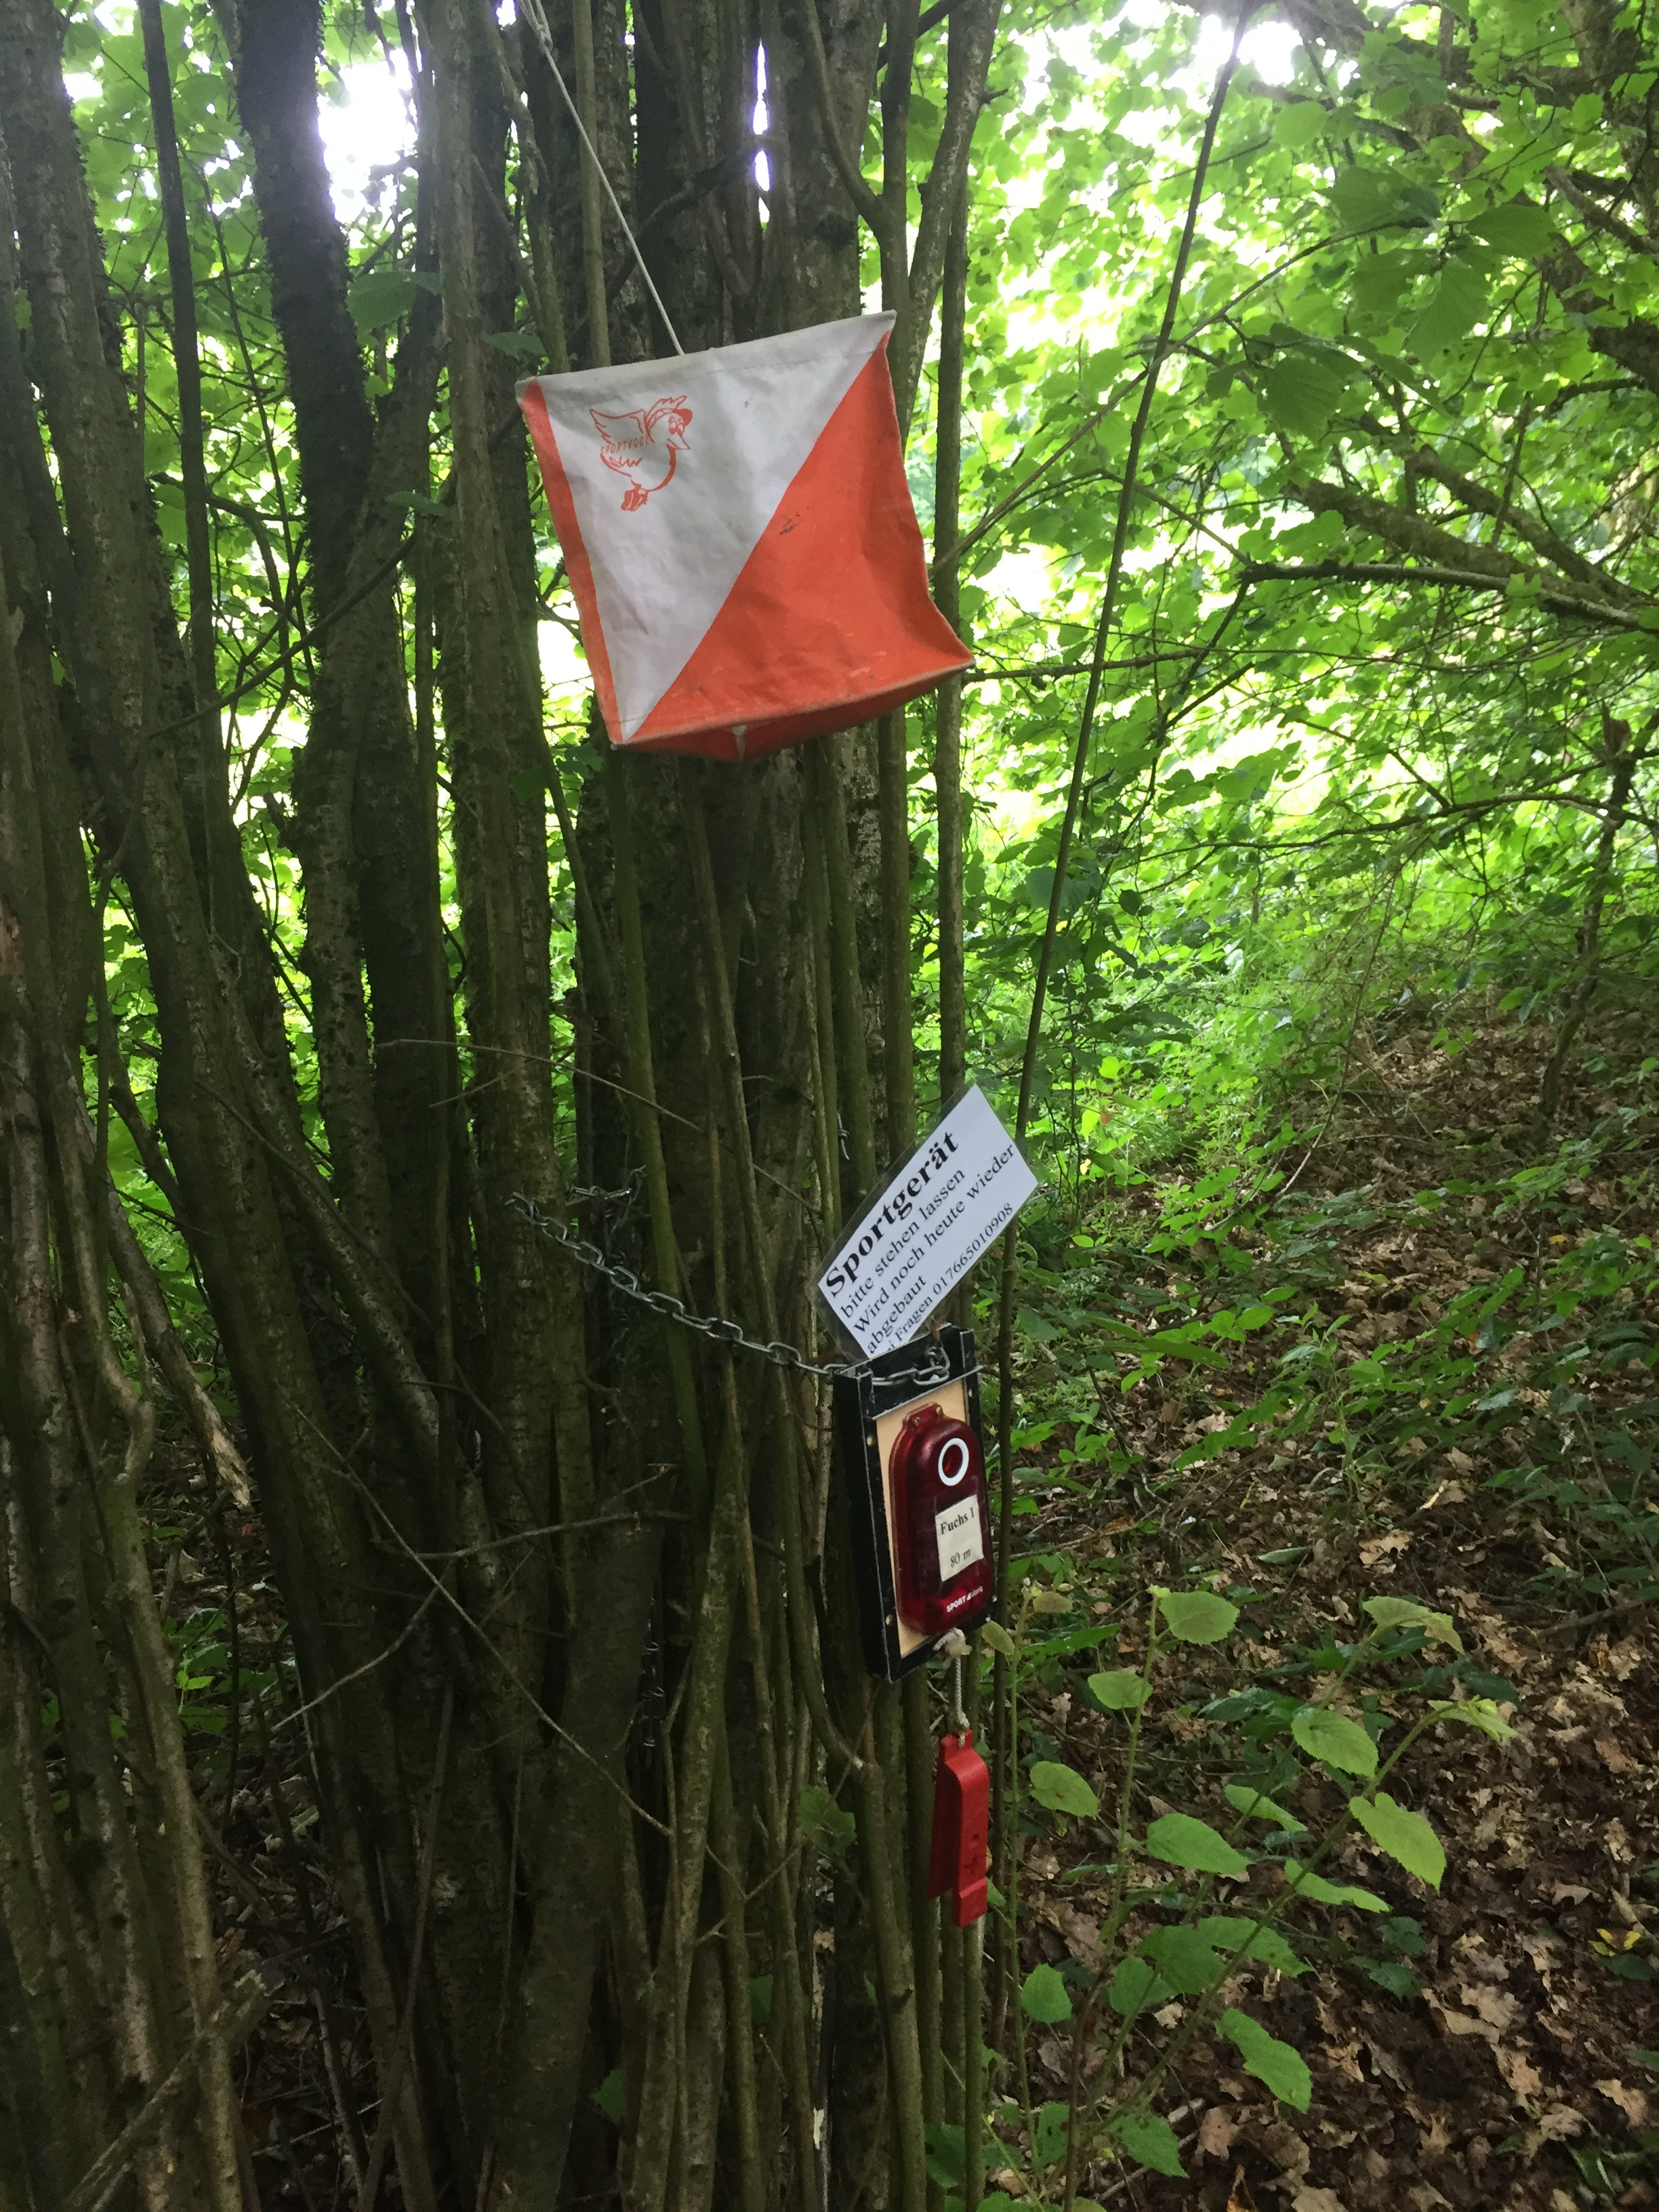
\includegraphics[width=0.85\textwidth]{foto/190}
    \caption{\scriptsize ARDF-Fuchs im Wald mit Wimpel und Zeitnehmer}
    \label{n_ardf_fuchs}
\end{figure}

   \end{column}
\end{columns}

\end{frame}

\begin{frame}
\only<1>{
\begin{QQuestion}{BE313}{Was verstehen Funkamateure unter einer \glqq Fuchsjagd\grqq{} (ARDF = Amateur Radio Direction Finding)?}{Es ist ein Funkwettbewerb, wobei versucht wird, in einer vorgegebenen Zeit auf einem Amateurfunkband mit möglichst vielen Ländern Funkverbindungen herzustellen.}
{Es ist ein Funkpeilwettbewerb, wobei mit Hilfe von tragbaren Peilempfängern versteckte Kleinsender im KW- oder UKW-Bereich, die nur kurzzeitig senden, aufzufinden sind.}
{Bei der Fuchsjagd wird versucht, den Weg von mobilen Kleinsendern zu verfolgen und dabei ein Muster zu erkennen.}
{Es ist ein Funkpeilwettbewerb, der von Funkamateuren ausschließlich für SWL's (short wave listeners) veranstaltet wird. }
\end{QQuestion}

}
\only<2>{
\begin{QQuestion}{BE313}{Was verstehen Funkamateure unter einer \glqq Fuchsjagd\grqq{} (ARDF = Amateur Radio Direction Finding)?}{Es ist ein Funkwettbewerb, wobei versucht wird, in einer vorgegebenen Zeit auf einem Amateurfunkband mit möglichst vielen Ländern Funkverbindungen herzustellen.}
{\textbf{\textcolor{DARCgreen}{Es ist ein Funkpeilwettbewerb, wobei mit Hilfe von tragbaren Peilempfängern versteckte Kleinsender im KW- oder UKW-Bereich, die nur kurzzeitig senden, aufzufinden sind.}}}
{Bei der Fuchsjagd wird versucht, den Weg von mobilen Kleinsendern zu verfolgen und dabei ein Muster zu erkennen.}
{Es ist ein Funkpeilwettbewerb, der von Funkamateuren ausschließlich für SWL's (short wave listeners) veranstaltet wird. }
\end{QQuestion}

}
\end{frame}

\begin{frame}
\only<1>{
\begin{QQuestion}{BD109}{Welche Kennungen werden von leistungsschwachen Amateurfunksendern zu Peilzwecken ausgesendet?}{MO, MOE, MOI, MOS, MOH oder MO5}
{DO, DOE, DOI, DOS, DOH oder DO5}
{DL, DL1, DL2, DL3, DL4 oder DL5}
{ARDF, ARDF1, ARDF2, ARDF3, ARDF4 oder ARDF5}
\end{QQuestion}

}
\only<2>{
\begin{QQuestion}{BD109}{Welche Kennungen werden von leistungsschwachen Amateurfunksendern zu Peilzwecken ausgesendet?}{\textbf{\textcolor{DARCgreen}{MO, MOE, MOI, MOS, MOH oder MO5}}}
{DO, DOE, DOI, DOS, DOH oder DO5}
{DL, DL1, DL2, DL3, DL4 oder DL5}
{ARDF, ARDF1, ARDF2, ARDF3, ARDF4 oder ARDF5}
\end{QQuestion}

}
\end{frame}%ENDCONTENT


\section{SSTV}
\label{section:sstv}
\begin{frame}%STARTCONTENT

\frametitle{Slow-Scan-Television (SSTV)}
\begin{itemize}
  \item Beim Slow-Scan-Television (SSTV) werden stehende Bilder mit geringer Auflösung übertragen.
  \item Rufzeichen und Rapporte werden bei SSTV einfach als Text in die Bilder reingeschrieben.
  \end{itemize}

\begin{figure}
    \includegraphics[width=0.85\textwidth]{foto/84}
    \caption{\scriptsize Ein per SSTV übertragenenes Bild}
    \label{n_sstv}
\end{figure}
\end{frame}

\begin{frame}
\only<1>{
\begin{QQuestion}{BE210}{Wie teilen Sie Ihrem Funkpartner in SSTV seinen \glqq Rapport\grqq{} mit?}{Ich teile ihm den Rapport später auf der QSL-Karte mit.}
{Ich schreibe den Rapport direkt in das zu übertragende Bild.}
{Ich sende den Rapport nach der Bildübertragung in CW.}
{Ich teile ihm den Rapport während der Bildübertragung in SSB mit.}
\end{QQuestion}

}
\only<2>{
\begin{QQuestion}{BE210}{Wie teilen Sie Ihrem Funkpartner in SSTV seinen \glqq Rapport\grqq{} mit?}{Ich teile ihm den Rapport später auf der QSL-Karte mit.}
{\textbf{\textcolor{DARCgreen}{Ich schreibe den Rapport direkt in das zu übertragende Bild.}}}
{Ich sende den Rapport nach der Bildübertragung in CW.}
{Ich teile ihm den Rapport während der Bildübertragung in SSB mit.}
\end{QQuestion}

}
\end{frame}%ENDCONTENT


\section{Notfunk}
\label{section:notfunk}
\begin{frame}%STARTCONTENT

\frametitle{Dürfen Funkamateure helfen?}
\begin{itemize}
  \item Ja! Funkamateure dürfen in Not- und Katastrophenfällen durch Übermittlung von Nachrichten für und an Dritte bei der Bewältigung einer Notlage unterstützen.
  \end{itemize}
\end{frame}

\begin{frame}
\only<1>{
\begin{QQuestion}{BF103}{Sie erreichen eine Unfallstelle. Der Ersthelfer bittet Sie, über Ihre mobile Amateurfunkstelle Hilfe zu holen, da das Mobiltelefonnetz nicht verfügbar ist. Wie verhalten Sie sich?}{Ich rufe per Funk einen Funkamateur und fordere diesen auf, die Polizei oder Rettungsleitstelle zu informieren.}
{Ich lehne es ab zu helfen, da im Amateurfunk keine Informationen für Dritte übermittelt werden dürfen.}
{Ich rufe per Funk mindestens dreimal MAYDAY gefolgt von meinem Rufzeichen, dem Standort und der Art der Notlage.}
{Ich lehne es ab zu helfen, da im Amateurfunk keine Notzeichen verwendet werden dürfen.}
\end{QQuestion}

}
\only<2>{
\begin{QQuestion}{BF103}{Sie erreichen eine Unfallstelle. Der Ersthelfer bittet Sie, über Ihre mobile Amateurfunkstelle Hilfe zu holen, da das Mobiltelefonnetz nicht verfügbar ist. Wie verhalten Sie sich?}{\textbf{\textcolor{DARCgreen}{Ich rufe per Funk einen Funkamateur und fordere diesen auf, die Polizei oder Rettungsleitstelle zu informieren.}}}
{Ich lehne es ab zu helfen, da im Amateurfunk keine Informationen für Dritte übermittelt werden dürfen.}
{Ich rufe per Funk mindestens dreimal MAYDAY gefolgt von meinem Rufzeichen, dem Standort und der Art der Notlage.}
{Ich lehne es ab zu helfen, da im Amateurfunk keine Notzeichen verwendet werden dürfen.}
\end{QQuestion}

}
\end{frame}

\begin{frame}
\frametitle{Was  tun, wenn man eine Notmeldung erhält?}
\begin{itemize}
  \item Bei einer Notmeldung sollte man zunächst aufmerksam zuhören und alle wichtigen Informationen notieren.
  \end{itemize}
\end{frame}

\begin{frame}
\only<1>{
\begin{QQuestion}{BF104}{Sie hören eine Notmeldung. Was tun Sie als Erstes?}{Ich wechsle die Frequenz oder schalte ab.}
{Ich sende dreimal MAYDAY, mein Rufzeichen und warte auf Antwort.}
{Ich stimme meinen Sender auf der Frequenz ab.}
{Ich höre aufmerksam zu und notiere alle wichtigen Informationen.}
\end{QQuestion}

}
\only<2>{
\begin{QQuestion}{BF104}{Sie hören eine Notmeldung. Was tun Sie als Erstes?}{Ich wechsle die Frequenz oder schalte ab.}
{Ich sende dreimal MAYDAY, mein Rufzeichen und warte auf Antwort.}
{Ich stimme meinen Sender auf der Frequenz ab.}
{\textbf{\textcolor{DARCgreen}{Ich höre aufmerksam zu und notiere alle wichtigen Informationen.}}}
\end{QQuestion}

}
\end{frame}

\begin{frame}
\frametitle{Was tun, wenn eine Rettungsorganisation sich der Sache annimmt?}
\begin{itemize}
  \item Wird die Notmeldung von einer Rettungsorganisation beantwortet, hält man sich zurück um den Funkbetrieb nicht zu stören.
  \end{itemize}
\end{frame}

\begin{frame}
\only<1>{
\begin{QQuestion}{BF105}{Sie haben eine Notmeldung aufgenommen, die nach kurzer Zeit von einer Rettungsorganisation beantwortet wird. Wie verhalten Sie sich?}{Ich bitte möglichst viele Funkamateure um Hilfe.}
{Ich biete zwischen zwei Durchgängen meine Hilfe an.}
{Ich stimme meinen Sender auf der Frequenz ab.}
{Ich störe auf keinen Fall den Funkbetrieb.}
\end{QQuestion}

}
\only<2>{
\begin{QQuestion}{BF105}{Sie haben eine Notmeldung aufgenommen, die nach kurzer Zeit von einer Rettungsorganisation beantwortet wird. Wie verhalten Sie sich?}{Ich bitte möglichst viele Funkamateure um Hilfe.}
{Ich biete zwischen zwei Durchgängen meine Hilfe an.}
{Ich stimme meinen Sender auf der Frequenz ab.}
{\textbf{\textcolor{DARCgreen}{Ich störe auf keinen Fall den Funkbetrieb.}}}
\end{QQuestion}

}
\end{frame}

\begin{frame}
\frametitle{Was tun, wenn zunächst niemand antwortet?}
\begin{itemize}
  \item Reagiert keine andere Funkstelle, beantwortet man den Ruf und informiert die Polizei oder Rettungsleitstelle.
  \end{itemize}
\end{frame}

\begin{frame}
\only<1>{
\begin{QQuestion}{BF106}{Sie haben eine Notmeldung aufgenommen. Keine andere Funkstelle reagiert und Sie könnten helfen. Wie verhalten Sie sich?}{Ich beantworte den Ruf und informiere die Polizei oder Rettungsleitstelle.}
{Ich schalte mein Funkgerät ab, um keine Probleme zu bekommen.}
{Ich wiederhole die Notmeldung umgehend auf derselben Frequenz.}
{Ich warte etwa eine Stunde, ob sich eine Rettungsorganisation meldet.}
\end{QQuestion}

}
\only<2>{
\begin{QQuestion}{BF106}{Sie haben eine Notmeldung aufgenommen. Keine andere Funkstelle reagiert und Sie könnten helfen. Wie verhalten Sie sich?}{\textbf{\textcolor{DARCgreen}{Ich beantworte den Ruf und informiere die Polizei oder Rettungsleitstelle.}}}
{Ich schalte mein Funkgerät ab, um keine Probleme zu bekommen.}
{Ich wiederhole die Notmeldung umgehend auf derselben Frequenz.}
{Ich warte etwa eine Stunde, ob sich eine Rettungsorganisation meldet.}
\end{QQuestion}

}
\end{frame}

\begin{frame}
\frametitle{Was tun, wenn man die zuständigen Stellen informiert hat?}
\begin{itemize}
  \item Idealerweise bleibt man erreichbar und gibt Informationen weiter, bis Hilfe eingetroffen ist.
  \end{itemize}
\end{frame}

\begin{frame}
\only<1>{
\begin{QQuestion}{BF107}{Sie haben eine Notmeldung beantwortet und die Polizei oder Rettungsleitstelle informiert. Welches Verhalten ist im Anschluss vorbildlich?}{Ich rufe regelmäßig die Polizei oder Rettungsleitstelle an und erkundige mich nach dem Stand.}
{Ich bleibe erreichbar und gebe Informationen weiter, bis Hilfe eingetroffen ist.}
{Ich schalte mein Funkgerät ab, da ich meiner Pflicht nachgekommen bin.}
{Ich informiere die Medien, damit über den Rettungseinsatz live berichtet werden kann.}
\end{QQuestion}

}
\only<2>{
\begin{QQuestion}{BF107}{Sie haben eine Notmeldung beantwortet und die Polizei oder Rettungsleitstelle informiert. Welches Verhalten ist im Anschluss vorbildlich?}{Ich rufe regelmäßig die Polizei oder Rettungsleitstelle an und erkundige mich nach dem Stand.}
{\textbf{\textcolor{DARCgreen}{Ich bleibe erreichbar und gebe Informationen weiter, bis Hilfe eingetroffen ist.}}}
{Ich schalte mein Funkgerät ab, da ich meiner Pflicht nachgekommen bin.}
{Ich informiere die Medien, damit über den Rettungseinsatz live berichtet werden kann.}
\end{QQuestion}

}
\end{frame}

\begin{frame}
\frametitle{Was ist bei internationaler Beteiligung zu beachten?}
\begin{itemize}
  \item Bei internationaler Beteiligung nutzt man UTC anstelle von lokaler Zeit.
  \end{itemize}
\end{frame}

\begin{frame}
\only<1>{
\begin{QQuestion}{BF108}{Sie haben am 16. August (Ortsdatum) um 20:00 Uhr mitteleuropäischer Sommerzeit (MESZ) von 9J2NG eine Notfunkmeldung aufgenommen und an eine Hilfeleistungsorganisation per Telefon weitergemeldet. Die Amateurfunkstelle 9J2NG hat Sie gebeten, um 23:00 Uhr UTC erneut mit ihr in Verbindung zu treten. Welcher Zeitpunkt ist dies in Deutschland?}{22:00 MESZ am 16. August (Ortsdatum)}
{21:00 MESZ am 16. August (Ortsdatum)}
{01:00 MESZ am 17. August (Ortsdatum)}
{00:00 MESZ am 18. August (Ortsdatum)}
\end{QQuestion}

}
\only<2>{
\begin{QQuestion}{BF108}{Sie haben am 16. August (Ortsdatum) um 20:00 Uhr mitteleuropäischer Sommerzeit (MESZ) von 9J2NG eine Notfunkmeldung aufgenommen und an eine Hilfeleistungsorganisation per Telefon weitergemeldet. Die Amateurfunkstelle 9J2NG hat Sie gebeten, um 23:00 Uhr UTC erneut mit ihr in Verbindung zu treten. Welcher Zeitpunkt ist dies in Deutschland?}{22:00 MESZ am 16. August (Ortsdatum)}
{21:00 MESZ am 16. August (Ortsdatum)}
{\textbf{\textcolor{DARCgreen}{01:00 MESZ am 17. August (Ortsdatum)}}}
{00:00 MESZ am 18. August (Ortsdatum)}
\end{QQuestion}

}
\end{frame}

\begin{frame}
\frametitle{Notzeichen}
\begin{itemize}
  \item Die Notzeichen außerhalb des Amateurfunks sind SOS und Mayday, diese dürfen im Amateurfunk nicht verwendet werden.
  \end{itemize}

\end{frame}

\begin{frame}
\only<1>{
\begin{QQuestion}{VD105}{Dürfen im Amateurfunkverkehr internationale Not-, Dringlichkeits- und Sicherheitszeichen (z. B. MAYDAY, PAN PAN, SÉCURITÉ) ausgesendet werden?}{Der Gebrauch dieser Zeichen ist auf den Kurzwellenbändern erlaubt.}
{Amateurfunkstellen in Küstennähe ist es erlaubt, diese Zeichen auszusenden.}
{Bei einem Notfall dürfen die Zeichen ausgesendet werden.}
{Der Gebrauch dieser Zeichen ist ausdrücklich untersagt.}
\end{QQuestion}

}
\only<2>{
\begin{QQuestion}{VD105}{Dürfen im Amateurfunkverkehr internationale Not-, Dringlichkeits- und Sicherheitszeichen (z. B. MAYDAY, PAN PAN, SÉCURITÉ) ausgesendet werden?}{Der Gebrauch dieser Zeichen ist auf den Kurzwellenbändern erlaubt.}
{Amateurfunkstellen in Küstennähe ist es erlaubt, diese Zeichen auszusenden.}
{Bei einem Notfall dürfen die Zeichen ausgesendet werden.}
{\textbf{\textcolor{DARCgreen}{Der Gebrauch dieser Zeichen ist ausdrücklich untersagt.}}}
\end{QQuestion}

}
\end{frame}

\begin{frame}
\only<1>{
\begin{QQuestion}{BF101}{Wie heißen die internationalen Notzeichen außerhalb des Amateurfunks?}{Prudence und TTT}
{Securité und Distresse}
{Distresse und DDD}
{Mayday und SOS}
\end{QQuestion}

}
\only<2>{
\begin{QQuestion}{BF101}{Wie heißen die internationalen Notzeichen außerhalb des Amateurfunks?}{Prudence und TTT}
{Securité und Distresse}
{Distresse und DDD}
{\textbf{\textcolor{DARCgreen}{Mayday und SOS}}}
\end{QQuestion}

}
\end{frame}

\begin{frame}
\only<1>{
\begin{QQuestion}{BF102}{Dürfen Sie im Notfall SOS oder Mayday innerhalb des Amateurfunks gebrauchen?}{SOS nicht, aber Mayday im Notfall.}
{Mayday nicht, aber SOS im Notfall.}
{Ja}
{Nein}
\end{QQuestion}

}
\only<2>{
\begin{QQuestion}{BF102}{Dürfen Sie im Notfall SOS oder Mayday innerhalb des Amateurfunks gebrauchen?}{SOS nicht, aber Mayday im Notfall.}
{Mayday nicht, aber SOS im Notfall.}
{Ja}
{\textbf{\textcolor{DARCgreen}{Nein}}}
\end{QQuestion}

}
\end{frame}

\begin{frame}
\frametitle{ Notfunkfrequenzen}
Die IARU hat für die ITU-Region 1 die folgenden Notfunkfrequenzen in den Bandplänen festgelegt, die für den Notfunkbetrieb frei zu halten sind:

\begin{itemize}
  \item 3.\qty{760}{\kilo\hertz}
  \item 7.\qty{110}{\kilo\hertz}
  \item 14.\qty{300}{\kilo\hertz}
  \item 18.\qty{160}{\kilo\hertz}
  \item 21.\qty{360}{\kilo\hertz}
  \end{itemize}
\end{frame}%ENDCONTENT


\title{DARC Amateurfunklehrgang Klasse NEA}
\author{Antennen und Übertragungsleitungen}
\institute{Deutscher Amateur Radio Club e.\,V.}
\begin{frame}
\maketitle
\end{frame}

\section{Antennen}
\label{section:antennen}
\begin{frame}%STARTCONTENT

\begin{figure}
    \DARCimage{0.85\linewidth}{657include}
    \caption{\scriptsize Schematische Darstellung einer Amateurfunkstation mit Funkgerät, Speiseleitung und Antenne}
    \label{n_trx_kabel_und_antenne}
\end{figure}
\begin{columns}
    \begin{column}{0.48\textwidth}
    \begin{itemize}
  \item Gibt elektrische Schwingungen als Funkwellen ab
  \item Funkwellen breiten sich in der Ferne aus
  \end{itemize}

    \end{column}
   \begin{column}{0.48\textwidth}
       \begin{itemize}
  \item Nimmt beim Empfang Funkwellen auf
  \item Leitet sie als elektrische Schwingungen über das Antennenkabel zum Funkgerät
  \end{itemize}

   \end{column}
\end{columns}

\end{frame}

\begin{frame}
\only<1>{
\begin{PQuestion}{NG101}{Welches Bauteil wird durch das Schaltzeichen symbolisiert?}{Diode}
{Erde}
{Antenne}
{Transistor}
{\DARCimage{0.1\linewidth}{543include}}\end{PQuestion}

}
\only<2>{
\begin{PQuestion}{NG101}{Welches Bauteil wird durch das Schaltzeichen symbolisiert?}{Diode}
{Erde}
{\textbf{\textcolor{DARCgreen}{Antenne}}}
{Transistor}
{\DARCimage{0.1\linewidth}{543include}}\end{PQuestion}

}
\end{frame}%ENDCONTENT


\section{Dipol-Antenne}
\label{section:dipol}
\begin{frame}%STARTCONTENT

\begin{figure}
    \DARCimage{0.85\linewidth}{589include}
    \caption{\scriptsize Darstellung einer Dipol-Antenne}
    \label{n_dipol}
\end{figure}
\begin{columns}
    \begin{column}{0.48\textwidth}
    \begin{itemize}
  \item In der Praxis wird häufig der Halbwellendipol verwendet
  \item Ist eine halbe Wellenlänge lang
  \end{itemize}

    \end{column}
   \begin{column}{0.48\textwidth}
       
    \pause
    Beispiel:

\begin{itemize}
  \item Wellenlänge von \qty{10}{\metre}
  \item halbe Wellenlänge \qty{5}{\metre}
  \item Jedes Teilstück des Dipols \qty{2,5}{\metre}
  \end{itemize}



   \end{column}
\end{columns}

\end{frame}

\begin{frame}
\only<1>{
\begin{PQuestion}{NG103}{Wie wird die dargestellte Antenne bezeichnet?}{Endgespeiste Antenne}
{Groundplane-Antenne}
{Dipol-Antenne}
{Yagi-Uda-Antenne}
{\DARCimage{1.0\linewidth}{589include}}\end{PQuestion}

}
\only<2>{
\begin{PQuestion}{NG103}{Wie wird die dargestellte Antenne bezeichnet?}{Endgespeiste Antenne}
{Groundplane-Antenne}
{\textbf{\textcolor{DARCgreen}{Dipol-Antenne}}}
{Yagi-Uda-Antenne}
{\DARCimage{1.0\linewidth}{589include}}\end{PQuestion}

}
\end{frame}

\begin{frame}
\frametitle{Anpassung}
Dipol-Antenne auf die gewünschte Frequenz bringen durch gleichmäßiges Kürzen oder Verlängern

\begin{itemize}
  \item Zu hohe Resonanzfrequenz: Beide Seiten gleichmäßig verlängern
  \item Zu niedrige Resonanzfrequenz: Beide Seiten gleichmäßig verkürzen
  \end{itemize}
\end{frame}

\begin{frame}
\only<1>{
\begin{QQuestion}{NG304}{Ihre selbstgebaute Dipol-Antenne ist unterhalb der gewünschten Frequenz resonant. Welche Änderung können Sie vornehmen, um die Resonanz in den gewünschten Bereich zu bringen?}{Sendeleistung verringern}
{Beide Enden gleichmäßig verlängern}
{Sendeleistung erhöhen}
{Beide Enden gleichmäßig kürzen}
\end{QQuestion}

}
\only<2>{
\begin{QQuestion}{NG304}{Ihre selbstgebaute Dipol-Antenne ist unterhalb der gewünschten Frequenz resonant. Welche Änderung können Sie vornehmen, um die Resonanz in den gewünschten Bereich zu bringen?}{Sendeleistung verringern}
{Beide Enden gleichmäßig verlängern}
{Sendeleistung erhöhen}
{\textbf{\textcolor{DARCgreen}{Beide Enden gleichmäßig kürzen}}}
\end{QQuestion}

}
\end{frame}

\begin{frame}
\only<1>{
\begin{QQuestion}{NG305}{Ihre selbstgebaute Dipol-Antenne ist oberhalb der gewünschten Frequenz resonant. Welche Änderung können Sie vornehmen, um die Resonanz in den gewünschten Bereich zu bringen?}{Sendeleistung erhöhen}
{Beide Enden gleichmäßig kürzen}
{Beide Enden gleichmäßig verlängern}
{Sendeleistung verringern}
\end{QQuestion}

}
\only<2>{
\begin{QQuestion}{NG305}{Ihre selbstgebaute Dipol-Antenne ist oberhalb der gewünschten Frequenz resonant. Welche Änderung können Sie vornehmen, um die Resonanz in den gewünschten Bereich zu bringen?}{Sendeleistung erhöhen}
{Beide Enden gleichmäßig kürzen}
{\textbf{\textcolor{DARCgreen}{Beide Enden gleichmäßig verlängern}}}
{Sendeleistung verringern}
\end{QQuestion}

}
\end{frame}%ENDCONTENT


\section{Yagi-Uda-Antenne}
\label{section:yagi_uda_1}
\begin{frame}%STARTCONTENT

\begin{columns}
    \begin{column}{0.48\textwidth}
    
\begin{figure}
    \DARCimage{0.85\linewidth}{613include}
    \caption{\scriptsize Yagi-Uda-Antenne mit Einspeisung am Dipol am vorletzten Element}
    \label{n_yagi_uda}
\end{figure}


    \end{column}
   \begin{column}{0.48\textwidth}
       \begin{itemize}
  \item Vor und hinter dem Dipol werden leitende Stäbe geschickt angeordnet
  \item Bündelt Funkwellen in eine bestimmte Richtung
  \end{itemize}

   \end{column}
\end{columns}

\end{frame}

\begin{frame}
\only<1>{
\begin{PQuestion}{NG108}{Wie wird die dargestellte Antenne bezeichnet?}{Dipol-Antenne}
{Yagi-Uda-Antenne}
{Groundplane-Antenne}
{Endgespeiste Antenne}
{\DARCimage{0.5\linewidth}{613include}}\end{PQuestion}

}
\only<2>{
\begin{PQuestion}{NG108}{Wie wird die dargestellte Antenne bezeichnet?}{Dipol-Antenne}
{\textbf{\textcolor{DARCgreen}{Yagi-Uda-Antenne}}}
{Groundplane-Antenne}
{Endgespeiste Antenne}
{\DARCimage{0.5\linewidth}{613include}}\end{PQuestion}

}
\end{frame}%ENDCONTENT


\section{Rundstrahlantennen}
\label{section:rundstrahler}
\begin{frame}%STARTCONTENT
Ein Dipolschenkel wird durch eine Erdung (Ground) oder große Metallfläche (Fahrzeug) ersetzt
\begin{columns}
    \begin{column}{0.48\textwidth}
    
\begin{figure}
    \DARCimage{0.85\linewidth}{669include}
    \caption{\scriptsize Marconi-Antenne}
    \label{n_marconi_antenne}
\end{figure}


    \end{column}
   \begin{column}{0.48\textwidth}
       Erdung kann durch \emph{Radials} ersetzt werden, die eine \emph{Groundplane} bilden


   \end{column}
\end{columns}

\end{frame}

\begin{frame}
\only<1>{
\begin{PQuestion}{NG105}{Wie wird die dargestellte Antenne bezeichnet?}{Groundplane-Antenne}
{Yagi-Uda-Antenne}
{Dipol-Antenne}
{Endgespeiste Antenne}
{\DARCimage{0.5\linewidth}{614include}}\end{PQuestion}

}
\only<2>{
\begin{PQuestion}{NG105}{Wie wird die dargestellte Antenne bezeichnet?}{\textbf{\textcolor{DARCgreen}{Groundplane-Antenne}}}
{Yagi-Uda-Antenne}
{Dipol-Antenne}
{Endgespeiste Antenne}
{\DARCimage{0.5\linewidth}{614include}}\end{PQuestion}

}
\end{frame}

\begin{frame}
\only<1>{
\begin{QQuestion}{NG106}{Die elektrischen Gegengewichte einer Groundplane-Antenne bezeichnet man auch als~...}{Erdelemente.}
{Reflektoren.}
{Direktoren.}
{Radials.}
\end{QQuestion}

}
\only<2>{
\begin{QQuestion}{NG106}{Die elektrischen Gegengewichte einer Groundplane-Antenne bezeichnet man auch als~...}{Erdelemente.}
{Reflektoren.}
{Direktoren.}
{\textbf{\textcolor{DARCgreen}{Radials.}}}
\end{QQuestion}

}
\end{frame}

\begin{frame}
\only<1>{
\begin{QQuestion}{NG104}{Eine Marconi-Antenne ist~...}{eine vertikale Halbwellenantenne.}
{eine 5/8-$\lambda$-Antenne mit abgestimmten Radials.}
{eine horizontale $\lambda$/2-Langdrahtantenne.}
{eine gegen Erde erregte $\lambda$/4-Vertikalantenne.}
\end{QQuestion}

}
\only<2>{
\begin{QQuestion}{NG104}{Eine Marconi-Antenne ist~...}{eine vertikale Halbwellenantenne.}
{eine 5/8-$\lambda$-Antenne mit abgestimmten Radials.}
{eine horizontale $\lambda$/2-Langdrahtantenne.}
{\textbf{\textcolor{DARCgreen}{eine gegen Erde erregte $\lambda$/4-Vertikalantenne.}}}
\end{QQuestion}

}
\end{frame}

\begin{frame}
\only<1>{
\begin{PQuestion}{NG102}{Was wird durch dieses Schaltzeichen symbolisiert?}{Erde}
{Antenne}
{Diode}
{Batterie}
{\DARCimage{0.1\linewidth}{544include}}\end{PQuestion}

}
\only<2>{
\begin{PQuestion}{NG102}{Was wird durch dieses Schaltzeichen symbolisiert?}{\textbf{\textcolor{DARCgreen}{Erde}}}
{Antenne}
{Diode}
{Batterie}
{\DARCimage{0.1\linewidth}{544include}}\end{PQuestion}

}
\end{frame}

\begin{frame}
\only<1>{
\begin{QQuestion}{NG110}{Welche Antenne ist für eine \qty{2}{\m}-QSO-Runde mit im Umkreis verteilten Funkamateuren am besten geeignet?}{Ferritantenne}
{Yagi-Uda-Antenne}
{Rundstrahlantenne}
{Langdrahtantenne}
\end{QQuestion}

}
\only<2>{
\begin{QQuestion}{NG110}{Welche Antenne ist für eine \qty{2}{\m}-QSO-Runde mit im Umkreis verteilten Funkamateuren am besten geeignet?}{Ferritantenne}
{Yagi-Uda-Antenne}
{\textbf{\textcolor{DARCgreen}{Rundstrahlantenne}}}
{Langdrahtantenne}
\end{QQuestion}

}
\end{frame}

\begin{frame}
\only<1>{
\begin{QQuestion}{NG111}{Welche Antennenkonfiguration ist zu wählen, wenn möglichst viele umliegende Relaisstationen im \qty{2}{\m}- oder im \qty{70}{\cm}-Band erreicht werden sollen?}{Eine Ferritantenne auf der Fensterbank.}
{Ein Rundstrahler auf dem Hausdach.}
{Eine in einer Richtung fest montierte horizontale Richtantenne.}
{Eine Magnetfußantenne auf dem Dachboden.}
\end{QQuestion}

}
\only<2>{
\begin{QQuestion}{NG111}{Welche Antennenkonfiguration ist zu wählen, wenn möglichst viele umliegende Relaisstationen im \qty{2}{\m}- oder im \qty{70}{\cm}-Band erreicht werden sollen?}{Eine Ferritantenne auf der Fensterbank.}
{\textbf{\textcolor{DARCgreen}{Ein Rundstrahler auf dem Hausdach.}}}
{Eine in einer Richtung fest montierte horizontale Richtantenne.}
{Eine Magnetfußantenne auf dem Dachboden.}
\end{QQuestion}

}
\end{frame}%ENDCONTENT


\section{Endgespeiste Antennen (End-Fed)}
\label{section:endgespeiste_antennen}
\begin{frame}%STARTCONTENT

\begin{figure}
    \DARCimage{0.85\linewidth}{615include}
    \caption{\scriptsize Schaltbild einer endgespeisten Antenne}
    \label{n_antennenformen_schaltbild_endfed}
\end{figure}

\begin{itemize}
  \item Statt in der Mitte das Antennenkabel an einem Ende des Dipols anschließen
  \item Häufige Bauform: Endgespeister Halbwellendipol
  \item Ist der Draht einer endgespeisten Antenne länger als die Wellenlänge: Langdraht-Antenne
  \end{itemize}
\end{frame}

\begin{frame}
\only<1>{
\begin{PQuestion}{NG107}{Wie wird die dargestellte Antenne bezeichnet?}{Endgespeiste Antenne}
{Groundplane-Antenne}
{Dipol-Antenne}
{Yagi-Uda-Antenne}
{\DARCimage{1.0\linewidth}{615include}}\end{PQuestion}

}
\only<2>{
\begin{PQuestion}{NG107}{Wie wird die dargestellte Antenne bezeichnet?}{\textbf{\textcolor{DARCgreen}{Endgespeiste Antenne}}}
{Groundplane-Antenne}
{Dipol-Antenne}
{Yagi-Uda-Antenne}
{\DARCimage{1.0\linewidth}{615include}}\end{PQuestion}

}
\end{frame}

\begin{frame}
\only<1>{
\begin{QQuestion}{NG109}{Welche Antennenform wird von Funkamateuren in der Regel nur im Kurzwellenbereich und \underline{nicht} im VHF/UHF-Bereich verwendet?}{Langdraht-Antenne}
{Yagi-Uda-Antenne}
{Quad-Antenne}
{Groundplane-Antenne}
\end{QQuestion}

}
\only<2>{
\begin{QQuestion}{NG109}{Welche Antennenform wird von Funkamateuren in der Regel nur im Kurzwellenbereich und \underline{nicht} im VHF/UHF-Bereich verwendet?}{\textbf{\textcolor{DARCgreen}{Langdraht-Antenne}}}
{Yagi-Uda-Antenne}
{Quad-Antenne}
{Groundplane-Antenne}
\end{QQuestion}

}
\end{frame}%ENDCONTENT


\section{Polarisation}
\label{section:polarisation}
\begin{frame}%STARTCONTENT

\begin{columns}
    \begin{column}{0.48\textwidth}
    \begin{itemize}
  \item Polarisation kann \emph{vertikal} oder \emph{horizontal} sein
  \item Lässt sich bei den meisten Antennen leicht erkennen
  \item Auf VHF und höher sollten alle die gleiche Polarisation verwenden
  \end{itemize}

    \end{column}
   \begin{column}{0.48\textwidth}
       \begin{itemize}
  \item \emph{Zirkular} polarisiert
  \item Drehende Funkwellen mit besonderer Antennenbauform
  \item Unterscheidung in \enquote{linkszirkular} und \enquote{rechtszirkular} polarisiert
  \end{itemize}

   \end{column}
\end{columns}

\end{frame}

\begin{frame}
\only<1>{
\begin{QQuestion}{NB304}{Welche Polarisationen unterscheidet man üblicherweise bei der Funkwellenausbreitung im Amateurfunk und wieso sollte man diese beachten?}{Man unterscheidet parallele, koaxiale und drahtlose Polarisation. Die Polarisation der Antennenkabel muss auf die Antennen abgestimmt sein, um Verluste zu minimieren.}
{Man unterscheidet transversale, longitudinale und orthogonale Polarisation. Die Polarisation des Funkgeräts muss an das Stromnetz angepasst sein, um Kurzschlüsse zu vermeiden.}
{Man unterscheidet kohärente, inkohärente und korrelierte Polarisation. Die Polarisation der Funkwellen sollte regelmäßig geändert werden, um die Störfestigkeit zu erhöhen.}
{Man unterscheidet horizontale, vertikale sowie links- und rechtszirkulare Polarisation. Die Polarisation von Sende- und Empfangsantenne sollten angeglichen sein, um eine verlustarme Übertragung zu gewährleisten.}
\end{QQuestion}

}
\only<2>{
\begin{QQuestion}{NB304}{Welche Polarisationen unterscheidet man üblicherweise bei der Funkwellenausbreitung im Amateurfunk und wieso sollte man diese beachten?}{Man unterscheidet parallele, koaxiale und drahtlose Polarisation. Die Polarisation der Antennenkabel muss auf die Antennen abgestimmt sein, um Verluste zu minimieren.}
{Man unterscheidet transversale, longitudinale und orthogonale Polarisation. Die Polarisation des Funkgeräts muss an das Stromnetz angepasst sein, um Kurzschlüsse zu vermeiden.}
{Man unterscheidet kohärente, inkohärente und korrelierte Polarisation. Die Polarisation der Funkwellen sollte regelmäßig geändert werden, um die Störfestigkeit zu erhöhen.}
{\textbf{\textcolor{DARCgreen}{Man unterscheidet horizontale, vertikale sowie links- und rechtszirkulare Polarisation. Die Polarisation von Sende- und Empfangsantenne sollten angeglichen sein, um eine verlustarme Übertragung zu gewährleisten.}}}
\end{QQuestion}

}
\end{frame}%ENDCONTENT


\section{Polarisation II}
\label{section:polarisation_2}
\begin{frame}%STARTCONTENT
\begin{itemize}
  \item Polarisation einer Antenne bezieht sich auf die Ausrichtung des elektrischen Feldes
  \item In Hauptstrahlrichtung
  \item In Bezug zur Erdoberfläche
  \item Die Polarisationsrichtung kann nicht immer an der Bauform der Antenne erkannt werden
  \end{itemize}

\end{frame}

\begin{frame}
\only<1>{
\begin{QQuestion}{EG222}{Die Polarisation einer Antenne~...}{wird nach der Ausrichtung der magnetischen Feldkomponente in der Hauptstrahlrichtung in Bezug zur Erdoberfläche angegeben.}
{wird nach der Ausrichtung der elektrischen Feldkomponente in der Hauptstrahlrichtung in Bezug zur Erdoberfläche angegeben.}
{entspricht der Richtung der magnetischen Feldkomponente des empfangenen oder ausgesendeten Feldes in Bezug auf die Nordrichtung (Azimut).}
{entspricht der Richtung der elektrischen Feldkomponente des empfangenen oder ausgesendeten Feldes in Bezug auf die Nordrichtung (Azimut).}
\end{QQuestion}

}
\only<2>{
\begin{QQuestion}{EG222}{Die Polarisation einer Antenne~...}{wird nach der Ausrichtung der magnetischen Feldkomponente in der Hauptstrahlrichtung in Bezug zur Erdoberfläche angegeben.}
{\textbf{\textcolor{DARCgreen}{wird nach der Ausrichtung der elektrischen Feldkomponente in der Hauptstrahlrichtung in Bezug zur Erdoberfläche angegeben.}}}
{entspricht der Richtung der magnetischen Feldkomponente des empfangenen oder ausgesendeten Feldes in Bezug auf die Nordrichtung (Azimut).}
{entspricht der Richtung der elektrischen Feldkomponente des empfangenen oder ausgesendeten Feldes in Bezug auf die Nordrichtung (Azimut).}
\end{QQuestion}

}
\end{frame}%ENDCONTENT


\section{Polarisation III}
\label{section:polarisation_3}
\begin{frame}%STARTCONTENT

\only<1>{
\begin{QQuestion}{AG201}{Mit welcher Polarisation wird auf den Kurzwellenbändern meistens gesendet?}{Es wird nur mit horizontaler Polarisation gesendet.}
{Es wird meistens mit horizontaler oder zirkularer Polarisation gesendet.}
{Es wird meistens mit vertikaler oder zirkularer Polarisation gesendet.}
{Es wird meistens mit horizontaler oder vertikaler Polarisation gesendet.}
\end{QQuestion}

}
\only<2>{
\begin{QQuestion}{AG201}{Mit welcher Polarisation wird auf den Kurzwellenbändern meistens gesendet?}{Es wird nur mit horizontaler Polarisation gesendet.}
{Es wird meistens mit horizontaler oder zirkularer Polarisation gesendet.}
{Es wird meistens mit vertikaler oder zirkularer Polarisation gesendet.}
{\textbf{\textcolor{DARCgreen}{Es wird meistens mit horizontaler oder vertikaler Polarisation gesendet.}}}
\end{QQuestion}

}
\end{frame}%ENDCONTENT


\section{Antennenformen II}
\label{section:antennenformen_2}
\begin{frame}%STARTCONTENT

\frametitle{Symmetrie}
\begin{itemize}
  \item Mittengespeiste Dipole sind \emph{symmetrische Antennen}
  \item Weist an beiden Polen (z.B. den Einspeisepunkten) bis auf das Vorzeichen die gleiche Spannung gegenüber Erde auf
  \item Bei Dipolen und darauf basierenden Yagi-Uda-Antennen der Fall
  \item Die Groundplane-Antenne ist \emph{unsymmetrisch}, da sie am Anschlusspunkt der Radiale Erdpotential hat
  \end{itemize}

\end{frame}

\begin{frame}
\only<1>{
\begin{QQuestion}{EG213}{Welche Antenne gehört \underline{nicht} zu den symmetrischen Antennen?}{mittengespeister $\lambda$/2-Dipol}
{Faltdipol}
{Lang-Yagi-Uda}
{Groundplane}
\end{QQuestion}

}
\only<2>{
\begin{QQuestion}{EG213}{Welche Antenne gehört \underline{nicht} zu den symmetrischen Antennen?}{mittengespeister $\lambda$/2-Dipol}
{Faltdipol}
{Lang-Yagi-Uda}
{\textbf{\textcolor{DARCgreen}{Groundplane}}}
\end{QQuestion}

}
\end{frame}

\begin{frame}
\frametitle{Schleifenantennen}
\begin{itemize}
  \item Draht von insgesamt etwa einer Wellenlänge
  \item In Form eines Kreises, Quadrats, Dreiecks, …
  \item Beliebt: Delta-Loop-Antenne in Form eines Delta (Δ), da nur ein Mast benötigt wird
  \end{itemize}
\end{frame}

\begin{frame}
\only<1>{
\begin{QQuestion}{EG101}{Wie nennt man eine Schleifenantenne, die aus drei gleich langen Drahtstücken besteht?}{3-Element-Beam}
{3-Element-Quad-Loop-Antenne}
{W3DZZ-Antenne}
{Delta-Loop-Antenne}
\end{QQuestion}

}
\only<2>{
\begin{QQuestion}{EG101}{Wie nennt man eine Schleifenantenne, die aus drei gleich langen Drahtstücken besteht?}{3-Element-Beam}
{3-Element-Quad-Loop-Antenne}
{W3DZZ-Antenne}
{\textbf{\textcolor{DARCgreen}{Delta-Loop-Antenne}}}
\end{QQuestion}

}
\end{frame}

\begin{frame}
\frametitle{Magnetic-Loop}
\begin{itemize}
  \item Magnetische Ringantenne, da Abstrahlung im Nahfeld über das Magnetfeld erfolgt
  \item Ca. $\frac{\lambda}{10}$ Umfang
  \item Wirkungsgrad bei \qty{1}{\percent}-\qty{10}{\percent} im Sendebetrieb
  \item Weniger Störungen bei elektrisch leitfähigen oder dämpfenden Gegenständen im Nahfeld
  \end{itemize}

\end{frame}

\begin{frame}
\only<1>{
\begin{QQuestion}{EG105}{Welche Antennenform eignet sich für Sendebetrieb und weist dabei im Nahfeld ein starkes magnetisches Feld auf?}{Eine Cubical-Quad-Antenne}
{Eine Ferritstabantenne}
{Ein Faltdipol}
{Eine magnetische Ringantenne mit einem Umfang von etwa $\lambda$/10}
\end{QQuestion}

}
\only<2>{
\begin{QQuestion}{EG105}{Welche Antennenform eignet sich für Sendebetrieb und weist dabei im Nahfeld ein starkes magnetisches Feld auf?}{Eine Cubical-Quad-Antenne}
{Eine Ferritstabantenne}
{Ein Faltdipol}
{\textbf{\textcolor{DARCgreen}{Eine magnetische Ringantenne mit einem Umfang von etwa $\lambda$/10}}}
\end{QQuestion}

}
\end{frame}

\begin{frame}
\frametitle{Endgespeiste Antennen}
\begin{itemize}
  \item Speisung vom Ende her
  \item Länge häufig $\frac{\lambda}{2}$
  \item Benötigt eine höhere Spannung
  \end{itemize}
\end{frame}

\begin{frame}
\frametitle{Fuchs-Antenne}
\begin{columns}
    \begin{column}{0.48\textwidth}
    \begin{itemize}
  \item Verwendung eines Anpassglieds (Transformator)
  \item Oft verwendet: Fuchskreis
  \end{itemize}

    \end{column}
   \begin{column}{0.48\textwidth}
       
\begin{figure}
    \DARCimage{0.85\linewidth}{310include}
    \caption{\scriptsize Schematische Darstellung einer Fuchs-Antenne mit Fuchskreis}
    \label{e_antennenformen_fuchskreis}
\end{figure}


   \end{column}
\end{columns}

\end{frame}

\begin{frame}
\only<1>{
\begin{PQuestion}{EG104}{Welche Antennenart ist hier dargestellt?  }{Dipol-Antenne}
{Windom-Antenne}
{Fuchs-Antenne}
{Groundplane-Antenne}
{\DARCimage{1.0\linewidth}{310include}}\end{PQuestion}

}
\only<2>{
\begin{PQuestion}{EG104}{Welche Antennenart ist hier dargestellt?  }{Dipol-Antenne}
{Windom-Antenne}
{\textbf{\textcolor{DARCgreen}{Fuchs-Antenne}}}
{Groundplane-Antenne}
{\DARCimage{1.0\linewidth}{310include}}\end{PQuestion}

}
\end{frame}

\begin{frame}
\only<1>{
\begin{PQuestion}{EG103}{Welche Antenne ist hier dargestellt?}{Einband-Drahtantenne mit Preselektor}
{Einseitig geerdeter Winkeldipol mit Oberwellenfilter}
{Endgespeiste Antenne mit Collins-Filter zur Anpassung}
{Endgespeiste Antenne mit einfachem Anpassglied}
{\DARCimage{1.0\linewidth}{310include}}\end{PQuestion}

}
\only<2>{
\begin{PQuestion}{EG103}{Welche Antenne ist hier dargestellt?}{Einband-Drahtantenne mit Preselektor}
{Einseitig geerdeter Winkeldipol mit Oberwellenfilter}
{Endgespeiste Antenne mit Collins-Filter zur Anpassung}
{\textbf{\textcolor{DARCgreen}{Endgespeiste Antenne mit einfachem Anpassglied}}}
{\DARCimage{1.0\linewidth}{310include}}\end{PQuestion}

}
\end{frame}

\begin{frame}
\frametitle{Richtwirkung}
\begin{itemize}
  \item Darstellung als \emph{Strahlungsdiagramm}
  \item Für eine Ebene wird in jede Richtung der Gewinn bzw. Feldstärke oder Strahlungsleistung aufgetragen
  \item Je weiter der Graphenverlauf vom Mittelpunkt entfernt ist, umso größer der Gewinn bzw. umso höher die Feldstärke und Strahlungsleistung im Fernfeld
  \item Oft wird Antenne mit darin dargestellt
  \end{itemize}
\end{frame}

\begin{frame}
\frametitle{Richtwirkung eines Dipols}
\begin{columns}
    \begin{column}{0.48\textwidth}
    \begin{itemize}
  \item Strahlt rechtwinklig vom Draht ab
  \item In einer Ebene betrachtet ergeben sich Keulen neben dem Dipol
  \item Ein vertikaler Dipol strahlt rund herum ab
  \end{itemize}

    \end{column}
   \begin{column}{0.48\textwidth}
       
\begin{figure}
    \DARCimage{0.85\linewidth}{261include}
    \caption{\scriptsize Strahlungsdiagramm eines Dipols}
    \label{e_antennenformen_strahlungsdiagramm_dipol}
\end{figure}


   \end{column}
\end{columns}

\end{frame}

\begin{frame}
\only<1>{
\begin{PQuestion}{EG215}{Für welche Antenne ist dieses Strahlungsdiagramm typisch?}{Yagi-Uda-Antenne}
{Halbwellendipol}
{Groundplane}
{Kugelstrahler}
{\DARCimage{0.5\linewidth}{261include}}\end{PQuestion}

}
\only<2>{
\begin{PQuestion}{EG215}{Für welche Antenne ist dieses Strahlungsdiagramm typisch?}{Yagi-Uda-Antenne}
{\textbf{\textcolor{DARCgreen}{Halbwellendipol}}}
{Groundplane}
{Kugelstrahler}
{\DARCimage{0.5\linewidth}{261include}}\end{PQuestion}

}
\end{frame}

\begin{frame}
\only<1>{
\begin{question2x2}{EG214}{Welches der Bilder zeigt das Strahlungsdiagramm eines Halbwellendipols?}{\DARCimage{1.0\linewidth}{450include}}
{\DARCimage{1.0\linewidth}{262include}}
{\DARCimage{1.0\linewidth}{268include}}
{\DARCimage{1.0\linewidth}{261include}}
\end{question2x2}

}
\only<2>{
\begin{question2x2}{EG214}{Welches der Bilder zeigt das Strahlungsdiagramm eines Halbwellendipols?}{\DARCimage{1.0\linewidth}{450include}}
{\DARCimage{1.0\linewidth}{262include}}
{\DARCimage{1.0\linewidth}{268include}}
{\textbf{\textcolor{DARCgreen}{\DARCimage{1.0\linewidth}{261include}}}}
\end{question2x2}

}
\end{frame}

\begin{frame}
\frametitle{Vertikaler Halbwellendipol}
\begin{itemize}
  \item Ein vertikal montierter Halbwellendipol hat eine flache Abstrahlung
  \item Beliebt im DX-Betrieb oder Kontakten über Direkt- oder Bodenwelle
  \end{itemize}
\end{frame}

\begin{frame}
\only<1>{
\begin{QQuestion}{EG219}{Eine $\lambda$/2-Vertikalantenne erzeugt~...}{elliptische Polarisation.}
{zirkulare Polarisation.}
{einen hohen Abstrahlwinkel.}
{einen flachen Abstrahlwinkel.}
\end{QQuestion}

}
\only<2>{
\begin{QQuestion}{EG219}{Eine $\lambda$/2-Vertikalantenne erzeugt~...}{elliptische Polarisation.}
{zirkulare Polarisation.}
{einen hohen Abstrahlwinkel.}
{\textbf{\textcolor{DARCgreen}{einen flachen Abstrahlwinkel.}}}
\end{QQuestion}

}
\end{frame}

\begin{frame}
\frametitle{5/8$\lambda$Antenne}
\begin{itemize}
  \item Gegen Erde oder Fahrzeugkarosserie erregte 5/8$\lambda$-Antenne
  \item Spezialfall einer Vertikalantenne
  \item Die Länge ist so gewählt, damit sich ein optimaler Gewinn ergibt
  \end{itemize}
\end{frame}

\begin{frame}
\only<1>{
\begin{QQuestion}{EG108}{Warum ist eine 5/8-$\lambda$-Antenne besser als eine $\lambda$/4-Antenne für VHF-UHF-Mobilbetrieb geeignet? Sie~...}{ist weniger störanfällig.}
{verträgt mehr Leistung.}
{ist leichter zu montieren.}
{hat mehr Gewinn.}
\end{QQuestion}

}
\only<2>{
\begin{QQuestion}{EG108}{Warum ist eine 5/8-$\lambda$-Antenne besser als eine $\lambda$/4-Antenne für VHF-UHF-Mobilbetrieb geeignet? Sie~...}{ist weniger störanfällig.}
{verträgt mehr Leistung.}
{ist leichter zu montieren.}
{\textbf{\textcolor{DARCgreen}{hat mehr Gewinn.}}}
\end{QQuestion}

}
\end{frame}

\begin{frame}
\frametitle{Groundplane-Antenne}
\begin{columns}
    \begin{column}{0.48\textwidth}
    \begin{itemize}
  \item Strahlt rechtwinklig zum Strahler ab
  \item Strahlungsdiagramm wird von oben betrachtet
  \item Nahezu ein Rundstrahler, bis auf den Bereich der Radiale
  \end{itemize}

    \end{column}
   \begin{column}{0.48\textwidth}
       
\begin{figure}
    \DARCimage{0.85\linewidth}{268include}
    \caption{\scriptsize Strahlungsdiagramm einer Groundplane-Antenne von oben betrachtet}
    \label{e_antennenformen_strahlungsdiagramm_groundplane}
\end{figure}


   \end{column}
\end{columns}

\end{frame}

\begin{frame}
\only<1>{
\begin{PQuestion}{EG216}{Für welche Antenne ist dieses Strahlungsdiagramm typisch?}{Yagi-Uda}
{Kugelstrahler}
{Dipol}
{Groundplane}
{\DARCimage{0.5\linewidth}{268include}}\end{PQuestion}

}
\only<2>{
\begin{PQuestion}{EG216}{Für welche Antenne ist dieses Strahlungsdiagramm typisch?}{Yagi-Uda}
{Kugelstrahler}
{Dipol}
{\textbf{\textcolor{DARCgreen}{Groundplane}}}
{\DARCimage{0.5\linewidth}{268include}}\end{PQuestion}

}
\end{frame}

\begin{frame}
\frametitle{Richtantenne}
\begin{columns}
    \begin{column}{0.48\textwidth}
    \begin{itemize}
  \item Gewinn ist in eine Richtung deutlich höher als in andere Richtungen
  \end{itemize}

    \end{column}
   \begin{column}{0.48\textwidth}
       
\begin{figure}
    \DARCimage{0.85\linewidth}{262include}
    \caption{\scriptsize Strahlungsdiagramm einer Richtantenne}
    \label{e_antennenformen_strahlungsdiagramm_richtantenne}
\end{figure}


   \end{column}
\end{columns}

\end{frame}

\begin{frame}
\only<1>{
\begin{PQuestion}{EG217}{Dieses Strahlungsdiagramm ist typisch für~...}{einen Viertelwellenstrahler.}
{einen Halbwellendipol.}
{eine Richtantenne.}
{eine Marconi-Antenne.}
{\DARCimage{0.5\linewidth}{262include}}\end{PQuestion}

}
\only<2>{
\begin{PQuestion}{EG217}{Dieses Strahlungsdiagramm ist typisch für~...}{einen Viertelwellenstrahler.}
{einen Halbwellendipol.}
{\textbf{\textcolor{DARCgreen}{eine Richtantenne.}}}
{eine Marconi-Antenne.}
{\DARCimage{0.5\linewidth}{262include}}\end{PQuestion}

}
\end{frame}

\begin{frame}
\frametitle{Antennen für UHF/VHF/SHF}
\begin{columns}
    \begin{column}{0.48\textwidth}
    \begin{itemize}
  \item Nur für hohe Frequenzen geeignet
  \item Im Kurzwellenbereich unüblich, da sie unhandliche Größen erreichen würden
  \end{itemize}

    \end{column}
   \begin{column}{0.48\textwidth}
       \begin{itemize}
  \item Hornstrahler
  \item Parabolantennen
  \item Patchantennen auf Leiterplatten
  \item Sperrtopfantenne
  \end{itemize}

   \end{column}
\end{columns}

\end{frame}

\begin{frame}
\frametitle{Weitere Antennen für Kurzwelle}
\begin{itemize}
  \item Die \emph{Windom-Antenne} ist eine Mehrbandantenne, die aufgrund zwei unterschiedlich langer Schenkel eine Anpassung für mehrere Frequenzen erlaubt
  \item Die \emph{W3DZZ-Antenne} ist ein Dipol für 40m und 80m, deren Enden sich durch Sperrkreise bei 40m verkürzen
  \end{itemize}
\end{frame}

\begin{frame}
\only<1>{
\begin{QQuestion}{EG106}{Was sind gebräuchliche Kurzwellen-Amateurfunksendeantennen?}{Schlitzantenne, Groundplane-Antenne, Hornstrahler, Dipol-Antenne, Windom-Antenne}
{Langdraht-Antenne, Groundplane-Antenne, Parabolantenne, Windom-Antenne, Delta-Loop-Antenne}
{Groundplane-Antenne, Dipol-Antenne, Windom-Antenne, Delta-Loop-Antenne, Patchantenne}
{Langdraht-Antenne, Yagi-Uda-Antenne, Dipol-Antenne, Windom-Antenne, Delta-Loop-Antenne}
\end{QQuestion}

}
\only<2>{
\begin{QQuestion}{EG106}{Was sind gebräuchliche Kurzwellen-Amateurfunksendeantennen?}{Schlitzantenne, Groundplane-Antenne, Hornstrahler, Dipol-Antenne, Windom-Antenne}
{Langdraht-Antenne, Groundplane-Antenne, Parabolantenne, Windom-Antenne, Delta-Loop-Antenne}
{Groundplane-Antenne, Dipol-Antenne, Windom-Antenne, Delta-Loop-Antenne, Patchantenne}
{\textbf{\textcolor{DARCgreen}{Langdraht-Antenne, Yagi-Uda-Antenne, Dipol-Antenne, Windom-Antenne, Delta-Loop-Antenne}}}
\end{QQuestion}

}
\end{frame}

\begin{frame}
\only<1>{
\begin{QQuestion}{EG107}{Sie wollen verschiedene Antennen für den Funkbetrieb auf Kurzwelle für das \qty{80}{\m}-Band testen. Welche drei Antennen sind besonders geeignet?  }{Kreuz-Yagi-Uda, Groundplane-Antenne, Dipol}
{Dipol, Delta-Loop, W3DZZ-Antenne}
{Dipol, Sperrtopfantenne, W3DZZ-Antenne}
{Dipol, Delta-Loop, Parabolspiegel}
\end{QQuestion}

}
\only<2>{
\begin{QQuestion}{EG107}{Sie wollen verschiedene Antennen für den Funkbetrieb auf Kurzwelle für das \qty{80}{\m}-Band testen. Welche drei Antennen sind besonders geeignet?  }{Kreuz-Yagi-Uda, Groundplane-Antenne, Dipol}
{\textbf{\textcolor{DARCgreen}{Dipol, Delta-Loop, W3DZZ-Antenne}}}
{Dipol, Sperrtopfantenne, W3DZZ-Antenne}
{Dipol, Delta-Loop, Parabolspiegel}
\end{QQuestion}

}
\end{frame}%ENDCONTENT


\section{Antennenformen III}
\label{section:antennenformen_3}
\begin{frame}%STARTCONTENT

\only<1>{
\begin{PQuestion}{AG419}{Was ist beim Aufbau des dargestellten Drahtantennensystems zu beachten? Die Drahtlänge des Strahlers sollte~...}{gleich 5/8~$\lambda$ der benutzten Frequenz sein oder einem Vielfachen davon entsprechen.}
{gleich 1/2~$\lambda$ der benutzten Frequenz sein oder einem Vielfachen davon entsprechen.}
{genau 1/4~$\lambda$ der benutzten Frequenzen sein.}
{genau 3/8~$\lambda$ der benutzten Frequenzen sein.}
{\DARCimage{1.0\linewidth}{310include}}\end{PQuestion}

}
\only<2>{
\begin{PQuestion}{AG419}{Was ist beim Aufbau des dargestellten Drahtantennensystems zu beachten? Die Drahtlänge des Strahlers sollte~...}{gleich 5/8~$\lambda$ der benutzten Frequenz sein oder einem Vielfachen davon entsprechen.}
{\textbf{\textcolor{DARCgreen}{gleich 1/2~$\lambda$ der benutzten Frequenz sein oder einem Vielfachen davon entsprechen.}}}
{genau 1/4~$\lambda$ der benutzten Frequenzen sein.}
{genau 3/8~$\lambda$ der benutzten Frequenzen sein.}
{\DARCimage{1.0\linewidth}{310include}}\end{PQuestion}

}
\end{frame}

\begin{frame}
\only<1>{
\begin{PQuestion}{AG123}{Wie wird die dargestellte Antenne bezeichnet (MWS~=~Mantelwellensperre)?}{endgespeiste, magnetische Multibandantenne}
{Windomantenne}
{W3DZZ}
{endgespeiste Multibandantenne}
{\DARCimage{1.0\linewidth}{315include}}\end{PQuestion}

}
\only<2>{
\begin{PQuestion}{AG123}{Wie wird die dargestellte Antenne bezeichnet (MWS~=~Mantelwellensperre)?}{endgespeiste, magnetische Multibandantenne}
{Windomantenne}
{W3DZZ}
{\textbf{\textcolor{DARCgreen}{endgespeiste Multibandantenne}}}
{\DARCimage{1.0\linewidth}{315include}}\end{PQuestion}

}
\end{frame}

\begin{frame}
\only<1>{
\begin{PQuestion}{AG124}{Wie wird die in der nachfolgenden Skizze dargestellte Antenne bezeichnet (MWS~=~Mantelwellensperre)? Es handelt sich um eine~...}{elektrisch verkürzte Windomantenne}
{mit magnetischem Balun aufgebaute Multibandantenne}
{endgespeiste Multibandantenne mit einem Trap}
{endgespeiste, resonante Multibandantenne}
{\DARCimage{1.0\linewidth}{260include}}\end{PQuestion}

}
\only<2>{
\begin{PQuestion}{AG124}{Wie wird die in der nachfolgenden Skizze dargestellte Antenne bezeichnet (MWS~=~Mantelwellensperre)? Es handelt sich um eine~...}{elektrisch verkürzte Windomantenne}
{mit magnetischem Balun aufgebaute Multibandantenne}
{endgespeiste Multibandantenne mit einem Trap}
{\textbf{\textcolor{DARCgreen}{endgespeiste, resonante Multibandantenne}}}
{\DARCimage{1.0\linewidth}{260include}}\end{PQuestion}

}
\end{frame}

\begin{frame}
\only<1>{
\begin{PQuestion}{AG120}{Wie wird die folgende Antenne in der Amateurfunkliteratur bezeichnet?  }{Fuchs-Antenne}
{Windom-Antenne}
{Zeppelin-Antenne}
{Marconi-Antenne}
{\DARCimage{1.0\linewidth}{314include}}\end{PQuestion}

}
\only<2>{
\begin{PQuestion}{AG120}{Wie wird die folgende Antenne in der Amateurfunkliteratur bezeichnet?  }{Fuchs-Antenne}
{Windom-Antenne}
{\textbf{\textcolor{DARCgreen}{Zeppelin-Antenne}}}
{Marconi-Antenne}
{\DARCimage{1.0\linewidth}{314include}}\end{PQuestion}

}
\end{frame}

\begin{frame}
\only<1>{
\begin{PQuestion}{AG117}{Wie wird die folgende Antenne in der Amateurfunkliteratur üblicherweise bezeichnet?}{Dreieck-Antenne}
{Delta-Loop (Ganzwellenschleife)}
{Koaxial-Stub-Antenne}
{koaxial gespeiste Dreilinien-Antenne}
{\DARCimage{1.0\linewidth}{311include}}\end{PQuestion}

}
\only<2>{
\begin{PQuestion}{AG117}{Wie wird die folgende Antenne in der Amateurfunkliteratur üblicherweise bezeichnet?}{Dreieck-Antenne}
{\textbf{\textcolor{DARCgreen}{Delta-Loop (Ganzwellenschleife)}}}
{Koaxial-Stub-Antenne}
{koaxial gespeiste Dreilinien-Antenne}
{\DARCimage{1.0\linewidth}{311include}}\end{PQuestion}

}
\end{frame}

\begin{frame}
\only<1>{
\begin{QQuestion}{AG119}{Bei einer Quad-Antenne beträgt die elektrische Länge jeder Seite~...}{eine ganze Wellenlänge.}
{die Hälfte der Wellenlänge.}
{dreiviertel der Wellenlänge.}
{ein Viertel der Wellenlänge.}
\end{QQuestion}

}
\only<2>{
\begin{QQuestion}{AG119}{Bei einer Quad-Antenne beträgt die elektrische Länge jeder Seite~...}{eine ganze Wellenlänge.}
{die Hälfte der Wellenlänge.}
{dreiviertel der Wellenlänge.}
{\textbf{\textcolor{DARCgreen}{ein Viertel der Wellenlänge.}}}
\end{QQuestion}

}
\end{frame}

\begin{frame}
\only<1>{
\begin{PQuestion}{AG121}{Wie wird die folgende Antenne in der Amateurfunkliteratur bezeichnet?  }{Windom-Antenne}
{G5RV-Antenne}
{Fuchs-Antenne}
{Zeppelin-Antenne}
{\DARCimage{1.0\linewidth}{313include}}\end{PQuestion}

}
\only<2>{
\begin{PQuestion}{AG121}{Wie wird die folgende Antenne in der Amateurfunkliteratur bezeichnet?  }{Windom-Antenne}
{\textbf{\textcolor{DARCgreen}{G5RV-Antenne}}}
{Fuchs-Antenne}
{Zeppelin-Antenne}
{\DARCimage{1.0\linewidth}{313include}}\end{PQuestion}

}
\end{frame}

\begin{frame}
\only<1>{
\begin{PQuestion}{AG122}{Wie wird die folgende Antenne in der Amateurfunkliteratur bezeichnet?  }{Fuchs-Antenne}
{Windom-Antenne}
{Zeppelin-Antenne}
{Marconi-Antenne}
{\DARCimage{1.0\linewidth}{309include}}\end{PQuestion}

}
\only<2>{
\begin{PQuestion}{AG122}{Wie wird die folgende Antenne in der Amateurfunkliteratur bezeichnet?  }{Fuchs-Antenne}
{\textbf{\textcolor{DARCgreen}{Windom-Antenne}}}
{Zeppelin-Antenne}
{Marconi-Antenne}
{\DARCimage{1.0\linewidth}{309include}}\end{PQuestion}

}
\end{frame}

\begin{frame}
\only<1>{
\begin{QQuestion}{AG223}{Bei welcher Länge erreicht eine Vertikalantenne für den Kurzwellenbereich über einer Erdoberfläche mittlerer Leitfähigkeit eine möglichst flache Abstrahlung?}{5/8$~\lambda$}
{$\lambda$/4}
{$\lambda$/2}
{3/4$~\lambda$}
\end{QQuestion}

}
\only<2>{
\begin{QQuestion}{AG223}{Bei welcher Länge erreicht eine Vertikalantenne für den Kurzwellenbereich über einer Erdoberfläche mittlerer Leitfähigkeit eine möglichst flache Abstrahlung?}{\textbf{\textcolor{DARCgreen}{5/8$~\lambda$}}}
{$\lambda$/4}
{$\lambda$/2}
{3/4$~\lambda$}
\end{QQuestion}

}
\end{frame}%ENDCONTENT


\section{Antennenlänge und -resonanz}
\label{section:antenne_laenge_resonanz}
\begin{frame}%STARTCONTENT
\begin{itemize}
  \item Die Drähte einer Antennen können eine beliebige Länge oder Form haben
  \item Jedoch ist dann deren Wellenwiderstand anders
  \item Dieser Wellenwiderstand muss an die Speiseleitung angepasst werden, z.B. durch einen Balun
  \end{itemize}
\end{frame}

\begin{frame}
\only<1>{
\begin{QQuestion}{EG102}{Eine Drahtantenne für den Amateurfunk im KW-Bereich~...}{kann grundsätzlich eine beliebige Länge haben.}
{muss unbedingt $\lambda/2$ lang sein.}
{muss genau $\lambda/4$ lang sein.}
{muss eine Länge von $3/4~\lambda$  haben.}
\end{QQuestion}

}
\only<2>{
\begin{QQuestion}{EG102}{Eine Drahtantenne für den Amateurfunk im KW-Bereich~...}{\textbf{\textcolor{DARCgreen}{kann grundsätzlich eine beliebige Länge haben.}}}
{muss unbedingt $\lambda/2$ lang sein.}
{muss genau $\lambda/4$ lang sein.}
{muss eine Länge von $3/4~\lambda$  haben.}
\end{QQuestion}

}
\end{frame}

\begin{frame}
\only<1>{
\begin{QQuestion}{EG109}{Berechnen Sie die elektrische Länge eines 5/8 $\lambda$ langen Vertikalstrahlers für das \qty{10}{\m}-Band (\qty{28,5}{\MHz}).}{\qty{2,08}{\m}}
{\qty{3,29}{\m}}
{\qty{6,58}{\m}}
{\qty{5,26}{\m}}
\end{QQuestion}

}
\only<2>{
\begin{QQuestion}{EG109}{Berechnen Sie die elektrische Länge eines 5/8 $\lambda$ langen Vertikalstrahlers für das \qty{10}{\m}-Band (\qty{28,5}{\MHz}).}{\qty{2,08}{\m}}
{\qty{3,29}{\m}}
{\textbf{\textcolor{DARCgreen}{\qty{6,58}{\m}}}}
{\qty{5,26}{\m}}
\end{QQuestion}

}
\end{frame}

\begin{frame}
\frametitle{Lösungsweg}
Anstatt direkt die ungefähre Wellenlänge des 10m-Bands zu verwenden, wird hier erst die angegebene Frequenz in die exakte Wellenlänge umgerechnet.

\begin{equation} \begin{split} l &= \frac{5}{8}\lambda\\ &= \frac{5}{8} \cdot \dfrac{300}{28,5MHz}\\ &= \frac{5}{8} \cdot 10,53m\\ &= 6,58m\\ \end{split} \end{equation}

\end{frame}

\begin{frame}
\frametitle{Faltdipol}
\begin{columns}
    \begin{column}{0.48\textwidth}
    \begin{itemize}
  \item Ein Draht einer Wellenlänge wird an den Enden zur Länge eines Halbwellen-Dipols umgebogen
  \item Die Einspeisung ist immer noch in der Mitte
  \end{itemize}

    \end{column}
   \begin{column}{0.48\textwidth}
       
\begin{figure}
    \DARCimage{0.85\linewidth}{531include}
    \caption{\scriptsize Die Elemente einer Yagi-Uda-Antenne mit einem Faltdipol als Strahler bei der Nummer 2}
    \label{e_antenne_laenge_resonanz}
\end{figure}


   \end{column}
\end{columns}

\end{frame}

\begin{frame}
\only<1>{
\begin{QQuestion}{EG110}{Die Länge des Drahtes zur Herstellung eines Faltdipols entspricht~...}{einer Wellenlänge.}
{einer Halbwellenlänge.}
{zwei Wellenlängen.}
{vier Wellenlängen.}
\end{QQuestion}

}
\only<2>{
\begin{QQuestion}{EG110}{Die Länge des Drahtes zur Herstellung eines Faltdipols entspricht~...}{\textbf{\textcolor{DARCgreen}{einer Wellenlänge.}}}
{einer Halbwellenlänge.}
{zwei Wellenlängen.}
{vier Wellenlängen.}
\end{QQuestion}

}
\end{frame}%ENDCONTENT


\section{Verkürzungsfaktor I}
\label{section:verkuerzungsfaktor_1}
\begin{frame}%STARTCONTENT

\begin{columns}
    \begin{column}{0.48\textwidth}
    Wellenausbreitung in Luft und Vakuum:

$\lambda = \dfrac{c}{f}$


    \end{column}
   \begin{column}{0.48\textwidth}
       \begin{itemize}
  \item Leitungen und Antennendrähte benötigen einen Korrekturfaktor
  \item Den \emph{Verkürzungsfaktor} $k_\mathrm{v}$
  \item In etwa \qty{95}{\percent} zur Vakuumausbreitung
  \item $\lambda_\mathrm{Leitung} = k_\mathrm{v} \cdot \dfrac{c}{f}$
  \end{itemize}

   \end{column}
\end{columns}

\end{frame}

\begin{frame}
\only<1>{
\begin{QQuestion}{EG201}{Der Verkürzungsfaktor ist~...}{das Verhältnis des Leiterwiderstandes zum Fußpunktwiderstand der Antenne.}
{das Verhältnis von Durchmesser zur Länge eines Leiters.}
{das Verhältnis der Ausbreitungsgeschwindigkeit entlang einer Leitung zur Ausbreitungsgeschwindigkeit im Vakuum.}
{die Wurzel aus dem Verhältnis von Induktivität zur Kapazität einer Leitung.}
\end{QQuestion}

}
\only<2>{
\begin{QQuestion}{EG201}{Der Verkürzungsfaktor ist~...}{das Verhältnis des Leiterwiderstandes zum Fußpunktwiderstand der Antenne.}
{das Verhältnis von Durchmesser zur Länge eines Leiters.}
{\textbf{\textcolor{DARCgreen}{das Verhältnis der Ausbreitungsgeschwindigkeit entlang einer Leitung zur Ausbreitungsgeschwindigkeit im Vakuum.}}}
{die Wurzel aus dem Verhältnis von Induktivität zur Kapazität einer Leitung.}
\end{QQuestion}

}
\end{frame}

\begin{frame}\begin{itemize}
  \item Korrekturfaktor hängt von Drahtdurchmesser, Isolierung und Umgebungseinflüssen ab
  \item Bei Drahtantennen sind diese für Resonanz um ca. \qty{5}{\percent} zu kürzen
  \end{itemize}
\end{frame}

\begin{frame}
\only<1>{
\begin{QQuestion}{EG202}{Welcher Prozentsatz entspricht dem Verkürzungsfaktor (Korrekturfaktor), der üblicherweise für die Berechnung der Länge einer Drahtantenne verwendet wird?}{\qty{75}{\percent}}
{\qty{95}{\percent}}
{\qty{66}{\percent}}
{\qty{100}{\percent}}
\end{QQuestion}

}
\only<2>{
\begin{QQuestion}{EG202}{Welcher Prozentsatz entspricht dem Verkürzungsfaktor (Korrekturfaktor), der üblicherweise für die Berechnung der Länge einer Drahtantenne verwendet wird?}{\qty{75}{\percent}}
{\textbf{\textcolor{DARCgreen}{\qty{95}{\percent}}}}
{\qty{66}{\percent}}
{\qty{100}{\percent}}
\end{QQuestion}

}
\end{frame}%ENDCONTENT


\section{Verkürzungsfaktor II}
\label{section:verkuerzungsfaktor_2}
\begin{frame}%STARTCONTENT

\only<1>{
\begin{QQuestion}{AG202}{Warum muss eine Antenne mechanisch etwas kürzer als der theoretisch errechnete Wert sein?}{Weil sich durch die mechanische Verkürzung die elektromagnetischen Wellen leichter von der Antenne ablösen. Dadurch steigt der Wirkungsgrad.}
{Weil sich diese Antenne nicht im idealen freien Raum befindet und weil die Antennenelemente nicht die Idealform des Kugelstrahlers besitzen. Kapazitive Einflüsse der Umgebung und die Abweichung von der idealen Kugelform verlängern die Antenne elektrisch.}
{Weil sich diese Antenne nicht im idealen freien Raum befindet und weil sie nicht unendlich dünn ist. Kapazitive Einflüsse der Umgebung und der Durchmesser des Strahlers verlängern die Antenne elektrisch.}
{Weil sich durch die mechanische Verkürzung der Verlustwiderstand eines Antennenstabes verringert. Dadurch steigt der Wirkungsgrad.}
\end{QQuestion}

}
\only<2>{
\begin{QQuestion}{AG202}{Warum muss eine Antenne mechanisch etwas kürzer als der theoretisch errechnete Wert sein?}{Weil sich durch die mechanische Verkürzung die elektromagnetischen Wellen leichter von der Antenne ablösen. Dadurch steigt der Wirkungsgrad.}
{Weil sich diese Antenne nicht im idealen freien Raum befindet und weil die Antennenelemente nicht die Idealform des Kugelstrahlers besitzen. Kapazitive Einflüsse der Umgebung und die Abweichung von der idealen Kugelform verlängern die Antenne elektrisch.}
{\textbf{\textcolor{DARCgreen}{Weil sich diese Antenne nicht im idealen freien Raum befindet und weil sie nicht unendlich dünn ist. Kapazitive Einflüsse der Umgebung und der Durchmesser des Strahlers verlängern die Antenne elektrisch.}}}
{Weil sich durch die mechanische Verkürzung der Verlustwiderstand eines Antennenstabes verringert. Dadurch steigt der Wirkungsgrad.}
\end{QQuestion}

}
\end{frame}

\begin{frame}
\only<1>{
\begin{QQuestion}{AG313}{Der Verkürzungsfaktor einer luftisolierten Paralleldrahtleitung ist~...}{unbestimmt.}
{0{,}1.}
{0{,}66.}
{ungefähr~1.}
\end{QQuestion}

}
\only<2>{
\begin{QQuestion}{AG313}{Der Verkürzungsfaktor einer luftisolierten Paralleldrahtleitung ist~...}{unbestimmt.}
{0{,}1.}
{0{,}66.}
{\textbf{\textcolor{DARCgreen}{ungefähr~1.}}}
\end{QQuestion}

}
\end{frame}

\begin{frame}
\only<1>{
\begin{QQuestion}{AG315}{Der Verkürzungsfaktor eines Koaxialkabels mit einem Dielektrikum aus massivem Polyethylen beträgt ungefähr~...}{1{,}0.}
{0{,}1.}
{0{,}8.}
{0{,}66.}
\end{QQuestion}

}
\only<2>{
\begin{QQuestion}{AG315}{Der Verkürzungsfaktor eines Koaxialkabels mit einem Dielektrikum aus massivem Polyethylen beträgt ungefähr~...}{1{,}0.}
{0{,}1.}
{0{,}8.}
{\textbf{\textcolor{DARCgreen}{0{,}66.}}}
\end{QQuestion}

}
\end{frame}

\begin{frame}
\only<1>{
\begin{QQuestion}{AG101}{Eine $\lambda$/2-Dipol-Antenne soll für \qty{14,2}{\MHz} aus Draht gefertigt werden. Es soll mit einem Verkürzungsfaktor von \num{0,95} gerechnet werden. Wie lang müssen die beiden Drähte der Dipol-Antenne jeweils sein?}{Je \qty{10,03}{\m}}
{Je \qty{10,56}{\m}}
{Je \qty{5,02}{\m}}
{Je \qty{5,28}{\m}}
\end{QQuestion}

}
\only<2>{
\begin{QQuestion}{AG101}{Eine $\lambda$/2-Dipol-Antenne soll für \qty{14,2}{\MHz} aus Draht gefertigt werden. Es soll mit einem Verkürzungsfaktor von \num{0,95} gerechnet werden. Wie lang müssen die beiden Drähte der Dipol-Antenne jeweils sein?}{Je \qty{10,03}{\m}}
{Je \qty{10,56}{\m}}
{\textbf{\textcolor{DARCgreen}{Je \qty{5,02}{\m}}}}
{Je \qty{5,28}{\m}}
\end{QQuestion}

}
\end{frame}

\begin{frame}
\frametitle{Lösungsweg}
\begin{itemize}
  \item gegeben: $f = 14,2MHz$
  \item gegeben: $k_v = 0,95$
  \item gegeben: $\frac{\lambda}{2}$-Dipol
  \item gesucht: $l_G$
  \end{itemize}
    \pause
    $l_E = \frac{1}{2} \cdot \frac{\lambda}{2} = \frac{1}{4} \cdot \frac{c}{f} = \frac{1}{4} \cdot \frac{3\cdot 10^8\frac{m}{s}}{14,2MHz} = \frac{1}{4} \cdot 21,13m = 5,28m$
    \pause
    $k_v = \frac{l_G}{l_E} \Rightarrow l_G = k_v \cdot l_E = 0,95 \cdot 5,28m = 5,02m$



\end{frame}

\begin{frame}
\only<1>{
\begin{QQuestion}{AG102}{Eine $\lambda$/2-Dipol-Antenne soll für \qty{7,1}{\MHz} aus Draht gefertigt werden. Wie lang müssen die beiden Drähte der Dipol-Antenne jeweils sein? Es soll hier mit einem Verkürzungsfaktor von \num{0,95} gerechnet werden.}{Je \qty{21,13}{\m}}
{Je \qty{10,56}{\m}}
{Je \qty{20,07}{\m}}
{Je \qty{10,04}{\m}}
\end{QQuestion}

}
\only<2>{
\begin{QQuestion}{AG102}{Eine $\lambda$/2-Dipol-Antenne soll für \qty{7,1}{\MHz} aus Draht gefertigt werden. Wie lang müssen die beiden Drähte der Dipol-Antenne jeweils sein? Es soll hier mit einem Verkürzungsfaktor von \num{0,95} gerechnet werden.}{Je \qty{21,13}{\m}}
{Je \qty{10,56}{\m}}
{Je \qty{20,07}{\m}}
{\textbf{\textcolor{DARCgreen}{Je \qty{10,04}{\m}}}}
\end{QQuestion}

}
\end{frame}

\begin{frame}
\frametitle{Lösungsweg}
\begin{itemize}
  \item gegeben: $f = 7,1MHz$
  \item gegeben: $k_v = 0,95$
  \item gegeben: $\frac{\lambda}{2}$-Dipol
  \item gesucht: $l_G$
  \end{itemize}
    \pause
    $l_E = \frac{1}{2} \cdot \frac{\lambda}{2} = \frac{1}{4} \cdot \frac{c}{f} = \frac{1}{4} \cdot \frac{3\cdot 10^8\frac{m}{s}}{7,1MHz} = \frac{1}{4} \cdot 42,25m = 10,56m$
    \pause
    $k_v = \frac{l_G}{l_E} \Rightarrow l_G = k_v \cdot l_E = 0,95 \cdot 10,56m = 10,04m$



\end{frame}

\begin{frame}
\only<1>{
\begin{QQuestion}{AG103}{Ein Drahtdipol hat eine Gesamtlänge von \qty{20}{\m}. Für welche Frequenz ist der Dipol in Resonanz, wenn mit einem Verkürzungsfaktor von \num{0,95} gerechnet wird?}{\qty{7,125}{\MHz}}
{\qty{6,768}{\MHz}}
{\qty{7,500}{\MHz}}
{\qty{7,000}{\MHz}}
\end{QQuestion}

}
\only<2>{
\begin{QQuestion}{AG103}{Ein Drahtdipol hat eine Gesamtlänge von \qty{20}{\m}. Für welche Frequenz ist der Dipol in Resonanz, wenn mit einem Verkürzungsfaktor von \num{0,95} gerechnet wird?}{\textbf{\textcolor{DARCgreen}{\qty{7,125}{\MHz}}}}
{\qty{6,768}{\MHz}}
{\qty{7,500}{\MHz}}
{\qty{7,000}{\MHz}}
\end{QQuestion}

}
\end{frame}

\begin{frame}
\frametitle{Lösungsweg}
\begin{itemize}
  \item gegeben: $l_G = 20m$
  \item gegeben: $k_v = 0,95$
  \item gegeben: Dipol
  \item gesucht: $f$
  \end{itemize}
    \pause
    $k_v = \frac{l_G}{l_E} \Rightarrow l_E = \frac{l_G}{k_v} = \frac{20m}{0,95} = 21,05m$
    \pause
    $l_E = \frac{\lambda}{2} = \frac{1}{2} \cdot \frac{c}{f} \Rightarrow f = \frac{1}{2} \cdot {c}{l_E} = 7,125MHz$



\end{frame}

\begin{frame}
\only<1>{
\begin{QQuestion}{AG104}{Eine $\lambda$/4-Groundplane-Antenne mit vier Radials soll für \qty{7,1}{\MHz} aus Drähten gefertigt werden. Für Strahlerelement und Radials kann mit einem Verkürzungsfaktor von \num{0,95} gerechnet werden. Wie lang müssen Strahlerelement und Radials jeweils sein?}{Strahlerelement:~\qty{20,06}{\m}, Radials:~je~\qty{20,06}{\m}}
{Strahlerelement:~\qty{21,13}{\m}, Radials:~je~\qty{21,13}{\m}}
{Strahlerelement:~\qty{10,56}{\m}, Radials:~je~\qty{10,56}{\m}}
{Strahlerelement:~\qty{10,04}{\m}, Radials:~je~\qty{10,04}{\m}}
\end{QQuestion}

}
\only<2>{
\begin{QQuestion}{AG104}{Eine $\lambda$/4-Groundplane-Antenne mit vier Radials soll für \qty{7,1}{\MHz} aus Drähten gefertigt werden. Für Strahlerelement und Radials kann mit einem Verkürzungsfaktor von \num{0,95} gerechnet werden. Wie lang müssen Strahlerelement und Radials jeweils sein?}{Strahlerelement:~\qty{20,06}{\m}, Radials:~je~\qty{20,06}{\m}}
{Strahlerelement:~\qty{21,13}{\m}, Radials:~je~\qty{21,13}{\m}}
{Strahlerelement:~\qty{10,56}{\m}, Radials:~je~\qty{10,56}{\m}}
{\textbf{\textcolor{DARCgreen}{Strahlerelement:~\qty{10,04}{\m}, Radials:~je~\qty{10,04}{\m}}}}
\end{QQuestion}

}
\end{frame}

\begin{frame}
\frametitle{Lösungsweg}
\begin{itemize}
  \item gegeben: $f = 7,1MHz$
  \item gegeben: $k_v = 0,95$
  \item gegeben: $\frac{\lambda}{4}$-Groundplane
  \item gesucht: $l_G$
  \end{itemize}
    \pause
    $l_E = \frac{\lambda}{4} = \frac{1}{4} \cdot \frac{c}{f} = \frac{1}{4} \cdot \frac{3\cdot 10^8\frac{m}{s}}{7,1MHz} = \frac{1}{4} \cdot 42,25m = 10,56m$
    \pause
    $k_v = \frac{l_G}{l_E} \Rightarrow l_G = k_v \cdot l_E = 0,95 \cdot 10,56m = 10,04m$



\end{frame}

\begin{frame}
\only<1>{
\begin{QQuestion}{AG105}{Eine 5/8-$\lambda$-Vertikalantenne soll für \qty{14,2}{\MHz} aus Draht hergestellt werden. Es soll mit einem Verkürzungsfaktor von \num{0,97} gerechnet werden. Wie lang muss der Draht insgesamt sein?}{\qty{10,03}{\m}}
{\qty{13,20}{\m}}
{\qty{12,80}{\m}}
{\qty{13,61}{\m}}
\end{QQuestion}

}
\only<2>{
\begin{QQuestion}{AG105}{Eine 5/8-$\lambda$-Vertikalantenne soll für \qty{14,2}{\MHz} aus Draht hergestellt werden. Es soll mit einem Verkürzungsfaktor von \num{0,97} gerechnet werden. Wie lang muss der Draht insgesamt sein?}{\qty{10,03}{\m}}
{\qty{13,20}{\m}}
{\textbf{\textcolor{DARCgreen}{\qty{12,80}{\m}}}}
{\qty{13,61}{\m}}
\end{QQuestion}

}
\end{frame}

\begin{frame}
\frametitle{Lösungsweg}
\begin{itemize}
  \item gegeben: $f = 14,2MHz$
  \item gegeben: $k_v = 0,97$
  \item gegeben: $\frac{5}{8}\lambda$-Vertikalantenne
  \item gesucht: $l_G$
  \end{itemize}
    \pause
    $l_E = \frac{5}{8}\lambda = \frac{5}{8} \cdot \frac{c}{f} = \frac{5}{8} \cdot \frac{3\cdot 10^8\frac{m}{s}}{14,2MHz} = \frac{5}{8} \cdot 21,13 = 13,20m$
    \pause
    $k_v = \frac{l_G}{l_E} \Rightarrow l_G = k_v \cdot l_E = 0,97 \cdot 13,20m = 12,80m$



\end{frame}

\begin{frame}
\only<1>{
\begin{QQuestion}{AG118}{Eine Delta-Loop-Antenne mit einer vollen Wellenlänge soll für \qty{7,1}{\MHz} aus Draht hergestellt werden. Es soll mit einem Korrekturfaktor von \num{1,02} gerechnet werden. Wie lang muss der Draht insgesamt sein?}{\qty{21,12}{\m}}
{\qty{42,25}{\m}}
{\qty{21,55}{\m}}
{\qty{43,10}{\m}}
\end{QQuestion}

}
\only<2>{
\begin{QQuestion}{AG118}{Eine Delta-Loop-Antenne mit einer vollen Wellenlänge soll für \qty{7,1}{\MHz} aus Draht hergestellt werden. Es soll mit einem Korrekturfaktor von \num{1,02} gerechnet werden. Wie lang muss der Draht insgesamt sein?}{\qty{21,12}{\m}}
{\qty{42,25}{\m}}
{\qty{21,55}{\m}}
{\textbf{\textcolor{DARCgreen}{\qty{43,10}{\m}}}}
\end{QQuestion}

}
\end{frame}

\begin{frame}
\frametitle{Lösungsweg}
\begin{itemize}
  \item gegeben: $f = 7,1MHz$
  \item gegeben: $k_v = 1,02$
  \item gegeben: Delta-Loop
  \item gesucht: $l_G$
  \end{itemize}
    \pause
    $l_E = \lambda = \frac{c}{f} = \frac{3\cdot 10^8\frac{m}{s}}{7,1MHz} = 42,23m$
    \pause
    $k_v = \frac{l_G}{l_E} \Rightarrow l_G = k_v \cdot l_E = 1,02 \cdot 42,23m = 43,10m$



\end{frame}

\begin{frame}
\only<1>{
\begin{QQuestion}{AG316}{Wie lang ist ein Koaxialkabel, das für eine ganze Wellenlänge bei \qty{145}{\MHz} zugeschnitten wurde, wenn der Verkürzungsfaktor 0,66 beträgt?}{\qty{0,68}{\m}}
{\qty{2,07}{\m}}
{\qty{1,37}{\m}}
{\qty{2,72}{\m}}
\end{QQuestion}

}
\only<2>{
\begin{QQuestion}{AG316}{Wie lang ist ein Koaxialkabel, das für eine ganze Wellenlänge bei \qty{145}{\MHz} zugeschnitten wurde, wenn der Verkürzungsfaktor 0,66 beträgt?}{\qty{0,68}{\m}}
{\qty{2,07}{\m}}
{\textbf{\textcolor{DARCgreen}{\qty{1,37}{\m}}}}
{\qty{2,72}{\m}}
\end{QQuestion}

}
\end{frame}

\begin{frame}
\frametitle{Lösungsweg}
\begin{itemize}
  \item gegeben: $f = 145MHz$
  \item gegeben: $k_v = 0,66$
  \item gesucht: $l_G$
  \end{itemize}
    \pause
    $l_E = \lambda = \frac{c}{f} = \frac{3\cdot 10^8\frac{m}{s}}{144MHz} = 2,08m$
    \pause
    $k_v = \frac{l_G}{l_E} \Rightarrow l_G = k_v \cdot l_E = 0,66 \cdot 2,08m = 1,37m$



\end{frame}%ENDCONTENT


\section{Fußpunktimpedanz I}
\label{section:fusspunktimpedanz_1}
\begin{frame}%STARTCONTENT

\frametitle{Mittengespeister Dipol}
\begin{itemize}
  \item Speiseimpedanz 73,1 Ω
  \item Im Freiraum, also bei einer Aufbauhöhe von min. einer Wellenlänge
  \item Recht nahe bei 50 Ω
  \end{itemize}
\end{frame}

\begin{frame}
\only<1>{
\begin{QQuestion}{EG207}{Die Fußpunktimpedanz eines mittengespeisten Halbwellendipols in einer Höhe von mindestens einer Wellenlänge über dem Boden beträgt ungefähr~...}{\qty{50}{\ohm}.}
{\qty{75}{\ohm}.}
{\qty{30}{\ohm}.}
{\qty{600}{\ohm}.}
\end{QQuestion}

}
\only<2>{
\begin{QQuestion}{EG207}{Die Fußpunktimpedanz eines mittengespeisten Halbwellendipols in einer Höhe von mindestens einer Wellenlänge über dem Boden beträgt ungefähr~...}{\qty{50}{\ohm}.}
{\textbf{\textcolor{DARCgreen}{\qty{75}{\ohm}.}}}
{\qty{30}{\ohm}.}
{\qty{600}{\ohm}.}
\end{QQuestion}

}
\end{frame}

\begin{frame}
\frametitle{Mittengespeister Dipol}
\begin{itemize}
  \item Bei geringerer Aufbauhöhe kommt es zu Wechselwirkungen mit dem Boden
  \item Speiseimpedanz ca. 40 Ω bis 90 Ω
  \end{itemize}
\end{frame}

\begin{frame}
\only<1>{
\begin{QQuestion}{EG208}{Der Fußpunktwiderstand in der Mitte eines Halbwellendipols beträgt je nach Aufbauhöhe ungefähr~...}{\qtyrange{100}{120}{\ohm}.}
{\qtyrange{40}{90}{\ohm}.}
{\qtyrange{120}{240}{\ohm}.}
{\qtyrange{240}{600}{\ohm}.}
\end{QQuestion}

}
\only<2>{
\begin{QQuestion}{EG208}{Der Fußpunktwiderstand in der Mitte eines Halbwellendipols beträgt je nach Aufbauhöhe ungefähr~...}{\qtyrange{100}{120}{\ohm}.}
{\textbf{\textcolor{DARCgreen}{\qtyrange{40}{90}{\ohm}.}}}
{\qtyrange{120}{240}{\ohm}.}
{\qtyrange{240}{600}{\ohm}.}
\end{QQuestion}

}
\end{frame}

\begin{frame}
\only<1>{
\begin{QQuestion}{EG209}{Welchen Eingangswiderstand hat ein gestreckter mittengespeister Halbwellendipol?}{ca. \num{40} bis \qty{90}{\ohm}}
{ca. \qty{30}{\ohm}}
{ca. \qty{120}{\ohm}}
{ca. \num{240} bis \qty{300}{\ohm}}
\end{QQuestion}

}
\only<2>{
\begin{QQuestion}{EG209}{Welchen Eingangswiderstand hat ein gestreckter mittengespeister Halbwellendipol?}{\textbf{\textcolor{DARCgreen}{ca. \num{40} bis \qty{90}{\ohm}}}}
{ca. \qty{30}{\ohm}}
{ca. \qty{120}{\ohm}}
{ca. \num{240} bis \qty{300}{\ohm}}
\end{QQuestion}

}
\end{frame}

\begin{frame}
\frametitle{Faltdipol}
\begin{itemize}
  \item Antennenabschnitte sind teilweise parallel geführt
  \item Verdoppelt die Spannung
  \item Halbiert den Strom
  \item $R = \frac{2 \cdot U}{\frac{I}{2}} = 4 \cdot \frac{U}{I}$
  \item Speiseimpedanz vervierfacht sich: ca. 240 Ω bis 300 Ω
  \end{itemize}

\end{frame}

\begin{frame}
\only<1>{
\begin{QQuestion}{EG210}{Welchen Eingangs- bzw. Fußpunktwiderstand hat ein Faltdipol?}{ca. \qtyrange{240}{300}{\ohm}}
{ca. \qtyrange{30}{60}{\ohm}}
{ca. \qty{60}{\ohm}}
{ca. \qty{120}{\ohm}}
\end{QQuestion}

}
\only<2>{
\begin{QQuestion}{EG210}{Welchen Eingangs- bzw. Fußpunktwiderstand hat ein Faltdipol?}{\textbf{\textcolor{DARCgreen}{ca. \qtyrange{240}{300}{\ohm}}}}
{ca. \qtyrange{30}{60}{\ohm}}
{ca. \qty{60}{\ohm}}
{ca. \qty{120}{\ohm}}
\end{QQuestion}

}
\end{frame}

\begin{frame}
\frametitle{Groundplane-Antenne}
\begin{itemize}
  \item Ein Dipolschenkel entfällt und wird durch eine Erde mit möglichst geringem Widerstand ersetzt
  \item Hälfte eines Dipols im Freiraum
  \item $\rightarrow$ Speisewiderstand: $\dfrac{73,1 Ω}{2} \approx 37 Ω$
  \item Radiale um \qty{45}{\degree} nach unten abwinkeln ergibt zusätzliche Abstrahlung
  \item $\rightarrow$ Speisewiderstand: 50 Ω
  \end{itemize}
\end{frame}

\begin{frame}
\only<1>{
\begin{QQuestion}{EG211}{Welchen Eingangswiderstand hat eine Groundplane-Antenne?}{ca. \qty{600}{\ohm}}
{ca. \qtyrange{60}{120}{\ohm}}
{ca. \qtyrange{30}{50}{\ohm}}
{ca. \qty{240}{\ohm}}
\end{QQuestion}

}
\only<2>{
\begin{QQuestion}{EG211}{Welchen Eingangswiderstand hat eine Groundplane-Antenne?}{ca. \qty{600}{\ohm}}
{ca. \qtyrange{60}{120}{\ohm}}
{\textbf{\textcolor{DARCgreen}{ca. \qtyrange{30}{50}{\ohm}}}}
{ca. \qty{240}{\ohm}}
\end{QQuestion}

}
\end{frame}%ENDCONTENT


\section{Fußpunktimpedanz II}
\label{section:fusspunktimpedanz_2}
\begin{frame}%STARTCONTENT

\only<1>{
\begin{QQuestion}{AG211}{Welchen Eingangs- bzw. Fußpunktwiderstand hat ein $\lambda$/2-Dipol in ungefähr einer Wellenlänge Höhe über dem Boden bei seiner Grundfrequenz?}{ca.~65~bis~\qty{75}{\ohm}}
{ca.~\qty{30}{\ohm}}
{ca.~\qty{120}{\ohm}}
{ca.~240~bis~\qty{300}{\ohm}}
\end{QQuestion}

}
\only<2>{
\begin{QQuestion}{AG211}{Welchen Eingangs- bzw. Fußpunktwiderstand hat ein $\lambda$/2-Dipol in ungefähr einer Wellenlänge Höhe über dem Boden bei seiner Grundfrequenz?}{\textbf{\textcolor{DARCgreen}{ca.~65~bis~\qty{75}{\ohm}}}}
{ca.~\qty{30}{\ohm}}
{ca.~\qty{120}{\ohm}}
{ca.~240~bis~\qty{300}{\ohm}}
\end{QQuestion}

}
\end{frame}

\begin{frame}
\only<1>{
\begin{QQuestion}{AG209}{Der Fusspunktwiderstand eines mittengespeisten $\lambda$/2-Dipols zeigt sich bei dessen Resonanzfrequenzen~...}{abwechselnd als kapazitiver oder induktiver Blindwiderstand.}
{im Wesentlichen als kapazitiver Blindwiderstand.}
{im Wesentlichen als induktiver Blindwiderstand.}
{im Wesentlichen als Wirkwiderstand.}
\end{QQuestion}

}
\only<2>{
\begin{QQuestion}{AG209}{Der Fusspunktwiderstand eines mittengespeisten $\lambda$/2-Dipols zeigt sich bei dessen Resonanzfrequenzen~...}{abwechselnd als kapazitiver oder induktiver Blindwiderstand.}
{im Wesentlichen als kapazitiver Blindwiderstand.}
{im Wesentlichen als induktiver Blindwiderstand.}
{\textbf{\textcolor{DARCgreen}{im Wesentlichen als Wirkwiderstand.}}}
\end{QQuestion}

}
\end{frame}

\begin{frame}
\only<1>{
\begin{QQuestion}{AG210}{Welche Fußpunktimpedanz hat ein $\lambda$/2-Dipol unterhalb und oberhalb seiner Grundfrequenz?}{Unterhalb der Grundfrequenz ist die Impedanz kapazitiv, oberhalb induktiv.}
{Unterhalb der Grundfrequenz ist die Impedanz induktiv, oberhalb kapazitiv.}
{Unterhalb der Grundfrequenz ist die Impedanz niedriger, oberhalb höher.}
{Unterhalb der Grundfrequenz ist die Impedanz höher, oberhalb niedriger.}
\end{QQuestion}

}
\only<2>{
\begin{QQuestion}{AG210}{Welche Fußpunktimpedanz hat ein $\lambda$/2-Dipol unterhalb und oberhalb seiner Grundfrequenz?}{\textbf{\textcolor{DARCgreen}{Unterhalb der Grundfrequenz ist die Impedanz kapazitiv, oberhalb induktiv.}}}
{Unterhalb der Grundfrequenz ist die Impedanz induktiv, oberhalb kapazitiv.}
{Unterhalb der Grundfrequenz ist die Impedanz niedriger, oberhalb höher.}
{Unterhalb der Grundfrequenz ist die Impedanz höher, oberhalb niedriger.}
\end{QQuestion}

}
\end{frame}%ENDCONTENT


\section{Elektrische Verlängerung und Verkürzung}
\label{section:elektrische_verlaengerung_verkuerzung}
\begin{frame}%STARTCONTENT

\only<1>{
\begin{PQuestion}{AG106}{Wozu dient die Spule in dieser Antenne?}{Verringerung der Ausbreitungsgeschwindigkeit}
{Elektrische Verkürzung des Strahlers}
{Erhöhung der Ausbreitungsgeschwindigkeit}
{Elektrische Verlängerung des Strahlers}
{\DARCimage{1.0\linewidth}{650include}}\end{PQuestion}

}
\only<2>{
\begin{PQuestion}{AG106}{Wozu dient die Spule in dieser Antenne?}{Verringerung der Ausbreitungsgeschwindigkeit}
{Elektrische Verkürzung des Strahlers}
{Erhöhung der Ausbreitungsgeschwindigkeit}
{\textbf{\textcolor{DARCgreen}{Elektrische Verlängerung des Strahlers}}}
{\DARCimage{1.0\linewidth}{650include}}\end{PQuestion}

}
\end{frame}

\begin{frame}
\only<1>{
\begin{PQuestion}{AG107}{Wozu dient der Kondensator in dieser Antenne?}{Verringerung der Ausbreitungsgeschwindigkeit}
{Elektrische Verlängerung des Strahlers}
{Erhöhung der Ausbreitungsgeschwindigkeit}
{Elektrische Verkürzung des Strahlers}
{\DARCimage{1.0\linewidth}{563include}}\end{PQuestion}

}
\only<2>{
\begin{PQuestion}{AG107}{Wozu dient der Kondensator in dieser Antenne?}{Verringerung der Ausbreitungsgeschwindigkeit}
{Elektrische Verlängerung des Strahlers}
{Erhöhung der Ausbreitungsgeschwindigkeit}
{\textbf{\textcolor{DARCgreen}{Elektrische Verkürzung des Strahlers}}}
{\DARCimage{1.0\linewidth}{563include}}\end{PQuestion}

}
\end{frame}

\begin{frame}
\only<1>{
\begin{QQuestion}{AG108}{Was sollte in jeden Schenkel einer symmetrischen, zweimal \qty{15}{\m} langen Dipol-Antenne eingefügt werden, damit die Antenne im Bereich um \qty{3,6}{\MHz} resonant wird?}{Eine Spule}
{Ein Parallelkreis mit einer Resonanzfrequenz von \qty{3,6}{\MHz}}
{Ein Kondensator}
{Ein RC-Glied}
\end{QQuestion}

}
\only<2>{
\begin{QQuestion}{AG108}{Was sollte in jeden Schenkel einer symmetrischen, zweimal \qty{15}{\m} langen Dipol-Antenne eingefügt werden, damit die Antenne im Bereich um \qty{3,6}{\MHz} resonant wird?}{\textbf{\textcolor{DARCgreen}{Eine Spule}}}
{Ein Parallelkreis mit einer Resonanzfrequenz von \qty{3,6}{\MHz}}
{Ein Kondensator}
{Ein RC-Glied}
\end{QQuestion}

}
\end{frame}%ENDCONTENT


\section{Near Vertical Incidence Skywave (NVIS)}
\label{section:nvis}
\begin{frame}%STARTCONTENT

\only<1>{
\begin{QQuestion}{AG125}{Welche Antennen sind für NVIS-Ausbreitung (Near Vertical Incident Skywave), wie sie für Notfunk-Verbindungen im KW-Bereich benutzt werden, gut geeignet?}{Eine Vertikalantenne einer Gesamtlänge zwischen \num{0,5} und \num{0,625} (5/8) Wellenlängen über gutem Radialnetz.}
{Mit Drähten aufgebauter horizontaler Faltdipol in möglichst genau \num{0,8} Wellenlängen Höhe über Grund.}
{Als \glqq Inverted-V\grqq{} aufgespannte Drähte mit einem Speisepunkt in mindestens einer Wellenlänge Höhe über Grund.}
{Horizontal aufgespannte Drähte in einer Höhe von höchstens \num{0,25} Wellenlängen über Grund.}
\end{QQuestion}

}
\only<2>{
\begin{QQuestion}{AG125}{Welche Antennen sind für NVIS-Ausbreitung (Near Vertical Incident Skywave), wie sie für Notfunk-Verbindungen im KW-Bereich benutzt werden, gut geeignet?}{Eine Vertikalantenne einer Gesamtlänge zwischen \num{0,5} und \num{0,625} (5/8) Wellenlängen über gutem Radialnetz.}
{Mit Drähten aufgebauter horizontaler Faltdipol in möglichst genau \num{0,8} Wellenlängen Höhe über Grund.}
{Als \glqq Inverted-V\grqq{} aufgespannte Drähte mit einem Speisepunkt in mindestens einer Wellenlänge Höhe über Grund.}
{\textbf{\textcolor{DARCgreen}{Horizontal aufgespannte Drähte in einer Höhe von höchstens \num{0,25} Wellenlängen über Grund.}}}
\end{QQuestion}

}
\end{frame}

\begin{frame}
\only<1>{
\begin{QQuestion}{AG224}{Welche Eigenschaften besitzt eine in geringer Höhe aufgebaute, auf Kurzwelle betriebene NVIS-Antenne (Near Vertical Incident Skywave)?}{Sie vergrößert durch ihre flache Abstrahlung den Bereich der Bodenwelle.}
{Sie ermöglicht durch annähernd senkrechte Abstrahlung eine Raumwellenausbreitung ohne tote Zone um den Sendeort herum.}
{Ihre senkrechte Abstrahlung bringt die D-Region zum Verschwinden, so dass die Tagesdämpfung über dem Sendeort lokal aufgehoben wird.}
{Sie erzeugt mit ihrer Reflexion am nahen Erdboden eine zirkular polarisierte Abstrahlung, die Fading reduziert.}
\end{QQuestion}

}
\only<2>{
\begin{QQuestion}{AG224}{Welche Eigenschaften besitzt eine in geringer Höhe aufgebaute, auf Kurzwelle betriebene NVIS-Antenne (Near Vertical Incident Skywave)?}{Sie vergrößert durch ihre flache Abstrahlung den Bereich der Bodenwelle.}
{\textbf{\textcolor{DARCgreen}{Sie ermöglicht durch annähernd senkrechte Abstrahlung eine Raumwellenausbreitung ohne tote Zone um den Sendeort herum.}}}
{Ihre senkrechte Abstrahlung bringt die D-Region zum Verschwinden, so dass die Tagesdämpfung über dem Sendeort lokal aufgehoben wird.}
{Sie erzeugt mit ihrer Reflexion am nahen Erdboden eine zirkular polarisierte Abstrahlung, die Fading reduziert.}
\end{QQuestion}

}
\end{frame}%ENDCONTENT


\section{Traps}
\label{section:traps}
\begin{frame}%STARTCONTENT

\only<1>{
\begin{PQuestion}{AG109}{Welche Antennenart ist hier dargestellt?  }{Sperrkreis-Dipol}
{Einband-Dipol mit Oberwellenfilter}
{Dipol mit Gleichwellenfilter}
{Saugkreis-Dipol}
{\DARCimage{1.0\linewidth}{234include}}\end{PQuestion}

}
\only<2>{
\begin{PQuestion}{AG109}{Welche Antennenart ist hier dargestellt?  }{\textbf{\textcolor{DARCgreen}{Sperrkreis-Dipol}}}
{Einband-Dipol mit Oberwellenfilter}
{Dipol mit Gleichwellenfilter}
{Saugkreis-Dipol}
{\DARCimage{1.0\linewidth}{234include}}\end{PQuestion}

}
\end{frame}

\begin{frame}
\only<1>{
\begin{QQuestion}{AG110}{Ein Parallelresonanzkreis (Trap) in jeder Dipolhälfte~...}{erhöht die effiziente Nutzung des jeweiligen Frequenzbereichs.}
{erlaubt eine Nutzung der Antenne für mindestens zwei Frequenzbereiche.}
{beschränkt die Nutzbarkeit der Antenne auf einen Frequenzbereich.}
{ermöglicht die Unterdrückung der Harmonischen.}
\end{QQuestion}

}
\only<2>{
\begin{QQuestion}{AG110}{Ein Parallelresonanzkreis (Trap) in jeder Dipolhälfte~...}{erhöht die effiziente Nutzung des jeweiligen Frequenzbereichs.}
{\textbf{\textcolor{DARCgreen}{erlaubt eine Nutzung der Antenne für mindestens zwei Frequenzbereiche.}}}
{beschränkt die Nutzbarkeit der Antenne auf einen Frequenzbereich.}
{ermöglicht die Unterdrückung der Harmonischen.}
\end{QQuestion}

}
\end{frame}

\begin{frame}
\only<1>{
\begin{PQuestion}{AG113}{Wenn man diese Mehrband-Antenne auf \qty{14}{\MHz} erregt, dann wirken die LC-Resonanzkreise~...}{als Vergrößerung des Strahlungswiderstands der Antenne.}
{als Sperrkreise für die Erregerfrequenz.}
{als induktive Verlängerung des Strahlers.}
{als kapazitive Verkürzung des Strahlers.}
{\DARCimage{1.0\linewidth}{235include}}\end{PQuestion}

}
\only<2>{
\begin{PQuestion}{AG113}{Wenn man diese Mehrband-Antenne auf \qty{14}{\MHz} erregt, dann wirken die LC-Resonanzkreise~...}{als Vergrößerung des Strahlungswiderstands der Antenne.}
{als Sperrkreise für die Erregerfrequenz.}
{als induktive Verlängerung des Strahlers.}
{\textbf{\textcolor{DARCgreen}{als kapazitive Verkürzung des Strahlers.}}}
{\DARCimage{1.0\linewidth}{235include}}\end{PQuestion}

}
\end{frame}

\begin{frame}
\only<1>{
\begin{PQuestion}{AG112}{Wenn man diese Mehrband-Antenne auf \qty{7}{\MHz} erregt, dann wirken die LC-Resonanzkreise~...}{als Vergrößerung des Strahlungswiderstands der Antenne.}
{als induktive Verlängerung des Strahlers.}
{als kapazitive Verkürzung des Strahlers.}
{als Sperrkreise für die Erregerfrequenz.}
{\DARCimage{1.0\linewidth}{235include}}\end{PQuestion}

}
\only<2>{
\begin{PQuestion}{AG112}{Wenn man diese Mehrband-Antenne auf \qty{7}{\MHz} erregt, dann wirken die LC-Resonanzkreise~...}{als Vergrößerung des Strahlungswiderstands der Antenne.}
{als induktive Verlängerung des Strahlers.}
{als kapazitive Verkürzung des Strahlers.}
{\textbf{\textcolor{DARCgreen}{als Sperrkreise für die Erregerfrequenz.}}}
{\DARCimage{1.0\linewidth}{235include}}\end{PQuestion}

}
\end{frame}

\begin{frame}
\only<1>{
\begin{PQuestion}{AG116}{Sie wollen eine Zweibandantenne für \qty{160}{\m} und \qty{80}{\m} selbst bauen. Welche der folgenden Antworten enthält die richtige Drahtlänge $l$ zwischen den Traps und die richtige Resonanzfrequenz $f_{\symup{res}}$ der Schwingkreise?}{$l$ beträgt zirka \qty{80}{\m}, $f_{\symup{res}}$ liegt bei zirka \qty{3,65}{\MHz}.}
{$l$ beträgt zirka \qty{40}{\m}, $f_{\symup{res}}$ liegt bei zirka \qty{3,65}{\MHz}.}
{$l$ beträgt zirka \qty{40}{\m}, $f_{\symup{res}}$ liegt bei zirka \qty{1,85}{\MHz}.}
{$l$ beträgt zirka \qty{80}{\m}, $f_{\symup{res}}$ liegt bei zirka \qty{1,85}{\MHz}.}
{\DARCimage{1.0\linewidth}{236include}}\end{PQuestion}

}
\only<2>{
\begin{PQuestion}{AG116}{Sie wollen eine Zweibandantenne für \qty{160}{\m} und \qty{80}{\m} selbst bauen. Welche der folgenden Antworten enthält die richtige Drahtlänge $l$ zwischen den Traps und die richtige Resonanzfrequenz $f_{\symup{res}}$ der Schwingkreise?}{$l$ beträgt zirka \qty{80}{\m}, $f_{\symup{res}}$ liegt bei zirka \qty{3,65}{\MHz}.}
{\textbf{\textcolor{DARCgreen}{$l$ beträgt zirka \qty{40}{\m}, $f_{\symup{res}}$ liegt bei zirka \qty{3,65}{\MHz}.}}}
{$l$ beträgt zirka \qty{40}{\m}, $f_{\symup{res}}$ liegt bei zirka \qty{1,85}{\MHz}.}
{$l$ beträgt zirka \qty{80}{\m}, $f_{\symup{res}}$ liegt bei zirka \qty{1,85}{\MHz}.}
{\DARCimage{1.0\linewidth}{236include}}\end{PQuestion}

}
\end{frame}

\begin{frame}
\only<1>{
\begin{PQuestion}{AG111}{Wenn man diese Mehrband-Antenne auf \qty{3,5}{\MHz} erregt, dann wirken die LC-Resonanzkreise~...}{als Vergrößerung des Strahlungswiderstands der Antenne.}
{als Sperrkreise für die Erregerfrequenz.}
{als kapazitive Verkürzung des Strahlers.}
{als induktive Verlängerung des Strahlers.}
{\DARCimage{1.0\linewidth}{235include}}\end{PQuestion}

}
\only<2>{
\begin{PQuestion}{AG111}{Wenn man diese Mehrband-Antenne auf \qty{3,5}{\MHz} erregt, dann wirken die LC-Resonanzkreise~...}{als Vergrößerung des Strahlungswiderstands der Antenne.}
{als Sperrkreise für die Erregerfrequenz.}
{als kapazitive Verkürzung des Strahlers.}
{\textbf{\textcolor{DARCgreen}{als induktive Verlängerung des Strahlers.}}}
{\DARCimage{1.0\linewidth}{235include}}\end{PQuestion}

}
\end{frame}

\begin{frame}
\only<1>{
\begin{PQuestion}{AG115}{Das folgende Bild stellt einen Dreiband-Dipol für die Frequenzbänder \num{20}, \num{15} und \qty{10}{\m} dar. Die mit b gekennzeichneten Schwingkreise sind abgestimmt auf:}{\qty{21,2}{\MHz}}
{\qty{10,1}{\MHz}}
{\qty{14,2}{\MHz}}
{\qty{29,0}{\MHz}}
{\DARCimage{1.0\linewidth}{237include}}\end{PQuestion}

}
\only<2>{
\begin{PQuestion}{AG115}{Das folgende Bild stellt einen Dreiband-Dipol für die Frequenzbänder \num{20}, \num{15} und \qty{10}{\m} dar. Die mit b gekennzeichneten Schwingkreise sind abgestimmt auf:}{\qty{21,2}{\MHz}}
{\qty{10,1}{\MHz}}
{\qty{14,2}{\MHz}}
{\textbf{\textcolor{DARCgreen}{\qty{29,0}{\MHz}}}}
{\DARCimage{1.0\linewidth}{237include}}\end{PQuestion}

}
\end{frame}

\begin{frame}
\only<1>{
\begin{PQuestion}{AG114}{Das folgende Bild stellt einen Dreiband-Dipol für die Frequenzbänder \num{20}, \num{15} und \qty{10}{\m} dar. Die mit a gekennzeichneten Schwingkreise sind abgestimmt auf:}{\qty{10,1}{\MHz}}
{\qty{21,2}{\MHz}}
{\qty{14,2}{\MHz}}
{\qty{29,0}{\MHz}}
{\DARCimage{1.0\linewidth}{237include}}\end{PQuestion}

}
\only<2>{
\begin{PQuestion}{AG114}{Das folgende Bild stellt einen Dreiband-Dipol für die Frequenzbänder \num{20}, \num{15} und \qty{10}{\m} dar. Die mit a gekennzeichneten Schwingkreise sind abgestimmt auf:}{\qty{10,1}{\MHz}}
{\textbf{\textcolor{DARCgreen}{\qty{21,2}{\MHz}}}}
{\qty{14,2}{\MHz}}
{\qty{29,0}{\MHz}}
{\DARCimage{1.0\linewidth}{237include}}\end{PQuestion}

}
\end{frame}%ENDCONTENT


\section{Yagi-Uda Antenne II}
\label{section:yagi_uda_2}
\begin{frame}%STARTCONTENT

\frametitle{Funktionsprinzip}
\begin{columns}
    \begin{column}{0.48\textwidth}
    \begin{itemize}
  \item Einspeisung an \emph{Strahler} ausgeführt als Dipol oder Faltdipol
  \item Welle trifft auf längeren \emph{Reflektor} und kürzeren \emph{Direktor}
  \item Es kann auch mehrere Direktoren geben
  \end{itemize}

    \end{column}
   \begin{column}{0.48\textwidth}
       
\begin{figure}
    \DARCimage{0.85\linewidth}{531include}
    \caption{\scriptsize Die Elemente einer Yagi-Uda-Antenne}
    \label{e_yagi_uda_aufbau}
\end{figure}


   \end{column}
\end{columns}

\end{frame}

\begin{frame}
\only<1>{
\begin{PQuestion}{EG111}{Das folgende Bild enthält eine einfache Richtantenne. Die Bezeichnungen der Elemente in numerischer Reihenfolge lauten~...}{1 Strahler, 2 Direktor und 3 Reflektor.}
{1 Reflektor, 2 Strahler und 3 Direktor.}
{1 Direktor, 2 Strahler und 3 Reflektor.}
{1 Direktor, 2 Reflektor und 3 Strahler.}
{\DARCimage{1.0\linewidth}{531include}}\end{PQuestion}

}
\only<2>{
\begin{PQuestion}{EG111}{Das folgende Bild enthält eine einfache Richtantenne. Die Bezeichnungen der Elemente in numerischer Reihenfolge lauten~...}{1 Strahler, 2 Direktor und 3 Reflektor.}
{\textbf{\textcolor{DARCgreen}{1 Reflektor, 2 Strahler und 3 Direktor.}}}
{1 Direktor, 2 Strahler und 3 Reflektor.}
{1 Direktor, 2 Reflektor und 3 Strahler.}
{\DARCimage{1.0\linewidth}{531include}}\end{PQuestion}

}
\end{frame}

\begin{frame}
\frametitle{Parasitäre Elemente}
\begin{itemize}
  \item Reflektor und Direktor schwingen ohne elektrische Verbindung zum Strahler zu haben
  \item Haben auch keine Antenneneinspeisung
  \item Nehmen dennoch Energie auf und geben sie wieder ab
  \end{itemize}
\end{frame}

\begin{frame}
\only<1>{
\begin{QQuestion}{EG212}{An welchem Element einer Yagi-Uda-Antenne erfolgt die Energieeinspeisung? Sie erfolgt am~...}{Direktor}
{Strahler}
{Reflektor}
{Strahler und am Reflektor gleichzeitig}
\end{QQuestion}

}
\only<2>{
\begin{QQuestion}{EG212}{An welchem Element einer Yagi-Uda-Antenne erfolgt die Energieeinspeisung? Sie erfolgt am~...}{Direktor}
{\textbf{\textcolor{DARCgreen}{Strahler}}}
{Reflektor}
{Strahler und am Reflektor gleichzeitig}
\end{QQuestion}

}
\end{frame}

\begin{frame}
\frametitle{Richtwirkung}
\begin{columns}
    \begin{column}{0.48\textwidth}
    \begin{itemize}
  \item Zwischen Strahler und Elementen gibt es eine räumliche und zeitliche Phasenverschiebung
  \item Durch die Überlagerung der Abstrahlung entsteht eine Richtwirkung
  \item \emph{Destruktive Interferenz}: Wellen löschen sich aus
  \item \emph{Konstruktive Interferenz}: Wellen verstärken sich
  \end{itemize}

    \end{column}
   \begin{column}{0.48\textwidth}
       
   \end{column}
\end{columns}

\end{frame}

\begin{frame}
\frametitle{Strahlungsdiagramm}
\begin{columns}
    \begin{column}{0.48\textwidth}
    \begin{itemize}
  \item Große Hauptkeule in Richtung der Direktoren
  \item Kleine Nebenkeulen und insbesondere Rückkeule
  \end{itemize}

    \end{column}
   \begin{column}{0.48\textwidth}
       
\begin{figure}
    \DARCimage{0.85\linewidth}{265include}
    \caption{\scriptsize Strahlungsdiagramm einer Yagi-Uda-Antenne}
    \label{e_yagi_uda_strahlungsdiagramm}
\end{figure}


   \end{column}
\end{columns}

\end{frame}

\begin{frame}
\only<1>{
\begin{PQuestion}{EG218}{Für welche Antenne ist dieses Strahlungsdiagramm typisch?}{Yagi-Uda}
{Groundplane}
{Dipol}
{Kugelstrahler}
{\DARCimage{1.0\linewidth}{265include}}\end{PQuestion}

}
\only<2>{
\begin{PQuestion}{EG218}{Für welche Antenne ist dieses Strahlungsdiagramm typisch?}{\textbf{\textcolor{DARCgreen}{Yagi-Uda}}}
{Groundplane}
{Dipol}
{Kugelstrahler}
{\DARCimage{1.0\linewidth}{265include}}\end{PQuestion}

}
\end{frame}%ENDCONTENT


\section{Yagi-Uda-Antenne III}
\label{section:yagi_uda_3}
\begin{frame}%STARTCONTENT

\only<1>{
\begin{QQuestion}{AG212}{Die Impedanz des Strahlers eines Kurzwellenbeams richtet sich auch nach~...}{den Abständen zwischen Reflektor, Strahler und den Direktoren.}
{dem Strahlungswiderstand des Reflektors.}
{dem Widerstand des Zuführungskabels.}
{den Ausbreitungsbedingungen.}
\end{QQuestion}

}
\only<2>{
\begin{QQuestion}{AG212}{Die Impedanz des Strahlers eines Kurzwellenbeams richtet sich auch nach~...}{\textbf{\textcolor{DARCgreen}{den Abständen zwischen Reflektor, Strahler und den Direktoren.}}}
{dem Strahlungswiderstand des Reflektors.}
{dem Widerstand des Zuführungskabels.}
{den Ausbreitungsbedingungen.}
\end{QQuestion}

}
\end{frame}

\begin{frame}
\only<1>{
\begin{QQuestion}{AG222}{Worin unterscheidet sich eine Yagi-Uda-Antenne mit 11 Elementen von einer mit 3 Elementen? Bei der Antenne mit 11 Elementen ist~...}{der Strahlungswiderstand erhöht.}
{der Öffnungswinkel erhöht.}
{der Öffnungswinkel verringert.}
{das Vor-Rück-Verhältnis verringert.}
\end{QQuestion}

}
\only<2>{
\begin{QQuestion}{AG222}{Worin unterscheidet sich eine Yagi-Uda-Antenne mit 11 Elementen von einer mit 3 Elementen? Bei der Antenne mit 11 Elementen ist~...}{der Strahlungswiderstand erhöht.}
{der Öffnungswinkel erhöht.}
{\textbf{\textcolor{DARCgreen}{der Öffnungswinkel verringert.}}}
{das Vor-Rück-Verhältnis verringert.}
\end{QQuestion}

}
\end{frame}

\begin{frame}
\only<1>{
\begin{QQuestion}{AG126}{Für die Erzeugung von zirkularer Polarisation mit Yagi-Uda-Antennen wird eine horizontale und eine dazu um \qty{90}{\degree} um die Strahlungsachse gedrehte Yagi-Uda-Antenne zusammengeschaltet. Was ist dabei zu beachten, damit tatsächlich zirkulare Polarisation entsteht?}{Bei einer der Antennen muss die Welle um $\lambda$/4 verzögert werden. Dies kann entweder durch eine zusätzlich eingefügte Viertelwellen-Verzögerungsleitung oder durch mechanische \glqq Verschiebung\grqq{} beider Yagi-Uda-Antennen um $\lambda$/4 gegeneinander hergestellt werden.}
{Bei einer der Antennen muss die Welle um $\lambda$/2 verzögert werden. Dies kann entweder durch eine zusätzlich eingefügte $\lambda$/2-Verzögerungsleitung oder durch mechanische \glqq Verschiebung\grqq{} beider Yagi-Uda-Antennen um $\lambda$/2 gegeneinander hergestellt werden.}
{Die Zusammenschaltung der Antennen muss über eine Halbwellen-Lecherleitung erfolgen. Zur Anpassung an den Wellenwiderstand muss zwischen der Speiseleitung und den Antennen noch ein $\lambda$/4-Transformationsstück eingefügt werden.}
{Die kreuzförmig angeordneten Elemente der beiden Antennen sind um \qty{45}{\degree} zu verdrehen, so dass in der Draufsicht ein liegendes Kreuz gebildet wird. Die Antennen werden über Leitungsstücke gleicher Länge parallel geschaltet. Die Anpassung erfolgt mit einem Symmetrierglied.}
\end{QQuestion}

}
\only<2>{
\begin{QQuestion}{AG126}{Für die Erzeugung von zirkularer Polarisation mit Yagi-Uda-Antennen wird eine horizontale und eine dazu um \qty{90}{\degree} um die Strahlungsachse gedrehte Yagi-Uda-Antenne zusammengeschaltet. Was ist dabei zu beachten, damit tatsächlich zirkulare Polarisation entsteht?}{\textbf{\textcolor{DARCgreen}{Bei einer der Antennen muss die Welle um $\lambda$/4 verzögert werden. Dies kann entweder durch eine zusätzlich eingefügte Viertelwellen-Verzögerungsleitung oder durch mechanische \glqq Verschiebung\grqq{} beider Yagi-Uda-Antennen um $\lambda$/4 gegeneinander hergestellt werden.}}}
{Bei einer der Antennen muss die Welle um $\lambda$/2 verzögert werden. Dies kann entweder durch eine zusätzlich eingefügte $\lambda$/2-Verzögerungsleitung oder durch mechanische \glqq Verschiebung\grqq{} beider Yagi-Uda-Antennen um $\lambda$/2 gegeneinander hergestellt werden.}
{Die Zusammenschaltung der Antennen muss über eine Halbwellen-Lecherleitung erfolgen. Zur Anpassung an den Wellenwiderstand muss zwischen der Speiseleitung und den Antennen noch ein $\lambda$/4-Transformationsstück eingefügt werden.}
{Die kreuzförmig angeordneten Elemente der beiden Antennen sind um \qty{45}{\degree} zu verdrehen, so dass in der Draufsicht ein liegendes Kreuz gebildet wird. Die Antennen werden über Leitungsstücke gleicher Länge parallel geschaltet. Die Anpassung erfolgt mit einem Symmetrierglied.}
\end{QQuestion}

}
\end{frame}%ENDCONTENT


\section{Parabolspiegel I}
\label{section:parabolspiegel_1}
\begin{frame}%STARTCONTENT

\frametitle{Mikrowellen}
\begin{itemize}
  \item Frequenzen zwischen \qty{1}{\giga\hertz} und \qty{300}{\giga\hertz}
  \item Wellenlänge von Millimetern bis wenigen Dezimetern
  \item Können von Metallen reflektiert werden 
  \end{itemize}

\end{frame}

\begin{frame}
\frametitle{Parabolspiegel}
\begin{columns}
    \begin{column}{0.48\textwidth}
    \begin{itemize}
  \item Parabolisch geformte Metalloberfläche oder engmaschiges Gitter
  \item Parallel einfallende Wellen werden auf einem Punkt vor dem Spiegel gebündelt
  \end{itemize}

    \end{column}
   \begin{column}{0.48\textwidth}
       
\begin{figure}
    \DARCimage{0.85\linewidth}{850include}
    \caption{\scriptsize Funktionsweise eines Parabolspiegels}
    \label{e_parabolspiegel_funktion}
\end{figure}


   \end{column}
\end{columns}

\end{frame}

\begin{frame}
\only<1>{
\begin{QQuestion}{EG113}{Eine scharf bündelnde Antenne für den Mikrowellenbereich besteht häufig aus einem~...}{paraboloid geformten Spiegelkörper und einer Erregerantenne (Feed).}
{paraboloid geformten Spiegelkörper und einem isotropen Strahler.}
{zylindrisch konvex geformten Spiegelkörper und einer Erregerantenne (Feed).}
{hyperbolisch konkav geformten Spiegelkörper und einem isotropen Strahler.}
\end{QQuestion}

}
\only<2>{
\begin{QQuestion}{EG113}{Eine scharf bündelnde Antenne für den Mikrowellenbereich besteht häufig aus einem~...}{\textbf{\textcolor{DARCgreen}{paraboloid geformten Spiegelkörper und einer Erregerantenne (Feed).}}}
{paraboloid geformten Spiegelkörper und einem isotropen Strahler.}
{zylindrisch konvex geformten Spiegelkörper und einer Erregerantenne (Feed).}
{hyperbolisch konkav geformten Spiegelkörper und einem isotropen Strahler.}
\end{QQuestion}

}
\end{frame}

\begin{frame}
\frametitle{Beugungseffekt}
\begin{itemize}
  \item Durch die Welleneigenschaften kommt es zu Beugungseffekten
  \item Bündelung kommt nicht genau in einem Punkt zustande
  \item Abweichung kann durch Größe der Schüssel kompensiert werden
  \item Gewinn wird dadurch erhöht
  \item Optimal: Einige Wellenlängen oder mehr
  \end{itemize}
\end{frame}

\begin{frame}
\only<1>{
\begin{QQuestion}{EG114}{Welcher Durchmesser sollte für eine Parabolspiegelantenne im Hinblick auf möglichst hohen Gewinn gewählt werden?}{Höchstens drei Wellenlängen (Lambda) der verwendeten Frequenz.}
{Genau zwei Wellenlängen (Lambda) der verwendeten Frequenz.}
{Mindestens fünf Wellenlängen (Lambda) der verwendeten Frequenz.}
{Eine Wellenlänge (Lambda) der verwendeten Frequenz.}
\end{QQuestion}

}
\only<2>{
\begin{QQuestion}{EG114}{Welcher Durchmesser sollte für eine Parabolspiegelantenne im Hinblick auf möglichst hohen Gewinn gewählt werden?}{Höchstens drei Wellenlängen (Lambda) der verwendeten Frequenz.}
{Genau zwei Wellenlängen (Lambda) der verwendeten Frequenz.}
{\textbf{\textcolor{DARCgreen}{Mindestens fünf Wellenlängen (Lambda) der verwendeten Frequenz.}}}
{Eine Wellenlänge (Lambda) der verwendeten Frequenz.}
\end{QQuestion}

}
\end{frame}%ENDCONTENT


\section{Parabolspiegel II}
\label{section:parbolspiegel_2}
\begin{frame}%STARTCONTENT

\only<1>{
\begin{QQuestion}{AG225}{Welche Antennentypen kommen üblicherweise als Erregerantennen (Feed) in Parabolspiegeln für den Mikrowellenbereich zum Einsatz?}{Dipol, Helix, Hornantenne}
{Collinear, Helix, isotroper Strahler}
{Groundplane, Hornantenne, Ringdipol}
{Helix, Hornantenne, Sperrkreisdipol}
\end{QQuestion}

}
\only<2>{
\begin{QQuestion}{AG225}{Welche Antennentypen kommen üblicherweise als Erregerantennen (Feed) in Parabolspiegeln für den Mikrowellenbereich zum Einsatz?}{\textbf{\textcolor{DARCgreen}{Dipol, Helix, Hornantenne}}}
{Collinear, Helix, isotroper Strahler}
{Groundplane, Hornantenne, Ringdipol}
{Helix, Hornantenne, Sperrkreisdipol}
\end{QQuestion}

}
\end{frame}

\begin{frame}
\only<1>{
\begin{QQuestion}{AG226}{Wie hoch ist der Gewinn eines Parabolspiegels mit einem Durchmesser von \qty{30}{\cm} und mit einem Wirkungsgrad von $\eta_{\symup{eff}}$~=~1 bei einer Arbeitsfrequenz von \qty{5,7}{\GHz}?}{\qty{25,1}{\dBi}}
{\qty{12,5}{\dBi}}
{\qty{28,1}{\dBi}}
{\qty{16,8}{\dBi}}
\end{QQuestion}

}
\only<2>{
\begin{QQuestion}{AG226}{Wie hoch ist der Gewinn eines Parabolspiegels mit einem Durchmesser von \qty{30}{\cm} und mit einem Wirkungsgrad von $\eta_{\symup{eff}}$~=~1 bei einer Arbeitsfrequenz von \qty{5,7}{\GHz}?}{\textbf{\textcolor{DARCgreen}{\qty{25,1}{\dBi}}}}
{\qty{12,5}{\dBi}}
{\qty{28,1}{\dBi}}
{\qty{16,8}{\dBi}}
\end{QQuestion}

}
\end{frame}

\begin{frame}
\frametitle{Lösungsweg}
\begin{itemize}
  \item gegeben: $d = 30cm$
  \item gegeben: $\eta_{eff} = 1$
  \item gegeben: $f = 5,7GHz$
  \item gesucht: $g_i$
  \end{itemize}
    \pause
    $\lambda = \frac{c}{f} = \frac{3\cdot 10^8\frac{m}{s}}{5,7GHz} = 0,053m$
    \pause
    $g_i = 10 \cdot \log_{10}{(\frac{\pi \cdot d}{\lambda})^2} \cdot \eta dB = 10 \cdot \log_{10}{(\frac{\pi \cdot 0,3m}{0,053m})^2} \cdot 1dB = 25,1dBi$



\end{frame}

\begin{frame}
\only<1>{
\begin{QQuestion}{AG227}{Wie hoch ist der Gewinn eines Parabolspiegels mit einem Durchmesser von \qty{80}{\cm} und mit einem Wirkungsgrad von $\eta_{\symup{eff}}$~=~1 bei einer Arbeitsfrequenz von \qty{5,7}{\GHz}?}{\qty{21,8}{\dBi}}
{\qty{16,8}{\dBi}}
{\qty{36,4}{\dBi}}
{\qty{33,6}{\dBi}}
\end{QQuestion}

}
\only<2>{
\begin{QQuestion}{AG227}{Wie hoch ist der Gewinn eines Parabolspiegels mit einem Durchmesser von \qty{80}{\cm} und mit einem Wirkungsgrad von $\eta_{\symup{eff}}$~=~1 bei einer Arbeitsfrequenz von \qty{5,7}{\GHz}?}{\qty{21,8}{\dBi}}
{\qty{16,8}{\dBi}}
{\qty{36,4}{\dBi}}
{\textbf{\textcolor{DARCgreen}{\qty{33,6}{\dBi}}}}
\end{QQuestion}

}
\end{frame}

\begin{frame}
\frametitle{Lösungsweg}
\begin{itemize}
  \item gegeben: $d = 80cm$
  \item gegeben: $\eta_{eff} = 1$
  \item gegeben: $f = 5,7GHz$
  \item gesucht: $g_i$
  \end{itemize}
    \pause
    $\lambda = \frac{c}{f} = \frac{3\cdot 10^8\frac{m}{s}}{5,7GHz} = 0,053m$
    \pause
    $g_i = 10 \cdot \log_{10}{(\frac{\pi \cdot d}{\lambda})^2} \cdot \eta dB = 10 \cdot \log_{10}{(\frac{\pi \cdot 0,8m}{0,053m})^2} \cdot 1dB = 33,6dBi$



\end{frame}

\begin{frame}
\only<1>{
\begin{QQuestion}{AG228}{Wie hoch ist der Gewinn eines Parabolspiegels mit einem Durchmesser von \qty{80}{\cm} und mit einem Wirkungsgrad von $\eta_{\symup{eff}}$~=~1 bei einer Arbeitsfrequenz von \qty{10,4}{\GHz}?}{\qty{19,4}{\dBi}}
{\qty{38,8}{\dBi}}
{\qty{42,4}{\dBi}}
{\qty{25,2}{\dBi}}
\end{QQuestion}

}
\only<2>{
\begin{QQuestion}{AG228}{Wie hoch ist der Gewinn eines Parabolspiegels mit einem Durchmesser von \qty{80}{\cm} und mit einem Wirkungsgrad von $\eta_{\symup{eff}}$~=~1 bei einer Arbeitsfrequenz von \qty{10,4}{\GHz}?}{\qty{19,4}{\dBi}}
{\textbf{\textcolor{DARCgreen}{\qty{38,8}{\dBi}}}}
{\qty{42,4}{\dBi}}
{\qty{25,2}{\dBi}}
\end{QQuestion}

}
\end{frame}

\begin{frame}
\frametitle{Lösungsweg}
\begin{itemize}
  \item gegeben: $d = 80cm$
  \item gegeben: $\eta_{eff} = 1$
  \item gegeben: $f = 10,4GHz$
  \item gesucht: $g_i$
  \end{itemize}
    \pause
    $\lambda = \frac{c}{f} = \frac{3\cdot 10^8\frac{m}{s}}{10,4GHz} = 0,029m$
    \pause
    $g_i = 10 \cdot \log_{10}{(\frac{\pi \cdot d}{\lambda})^2} \cdot \eta dB = 10 \cdot \log_{10}{(\frac{\pi \cdot 0,8m}{0,029m})^2} \cdot 1dB = 38,8dBi$



\end{frame}

\begin{frame}
\only<1>{
\begin{QQuestion}{AG229}{Wie hoch ist der Gewinn eines Parabolspiegels mit einem Durchmesser von \qty{120}{\cm} und mit einem Wirkungsgrad von $\eta_{\symup{eff}}$~=~1 bei einer Arbeitsfrequenz von \qty{10,4}{\GHz}?}{\qty{21,2}{\dBi}}
{\qty{42,3}{\dBi}}
{\qty{25,9}{\dBi}}
{\qty{50,5}{\dBi}}
\end{QQuestion}

}
\only<2>{
\begin{QQuestion}{AG229}{Wie hoch ist der Gewinn eines Parabolspiegels mit einem Durchmesser von \qty{120}{\cm} und mit einem Wirkungsgrad von $\eta_{\symup{eff}}$~=~1 bei einer Arbeitsfrequenz von \qty{10,4}{\GHz}?}{\qty{21,2}{\dBi}}
{\textbf{\textcolor{DARCgreen}{\qty{42,3}{\dBi}}}}
{\qty{25,9}{\dBi}}
{\qty{50,5}{\dBi}}
\end{QQuestion}

}
\end{frame}

\begin{frame}
\frametitle{Lösungsweg}
\begin{itemize}
  \item gegeben: $d = 120cm$
  \item gegeben: $\eta_{eff} = 1$
  \item gegeben: $f = 10,4GHz$
  \item gesucht: $g_i$
  \end{itemize}
    \pause
    $\lambda = \frac{c}{f} = \frac{3\cdot 10^8\frac{m}{s}}{10,4GHz} = 0,029m$
    \pause
    $g_i = 10 \cdot \log_{10}{(\frac{\pi \cdot d}{\lambda})^2} \cdot \eta dB = 10 \cdot \log_{10}{(\frac{\pi \cdot 1,2m}{0,029m})^2} \cdot 1dB = 42,3dBi$



\end{frame}%ENDCONTENT


\section{Offset-Spiegel}
\label{section:offsetspiegel}
\begin{frame}%STARTCONTENT

\only<1>{
\begin{QQuestion}{AG127}{Welchen Vorteil bietet im Mikrowellenbereich ein Offsetspiegel gegenüber einem rotationssymmetrischen Parabolspiegel?}{Die Auswahl an möglichen Erregerantennentypen ist größer.}
{Keinen, da beide Typen nach dem gleichen Funktionsprinzip arbeiten.}
{Die Erregerantenne sitzt außerhalb des Strahlenganges und verursacht keine Abschattungen.}
{Offsetspiegel erzeugen unabhängig von der Erregerantenne grundsätzlich eine  zirkulare Polarisation.}
\end{QQuestion}

}
\only<2>{
\begin{QQuestion}{AG127}{Welchen Vorteil bietet im Mikrowellenbereich ein Offsetspiegel gegenüber einem rotationssymmetrischen Parabolspiegel?}{Die Auswahl an möglichen Erregerantennentypen ist größer.}
{Keinen, da beide Typen nach dem gleichen Funktionsprinzip arbeiten.}
{\textbf{\textcolor{DARCgreen}{Die Erregerantenne sitzt außerhalb des Strahlenganges und verursacht keine Abschattungen.}}}
{Offsetspiegel erzeugen unabhängig von der Erregerantenne grundsätzlich eine  zirkulare Polarisation.}
\end{QQuestion}

}
\end{frame}%ENDCONTENT


\section{Vor-/Rückverhältnis}
\label{section:vor_rueck_verhaeltnis}
\begin{frame}%STARTCONTENT

\only<1>{
\begin{PQuestion}{AG214}{Das folgende Bild zeigt die Strahlungscharakteristik eines Dipols und einer Richtantenne. Das Vor-/Rück-Verhältnis der Richtantenne ist definiert als das Verhältnis~...}{von $P_{\symup{D}}$ zu $P_{\symup{R}}$.}
{von $P_{\symup{V}}$ zu $P_{\symup{R}}$.}
{von $P_{\symup{V}}$ zu $P_{\symup{D}}$.}
{von $0{,}7 \cdot P_{\symup{V}}$ zu $0{,}7 \cdot P_{\symup{D}}$.}
{\DARCimage{1.0\linewidth}{264include}}\end{PQuestion}

}
\only<2>{
\begin{PQuestion}{AG214}{Das folgende Bild zeigt die Strahlungscharakteristik eines Dipols und einer Richtantenne. Das Vor-/Rück-Verhältnis der Richtantenne ist definiert als das Verhältnis~...}{von $P_{\symup{D}}$ zu $P_{\symup{R}}$.}
{\textbf{\textcolor{DARCgreen}{von $P_{\symup{V}}$ zu $P_{\symup{R}}$.}}}
{von $P_{\symup{V}}$ zu $P_{\symup{D}}$.}
{von $0{,}7 \cdot P_{\symup{V}}$ zu $0{,}7 \cdot P_{\symup{D}}$.}
{\DARCimage{1.0\linewidth}{264include}}\end{PQuestion}

}
\end{frame}

\begin{frame}
\only<1>{
\begin{PQuestion}{AG213}{Das folgende Bild zeigt die Strahlungscharakteristik eines Dipols und einer Richtantenne. Der Antennengewinn der Richtantenne über dem Dipol ist definiert als das Verhältnis~...}{von $P_{\symup{V}}$ zu $P_{\symup{R}}$.}
{von $P_{\symup{D}}$ zu $P_{\symup{R}}$.}
{von $P_{\symup{V}}$ zu $P_{\symup{D}}$.}
{von $0{,}7 \cdot P_{\symup{V}}$ zu $0{,}7 \cdot P_{\symup{R}}$.}
{\DARCimage{1.0\linewidth}{264include}}\end{PQuestion}

}
\only<2>{
\begin{PQuestion}{AG213}{Das folgende Bild zeigt die Strahlungscharakteristik eines Dipols und einer Richtantenne. Der Antennengewinn der Richtantenne über dem Dipol ist definiert als das Verhältnis~...}{von $P_{\symup{V}}$ zu $P_{\symup{R}}$.}
{von $P_{\symup{D}}$ zu $P_{\symup{R}}$.}
{\textbf{\textcolor{DARCgreen}{von $P_{\symup{V}}$ zu $P_{\symup{D}}$.}}}
{von $0{,}7 \cdot P_{\symup{V}}$ zu $0{,}7 \cdot P_{\symup{R}}$.}
{\DARCimage{1.0\linewidth}{264include}}\end{PQuestion}

}
\end{frame}

\begin{frame}
\only<1>{
\begin{PQuestion}{AG217}{Bei einer Yagi-Uda-Antenne mit dem folgenden Strahlungsdiagramm beträgt die ERP in Richtung a \qty{0,6}{\W} und in Richtung b \qty{15}{\W}. Welches Vor-Rück-Verhältnis hat die Antenne?}{\qty{2,8}{\decibel}}
{\qty{27,9}{\decibel}}
{\qty{14}{\decibel}}
{\qty{25}{\decibel}}
{\DARCimage{1.0\linewidth}{263include}}\end{PQuestion}

}
\only<2>{
\begin{PQuestion}{AG217}{Bei einer Yagi-Uda-Antenne mit dem folgenden Strahlungsdiagramm beträgt die ERP in Richtung a \qty{0,6}{\W} und in Richtung b \qty{15}{\W}. Welches Vor-Rück-Verhältnis hat die Antenne?}{\qty{2,8}{\decibel}}
{\qty{27,9}{\decibel}}
{\textbf{\textcolor{DARCgreen}{\qty{14}{\decibel}}}}
{\qty{25}{\decibel}}
{\DARCimage{1.0\linewidth}{263include}}\end{PQuestion}

}
\end{frame}

\begin{frame}
\frametitle{Lösungsweg}
\begin{itemize}
  \item gegeben: $P_R = 0,6W$
  \item gegeben: $P_V = 15W$
  \item gesucht: $\frac{Vor}{Rück}$
  \end{itemize}
    \pause
    $\frac{Vor}{Rück} = 10 \cdot \log_{10}{(\frac{P_V}{P_R})} dB = 10 \cdot \log_{10}{(\frac{15W}{0,6W})} dB = 14dB$



\end{frame}

\begin{frame}
\only<1>{
\begin{QQuestion}{AG215}{Eine Richtantenne mit einem Gewinn von \qty{10}{\decibel} über dem Halbwellendipol und einem Vor-Rück-Verhältnis von \qty{20}{\decibel} wird mit \qty{100}{\W} Sendeleistung direkt gespeist. Welche ERP strahlt die Antenne entgegengesetzt zur Senderichtung ab?}{\qty{100}{\W}}
{\qty{10}{\W}}
{\qty{0,1}{\W}}
{\qty{1}{\W}}
\end{QQuestion}

}
\only<2>{
\begin{QQuestion}{AG215}{Eine Richtantenne mit einem Gewinn von \qty{10}{\decibel} über dem Halbwellendipol und einem Vor-Rück-Verhältnis von \qty{20}{\decibel} wird mit \qty{100}{\W} Sendeleistung direkt gespeist. Welche ERP strahlt die Antenne entgegengesetzt zur Senderichtung ab?}{\qty{100}{\W}}
{\textbf{\textcolor{DARCgreen}{\qty{10}{\W}}}}
{\qty{0,1}{\W}}
{\qty{1}{\W}}
\end{QQuestion}

}
\end{frame}

\begin{frame}
\frametitle{Lösungsweg}
\begin{itemize}
  \item gegeben: $g_D= 10dB$
  \item gegeben: $\frac{Vor}{Rück} = 20dB$
  \item gegeben: $P_S = 100W$
  \item gesucht: $P_R$
  \end{itemize}
    \pause
    $P_V = P_{ERP} = P_S \cdot 10^{\frac{g_d}{10dB}} = 100W \cdot 10^{\frac{10dB}{10dB}} = 1000W$
    \pause
    $20dB = 10 \cdot \log_{10}{(\frac{P_V}{P_R})} dB \Rightarrow \frac{P_V}{P_R} = 10^{\frac{20dB}{10}} = 100 \Rightarrow P_R = \frac{P_V}{100} = \frac{1000W}{100} = 10W$



\end{frame}

\begin{frame}
\only<1>{
\begin{QQuestion}{AG216}{Eine Richtantenne mit einem Gewinn von \qty{15}{\decibel} über dem Halbwellendipol und einem Vor-Rück-Verhältnis von \qty{25}{\decibel} wird mit \qty{6}{\W} Sendeleistung direkt gespeist. Welche ERP strahlt die Antenne entgegengesetzt zur Senderichtung ab?}{\qty{60}{\W}}
{\qty{0,019}{\W}}
{\qty{0,19}{\W}}
{\qty{0,6}{\W}}
\end{QQuestion}

}
\only<2>{
\begin{QQuestion}{AG216}{Eine Richtantenne mit einem Gewinn von \qty{15}{\decibel} über dem Halbwellendipol und einem Vor-Rück-Verhältnis von \qty{25}{\decibel} wird mit \qty{6}{\W} Sendeleistung direkt gespeist. Welche ERP strahlt die Antenne entgegengesetzt zur Senderichtung ab?}{\qty{60}{\W}}
{\qty{0,019}{\W}}
{\qty{0,19}{\W}}
{\textbf{\textcolor{DARCgreen}{\qty{0,6}{\W}}}}
\end{QQuestion}

}
\end{frame}

\begin{frame}
\frametitle{Lösungsweg}
\begin{itemize}
  \item gegeben: $g_D= 15dB$
  \item gegeben: $\frac{Vor}{Rück} = 25dB$
  \item gegeben: $P_S = 6W$
  \item gesucht: $P_R$
  \end{itemize}
    \pause
    $P_V = P_{ERP} = P_S \cdot 10^{\frac{g_d}{10dB}} = 6W \cdot 10^{\frac{15dB}{10dB}} = 189,7W$
    \pause
    $25dB = 10 \cdot \log_{10}{(\frac{P_V}{P_R})} dB \Rightarrow \frac{P_V}{P_R} = 10^{\frac{25dB}{10}} = 316,2 \Rightarrow P_R = \frac{P_V}{316,2} = \frac{189,7W}{316,2} = 0,6W$



\end{frame}

\begin{frame}
\only<1>{
\begin{QQuestion}{AG218}{Mit einem Feldstärkemessgerät wurden Vergleichsmessungen zwischen Beam und Dipol durchgeführt. In einem Abstand von \qty{32}{\m} wurden folgende Feldstärken gemessen: Beam vorwärts: \qty{300}{\micro\V}/m, Beam rückwärts: \qty{20}{\micro\V}/m, Halbwellendipol in Hauptstrahlrichtung: \qty{128}{\micro\V}/m. Welcher Gewinn und welches Vor-Rück-Verhältnis ergibt sich daraus für den Beam?}{Gewinn: 7,4~dBd, Vor-Rück-Verhältnis: \qty{15}{\decibel}}
{Gewinn: 3,7~dBd, Vor-Rück-Verhältnis: \qty{11,7}{\decibel}}
{Gewinn: 9,4~dBd, Vor-Rück-Verhältnis: \qty{23,5}{\decibel}}
{Gewinn: 7,4~dBd, Vor-Rück-Verhältnis: \qty{23,5}{\decibel}}
\end{QQuestion}

}
\only<2>{
\begin{QQuestion}{AG218}{Mit einem Feldstärkemessgerät wurden Vergleichsmessungen zwischen Beam und Dipol durchgeführt. In einem Abstand von \qty{32}{\m} wurden folgende Feldstärken gemessen: Beam vorwärts: \qty{300}{\micro\V}/m, Beam rückwärts: \qty{20}{\micro\V}/m, Halbwellendipol in Hauptstrahlrichtung: \qty{128}{\micro\V}/m. Welcher Gewinn und welches Vor-Rück-Verhältnis ergibt sich daraus für den Beam?}{Gewinn: 7,4~dBd, Vor-Rück-Verhältnis: \qty{15}{\decibel}}
{Gewinn: 3,7~dBd, Vor-Rück-Verhältnis: \qty{11,7}{\decibel}}
{Gewinn: 9,4~dBd, Vor-Rück-Verhältnis: \qty{23,5}{\decibel}}
{\textbf{\textcolor{DARCgreen}{Gewinn: 7,4~dBd, Vor-Rück-Verhältnis: \qty{23,5}{\decibel}}}}
\end{QQuestion}

}
\end{frame}

\begin{frame}
\frametitle{Lösungsweg}
\begin{itemize}
  \item gegeben: $U_V = 300µV/m$
  \item gegeben: $U_R = 20µV/m$
  \item gegeben: $U_D = 128µV/m$
  \item gesucht: $g_D$, $\frac{Vor}{Rück}$
  \end{itemize}
    \pause
    $g_D = 20 \cdot \log_{10}{(\frac{U_V}{U_D})} dB = 20 \cdot \log_{10}{(\frac{300µV/m}{128µV/m})} = 7,4dB$
    \pause
    $\frac{Vor}{Rück} = 20 \cdot \log_{10}{(\frac{U_V}{U_R})} dB = 20 \cdot \log_{10}{(\frac{300µV/m}{20µV/m})} = 23,5dB$



\end{frame}%ENDCONTENT


\section{Halbwertsbreite}
\label{section:halbwertsbreite}
\begin{frame}%STARTCONTENT

\only<1>{
\begin{QQuestion}{AG219}{Die Halbwertsbreite einer Antenne ist der Winkelbereich, innerhalb dessen~...}{die Feldstärke auf nicht weniger als den 0,707-fachen Wert der maximalen Feldstärke absinkt.}
{die Feldstärke auf nicht weniger als die Hälfte der maximalen Feldstärke absinkt.}
{die Strahlungsdichte auf nicht weniger als den $\dfrac{1}{\sqrt{2}}$-fachen Wert der maximalen Strahlungsdichte absinkt.}
{die abgestrahlte Leistung auf nicht weniger als den $\dfrac{1}{\sqrt{2}}$-fachen Wert des Leistungsmaximums absinkt.}
\end{QQuestion}

}
\only<2>{
\begin{QQuestion}{AG219}{Die Halbwertsbreite einer Antenne ist der Winkelbereich, innerhalb dessen~...}{\textbf{\textcolor{DARCgreen}{die Feldstärke auf nicht weniger als den 0,707-fachen Wert der maximalen Feldstärke absinkt.}}}
{die Feldstärke auf nicht weniger als die Hälfte der maximalen Feldstärke absinkt.}
{die Strahlungsdichte auf nicht weniger als den $\dfrac{1}{\sqrt{2}}$-fachen Wert der maximalen Strahlungsdichte absinkt.}
{die abgestrahlte Leistung auf nicht weniger als den $\dfrac{1}{\sqrt{2}}$-fachen Wert des Leistungsmaximums absinkt.}
\end{QQuestion}

}
\end{frame}

\begin{frame}
\only<1>{
\begin{PQuestion}{AG220}{In dem folgenden Richtdiagramm sind auf der Skala der relativen Feldstärke $\frac{E}{{E}_{\symup{max}}}$ die Punkte~a bis~d markiert. Durch welchen der Punkte a bis d ziehen Sie den Kreisbogen, um die Halbwertsbreite der Antenne an den Schnittpunkten des Kreises mit der Richtkeule ablesen zu können?}{Durch den Punkt~a.}
{Durch den Punkt~b.}
{Durch den Punkt~d.}
{Durch den Punkt~c.}
{\DARCimage{1.0\linewidth}{266include}}\end{PQuestion}

}
\only<2>{
\begin{PQuestion}{AG220}{In dem folgenden Richtdiagramm sind auf der Skala der relativen Feldstärke $\frac{E}{{E}_{\symup{max}}}$ die Punkte~a bis~d markiert. Durch welchen der Punkte a bis d ziehen Sie den Kreisbogen, um die Halbwertsbreite der Antenne an den Schnittpunkten des Kreises mit der Richtkeule ablesen zu können?}{Durch den Punkt~a.}
{Durch den Punkt~b.}
{Durch den Punkt~d.}
{\textbf{\textcolor{DARCgreen}{Durch den Punkt~c.}}}
{\DARCimage{1.0\linewidth}{266include}}\end{PQuestion}

}
\end{frame}

\begin{frame}
\only<1>{
\begin{PQuestion}{AG221}{Die folgende Skizze zeigt das Horizontaldiagramm der relativen Feldstärke einer Yagi-Uda-Antenne. Wie groß ist im vorliegenden Fall die Halbwertsbreite (Öffnungswinkel)?}{Etwa \qty{27}{\degree}}
{Etwa \qty{34}{\degree}}
{Etwa \qty{69}{\degree}}
{Etwa \qty{55}{\degree}}
{\DARCimage{1.0\linewidth}{266include}}\end{PQuestion}

}
\only<2>{
\begin{PQuestion}{AG221}{Die folgende Skizze zeigt das Horizontaldiagramm der relativen Feldstärke einer Yagi-Uda-Antenne. Wie groß ist im vorliegenden Fall die Halbwertsbreite (Öffnungswinkel)?}{Etwa \qty{27}{\degree}}
{Etwa \qty{34}{\degree}}
{Etwa \qty{69}{\degree}}
{\textbf{\textcolor{DARCgreen}{Etwa \qty{55}{\degree}}}}
{\DARCimage{1.0\linewidth}{266include}}\end{PQuestion}

}
\end{frame}%ENDCONTENT


\section{Strom- und Spannungsspeisung I}
\label{section:strom_spannung_speisung_1}
\begin{frame}%STARTCONTENT

\frametitle{Speisewiderstand}
\begin{itemize}
  \item Eine Antenne wird mit Spannung und Strom gespeist
  \item Deren Verhältnis zueinander ergibt den Speisewiderstand
  \item Für Leistung müssen immer Spannung \underline{und} Strom vorhanden sein
  \item Wäre eines von beiden 0, erfolgt keine Leistungsabgabe
  \item Speisewiderstand hängt vom Ort der Einspeisung ab
  \end{itemize}

\end{frame}

\begin{frame}
\frametitle{Stromgespeiste Antennen}
\begin{itemize}
  \item Hoher Strom bei vergleichsweise geringer Spannung am Speisepunkt
  \item Niedriger Speisewiderstand
  \item ca. 36 Ω bis 100 Ω
  \item Niederohmiges Verhalten
  \end{itemize}
\end{frame}

\begin{frame}
\frametitle{Spannungsgespeiste Antenne}
\begin{itemize}
  \item Hohe Spannung bei vergleichsweise geringem Strom am Speisepunkt
  \item Hoher Speisewiderstand
  \item ca. 1500 Ω bis 4000 Ω
  \item Hochohmiges Verhalten
  \end{itemize}
\end{frame}

\begin{frame}
\frametitle{Einspeisung am Halbwellendipol}
\begin{itemize}
  \item Ladungsträger schwingen hin und her
  \item In der Mitte werden besonders viele Ladungsträger bewegt $\rightarrow$ Strombauch
  \item An den Enden entstehen besonders hohe Spannungen $\rightarrow$ Spannungsbauch
  \item Wenige Ladungsträger $\rightarrow$ Stromknoten
  \item Keine Spannung $\rightarrow$ Spannungsknoten
  \end{itemize}

\end{frame}

\begin{frame}
\begin{columns}
    \begin{column}{0.48\textwidth}
    \begin{itemize}
  \item Strombauch in der Mitte
  \item Spannungsbauch an den Enden
  \item Stromknoten an den Enden
  \item Spannungsknoten in der Mitte
  \end{itemize}

    \end{column}
   \begin{column}{0.48\textwidth}
       
\begin{figure}
    \DARCimage{0.85\linewidth}{787include}
    \caption{\scriptsize Halbwellendipol mit Spannungs- und Stromverteilung}
    \label{e_strom_spannung_speisung_dipol}
\end{figure}


   \end{column}
\end{columns}

\end{frame}

\begin{frame}
\only<1>{
\begin{QQuestion}{EG203}{Welche Aussage zur Strom- und Spannungsverteilung auf einem Dipol ist richtig?}{Am Einspeisepunkt eines Dipols entsteht immer ein Spannungsknoten und ein Strombauch.}
{An den Enden eines Dipols entsteht immer ein Spannungsknoten und ein Strombauch.}
{An den Enden eines Dipols entsteht immer ein Stromknoten und ein Spannungsbauch.}
{Am Einspeisepunkt eines Dipols entsteht immer ein Spannungsbauch und ein Stromknoten.}
\end{QQuestion}

}
\only<2>{
\begin{QQuestion}{EG203}{Welche Aussage zur Strom- und Spannungsverteilung auf einem Dipol ist richtig?}{Am Einspeisepunkt eines Dipols entsteht immer ein Spannungsknoten und ein Strombauch.}
{An den Enden eines Dipols entsteht immer ein Spannungsknoten und ein Strombauch.}
{\textbf{\textcolor{DARCgreen}{An den Enden eines Dipols entsteht immer ein Stromknoten und ein Spannungsbauch.}}}
{Am Einspeisepunkt eines Dipols entsteht immer ein Spannungsbauch und ein Stromknoten.}
\end{QQuestion}

}
\end{frame}

\begin{frame}
\only<1>{
\begin{QQuestion}{EG204}{Ein Dipol wird stromgespeist, wenn an seinem Einspeisepunkt~...}{ein Spannungsbauch und ein Stromknoten vorhanden sind. Er ist dann hochohmig.}
{ein Spannungsknoten und ein Strombauch vorhanden sind. Er ist dann niederohmig.}
{ein Spannungs- und ein Strombauch vorhanden sind. Er ist dann niederohmig.}
{ein Spannungs- und ein Stromknoten vorhanden sind. Er ist dann hochohmig.}
\end{QQuestion}

}
\only<2>{
\begin{QQuestion}{EG204}{Ein Dipol wird stromgespeist, wenn an seinem Einspeisepunkt~...}{ein Spannungsbauch und ein Stromknoten vorhanden sind. Er ist dann hochohmig.}
{\textbf{\textcolor{DARCgreen}{ein Spannungsknoten und ein Strombauch vorhanden sind. Er ist dann niederohmig.}}}
{ein Spannungs- und ein Strombauch vorhanden sind. Er ist dann niederohmig.}
{ein Spannungs- und ein Stromknoten vorhanden sind. Er ist dann hochohmig.}
\end{QQuestion}

}
\end{frame}

\begin{frame}
\only<1>{
\begin{QQuestion}{EG206}{Ein Halbwellendipol wird auf der Grundfrequenz in der Mitte~...}{spannungsgespeist.}
{stromgespeist.}
{endgespeist.}
{parallel gespeist.}
\end{QQuestion}

}
\only<2>{
\begin{QQuestion}{EG206}{Ein Halbwellendipol wird auf der Grundfrequenz in der Mitte~...}{spannungsgespeist.}
{\textbf{\textcolor{DARCgreen}{stromgespeist.}}}
{endgespeist.}
{parallel gespeist.}
\end{QQuestion}

}
\end{frame}

\begin{frame}
\frametitle{Endgespeister Halbwellendipol}
\begin{itemize}
  \item Spannungsgespeiste Antenne
  \item Hoher Speisewiderstand
  \end{itemize}
\end{frame}

\begin{frame}
\only<1>{
\begin{QQuestion}{EG205}{Ein Dipol wird spannungsgespeist, wenn an seinem Einspeisepunkt~...}{ein Spannungsknoten und ein Strombauch liegt. Er ist dann niederohmig.}
{ein Spannungsbauch und ein Stromknoten liegt. Er ist dann hochohmig.}
{ein Spannungs- und ein Strombauch liegt. Er ist dann niederohmig.}
{ein Spannungs- und ein Stromknoten liegt. Er ist dann hochohmig.}
\end{QQuestion}

}
\only<2>{
\begin{QQuestion}{EG205}{Ein Dipol wird spannungsgespeist, wenn an seinem Einspeisepunkt~...}{ein Spannungsknoten und ein Strombauch liegt. Er ist dann niederohmig.}
{\textbf{\textcolor{DARCgreen}{ein Spannungsbauch und ein Stromknoten liegt. Er ist dann hochohmig.}}}
{ein Spannungs- und ein Strombauch liegt. Er ist dann niederohmig.}
{ein Spannungs- und ein Stromknoten liegt. Er ist dann hochohmig.}
\end{QQuestion}

}
\end{frame}%ENDCONTENT


\section{Strom- und Spannungsspeisung II}
\label{section:strom_spannung_speisung_2}
\begin{frame}%STARTCONTENT

\only<1>{
\begin{QQuestion}{AG207}{Ein mittengespeister $\lambda$/2-Dipol ist bei seiner Grundfrequenz und deren ungeradzahligen Vielfachen~...}{stromgespeist, in Serienresonanz und am Eingang niederohmig.}
{spannungsgespeist, in Parallelresonanz und am Eingang hochohmig.}
{strom- und spannungsgespeist und weist einen rein kapazitiven Eingangswiderstand auf.}
{strom- und spannungsgespeist und weist einen rein induktiven Eingangswiderstand auf.}
\end{QQuestion}

}
\only<2>{
\begin{QQuestion}{AG207}{Ein mittengespeister $\lambda$/2-Dipol ist bei seiner Grundfrequenz und deren ungeradzahligen Vielfachen~...}{\textbf{\textcolor{DARCgreen}{stromgespeist, in Serienresonanz und am Eingang niederohmig.}}}
{spannungsgespeist, in Parallelresonanz und am Eingang hochohmig.}
{strom- und spannungsgespeist und weist einen rein kapazitiven Eingangswiderstand auf.}
{strom- und spannungsgespeist und weist einen rein induktiven Eingangswiderstand auf.}
\end{QQuestion}

}
\end{frame}

\begin{frame}
\only<1>{
\begin{QQuestion}{AG208}{Ein mittengespeister $\lambda$/2-Dipol ist bei geradzahligen Vielfachen seiner Grundfrequenz~...}{strom- und spannungsgespeist und weist einen rein kapazitiven Eingangswiderstand auf.}
{stromgespeist, in Serienresonanz und am Eingang niederohmig.}
{spannungsgespeist, in Parallelresonanz und am Eingang hochohmig.}
{strom- und spannungsgespeist und weist einen rein induktiven Eingangswiderstand auf.}
\end{QQuestion}

}
\only<2>{
\begin{QQuestion}{AG208}{Ein mittengespeister $\lambda$/2-Dipol ist bei geradzahligen Vielfachen seiner Grundfrequenz~...}{strom- und spannungsgespeist und weist einen rein kapazitiven Eingangswiderstand auf.}
{stromgespeist, in Serienresonanz und am Eingang niederohmig.}
{\textbf{\textcolor{DARCgreen}{spannungsgespeist, in Parallelresonanz und am Eingang hochohmig.}}}
{strom- und spannungsgespeist und weist einen rein induktiven Eingangswiderstand auf.}
\end{QQuestion}

}
\end{frame}%ENDCONTENT


\section{Bauch und Knoten von Strom und Spannung}
\label{section:bauch_knoten}
\begin{frame}%STARTCONTENT
\end{frame}%ENDCONTENT


\section{Frequenzabhängige Stromverteilung}
\label{section:frequenzabhaengige_stromverteilung}
\begin{frame}%STARTCONTENT

\only<1>{
\begin{PQuestion}{AG203}{Das folgende Bild zeigt die Stromverteilungen a~bis~d auf einem Dipol, der auf verschiedenen Resonanzfrequenzen erregt werden kann. Für welche Erregerfrequenz gilt die Stromkurve nach~a?}{Sie gilt für eine Erregung auf \qty{3,5}{\MHz}.}
{Sie gilt für eine Erregung auf \qty{14}{\MHz}.}
{Sie gilt für eine Erregung auf \qty{7}{\MHz}.}
{Sie gilt für eine Erregung auf \qty{28}{\MHz}.}
{\DARCimage{1.0\linewidth}{34include}}\end{PQuestion}

}
\only<2>{
\begin{PQuestion}{AG203}{Das folgende Bild zeigt die Stromverteilungen a~bis~d auf einem Dipol, der auf verschiedenen Resonanzfrequenzen erregt werden kann. Für welche Erregerfrequenz gilt die Stromkurve nach~a?}{Sie gilt für eine Erregung auf \qty{3,5}{\MHz}.}
{Sie gilt für eine Erregung auf \qty{14}{\MHz}.}
{Sie gilt für eine Erregung auf \qty{7}{\MHz}.}
{\textbf{\textcolor{DARCgreen}{Sie gilt für eine Erregung auf \qty{28}{\MHz}.}}}
{\DARCimage{1.0\linewidth}{34include}}\end{PQuestion}

}
\end{frame}

\begin{frame}
\only<1>{
\begin{PQuestion}{AG204}{Das folgende Bild zeigt die Stromverteilungen~a bis~d auf einem Dipol, der auf verschiedenen Resonanzfrequenzen erregt werden kann. Für welche Erregerfrequenz gilt die Stromkurve nach~b?}{Sie gilt für eine Erregung auf \qty{28}{\MHz}.}
{Sie gilt für eine Erregung auf \qty{14}{\MHz}.}
{Sie gilt für eine Erregung auf \qty{7}{\MHz}.}
{Sie gilt für eine Erregung auf \qty{3,5}{\MHz}.}
{\DARCimage{1.0\linewidth}{34include}}\end{PQuestion}

}
\only<2>{
\begin{PQuestion}{AG204}{Das folgende Bild zeigt die Stromverteilungen~a bis~d auf einem Dipol, der auf verschiedenen Resonanzfrequenzen erregt werden kann. Für welche Erregerfrequenz gilt die Stromkurve nach~b?}{Sie gilt für eine Erregung auf \qty{28}{\MHz}.}
{\textbf{\textcolor{DARCgreen}{Sie gilt für eine Erregung auf \qty{14}{\MHz}.}}}
{Sie gilt für eine Erregung auf \qty{7}{\MHz}.}
{Sie gilt für eine Erregung auf \qty{3,5}{\MHz}.}
{\DARCimage{1.0\linewidth}{34include}}\end{PQuestion}

}
\end{frame}

\begin{frame}
\only<1>{
\begin{PQuestion}{AG205}{Das folgende Bild zeigt die Stromverteilungen a bis d auf einem Dipol, der auf verschiedenen Resonanzfrequenzen erregt werden kann. Für welche Erregerfrequenz gilt die Stromkurve nach c?}{Sie gilt für eine Erregung auf \qty{28}{\MHz}.}
{Sie gilt für eine Erregung auf \qty{7}{\MHz}.}
{Sie gilt für eine Erregung auf \qty{14}{\MHz}.}
{Sie gilt für eine Erregung auf \qty{3,5}{\MHz}.}
{\DARCimage{1.0\linewidth}{34include}}\end{PQuestion}

}
\only<2>{
\begin{PQuestion}{AG205}{Das folgende Bild zeigt die Stromverteilungen a bis d auf einem Dipol, der auf verschiedenen Resonanzfrequenzen erregt werden kann. Für welche Erregerfrequenz gilt die Stromkurve nach c?}{Sie gilt für eine Erregung auf \qty{28}{\MHz}.}
{\textbf{\textcolor{DARCgreen}{Sie gilt für eine Erregung auf \qty{7}{\MHz}.}}}
{Sie gilt für eine Erregung auf \qty{14}{\MHz}.}
{Sie gilt für eine Erregung auf \qty{3,5}{\MHz}.}
{\DARCimage{1.0\linewidth}{34include}}\end{PQuestion}

}
\end{frame}

\begin{frame}
\only<1>{
\begin{PQuestion}{AG206}{Das folgende Bild zeigt die Stromverteilungen~a bis~d auf einem Dipol, der auf verschiedenen Resonanzfrequenzen erregt werden kann. Für welche Erregerfrequenz gilt die Stromkurve nach~d?}{Sie gilt für eine Erregung auf \qty{14}{\MHz}.}
{Sie gilt für eine Erregung auf \qty{28}{\MHz}.}
{Sie gilt für eine Erregung auf \qty{7}{\MHz}.}
{Sie gilt für eine Erregung auf \qty{3,5}{\MHz}.}
{\DARCimage{1.0\linewidth}{34include}}\end{PQuestion}

}
\only<2>{
\begin{PQuestion}{AG206}{Das folgende Bild zeigt die Stromverteilungen~a bis~d auf einem Dipol, der auf verschiedenen Resonanzfrequenzen erregt werden kann. Für welche Erregerfrequenz gilt die Stromkurve nach~d?}{Sie gilt für eine Erregung auf \qty{14}{\MHz}.}
{Sie gilt für eine Erregung auf \qty{28}{\MHz}.}
{Sie gilt für eine Erregung auf \qty{7}{\MHz}.}
{\textbf{\textcolor{DARCgreen}{Sie gilt für eine Erregung auf \qty{3,5}{\MHz}.}}}
{\DARCimage{1.0\linewidth}{34include}}\end{PQuestion}

}
\end{frame}%ENDCONTENT


\section{Antennengewinn in dBi und dBd}
\label{section:antennengewinn}
\begin{frame}%STARTCONTENT

\frametitle{Richtwirkung}
\begin{itemize}
  \item \emph{Isotropstrahler}: Hypothetische Antenne, die in alle Richtungen gleich stark abstrahlt
  \item Eine reale Antenne weist eine Richtwirkung auf
  \item In bestimmten Richtungen stärker als der Isotropstrahler
  \item In bestimmten Richtungen schwächer als der Isotropstrahler
  \item Die \emph{Hauptstrahlrichtung} ist die Richtung mit dem maximalen Antennengewinn
  \end{itemize}
\end{frame}

\begin{frame}
\frametitle{Gewinn in dBi}
\begin{itemize}
  \item Gewinn in eine Richtung gegenüber dem Isotropstrahler
  \item Kann in dB angegeben werden
  \item Bei Bezug auf den Isotropstrahler wird \emph{dBi} verwendet
  \end{itemize}
\end{frame}

\begin{frame}
\only<1>{
\begin{QQuestion}{EG220}{Der Gewinn von Antennen wird häufig in dBi angegeben. Auf welche Vergleichsantenne bezieht man sich dabei? Man bezieht sich dabei auf den~...}{Halbwellenstrahler.}
{Isotropstrahler.}
{Horizontalstrahler.}
{Vertikalstrahler.}
\end{QQuestion}

}
\only<2>{
\begin{QQuestion}{EG220}{Der Gewinn von Antennen wird häufig in dBi angegeben. Auf welche Vergleichsantenne bezieht man sich dabei? Man bezieht sich dabei auf den~...}{Halbwellenstrahler.}
{\textbf{\textcolor{DARCgreen}{Isotropstrahler.}}}
{Horizontalstrahler.}
{Vertikalstrahler.}
\end{QQuestion}

}
\end{frame}

\begin{frame}
\frametitle{Gewinn eines Halbwellendipols}
\begin{itemize}
  \item Ein Halbwellendipol strahlt senkrecht zum Leiter um \qty{2,15}{\dB} stärker ab als ein Isotropstrahler
  \item Der Gewinn beträgt \qty{2,15}{\dBi}
  \end{itemize}
\end{frame}

\begin{frame}
\frametitle{Gewinn in dBd}
\begin{itemize}
  \item Bei anderen Antennen ist der Gewinn gegenüber einem Halbwellendipol interessant
  \item Bei Bezug auf den Halbwellendipol wird \emph{dBd} verwendet
  \item Ein Halbwellendipol hat in Hauptstrahlrichtung einen Gewinn von 0 dBd und \qty{2,15}{\dBi}
  \end{itemize}
\end{frame}

\begin{frame}
\only<1>{
\begin{QQuestion}{EG221}{Ein Antennenhersteller gibt den Gewinn einer Antenne mit 5 dBd an. Wie groß ist der Gewinn der Antenne in dBi?}{\qty{2,85}{\dBi}}
{\qty{5}{\dBi}}
{\qty{2,5}{\dBi}}
{\qty{7,15}{\dBi}}
\end{QQuestion}

}
\only<2>{
\begin{QQuestion}{EG221}{Ein Antennenhersteller gibt den Gewinn einer Antenne mit 5 dBd an. Wie groß ist der Gewinn der Antenne in dBi?}{\qty{2,85}{\dBi}}
{\qty{5}{\dBi}}
{\qty{2,5}{\dBi}}
{\textbf{\textcolor{DARCgreen}{\qty{7,15}{\dBi}}}}
\end{QQuestion}

}
\end{frame}%ENDCONTENT


\section{Standortwahl}
\label{section:standortwahl}
\begin{frame}%STARTCONTENT
\begin{itemize}
  \item Wechselwirkungen mit anderen elektrischen Installationen und Geräten vermeiden
  \item Insbesondere in der eigenen Wohnung und der der Nachbarn
  \item Wechselwirkungen können auch den eigenen Funkempfang stören
  \item Und im Sendebetrieb die Funktionsweise des Geräts stören
  \item $\rightarrow$ Antenne möglichst im Außenbereich anbringen
  \end{itemize}
\end{frame}

\begin{frame}
\only<1>{
\begin{QQuestion}{EG223}{Eine im Außenbereich installierte Sendeantenne hat den Vorteil, dass~...}{sie in geringerem Ausmaß Ausstrahlungen unterworfen ist.}
{die Kopplung mit den elektrischen Leitungen im Haus reduziert wird.}
{sie eine geringere Anzahl von Harmonischen abstrahlt.}
{das Sendesignal einen niedrigeren Pegel aufweist.}
\end{QQuestion}

}
\only<2>{
\begin{QQuestion}{EG223}{Eine im Außenbereich installierte Sendeantenne hat den Vorteil, dass~...}{sie in geringerem Ausmaß Ausstrahlungen unterworfen ist.}
{\textbf{\textcolor{DARCgreen}{die Kopplung mit den elektrischen Leitungen im Haus reduziert wird.}}}
{sie eine geringere Anzahl von Harmonischen abstrahlt.}
{das Sendesignal einen niedrigeren Pegel aufweist.}
\end{QQuestion}

}
\end{frame}

\begin{frame}
\frametitle{Installation Kurzwellenantenne}
\begin{itemize}
  \item Am besten rechtwinklig vom Haus wegführen
  \item Hauptstrahlrichtung zeigt nicht auf das Gebäude und das der Nachbarn
  \item Weniger Störungen durch Einkopplung in die Leitungen im Haus
  \end{itemize}
\end{frame}

\begin{frame}
\only<1>{
\begin{QQuestion}{EJ110}{Ein Funkamateur wohnt in einem Reihenhaus. An welcher Stelle sollte eine Drahtantenne für den Sendebetrieb auf dem \qty{80}{\m}-Band angebracht werden, um störende Beeinflussungen möglichst zu vermeiden?}{Am gemeinsamen Schornstein neben der Fernsehantenne}
{Drahtführung rechtwinklig zur Häuserzeile}
{Entlang der Häuserzeile auf der Höhe der Dachrinne}
{Möglichst innerhalb des Dachbereichs}
\end{QQuestion}

}
\only<2>{
\begin{QQuestion}{EJ110}{Ein Funkamateur wohnt in einem Reihenhaus. An welcher Stelle sollte eine Drahtantenne für den Sendebetrieb auf dem \qty{80}{\m}-Band angebracht werden, um störende Beeinflussungen möglichst zu vermeiden?}{Am gemeinsamen Schornstein neben der Fernsehantenne}
{\textbf{\textcolor{DARCgreen}{Drahtführung rechtwinklig zur Häuserzeile}}}
{Entlang der Häuserzeile auf der Höhe der Dachrinne}
{Möglichst innerhalb des Dachbereichs}
\end{QQuestion}

}
\end{frame}

\begin{frame}
\frametitle{Installation Richtantenne}
\begin{itemize}
  \item Am besten so hoch und so weit weg wie möglich
  \item Feldstärke in Hauptstrahlrichtung nimmt mit der Entfernung ab
  \end{itemize}
\end{frame}

\begin{frame}
\only<1>{
\begin{QQuestion}{EG112}{Welcher Standort ist für eine HF-Richtantenne am besten geeignet, um mögliche Beeinflussungen bei den Geräten des Nachbarn zu vermeiden?}{An der Seitenwand zum Nachbarn}
{So hoch und weit weg wie möglich}
{Auf dem Dach, wobei die Dachfläche des Nachbarn mit abgedeckt werden sollte}
{So niedrig und nah am Haus wie möglich}
\end{QQuestion}

}
\only<2>{
\begin{QQuestion}{EG112}{Welcher Standort ist für eine HF-Richtantenne am besten geeignet, um mögliche Beeinflussungen bei den Geräten des Nachbarn zu vermeiden?}{An der Seitenwand zum Nachbarn}
{\textbf{\textcolor{DARCgreen}{So hoch und weit weg wie möglich}}}
{Auf dem Dach, wobei die Dachfläche des Nachbarn mit abgedeckt werden sollte}
{So niedrig und nah am Haus wie möglich}
\end{QQuestion}

}
\end{frame}%ENDCONTENT


\section{Einbau Kfz}
\label{section:einbau_kfz}
\begin{frame}%STARTCONTENT

\begin{columns}
    \begin{column}{0.48\textwidth}
    
\begin{figure}
    \includegraphics[width=0.85\textwidth]{foto/75}
    \caption{\scriptsize Einbau des Bedienteils eines VHF/UHF-Funkgerätes in die Mittelkonsole eines PKW}
    \label{n_mobilfunkgeraet}
\end{figure}

    \end{column}
   \begin{column}{0.48\textwidth}
       \begin{itemize}
  \item Wähend der Fahrt mit anderen Funkamateuren unterhalten
  \item Tipps oder Verkehrsinformationen mitbekommen
  \item Benutzung nur mit Freisprecheinrichtung
  \end{itemize}

   \end{column}
\end{columns}

\end{frame}

\begin{frame}
\frametitle{Einbau}
\begin{columns}
    \begin{column}{0.48\textwidth}
    
\begin{figure}
    \includegraphics[width=0.85\textwidth]{foto/64}
    \caption{\scriptsize Magnetfußantenne auf Fahrzeugdach}
    \label{n_magnetfussantenne}
\end{figure}
\begin{itemize}
  \item Groundplane-Antenne mit Fahrzeugdach als Gegenelement
  \end{itemize}

    \end{column}
   \begin{column}{0.48\textwidth}
       \begin{itemize}
  \item Möglichst mittig auf dem metallischen Fahrzeugdach
  \item Vorgaben des Fahrzeugherstellers beachten
  \item Leitungen so kurz wie möglich und entfernt von anderen Fahrzeugleitungen
  \end{itemize}

   \end{column}
\end{columns}

\end{frame}

\begin{frame}
\frametitle{Achtung}
\begin{columns}
    \begin{column}{0.48\textwidth}
    
\begin{figure}
    \includegraphics[width=0.85\textwidth]{foto/76}
    \caption{\scriptsize Stromkabel mit Sicherungshalter}
    \label{n_Kabelsicherung}
\end{figure}

    \end{column}
   \begin{column}{0.48\textwidth}
       \begin{itemize}
  \item Bordnetzspannung von \qty{12}{\volt} oder \qty{24}{\volt} scheint ungefährlich
  \item Hohe Ströme sind möglich
  \item Bei Kurzschluss sind Lichtbogen, Kabelbrand oder Fahrzeugbrand möglich
  \item Sicherung des richtigen Werts für das Funkgerät verbauen
  \end{itemize}

   \end{column}
\end{columns}

\end{frame}

\begin{frame}
\only<1>{
\begin{QQuestion}{NK308}{Damit die Zulassung eines Kraftfahrzeugs nicht ungültig wird, sind vor dem Einbau einer mobilen Sende-/Empfangseinrichtung grundsätzlich die Anweisungen~...}{des Amateurfunkgeräte-Herstellers zu beachten.}
{für den Einbau mobiler Sendeanlagen der Bundesnetzagentur einzuhalten.}
{des Kraftfahrt-Bundesamtes einzuhalten.}
{des Kfz-Herstellers zu beachten.}
\end{QQuestion}

}
\only<2>{
\begin{QQuestion}{NK308}{Damit die Zulassung eines Kraftfahrzeugs nicht ungültig wird, sind vor dem Einbau einer mobilen Sende-/Empfangseinrichtung grundsätzlich die Anweisungen~...}{des Amateurfunkgeräte-Herstellers zu beachten.}
{für den Einbau mobiler Sendeanlagen der Bundesnetzagentur einzuhalten.}
{des Kraftfahrt-Bundesamtes einzuhalten.}
{\textbf{\textcolor{DARCgreen}{des Kfz-Herstellers zu beachten.}}}
\end{QQuestion}

}
\end{frame}

\begin{frame}
\only<1>{
\begin{QQuestion}{NK310}{Wo sollte aus funktechnischer Sicht eine mobile VHF-Antenne an einem PKW vorzugsweise installiert werden?}{Auf der hinteren Stoßstange}
{Auf der Mitte des Metalldaches}
{Auf dem vorderen Kotflügel}
{Auf dem Armaturenbrett}
\end{QQuestion}

}
\only<2>{
\begin{QQuestion}{NK310}{Wo sollte aus funktechnischer Sicht eine mobile VHF-Antenne an einem PKW vorzugsweise installiert werden?}{Auf der hinteren Stoßstange}
{\textbf{\textcolor{DARCgreen}{Auf der Mitte des Metalldaches}}}
{Auf dem vorderen Kotflügel}
{Auf dem Armaturenbrett}
\end{QQuestion}

}
\end{frame}

\begin{frame}
\only<1>{
\begin{QQuestion}{NK309}{Um eine Beeinflussung der Elektronik des Kraftfahrzeugs zu verhindern, sollte das Antennenkabel~...}{nicht parallel und möglichst weit von der Fahrzeugverkabelung entfernt verlegt werden.}
{im Kabelbaum des Kraftfahrzeugs geführt werden.}
{über das Fahrzeugdach verlegt sein.}
{entlang der Innenseite des Motorraumes verlegt werden.}
\end{QQuestion}

}
\only<2>{
\begin{QQuestion}{NK309}{Um eine Beeinflussung der Elektronik des Kraftfahrzeugs zu verhindern, sollte das Antennenkabel~...}{\textbf{\textcolor{DARCgreen}{nicht parallel und möglichst weit von der Fahrzeugverkabelung entfernt verlegt werden.}}}
{im Kabelbaum des Kraftfahrzeugs geführt werden.}
{über das Fahrzeugdach verlegt sein.}
{entlang der Innenseite des Motorraumes verlegt werden.}
\end{QQuestion}

}
\end{frame}

\begin{frame}
\only<1>{
\begin{QQuestion}{NK307}{Welche Gefahren können beim unsachgemäßen Anschließen eines Funkgerätes an die \qty{12}{\V}-Batterie in einem Kraftfahrzeug entstehen?}{Überlastung der Sendeendstufe im Funkgerät durch zu hohe Versorgungsspannung}
{Elektrischer Schock durch Überschläge aus der Zündspule}
{Lichtbogen und Fahrzeugbrand}
{Keine, da \qty{12}{\V}-Gleichspannung aus der Kfz-Batterie für den Menschen ungefährlich ist}
\end{QQuestion}

}
\only<2>{
\begin{QQuestion}{NK307}{Welche Gefahren können beim unsachgemäßen Anschließen eines Funkgerätes an die \qty{12}{\V}-Batterie in einem Kraftfahrzeug entstehen?}{Überlastung der Sendeendstufe im Funkgerät durch zu hohe Versorgungsspannung}
{Elektrischer Schock durch Überschläge aus der Zündspule}
{\textbf{\textcolor{DARCgreen}{Lichtbogen und Fahrzeugbrand}}}
{Keine, da \qty{12}{\V}-Gleichspannung aus der Kfz-Batterie für den Menschen ungefährlich ist}
\end{QQuestion}

}
\end{frame}%ENDCONTENT


\section{Übertragungsleitungen}
\label{section:uebertragungsleitungen}
\begin{frame}%STARTCONTENT
Die im Sender erzeugte Sendeleistung möchte man möglichst vollständig und ohne Verluste von der Antenne abstrahlen

\end{frame}

\begin{frame}
\frametitle{Koaxialkabel}
\begin{columns}
    \begin{column}{0.48\textwidth}
    
\begin{figure}
    \includegraphics[width=0.85\textwidth]{foto/65}
    \caption{\scriptsize Koaxial-Kabel im Detail}
    \label{n_Koax_Detail}
\end{figure}

    \end{column}
   \begin{column}{0.48\textwidth}
       \begin{itemize}
  \item Am weitesten verbreitet
  \item Voneinander isolierter Innen- und Außenleiter
  \item Umgeben von Schutzmantel
  \item Unterschiedliche Ausführungen möglich
  \end{itemize}

   \end{column}
\end{columns}

\end{frame}

\begin{frame}
\frametitle{Unterschiedliche Koaxialkabel}

\begin{figure}
    \includegraphics[width=0.85\textwidth]{foto/66}
    \caption{\scriptsize Beispiele gebräuchlicher Koaxialkabel}
    \label{n_Koaxialkabel}
\end{figure}
\end{frame}

\begin{frame}
\frametitle{Kabeldämpfung}
\begin{itemize}
  \item Im Koaxialkabel entsteht Verlust durch Umsetzung von Sendeleistung in Wärme
  \item Der Verlust wird \emph{Kabeldämpfung} genannt
  \item Messung in Dezibel (dB) je 100~m
  \item Verluste steigen mit zunehmender Länge und Frequenz
  \end{itemize}
\end{frame}

\begin{frame}
\only<1>{
\begin{QQuestion}{NG207}{Zwischen VHF/UHF-Transceiver und Antenne soll ein Koaxialkabel verwendet werden. Welche Aspekte sind neben dem richtigen Wellenwiderstand bei der Kabelauswahl zu beachten?}{Die Kabellänge hat keinen Einfluss auf die Kabeldämpfung.}
{Die Dämpfung sinkt mit zunehmender Länge und Frequenz.}
{Die Verluste steigen mit zunehmender Länge und Frequenz.}
{Die Frequenz hat keinen Einfluss auf die Kabeldämpfung.}
\end{QQuestion}

}
\only<2>{
\begin{QQuestion}{NG207}{Zwischen VHF/UHF-Transceiver und Antenne soll ein Koaxialkabel verwendet werden. Welche Aspekte sind neben dem richtigen Wellenwiderstand bei der Kabelauswahl zu beachten?}{Die Kabellänge hat keinen Einfluss auf die Kabeldämpfung.}
{Die Dämpfung sinkt mit zunehmender Länge und Frequenz.}
{\textbf{\textcolor{DARCgreen}{Die Verluste steigen mit zunehmender Länge und Frequenz.}}}
{Die Frequenz hat keinen Einfluss auf die Kabeldämpfung.}
\end{QQuestion}

}
\end{frame}

\begin{frame}
\frametitle{Wellenwiderstand}
\begin{columns}
    \begin{column}{0.48\textwidth}
    \begin{itemize}
  \item Wird in Ohm (Ω) angegeben
  \item Eigenschaft der Leitung, wie den Aufbau (z.B. Abstand zwischen Innen- und Außenleiter)
  \item Länge hat keine Auswirkung
  \end{itemize}

    \end{column}
   \begin{column}{0.48\textwidth}
       
    \pause
    \begin{itemize}
  \item Antennenanschluss von Amateurfunkgeräten: 50~Ω
  \item Koaxialkabel im Amateurfunk: 50~Ω
  \item Fernsehtechnik: 75~Ω
  \item Selten sind 60~Ω anzufinden
  \end{itemize}



   \end{column}
\end{columns}

\end{frame}

\begin{frame}
\only<1>{
\begin{QQuestion}{NG201}{Koaxialkabel weisen typischerweise Wellenwiderstände von~...}{\num{50}, \num{75} und \qty{240}{\ohm} auf.}
{\num{50}, \num{300} und \qty{600}{\ohm} auf.}
{\num{60}, \num{120} und \qty{240}{\ohm} auf.}
{\num{50}, \num{60} und \qty{75}{\ohm} auf.}
\end{QQuestion}

}
\only<2>{
\begin{QQuestion}{NG201}{Koaxialkabel weisen typischerweise Wellenwiderstände von~...}{\num{50}, \num{75} und \qty{240}{\ohm} auf.}
{\num{50}, \num{300} und \qty{600}{\ohm} auf.}
{\num{60}, \num{120} und \qty{240}{\ohm} auf.}
{\textbf{\textcolor{DARCgreen}{\num{50}, \num{60} und \qty{75}{\ohm} auf.}}}
\end{QQuestion}

}
\end{frame}%ENDCONTENT


\section{Übertragungsleitungen II}
\label{section:uebertragungsleitungen_2}
\begin{frame}%STARTCONTENT

\frametitle{Wellenwiderstand}
\begin{itemize}
  \item Unabhängig von der Länge der Leitung
  \item Unabhängig von den an die Leitung angeschlossenen Geräten
  \item Abhängig vom Querschnittsaufbau (Leiter, ggf. Dielektrikum)
  \item Im Bereich der Hochfrequenz ist der Wellenwiderstand weitgehend konstant
  \end{itemize}
\end{frame}

\begin{frame}
\only<1>{
\begin{QQuestion}{EG301}{Der Wellenwiderstand einer Leitung~...}{ist im HF-Bereich in etwa konstant und unabhängig vom Leitungsabschluss.}
{ist völlig frequenzunabhängig.}
{hängt von der Beschaltung am Leitungsende ab.}
{hängt von der Leitungslänge und der Beschaltung am Leitungsende ab.}
\end{QQuestion}

}
\only<2>{
\begin{QQuestion}{EG301}{Der Wellenwiderstand einer Leitung~...}{\textbf{\textcolor{DARCgreen}{ist im HF-Bereich in etwa konstant und unabhängig vom Leitungsabschluss.}}}
{ist völlig frequenzunabhängig.}
{hängt von der Beschaltung am Leitungsende ab.}
{hängt von der Leitungslänge und der Beschaltung am Leitungsende ab.}
\end{QQuestion}

}
\end{frame}

\begin{frame}
\frametitle{Leitungen}
\begin{columns}
    \begin{column}{0.48\textwidth}
    \begin{itemize}
  \item Paralleldraht-Speiseleitung
  \item Koaxialkabel
  \end{itemize}

    \end{column}
   \begin{column}{0.48\textwidth}
       \begin{itemize}
  \item Das Koaxialkabel vermeidet bei bestimmungsgemäßer Anwendung unerwünschte Abstrahlung
  \item Unerwünschte Abstrahlungen können durch \emph{Mantelwellen} auftreten
  \item Mantelwellen lassen sich durch Mantelwellensperren unterdrücken
  \end{itemize}

   \end{column}
\end{columns}

\end{frame}

\begin{frame}
\only<1>{
\begin{QQuestion}{EG302}{Welche Leitungen sollten für die HF-Verbindungen zwischen Einrichtungen in der Amateurfunkstelle verwendet werden, um unerwünschte Abstrahlungen zu vermeiden?}{Symmetrische Feederleitungen}
{Hochwertige Koaxialkabel}
{Unabgestimmte Speiseleitungen}
{Hochwertige abgeschirmte Netzanschlusskabel}
\end{QQuestion}

}
\only<2>{
\begin{QQuestion}{EG302}{Welche Leitungen sollten für die HF-Verbindungen zwischen Einrichtungen in der Amateurfunkstelle verwendet werden, um unerwünschte Abstrahlungen zu vermeiden?}{Symmetrische Feederleitungen}
{\textbf{\textcolor{DARCgreen}{Hochwertige Koaxialkabel}}}
{Unabgestimmte Speiseleitungen}
{Hochwertige abgeschirmte Netzanschlusskabel}
\end{QQuestion}

}
\end{frame}

\begin{frame}
\frametitle{Einkopplungen}
\begin{itemize}
  \item Kabel, die direkt neben Koaxialkabel verlegt werden, können Einkopplungen erfahren
  \item Dadurch gelangt Hochfrequenz beispielsweise ins Stromnetz
  \item Und Leistung zur Antenne geht verloren
  \end{itemize}
\end{frame}

\begin{frame}
\only<1>{
\begin{QQuestion}{EG306}{Um Ordnung in der Amateurfunkstelle herzustellen, verlegen Sie alle Netzanschlusskabel und HF-Speiseleitungen in einem Kabelkanal. Welchen Nachteil kann diese Maßnahme haben?}{Die nebeneinander liegenden HF- und Netzkabel können zu unerwünschter \qty{50}{\Hz}-Modulation auf dem Koaxialkabel führen.}
{Die nebeneinander liegenden HF- und Netzkabel können Einkopplungen in das Versorgungsnetz hervorrufen.}
{Zwischen den nebeneinander liegenden HF- und Netzkabeln kann es zu Spannungsüberschlägen kommen.}
{Die nebeneinander liegenden HF- und Netzkabel können sich bei guter Isolierung nicht gegenseitig beeinflussen.}
\end{QQuestion}

}
\only<2>{
\begin{QQuestion}{EG306}{Um Ordnung in der Amateurfunkstelle herzustellen, verlegen Sie alle Netzanschlusskabel und HF-Speiseleitungen in einem Kabelkanal. Welchen Nachteil kann diese Maßnahme haben?}{Die nebeneinander liegenden HF- und Netzkabel können zu unerwünschter \qty{50}{\Hz}-Modulation auf dem Koaxialkabel führen.}
{\textbf{\textcolor{DARCgreen}{Die nebeneinander liegenden HF- und Netzkabel können Einkopplungen in das Versorgungsnetz hervorrufen.}}}
{Zwischen den nebeneinander liegenden HF- und Netzkabeln kann es zu Spannungsüberschlägen kommen.}
{Die nebeneinander liegenden HF- und Netzkabel können sich bei guter Isolierung nicht gegenseitig beeinflussen.}
\end{QQuestion}

}
\end{frame}

\begin{frame}
\frametitle{Unsymmetrische Speiseleitung}
\begin{columns}
    \begin{column}{0.48\textwidth}
    
\begin{figure}
    \includegraphics[width=0.85\textwidth]{foto/65}
    \caption{\scriptsize Geöffnetes Koaxialkabel aus Mantel, Schirmung, Dielektrikum und Innenleiter}
    \label{e_uebertragungsleitungen_koaxialkabel}
\end{figure}

    \end{column}
   \begin{column}{0.48\textwidth}
       \begin{itemize}
  \item Wie bei Antennen, ist eine Speiseleitung unsymmetrisch, wenn unterschiedliche Spannungen anliegen
  \item Beim Koaxialkabel sind die beiden Leiter unterschiedlich geformt
  \item Der Schirm weist gegenüber der Erde keine Spannung auf
  \end{itemize}

   \end{column}
\end{columns}

\end{frame}

\begin{frame}
\only<1>{
\begin{QQuestion}{EG304}{Wann ist eine Speiseleitung unsymmetrisch?}{Wenn die Länge nicht einem Vielfachen von $\lambda$/2 entspricht.}
{Wenn die hin- und zurücklaufende Leistung verschieden sind.}
{Wenn sie außerhalb ihrer Resonanzfrequenz betrieben wird.}
{Wenn die beiden Leiter unterschiedlich geformt sind, z. B. Koaxialkabel.}
\end{QQuestion}

}
\only<2>{
\begin{QQuestion}{EG304}{Wann ist eine Speiseleitung unsymmetrisch?}{Wenn die Länge nicht einem Vielfachen von $\lambda$/2 entspricht.}
{Wenn die hin- und zurücklaufende Leistung verschieden sind.}
{Wenn sie außerhalb ihrer Resonanzfrequenz betrieben wird.}
{\textbf{\textcolor{DARCgreen}{Wenn die beiden Leiter unterschiedlich geformt sind, z. B. Koaxialkabel.}}}
\end{QQuestion}

}
\end{frame}

\begin{frame}
\frametitle{Spannungsfestigkeit}
\begin{itemize}
  \item Im Koaxialkabel treten im Dielektrikum Verluste auf
  \item Es kann bei hohen Spannungen zu einem Durchschlag kommen
  \end{itemize}
\end{frame}

\begin{frame}
\only<1>{
\begin{QQuestion}{EG305}{Welche Vorteile hat eine Paralleldraht-Speiseleitung gegenüber der Speisung über ein Koaxialkabel?}{Sie hat geringere Dämpfung und hohe Spannungsfestigkeit.}
{Sie vermeidet Mantelwellen durch Wegfall der Abschirmung.}
{Sie erlaubt leichtere Kontrolle des Wellenwiderstandes durch Verschieben der Spreizer.}
{Sie bietet guten Blitzschutz durch niederohmige Drähte.}
\end{QQuestion}

}
\only<2>{
\begin{QQuestion}{EG305}{Welche Vorteile hat eine Paralleldraht-Speiseleitung gegenüber der Speisung über ein Koaxialkabel?}{\textbf{\textcolor{DARCgreen}{Sie hat geringere Dämpfung und hohe Spannungsfestigkeit.}}}
{Sie vermeidet Mantelwellen durch Wegfall der Abschirmung.}
{Sie erlaubt leichtere Kontrolle des Wellenwiderstandes durch Verschieben der Spreizer.}
{Sie bietet guten Blitzschutz durch niederohmige Drähte.}
\end{QQuestion}

}
\end{frame}

\begin{frame}
\frametitle{Koaxialstecker}
\begin{columns}
    \begin{column}{0.48\textwidth}
    
\begin{figure}
    \includegraphics[width=0.85\textwidth]{foto/73}
    \caption{\scriptsize N-Buchse und N-Stecker}
    \label{e_uebertragungsleitungen_n_stecker_buchse}
\end{figure}

    \end{column}
   \begin{column}{0.48\textwidth}
       \begin{itemize}
  \item \emph{N-Stecker}: für niedrige und hohe Frequenz und hohe Leistung
  \item \emph{BNC-Stecker}: für niedrige und hohe Frequenz und geringe Leistung
  \item \emph{SMA-Stecker}: für hohe Frequenz und geringe Leistung
  \item \emph{UHF/PL-Stecker}: für niedrige Frequenz und hohe Leistung
  \end{itemize}

   \end{column}
\end{columns}

\end{frame}

\begin{frame}
\only<1>{
\begin{QQuestion}{EG303}{Welcher der folgenden Koaxialstecker besitzt einen definierten Wellenwiderstand von \qty{50}{\ohm} bis in den GHz-Bereich und hat die höchste Spannungsfestigkeit für die Übertragung hoher Leistungen?}{BNC-Stecker}
{SMA-Stecker}
{UHF-Stecker}
{N-Stecker}
\end{QQuestion}

}
\only<2>{
\begin{QQuestion}{EG303}{Welcher der folgenden Koaxialstecker besitzt einen definierten Wellenwiderstand von \qty{50}{\ohm} bis in den GHz-Bereich und hat die höchste Spannungsfestigkeit für die Übertragung hoher Leistungen?}{BNC-Stecker}
{SMA-Stecker}
{UHF-Stecker}
{\textbf{\textcolor{DARCgreen}{N-Stecker}}}
\end{QQuestion}

}
\end{frame}%ENDCONTENT


\section{Übertragungsleitungen III}
\label{section:uebertragungsleitungen_3}
\begin{frame}%STARTCONTENT

\only<1>{
\begin{QQuestion}{AG312}{Bei einer symmetrischen Zweidrahtleitung ohne Gleichtaktanteil~...}{sind Spannung gegenüber Erde und Strom in beiden Leitern gleich groß und an jeder Stelle gleichphasig.}
{liegt einer der beiden Leiter auf Erdpotential.}
{gibt es keine Strom- und Spannungsverteilung auf der Leitung.}
{sind Spannung gegenüber Erde und Strom in beiden Leitern gleich groß und an jeder Stelle gegenphasig.}
\end{QQuestion}

}
\only<2>{
\begin{QQuestion}{AG312}{Bei einer symmetrischen Zweidrahtleitung ohne Gleichtaktanteil~...}{sind Spannung gegenüber Erde und Strom in beiden Leitern gleich groß und an jeder Stelle gleichphasig.}
{liegt einer der beiden Leiter auf Erdpotential.}
{gibt es keine Strom- und Spannungsverteilung auf der Leitung.}
{\textbf{\textcolor{DARCgreen}{sind Spannung gegenüber Erde und Strom in beiden Leitern gleich groß und an jeder Stelle gegenphasig.}}}
\end{QQuestion}

}
\end{frame}

\begin{frame}
\only<1>{
\begin{QQuestion}{AG301}{Um bei hohen Sendeleistungen auf den Kurzwellenbändern die Störwahrscheinlichkeit auf ein Mindestmaß zu begrenzen, sollte die für die Sendeantenne verwendete Speiseleitung innerhalb von Gebäuden~...}{kein ganzzahliges Vielfaches von $\lambda$/4 lang sein.}
{möglichst $\lambda$/4 lang sein.}
{geschirmt sein.}
{an keiner Stelle geerdet sein.}
\end{QQuestion}

}
\only<2>{
\begin{QQuestion}{AG301}{Um bei hohen Sendeleistungen auf den Kurzwellenbändern die Störwahrscheinlichkeit auf ein Mindestmaß zu begrenzen, sollte die für die Sendeantenne verwendete Speiseleitung innerhalb von Gebäuden~...}{kein ganzzahliges Vielfaches von $\lambda$/4 lang sein.}
{möglichst $\lambda$/4 lang sein.}
{\textbf{\textcolor{DARCgreen}{geschirmt sein.}}}
{an keiner Stelle geerdet sein.}
\end{QQuestion}

}
\end{frame}

\begin{frame}
\only<1>{
\begin{QQuestion}{AG303}{Welche Parameter beschreiben charakteristische Hochfrequenzeigenschaften eines Koaxialkabels?}{Biegeradius, Kabeldämpfung, Leitermaterial.}
{Wellenwiderstand, Kabeldämpfung, Verkürzungsfaktor.}
{Verkürzungsfaktor, Kabeldämpfung, Kabelfarbe.}
{Rückflußdämpfung, Dielektrizitätskonstante, Kabeldämpfung.}
\end{QQuestion}

}
\only<2>{
\begin{QQuestion}{AG303}{Welche Parameter beschreiben charakteristische Hochfrequenzeigenschaften eines Koaxialkabels?}{Biegeradius, Kabeldämpfung, Leitermaterial.}
{\textbf{\textcolor{DARCgreen}{Wellenwiderstand, Kabeldämpfung, Verkürzungsfaktor.}}}
{Verkürzungsfaktor, Kabeldämpfung, Kabelfarbe.}
{Rückflußdämpfung, Dielektrizitätskonstante, Kabeldämpfung.}
\end{QQuestion}

}
\end{frame}

\begin{frame}
\only<1>{
\begin{QQuestion}{AG314}{Die Ausbreitungsgeschwindigkeit in einem Koaxialkabel~...}{ist unbegrenzt.}
{ist höher als im Freiraum.}
{entspricht der Geschwindigkeit im Freiraum.}
{ist geringer als im Freiraum.}
\end{QQuestion}

}
\only<2>{
\begin{QQuestion}{AG314}{Die Ausbreitungsgeschwindigkeit in einem Koaxialkabel~...}{ist unbegrenzt.}
{ist höher als im Freiraum.}
{entspricht der Geschwindigkeit im Freiraum.}
{\textbf{\textcolor{DARCgreen}{ist geringer als im Freiraum.}}}
\end{QQuestion}

}
\end{frame}

\begin{frame}
\only<1>{
\begin{QQuestion}{AG302}{Welche Materialien werden für die Dielektriken gebräuchlicher Koaxkabel üblicherweise verwendet?}{PE-Schaum, Polystyrol, PTFE (Teflon).}
{Pertinax, Voll-PE, PE-Schaum.}
{PTFE (Teflon), Voll-PE, PE-Schaum.}
{Voll-PE, PE-Schaum, Epoxyd.}
\end{QQuestion}

}
\only<2>{
\begin{QQuestion}{AG302}{Welche Materialien werden für die Dielektriken gebräuchlicher Koaxkabel üblicherweise verwendet?}{PE-Schaum, Polystyrol, PTFE (Teflon).}
{Pertinax, Voll-PE, PE-Schaum.}
{\textbf{\textcolor{DARCgreen}{PTFE (Teflon), Voll-PE, PE-Schaum.}}}
{Voll-PE, PE-Schaum, Epoxyd.}
\end{QQuestion}

}
\end{frame}

\begin{frame}
\only<1>{
\begin{QQuestion}{AG317}{Welche mechanische Länge hat ein elektrisch $\lambda$/4 langes Koaxkabel mit Vollpolyethylenisolierung bei \qty{145}{\MHz}?}{\qty{34,2}{\cm}}
{\qty{51,7}{\cm}}
{\qty{103}{\cm}}
{\qty{17,1}{\cm}}
\end{QQuestion}

}
\only<2>{
\begin{QQuestion}{AG317}{Welche mechanische Länge hat ein elektrisch $\lambda$/4 langes Koaxkabel mit Vollpolyethylenisolierung bei \qty{145}{\MHz}?}{\textbf{\textcolor{DARCgreen}{\qty{34,2}{\cm}}}}
{\qty{51,7}{\cm}}
{\qty{103}{\cm}}
{\qty{17,1}{\cm}}
\end{QQuestion}

}
\end{frame}%ENDCONTENT


\section{Wellenwiderstand}
\label{section:wellenwiderstand}
\begin{frame}%STARTCONTENT

\only<1>{
\begin{QQuestion}{AG305}{Eine offene Paralleldrahtleitung ist aus Draht mit einem Durchmesser d~=~\qty{2}{\mm} gefertigt. Der Abstand der parallelen Leiter beträgt a~=~\qty{20}{\cm}. Wie groß ist der Wellenwiderstand $Z_0$ der Leitung?}{ca. \qty{2,8}{\kohm}}
{ca. \qty{276}{\ohm}}
{ca. \qty{635}{\ohm}}
{ca. \qty{820}{\ohm}}
\end{QQuestion}

}
\only<2>{
\begin{QQuestion}{AG305}{Eine offene Paralleldrahtleitung ist aus Draht mit einem Durchmesser d~=~\qty{2}{\mm} gefertigt. Der Abstand der parallelen Leiter beträgt a~=~\qty{20}{\cm}. Wie groß ist der Wellenwiderstand $Z_0$ der Leitung?}{ca. \qty{2,8}{\kohm}}
{ca. \qty{276}{\ohm}}
{\textbf{\textcolor{DARCgreen}{ca. \qty{635}{\ohm}}}}
{ca. \qty{820}{\ohm}}
\end{QQuestion}

}
\end{frame}

\begin{frame}
\frametitle{Lösungsweg}
\begin{itemize}
  \item gegeben: $d = 2mm$
  \item gegeben: $a = 20cm$
  \item gegeben: $\epsilon_\mathrm{r} \approx 1$ für Luft
  \item gesucht: $Z$
  \end{itemize}
    \pause
    $Z = \dfrac{120Ω}{\sqrt{\epsilon_\mathrm{r}}} \cdot \ln{(\dfrac{2 \cdot a}{d})} = \dfrac{120Ω}{\sqrt{1}} \cdot \ln{(\dfrac{2 \cdot 200mm}{2mm})} \approx 635Ω$



\end{frame}

\begin{frame}
\only<1>{
\begin{QQuestion}{AG306}{Ein Koaxialkabel (luftisoliert) hat einen Innendurchmesser der Abschirmung von \qty{5}{\mm}. Der Außendurchmesser des inneren Leiters beträgt \qty{1}{\mm}. Wie groß ist der Wellenwiderstand $Z_0$ des Kabels?}{ca. \qty{123}{\ohm}}
{ca. \qty{60}{\ohm}}
{ca. \qty{50}{\ohm}}
{ca. \qty{97}{\ohm}}
\end{QQuestion}

}
\only<2>{
\begin{QQuestion}{AG306}{Ein Koaxialkabel (luftisoliert) hat einen Innendurchmesser der Abschirmung von \qty{5}{\mm}. Der Außendurchmesser des inneren Leiters beträgt \qty{1}{\mm}. Wie groß ist der Wellenwiderstand $Z_0$ des Kabels?}{ca. \qty{123}{\ohm}}
{ca. \qty{60}{\ohm}}
{ca. \qty{50}{\ohm}}
{\textbf{\textcolor{DARCgreen}{ca. \qty{97}{\ohm}}}}
\end{QQuestion}

}
\end{frame}

\begin{frame}
\frametitle{Lösungsweg}
\begin{itemize}
  \item gegeben: $D = 5mm$
  \item gegeben: $d = 1mm$
  \item gegeben: $\epsilon_\mathrm{r} \approx 1$ für Luft
  \item gesucht: $Z$
  \end{itemize}
    \pause
    $Z = \dfrac{60Ω}{\sqrt{\epsilon_\mathrm{r}}} \cdot \ln{(\dfrac{D}{d})} = \dfrac{60Ω}{\sqrt{1}} \cdot \ln{(\dfrac{5mm}{1mm})} \approx 97Ω$



\end{frame}

\begin{frame}
\only<1>{
\begin{QQuestion}{AG307}{Ein Koaxialkabel hat einen Innenleiterdurchmesser von \qty{0,7}{\mm}. Die Isolierung zwischen Innenleiter und Abschirmgeflecht besteht aus Polyethylen (PE) und sie hat einen Durchmesser von \qty{4,4}{\mm}. Der Außendurchmesser des Kabels ist \qty{7,4}{\mm}. Wie hoch ist der ungefähre Wellenwiderstand des Kabels?}{ca. \qty{75}{\ohm}}
{ca. \qty{20}{\ohm}}
{ca. \qty{50}{\ohm}}
{ca. \qty{95}{\ohm}}
\end{QQuestion}

}
\only<2>{
\begin{QQuestion}{AG307}{Ein Koaxialkabel hat einen Innenleiterdurchmesser von \qty{0,7}{\mm}. Die Isolierung zwischen Innenleiter und Abschirmgeflecht besteht aus Polyethylen (PE) und sie hat einen Durchmesser von \qty{4,4}{\mm}. Der Außendurchmesser des Kabels ist \qty{7,4}{\mm}. Wie hoch ist der ungefähre Wellenwiderstand des Kabels?}{\textbf{\textcolor{DARCgreen}{ca. \qty{75}{\ohm}}}}
{ca. \qty{20}{\ohm}}
{ca. \qty{50}{\ohm}}
{ca. \qty{95}{\ohm}}
\end{QQuestion}

}
\end{frame}

\begin{frame}
\frametitle{Lösungsweg}
\begin{itemize}
  \item gegeben: $d = 0,7mm$
  \item gegeben: $D = 4,4mm$
  \item gegeben: $\epsilon_\mathrm{r} = 2,29$
  \item gesucht: $Z$
  \end{itemize}
    \pause
    $Z = \dfrac{60Ω}{\sqrt{\epsilon_\mathrm{r}}} \cdot \ln{(\dfrac{D}{d})} = \dfrac{60Ω}{\sqrt{2,29}} \cdot \ln{(\dfrac{4,4mm}{0,7mm})} \approx 75Ω$



\end{frame}

\begin{frame}
\only<1>{
\begin{QQuestion}{AG304}{Eine Übertragungsleitung wird angepasst betrieben, wenn der Widerstand, mit dem sie abgeschlossen ist,~...}{den Wert des Wellenwiderstandes der Leitung aufweist.}
{\qty{50}{\ohm} beträgt.}
{ein ohmscher Wirkwiderstand ist.}
{eine offene Leitung darstellt.}
\end{QQuestion}

}
\only<2>{
\begin{QQuestion}{AG304}{Eine Übertragungsleitung wird angepasst betrieben, wenn der Widerstand, mit dem sie abgeschlossen ist,~...}{\textbf{\textcolor{DARCgreen}{den Wert des Wellenwiderstandes der Leitung aufweist.}}}
{\qty{50}{\ohm} beträgt.}
{ein ohmscher Wirkwiderstand ist.}
{eine offene Leitung darstellt.}
\end{QQuestion}

}
\end{frame}%ENDCONTENT


\section{Koaxialsteckverbinder}
\label{section:koaxsteckverbinder}
\begin{frame}%STARTCONTENT

\begin{columns}
    \begin{column}{0.48\textwidth}
    \begin{itemize}
  \item Bestehen aus Innen- und Außenleiter
  \item Außengehäuse mit Außenleiter verbunden
  \item Innenleiter mit Kontaktstift oder Kontaktöffnung verbunden
  \item Verbindung durch Löten oder Crimpen
  \end{itemize}

    \end{column}
   \begin{column}{0.48\textwidth}
       \begin{itemize}
  \item \emph{Stecker}: Kontaktstift nach außen
  \item \emph{Kupplung}: Kontaktöffnung nach innen
  \item Sonderform \emph{Buchse}: In Gerät eingebaute Kupplung
  \end{itemize}

   \end{column}
\end{columns}

\end{frame}

\begin{frame}Häufige Koaxialsteckverbinder im Amateurfunk
\begin{columns}
    \begin{column}{0.48\textwidth}
    \begin{itemize}
  \item PL
  \item N
  \end{itemize}

    \end{column}
   \begin{column}{0.48\textwidth}
       \begin{itemize}
  \item BNC
  \item SMA
  \end{itemize}

   \end{column}
\end{columns}

\end{frame}

\begin{frame}
\frametitle{Hinweise zur Verwendung}
\begin{columns}
    \begin{column}{0.48\textwidth}
    \begin{itemize}
  \item Sorgsamer Umgang
  \item Fest verschrauben
  \item Innenleiter kann brechen
  \item Schirmung kann verrutschen
  \item Ggf. auf Kurzschluss prüfen
  \end{itemize}

    \end{column}
   \begin{column}{0.48\textwidth}
       \begin{itemize}
  \item Stecker passend zu Kabelstärke verwenden
  \item Stecker passend zu Kabeldurchmesser verwenden
  \end{itemize}

   \end{column}
\end{columns}

\end{frame}%ENDCONTENT


\section{PL-Steckverbinder}
\label{section:steckverbinder_pl}
\begin{frame}%STARTCONTENT
Einsatz: Kurzwelle bis zum \qty{2}{\metre}-Band
\begin{columns}
    \begin{column}{0.48\textwidth}
    
\begin{figure}
    \includegraphics[width=0.85\textwidth]{foto/69}
    \caption{\scriptsize PL-Stecker}
    \label{n_koaxsteckverbinder_pl_stecker}
\end{figure}

    \end{column}
   \begin{column}{0.48\textwidth}
       
\begin{figure}
    \includegraphics[width=0.85\textwidth]{foto/70}
    \caption{\scriptsize PL-Einbaubuchse}
    \label{n_koaxsteckverbinder_pl_einbaubuchse}
\end{figure}

   \end{column}
\end{columns}

\end{frame}

\begin{frame}
\only<1>{
\begin{PQuestion}{NG202}{Welches HF-Steckverbindungs-System wird in der folgenden Darstellung gezeigt?}{PL}
{BNC}
{SMA}
{N}
{\DARCimage{1.0\linewidth}{609include}}\end{PQuestion}

}
\only<2>{
\begin{PQuestion}{NG202}{Welches HF-Steckverbindungs-System wird in der folgenden Darstellung gezeigt?}{\textbf{\textcolor{DARCgreen}{PL}}}
{BNC}
{SMA}
{N}
{\DARCimage{1.0\linewidth}{609include}}\end{PQuestion}

}
\end{frame}%ENDCONTENT


\section{N-Steckverbinder}
\label{section:steckverbinder_n}
\begin{frame}%STARTCONTENT
Einsatz: \qty{2}{\metre}-Band bis in den GHz-Bereich
\begin{columns}
    \begin{column}{0.48\textwidth}
    
\begin{figure}
    \includegraphics[width=0.85\textwidth]{foto/73}
    \caption{\scriptsize N-Einbaubuchse und N-Stecker}
    \label{n_koaxsteckverbinder_n_buchse_und_stecker}
\end{figure}

    \end{column}
   \begin{column}{0.48\textwidth}
       
\begin{figure}
    \includegraphics[width=0.85\textwidth]{foto/72}
    \caption{\scriptsize Ein N-Stecker vor seiner Montage}
    \label{n_koaxsteckverbinder_n_stecker}
\end{figure}

   \end{column}
\end{columns}

\end{frame}

\begin{frame}
\only<1>{
\begin{PQuestion}{NG204}{Welches HF-Steckverbindungs-System wird in der folgenden Darstellung gezeigt? }{SMA}
{PL}
{N}
{BNC}
{\DARCimage{1.0\linewidth}{610include}}\end{PQuestion}

}
\only<2>{
\begin{PQuestion}{NG204}{Welches HF-Steckverbindungs-System wird in der folgenden Darstellung gezeigt? }{SMA}
{PL}
{\textbf{\textcolor{DARCgreen}{N}}}
{BNC}
{\DARCimage{1.0\linewidth}{610include}}\end{PQuestion}

}
\end{frame}%ENDCONTENT


\section{BNC-Steckverbinder}
\label{section:steckverbinder_bnc}
\begin{frame}%STARTCONTENT
Einsatz: Für Funkgeräte mit kleiner Leistung bis hinauf zum \qty{70}{\centi\metre}-Band und in der Messtechnik


\begin{figure}
    \includegraphics[width=0.85\textwidth]{foto/71}
    \caption{\scriptsize BNC-Winkeladapter mit Stecker links und Kupplung rechts}
    \label{n_koaxsteckverbinder_bnc}
\end{figure}

\end{frame}

\begin{frame}
\only<1>{
\begin{PQuestion}{NG203}{Welches HF-Steckverbindungs-System wird in der folgenden Darstellung gezeigt? }{N}
{SMA}
{PL}
{BNC}
{\DARCimage{1.0\linewidth}{608include}}\end{PQuestion}

}
\only<2>{
\begin{PQuestion}{NG203}{Welches HF-Steckverbindungs-System wird in der folgenden Darstellung gezeigt? }{N}
{SMA}
{PL}
{\textbf{\textcolor{DARCgreen}{BNC}}}
{\DARCimage{1.0\linewidth}{608include}}\end{PQuestion}

}
\end{frame}%ENDCONTENT


\section{SMA-Steckverbinder}
\label{section:steckverbinder_sma}
\begin{frame}%STARTCONTENT
Einsatz: Dort, wo man wenig Platz hat, auch bei hohen Frequenzen


\begin{figure}
    \includegraphics[width=0.85\textwidth]{foto/74}
    \caption{\scriptsize SMA-Stecker, hier stark vergrößert}
    \label{n_koaxsteckverbinder_sma}
\end{figure}

\end{frame}

\begin{frame}
\only<1>{
\begin{PQuestion}{NG205}{Welches HF-Steckverbindungs-System wird in der folgenden Darstellung gezeigt? }{PL}
{SMA}
{N}
{BNC}
{\DARCimage{1.0\linewidth}{611include}}\end{PQuestion}

}
\only<2>{
\begin{PQuestion}{NG205}{Welches HF-Steckverbindungs-System wird in der folgenden Darstellung gezeigt? }{PL}
{\textbf{\textcolor{DARCgreen}{SMA}}}
{N}
{BNC}
{\DARCimage{1.0\linewidth}{611include}}\end{PQuestion}

}
\end{frame}

\begin{frame}
\only<1>{
\begin{QQuestion}{NG206}{Welche der folgenden HF-Steckverbindungs-Systeme sind für hohe Frequenzen (oberhalb \qty{300}{\MHz}) am besten geeignet?}{BNC und Cinch}
{UHF und BNetzA}
{N und SMA}
{Cinch und SMA}
\end{QQuestion}

}
\only<2>{
\begin{QQuestion}{NG206}{Welche der folgenden HF-Steckverbindungs-Systeme sind für hohe Frequenzen (oberhalb \qty{300}{\MHz}) am besten geeignet?}{BNC und Cinch}
{UHF und BNetzA}
{\textbf{\textcolor{DARCgreen}{N und SMA}}}
{Cinch und SMA}
\end{QQuestion}

}
\end{frame}%ENDCONTENT


\section{Kabeldämpfung I}
\label{section:kabeldaempfung_1}
\begin{frame}%STARTCONTENT
\begin{itemize}
  \item Signalstärke eines Hochfrequenzsignals nimmt bei zunehmender Kabellänge ab
  \item Wird als \emph{Kabeldämpfung} bezeichnet
  \item Auch Stecker können das Signal dämpfen
  \item Ist unerwünscht
  \end{itemize}
\end{frame}

\begin{frame}
\begin{columns}
    \begin{column}{0.48\textwidth}
    \begin{itemize}
  \item Dämpfung wird in der Regel in Dezibel (dB) angegeben
  \item Wenn von Dämpfung gesprochen wird, bleibt die Zahl positiv
  \end{itemize}

    \end{column}
   \begin{column}{0.48\textwidth}
       \begin{itemize}
  \item Faktor zu dB-Umrechnung verwenden
  \item Oder in der Formelsammlung nachschlagen
  \end{itemize}

   \end{column}
\end{columns}

\end{frame}

\begin{frame}
\only<1>{
\begin{QQuestion}{EG309}{Am Ende einer Antennenleitung ist nur noch ein Viertel der Leistung vorhanden. Wie groß ist das Dämpfungsmaß des Kabels?}{\qty{3}{\decibel}}
{\qty{6}{\decibel}}
{\qty{10}{\decibel}}
{\qty{16}{\decibel}}
\end{QQuestion}

}
\only<2>{
\begin{QQuestion}{EG309}{Am Ende einer Antennenleitung ist nur noch ein Viertel der Leistung vorhanden. Wie groß ist das Dämpfungsmaß des Kabels?}{\qty{3}{\decibel}}
{\textbf{\textcolor{DARCgreen}{\qty{6}{\decibel}}}}
{\qty{10}{\decibel}}
{\qty{16}{\decibel}}
\end{QQuestion}

}
\end{frame}

\begin{frame}
\only<1>{
\begin{QQuestion}{EG310}{Am Ende einer Antennenleitung ist nur noch ein Zehntel der Leistung vorhanden. Wie groß ist das Dämpfungsmaß des Kabels?}{\qty{3}{\decibel}}
{\qty{10}{\decibel}}
{\qty{6}{\decibel}}
{\qty{16}{\decibel}}
\end{QQuestion}

}
\only<2>{
\begin{QQuestion}{EG310}{Am Ende einer Antennenleitung ist nur noch ein Zehntel der Leistung vorhanden. Wie groß ist das Dämpfungsmaß des Kabels?}{\qty{3}{\decibel}}
{\textbf{\textcolor{DARCgreen}{\qty{10}{\decibel}}}}
{\qty{6}{\decibel}}
{\qty{16}{\decibel}}
\end{QQuestion}

}
\end{frame}

\begin{frame}
\only<1>{
\begin{QQuestion}{EG308}{Eine HF-Ausgangsleistung von \qty{100}{\W} wird in eine angepasste Übertragungsleitung eingespeist. Am antennenseitigen Ende der Leitung beträgt die Leistung \qty{50}{\W} bei einem SWR von 1. Wie hoch ist die Leitungsdämpfung?}{\qty{-3}{\decibel}}
{\qty{-6}{\decibel}}
{\qty{3}{\decibel}}
{\qty{6}{\dBm}}
\end{QQuestion}

}
\only<2>{
\begin{QQuestion}{EG308}{Eine HF-Ausgangsleistung von \qty{100}{\W} wird in eine angepasste Übertragungsleitung eingespeist. Am antennenseitigen Ende der Leitung beträgt die Leistung \qty{50}{\W} bei einem SWR von 1. Wie hoch ist die Leitungsdämpfung?}{\qty{-3}{\decibel}}
{\qty{-6}{\decibel}}
{\textbf{\textcolor{DARCgreen}{\qty{3}{\decibel}}}}
{\qty{6}{\dBm}}
\end{QQuestion}

}
\end{frame}

\begin{frame}
\frametitle{Kabelverluste}
\begin{itemize}
  \item Alle Verluste, die in Kabeln entstehen
  \item Antenne und Verstärker verstärken das Signal, verändern jedoch nicht die Kabelverluste
  \end{itemize}
\end{frame}

\begin{frame}
\only<1>{
\begin{PQuestion}{EG307}{Die Skizze zeigt den Aufbau einer Amateurfunkstelle. Die Summe aller Kabelverluste in Dezibel betragen~...}{\qty{3}{\decibel}}
{\qty{-5}{\decibel}}
{\qty{5}{\decibel}}
{\qty{-3}{\decibel}}
{\DARCimage{1.0\linewidth}{439include}}\end{PQuestion}

}
\only<2>{
\begin{PQuestion}{EG307}{Die Skizze zeigt den Aufbau einer Amateurfunkstelle. Die Summe aller Kabelverluste in Dezibel betragen~...}{\qty{3}{\decibel}}
{\qty{-5}{\decibel}}
{\textbf{\textcolor{DARCgreen}{\qty{5}{\decibel}}}}
{\qty{-3}{\decibel}}
{\DARCimage{1.0\linewidth}{439include}}\end{PQuestion}

}
\end{frame}

\begin{frame}
\frametitle{Kabeldämpfungsdiagramm}
\begin{columns}
    \begin{column}{0.48\textwidth}
    \begin{itemize}
  \item Im Anhang der Formelsammlung
  \item Dämpfungen verschiedener Kabel in Abhängigkeit zur Frequenz
  \item Bezug auf 100m -- bei kürzeren Kabeln muss umgerechnet werden
  \end{itemize}

    \end{column}
   \begin{column}{0.48\textwidth}
       
\begin{figure}
    \DARCimage{0.85\linewidth}{202include}
    \caption{\scriptsize Kabeldämpfungsdiagramm im Anhang der Formelsammlung}
    \label{e_kabeldaempfung_diagramm}
\end{figure}


   \end{column}
\end{columns}

\end{frame}

\begin{frame}
\only<1>{
\begin{QQuestion}{EG312}{Welche Dämpfung ergibt sich auf der Grundlage des Kabeldämpfungsdiagramms für ein \qty{100}{\m} langes Koaxialkabel mit Voll-PE-Dielektrikum, \qty{4,95}{\mm} Durchmesser (Typ RG58), bei \qty{145}{\MHz}?}{\qty{0}{\decibel}}
{\qty{39}{\decibel}}
{\qty{1}{\decibel}}
{\qty{20}{\decibel}}
\end{QQuestion}

}
\only<2>{
\begin{QQuestion}{EG312}{Welche Dämpfung ergibt sich auf der Grundlage des Kabeldämpfungsdiagramms für ein \qty{100}{\m} langes Koaxialkabel mit Voll-PE-Dielektrikum, \qty{4,95}{\mm} Durchmesser (Typ RG58), bei \qty{145}{\MHz}?}{\qty{0}{\decibel}}
{\qty{39}{\decibel}}
{\qty{1}{\decibel}}
{\textbf{\textcolor{DARCgreen}{\qty{20}{\decibel}}}}
\end{QQuestion}

}
\end{frame}

\begin{frame}
\frametitle{Lösungsweg}
\begin{itemize}
  \item gesucht: Dämpfung für 100m RG58 Kabel bei \qty{145}{\mega\hertz}
  \item Lösung: Ablesen aus Diagramm
  \item Schnittpunkt der RG58 Linie mit \qty{145}{\mega\hertz} $\rightarrow$ \qty{20}{\dB}
  \end{itemize}
\end{frame}

\begin{frame}
\only<1>{
\begin{QQuestion}{EG311}{Ein \qty{100}{\m} langes Koaxialkabel hat eine Dämpfung von \qty{20}{\decibel} bei \qty{145}{\MHz}. Wie hoch ist die Dämpfung bei einer Länge von \qty{20}{\m}?}{\qty{5}{\decibel}}
{\qty{7,25}{\decibel}}
{\qty{4}{\decibel}}
{\qty{1,45}{\decibel}}
\end{QQuestion}

}
\only<2>{
\begin{QQuestion}{EG311}{Ein \qty{100}{\m} langes Koaxialkabel hat eine Dämpfung von \qty{20}{\decibel} bei \qty{145}{\MHz}. Wie hoch ist die Dämpfung bei einer Länge von \qty{20}{\m}?}{\qty{5}{\decibel}}
{\qty{7,25}{\decibel}}
{\textbf{\textcolor{DARCgreen}{\qty{4}{\decibel}}}}
{\qty{1,45}{\decibel}}
\end{QQuestion}

}
\end{frame}

\begin{frame}
\frametitle{Lösungsweg}
\begin{itemize}
  \item gesucht: Dämpfung für 20m bei 20dB Dämpfung auf 100m
  \item Lösung: Dreisatz
  \end{itemize}
$\dfrac{20dB}{100m} = \dfrac{x}{20m}$

$x = \dfrac{20dB\cdot 20m}{100m} = 4dB$

\end{frame}

\begin{frame}
\only<1>{
\begin{QQuestion}{EG313}{Welche Dämpfung ergibt sich auf der Grundlage des Kabeldämpfungsdiagramms für ein \qty{15}{\m} langes Koaxialkabel mit Voll-PE-Dielektrikum, \qty{4,95}{\mm} Durchmesser (Typ RG58), bei \qty{145}{\MHz}?}{\qty{2}{\decibel}}
{\qty{4}{\decibel}}
{\qty{3}{\decibel}}
{\qty{1}{\decibel}}
\end{QQuestion}

}
\only<2>{
\begin{QQuestion}{EG313}{Welche Dämpfung ergibt sich auf der Grundlage des Kabeldämpfungsdiagramms für ein \qty{15}{\m} langes Koaxialkabel mit Voll-PE-Dielektrikum, \qty{4,95}{\mm} Durchmesser (Typ RG58), bei \qty{145}{\MHz}?}{\qty{2}{\decibel}}
{\qty{4}{\decibel}}
{\textbf{\textcolor{DARCgreen}{\qty{3}{\decibel}}}}
{\qty{1}{\decibel}}
\end{QQuestion}

}
\end{frame}

\begin{frame}
\frametitle{Lösungsweg}
\begin{itemize}
  \item gesucht: Dämpfung für 15m RG58 Kabel bei \qty{145}{\mega\hertz}
  \item Lösung: Ablesen aus Diagramm und Dreisatz
  \item Schnittpunkt der RG58 Linie mit \qty{145}{\mega\hertz} $\rightarrow$ \qty{20}{\dB}
  \end{itemize}
$\dfrac{20dB}{100m} = \dfrac{x}{15m}$

$x = \dfrac{20dB\cdot 15m}{100m} = 3dB$

\end{frame}

\begin{frame}
\only<1>{
\begin{QQuestion}{EG314}{Welche Dämpfung ergibt sich auf der Grundlage des Kabeldämpfungsdiagramms für ein \qty{50}{\m} langes Koaxialkabel mit Voll-PE-Dielektrikum, \qty{2,8}{\mm} Durchmesser (Typ RG174), bei \qty{145}{\MHz}?}{\qty{12}{\decibel}}
{\qty{40}{\decibel}}
{\qty{68}{\decibel}}
{\qty{20}{\decibel}}
\end{QQuestion}

}
\only<2>{
\begin{QQuestion}{EG314}{Welche Dämpfung ergibt sich auf der Grundlage des Kabeldämpfungsdiagramms für ein \qty{50}{\m} langes Koaxialkabel mit Voll-PE-Dielektrikum, \qty{2,8}{\mm} Durchmesser (Typ RG174), bei \qty{145}{\MHz}?}{\qty{12}{\decibel}}
{\qty{40}{\decibel}}
{\qty{68}{\decibel}}
{\textbf{\textcolor{DARCgreen}{\qty{20}{\decibel}}}}
\end{QQuestion}

}
\end{frame}

\begin{frame}
\only<1>{
\begin{QQuestion}{EG315}{Welche Dämpfung ergibt sich auf der Grundlage des Kabeldämpfungsdiagramms für ein \qty{40}{\m} langes Koaxialkabel, PE-Schaum-Dielektrikum mit \qty{12,7}{\mm} Durchmesser, bei \qty{435}{\MHz}?}{\qty{0,8}{\decibel}}
{\qty{3,8}{\decibel}}
{\qty{1,8}{\decibel}}
{\qty{2,8}{\decibel}}
\end{QQuestion}

}
\only<2>{
\begin{QQuestion}{EG315}{Welche Dämpfung ergibt sich auf der Grundlage des Kabeldämpfungsdiagramms für ein \qty{40}{\m} langes Koaxialkabel, PE-Schaum-Dielektrikum mit \qty{12,7}{\mm} Durchmesser, bei \qty{435}{\MHz}?}{\qty{0,8}{\decibel}}
{\qty{3,8}{\decibel}}
{\qty{1,8}{\decibel}}
{\textbf{\textcolor{DARCgreen}{\qty{2,8}{\decibel}}}}
\end{QQuestion}

}
\end{frame}

\begin{frame}
\only<1>{
\begin{QQuestion}{EG316}{Welche Dämpfung ergibt sich auf der Grundlage des Kabeldämpfungsdiagramms für ein \qty{40}{\m} langes Koaxialkabel mit PE-Schaum-Dielektrikum und \qty{10,3}{\mm} Durchmesser im \qty{23}{\cm}-Band (\qty{1296}{\MHz})?}{\qty{8,2}{\decibel}}
{\qty{12,6}{\decibel}}
{\qty{10,4}{\decibel}}
{\qty{6,2}{\decibel}}
\end{QQuestion}

}
\only<2>{
\begin{QQuestion}{EG316}{Welche Dämpfung ergibt sich auf der Grundlage des Kabeldämpfungsdiagramms für ein \qty{40}{\m} langes Koaxialkabel mit PE-Schaum-Dielektrikum und \qty{10,3}{\mm} Durchmesser im \qty{23}{\cm}-Band (\qty{1296}{\MHz})?}{\textbf{\textcolor{DARCgreen}{\qty{8,2}{\decibel}}}}
{\qty{12,6}{\decibel}}
{\qty{10,4}{\decibel}}
{\qty{6,2}{\decibel}}
\end{QQuestion}

}
\end{frame}%ENDCONTENT


\section{Kabeldämpfung II}
\label{section:kabeldaempfung_2}
\begin{frame}%STARTCONTENT

\only<1>{
\begin{QQuestion}{AG309}{Welches Koaxkabel ist nach dem zur Verfügung gestellten Kabeldämpfungsdiagramm für eine \qty{20}{\m} lange Verbindung zwischen Senderausgang und Antenne geeignet, wenn die Kabeldämpfung im \qty{13}{\cm}-Band bei \qty{2,350}{\GHz} nicht mehr als \qty{4}{\decibel} betragen soll?}{Voll-PE-Kabel mit \qty{10,3}{\mm} Durchmesser (Typ RG213).
}
{PE-Schaumkabel mit \qty{7,3}{\mm} Durchmesser.}
{PE-Schaumkabel mit \qty{12,7}{\mm} Durchmesser.}
{PE-Schaumkabel mit \qty{10,3}{\mm} Durchmesser.}
\end{QQuestion}

}
\only<2>{
\begin{QQuestion}{AG309}{Welches Koaxkabel ist nach dem zur Verfügung gestellten Kabeldämpfungsdiagramm für eine \qty{20}{\m} lange Verbindung zwischen Senderausgang und Antenne geeignet, wenn die Kabeldämpfung im \qty{13}{\cm}-Band bei \qty{2,350}{\GHz} nicht mehr als \qty{4}{\decibel} betragen soll?}{Voll-PE-Kabel mit \qty{10,3}{\mm} Durchmesser (Typ RG213).
}
{PE-Schaumkabel mit \qty{7,3}{\mm} Durchmesser.}
{\textbf{\textcolor{DARCgreen}{PE-Schaumkabel mit \qty{12,7}{\mm} Durchmesser.}}}
{PE-Schaumkabel mit \qty{10,3}{\mm} Durchmesser.}
\end{QQuestion}

}
\end{frame}

\begin{frame}
\only<1>{
\begin{QQuestion}{AG310}{Zur Verbindung Ihres \qty{5,700}{\GHz}-Senders (\qty{6}{\cm}-Band) mit dem Feed eines Parabolspiegels benötigen Sie ein \qty{8}{\m} langes und möglichst dünnes Koaxialkabel, das nicht mehr als \qty{3}{\decibel} Dämpfung haben soll. Welches der Koaxialkabel aus dem Kabeldämpfungsdiagramm erfüllt diese Anforderung?}{PE-Schaumkabel mit \qty{7,3}{\mm} Durchmesser.}
{PE-Schaumkabel mit \qty{12,7}{\mm} Durchmesser.}
{PE-Schaumkabel mit Massivschirm und \qty{16,4}{\mm} Durchmesser.}
{PE-Schaumkabel mit \qty{10,3}{\mm} Durchmesser.}
\end{QQuestion}

}
\only<2>{
\begin{QQuestion}{AG310}{Zur Verbindung Ihres \qty{5,700}{\GHz}-Senders (\qty{6}{\cm}-Band) mit dem Feed eines Parabolspiegels benötigen Sie ein \qty{8}{\m} langes und möglichst dünnes Koaxialkabel, das nicht mehr als \qty{3}{\decibel} Dämpfung haben soll. Welches der Koaxialkabel aus dem Kabeldämpfungsdiagramm erfüllt diese Anforderung?}{PE-Schaumkabel mit \qty{7,3}{\mm} Durchmesser.}
{\textbf{\textcolor{DARCgreen}{PE-Schaumkabel mit \qty{12,7}{\mm} Durchmesser.}}}
{PE-Schaumkabel mit Massivschirm und \qty{16,4}{\mm} Durchmesser.}
{PE-Schaumkabel mit \qty{10,3}{\mm} Durchmesser.}
\end{QQuestion}

}
\end{frame}

\begin{frame}
\only<1>{
\begin{QQuestion}{AG308}{Welcher Typ Koaxialkabel ist laut zur Verfügung gestelltem Kabeldämpfungsdiagramm für eine \qty{60}{\m} lange Verbindung zwischen Senderausgang und einem Multiband-Kurzwellenbeam für die Bänder \qty{20}{\m}, \qty{15}{\m} und \qty{10}{\m} geeignet, wenn die Kabeldämpfung bei \qty{29}{\MHz} nicht mehr als \qty{2}{\decibel} betragen soll?}{Voll-PE-Kabel mit \qty{4,95}{\mm} Durchmesser (Typ RG58).}
{PE-Schaumkabel mit \qty{10,3}{\mm} Durchmesser.}
{Voll-PE-Kabel mit \qty{10,3}{\mm} Durchmesser (Typ RG213).}
{PE-Schaumkabel mit \qty{7,3}{\mm} Durchmesser.}
\end{QQuestion}

}
\only<2>{
\begin{QQuestion}{AG308}{Welcher Typ Koaxialkabel ist laut zur Verfügung gestelltem Kabeldämpfungsdiagramm für eine \qty{60}{\m} lange Verbindung zwischen Senderausgang und einem Multiband-Kurzwellenbeam für die Bänder \qty{20}{\m}, \qty{15}{\m} und \qty{10}{\m} geeignet, wenn die Kabeldämpfung bei \qty{29}{\MHz} nicht mehr als \qty{2}{\decibel} betragen soll?}{Voll-PE-Kabel mit \qty{4,95}{\mm} Durchmesser (Typ RG58).}
{\textbf{\textcolor{DARCgreen}{PE-Schaumkabel mit \qty{10,3}{\mm} Durchmesser.}}}
{Voll-PE-Kabel mit \qty{10,3}{\mm} Durchmesser (Typ RG213).}
{PE-Schaumkabel mit \qty{7,3}{\mm} Durchmesser.}
\end{QQuestion}

}
\end{frame}

\begin{frame}
\only<1>{
\begin{QQuestion}{AG311}{Welche der folgenden Leitungen weist bei gleichem Leiterquerschnitt im Kurzwellenbereich den geringsten Verlust auf?}{Zweidrahtleitung mit großem Abstand und schmalen Stegen.}
{Zweidrahtleitung mit großem Abstand und breiten Stegen.}
{Zweidrahtleitung mit geringem Abstand und Kunststoffumhüllung.}
{Verdrillte Zweidrahtleitung mit Kunststoffumhüllung.}
\end{QQuestion}

}
\only<2>{
\begin{QQuestion}{AG311}{Welche der folgenden Leitungen weist bei gleichem Leiterquerschnitt im Kurzwellenbereich den geringsten Verlust auf?}{\textbf{\textcolor{DARCgreen}{Zweidrahtleitung mit großem Abstand und schmalen Stegen.}}}
{Zweidrahtleitung mit großem Abstand und breiten Stegen.}
{Zweidrahtleitung mit geringem Abstand und Kunststoffumhüllung.}
{Verdrillte Zweidrahtleitung mit Kunststoffumhüllung.}
\end{QQuestion}

}
\end{frame}%ENDCONTENT


\section{Skineffekt}
\label{section:skineffekt}
\begin{frame}%STARTCONTENT

\only<1>{
\begin{QQuestion}{AG318}{Wie bezeichnet man den Effekt, dass sich mit steigender Frequenz der Elektronenstrom mehr und mehr zur Oberfläche eines Leiters hin verlagert, so dass sich mit steigender Frequenz der ohmsche Verlustwiderstand des Leiters erhöht?}{Als Dunning-Kruger-Effekt}
{Als Mögel-Dellinger-Effekt}
{Als Doppler-Effekt}
{Als Skin-Effekt}
\end{QQuestion}

}
\only<2>{
\begin{QQuestion}{AG318}{Wie bezeichnet man den Effekt, dass sich mit steigender Frequenz der Elektronenstrom mehr und mehr zur Oberfläche eines Leiters hin verlagert, so dass sich mit steigender Frequenz der ohmsche Verlustwiderstand des Leiters erhöht?}{Als Dunning-Kruger-Effekt}
{Als Mögel-Dellinger-Effekt}
{Als Doppler-Effekt}
{\textbf{\textcolor{DARCgreen}{Als Skin-Effekt}}}
\end{QQuestion}

}
\end{frame}

\begin{frame}
\only<1>{
\begin{QQuestion}{AG319}{Welche Folgen hat der Skin-Effekt bei steigender Frequenz? Der stromdurchflossene Querschnitt des Leiters~...}{sinkt und dadurch sinkt der effektive Widerstand des Leiters.}
{steigt und dadurch sinkt der effektive Widerstand des Leiters.}
{sinkt und dadurch steigt der effektive Widerstand des Leiters.}
{steigt und dadurch steigt der effektive Widerstand des Leiters.}
\end{QQuestion}

}
\only<2>{
\begin{QQuestion}{AG319}{Welche Folgen hat der Skin-Effekt bei steigender Frequenz? Der stromdurchflossene Querschnitt des Leiters~...}{sinkt und dadurch sinkt der effektive Widerstand des Leiters.}
{steigt und dadurch sinkt der effektive Widerstand des Leiters.}
{\textbf{\textcolor{DARCgreen}{sinkt und dadurch steigt der effektive Widerstand des Leiters.}}}
{steigt und dadurch steigt der effektive Widerstand des Leiters.}
\end{QQuestion}

}
\end{frame}%ENDCONTENT


\section{Stehwellenverhältnis (SWR)}
\label{section:swr}
\begin{frame}%STARTCONTENT
\begin{itemize}
  \item Passt der Speisewiderstand der Antenne nicht zum Wellenwiderstand der Zuleitung, kommt es zu einer \emph{Reflexion}
  \item Sendeleistung wird zum Funkgerät zurück reflektiert $\rightarrow$ kann nicht an der Antenne abgestrahlt werden
  \item Stimmen Speisewiderstand der Antenne und Wellenwiderstand der Speiseleitung überein, liegt \emph{Anpassung} vor
  \end{itemize}
\end{frame}

\begin{frame}
\frametitle{SWR-Meter}
Misst gleichzeitig die Sendeleistung zur Antenne und die reflektierte, rücklaufende Leistung
\begin{columns}
    \begin{column}{0.48\textwidth}
    
\begin{figure}
    \includegraphics[width=0.85\textwidth]{foto/144}
    \caption{\scriptsize Ein einfaches SWR-Meter zum Bestimmen des Stehwellenverhältnisses}
    \label{swr_meter}
\end{figure}

    \end{column}
   \begin{column}{0.48\textwidth}
       
\begin{figure}
    \includegraphics[width=0.85\textwidth]{foto/143}
    \caption{\scriptsize SWR-Meter mit Kreuzzeiger, linker Zeiger für die vorlaufende und rechter Zeiger für die rücklaufende Leistung; um das SWR abzulesen wird der grünen Linie am Schnittpunkt beider Zeiger nach unten gefolgt}
    \label{swr_meter_kreuzzeiger}
\end{figure}

   \end{column}
\end{columns}

\end{frame}

\begin{frame}Wird zwischen Transceiver und Antenne eingeschleift oder ist bereits im Transceiver eingebaut
\begin{columns}
    \begin{column}{0.48\textwidth}
    
\begin{figure}
    \DARCimage{0.85\linewidth}{670include}
    \caption{\scriptsize Prinzipbild SWR-Meter zwischen Transceiver  und Antenne}
    \label{n_trx_kabel_swr_antenne}
\end{figure}


    \end{column}
   \begin{column}{0.48\textwidth}
       
\begin{figure}
    \includegraphics[width=0.85\textwidth]{foto/67}
    \caption{\scriptsize Display eines Transceivers}
    \label{n_swr_display}
\end{figure}

   \end{column}
\end{columns}

\end{frame}

\begin{frame}
\only<1>{
\begin{QQuestion}{NI201}{Mit welchem Messgerät lässt sich die Antennenanpassung bestimmen?}{Feldstärkemessgerät}
{Multimeter}
{Frequenzzähler}
{Stehwellenmessgerät}
\end{QQuestion}

}
\only<2>{
\begin{QQuestion}{NI201}{Mit welchem Messgerät lässt sich die Antennenanpassung bestimmen?}{Feldstärkemessgerät}
{Multimeter}
{Frequenzzähler}
{\textbf{\textcolor{DARCgreen}{Stehwellenmessgerät}}}
\end{QQuestion}

}
\end{frame}

\begin{frame}
\only<1>{
\begin{PQuestion}{NF101}{Die Darstellung zeigt das Display eines Transceivers im Sendebetrieb. Wie wird die Anzeige 1 bezeichnet?}{Wasserfalldiagramm}
{S-Meter}
{Amplitudenspektrum}
{SWR-Meter}
{\DARCimage{1.0\linewidth}{578include}}\end{PQuestion}

}
\only<2>{
\begin{PQuestion}{NF101}{Die Darstellung zeigt das Display eines Transceivers im Sendebetrieb. Wie wird die Anzeige 1 bezeichnet?}{Wasserfalldiagramm}
{S-Meter}
{Amplitudenspektrum}
{\textbf{\textcolor{DARCgreen}{SWR-Meter}}}
{\DARCimage{1.0\linewidth}{578include}}\end{PQuestion}

}
 \end{frame}

\begin{frame}
\only<1>{
\begin{QQuestion}{NI202}{Wenn das SWR-Meter auf der einen Seite mit der Antenne verbunden ist, was muss dann auf der anderen Seite angeschlossen werden, um Reflexionen zu messen?}{Transceiver}
{Netzteil}
{Dummy Load}
{Antennenschalter}
\end{QQuestion}

}
\only<2>{
\begin{QQuestion}{NI202}{Wenn das SWR-Meter auf der einen Seite mit der Antenne verbunden ist, was muss dann auf der anderen Seite angeschlossen werden, um Reflexionen zu messen?}{\textbf{\textcolor{DARCgreen}{Transceiver}}}
{Netzteil}
{Dummy Load}
{Antennenschalter}
\end{QQuestion}

}
\end{frame}

\begin{frame}
\frametitle{Gute Anpassung}
\begin{itemize}
  \item Bei perfekter Anpassung wird der Wert 1 angezeigt
  \item Der beste erreichbare Wert
  \end{itemize}
\end{frame}

\begin{frame}
\only<1>{
\begin{QQuestion}{NG301}{Bei welchem Stehwellenverhältnis (SWR) ist eine Antenne am besten an die Speiseleitung angepasst?}{1}
{0}
{3}
{$\mathrm{\infty}$}
\end{QQuestion}

}
\only<2>{
\begin{QQuestion}{NG301}{Bei welchem Stehwellenverhältnis (SWR) ist eine Antenne am besten an die Speiseleitung angepasst?}{\textbf{\textcolor{DARCgreen}{1}}}
{0}
{3}
{$\mathrm{\infty}$}
\end{QQuestion}

}
\end{frame}

\begin{frame}
\only<1>{
\begin{QQuestion}{NI203}{Ein Stehwellenmessgerät wird in ein ideal angepasstes Sender-/Antennensystem eingeschleift. Das Messgerät sollte~...}{ein Stehwellenverhältnis von 0 anzeigen.}
{einen Rücklauf von \qty{100}{\percent} anzeigen.}
{ein Stehwellenverhältnis von 1 anzeigen.}
{ein Stehwellenverhältnis von unendlich ($\mathrm{\infty}$) anzeigen.}
\end{QQuestion}

}
\only<2>{
\begin{QQuestion}{NI203}{Ein Stehwellenmessgerät wird in ein ideal angepasstes Sender-/Antennensystem eingeschleift. Das Messgerät sollte~...}{ein Stehwellenverhältnis von 0 anzeigen.}
{einen Rücklauf von \qty{100}{\percent} anzeigen.}
{\textbf{\textcolor{DARCgreen}{ein Stehwellenverhältnis von 1 anzeigen.}}}
{ein Stehwellenverhältnis von unendlich ($\mathrm{\infty}$) anzeigen.}
\end{QQuestion}

}
\end{frame}

\begin{frame}
\frametitle{Schlechte Anpassung}
\begin{itemize}
  \item Bei schlechter Anpassung wird nahe unendlich angezeigt
  \item Schlechte Anpassung an Übertragungsleitung
  \item Schlechte Anpassung an Antenne
  \item Defekte Übertragungsleitung
  \end{itemize}
\end{frame}

\begin{frame}
\only<1>{
\begin{PQuestion}{NG302}{Worauf deutet die dargestellte Anzeige des SWR-Meters hin?}{Eine zu hohe Sendeleistung}
{Eine gut angepasste Antenne}
{Eine schlecht angepasste Antenne}
{Eine zu geringe Sendeleistung}
{\DARCimage{1.0\linewidth}{580include}}\end{PQuestion}

}
\only<2>{
\begin{PQuestion}{NG302}{Worauf deutet die dargestellte Anzeige des SWR-Meters hin?}{Eine zu hohe Sendeleistung}
{Eine gut angepasste Antenne}
{\textbf{\textcolor{DARCgreen}{Eine schlecht angepasste Antenne}}}
{Eine zu geringe Sendeleistung}
{\DARCimage{1.0\linewidth}{580include}}\end{PQuestion}

}
\end{frame}

\begin{frame}
\only<1>{
\begin{QQuestion}{NG303}{Fehlanpassungen oder Beschädigungen von HF-Übertragungsleitungen führen~...}{zu Reflexionen des übertragenen HF-Signals und einem erhöhten SWR.}
{zu einer Überbeanspruchung der angeschlossenen Antenne.}
{zu einem SWR von kleiner oder gleich 1.}
{zur Erzeugung unerwünschter Aussendungen, da innerhalb der erforderlichen Bandbreite keine Anpassung gegeben ist.}
\end{QQuestion}

}
\only<2>{
\begin{QQuestion}{NG303}{Fehlanpassungen oder Beschädigungen von HF-Übertragungsleitungen führen~...}{\textbf{\textcolor{DARCgreen}{zu Reflexionen des übertragenen HF-Signals und einem erhöhten SWR.}}}
{zu einer Überbeanspruchung der angeschlossenen Antenne.}
{zu einem SWR von kleiner oder gleich 1.}
{zur Erzeugung unerwünschter Aussendungen, da innerhalb der erforderlichen Bandbreite keine Anpassung gegeben ist.}
\end{QQuestion}

}
\end{frame}

\begin{frame}
\frametitle{Hohe Kabeldämpfung}
\begin{itemize}
  \item Verringert das reflektierte Signal
  \item Führt zur Verfälschung der Messung
  \end{itemize}
\end{frame}

\begin{frame}
\only<1>{
\begin{QQuestion}{NG208}{Das koaxiale \qty{50}{\ohm}-Antennenkabel der \qty{2}{\m}-Amateurfunkstation wird mit einem gleichwertigen Koaxialkabel verlängert. Die Messung des SWR ergibt nach der Verlängerung einen besseren Wert. Was schließen Sie daraus? Durch die Verlängerung wird...}{die Dämpfung erhöht und das reflektierte Signal verstärkt}
{die Dämpfung verringert und das reflektierte Signal verstärkt.}
{die Dämpfung erhöht und das reflektierte Signal verringert.}
{die Dämpfung verringert und das reflektierte Signal verringert.}
\end{QQuestion}

}
\only<2>{
\begin{QQuestion}{NG208}{Das koaxiale \qty{50}{\ohm}-Antennenkabel der \qty{2}{\m}-Amateurfunkstation wird mit einem gleichwertigen Koaxialkabel verlängert. Die Messung des SWR ergibt nach der Verlängerung einen besseren Wert. Was schließen Sie daraus? Durch die Verlängerung wird...}{die Dämpfung erhöht und das reflektierte Signal verstärkt}
{die Dämpfung verringert und das reflektierte Signal verstärkt.}
{\textbf{\textcolor{DARCgreen}{die Dämpfung erhöht und das reflektierte Signal verringert.}}}
{die Dämpfung verringert und das reflektierte Signal verringert.}
\end{QQuestion}

}

\end{frame}%ENDCONTENT


\section{Stehwellenverhältnis (SWR) II}
\label{section:swr_2}
\begin{frame}%STARTCONTENT
\begin{itemize}
  \item Stehwellenverhältnis: Vorlaufende zu rücklaufender Energie
  \item SWR von 3 bei \qty{100}{\watt}: \qty{75}{\watt} werden abgestrahlt, \qty{25}{\watt} laufen zurück
  \item Oder auch: \qty{75}{\percent} gehen auf die Antenne, \qty{25}{\percent} werden reflektiert
  \end{itemize}
\end{frame}

\begin{frame}
\only<1>{
\begin{QQuestion}{EG401}{Am Eingang einer Antennenleitung misst man ein SWR von~3. Wie groß ist dort in etwa die rücklaufende Leistung, wenn die vorlaufende Leistung \qty{100}{\W} beträgt?}{\qty{75}{\W}}
{\qty{12,5}{\W}}
{\qty{50}{\W}}
{\qty{25}{\W}}
\end{QQuestion}

}
\only<2>{
\begin{QQuestion}{EG401}{Am Eingang einer Antennenleitung misst man ein SWR von~3. Wie groß ist dort in etwa die rücklaufende Leistung, wenn die vorlaufende Leistung \qty{100}{\W} beträgt?}{\qty{75}{\W}}
{\qty{12,5}{\W}}
{\qty{50}{\W}}
{\textbf{\textcolor{DARCgreen}{\qty{25}{\W}}}}
\end{QQuestion}

}
\end{frame}

\begin{frame}
\only<1>{
\begin{QQuestion}{EG402}{Sie messen ein Stehwellenverhältnis (SWR) von 3. Wieviel Prozent der vorlaufenden Leistung werden reflektiert?}{\qty{25}{\percent}}
{\qty{33}{\percent}}
{\qty{50}{\percent}}
{\qty{75}{\percent}}
\end{QQuestion}

}
\only<2>{
\begin{QQuestion}{EG402}{Sie messen ein Stehwellenverhältnis (SWR) von 3. Wieviel Prozent der vorlaufenden Leistung werden reflektiert?}{\textbf{\textcolor{DARCgreen}{\qty{25}{\percent}}}}
{\qty{33}{\percent}}
{\qty{50}{\percent}}
{\qty{75}{\percent}}
\end{QQuestion}

}
\end{frame}

\begin{frame}
\only<1>{
\begin{QQuestion}{EG403}{Sie messen ein Stehwellenverhältnis (SWR) von 3. Wieviel Prozent der vorlaufenden Leistung werden abgegeben?}{\qty{75}{\percent}}
{\qty{50}{\percent}}
{\qty{25}{\percent}}
{\qty{29}{\percent}}
\end{QQuestion}

}
\only<2>{
\begin{QQuestion}{EG403}{Sie messen ein Stehwellenverhältnis (SWR) von 3. Wieviel Prozent der vorlaufenden Leistung werden abgegeben?}{\textbf{\textcolor{DARCgreen}{\qty{75}{\percent}}}}
{\qty{50}{\percent}}
{\qty{25}{\percent}}
{\qty{29}{\percent}}
\end{QQuestion}

}
\end{frame}%ENDCONTENT


\section{Stehwellenverhältnis (SWR) III}
\label{section:swr_3}
\begin{frame}%STARTCONTENT

\only<1>{
\begin{QQuestion}{AG405}{Ein Kabel mit einem Wellenwiderstand von \qty{75}{\ohm} und vernachlässigbarer Dämpfung wird zur Speisung einer Faltdipol-Antenne verwendet. Welches SWR kann man auf der Leitung erwarten?}{ca. \num{1,5} bis \num{2}}
{\num{0,3}}
{ca. \num{3,2} bis \num{4}}
{\num{5,7}}
\end{QQuestion}

}
\only<2>{
\begin{QQuestion}{AG405}{Ein Kabel mit einem Wellenwiderstand von \qty{75}{\ohm} und vernachlässigbarer Dämpfung wird zur Speisung einer Faltdipol-Antenne verwendet. Welches SWR kann man auf der Leitung erwarten?}{ca. \num{1,5} bis \num{2}}
{\num{0,3}}
{\textbf{\textcolor{DARCgreen}{ca. \num{3,2} bis \num{4}}}}
{\num{5,7}}
\end{QQuestion}

}
\end{frame}

\begin{frame}
\frametitle{Lösungsweg}
\begin{itemize}
  \item gegeben: $Z = 75Ω$
  \item gegeben: $R_2 \approx 300Ω$ Widerstand Faltdipol
  \item gesucht: $s$
  \end{itemize}
    \pause
    $s = \frac{R_2}{Z} = \frac{300Ω}{75Ω} = 4$



\end{frame}

\begin{frame}
\only<1>{
\begin{QQuestion}{AG402}{Am Eingang einer angepassten HF-Übertragungsleitung werden \qty{100}{\W} HF-Leistung eingespeist. Die Dämpfung der Leitung beträgt \qty{3}{\decibel}. Welche Leistung wird bei Leerlauf oder Kurzschluss am Leitungsende reflektiert?}{\qty{25}{\W}}
{\qty{50}{\W}}
{\qty{50}{\W} bei Leerlauf und \qty{0}{\W} bei Kurzschluss}
{\qty{0}{\W} bei Leerlauf und \qty{50}{\W} bei Kurzschluss}
\end{QQuestion}

}
\only<2>{
\begin{QQuestion}{AG402}{Am Eingang einer angepassten HF-Übertragungsleitung werden \qty{100}{\W} HF-Leistung eingespeist. Die Dämpfung der Leitung beträgt \qty{3}{\decibel}. Welche Leistung wird bei Leerlauf oder Kurzschluss am Leitungsende reflektiert?}{\qty{25}{\W}}
{\textbf{\textcolor{DARCgreen}{\qty{50}{\W}}}}
{\qty{50}{\W} bei Leerlauf und \qty{0}{\W} bei Kurzschluss}
{\qty{0}{\W} bei Leerlauf und \qty{50}{\W} bei Kurzschluss}
\end{QQuestion}

}
\end{frame}

\begin{frame}
\only<1>{
\begin{QQuestion}{AG403}{In den Eingang einer Antennenleitung mit einer Dämpfung von \qty{3}{\decibel} werden \qty{10}{\W} HF-Leistung eingespeist. Mit der am Leitungsende angeschlossenen Antenne misst man am Leitungseingang ein SWR von 3. Mit einer künstlichen \qty{50}{\ohm}-Antenne am Leitungsende beträgt das SWR am Leitungseingang etwa 1. Was lässt sich aus diesen Messergebnissen schließen?}{Die Antenne ist fehlerhaft. Sie strahlt so gut wie keine HF-Leistung ab.}
{Die Antennenleitung ist fehlerhaft, an der Antenne kommt so gut wie keine HF-Leistung an.}
{Die Antennenanlage ist in Ordnung. Es werden etwa \qty{5}{\W} HF-Leistung abgestrahlt.}
{Die Antennenanlage ist in Ordnung. Es werden etwa \qty{3,75}{\W} HF-Leistung abgestrahlt.}
\end{QQuestion}

}
\only<2>{
\begin{QQuestion}{AG403}{In den Eingang einer Antennenleitung mit einer Dämpfung von \qty{3}{\decibel} werden \qty{10}{\W} HF-Leistung eingespeist. Mit der am Leitungsende angeschlossenen Antenne misst man am Leitungseingang ein SWR von 3. Mit einer künstlichen \qty{50}{\ohm}-Antenne am Leitungsende beträgt das SWR am Leitungseingang etwa 1. Was lässt sich aus diesen Messergebnissen schließen?}{\textbf{\textcolor{DARCgreen}{Die Antenne ist fehlerhaft. Sie strahlt so gut wie keine HF-Leistung ab.}}}
{Die Antennenleitung ist fehlerhaft, an der Antenne kommt so gut wie keine HF-Leistung an.}
{Die Antennenanlage ist in Ordnung. Es werden etwa \qty{5}{\W} HF-Leistung abgestrahlt.}
{Die Antennenanlage ist in Ordnung. Es werden etwa \qty{3,75}{\W} HF-Leistung abgestrahlt.}
\end{QQuestion}

}
\end{frame}

\begin{frame}
\only<1>{
\begin{QQuestion}{AG404}{Am Eingang einer Antennenleitung mit einer Dämpfung von \qty{5}{\decibel} werden \qty{10}{\W} HF-Leistung eingespeist. Mit der am Leitungsende angeschlossenen Antenne misst man am Leitungseingang ein SWR von 1. Welches SWR ist am Leitungseingang zu erwarten, wenn die Antenne abgeklemmt wird?}{Ein SWR von ca. 3,6}
{Ein SWR von ca. 1,92}
{Ein SWR von ca. 0, da sich vorlaufende und rücklaufende Leistung gegenseitig auslöschen}
{Ein SWR, das gegen unendlich geht, da am Ende der Leitung die gesamte HF-Leistung reflektiert wird}
\end{QQuestion}

}
\only<2>{
\begin{QQuestion}{AG404}{Am Eingang einer Antennenleitung mit einer Dämpfung von \qty{5}{\decibel} werden \qty{10}{\W} HF-Leistung eingespeist. Mit der am Leitungsende angeschlossenen Antenne misst man am Leitungseingang ein SWR von 1. Welches SWR ist am Leitungseingang zu erwarten, wenn die Antenne abgeklemmt wird?}{Ein SWR von ca. 3,6}
{\textbf{\textcolor{DARCgreen}{Ein SWR von ca. 1,92}}}
{Ein SWR von ca. 0, da sich vorlaufende und rücklaufende Leistung gegenseitig auslöschen}
{Ein SWR, das gegen unendlich geht, da am Ende der Leitung die gesamte HF-Leistung reflektiert wird}
\end{QQuestion}

}
\end{frame}

\begin{frame}
\frametitle{Lösungsweg}
\begin{itemize}
  \item gegeben: $P_V = 5W$
  \item gegeben: $a = 5dB$
  \item gesucht: $s$
  \end{itemize}
    \pause
    Dämpfung auf gesamtes Kabel für Hin- und Rückweg: 10dB

$P_R = 10dB \cdot P_V = \frac{5W}{10} = 0,5W$
    \pause
    $s = \frac{\sqrt{P_\mathrm{v}}+\sqrt{P_\mathrm{r}}}{\sqrt{P_\mathrm{v}}-\sqrt{P_\mathrm{r}}} = \frac{\sqrt{5W}+\sqrt{0,5W}}{\sqrt{5W}-\sqrt{0,5W}} = 1,92$



\end{frame}%ENDCONTENT


\section{Stehwellenmessgerät (SWR-Meter) I}
\label{section:swr_meter_1}
\begin{frame}%STARTCONTENT

\begin{columns}
    \begin{column}{0.48\textwidth}
    \begin{itemize}
  \item Misst die Leitungsanpassung
  \item Wie gut stimmt der Wellenwiderstand mit dem Speisewiderstand der Antenne oder der Impedanz des Transceivers überein?
  \item Wird auch SWR-Messbrücke genannt
  \end{itemize}

    \end{column}
   \begin{column}{0.48\textwidth}
       
\begin{figure}
    \includegraphics[width=0.85\textwidth]{foto/144}
    \caption{\scriptsize Ein SWR-Meter zur Messung bis maximal \qty{100}{\watt}}
    \label{e_swr_meter_geraet}
\end{figure}

   \end{column}
\end{columns}

\end{frame}

\begin{frame}
\only<1>{
\begin{QQuestion}{EI401}{Ein Stehwellenmessgerät wird eingesetzt bei Sendern zur Messung~...}{der Bandbreite.}
{der Oberwellenausgangsleistung.}
{der Antennenanpassung.}
{des Wirkungsgrades.}
\end{QQuestion}

}
\only<2>{
\begin{QQuestion}{EI401}{Ein Stehwellenmessgerät wird eingesetzt bei Sendern zur Messung~...}{der Bandbreite.}
{der Oberwellenausgangsleistung.}
{\textbf{\textcolor{DARCgreen}{der Antennenanpassung.}}}
{des Wirkungsgrades.}
\end{QQuestion}

}
\end{frame}

\begin{frame}
\only<1>{
\begin{QQuestion}{EI402}{Mit welchem Instrument kann die Anpassung zwischen einem UHF-Sender und der Speiseleitung zur Antenne angezeigt werden?}{Interferometer}
{Universalmessgerät mit Widerstandsanzeige}
{SWR-Meter}
{Anpassungsübertrager}
\end{QQuestion}

}
\only<2>{
\begin{QQuestion}{EI402}{Mit welchem Instrument kann die Anpassung zwischen einem UHF-Sender und der Speiseleitung zur Antenne angezeigt werden?}{Interferometer}
{Universalmessgerät mit Widerstandsanzeige}
{\textbf{\textcolor{DARCgreen}{SWR-Meter}}}
{Anpassungsübertrager}
\end{QQuestion}

}
\end{frame}

\begin{frame}
\only<1>{
\begin{QQuestion}{EI403}{Wie misst man das Stehwellenverhältnis im Sendebetrieb? Man misst es~...}{durch Spannungsmessung am Anfang und am Ende der Speiseleitung.}
{mit einem Absorptionswellenmesser.}
{durch Strommessung am Anfang und am Ende der Speiseleitung.}
{mit einer SWR-Messbrücke.}
\end{QQuestion}

}
\only<2>{
\begin{QQuestion}{EI403}{Wie misst man das Stehwellenverhältnis im Sendebetrieb? Man misst es~...}{durch Spannungsmessung am Anfang und am Ende der Speiseleitung.}
{mit einem Absorptionswellenmesser.}
{durch Strommessung am Anfang und am Ende der Speiseleitung.}
{\textbf{\textcolor{DARCgreen}{mit einer SWR-Messbrücke.}}}
\end{QQuestion}

}
\end{frame}

\begin{frame}
\begin{columns}
    \begin{column}{0.48\textwidth}
    \begin{itemize}
  \item Messung der Antennenanpassung: So nah wie möglich an die Antenne, um Veränderungen der Speiseleitung auszuschließen
  \item Messung der gesamten Anlage: So nah wie möglich hinter dem Sender
  \end{itemize}

    \end{column}
   \begin{column}{0.48\textwidth}
       
\begin{figure}
    \DARCimage{0.85\linewidth}{670include}
    \caption{\scriptsize Prinzip der Messung eines SWR-Meters}
    \label{e_swr_meter_messung}
\end{figure}


   \end{column}
\end{columns}

\end{frame}

\begin{frame}
\only<1>{
\begin{QQuestion}{EI404}{An welcher Stelle muss ein SWR-Meter eingeschleift werden, um möglichst genaue Aussagen über die Antenne machen zu können? Das SWR-Meter muss eingeschleift werden zwischen~...}{Zwischen Anpassgerät und Antennenkabel.}
{Senderausgang und Antennenkabel.}
{Antennenkabel und Antenne.}
{Senderausgang und Antennenanpassgerät.}
\end{QQuestion}

}
\only<2>{
\begin{QQuestion}{EI404}{An welcher Stelle muss ein SWR-Meter eingeschleift werden, um möglichst genaue Aussagen über die Antenne machen zu können? Das SWR-Meter muss eingeschleift werden zwischen~...}{Zwischen Anpassgerät und Antennenkabel.}
{Senderausgang und Antennenkabel.}
{\textbf{\textcolor{DARCgreen}{Antennenkabel und Antenne.}}}
{Senderausgang und Antennenanpassgerät.}
\end{QQuestion}

}
\end{frame}

\begin{frame}
\only<1>{
\begin{PQuestion}{EI405}{An welchem Punkt sollte das Stehwellenmessgerät eingeschleift werden, um zu prüfen, ob die Antennenanlage gut an den Sender angepasst ist? }{Punkt 4}
{Punkt 2}
{Punkt 3}
{Punkt 1}
{\DARCimage{1.0\linewidth}{105include}}\end{PQuestion}

}
\only<2>{
\begin{PQuestion}{EI405}{An welchem Punkt sollte das Stehwellenmessgerät eingeschleift werden, um zu prüfen, ob die Antennenanlage gut an den Sender angepasst ist? }{Punkt 4}
{Punkt 2}
{Punkt 3}
{\textbf{\textcolor{DARCgreen}{Punkt 1}}}
{\DARCimage{1.0\linewidth}{105include}}\end{PQuestion}

}
\end{frame}%ENDCONTENT


\section{Stehwellenmessgerät (SWR-Meter) II}
\label{section:swr_meter_2}
\begin{frame}%STARTCONTENT

\only<1>{
\begin{QQuestion}{AI401}{Ein Stehwellenmessgerät misst und vergleicht bei einer HF-Leitung im Sendebetrieb~...}{die Maximalleistung $P_{\symup{max}}$ am Richtkoppler und die Minimalspannung $U_{\symup{min}}$ auf der Leitung.}
{mittels der eingebauten Richtkoppler die vorhandenen Impedanzen in Vor- und Rückrichtung der Leitung.}
{den Phasenwinkel zwischen vorlaufender und rücklaufender Leistung am eingebauten Abschlusswiderstand der Richtkoppler.}
{die Ausgangsspannungen zweier in die Leitung eingeschleifter Richtkoppler, die in gegensätzlicher Richtung betrieben werden.  }
\end{QQuestion}

}
\only<2>{
\begin{QQuestion}{AI401}{Ein Stehwellenmessgerät misst und vergleicht bei einer HF-Leitung im Sendebetrieb~...}{die Maximalleistung $P_{\symup{max}}$ am Richtkoppler und die Minimalspannung $U_{\symup{min}}$ auf der Leitung.}
{mittels der eingebauten Richtkoppler die vorhandenen Impedanzen in Vor- und Rückrichtung der Leitung.}
{den Phasenwinkel zwischen vorlaufender und rücklaufender Leistung am eingebauten Abschlusswiderstand der Richtkoppler.}
{\textbf{\textcolor{DARCgreen}{die Ausgangsspannungen zweier in die Leitung eingeschleifter Richtkoppler, die in gegensätzlicher Richtung betrieben werden.  }}}
\end{QQuestion}

}
\end{frame}

\begin{frame}
\only<1>{
\begin{PQuestion}{AI402}{Bei dieser Schaltung handelt es sich um~...}{einen Absolutleistungsmesser.}
{ein Impedanzmessgerät.}
{ein Stehwellenmessgerät.}
{einen Absorptionsfrequenzmesser.}
{\DARCimage{1.0\linewidth}{499include}}\end{PQuestion}

}
\only<2>{
\begin{PQuestion}{AI402}{Bei dieser Schaltung handelt es sich um~...}{einen Absolutleistungsmesser.}
{ein Impedanzmessgerät.}
{\textbf{\textcolor{DARCgreen}{ein Stehwellenmessgerät.}}}
{einen Absorptionsfrequenzmesser.}
{\DARCimage{1.0\linewidth}{499include}}\end{PQuestion}

}
\end{frame}

\begin{frame}
\only<1>{
\begin{QQuestion}{AI403}{Zur Überprüfung eines Stehwellenmessgerätes wird dessen Ausgang mit einem HF-geeigneten \qty{150}{\ohm}-Lastwiderstand abgeschlossen. Welches Stehwellenverhältnis muss das Messgerät anzeigen, wenn die Impedanz von Messgerät und Sender \qty{50}{\ohm} beträgt?}{\num{2,5}}
{\num{3}}
{\num{3,33}}
{\num{2}}
\end{QQuestion}

}
\only<2>{
\begin{QQuestion}{AI403}{Zur Überprüfung eines Stehwellenmessgerätes wird dessen Ausgang mit einem HF-geeigneten \qty{150}{\ohm}-Lastwiderstand abgeschlossen. Welches Stehwellenverhältnis muss das Messgerät anzeigen, wenn die Impedanz von Messgerät und Sender \qty{50}{\ohm} beträgt?}{\num{2,5}}
{\textbf{\textcolor{DARCgreen}{\num{3}}}}
{\num{3,33}}
{\num{2}}
\end{QQuestion}

}
\end{frame}

\begin{frame}
\frametitle{Lösungsweg}
\begin{itemize}
  \item gegeben: $R_2 = 150Ω$
  \item gegeben: $Z = 50Ω$
  \item gesucht: $s$
  \end{itemize}
    \pause
    $s = \frac{R_2}{Z} = \frac{150Ω}{50Ω} = 3$



\end{frame}%ENDCONTENT


\section{Vektorieller Netzwerkanalysator (VNA) I}
\label{section:vna_1}
\begin{frame}%STARTCONTENT

\begin{columns}
    \begin{column}{0.48\textwidth}
    \begin{itemize}
  \item Ein einfaches Multimeter kann keine frequenzabhängigen Widerstände messen
  \item Dazu wird ein \emph{vektorieller Netzwerkanalysator (VNA)} verwendet
  \end{itemize}

    \end{column}
   \begin{column}{0.48\textwidth}
       \begin{itemize}
  \item Aktives Messgerät
  \item Misst das Verhältnis von Spannung und Strom bei einer Frequenz
  \item Oft kann ein Frequenzbereich angegeben werden
  \end{itemize}

   \end{column}
\end{columns}

\end{frame}

\begin{frame}
\frametitle{Anwendungen}
\begin{columns}
    \begin{column}{0.48\textwidth}
    \begin{itemize}
  \item Große und kleine Widerstände eines Schwingkreis
  \item Resonanzfrequenz eines Schwingkreis
  \item Filterverhalten
  \item Impedanzmessung
  \item Stehwellenverhältnisse
  \end{itemize}

    \end{column}
   \begin{column}{0.48\textwidth}
       
\begin{figure}
    \includegraphics[width=0.85\textwidth]{foto/201}
    \caption{\scriptsize Messung eines Tiefpassfilters mit Grenzfrequenz bei 30MHz}
    \label{e_vna_tiefpassmessung}
\end{figure}

   \end{column}
\end{columns}

\end{frame}

\begin{frame}
\only<1>{
\begin{QQuestion}{EI201}{Wozu wird ein \glqq vektorieller Netzwerkanalysator\grqq{} (VNA) beispielsweise verwendet?}{Zur Bestimmung des Erdungswiderstandes einer Amateurfunkstation.}
{Zum Aufzeichnen des zeitlichen Verlaufs schneller Wechselströme.}
{Zur Überprüfung der Frequenzreinheit eines Senders.}
{Zur genaueren Bestimmung von Resonanzfrequenzen und Impedanzen von Schwingkreisen und Antennen.}
\end{QQuestion}

}
\only<2>{
\begin{QQuestion}{EI201}{Wozu wird ein \glqq vektorieller Netzwerkanalysator\grqq{} (VNA) beispielsweise verwendet?}{Zur Bestimmung des Erdungswiderstandes einer Amateurfunkstation.}
{Zum Aufzeichnen des zeitlichen Verlaufs schneller Wechselströme.}
{Zur Überprüfung der Frequenzreinheit eines Senders.}
{\textbf{\textcolor{DARCgreen}{Zur genaueren Bestimmung von Resonanzfrequenzen und Impedanzen von Schwingkreisen und Antennen.}}}
\end{QQuestion}

}
\end{frame}

\begin{frame}
\only<1>{
\begin{QQuestion}{EI202}{Wie ermittelt man die Resonanzfrequenz eines Schwingkreises? Man ermittelt sie~...}{durch Messung von $L$ und $C$ und Berechnung oder z.~B. mit einem vektoriellen Netzwerkanalysator (VNA).}
{mit einem Frequenzmesser oder einem Oszilloskop.}
{mit einem Digital-Multimeter in der Stellung Frequenzmessung.}
{mit Hilfe der S-Meter-Anzeige bei Anschluss des Schwingkreises an den Empfängereingang.}
\end{QQuestion}

}
\only<2>{
\begin{QQuestion}{EI202}{Wie ermittelt man die Resonanzfrequenz eines Schwingkreises? Man ermittelt sie~...}{\textbf{\textcolor{DARCgreen}{durch Messung von $L$ und $C$ und Berechnung oder z.~B. mit einem vektoriellen Netzwerkanalysator (VNA).}}}
{mit einem Frequenzmesser oder einem Oszilloskop.}
{mit einem Digital-Multimeter in der Stellung Frequenzmessung.}
{mit Hilfe der S-Meter-Anzeige bei Anschluss des Schwingkreises an den Empfängereingang.}
\end{QQuestion}

}
\end{frame}

\begin{frame}
\only<1>{
\begin{QQuestion}{EI203}{Mit welchem Messgerät können Impedanzen, Blindwiderstände und Stehwellenverhältnisse direkt gemessen werden?}{digitales Speicheroszilloskop}
{analoges Multimeter}
{vektorieller Netzwerkanalysator}
{True RMS-Voltmeter}
\end{QQuestion}

}
\only<2>{
\begin{QQuestion}{EI203}{Mit welchem Messgerät können Impedanzen, Blindwiderstände und Stehwellenverhältnisse direkt gemessen werden?}{digitales Speicheroszilloskop}
{analoges Multimeter}
{\textbf{\textcolor{DARCgreen}{vektorieller Netzwerkanalysator}}}
{True RMS-Voltmeter}
\end{QQuestion}

}
\end{frame}

\begin{frame}
\only<1>{
\begin{QQuestion}{EI204}{Wozu ist ein vektorieller Netzwerkanalysator (VNA) beispielsweise geeignet?}{Datenübertragungsraten in Netzwerken erfassen.}
{Messen von Impedanzen.}
{Direkte Messung der Sendeleistung.}
{Messen von Oberschwingungen.}
\end{QQuestion}

}
\only<2>{
\begin{QQuestion}{EI204}{Wozu ist ein vektorieller Netzwerkanalysator (VNA) beispielsweise geeignet?}{Datenübertragungsraten in Netzwerken erfassen.}
{\textbf{\textcolor{DARCgreen}{Messen von Impedanzen.}}}
{Direkte Messung der Sendeleistung.}
{Messen von Oberschwingungen.}
\end{QQuestion}

}
\end{frame}

\begin{frame}
\frametitle{Kalibrierung}
\begin{itemize}
  \item Vor der Benutzung kalibrieren
  \item Zustand \emph{offen}: unendlicher Widerstand
  \item Zustand \emph{Kurzschluss}: Widerstand nahe Null
  \item Zustand \emph{angepasst}: z.B. mit 50 Ω Widerstand sollte ein SWR von 1 angezeigt werden
  \end{itemize}
\end{frame}

\begin{frame}
\only<1>{
\begin{QQuestion}{EI205}{Welche Maßnahme ist vor Gebrauch eines vektoriellen Netzwerkanalysators (VNA) zusammen mit dem Messaufbau durchzuführen?}{Rauschunterdrückung aktivieren}
{Nullpunktabgleich}
{Einstellen der Triggerschwelle}
{Kalibrierung}
\end{QQuestion}

}
\only<2>{
\begin{QQuestion}{EI205}{Welche Maßnahme ist vor Gebrauch eines vektoriellen Netzwerkanalysators (VNA) zusammen mit dem Messaufbau durchzuführen?}{Rauschunterdrückung aktivieren}
{Nullpunktabgleich}
{Einstellen der Triggerschwelle}
{\textbf{\textcolor{DARCgreen}{Kalibrierung}}}
\end{QQuestion}

}
\end{frame}

\begin{frame}
\only<1>{
\begin{QQuestion}{EI206}{Sie ermitteln die Resonanzfrequenz und die Impedanz ihrer selbstgebauten Antennen mit Hilfe eines vektoriellen Netzwerkanalysators (VNA). Wie könnten Sie die Funktion des Gerätes vorher prüfen?}{Durch Beschalten des Messeingangs am VNA mit einem Abschlusswiderstand. Das angezeigte SWR sollte im gesamten Frequenzbereich größer als 2 sein.}
{Durch Prüfen der Anzeigewerte in den Betriebszuständen Leerlauf und Anpassung. Der Messanschluss des Gerätes darf keinesfalls kurzgeschlossen werden.}
{Durch Prüfen der Anzeigewerte in den Betriebszuständen Kurzschluss, Leerlauf und Anpassung. Das SWR sollte bei Anpassung nahe bei 1, bei Kurzschluss und Leerlauf unendlich sein.}
{Durch Beschalten des Messeingangs am VNA mit einem Blindwiderstand. Der Anzeigewert des SWR muss bei allen Frequenzen nahe bei 1 sein.}
\end{QQuestion}

}
\only<2>{
\begin{QQuestion}{EI206}{Sie ermitteln die Resonanzfrequenz und die Impedanz ihrer selbstgebauten Antennen mit Hilfe eines vektoriellen Netzwerkanalysators (VNA). Wie könnten Sie die Funktion des Gerätes vorher prüfen?}{Durch Beschalten des Messeingangs am VNA mit einem Abschlusswiderstand. Das angezeigte SWR sollte im gesamten Frequenzbereich größer als 2 sein.}
{Durch Prüfen der Anzeigewerte in den Betriebszuständen Leerlauf und Anpassung. Der Messanschluss des Gerätes darf keinesfalls kurzgeschlossen werden.}
{\textbf{\textcolor{DARCgreen}{Durch Prüfen der Anzeigewerte in den Betriebszuständen Kurzschluss, Leerlauf und Anpassung. Das SWR sollte bei Anpassung nahe bei 1, bei Kurzschluss und Leerlauf unendlich sein.}}}
{Durch Beschalten des Messeingangs am VNA mit einem Blindwiderstand. Der Anzeigewert des SWR muss bei allen Frequenzen nahe bei 1 sein.}
\end{QQuestion}

}
\end{frame}%ENDCONTENT


\section{Vektorieller Netzwerkanalysator (VNA) II}
\label{section:vna_2}
\begin{frame}%STARTCONTENT

\only<1>{
\begin{QQuestion}{AI201}{Wie funktioniert ein vektorieller Netzwerkanalysator (VNA)? Ein HF-Generator erzeugt ein~...}{frequenzstabiles HF-Signal, mit dem  z.~B. ein Filter oder eine Antenne beaufschlagt wird. Aus der durch das Messobjekt entstehenden Fehlanpassung werden Dämpfungsverlauf oder Antennengewinn ermittelt.}
{frequenzstabiles HF-Signal, mit dem z.~B. ein Filter oder eine Antenne beaufschlagt wird. Die durch das angeschlossene Messobjekt erzeugten Strom- und Spannungsbäuche werden als Verläufe von z.~B. Impedanz und Phasenwinkel, Wirk- und Blindanteil oder dem Stehwellenverhältnis grafisch dargestellt.}
{frequenzveränderliches HF-Signal, mit dem z.~B. ein Filter oder eine Antenne beaufschlagt wird. Aus den durch das Messobjekt entstehenden Spannungseinbrüchen wird der Scheinwiderstand des Messobjektes ermittelt.}
{frequenzveränderliches HF-Signal, mit dem z.~B. ein Filter oder eine Antenne beaufschlagt wird. Die durch das angeschlossene Messobjekt veränderten Amplituden und Phasen des HF-Signals werden als Verläufe von z.~B. Impedanz und Phasenwinkel, Wirk- und Blindanteil oder dem Stehwellenverhältnis grafisch dargestellt.}
\end{QQuestion}

}
\only<2>{
\begin{QQuestion}{AI201}{Wie funktioniert ein vektorieller Netzwerkanalysator (VNA)? Ein HF-Generator erzeugt ein~...}{frequenzstabiles HF-Signal, mit dem  z.~B. ein Filter oder eine Antenne beaufschlagt wird. Aus der durch das Messobjekt entstehenden Fehlanpassung werden Dämpfungsverlauf oder Antennengewinn ermittelt.}
{frequenzstabiles HF-Signal, mit dem z.~B. ein Filter oder eine Antenne beaufschlagt wird. Die durch das angeschlossene Messobjekt erzeugten Strom- und Spannungsbäuche werden als Verläufe von z.~B. Impedanz und Phasenwinkel, Wirk- und Blindanteil oder dem Stehwellenverhältnis grafisch dargestellt.}
{frequenzveränderliches HF-Signal, mit dem z.~B. ein Filter oder eine Antenne beaufschlagt wird. Aus den durch das Messobjekt entstehenden Spannungseinbrüchen wird der Scheinwiderstand des Messobjektes ermittelt.}
{\textbf{\textcolor{DARCgreen}{frequenzveränderliches HF-Signal, mit dem z.~B. ein Filter oder eine Antenne beaufschlagt wird. Die durch das angeschlossene Messobjekt veränderten Amplituden und Phasen des HF-Signals werden als Verläufe von z.~B. Impedanz und Phasenwinkel, Wirk- und Blindanteil oder dem Stehwellenverhältnis grafisch dargestellt.}}}
\end{QQuestion}

}
\end{frame}

\begin{frame}
\only<1>{
\begin{QQuestion}{AI202}{Welches dieser Messgeräte ist für die Ermittlung der Resonanzfrequenz eines Traps, der für einen Dipol genutzt werden soll, am besten geeignet?}{Ein Frequenzmessgerät}
{Eine SWR-Messbrücke}
{Ein vektorieller Netzwerk Analysator}
{Ein Resonanzwellenmesser}
\end{QQuestion}

}
\only<2>{
\begin{QQuestion}{AI202}{Welches dieser Messgeräte ist für die Ermittlung der Resonanzfrequenz eines Traps, der für einen Dipol genutzt werden soll, am besten geeignet?}{Ein Frequenzmessgerät}
{Eine SWR-Messbrücke}
{\textbf{\textcolor{DARCgreen}{Ein vektorieller Netzwerk Analysator}}}
{Ein Resonanzwellenmesser}
\end{QQuestion}

}
\end{frame}

\begin{frame}
\only<1>{
\begin{QQuestion}{AI203}{Die Resonanzfrequenz eines abgestimmten HF-Kreises kann mit einem~...}{vektoriellen Netzwerkanalysator (VNA) überprüft werden.}
{Gleichspannungsmessgerät überprüft werden.}
{digitalen Frequenzmessgerät überprüft werden.}
{Ohmmeter überprüft werden.}
\end{QQuestion}

}
\only<2>{
\begin{QQuestion}{AI203}{Die Resonanzfrequenz eines abgestimmten HF-Kreises kann mit einem~...}{\textbf{\textcolor{DARCgreen}{vektoriellen Netzwerkanalysator (VNA) überprüft werden.}}}
{Gleichspannungsmessgerät überprüft werden.}
{digitalen Frequenzmessgerät überprüft werden.}
{Ohmmeter überprüft werden.}
\end{QQuestion}

}
\end{frame}

\begin{frame}
\only<1>{
\begin{QQuestion}{AI204}{Sie haben einen vektoriellen Netzwerkanalysator (VNA) an den Speisepunkt ihrer Kurzwellenantenne angeschlossen. Das Gerät zeigt R = \qty{54}{\ohm} und jX = \qty{-12}{\ohm} an. Was bedeutet das Messergebnis?}{Der ohmsche Anteil der Antennenimpedanz beträgt \qty{54}{\ohm}, der Blindanteil beträgt \qty{12}{\ohm} und ist induktiv.}
{Die Impedanz der Antenne beträgt \qty{66}{\ohm}. Es entsteht eine große induktive Fehlanpassung.}
{Der ohmsche Widerstand der Antennenimpedanz beträgt \qty{54}{\ohm}, der Blindanteil beträgt \qty{12}{\ohm} und ist kapazitiv.}
{Die Antenne ist wegen ihres großen Blindwiderstandes nur zum Empfang, nicht jedoch zum Senden geeignet.}
\end{QQuestion}

}
\only<2>{
\begin{QQuestion}{AI204}{Sie haben einen vektoriellen Netzwerkanalysator (VNA) an den Speisepunkt ihrer Kurzwellenantenne angeschlossen. Das Gerät zeigt R = \qty{54}{\ohm} und jX = \qty{-12}{\ohm} an. Was bedeutet das Messergebnis?}{Der ohmsche Anteil der Antennenimpedanz beträgt \qty{54}{\ohm}, der Blindanteil beträgt \qty{12}{\ohm} und ist induktiv.}
{Die Impedanz der Antenne beträgt \qty{66}{\ohm}. Es entsteht eine große induktive Fehlanpassung.}
{\textbf{\textcolor{DARCgreen}{Der ohmsche Widerstand der Antennenimpedanz beträgt \qty{54}{\ohm}, der Blindanteil beträgt \qty{12}{\ohm} und ist kapazitiv.}}}
{Die Antenne ist wegen ihres großen Blindwiderstandes nur zum Empfang, nicht jedoch zum Senden geeignet.}
\end{QQuestion}

}
\end{frame}

\begin{frame}
\only<1>{
\begin{QQuestion}{AI205}{Sie haben einen vektoriellen Netzwerkanalysator (VNA), der auf den VHF-Bereich eingestellt ist, an den Speisepunkt ihrer VHF-Antenne angeschlossen. Das Gerät zeigt R~=~\qty{50}{\ohm}~und~jX~=~\qty{0}{\ohm} an. Was erkennen Sie aus diesen Werten?}{Der fehlende Blindanteil~(jX) deutet darauf hin, dass die Antenne defekt ist.}
{Die Antenne ist für den Betrieb an einen VHF-Sender mit \qty{50}{\ohm} Ausgangsimpedanz gut angepasst.}
{Die Antenne ist für den Betrieb an einem Sender mit \qty{50}{\ohm} Ausgangsimpedanz schlecht angepasst, da der erforderliche Blindanteil~(jX) von \qty{50}{\ohm} fehlt.}
{Die Antenne ist wegen des fehlenden Blindwiderstandanteils nur zum Empfang, nicht jedoch zum Senden geeignet.}
\end{QQuestion}

}
\only<2>{
\begin{QQuestion}{AI205}{Sie haben einen vektoriellen Netzwerkanalysator (VNA), der auf den VHF-Bereich eingestellt ist, an den Speisepunkt ihrer VHF-Antenne angeschlossen. Das Gerät zeigt R~=~\qty{50}{\ohm}~und~jX~=~\qty{0}{\ohm} an. Was erkennen Sie aus diesen Werten?}{Der fehlende Blindanteil~(jX) deutet darauf hin, dass die Antenne defekt ist.}
{\textbf{\textcolor{DARCgreen}{Die Antenne ist für den Betrieb an einen VHF-Sender mit \qty{50}{\ohm} Ausgangsimpedanz gut angepasst.}}}
{Die Antenne ist für den Betrieb an einem Sender mit \qty{50}{\ohm} Ausgangsimpedanz schlecht angepasst, da der erforderliche Blindanteil~(jX) von \qty{50}{\ohm} fehlt.}
{Die Antenne ist wegen des fehlenden Blindwiderstandanteils nur zum Empfang, nicht jedoch zum Senden geeignet.}
\end{QQuestion}

}
\end{frame}

\begin{frame}
\only<1>{
\begin{QQuestion}{AI206}{Sie haben einen vektoriellen Netzwerkanalysator (VNA) an den Speisepunkt Ihrer Kurzwellenantenne angeschlossen. Das Gerät zeigt R = \qty{54}{\ohm} und jX = \qty{+12}{\ohm} an. Was bedeutet das Messergebnis?}{Der ohmsche Anteil der Antennenimpedanz beträgt \qty{54}{\ohm}, der Blindanteil beträgt \qty{12}{\ohm} und ist induktiv.}
{Die Impedanz der Antenne beträgt \qty{66}{\ohm}. Es entsteht eine große induktive Fehlanpassung.}
{Der ohmsche Widerstand der Antennenimpedanz beträgt \qty{54}{\ohm}, der Blindanteil beträgt \qty{12}{\ohm} und ist kapazitiv.}
{Die Antenne ist wegen ihres großen Blindwiderstandes nur zum Empfang, nicht jedoch zum Senden geeignet.}
\end{QQuestion}

}
\only<2>{
\begin{QQuestion}{AI206}{Sie haben einen vektoriellen Netzwerkanalysator (VNA) an den Speisepunkt Ihrer Kurzwellenantenne angeschlossen. Das Gerät zeigt R = \qty{54}{\ohm} und jX = \qty{+12}{\ohm} an. Was bedeutet das Messergebnis?}{\textbf{\textcolor{DARCgreen}{Der ohmsche Anteil der Antennenimpedanz beträgt \qty{54}{\ohm}, der Blindanteil beträgt \qty{12}{\ohm} und ist induktiv.}}}
{Die Impedanz der Antenne beträgt \qty{66}{\ohm}. Es entsteht eine große induktive Fehlanpassung.}
{Der ohmsche Widerstand der Antennenimpedanz beträgt \qty{54}{\ohm}, der Blindanteil beträgt \qty{12}{\ohm} und ist kapazitiv.}
{Die Antenne ist wegen ihres großen Blindwiderstandes nur zum Empfang, nicht jedoch zum Senden geeignet.}
\end{QQuestion}

}
\end{frame}

\begin{frame}
\only<1>{
\begin{PQuestion}{AI207}{Sie haben einen vektoriellen Netzwerkanalysator (VNA) an einen selbstgebauten Halbwellendipol angeschlossen und messen den dargestellten Resonanzverlauf. Was müssen Sie tun, um diese Antenne auf das \qty{80}{\metre}-Band abzustimmen? }{Sie fügen in beide Strahlerhälften jeweils einen \qty{50}{\ohm}~Widerstand ein}
{Sie verlängern beide Enden gleichmäßig.}
{Sie fügen in beide Strahlerhälften jeweils eine Induktivität ein.}
{Sie verkürzen beide Enden gleichmäßig.}
{\DARCimage{1.0\linewidth}{526include}}\end{PQuestion}

}
\only<2>{
\begin{PQuestion}{AI207}{Sie haben einen vektoriellen Netzwerkanalysator (VNA) an einen selbstgebauten Halbwellendipol angeschlossen und messen den dargestellten Resonanzverlauf. Was müssen Sie tun, um diese Antenne auf das \qty{80}{\metre}-Band abzustimmen? }{Sie fügen in beide Strahlerhälften jeweils einen \qty{50}{\ohm}~Widerstand ein}
{Sie verlängern beide Enden gleichmäßig.}
{Sie fügen in beide Strahlerhälften jeweils eine Induktivität ein.}
{\textbf{\textcolor{DARCgreen}{Sie verkürzen beide Enden gleichmäßig.}}}
{\DARCimage{1.0\linewidth}{526include}}\end{PQuestion}

}
\end{frame}

\begin{frame}
\only<1>{
\begin{PQuestion}{AI208}{Sie haben einen vektoriellen Netzwerkanalysator (VNA) an einen selbstgebauten Halbwellendipol angeschlossen und messen den dargestellten Resonanzverlauf. Was müssen Sie tun, um diese Antenne auf das \qty{80}{\metre}-Band abzustimmen? }{Sie verlängern beide Drahtenden gleichmäßig.}
{Sie verkürzen beide Drahtenden gleichmäßig.}
{Sie fügen in beide Strahlerhälften jeweils eine Kapazität ein.}
{Sie fügen eine Mantelwellensperre ein.}
{\DARCimage{1.0\linewidth}{527include}}\end{PQuestion}

}
\only<2>{
\begin{PQuestion}{AI208}{Sie haben einen vektoriellen Netzwerkanalysator (VNA) an einen selbstgebauten Halbwellendipol angeschlossen und messen den dargestellten Resonanzverlauf. Was müssen Sie tun, um diese Antenne auf das \qty{80}{\metre}-Band abzustimmen? }{\textbf{\textcolor{DARCgreen}{Sie verlängern beide Drahtenden gleichmäßig.}}}
{Sie verkürzen beide Drahtenden gleichmäßig.}
{Sie fügen in beide Strahlerhälften jeweils eine Kapazität ein.}
{Sie fügen eine Mantelwellensperre ein.}
{\DARCimage{1.0\linewidth}{527include}}\end{PQuestion}

}
\end{frame}%ENDCONTENT


\section{Phasenverschiebung in Übertragungsleitungen}
\label{section:leitung_phasenverschiebung}
\begin{frame}%STARTCONTENT

\only<1>{
\begin{PQuestion}{AG407}{Welche Phasenverschiebung erhält ein HF-Signal von a nach b, wenn die elektrische Länge der abgebildeten Koaxialleitung $\lambda$/4 beträgt?}{\qty{180}{\degree}}
{\qty{90}{\degree}}
{$\dfrac{\pi}{4}$}
{Null}
{\DARCimage{0.75\linewidth}{442include}}\end{PQuestion}

}
\only<2>{
\begin{PQuestion}{AG407}{Welche Phasenverschiebung erhält ein HF-Signal von a nach b, wenn die elektrische Länge der abgebildeten Koaxialleitung $\lambda$/4 beträgt?}{\qty{180}{\degree}}
{\textbf{\textcolor{DARCgreen}{\qty{90}{\degree}}}}
{$\dfrac{\pi}{4}$}
{Null}
{\DARCimage{0.75\linewidth}{442include}}\end{PQuestion}

}
\end{frame}

\begin{frame}
\only<1>{
\begin{PQuestion}{AG408}{Welche Phasenverschiebung erhält ein HF-Signal von a nach b, wenn die elektrische Länge der abgebildeten Koaxialleitung gleich der Wellenlänge ist?  }{\qty{90}{\degree}}
{\qty{180}{\degree}}
{$\dfrac{\pi^2}{4}$}
{\qty{0}{\degree}}
{\DARCimage{0.75\linewidth}{442include}}\end{PQuestion}

}
\only<2>{
\begin{PQuestion}{AG408}{Welche Phasenverschiebung erhält ein HF-Signal von a nach b, wenn die elektrische Länge der abgebildeten Koaxialleitung gleich der Wellenlänge ist?  }{\qty{90}{\degree}}
{\qty{180}{\degree}}
{$\dfrac{\pi^2}{4}$}
{\textbf{\textcolor{DARCgreen}{\qty{0}{\degree}}}}
{\DARCimage{0.75\linewidth}{442include}}\end{PQuestion}

}
\end{frame}%ENDCONTENT


\section{Impedanztransformation}
\label{section:impedanztransformation}
\begin{frame}%STARTCONTENT

\only<1>{
\begin{QQuestion}{AG412}{Eine Halbwellen-Übertragungsleitung ist an einem Ende mit \qty{50}{\ohm} abgeschlossen. Wie groß ist die Eingangsimpedanz am anderen Ende dieser Leitung?}{\qty{200}{\ohm}}
{\qty{25}{\ohm}}
{\qty{100}{\ohm}}
{\qty{50}{\ohm}}
\end{QQuestion}

}
\only<2>{
\begin{QQuestion}{AG412}{Eine Halbwellen-Übertragungsleitung ist an einem Ende mit \qty{50}{\ohm} abgeschlossen. Wie groß ist die Eingangsimpedanz am anderen Ende dieser Leitung?}{\qty{200}{\ohm}}
{\qty{25}{\ohm}}
{\qty{100}{\ohm}}
{\textbf{\textcolor{DARCgreen}{\qty{50}{\ohm}}}}
\end{QQuestion}

}
\end{frame}

\begin{frame}
\only<1>{
\begin{QQuestion}{AG416}{Ein Halbwellendipol hat bei seiner Resonanzfrequenz am Einspeisepunkt eine Impedanz von \qty{70}{\ohm}. Er wird über ein $\lambda$/2-langes \qty{300}{\ohm}-Flachbandkabel gespeist. Wie groß ist die Impedanz am Eingang der Speiseleitung?}{\qty{300}{\ohm}.}
{\qty{185}{\ohm}.}
{\qty{70}{\ohm}.}
{\qty{370}{\ohm}.}
\end{QQuestion}

}
\only<2>{
\begin{QQuestion}{AG416}{Ein Halbwellendipol hat bei seiner Resonanzfrequenz am Einspeisepunkt eine Impedanz von \qty{70}{\ohm}. Er wird über ein $\lambda$/2-langes \qty{300}{\ohm}-Flachbandkabel gespeist. Wie groß ist die Impedanz am Eingang der Speiseleitung?}{\qty{300}{\ohm}.}
{\qty{185}{\ohm}.}
{\textbf{\textcolor{DARCgreen}{\qty{70}{\ohm}.}}}
{\qty{370}{\ohm}.}
\end{QQuestion}

}
\end{frame}

\begin{frame}
\only<1>{
\begin{PQuestion}{AG413}{Einem Halbwellendipol wird die Sendeleistung über eine abgestimmte $\lambda$/2-Speiseleitung zugeführt. Wie hoch ist die Impedanz $Z_1$ am Einspeisepunkt des Dipols? Und wie hoch ist die Impedanz $Z_2$ am Anfang der Speiseleitung?}{$Z_1$ ist hochohmig und $Z_2$ niederohmig.}
{$Z_1$ und $Z_2$ sind hochohmig.}
{$Z_1$ ist niederohmig und $Z_2$ hochohmig.}
{$Z_1$ und $Z_2$ sind niederohmig.}
{\DARCimage{1.0\linewidth}{312include}}\end{PQuestion}

}
\only<2>{
\begin{PQuestion}{AG413}{Einem Halbwellendipol wird die Sendeleistung über eine abgestimmte $\lambda$/2-Speiseleitung zugeführt. Wie hoch ist die Impedanz $Z_1$ am Einspeisepunkt des Dipols? Und wie hoch ist die Impedanz $Z_2$ am Anfang der Speiseleitung?}{$Z_1$ ist hochohmig und $Z_2$ niederohmig.}
{$Z_1$ und $Z_2$ sind hochohmig.}
{$Z_1$ ist niederohmig und $Z_2$ hochohmig.}
{\textbf{\textcolor{DARCgreen}{$Z_1$ und $Z_2$ sind niederohmig.}}}
{\DARCimage{1.0\linewidth}{312include}}\end{PQuestion}

}
\end{frame}

\begin{frame}
\only<1>{
\begin{PQuestion}{AG414}{Einem Ganzwellendipol wird die Sendeleistung über eine abgestimmte $\lambda$/2-Speiseleitung zugeführt. Wie hoch ist die Impedanz $Z_1$ am Einspeisepunkt des Dipols und wie hoch ist die Impedanz $Z_2$ am Anfang der Speiseleitung?}{$Z_1$ ist niederohmig und $Z_2$ hochohmig.}
{$Z_1$ und $Z_2$ sind hochohmig.}
{$Z_1$ und $Z_2$ sind niederohmig.}
{$Z_1$ ist hochohmig und $Z_2$ niederohmig.}
{\DARCimage{1.0\linewidth}{312include}}\end{PQuestion}

}
\only<2>{
\begin{PQuestion}{AG414}{Einem Ganzwellendipol wird die Sendeleistung über eine abgestimmte $\lambda$/2-Speiseleitung zugeführt. Wie hoch ist die Impedanz $Z_1$ am Einspeisepunkt des Dipols und wie hoch ist die Impedanz $Z_2$ am Anfang der Speiseleitung?}{$Z_1$ ist niederohmig und $Z_2$ hochohmig.}
{\textbf{\textcolor{DARCgreen}{$Z_1$ und $Z_2$ sind hochohmig.}}}
{$Z_1$ und $Z_2$ sind niederohmig.}
{$Z_1$ ist hochohmig und $Z_2$ niederohmig.}
{\DARCimage{1.0\linewidth}{312include}}\end{PQuestion}

}
\end{frame}

\begin{frame}
\only<1>{
\begin{PQuestion}{AG415}{Einem Ganzwellendipol wird die Sendeleistung über eine abgestimmte $\lambda$/4-Speiseleitung zugeführt. Wie hoch ist die Impedanz $Z_1$ am Einspeisepunkt des Dipols und wie hoch ist die Impedanz $Z_2$ am Anfang der Speiseleitung?}{$Z_1$ ist hochohmig und $Z_2$ niederohmig.}
{$Z_1$ und $Z_2$ sind hochohmig.}
{$Z_1$ und $Z_2$ sind niederohmig.}
{$Z_1$ ist niederohmig und $Z_2$ hochohmig.}
{\DARCimage{1.0\linewidth}{312include}}\end{PQuestion}

}
\only<2>{
\begin{PQuestion}{AG415}{Einem Ganzwellendipol wird die Sendeleistung über eine abgestimmte $\lambda$/4-Speiseleitung zugeführt. Wie hoch ist die Impedanz $Z_1$ am Einspeisepunkt des Dipols und wie hoch ist die Impedanz $Z_2$ am Anfang der Speiseleitung?}{\textbf{\textcolor{DARCgreen}{$Z_1$ ist hochohmig und $Z_2$ niederohmig.}}}
{$Z_1$ und $Z_2$ sind hochohmig.}
{$Z_1$ und $Z_2$ sind niederohmig.}
{$Z_1$ ist niederohmig und $Z_2$ hochohmig.}
{\DARCimage{1.0\linewidth}{312include}}\end{PQuestion}

}
\end{frame}

\begin{frame}
\only<1>{
\begin{QQuestion}{AG417}{Ein Dipol mit einem Fußpunktwiderstand von \qty{60}{\ohm} soll über eine $\lambda$/4-Transformationsleitung mit einem \qty{240}{\ohm}-Flachbandkabel gespeist werden. Welchen Wellenwiderstand muss die Transformationsleitung haben?}{\qty{232}{\ohm}}
{\qty{150}{\ohm}}
{\qty{120}{\ohm}}
{\qty{300}{\ohm}}
\end{QQuestion}

}
\only<2>{
\begin{QQuestion}{AG417}{Ein Dipol mit einem Fußpunktwiderstand von \qty{60}{\ohm} soll über eine $\lambda$/4-Transformationsleitung mit einem \qty{240}{\ohm}-Flachbandkabel gespeist werden. Welchen Wellenwiderstand muss die Transformationsleitung haben?}{\qty{232}{\ohm}}
{\qty{150}{\ohm}}
{\textbf{\textcolor{DARCgreen}{\qty{120}{\ohm}}}}
{\qty{300}{\ohm}}
\end{QQuestion}

}
\end{frame}

\begin{frame}
\frametitle{Lösungsweg}
\begin{itemize}
  \item gegeben: $Z_A = 60Ω$
  \item gegeben: $Z_E = 240Ω$
  \item gesucht: $Z$
  \end{itemize}
    \pause
    $Z = \sqrt{Z_E \cdot Z_A} = \sqrt{240Ω \cdot 60Ω} = 120Ω$



\end{frame}

\begin{frame}
\only<1>{
\begin{QQuestion}{AG418}{Ein Faltdipol mit einem Fußpunktwiderstand von \qty{240}{\ohm} soll mit einer Hühnerleiter gespeist werden, deren Wellenwiderstand \qty{600}{\ohm} beträgt. Zur Anpassung soll ein $\lambda$/4 langes Stück Hühnerleiter mit einem anderen Wellenwiderstand verwendet werden. Welchen Wellenwiderstand muss die Transformationsleitung haben?}{\qty{380}{\ohm}}
{\qty{420}{\ohm}}
{\qty{840}{\ohm}}
{\qty{240}{\ohm}}
\end{QQuestion}

}
\only<2>{
\begin{QQuestion}{AG418}{Ein Faltdipol mit einem Fußpunktwiderstand von \qty{240}{\ohm} soll mit einer Hühnerleiter gespeist werden, deren Wellenwiderstand \qty{600}{\ohm} beträgt. Zur Anpassung soll ein $\lambda$/4 langes Stück Hühnerleiter mit einem anderen Wellenwiderstand verwendet werden. Welchen Wellenwiderstand muss die Transformationsleitung haben?}{\textbf{\textcolor{DARCgreen}{\qty{380}{\ohm}}}}
{\qty{420}{\ohm}}
{\qty{840}{\ohm}}
{\qty{240}{\ohm}}
\end{QQuestion}

}
\end{frame}

\begin{frame}
\frametitle{Lösungsweg}
\begin{itemize}
  \item gegeben: $Z_A = 240Ω$
  \item gegeben: $Z_E = 600Ω$
  \item gesucht: $Z$
  \end{itemize}
    \pause
    $Z = \sqrt{Z_E \cdot Z_A} = \sqrt{600Ω \cdot 240Ω} = 380Ω$



\end{frame}

\begin{frame}
\only<1>{
\begin{PQuestion}{AG406}{Worum handelt es sich bei dieser Schaltung? Es handelt sich um~...}{einen abstimmbaren Sperrkreis zur Entkopplung der Antenne  vom Sender.}
{einen regelbaren Bandpass mit veränderbarer Bandbreite zur Kompensation der Auskoppelverluste.}
{ein Pi-Filter zur Impedanztransformation und Verbesserung der Unterdrückung von Oberwellen.}
{einen Saugkreis, der die zweite Harmonische unterdrückt und so den Wirkungsgrad der Verstärkerstufe erhöht.}
{\DARCimage{0.75\linewidth}{425include}}\end{PQuestion}

}
\only<2>{
\begin{PQuestion}{AG406}{Worum handelt es sich bei dieser Schaltung? Es handelt sich um~...}{einen abstimmbaren Sperrkreis zur Entkopplung der Antenne  vom Sender.}
{einen regelbaren Bandpass mit veränderbarer Bandbreite zur Kompensation der Auskoppelverluste.}
{\textbf{\textcolor{DARCgreen}{ein Pi-Filter zur Impedanztransformation und Verbesserung der Unterdrückung von Oberwellen.}}}
{einen Saugkreis, der die zweite Harmonische unterdrückt und so den Wirkungsgrad der Verstärkerstufe erhöht.}
{\DARCimage{0.75\linewidth}{425include}}\end{PQuestion}

}
\end{frame}%ENDCONTENT


\section{Lecherleitung}
\label{section:lecherleitung}
\begin{frame}%STARTCONTENT

\only<1>{
\begin{QQuestion}{AG320}{Eine Lecherleitung besteht aus zwei parallelen Leitern. Wovon ist ihre Resonanzfrequenz wesentlich abhängig? Sie ist abhängig~...}{vom Wellenwiderstand der beiden parallelen Leiter.}
{vom verwendeten Balun.}
{vom SWR auf der Leitung.}
{von der Leitungslänge.}
\end{QQuestion}

}
\only<2>{
\begin{QQuestion}{AG320}{Eine Lecherleitung besteht aus zwei parallelen Leitern. Wovon ist ihre Resonanzfrequenz wesentlich abhängig? Sie ist abhängig~...}{vom Wellenwiderstand der beiden parallelen Leiter.}
{vom verwendeten Balun.}
{vom SWR auf der Leitung.}
{\textbf{\textcolor{DARCgreen}{von der Leitungslänge.}}}
\end{QQuestion}

}
\end{frame}

\begin{frame}
\only<1>{
\begin{QQuestion}{AG411}{Eine Viertelwellen-Übertragungsleitung ist an einem Ende offen. Die Impedanz am anderen Ende~...}{ist nahezu unendlich hochohmig.}
{ist gleich dem Wellenwiderstand.}
{beträgt das Dreifache des Wellenwiderstandes.}
{beträgt nahezu null Ohm.}
\end{QQuestion}

}
\only<2>{
\begin{QQuestion}{AG411}{Eine Viertelwellen-Übertragungsleitung ist an einem Ende offen. Die Impedanz am anderen Ende~...}{ist nahezu unendlich hochohmig.}
{ist gleich dem Wellenwiderstand.}
{beträgt das Dreifache des Wellenwiderstandes.}
{\textbf{\textcolor{DARCgreen}{beträgt nahezu null Ohm.}}}
\end{QQuestion}

}
\end{frame}

\begin{frame}
\only<1>{
\begin{PQuestion}{AG410}{Wie groß ist die Impedanz am Punkt X, wenn die elektrische Länge der abgebildeten Koaxialleitung $\lambda$/4 beträgt?}{\qty{50}{\ohm}}
{Sehr hochohmig}
{Annähernd \qty{0}{\ohm}}
{Ungefähr \qty{100}{\ohm}}
{\DARCimage{0.5\linewidth}{446include}}\end{PQuestion}

}
\only<2>{
\begin{PQuestion}{AG410}{Wie groß ist die Impedanz am Punkt X, wenn die elektrische Länge der abgebildeten Koaxialleitung $\lambda$/4 beträgt?}{\qty{50}{\ohm}}
{Sehr hochohmig}
{\textbf{\textcolor{DARCgreen}{Annähernd \qty{0}{\ohm}}}}
{Ungefähr \qty{100}{\ohm}}
{\DARCimage{0.5\linewidth}{446include}}\end{PQuestion}

}
\end{frame}

\begin{frame}
\only<1>{
\begin{PQuestion}{AG409}{Wie groß ist die Impedanz am Punkt~a, wenn die elektrische Länge der abgebildeten Koaxialleitung $\lambda$/4 beträgt?}{Ungefähr~\qty{100}{\ohm}}
{Annähernd~\qty{0}{\ohm}}
{\qty{50}{\ohm}}
{Sehr hochohmig}
{\DARCimage{0.5\linewidth}{445include}}\end{PQuestion}

}
\only<2>{
\begin{PQuestion}{AG409}{Wie groß ist die Impedanz am Punkt~a, wenn die elektrische Länge der abgebildeten Koaxialleitung $\lambda$/4 beträgt?}{Ungefähr~\qty{100}{\ohm}}
{Annähernd~\qty{0}{\ohm}}
{\qty{50}{\ohm}}
{\textbf{\textcolor{DARCgreen}{Sehr hochohmig}}}
{\DARCimage{0.5\linewidth}{445include}}\end{PQuestion}

}
\end{frame}%ENDCONTENT


\section{Mantelwellen I}
\label{section:mantelwellen_1}
\begin{frame}%STARTCONTENT
\begin{itemize}
  \item Ziel beim Aufbau einer Funkanlage: Nur die Antenne soll Signale abstrahlen bzw. aufnehmen
  \item Dazu eignen sich geschirmte Leitungen, z.B. Koaxialkabel
  \item Im Idealfall strahlen sie selbst nicht oder nehmen keine Strahlung auf
  \end{itemize}
\end{frame}

\begin{frame}
\begin{columns}
    \begin{column}{0.48\textwidth}
    \begin{itemize}
  \item Unsymmetrisches Koaxialkabel wird an symmetrischen Dipol angeschlossen
  \item Auf der Außenseite des Koaxialkabels können hochfrequente Ströme fließen
  \item Dadurch strahlt das Kabel selbst $\rightarrow$ \emph{Mantelwellen}
  \item Mantelströme fehlen, was zur Verformung der Richtcharakteristik führt
  \end{itemize}

    \end{column}
   \begin{column}{0.48\textwidth}
       
\begin{figure}
    \DARCimage{0.85\linewidth}{633include}
    \caption{\scriptsize Mantelstrom bei I<sub>3</sub>}
    \label{e_mantelwelle_effekt}
\end{figure}


   \end{column}
\end{columns}

\end{frame}

\begin{frame}
\only<1>{
\begin{QQuestion}{EG405}{Mantelwellen auf dem Koaxialkabel zur Antenne~...}{werden durch Fehlanpassung und Überlastung des Transceivers verursacht.}
{sind für die Funktionsweise jeder koaxial-gespeisten Antenne notwendig.}
{können zu Störungen anderer Geräte und Störungen des eigenen Empfangs führen.}
{werden für die Messung des Stromes beim SWR verwendet.}
\end{QQuestion}

}
\only<2>{
\begin{QQuestion}{EG405}{Mantelwellen auf dem Koaxialkabel zur Antenne~...}{werden durch Fehlanpassung und Überlastung des Transceivers verursacht.}
{sind für die Funktionsweise jeder koaxial-gespeisten Antenne notwendig.}
{\textbf{\textcolor{DARCgreen}{können zu Störungen anderer Geräte und Störungen des eigenen Empfangs führen.}}}
{werden für die Messung des Stromes beim SWR verwendet.}
\end{QQuestion}

}
\end{frame}

\begin{frame}
\only<1>{
\begin{QQuestion}{EG406}{Welche Effekte treten auf, wenn ein Halbwellendipol mit einem Koaxkabel gleicher Impedanz mittig gespeist wird?}{Es treten Polarisationsdrehungen auf, die von der Kabellänge abhängig sind.}
{Es treten keine nennenswerten Effekte auf, da die Antenne angepasst ist und die Speisung über ein Koaxkabel erfolgt, dessen Außenleiter Erdpotential hat.}
{Am Speisepunkt der Antenne treten gegenphasige Spannungen und Ströme gleicher Größe auf, die eine Fehlanpassung hervorrufen.}
{Die Richtcharakteristik der Antenne wird verformt und es treten Mantelwellen auf.}
\end{QQuestion}

}
\only<2>{
\begin{QQuestion}{EG406}{Welche Effekte treten auf, wenn ein Halbwellendipol mit einem Koaxkabel gleicher Impedanz mittig gespeist wird?}{Es treten Polarisationsdrehungen auf, die von der Kabellänge abhängig sind.}
{Es treten keine nennenswerten Effekte auf, da die Antenne angepasst ist und die Speisung über ein Koaxkabel erfolgt, dessen Außenleiter Erdpotential hat.}
{Am Speisepunkt der Antenne treten gegenphasige Spannungen und Ströme gleicher Größe auf, die eine Fehlanpassung hervorrufen.}
{\textbf{\textcolor{DARCgreen}{Die Richtcharakteristik der Antenne wird verformt und es treten Mantelwellen auf.}}}
\end{QQuestion}

}
\end{frame}

\begin{frame}
\only<1>{
\begin{PQuestion}{EG404}{Die Darstellung zeigt die bei Ankopplung eines Koaxialkabels an eine Antenne auftretenden Ströme. Wie wird der mit $I_3$ bezeichnete Strom genannt?}{Mantelstrom}
{Rückwärtsstrom}
{Potentialstrom}
{Phantomstrom}
{\DARCimage{1.0\linewidth}{633include}}\end{PQuestion}

}
\only<2>{
\begin{PQuestion}{EG404}{Die Darstellung zeigt die bei Ankopplung eines Koaxialkabels an eine Antenne auftretenden Ströme. Wie wird der mit $I_3$ bezeichnete Strom genannt?}{\textbf{\textcolor{DARCgreen}{Mantelstrom}}}
{Rückwärtsstrom}
{Potentialstrom}
{Phantomstrom}
{\DARCimage{1.0\linewidth}{633include}}\end{PQuestion}

}
\end{frame}

\begin{frame}
\frametitle{Mantelwellen verhindern}
\begin{itemize}
  \item Durch ein \emph{Symmetrierglied}, einen Balun (balanced-unbalanced)
  \item Oder zur Dämpfung Koaxialkabel auf einen Ferritkern wickeln
  \end{itemize}
\end{frame}

\begin{frame}
\only<1>{
\begin{QQuestion}{EG407}{Wozu wird ein Symmetrierglied (Balun) beispielsweise verwendet?}{Zur Nutzung einer Wechselspannungsversorgung am Gleichstromanschluss eines Transceivers}
{Zur Einstellung der Frequenzablage für Relaisbetrieb}
{Zum Anschluss eines Koaxialkabels an eine Dipol-Antenne}
{Zur Umschaltung zwischen horizontaler und vertikaler Polarisation einer Kreuz-Yagi-Uda}
\end{QQuestion}

}
\only<2>{
\begin{QQuestion}{EG407}{Wozu wird ein Symmetrierglied (Balun) beispielsweise verwendet?}{Zur Nutzung einer Wechselspannungsversorgung am Gleichstromanschluss eines Transceivers}
{Zur Einstellung der Frequenzablage für Relaisbetrieb}
{\textbf{\textcolor{DARCgreen}{Zum Anschluss eines Koaxialkabels an eine Dipol-Antenne}}}
{Zur Umschaltung zwischen horizontaler und vertikaler Polarisation einer Kreuz-Yagi-Uda}
\end{QQuestion}

}
\end{frame}

\begin{frame}
\only<1>{
\begin{PQuestion}{EG408}{Auf einem Ferritkern sind einige Windungen Koaxialkabel aufgewickelt. Mit diesem Aufbau~...}{lassen sich Oberwellen unterdrücken.}
{lassen sich statische Aufladungen verhindern.}
{lässt sich die Trennschärfe verbessern.}
{lassen sich Mantelwellen dämpfen.}
{\DARCimage{0.5\linewidth}{40include}}\end{PQuestion}

}
\only<2>{
\begin{PQuestion}{EG408}{Auf einem Ferritkern sind einige Windungen Koaxialkabel aufgewickelt. Mit diesem Aufbau~...}{lassen sich Oberwellen unterdrücken.}
{lassen sich statische Aufladungen verhindern.}
{lässt sich die Trennschärfe verbessern.}
{\textbf{\textcolor{DARCgreen}{lassen sich Mantelwellen dämpfen.}}}
{\DARCimage{0.5\linewidth}{40include}}\end{PQuestion}

}
\end{frame}%ENDCONTENT


\section{Mantelwellen II}
\label{section:mantelwellen_2}
\begin{frame}%STARTCONTENT

\only<1>{
\begin{QQuestion}{AG425}{Wann liegen Mantelwellen auf einem Koaxialkabel vor? Wenn~...}{vor- und rücklaufende Leistung nicht identisch sind.}
{der Schirm geerdet ist.}
{Stehwellen vorhanden sind.}
{Gleichtaktanteile vorhanden sind.}
\end{QQuestion}

}
\only<2>{
\begin{QQuestion}{AG425}{Wann liegen Mantelwellen auf einem Koaxialkabel vor? Wenn~...}{vor- und rücklaufende Leistung nicht identisch sind.}
{der Schirm geerdet ist.}
{Stehwellen vorhanden sind.}
{\textbf{\textcolor{DARCgreen}{Gleichtaktanteile vorhanden sind.}}}
\end{QQuestion}

}
\end{frame}

\begin{frame}
\only<1>{
\begin{QQuestion}{AG426}{Wie wirkt eine stromkompensierte Drossel (z.~B. Koaxialkabel um einen Ferritkern gewickelt) Mantelwellen entgegen? Sie wirkt~...}{hochohmig für Oberschwingungen und niederohmig für Grundschwingungen.}
{hochohmig für Gleichtaktanteile und niederohmig für Gegentaktanteile.}
{hochohmig für alle Ströme im Außenleiter und niederohmig für alle Ströme im Innenleiter.}
{hochohmig für Wechselströme des Innenleiters und niederohmig für Gleichströme des Außenleiters.}
\end{QQuestion}

}
\only<2>{
\begin{QQuestion}{AG426}{Wie wirkt eine stromkompensierte Drossel (z.~B. Koaxialkabel um einen Ferritkern gewickelt) Mantelwellen entgegen? Sie wirkt~...}{hochohmig für Oberschwingungen und niederohmig für Grundschwingungen.}
{\textbf{\textcolor{DARCgreen}{hochohmig für Gleichtaktanteile und niederohmig für Gegentaktanteile.}}}
{hochohmig für alle Ströme im Außenleiter und niederohmig für alle Ströme im Innenleiter.}
{hochohmig für Wechselströme des Innenleiters und niederohmig für Gleichströme des Außenleiters.}
\end{QQuestion}

}
\end{frame}

\begin{frame}
\only<1>{
\begin{QQuestion}{AJ115}{Zur Verhinderung von Rundfunk-Empfangsstörungen (z.~B. UKW, DAB, DVB-T), die durch Mantelwellen hervorgerufen werden, ist anstelle einer Mantelwellendrossel alternativ~...}{der Einbau einer seriellen Drosselspule in den Innenleiter der Empfangsantennenleitung möglich.}
{der Einbau eines Tiefpassfilters nach dem Senderausgang möglich.}
{der Einbau eines Bandpassfilters nach dem Senderausgang möglich.}
{der Einbau eines HF-Trenntrafos in die Empfangsantennenleitung möglich.}
\end{QQuestion}

}
\only<2>{
\begin{QQuestion}{AJ115}{Zur Verhinderung von Rundfunk-Empfangsstörungen (z.~B. UKW, DAB, DVB-T), die durch Mantelwellen hervorgerufen werden, ist anstelle einer Mantelwellendrossel alternativ~...}{der Einbau einer seriellen Drosselspule in den Innenleiter der Empfangsantennenleitung möglich.}
{der Einbau eines Tiefpassfilters nach dem Senderausgang möglich.}
{der Einbau eines Bandpassfilters nach dem Senderausgang möglich.}
{\textbf{\textcolor{DARCgreen}{der Einbau eines HF-Trenntrafos in die Empfangsantennenleitung möglich.}}}
\end{QQuestion}

}
\end{frame}

\begin{frame}
\only<1>{
\begin{QQuestion}{AG427}{Wodurch können Mantelwellen auf Koaxialkabeln verursacht werden?}{Durch symmetrische Antennen, schlechte Erdung asymmetrischer Antennen oder Einkopplung in den Koax-Schirm}
{Durch Asymmetrie der Spannungsversorgung oder durch Dielektrika der Speiseleitung, die einen hohen Widerstand aufweisen}
{Durch Stehwellen in Koaxialkabeln mit geflochtenem Mantel, deren Länge ein Vielfaches von $\lambda$/2 betragen}
{Durch Oberwellen auf Speiseleitungen, deren Länge ein Vielfaches von $\lambda$/4 oder 5/8 $\lambda$ betragen}
\end{QQuestion}

}
\only<2>{
\begin{QQuestion}{AG427}{Wodurch können Mantelwellen auf Koaxialkabeln verursacht werden?}{\textbf{\textcolor{DARCgreen}{Durch symmetrische Antennen, schlechte Erdung asymmetrischer Antennen oder Einkopplung in den Koax-Schirm}}}
{Durch Asymmetrie der Spannungsversorgung oder durch Dielektrika der Speiseleitung, die einen hohen Widerstand aufweisen}
{Durch Stehwellen in Koaxialkabeln mit geflochtenem Mantel, deren Länge ein Vielfaches von $\lambda$/2 betragen}
{Durch Oberwellen auf Speiseleitungen, deren Länge ein Vielfaches von $\lambda$/4 oder 5/8 $\lambda$ betragen}
\end{QQuestion}

}
\end{frame}

\begin{frame}
\only<1>{
\begin{PQuestion}{AG421}{Für welche Antennenimpedanz ist der folgende Balun-Transformator aus zweimal acht Windungen ausgelegt?}{\qty{400}{\ohm}}
{\qty{50}{\ohm}}
{\qty{100}{\ohm}}
{\qty{200}{\ohm}}
{\DARCimage{1.0\linewidth}{447include}}\end{PQuestion}

}
\only<2>{
\begin{PQuestion}{AG421}{Für welche Antennenimpedanz ist der folgende Balun-Transformator aus zweimal acht Windungen ausgelegt?}{\qty{400}{\ohm}}
{\qty{50}{\ohm}}
{\qty{100}{\ohm}}
{\textbf{\textcolor{DARCgreen}{\qty{200}{\ohm}}}}
{\DARCimage{1.0\linewidth}{447include}}\end{PQuestion}

}
\end{frame}

\begin{frame}
\only<1>{
\begin{PQuestion}{AG422}{Dargestellt ist ein HF-Übertrager (Balun). An den Anschlüssen a und b wird ein Faltdipol mit \qty{200}{\ohm} Impedanz angeschlossen. Welche Impedanz misst man zwischen den Anschlüssen a und m?}{\qty{100}{\ohm}}
{\qty{0}{\ohm}}
{\qty{50}{\ohm}}
{\qty{200}{\ohm}}
{\DARCimage{1.0\linewidth}{448include}}\end{PQuestion}

}
\only<2>{
\begin{PQuestion}{AG422}{Dargestellt ist ein HF-Übertrager (Balun). An den Anschlüssen a und b wird ein Faltdipol mit \qty{200}{\ohm} Impedanz angeschlossen. Welche Impedanz misst man zwischen den Anschlüssen a und m?}{\qty{100}{\ohm}}
{\qty{0}{\ohm}}
{\textbf{\textcolor{DARCgreen}{\qty{50}{\ohm}}}}
{\qty{200}{\ohm}}
{\DARCimage{1.0\linewidth}{448include}}\end{PQuestion}

}
\end{frame}

\begin{frame}
\only<1>{
\begin{PQuestion}{AG428}{Die Darstellung zeigt die bei Ankopplung eines Koaxialkabels an eine Antenne auftretenden Ströme. Wie kann man den als $I_3$ bezeichneten, unerwünschten Mantelstrom reduzieren?}{Einfügen eines Oberwellenfilters oder bei unsymmetrischen Störeinflüssen auch eines Spannungs-Baluns}
{Einfügen einer Gleichtaktdrossel oder bei symmetrischen Antennen auch eines Spannungs-Baluns}
{Auftrennen des Koax-Schirms vom Arm 2 der dargestellten Antenne (direkt an oder kurz vor der Antenne)}
{Herstellung einer direkten Verbindung zwischen dem Arm 1 der Antenne mit einer guten HF-Erde}
{\DARCimage{1.0\linewidth}{633include}}\end{PQuestion}

}
\only<2>{
\begin{PQuestion}{AG428}{Die Darstellung zeigt die bei Ankopplung eines Koaxialkabels an eine Antenne auftretenden Ströme. Wie kann man den als $I_3$ bezeichneten, unerwünschten Mantelstrom reduzieren?}{Einfügen eines Oberwellenfilters oder bei unsymmetrischen Störeinflüssen auch eines Spannungs-Baluns}
{\textbf{\textcolor{DARCgreen}{Einfügen einer Gleichtaktdrossel oder bei symmetrischen Antennen auch eines Spannungs-Baluns}}}
{Auftrennen des Koax-Schirms vom Arm 2 der dargestellten Antenne (direkt an oder kurz vor der Antenne)}
{Herstellung einer direkten Verbindung zwischen dem Arm 1 der Antenne mit einer guten HF-Erde}
{\DARCimage{1.0\linewidth}{633include}}\end{PQuestion}

}
\end{frame}

\begin{frame}
\only<1>{
\begin{QQuestion}{AG429}{Wodurch können Mantelwellen im Falle einer koax-gespeisten symmetrischen Antenne auftreten, obwohl ein Spannungs-Balun verwendet wird?}{Fehlanpassung durch Impedanztransformation des Baluns (z.\,B. 4:1-Spartransformator) sowie Stehwellen in der Zuleitung}
{Ungleichmäßige Belastung der Antenne durch Störeinflüsse der Umgebung (z.\,B. Bäume oder Gebäude) sowie Einkopplung in den Koax-Schirm}
{Dämpfung der Abstrahlung durch als Oberwellenfilter wirkenden Balun (z.\,B. 1:1-Transformator) sowie Einkopplung in den Koax-Schirm}
{Erhitzung des Ringkerns durch unzureichende Abschirmung (z.\,B. Kunststoffgehäuse) des Baluns sowie Stehwellen in der Zuleitung}
\end{QQuestion}

}
\only<2>{
\begin{QQuestion}{AG429}{Wodurch können Mantelwellen im Falle einer koax-gespeisten symmetrischen Antenne auftreten, obwohl ein Spannungs-Balun verwendet wird?}{Fehlanpassung durch Impedanztransformation des Baluns (z.\,B. 4:1-Spartransformator) sowie Stehwellen in der Zuleitung}
{\textbf{\textcolor{DARCgreen}{Ungleichmäßige Belastung der Antenne durch Störeinflüsse der Umgebung (z.\,B. Bäume oder Gebäude) sowie Einkopplung in den Koax-Schirm}}}
{Dämpfung der Abstrahlung durch als Oberwellenfilter wirkenden Balun (z.\,B. 1:1-Transformator) sowie Einkopplung in den Koax-Schirm}
{Erhitzung des Ringkerns durch unzureichende Abschirmung (z.\,B. Kunststoffgehäuse) des Baluns sowie Stehwellen in der Zuleitung}
\end{QQuestion}

}
\end{frame}%ENDCONTENT


\section{Umwegleitung}
\label{section:umwegleitung}
\begin{frame}%STARTCONTENT

\only<1>{
\begin{QQuestion}{AG420}{Ein Dipol soll mit einem Koaxkabel gleicher Impedanz gespeist werden. Dabei erreicht man einen Symmetriereffekt zum Beispiel durch~...}{Parallelschalten eines am freien Ende offenen $\lambda$/4 langen Leitungsstücks (Stub) am Speisepunkt der Antenne.}
{die Einfügung von Sperrkreisen (Traps) in den Dipol.}
{Symmetrierglieder wie Umwegleitung oder Balun.}
{Parallelschalten eines am freien Ende kurzgeschlossenen $\lambda$/2 langen Leitungsstücks (Stub) am Speisepunkt der Antenne.}
\end{QQuestion}

}
\only<2>{
\begin{QQuestion}{AG420}{Ein Dipol soll mit einem Koaxkabel gleicher Impedanz gespeist werden. Dabei erreicht man einen Symmetriereffekt zum Beispiel durch~...}{Parallelschalten eines am freien Ende offenen $\lambda$/4 langen Leitungsstücks (Stub) am Speisepunkt der Antenne.}
{die Einfügung von Sperrkreisen (Traps) in den Dipol.}
{\textbf{\textcolor{DARCgreen}{Symmetrierglieder wie Umwegleitung oder Balun.}}}
{Parallelschalten eines am freien Ende kurzgeschlossenen $\lambda$/2 langen Leitungsstücks (Stub) am Speisepunkt der Antenne.}
\end{QQuestion}

}
\end{frame}

\begin{frame}
\only<1>{
\begin{PQuestion}{AG423}{Was zeigt diese Darstellung?}{Sie zeigt einen symmetrischen \qty{60}{\ohm}-Schleifendipol mit einem koaxialen Leitungskreis, der als Sperrfilter zur Unterdrückung von unerwünschten Aussendungen eingesetzt ist.}
{Sie zeigt einen symmetrischen \qty{60}{\ohm}-Schleifendipol mit Koaxialkabel-Balun. Durch die Anordnung wird die symmetrische Antenne an ein unsymmetrisches \qty{60}{\ohm}-Antennenkabel angepasst.}
{Sie zeigt einen $\lambda$/2-Dipol mit symmetrierender $\lambda$/2-Umwegleitung. Durch die Anordnung wird der Fußpunktwiderstand der symmetrischen Antenne von \qty{120}{\ohm} an ein unsymmetrisches \qty{60}{\ohm}-Antennenkabel angepasst.}
{Sie zeigt einen $\lambda$/2-Faltdipol mit $\lambda$/2-Umwegleitung. Durch die Anordnung wird der Fußpunktwiderstand der symmetrischen Antenne von \qty{240}{\ohm} an ein unsymmetrisches \qty{60}{\ohm}-Antennenkabel angepasst.}
{\DARCimage{1.0\linewidth}{562include}}\end{PQuestion}

}
\only<2>{
\begin{PQuestion}{AG423}{Was zeigt diese Darstellung?}{Sie zeigt einen symmetrischen \qty{60}{\ohm}-Schleifendipol mit einem koaxialen Leitungskreis, der als Sperrfilter zur Unterdrückung von unerwünschten Aussendungen eingesetzt ist.}
{Sie zeigt einen symmetrischen \qty{60}{\ohm}-Schleifendipol mit Koaxialkabel-Balun. Durch die Anordnung wird die symmetrische Antenne an ein unsymmetrisches \qty{60}{\ohm}-Antennenkabel angepasst.}
{Sie zeigt einen $\lambda$/2-Dipol mit symmetrierender $\lambda$/2-Umwegleitung. Durch die Anordnung wird der Fußpunktwiderstand der symmetrischen Antenne von \qty{120}{\ohm} an ein unsymmetrisches \qty{60}{\ohm}-Antennenkabel angepasst.}
{\textbf{\textcolor{DARCgreen}{Sie zeigt einen $\lambda$/2-Faltdipol mit $\lambda$/2-Umwegleitung. Durch die Anordnung wird der Fußpunktwiderstand der symmetrischen Antenne von \qty{240}{\ohm} an ein unsymmetrisches \qty{60}{\ohm}-Antennenkabel angepasst.}}}
{\DARCimage{1.0\linewidth}{562include}}\end{PQuestion}

}
\end{frame}

\begin{frame}
\only<1>{
\begin{PQuestion}{AG424}{Zur Anpassung von Antennen werden häufig Umwegleitungen verwendet. Wie arbeitet die folgende Schaltung?}{Der $\lambda$/2-Faltdipol hat eine Impedanz von \qty{240}{\ohm}. Durch die $\lambda$/2-Umwegleitung erfolgt eine Widerstandstransformation von 4:1 mit Phasendrehung um \qty{360}{\degree}, womit an der Seite der Antennenleitung eine Ausgangsimpedanz von \qty{60}{\ohm} erreicht wird.}
{Der $\lambda$/2-Faltdipol hat an jedem seiner Anschlüsse eine Impedanz von \qty{120}{\ohm} gegen Erde. Durch die $\lambda$/2-Umwegleitung erfolgt eine 1:1-Widerstandstransformation mit Phasendrehung um \qty{180}{\degree}. An der Seite der Antennenleitung erfolgt eine phasenrichtige Parallelschaltung von 2~mal \qty{120}{\ohm} gegen Erde, womit eine Ausgangsimpedanz von \qty{60}{\ohm} erreicht wird.
}
{Der $\lambda$/2-Dipol hat eine Impedanz von \qty{60}{\ohm}. Durch die $\lambda$/2-Umwegleitung erfolgt eine Widerstandstransformation von 1:2 mit Phasendrehung um \qty{180}{\degree}. An der Seite der Antennenleitung erfolgt eine phasenrichtige Parallelschaltung von 2~mal \qty{120}{\ohm} gegen Erde, womit eine Ausgangsimpedanz von \qty{60}{\ohm} erreicht wird.}
{Der $\lambda$/2-Dipol hat eine Impedanz von \qty{240}{\ohm}. Durch die $\lambda$/2-Umwegleitung erfolgt eine Widerstandstransformation von 4:1 mit Phasendrehung um \qty{360}{\degree}, womit an der Seite der Antennenleitung eine Ausgangsimpedanz von \qty{60}{\ohm} erreicht wird.}
{\DARCimage{1.0\linewidth}{562include}}\end{PQuestion}

}
\only<2>{
\begin{PQuestion}{AG424}{Zur Anpassung von Antennen werden häufig Umwegleitungen verwendet. Wie arbeitet die folgende Schaltung?}{Der $\lambda$/2-Faltdipol hat eine Impedanz von \qty{240}{\ohm}. Durch die $\lambda$/2-Umwegleitung erfolgt eine Widerstandstransformation von 4:1 mit Phasendrehung um \qty{360}{\degree}, womit an der Seite der Antennenleitung eine Ausgangsimpedanz von \qty{60}{\ohm} erreicht wird.}
{\textbf{\textcolor{DARCgreen}{Der $\lambda$/2-Faltdipol hat an jedem seiner Anschlüsse eine Impedanz von \qty{120}{\ohm} gegen Erde. Durch die $\lambda$/2-Umwegleitung erfolgt eine 1:1-Widerstandstransformation mit Phasendrehung um \qty{180}{\degree}. An der Seite der Antennenleitung erfolgt eine phasenrichtige Parallelschaltung von 2~mal \qty{120}{\ohm} gegen Erde, womit eine Ausgangsimpedanz von \qty{60}{\ohm} erreicht wird.
}}}
{Der $\lambda$/2-Dipol hat eine Impedanz von \qty{60}{\ohm}. Durch die $\lambda$/2-Umwegleitung erfolgt eine Widerstandstransformation von 1:2 mit Phasendrehung um \qty{180}{\degree}. An der Seite der Antennenleitung erfolgt eine phasenrichtige Parallelschaltung von 2~mal \qty{120}{\ohm} gegen Erde, womit eine Ausgangsimpedanz von \qty{60}{\ohm} erreicht wird.}
{Der $\lambda$/2-Dipol hat eine Impedanz von \qty{240}{\ohm}. Durch die $\lambda$/2-Umwegleitung erfolgt eine Widerstandstransformation von 4:1 mit Phasendrehung um \qty{360}{\degree}, womit an der Seite der Antennenleitung eine Ausgangsimpedanz von \qty{60}{\ohm} erreicht wird.}
{\DARCimage{1.0\linewidth}{562include}}\end{PQuestion}

}
\end{frame}%ENDCONTENT


\title{DARC Amateurfunklehrgang Klasse NEA}
\author{Personenschutzabstand}
\institute{Deutscher Amateur Radio Club e.\,V.}
\begin{frame}
\maketitle
\end{frame}

\section{Personenschutz}
\label{section:personenschutzabstand}
\begin{frame}%STARTCONTENT
\begin{itemize}
  \item Elektromagnetische Felder können eine Auswirkung auf Menschen haben, die sich darin aufhalten
  \item Es darf zu keiner Gefährdung von Menschen durch Amateurfunkanlagen kommen
  \item \emph{Jeder Funkamateur} muss sich mit dem \emph{Personenschutz in elektromagnetischen Feldern} auskennen
  \end{itemize}

\end{frame}

\begin{frame}
\only<1>{
\begin{QQuestion}{NK201}{Warum muss ein Funkamateur Kenntnisse zum Personenschutz in elektromagnetischen Feldern haben?}{Damit er seinen Sender optimal an die Antenne anpassen kann.}
{Weil zu hohe Feldstärken in Antennennähe schädigend auf den menschlichen Körper wirken können.}
{Damit er bei einem Stromunfall als Ersthelfer tätig werden kann.}
{Weil eine Standortbescheinigung der Bundesnetzagentur hierfür nicht gültig wäre.}
\end{QQuestion}

}
\only<2>{
\begin{QQuestion}{NK201}{Warum muss ein Funkamateur Kenntnisse zum Personenschutz in elektromagnetischen Feldern haben?}{Damit er seinen Sender optimal an die Antenne anpassen kann.}
{\textbf{\textcolor{DARCgreen}{Weil zu hohe Feldstärken in Antennennähe schädigend auf den menschlichen Körper wirken können.}}}
{Damit er bei einem Stromunfall als Ersthelfer tätig werden kann.}
{Weil eine Standortbescheinigung der Bundesnetzagentur hierfür nicht gültig wäre.}
\end{QQuestion}

}
\end{frame}

\begin{frame}
\frametitle{EMVU}
Der Betreiber der ortsfesten Amateurfunkstelle ist für die Sicherstellung der \enquote{elektromagnetischen Verträglichkeit in der Umwelt} (EMVU) verantwortlich.

\end{frame}

\begin{frame}
\only<1>{
\begin{QQuestion}{VE501}{Was bedeutet die Abkürzung EMVU?}{Elektromagnetische Verträglichkeit in der Umwelt}
{Elektromagnetische Verträglichkeit von Geräten}
{Elektronische Messung von elektromagnetischen Unverträglichkeiten}
{Eine Bürgerinitiative zum Schutz vor elektromagnetischen Unverträglichkeiten}
\end{QQuestion}

}
\only<2>{
\begin{QQuestion}{VE501}{Was bedeutet die Abkürzung EMVU?}{\textbf{\textcolor{DARCgreen}{Elektromagnetische Verträglichkeit in der Umwelt}}}
{Elektromagnetische Verträglichkeit von Geräten}
{Elektronische Messung von elektromagnetischen Unverträglichkeiten}
{Eine Bürgerinitiative zum Schutz vor elektromagnetischen Unverträglichkeiten}
\end{QQuestion}

}
\end{frame}

\begin{frame}
\only<1>{
\begin{QQuestion}{VE502}{Wer ist für die Sicherstellung der elektromagnetischen Umweltverträglichkeit verantwortlich?}{Der Hersteller des Amateurfunkgerätes}
{Die Bundesnetzagentur}
{Der Betreiber der ortsfesten Amateurfunkstelle}
{Der Erbauer der Antennenanlage}
\end{QQuestion}

}
\only<2>{
\begin{QQuestion}{VE502}{Wer ist für die Sicherstellung der elektromagnetischen Umweltverträglichkeit verantwortlich?}{Der Hersteller des Amateurfunkgerätes}
{Die Bundesnetzagentur}
{\textbf{\textcolor{DARCgreen}{Der Betreiber der ortsfesten Amateurfunkstelle}}}
{Der Erbauer der Antennenanlage}
\end{QQuestion}

}
\end{frame}

\begin{frame}
\frametitle{BIm-SchV und BEMFV}
\begin{itemize}
  \item Grenzwerte finden sich in der \enquote{26. Verordnung zur Durchführung des Bundes-Immissionsschutzgesetzes} (26. BIm-SchV) und in der \enquote{Verordnung über das Nachweisverfahren zur Begrenzung elektromagnetischer Felder} (BEMFV)
  \item In der Verordnung über das \enquote{Nachweisverfahren zur Begrenzung elektromagnetischer Felder} (BEMFV) ist das Anzeigeverfahren beschrieben
  \item \emph{Funkamateur stellt vor Inbetriebnahme eigenständig sicher und dokumentiert, dass keine Gefährdung für Personen besteht}
  \end{itemize}

\end{frame}

\begin{frame}
\only<1>{
\begin{QQuestion}{VE505}{Wo sind die Grenzwerte zum Schutz von Personen und aktiven Körperhilfen in elektromagnetischen Feldern festgelegt?}{Im Gesetz über die Bereitstellung von Funkanlagen auf dem Markt (Funkanlagengesetz - FuAG) und im Telekommunikationsgesetz (TKG)}
{In der Richtlinie Elektromagnetische Verträglichkeit von Elektro- und Elektronikprodukten (EMV-Richtlinie) und im Gesetz über die elektromagnetische Verträglichkeit von Betriebsmitteln (EMVG)}
{In der 26. Verordnung zur Durchführung des Bundes-Immissionsschutzgesetzes (Verordnung über elektromagnetische Felder - 26. BImSchV) und in der Verordnung über das Nachweisverfahren zur Begrenzung elektromagnetischer Felder (BEMFV)}
{Im Gesetz über den Amateurfunk (Amateurfunkgesetz - AFuG) und in der Verordnung zum Gesetz über den Amateurfunk (Amateurfunkverordnung - AFuV)}
\end{QQuestion}

}
\only<2>{
\begin{QQuestion}{VE505}{Wo sind die Grenzwerte zum Schutz von Personen und aktiven Körperhilfen in elektromagnetischen Feldern festgelegt?}{Im Gesetz über die Bereitstellung von Funkanlagen auf dem Markt (Funkanlagengesetz - FuAG) und im Telekommunikationsgesetz (TKG)}
{In der Richtlinie Elektromagnetische Verträglichkeit von Elektro- und Elektronikprodukten (EMV-Richtlinie) und im Gesetz über die elektromagnetische Verträglichkeit von Betriebsmitteln (EMVG)}
{\textbf{\textcolor{DARCgreen}{In der 26. Verordnung zur Durchführung des Bundes-Immissionsschutzgesetzes (Verordnung über elektromagnetische Felder - 26. BImSchV) und in der Verordnung über das Nachweisverfahren zur Begrenzung elektromagnetischer Felder (BEMFV)}}}
{Im Gesetz über den Amateurfunk (Amateurfunkgesetz - AFuG) und in der Verordnung zum Gesetz über den Amateurfunk (Amateurfunkverordnung - AFuV)}
\end{QQuestion}

}
\end{frame}

\begin{frame}
\only<1>{
\begin{QQuestion}{VE503}{In welcher gesetzlichen Regelung ist das Verfahren zum Schutz von Personen in elektromagnetischen Feldern ortsfester Amateurfunkstellen festgelegt?}{Im Bundesimmissionsschutzgesetz (BImSchG)}
{Im Amateurfunkgesetz (AfuG)}
{In den Radio Regulations (RR)}
{In der Verordnung über das Nachweisverfahren zur Begrenzung elektromagnetischer Felder (BEMFV)}
\end{QQuestion}

}
\only<2>{
\begin{QQuestion}{VE503}{In welcher gesetzlichen Regelung ist das Verfahren zum Schutz von Personen in elektromagnetischen Feldern ortsfester Amateurfunkstellen festgelegt?}{Im Bundesimmissionsschutzgesetz (BImSchG)}
{Im Amateurfunkgesetz (AfuG)}
{In den Radio Regulations (RR)}
{\textbf{\textcolor{DARCgreen}{In der Verordnung über das Nachweisverfahren zur Begrenzung elektromagnetischer Felder (BEMFV)}}}
\end{QQuestion}

}
\end{frame}

\begin{frame}
\only<1>{
\begin{QQuestion}{VE504}{Was versteht man nach der Verordnung über das Nachweisverfahren zur Begrenzung elektromagnetischer Felder (BEMFV) unter dem \glqq Anzeigeverfahren ortsfester Amateurfunkanlagen\grqq{}?}{Die Erklärung des Funkamateurs, dass er den Grenzwert von \qty{10}{\W} EIRP unterschreitet}
{Ein Verfahren, das ein zertifiziertes Messlabor durchführen muss, um sicherzustellen, dass keine Gefährdung für Personen besteht}
{Ein Verfahren, das es dem Funkamateur ermöglicht, eigenständig sicherzustellen und zu dokumentieren, dass keine Gefährdung für Personen besteht}
{Die Erklärung des Funkamateurs, dass er den Grenzwert von \qty{750}{\W} PEP nicht überschreitet}
\end{QQuestion}

}
\only<2>{
\begin{QQuestion}{VE504}{Was versteht man nach der Verordnung über das Nachweisverfahren zur Begrenzung elektromagnetischer Felder (BEMFV) unter dem \glqq Anzeigeverfahren ortsfester Amateurfunkanlagen\grqq{}?}{Die Erklärung des Funkamateurs, dass er den Grenzwert von \qty{10}{\W} EIRP unterschreitet}
{Ein Verfahren, das ein zertifiziertes Messlabor durchführen muss, um sicherzustellen, dass keine Gefährdung für Personen besteht}
{\textbf{\textcolor{DARCgreen}{Ein Verfahren, das es dem Funkamateur ermöglicht, eigenständig sicherzustellen und zu dokumentieren, dass keine Gefährdung für Personen besteht}}}
{Die Erklärung des Funkamateurs, dass er den Grenzwert von \qty{750}{\W} PEP nicht überschreitet}
\end{QQuestion}

}
\end{frame}

\begin{frame}
\only<1>{
\begin{QQuestion}{VE511}{Welchen Status hat im Rahmen der EMVU die Anzeige einer ortsfesten Amateurfunkanlage?}{Die Anzeige ist die verbindliche Erklärung eines Funkamateurs über die eigenverantwortliche Einhaltung der gesetzlichen Grenzwerte zum Schutz von Personen in elektromagnetischen Feldern.}
{Die Anzeige ist eine unverbindliche Erklärung darüber, dass Funkamateure eigenverantwortlich handeln.}
{Die Anzeige hat den gleichen rechtlichen Status wie eine Standortbescheinigung, gilt aber nur für nichtkommerzielle Anlagen.}
{Die Anzeige ist die verbindliche Erklärung eines Funkamateurs über die eigenverantwortliche Einhaltung des Bundesimmissionsschutzgesetzes.}
\end{QQuestion}

}
\only<2>{
\begin{QQuestion}{VE511}{Welchen Status hat im Rahmen der EMVU die Anzeige einer ortsfesten Amateurfunkanlage?}{\textbf{\textcolor{DARCgreen}{Die Anzeige ist die verbindliche Erklärung eines Funkamateurs über die eigenverantwortliche Einhaltung der gesetzlichen Grenzwerte zum Schutz von Personen in elektromagnetischen Feldern.}}}
{Die Anzeige ist eine unverbindliche Erklärung darüber, dass Funkamateure eigenverantwortlich handeln.}
{Die Anzeige hat den gleichen rechtlichen Status wie eine Standortbescheinigung, gilt aber nur für nichtkommerzielle Anlagen.}
{Die Anzeige ist die verbindliche Erklärung eines Funkamateurs über die eigenverantwortliche Einhaltung des Bundesimmissionsschutzgesetzes.}
\end{QQuestion}

}
\end{frame}%ENDCONTENT


\section{Effektive Strahlungsleistung (ERP)}
\label{section:effektive_strahlungsleistung_erp_1}
\begin{frame}%STARTCONTENT
Kurze Wiederholung zu Antennen:
\begin{columns}
    \begin{column}{0.48\textwidth}
    Groundplane-Antenne strahlt in alle Himmelsrichtungen nahezu gleichmäßig ab, aber nicht nach oben oder unten


    \end{column}
   \begin{column}{0.48\textwidth}
       Yagi-Uda-Antenne bündelt die Funkstrahlen nach vorn und reduziert in alle anderen Richtungen


   \end{column}
\end{columns}
    \pause
    Bei der Berechnung der Grenzwerte für den Schutzabstand wird die \emph{Hauptstrahlrichtung} verwendet



\end{frame}

\begin{frame}
\frametitle{Gewinnfaktor}
\begin{itemize}
  \item Wie viel besser eine Antenne in Hauptstrahlrichtung im Vergleich zu einem Halbwellendipol abstrahlt
  \item Gewinnfaktor 2: Antenne strahlt in Hauptstrahlrichtung doppelt so stark wie ein Halbwellendipol in seine Hauptstrahlrichtung
  \end{itemize}

\end{frame}

\begin{frame}
\frametitle{Effektive Strahlungsleistung (ERP)}
Sendeleistung zur Antenne multipliziert mit Gewinnfaktor
    \pause
    Beispiel: 5~W auf eine Antenne mit Gewinnfaktor 2 ergibt die effektive Strahlungsleistung von 10~W

\end{frame}

\begin{frame}
\only<1>{
\begin{QQuestion}{NG401}{Die effektive Strahlungsleistung ERP (Effective Radiated Power) ist die von~...}{einem isotropen Strahler abgestrahlte Leistung, bezogen auf eine Antenne.}
{einer Antenne abgestrahlte Leistung, bezogen auf einen isotropen Strahler.}
{einem Halbwellendipol abgestrahlte Leistung, bezogen auf eine Antenne.}
{einer Antenne abgestrahlte Leistung, bezogen auf einen Halbwellendipol.}
\end{QQuestion}

}
\only<2>{
\begin{QQuestion}{NG401}{Die effektive Strahlungsleistung ERP (Effective Radiated Power) ist die von~...}{einem isotropen Strahler abgestrahlte Leistung, bezogen auf eine Antenne.}
{einer Antenne abgestrahlte Leistung, bezogen auf einen isotropen Strahler.}
{einem Halbwellendipol abgestrahlte Leistung, bezogen auf eine Antenne.}
{\textbf{\textcolor{DARCgreen}{einer Antenne abgestrahlte Leistung, bezogen auf einen Halbwellendipol.}}}
\end{QQuestion}

}
\end{frame}%ENDCONTENT


\section{Äquivalente isotrope Strahlungsleistung (EIRP)}
\label{section:aequivalente_isotrope_strahlungsleistung_eirp_1}
\begin{frame}%STARTCONTENT

\frametitle{Kugelstrahler oder Isotroper Strahler}
\begin{columns}
    \begin{column}{0.48\textwidth}
    
\begin{figure}
    \DARCimage{0.85\linewidth}{751include}
    \caption{\scriptsize Isotroper Strahler in der Mitte einer Kugel, der an allen Stellen der Kugeloberfläche die gleiche Strahlungsleistung erzeugt}
    \label{n_Kugelstrahler}
\end{figure}


    \end{column}
   \begin{column}{0.48\textwidth}
       \begin{itemize}
  \item Theoretische Antenne
  \item Unendlich klein
  \item Funkwellen werden gleichmäßig in alle Richtungen abgestrahlt
  \item Es existiert keine Hauptstrahlrichtung
  \end{itemize}

   \end{column}
\end{columns}

\end{frame}

\begin{frame}
\frametitle{EIRP}
\begin{itemize}
  \item Bei Berechnung der Strahlungsleistung in Bezug zum isotropen Strahler wird von \enquote{äquivalenter isotroper Strahlungsleistung} gesprochen
  \item Englisch \enquote{equivalent isotropic radiated power} (EIRP)
  \end{itemize}
\end{frame}

\begin{frame}
\frametitle{Berechnung}
\begin{itemize}
  \item Erfolgt gleich zu ERP
  \item Hat eine Antennen einen Gewinnfaktor von 3 bezogen auf den isotropen Strahler, dann strahlt diese Antenne in Hauptstrahlrichtung dreimal so stark wie ein isotroper Strahler in jede beliebige Richtung
  \item Bei 5~W Sendeleistung auf Antenne mit Gewinnfaktor 3 gegenüber dem isotropen Strahler ergibt das die Strahlungsleistung 15~W EIRP
  \end{itemize}
\end{frame}

\begin{frame}
\frametitle{Bezug zum Halbwellendipol}
\begin{itemize}
  \item Halbwellendipol hat den Gewinnfaktor 1,64 gegenüber isotropen Strahler
  \item Antenne mit Gewinnfaktor 2 gegenüber Halbwellendipol hat einen Gewinnfaktor von 2 $\cdot$ 1,64 = 3,28 gegenüber isotropen Strahler
  \end{itemize}
\end{frame}

\begin{frame}
\only<1>{
\begin{QQuestion}{NG402}{Die gleichwertige isotrope Strahlungsleistung EIRP (Equivalent Isotropic Radiated Power) ist die von~...}{einem isotropen Strahler abgestrahlte Leistung, bezogen auf eine Antenne.}
{einer Antenne abgestrahlte Leistung, bezogen auf einen Halbwellendipol.}
{einem Halbwellendipol abgestrahlte Leistung, bezogen auf eine Antenne.}
{einer Antenne abgestrahlte Leistung, bezogen auf einen isotropen Strahler.}
\end{QQuestion}

}
\only<2>{
\begin{QQuestion}{NG402}{Die gleichwertige isotrope Strahlungsleistung EIRP (Equivalent Isotropic Radiated Power) ist die von~...}{einem isotropen Strahler abgestrahlte Leistung, bezogen auf eine Antenne.}
{einer Antenne abgestrahlte Leistung, bezogen auf einen Halbwellendipol.}
{einem Halbwellendipol abgestrahlte Leistung, bezogen auf eine Antenne.}
{\textbf{\textcolor{DARCgreen}{einer Antenne abgestrahlte Leistung, bezogen auf einen isotropen Strahler.}}}
\end{QQuestion}

}
\end{frame}%ENDCONTENT


\section{Äquivalente isotrope Strahlungsleistung (EIRP) II}
\label{section:aequivalente_isotrope_strahlungsleistung_eirp_2}
\begin{frame}%STARTCONTENT
\begin{itemize}
  \item Bei der Berechnung nur die Energie berücksichtigen, die an der Antenne ankommt
  \item Verluste $a$ durch Kabel, Stecker oder andere Bauteile abziehen
  \item Erst dann mit dem Gewinnfaktor multiplizieren
  \item Es folgen diverse allgemeine Formeln für ERP und EIRP
  \end{itemize}
\end{frame}

\begin{frame}
\frametitle{ERP}
Aus Klasse~N bekannt:

$P_{\mathrm{ERP}} = (P_{\mathrm{Sender}} -- P_{\mathrm{Verluste}}) \cdot G_{\mathrm{Antenne}}$
    \pause
    Bei der Rechnung mit dB zu verwenden:

$P_{\mathrm{ERP}} = P_{\mathrm{Sender}} -- a + g_d$
    \pause
    Aus der Formelsammlung mit Umwandlung von dB in Leistungsfaktor:

$P_{\mathrm{ERP}} = P_{\mathrm{Sender}} \cdot 10^{\frac{g_d -- a}{10\mathrm{dB}}}$



\end{frame}

\begin{frame}
\frametitle{EIRP}
Umrechnung ERP zu EIRP:

$P_{\mathrm{EIRP}} = P_{\mathrm{ERP}} + 2,15 \mathrm{dB}$
    \pause
    Aus der Formelsammlung mit Umwandlung von dB in Leistungsfaktor:

$P_{\mathrm{EIRP}} = P_{\mathrm{Sender}} \cdot 10^{\frac{g_d -- a + 2,15\mathrm{dB}}{10\mathrm{dB}}}$
    \pause
    Wenn der Gewinn in dBi angegeben ist:

$P_{\mathrm{EIRP}} = P_{\mathrm{Sender}} \cdot 10^{\frac{g_i -- a}{10\mathrm{dB}}}$



\end{frame}

\begin{frame}
\only<1>{
\begin{QQuestion}{EG501}{Die äquivalente isotrope Strahlungsleistung (EIRP) ist~...}{die durchschnittliche Leistung bei der höchsten Spitze der Modulationshüllkurve, die der Antenne zugeführt wird, und ihrem Gewinn in einer Richtung, bezogen auf den isotropen Strahler.}
{das Produkt aus der Leistung, die unmittelbar der Antenne zugeführt wird, und ihrem Gewinn in einer Richtung, bezogen auf den Dipol.}
{das Produkt aus der Leistung, die unmittelbar der Antenne zugeführt wird, und ihrem Gewinn in einer Richtung, bezogen auf den isotropen Strahler.}
{die durchschnittliche Leistung bei der höchsten Spitze der Modulationshüllkurve, die der Antenne zugeführt wird, und ihrem Gewinn in einer Richtung, bezogen auf den Dipol.}
\end{QQuestion}

}
\only<2>{
\begin{QQuestion}{EG501}{Die äquivalente isotrope Strahlungsleistung (EIRP) ist~...}{die durchschnittliche Leistung bei der höchsten Spitze der Modulationshüllkurve, die der Antenne zugeführt wird, und ihrem Gewinn in einer Richtung, bezogen auf den isotropen Strahler.}
{das Produkt aus der Leistung, die unmittelbar der Antenne zugeführt wird, und ihrem Gewinn in einer Richtung, bezogen auf den Dipol.}
{\textbf{\textcolor{DARCgreen}{das Produkt aus der Leistung, die unmittelbar der Antenne zugeführt wird, und ihrem Gewinn in einer Richtung, bezogen auf den isotropen Strahler.}}}
{die durchschnittliche Leistung bei der höchsten Spitze der Modulationshüllkurve, die der Antenne zugeführt wird, und ihrem Gewinn in einer Richtung, bezogen auf den Dipol.}
\end{QQuestion}

}
\end{frame}

\begin{frame}
\only<1>{
\begin{QQuestion}{EG502}{Nach welcher der Antworten kann die EIRP berechnet werden?}{$P_{\symup{EIRP}} = (P_{\symup{Sender}} - P_{\symup{Verluste}}) \cdot G_{\symup{Antenne}}$, bezogen auf einen isotropen Strahler}
{$P_{\symup{EIRP}} = (P_{\symup{Sender}} \cdot P_{\symup{Verluste}}) \cdot G_{\symup{Antenne}}$, bezogen auf einen Halbwellendipol}
{$P_{\symup{EIRP}} = (P_{\symup{Sender}} - P_{\symup{Verluste}}) + G_{\symup{Antenne}}$, bezogen auf einen isotropen Strahler}
{$P_{\symup{EIRP}} = (P_{\symup{Sender}} - P_{\symup{Verluste}}) + G_{\symup{Antenne}}$, bezogen auf einen Halbwellendipol}
\end{QQuestion}

}
\only<2>{
\begin{QQuestion}{EG502}{Nach welcher der Antworten kann die EIRP berechnet werden?}{\textbf{\textcolor{DARCgreen}{$P_{\symup{EIRP}} = (P_{\symup{Sender}} - P_{\symup{Verluste}}) \cdot G_{\symup{Antenne}}$, bezogen auf einen isotropen Strahler}}}
{$P_{\symup{EIRP}} = (P_{\symup{Sender}} \cdot P_{\symup{Verluste}}) \cdot G_{\symup{Antenne}}$, bezogen auf einen Halbwellendipol}
{$P_{\symup{EIRP}} = (P_{\symup{Sender}} - P_{\symup{Verluste}}) + G_{\symup{Antenne}}$, bezogen auf einen isotropen Strahler}
{$P_{\symup{EIRP}} = (P_{\symup{Sender}} - P_{\symup{Verluste}}) + G_{\symup{Antenne}}$, bezogen auf einen Halbwellendipol}
\end{QQuestion}

}
\end{frame}

\begin{frame}
\frametitle{Ortsfeste Amateurfunkanlage}
Eine ortsfeste Amateurfunkanlage ist nach §~9 BEMFV bei der BNetzA anzuzeigen, wenn eine Strahlungsleistung von \qty{10}{\watt} EIRP überschritten wird.

\end{frame}

\begin{frame}
\only<1>{
\begin{QQuestion}{EG503}{Ein HF-Verstärker für \qty{5,7}{\GHz} speist eine Ausgangsleistung von \qty{250}{\mW} ohne Leitungsverluste direkt in einen Parabolspiegel mit einem Gewinn von \qty{26}{\dBi} ein. Wie hoch ist die äquivalente Strahlungsleistung (EIRP)?}{\qty{100}{\W}}
{\qty{61}{\W}}
{\qty{6,5}{\W}}
{\qty{3,4}{\W}}
\end{QQuestion}

}
\only<2>{
\begin{QQuestion}{EG503}{Ein HF-Verstärker für \qty{5,7}{\GHz} speist eine Ausgangsleistung von \qty{250}{\mW} ohne Leitungsverluste direkt in einen Parabolspiegel mit einem Gewinn von \qty{26}{\dBi} ein. Wie hoch ist die äquivalente Strahlungsleistung (EIRP)?}{\textbf{\textcolor{DARCgreen}{\qty{100}{\W}}}}
{\qty{61}{\W}}
{\qty{6,5}{\W}}
{\qty{3,4}{\W}}
\end{QQuestion}

}
\end{frame}

\begin{frame}
\frametitle{Lösungsweg}
\begin{itemize}
  \item gegeben: $P_{\mathrm{Sender}} = 250mW$
  \item gegeben: $g_i = 26\mathrm{dB}$
  \item gegeben: $a = 0$
  \item gesucht: $P_{\mathrm{EIRP}}$
  \end{itemize}
    \pause
    \begin{equation}\begin{split} \nonumber P_{\mathrm{EIRP}} &= P_{\mathrm{Sender}} \cdot 10^{\frac{g_i -- a}{10\mathrm{dB}}}\\ &= 250mW \cdot 10^{\frac{26\mathrm{dB}}{10\mathrm{dB}}}\\ &= 250mW \cdot 398\\ &\approx 100W \end{split}\end{equation}



\end{frame}

\begin{frame}
\only<1>{
\begin{QQuestion}{EG504}{Ein HF-Verstärker für \qty{10,4}{\GHz} speist eine Ausgangsleistung von \qty{5}{\W} direkt in einen Parabolspiegel mit einem Gewinn von \qty{36}{\dBi} ein. Wie hoch ist die äquivalente Strahlungsleistung (EIRP)?}{\qty{180}{\W}}
{\qty{12195}{\W}}
{\qty{20000}{\W}}
{\qty{110}{\W}}
\end{QQuestion}

}
\only<2>{
\begin{QQuestion}{EG504}{Ein HF-Verstärker für \qty{10,4}{\GHz} speist eine Ausgangsleistung von \qty{5}{\W} direkt in einen Parabolspiegel mit einem Gewinn von \qty{36}{\dBi} ein. Wie hoch ist die äquivalente Strahlungsleistung (EIRP)?}{\qty{180}{\W}}
{\qty{12195}{\W}}
{\textbf{\textcolor{DARCgreen}{\qty{20000}{\W}}}}
{\qty{110}{\W}}
\end{QQuestion}

}

\end{frame}

\begin{frame}
\only<1>{
\begin{QQuestion}{EG511}{Sie möchten für Ihre Sendeanlage keine Anzeige einer ortsfesten Amateurfunkanlage nach \S~9~BEMFV abgeben. Wie hoch darf die Sendeleistung für ihre Vertikalantenne mit \qty{5,15}{\dBi} Gewinn ohne Berücksichtigung der Kabelverluste maximal sein, damit die Strahlungsleistung von \qty{10}{\W} EIRP nicht überschritten wird?}{\qty{3}{\W}}
{\qty{10}{\W}}
{\qty{5}{\W}}
{\qty{2}{\W}}
\end{QQuestion}

}
\only<2>{
\begin{QQuestion}{EG511}{Sie möchten für Ihre Sendeanlage keine Anzeige einer ortsfesten Amateurfunkanlage nach \S~9~BEMFV abgeben. Wie hoch darf die Sendeleistung für ihre Vertikalantenne mit \qty{5,15}{\dBi} Gewinn ohne Berücksichtigung der Kabelverluste maximal sein, damit die Strahlungsleistung von \qty{10}{\W} EIRP nicht überschritten wird?}{\textbf{\textcolor{DARCgreen}{\qty{3}{\W}}}}
{\qty{10}{\W}}
{\qty{5}{\W}}
{\qty{2}{\W}}
\end{QQuestion}

}
\end{frame}

\begin{frame}
\frametitle{Lösungsweg}
\begin{itemize}
  \item gegeben: $P_{\mathrm{EIRP}} = 10W$
  \item gegeben: $g_i = 5,15\mathrm{dB}$
  \item gegeben: $a = 0$
  \item gesucht: $P_{\mathrm{Sender}}$
  \end{itemize}
    \pause
    \begin{equation}\begin{split} \nonumber P_{\mathrm{EIRP}} &= P_{\mathrm{Sender}} \cdot 10^{\frac{g_i -- a}{10\mathrm{dB}}}\\ \Rightarrow P_{\mathrm{Sender}} &= \dfrac{P_{\mathrm{EIRP}}}{10^{\frac{g_i -- a}{10\mathrm{dB}}}}\\ &= \dfrac{10W}{10^{\frac{5,15\mathrm{dB}}{10\mathrm{dB}}}}\\ &\approx \frac{10W}{3,27} \approx 3W \end{split}\end{equation}

\end{frame}

\begin{frame}
\only<1>{
\begin{QQuestion}{EG505}{An einen Sender mit \qty{100}{\W} Ausgangsleistung ist eine Antenne mit einem Gewinn von \qty{11}{\dBi} angeschlossen. Die Dämpfung des Kabels beträgt \qty{1}{\decibel}. Wie hoch ist die äquivalente Strahlungsleistung (EIRP)?}{\qty{164}{\W}}
{\qty{1000}{\W}}
{\qty{100}{\W}}
{\qty{1640}{\W}}
\end{QQuestion}

}
\only<2>{
\begin{QQuestion}{EG505}{An einen Sender mit \qty{100}{\W} Ausgangsleistung ist eine Antenne mit einem Gewinn von \qty{11}{\dBi} angeschlossen. Die Dämpfung des Kabels beträgt \qty{1}{\decibel}. Wie hoch ist die äquivalente Strahlungsleistung (EIRP)?}{\qty{164}{\W}}
{\textbf{\textcolor{DARCgreen}{\qty{1000}{\W}}}}
{\qty{100}{\W}}
{\qty{1640}{\W}}
\end{QQuestion}

}

\end{frame}

\begin{frame}
\only<1>{
\begin{QQuestion}{EG507}{An einen Sender mit \qty{100}{\W} Ausgangsleistung ist eine Dipol-Antenne angeschlossen. Die Dämpfung des Kabels beträgt \qty{10}{\decibel}. Wie hoch ist die äquivalente isotrope Strahlungsleistung (EIRP)?}{\qty{16,4}{\W}}
{\qty{90}{\W}}
{\qty{164}{\W}}
{\qty{10}{\W}}
\end{QQuestion}

}
\only<2>{
\begin{QQuestion}{EG507}{An einen Sender mit \qty{100}{\W} Ausgangsleistung ist eine Dipol-Antenne angeschlossen. Die Dämpfung des Kabels beträgt \qty{10}{\decibel}. Wie hoch ist die äquivalente isotrope Strahlungsleistung (EIRP)?}{\textbf{\textcolor{DARCgreen}{\qty{16,4}{\W}}}}
{\qty{90}{\W}}
{\qty{164}{\W}}
{\qty{10}{\W}}
\end{QQuestion}

}

\end{frame}

\begin{frame}
\only<1>{
\begin{QQuestion}{EG506}{Ein Sender mit \qty{75}{\W} Ausgangsleistung ist über eine Antennenleitung, die \qty{2,15}{\decibel} (Faktor $1,64$) Kabelverluste hat, an eine Dipol-Antenne angeschlossen. Welche EIRP wird von der Antenne maximal abgestrahlt?}{\qty{75}{\W}}
{\qty{123}{\W}}
{\qty{45,7}{\W}}
{\qty{60,6}{\W}}
\end{QQuestion}

}
\only<2>{
\begin{QQuestion}{EG506}{Ein Sender mit \qty{75}{\W} Ausgangsleistung ist über eine Antennenleitung, die \qty{2,15}{\decibel} (Faktor $1,64$) Kabelverluste hat, an eine Dipol-Antenne angeschlossen. Welche EIRP wird von der Antenne maximal abgestrahlt?}{\textbf{\textcolor{DARCgreen}{\qty{75}{\W}}}}
{\qty{123}{\W}}
{\qty{45,7}{\W}}
{\qty{60,6}{\W}}
\end{QQuestion}

}

\end{frame}

\begin{frame}\begin{itemize}
  \item Ist der Antennengewinn bezogen auf den Dipol angegeben, müssen wir den Gewinn des Dipols noch zusätzlich berücksichtigen, wenn nach der EIRP gefragt ist.
  \end{itemize}
\end{frame}

\begin{frame}
\only<1>{
\begin{QQuestion}{EG508}{Ein Sender mit \qty{5}{\W} Ausgangsleistung ist über eine Antennenleitung, die \qty{2}{\decibel} Kabelverluste hat, an eine Richtantenne mit \qty{5}{\decibel} Gewinn (auf den Dipol bezogen) angeschlossen. Welche EIRP wird von der Antenne abgestrahlt?}{\qty{9,98}{\W}}
{\qty{8,2}{\W}}
{\qty{41,2}{\W}}
{\qty{16,4}{\W}}
\end{QQuestion}

}
\only<2>{
\begin{QQuestion}{EG508}{Ein Sender mit \qty{5}{\W} Ausgangsleistung ist über eine Antennenleitung, die \qty{2}{\decibel} Kabelverluste hat, an eine Richtantenne mit \qty{5}{\decibel} Gewinn (auf den Dipol bezogen) angeschlossen. Welche EIRP wird von der Antenne abgestrahlt?}{\qty{9,98}{\W}}
{\qty{8,2}{\W}}
{\qty{41,2}{\W}}
{\textbf{\textcolor{DARCgreen}{\qty{16,4}{\W}}}}
\end{QQuestion}

}
\end{frame}

\begin{frame}
\frametitle{Lösungsweg}
\begin{itemize}
  \item gegeben: $P_{\mathrm{Sender}} = 5W$
  \item gegeben: $g_d = 5\mathrm{dB}$
  \item gegeben: $a = 2\mathrm{dB}$
  \item gesucht: $P_{\mathrm{EIRP}}$
  \end{itemize}
    \pause
    \begin{equation}\begin{split} \nonumber P_{\mathrm{EIRP}} &= P_{\mathrm{Sender}} \cdot 10^{\frac{g_d -- a + 2,15\mathrm{dB}}{10\mathrm{dB}}}\\ &= 5W \cdot 10^{\frac{5\mathrm{dB} -- 2\mathrm{dB} + 2,15\mathrm{dB}}{10\mathrm{dB}}}\\ &= 5W \cdot 3,27\\ &\approx 16,4W \end{split}\end{equation}



\end{frame}

\begin{frame}
\only<1>{
\begin{QQuestion}{EG509}{Ein Sender mit \qty{0,6}{\W} Ausgangsleistung ist über eine Antennenleitung, die \qty{1}{\decibel} Kabelverluste hat, an eine Richtantenne mit \qty{11}{\decibel}~Gewinn (auf Dipol bezogen) angeschlossen. Welche EIRP wird von der Antenne maximal abgestrahlt?}{\qty{12,7}{\W}}
{\qty{6,0}{\W}}
{\qty{7,8}{\W}}
{\qty{9,8}{\W}}
\end{QQuestion}

}
\only<2>{
\begin{QQuestion}{EG509}{Ein Sender mit \qty{0,6}{\W} Ausgangsleistung ist über eine Antennenleitung, die \qty{1}{\decibel} Kabelverluste hat, an eine Richtantenne mit \qty{11}{\decibel}~Gewinn (auf Dipol bezogen) angeschlossen. Welche EIRP wird von der Antenne maximal abgestrahlt?}{\qty{12,7}{\W}}
{\qty{6,0}{\W}}
{\qty{7,8}{\W}}
{\textbf{\textcolor{DARCgreen}{\qty{9,8}{\W}}}}
\end{QQuestion}

}

\end{frame}

\begin{frame}
\only<1>{
\begin{QQuestion}{EG510}{Ein Sender mit \qty{8,5}{\W} Ausgangsleistung ist über eine Antennenleitung, die \qty{1,5}{\decibel} Kabelverluste hat, an eine Antenne mit \qty{0}{\decibel} Gewinn (auf den Dipol bezogen) angeschlossen. Welche EIRP wird von der Antenne abgestrahlt?}{\qty{9,9}{\W}}
{\qty{19,7}{\W}}
{\qty{12,0}{\W}}
{\qty{6,0}{\W}}
\end{QQuestion}

}
\only<2>{
\begin{QQuestion}{EG510}{Ein Sender mit \qty{8,5}{\W} Ausgangsleistung ist über eine Antennenleitung, die \qty{1,5}{\decibel} Kabelverluste hat, an eine Antenne mit \qty{0}{\decibel} Gewinn (auf den Dipol bezogen) angeschlossen. Welche EIRP wird von der Antenne abgestrahlt?}{\textbf{\textcolor{DARCgreen}{\qty{9,9}{\W}}}}
{\qty{19,7}{\W}}
{\qty{12,0}{\W}}
{\qty{6,0}{\W}}
\end{QQuestion}

}

\end{frame}%ENDCONTENT


\section{Effektive Strahlungsleistung (ERP) II}
\label{section:effektive_strahlungsleistung_erp_2}
\begin{frame}%STARTCONTENT

\only<1>{
\begin{QQuestion}{AG501}{Die äquivalente (effektive) Strahlungsleistung (ERP) ist~...}{das Produkt aus der Leistung, die unmittelbar der Antenne zugeführt wird, und ihrem Gewinnfaktor in einer Richtung, bezogen auf den isotropen Strahler.}
{das Produkt aus der Leistung, die unmittelbar der Antenne zugeführt wird, und ihrem Gewinnfaktor in einer Richtung, bezogen auf den Halbwellendipol.}
{die durchschnittliche Leistung, die ein Sender unter normalen Betriebsbedingungen während einer Periode der Hochfrequenzschwingung bei der höchsten Spitze der Modulationshüllkurve der Antennenspeiseleitung zuführt.}
{die durchschnittliche Leistung, die ein Sender unter normalen Betriebsbedingungen an die Antennenspeiseleitung während eines Zeitintervalls abgibt, das im Verhältnis zur Periode der tiefsten Modulationsfrequenz ausreichend lang ist.}
\end{QQuestion}

}
\only<2>{
\begin{QQuestion}{AG501}{Die äquivalente (effektive) Strahlungsleistung (ERP) ist~...}{das Produkt aus der Leistung, die unmittelbar der Antenne zugeführt wird, und ihrem Gewinnfaktor in einer Richtung, bezogen auf den isotropen Strahler.}
{\textbf{\textcolor{DARCgreen}{das Produkt aus der Leistung, die unmittelbar der Antenne zugeführt wird, und ihrem Gewinnfaktor in einer Richtung, bezogen auf den Halbwellendipol.}}}
{die durchschnittliche Leistung, die ein Sender unter normalen Betriebsbedingungen während einer Periode der Hochfrequenzschwingung bei der höchsten Spitze der Modulationshüllkurve der Antennenspeiseleitung zuführt.}
{die durchschnittliche Leistung, die ein Sender unter normalen Betriebsbedingungen an die Antennenspeiseleitung während eines Zeitintervalls abgibt, das im Verhältnis zur Periode der tiefsten Modulationsfrequenz ausreichend lang ist.}
\end{QQuestion}

}
\end{frame}

\begin{frame}
\only<1>{
\begin{QQuestion}{AG502}{Nach welcher der Antworten kann die ERP (Effective Radiated Power) berechnet werden?}{$P_{\symup{ERP}} = (P_{\symup{Sender}} - P_{\symup{Verluste}}) + G_{\symup{Antenne}}$ bezogen auf einen Halbwellendipol}
{$P_{\symup{ERP}} = (P_{\symup{Sender}} \cdot P_{\symup{Verluste}}) \cdot G_{\symup{Antenne}}$ bezogen auf einen isotropen Strahler}
{$P_{\symup{ERP}} = (P_{\symup{Sender}} - P_{\symup{Verluste}}) \cdot G_{\symup{Antenne}}$ bezogen auf einen Halbwellendipol}
{$P_{\symup{ERP}} = (P_{\symup{Sender}} + P_{\symup{Verluste}}) + G_{\symup{Antenne}}$ bezogen auf einen isotropen Strahler}
\end{QQuestion}

}
\only<2>{
\begin{QQuestion}{AG502}{Nach welcher der Antworten kann die ERP (Effective Radiated Power) berechnet werden?}{$P_{\symup{ERP}} = (P_{\symup{Sender}} - P_{\symup{Verluste}}) + G_{\symup{Antenne}}$ bezogen auf einen Halbwellendipol}
{$P_{\symup{ERP}} = (P_{\symup{Sender}} \cdot P_{\symup{Verluste}}) \cdot G_{\symup{Antenne}}$ bezogen auf einen isotropen Strahler}
{\textbf{\textcolor{DARCgreen}{$P_{\symup{ERP}} = (P_{\symup{Sender}} - P_{\symup{Verluste}}) \cdot G_{\symup{Antenne}}$ bezogen auf einen Halbwellendipol}}}
{$P_{\symup{ERP}} = (P_{\symup{Sender}} + P_{\symup{Verluste}}) + G_{\symup{Antenne}}$ bezogen auf einen isotropen Strahler}
\end{QQuestion}

}
\end{frame}

\begin{frame}
\only<1>{
\begin{QQuestion}{AG503}{Ein Sender für das \qty{630}{\m}-Band mit \qty{50}{\W} Ausgangsleistung ist mittels eines kurzen Koaxialkabels an eine Antenne mit 20~dBd Verlust angeschlossen. Welche ERP wird von der Antenne abgestrahlt?}{\qty{2,5}{\W}}
{\qty{5,0}{\W}}
{\qty{0,5}{\W}}
{\qty{50}{\W}}
\end{QQuestion}

}
\only<2>{
\begin{QQuestion}{AG503}{Ein Sender für das \qty{630}{\m}-Band mit \qty{50}{\W} Ausgangsleistung ist mittels eines kurzen Koaxialkabels an eine Antenne mit 20~dBd Verlust angeschlossen. Welche ERP wird von der Antenne abgestrahlt?}{\qty{2,5}{\W}}
{\qty{5,0}{\W}}
{\textbf{\textcolor{DARCgreen}{\qty{0,5}{\W}}}}
{\qty{50}{\W}}
\end{QQuestion}

}
\end{frame}

\begin{frame}
\frametitle{Lösungsweg}
\begin{itemize}
  \item gegeben: $P_S = 50W$
  \item gegeben: $a \approx 0W$
  \item gegeben: $g_d = -20dBd$
  \item gesucht: $P_{\textrm{ERP}}$
  \end{itemize}
    \pause
    $P_{\textrm{ERP}} = P_S \cdot 10^{\frac{g_d -- a}{10dB}} = 50W \cdot 10^{\frac{-20dBd -- 0W}{10dB}} = 50W \cdot 10^{-2} = 0,5W$



\end{frame}%ENDCONTENT


\section{Sendeleistung Klasse N}
\label{section:sendeleistung_klasse_n}
\begin{frame}%STARTCONTENT
\begin{itemize}
  \item 10~m-Band: 10~W ERP
  \item 2~m- und 70~cm-Band: 10~W EIRP
  \end{itemize}
    \pause
    Ein Funkgerät mit 5W Sendeleistung und einem Gewinnfaktor von 1,8 bezogen auf den isotropen Kugelstrahler darf damit betrieben werden:<br/>5~W $\cdot$ 1,8 = 9~W

\end{frame}

\begin{frame}
\only<1>{
\begin{QQuestion}{VD724}{Wie hoch ist die maximal zulässige isotrope Strahlungsleistung (EIRP) für Funkamateure mit der Zulassungsklasse~N im \qty{2}{\m}- und \qty{70}{\cm}-Band?}{\qty{100}{\W}}
{\qty{5}{\W}}
{\qty{10}{\W}}
{\qty{25}{\W}}
\end{QQuestion}

}
\only<2>{
\begin{QQuestion}{VD724}{Wie hoch ist die maximal zulässige isotrope Strahlungsleistung (EIRP) für Funkamateure mit der Zulassungsklasse~N im \qty{2}{\m}- und \qty{70}{\cm}-Band?}{\qty{100}{\W}}
{\qty{5}{\W}}
{\textbf{\textcolor{DARCgreen}{\qty{10}{\W}}}}
{\qty{25}{\W}}
\end{QQuestion}

}
\end{frame}

\begin{frame}
\only<1>{
\begin{QQuestion}{VD743}{Wie hoch ist die maximal zulässige effektive Strahlungsleistung (ERP) für Funkamateure mit der Zulassungsklasse~N im \qty{10}{\m}-Band?}{\qty{100}{\W}}
{\qty{5}{\W}}
{\qty{10}{\W}}
{\qty{25}{\W}}
\end{QQuestion}

}
\only<2>{
\begin{QQuestion}{VD743}{Wie hoch ist die maximal zulässige effektive Strahlungsleistung (ERP) für Funkamateure mit der Zulassungsklasse~N im \qty{10}{\m}-Band?}{\qty{100}{\W}}
{\qty{5}{\W}}
{\textbf{\textcolor{DARCgreen}{\qty{10}{\W}}}}
{\qty{25}{\W}}
\end{QQuestion}

}
\end{frame}

\begin{frame}
\only<1>{
\begin{QQuestion}{VD726}{Sie sind Inhaber einer Zulassung für den Amateurfunkdienst der Klasse N und nutzen ein Funkgerät mit 5 W Senderausgangsleistung. Dürfen Sie bei Sendebetrieb im \qty{2}{\m}-Band eine direkt angeschlossene Antenne mit Gewinnfaktor 1,8 bezogen auf den isotropen Kugelstrahler (entspricht 2,6 dBi Gewinn) verwenden?}{Nein, da sich eine Strahlungsleistung von über 10 W EIRP ergibt.}
{Ja, außer wenn die Amateurfunkstelle ortsfest betrieben wird.}
{Ja, da die Strahlungsleistung den Grenzwert von 10 W EIRP nicht überschreitet.}
{Nein, da ich Antennen mit Gewinn nicht benutzen darf}
\end{QQuestion}

}
\only<2>{
\begin{QQuestion}{VD726}{Sie sind Inhaber einer Zulassung für den Amateurfunkdienst der Klasse N und nutzen ein Funkgerät mit 5 W Senderausgangsleistung. Dürfen Sie bei Sendebetrieb im \qty{2}{\m}-Band eine direkt angeschlossene Antenne mit Gewinnfaktor 1,8 bezogen auf den isotropen Kugelstrahler (entspricht 2,6 dBi Gewinn) verwenden?}{Nein, da sich eine Strahlungsleistung von über 10 W EIRP ergibt.}
{Ja, außer wenn die Amateurfunkstelle ortsfest betrieben wird.}
{\textbf{\textcolor{DARCgreen}{Ja, da die Strahlungsleistung den Grenzwert von 10 W EIRP nicht überschreitet.}}}
{Nein, da ich Antennen mit Gewinn nicht benutzen darf}
\end{QQuestion}

}
\end{frame}

\begin{frame}
\only<1>{
\begin{QQuestion}{VD725}{Sie sind Inhaber einer Zulassung für den Amateurfunkdienst der Klasse N und nutzen ein Funkgerät mit 5 W Senderausgangsleistung. Dürfen Sie bei Sendebetrieb im \qty{2}{\m}-Band eine direkt angeschlossene Antenne mit Gewinnfaktor 2,5 bezogen auf den isotropen Kugelstrahler (entspricht 4,0 dBi Gewinn) verwenden?}{Ja, da die Senderausgangsleistung den Grenzwert von 10 W EIRP nicht überschreitet.}
{Nein, da ich Antennen mit Gewinn nicht benutzen darf.}
{Nein, da sich eine Strahlungsleistung von über 10 W EIRP ergibt.}
{Ja, sofern es sich um ein Handfunkgerät handelt.}
\end{QQuestion}

}
\only<2>{
\begin{QQuestion}{VD725}{Sie sind Inhaber einer Zulassung für den Amateurfunkdienst der Klasse N und nutzen ein Funkgerät mit 5 W Senderausgangsleistung. Dürfen Sie bei Sendebetrieb im \qty{2}{\m}-Band eine direkt angeschlossene Antenne mit Gewinnfaktor 2,5 bezogen auf den isotropen Kugelstrahler (entspricht 4,0 dBi Gewinn) verwenden?}{Ja, da die Senderausgangsleistung den Grenzwert von 10 W EIRP nicht überschreitet.}
{Nein, da ich Antennen mit Gewinn nicht benutzen darf.}
{\textbf{\textcolor{DARCgreen}{Nein, da sich eine Strahlungsleistung von über 10 W EIRP ergibt.}}}
{Ja, sofern es sich um ein Handfunkgerät handelt.}
\end{QQuestion}

}
\end{frame}%ENDCONTENT


\section{Anzeige ortsfester Amateurfunkanlagen}
\label{section:anzeige_ortsfester_amateurfunkanlagen}
\begin{frame}%STARTCONTENT
Für ortsfeste Amateurfunkstellen muss das Nachweisverfahren nur dann durchgeführt werden, wenn die Sendeanlage eine Strahlungsleistung von \qty{10}{\watt} EIRP oder höher erreicht.

\end{frame}

\begin{frame}
\only<1>{
\begin{QQuestion}{VE508}{Wer muss seine Amateurfunkstelle bei der BNetzA gemäß der Verordnung über das Nachweisverfahren zur Begrenzung elektromagnetischer Felder (BEMFV) anzeigen?}{Alle Funkamateure der Zeugnisklasse A}
{Alle Funkamateure, die Portabel- bzw. Mobilbetrieb durchführen}
{Alle Funkamateure, die ortsfeste Amateurfunkstellen mit einer Leistung ab \qty{10}{\W} EIRP betreiben}
{Alle Funkamateure, die auf der Kurzwelle aktiv sind}
\end{QQuestion}

}
\only<2>{
\begin{QQuestion}{VE508}{Wer muss seine Amateurfunkstelle bei der BNetzA gemäß der Verordnung über das Nachweisverfahren zur Begrenzung elektromagnetischer Felder (BEMFV) anzeigen?}{Alle Funkamateure der Zeugnisklasse A}
{Alle Funkamateure, die Portabel- bzw. Mobilbetrieb durchführen}
{\textbf{\textcolor{DARCgreen}{Alle Funkamateure, die ortsfeste Amateurfunkstellen mit einer Leistung ab \qty{10}{\W} EIRP betreiben}}}
{Alle Funkamateure, die auf der Kurzwelle aktiv sind}
\end{QQuestion}

}
\end{frame}

\begin{frame}
\only<1>{
\begin{QQuestion}{VE507}{Für welche Amateurfunkstellen muss der Schutz von Personen in elektromagnetischen Feldern vom Funkamateur dokumentiert werden?}{Für alle ortsfesten Amateurfunkstellen ab einer äquivalenten isotropen Strahlungsleistung von \qty{10}{\W} EIRP}
{Für alle Amateurfunkstellen}
{Für alle ortsfesten Amateurfunkstellen}
{Für alle Amateurfunkstellen ab einer äquivalenten Strahlungsleistung von \qty{10}{\W} EIRP}
\end{QQuestion}

}
\only<2>{
\begin{QQuestion}{VE507}{Für welche Amateurfunkstellen muss der Schutz von Personen in elektromagnetischen Feldern vom Funkamateur dokumentiert werden?}{\textbf{\textcolor{DARCgreen}{Für alle ortsfesten Amateurfunkstellen ab einer äquivalenten isotropen Strahlungsleistung von \qty{10}{\W} EIRP}}}
{Für alle Amateurfunkstellen}
{Für alle ortsfesten Amateurfunkstellen}
{Für alle Amateurfunkstellen ab einer äquivalenten Strahlungsleistung von \qty{10}{\W} EIRP}
\end{QQuestion}

}
\end{frame}

\begin{frame}
\frametitle{Anzeige bei BNetzA}
\begin{itemize}
  \item vor der Aufnahme des Betriebs der ortsfesten Amateurfunkanlage
  \item bei zuständiger Außenstelle der BNetzA
  \end{itemize}
\end{frame}

\begin{frame}
\only<1>{
\begin{QQuestion}{VE509}{Bei welcher Stelle und zu welchem Zeitpunkt ist die Anzeige gemäß der Verordnung über das Nachweisverfahren zur Begrenzung elektromagnetischer Felder (BEMFV) für eine ortsfeste Amateurfunkanlage mit einer EIRP ab \qty{10}{\W} einzureichen?}{Die Anzeige ist spätestens drei Monate nach Betriebsaufnahme bei der zuständigen Außenstelle der BNetzA einzureichen.}
{Die Anzeige ist vor Aufnahme des Betriebs der Amateurfunkanlage bei der zuständigen Außenstelle der BNetzA einzureichen.}
{Wenn die Anzeige den tatsächlichen Gegebenheiten nicht mehr entspricht, ist dieses einer beliebigen Außenstelle der BNetzA mitzuteilen.}
{Die Anzeige ist bei einer beliebigen Außenstelle der BNetzA vor Aufnahme des Betriebs der Amateurfunkanlage einzureichen.}
\end{QQuestion}

}
\only<2>{
\begin{QQuestion}{VE509}{Bei welcher Stelle und zu welchem Zeitpunkt ist die Anzeige gemäß der Verordnung über das Nachweisverfahren zur Begrenzung elektromagnetischer Felder (BEMFV) für eine ortsfeste Amateurfunkanlage mit einer EIRP ab \qty{10}{\W} einzureichen?}{Die Anzeige ist spätestens drei Monate nach Betriebsaufnahme bei der zuständigen Außenstelle der BNetzA einzureichen.}
{\textbf{\textcolor{DARCgreen}{Die Anzeige ist vor Aufnahme des Betriebs der Amateurfunkanlage bei der zuständigen Außenstelle der BNetzA einzureichen.}}}
{Wenn die Anzeige den tatsächlichen Gegebenheiten nicht mehr entspricht, ist dieses einer beliebigen Außenstelle der BNetzA mitzuteilen.}
{Die Anzeige ist bei einer beliebigen Außenstelle der BNetzA vor Aufnahme des Betriebs der Amateurfunkanlage einzureichen.}
\end{QQuestion}

}
\end{frame}

\begin{frame}
\frametitle{Inhalt der Anzeige}
Nachvollziehbare zeichnerische Darstellung mit

\begin{itemize}
  \item Standortbezogener Sicherheitsabstand
  \item Vom Betreiber kontrollierbarer Bereich
  \end{itemize}
\end{frame}

\begin{frame}
\frametitle{Zusätzlich zur Anzeige}
An der Funkstation liegend und auf Verlangen der BNetzA vorzulegen:

\begin{itemize}
  \item Einhaltung der Anforderungen
  \item ggf. Antennendiagramme
  \item Lageplan
  \item Bauzeichnung oder Skizze mit Bemaßung
  \item Konfiguration der Funkanlage
  \end{itemize}
\end{frame}

\begin{frame}
\only<1>{
\begin{QQuestion}{VE512}{Welche Unterlagen sind ergänzend zur Anzeige gemäß der Verordnung über das Nachweisverfahren zur Begrenzung elektromagnetischer Felder (BEMFV) einer ortsfesten Amateurfunkanlage bei der zuständigen Außenstelle der BNetzA einzureichen?}{Es ist ein Blockschaltbild der Amateurfunkstelle beizufügen.}
{Der Anzeige sind Antennendiagramme, Lageplan, Bauzeichnung oder Skizze mit Bemaßung beizufügen.}
{Es sind keine weiteren Unterlagen beizufügen.}
{Der Anzeige ist eine nachvollziehbare zeichnerische Darstellung des standortbezogenen Sicherheitsabstands und des vom Betreiber kontrollierbaren Bereichs beizufügen.}
\end{QQuestion}

}
\only<2>{
\begin{QQuestion}{VE512}{Welche Unterlagen sind ergänzend zur Anzeige gemäß der Verordnung über das Nachweisverfahren zur Begrenzung elektromagnetischer Felder (BEMFV) einer ortsfesten Amateurfunkanlage bei der zuständigen Außenstelle der BNetzA einzureichen?}{Es ist ein Blockschaltbild der Amateurfunkstelle beizufügen.}
{Der Anzeige sind Antennendiagramme, Lageplan, Bauzeichnung oder Skizze mit Bemaßung beizufügen.}
{Es sind keine weiteren Unterlagen beizufügen.}
{\textbf{\textcolor{DARCgreen}{Der Anzeige ist eine nachvollziehbare zeichnerische Darstellung des standortbezogenen Sicherheitsabstands und des vom Betreiber kontrollierbaren Bereichs beizufügen.}}}
\end{QQuestion}

}
\end{frame}

\begin{frame}
\only<1>{
\begin{QQuestion}{VE513}{Welche Unterlagen hat der Funkamateur ergänzend zur Anzeige einer ortsfesten Amateurfunkanlage gemäß der Verordnung über das Nachweisverfahren zur Begrenzung elektromagnetischer Felder (BEMFV) ab dem Zeitpunkt der Inbetriebnahme bereitzuhalten und der Bundesnetzagentur nach Aufforderung vorzulegen?}{Eine nachvollziehbare Dokumentation über die Einhaltung der Anforderungen, gegebenenfalls Antennendiagramme, einen Lageplan, eine Bauzeichnung oder Skizze mit Bemaßung und die Konfiguration der Funkanlage}
{Das Anzeigeformblatt mit den Daten der ortsfesten Amateurfunkanlage und eine maßstäbliche Skizze des standortbezogenen Sicherheitsabstandes und des kontrollierbaren Bereiches}
{Die Zulassung zur Teilnahme am Amateurfunkdienst, die Datenblätter aller Amateurfunkgeräte und das Logbuch, denn sie müssen jederzeit für eine mögliche Kontrolle durch die Bundesnetzagentur verfügbar sein}
{Eine Fotodokumentation der Amateurfunkanlage einschließlich der Antennen sowie eine formlose Aufstellung aller Messwerte nebst Antennendiagrammen}
\end{QQuestion}

}
\only<2>{
\begin{QQuestion}{VE513}{Welche Unterlagen hat der Funkamateur ergänzend zur Anzeige einer ortsfesten Amateurfunkanlage gemäß der Verordnung über das Nachweisverfahren zur Begrenzung elektromagnetischer Felder (BEMFV) ab dem Zeitpunkt der Inbetriebnahme bereitzuhalten und der Bundesnetzagentur nach Aufforderung vorzulegen?}{\textbf{\textcolor{DARCgreen}{Eine nachvollziehbare Dokumentation über die Einhaltung der Anforderungen, gegebenenfalls Antennendiagramme, einen Lageplan, eine Bauzeichnung oder Skizze mit Bemaßung und die Konfiguration der Funkanlage}}}
{Das Anzeigeformblatt mit den Daten der ortsfesten Amateurfunkanlage und eine maßstäbliche Skizze des standortbezogenen Sicherheitsabstandes und des kontrollierbaren Bereiches}
{Die Zulassung zur Teilnahme am Amateurfunkdienst, die Datenblätter aller Amateurfunkgeräte und das Logbuch, denn sie müssen jederzeit für eine mögliche Kontrolle durch die Bundesnetzagentur verfügbar sein}
{Eine Fotodokumentation der Amateurfunkanlage einschließlich der Antennen sowie eine formlose Aufstellung aller Messwerte nebst Antennendiagrammen}
\end{QQuestion}

}
\end{frame}

\begin{frame}
\only<1>{
\begin{QQuestion}{VD107}{In welchem Fall hat ein Funkamateur der Bundesnetzagentur gemäß Amateurfunkverordnung (AFuV) technische Unterlagen über seine Sendeanlage vorzulegen?}{Auf Anforderung der Bundesnetzagentur}
{Bei jeder technischen Änderung an der Sendeanlage}
{Unverzüglich nach Erhalt der Amateurfunkzulassung}
{Bei Sendeleistungen größer als \qty{750}{\W}}
\end{QQuestion}

}
\only<2>{
\begin{QQuestion}{VD107}{In welchem Fall hat ein Funkamateur der Bundesnetzagentur gemäß Amateurfunkverordnung (AFuV) technische Unterlagen über seine Sendeanlage vorzulegen?}{\textbf{\textcolor{DARCgreen}{Auf Anforderung der Bundesnetzagentur}}}
{Bei jeder technischen Änderung an der Sendeanlage}
{Unverzüglich nach Erhalt der Amateurfunkzulassung}
{Bei Sendeleistungen größer als \qty{750}{\W}}
\end{QQuestion}

}
\end{frame}

\begin{frame}
\frametitle{Änderungen}
\begin{itemize}
  \item Fortlaufend prüfen, ob die Anlage gleich zu der in der Anzeige ist
  \item Bei wesentlichen Änderungen erneute Anzeige durchführen
  \end{itemize}
\end{frame}

\begin{frame}
\only<1>{
\begin{QQuestion}{VE514}{Was hat ein Funkamateur zu beachten, nachdem er seine ortsfeste Amateurfunkstelle bei der Bundesnetzagentur gemäß BEMFV angezeigt hat?}{Nachdem die ortsfeste Amateurfunkstelle in Betrieb genommen wurde, ist die Dokumentation über die Einhaltung der Anforderungen mit allen erforderlichen Unterlagen der zuständigen Außenstelle der Bundesnetzagentur vorzulegen.}
{Mit der Anzeige seiner ortsfesten Amateurfunkstelle ist ein Funkamateur seinen Verpflichtungen zum Schutz von Personen in elektromagnetischen Feldern nachgekommen und muss diesbezüglich nichts weiter beachten.}
{Das Anzeigeverfahren ist jedes Jahr erneut durchzuführen, um die Aktualität zu gewährleisten.}
{Er hat eine Dokumentation über die Einhaltung der Anforderungen mit allen erforderlichen Unterlagen bereitzuhalten und fortlaufend zu prüfen, ob die Bedingungen, unter denen die Anzeige durchgeführt wurde, noch zutreffend sind. Bei wesentlichen Änderungen ist die Amateurfunkstelle erneut anzuzeigen.}
\end{QQuestion}

}
\only<2>{
\begin{QQuestion}{VE514}{Was hat ein Funkamateur zu beachten, nachdem er seine ortsfeste Amateurfunkstelle bei der Bundesnetzagentur gemäß BEMFV angezeigt hat?}{Nachdem die ortsfeste Amateurfunkstelle in Betrieb genommen wurde, ist die Dokumentation über die Einhaltung der Anforderungen mit allen erforderlichen Unterlagen der zuständigen Außenstelle der Bundesnetzagentur vorzulegen.}
{Mit der Anzeige seiner ortsfesten Amateurfunkstelle ist ein Funkamateur seinen Verpflichtungen zum Schutz von Personen in elektromagnetischen Feldern nachgekommen und muss diesbezüglich nichts weiter beachten.}
{Das Anzeigeverfahren ist jedes Jahr erneut durchzuführen, um die Aktualität zu gewährleisten.}
{\textbf{\textcolor{DARCgreen}{Er hat eine Dokumentation über die Einhaltung der Anforderungen mit allen erforderlichen Unterlagen bereitzuhalten und fortlaufend zu prüfen, ob die Bedingungen, unter denen die Anzeige durchgeführt wurde, noch zutreffend sind. Bei wesentlichen Änderungen ist die Amateurfunkstelle erneut anzuzeigen.}}}
\end{QQuestion}

}
\end{frame}

\begin{frame}
\only<1>{
\begin{QQuestion}{VE510}{Wann ist erneut eine Anzeige einer ortsfesten Amateurfunkanlage gemäß der Verordnung über das Nachweisverfahren zur Begrenzung elektromagnetischer Felder (BEMFV) bei der zuständigen Stelle der BNetzA einzureichen?}{Die Anzeige ist jährlich zu aktualisieren. Wurden keine Änderungen an der Amateurfunkanlage vorgenommen, reicht eine formlose Mitteilung.}
{Wenn die bestehende Anzeige nicht mehr den tatsächlichen Gegebenheiten entspricht, ist vom Betreiber das Anzeigeverfahren erneut durchzuführen.}
{Bei einem Wechsel der nationalen Zeugnisklasse}
{Nach Aufforderung der zuständigen Stelle der BNetzA}
\end{QQuestion}

}
\only<2>{
\begin{QQuestion}{VE510}{Wann ist erneut eine Anzeige einer ortsfesten Amateurfunkanlage gemäß der Verordnung über das Nachweisverfahren zur Begrenzung elektromagnetischer Felder (BEMFV) bei der zuständigen Stelle der BNetzA einzureichen?}{Die Anzeige ist jährlich zu aktualisieren. Wurden keine Änderungen an der Amateurfunkanlage vorgenommen, reicht eine formlose Mitteilung.}
{\textbf{\textcolor{DARCgreen}{Wenn die bestehende Anzeige nicht mehr den tatsächlichen Gegebenheiten entspricht, ist vom Betreiber das Anzeigeverfahren erneut durchzuführen.}}}
{Bei einem Wechsel der nationalen Zeugnisklasse}
{Nach Aufforderung der zuständigen Stelle der BNetzA}
\end{QQuestion}

}
\end{frame}

\begin{frame}
\frametitle{Nachweisverfahren}
\begin{columns}
    \begin{column}{0.48\textwidth}
    \begin{itemize}
  \item Berechnung des Personen-Sicherheitsabstands
  \item Während des Sendebetriebs dürfen keine unbefugten Personen in diesem Bereich sein
  \item Ist erfüllt, wenn dieses im kontrollierbaren Bereich stattfindet, z.B. eigenes Grundstück
  \end{itemize}

    \end{column}
   \begin{column}{0.48\textwidth}
       Hilfsmittel:

\begin{itemize}
  \item Software \enquote{Watt Wächter (\textcolor{DARCblue}{\faLink~\href{https://50ohm.de/ww}{50ohm.de/ww}})}
  \item vereinfachtes Bewertungsverfahren
  \item Feldstärkemessung
  \item Fernfeldberechnung
  \item Nahfeldberechnung
  \end{itemize}

   \end{column}
\end{columns}

\end{frame}

\begin{frame}
\only<1>{
\begin{QQuestion}{VE506}{Was muss ein Funkamateur zum Schutz von Personen bei dem Betrieb von ortsfesten Amateurfunkanlagen gemäß der Verordnung über das Nachweisverfahren zur Begrenzung elektromagnetischer Felder (BEMFV) vornehmen?}{Er kann bei einer Leistung von bis zu \qty{100}{\W} PEP den standardisierten Sicherheitsabstand von \qty{25}{\m} annehmen.}
{Er kann bei einer Leistung von bis zu \qty{100}{\W} PEP den standardisierten Sicherheitsabstand von \qty{10}{\m} annehmen.}
{Er hat den zur Einhaltung der Grenzwerte erforderlichen Sicherheitsabstand einer Funkanlage mit EIRP von 10 W oder mehr rechnerisch oder messtechnisch zu ermitteln und in nachvollziehbarer Form zu dokumentieren.}
{Er hat den zur Einhaltung der Grenzwerte erforderlichen Sicherheitsabstand durch ein zertifiziertes Messlabor ermitteln zu lassen.}
\end{QQuestion}

}
\only<2>{
\begin{QQuestion}{VE506}{Was muss ein Funkamateur zum Schutz von Personen bei dem Betrieb von ortsfesten Amateurfunkanlagen gemäß der Verordnung über das Nachweisverfahren zur Begrenzung elektromagnetischer Felder (BEMFV) vornehmen?}{Er kann bei einer Leistung von bis zu \qty{100}{\W} PEP den standardisierten Sicherheitsabstand von \qty{25}{\m} annehmen.}
{Er kann bei einer Leistung von bis zu \qty{100}{\W} PEP den standardisierten Sicherheitsabstand von \qty{10}{\m} annehmen.}
{\textbf{\textcolor{DARCgreen}{Er hat den zur Einhaltung der Grenzwerte erforderlichen Sicherheitsabstand einer Funkanlage mit EIRP von 10 W oder mehr rechnerisch oder messtechnisch zu ermitteln und in nachvollziehbarer Form zu dokumentieren.}}}
{Er hat den zur Einhaltung der Grenzwerte erforderlichen Sicherheitsabstand durch ein zertifiziertes Messlabor ermitteln zu lassen.}
\end{QQuestion}

}
\end{frame}

\begin{frame}
\only<1>{
\begin{QQuestion}{VE515}{Welche Verfahren können Funkamateure nutzen, um den Nachweis zur Begrenzung von elektromagnetischen Feldern zu erstellen?}{Funkamateure sind ausdrücklich vom Nachweis zur Begrenzung von elektromagnetischen Feldern ausgenommen.}
{Funkamateure müssen eine zertifizierte Firma mit dem Nachweis zur Begrenzung von elektromagnetischen Feldern beauftragen.}
{Funkamateure können aufgrund ihrer Fachkenntnisse die Einhaltung der elektromagnetische Grenzwerte abschätzen.}
{Das Bewertungsverfahren mit der Anwendung \glqq Watt Wächter\grqq{}, das vereinfachte Bewertungsverfahren, Feldstärkemessung, Fernfeldberechnung und Nahfeldberechnung}
\end{QQuestion}

}
\only<2>{
\begin{QQuestion}{VE515}{Welche Verfahren können Funkamateure nutzen, um den Nachweis zur Begrenzung von elektromagnetischen Feldern zu erstellen?}{Funkamateure sind ausdrücklich vom Nachweis zur Begrenzung von elektromagnetischen Feldern ausgenommen.}
{Funkamateure müssen eine zertifizierte Firma mit dem Nachweis zur Begrenzung von elektromagnetischen Feldern beauftragen.}
{Funkamateure können aufgrund ihrer Fachkenntnisse die Einhaltung der elektromagnetische Grenzwerte abschätzen.}
{\textbf{\textcolor{DARCgreen}{Das Bewertungsverfahren mit der Anwendung \glqq Watt Wächter\grqq{}, das vereinfachte Bewertungsverfahren, Feldstärkemessung, Fernfeldberechnung und Nahfeldberechnung}}}
\end{QQuestion}

}
\end{frame}

\begin{frame}
\frametitle{Mehrere Aussendungen gleichzeitig}
\begin{itemize}
  \item Es können mehrere Funkamateure gleichzeitig an einer Anlage auf verschiedenen Frequenzen senden
  \item In der Regel über verschiedene Antennen
  \item Alle Antennen zusammen müssen für den Personenschutzabstand berücksichtigt werden
  \end{itemize}

\end{frame}

\begin{frame}
\only<1>{
\begin{QQuestion}{VE516}{Welche Aussendungen von Amateurfunkanlagen müssen bei der Ermittlung des standortbezogenen Sicherheitsabstandes berücksichtigt werden?}{Alle Aussendungen der ortsfesten Amateurfunkstelle, die ein Funkamateur zeitgleich durchzuführen beabsichtigt}
{Ausschließlich Aussendungen von ortsfest betriebenen Amateurfunkstellen mit einer Strahlungsleistung (EIRP) größer \qty{10}{\W}}
{Nur die Aussendungen der maximalen Sendeleistung, die die Amateurfunkanlage erbringen kann}
{Alle Aussendungen mit einer Strahlungsleistung (EIRP) größer \qty{10}{\W}, auch Aussendungen im Mobilbetrieb.}
\end{QQuestion}

}
\only<2>{
\begin{QQuestion}{VE516}{Welche Aussendungen von Amateurfunkanlagen müssen bei der Ermittlung des standortbezogenen Sicherheitsabstandes berücksichtigt werden?}{\textbf{\textcolor{DARCgreen}{Alle Aussendungen der ortsfesten Amateurfunkstelle, die ein Funkamateur zeitgleich durchzuführen beabsichtigt}}}
{Ausschließlich Aussendungen von ortsfest betriebenen Amateurfunkstellen mit einer Strahlungsleistung (EIRP) größer \qty{10}{\W}}
{Nur die Aussendungen der maximalen Sendeleistung, die die Amateurfunkanlage erbringen kann}
{Alle Aussendungen mit einer Strahlungsleistung (EIRP) größer \qty{10}{\W}, auch Aussendungen im Mobilbetrieb.}
\end{QQuestion}

}
\end{frame}

\begin{frame}
\only<1>{
\begin{QQuestion}{VE517}{Sie wollen eine Amateurfunkstelle mit mehreren Sendeantennen betreiben und die Personenschutz-Sicherheitsabstände ermitteln. Dabei ergibt sich, dass der Sicherheitsabstand mehrerer Antennen überlappt. Was müssen Sie nun beachten?}{Für die gesamte Antennenanlage gilt der Sicherheitsabstand der Antenne mit der größten Strahlungsleistung.}
{Die betroffenen Antennen sind gemeinsam zu betrachten, sofern mit ihnen gleichzeitig gesendet werden soll.}
{Es ist sicherzustellen, dass der Sendebetrieb zu jedem Zeitpunkt auf eine der Antennen beschränkt wird.}
{Die Sicherheitsabstände sind mit der Anzahl der Sendeantennen als Sicherheitsfaktor zu multiplizieren.}
\end{QQuestion}

}
\only<2>{
\begin{QQuestion}{VE517}{Sie wollen eine Amateurfunkstelle mit mehreren Sendeantennen betreiben und die Personenschutz-Sicherheitsabstände ermitteln. Dabei ergibt sich, dass der Sicherheitsabstand mehrerer Antennen überlappt. Was müssen Sie nun beachten?}{Für die gesamte Antennenanlage gilt der Sicherheitsabstand der Antenne mit der größten Strahlungsleistung.}
{\textbf{\textcolor{DARCgreen}{Die betroffenen Antennen sind gemeinsam zu betrachten, sofern mit ihnen gleichzeitig gesendet werden soll.}}}
{Es ist sicherzustellen, dass der Sendebetrieb zu jedem Zeitpunkt auf eine der Antennen beschränkt wird.}
{Die Sicherheitsabstände sind mit der Anzahl der Sendeantennen als Sicherheitsfaktor zu multiplizieren.}
\end{QQuestion}

}
\end{frame}%ENDCONTENT


\section{Standortbescheinigung}
\label{section:standortbescheinigung}
\begin{frame}%STARTCONTENT

\begin{columns}
    \begin{column}{0.48\textwidth}
    \begin{itemize}
  \item Eine Standortbescheinigung kann auf \emph{Antrag kostenpflichtig} durch die BNetzA ausgestellt werden
  \item Funkamateur muss alle notwendigen Unterlagen und Informationen für die Berechnung bereitstellen
  \end{itemize}

    \end{column}
   \begin{column}{0.48\textwidth}
       
    \pause
    \begin{itemize}
  \item Lageplan
  \item Bauzeichnung mit Montageort der Antennen
  \item Informationen zum Abstrahlverhalten von allen Antennen
  \end{itemize}



   \end{column}
\end{columns}

\end{frame}

\begin{frame}
\only<1>{
\begin{QQuestion}{VC121}{Kann der Funkamateur laut Amateurfunkgesetz (AFuG) eine Standortbescheinigung erhalten?}{Die Standortbescheinigung kann mit der IT-Anwendung \glqq Watt-Wächter\grqq{} erstellt werden.}
{Der Funkamateur kann auch auf Antrag keine Standortbescheinigung der BNetzA erhalten.}
{Die BNetzA stellt auf Antrag eine Standortbescheinigung aus.}
{Die BNetzA stellt mit der Zuteilung des Rufzeichens eine Standortbescheinigung aus.}
\end{QQuestion}

}
\only<2>{
\begin{QQuestion}{VC121}{Kann der Funkamateur laut Amateurfunkgesetz (AFuG) eine Standortbescheinigung erhalten?}{Die Standortbescheinigung kann mit der IT-Anwendung \glqq Watt-Wächter\grqq{} erstellt werden.}
{Der Funkamateur kann auch auf Antrag keine Standortbescheinigung der BNetzA erhalten.}
{\textbf{\textcolor{DARCgreen}{Die BNetzA stellt auf Antrag eine Standortbescheinigung aus.}}}
{Die BNetzA stellt mit der Zuteilung des Rufzeichens eine Standortbescheinigung aus.}
\end{QQuestion}

}
\end{frame}

\begin{frame}
\frametitle{Verpflichtende Standortbescheinigung}
Verpflichtend ist eine Standortbescheinigung, wenn sich am Standort der vorgesehenen ortsfesten Amateurfunkstelle bereits ortsfeste Funkanlagen befinden, die selbst eine Standortbescheinigung benötigen.

\end{frame}

\begin{frame}
\only<1>{
\begin{QQuestion}{VE519}{Kann die Bundesnetzagentur für den Betrieb einer ortsfesten Amateurfunkstelle eine Standortbescheinigung fordern?}{Nein, für Amateurfunkanlagen gilt das Anzeigeverfahren}
{Nur wenn sich am Standort der vorgesehenen ortsfesten Amateurfunkstelle bereits ortsfeste Funkanlagen befinden, die selbst eine Standortbescheinigung benötigen.}
{Nur wenn die Amateurfunkstelle gewerblich genutzt wird}
{Ja, wenn die effektive Strahlungsleistung der Amateurfunkstelle \qty{750}{\W} überschreitet}
\end{QQuestion}

}
\only<2>{
\begin{QQuestion}{VE519}{Kann die Bundesnetzagentur für den Betrieb einer ortsfesten Amateurfunkstelle eine Standortbescheinigung fordern?}{Nein, für Amateurfunkanlagen gilt das Anzeigeverfahren}
{\textbf{\textcolor{DARCgreen}{Nur wenn sich am Standort der vorgesehenen ortsfesten Amateurfunkstelle bereits ortsfeste Funkanlagen befinden, die selbst eine Standortbescheinigung benötigen.}}}
{Nur wenn die Amateurfunkstelle gewerblich genutzt wird}
{Ja, wenn die effektive Strahlungsleistung der Amateurfunkstelle \qty{750}{\W} überschreitet}
\end{QQuestion}

}
\end{frame}

\begin{frame}
\only<1>{
\begin{QQuestion}{VE518}{Sie wollen eine Amateurfunkstelle an einem Standort errichten, an dem sich bereits andere ortsfeste Funkanlagen befinden. Welche Besonderheit müssen Sie in Bezug auf den Schutz von Personen in elektromagnetischen Feldern beachten?}{Sofern die Senderausgangsleistung der Amateurfunkstelle 10 W überschreitet, darf sie an diesem Standort nicht betrieben werden.}
{Sofern die Gesamtleistung aller Funkanlagen am Standort 10 W EIRP erreicht oder überschreitet, ist eine Standortbescheinigung erforderlich.}
{Es ist unzulässig, eine Amateurfunkstelle an einem Standort zu betreiben, an dem sich auch Funkanlagen anderer Funkdienste befinden.}
{Es ist ein mechanischer Sendeumschalter erforderlich, der verhindert, dass die Amateurfunkanlage gleichzeitig mit einer der anderen Funkanlagen sendet.}
\end{QQuestion}

}
\only<2>{
\begin{QQuestion}{VE518}{Sie wollen eine Amateurfunkstelle an einem Standort errichten, an dem sich bereits andere ortsfeste Funkanlagen befinden. Welche Besonderheit müssen Sie in Bezug auf den Schutz von Personen in elektromagnetischen Feldern beachten?}{Sofern die Senderausgangsleistung der Amateurfunkstelle 10 W überschreitet, darf sie an diesem Standort nicht betrieben werden.}
{\textbf{\textcolor{DARCgreen}{Sofern die Gesamtleistung aller Funkanlagen am Standort 10 W EIRP erreicht oder überschreitet, ist eine Standortbescheinigung erforderlich.}}}
{Es ist unzulässig, eine Amateurfunkstelle an einem Standort zu betreiben, an dem sich auch Funkanlagen anderer Funkdienste befinden.}
{Es ist ein mechanischer Sendeumschalter erforderlich, der verhindert, dass die Amateurfunkanlage gleichzeitig mit einer der anderen Funkanlagen sendet.}
\end{QQuestion}

}
\end{frame}%ENDCONTENT


\section{Personenschutzabstand II}
\label{section:personenschutzabstand_2}
\begin{frame}%STARTCONTENT

\frametitle{Personenschutzgrenzwerte}
\begin{itemize}
  \item Müssen ab einer EIRP von \qty{10}{\watt} nachgewiesen werden
  \item Trotz kleiner Leistung kann es einen hohen Antennengewinn geben
  \item Dann besteht eine Pflicht zur Nachweisführung
  \end{itemize}
\end{frame}

\begin{frame}
\only<1>{
\begin{QQuestion}{EK104}{Muss ein Funkamateur als Betreiber einer ortsfesten Amateurfunkstelle bei FM-Telefonie und einer Sendeleistung von \qty{6}{\W} an einer 15-Element-Yagi-Uda-Antenne mit 13 dBd Gewinn im \qty{2}{\m}-Band die Einhaltung der Personenschutzgrenzwerte nachweisen?}{Ja, er ist in diesem Fall verpflichtet die Einhaltung der Personenschutzgrenzwerte nachzuweisen.}
{Nein, der Schutz von Personen in elektromagnetischen Feldern ist durch den Funkamateur erst bei einer Strahlungsleistung von mehr als \qty{10}{\W} EIRP sicherzustellen.}
{Ja, für ortsfeste Amateurfunkstellen ist die Einhaltung der Personenschutzgrenzwerte in jedem Fall nachzuweisen.}
{Nein, bei FM-Telefonie und Sendezeiten unter 6 Minuten in der Stunde kann der Schutz von Personen in elektromagnetischen Feldern durch den Funkamateur vernachlässigt werden.}
\end{QQuestion}

}
\only<2>{
\begin{QQuestion}{EK104}{Muss ein Funkamateur als Betreiber einer ortsfesten Amateurfunkstelle bei FM-Telefonie und einer Sendeleistung von \qty{6}{\W} an einer 15-Element-Yagi-Uda-Antenne mit 13 dBd Gewinn im \qty{2}{\m}-Band die Einhaltung der Personenschutzgrenzwerte nachweisen?}{\textbf{\textcolor{DARCgreen}{Ja, er ist in diesem Fall verpflichtet die Einhaltung der Personenschutzgrenzwerte nachzuweisen.}}}
{Nein, der Schutz von Personen in elektromagnetischen Feldern ist durch den Funkamateur erst bei einer Strahlungsleistung von mehr als \qty{10}{\W} EIRP sicherzustellen.}
{Ja, für ortsfeste Amateurfunkstellen ist die Einhaltung der Personenschutzgrenzwerte in jedem Fall nachzuweisen.}
{Nein, bei FM-Telefonie und Sendezeiten unter 6 Minuten in der Stunde kann der Schutz von Personen in elektromagnetischen Feldern durch den Funkamateur vernachlässigt werden.}
\end{QQuestion}

}
\end{frame}

\begin{frame}
\frametitle{Sicherheitsabstand}
\begin{itemize}
  \item Bewertungsverfahren nach BEMFV (Verordnung über das Nachweisverfahren zur Begrenzung elektromagnetischer Felder)
  \item Fernfeldberechnung ist für das Fernfeld möglich
  \item Fernfeld bildet sich bei Dipolen in einem Abstand von etwa bei 4λ aus
  \item Bei Berechnung mit der Fernfeldnäherung gilt der Sicherheitsabstand von jedem Punkt der Antenne
  \end{itemize}
\end{frame}

\begin{frame}
\only<1>{
\begin{QQuestion}{EK107}{Sie errechnen einen Sicherheitsabstand für Ihre Antenne. Von welchem Punkt aus muss dieser Sicherheitsabstand eingehalten werden, wenn Sie bei der Berechnung die Fernfeldnäherung verwendet haben? Er muss eingehalten werden~...}{von jedem Punkt der Antenne.}
{vom Einspeisepunkt der Antenne.}
{von der Mitte der Antenne, d.~h. dort, wo sie am Mast befestigt ist.}
{vom untersten Punkt der Antenne.}
\end{QQuestion}

}
\only<2>{
\begin{QQuestion}{EK107}{Sie errechnen einen Sicherheitsabstand für Ihre Antenne. Von welchem Punkt aus muss dieser Sicherheitsabstand eingehalten werden, wenn Sie bei der Berechnung die Fernfeldnäherung verwendet haben? Er muss eingehalten werden~...}{\textbf{\textcolor{DARCgreen}{von jedem Punkt der Antenne.}}}
{vom Einspeisepunkt der Antenne.}
{von der Mitte der Antenne, d.~h. dort, wo sie am Mast befestigt ist.}
{vom untersten Punkt der Antenne.}
\end{QQuestion}

}
\end{frame}%ENDCONTENT


\section{Personenschutzabstand III}
\label{section:personenschutzabstand_3}
\begin{frame}%STARTCONTENT

\only<1>{
\begin{QQuestion}{AK102}{Durch welche Größe sind Beträge der elektrischen und magnetischen Feldstärke eines elektromagnetischen Feldes im Fernfeld miteinander verknüpft?}{Durch die Aufbauhöhe der Antenne}
{Durch den Wellenwiderstand im jeweiligen Medium }
{Durch die Ausbreitungsbedingungen in der Ionosphäre}
{Durch die Polarisationsrichtung der verwendeten Antenne}
\end{QQuestion}

}
\only<2>{
\begin{QQuestion}{AK102}{Durch welche Größe sind Beträge der elektrischen und magnetischen Feldstärke eines elektromagnetischen Feldes im Fernfeld miteinander verknüpft?}{Durch die Aufbauhöhe der Antenne}
{\textbf{\textcolor{DARCgreen}{Durch den Wellenwiderstand im jeweiligen Medium }}}
{Durch die Ausbreitungsbedingungen in der Ionosphäre}
{Durch die Polarisationsrichtung der verwendeten Antenne}
\end{QQuestion}

}
\end{frame}

\begin{frame}
\only<1>{
\begin{QQuestion}{AK104}{Wie errechnen Sie die Leistung am Einspeisepunkt der Antenne (Antenneneingangsleistung) bei bekannter Senderausgangsleistung?}{Die Antenneneingangsleistung ist der Spitzenwert der Senderausgangsleistung, also: $P_{\symup{Ant}}~=~\sqrt{2\cdot P_{\symup{Sender}}}$}
{Antenneneingangsleistung und Senderausgangsleistung sind gleich, da die Kabelverluste bei Amateurfunkstationen vernachlässigbar klein sind, d. h. es gilt: $P_{\symup{Ant}}~=~P_{\symup{Sender}}$}
{Sie ermitteln die Verluste zwischen Senderausgang und Antenneneingang und berechnen aus dieser Dämpfung einen Dämpfungsfaktor$~D$; die Antenneneingangsleistung ist dann: $P_{\symup{Ant}}~=~D\cdot P_{\symup{Sender}}$}
{Die Antenneneingangsleistung ist der Spitzen-Spitzen-Wert der Senderausgangsleistung, also: $P_{\symup{Ant}}~=~2\cdot\sqrt{2\cdot P_{\symup{Sender}}}$}
\end{QQuestion}

}
\only<2>{
\begin{QQuestion}{AK104}{Wie errechnen Sie die Leistung am Einspeisepunkt der Antenne (Antenneneingangsleistung) bei bekannter Senderausgangsleistung?}{Die Antenneneingangsleistung ist der Spitzenwert der Senderausgangsleistung, also: $P_{\symup{Ant}}~=~\sqrt{2\cdot P_{\symup{Sender}}}$}
{Antenneneingangsleistung und Senderausgangsleistung sind gleich, da die Kabelverluste bei Amateurfunkstationen vernachlässigbar klein sind, d. h. es gilt: $P_{\symup{Ant}}~=~P_{\symup{Sender}}$}
{\textbf{\textcolor{DARCgreen}{Sie ermitteln die Verluste zwischen Senderausgang und Antenneneingang und berechnen aus dieser Dämpfung einen Dämpfungsfaktor$~D$; die Antenneneingangsleistung ist dann: $P_{\symup{Ant}}~=~D\cdot P_{\symup{Sender}}$}}}
{Die Antenneneingangsleistung ist der Spitzen-Spitzen-Wert der Senderausgangsleistung, also: $P_{\symup{Ant}}~=~2\cdot\sqrt{2\cdot P_{\symup{Sender}}}$}
\end{QQuestion}

}
\end{frame}

\begin{frame}
\only<1>{
\begin{QQuestion}{AK115}{Eine Amateurfunkstelle sendet in FM mit einer äquivalenten Strahlungsleistung (ERP) von \qty{100}{\W}. Wie groß ist die Feldstärke im freien Raum in einer Entfernung von \qty{100}{\m}?}{\qty{0,7}{\V}/m}
{\qty{0,5}{\V}/m}
{\qty{0,43}{\V}/m}
{\qty{0,55}{\V}/m}
\end{QQuestion}

}
\only<2>{
\begin{QQuestion}{AK115}{Eine Amateurfunkstelle sendet in FM mit einer äquivalenten Strahlungsleistung (ERP) von \qty{100}{\W}. Wie groß ist die Feldstärke im freien Raum in einer Entfernung von \qty{100}{\m}?}{\textbf{\textcolor{DARCgreen}{\qty{0,7}{\V}/m}}}
{\qty{0,5}{\V}/m}
{\qty{0,43}{\V}/m}
{\qty{0,55}{\V}/m}
\end{QQuestion}

}
\end{frame}

\begin{frame}
\frametitle{Lösungsweg}
\begin{itemize}
  \item gegeben: $P_{ERP} = 100W$
  \item gegeben: $d = 100m$
  \item gesucht: $E$
  \end{itemize}
    \pause
    $P_{EIRP} = P_{ERP} \cdot 1,64 = 100W \cdot 1,64 = 164W$
    \pause
    $E = \frac{\sqrt{30Ω \cdot P_{EIRP}}}{d} = \frac{\sqrt{30Ω \cdot 164W}}{100m} = 0,7\frac{V}{m}$



\end{frame}

\begin{frame}
\only<1>{
\begin{QQuestion}{AK114}{Eine vertikale Dipol-Antenne wird mit \qty{10}{\W} Sendeleistung im \qty{70}{\cm}-Band direkt gespeist. Welche elektrische Feldstärke ergibt sich bei Freiraumausbreitung in \qty{10}{\m} Entfernung in etwa?}{\qty{1,7}{\V}/m}
{\qty{8,9}{\V}/m}
{\qty{0,4}{\V}/m}
{\qty{2,2}{\V}/m}
\end{QQuestion}

}
\only<2>{
\begin{QQuestion}{AK114}{Eine vertikale Dipol-Antenne wird mit \qty{10}{\W} Sendeleistung im \qty{70}{\cm}-Band direkt gespeist. Welche elektrische Feldstärke ergibt sich bei Freiraumausbreitung in \qty{10}{\m} Entfernung in etwa?}{\qty{1,7}{\V}/m}
{\qty{8,9}{\V}/m}
{\qty{0,4}{\V}/m}
{\textbf{\textcolor{DARCgreen}{\qty{2,2}{\V}/m}}}
\end{QQuestion}

}
\end{frame}

\begin{frame}
\frametitle{Lösungsweg}
\begin{itemize}
  \item gegeben: $P_{ERP} = 10W$
  \item gegeben: $d = 10m$
  \item gesucht: $E$
  \end{itemize}
    \pause
    $P_{EIRP} = P_{ERP} \cdot 1,64 = 10W \cdot 1,64 = 16,4W$
    \pause
    $E = \frac{\sqrt{30Ω \cdot P_{EIRP}}}{d} = \frac{\sqrt{30Ω \cdot 16,4W}}{10m} = 2,2\frac{V}{m}$



\end{frame}

\begin{frame}
\only<1>{
\begin{QQuestion}{AK113}{Eine Yagi-Uda-Antenne mit \qty{12,15}{\dBi} Antennengewinn wird mit \qty{250}{\W} Sendeleistung im \qty{2}{\m}-Band direkt gespeist. Welche elektrische Feldstärke ergibt sich bei Freiraumausbreitung in \qty{30}{\m} Entfernung in etwa?}{\qty{9,1}{\V}/m}
{\qty{11,7}{\V}/m}
{\qty{15,0}{\V}/m}
{\qty{10,1}{\V}/m}
\end{QQuestion}

}
\only<2>{
\begin{QQuestion}{AK113}{Eine Yagi-Uda-Antenne mit \qty{12,15}{\dBi} Antennengewinn wird mit \qty{250}{\W} Sendeleistung im \qty{2}{\m}-Band direkt gespeist. Welche elektrische Feldstärke ergibt sich bei Freiraumausbreitung in \qty{30}{\m} Entfernung in etwa?}{\qty{9,1}{\V}/m}
{\textbf{\textcolor{DARCgreen}{\qty{11,7}{\V}/m}}}
{\qty{15,0}{\V}/m}
{\qty{10,1}{\V}/m}
\end{QQuestion}

}
\end{frame}

\begin{frame}
\frametitle{Lösungsweg}
\begin{itemize}
  \item gegeben: $g_i = 12,15dBi$
  \item gegeben: $P_A = 250W$
  \item gegeben: $d = 30m$
  \item gesucht: $E$
  \end{itemize}
    \pause
    $G_i = 10^{\frac{g_i}{10dB}} = 10^{\frac{12,15dBi}{10dB}} = 16,4$
    \pause
    $E = \frac{\sqrt{30Ω \cdot P_A \cdot G_i}}{d} = \frac{\sqrt{30Ω \cdot 250W \cdot 16,4}}{30m} = \frac{350V}{30m} \approx 11,7\frac{V}{m}$



\end{frame}

\begin{frame}
\only<1>{
\begin{QQuestion}{AK107}{Sie betreiben eine Amateurfunkstelle auf dem \qty{2}{\m}-Band im Modulationsverfahren FM mit einer Rundstrahlantenne mit \qty{6}{\decibel} Gewinn bezogen auf einen Dipol. Wie hoch darf die maximale Ausgangsleistung Ihres Senders unter Vernachlässigung der Kabeldämpfung sein, wenn der Grenzwert für den Personenschutz \qty{28}{\V\per\m} und der zur Verfügung stehende Sicherheitsabstand \qty{5}{\m} beträgt?}{ca. \qty{75}{\W}}
{ca. \qty{100}{\W}}
{ca. \qty{160}{\W}}
{ca. \qty{265}{\W}}
\end{QQuestion}

}
\only<2>{
\begin{QQuestion}{AK107}{Sie betreiben eine Amateurfunkstelle auf dem \qty{2}{\m}-Band im Modulationsverfahren FM mit einer Rundstrahlantenne mit \qty{6}{\decibel} Gewinn bezogen auf einen Dipol. Wie hoch darf die maximale Ausgangsleistung Ihres Senders unter Vernachlässigung der Kabeldämpfung sein, wenn der Grenzwert für den Personenschutz \qty{28}{\V\per\m} und der zur Verfügung stehende Sicherheitsabstand \qty{5}{\m} beträgt?}{ca. \qty{75}{\W}}
{\textbf{\textcolor{DARCgreen}{ca. \qty{100}{\W}}}}
{ca. \qty{160}{\W}}
{ca. \qty{265}{\W}}
\end{QQuestion}

}
\end{frame}

\begin{frame}
\frametitle{Lösungsweg}
\begin{itemize}
  \item gegeben: $g_d = 6dBd$
  \item gegeben: $E = 28\frac{V}{m}$
  \item gegeben: $d = 5m$
  \item gesucht: $P_S$
  \end{itemize}
    \pause
    $E = \frac{\sqrt{30Ω \cdot P_{EIRP}}}{d} \Rightarrow P_{EIRP} = \frac{(E \cdot d)^2}{30Ω} = \frac{(28\frac{V}{m} \cdot 5m)^2}{30Ω} = 653W$
    \pause
    $P_{EIRP} = P_S \cdot 10^{\frac{g_d -- a + 2,15dB}{10dB}} \Rightarrow P_S = \frac{P_{EIRP}}{10^{\frac{g_d -- a + 2,15dB}{10dB}}} = \frac{653W}{10^{\frac{6dBd -- 0 + 2,15dB}{10dB}}} = \frac{653W}{6,53} \approx 100W$



\end{frame}%ENDCONTENT


\section{Frequenzabhängigkeit des Personenschutzabstands}
\label{section:personenschutzabstand_frequenzabhaengig}
\begin{frame}%STARTCONTENT
\begin{itemize}
  \item Der menschliche Körper kann hochfrequente Strahlung absorbieren (\textcolor{DARCblue}{\faLink~\href{https://50ohm.de/bfs}{50ohm.de/bfs}})
  \item Die Strahlung wird dabei in Wärme umgewandelt
  \item Thermoregulation des Körpers schafft begrenzt einen Ausgleich
  \end{itemize}
\end{frame}

\begin{frame}
\begin{columns}
    \begin{column}{0.48\textwidth}
    Eindringtiefe der Strahlung:

\begin{itemize}
  \item MHz ca. \qtyrange{10}{30}{\centi\metre}
  \item GHz wenige cm
  \item $>$\qty{10}{\giga\hertz} ca. $<$ \qty{1}{\milli\metre}
  \end{itemize}

    \end{column}
   \begin{column}{0.48\textwidth}
       \begin{itemize}
  \item Resonanz bei $\textrm{Körpergröße} \approx \frac{\lambda}{2}$
  \item Hohe Aufnahme von Strahlungsenergie bei Resonanz
  \item Deshalb sind die \emph{Feldstärkegrenzwerte} für den Schutz von Personen in elektromagnetischen Feldern \emph{von der Frequenz abhängig}
  \end{itemize}

   \end{column}
\end{columns}

\end{frame}

\begin{frame}
\only<1>{
\begin{QQuestion}{EK101}{Die Feldstärkegrenzwerte für den Schutz von Personen in elektromagnetischen Feldern sind von der Frequenz abhängig, weil~...}{auf den Amateurfunkbändern unterschiedlich hohe Sendeleistungen zugelassen sind.}
{niederfrequente elektromagnetische Felder energiereicher sind als hochfrequente.}
{die Fähigkeit des Körpers, hochfrequente Strahlung zu absorbieren, frequenzabhängig ist.}
{die spezifische Absorptionsrate bei einigen Frequenzen nicht messbar ist.}
\end{QQuestion}

}
\only<2>{
\begin{QQuestion}{EK101}{Die Feldstärkegrenzwerte für den Schutz von Personen in elektromagnetischen Feldern sind von der Frequenz abhängig, weil~...}{auf den Amateurfunkbändern unterschiedlich hohe Sendeleistungen zugelassen sind.}
{niederfrequente elektromagnetische Felder energiereicher sind als hochfrequente.}
{\textbf{\textcolor{DARCgreen}{die Fähigkeit des Körpers, hochfrequente Strahlung zu absorbieren, frequenzabhängig ist.}}}
{die spezifische Absorptionsrate bei einigen Frequenzen nicht messbar ist.}
\end{QQuestion}

}
\end{frame}%ENDCONTENT


\section{Zeitbezug beim Personenschutzabstand}
\label{section:personenschutzabstand_zeitbezug}
\begin{frame}%STARTCONTENT

\frametitle{Zeitbezug}
\begin{itemize}
  \item In der \enquote{26. Verordnung zur Durchführung des Bundes-Immissionsschutzgesetzes} wird ein zeitlicher Bezug zur Einhaltung der Feldstärke-Gernzwerte hinzugefügt
  \item Es muss nach drei Fällen für Grenzwerte unterschieden werden
  \end{itemize}
\end{frame}

\begin{frame}
\frametitle{6-Minuten-Intervalle}
\begin{itemize}
  \item Da nicht ständig gesendet wird, Verwendung des quadratischen Mittels der Feldstärke (V/m) über 6 Minuten
  \item Grenzwerte sind frequenzabhängig
  \item z.B. \qty{28}{\volt}/m bei \qty{14}{\mega\hertz}
  \item Berechnung erfolgt mit Näherungsformel (im nächsten Abschnitt)
  \end{itemize}
\end{frame}

\begin{frame}
\frametitle{Momentaner Spitzenwert}
\begin{itemize}
  \item Maximaler momentaner Spitzenwert
  \item Elektrische Feldstärke in kV/m
  \item Grenzwerte sind frequenzabhängig
  \item z.B. \qty{5}{\kilo\volt}/m bei \qty{14}{\mega\hertz}
  \end{itemize}
\end{frame}

\begin{frame}
\frametitle{Gepulste Felder}
\begin{itemize}
  \item Schnelles Ein- und Ausschalten
  \item Als Faktor für den momentanen Spitzenwert oder das 6-Minuten-Intervall
  \item Grenzwerte sind frequenzabhängig
  \item z.B. 32-fache des 6-Minuten-Intervalls bei \qty{14}{\mega\hertz}
  \end{itemize}
\end{frame}

\begin{frame}
\only<1>{
\begin{QQuestion}{EK102}{Mit welchem zeitlichen Bezug ist die Feldstärke für die Einhaltung der Grenzwerte der 26. Verordnung zur Durchführung des Bundes-Immissionsschutzgesetzes (Verordnung über elektromagnetische Felder - 26. BImSchV) zu betrachten?}{Quadratisch gemittelt über 6 Minuten für Grenzwerte nach Anhang 1b, als kurzfristiger Effektivwert für Grenzwerte nach Anhang 1a und als momentaner Spitzenwert für Grenzwerte nach Anhang 3}
{Quadratisch gemittelt über 3 Minuten für Grenzwerte nach Anhang 1b, als kurzfristiger Effektivwert für Grenzwerte nach Anhang 1a und als momentaner Spitzenwert für Grenzwerte nach Anhang 3}
{Tagsüber maximale Momentanwerte und in den Nachtstunden zwischen Einbruch der Dunkelheit und Sonnenaufgang quadratisch gemittelt über 6 Minuten}
{Tagsüber maximale Momentanwerte und in den Nachtstunden zwischen Einbruch der Dunkelheit und Sonnenaufgang quadratisch gemittelt über 3 Minuten}
\end{QQuestion}

}
\only<2>{
\begin{QQuestion}{EK102}{Mit welchem zeitlichen Bezug ist die Feldstärke für die Einhaltung der Grenzwerte der 26. Verordnung zur Durchführung des Bundes-Immissionsschutzgesetzes (Verordnung über elektromagnetische Felder - 26. BImSchV) zu betrachten?}{\textbf{\textcolor{DARCgreen}{Quadratisch gemittelt über 6 Minuten für Grenzwerte nach Anhang 1b, als kurzfristiger Effektivwert für Grenzwerte nach Anhang 1a und als momentaner Spitzenwert für Grenzwerte nach Anhang 3}}}
{Quadratisch gemittelt über 3 Minuten für Grenzwerte nach Anhang 1b, als kurzfristiger Effektivwert für Grenzwerte nach Anhang 1a und als momentaner Spitzenwert für Grenzwerte nach Anhang 3}
{Tagsüber maximale Momentanwerte und in den Nachtstunden zwischen Einbruch der Dunkelheit und Sonnenaufgang quadratisch gemittelt über 6 Minuten}
{Tagsüber maximale Momentanwerte und in den Nachtstunden zwischen Einbruch der Dunkelheit und Sonnenaufgang quadratisch gemittelt über 3 Minuten}
\end{QQuestion}

}
\end{frame}

\begin{frame}
\frametitle{Körperhilfen}
\begin{itemize}
  \item Aktive Körperhilfen (z.B. Herzschrittmacher) dürfen nicht in elektrische Felder gebracht werden, deren Stärke die Grenzwerte der aktiven Körperhilfe überschreiten
  \item Der Genzwert ist hier immer der maximale Momentanwert
  \end{itemize}
\end{frame}

\begin{frame}
\only<1>{
\begin{QQuestion}{EK103}{Zum Schutz von Personen in elektromagnetischen Feldern sind in bestimmten Fällen auch Grenzwerte für aktive Körperhilfen einzuhalten. Mit welchem zeitlichen Bezug ist die Feldstärke hierbei zu betrachten?}{Quadratisch gemittelt über 6 Minuten}
{Als minimaler Momentanwert}
{Als maximaler Momentanwert}
{Quadratisch gemittelt über 3 Minuten}
\end{QQuestion}

}
\only<2>{
\begin{QQuestion}{EK103}{Zum Schutz von Personen in elektromagnetischen Feldern sind in bestimmten Fällen auch Grenzwerte für aktive Körperhilfen einzuhalten. Mit welchem zeitlichen Bezug ist die Feldstärke hierbei zu betrachten?}{Quadratisch gemittelt über 6 Minuten}
{Als minimaler Momentanwert}
{\textbf{\textcolor{DARCgreen}{Als maximaler Momentanwert}}}
{Quadratisch gemittelt über 3 Minuten}
\end{QQuestion}

}
\end{frame}%ENDCONTENT


\section{Näherungsformel I}
\label{section:naeherungsformel_1}
\begin{frame}%STARTCONTENT

\frametitle{Näherungsformel für Feldstärke}
\begin{columns}
    \begin{column}{0.48\textwidth}
    \begin{itemize}
  \item Berechnung der elektrischen Feldstärke
  \item Im Abstand zu einem Strahler
  \item Bei gegebener Leistung und Gewinn
  \item Gilt nur im Freiraum <br/> ($d > \frac{\lambda}{2\pi}$)
  \end{itemize}

    \end{column}
   \begin{column}{0.48\textwidth}
       \begin{equation}\begin{split} E &= \dfrac{\sqrt{30\Omega \cdot P_A \cdot G_i}}{d}\\ &= \dfrac{\sqrt{30\Omega \cdot P_{\textrm{EIRP}}}}{d} \end{split}\end{equation}


   \end{column}
\end{columns}

\end{frame}

\begin{frame}
\frametitle{Näherungsformel für Abstand}
\begin{columns}
    \begin{column}{0.48\textwidth}
    \begin{itemize}
  \item Bei gegebener Feldstärke
  \item Umstellen nach $d$
  \end{itemize}

    \end{column}
   \begin{column}{0.48\textwidth}
       \begin{equation}\begin{split} d &= \dfrac{\sqrt{30\Omega \cdot P_A \cdot G_i}}{E}\\ &= \dfrac{\sqrt{30\Omega \cdot P_{\textrm{EIRP}}}}{E} \end{split}\end{equation}


   \end{column}
\end{columns}

\end{frame}

\begin{frame}
\only<1>{
\begin{QQuestion}{EK108}{Sie möchten den Personenschutz-Sicherheitsabstand für die Antenne Ihrer Amateurfunkstelle für das \qty{10}{\m}-Band und das Modulationsverfahren FM berechnen. Der Grenzwert im Fall des Personenschutzes beträgt \qty{28}{\V}/m. Sie betreiben eine Yagi-Uda-Antenne mit einem Gewinn von $7,5~$dBd. Die Antenne wird von einem Sender mit einer Leistung von \qty{100}{\W} über ein langes Koaxialkabel gespeist. Die Kabeldämpfung beträgt \qty{1,5}{\decibel}. Wie groß muss der Sicherheitsabstand sein?}{\qty{3,9}{\m}}
{\qty{5,0}{\m}}
{\qty{2,5}{\m}}
{\qty{20,7}{\m}}
\end{QQuestion}

}
\only<2>{
\begin{QQuestion}{EK108}{Sie möchten den Personenschutz-Sicherheitsabstand für die Antenne Ihrer Amateurfunkstelle für das \qty{10}{\m}-Band und das Modulationsverfahren FM berechnen. Der Grenzwert im Fall des Personenschutzes beträgt \qty{28}{\V}/m. Sie betreiben eine Yagi-Uda-Antenne mit einem Gewinn von $7,5~$dBd. Die Antenne wird von einem Sender mit einer Leistung von \qty{100}{\W} über ein langes Koaxialkabel gespeist. Die Kabeldämpfung beträgt \qty{1,5}{\decibel}. Wie groß muss der Sicherheitsabstand sein?}{\qty{3,9}{\m}}
{\textbf{\textcolor{DARCgreen}{\qty{5,0}{\m}}}}
{\qty{2,5}{\m}}
{\qty{20,7}{\m}}
\end{QQuestion}

}
\end{frame}

\begin{frame}
\frametitle{Lösungsweg}
\begin{columns}
    \begin{column}{0.48\textwidth}
    \begin{itemize}
  \item gegeben: $E = 28\frac{V}{m}$
  \item gegeben: $g_d = 7,5dBd$
  \item gegeben: $P_S = 100W$
  \end{itemize}

    \end{column}
   \begin{column}{0.48\textwidth}
       \begin{itemize}
  \item gegeben: $a_{\textrm{Kabel}} = 1,5dB$
  \item gesucht: $P_{\textrm{EIRP}}$
  \item gesucht: $d$
  \end{itemize}

   \end{column}
\end{columns}
\begin{columns}
    \begin{column}{0.48\textwidth}
    
    \pause
    \begin{equation}\begin{split} \nonumber P_{\textrm{EIRP}} &= P_S \cdot 10^{\frac{g_d -- a + 2,15dB}{10dB}}\\ &= 100W \cdot 10^{\frac{7,5dB -- 1,5dB + 2,15dB}{10dB}}\\ &\approx 100W \cdot 6,5\\ &= 650W \end{split}\end{equation}




    \end{column}
   \begin{column}{0.48\textwidth}
       
    \pause
    \begin{equation}\begin{split} \nonumber d &= \dfrac{\sqrt{30\Omega \cdot P_{\textrm{EIRP}}}}{E}\\ &= \dfrac{\sqrt{30\Omega \cdot 650W}}{28\frac{V}{m}}\\ &\approx 5m \end{split}\end{equation}




   \end{column}
\end{columns}

\end{frame}

\begin{frame}
\frametitle{Bonusfrage}
Liegen die errechneten 5m nicht im Nahfeld für das 10m-Band aus der Frage?
    \pause
    \begin{equation}\nonumber \begin{split} \nonumber d &> \frac{\lambda}{2\pi}\\ \nonumber 5m &> \frac{10m}{2\pi}\\ \nonumber 5m &\gtrapprox 1,6m \end{split}\end{equation}



\end{frame}

\begin{frame}
\only<1>{
\begin{QQuestion}{EK106}{Wann ist die Berechnung des Personenschutz-Sicherheitsabstands mit der Näherungsformel für die Fernfeldberechnung auf den Bändern \qty{160}{\m} und \qty{80}{\m} ungültig? Die Berechnung ist ungültig, wenn das Ergebnis kleiner ist als~...}{\qty{160}{\m}-Band:~\qty{12,8}{\m}, \qty{80}{\m}-Band:~\qty{6,4}{\m}}
{\qty{160}{\m}-Band:~\qty{51,0}{\m}, \qty{80}{\m}-Band:~\qty{25,4}{\m}}
{\qty{160}{\m}-Band:~\qty{25,5}{\m}, \qty{80}{\m}-Band:~\qty{12,7}{\m}}
{\qty{160}{\m}-Band:~\qty{640}{\m}, \qty{80}{\m}-Band: \qty{320}{\m}}
\end{QQuestion}

}
\only<2>{
\begin{QQuestion}{EK106}{Wann ist die Berechnung des Personenschutz-Sicherheitsabstands mit der Näherungsformel für die Fernfeldberechnung auf den Bändern \qty{160}{\m} und \qty{80}{\m} ungültig? Die Berechnung ist ungültig, wenn das Ergebnis kleiner ist als~...}{\qty{160}{\m}-Band:~\qty{12,8}{\m}, \qty{80}{\m}-Band:~\qty{6,4}{\m}}
{\qty{160}{\m}-Band:~\qty{51,0}{\m}, \qty{80}{\m}-Band:~\qty{25,4}{\m}}
{\textbf{\textcolor{DARCgreen}{\qty{160}{\m}-Band:~\qty{25,5}{\m}, \qty{80}{\m}-Band:~\qty{12,7}{\m}}}}
{\qty{160}{\m}-Band:~\qty{640}{\m}, \qty{80}{\m}-Band: \qty{320}{\m}}
\end{QQuestion}

}
\end{frame}

\begin{frame}
\frametitle{Lösung}
\begin{itemize}
  \item Personenschutz-Sicherheitsabstand gilt nur im Freiraum
  \item $d > \frac{\lambda}{2\pi}$
  \item 160m-Band: \qty{25,5}{\metre}
  \item 80m-Band: \qty{12,7}{\metre}
  \end{itemize}
\end{frame}

\begin{frame}
\only<1>{
\begin{QQuestion}{EK105}{Sie möchten den Personenschutz-Sicherheitsabstand für ihren neuen, fest aufgebauten Halbwellendipol für das \qty{80}{\m}-Band (3,5 - \qty{3,8}{\MHz}) bestimmen. Bei \qty{100}{\W} Sendeleistung errechnen Sie mit Hilfe der Näherungsformel für die Fernfeldberechnung einen erforderlichen Abstand von \qty{3,65}{\m}. Ist dieser Sicherheitsabstand gültig?}{Der errechnete Personenschutz-Sicherheitsabstand muss erst noch mit einem Sicherheitszuschlag ($\sqrt{2}$) multipliziert werden.}
{Der errechnete Personenschutz-Sicherheitsabstand ist gültig, da Berechnungen mit der Näherungsformel für die Fernfeldberechnung im Amateurfunk hinreichend genau sind.}
{Der errechnete Abstand ist ungültig, da er im reaktiven Nahfeld der Antenne liegt, und muss deshalb durch andere Methoden wie z. B. Messungen der E- und H-Feldanteile, Simulations- oder Nahfeldberechnungen bestimmt werden.}
{Der errechnete Personenschutz-Sicherheitsabstand ist akzeptiert, sofern die vor Inbetriebnahme einzureichende \glqq Anzeige ortsfester Amateurfunkanlagen\grqq{} gemäß \S 9 BEMFV von der Bundesnetzagentur nicht beanstandet wird.}
\end{QQuestion}

}
\only<2>{
\begin{QQuestion}{EK105}{Sie möchten den Personenschutz-Sicherheitsabstand für ihren neuen, fest aufgebauten Halbwellendipol für das \qty{80}{\m}-Band (3,5 - \qty{3,8}{\MHz}) bestimmen. Bei \qty{100}{\W} Sendeleistung errechnen Sie mit Hilfe der Näherungsformel für die Fernfeldberechnung einen erforderlichen Abstand von \qty{3,65}{\m}. Ist dieser Sicherheitsabstand gültig?}{Der errechnete Personenschutz-Sicherheitsabstand muss erst noch mit einem Sicherheitszuschlag ($\sqrt{2}$) multipliziert werden.}
{Der errechnete Personenschutz-Sicherheitsabstand ist gültig, da Berechnungen mit der Näherungsformel für die Fernfeldberechnung im Amateurfunk hinreichend genau sind.}
{\textbf{\textcolor{DARCgreen}{Der errechnete Abstand ist ungültig, da er im reaktiven Nahfeld der Antenne liegt, und muss deshalb durch andere Methoden wie z. B. Messungen der E- und H-Feldanteile, Simulations- oder Nahfeldberechnungen bestimmt werden.}}}
{Der errechnete Personenschutz-Sicherheitsabstand ist akzeptiert, sofern die vor Inbetriebnahme einzureichende \glqq Anzeige ortsfester Amateurfunkanlagen\grqq{} gemäß \S 9 BEMFV von der Bundesnetzagentur nicht beanstandet wird.}
\end{QQuestion}

}

\end{frame}%ENDCONTENT


\section{Näherungsformel II}
\label{section:naeherungsformel_2}
\begin{frame}%STARTCONTENT

\only<1>{
\begin{QQuestion}{AK106}{Sie möchten den Personenschutz-Sicherheitsabstand für die Antenne Ihrer Amateurfunkstelle für das \qty{10}{\m}-Band und das Übertragungsverfahren RTTY berechnen. Der Grenzwert im Fall des Personenschutzes beträgt \qty{28}{\V}/m. Sie betreiben einen Dipol, der von einem Sender mit einer Leistung von \qty{100}{\W} über ein Koaxialkabel gespeist wird. Die Kabeldämpfung sei vernachlässigbar. Wie groß muss der Sicherheitsabstand sein?}{\qty{2,50}{\m}}
{\qty{1,96}{\m}}
{\qty{5,01}{\m}}
{\qty{13,7}{\m}}
\end{QQuestion}

}
\only<2>{
\begin{QQuestion}{AK106}{Sie möchten den Personenschutz-Sicherheitsabstand für die Antenne Ihrer Amateurfunkstelle für das \qty{10}{\m}-Band und das Übertragungsverfahren RTTY berechnen. Der Grenzwert im Fall des Personenschutzes beträgt \qty{28}{\V}/m. Sie betreiben einen Dipol, der von einem Sender mit einer Leistung von \qty{100}{\W} über ein Koaxialkabel gespeist wird. Die Kabeldämpfung sei vernachlässigbar. Wie groß muss der Sicherheitsabstand sein?}{\textbf{\textcolor{DARCgreen}{\qty{2,50}{\m}}}}
{\qty{1,96}{\m}}
{\qty{5,01}{\m}}
{\qty{13,7}{\m}}
\end{QQuestion}

}
\end{frame}

\begin{frame}
\frametitle{Lösungsweg}
\begin{itemize}
  \item gegeben: $E = 28\frac{V}{m}$
  \item gegeben: $P_S = P_A = 100W$
  \item gegeben: $G_i = 1,64$
  \item gesucht: $d$
  \end{itemize}
    \pause
    $E = \frac{\sqrt{30Ω \cdot P_A \cdot G_i}}{d} \Rightarrow d = \frac{\sqrt{30Ω \cdot P_A \cdot G_i}}{E} = \frac{\sqrt{30Ω \cdot 100W \cdot 1,64}}{28\frac{V}{m}} = 2,5m$



\end{frame}

\begin{frame}
\only<1>{
\begin{QQuestion}{AK108}{Sie möchten den Personenschutz-Sicherheitsabstand für die Antenne Ihrer Amateurfunkstelle für das \qty{20}{\m}-Band und das Übertragungsverfahren RTTY berechnen. Der Grenzwert im Fall des Personenschutzes beträgt \qty{28}{\V}/m. Sie betreiben einen Dipol, der von einem Sender mit einer Leistung von \qty{300}{\W} über ein Koaxialkabel gespeist wird. Die Kabeldämpfung beträgt \qty{0,5}{\decibel}. Wie groß ist der Sicherheitsabstand?}{\qty{4,97}{\m}}
{\qty{4,10}{\m}}
{\qty{3,20}{\m}}
{\qty{2,39}{\m}}
\end{QQuestion}

}
\only<2>{
\begin{QQuestion}{AK108}{Sie möchten den Personenschutz-Sicherheitsabstand für die Antenne Ihrer Amateurfunkstelle für das \qty{20}{\m}-Band und das Übertragungsverfahren RTTY berechnen. Der Grenzwert im Fall des Personenschutzes beträgt \qty{28}{\V}/m. Sie betreiben einen Dipol, der von einem Sender mit einer Leistung von \qty{300}{\W} über ein Koaxialkabel gespeist wird. Die Kabeldämpfung beträgt \qty{0,5}{\decibel}. Wie groß ist der Sicherheitsabstand?}{\qty{4,97}{\m}}
{\textbf{\textcolor{DARCgreen}{\qty{4,10}{\m}}}}
{\qty{3,20}{\m}}
{\qty{2,39}{\m}}
\end{QQuestion}

}
\end{frame}

\begin{frame}
\frametitle{Lösungsweg}
\begin{itemize}
  \item gegeben: $E = 28\frac{V}{m}$
  \item gegeben: $P_S = 300W$
  \item gegeben: $a = 0,5dB$
  \item gegeben: $g_d = 0dBd$
  \item gesucht: $d$
  \end{itemize}
    \pause
    $P_{EIRP} = P_S \cdot 10^{\frac{g_d -a + 2,15dB}{10dB}} = 300W \cdot 10^{\frac{0dBd -- 0,5dB + 2,15dB}{10dB}} = 438,7W$
    \pause
    $E = \frac{\sqrt{30Ω \cdot P_{EIRP}}}{d} \Rightarrow d = \frac{\sqrt{30Ω \cdot P_{EIRP}}}{E} = \frac{\sqrt{30Ω \cdot 438,7W}}{28\frac{V}{m}} = 4,10m$



\end{frame}

\begin{frame}
\only<1>{
\begin{QQuestion}{AK109}{Sie möchten den Personenschutz-Sicherheitsabstand für die Antenne Ihrer Amateurfunkstelle für das \qty{20}{\m}-Band und das Übertragungsverfahren RTTY berechnen. Der Grenzwert im Fall des Personenschutzes beträgt \qty{28}{\V}/m. Sie betreiben einen Dipol, der von einem Sender mit einer Leistung von \qty{700}{\W} über ein Koaxialkabel gespeist wird. Die Kabeldämpfung beträgt \qty{0,5}{\decibel}. Wie groß ist der Sicherheitsabstand?}{\qty{6,26}{\m}}
{\qty{7,36}{\m}}
{\qty{4,87}{\m}}
{\qty{5,62}{\m}}
\end{QQuestion}

}
\only<2>{
\begin{QQuestion}{AK109}{Sie möchten den Personenschutz-Sicherheitsabstand für die Antenne Ihrer Amateurfunkstelle für das \qty{20}{\m}-Band und das Übertragungsverfahren RTTY berechnen. Der Grenzwert im Fall des Personenschutzes beträgt \qty{28}{\V}/m. Sie betreiben einen Dipol, der von einem Sender mit einer Leistung von \qty{700}{\W} über ein Koaxialkabel gespeist wird. Die Kabeldämpfung beträgt \qty{0,5}{\decibel}. Wie groß ist der Sicherheitsabstand?}{\textbf{\textcolor{DARCgreen}{\qty{6,26}{\m}}}}
{\qty{7,36}{\m}}
{\qty{4,87}{\m}}
{\qty{5,62}{\m}}
\end{QQuestion}

}
\end{frame}

\begin{frame}
\frametitle{Lösungsweg}
\begin{itemize}
  \item gegeben: $E = 28\frac{V}{m}$
  \item gegeben: $P_S = 700W$
  \item gegeben: $a = 0,5dB$
  \item gegeben: $g_d = 0dBd$
  \item gesucht: $d$
  \end{itemize}
    \pause
    $P_{EIRP} = P_S \cdot 10^{\frac{g_d -a + 2,15dB}{10dB}} = 700W \cdot 10^{\frac{0dBd -- 0,5dB + 2,15dB}{10dB}} = 1023,5W$
    \pause
    $E = \frac{\sqrt{30Ω \cdot P_{EIRP}}}{d} \Rightarrow d = \frac{\sqrt{30Ω \cdot P_{EIRP}}}{E} = \frac{\sqrt{30Ω \cdot 1023,5W}}{28\frac{V}{m}} = 6,26m$



\end{frame}

\begin{frame}
\only<1>{
\begin{QQuestion}{AK110}{Sie möchten den Personenschutz-Sicherheitsabstand für die Antenne Ihrer Amateurfunkstelle in Hauptstrahlrichtung für das \qty{2}{\m}-Band und die Modulationsverfahren FM berechnen. Der Grenzwert im Fall des Personenschutzes beträgt \qty{28}{\V}/m. Sie betreiben eine Yagi-Uda-Antenne mit einem Gewinn von $11,5~$dBd. Die Antenne wird von einem Sender mit einer Leistung von \qty{75}{\W} über ein Koaxialkabel gespeist. Die Kabeldämpfung beträgt \qty{1,5}{\decibel}. Wie groß muss der Sicherheitsabstand sein?}{\qty{6,86}{\m}}
{\qty{5,35}{\m}}
{\qty{2,17}{\m}}
{\qty{22,09}{\m}}
\end{QQuestion}

}
\only<2>{
\begin{QQuestion}{AK110}{Sie möchten den Personenschutz-Sicherheitsabstand für die Antenne Ihrer Amateurfunkstelle in Hauptstrahlrichtung für das \qty{2}{\m}-Band und die Modulationsverfahren FM berechnen. Der Grenzwert im Fall des Personenschutzes beträgt \qty{28}{\V}/m. Sie betreiben eine Yagi-Uda-Antenne mit einem Gewinn von $11,5~$dBd. Die Antenne wird von einem Sender mit einer Leistung von \qty{75}{\W} über ein Koaxialkabel gespeist. Die Kabeldämpfung beträgt \qty{1,5}{\decibel}. Wie groß muss der Sicherheitsabstand sein?}{\textbf{\textcolor{DARCgreen}{\qty{6,86}{\m}}}}
{\qty{5,35}{\m}}
{\qty{2,17}{\m}}
{\qty{22,09}{\m}}
\end{QQuestion}

}
\end{frame}

\begin{frame}
\frametitle{Lösungsweg}
\begin{itemize}
  \item gegeben: $E = 28\frac{V}{m}$
  \item gegeben: $P_S = 75W$
  \item gegeben: $a = 1,5dB$
  \item gegeben: $g_d = 11,5dBd$
  \item gesucht: $d$
  \end{itemize}
    \pause
    $P_{EIRP} = P_S \cdot 10^{\frac{g_d -a + 2,15dB}{10dB}} = 75W \cdot 10^{\frac{11,5dBd -- 1,5dB + 2,15dB}{10dB}} = 1230,4W$
    \pause
    $E = \frac{\sqrt{30Ω \cdot P_{EIRP}}}{d} \Rightarrow d = \frac{\sqrt{30Ω \cdot P_{EIRP}}}{E} = \frac{\sqrt{30Ω \cdot 1230,4W}}{28\frac{V}{m}} = 6,86m$



\end{frame}

\begin{frame}
\only<1>{
\begin{QQuestion}{AK111}{Sie möchten den Personenschutz-Sicherheitsabstand für die Antenne Ihrer Amateurfunkstelle für das \qty{2}{\m}-Band und das Modulationsverfahren FM berechnen. Der Grenzwert im Fall des Personenschutzes beträgt \qty{28}{\V}/m. Sie betreiben eine Yagi-Uda-Antenne mit einem Gewinn von 10,5 dBd. Die Antenne wird von einem Sender mit einer Leistung von \qty{100}{\W} über ein Koaxialkabel gespeist. Die Kabeldämpfung beträgt \qty{1,5}{\decibel}. Wie groß ist der Sicherheitsabstand?}{\qty{7,1}{\m}}
{\qty{6,6}{\m}}
{\qty{8,4}{\m}}
{\qty{5,6}{\m}}
\end{QQuestion}

}
\only<2>{
\begin{QQuestion}{AK111}{Sie möchten den Personenschutz-Sicherheitsabstand für die Antenne Ihrer Amateurfunkstelle für das \qty{2}{\m}-Band und das Modulationsverfahren FM berechnen. Der Grenzwert im Fall des Personenschutzes beträgt \qty{28}{\V}/m. Sie betreiben eine Yagi-Uda-Antenne mit einem Gewinn von 10,5 dBd. Die Antenne wird von einem Sender mit einer Leistung von \qty{100}{\W} über ein Koaxialkabel gespeist. Die Kabeldämpfung beträgt \qty{1,5}{\decibel}. Wie groß ist der Sicherheitsabstand?}{\textbf{\textcolor{DARCgreen}{\qty{7,1}{\m}}}}
{\qty{6,6}{\m}}
{\qty{8,4}{\m}}
{\qty{5,6}{\m}}
\end{QQuestion}

}
\end{frame}

\begin{frame}
\frametitle{Lösungsweg}
\begin{itemize}
  \item gegeben: $E = 28\frac{V}{m}$
  \item gegeben: $P_S = 100W$
  \item gegeben: $a = 1,5dB$
  \item gegeben: $g_d = 10,5dBd$
  \item gesucht: $d$
  \end{itemize}
    \pause
    $P_{EIRP} = P_S \cdot 10^{\frac{g_d -a + 2,15dB}{10dB}} = 100W \cdot 10^{\frac{10,5dBd -- 1,5dB + 2,15dB}{10dB}} = 1303,2W$
    \pause
    $E = \frac{\sqrt{30Ω \cdot P_{EIRP}}}{d} \Rightarrow d = \frac{\sqrt{30Ω \cdot P_{EIRP}}}{E} = \frac{\sqrt{30Ω \cdot 1303,2W}}{28\frac{V}{m}} = 7,1m$



\end{frame}

\begin{frame}
\only<1>{
\begin{QQuestion}{AK112}{Sie möchten den Personenschutz-Sicherheitsabstand für das \qty{13}{\cm}-Band und das Modulationsverfahren FM berechnen. Der Grenzwert im Fall des Personenschutzes beträgt \qty{61}{\V}/m. Sie betreiben einen Parabolspiegel mit einem Gewinn von 18~dBd. Die Antenne wird von einem Sender mit einer Leistung von \qty{40}{\W} über ein PE-Schaum-Massivschirm-Kabel mit einer Dämpfung von \qty{2}{\decibel} gespeist. Wie groß muss der Personenschutz-Sicherheitsabstand in Hauptstrahlrichtung sein?}{\qty{14,5}{\m}}
{\qty{5,8}{\m}}
{\qty{4,6}{\m}}
{\qty{3,6}{\m}}
\end{QQuestion}

}
\only<2>{
\begin{QQuestion}{AK112}{Sie möchten den Personenschutz-Sicherheitsabstand für das \qty{13}{\cm}-Band und das Modulationsverfahren FM berechnen. Der Grenzwert im Fall des Personenschutzes beträgt \qty{61}{\V}/m. Sie betreiben einen Parabolspiegel mit einem Gewinn von 18~dBd. Die Antenne wird von einem Sender mit einer Leistung von \qty{40}{\W} über ein PE-Schaum-Massivschirm-Kabel mit einer Dämpfung von \qty{2}{\decibel} gespeist. Wie groß muss der Personenschutz-Sicherheitsabstand in Hauptstrahlrichtung sein?}{\qty{14,5}{\m}}
{\qty{5,8}{\m}}
{\textbf{\textcolor{DARCgreen}{\qty{4,6}{\m}}}}
{\qty{3,6}{\m}}
\end{QQuestion}

}
\end{frame}

\begin{frame}
\frametitle{Lösungsweg}
\begin{itemize}
  \item gegeben: $E = 61\frac{V}{m}$
  \item gegeben: $P_S = 40W$
  \item gegeben: $a = 2dB$
  \item gegeben: $g_d = 18dBd$
  \item gesucht: $d$
  \end{itemize}
    \pause
    $P_{EIRP} = P_S \cdot 10^{\frac{g_d -a + 2,15dB}{10dB}} = 40W \cdot 10^{\frac{18dBd -- 2dB + 2,15dB}{10dB}} = 2612,5W$
    \pause
    $E = \frac{\sqrt{30Ω \cdot P_{EIRP}}}{d} \Rightarrow d = \frac{\sqrt{30Ω \cdot P_{EIRP}}}{E} = \frac{\sqrt{30Ω \cdot 2612,5W}}{61\frac{V}{m}} = 4,6m$



\end{frame}%ENDCONTENT


\section{Nahfeld}
\label{section:nahfeld}
\begin{frame}%STARTCONTENT

\only<1>{
\begin{QQuestion}{AK101}{Warum ist im Nahfeld einer Strahlungsquelle keine einfache Umrechnung zwischen den Feldgrößen~E und~H und damit auch keine vereinfachte Berechnung des Schutzabstandes möglich?}{Weil die elektrische und die magnetische Feldstärke im Nahfeld nicht senkrecht zur Ausbreitungsrichtung stehen und auf Grund des Einflusses der Erdoberfläche eine Phasendifferenz von größer \qty{180}{\degree} aufweisen.}
{Weil die elektrische und die magnetische Feldstärke im Nahfeld immer senkrecht aufeinander stehen und eine Phasendifferenz von \qty{90}{\degree} aufweisen.}
{Weil die elektrische und die magnetische Feldstärke im Nahfeld keine konstante Phasenbeziehung zueinander aufweisen.}
{Weil die elektrische und die magnetische Feldstärke im Nahfeld nicht exakt senkrecht aufeinander stehen und sich durch die nicht ideale Leitfähigkeit des Erdbodens am Sendeort der Feldwellenwiderstand des freien Raumes verändert.}
\end{QQuestion}

}
\only<2>{
\begin{QQuestion}{AK101}{Warum ist im Nahfeld einer Strahlungsquelle keine einfache Umrechnung zwischen den Feldgrößen~E und~H und damit auch keine vereinfachte Berechnung des Schutzabstandes möglich?}{Weil die elektrische und die magnetische Feldstärke im Nahfeld nicht senkrecht zur Ausbreitungsrichtung stehen und auf Grund des Einflusses der Erdoberfläche eine Phasendifferenz von größer \qty{180}{\degree} aufweisen.}
{Weil die elektrische und die magnetische Feldstärke im Nahfeld immer senkrecht aufeinander stehen und eine Phasendifferenz von \qty{90}{\degree} aufweisen.}
{\textbf{\textcolor{DARCgreen}{Weil die elektrische und die magnetische Feldstärke im Nahfeld keine konstante Phasenbeziehung zueinander aufweisen.}}}
{Weil die elektrische und die magnetische Feldstärke im Nahfeld nicht exakt senkrecht aufeinander stehen und sich durch die nicht ideale Leitfähigkeit des Erdbodens am Sendeort der Feldwellenwiderstand des freien Raumes verändert.}
\end{QQuestion}

}
\end{frame}

\begin{frame}
\only<1>{
\begin{QQuestion}{AK103}{In welchem Fall hat die folgende Formel zur Berechnung des Sicherheitsabstandes Gültigkeit und was sollten Sie tun, wenn die Gültigkeit nicht mehr sichergestellt ist? $d = \frac{\sqrt{\qty{30}{\ohm}\cdot P_{\symup{EIRP}}}}{E}$}{Die Formel gilt nur für Abstände $d > \frac{\lambda}{2\cdot\pi}$ bei horizontal polarisierten Antennen.
Bei kleineren Abständen und immer bei vertikal polarisierten Antennen muss der Sicherheitsabstand durch zum Beispiel Feldstärkemessungen oder Nahfeldberechnungen (Simulationen) ermittelt werden.}
{Im Bereich von Amateurfunkstellen ist der Unterschied zwischen Nah- und Fernfeld so gering, dass obige Formel, die eigentlich nur im Fernfeld gilt, trotzdem für alle Raumbereiche verwendet werden kann.}
{Die Formel gilt nur für Abstände $d > \frac{\lambda}{2\cdot\pi}$ bei den meisten Antennenformen (z.~B. Dipol-Antennen). Für Antennen, die z.~B. geometrisch klein im Verhältnis zur Wellenlänge sind und/oder in kürzerem Abstand zur Antenne muss der Sicherheitsabstand zum Beispiel durch Feldstärkemessungen oder Nahfeldberechnungen (Simulationen) ermittelt werden.}
{Die Formel gilt nur für Abstände $d > \frac{\lambda}{2\cdot\pi}$ bei vertikal polarisierten Antennen.
Bei kleineren Abständen und immer bei horizontal polarisierten Antennen muss der Sicherheitsabstand durch zum Beispiel Feldstärkemessungen oder Nahfeldberechnungen (Simulationen) ermittelt werden.}
\end{QQuestion}

}
\only<2>{
\begin{QQuestion}{AK103}{In welchem Fall hat die folgende Formel zur Berechnung des Sicherheitsabstandes Gültigkeit und was sollten Sie tun, wenn die Gültigkeit nicht mehr sichergestellt ist? $d = \frac{\sqrt{\qty{30}{\ohm}\cdot P_{\symup{EIRP}}}}{E}$}{Die Formel gilt nur für Abstände $d > \frac{\lambda}{2\cdot\pi}$ bei horizontal polarisierten Antennen.
Bei kleineren Abständen und immer bei vertikal polarisierten Antennen muss der Sicherheitsabstand durch zum Beispiel Feldstärkemessungen oder Nahfeldberechnungen (Simulationen) ermittelt werden.}
{Im Bereich von Amateurfunkstellen ist der Unterschied zwischen Nah- und Fernfeld so gering, dass obige Formel, die eigentlich nur im Fernfeld gilt, trotzdem für alle Raumbereiche verwendet werden kann.}
{\textbf{\textcolor{DARCgreen}{Die Formel gilt nur für Abstände $d > \frac{\lambda}{2\cdot\pi}$ bei den meisten Antennenformen (z.~B. Dipol-Antennen). Für Antennen, die z.~B. geometrisch klein im Verhältnis zur Wellenlänge sind und/oder in kürzerem Abstand zur Antenne muss der Sicherheitsabstand zum Beispiel durch Feldstärkemessungen oder Nahfeldberechnungen (Simulationen) ermittelt werden.}}}
{Die Formel gilt nur für Abstände $d > \frac{\lambda}{2\cdot\pi}$ bei vertikal polarisierten Antennen.
Bei kleineren Abständen und immer bei horizontal polarisierten Antennen muss der Sicherheitsabstand durch zum Beispiel Feldstärkemessungen oder Nahfeldberechnungen (Simulationen) ermittelt werden.}
\end{QQuestion}

}
\end{frame}%ENDCONTENT


\section{Fernfeld}
\label{section:fernfeld}
\begin{frame}%STARTCONTENT
\end{frame}%ENDCONTENT


\section{Personenschutz bei Richtantennen}
\label{section:personenschutzabstand_richtantennen}
\begin{frame}%STARTCONTENT

\only<1>{
\begin{QQuestion}{AK105}{An der Spitze Ihres Antennenmastes befindet sich eine Yagi-Uda-Antenne, deren Sicherheitsabstand in Hauptstrahlrichtung \qty{20}{\m} beträgt. Schräg unterhalb dieser Antenne befindet sich ein nicht kontrollierbarer Bereich. Sie ermitteln einen kritischen Winkel von \qty{40}{\degree}. Das vertikale Strahlungsdiagramm der Antenne weist bei diesem Winkel eine Dämpfung von \qty{6}{\decibel} auf. Auf welchen Wert verringert sich dann rechnerisch der Sicherheitsabstand bei \qty{40}{\degree}?}{Er verringert sich auf \qty{10}{\m}.}
{Er verringert sich auf \qty{3,33}{\m}.}
{Er verringert sich auf \qty{5,02}{\m}.}
{Er verringert sich nicht.}
\end{QQuestion}

}
\only<2>{
\begin{QQuestion}{AK105}{An der Spitze Ihres Antennenmastes befindet sich eine Yagi-Uda-Antenne, deren Sicherheitsabstand in Hauptstrahlrichtung \qty{20}{\m} beträgt. Schräg unterhalb dieser Antenne befindet sich ein nicht kontrollierbarer Bereich. Sie ermitteln einen kritischen Winkel von \qty{40}{\degree}. Das vertikale Strahlungsdiagramm der Antenne weist bei diesem Winkel eine Dämpfung von \qty{6}{\decibel} auf. Auf welchen Wert verringert sich dann rechnerisch der Sicherheitsabstand bei \qty{40}{\degree}?}{\textbf{\textcolor{DARCgreen}{Er verringert sich auf \qty{10}{\m}.}}}
{Er verringert sich auf \qty{3,33}{\m}.}
{Er verringert sich auf \qty{5,02}{\m}.}
{Er verringert sich nicht.}
\end{QQuestion}

}
\end{frame}

\begin{frame}
\frametitle{Lösungsweg}
\end{frame}%ENDCONTENT


\title{DARC Amateurfunklehrgang Klasse NEA}
\author{Sicherheit}
\institute{Deutscher Amateur Radio Club e.\,V.}
\begin{frame}
\maketitle
\end{frame}

\section{Baurecht und Haftung}
\label{section:antennen_baurecht_haftung}
\begin{frame}%STARTCONTENT

\begin{columns}
    \begin{column}{0.48\textwidth}
    
\begin{figure}
    \includegraphics[width=0.85\textwidth]{foto/83}
    \caption{\scriptsize Antennenanlage für KW, VHF und UHF auf einem Hausdach}
    \label{n_antennen_hausdach}
\end{figure}

    \end{column}
   \begin{column}{0.48\textwidth}
       \begin{itemize}
  \item Baurechtliche Bestimmungen des Bundeslandes
  \item Höhe, Abstände zu Nachbargrundstücken, Windlast, etc.
  \item Es haftet der Eigentümer oder Betreiber der Antennenanlage
  \end{itemize}

   \end{column}
\end{columns}

\end{frame}

\begin{frame}
\only<1>{
\begin{QQuestion}{VE602}{Nach welchen Bauvorschriften müssen Außenantennenanlagen errichtet werden?}{Für private Amateurfunkanlagen sind keine besonderen Vorschriften zu beachten.}
{Es gelten die Bestimmungen des Amateurfunkgesetzes (AFuG).}
{Es sind nur die Empfehlungen der Amateurfunkverbände zu beachten.}
{Es gelten die baurechtlichen Bestimmungen des jeweiligen Bundeslandes.}
\end{QQuestion}

}
\only<2>{
\begin{QQuestion}{VE602}{Nach welchen Bauvorschriften müssen Außenantennenanlagen errichtet werden?}{Für private Amateurfunkanlagen sind keine besonderen Vorschriften zu beachten.}
{Es gelten die Bestimmungen des Amateurfunkgesetzes (AFuG).}
{Es sind nur die Empfehlungen der Amateurfunkverbände zu beachten.}
{\textbf{\textcolor{DARCgreen}{Es gelten die baurechtlichen Bestimmungen des jeweiligen Bundeslandes.}}}
\end{QQuestion}

}
\end{frame}

\begin{frame}
\only<1>{
\begin{QQuestion}{VE707}{Wer haftet für Schäden gegenüber Dritten, die durch die Antennenanlage einer Amateurfunkstelle entstehen können?}{Die Amateurfunkvereinigung, wenn der Betreiber der Amateurfunkstelle Mitglied einer solchen Vereinigung ist}
{Der Eigentümer oder Betreiber der Antennenanlage}
{Die Bundesnetzagentur, da in den monatlichen Beiträgen auch ein Anteil für eine Gruppenversicherung für Antennenanlagen von Funkamateuren enthalten ist.}
{Der Grundstückseigentümer, er hat eine Antennenhaftpflichtversicherung abzuschließen, selbst wenn er nicht Betreiber der Amateurfunkstelle ist.}
\end{QQuestion}

}
\only<2>{
\begin{QQuestion}{VE707}{Wer haftet für Schäden gegenüber Dritten, die durch die Antennenanlage einer Amateurfunkstelle entstehen können?}{Die Amateurfunkvereinigung, wenn der Betreiber der Amateurfunkstelle Mitglied einer solchen Vereinigung ist}
{\textbf{\textcolor{DARCgreen}{Der Eigentümer oder Betreiber der Antennenanlage}}}
{Die Bundesnetzagentur, da in den monatlichen Beiträgen auch ein Anteil für eine Gruppenversicherung für Antennenanlagen von Funkamateuren enthalten ist.}
{Der Grundstückseigentümer, er hat eine Antennenhaftpflichtversicherung abzuschließen, selbst wenn er nicht Betreiber der Amateurfunkstelle ist.}
\end{QQuestion}

}
\end{frame}%ENDCONTENT


\section{Energieleitungen}
\label{section:antennen_energieleitungen}
\begin{frame}%STARTCONTENT

\begin{columns}
    \begin{column}{0.48\textwidth}
    
\begin{figure}
    \includegraphics[width=0.85\textwidth]{foto/82}
    \caption{\scriptsize Dachständer}
    \label{n_Dachstaender}
\end{figure}

    \end{column}
   \begin{column}{0.48\textwidth}
       \begin{itemize}
  \item Antenne freihalten von Energieleitungen
  \item Bei Beschädigung der Antenne dürfen keine Teile und Leitungen die Energieversorungsleitungen berühren
  \end{itemize}

   \end{column}
\end{columns}

\end{frame}

\begin{frame}
\frametitle{Achtung}
Wenn eine Antenne eine Energieversorgungsleitung berührt,  besteht akute Gefahr von lebensgefährlichen Stromschlägen!

\end{frame}

\begin{frame}
\only<1>{
\begin{QQuestion}{NK311}{Was ist bei der Installation von Außenantennen insbesondere zu beachten?}{Zu benachbarten Energieversorgungsleitungen ist ein seitlicher Abstand von \qty{8}{\m} einzuhalten.}
{Für die Antenne muss eine Sturmversicherung abgeschlossen werden.}
{An der Antenne müssen die Kontaktdaten des Betreibers erkennbar angebracht sein.}
{Im Falle einer Beschädigung dürfen umstürzende oder herabfallende Teile und Leitungen keine Energieversorgungsleitungen berühren.}
\end{QQuestion}

}
\only<2>{
\begin{QQuestion}{NK311}{Was ist bei der Installation von Außenantennen insbesondere zu beachten?}{Zu benachbarten Energieversorgungsleitungen ist ein seitlicher Abstand von \qty{8}{\m} einzuhalten.}
{Für die Antenne muss eine Sturmversicherung abgeschlossen werden.}
{An der Antenne müssen die Kontaktdaten des Betreibers erkennbar angebracht sein.}
{\textbf{\textcolor{DARCgreen}{Im Falle einer Beschädigung dürfen umstürzende oder herabfallende Teile und Leitungen keine Energieversorgungsleitungen berühren.}}}
\end{QQuestion}

}
\end{frame}%ENDCONTENT


\section{Öffnen elektrischer Geräte I}
\label{section:elektrische_geaete_oeffnen_1}
\begin{frame}%STARTCONTENT
\begin{itemize}
  \item Als Funkamateure dürfen wir Geräte öffnen und verändern
  \item Zum Eigenschutz das \emph{Gerät vom Netz trennen!}
  \item Kondensatoren können längere Zeit Energie speichern, die gefährlich werden können
  \item Auch ohne Netzanschluss besteht weiterhin \emph{Lebensgefahr bei der Berührung von Kondensatoren!}
  \end{itemize}
\end{frame}

\begin{frame}
\only<1>{
\begin{QQuestion}{EK203}{Mit welchen Gefahren muss beim Öffnen eines vom Netz getrennten Funk- oder anderen elektrisch betriebenen Gerätes gerechnet werden?}{Elektrischer Schlag durch Ladungen im Netztransformator.}
{Elektrischer Schlag durch aufgeladene Kondensatoren im Netzteil.}
{Keine Gefahr, da das Gerät vorher von der Stromversorgung getrennt worden ist.}
{In der Ladedrossel eines Schaltnetzteiles können Spannungen gespeichert sein, die deutlich höher sind als die angelegte Versorgungsspannung.}
\end{QQuestion}

}
\only<2>{
\begin{QQuestion}{EK203}{Mit welchen Gefahren muss beim Öffnen eines vom Netz getrennten Funk- oder anderen elektrisch betriebenen Gerätes gerechnet werden?}{Elektrischer Schlag durch Ladungen im Netztransformator.}
{\textbf{\textcolor{DARCgreen}{Elektrischer Schlag durch aufgeladene Kondensatoren im Netzteil.}}}
{Keine Gefahr, da das Gerät vorher von der Stromversorgung getrennt worden ist.}
{In der Ladedrossel eines Schaltnetzteiles können Spannungen gespeichert sein, die deutlich höher sind als die angelegte Versorgungsspannung.}
\end{QQuestion}

}
\end{frame}%ENDCONTENT


\section{Öffnen elektrischer Geräte II}
\label{section:elektrische_geaete_oeffnen_2}
\begin{frame}%STARTCONTENT

\only<1>{
\begin{QQuestion}{AK201}{Bei der Fehlersuche in einer defekten Senderendstufe sollte vor Beginn von Reparaturarbeiten aus Sicherheitsgründen das Gerät vom Netz getrennt werden und die Netzteilkondensatoren~...}{durch Kurzschluss über ein Strommessgerät sicher entladen werden.}
{über einen sehr niederohmigen Widerstand (<~\qty{1}{\ohm}~/~\qty{0,5}{\W}) sofort vollständig entladen werden.}
{über einen hochohmigen Widerstand mit ausreichender Leistung dauerhaft entladen werden.}
{erst nach Ablauf einer Wartezeit von ca. zwei Minuten berührt werden.}
\end{QQuestion}

}
\only<2>{
\begin{QQuestion}{AK201}{Bei der Fehlersuche in einer defekten Senderendstufe sollte vor Beginn von Reparaturarbeiten aus Sicherheitsgründen das Gerät vom Netz getrennt werden und die Netzteilkondensatoren~...}{durch Kurzschluss über ein Strommessgerät sicher entladen werden.}
{über einen sehr niederohmigen Widerstand (<~\qty{1}{\ohm}~/~\qty{0,5}{\W}) sofort vollständig entladen werden.}
{\textbf{\textcolor{DARCgreen}{über einen hochohmigen Widerstand mit ausreichender Leistung dauerhaft entladen werden.}}}
{erst nach Ablauf einer Wartezeit von ca. zwei Minuten berührt werden.}
\end{QQuestion}

}
\end{frame}%ENDCONTENT


\section{Blitzschutz}
\label{section:n_blitzschutz}
\begin{frame}%STARTCONTENT

\frametitle{Blitzschutz}
\begin{itemize}
  \item Antennen sind durch direkte Blitzeinschläge gefährdet
  \item Schutzmaßnahmen nach \emph{anerkannten Regeln der Technik} ergreifen
  \item Es gibt vom VDE die Norm VDE 0185-305
  \end{itemize}

\end{frame}

\begin{frame}
\frametitle{Achtung}
Arbeiten an einem Blitzschutzsystem sollten ausschließlich durch Blitzschutzfachkräfte vorgenommen werden, die über eine entsprechende Ausbildung verfügen!

\end{frame}

\begin{frame}
\only<1>{
\begin{QQuestion}{VE603}{In welchem Regelwerk finden sich anerkannte Regeln der Technik über den Blitzschutz von Amateurfunkantennenanlagen?}{Blitzschutzvorschriften der zuständigen Bauaufsichtsbehörde}
{Bestimmungen des Amateurfunkgesetzes (AFuG)}
{VDE-Normen}
{Regularien der Amateurfunkverbände}
\end{QQuestion}

}
\only<2>{
\begin{QQuestion}{VE603}{In welchem Regelwerk finden sich anerkannte Regeln der Technik über den Blitzschutz von Amateurfunkantennenanlagen?}{Blitzschutzvorschriften der zuständigen Bauaufsichtsbehörde}
{Bestimmungen des Amateurfunkgesetzes (AFuG)}
{\textbf{\textcolor{DARCgreen}{VDE-Normen}}}
{Regularien der Amateurfunkverbände}
\end{QQuestion}

}
\end{frame}%ENDCONTENT


\section{Blitzerdung}
\label{section:blitzerdung}
\begin{frame}%STARTCONTENT
\begin{itemize}
  \item Antennenanlagen erhöhen nicht die Wahrscheinlichkeit für einen Blitzeinschlag
  \item Wenn aber ein Blitz einschlägt, dann in die exponierte Antenne
  \item Deshalb müssen \emph{Antennenanlagen geerdet} oder in ein vorhandenes \emph{Blitzschutzkonzept} integriert werden
  \end{itemize}

\end{frame}

\begin{frame}
\frametitle{Überspannung}
\begin{columns}
    \begin{column}{0.48\textwidth}
    
\begin{figure}
    \includegraphics[width=0.85\textwidth]{foto/191}
    \caption{\scriptsize Durch Überspannung völlig zerstörter Kondensator in einem Netzteil. Ursache war ein Blitzeinschlag in der Nähe der Station. Hier kam die Überspannung über das Stromnetz.}
    \label{}
\end{figure}

    \end{column}
   \begin{column}{0.48\textwidth}
       \begin{itemize}
  \item Auch ein Blitz in der Nähe kann durch Überspannung große Schäden anrichten
  \item Ursache ist Induktion in Strom- oder Telefonienetz
  \end{itemize}

   \end{column}
\end{columns}

\end{frame}

\begin{frame}
\frametitle{Blitzschutz}
\begin{columns}
    \begin{column}{0.48\textwidth}
    \begin{itemize}
  \item Blitzschutz-Zwischenstecker für Koaxialkabel mit Gasentladungsröhre
  \item Antennenzuleitung nach dem Funkbetrieb erden, z.B. an Gebäudeerdungsanlage
  \item Dafür ist eine Erdungsleitung notwendig
  \end{itemize}

    \end{column}
   \begin{column}{0.48\textwidth}
       \begin{itemize}
  \item Massiver Draht, keine Litze
  \item Kupfer \qty{16}{\milli\metre}<sup>2</sup>
  \item Aluminium \qty{25}{\milli\metre}<sup>2</sup>
  \item Stahl \qty{50}{\milli\metre}<sup>2</sup>
  \end{itemize}

   \end{column}
\end{columns}

\end{frame}

\begin{frame}
\only<1>{
\begin{QQuestion}{EK209}{Unter welchen Bedingungen darf eine Gebäudeerdungsanlage für die Antennenerdung verwendet werden?}{Jede Gebäudeerdungsanlage kann verwendet werden.}
{Für jede Antenne muss eine separate Erdungsanlage unabhängig von der Gebäudeerdungsanlage aufgebaut werden.}
{Wenn die Gebäudeerdung vom Prüf- und Messdienst der Bundesnetzagentur abgenommen wurde.}
{Die Antennenanlage darf nicht über die von der Gebäudeerdungsanlage eingeschlossenen Fläche hinausragen.}
\end{QQuestion}

}
\only<2>{
\begin{QQuestion}{EK209}{Unter welchen Bedingungen darf eine Gebäudeerdungsanlage für die Antennenerdung verwendet werden?}{\textbf{\textcolor{DARCgreen}{Jede Gebäudeerdungsanlage kann verwendet werden.}}}
{Für jede Antenne muss eine separate Erdungsanlage unabhängig von der Gebäudeerdungsanlage aufgebaut werden.}
{Wenn die Gebäudeerdung vom Prüf- und Messdienst der Bundesnetzagentur abgenommen wurde.}
{Die Antennenanlage darf nicht über die von der Gebäudeerdungsanlage eingeschlossenen Fläche hinausragen.}
\end{QQuestion}

}
\end{frame}

\begin{frame}
\only<1>{
\begin{QQuestion}{EK210}{Welches Material und welcher Mindestquerschnitt kann für eine Erdungsleitung zwischen einem Antennenstandrohr und einer Erdungsanlage nach VDE~0855-300 beispielsweise verwendet werden?}{Ein- oder mehrdrähtiger - aber nicht feindrähtiger - Leiter aus Kupfer~(\qty{10}{\mm\squared}) oder Aluminium~(\qty{16}{\mm\squared}).}
{Einzelmassivdraht aus Kupfer~(\qty{16}{\mm\squared}), Aluminium~(\qty{25}{\mm\squared}) oder Stahl~(\qty{25}{\mm\squared}).}
{Einzelmassivdraht aus Kupfer~(\qty{16}{\mm\squared}), Aluminium~(\qty{25}{\mm\squared}) oder Stahl~(\qty{50}{\mm\squared}).}
{Ein- oder mehrdrähtiger - aber nicht feindrähtiger - Leiter aus Kupfer~(\qty{4}{\mm\squared}) oder Aluminium~(\qty{10}{\mm\squared}).}
\end{QQuestion}

}
\only<2>{
\begin{QQuestion}{EK210}{Welches Material und welcher Mindestquerschnitt kann für eine Erdungsleitung zwischen einem Antennenstandrohr und einer Erdungsanlage nach VDE~0855-300 beispielsweise verwendet werden?}{Ein- oder mehrdrähtiger - aber nicht feindrähtiger - Leiter aus Kupfer~(\qty{10}{\mm\squared}) oder Aluminium~(\qty{16}{\mm\squared}).}
{Einzelmassivdraht aus Kupfer~(\qty{16}{\mm\squared}), Aluminium~(\qty{25}{\mm\squared}) oder Stahl~(\qty{25}{\mm\squared}).}
{\textbf{\textcolor{DARCgreen}{Einzelmassivdraht aus Kupfer~(\qty{16}{\mm\squared}), Aluminium~(\qty{25}{\mm\squared}) oder Stahl~(\qty{50}{\mm\squared}).}}}
{Ein- oder mehrdrähtiger - aber nicht feindrähtiger - Leiter aus Kupfer~(\qty{4}{\mm\squared}) oder Aluminium~(\qty{10}{\mm\squared}).}
\end{QQuestion}

}
\end{frame}

\begin{frame}
\frametitle{Blitzschutzkonzept}
\begin{itemize}
  \item Bei Änderungen an der Blitzschutzanlage eine Blitzschutz-Fachkraft einbeziehen
  \item Insbesondere beim Anschluss von Antennen-Standrohren an die Blitzschutzanlage
  \item Aufnahme der Veränderungen in das Blitzschutzkonzept des Gebäudes
  \end{itemize}
\end{frame}

\begin{frame}
\only<1>{
\begin{QQuestion}{EK211}{Unter welchen Bedingungen darf das Standrohr einer Amateurfunkantenne auf einem Gebäude mit dem gebäudeeigenen Blitzschutzsystem verbunden werden?}{Wenn eine Blitzschutz-Fachkraft die Verbindung des Standrohres der Amateurfunkantenne mit dem Blitzschutzsystem im Blitzschutzkonzept vorsieht.}
{Nach den geltenden Vorschriften muss das Standrohr der Amateurfunkantenne mit einem Gebäudeblitzschutzsystem verbunden werden.}
{Nach den geltenden Vorschriften muss immer ein getrenntes Blitzschutzsystem für die Amateurfunkantenne aufgebaut werden.}
{Wenn für die Verbindungsleitung ein Kupferleiter mit ausreichend großem Querschnitt verwendet wird.}
\end{QQuestion}

}
\only<2>{
\begin{QQuestion}{EK211}{Unter welchen Bedingungen darf das Standrohr einer Amateurfunkantenne auf einem Gebäude mit dem gebäudeeigenen Blitzschutzsystem verbunden werden?}{\textbf{\textcolor{DARCgreen}{Wenn eine Blitzschutz-Fachkraft die Verbindung des Standrohres der Amateurfunkantenne mit dem Blitzschutzsystem im Blitzschutzkonzept vorsieht.}}}
{Nach den geltenden Vorschriften muss das Standrohr der Amateurfunkantenne mit einem Gebäudeblitzschutzsystem verbunden werden.}
{Nach den geltenden Vorschriften muss immer ein getrenntes Blitzschutzsystem für die Amateurfunkantenne aufgebaut werden.}
{Wenn für die Verbindungsleitung ein Kupferleiter mit ausreichend großem Querschnitt verwendet wird.}
\end{QQuestion}

}
\end{frame}%ENDCONTENT


\section{Potentialausgleich}
\label{section:blitzschutz}
\begin{frame}%STARTCONTENT

\frametitle{Potentialausgleich und Erdung}
\begin{itemize}
  \item Durch \emph{Potentialausgleich} wird eine gefährliche Berührungsspannung zwischen den Geräten vermieden
  \item Mittels \emph{Erdung} werden unerwünschte elektrische Ströme vom Gehäuse in die Erde abgeleitet
  \end{itemize}
\end{frame}

\begin{frame}
\begin{columns}
    \begin{column}{0.48\textwidth}
    \begin{itemize}
  \item Geräte mittels kurzer Leitungen zusammenführen
  \item Mit Haupterdungsschiene des Gebäudes verbinden
  \item VDE 0855-300 für Erdung von Funkanlagen
  \end{itemize}

    \end{column}
   \begin{column}{0.48\textwidth}
       
\begin{figure}
    \includegraphics[width=0.85\textwidth]{foto/81}
    \caption{\scriptsize Schraubanschluss Ground (GND) am TRX}
    \label{n_Schraubanschluss_GND}
\end{figure}

   \end{column}
\end{columns}

\end{frame}

\begin{frame}
\frametitle{Achtung}
Der Anschluss von Potentialausgleich und Erdung sollte nur vorgenommen werden, wenn man genau weiß, was man tut. Im Zweifel sollte man sich von einem erfahreneren Funkamateur oder einer Elektrofachkraft helfen lassen.

\end{frame}

\begin{frame}
\only<1>{
\begin{QQuestion}{VE604}{Unter welchen Bedingungen ist die Norm VDE~0855-300 für den Potentialausgleich und die Erdung von Funkanlagen bzw. die Normenreihe VDE~0185-305 zum Blitzschutz heranzuziehen?}{Die Norm VDE~0855-300 gilt für Gebäude, auf denen Antennen errichtet sind. Drahtantennen und freistehende Antennenmasten sind davon ausgenommen.}
{Beide Normen sind dann anzuwenden, wenn Gebäude von Blitzen getroffen werden können.}
{Wenn die Antennenanlage weit genug vom Gebäude entfernt ist, muss die Normreihe VDE~0185-305 nicht angewendet werden.}
{Die Norm VDE~0855-300 gilt für alle Amateurfunk-Sendeanlagen. Die Normenreihe VDE~0185-305 gilt nur für Gebäude mit Blitzschutzsystem.}
\end{QQuestion}

}
\only<2>{
\begin{QQuestion}{VE604}{Unter welchen Bedingungen ist die Norm VDE~0855-300 für den Potentialausgleich und die Erdung von Funkanlagen bzw. die Normenreihe VDE~0185-305 zum Blitzschutz heranzuziehen?}{Die Norm VDE~0855-300 gilt für Gebäude, auf denen Antennen errichtet sind. Drahtantennen und freistehende Antennenmasten sind davon ausgenommen.}
{Beide Normen sind dann anzuwenden, wenn Gebäude von Blitzen getroffen werden können.}
{Wenn die Antennenanlage weit genug vom Gebäude entfernt ist, muss die Normreihe VDE~0185-305 nicht angewendet werden.}
{\textbf{\textcolor{DARCgreen}{Die Norm VDE~0855-300 gilt für alle Amateurfunk-Sendeanlagen. Die Normenreihe VDE~0185-305 gilt nur für Gebäude mit Blitzschutzsystem.}}}
\end{QQuestion}

}
\end{frame}%ENDCONTENT


\section{Schutzerdung und Potentialausgleich I}
\label{section:schutzerdung_1}
\begin{frame}%STARTCONTENT

\begin{columns}
    \begin{column}{0.48\textwidth}
    Problem:

\begin{itemize}
  \item Leitfähige Gegenstände können unerwünschte Potentiale (Spannungen) aufweisen
  \item Z.B. elektrische Aufladung, Blitz oder Fehler im Gerät
  \end{itemize}

    \end{column}
   \begin{column}{0.48\textwidth}
       Maßnahmen:

\begin{itemize}
  \item Elektrisch leitende Teile miteinander verbinden
  \item Bei Koaxialkabeln die Schirme miteinander verbinden und an der Haupterdungsschiene anschließen
  \end{itemize}

   \end{column}
\end{columns}

\end{frame}

\begin{frame}
\only<1>{
\begin{QQuestion}{EK208}{Welche Maßnahmen müssen zum Personenschutz bei Koaxialkabeln zur Verhinderung von Spannungsunterschieden ergriffen werden?}{Die Schirme aller Koaxialkabel von Antennen müssen miteinander und mit der Haupterdungsschiene verbunden werden.}
{Für alle Koaxialkabel von Antennen sind Überspannungsableiter vorzusehen.}
{Neben der Erdung des Antennenmastes sind keine weiteren Maßnahmen erforderlich.}
{Die Koaxialkabel müssen ein Schirmungsmaß von mindestens 40 dB aufweisen.}
\end{QQuestion}

}
\only<2>{
\begin{QQuestion}{EK208}{Welche Maßnahmen müssen zum Personenschutz bei Koaxialkabeln zur Verhinderung von Spannungsunterschieden ergriffen werden?}{\textbf{\textcolor{DARCgreen}{Die Schirme aller Koaxialkabel von Antennen müssen miteinander und mit der Haupterdungsschiene verbunden werden.}}}
{Für alle Koaxialkabel von Antennen sind Überspannungsableiter vorzusehen.}
{Neben der Erdung des Antennenmastes sind keine weiteren Maßnahmen erforderlich.}
{Die Koaxialkabel müssen ein Schirmungsmaß von mindestens 40 dB aufweisen.}
\end{QQuestion}

}
\end{frame}%ENDCONTENT


\section{Schutzerdung und Potentialausgleich II}
\label{section:schutzerdung_2}
\begin{frame}%STARTCONTENT

\only<1>{
\begin{QQuestion}{AK202}{Warum ist eine möglichst niederohmige Verbindung aller Potentialausgleichsanschlüsse der Geräte einer Amateurfunkstelle anzustreben?}{Zur Vermeidung von Geräteschäden bei Überspannungen}
{Zur Begrenzung von Kurzschlussströmen bei Gerätefehlern}
{Zum Schutz von Personen}
{Zur Symmetrierung bei paralleldrahtgespeisten Antennen}
\end{QQuestion}

}
\only<2>{
\begin{QQuestion}{AK202}{Warum ist eine möglichst niederohmige Verbindung aller Potentialausgleichsanschlüsse der Geräte einer Amateurfunkstelle anzustreben?}{Zur Vermeidung von Geräteschäden bei Überspannungen}
{Zur Begrenzung von Kurzschlussströmen bei Gerätefehlern}
{\textbf{\textcolor{DARCgreen}{Zum Schutz von Personen}}}
{Zur Symmetrierung bei paralleldrahtgespeisten Antennen}
\end{QQuestion}

}
\end{frame}

\begin{frame}
\only<1>{
\begin{QQuestion}{AK203}{Ihr \qty{400}{\W}-Kurzwellensender ist über eine separate Erdungsleitung mit dem Potentialausgleich Ihres Hauses verbunden. Im Sendebetrieb stellen Sie fest, dass auf bestimmten Bändern das Gehäuse des Senders \glqq heiß\grqq{} ist, d. h. Hochfrequenzspannung merklicher Amplitude auf dem Gerätegehäuse liegt. Was kann die Ursache hierfür sein?}{Die Länge der Erdleitung entspricht annähernd einem Viertel der Wellenlänge der
Sendefrequenz oder einem ungeraden Vielfachen davon.}
{Die verwendete Kupfer-Erdleitung ist nicht versilbert und somit zur guten Ableitung von Hochfrequenz nicht geeignet.}
{Die Länge der Erdleitung entspricht annähernd einer halben Wellenlänge der Sendefrequenz oder Vielfachen davon.}
{Für die verwendete Erdleitung wurde ein massiver Leiter anstatt einer für Hochfrequenz besser geeigneten mehradrigen Litze verwendet.}
\end{QQuestion}

}
\only<2>{
\begin{QQuestion}{AK203}{Ihr \qty{400}{\W}-Kurzwellensender ist über eine separate Erdungsleitung mit dem Potentialausgleich Ihres Hauses verbunden. Im Sendebetrieb stellen Sie fest, dass auf bestimmten Bändern das Gehäuse des Senders \glqq heiß\grqq{} ist, d. h. Hochfrequenzspannung merklicher Amplitude auf dem Gerätegehäuse liegt. Was kann die Ursache hierfür sein?}{\textbf{\textcolor{DARCgreen}{Die Länge der Erdleitung entspricht annähernd einem Viertel der Wellenlänge der
Sendefrequenz oder einem ungeraden Vielfachen davon.}}}
{Die verwendete Kupfer-Erdleitung ist nicht versilbert und somit zur guten Ableitung von Hochfrequenz nicht geeignet.}
{Die Länge der Erdleitung entspricht annähernd einer halben Wellenlänge der Sendefrequenz oder Vielfachen davon.}
{Für die verwendete Erdleitung wurde ein massiver Leiter anstatt einer für Hochfrequenz besser geeigneten mehradrigen Litze verwendet.}
\end{QQuestion}

}
\end{frame}%ENDCONTENT


\section{Statische Aufladung von Antennen}
\label{section:statische_aufladung}
\begin{frame}%STARTCONTENT

\begin{columns}
    \begin{column}{0.48\textwidth}
    \begin{itemize}
  \item Unerwünschte Spannungen an Antennen durch statische Aufladungen
  \item Bei ungeerdeten Drahtantennen
  \item Z.B. durch Regen und Hagel
  \item Führt zu Prasselstörungen beim Empfang
  \end{itemize}

    \end{column}
   \begin{column}{0.48\textwidth}
       \begin{itemize}
  \item Abhilfe: Einbringen von Ableitwiderständen zwischen Leitern der Antennenzuführund und der Erdung der Amateurfunkstation
  \item Hochohmig, z.B. 100 kΩ
  \item Dadurch wird die Funktion der Funkanlage nicht beeinträchtigt
  \end{itemize}

   \end{column}
\end{columns}

\end{frame}

\begin{frame}
\only<1>{
\begin{QQuestion}{EK206}{Auf welchen besonderen Sicherheitsaspekt ist speziell bei ungeerdeten Drahtantennen zu achten?}{Durch die fehlende Erdung und den Strombauch im Speisepunkt kann der Mittenisolator zu stark erhitzt werden und durchschmelzen.}
{Durch die Sendeleistung entstehen hohe Spannungen gegen Erde, die eine dickere Isolierung des Antennendrahtes erfordern.}
{Bei Sonnenstürmen entstehen elektrische Aufladungen, die hohe Spannungen erzeugen können.}
{Bereits durch Regen oder Hagel kann es zu elektrischen Aufladungen der Antenne kommen.}
\end{QQuestion}

}
\only<2>{
\begin{QQuestion}{EK206}{Auf welchen besonderen Sicherheitsaspekt ist speziell bei ungeerdeten Drahtantennen zu achten?}{Durch die fehlende Erdung und den Strombauch im Speisepunkt kann der Mittenisolator zu stark erhitzt werden und durchschmelzen.}
{Durch die Sendeleistung entstehen hohe Spannungen gegen Erde, die eine dickere Isolierung des Antennendrahtes erfordern.}
{Bei Sonnenstürmen entstehen elektrische Aufladungen, die hohe Spannungen erzeugen können.}
{\textbf{\textcolor{DARCgreen}{Bereits durch Regen oder Hagel kann es zu elektrischen Aufladungen der Antenne kommen.}}}
\end{QQuestion}

}
\end{frame}

\begin{frame}
\only<1>{
\begin{QQuestion}{EK207}{Wie lassen sich elektrostatische Aufladungen, die insbesondere bei ungeerdeten Drahtantennen auftreten können, wirkungsvoll vermeiden, ohne die Funktion der Funkanlage zu beeinträchtigen?}{Das Einschleifen eines Anpassgerätes zwischen Transceiver und Antenne neutralisiert die Aufladungen.}
{Durch niederohmige Ableitwiderstände zwischen den Anschlüssen an der Antenne und dem Erdanschluss der Amateurfunkstelle.}
{Durch hochohmige Ableitwiderstände zwischen den Anschlüssen an der Antenne und dem Erdanschluss der Amateurfunkstelle.}
{Mit Hilfe der Abblockkondensatoren in einem zwischengeschalteten Stehwellenmessgerät.}
\end{QQuestion}

}
\only<2>{
\begin{QQuestion}{EK207}{Wie lassen sich elektrostatische Aufladungen, die insbesondere bei ungeerdeten Drahtantennen auftreten können, wirkungsvoll vermeiden, ohne die Funktion der Funkanlage zu beeinträchtigen?}{Das Einschleifen eines Anpassgerätes zwischen Transceiver und Antenne neutralisiert die Aufladungen.}
{Durch niederohmige Ableitwiderstände zwischen den Anschlüssen an der Antenne und dem Erdanschluss der Amateurfunkstelle.}
{\textbf{\textcolor{DARCgreen}{Durch hochohmige Ableitwiderstände zwischen den Anschlüssen an der Antenne und dem Erdanschluss der Amateurfunkstelle.}}}
{Mit Hilfe der Abblockkondensatoren in einem zwischengeschalteten Stehwellenmessgerät.}
\end{QQuestion}

}
\end{frame}%ENDCONTENT


\section{Berühren von Antennen I}
\label{section:antennen_beruehrung_1}
\begin{frame}%STARTCONTENT
\emph{Eine Sendeantenne in Betrieb berührt man nicht!}

\begin{itemize}
  \item Hohe Wechselspannungen
  \item Verursachen Herzrhythmusstörungen, Verbrennungen und andere Verletzungen
  \item Kann zum Tod führen
  \item Auch zu Sekundärunfall wie Sturz von der Leiter durch Erschrecken und Verkrampfen
  \end{itemize}
\end{frame}

\begin{frame}
\only<1>{
\begin{QQuestion}{EK202}{Welche möglichen Gefahren bestehen beim Berühren von im Sendebetrieb befindlichen Antennen?}{Keine, da durch den \glqq Skin-Effekt\grqq{} ein Stromfluss durch den menschlichen Körper verhindert wird.}
{Verletzungen und Verbrennungen durch hochfrequente Spannungen.}
{Keine, sofern die Antenne ordnungsgemäß über ein Blitzschutzsystem mit Erde verbunden ist.}
{Stromschlag durch die Gleichspannungsversorgung der Sender-Endstufe, die direkt am Antennenausgang anliegt.}
\end{QQuestion}

}
\only<2>{
\begin{QQuestion}{EK202}{Welche möglichen Gefahren bestehen beim Berühren von im Sendebetrieb befindlichen Antennen?}{Keine, da durch den \glqq Skin-Effekt\grqq{} ein Stromfluss durch den menschlichen Körper verhindert wird.}
{\textbf{\textcolor{DARCgreen}{Verletzungen und Verbrennungen durch hochfrequente Spannungen.}}}
{Keine, sofern die Antenne ordnungsgemäß über ein Blitzschutzsystem mit Erde verbunden ist.}
{Stromschlag durch die Gleichspannungsversorgung der Sender-Endstufe, die direkt am Antennenausgang anliegt.}
\end{QQuestion}

}
\end{frame}%ENDCONTENT


\section{Berühren von Antennen II}
\label{section:antennen_beruehrung_2}
\begin{frame}%STARTCONTENT

\only<1>{
\begin{QQuestion}{AK204}{Ab welchen Sendeleistungen kann an Sendeantennen Verletzungsgefahr durch hochfrequente Spannungen bestehen?}{Auf Kurzwelle ab 100 Watt, auf VHF/UHF ab 50 Watt}
{Bereits bei geringen Sendeleistungen von wenigen Watt}
{Bei Sendeleistungen höher 100 Watt}
{Bei Sendeleistungen höher 500 Watt}
\end{QQuestion}

}
\only<2>{
\begin{QQuestion}{AK204}{Ab welchen Sendeleistungen kann an Sendeantennen Verletzungsgefahr durch hochfrequente Spannungen bestehen?}{Auf Kurzwelle ab 100 Watt, auf VHF/UHF ab 50 Watt}
{\textbf{\textcolor{DARCgreen}{Bereits bei geringen Sendeleistungen von wenigen Watt}}}
{Bei Sendeleistungen höher 100 Watt}
{Bei Sendeleistungen höher 500 Watt}
\end{QQuestion}

}
\end{frame}%ENDCONTENT


\section{Aufenthalt im Strahlengang}
\label{section:strahlengang_aufenthalt}
\begin{frame}%STARTCONTENT
\begin{itemize}
  \item Insbesondere im Mikrowellenbereich werden Parabol- oder Helixantenen verwendet
  \item Hoher Antennengewinn
  \item Aus wenig Eingangsleistung wird eine hohe Strahlungsleistung
  \item \qty{20}{\dB} sind üblich $\rightarrow$ \qty{1}{\watt} Sendeleistung werden \qty{100}{\watt} Strahlungsleistung
  \end{itemize}

\end{frame}

\begin{frame}\begin{itemize}
  \item Hohe elektromagnetische Felder in der Strahlungskeule
  \item Gefahr für Körper, insbesondere Augen, Gehirn und Hoden
  \item Kann zu Erkrankungen dieser Organe führen
  \item Die Strahlung ist nicht direkt zu spüren
  \item \emph{Der Aufenthalt im direkten Strahlengang von Sendeantennen ist zu vermeiden!}
  \end{itemize}
\end{frame}

\begin{frame}
\only<1>{
\begin{QQuestion}{EK201}{Was ist aus Sicherheitsgründen besonders beim Umgang mit Mikrowellen zu beachten?}{Es ist eine Kopfbedeckung aus Abschirmfolie (z. B. aus Aluminium) zu tragen.}
{Der Duty-Cycle des Senders sollte \qty{50}{\percent} nicht überschreiten.}
{Ein Aufenthalt im direkten Strahlengang von Sendeantennen ist zu vermeiden.}
{Zur Einhaltung des Personenschutzes muss EMV-Schutzkleidung getragen werden.}
\end{QQuestion}

}
\only<2>{
\begin{QQuestion}{EK201}{Was ist aus Sicherheitsgründen besonders beim Umgang mit Mikrowellen zu beachten?}{Es ist eine Kopfbedeckung aus Abschirmfolie (z. B. aus Aluminium) zu tragen.}
{Der Duty-Cycle des Senders sollte \qty{50}{\percent} nicht überschreiten.}
{\textbf{\textcolor{DARCgreen}{Ein Aufenthalt im direkten Strahlengang von Sendeantennen ist zu vermeiden.}}}
{Zur Einhaltung des Personenschutzes muss EMV-Schutzkleidung getragen werden.}
\end{QQuestion}

}

\end{frame}%ENDCONTENT


\title{DARC Amateurfunklehrgang Klasse NEA}
\author{Gesetze und Vorschriften}
\institute{Deutscher Amateur Radio Club e.\,V.}
\begin{frame}
\maketitle
\end{frame}

\section{Internationale Vereinbarungen, Gesetze und Vorschriften}
\label{section:gesetze_vorschriften}
\begin{frame}%STARTCONTENT

\frametitle{Internationale Vereinbarungen}
\begin{itemize}
  \item Die allgemeinen Regelungen der ITU Radio Regulations (RR) gelten auch für den Amateurfunkdienst.
  \item Hinzu kommen Empfehlungen der Europäischen Konferenz der Verwaltungen für Post und Telekommunikation (CEPT).
  \end{itemize}
\end{frame}

\begin{frame}
\frametitle{Gesetze und Vorschriften}
Die internationalen Vereinbarungen gelten nicht direkt für Funkamateure, sondern ihre Umsetzung in die nationalen Gesetze und Verordnungen eines Landes.

\end{frame}

\begin{frame}Deswegen ist in Deutschland maßgeblich:

\begin{itemize}
  \item Das Gesetz über den Amateurfunk (AFuG) bildet die Rechtsgrundlage für die Teilnahme am Amateurfunkdienst in Deutschland.
  \item Details regelt die Amateurfunkverordnung (AFuV).
  \item Die Aufgaben und Befugnisse, die aus dem AFuG und der AFuV erwachsen, nimmt die Bundesnetzagentur (BNetzA) wahr.
  \item Auch das Telekommunikationsgesetz (TKG) enthält Regelungen, die auf den Amateurfunkdienst anwendbar sind.
  \end{itemize}

\end{frame}

\begin{frame}
\only<1>{
\begin{QQuestion}{VA301}{Die allgemeinen Regelungen der Radio Regulations (RR) gelten~...}{lediglich hinsichtlich der Festlegung der Sendearten für den Amateurfunkdienst.}
{nicht für den Amateurfunkdienst.}
{lediglich hinsichtlich der Festlegung der Frequenzbereiche für den Amateurfunkdienst.}
{auch für den Amateurfunkdienst.}
\end{QQuestion}

}
\only<2>{
\begin{QQuestion}{VA301}{Die allgemeinen Regelungen der Radio Regulations (RR) gelten~...}{lediglich hinsichtlich der Festlegung der Sendearten für den Amateurfunkdienst.}
{nicht für den Amateurfunkdienst.}
{lediglich hinsichtlich der Festlegung der Frequenzbereiche für den Amateurfunkdienst.}
{\textbf{\textcolor{DARCgreen}{auch für den Amateurfunkdienst.}}}
\end{QQuestion}

}
\end{frame}

\begin{frame}
\only<1>{
\begin{QQuestion}{VC101}{Welches Gesetz bildet die Rechtsgrundlage und regelt die Voraussetzungen und die Bedingungen für die Teilnahme am Amateurfunkdienst in Deutschland?}{Das Gesetz über den Amateurfunk}
{Das Telekommunikationsgesetz}
{Das Gesetz über die Bereitstellung von Funkanlagen auf dem Markt}
{Das Gesetz über die elektromagnetische Verträglichkeit von Betriebsmitteln}
\end{QQuestion}

}
\only<2>{
\begin{QQuestion}{VC101}{Welches Gesetz bildet die Rechtsgrundlage und regelt die Voraussetzungen und die Bedingungen für die Teilnahme am Amateurfunkdienst in Deutschland?}{\textbf{\textcolor{DARCgreen}{Das Gesetz über den Amateurfunk}}}
{Das Telekommunikationsgesetz}
{Das Gesetz über die Bereitstellung von Funkanlagen auf dem Markt}
{Das Gesetz über die elektromagnetische Verträglichkeit von Betriebsmitteln}
\end{QQuestion}

}
\end{frame}

\begin{frame}
\only<1>{
\begin{QQuestion}{VC104}{Welche deutsche Behörde nimmt die Aufgaben und Befugnisse wahr, die sich aus dem Amateurfunkgesetz (AFuG) und der Amateurfunkverordnung (AFuV) ergeben?}{Die Bundesanstalt für den Digitalfunk der Behörden und Organisationen mit Sicherheitsaufgaben}
{Die Physikalisch-Technische Bundesanstalt}
{Die Bundesanstalt für Post und Telekommunikation}
{Die Bundesnetzagentur}
\end{QQuestion}

}
\only<2>{
\begin{QQuestion}{VC104}{Welche deutsche Behörde nimmt die Aufgaben und Befugnisse wahr, die sich aus dem Amateurfunkgesetz (AFuG) und der Amateurfunkverordnung (AFuV) ergeben?}{Die Bundesanstalt für den Digitalfunk der Behörden und Organisationen mit Sicherheitsaufgaben}
{Die Physikalisch-Technische Bundesanstalt}
{Die Bundesanstalt für Post und Telekommunikation}
{\textbf{\textcolor{DARCgreen}{Die Bundesnetzagentur}}}
\end{QQuestion}

}
\end{frame}

\begin{frame}
\only<1>{
\begin{QQuestion}{VE101}{Enthält das Telekommunikationsgesetz (TKG) Regelungen, die auf den Amateurfunkdienst anwendbar sind?}{Ja, einige Regelungen des TKG sind auch auf den Amateurfunkdienst anwendbar.}
{Nein, dafür gibt es das eigenständige Amateurfunkgesetz mit Amateurfunkverordnung.}
{Nein, der Amateurfunkdienst ist im TKG ausdrücklich ausgeschlossen.}
{Ja, alle Regelungen des TKG sind auch auf den Amateurfunkdienst anwendbar.}
\end{QQuestion}

}
\only<2>{
\begin{QQuestion}{VE101}{Enthält das Telekommunikationsgesetz (TKG) Regelungen, die auf den Amateurfunkdienst anwendbar sind?}{\textbf{\textcolor{DARCgreen}{Ja, einige Regelungen des TKG sind auch auf den Amateurfunkdienst anwendbar.}}}
{Nein, dafür gibt es das eigenständige Amateurfunkgesetz mit Amateurfunkverordnung.}
{Nein, der Amateurfunkdienst ist im TKG ausdrücklich ausgeschlossen.}
{Ja, alle Regelungen des TKG sind auch auf den Amateurfunkdienst anwendbar.}
\end{QQuestion}

}
\end{frame}%ENDCONTENT


\section{Amateurfunkdienst}
\label{section:amateurfunkdienst}
\begin{frame}%STARTCONTENT

\frametitle{Amateurfunkdienst}
Da der Amateurfunk laut RR ein offizieller Funkdienst ist, beinhaltet er sinn- und verantwortungsvolle Aufgaben, als da wären:

\begin{itemize}
  \item Er dient zur eigenen Ausbildung
  \item Funkverkehr der Funkamateure untereinander
  \item Technische Studien
  \end{itemize}
\end{frame}

\begin{frame}Das Amateurfunkgesetz beschreibt es im Kern genauso, fügt aber folgende Details hinzu:

\begin{itemize}
  \item Den Aspekt der Völkerverständigung
  \item Die Unterstützung von Hilfsaktionen in Not- und Katastrophenfällen
  \end{itemize}

\end{frame}

\begin{frame}
\only<1>{
\begin{QQuestion}{VA101}{In welchem internationalen Regelwerk ist der Begriff \glqq Amateurfunkdienst\grqq{} definiert?}{In den Radio Regulations (RR) der ITU }
{In den Normen und Empfehlungen des ETSI }
{In den Empfehlungen der IARU }
{In den Regelungen der CEPT }
\end{QQuestion}

}
\only<2>{
\begin{QQuestion}{VA101}{In welchem internationalen Regelwerk ist der Begriff \glqq Amateurfunkdienst\grqq{} definiert?}{\textbf{\textcolor{DARCgreen}{In den Radio Regulations (RR) der ITU }}}
{In den Normen und Empfehlungen des ETSI }
{In den Empfehlungen der IARU }
{In den Regelungen der CEPT }
\end{QQuestion}

}
\end{frame}

\begin{frame}
\only<1>{
\begin{QQuestion}{VA102}{Wozu dient der Amateurfunkdienst nach der Begriffsbestimmung in den Radio Regulations (RR)?}{Zur Bereitstellung von Kommunikationsdienstleistungen in Gebieten mit fehlender Kommunikationsinfrastruktur}
{Zur Kommunikation der Funkamateure untereinander und mit anderen Funkdiensten}
{Zur eigenen Ausbildung, für den Funkverkehr der Funkamateure untereinander und für technische Studien}
{Zur Kommunikation von Funkamateuren mit Familienmitgliedern und Freunden}
\end{QQuestion}

}
\only<2>{
\begin{QQuestion}{VA102}{Wozu dient der Amateurfunkdienst nach der Begriffsbestimmung in den Radio Regulations (RR)?}{Zur Bereitstellung von Kommunikationsdienstleistungen in Gebieten mit fehlender Kommunikationsinfrastruktur}
{Zur Kommunikation der Funkamateure untereinander und mit anderen Funkdiensten}
{\textbf{\textcolor{DARCgreen}{Zur eigenen Ausbildung, für den Funkverkehr der Funkamateure untereinander und für technische Studien}}}
{Zur Kommunikation von Funkamateuren mit Familienmitgliedern und Freunden}
\end{QQuestion}

}
\end{frame}

\begin{frame}
\only<1>{
\begin{QQuestion}{VA103}{Wozu dient der Amateurfunkdienst über Satelliten nach der Begriffsbestimmung in den Radio Regulations (RR)?}{Der Ermittlung der Dämpfung der ionisierenden Regionen}
{Der Beobachtung des terrestrischen Wetters im Röntgenspektrum}
{Den gleichen Zwecken wie der übrige Amateurfunkdienst}
{Der Ermittlung der Dämpfung der reflektierenden Schichten im UHF-Bereich

}
\end{QQuestion}

}
\only<2>{
\begin{QQuestion}{VA103}{Wozu dient der Amateurfunkdienst über Satelliten nach der Begriffsbestimmung in den Radio Regulations (RR)?}{Der Ermittlung der Dämpfung der ionisierenden Regionen}
{Der Beobachtung des terrestrischen Wetters im Röntgenspektrum}
{\textbf{\textcolor{DARCgreen}{Den gleichen Zwecken wie der übrige Amateurfunkdienst}}}
{Der Ermittlung der Dämpfung der reflektierenden Schichten im UHF-Bereich

}
\end{QQuestion}

}
\end{frame}

\begin{frame}
\only<1>{
\begin{QQuestion}{VC102}{Im Sinne des Amateurfunkgesetzes ist der Amateurfunkdienst ein Funkdienst, der~...}{von Funkamateuren mit speziell dafür zugelassenen Funkgeräten auf allen im Frequenzplan ausgewiesenen Frequenzen und zur eigenen Weiterbildung ausgeübt werden darf.}
{auf allen im Frequenzplan ausgewiesenen Frequenzen Vorrang gegenüber anderen Funkdiensten genießt und zur Unterstützung von Hilfsaktionen in Not- und Katastrophenfällen ausgeübt werden darf.}
{von Funkamateuren untereinander, zu experimentellen und technisch-wissenschaftlichen Studien, zur eigenen Weiterbildung, zur Völkerverständigung und zur Unterstützung von Hilfsaktionen in Not- und Katastrophenfällen wahrgenommen wird.}
{von Funkamateuren aus persönlicher Neigung, aus gewerblich-wirtschaftlichen Interessen und zu technischen Studien wahrgenommen wird.}
\end{QQuestion}

}
\only<2>{
\begin{QQuestion}{VC102}{Im Sinne des Amateurfunkgesetzes ist der Amateurfunkdienst ein Funkdienst, der~...}{von Funkamateuren mit speziell dafür zugelassenen Funkgeräten auf allen im Frequenzplan ausgewiesenen Frequenzen und zur eigenen Weiterbildung ausgeübt werden darf.}
{auf allen im Frequenzplan ausgewiesenen Frequenzen Vorrang gegenüber anderen Funkdiensten genießt und zur Unterstützung von Hilfsaktionen in Not- und Katastrophenfällen ausgeübt werden darf.}
{\textbf{\textcolor{DARCgreen}{von Funkamateuren untereinander, zu experimentellen und technisch-wissenschaftlichen Studien, zur eigenen Weiterbildung, zur Völkerverständigung und zur Unterstützung von Hilfsaktionen in Not- und Katastrophenfällen wahrgenommen wird.}}}
{von Funkamateuren aus persönlicher Neigung, aus gewerblich-wirtschaftlichen Interessen und zu technischen Studien wahrgenommen wird.}
\end{QQuestion}

}
\end{frame}%ENDCONTENT


\section{Amateurfunkstelle}
\label{section:amateurfunkstelle}
\begin{frame}%STARTCONTENT

\frametitle{Amateurfunkstelle}
Die Radio Regulations (RR) legen fest:

\begin{itemize}
  \item Eine Funkstelle besteht nicht nur aus dem Empfänger und dem Sender an einem Ort, sondern auch jede Zusatzeinrichtung gehört dazu, die zum Betrieb erforderlich ist.
  \item Die allgemeine Definition einer Funkstelle der Radio Regulations (RR) gilt auch für Amateurfunkstellen. Die Radio Regulations legen daher die Amateurfunkstelle ganz einfach als \enquote{eine Funkstelle des Amateurfunkdienstes} fest.
  \end{itemize}
\end{frame}

\begin{frame}Das Amateurfunkgesetz beschreibt es im Kern genauso, fügt aber Details hinzu:

\begin{itemize}
  \item Eine Amateurfunkstelle besteht aus einer oder mehreren Sende- und Empfangsfunkanlagen einschließlich der Antennenanlagen und der zu ihrem Betrieb erforderlichen Zusatzeinrichtungen.
  \item Eine Amateurfunkstelle muss auf mindestens einer Amateurfunkfrequenz betrieben werden können.
  \end{itemize}
\end{frame}

\begin{frame}Inhaltlich ist laut Radio Regulations (RR) Funkverkehr zwischen Amateurfunkstellen verschiedener Länder auf Mitteilungen im Zusammenhang mit dem definitionsgemäßen Zweck des Amateurfunkdienstes und auf Bemerkungen persönlicher Art zu beschränken.

\end{frame}

\begin{frame}
\only<1>{
\begin{QQuestion}{VA201}{Wie ist die Funkstelle in den Radio Regulations (RR) sinngemäß definiert?}{Eine Funkstelle besteht aus mindestens einem Transceiver und einer Antenne einschließlich der Person, die diese bedient.}
{Der Begriff der Funkstelle ist in den Radio Regulations (RR) nicht definiert.}
{Eine Funkstelle besteht aus Sendern, Empfängern oder Transceivern ohne Zusatzeinrichtungen.}
{Eine Funkstelle besteht aus Sendern, Empfängern oder Transceivern und  Zusatzeinrichtungen, die zum Betrieb an einem Ort erforderlich sind.}
\end{QQuestion}

}
\only<2>{
\begin{QQuestion}{VA201}{Wie ist die Funkstelle in den Radio Regulations (RR) sinngemäß definiert?}{Eine Funkstelle besteht aus mindestens einem Transceiver und einer Antenne einschließlich der Person, die diese bedient.}
{Der Begriff der Funkstelle ist in den Radio Regulations (RR) nicht definiert.}
{Eine Funkstelle besteht aus Sendern, Empfängern oder Transceivern ohne Zusatzeinrichtungen.}
{\textbf{\textcolor{DARCgreen}{Eine Funkstelle besteht aus Sendern, Empfängern oder Transceivern und  Zusatzeinrichtungen, die zum Betrieb an einem Ort erforderlich sind.}}}
\end{QQuestion}

}
\end{frame}

\begin{frame}
\only<1>{
\begin{QQuestion}{VA202}{Wie ist die \glqq Amateurfunkstelle\grqq{} in den Radio Regulations (RR) definiert? Eine Amateurfunkstelle ist~...}{eine Funkstelle, die auf Amateurfunkfrequenzen sendet.}
{eine Funkstelle, die von Funkamateuren bedient wird.}
{eine Funkstelle des Amateurfunkdienstes.}
{eine Funkstelle mit Rufzeichen.}
\end{QQuestion}

}
\only<2>{
\begin{QQuestion}{VA202}{Wie ist die \glqq Amateurfunkstelle\grqq{} in den Radio Regulations (RR) definiert? Eine Amateurfunkstelle ist~...}{eine Funkstelle, die auf Amateurfunkfrequenzen sendet.}
{eine Funkstelle, die von Funkamateuren bedient wird.}
{\textbf{\textcolor{DARCgreen}{eine Funkstelle des Amateurfunkdienstes.}}}
{eine Funkstelle mit Rufzeichen.}
\end{QQuestion}

}
\end{frame}

\begin{frame}
\only<1>{
\begin{QQuestion}{VC103}{Nach dem Amateurfunkgesetz (AFuG) ist eine Amateurfunkstelle eine Funkstelle, die aus~...}{einer oder mehreren Sendefunkanlagen und Empfangsfunkanlagen einschließlich der Antennenanlagen und der zu ihrem Betrieb erforderlichen Zusatzeinrichtungen besteht und die auf mindestens einer der im Frequenzplan für den Amateurfunkdienst ausgewiesenen Frequenzen betrieben werden kann.}
{mehreren Sende- und Empfangsfunkanlagen besteht und die auf mindestens drei der im Frequenzplan für den Amateurfunkdienst ausgewiesenen Frequenzen oberhalb von \qty{30}{\MHz} betrieben werden kann.}
{mehreren Sende- und Empfangsfunkanlagen besteht und die auf mindestens drei der im Frequenzplan für den Amateurfunkdienst ausgewiesenen Frequenzen unterhalb von \qty{30}{\MHz} betrieben werden kann.}
{einer Empfangsfunkanlage einschließlich der Antennenanlagen und der zu ihrem Betrieb erforderlichen Zusatzeinrichtungen besteht und die auf mindestens einer der im Frequenzplan für den Amateurfunkdienst ausgewiesenen Frequenzen betrieben werden kann.}
\end{QQuestion}

}
\only<2>{
\begin{QQuestion}{VC103}{Nach dem Amateurfunkgesetz (AFuG) ist eine Amateurfunkstelle eine Funkstelle, die aus~...}{\textbf{\textcolor{DARCgreen}{einer oder mehreren Sendefunkanlagen und Empfangsfunkanlagen einschließlich der Antennenanlagen und der zu ihrem Betrieb erforderlichen Zusatzeinrichtungen besteht und die auf mindestens einer der im Frequenzplan für den Amateurfunkdienst ausgewiesenen Frequenzen betrieben werden kann.}}}
{mehreren Sende- und Empfangsfunkanlagen besteht und die auf mindestens drei der im Frequenzplan für den Amateurfunkdienst ausgewiesenen Frequenzen oberhalb von \qty{30}{\MHz} betrieben werden kann.}
{mehreren Sende- und Empfangsfunkanlagen besteht und die auf mindestens drei der im Frequenzplan für den Amateurfunkdienst ausgewiesenen Frequenzen unterhalb von \qty{30}{\MHz} betrieben werden kann.}
{einer Empfangsfunkanlage einschließlich der Antennenanlagen und der zu ihrem Betrieb erforderlichen Zusatzeinrichtungen besteht und die auf mindestens einer der im Frequenzplan für den Amateurfunkdienst ausgewiesenen Frequenzen betrieben werden kann.}
\end{QQuestion}

}
\end{frame}

\begin{frame}
\only<1>{
\begin{QQuestion}{VA302}{Was ist in den Radio Regulations (RR) hinsichtlich des Amateurfunkverkehrs festgelegt?}{Funkverkehr zwischen Amateurfunkstellen verschiedener Länder ist auf Mitteilungen im Zusammenhang mit dem definitionsgemäßen Zweck des Amateurfunkdienstes und auf Bemerkungen persönlicher Art zu beschränken.}
{Amateurfunkstellen ist die Teilnahme am Funkverkehr von Not- und Katastrophenfunkübungen nicht gestattet.}
{Es ist sicherzustellen, dass der Funkverkehr zwischen Amateurfunkstellen nicht für Dritte zugänglich gemacht wird.}
{Nachrichteninhalte im grenzüberschreitenden Amateurfunkverkehr sind auf rein technische Inhalte zu beschränken.}
\end{QQuestion}

}
\only<2>{
\begin{QQuestion}{VA302}{Was ist in den Radio Regulations (RR) hinsichtlich des Amateurfunkverkehrs festgelegt?}{\textbf{\textcolor{DARCgreen}{Funkverkehr zwischen Amateurfunkstellen verschiedener Länder ist auf Mitteilungen im Zusammenhang mit dem definitionsgemäßen Zweck des Amateurfunkdienstes und auf Bemerkungen persönlicher Art zu beschränken.}}}
{Amateurfunkstellen ist die Teilnahme am Funkverkehr von Not- und Katastrophenfunkübungen nicht gestattet.}
{Es ist sicherzustellen, dass der Funkverkehr zwischen Amateurfunkstellen nicht für Dritte zugänglich gemacht wird.}
{Nachrichteninhalte im grenzüberschreitenden Amateurfunkverkehr sind auf rein technische Inhalte zu beschränken.}
\end{QQuestion}

}
\end{frame}%ENDCONTENT


\section{Funkamateur}
\label{section:funkamateur}
\begin{frame}%STARTCONTENT

\frametitle{Funkamateur}
\begin{itemize}
  \item Funkamateure sind ordnungsgemäß befugte Personen, die sich ausschließlich mit persönlichem Ziel und ohne finanzielle Interessen für Funktechnik interessieren.
  \end{itemize}
\begin{itemize}
  \item Im Sinne des Amateurfunkgesetzes (AFuG) ist man Funkamateur, wenn man ein Amateurfunkzeugnis oder eine harmonisierte Amateurfunk-Prüfungsbescheinigung hat.
  \end{itemize}
\end{frame}

\begin{frame}Finanzielle Interessen sind mit dem Amateurfunk nicht vereinbar.

Beispiel: Funkamateure, die gemeinsam bei einem Handwerksbetrieb arbeiten, dürfen Ihre Arbeit nicht über das örtliche Amateurfunkrelais koordinieren.

\end{frame}

\begin{frame}
\only<1>{
\begin{QQuestion}{VA104}{Welche Aussage über Funkamateure enthält die Begriffsbestimmung des Amateurfunkdienstes in den Radio Regulations (RR)?}{Funkamateure sind ordnungsgemäß befugte Personen, die sich ausschließlich mit persönlichem Ziel und ohne finanzielle Interessen für Funktechnik interessieren.}
{Keine, da der Amateurfunkdienst in den Radio Regulations (RR) nicht definiert ist.}
{Funkamateure sind die Inhaber einer Prüfungsbescheinigung und befassen sich mit der Funktechnik aus gewerblich-wirtschaftlichem Interesse.}
{Funkamateure dürfen nur Mitteilungen von geringer Bedeutung übertragen, die es nicht rechtfertigen, öffentliche Telekommunikationsdienste in Anspruch zu nehmen.}
\end{QQuestion}

}
\only<2>{
\begin{QQuestion}{VA104}{Welche Aussage über Funkamateure enthält die Begriffsbestimmung des Amateurfunkdienstes in den Radio Regulations (RR)?}{\textbf{\textcolor{DARCgreen}{Funkamateure sind ordnungsgemäß befugte Personen, die sich ausschließlich mit persönlichem Ziel und ohne finanzielle Interessen für Funktechnik interessieren.}}}
{Keine, da der Amateurfunkdienst in den Radio Regulations (RR) nicht definiert ist.}
{Funkamateure sind die Inhaber einer Prüfungsbescheinigung und befassen sich mit der Funktechnik aus gewerblich-wirtschaftlichem Interesse.}
{Funkamateure dürfen nur Mitteilungen von geringer Bedeutung übertragen, die es nicht rechtfertigen, öffentliche Telekommunikationsdienste in Anspruch zu nehmen.}
\end{QQuestion}

}
\end{frame}

\begin{frame}
\only<1>{
\begin{QQuestion}{VC105}{Welches der nachfolgend genannten Dokumente benötigt man, um Funkamateur im Sinne des Amateurfunkgesetzes (AFuG) zu sein?}{Einen gültigen Personalausweis oder Reisepass, aus dem hervorgeht, dass man seinen Wohnsitz in der Bundesrepublik hat}
{Ein Führungszeugnis aus dem hervorgeht, dass man nicht vorbestraft ist}
{Ein Amateurfunkzeugnis oder eine harmonisierte Amateurfunk-Prüfungsbescheinigung}
{Eine Bescheinigung darüber, dass man erfolgreich am Ausbildungsfunkverkehr in der Bundesrepublik Deutschland teilgenommen hat}
\end{QQuestion}

}
\only<2>{
\begin{QQuestion}{VC105}{Welches der nachfolgend genannten Dokumente benötigt man, um Funkamateur im Sinne des Amateurfunkgesetzes (AFuG) zu sein?}{Einen gültigen Personalausweis oder Reisepass, aus dem hervorgeht, dass man seinen Wohnsitz in der Bundesrepublik hat}
{Ein Führungszeugnis aus dem hervorgeht, dass man nicht vorbestraft ist}
{\textbf{\textcolor{DARCgreen}{Ein Amateurfunkzeugnis oder eine harmonisierte Amateurfunk-Prüfungsbescheinigung}}}
{Eine Bescheinigung darüber, dass man erfolgreich am Ausbildungsfunkverkehr in der Bundesrepublik Deutschland teilgenommen hat}
\end{QQuestion}

}
\end{frame}

\begin{frame}
\only<1>{
\begin{QQuestion}{VC113}{Nach dem Amateurfunkgesetz ist ein Funkamateur der Inhaber eines Amateurfunkzeugnisses oder einer harmonisierten Prüfungsbescheinigung, der sich aus persönlicher Neigung und \underline{nicht}~...}{aus gewerblich-wirtschaftlichem Interesse mit dem Amateurfunkdienst befasst.}
{aus politischem oder religiösem Interesse mit dem Amateurfunkdienst befasst.}
{aus technisch-wissenschaftlichem Interesse mit dem Amateurfunkdienst befasst.}
{aus sozialem oder kulturellem Interesse mit dem Amateurfunkdienst befasst.}
\end{QQuestion}

}
\only<2>{
\begin{QQuestion}{VC113}{Nach dem Amateurfunkgesetz ist ein Funkamateur der Inhaber eines Amateurfunkzeugnisses oder einer harmonisierten Prüfungsbescheinigung, der sich aus persönlicher Neigung und \underline{nicht}~...}{\textbf{\textcolor{DARCgreen}{aus gewerblich-wirtschaftlichem Interesse mit dem Amateurfunkdienst befasst.}}}
{aus politischem oder religiösem Interesse mit dem Amateurfunkdienst befasst.}
{aus technisch-wissenschaftlichem Interesse mit dem Amateurfunkdienst befasst.}
{aus sozialem oder kulturellem Interesse mit dem Amateurfunkdienst befasst.}
\end{QQuestion}

}
\end{frame}%ENDCONTENT


\section{Zulassung}
\label{section:zulassung}
\begin{frame}%STARTCONTENT

\frametitle{Zulassung}
\begin{itemize}
  \item Neben einer erfolgreich abgelegten Amateurfunkprüfung ist eine \enquote{Zulassung zur Teilnahme am Amateurfunkdienst} unbedingt erforderlich, damit man eine Amateurfunkstelle betreiben darf.
  \end{itemize}
\begin{itemize}
  \item Dieser Zulassung geht die Erteilung eines personengebundenen Rufzeichens einher.
  \end{itemize}
\begin{itemize}
  \item Das Amateurfunkgesetz (AFuG) sieht kein Mindestalter vor.
  \end{itemize}
\end{frame}

\begin{frame}
\begin{figure}
    \includegraphics[width=0.85\textwidth]{foto/91}
    \caption{\scriptsize Die Zulassungsurkunde}
    \label{n_zulassung_urkunde}
\end{figure}
\end{frame}

\begin{frame}
\only<1>{
\begin{QQuestion}{VC106}{Was ist neben einer erfolgreich abgelegten Amateurfunkprüfung unbedingt erforderlich, damit Sie eine Amateurfunkstelle betreiben dürfen?}{Die Vorlage eines Nachweises über die fachgerechte Installation der Antennenanlage}
{Eine Zulassung zur Teilnahme am Amateurfunkdienst}
{Die Einholung einer EMVU-Bescheinigung von der zuständigen Behörde}
{Die Vorlage von Berechnungsunterlagen und ergänzenden Messprotokollen der ungünstigsten Konfiguration der Antennenanlage}
\end{QQuestion}

}
\only<2>{
\begin{QQuestion}{VC106}{Was ist neben einer erfolgreich abgelegten Amateurfunkprüfung unbedingt erforderlich, damit Sie eine Amateurfunkstelle betreiben dürfen?}{Die Vorlage eines Nachweises über die fachgerechte Installation der Antennenanlage}
{\textbf{\textcolor{DARCgreen}{Eine Zulassung zur Teilnahme am Amateurfunkdienst}}}
{Die Einholung einer EMVU-Bescheinigung von der zuständigen Behörde}
{Die Vorlage von Berechnungsunterlagen und ergänzenden Messprotokollen der ungünstigsten Konfiguration der Antennenanlage}
\end{QQuestion}

}
\end{frame}

\begin{frame}
\only<1>{
\begin{QQuestion}{VC108}{Ist nach dem Amateurfunkgesetz (AFuG) für die Erteilung einer Amateurfunkzulassung ein Mindestalter erforderlich?}{Für die Erteilung der Klasse A ist  die Volljährigkeit Voraussetzung.}
{Das Mindestalter für die Antragstellung beträgt 15~Jahre.}
{Das Amateurfunkgesetz (AFuG) sieht ab Klassen E ein Mindestalter von 16~Jahren vor.}
{Das Amateurfunkgesetz (AFuG) sieht kein Mindestalter vor.}
\end{QQuestion}

}
\only<2>{
\begin{QQuestion}{VC108}{Ist nach dem Amateurfunkgesetz (AFuG) für die Erteilung einer Amateurfunkzulassung ein Mindestalter erforderlich?}{Für die Erteilung der Klasse A ist  die Volljährigkeit Voraussetzung.}
{Das Mindestalter für die Antragstellung beträgt 15~Jahre.}
{Das Amateurfunkgesetz (AFuG) sieht ab Klassen E ein Mindestalter von 16~Jahren vor.}
{\textbf{\textcolor{DARCgreen}{Das Amateurfunkgesetz (AFuG) sieht kein Mindestalter vor.}}}
\end{QQuestion}

}
\end{frame}%ENDCONTENT


\section{Anschrift und Änderung}
\label{section:anschrift}
\begin{frame}%STARTCONTENT

\frametitle{Anschrift und Änderung}
\begin{itemize}
  \item Änderung beim Namen oder bei der Anschrift sind der BNetzA unverzüglich mitzuteilen.
  \item In der von der Bundesnetzagentur veröffentlichten Rufzeichenliste sind Name, Rufzeichen und, wenn nicht widersprochen wurde, die Anschrift enthalten.
  \end{itemize}
\end{frame}

\begin{frame}

\end{frame}

\begin{frame}
\only<1>{
\begin{QQuestion}{VD113}{Innerhalb welcher Frist muss der Inhaber einer Amateurfunkzulassung eine Änderung seines Namens oder seiner Anschrift bei der BNetzA schriftlich oder elektronisch anzeigen, auch wenn er keine Amateurfunkstelle besitzt, errichtet oder betreibt?}{Vor der Änderung}
{Unverzüglich nach der Änderung}
{Innerhalb von 4~Wochen nach der Änderung}
{Spätestens 14~Tage vor der Änderung}
\end{QQuestion}

}
\only<2>{
\begin{QQuestion}{VD113}{Innerhalb welcher Frist muss der Inhaber einer Amateurfunkzulassung eine Änderung seines Namens oder seiner Anschrift bei der BNetzA schriftlich oder elektronisch anzeigen, auch wenn er keine Amateurfunkstelle besitzt, errichtet oder betreibt?}{Vor der Änderung}
{\textbf{\textcolor{DARCgreen}{Unverzüglich nach der Änderung}}}
{Innerhalb von 4~Wochen nach der Änderung}
{Spätestens 14~Tage vor der Änderung}
\end{QQuestion}

}
\end{frame}

\begin{frame}
\only<1>{
\begin{QQuestion}{VD114}{Welche Daten zum Inhaber eines personengebundenen Rufzeichens sind in der von der Bundesnetzagentur veröffentlichten Rufzeichenliste enthalten?}{Name, Rufzeichen und, wenn nicht widersprochen wurde, die Anschrift}
{Name, Rufzeichen und die E-Mail-Adresse}
{Name, Rufzeichen und die Telefonnummer}
{Name, Rufzeichen und, wenn nicht widersprochen wurde, das Geburtsdatum}
\end{QQuestion}

}
\only<2>{
\begin{QQuestion}{VD114}{Welche Daten zum Inhaber eines personengebundenen Rufzeichens sind in der von der Bundesnetzagentur veröffentlichten Rufzeichenliste enthalten?}{\textbf{\textcolor{DARCgreen}{Name, Rufzeichen und, wenn nicht widersprochen wurde, die Anschrift}}}
{Name, Rufzeichen und die E-Mail-Adresse}
{Name, Rufzeichen und die Telefonnummer}
{Name, Rufzeichen und, wenn nicht widersprochen wurde, das Geburtsdatum}
\end{QQuestion}

}
\end{frame}%ENDCONTENT


\section{Gebühren und Beiträge}
\label{section:gebuehren_beitraege}
\begin{frame}%STARTCONTENT

\frametitle{Gebühren und Beiträge}
\begin{itemize}
  \item Bei der Erteilung der Zulassung zur Teilnahme am Amateurfunkdienst und Zuteilung eines personengebundenen Rufzeichens sind Gebühren nach der \enquote{Besonderen Gebührenverordnung BNetzA (BNetzABGebV)} zu entrichten.
  \end{itemize}
\begin{itemize}
  \item Funkamateure mit Zulassung müssen jährliche Frequenzschutzbeiträge nach dem TKG und dem EMVG zahlen.
  \end{itemize}
\end{frame}

\begin{frame}\begin{itemize}
  \item Wenn er die zu entrichtenden Gebühren und Beiträge nicht zahlt, muss er mit Maßnahmen nach den Vorschriften des Verwaltungs-Vollstreckungsgesetzes (VwVG) rechnen.
  \end{itemize}
\end{frame}

\begin{frame}
\only<1>{
\begin{QQuestion}{VE701}{Welche regelmäßigen Beiträge hat der Funkamateur mit Rufzeichenzuteilung zu entrichten?}{Jährliche Zuteilungsbeiträge nach den Bestimmungen des AFuG}
{Jährliche Frequenzschutzbeiträge nach dem TKG und dem EMVG}
{Keine Beiträge, wenn der Funkamateur Mitglied in einer Amateurfunkvereinigung ist}
{Keine Beiträge, wenn der Funkamateur zwar eine Rufzeichenzuteilung hat, aber keine Amateurfunkstelle errichtet oder betreibt}
\end{QQuestion}

}
\only<2>{
\begin{QQuestion}{VE701}{Welche regelmäßigen Beiträge hat der Funkamateur mit Rufzeichenzuteilung zu entrichten?}{Jährliche Zuteilungsbeiträge nach den Bestimmungen des AFuG}
{\textbf{\textcolor{DARCgreen}{Jährliche Frequenzschutzbeiträge nach dem TKG und dem EMVG}}}
{Keine Beiträge, wenn der Funkamateur Mitglied in einer Amateurfunkvereinigung ist}
{Keine Beiträge, wenn der Funkamateur zwar eine Rufzeichenzuteilung hat, aber keine Amateurfunkstelle errichtet oder betreibt}
\end{QQuestion}

}
\end{frame}

\begin{frame}
\only<1>{
\begin{QQuestion}{VE702}{In welchem Fall sind vom Funkamateur jährliche Beiträge nach der Frequenzschutzbeitragsverordnung (FSBeitrV) zu entrichten? Immer, wenn der Funkamateur...}{eine Amateurfunkstelle besitzt, errichtet hat und betreibt.}
{über eine Amateurfunkstelle verfügt.}
{eine Amateurfunkstelle besitzt und errichtet hat.}
{über eine Zulassung zum Amateurfunkdienst verfügt.}
\end{QQuestion}

}
\only<2>{
\begin{QQuestion}{VE702}{In welchem Fall sind vom Funkamateur jährliche Beiträge nach der Frequenzschutzbeitragsverordnung (FSBeitrV) zu entrichten? Immer, wenn der Funkamateur...}{eine Amateurfunkstelle besitzt, errichtet hat und betreibt.}
{über eine Amateurfunkstelle verfügt.}
{eine Amateurfunkstelle besitzt und errichtet hat.}
{\textbf{\textcolor{DARCgreen}{über eine Zulassung zum Amateurfunkdienst verfügt.}}}
\end{QQuestion}

}
\end{frame}

\begin{frame}
\only<1>{
\begin{QQuestion}{VE703}{In welchem Fall sind vom Funkamateur Gebühren nach der Besonderen Gebührenverordnung BNetzA (BNetzABGebV) zu entrichten? Bei der~...}{Prüfung der elektromagnetischen Verträglichkeit einer Amateurfunkstelle.}
{Prüfung der nach der Verordnung über das Nachweisverfahren zur Begrenzung elektromagnetischer Felder (BEMFV) einzureichenden Unterlagen.}
{Erteilung der Zulassung zur Teilnahme am Amateurfunkdienst und Zuteilung eines personengebundenen Rufzeichens.}
{kurzzeitigen Verlegung der ortsfesten Amateurfunkstelle an einen anderen Standort.}
\end{QQuestion}

}
\only<2>{
\begin{QQuestion}{VE703}{In welchem Fall sind vom Funkamateur Gebühren nach der Besonderen Gebührenverordnung BNetzA (BNetzABGebV) zu entrichten? Bei der~...}{Prüfung der elektromagnetischen Verträglichkeit einer Amateurfunkstelle.}
{Prüfung der nach der Verordnung über das Nachweisverfahren zur Begrenzung elektromagnetischer Felder (BEMFV) einzureichenden Unterlagen.}
{\textbf{\textcolor{DARCgreen}{Erteilung der Zulassung zur Teilnahme am Amateurfunkdienst und Zuteilung eines personengebundenen Rufzeichens.}}}
{kurzzeitigen Verlegung der ortsfesten Amateurfunkstelle an einen anderen Standort.}
\end{QQuestion}

}
\end{frame}

\begin{frame}
\only<1>{
\begin{QQuestion}{VE704}{Mit welchen Folgen muss der Funkamateur rechnen, wenn er die zu entrichtenden Gebühren und Beiträge nicht zahlt?}{Er muss mit einer gebührenpflichtigen Nachprüfung rechnen.}
{Er muss mit dem Entzug seines Amateurfunkzeugnisses rechnen.}
{Er muss mit einem Bußgeld rechnen.}
{Er muss mit Maßnahmen nach den Vorschriften des Verwaltungs-Vollstreckungsgesetzes rechnen.}
\end{QQuestion}

}
\only<2>{
\begin{QQuestion}{VE704}{Mit welchen Folgen muss der Funkamateur rechnen, wenn er die zu entrichtenden Gebühren und Beiträge nicht zahlt?}{Er muss mit einer gebührenpflichtigen Nachprüfung rechnen.}
{Er muss mit dem Entzug seines Amateurfunkzeugnisses rechnen.}
{Er muss mit einem Bußgeld rechnen.}
{\textbf{\textcolor{DARCgreen}{Er muss mit Maßnahmen nach den Vorschriften des Verwaltungs-Vollstreckungsgesetzes rechnen.}}}
\end{QQuestion}

}
\end{frame}%ENDCONTENT


\section{Fernmeldegeheimnis und Abhörverbot}
\label{section:fernmeldegeheimnis_abhoerverbot}
\begin{frame}%STARTCONTENT

\frametitle{Fernmeldegeheimnis und Abhörverbot}
\begin{itemize}
  \item Bei Empfang, Verwertung oder Weitergabe von Nachrichten, die nicht für Funkamateure, die Allgemeinheit oder einen unbestimmten Personenkreis bestimmt sind, verletzt ein Funkamateur das Fernmeldegeheimnis.
  \end{itemize}
\begin{itemize}
  \item Er darf den Inhalt der Nachrichten sowie die Tatsache ihres Empfangs anderen nicht mitteilen. Das gilt nicht in Not- und Katastrophenfällen.
  \end{itemize}
\end{frame}

\begin{frame}\begin{itemize}
  \item Der Besitz und die Herstellung von Geräten, die einen anderen Gegenstand vortäuschen und dadurch besonders geeignet sind, das nicht öffentlich gesprochene Wort heimlich abzuhören („Wanzen“), ist verboten.
  \end{itemize}
\begin{itemize}
  \item Das Abhören des nicht-öffentlich gesprochenen Wortes ist ein Straftatbestand.
  \end{itemize}
\end{frame}

\begin{frame}
\only<1>{
\begin{QQuestion}{VE202}{Bei welcher Handlung verletzt ein Funkamateur das Fernmeldegeheimnis?}{Bei Empfang, Verwertung oder Weitergabe von Nachrichten, die nicht für Funkamateure, die Allgemeinheit oder einen unbestimmten Personenkreis bestimmt sind.}
{Bei Verwertung oder Weitergabe von Gesprächsinhalten und Daten aus Amateurfunkverbindungen, an denen der Funkamateur nicht selbst beteiligt war.}
{Bei Verwertung oder Weitergabe von Gesprächsinhalten und Daten aus Amateurfunkverbindungen, unabhängig davon, ob der Funkamateur selbst beteiligt war.}
{Bei Aufzeichnung und Weitergabe von Gesprächsinhalten und Daten aus Amateurfunkverbindungen, insbesondere, wenn die Weitergabe an Nicht-Funkamateure erfolgt.}
\end{QQuestion}

}
\only<2>{
\begin{QQuestion}{VE202}{Bei welcher Handlung verletzt ein Funkamateur das Fernmeldegeheimnis?}{\textbf{\textcolor{DARCgreen}{Bei Empfang, Verwertung oder Weitergabe von Nachrichten, die nicht für Funkamateure, die Allgemeinheit oder einen unbestimmten Personenkreis bestimmt sind.}}}
{Bei Verwertung oder Weitergabe von Gesprächsinhalten und Daten aus Amateurfunkverbindungen, an denen der Funkamateur nicht selbst beteiligt war.}
{Bei Verwertung oder Weitergabe von Gesprächsinhalten und Daten aus Amateurfunkverbindungen, unabhängig davon, ob der Funkamateur selbst beteiligt war.}
{Bei Aufzeichnung und Weitergabe von Gesprächsinhalten und Daten aus Amateurfunkverbindungen, insbesondere, wenn die Weitergabe an Nicht-Funkamateure erfolgt.}
\end{QQuestion}

}
\end{frame}

\begin{frame}
\only<1>{
\begin{QQuestion}{VE203}{Wie hat sich ein Funkamateur zu verhalten, der Nachrichten empfängt, die \underline{nicht} für Funkamateure, die Allgemeinheit oder einen unbestimmten Personenkreis bestimmt sind?}{Er hat sofort den Empfänger auszuschalten und die Bundesnetzagentur zu informieren.}
{Er darf Dritten zwar die Tatsache des Empfangs mitteilen, aber nicht den Inhalt und die näheren Umstände. Das gilt auch in Not- und Katastrophenfällen.}
{Er darf anderen Funkamateuren zwar die Tatsache des Empfangs mitteilen, aber nicht den Inhalt.}
{Er darf den Inhalt der Nachrichten sowie die Tatsache ihres Empfangs anderen nicht mitteilen. Das gilt nicht in Not- und Katastrophenfällen.}
\end{QQuestion}

}
\only<2>{
\begin{QQuestion}{VE203}{Wie hat sich ein Funkamateur zu verhalten, der Nachrichten empfängt, die \underline{nicht} für Funkamateure, die Allgemeinheit oder einen unbestimmten Personenkreis bestimmt sind?}{Er hat sofort den Empfänger auszuschalten und die Bundesnetzagentur zu informieren.}
{Er darf Dritten zwar die Tatsache des Empfangs mitteilen, aber nicht den Inhalt und die näheren Umstände. Das gilt auch in Not- und Katastrophenfällen.}
{Er darf anderen Funkamateuren zwar die Tatsache des Empfangs mitteilen, aber nicht den Inhalt.}
{\textbf{\textcolor{DARCgreen}{Er darf den Inhalt der Nachrichten sowie die Tatsache ihres Empfangs anderen nicht mitteilen. Das gilt nicht in Not- und Katastrophenfällen.}}}
\end{QQuestion}

}
\end{frame}

\begin{frame}
\only<1>{
\begin{QQuestion}{VE204}{Bei welchen der genannten Geräte sind nach dem Telekommunikation-Telemedien-Datenschutz-Gesetz (TTDSG) sowohl die Herstellung als auch der Besitz verboten? Bei~...}{Sendeanlagen, die einen anderen Gegenstand vortäuschen und somit zum Abhören des nichtöffentlich gesprochenen Wortes brauchbar sind}
{Scannern, die ein breitbandiges Abhören des Funkspektrums ermöglichen}
{Richtmikrofonen, die geeignet sind, das nichtöffentlich gesprochene Wort eines anderen unbemerkt abzuhören}
{digitalen Tonabspielgeräten, welche auch geeignet sind, Tonaufnahmen anzufertigen}
\end{QQuestion}

}
\only<2>{
\begin{QQuestion}{VE204}{Bei welchen der genannten Geräte sind nach dem Telekommunikation-Telemedien-Datenschutz-Gesetz (TTDSG) sowohl die Herstellung als auch der Besitz verboten? Bei~...}{\textbf{\textcolor{DARCgreen}{Sendeanlagen, die einen anderen Gegenstand vortäuschen und somit zum Abhören des nichtöffentlich gesprochenen Wortes brauchbar sind}}}
{Scannern, die ein breitbandiges Abhören des Funkspektrums ermöglichen}
{Richtmikrofonen, die geeignet sind, das nichtöffentlich gesprochene Wort eines anderen unbemerkt abzuhören}
{digitalen Tonabspielgeräten, welche auch geeignet sind, Tonaufnahmen anzufertigen}
\end{QQuestion}

}
\end{frame}

\begin{frame}
\only<1>{
\begin{QQuestion}{VE201}{Darf ein Funkamateur seine Amateurfunkstelle zum Abhören des nichtöffentlich gesprochenen Wortes verwenden?}{Der Funkamateur gilt als sachkundige Person und darf daher selbst entscheiden, auf welchen Frequenzen er hören darf.}
{Das Abhören des nichtöffentlich gesprochenen Wortes ist ein Straftatbestand.}
{Das Abhören des nichtöffentlich gesprochenen Wortes durch den Funkamateur bedarf einer besonderen Zulassung der BNetzA. }
{Der Funkamateur ist dazu berechtigt, wenn er dazu technisch zugelassene Empfänger benutzt.}
\end{QQuestion}

}
\only<2>{
\begin{QQuestion}{VE201}{Darf ein Funkamateur seine Amateurfunkstelle zum Abhören des nichtöffentlich gesprochenen Wortes verwenden?}{Der Funkamateur gilt als sachkundige Person und darf daher selbst entscheiden, auf welchen Frequenzen er hören darf.}
{\textbf{\textcolor{DARCgreen}{Das Abhören des nichtöffentlich gesprochenen Wortes ist ein Straftatbestand.}}}
{Das Abhören des nichtöffentlich gesprochenen Wortes durch den Funkamateur bedarf einer besonderen Zulassung der BNetzA. }
{Der Funkamateur ist dazu berechtigt, wenn er dazu technisch zugelassene Empfänger benutzt.}
\end{QQuestion}

}
\end{frame}%ENDCONTENT


\section{Verstöße und Folgen}
\label{section:verstoesse_und_folgen}
\begin{frame}%STARTCONTENT

\frametitle{Verstöße und Folgen}
Die Bundesnetzagentur kann bei Verstößen gegen AFuG oder AFuV eine Einschränkung des Betriebes oder die Außerbetriebnahme der Amateurfunkstelle anordnen. Wenn fortgesetzt gegen AFuG oder AFuV verstoßen wird, kann die Amateurfunkzulassung widerrufen werden.

\end{frame}

\begin{frame}Ordnungswidrigkeiten im Sinne des Amateurfunkgesetzes (AFuG) sind:

\begin{itemize}
  \item Betrieb ohne Zulassung und damit ohne Rufzeichen
  \item Geschäftsmäßiges Erbringen von Telekommunikationsdienstleistungen
  \item Nachrichtenübermittlung für und an Dritte
  \end{itemize}
    \pause
    Die Bundesnetzagentur kann einen Verstoß mit einer Geldbuße ahnden.



\end{frame}

\begin{frame}Eine Ordnungswidrigkeit gemäß Telekommunikationsgesetz (TKG) ist die Nutzung von Frequenzen ohne Frequenzzuteilung. Für den Funkamateur bedeutet das:

Wenn er mit seiner Amateurfunkanlage außerhalb der zugeteilten Amateurfunkbänder sendet, begeht er eine Ordnungswidrigkeit.

\end{frame}

\begin{frame}
\only<1>{
\begin{QQuestion}{VC122}{Die Bundesnetzagentur kann bei Verstößen gegen AFuG oder AFuV~...}{einen sofortigen Abbau der Amateurfunkstelle noch vor Ort anordnen.}
{eine Einschränkung des Betriebes oder die Außerbetriebnahme der Amateurfunkstelle anordnen.}
{ein Unbrauchbarmachen der Amateurfunkstelle durch Entnahme wichtiger Teile aus dem Sender anordnen.}
{eine kostenpflichtige fachliche Nachprüfung anordnen.}
\end{QQuestion}

}
\only<2>{
\begin{QQuestion}{VC122}{Die Bundesnetzagentur kann bei Verstößen gegen AFuG oder AFuV~...}{einen sofortigen Abbau der Amateurfunkstelle noch vor Ort anordnen.}
{\textbf{\textcolor{DARCgreen}{eine Einschränkung des Betriebes oder die Außerbetriebnahme der Amateurfunkstelle anordnen.}}}
{ein Unbrauchbarmachen der Amateurfunkstelle durch Entnahme wichtiger Teile aus dem Sender anordnen.}
{eine kostenpflichtige fachliche Nachprüfung anordnen.}
\end{QQuestion}

}
\end{frame}

\begin{frame}
\only<1>{
\begin{QQuestion}{VC123}{Was hat ein Funkamateur mit zugeteiltem Rufzeichen zu erwarten, wenn er fortgesetzt gegen AFuG oder AFuV verstößt?}{Ausbildungsfunkbetrieb wird untersagt}
{Den Widerruf der Amateurfunkzulassung}
{Eine kostenpflichtige Nachprüfung}
{Einzug des Amateurfunkzeugnisses}
\end{QQuestion}

}
\only<2>{
\begin{QQuestion}{VC123}{Was hat ein Funkamateur mit zugeteiltem Rufzeichen zu erwarten, wenn er fortgesetzt gegen AFuG oder AFuV verstößt?}{Ausbildungsfunkbetrieb wird untersagt}
{\textbf{\textcolor{DARCgreen}{Den Widerruf der Amateurfunkzulassung}}}
{Eine kostenpflichtige Nachprüfung}
{Einzug des Amateurfunkzeugnisses}
\end{QQuestion}

}
\end{frame}

\begin{frame}
\only<1>{
\begin{QQuestion}{VC124}{Welche der folgenden Handlungen sind Ordnungswidrigkeiten im Sinne des Amateurfunkgesetzes (AFuG) und können mit Bußgeldern von bis zu 5000 bzw. 10000 Euro geahndet werden?}{(1) Unzureichende Rufzeichennennung; (2) Überschreiten der zulässigen Bandbreite einer Aussendung; (3) Gleichzeitige Nutzung eines Rufzeichens von verschiedenen Standorten}
{(1) Überschreiten der zulässigen Sendeleistung; (2) Dauerhafte Verlegung der Amateurfunkstelle an einen anderen Standort; (3) Funkbetrieb ohne Mitführen der Zulassungsurkunde}
{(1) Betrieb ohne Zulassung und Zuteilung eines Rufzeichens; (2) Geschäftsmäßiges Erbringen von Telekommunikationsdiensten; (3) Nachrichtenübermittlung an Dritte}
{(1) Verschlüsselung von Amateurfunkverkehr zur Verschleierung des Inhalts; (2) Betrieb einer Remote-Station ohne Betriebsmeldung; (3) Überlassung des Rufzeichens an Dritte;}
\end{QQuestion}

}
\only<2>{
\begin{QQuestion}{VC124}{Welche der folgenden Handlungen sind Ordnungswidrigkeiten im Sinne des Amateurfunkgesetzes (AFuG) und können mit Bußgeldern von bis zu 5000 bzw. 10000 Euro geahndet werden?}{(1) Unzureichende Rufzeichennennung; (2) Überschreiten der zulässigen Bandbreite einer Aussendung; (3) Gleichzeitige Nutzung eines Rufzeichens von verschiedenen Standorten}
{(1) Überschreiten der zulässigen Sendeleistung; (2) Dauerhafte Verlegung der Amateurfunkstelle an einen anderen Standort; (3) Funkbetrieb ohne Mitführen der Zulassungsurkunde}
{\textbf{\textcolor{DARCgreen}{(1) Betrieb ohne Zulassung und Zuteilung eines Rufzeichens; (2) Geschäftsmäßiges Erbringen von Telekommunikationsdiensten; (3) Nachrichtenübermittlung an Dritte}}}
{(1) Verschlüsselung von Amateurfunkverkehr zur Verschleierung des Inhalts; (2) Betrieb einer Remote-Station ohne Betriebsmeldung; (3) Überlassung des Rufzeichens an Dritte;}
\end{QQuestion}

}
\end{frame}

\begin{frame}
\only<1>{
\begin{QQuestion}{VC125}{Was hat ein Funkamateur zu erwarten, der seine Amateurfunkstelle ordnungswidrig betreibt?}{Der Funkamateur hat mit dem Entzug des Amateurfunkzeugnisses zu rechnen.}
{Die Bundesnetzagentur kann einen Verstoß mit einer Geldbuße ahnden.}
{Der Funkamateur hat mit der Beschlagnahmung der Amateurfunkanlage durch die BNetzA zu rechnen.}
{Die Bundesnetzagentur kann eine kostenpflichtige Nachprüfung anordnen.}
\end{QQuestion}

}
\only<2>{
\begin{QQuestion}{VC125}{Was hat ein Funkamateur zu erwarten, der seine Amateurfunkstelle ordnungswidrig betreibt?}{Der Funkamateur hat mit dem Entzug des Amateurfunkzeugnisses zu rechnen.}
{\textbf{\textcolor{DARCgreen}{Die Bundesnetzagentur kann einen Verstoß mit einer Geldbuße ahnden.}}}
{Der Funkamateur hat mit der Beschlagnahmung der Amateurfunkanlage durch die BNetzA zu rechnen.}
{Die Bundesnetzagentur kann eine kostenpflichtige Nachprüfung anordnen.}
\end{QQuestion}

}
\end{frame}

\begin{frame}
\only<1>{
\begin{QQuestion}{VE103}{Welcher der nachfolgend genannten Tatbestände ist eine Ordnungswidrigkeit gemäß Telekommunikationsgesetz (TKG)?}{Nutzung von Frequenzen ohne Frequenzzuteilung}
{Nutzung von öffentlichen Telekommunikationseinrichtungen zur Vernetzung von Relaisfunkstellen}
{Die Übermittlung von Amateurfunknachrichten von oder an Dritte durch einen Funkamateur}
{Der Betrieb einer Amateurfunkstelle zu gewerblich-wirtschaftlichen Zwecken}
\end{QQuestion}

}
\only<2>{
\begin{QQuestion}{VE103}{Welcher der nachfolgend genannten Tatbestände ist eine Ordnungswidrigkeit gemäß Telekommunikationsgesetz (TKG)?}{\textbf{\textcolor{DARCgreen}{Nutzung von Frequenzen ohne Frequenzzuteilung}}}
{Nutzung von öffentlichen Telekommunikationseinrichtungen zur Vernetzung von Relaisfunkstellen}
{Die Übermittlung von Amateurfunknachrichten von oder an Dritte durch einen Funkamateur}
{Der Betrieb einer Amateurfunkstelle zu gewerblich-wirtschaftlichen Zwecken}
\end{QQuestion}

}
\end{frame}%ENDCONTENT


\title{DARC Amateurfunklehrgang Klasse NEA}
\author{Abkürzungen}
\institute{Deutscher Amateur Radio Club e.\,V.}
\begin{frame}
\maketitle
\end{frame}

\section{Betriebliche Abkürzungen}
\label{section:betriebliche_abkuerzungen}
\begin{frame}%STARTCONTENT
\begin{table}
\begin{DARCtabular}{cX}
     Abkürzung  & Bedeutung   \\
     BK  & Unterbrechung der Sendung; Formlose Übergabe (\emph{B}rea\emph{k})   \\
     CQ  & Allgemeiner Anruf (vom Englischen \enquote{Seek You})   \\
     CW  & \emph{C}ontinuous \emph{W}ave (Synonym für Morsetelegraphie)   \\
     K  & Aufforderung zum Senden (\enquote{\emph{K}ommen})   \\
     PSE  & Bitte, \emph{P}lea\emph{se}   \\
     R  & Received (Empfangsbestätigung, \emph{R}oger)   \\
     RX  & Receiver (Empfänger)   \\
     TX  & Transmitter (Sender)   \\
     TRX  & Transceiver (Sendeempfänger)   \\
\end{DARCtabular}
\caption{Zusammenfassung der Abkürzungen}
\label{n_abkuerzungen}
\end{table}

\end{frame}

\begin{frame}
\only<1>{
\begin{QQuestion}{BB106}{Was bedeuten die Abkürzungen \glqq TX\grqq{}, \glqq RX\grqq{}, \glqq TRX\grqq{} in dieser Reihenfolge?}{Sender, Empfänger, Sendeempfänger }
{Sendeempfänger, Empfänger, Sender}
{Tonqualität, Lesbarkeit, Signalstärke}
{Signalstärke, Lesbarkeit, Tonqualität}
\end{QQuestion}

}
\only<2>{
\begin{QQuestion}{BB106}{Was bedeuten die Abkürzungen \glqq TX\grqq{}, \glqq RX\grqq{}, \glqq TRX\grqq{} in dieser Reihenfolge?}{\textbf{\textcolor{DARCgreen}{Sender, Empfänger, Sendeempfänger }}}
{Sendeempfänger, Empfänger, Sender}
{Tonqualität, Lesbarkeit, Signalstärke}
{Signalstärke, Lesbarkeit, Tonqualität}
\end{QQuestion}

}
\end{frame}

\begin{frame}
\only<1>{
\begin{QQuestion}{BB107}{Was bedeutet die Abkürzung \glqq CW\grqq{} im Amateurfunk?}{Contestwertung}
{Codewort}
{Calling Wide}
{Continuous Wave}
\end{QQuestion}

}
\only<2>{
\begin{QQuestion}{BB107}{Was bedeutet die Abkürzung \glqq CW\grqq{} im Amateurfunk?}{Contestwertung}
{Codewort}
{Calling Wide}
{\textbf{\textcolor{DARCgreen}{Continuous Wave}}}
\end{QQuestion}

}
\end{frame}

\begin{frame}
\only<1>{
\begin{QQuestion}{BB110}{Was bedeutet \glqq R\grqq{} am Anfang eines Durchgangs in Telegrafie?}{Repeat (wiederhole)}
{Received (empfangen)}
{Rapport (Bericht)}
{Readability (Lesbarkeit)}
\end{QQuestion}

}
\only<2>{
\begin{QQuestion}{BB110}{Was bedeutet \glqq R\grqq{} am Anfang eines Durchgangs in Telegrafie?}{Repeat (wiederhole)}
{\textbf{\textcolor{DARCgreen}{Received (empfangen)}}}
{Rapport (Bericht)}
{Readability (Lesbarkeit)}
\end{QQuestion}

}
\end{frame}

\begin{frame}
\only<1>{
\begin{QQuestion}{BB109}{Was bedeutet \glqq K\grqq{} am Ende eines Durchgangs in Telegrafie?}{Unterbrechung der Sendung}
{Aufforderung zum Senden}
{Bitte warten}
{Beendigung des Funkverkehrs}
\end{QQuestion}

}
\only<2>{
\begin{QQuestion}{BB109}{Was bedeutet \glqq K\grqq{} am Ende eines Durchgangs in Telegrafie?}{Unterbrechung der Sendung}
{\textbf{\textcolor{DARCgreen}{Aufforderung zum Senden}}}
{Bitte warten}
{Beendigung des Funkverkehrs}
\end{QQuestion}

}
\end{frame}

\begin{frame}
\only<1>{
\begin{QQuestion}{BB108}{Was bedeutet die Betriebsabkürzung \glqq BK\grqq{} in Telegrafie?}{Beendigung des Funkverkehrs; wird auch zur formlosen Begrüßung genutzt}
{Alles richtig verstanden; wird auch zur schnellen Beendigung eines Funkkontakts genutzt}
{Bitte warten; wird auch zur schnellen Anforderung eines Rapports genutzt}
{Signal zur Unterbrechung einer laufenden Sendung; wird auch zur formlosen Übergabe genutzt}
\end{QQuestion}

}
\only<2>{
\begin{QQuestion}{BB108}{Was bedeutet die Betriebsabkürzung \glqq BK\grqq{} in Telegrafie?}{Beendigung des Funkverkehrs; wird auch zur formlosen Begrüßung genutzt}
{Alles richtig verstanden; wird auch zur schnellen Beendigung eines Funkkontakts genutzt}
{Bitte warten; wird auch zur schnellen Anforderung eines Rapports genutzt}
{\textbf{\textcolor{DARCgreen}{Signal zur Unterbrechung einer laufenden Sendung; wird auch zur formlosen Übergabe genutzt}}}
\end{QQuestion}

}
\end{frame}%ENDCONTENT


\section{Q-Schlüssel}
\label{section:q_schluessel}
\begin{frame}%STARTCONTENT

\frametitle{Q-Gruppen}
\begin{columns}
    \begin{column}{0.48\textwidth}
    \begin{itemize}
  \item In Radio Regulations (RR) definiert
  \item 3 Zeichen lang
  \item Nutzung als Frage, Antwort oder Aufforderung
  \end{itemize}

    \end{column}
   \begin{column}{0.48\textwidth}
       
    \pause
    Wird ein Fragezeichen angehangen, wird aus einer Aussage eine Frage:

QTH Berlin $\rightarrow$ QTH?




   \end{column}
\end{columns}

\end{frame}

\begin{frame}
\only<1>{
\begin{QQuestion}{VA407}{In welchem internationalen Regelwerk können die Bedeutungen der im Amateurfunk gebräuchlichen Q-Gruppen nachgeschlagen werden? In den~...}{Empfehlungen der Internationalen Organisation für Normung (ISO)}
{Empfehlungen der International Amateur Radio Union (IARU)}
{Standards des European Telecommunications Standards Institute (ETSI)}
{Radio Regulations (RR)}
\end{QQuestion}

}
\only<2>{
\begin{QQuestion}{VA407}{In welchem internationalen Regelwerk können die Bedeutungen der im Amateurfunk gebräuchlichen Q-Gruppen nachgeschlagen werden? In den~...}{Empfehlungen der Internationalen Organisation für Normung (ISO)}
{Empfehlungen der International Amateur Radio Union (IARU)}
{Standards des European Telecommunications Standards Institute (ETSI)}
{\textbf{\textcolor{DARCgreen}{Radio Regulations (RR)}}}
\end{QQuestion}

}
\end{frame}

\begin{frame}\begin{table}
\begin{DARCtabular}{lll}
      & Bedeutung  & Merkhilfe   \\
     QRN  & Atmosphärische Störungen  & \emph{N}atürliche Störung   \\
     QRM  & Ich werde gestört  & \emph{M}enschengemachte Störung   \\
     QRO  & Erhöhen Sie die Sendeleistung!  & Ein paar Watt \emph{o}bendrauf legen   \\
     QRP  & Senken Sie die Sendeleistung!  & \emph{P}iano (sanft, leise), \emph{P}ssst!  \\
     QRT  & Stellen Sie die Übermittlung ein!  & \emph{T}erminal (Ende)   \\
     QRV  & Ich bin bereit  & \emph{v}orbereitet   \\
\end{DARCtabular}
\caption{Alle prüfungsrelevanten Q-Gruppen in der Übersicht mit Merkhilfen}
\label{n_q_gruppen_1}
\end{table}

\end{frame}

\begin{frame}\begin{table}
\begin{DARCtabular}{lll}
      & Bedeutung  & Merkhilfe   \\
     QRX?  & Wann rufen Sie mich wieder?  & Zeitpunkt \emph{X}   \\
     QRZ?  & Wer hat mich gerufen?  & Bitte nenne das Rufzeichen ein \emph{z}weites Mal!   \\
     QSB  & Fading, Schwankungen  & \emph{B}ergauf, \emph{B}ergab   \\
     QSL  & Ich bestätige den Empfang  & Ich habe ge\emph{l}oggt   \\
     QSO?  & Erreichen Sie Station~...~?  &    \\
     QSY  & Frequenzwechsel  & Change Frequenc\emph{y}   \\
     QTH  & Mein Standort  & \emph{H}ome, \emph{H}eimat   \\
\end{DARCtabular}
\caption{Alle prüfungsrelevanten Q-Gruppen in der Übersicht mit Merkhilfen}
\label{n_q_gruppen_2}
\end{table}

\end{frame}

\begin{frame}
\only<1>{
\begin{QQuestion}{BB204}{Was bedeuten die Q-Gruppen \glqq QRV\grqq{}, \glqq QRM?\grqq{} und \glqq QTH\grqq{}?}{Ich habe nichts mehr für Sie. Werden Sie gestört? Mein Standort ist...}
{Senden Sie eine Reihe V. Soll ich mehr Sendeleistung anwenden? Ihre gesendeten Töne sind kaum hörbar.}
{Ich bin bereit. Werden Sie gestört? Mein Standort ist...}
{Ich habe nichts mehr für Sie. Mein Standort ist... Ich bin bereit.}
\end{QQuestion}

}
\only<2>{
\begin{QQuestion}{BB204}{Was bedeuten die Q-Gruppen \glqq QRV\grqq{}, \glqq QRM?\grqq{} und \glqq QTH\grqq{}?}{Ich habe nichts mehr für Sie. Werden Sie gestört? Mein Standort ist...}
{Senden Sie eine Reihe V. Soll ich mehr Sendeleistung anwenden? Ihre gesendeten Töne sind kaum hörbar.}
{\textbf{\textcolor{DARCgreen}{Ich bin bereit. Werden Sie gestört? Mein Standort ist...}}}
{Ich habe nichts mehr für Sie. Mein Standort ist... Ich bin bereit.}
\end{QQuestion}

}
\end{frame}

\begin{frame}
\only<1>{
\begin{QQuestion}{BB203}{Was bedeuten die Q-Gruppen \glqq QRT\grqq{}, \glqq QRZ?\grqq{} und \glqq QSL?\grqq{}?}{Ich habe nichts für Sie. Von wem werde ich gerufen? Können Sie den Empfang bestätigen??}
{Stellen Sie die Übermittlung ein. Ich bin bereit. Schicken Sie eine QSL-Karte?}
{Stellen Sie die Übermittlung ein. Wie ist Ihr Standort? Können Sie den Empfang bestätigen??}
{Stellen Sie die Übermittlung ein. Von wem werde ich gerufen? Können Sie den Empfang bestätigen??}
\end{QQuestion}

}
\only<2>{
\begin{QQuestion}{BB203}{Was bedeuten die Q-Gruppen \glqq QRT\grqq{}, \glqq QRZ?\grqq{} und \glqq QSL?\grqq{}?}{Ich habe nichts für Sie. Von wem werde ich gerufen? Können Sie den Empfang bestätigen??}
{Stellen Sie die Übermittlung ein. Ich bin bereit. Schicken Sie eine QSL-Karte?}
{Stellen Sie die Übermittlung ein. Wie ist Ihr Standort? Können Sie den Empfang bestätigen??}
{\textbf{\textcolor{DARCgreen}{Stellen Sie die Übermittlung ein. Von wem werde ich gerufen? Können Sie den Empfang bestätigen??}}}
\end{QQuestion}

}
\end{frame}

\begin{frame}
\only<1>{
\begin{QQuestion}{BE115}{Was bedeutet die Betriebsabkürzung \glqq QRZ?\grqq{} im Amateurfunk?}{Von wem werde ich gerufen? In Pile-Ups auch: Aufruf weiterer Stationen}
{Sind Sie bereit? Im Contest auch: Alles aufgenommen?}
{Wie ist Ihr Standort? Im Contest auch: Wie ist Ihre Entfernung?}
{Können Sie den Empfang bestätigen? In Pile-Ups auch: Aufforderung zum Rapport}
\end{QQuestion}

}
\only<2>{
\begin{QQuestion}{BE115}{Was bedeutet die Betriebsabkürzung \glqq QRZ?\grqq{} im Amateurfunk?}{\textbf{\textcolor{DARCgreen}{Von wem werde ich gerufen? In Pile-Ups auch: Aufruf weiterer Stationen}}}
{Sind Sie bereit? Im Contest auch: Alles aufgenommen?}
{Wie ist Ihr Standort? Im Contest auch: Wie ist Ihre Entfernung?}
{Können Sie den Empfang bestätigen? In Pile-Ups auch: Aufforderung zum Rapport}
\end{QQuestion}

}
\end{frame}

\begin{frame}
\only<1>{
\begin{QQuestion}{BB202}{Was bedeuten die Q-Gruppen \glqq QRO?\grqq{}, \glqq QSO?\grqq{} und \glqq QRX?\grqq{}?}{Soll ich die Sendeleistung erhöhen? Können Sie direkt Funkverkehr aufnehmen mit ...? Wann werden Sie mich wieder rufen?}
{Soll ich meine Sendeleistung erhöhen? Haben Sie noch etwas für mich vorliegen? Werden Sie mich wieder rufen?}
{Soll ich die Sendeleistung verringern? Haben Sie noch etwas für mich vorliegen? Können Sie direkt Funkverkehr aufnehmen mit ...?}
{Haben Sie noch etwas für mich vorliegen? Können Sie direkt Funkverkehr aufnehmen mit ...? Wann werden Sie mich wieder rufen?}
\end{QQuestion}

}
\only<2>{
\begin{QQuestion}{BB202}{Was bedeuten die Q-Gruppen \glqq QRO?\grqq{}, \glqq QSO?\grqq{} und \glqq QRX?\grqq{}?}{\textbf{\textcolor{DARCgreen}{Soll ich die Sendeleistung erhöhen? Können Sie direkt Funkverkehr aufnehmen mit ...? Wann werden Sie mich wieder rufen?}}}
{Soll ich meine Sendeleistung erhöhen? Haben Sie noch etwas für mich vorliegen? Werden Sie mich wieder rufen?}
{Soll ich die Sendeleistung verringern? Haben Sie noch etwas für mich vorliegen? Können Sie direkt Funkverkehr aufnehmen mit ...?}
{Haben Sie noch etwas für mich vorliegen? Können Sie direkt Funkverkehr aufnehmen mit ...? Wann werden Sie mich wieder rufen?}
\end{QQuestion}

}
\end{frame}

\begin{frame}
\only<1>{
\begin{QQuestion}{BB205}{Wie verhalten Sie sich, wenn Sie \glqq PSE QRP\grqq{} aufnehmen?}{Sie senden eine Bestätigungskarte an die Gegenstation.}
{Sie erhöhen die Sendeleistung.}
{Sie wechseln die Frequenz.}
{Sie verringern die Sendeleistung.}
\end{QQuestion}

}
\only<2>{
\begin{QQuestion}{BB205}{Wie verhalten Sie sich, wenn Sie \glqq PSE QRP\grqq{} aufnehmen?}{Sie senden eine Bestätigungskarte an die Gegenstation.}
{Sie erhöhen die Sendeleistung.}
{Sie wechseln die Frequenz.}
{\textbf{\textcolor{DARCgreen}{Sie verringern die Sendeleistung.}}}
\end{QQuestion}

}
\end{frame}

\begin{frame}
\only<1>{
\begin{QQuestion}{BB201}{Was bedeuten die Q-Gruppen \glqq QRM\grqq{}, \glqq QRN\grqq{} und \glqq QSB?\grqq{}?}{Ich werde gestört. Ich habe atmosphärische Störungen. Schwankt die Stärke meiner Zeichen?}
{Ich habe Störungen. Sie haben Schwankungen Ihrer Zeichen. Werden Sie gestört?}
{Ich habe atmosphärische Störungen. Ich werde gestört. Schwankt die Stärke meiner Zeichen?}
{Die Stärke Ihrer Zeichen schwankt. Ich werde gestört. Haben Sie atmosphärische Störungen?}
\end{QQuestion}

}
\only<2>{
\begin{QQuestion}{BB201}{Was bedeuten die Q-Gruppen \glqq QRM\grqq{}, \glqq QRN\grqq{} und \glqq QSB?\grqq{}?}{\textbf{\textcolor{DARCgreen}{Ich werde gestört. Ich habe atmosphärische Störungen. Schwankt die Stärke meiner Zeichen?}}}
{Ich habe Störungen. Sie haben Schwankungen Ihrer Zeichen. Werden Sie gestört?}
{Ich habe atmosphärische Störungen. Ich werde gestört. Schwankt die Stärke meiner Zeichen?}
{Die Stärke Ihrer Zeichen schwankt. Ich werde gestört. Haben Sie atmosphärische Störungen?}
\end{QQuestion}

}
\end{frame}

\begin{frame}
\only<1>{
\begin{QQuestion}{BB206}{Wie verhalten Sie sich, wenn Sie \glqq PSE QSY ...\grqq{} aufnehmen?}{Sie erhöhen die Sendeleistung.}
{Sie wechseln die Frequenz.}
{Sie verringern die Sendeleistung.}
{Sie senden eine Bestätigungskarte an die Gegenstation.}
\end{QQuestion}

}
\only<2>{
\begin{QQuestion}{BB206}{Wie verhalten Sie sich, wenn Sie \glqq PSE QSY ...\grqq{} aufnehmen?}{Sie erhöhen die Sendeleistung.}
{\textbf{\textcolor{DARCgreen}{Sie wechseln die Frequenz.}}}
{Sie verringern die Sendeleistung.}
{Sie senden eine Bestätigungskarte an die Gegenstation.}
\end{QQuestion}

}
\end{frame}

\begin{frame}
\only<1>{
\begin{QQuestion}{BE107}{Sie tätigen einen allgemeinen Anruf in Telefonie auf \qty{145,500}{MHz}. Dieser wird von einer Gegenstation beantwortet. Wie sollten Sie das darauffolgende Funkgespräch fortsetzen? Ich fasse mich kurz und schlage~...}{QSY vor.}
{QRV vor.}
{QSB vor.}
{QRZ vor.}
\end{QQuestion}

}
\only<2>{
\begin{QQuestion}{BE107}{Sie tätigen einen allgemeinen Anruf in Telefonie auf \qty{145,500}{MHz}. Dieser wird von einer Gegenstation beantwortet. Wie sollten Sie das darauffolgende Funkgespräch fortsetzen? Ich fasse mich kurz und schlage~...}{\textbf{\textcolor{DARCgreen}{QSY vor.}}}
{QRV vor.}
{QSB vor.}
{QRZ vor.}
\end{QQuestion}

}
\end{frame}%ENDCONTENT


\section{Maidenhead Locator}
\label{section:locator}
\begin{frame}%STARTCONTENT

\frametitle{Problemstellung}
\begin{itemize}
  \item Standort mitteilen, z.B. für Entfernungsmessungen
  \item Es ist nicht immer eine Stadt in der Nähe
  \item GPS-Koordinaten sind zu lang
  \item Oft ist ein ungefährer Standort ausreichend
  \end{itemize}
\end{frame}

\begin{frame}
\frametitle{Maidenhead-Locator}
\begin{itemize}
  \item Erdoberfläche wird in 18.662.400 Kästchen eingeteilt
  \item Ein Kästchen entspricht in Deutschland grob einer Genauigkeit von 5 x \qty{5}{\kilo\metre}
  \item Diese Kästchen werden Subsquare genannt
  \item Übergeordnet sind Squares und Fields
  \end{itemize}

\end{frame}

\begin{frame}
\begin{figure}
    \includegraphics[width=0.85\textwidth]{foto/2}
    \caption{\scriptsize Das Feld JO des Maidenhead-Locator-Systems, Kartendaten © OpenStreetMap-Mitwirkende, SRTM. Kartendarstellung © OpenTopoMap (CC-BY-SA)}
    \label{n_locator_jo}
\end{figure}

\end{frame}

\begin{frame}
\frametitle{Stufen des Maidenhead Locators}
\begin{table}
\begin{DARCtabular}{lllcccc}
     Offizielle Bezeichnung  & Übersetzung  & Alternative Bezeichnung  & & & & Standort DARC   \\
     Field  & Feld  & Größtfeld  & AA  & --  & RR  & JO   \\
     Square  & Quadrat  & Großfeld  & 00  & --  & 99  & 41   \\
     Subsquare  & Unter-Quadrat  & Kleinfeld  & AA  & --  & XX  & RG   \\
\end{DARCtabular}
\caption{Die einzelnen Stufen des Maidenhead-Locators}
\label{n_locator_stufen}
\end{table}
    \pause
    Daraus ergibt sich dann zum Beispiel \emph{JO41RG} für die DARC Geschäftsstelle in Baunatal bei Kassel

\end{frame}

\begin{frame}

\end{frame}

\begin{frame}
\only<1>{
\begin{QQuestion}{BE111}{Was ist der Maidenhead-Locator (auch: QTH-Locator oder Standortkenner)?}{Ein Koordinatensystem, in dem der Standort einer Amateurfunkstelle der zuständigen Behörde mitgeteilt werden muss}
{Eine Positionsangabe durch Verweis auf Felder (fields) und Quadrate (squares), die mit Buchstaben und Ziffern kodiert werden}
{Die Angabe der Standortdaten in Grad, Minuten und Sekunden geographischer Länge und Breite}
{Der geographische Bereich, der sich aus der Zeitzone des Standorts der jeweiligen Amateurfunkstelle ergibt}
\end{QQuestion}

}
\only<2>{
\begin{QQuestion}{BE111}{Was ist der Maidenhead-Locator (auch: QTH-Locator oder Standortkenner)?}{Ein Koordinatensystem, in dem der Standort einer Amateurfunkstelle der zuständigen Behörde mitgeteilt werden muss}
{\textbf{\textcolor{DARCgreen}{Eine Positionsangabe durch Verweis auf Felder (fields) und Quadrate (squares), die mit Buchstaben und Ziffern kodiert werden}}}
{Die Angabe der Standortdaten in Grad, Minuten und Sekunden geographischer Länge und Breite}
{Der geographische Bereich, der sich aus der Zeitzone des Standorts der jeweiligen Amateurfunkstelle ergibt}
\end{QQuestion}

}
\end{frame}%ENDCONTENT

\end{document}